\documentclass[twoside]{book}

% Packages required by doxygen
\usepackage{fixltx2e}
\usepackage{calc}
\usepackage{doxygen}
\usepackage[export]{adjustbox} % also loads graphicx
\usepackage{graphicx}
\usepackage[utf8]{inputenc}
\usepackage{makeidx}
\usepackage{multicol}
\usepackage{multirow}
\PassOptionsToPackage{warn}{textcomp}
\usepackage{textcomp}
\usepackage[nointegrals]{wasysym}
\usepackage[table]{xcolor}

% Font selection
\usepackage[T1]{fontenc}
\usepackage[scaled=.90]{helvet}
\usepackage{courier}
\usepackage{amssymb}
\usepackage{sectsty}
\renewcommand{\familydefault}{\sfdefault}
\allsectionsfont{%
  \fontseries{bc}\selectfont%
  \color{darkgray}%
}
\renewcommand{\DoxyLabelFont}{%
  \fontseries{bc}\selectfont%
  \color{darkgray}%
}
\newcommand{\+}{\discretionary{\mbox{\scriptsize$\hookleftarrow$}}{}{}}

% Page & text layout
\usepackage{geometry}
\geometry{%
  a4paper,%
  top=2.5cm,%
  bottom=2.5cm,%
  left=2.5cm,%
  right=2.5cm%
}
\tolerance=750
\hfuzz=15pt
\hbadness=750
\setlength{\emergencystretch}{15pt}
\setlength{\parindent}{0cm}
\setlength{\parskip}{3ex plus 2ex minus 2ex}
\makeatletter
\renewcommand{\paragraph}{%
  \@startsection{paragraph}{4}{0ex}{-1.0ex}{1.0ex}{%
    \normalfont\normalsize\bfseries\SS@parafont%
  }%
}
\renewcommand{\subparagraph}{%
  \@startsection{subparagraph}{5}{0ex}{-1.0ex}{1.0ex}{%
    \normalfont\normalsize\bfseries\SS@subparafont%
  }%
}
\makeatother

% Headers & footers
\usepackage{fancyhdr}
\pagestyle{fancyplain}
\fancyhead[LE]{\fancyplain{}{\bfseries\thepage}}
\fancyhead[CE]{\fancyplain{}{}}
\fancyhead[RE]{\fancyplain{}{\bfseries\leftmark}}
\fancyhead[LO]{\fancyplain{}{\bfseries\rightmark}}
\fancyhead[CO]{\fancyplain{}{}}
\fancyhead[RO]{\fancyplain{}{\bfseries\thepage}}
\fancyfoot[LE]{\fancyplain{}{}}
\fancyfoot[CE]{\fancyplain{}{}}
\fancyfoot[RE]{\fancyplain{}{\bfseries\scriptsize Generated by Doxygen }}
\fancyfoot[LO]{\fancyplain{}{\bfseries\scriptsize Generated by Doxygen }}
\fancyfoot[CO]{\fancyplain{}{}}
\fancyfoot[RO]{\fancyplain{}{}}
\renewcommand{\footrulewidth}{0.4pt}
\renewcommand{\chaptermark}[1]{%
  \markboth{#1}{}%
}
\renewcommand{\sectionmark}[1]{%
  \markright{\thesection\ #1}%
}

% Indices & bibliography
\usepackage{natbib}
\usepackage[titles]{tocloft}
\setcounter{tocdepth}{3}
\setcounter{secnumdepth}{5}
\makeindex

% Hyperlinks (required, but should be loaded last)
\usepackage{ifpdf}
\ifpdf
  \usepackage[pdftex,pagebackref=true]{hyperref}
\else
  \usepackage[ps2pdf,pagebackref=true]{hyperref}
\fi
\hypersetup{%
  colorlinks=true,%
  linkcolor=blue,%
  citecolor=blue,%
  unicode%
}

% Custom commands
\newcommand{\clearemptydoublepage}{%
  \newpage{\pagestyle{empty}\cleardoublepage}%
}

\usepackage{caption}
\captionsetup{labelsep=space,justification=centering,font={bf},singlelinecheck=off,skip=4pt,position=top}

%===== C O N T E N T S =====

\begin{document}

% Titlepage & ToC
\hypersetup{pageanchor=false,
             bookmarksnumbered=true,
             pdfencoding=unicode
            }
\pagenumbering{alph}
\begin{titlepage}
\vspace*{7cm}
\begin{center}%
{\Large R\+C\+\_\+\+Framework\+Doc }\\
\vspace*{1cm}
{\large Generated by Doxygen 1.8.14}\\
\end{center}
\end{titlepage}
\clearemptydoublepage
\pagenumbering{roman}
\tableofcontents
\clearemptydoublepage
\pagenumbering{arabic}
\hypersetup{pageanchor=true}

%--- Begin generated contents ---
\chapter{Namespace Index}
\section{Packages}
Here are the packages with brief descriptions (if available)\+:\begin{DoxyCompactList}
\item\contentsline{section}{\mbox{\hyperlink{namespace_r_c___framework}{R\+C\+\_\+\+Framework}} }{\pageref{namespace_r_c___framework}}{}
\end{DoxyCompactList}

\chapter{Hierarchical Index}
\section{Class Hierarchy}
This inheritance list is sorted roughly, but not completely, alphabetically\+:\begin{DoxyCompactList}
\item \contentsline{section}{R\+C\+\_\+\+Framework.\+Animation\+Ticker}{\pageref{class_r_c___framework_1_1_animation_ticker}}{}
\item \contentsline{section}{R\+C\+\_\+\+Framework.\+Color\+Ticker}{\pageref{class_r_c___framework_1_1_color_ticker}}{}
\item \contentsline{section}{R\+C\+\_\+\+Framework.\+Font\+Parent}{\pageref{class_r_c___framework_1_1_font_parent}}{}
\begin{DoxyCompactList}
\item \contentsline{section}{R\+C\+\_\+\+Framework.\+Silly\+Font}{\pageref{class_r_c___framework_1_1_silly_font}}{}
\item \contentsline{section}{R\+C\+\_\+\+Framework.\+Silly\+Font16}{\pageref{class_r_c___framework_1_1_silly_font16}}{}
\end{DoxyCompactList}
\item \contentsline{section}{R\+C\+\_\+\+Framework.\+Frame\+Source}{\pageref{class_r_c___framework_1_1_frame_source}}{}
\begin{DoxyCompactList}
\item \contentsline{section}{R\+C\+\_\+\+Framework.\+Animation\+Frame\+List}{\pageref{class_r_c___framework_1_1_animation_frame_list}}{}
\item \contentsline{section}{R\+C\+\_\+\+Framework.\+Frame\+List}{\pageref{class_r_c___framework_1_1_frame_list}}{}
\item \contentsline{section}{R\+C\+\_\+\+Framework.\+R\+C\+\_\+\+Frame}{\pageref{class_r_c___framework_1_1_r_c___frame}}{}
\end{DoxyCompactList}
\item \contentsline{section}{R\+C\+\_\+\+Framework.\+G\+U\+I\+\_\+\+Globals}{\pageref{class_r_c___framework_1_1_g_u_i___globals}}{}
\item I\+Enumerable\begin{DoxyCompactList}
\item \contentsline{section}{R\+C\+\_\+\+Framework.\+R\+C\+\_\+\+Renderable\+List}{\pageref{class_r_c___framework_1_1_r_c___renderable_list}}{}
\end{DoxyCompactList}
\item I\+Enumerator\begin{DoxyCompactList}
\item \contentsline{section}{R\+C\+\_\+\+Framework.\+R\+C\+\_\+\+Renderable\+List}{\pageref{class_r_c___framework_1_1_r_c___renderable_list}}{}
\end{DoxyCompactList}
\item \contentsline{section}{R\+C\+\_\+\+Framework.\+Limit\+Sound}{\pageref{class_r_c___framework_1_1_limit_sound}}{}
\item \contentsline{section}{R\+C\+\_\+\+Framework.\+Particle}{\pageref{struct_r_c___framework_1_1_particle}}{}
\item \contentsline{section}{R\+C\+\_\+\+Framework.\+Polygon12}{\pageref{class_r_c___framework_1_1_polygon12}}{}
\item \contentsline{section}{R\+C\+\_\+\+Framework.\+R\+C\+\_\+\+Game\+State\+Manager}{\pageref{class_r_c___framework_1_1_r_c___game_state_manager}}{}
\item \contentsline{section}{R\+C\+\_\+\+Framework.\+R\+C\+\_\+\+Game\+State\+Parent}{\pageref{class_r_c___framework_1_1_r_c___game_state_parent}}{}
\begin{DoxyCompactList}
\item \contentsline{section}{R\+C\+\_\+\+Framework.\+Empty\+State}{\pageref{class_r_c___framework_1_1_empty_state}}{}
\end{DoxyCompactList}
\item \contentsline{section}{R\+C\+\_\+\+Framework.\+R\+C\+\_\+\+Position\+Factory}{\pageref{class_r_c___framework_1_1_r_c___position_factory}}{}
\begin{DoxyCompactList}
\item \contentsline{section}{R\+C\+\_\+\+Framework.\+R\+C\+\_\+pos\+In\+Circle}{\pageref{class_r_c___framework_1_1_r_c__pos_in_circle}}{}
\item \contentsline{section}{R\+C\+\_\+\+Framework.\+R\+C\+\_\+pos\+Inrectangle}{\pageref{class_r_c___framework_1_1_r_c__pos_inrectangle}}{}
\item \contentsline{section}{R\+C\+\_\+\+Framework.\+R\+C\+\_\+pos\+Random\+Line}{\pageref{class_r_c___framework_1_1_r_c__pos_random_line}}{}
\item \contentsline{section}{R\+C\+\_\+\+Framework.\+R\+C\+\_\+pos\+Waypoint\+List}{\pageref{class_r_c___framework_1_1_r_c__pos_waypoint_list}}{}
\item \contentsline{section}{R\+C\+\_\+\+Framework.\+R\+C\+\_\+pos\+XY}{\pageref{class_r_c___framework_1_1_r_c__pos_x_y}}{}
\end{DoxyCompactList}
\item \contentsline{section}{R\+C\+\_\+\+Framework.\+R\+C\+\_\+\+Renderable}{\pageref{class_r_c___framework_1_1_r_c___renderable}}{}
\begin{DoxyCompactList}
\item \contentsline{section}{R\+C\+\_\+\+Framework.\+Pan\+Zoom\+Sequence}{\pageref{class_r_c___framework_1_1_pan_zoom_sequence}}{}
\item \contentsline{section}{R\+C\+\_\+\+Framework.\+Pan\+Zoom\+Stage}{\pageref{class_r_c___framework_1_1_pan_zoom_stage}}{}
\item \contentsline{section}{R\+C\+\_\+\+Framework.\+Particle\+System}{\pageref{class_r_c___framework_1_1_particle_system}}{}
\item \contentsline{section}{R\+C\+\_\+\+Framework.\+R\+C\+\_\+\+Gui\+Menu\+Renderable}{\pageref{class_r_c___framework_1_1_r_c___gui_menu_renderable}}{}
\item \contentsline{section}{R\+C\+\_\+\+Framework.\+R\+C\+\_\+\+Renderable\+Attached}{\pageref{class_r_c___framework_1_1_r_c___renderable_attached}}{}
\begin{DoxyCompactList}
\item \contentsline{section}{R\+C\+\_\+\+Framework.\+Attached\+Text}{\pageref{class_r_c___framework_1_1_attached_text}}{}
\item \contentsline{section}{R\+C\+\_\+\+Framework.\+Attached\+Texture\+Fade}{\pageref{class_r_c___framework_1_1_attached_texture_fade}}{}
\item \contentsline{section}{R\+C\+\_\+\+Framework.\+Health\+Bar}{\pageref{class_r_c___framework_1_1_health_bar}}{}
\end{DoxyCompactList}
\item \contentsline{section}{R\+C\+\_\+\+Framework.\+R\+C\+\_\+\+Renderable\+Bounded}{\pageref{class_r_c___framework_1_1_r_c___renderable_bounded}}{}
\begin{DoxyCompactList}
\item \contentsline{section}{R\+C\+\_\+\+Framework.\+Blinking\+Boxes}{\pageref{class_r_c___framework_1_1_blinking_boxes}}{}
\item \contentsline{section}{R\+C\+\_\+\+Framework.\+Button\+Ann}{\pageref{class_r_c___framework_1_1_button_ann}}{}
\item \contentsline{section}{R\+C\+\_\+\+Framework.\+Circle\+Fade}{\pageref{class_r_c___framework_1_1_circle_fade}}{}
\item \contentsline{section}{R\+C\+\_\+\+Framework.\+Color\+Field}{\pageref{class_r_c___framework_1_1_color_field}}{}
\item \contentsline{section}{R\+C\+\_\+\+Framework.\+Grid\+Back\+Ground}{\pageref{class_r_c___framework_1_1_grid_back_ground}}{}
\item \contentsline{section}{R\+C\+\_\+\+Framework.\+G\+U\+I\+\_\+\+Control}{\pageref{class_r_c___framework_1_1_g_u_i___control}}{}
\begin{DoxyCompactList}
\item \contentsline{section}{R\+C\+\_\+\+Framework.\+Button2}{\pageref{class_r_c___framework_1_1_button2}}{}
\item \contentsline{section}{R\+C\+\_\+\+Framework.\+Button\+SI}{\pageref{class_r_c___framework_1_1_button_s_i}}{}
\item \contentsline{section}{R\+C\+\_\+\+Framework.\+Frame}{\pageref{class_r_c___framework_1_1_frame}}{}
\item \contentsline{section}{R\+C\+\_\+\+Framework.\+Input\+Box}{\pageref{class_r_c___framework_1_1_input_box}}{}
\item \contentsline{section}{R\+C\+\_\+\+Framework.\+String\+List\+Box}{\pageref{class_r_c___framework_1_1_string_list_box}}{}
\item \contentsline{section}{R\+C\+\_\+\+Framework.\+Text\+Box}{\pageref{class_r_c___framework_1_1_text_box}}{}
\end{DoxyCompactList}
\item \contentsline{section}{R\+C\+\_\+\+Framework.\+Image\+Background}{\pageref{class_r_c___framework_1_1_image_background}}{}
\item \contentsline{section}{R\+C\+\_\+\+Framework.\+Multi\+Renderable}{\pageref{class_r_c___framework_1_1_multi_renderable}}{}
\item \contentsline{section}{R\+C\+\_\+\+Framework.\+Multi\+Scroll\+Back\+Ground}{\pageref{class_r_c___framework_1_1_multi_scroll_back_ground}}{}
\item \contentsline{section}{R\+C\+\_\+\+Framework.\+R\+C\+\_\+resize\+Text}{\pageref{class_r_c___framework_1_1_r_c__resize_text}}{}
\item \contentsline{section}{R\+C\+\_\+\+Framework.\+Renderable\+Frame}{\pageref{class_r_c___framework_1_1_renderable_frame}}{}
\item \contentsline{section}{R\+C\+\_\+\+Framework.\+Repeat\+Image}{\pageref{class_r_c___framework_1_1_repeat_image}}{}
\item \contentsline{section}{R\+C\+\_\+\+Framework.\+Scroll\+Back\+Ground}{\pageref{class_r_c___framework_1_1_scroll_back_ground}}{}
\item \contentsline{section}{R\+C\+\_\+\+Framework.\+Sprite3\+Parent}{\pageref{class_r_c___framework_1_1_sprite3_parent}}{}
\begin{DoxyCompactList}
\item \contentsline{section}{R\+C\+\_\+\+Framework.\+Sprite3}{\pageref{class_r_c___framework_1_1_sprite3}}{}
\begin{DoxyCompactList}
\item \contentsline{section}{R\+C\+\_\+\+Framework.\+Sprite12\+Step}{\pageref{class_r_c___framework_1_1_sprite12_step}}{}
\end{DoxyCompactList}
\end{DoxyCompactList}
\item \contentsline{section}{R\+C\+\_\+\+Framework.\+test\+Texture\+List}{\pageref{class_r_c___framework_1_1test_texture_list}}{}
\item \contentsline{section}{R\+C\+\_\+\+Framework.\+Text\+Renderable\+Bordered}{\pageref{class_r_c___framework_1_1_text_renderable_bordered}}{}
\item \contentsline{section}{R\+C\+\_\+\+Framework.\+Texture\+Flash}{\pageref{class_r_c___framework_1_1_texture_flash}}{}
\item \contentsline{section}{R\+C\+\_\+\+Framework.\+Texture\+Flash.\+Letterbox\+Mask}{\pageref{class_r_c___framework_1_1_texture_flash_1_1_letterbox_mask}}{}
\end{DoxyCompactList}
\item \contentsline{section}{R\+C\+\_\+\+Framework.\+R\+C\+\_\+\+Renderable\+List}{\pageref{class_r_c___framework_1_1_r_c___renderable_list}}{}
\item \contentsline{section}{R\+C\+\_\+\+Framework.\+Sprite\+Factory\+Parent}{\pageref{class_r_c___framework_1_1_sprite_factory_parent}}{}
\begin{DoxyCompactList}
\item \contentsline{section}{R\+C\+\_\+\+Framework.\+Simple\+Sprite\+Factory}{\pageref{class_r_c___framework_1_1_simple_sprite_factory}}{}
\end{DoxyCompactList}
\item \contentsline{section}{R\+C\+\_\+\+Framework.\+Sprite\+List}{\pageref{class_r_c___framework_1_1_sprite_list}}{}
\item \contentsline{section}{R\+C\+\_\+\+Framework.\+Text\+Renderable}{\pageref{class_r_c___framework_1_1_text_renderable}}{}
\begin{DoxyCompactList}
\item \contentsline{section}{R\+C\+\_\+\+Framework.\+Text\+Renderable\+Fade}{\pageref{class_r_c___framework_1_1_text_renderable_fade}}{}
\item \contentsline{section}{R\+C\+\_\+\+Framework.\+Text\+Renderable\+Flash}{\pageref{class_r_c___framework_1_1_text_renderable_flash}}{}
\end{DoxyCompactList}
\item \contentsline{section}{R\+C\+\_\+\+Framework.\+Texture\+Fade}{\pageref{class_r_c___framework_1_1_texture_fade}}{}
\end{DoxyCompactList}
\item \contentsline{section}{R\+C\+\_\+\+Framework.\+R\+C\+\_\+\+Surface}{\pageref{class_r_c___framework_1_1_r_c___surface}}{}
\item \contentsline{section}{R\+C\+\_\+\+Framework.\+R\+C\+\_\+\+Texture}{\pageref{class_r_c___framework_1_1_r_c___texture}}{}
\item \contentsline{section}{R\+C\+\_\+\+Framework.\+R\+C\+\_\+\+Texture\+List}{\pageref{class_r_c___framework_1_1_r_c___texture_list}}{}
\item \contentsline{section}{R\+C\+\_\+\+Framework.\+Rect4}{\pageref{class_r_c___framework_1_1_rect4}}{}
\item \contentsline{section}{R\+C\+\_\+\+Framework.\+String\+List}{\pageref{class_r_c___framework_1_1_string_list}}{}
\item \contentsline{section}{R\+C\+\_\+\+Framework.\+Util}{\pageref{class_r_c___framework_1_1_util}}{}
\item \contentsline{section}{R\+C\+\_\+\+Framework.\+Way\+Point}{\pageref{class_r_c___framework_1_1_way_point}}{}
\item \contentsline{section}{R\+C\+\_\+\+Framework.\+Way\+Point\+List}{\pageref{class_r_c___framework_1_1_way_point_list}}{}
\end{DoxyCompactList}

\chapter{Class Index}
\section{Class List}
Here are the classes, structs, unions and interfaces with brief descriptions\+:\begin{DoxyCompactList}
\item\contentsline{section}{\mbox{\hyperlink{class_r_c___framework_1_1_animation_frame_list}{R\+C\+\_\+\+Framework.\+Animation\+Frame\+List}} }{\pageref{class_r_c___framework_1_1_animation_frame_list}}{}
\item\contentsline{section}{\mbox{\hyperlink{class_r_c___framework_1_1_animation_ticker}{R\+C\+\_\+\+Framework.\+Animation\+Ticker}} \\*This class just manages a counter to tell the current frame number }{\pageref{class_r_c___framework_1_1_animation_ticker}}{}
\item\contentsline{section}{\mbox{\hyperlink{class_r_c___framework_1_1_attached_text}{R\+C\+\_\+\+Framework.\+Attached\+Text}} \\*this class simply attaches a lump of text to the sprite it can have its own text or use the text property of sprite useing the text property of sprite is recomended }{\pageref{class_r_c___framework_1_1_attached_text}}{}
\item\contentsline{section}{\mbox{\hyperlink{class_r_c___framework_1_1_attached_texture_fade}{R\+C\+\_\+\+Framework.\+Attached\+Texture\+Fade}} \\*Fades and resizes a texture At end it can loop , go inactive or reverse its a fairly sophisticated tool usable for a lot of diferent eye candy effects remeber to run update }{\pageref{class_r_c___framework_1_1_attached_texture_fade}}{}
\item\contentsline{section}{\mbox{\hyperlink{class_r_c___framework_1_1_blinking_boxes}{R\+C\+\_\+\+Framework.\+Blinking\+Boxes}} \\*Boxes that blink randomly -\/ for eyecandy on control pannels and computers and things blinktype = 0 for totally random new colour any other is a delta for cycling starttype = 0 for totally random new colour 1 = same colour 2 = cycle colours Example calling sequence is r8a = new \mbox{\hyperlink{class_r_c___framework_1_1_blinking_boxes}{Blinking\+Boxes}}(new Rectangle(10, 10, 200, 100), new Vector2(60, 30), new Vector2(2, 4), 4, 3, 5, 12); r8a.\+set\+Timing(30, 30, 0, 0); r8a.\+add\+Color(Color.\+White); r8a.\+add\+Color(Color.\+Gray); r8a.\+add\+Color(new Color(50,200,7)); r8a.\+add\+Color(Color.\+Red); r8a.\+add\+Color(Color.\+Green); }{\pageref{class_r_c___framework_1_1_blinking_boxes}}{}
\item\contentsline{section}{\mbox{\hyperlink{class_r_c___framework_1_1_button2}{R\+C\+\_\+\+Framework.\+Button2}} \\*Simple Gui class with 2 images -\/ button up and button down }{\pageref{class_r_c___framework_1_1_button2}}{}
\item\contentsline{section}{\mbox{\hyperlink{class_r_c___framework_1_1_button_ann}{R\+C\+\_\+\+Framework.\+Button\+Ann}} \\*A line of text in a frame so to speak the border will have illusion of 3D if its not pure black or white }{\pageref{class_r_c___framework_1_1_button_ann}}{}
\item\contentsline{section}{\mbox{\hyperlink{class_r_c___framework_1_1_button_s_i}{R\+C\+\_\+\+Framework.\+Button\+SI}} \\*\mbox{\hyperlink{class_r_c___framework_1_1_button_s_i}{Button\+SI}} Simple Gui button with 1 image but two colours to show when clicked }{\pageref{class_r_c___framework_1_1_button_s_i}}{}
\item\contentsline{section}{\mbox{\hyperlink{class_r_c___framework_1_1_circle_fade}{R\+C\+\_\+\+Framework.\+Circle\+Fade}} \\*Fades and resizes a circle At end it can loop , go inactive or reverse its a fairly sophisticated tool usable for a lot of diferent eye candy effects remeber to run update }{\pageref{class_r_c___framework_1_1_circle_fade}}{}
\item\contentsline{section}{\mbox{\hyperlink{class_r_c___framework_1_1_color_field}{R\+C\+\_\+\+Framework.\+Color\+Field}} \\*This renderable is just a single rectangle of one colour, it requires that linebatch has been initialised }{\pageref{class_r_c___framework_1_1_color_field}}{}
\item\contentsline{section}{\mbox{\hyperlink{class_r_c___framework_1_1_color_ticker}{R\+C\+\_\+\+Framework.\+Color\+Ticker}} }{\pageref{class_r_c___framework_1_1_color_ticker}}{}
\item\contentsline{section}{\mbox{\hyperlink{class_r_c___framework_1_1_empty_state}{R\+C\+\_\+\+Framework.\+Empty\+State}} \\*A default \textquotesingle{}empty\textquotesingle{} level to fix probelms of having nothing to Draw or Update in short this class exists as a do nothing placeholder we need it in game initialisation and startup and it helps to simplify teaching }{\pageref{class_r_c___framework_1_1_empty_state}}{}
\item\contentsline{section}{\mbox{\hyperlink{class_r_c___framework_1_1_font_parent}{R\+C\+\_\+\+Framework.\+Font\+Parent}} \\*Parent class for all the bitmapped fonts stored in code }{\pageref{class_r_c___framework_1_1_font_parent}}{}
\item\contentsline{section}{\mbox{\hyperlink{class_r_c___framework_1_1_frame}{R\+C\+\_\+\+Framework.\+Frame}} \\*Simple Gui class with 1 image its usually a container for other classes }{\pageref{class_r_c___framework_1_1_frame}}{}
\item\contentsline{section}{\mbox{\hyperlink{class_r_c___framework_1_1_frame_list}{R\+C\+\_\+\+Framework.\+Frame\+List}} }{\pageref{class_r_c___framework_1_1_frame_list}}{}
\item\contentsline{section}{\mbox{\hyperlink{class_r_c___framework_1_1_frame_source}{R\+C\+\_\+\+Framework.\+Frame\+Source}} \\*Abstract class to get a numbered frame }{\pageref{class_r_c___framework_1_1_frame_source}}{}
\item\contentsline{section}{\mbox{\hyperlink{class_r_c___framework_1_1_grid_back_ground}{R\+C\+\_\+\+Framework.\+Grid\+Back\+Ground}} \\*Draws a grid in a rectangle It can be acurately positioned by changing Offset It can be animated by changing delta and update\+Modulo Vertoical or horizontal lines may be omitted by setting draw\+Vertical or draw\+Horizontal to false }{\pageref{class_r_c___framework_1_1_grid_back_ground}}{}
\item\contentsline{section}{\mbox{\hyperlink{class_r_c___framework_1_1_g_u_i___control}{R\+C\+\_\+\+Framework.\+G\+U\+I\+\_\+\+Control}} \\*G\+UI parent class This is the parent class for all gui objects }{\pageref{class_r_c___framework_1_1_g_u_i___control}}{}
\item\contentsline{section}{\mbox{\hyperlink{class_r_c___framework_1_1_g_u_i___globals}{R\+C\+\_\+\+Framework.\+G\+U\+I\+\_\+\+Globals}} \\*Globals for all gui objects they must be initialised by calling init\+G\+U\+I\+Globals }{\pageref{class_r_c___framework_1_1_g_u_i___globals}}{}
\item\contentsline{section}{\mbox{\hyperlink{class_r_c___framework_1_1_health_bar}{R\+C\+\_\+\+Framework.\+Health\+Bar}} \\*healthbar class to attach to sprite set alwaysdraw to true if you wan the bar at all times set it to false if you want it only when damaged }{\pageref{class_r_c___framework_1_1_health_bar}}{}
\item\contentsline{section}{\mbox{\hyperlink{class_r_c___framework_1_1_image_background}{R\+C\+\_\+\+Framework.\+Image\+Background}} \\*A background image with source, colour and destination Can Automatically resize to viewport consequently it needs the viewport passed in by graphics device If the source is null the whole texture is used }{\pageref{class_r_c___framework_1_1_image_background}}{}
\item\contentsline{section}{\mbox{\hyperlink{class_r_c___framework_1_1_input_box}{R\+C\+\_\+\+Framework.\+Input\+Box}} \\*get the text from the user }{\pageref{class_r_c___framework_1_1_input_box}}{}
\item\contentsline{section}{\mbox{\hyperlink{class_r_c___framework_1_1_texture_flash_1_1_letterbox_mask}{R\+C\+\_\+\+Framework.\+Texture\+Flash.\+Letterbox\+Mask}} }{\pageref{class_r_c___framework_1_1_texture_flash_1_1_letterbox_mask}}{}
\item\contentsline{section}{\mbox{\hyperlink{class_r_c___framework_1_1_limit_sound}{R\+C\+\_\+\+Framework.\+Limit\+Sound}} \\*Limits a sound to playing a certian number of instances of itself (stops muddy sound) Warning this needs a call in Update }{\pageref{class_r_c___framework_1_1_limit_sound}}{}
\item\contentsline{section}{\mbox{\hyperlink{class_r_c___framework_1_1_multi_renderable}{R\+C\+\_\+\+Framework.\+Multi\+Renderable}} \\*This class is just up to 4 bounded renderables for coalessing renderables to gethr in more usefull ways, (eg paralax backgrounds) }{\pageref{class_r_c___framework_1_1_multi_renderable}}{}
\item\contentsline{section}{\mbox{\hyperlink{class_r_c___framework_1_1_multi_scroll_back_ground}{R\+C\+\_\+\+Framework.\+Multi\+Scroll\+Back\+Ground}} }{\pageref{class_r_c___framework_1_1_multi_scroll_back_ground}}{}
\item\contentsline{section}{\mbox{\hyperlink{class_r_c___framework_1_1_pan_zoom_sequence}{R\+C\+\_\+\+Framework.\+Pan\+Zoom\+Sequence}} }{\pageref{class_r_c___framework_1_1_pan_zoom_sequence}}{}
\item\contentsline{section}{\mbox{\hyperlink{class_r_c___framework_1_1_pan_zoom_stage}{R\+C\+\_\+\+Framework.\+Pan\+Zoom\+Stage}} }{\pageref{class_r_c___framework_1_1_pan_zoom_stage}}{}
\item\contentsline{section}{\mbox{\hyperlink{struct_r_c___framework_1_1_particle}{R\+C\+\_\+\+Framework.\+Particle}} }{\pageref{struct_r_c___framework_1_1_particle}}{}
\item\contentsline{section}{\mbox{\hyperlink{class_r_c___framework_1_1_particle_system}{R\+C\+\_\+\+Framework.\+Particle\+System}} }{\pageref{class_r_c___framework_1_1_particle_system}}{}
\item\contentsline{section}{\mbox{\hyperlink{class_r_c___framework_1_1_polygon12}{R\+C\+\_\+\+Framework.\+Polygon12}} }{\pageref{class_r_c___framework_1_1_polygon12}}{}
\item\contentsline{section}{\mbox{\hyperlink{class_r_c___framework_1_1_r_c___frame}{R\+C\+\_\+\+Framework.\+R\+C\+\_\+\+Frame}} }{\pageref{class_r_c___framework_1_1_r_c___frame}}{}
\item\contentsline{section}{\mbox{\hyperlink{class_r_c___framework_1_1_r_c___game_state_manager}{R\+C\+\_\+\+Framework.\+R\+C\+\_\+\+Game\+State\+Manager}} \\*To manage levels ~\newline
}{\pageref{class_r_c___framework_1_1_r_c___game_state_manager}}{}
\item\contentsline{section}{\mbox{\hyperlink{class_r_c___framework_1_1_r_c___game_state_parent}{R\+C\+\_\+\+Framework.\+R\+C\+\_\+\+Game\+State\+Parent}} \\*Parent Stagre class all levels inherit from this }{\pageref{class_r_c___framework_1_1_r_c___game_state_parent}}{}
\item\contentsline{section}{\mbox{\hyperlink{class_r_c___framework_1_1_r_c___gui_menu_renderable}{R\+C\+\_\+\+Framework.\+R\+C\+\_\+\+Gui\+Menu\+Renderable}} \\*a sort of menu system that maintains a state called switch\+Val (int) and or val (float) It uses tag and tagint in renderable Its importent to call update before you pass in keyhit and mouseevents or the clicked\+This\+Frame will not work Its a kind of half way to a full G\+UI this suggests that renderables will ultimately replace G\+UI objects in this framework }{\pageref{class_r_c___framework_1_1_r_c___gui_menu_renderable}}{}
\item\contentsline{section}{\mbox{\hyperlink{class_r_c___framework_1_1_r_c__pos_in_circle}{R\+C\+\_\+\+Framework.\+R\+C\+\_\+pos\+In\+Circle}} \\*Creates positions inside the rectangle inclusive of top and left exclusive of right and bottom }{\pageref{class_r_c___framework_1_1_r_c__pos_in_circle}}{}
\item\contentsline{section}{\mbox{\hyperlink{class_r_c___framework_1_1_r_c__pos_inrectangle}{R\+C\+\_\+\+Framework.\+R\+C\+\_\+pos\+Inrectangle}} \\*Creates positions inside the rectangle inclusive of top and left exclusive of right and bottom N\+O\+TE Also usefull for vertical or horizontal line with width or height 1 }{\pageref{class_r_c___framework_1_1_r_c__pos_inrectangle}}{}
\item\contentsline{section}{\mbox{\hyperlink{class_r_c___framework_1_1_r_c___position_factory}{R\+C\+\_\+\+Framework.\+R\+C\+\_\+\+Position\+Factory}} \\*parent class for all position factories }{\pageref{class_r_c___framework_1_1_r_c___position_factory}}{}
\item\contentsline{section}{\mbox{\hyperlink{class_r_c___framework_1_1_r_c__pos_random_line}{R\+C\+\_\+\+Framework.\+R\+C\+\_\+pos\+Random\+Line}} \\*Creates positions which are just random on an arbitary line inclusive (includes both end points) }{\pageref{class_r_c___framework_1_1_r_c__pos_random_line}}{}
\item\contentsline{section}{\mbox{\hyperlink{class_r_c___framework_1_1_r_c__pos_waypoint_list}{R\+C\+\_\+\+Framework.\+R\+C\+\_\+pos\+Waypoint\+List}} \\*A class that takes a waypoint list and returns a set of positions }{\pageref{class_r_c___framework_1_1_r_c__pos_waypoint_list}}{}
\item\contentsline{section}{\mbox{\hyperlink{class_r_c___framework_1_1_r_c__pos_x_y}{R\+C\+\_\+\+Framework.\+R\+C\+\_\+pos\+XY}} \\*Creates positions which are just 1 position one x,y on the screen }{\pageref{class_r_c___framework_1_1_r_c__pos_x_y}}{}
\item\contentsline{section}{\mbox{\hyperlink{class_r_c___framework_1_1_r_c___renderable}{R\+C\+\_\+\+Framework.\+R\+C\+\_\+\+Renderable}} \\*Parent class for all renderables sprites and list of things to draw has active flag, color, and visible properties and draw, load contenet and update functions also mouse and keyhit functions }{\pageref{class_r_c___framework_1_1_r_c___renderable}}{}
\item\contentsline{section}{\mbox{\hyperlink{class_r_c___framework_1_1_r_c___renderable_attached}{R\+C\+\_\+\+Framework.\+R\+C\+\_\+\+Renderable\+Attached}} \\*A parent class for renderables attached to sprites that can be drawn after the sprite it lives off of the sprites update and draw sequences usefull for health bars and things }{\pageref{class_r_c___framework_1_1_r_c___renderable_attached}}{}
\item\contentsline{section}{\mbox{\hyperlink{class_r_c___framework_1_1_r_c___renderable_bounded}{R\+C\+\_\+\+Framework.\+R\+C\+\_\+\+Renderable\+Bounded}} \\*This class is a parent for a range of renderable class\textquotesingle{}s with a rectangle for bounds it allows seting the bounds by routines that resize it for zooming ~\newline
the bounds are definitly the render bounds not a collision box (though of course they may be the same) }{\pageref{class_r_c___framework_1_1_r_c___renderable_bounded}}{}
\item\contentsline{section}{\mbox{\hyperlink{class_r_c___framework_1_1_r_c___renderable_list}{R\+C\+\_\+\+Framework.\+R\+C\+\_\+\+Renderable\+List}} \\*a list of renderables the idea of the active flag is is that inactive renderables can have their place re-\/used and are no longer needed }{\pageref{class_r_c___framework_1_1_r_c___renderable_list}}{}
\item\contentsline{section}{\mbox{\hyperlink{class_r_c___framework_1_1_r_c__resize_text}{R\+C\+\_\+\+Framework.\+R\+C\+\_\+resize\+Text}} }{\pageref{class_r_c___framework_1_1_r_c__resize_text}}{}
\item\contentsline{section}{\mbox{\hyperlink{class_r_c___framework_1_1_r_c___surface}{R\+C\+\_\+\+Framework.\+R\+C\+\_\+\+Surface}} \\*The Purpose of this class is to provide a canvas (perhaps it sould have been labled R\+C\+\_\+canvas) It provides a few routines to work with actual pixels witout needing to load an image use \mbox{\hyperlink{class_r_c___framework_1_1_r_c___surface_a88a1b5fd5ab87f2f3cdb9bf0bc825ffc}{create\+Tex(\+Graphics\+Device device)}} to convert it to a texture which is what you need to actually render the surface Surfaces are always rectanglar }{\pageref{class_r_c___framework_1_1_r_c___surface}}{}
\item\contentsline{section}{\mbox{\hyperlink{class_r_c___framework_1_1_r_c___texture}{R\+C\+\_\+\+Framework.\+R\+C\+\_\+\+Texture}} }{\pageref{class_r_c___framework_1_1_r_c___texture}}{}
\item\contentsline{section}{\mbox{\hyperlink{class_r_c___framework_1_1_r_c___texture_list}{R\+C\+\_\+\+Framework.\+R\+C\+\_\+\+Texture\+List}} }{\pageref{class_r_c___framework_1_1_r_c___texture_list}}{}
\item\contentsline{section}{\mbox{\hyperlink{class_r_c___framework_1_1_rect4}{R\+C\+\_\+\+Framework.\+Rect4}} \\*This is a class that is just 4 points. The points usually refer to a rotated rectange, or polygon, but not necessarily; }{\pageref{class_r_c___framework_1_1_rect4}}{}
\item\contentsline{section}{\mbox{\hyperlink{class_r_c___framework_1_1_renderable_frame}{R\+C\+\_\+\+Framework.\+Renderable\+Frame}} \\*A renderable frame similar in most respects to the class \mbox{\hyperlink{class_r_c___framework_1_1_image_background}{Image\+Background}} }{\pageref{class_r_c___framework_1_1_renderable_frame}}{}
\item\contentsline{section}{\mbox{\hyperlink{class_r_c___framework_1_1_repeat_image}{R\+C\+\_\+\+Framework.\+Repeat\+Image}} \\*A List of images like a lives counter the destination rectange is the destination of just 1 image (the first image) If source is null then the whole image is used setting a background colour gives a background (helpfull for debugging) setting a gapgives you a gap }{\pageref{class_r_c___framework_1_1_repeat_image}}{}
\item\contentsline{section}{\mbox{\hyperlink{class_r_c___framework_1_1_scroll_back_ground}{R\+C\+\_\+\+Framework.\+Scroll\+Back\+Ground}} \\*Scrolling background Horizontal or vertical but not both }{\pageref{class_r_c___framework_1_1_scroll_back_ground}}{}
\item\contentsline{section}{\mbox{\hyperlink{class_r_c___framework_1_1_silly_font}{R\+C\+\_\+\+Framework.\+Silly\+Font}} \\*Ok a low quality 8x8 font which is defined in code very handy for debugging and resizing, but not really of comercial quality }{\pageref{class_r_c___framework_1_1_silly_font}}{}
\item\contentsline{section}{\mbox{\hyperlink{class_r_c___framework_1_1_silly_font16}{R\+C\+\_\+\+Framework.\+Silly\+Font16}} \\*Simply the 8by8 font doubled in size -\/ it tends to blur less when resized }{\pageref{class_r_c___framework_1_1_silly_font16}}{}
\item\contentsline{section}{\mbox{\hyperlink{class_r_c___framework_1_1_simple_sprite_factory}{R\+C\+\_\+\+Framework.\+Simple\+Sprite\+Factory}} \\*This is a simple class that creates sprites based on a position factory }{\pageref{class_r_c___framework_1_1_simple_sprite_factory}}{}
\item\contentsline{section}{\mbox{\hyperlink{class_r_c___framework_1_1_sprite12_step}{R\+C\+\_\+\+Framework.\+Sprite12\+Step}} }{\pageref{class_r_c___framework_1_1_sprite12_step}}{}
\item\contentsline{section}{\mbox{\hyperlink{class_r_c___framework_1_1_sprite3}{R\+C\+\_\+\+Framework.\+Sprite3}} \\*The \mbox{\hyperlink{namespace_r_c___framework}{R\+C\+\_\+\+Framework}} \mbox{\hyperlink{class_r_c___framework_1_1_sprite3}{Sprite3}} Class This class assumes that the position and hotspot are the same place and that this place is also the center of rotation, as a result all movement / rotation and collision routines make use of this place note properties active, visible and colour are inherited from renderable }{\pageref{class_r_c___framework_1_1_sprite3}}{}
\item\contentsline{section}{\mbox{\hyperlink{class_r_c___framework_1_1_sprite3_parent}{R\+C\+\_\+\+Framework.\+Sprite3\+Parent}} }{\pageref{class_r_c___framework_1_1_sprite3_parent}}{}
\item\contentsline{section}{\mbox{\hyperlink{class_r_c___framework_1_1_sprite_factory_parent}{R\+C\+\_\+\+Framework.\+Sprite\+Factory\+Parent}} \\*This is a parent class for classes that create sprites -\/ generators and such }{\pageref{class_r_c___framework_1_1_sprite_factory_parent}}{}
\item\contentsline{section}{\mbox{\hyperlink{class_r_c___framework_1_1_sprite_list}{R\+C\+\_\+\+Framework.\+Sprite\+List}} \\*A list of sprites with some basic management functions It has the concept than sprites are visbile or not visible and active or not active the function addspritereuse -\/ reuses the inactive sprite slots }{\pageref{class_r_c___framework_1_1_sprite_list}}{}
\item\contentsline{section}{\mbox{\hyperlink{class_r_c___framework_1_1_string_list}{R\+C\+\_\+\+Framework.\+String\+List}} }{\pageref{class_r_c___framework_1_1_string_list}}{}
\item\contentsline{section}{\mbox{\hyperlink{class_r_c___framework_1_1_string_list_box}{R\+C\+\_\+\+Framework.\+String\+List\+Box}} \\*\mbox{\hyperlink{class_r_c___framework_1_1_string_list}{String\+List}} gui control for multi line text display }{\pageref{class_r_c___framework_1_1_string_list_box}}{}
\item\contentsline{section}{\mbox{\hyperlink{class_r_c___framework_1_1test_texture_list}{R\+C\+\_\+\+Framework.\+test\+Texture\+List}} }{\pageref{class_r_c___framework_1_1test_texture_list}}{}
\item\contentsline{section}{\mbox{\hyperlink{class_r_c___framework_1_1_text_box}{R\+C\+\_\+\+Framework.\+Text\+Box}} \\*\mbox{\hyperlink{class_r_c___framework_1_1_text_box}{Text\+Box}} simple gui control for text display }{\pageref{class_r_c___framework_1_1_text_box}}{}
\item\contentsline{section}{\mbox{\hyperlink{class_r_c___framework_1_1_text_renderable}{R\+C\+\_\+\+Framework.\+Text\+Renderable}} \\*this class is just a single line of stationary text }{\pageref{class_r_c___framework_1_1_text_renderable}}{}
\item\contentsline{section}{\mbox{\hyperlink{class_r_c___framework_1_1_text_renderable_bordered}{R\+C\+\_\+\+Framework.\+Text\+Renderable\+Bordered}} \\*A line of text in a frame so to speak the border will have illusion of 3D if its not pure black or white }{\pageref{class_r_c___framework_1_1_text_renderable_bordered}}{}
\item\contentsline{section}{\mbox{\hyperlink{class_r_c___framework_1_1_text_renderable_fade}{R\+C\+\_\+\+Framework.\+Text\+Renderable\+Fade}} \\*Text that fades Good for scores and things eventually sets itself inactive Also you can set drift so it moves up or down as it fades You must call update to make it fade }{\pageref{class_r_c___framework_1_1_text_renderable_fade}}{}
\item\contentsline{section}{\mbox{\hyperlink{class_r_c___framework_1_1_text_renderable_flash}{R\+C\+\_\+\+Framework.\+Text\+Renderable\+Flash}} \\*Flashing text need to call update to make it flash }{\pageref{class_r_c___framework_1_1_text_renderable_flash}}{}
\item\contentsline{section}{\mbox{\hyperlink{class_r_c___framework_1_1_texture_fade}{R\+C\+\_\+\+Framework.\+Texture\+Fade}} \\*Fades and resizes a texture At end it can loop , go inactive or reverse its a fairly sophisticated tool usable for a lot of diferent eye candy effects remeber to run update }{\pageref{class_r_c___framework_1_1_texture_fade}}{}
\item\contentsline{section}{\mbox{\hyperlink{class_r_c___framework_1_1_texture_flash}{R\+C\+\_\+\+Framework.\+Texture\+Flash}} }{\pageref{class_r_c___framework_1_1_texture_flash}}{}
\item\contentsline{section}{\mbox{\hyperlink{class_r_c___framework_1_1_util}{R\+C\+\_\+\+Framework.\+Util}} \\*Just a utility class for staic common usefull methods }{\pageref{class_r_c___framework_1_1_util}}{}
\item\contentsline{section}{\mbox{\hyperlink{class_r_c___framework_1_1_way_point}{R\+C\+\_\+\+Framework.\+Way\+Point}} \\*a single waypoint }{\pageref{class_r_c___framework_1_1_way_point}}{}
\item\contentsline{section}{\mbox{\hyperlink{class_r_c___framework_1_1_way_point_list}{R\+C\+\_\+\+Framework.\+Way\+Point\+List}} \\*A class for creating and managing lists of waypoints }{\pageref{class_r_c___framework_1_1_way_point_list}}{}
\end{DoxyCompactList}

\chapter{File Index}
\section{File List}
Here is a list of all files with brief descriptions\+:\begin{DoxyCompactList}
\item\contentsline{section}{F\+:/\+B/\+R\+C\+\_\+\+Framework2018/\+Source/\mbox{\hyperlink{_r_c___frame_8cs}{R\+C\+\_\+\+Frame.\+cs}} }{\pageref{_r_c___frame_8cs}}{}
\item\contentsline{section}{F\+:/\+B/\+R\+C\+\_\+\+Framework2018/\+Source/\mbox{\hyperlink{_r_c___game_state_8cs}{R\+C\+\_\+\+Game\+State.\+cs}} }{\pageref{_r_c___game_state_8cs}}{}
\item\contentsline{section}{F\+:/\+B/\+R\+C\+\_\+\+Framework2018/\+Source/\mbox{\hyperlink{_r_c___g_u_i_8cs}{R\+C\+\_\+\+G\+U\+I.\+cs}} }{\pageref{_r_c___g_u_i_8cs}}{}
\item\contentsline{section}{F\+:/\+B/\+R\+C\+\_\+\+Framework2018/\+Source/\mbox{\hyperlink{_r_c___g_u_i_menu_renderable_8cs}{R\+C\+\_\+\+G\+U\+I\+Menu\+Renderable.\+cs}} }{\pageref{_r_c___g_u_i_menu_renderable_8cs}}{}
\item\contentsline{section}{F\+:/\+B/\+R\+C\+\_\+\+Framework2018/\+Source/\mbox{\hyperlink{_r_c___line_batch_8cs}{R\+C\+\_\+\+Line\+Batch.\+cs}} }{\pageref{_r_c___line_batch_8cs}}{}
\item\contentsline{section}{F\+:/\+B/\+R\+C\+\_\+\+Framework2018/\+Source/\mbox{\hyperlink{_r_c___pan_zoom_8cs}{R\+C\+\_\+\+Pan\+Zoom.\+cs}} }{\pageref{_r_c___pan_zoom_8cs}}{}
\item\contentsline{section}{F\+:/\+B/\+R\+C\+\_\+\+Framework2018/\+Source/\mbox{\hyperlink{_r_c___particle_8cs}{R\+C\+\_\+\+Particle.\+cs}} }{\pageref{_r_c___particle_8cs}}{}
\item\contentsline{section}{F\+:/\+B/\+R\+C\+\_\+\+Framework2018/\+Source/\mbox{\hyperlink{_r_c___position_factory_8cs}{R\+C\+\_\+\+Position\+Factory.\+cs}} }{\pageref{_r_c___position_factory_8cs}}{}
\item\contentsline{section}{F\+:/\+B/\+R\+C\+\_\+\+Framework2018/\+Source/\mbox{\hyperlink{_r_c___renderable_attached_8cs}{R\+C\+\_\+\+Renderable\+Attached.\+cs}} }{\pageref{_r_c___renderable_attached_8cs}}{}
\item\contentsline{section}{F\+:/\+B/\+R\+C\+\_\+\+Framework2018/\+Source/\mbox{\hyperlink{_r_c___renderable_bounded_8cs}{R\+C\+\_\+\+Renderable\+Bounded.\+cs}} }{\pageref{_r_c___renderable_bounded_8cs}}{}
\item\contentsline{section}{F\+:/\+B/\+R\+C\+\_\+\+Framework2018/\+Source/\mbox{\hyperlink{_r_c___renderable_list_8cs}{R\+C\+\_\+\+Renderable\+List.\+cs}} }{\pageref{_r_c___renderable_list_8cs}}{}
\item\contentsline{section}{F\+:/\+B/\+R\+C\+\_\+\+Framework2018/\+Source/\mbox{\hyperlink{_r_c___renderable_multi_8cs}{R\+C\+\_\+\+Renderable\+Multi.\+cs}} }{\pageref{_r_c___renderable_multi_8cs}}{}
\item\contentsline{section}{F\+:/\+B/\+R\+C\+\_\+\+Framework2018/\+Source/\mbox{\hyperlink{_r_c___renderable_parents_8cs}{R\+C\+\_\+\+Renderable\+Parents.\+cs}} }{\pageref{_r_c___renderable_parents_8cs}}{}
\item\contentsline{section}{F\+:/\+B/\+R\+C\+\_\+\+Framework2018/\+Source/\mbox{\hyperlink{_r_c___renderables_8cs}{R\+C\+\_\+\+Renderables.\+cs}} }{\pageref{_r_c___renderables_8cs}}{}
\item\contentsline{section}{F\+:/\+B/\+R\+C\+\_\+\+Framework2018/\+Source/\mbox{\hyperlink{_r_c___renderables_util_text_8cs}{R\+C\+\_\+\+Renderables\+Util\+Text.\+cs}} }{\pageref{_r_c___renderables_util_text_8cs}}{}
\item\contentsline{section}{F\+:/\+B/\+R\+C\+\_\+\+Framework2018/\+Source/\mbox{\hyperlink{_r_c___sound_8cs}{R\+C\+\_\+\+Sound.\+cs}} }{\pageref{_r_c___sound_8cs}}{}
\item\contentsline{section}{F\+:/\+B/\+R\+C\+\_\+\+Framework2018/\+Source/\mbox{\hyperlink{_r_c___sprite12_step_8cs}{R\+C\+\_\+\+Sprite12\+Step.\+cs}} }{\pageref{_r_c___sprite12_step_8cs}}{}
\item\contentsline{section}{F\+:/\+B/\+R\+C\+\_\+\+Framework2018/\+Source/\mbox{\hyperlink{_r_c___sprite3_8cs}{R\+C\+\_\+\+Sprite3.\+cs}} }{\pageref{_r_c___sprite3_8cs}}{}
\item\contentsline{section}{F\+:/\+B/\+R\+C\+\_\+\+Framework2018/\+Source/\mbox{\hyperlink{_r_c___sprite_list_8cs}{R\+C\+\_\+\+Sprite\+List.\+cs}} }{\pageref{_r_c___sprite_list_8cs}}{}
\item\contentsline{section}{F\+:/\+B/\+R\+C\+\_\+\+Framework2018/\+Source/\mbox{\hyperlink{_r_c___string_list_8cs}{R\+C\+\_\+\+String\+List.\+cs}} }{\pageref{_r_c___string_list_8cs}}{}
\item\contentsline{section}{F\+:/\+B/\+R\+C\+\_\+\+Framework2018/\+Source/\mbox{\hyperlink{_r_c___surface_8cs}{R\+C\+\_\+\+Surface.\+cs}} }{\pageref{_r_c___surface_8cs}}{}
\item\contentsline{section}{F\+:/\+B/\+R\+C\+\_\+\+Framework2018/\+Source/\mbox{\hyperlink{_r_c___texture_8cs}{R\+C\+\_\+\+Texture.\+cs}} }{\pageref{_r_c___texture_8cs}}{}
\item\contentsline{section}{F\+:/\+B/\+R\+C\+\_\+\+Framework2018/\+Source/\mbox{\hyperlink{_r_c___utils2_8cs}{R\+C\+\_\+\+Utils2.\+cs}} }{\pageref{_r_c___utils2_8cs}}{}
\item\contentsline{section}{F\+:/\+B/\+R\+C\+\_\+\+Framework2018/\+Source/\mbox{\hyperlink{_r_c___utils3_8cs}{R\+C\+\_\+\+Utils3.\+cs}} }{\pageref{_r_c___utils3_8cs}}{}
\item\contentsline{section}{F\+:/\+B/\+R\+C\+\_\+\+Framework2018/\+Source/\mbox{\hyperlink{_r_c___util_text_8cs}{R\+C\+\_\+\+Util\+Text.\+cs}} }{\pageref{_r_c___util_text_8cs}}{}
\item\contentsline{section}{F\+:/\+B/\+R\+C\+\_\+\+Framework2018/\+Source/\mbox{\hyperlink{_r_c___waypoint_8cs}{R\+C\+\_\+\+Waypoint.\+cs}} }{\pageref{_r_c___waypoint_8cs}}{}
\end{DoxyCompactList}

\chapter{Namespace Documentation}
\hypertarget{namespace_r_c___framework}{}\section{R\+C\+\_\+\+Framework Namespace Reference}
\label{namespace_r_c___framework}\index{R\+C\+\_\+\+Framework@{R\+C\+\_\+\+Framework}}
\subsection*{Classes}
\begin{DoxyCompactItemize}
\item 
class \mbox{\hyperlink{class_r_c___framework_1_1_animation_frame_list}{Animation\+Frame\+List}}
\item 
class \mbox{\hyperlink{class_r_c___framework_1_1_animation_ticker}{Animation\+Ticker}}
\begin{DoxyCompactList}\small\item\em This class just manages a counter to tell the current frame number \end{DoxyCompactList}\item 
class \mbox{\hyperlink{class_r_c___framework_1_1_attached_text}{Attached\+Text}}
\begin{DoxyCompactList}\small\item\em this class simply attaches a lump of text to the sprite it can have its own text or use the text property of sprite useing the text property of sprite is recomended \end{DoxyCompactList}\item 
class \mbox{\hyperlink{class_r_c___framework_1_1_attached_texture_fade}{Attached\+Texture\+Fade}}
\begin{DoxyCompactList}\small\item\em Fades and resizes a texture At end it can loop , go inactive or reverse its a fairly sophisticated tool usable for a lot of diferent eye candy effects remeber to run update \end{DoxyCompactList}\item 
class \mbox{\hyperlink{class_r_c___framework_1_1_blinking_boxes}{Blinking\+Boxes}}
\begin{DoxyCompactList}\small\item\em Boxes that blink randomly -\/ for eyecandy on control pannels and computers and things blinktype = 0 for totally random new colour any other is a delta for cycling starttype = 0 for totally random new colour 1 = same colour 2 = cycle colours Example calling sequence is r8a = new \mbox{\hyperlink{class_r_c___framework_1_1_blinking_boxes}{Blinking\+Boxes}}(new Rectangle(10, 10, 200, 100), new Vector2(60, 30), new Vector2(2, 4), 4, 3, 5, 12); r8a.\+set\+Timing(30, 30, 0, 0); r8a.\+add\+Color(Color.\+White); r8a.\+add\+Color(Color.\+Gray); r8a.\+add\+Color(new Color(50,200,7)); r8a.\+add\+Color(Color.\+Red); r8a.\+add\+Color(Color.\+Green); \end{DoxyCompactList}\item 
class \mbox{\hyperlink{class_r_c___framework_1_1_button2}{Button2}}
\begin{DoxyCompactList}\small\item\em Simple Gui class with 2 images -\/ button up and button down \end{DoxyCompactList}\item 
class \mbox{\hyperlink{class_r_c___framework_1_1_button_ann}{Button\+Ann}}
\begin{DoxyCompactList}\small\item\em A line of text in a frame so to speak the border will have illusion of 3D if its not pure black or white \end{DoxyCompactList}\item 
class \mbox{\hyperlink{class_r_c___framework_1_1_button_s_i}{Button\+SI}}
\begin{DoxyCompactList}\small\item\em \mbox{\hyperlink{class_r_c___framework_1_1_button_s_i}{Button\+SI}} Simple Gui button with 1 image but two colours to show when clicked \end{DoxyCompactList}\item 
class \mbox{\hyperlink{class_r_c___framework_1_1_circle_fade}{Circle\+Fade}}
\begin{DoxyCompactList}\small\item\em Fades and resizes a circle At end it can loop , go inactive or reverse its a fairly sophisticated tool usable for a lot of diferent eye candy effects remeber to run update \end{DoxyCompactList}\item 
class \mbox{\hyperlink{class_r_c___framework_1_1_color_field}{Color\+Field}}
\begin{DoxyCompactList}\small\item\em This renderable is just a single rectangle of one colour, it requires that linebatch has been initialised \end{DoxyCompactList}\item 
class \mbox{\hyperlink{class_r_c___framework_1_1_color_ticker}{Color\+Ticker}}
\item 
class \mbox{\hyperlink{class_r_c___framework_1_1_empty_state}{Empty\+State}}
\begin{DoxyCompactList}\small\item\em A default \textquotesingle{}empty\textquotesingle{} level to fix probelms of having nothing to Draw or Update in short this class exists as a do nothing placeholder we need it in game initialisation and startup and it helps to simplify teaching \end{DoxyCompactList}\item 
class \mbox{\hyperlink{class_r_c___framework_1_1_font_parent}{Font\+Parent}}
\begin{DoxyCompactList}\small\item\em Parent class for all the bitmapped fonts stored in code \end{DoxyCompactList}\item 
class \mbox{\hyperlink{class_r_c___framework_1_1_frame}{Frame}}
\begin{DoxyCompactList}\small\item\em Simple Gui class with 1 image its usually a container for other classes \end{DoxyCompactList}\item 
class \mbox{\hyperlink{class_r_c___framework_1_1_frame_list}{Frame\+List}}
\item 
class \mbox{\hyperlink{class_r_c___framework_1_1_frame_source}{Frame\+Source}}
\begin{DoxyCompactList}\small\item\em Abstract class to get a numbered frame \end{DoxyCompactList}\item 
class \mbox{\hyperlink{class_r_c___framework_1_1_grid_back_ground}{Grid\+Back\+Ground}}
\begin{DoxyCompactList}\small\item\em Draws a grid in a rectangle It can be acurately positioned by changing Offset It can be animated by changing delta and update\+Modulo Vertoical or horizontal lines may be omitted by setting draw\+Vertical or draw\+Horizontal to false \end{DoxyCompactList}\item 
class \mbox{\hyperlink{class_r_c___framework_1_1_g_u_i___control}{G\+U\+I\+\_\+\+Control}}
\begin{DoxyCompactList}\small\item\em G\+UI parent class This is the parent class for all gui objects \end{DoxyCompactList}\item 
class \mbox{\hyperlink{class_r_c___framework_1_1_g_u_i___globals}{G\+U\+I\+\_\+\+Globals}}
\begin{DoxyCompactList}\small\item\em Globals for all gui objects they must be initialised by calling init\+G\+U\+I\+Globals \end{DoxyCompactList}\item 
class \mbox{\hyperlink{class_r_c___framework_1_1_health_bar}{Health\+Bar}}
\begin{DoxyCompactList}\small\item\em healthbar class to attach to sprite set alwaysdraw to true if you wan the bar at all times set it to false if you want it only when damaged \end{DoxyCompactList}\item 
class \mbox{\hyperlink{class_r_c___framework_1_1_image_background}{Image\+Background}}
\begin{DoxyCompactList}\small\item\em A background image with source, colour and destination Can Automatically resize to viewport consequently it needs the viewport passed in by graphics device If the source is null the whole texture is used \end{DoxyCompactList}\item 
class \mbox{\hyperlink{class_r_c___framework_1_1_input_box}{Input\+Box}}
\begin{DoxyCompactList}\small\item\em get the text from the user \end{DoxyCompactList}\item 
class \mbox{\hyperlink{class_r_c___framework_1_1_limit_sound}{Limit\+Sound}}
\begin{DoxyCompactList}\small\item\em Limits a sound to playing a certian number of instances of itself (stops muddy sound) Warning this needs a call in Update \end{DoxyCompactList}\item 
class {\bfseries Line\+Batch}
\begin{DoxyCompactList}\small\item\em Line Batch For drawing lines in a spritebatch \end{DoxyCompactList}\item 
class \mbox{\hyperlink{class_r_c___framework_1_1_multi_renderable}{Multi\+Renderable}}
\begin{DoxyCompactList}\small\item\em This class is just up to 4 bounded renderables for coalessing renderables to gethr in more usefull ways, (eg paralax backgrounds) \end{DoxyCompactList}\item 
class \mbox{\hyperlink{class_r_c___framework_1_1_multi_scroll_back_ground}{Multi\+Scroll\+Back\+Ground}}
\item 
class \mbox{\hyperlink{class_r_c___framework_1_1_pan_zoom_sequence}{Pan\+Zoom\+Sequence}}
\item 
class \mbox{\hyperlink{class_r_c___framework_1_1_pan_zoom_stage}{Pan\+Zoom\+Stage}}
\item 
struct \mbox{\hyperlink{struct_r_c___framework_1_1_particle}{Particle}}
\item 
class \mbox{\hyperlink{class_r_c___framework_1_1_particle_system}{Particle\+System}}
\item 
class \mbox{\hyperlink{class_r_c___framework_1_1_polygon12}{Polygon12}}
\item 
class \mbox{\hyperlink{class_r_c___framework_1_1_r_c___frame}{R\+C\+\_\+\+Frame}}
\item 
class \mbox{\hyperlink{class_r_c___framework_1_1_r_c___game_state_manager}{R\+C\+\_\+\+Game\+State\+Manager}}
\begin{DoxyCompactList}\small\item\em To manage levels ~\newline
\end{DoxyCompactList}\item 
class \mbox{\hyperlink{class_r_c___framework_1_1_r_c___game_state_parent}{R\+C\+\_\+\+Game\+State\+Parent}}
\begin{DoxyCompactList}\small\item\em Parent Stagre class all levels inherit from this \end{DoxyCompactList}\item 
class \mbox{\hyperlink{class_r_c___framework_1_1_r_c___gui_menu_renderable}{R\+C\+\_\+\+Gui\+Menu\+Renderable}}
\begin{DoxyCompactList}\small\item\em a sort of menu system that maintains a state called switch\+Val (int) and or val (float) It uses tag and tagint in renderable Its importent to call update before you pass in keyhit and mouseevents or the clicked\+This\+Frame will not work Its a kind of half way to a full G\+UI this suggests that renderables will ultimately replace G\+UI objects in this framework \end{DoxyCompactList}\item 
class \mbox{\hyperlink{class_r_c___framework_1_1_r_c__pos_in_circle}{R\+C\+\_\+pos\+In\+Circle}}
\begin{DoxyCompactList}\small\item\em Creates positions inside the rectangle inclusive of top and left exclusive of right and bottom \end{DoxyCompactList}\item 
class \mbox{\hyperlink{class_r_c___framework_1_1_r_c__pos_inrectangle}{R\+C\+\_\+pos\+Inrectangle}}
\begin{DoxyCompactList}\small\item\em Creates positions inside the rectangle inclusive of top and left exclusive of right and bottom N\+O\+TE Also usefull for vertical or horizontal line with width or height 1 \end{DoxyCompactList}\item 
class \mbox{\hyperlink{class_r_c___framework_1_1_r_c___position_factory}{R\+C\+\_\+\+Position\+Factory}}
\begin{DoxyCompactList}\small\item\em parent class for all position factories \end{DoxyCompactList}\item 
class \mbox{\hyperlink{class_r_c___framework_1_1_r_c__pos_random_line}{R\+C\+\_\+pos\+Random\+Line}}
\begin{DoxyCompactList}\small\item\em Creates positions which are just random on an arbitary line inclusive (includes both end points) \end{DoxyCompactList}\item 
class \mbox{\hyperlink{class_r_c___framework_1_1_r_c__pos_waypoint_list}{R\+C\+\_\+pos\+Waypoint\+List}}
\begin{DoxyCompactList}\small\item\em A class that takes a waypoint list and returns a set of positions \end{DoxyCompactList}\item 
class \mbox{\hyperlink{class_r_c___framework_1_1_r_c__pos_x_y}{R\+C\+\_\+pos\+XY}}
\begin{DoxyCompactList}\small\item\em Creates positions which are just 1 position one x,y on the screen \end{DoxyCompactList}\item 
class \mbox{\hyperlink{class_r_c___framework_1_1_r_c___renderable}{R\+C\+\_\+\+Renderable}}
\begin{DoxyCompactList}\small\item\em Parent class for all renderables sprites and list of things to draw has active flag, color, and visible properties and draw, load contenet and update functions also mouse and keyhit functions \end{DoxyCompactList}\item 
class \mbox{\hyperlink{class_r_c___framework_1_1_r_c___renderable_attached}{R\+C\+\_\+\+Renderable\+Attached}}
\begin{DoxyCompactList}\small\item\em A parent class for renderables attached to sprites that can be drawn after the sprite it lives off of the sprites update and draw sequences usefull for health bars and things \end{DoxyCompactList}\item 
class \mbox{\hyperlink{class_r_c___framework_1_1_r_c___renderable_bounded}{R\+C\+\_\+\+Renderable\+Bounded}}
\begin{DoxyCompactList}\small\item\em This class is a parent for a range of renderable class\textquotesingle{}s with a rectangle for bounds it allows seting the bounds by routines that resize it for zooming ~\newline
the bounds are definitly the render bounds not a collision box (though of course they may be the same) \end{DoxyCompactList}\item 
class \mbox{\hyperlink{class_r_c___framework_1_1_r_c___renderable_list}{R\+C\+\_\+\+Renderable\+List}}
\begin{DoxyCompactList}\small\item\em a list of renderables the idea of the active flag is is that inactive renderables can have their place re-\/used and are no longer needed \end{DoxyCompactList}\item 
class \mbox{\hyperlink{class_r_c___framework_1_1_r_c__resize_text}{R\+C\+\_\+resize\+Text}}
\item 
class \mbox{\hyperlink{class_r_c___framework_1_1_r_c___surface}{R\+C\+\_\+\+Surface}}
\begin{DoxyCompactList}\small\item\em The Purpose of this class is to provide a canvas (perhaps it sould have been labled R\+C\+\_\+canvas) It provides a few routines to work with actual pixels witout needing to load an image use \mbox{\hyperlink{class_r_c___framework_1_1_r_c___surface_a88a1b5fd5ab87f2f3cdb9bf0bc825ffc}{create\+Tex(\+Graphics\+Device device)}} to convert it to a texture which is what you need to actually render the surface Surfaces are always rectanglar \end{DoxyCompactList}\item 
class \mbox{\hyperlink{class_r_c___framework_1_1_r_c___texture}{R\+C\+\_\+\+Texture}}
\item 
class \mbox{\hyperlink{class_r_c___framework_1_1_r_c___texture_list}{R\+C\+\_\+\+Texture\+List}}
\item 
class \mbox{\hyperlink{class_r_c___framework_1_1_rect4}{Rect4}}
\begin{DoxyCompactList}\small\item\em This is a class that is just 4 points. The points usually refer to a rotated rectange, or polygon, but not necessarily; \end{DoxyCompactList}\item 
class \mbox{\hyperlink{class_r_c___framework_1_1_renderable_frame}{Renderable\+Frame}}
\begin{DoxyCompactList}\small\item\em A renderable frame similar in most respects to the class \mbox{\hyperlink{class_r_c___framework_1_1_image_background}{Image\+Background}} \end{DoxyCompactList}\item 
class \mbox{\hyperlink{class_r_c___framework_1_1_repeat_image}{Repeat\+Image}}
\begin{DoxyCompactList}\small\item\em A List of images like a lives counter the destination rectange is the destination of just 1 image (the first image) If source is null then the whole image is used setting a background colour gives a background (helpfull for debugging) setting a gapgives you a gap \end{DoxyCompactList}\item 
class \mbox{\hyperlink{class_r_c___framework_1_1_scroll_back_ground}{Scroll\+Back\+Ground}}
\begin{DoxyCompactList}\small\item\em Scrolling background Horizontal or vertical but not both \end{DoxyCompactList}\item 
class \mbox{\hyperlink{class_r_c___framework_1_1_silly_font}{Silly\+Font}}
\begin{DoxyCompactList}\small\item\em Ok a low quality 8x8 font which is defined in code very handy for debugging and resizing, but not really of comercial quality \end{DoxyCompactList}\item 
class \mbox{\hyperlink{class_r_c___framework_1_1_silly_font16}{Silly\+Font16}}
\begin{DoxyCompactList}\small\item\em Simply the 8by8 font doubled in size -\/ it tends to blur less when resized \end{DoxyCompactList}\item 
class \mbox{\hyperlink{class_r_c___framework_1_1_simple_sprite_factory}{Simple\+Sprite\+Factory}}
\begin{DoxyCompactList}\small\item\em This is a simple class that creates sprites based on a position factory \end{DoxyCompactList}\item 
class \mbox{\hyperlink{class_r_c___framework_1_1_sprite12_step}{Sprite12\+Step}}
\item 
class \mbox{\hyperlink{class_r_c___framework_1_1_sprite3}{Sprite3}}
\begin{DoxyCompactList}\small\item\em The \mbox{\hyperlink{namespace_r_c___framework}{R\+C\+\_\+\+Framework}} \mbox{\hyperlink{class_r_c___framework_1_1_sprite3}{Sprite3}} Class This class assumes that the position and hotspot are the same place and that this place is also the center of rotation, as a result all movement / rotation and collision routines make use of this place note properties active, visible and colour are inherited from renderable \end{DoxyCompactList}\item 
class \mbox{\hyperlink{class_r_c___framework_1_1_sprite3_parent}{Sprite3\+Parent}}
\item 
class \mbox{\hyperlink{class_r_c___framework_1_1_sprite_factory_parent}{Sprite\+Factory\+Parent}}
\begin{DoxyCompactList}\small\item\em This is a parent class for classes that create sprites -\/ generators and such \end{DoxyCompactList}\item 
class \mbox{\hyperlink{class_r_c___framework_1_1_sprite_list}{Sprite\+List}}
\begin{DoxyCompactList}\small\item\em A list of sprites with some basic management functions It has the concept than sprites are visbile or not visible and active or not active the function addspritereuse -\/ reuses the inactive sprite slots \end{DoxyCompactList}\item 
class \mbox{\hyperlink{class_r_c___framework_1_1_string_list}{String\+List}}
\item 
class \mbox{\hyperlink{class_r_c___framework_1_1_string_list_box}{String\+List\+Box}}
\begin{DoxyCompactList}\small\item\em \mbox{\hyperlink{class_r_c___framework_1_1_string_list}{String\+List}} gui control for multi line text display \end{DoxyCompactList}\item 
class \mbox{\hyperlink{class_r_c___framework_1_1test_texture_list}{test\+Texture\+List}}
\item 
class \mbox{\hyperlink{class_r_c___framework_1_1_text_box}{Text\+Box}}
\begin{DoxyCompactList}\small\item\em \mbox{\hyperlink{class_r_c___framework_1_1_text_box}{Text\+Box}} simple gui control for text display \end{DoxyCompactList}\item 
class \mbox{\hyperlink{class_r_c___framework_1_1_text_renderable}{Text\+Renderable}}
\begin{DoxyCompactList}\small\item\em this class is just a single line of stationary text \end{DoxyCompactList}\item 
class \mbox{\hyperlink{class_r_c___framework_1_1_text_renderable_bordered}{Text\+Renderable\+Bordered}}
\begin{DoxyCompactList}\small\item\em A line of text in a frame so to speak the border will have illusion of 3D if its not pure black or white \end{DoxyCompactList}\item 
class \mbox{\hyperlink{class_r_c___framework_1_1_text_renderable_fade}{Text\+Renderable\+Fade}}
\begin{DoxyCompactList}\small\item\em Text that fades Good for scores and things eventually sets itself inactive Also you can set drift so it moves up or down as it fades You must call update to make it fade \end{DoxyCompactList}\item 
class \mbox{\hyperlink{class_r_c___framework_1_1_text_renderable_flash}{Text\+Renderable\+Flash}}
\begin{DoxyCompactList}\small\item\em Flashing text need to call update to make it flash \end{DoxyCompactList}\item 
class \mbox{\hyperlink{class_r_c___framework_1_1_texture_fade}{Texture\+Fade}}
\begin{DoxyCompactList}\small\item\em Fades and resizes a texture At end it can loop , go inactive or reverse its a fairly sophisticated tool usable for a lot of diferent eye candy effects remeber to run update \end{DoxyCompactList}\item 
class \mbox{\hyperlink{class_r_c___framework_1_1_texture_flash}{Texture\+Flash}}
\item 
class \mbox{\hyperlink{class_r_c___framework_1_1_util}{Util}}
\begin{DoxyCompactList}\small\item\em Just a utility class for staic common usefull methods \end{DoxyCompactList}\item 
class {\bfseries Util\+Tex\+SI}
\begin{DoxyCompactList}\small\item\em A mix of texture generation routines and some standard textures \end{DoxyCompactList}\item 
class \mbox{\hyperlink{class_r_c___framework_1_1_way_point}{Way\+Point}}
\begin{DoxyCompactList}\small\item\em a single waypoint \end{DoxyCompactList}\item 
class \mbox{\hyperlink{class_r_c___framework_1_1_way_point_list}{Way\+Point\+List}}
\begin{DoxyCompactList}\small\item\em A class for creating and managing lists of waypoints \end{DoxyCompactList}\end{DoxyCompactItemize}

\chapter{Class Documentation}
\hypertarget{class_r_c___framework_1_1_animation_frame_list}{}\section{R\+C\+\_\+\+Framework.\+Animation\+Frame\+List Class Reference}
\label{class_r_c___framework_1_1_animation_frame_list}\index{R\+C\+\_\+\+Framework.\+Animation\+Frame\+List@{R\+C\+\_\+\+Framework.\+Animation\+Frame\+List}}
Inheritance diagram for R\+C\+\_\+\+Framework.\+Animation\+Frame\+List\+:\begin{figure}[H]
\begin{center}
\leavevmode
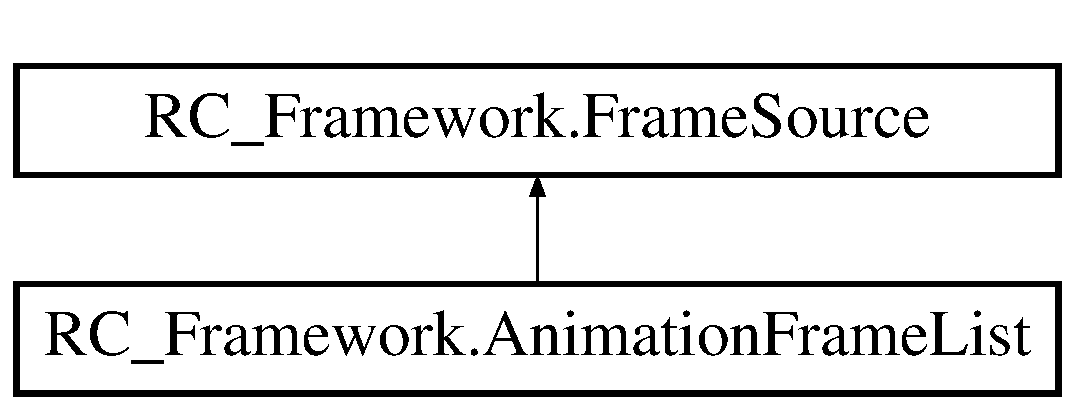
\includegraphics[height=2.000000cm]{class_r_c___framework_1_1_animation_frame_list}
\end{center}
\end{figure}
\subsection*{Public Member Functions}
\begin{DoxyCompactItemize}
\item 
\mbox{\hyperlink{class_r_c___framework_1_1_animation_frame_list_ad4853f5ccf776a762d4a3ca431cf623f}{Animation\+Frame\+List}} (\mbox{\hyperlink{class_r_c___framework_1_1_frame_list}{Frame\+List}} frame\+ListZ, \mbox{\hyperlink{class_r_c___framework_1_1_animation_ticker}{Animation\+Ticker}} anim\+TickerZ)
\item 
\mbox{\hyperlink{class_r_c___framework_1_1_animation_frame_list_aa04cc11efd6dbb3cb04b4e67f63fc670}{Animation\+Frame\+List}} (\mbox{\hyperlink{class_r_c___framework_1_1_frame_source}{Frame\+Source}} frame\+Src, \mbox{\hyperlink{class_r_c___framework_1_1_animation_ticker}{Animation\+Ticker}} anim\+TickerZ)
\item 
override \mbox{\hyperlink{class_r_c___framework_1_1_r_c___frame}{R\+C\+\_\+\+Frame}} \mbox{\hyperlink{class_r_c___framework_1_1_animation_frame_list_aa253565464d98bf955c81702fd3d66a4}{get\+Frame}} (int num)
\begin{DoxyCompactList}\small\item\em This one method must be overridden and return a numbered frame for any given number (or null) \end{DoxyCompactList}\item 
override \mbox{\hyperlink{class_r_c___framework_1_1_r_c___frame}{R\+C\+\_\+\+Frame}} \mbox{\hyperlink{class_r_c___framework_1_1_animation_frame_list_a5bc162ddb15e2ef4f98b72be2720a87b}{get\+Frame}} ()
\begin{DoxyCompactList}\small\item\em This method must be overridden and return the current frame (or null) \end{DoxyCompactList}\item 
override void \mbox{\hyperlink{class_r_c___framework_1_1_animation_frame_list_ad6d3b045da01a972a32f48ae7b7c7598}{Update}} (Game\+Time game\+Time)
\begin{DoxyCompactList}\small\item\em Update so the frames can advance if necessary \end{DoxyCompactList}\item 
void \mbox{\hyperlink{class_r_c___framework_1_1_animation_frame_list_af45c9ca8028ef05f2a23def6bf4f5f82}{set\+Running}} (bool runningQ)
\begin{DoxyCompactList}\small\item\em Wrapper for animation ticker running flag \end{DoxyCompactList}\end{DoxyCompactItemize}
\subsection*{Public Attributes}
\begin{DoxyCompactItemize}
\item 
\mbox{\hyperlink{class_r_c___framework_1_1_animation_ticker}{Animation\+Ticker}} \mbox{\hyperlink{class_r_c___framework_1_1_animation_frame_list_a41409ce75f3131d7008e249296cb95a6}{animation\+Ticker}} =null
\begin{DoxyCompactList}\small\item\em A complicated animation class using a timer of class called \mbox{\hyperlink{class_r_c___framework_1_1_animation_ticker}{Animation\+Ticker}} and a list of frames of class called \mbox{\hyperlink{class_r_c___framework_1_1_frame_list}{Frame\+List}} \end{DoxyCompactList}\item 
\mbox{\hyperlink{class_r_c___framework_1_1_frame_source}{Frame\+Source}} \mbox{\hyperlink{class_r_c___framework_1_1_animation_frame_list_a3dd60d9e75ce6498504a04894f8626bc}{frame\+Source}} =null
\end{DoxyCompactItemize}
\subsection*{Protected Attributes}
\begin{DoxyCompactItemize}
\item 
\mbox{\hyperlink{class_r_c___framework_1_1_frame_list}{Frame\+List}} \mbox{\hyperlink{class_r_c___framework_1_1_animation_frame_list_a138734a263190761b0da537fb830f2a9}{frame\+List}} =null
\end{DoxyCompactItemize}


\subsection{Constructor \& Destructor Documentation}
\mbox{\Hypertarget{class_r_c___framework_1_1_animation_frame_list_ad4853f5ccf776a762d4a3ca431cf623f}\label{class_r_c___framework_1_1_animation_frame_list_ad4853f5ccf776a762d4a3ca431cf623f}} 
\index{R\+C\+\_\+\+Framework\+::\+Animation\+Frame\+List@{R\+C\+\_\+\+Framework\+::\+Animation\+Frame\+List}!Animation\+Frame\+List@{Animation\+Frame\+List}}
\index{Animation\+Frame\+List@{Animation\+Frame\+List}!R\+C\+\_\+\+Framework\+::\+Animation\+Frame\+List@{R\+C\+\_\+\+Framework\+::\+Animation\+Frame\+List}}
\subsubsection{\texorpdfstring{Animation\+Frame\+List()}{AnimationFrameList()}\hspace{0.1cm}{\footnotesize\ttfamily [1/2]}}
{\footnotesize\ttfamily R\+C\+\_\+\+Framework.\+Animation\+Frame\+List.\+Animation\+Frame\+List (\begin{DoxyParamCaption}\item[{\mbox{\hyperlink{class_r_c___framework_1_1_frame_list}{Frame\+List}}}]{frame\+ListZ,  }\item[{\mbox{\hyperlink{class_r_c___framework_1_1_animation_ticker}{Animation\+Ticker}}}]{anim\+TickerZ }\end{DoxyParamCaption})}

\mbox{\Hypertarget{class_r_c___framework_1_1_animation_frame_list_aa04cc11efd6dbb3cb04b4e67f63fc670}\label{class_r_c___framework_1_1_animation_frame_list_aa04cc11efd6dbb3cb04b4e67f63fc670}} 
\index{R\+C\+\_\+\+Framework\+::\+Animation\+Frame\+List@{R\+C\+\_\+\+Framework\+::\+Animation\+Frame\+List}!Animation\+Frame\+List@{Animation\+Frame\+List}}
\index{Animation\+Frame\+List@{Animation\+Frame\+List}!R\+C\+\_\+\+Framework\+::\+Animation\+Frame\+List@{R\+C\+\_\+\+Framework\+::\+Animation\+Frame\+List}}
\subsubsection{\texorpdfstring{Animation\+Frame\+List()}{AnimationFrameList()}\hspace{0.1cm}{\footnotesize\ttfamily [2/2]}}
{\footnotesize\ttfamily R\+C\+\_\+\+Framework.\+Animation\+Frame\+List.\+Animation\+Frame\+List (\begin{DoxyParamCaption}\item[{\mbox{\hyperlink{class_r_c___framework_1_1_frame_source}{Frame\+Source}}}]{frame\+Src,  }\item[{\mbox{\hyperlink{class_r_c___framework_1_1_animation_ticker}{Animation\+Ticker}}}]{anim\+TickerZ }\end{DoxyParamCaption})}



\subsection{Member Function Documentation}
\mbox{\Hypertarget{class_r_c___framework_1_1_animation_frame_list_aa253565464d98bf955c81702fd3d66a4}\label{class_r_c___framework_1_1_animation_frame_list_aa253565464d98bf955c81702fd3d66a4}} 
\index{R\+C\+\_\+\+Framework\+::\+Animation\+Frame\+List@{R\+C\+\_\+\+Framework\+::\+Animation\+Frame\+List}!get\+Frame@{get\+Frame}}
\index{get\+Frame@{get\+Frame}!R\+C\+\_\+\+Framework\+::\+Animation\+Frame\+List@{R\+C\+\_\+\+Framework\+::\+Animation\+Frame\+List}}
\subsubsection{\texorpdfstring{get\+Frame()}{getFrame()}\hspace{0.1cm}{\footnotesize\ttfamily [1/2]}}
{\footnotesize\ttfamily override \mbox{\hyperlink{class_r_c___framework_1_1_r_c___frame}{R\+C\+\_\+\+Frame}} R\+C\+\_\+\+Framework.\+Animation\+Frame\+List.\+get\+Frame (\begin{DoxyParamCaption}\item[{int}]{num }\end{DoxyParamCaption})\hspace{0.3cm}{\ttfamily [virtual]}}



This one method must be overridden and return a numbered frame for any given number (or null) 


\begin{DoxyParams}{Parameters}
{\em num} & \\
\hline
\end{DoxyParams}
\begin{DoxyReturn}{Returns}

\end{DoxyReturn}


Implements \mbox{\hyperlink{class_r_c___framework_1_1_frame_source_a562dc295b5c265ec760227978802eb3a}{R\+C\+\_\+\+Framework.\+Frame\+Source}}.

\mbox{\Hypertarget{class_r_c___framework_1_1_animation_frame_list_a5bc162ddb15e2ef4f98b72be2720a87b}\label{class_r_c___framework_1_1_animation_frame_list_a5bc162ddb15e2ef4f98b72be2720a87b}} 
\index{R\+C\+\_\+\+Framework\+::\+Animation\+Frame\+List@{R\+C\+\_\+\+Framework\+::\+Animation\+Frame\+List}!get\+Frame@{get\+Frame}}
\index{get\+Frame@{get\+Frame}!R\+C\+\_\+\+Framework\+::\+Animation\+Frame\+List@{R\+C\+\_\+\+Framework\+::\+Animation\+Frame\+List}}
\subsubsection{\texorpdfstring{get\+Frame()}{getFrame()}\hspace{0.1cm}{\footnotesize\ttfamily [2/2]}}
{\footnotesize\ttfamily override \mbox{\hyperlink{class_r_c___framework_1_1_r_c___frame}{R\+C\+\_\+\+Frame}} R\+C\+\_\+\+Framework.\+Animation\+Frame\+List.\+get\+Frame (\begin{DoxyParamCaption}{ }\end{DoxyParamCaption})\hspace{0.3cm}{\ttfamily [virtual]}}



This method must be overridden and return the current frame (or null) 


\begin{DoxyParams}{Parameters}
{\em num} & \\
\hline
\end{DoxyParams}
\begin{DoxyReturn}{Returns}

\end{DoxyReturn}


Implements \mbox{\hyperlink{class_r_c___framework_1_1_frame_source_a6fd84a8d608da7d9ff2ff5ab10ed4243}{R\+C\+\_\+\+Framework.\+Frame\+Source}}.

\mbox{\Hypertarget{class_r_c___framework_1_1_animation_frame_list_af45c9ca8028ef05f2a23def6bf4f5f82}\label{class_r_c___framework_1_1_animation_frame_list_af45c9ca8028ef05f2a23def6bf4f5f82}} 
\index{R\+C\+\_\+\+Framework\+::\+Animation\+Frame\+List@{R\+C\+\_\+\+Framework\+::\+Animation\+Frame\+List}!set\+Running@{set\+Running}}
\index{set\+Running@{set\+Running}!R\+C\+\_\+\+Framework\+::\+Animation\+Frame\+List@{R\+C\+\_\+\+Framework\+::\+Animation\+Frame\+List}}
\subsubsection{\texorpdfstring{set\+Running()}{setRunning()}}
{\footnotesize\ttfamily void R\+C\+\_\+\+Framework.\+Animation\+Frame\+List.\+set\+Running (\begin{DoxyParamCaption}\item[{bool}]{runningQ }\end{DoxyParamCaption})}



Wrapper for animation ticker running flag 


\begin{DoxyParams}{Parameters}
{\em runningQ} & \\
\hline
\end{DoxyParams}
\mbox{\Hypertarget{class_r_c___framework_1_1_animation_frame_list_ad6d3b045da01a972a32f48ae7b7c7598}\label{class_r_c___framework_1_1_animation_frame_list_ad6d3b045da01a972a32f48ae7b7c7598}} 
\index{R\+C\+\_\+\+Framework\+::\+Animation\+Frame\+List@{R\+C\+\_\+\+Framework\+::\+Animation\+Frame\+List}!Update@{Update}}
\index{Update@{Update}!R\+C\+\_\+\+Framework\+::\+Animation\+Frame\+List@{R\+C\+\_\+\+Framework\+::\+Animation\+Frame\+List}}
\subsubsection{\texorpdfstring{Update()}{Update()}}
{\footnotesize\ttfamily override void R\+C\+\_\+\+Framework.\+Animation\+Frame\+List.\+Update (\begin{DoxyParamCaption}\item[{Game\+Time}]{game\+Time }\end{DoxyParamCaption})\hspace{0.3cm}{\ttfamily [virtual]}}



Update so the frames can advance if necessary 


\begin{DoxyParams}{Parameters}
{\em game\+Time} & \\
\hline
\end{DoxyParams}


Reimplemented from \mbox{\hyperlink{class_r_c___framework_1_1_frame_source_a4ab94513c0555c16316b540aed1e9144}{R\+C\+\_\+\+Framework.\+Frame\+Source}}.



\subsection{Member Data Documentation}
\mbox{\Hypertarget{class_r_c___framework_1_1_animation_frame_list_a41409ce75f3131d7008e249296cb95a6}\label{class_r_c___framework_1_1_animation_frame_list_a41409ce75f3131d7008e249296cb95a6}} 
\index{R\+C\+\_\+\+Framework\+::\+Animation\+Frame\+List@{R\+C\+\_\+\+Framework\+::\+Animation\+Frame\+List}!animation\+Ticker@{animation\+Ticker}}
\index{animation\+Ticker@{animation\+Ticker}!R\+C\+\_\+\+Framework\+::\+Animation\+Frame\+List@{R\+C\+\_\+\+Framework\+::\+Animation\+Frame\+List}}
\subsubsection{\texorpdfstring{animation\+Ticker}{animationTicker}}
{\footnotesize\ttfamily \mbox{\hyperlink{class_r_c___framework_1_1_animation_ticker}{Animation\+Ticker}} R\+C\+\_\+\+Framework.\+Animation\+Frame\+List.\+animation\+Ticker =null}



A complicated animation class using a timer of class called \mbox{\hyperlink{class_r_c___framework_1_1_animation_ticker}{Animation\+Ticker}} and a list of frames of class called \mbox{\hyperlink{class_r_c___framework_1_1_frame_list}{Frame\+List}} 

To use this class its normal to call it as follows\+:

// first here set up the frame list .... fr\+List \mbox{\hyperlink{class_r_c___framework_1_1_frame_list}{Frame\+List}} = new Frame\+List(); fr\+List.\+add(tex, new Rectangle(0,0,100,100); fr\+List.\+add(tex, new Rectangle(0,0,200,100); fr\+List.\+add(tex2, new Rectangle(0,0,100,100);

// now set up the animation ticker int aseq\mbox{[}\mbox{]} = new aseq\mbox{[}3\mbox{]}; \mbox{\hyperlink{class_r_c___framework_1_1_animation_ticker}{Animation\+Ticker}} an\+Ticker = new Animation\+Ticker(a\+Seq, 0, 3, 9, 0);

// now combine them to what you want \mbox{\hyperlink{class_r_c___framework_1_1_animation_frame_list}{Animation\+Frame\+List}} afl = new Animation\+Frame\+List(fr\+List, an\+Ticker); afl.\+animation\+Ticker.\+animation\+Start();

// finally put them in the sprite or renderable sprite.\+frame\+Source = afl;

// finally start the animation using the animation ticker afl.\+animation\+Ticker.\+animation\+Start();\mbox{\Hypertarget{class_r_c___framework_1_1_animation_frame_list_a138734a263190761b0da537fb830f2a9}\label{class_r_c___framework_1_1_animation_frame_list_a138734a263190761b0da537fb830f2a9}} 
\index{R\+C\+\_\+\+Framework\+::\+Animation\+Frame\+List@{R\+C\+\_\+\+Framework\+::\+Animation\+Frame\+List}!frame\+List@{frame\+List}}
\index{frame\+List@{frame\+List}!R\+C\+\_\+\+Framework\+::\+Animation\+Frame\+List@{R\+C\+\_\+\+Framework\+::\+Animation\+Frame\+List}}
\subsubsection{\texorpdfstring{frame\+List}{frameList}}
{\footnotesize\ttfamily \mbox{\hyperlink{class_r_c___framework_1_1_frame_list}{Frame\+List}} R\+C\+\_\+\+Framework.\+Animation\+Frame\+List.\+frame\+List =null\hspace{0.3cm}{\ttfamily [protected]}}

\mbox{\Hypertarget{class_r_c___framework_1_1_animation_frame_list_a3dd60d9e75ce6498504a04894f8626bc}\label{class_r_c___framework_1_1_animation_frame_list_a3dd60d9e75ce6498504a04894f8626bc}} 
\index{R\+C\+\_\+\+Framework\+::\+Animation\+Frame\+List@{R\+C\+\_\+\+Framework\+::\+Animation\+Frame\+List}!frame\+Source@{frame\+Source}}
\index{frame\+Source@{frame\+Source}!R\+C\+\_\+\+Framework\+::\+Animation\+Frame\+List@{R\+C\+\_\+\+Framework\+::\+Animation\+Frame\+List}}
\subsubsection{\texorpdfstring{frame\+Source}{frameSource}}
{\footnotesize\ttfamily \mbox{\hyperlink{class_r_c___framework_1_1_frame_source}{Frame\+Source}} R\+C\+\_\+\+Framework.\+Animation\+Frame\+List.\+frame\+Source =null}



The documentation for this class was generated from the following file\+:\begin{DoxyCompactItemize}
\item 
F\+:/\+B/\+R\+C\+\_\+\+Framework2018/\+Source/\mbox{\hyperlink{_r_c___frame_8cs}{R\+C\+\_\+\+Frame.\+cs}}\end{DoxyCompactItemize}

\hypertarget{class_r_c___framework_1_1_animation_ticker}{}\section{R\+C\+\_\+\+Framework.\+Animation\+Ticker Class Reference}
\label{class_r_c___framework_1_1_animation_ticker}\index{R\+C\+\_\+\+Framework.\+Animation\+Ticker@{R\+C\+\_\+\+Framework.\+Animation\+Ticker}}


This class just manages a counter to tell the current frame number  


\subsection*{Public Member Functions}
\begin{DoxyCompactItemize}
\item 
\mbox{\hyperlink{class_r_c___framework_1_1_animation_ticker_afb68bed1e4614d31fea99971448af72b}{Animation\+Ticker}} (int\mbox{[}$\,$\mbox{]} anim\+Seq, int first\+FrameZ, int last\+FrameZ, int ticks\+Between\+FramesZ, int anim\+FinishedZ)
\begin{DoxyCompactList}\small\item\em create an animation ticker \end{DoxyCompactList}\item 
void \mbox{\hyperlink{class_r_c___framework_1_1_animation_ticker_a7dc8c7e1833acf289c4ae2d8ef7186c0}{reset\+Animation\+Ticker}} (int\mbox{[}$\,$\mbox{]} anim\+Seq, int first\+FrameZ, int last\+FrameZ, int ticks\+Between\+FramesZ, int anim\+FinishedZ)
\item 
void \mbox{\hyperlink{class_r_c___framework_1_1_animation_ticker_aa01c754af9f362a118156f5114ee8843}{animation\+Start}} ()
\begin{DoxyCompactList}\small\item\em Set the start parameters for the animation sequence \end{DoxyCompactList}\item 
void \mbox{\hyperlink{class_r_c___framework_1_1_animation_ticker_a745c0ec1e44580c17ce60646ba0a8c10}{set\+Anim\+Finished}} (int what\+To\+Do)
\begin{DoxyCompactList}\small\item\em A flag telling what to do when the animation finishes 0 = loop 1 = set first frame 2 = set last frame 3 = set frame = 0 \end{DoxyCompactList}\item 
int \mbox{\hyperlink{class_r_c___framework_1_1_animation_ticker_a5f122a2978abcd1ae930d22fbbf6e07e}{get\+Frame\+Num}} ()
\begin{DoxyCompactList}\small\item\em gets the current frame number -\/ if update is called then all should be good \end{DoxyCompactList}\item 
void \mbox{\hyperlink{class_r_c___framework_1_1_animation_ticker_ad5efbd9a22b71acdb310cbf36bfc3ed4}{pause\+Animation}} (bool state)
\begin{DoxyCompactList}\small\item\em can be used to temporarily pause an animation \end{DoxyCompactList}\item 
void \mbox{\hyperlink{class_r_c___framework_1_1_animation_ticker_a651ebc93d3b81476de57192aa0ed7ac0}{set\+Frame\+Index}} (int frame\+IndexZ)
\begin{DoxyCompactList}\small\item\em generally you wont need this but in theory it can reset an animation to a new point \end{DoxyCompactList}\item 
void \mbox{\hyperlink{class_r_c___framework_1_1_animation_ticker_ab35ac03afdb37b3f59a15eb08c7daa0f}{set\+Frame}} (int frameZ)
\begin{DoxyCompactList}\small\item\em generally you wont need this and you will need to set running to false for it to stop animation \end{DoxyCompactList}\item 
void \mbox{\hyperlink{class_r_c___framework_1_1_animation_ticker_a6d859fd88b02f11b5ce36d72f307f2da}{Update}} (Game\+Time game\+Time)
\begin{DoxyCompactList}\small\item\em Update the animation sequence This routine is usually run in the update routine this routine has game\+Time as a parameter \end{DoxyCompactList}\end{DoxyCompactItemize}
\subsection*{Public Attributes}
\begin{DoxyCompactItemize}
\item 
bool \mbox{\hyperlink{class_r_c___framework_1_1_animation_ticker_aa510bfceffc13acf2a6175094794d783}{running}} = false
\begin{DoxyCompactList}\small\item\em make it tick or not \end{DoxyCompactList}\end{DoxyCompactItemize}


\subsection{Detailed Description}
This class just manages a counter to tell the current frame number 



\subsection{Constructor \& Destructor Documentation}
\mbox{\Hypertarget{class_r_c___framework_1_1_animation_ticker_afb68bed1e4614d31fea99971448af72b}\label{class_r_c___framework_1_1_animation_ticker_afb68bed1e4614d31fea99971448af72b}} 
\index{R\+C\+\_\+\+Framework\+::\+Animation\+Ticker@{R\+C\+\_\+\+Framework\+::\+Animation\+Ticker}!Animation\+Ticker@{Animation\+Ticker}}
\index{Animation\+Ticker@{Animation\+Ticker}!R\+C\+\_\+\+Framework\+::\+Animation\+Ticker@{R\+C\+\_\+\+Framework\+::\+Animation\+Ticker}}
\subsubsection{\texorpdfstring{Animation\+Ticker()}{AnimationTicker()}}
{\footnotesize\ttfamily R\+C\+\_\+\+Framework.\+Animation\+Ticker.\+Animation\+Ticker (\begin{DoxyParamCaption}\item[{int \mbox{[}$\,$\mbox{]}}]{anim\+Seq,  }\item[{int}]{first\+FrameZ,  }\item[{int}]{last\+FrameZ,  }\item[{int}]{ticks\+Between\+FramesZ,  }\item[{int}]{anim\+FinishedZ }\end{DoxyParamCaption})}



create an animation ticker 


\begin{DoxyParams}{Parameters}
{\em anim\+Seq} & \\
\hline
{\em first\+FrameZ} & \\
\hline
{\em last\+FrameZ} & \\
\hline
{\em ticks\+Between\+FramesZ} & \\
\hline
{\em anim\+FinishedZ} & 0=loop, 1=firstframe, 2=lastframe, 3=frame0\\
\hline
\end{DoxyParams}


\subsection{Member Function Documentation}
\mbox{\Hypertarget{class_r_c___framework_1_1_animation_ticker_aa01c754af9f362a118156f5114ee8843}\label{class_r_c___framework_1_1_animation_ticker_aa01c754af9f362a118156f5114ee8843}} 
\index{R\+C\+\_\+\+Framework\+::\+Animation\+Ticker@{R\+C\+\_\+\+Framework\+::\+Animation\+Ticker}!animation\+Start@{animation\+Start}}
\index{animation\+Start@{animation\+Start}!R\+C\+\_\+\+Framework\+::\+Animation\+Ticker@{R\+C\+\_\+\+Framework\+::\+Animation\+Ticker}}
\subsubsection{\texorpdfstring{animation\+Start()}{animationStart()}}
{\footnotesize\ttfamily void R\+C\+\_\+\+Framework.\+Animation\+Ticker.\+animation\+Start (\begin{DoxyParamCaption}{ }\end{DoxyParamCaption})}



Set the start parameters for the animation sequence 

\mbox{\Hypertarget{class_r_c___framework_1_1_animation_ticker_a5f122a2978abcd1ae930d22fbbf6e07e}\label{class_r_c___framework_1_1_animation_ticker_a5f122a2978abcd1ae930d22fbbf6e07e}} 
\index{R\+C\+\_\+\+Framework\+::\+Animation\+Ticker@{R\+C\+\_\+\+Framework\+::\+Animation\+Ticker}!get\+Frame\+Num@{get\+Frame\+Num}}
\index{get\+Frame\+Num@{get\+Frame\+Num}!R\+C\+\_\+\+Framework\+::\+Animation\+Ticker@{R\+C\+\_\+\+Framework\+::\+Animation\+Ticker}}
\subsubsection{\texorpdfstring{get\+Frame\+Num()}{getFrameNum()}}
{\footnotesize\ttfamily int R\+C\+\_\+\+Framework.\+Animation\+Ticker.\+get\+Frame\+Num (\begin{DoxyParamCaption}{ }\end{DoxyParamCaption})}



gets the current frame number -\/ if update is called then all should be good 

\begin{DoxyReturn}{Returns}

\end{DoxyReturn}
\mbox{\Hypertarget{class_r_c___framework_1_1_animation_ticker_ad5efbd9a22b71acdb310cbf36bfc3ed4}\label{class_r_c___framework_1_1_animation_ticker_ad5efbd9a22b71acdb310cbf36bfc3ed4}} 
\index{R\+C\+\_\+\+Framework\+::\+Animation\+Ticker@{R\+C\+\_\+\+Framework\+::\+Animation\+Ticker}!pause\+Animation@{pause\+Animation}}
\index{pause\+Animation@{pause\+Animation}!R\+C\+\_\+\+Framework\+::\+Animation\+Ticker@{R\+C\+\_\+\+Framework\+::\+Animation\+Ticker}}
\subsubsection{\texorpdfstring{pause\+Animation()}{pauseAnimation()}}
{\footnotesize\ttfamily void R\+C\+\_\+\+Framework.\+Animation\+Ticker.\+pause\+Animation (\begin{DoxyParamCaption}\item[{bool}]{state }\end{DoxyParamCaption})}



can be used to temporarily pause an animation 


\begin{DoxyParams}{Parameters}
{\em state} & \\
\hline
\end{DoxyParams}
\mbox{\Hypertarget{class_r_c___framework_1_1_animation_ticker_a7dc8c7e1833acf289c4ae2d8ef7186c0}\label{class_r_c___framework_1_1_animation_ticker_a7dc8c7e1833acf289c4ae2d8ef7186c0}} 
\index{R\+C\+\_\+\+Framework\+::\+Animation\+Ticker@{R\+C\+\_\+\+Framework\+::\+Animation\+Ticker}!reset\+Animation\+Ticker@{reset\+Animation\+Ticker}}
\index{reset\+Animation\+Ticker@{reset\+Animation\+Ticker}!R\+C\+\_\+\+Framework\+::\+Animation\+Ticker@{R\+C\+\_\+\+Framework\+::\+Animation\+Ticker}}
\subsubsection{\texorpdfstring{reset\+Animation\+Ticker()}{resetAnimationTicker()}}
{\footnotesize\ttfamily void R\+C\+\_\+\+Framework.\+Animation\+Ticker.\+reset\+Animation\+Ticker (\begin{DoxyParamCaption}\item[{int \mbox{[}$\,$\mbox{]}}]{anim\+Seq,  }\item[{int}]{first\+FrameZ,  }\item[{int}]{last\+FrameZ,  }\item[{int}]{ticks\+Between\+FramesZ,  }\item[{int}]{anim\+FinishedZ }\end{DoxyParamCaption})}

\mbox{\Hypertarget{class_r_c___framework_1_1_animation_ticker_a745c0ec1e44580c17ce60646ba0a8c10}\label{class_r_c___framework_1_1_animation_ticker_a745c0ec1e44580c17ce60646ba0a8c10}} 
\index{R\+C\+\_\+\+Framework\+::\+Animation\+Ticker@{R\+C\+\_\+\+Framework\+::\+Animation\+Ticker}!set\+Anim\+Finished@{set\+Anim\+Finished}}
\index{set\+Anim\+Finished@{set\+Anim\+Finished}!R\+C\+\_\+\+Framework\+::\+Animation\+Ticker@{R\+C\+\_\+\+Framework\+::\+Animation\+Ticker}}
\subsubsection{\texorpdfstring{set\+Anim\+Finished()}{setAnimFinished()}}
{\footnotesize\ttfamily void R\+C\+\_\+\+Framework.\+Animation\+Ticker.\+set\+Anim\+Finished (\begin{DoxyParamCaption}\item[{int}]{what\+To\+Do }\end{DoxyParamCaption})}



A flag telling what to do when the animation finishes 0 = loop 1 = set first frame 2 = set last frame 3 = set frame = 0 


\begin{DoxyParams}{Parameters}
{\em what\+To\+Do} & \\
\hline
\end{DoxyParams}
\mbox{\Hypertarget{class_r_c___framework_1_1_animation_ticker_ab35ac03afdb37b3f59a15eb08c7daa0f}\label{class_r_c___framework_1_1_animation_ticker_ab35ac03afdb37b3f59a15eb08c7daa0f}} 
\index{R\+C\+\_\+\+Framework\+::\+Animation\+Ticker@{R\+C\+\_\+\+Framework\+::\+Animation\+Ticker}!set\+Frame@{set\+Frame}}
\index{set\+Frame@{set\+Frame}!R\+C\+\_\+\+Framework\+::\+Animation\+Ticker@{R\+C\+\_\+\+Framework\+::\+Animation\+Ticker}}
\subsubsection{\texorpdfstring{set\+Frame()}{setFrame()}}
{\footnotesize\ttfamily void R\+C\+\_\+\+Framework.\+Animation\+Ticker.\+set\+Frame (\begin{DoxyParamCaption}\item[{int}]{frameZ }\end{DoxyParamCaption})}



generally you wont need this and you will need to set running to false for it to stop animation 


\begin{DoxyParams}{Parameters}
{\em frameZ} & \\
\hline
\end{DoxyParams}
\mbox{\Hypertarget{class_r_c___framework_1_1_animation_ticker_a651ebc93d3b81476de57192aa0ed7ac0}\label{class_r_c___framework_1_1_animation_ticker_a651ebc93d3b81476de57192aa0ed7ac0}} 
\index{R\+C\+\_\+\+Framework\+::\+Animation\+Ticker@{R\+C\+\_\+\+Framework\+::\+Animation\+Ticker}!set\+Frame\+Index@{set\+Frame\+Index}}
\index{set\+Frame\+Index@{set\+Frame\+Index}!R\+C\+\_\+\+Framework\+::\+Animation\+Ticker@{R\+C\+\_\+\+Framework\+::\+Animation\+Ticker}}
\subsubsection{\texorpdfstring{set\+Frame\+Index()}{setFrameIndex()}}
{\footnotesize\ttfamily void R\+C\+\_\+\+Framework.\+Animation\+Ticker.\+set\+Frame\+Index (\begin{DoxyParamCaption}\item[{int}]{frame\+IndexZ }\end{DoxyParamCaption})}



generally you wont need this but in theory it can reset an animation to a new point 


\begin{DoxyParams}{Parameters}
{\em frameZ} & \\
\hline
\end{DoxyParams}
\mbox{\Hypertarget{class_r_c___framework_1_1_animation_ticker_a6d859fd88b02f11b5ce36d72f307f2da}\label{class_r_c___framework_1_1_animation_ticker_a6d859fd88b02f11b5ce36d72f307f2da}} 
\index{R\+C\+\_\+\+Framework\+::\+Animation\+Ticker@{R\+C\+\_\+\+Framework\+::\+Animation\+Ticker}!Update@{Update}}
\index{Update@{Update}!R\+C\+\_\+\+Framework\+::\+Animation\+Ticker@{R\+C\+\_\+\+Framework\+::\+Animation\+Ticker}}
\subsubsection{\texorpdfstring{Update()}{Update()}}
{\footnotesize\ttfamily void R\+C\+\_\+\+Framework.\+Animation\+Ticker.\+Update (\begin{DoxyParamCaption}\item[{Game\+Time}]{game\+Time }\end{DoxyParamCaption})}



Update the animation sequence This routine is usually run in the update routine this routine has game\+Time as a parameter 



\subsection{Member Data Documentation}
\mbox{\Hypertarget{class_r_c___framework_1_1_animation_ticker_aa510bfceffc13acf2a6175094794d783}\label{class_r_c___framework_1_1_animation_ticker_aa510bfceffc13acf2a6175094794d783}} 
\index{R\+C\+\_\+\+Framework\+::\+Animation\+Ticker@{R\+C\+\_\+\+Framework\+::\+Animation\+Ticker}!running@{running}}
\index{running@{running}!R\+C\+\_\+\+Framework\+::\+Animation\+Ticker@{R\+C\+\_\+\+Framework\+::\+Animation\+Ticker}}
\subsubsection{\texorpdfstring{running}{running}}
{\footnotesize\ttfamily bool R\+C\+\_\+\+Framework.\+Animation\+Ticker.\+running = false}



make it tick or not 



The documentation for this class was generated from the following file\+:\begin{DoxyCompactItemize}
\item 
F\+:/\+B/\+R\+C\+\_\+\+Framework2018/\+Source/\mbox{\hyperlink{_r_c___frame_8cs}{R\+C\+\_\+\+Frame.\+cs}}\end{DoxyCompactItemize}

\hypertarget{class_r_c___framework_1_1_attached_text}{}\section{R\+C\+\_\+\+Framework.\+Attached\+Text Class Reference}
\label{class_r_c___framework_1_1_attached_text}\index{R\+C\+\_\+\+Framework.\+Attached\+Text@{R\+C\+\_\+\+Framework.\+Attached\+Text}}


this class simply attaches a lump of text to the sprite it can have its own text or use the text property of sprite useing the text property of sprite is recomended  


Inheritance diagram for R\+C\+\_\+\+Framework.\+Attached\+Text\+:\begin{figure}[H]
\begin{center}
\leavevmode
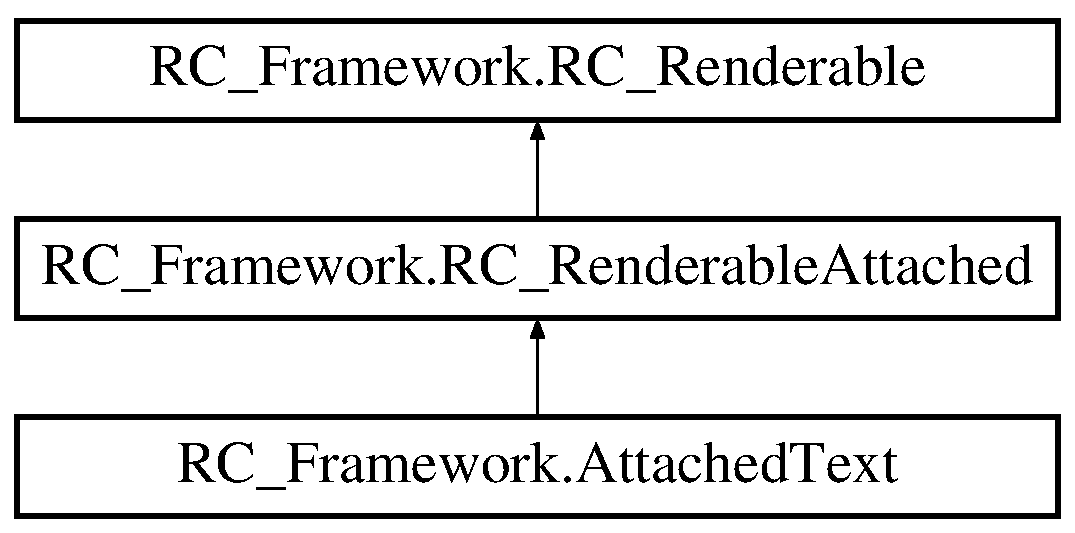
\includegraphics[height=3.000000cm]{class_r_c___framework_1_1_attached_text}
\end{center}
\end{figure}
\subsection*{Public Member Functions}
\begin{DoxyCompactItemize}
\item 
\mbox{\hyperlink{class_r_c___framework_1_1_attached_text_a39ea4d4bc1ab6294a506e02826dc8a19}{Attached\+Text}} (Color colorZ, Sprite\+Font fontZ, Vector2 offsetZ, string textZ)
\item 
\mbox{\hyperlink{class_r_c___framework_1_1_attached_text_a24a5fb5d3b20c5e50ce4d077f0921554}{Attached\+Text}} (Color colorZ, Sprite\+Font fontZ, Vector2 offsetZ)
\item 
\mbox{\hyperlink{class_r_c___framework_1_1_attached_text_a457b1f3860d89be63a912e22e254041b}{Attached\+Text}} (Color colorZ, Sprite\+Font fontZ)
\item 
override void \mbox{\hyperlink{class_r_c___framework_1_1_attached_text_a5972b29f469c9c005a46652ab448411c}{Draw}} (Sprite\+Batch sb)
\begin{DoxyCompactList}\small\item\em Standard draw routine which assumes the renderable knows where it is \end{DoxyCompactList}\end{DoxyCompactItemize}
\subsection*{Public Attributes}
\begin{DoxyCompactItemize}
\item 
Vector2 \mbox{\hyperlink{class_r_c___framework_1_1_attached_text_a7305fc71a2f3bcba1e64dfd179dbb847}{offset}} = new Vector2(0, -\/1)
\item 
Sprite\+Font \mbox{\hyperlink{class_r_c___framework_1_1_attached_text_a890a2a05d38c24d664cdfa28e96b6092}{font}}
\end{DoxyCompactItemize}
\subsection*{Additional Inherited Members}


\subsection{Detailed Description}
this class simply attaches a lump of text to the sprite it can have its own text or use the text property of sprite useing the text property of sprite is recomended 



\subsection{Constructor \& Destructor Documentation}
\mbox{\Hypertarget{class_r_c___framework_1_1_attached_text_a39ea4d4bc1ab6294a506e02826dc8a19}\label{class_r_c___framework_1_1_attached_text_a39ea4d4bc1ab6294a506e02826dc8a19}} 
\index{R\+C\+\_\+\+Framework\+::\+Attached\+Text@{R\+C\+\_\+\+Framework\+::\+Attached\+Text}!Attached\+Text@{Attached\+Text}}
\index{Attached\+Text@{Attached\+Text}!R\+C\+\_\+\+Framework\+::\+Attached\+Text@{R\+C\+\_\+\+Framework\+::\+Attached\+Text}}
\subsubsection{\texorpdfstring{Attached\+Text()}{AttachedText()}\hspace{0.1cm}{\footnotesize\ttfamily [1/3]}}
{\footnotesize\ttfamily R\+C\+\_\+\+Framework.\+Attached\+Text.\+Attached\+Text (\begin{DoxyParamCaption}\item[{Color}]{colorZ,  }\item[{Sprite\+Font}]{fontZ,  }\item[{Vector2}]{offsetZ,  }\item[{string}]{textZ }\end{DoxyParamCaption})}

\mbox{\Hypertarget{class_r_c___framework_1_1_attached_text_a24a5fb5d3b20c5e50ce4d077f0921554}\label{class_r_c___framework_1_1_attached_text_a24a5fb5d3b20c5e50ce4d077f0921554}} 
\index{R\+C\+\_\+\+Framework\+::\+Attached\+Text@{R\+C\+\_\+\+Framework\+::\+Attached\+Text}!Attached\+Text@{Attached\+Text}}
\index{Attached\+Text@{Attached\+Text}!R\+C\+\_\+\+Framework\+::\+Attached\+Text@{R\+C\+\_\+\+Framework\+::\+Attached\+Text}}
\subsubsection{\texorpdfstring{Attached\+Text()}{AttachedText()}\hspace{0.1cm}{\footnotesize\ttfamily [2/3]}}
{\footnotesize\ttfamily R\+C\+\_\+\+Framework.\+Attached\+Text.\+Attached\+Text (\begin{DoxyParamCaption}\item[{Color}]{colorZ,  }\item[{Sprite\+Font}]{fontZ,  }\item[{Vector2}]{offsetZ }\end{DoxyParamCaption})}

\mbox{\Hypertarget{class_r_c___framework_1_1_attached_text_a457b1f3860d89be63a912e22e254041b}\label{class_r_c___framework_1_1_attached_text_a457b1f3860d89be63a912e22e254041b}} 
\index{R\+C\+\_\+\+Framework\+::\+Attached\+Text@{R\+C\+\_\+\+Framework\+::\+Attached\+Text}!Attached\+Text@{Attached\+Text}}
\index{Attached\+Text@{Attached\+Text}!R\+C\+\_\+\+Framework\+::\+Attached\+Text@{R\+C\+\_\+\+Framework\+::\+Attached\+Text}}
\subsubsection{\texorpdfstring{Attached\+Text()}{AttachedText()}\hspace{0.1cm}{\footnotesize\ttfamily [3/3]}}
{\footnotesize\ttfamily R\+C\+\_\+\+Framework.\+Attached\+Text.\+Attached\+Text (\begin{DoxyParamCaption}\item[{Color}]{colorZ,  }\item[{Sprite\+Font}]{fontZ }\end{DoxyParamCaption})}



\subsection{Member Function Documentation}
\mbox{\Hypertarget{class_r_c___framework_1_1_attached_text_a5972b29f469c9c005a46652ab448411c}\label{class_r_c___framework_1_1_attached_text_a5972b29f469c9c005a46652ab448411c}} 
\index{R\+C\+\_\+\+Framework\+::\+Attached\+Text@{R\+C\+\_\+\+Framework\+::\+Attached\+Text}!Draw@{Draw}}
\index{Draw@{Draw}!R\+C\+\_\+\+Framework\+::\+Attached\+Text@{R\+C\+\_\+\+Framework\+::\+Attached\+Text}}
\subsubsection{\texorpdfstring{Draw()}{Draw()}}
{\footnotesize\ttfamily override void R\+C\+\_\+\+Framework.\+Attached\+Text.\+Draw (\begin{DoxyParamCaption}\item[{Sprite\+Batch}]{sb }\end{DoxyParamCaption})\hspace{0.3cm}{\ttfamily [virtual]}}



Standard draw routine which assumes the renderable knows where it is 


\begin{DoxyParams}{Parameters}
{\em sb} & \\
\hline
\end{DoxyParams}


Reimplemented from \mbox{\hyperlink{class_r_c___framework_1_1_r_c___renderable_acc26db34e382a25a989c4c0dd0354b23}{R\+C\+\_\+\+Framework.\+R\+C\+\_\+\+Renderable}}.



\subsection{Member Data Documentation}
\mbox{\Hypertarget{class_r_c___framework_1_1_attached_text_a890a2a05d38c24d664cdfa28e96b6092}\label{class_r_c___framework_1_1_attached_text_a890a2a05d38c24d664cdfa28e96b6092}} 
\index{R\+C\+\_\+\+Framework\+::\+Attached\+Text@{R\+C\+\_\+\+Framework\+::\+Attached\+Text}!font@{font}}
\index{font@{font}!R\+C\+\_\+\+Framework\+::\+Attached\+Text@{R\+C\+\_\+\+Framework\+::\+Attached\+Text}}
\subsubsection{\texorpdfstring{font}{font}}
{\footnotesize\ttfamily Sprite\+Font R\+C\+\_\+\+Framework.\+Attached\+Text.\+font}

\mbox{\Hypertarget{class_r_c___framework_1_1_attached_text_a7305fc71a2f3bcba1e64dfd179dbb847}\label{class_r_c___framework_1_1_attached_text_a7305fc71a2f3bcba1e64dfd179dbb847}} 
\index{R\+C\+\_\+\+Framework\+::\+Attached\+Text@{R\+C\+\_\+\+Framework\+::\+Attached\+Text}!offset@{offset}}
\index{offset@{offset}!R\+C\+\_\+\+Framework\+::\+Attached\+Text@{R\+C\+\_\+\+Framework\+::\+Attached\+Text}}
\subsubsection{\texorpdfstring{offset}{offset}}
{\footnotesize\ttfamily Vector2 R\+C\+\_\+\+Framework.\+Attached\+Text.\+offset = new Vector2(0, -\/1)}



The documentation for this class was generated from the following file\+:\begin{DoxyCompactItemize}
\item 
F\+:/\+B/\+R\+C\+\_\+\+Framework2018/\+Source/\mbox{\hyperlink{_r_c___renderable_attached_8cs}{R\+C\+\_\+\+Renderable\+Attached.\+cs}}\end{DoxyCompactItemize}

\hypertarget{class_r_c___framework_1_1_attached_texture_fade}{}\section{R\+C\+\_\+\+Framework.\+Attached\+Texture\+Fade Class Reference}
\label{class_r_c___framework_1_1_attached_texture_fade}\index{R\+C\+\_\+\+Framework.\+Attached\+Texture\+Fade@{R\+C\+\_\+\+Framework.\+Attached\+Texture\+Fade}}


Fades and resizes a texture At end it can loop , go inactive or reverse its a fairly sophisticated tool usable for a lot of diferent eye candy effects remeber to run update  


Inheritance diagram for R\+C\+\_\+\+Framework.\+Attached\+Texture\+Fade\+:\begin{figure}[H]
\begin{center}
\leavevmode
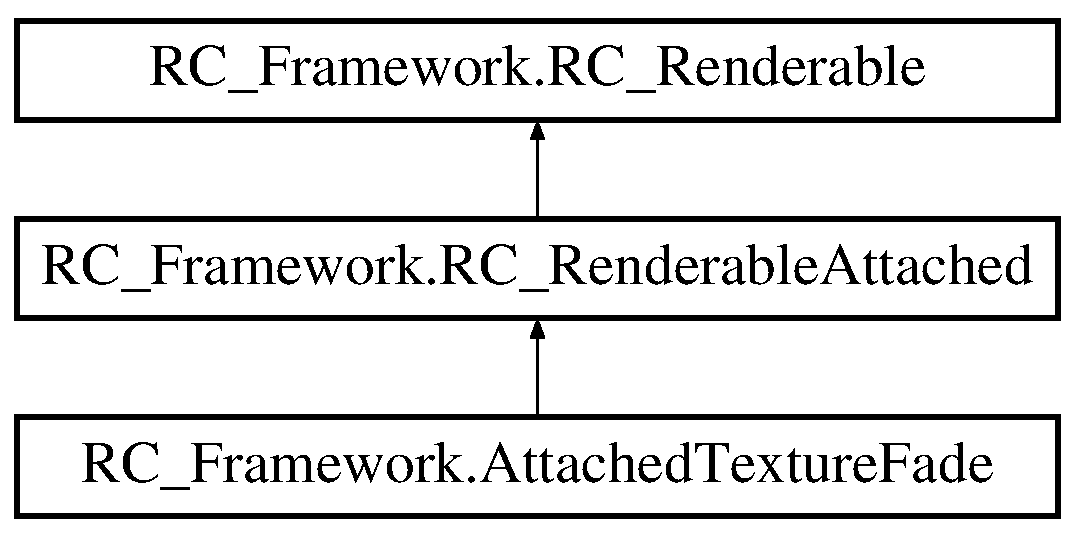
\includegraphics[height=3.000000cm]{class_r_c___framework_1_1_attached_texture_fade}
\end{center}
\end{figure}
\subsection*{Public Member Functions}
\begin{DoxyCompactItemize}
\item 
\mbox{\hyperlink{class_r_c___framework_1_1_attached_texture_fade_a48153baf36d718ea055287af0688a691}{Attached\+Texture\+Fade}} (Texture2D texZ, Rectangle init\+FrameZ, Rectangle final\+FrameZ, Color init\+ColourZ, Color final\+ColourZ, int fade\+TicksZ)
\item 
void \mbox{\hyperlink{class_r_c___framework_1_1_attached_texture_fade_a8b51be50a28199ec67abb43faeedfa73}{setloop}} (int loopQ)
\item 
override void \mbox{\hyperlink{class_r_c___framework_1_1_attached_texture_fade_a93612655099524c9059b6ae9437bda59}{Draw}} (Sprite\+Batch sb)
\begin{DoxyCompactList}\small\item\em Standard draw routine which assumes the renderable knows where it is \end{DoxyCompactList}\item 
override void \mbox{\hyperlink{class_r_c___framework_1_1_attached_texture_fade_a7da61ac25b6b39b6984b5c26547e2291}{Update}} (Game\+Time game\+Time)
\item 
override void \mbox{\hyperlink{class_r_c___framework_1_1_attached_texture_fade_ad5760d7529afe100e6dd7fbe4ecc7b38}{reset}} ()
\end{DoxyCompactItemize}
\subsection*{Public Attributes}
\begin{DoxyCompactItemize}
\item 
int \mbox{\hyperlink{class_r_c___framework_1_1_attached_texture_fade_a4e1a8e468a64463a598f43f3a347e7c4}{loop}}
\end{DoxyCompactItemize}
\subsection*{Properties}
\begin{DoxyCompactItemize}
\item 
Rectangle \mbox{\hyperlink{class_r_c___framework_1_1_attached_texture_fade_a2b22f8a915cad35ae249c3cab1b8272b}{source\+Frame}}\hspace{0.3cm}{\ttfamily  \mbox{[}get, set\mbox{]}}
\end{DoxyCompactItemize}


\subsection{Detailed Description}
Fades and resizes a texture At end it can loop , go inactive or reverse its a fairly sophisticated tool usable for a lot of diferent eye candy effects remeber to run update 



\subsection{Constructor \& Destructor Documentation}
\mbox{\Hypertarget{class_r_c___framework_1_1_attached_texture_fade_a48153baf36d718ea055287af0688a691}\label{class_r_c___framework_1_1_attached_texture_fade_a48153baf36d718ea055287af0688a691}} 
\index{R\+C\+\_\+\+Framework\+::\+Attached\+Texture\+Fade@{R\+C\+\_\+\+Framework\+::\+Attached\+Texture\+Fade}!Attached\+Texture\+Fade@{Attached\+Texture\+Fade}}
\index{Attached\+Texture\+Fade@{Attached\+Texture\+Fade}!R\+C\+\_\+\+Framework\+::\+Attached\+Texture\+Fade@{R\+C\+\_\+\+Framework\+::\+Attached\+Texture\+Fade}}
\subsubsection{\texorpdfstring{Attached\+Texture\+Fade()}{AttachedTextureFade()}}
{\footnotesize\ttfamily R\+C\+\_\+\+Framework.\+Attached\+Texture\+Fade.\+Attached\+Texture\+Fade (\begin{DoxyParamCaption}\item[{Texture2D}]{texZ,  }\item[{Rectangle}]{init\+FrameZ,  }\item[{Rectangle}]{final\+FrameZ,  }\item[{Color}]{init\+ColourZ,  }\item[{Color}]{final\+ColourZ,  }\item[{int}]{fade\+TicksZ }\end{DoxyParamCaption})}



\subsection{Member Function Documentation}
\mbox{\Hypertarget{class_r_c___framework_1_1_attached_texture_fade_a93612655099524c9059b6ae9437bda59}\label{class_r_c___framework_1_1_attached_texture_fade_a93612655099524c9059b6ae9437bda59}} 
\index{R\+C\+\_\+\+Framework\+::\+Attached\+Texture\+Fade@{R\+C\+\_\+\+Framework\+::\+Attached\+Texture\+Fade}!Draw@{Draw}}
\index{Draw@{Draw}!R\+C\+\_\+\+Framework\+::\+Attached\+Texture\+Fade@{R\+C\+\_\+\+Framework\+::\+Attached\+Texture\+Fade}}
\subsubsection{\texorpdfstring{Draw()}{Draw()}}
{\footnotesize\ttfamily override void R\+C\+\_\+\+Framework.\+Attached\+Texture\+Fade.\+Draw (\begin{DoxyParamCaption}\item[{Sprite\+Batch}]{sb }\end{DoxyParamCaption})\hspace{0.3cm}{\ttfamily [virtual]}}



Standard draw routine which assumes the renderable knows where it is 


\begin{DoxyParams}{Parameters}
{\em sb} & \\
\hline
\end{DoxyParams}


Reimplemented from \mbox{\hyperlink{class_r_c___framework_1_1_r_c___renderable_acc26db34e382a25a989c4c0dd0354b23}{R\+C\+\_\+\+Framework.\+R\+C\+\_\+\+Renderable}}.

\mbox{\Hypertarget{class_r_c___framework_1_1_attached_texture_fade_ad5760d7529afe100e6dd7fbe4ecc7b38}\label{class_r_c___framework_1_1_attached_texture_fade_ad5760d7529afe100e6dd7fbe4ecc7b38}} 
\index{R\+C\+\_\+\+Framework\+::\+Attached\+Texture\+Fade@{R\+C\+\_\+\+Framework\+::\+Attached\+Texture\+Fade}!reset@{reset}}
\index{reset@{reset}!R\+C\+\_\+\+Framework\+::\+Attached\+Texture\+Fade@{R\+C\+\_\+\+Framework\+::\+Attached\+Texture\+Fade}}
\subsubsection{\texorpdfstring{reset()}{reset()}}
{\footnotesize\ttfamily override void R\+C\+\_\+\+Framework.\+Attached\+Texture\+Fade.\+reset (\begin{DoxyParamCaption}{ }\end{DoxyParamCaption})\hspace{0.3cm}{\ttfamily [virtual]}}



Reimplemented from \mbox{\hyperlink{class_r_c___framework_1_1_r_c___renderable_ae65ce69704d15963789f421b58618b1f}{R\+C\+\_\+\+Framework.\+R\+C\+\_\+\+Renderable}}.

\mbox{\Hypertarget{class_r_c___framework_1_1_attached_texture_fade_a8b51be50a28199ec67abb43faeedfa73}\label{class_r_c___framework_1_1_attached_texture_fade_a8b51be50a28199ec67abb43faeedfa73}} 
\index{R\+C\+\_\+\+Framework\+::\+Attached\+Texture\+Fade@{R\+C\+\_\+\+Framework\+::\+Attached\+Texture\+Fade}!setloop@{setloop}}
\index{setloop@{setloop}!R\+C\+\_\+\+Framework\+::\+Attached\+Texture\+Fade@{R\+C\+\_\+\+Framework\+::\+Attached\+Texture\+Fade}}
\subsubsection{\texorpdfstring{setloop()}{setloop()}}
{\footnotesize\ttfamily void R\+C\+\_\+\+Framework.\+Attached\+Texture\+Fade.\+setloop (\begin{DoxyParamCaption}\item[{int}]{loopQ }\end{DoxyParamCaption})}

\mbox{\Hypertarget{class_r_c___framework_1_1_attached_texture_fade_a7da61ac25b6b39b6984b5c26547e2291}\label{class_r_c___framework_1_1_attached_texture_fade_a7da61ac25b6b39b6984b5c26547e2291}} 
\index{R\+C\+\_\+\+Framework\+::\+Attached\+Texture\+Fade@{R\+C\+\_\+\+Framework\+::\+Attached\+Texture\+Fade}!Update@{Update}}
\index{Update@{Update}!R\+C\+\_\+\+Framework\+::\+Attached\+Texture\+Fade@{R\+C\+\_\+\+Framework\+::\+Attached\+Texture\+Fade}}
\subsubsection{\texorpdfstring{Update()}{Update()}}
{\footnotesize\ttfamily override void R\+C\+\_\+\+Framework.\+Attached\+Texture\+Fade.\+Update (\begin{DoxyParamCaption}\item[{Game\+Time}]{game\+Time }\end{DoxyParamCaption})\hspace{0.3cm}{\ttfamily [virtual]}}



Reimplemented from \mbox{\hyperlink{class_r_c___framework_1_1_r_c___renderable_a5745bedc7ba0587aa1e1d8563c357228}{R\+C\+\_\+\+Framework.\+R\+C\+\_\+\+Renderable}}.



\subsection{Member Data Documentation}
\mbox{\Hypertarget{class_r_c___framework_1_1_attached_texture_fade_a4e1a8e468a64463a598f43f3a347e7c4}\label{class_r_c___framework_1_1_attached_texture_fade_a4e1a8e468a64463a598f43f3a347e7c4}} 
\index{R\+C\+\_\+\+Framework\+::\+Attached\+Texture\+Fade@{R\+C\+\_\+\+Framework\+::\+Attached\+Texture\+Fade}!loop@{loop}}
\index{loop@{loop}!R\+C\+\_\+\+Framework\+::\+Attached\+Texture\+Fade@{R\+C\+\_\+\+Framework\+::\+Attached\+Texture\+Fade}}
\subsubsection{\texorpdfstring{loop}{loop}}
{\footnotesize\ttfamily int R\+C\+\_\+\+Framework.\+Attached\+Texture\+Fade.\+loop}



\subsection{Property Documentation}
\mbox{\Hypertarget{class_r_c___framework_1_1_attached_texture_fade_a2b22f8a915cad35ae249c3cab1b8272b}\label{class_r_c___framework_1_1_attached_texture_fade_a2b22f8a915cad35ae249c3cab1b8272b}} 
\index{R\+C\+\_\+\+Framework\+::\+Attached\+Texture\+Fade@{R\+C\+\_\+\+Framework\+::\+Attached\+Texture\+Fade}!source\+Frame@{source\+Frame}}
\index{source\+Frame@{source\+Frame}!R\+C\+\_\+\+Framework\+::\+Attached\+Texture\+Fade@{R\+C\+\_\+\+Framework\+::\+Attached\+Texture\+Fade}}
\subsubsection{\texorpdfstring{source\+Frame}{sourceFrame}}
{\footnotesize\ttfamily Rectangle R\+C\+\_\+\+Framework.\+Attached\+Texture\+Fade.\+source\+Frame\hspace{0.3cm}{\ttfamily [get]}, {\ttfamily [set]}}



The documentation for this class was generated from the following file\+:\begin{DoxyCompactItemize}
\item 
F\+:/\+B/\+R\+C\+\_\+\+Framework2018/\+Source/\mbox{\hyperlink{_r_c___renderable_attached_8cs}{R\+C\+\_\+\+Renderable\+Attached.\+cs}}\end{DoxyCompactItemize}

\hypertarget{class_r_c___framework_1_1_blinking_boxes}{}\section{R\+C\+\_\+\+Framework.\+Blinking\+Boxes Class Reference}
\label{class_r_c___framework_1_1_blinking_boxes}\index{R\+C\+\_\+\+Framework.\+Blinking\+Boxes@{R\+C\+\_\+\+Framework.\+Blinking\+Boxes}}


Boxes that blink randomly -\/ for eyecandy on control pannels and computers and things blinktype = 0 for totally random new colour any other is a delta for cycling starttype = 0 for totally random new colour 1 = same colour 2 = cycle colours Example calling sequence is r8a = new \mbox{\hyperlink{class_r_c___framework_1_1_blinking_boxes}{Blinking\+Boxes}}(new Rectangle(10, 10, 200, 100), new Vector2(60, 30), new Vector2(2, 4), 4, 3, 5, 12); r8a.\+set\+Timing(30, 30, 0, 0); r8a.\+add\+Color(Color.\+White); r8a.\+add\+Color(Color.\+Gray); r8a.\+add\+Color(new Color(50,200,7)); r8a.\+add\+Color(Color.\+Red); r8a.\+add\+Color(Color.\+Green);  


Inheritance diagram for R\+C\+\_\+\+Framework.\+Blinking\+Boxes\+:\begin{figure}[H]
\begin{center}
\leavevmode
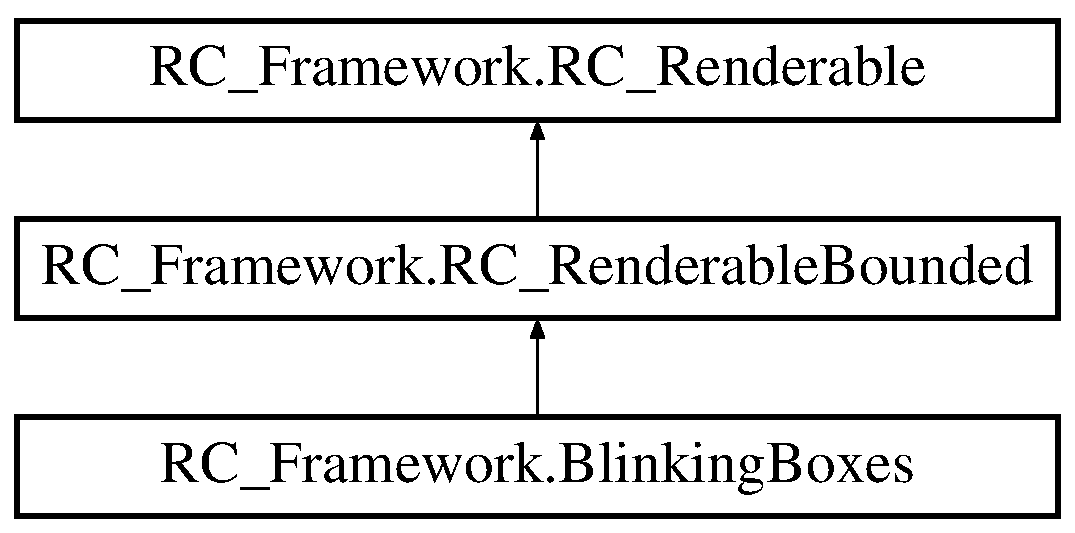
\includegraphics[height=3.000000cm]{class_r_c___framework_1_1_blinking_boxes}
\end{center}
\end{figure}
\subsection*{Public Member Functions}
\begin{DoxyCompactItemize}
\item 
\mbox{\hyperlink{class_r_c___framework_1_1_blinking_boxes_a16ee508e4fa77310bb4305a16a199e95}{Blinking\+Boxes}} (Rectangle \mbox{\hyperlink{class_r_c___framework_1_1_r_c___renderable_bounded_aabcb0f8cd56a2e7b6209f8530194aff1}{boundz}}, Vector2 size\+Of\+Boxx, Vector2 gap\+Between\+Boxez, int num\+Of\+BoxezX, int num\+Of\+BoxezY, int num\+Of\+Colorz, int random\+Seed)
\item 
void \mbox{\hyperlink{class_r_c___framework_1_1_blinking_boxes_a1037bf0c922befbecbdca455d7f6165b}{set\+Stock\+Colours}} ()
\item 
void \mbox{\hyperlink{class_r_c___framework_1_1_blinking_boxes_a2166422cce34c57fb9d77627699c74eb}{set\+Stock\+Colours\+With\+Trans}} ()
\item 
void \mbox{\hyperlink{class_r_c___framework_1_1_blinking_boxes_a6435042084daac78ccd87d801d6a397d}{set\+Stock\+Colours\+With\+Lots\+Trans}} ()
\item 
void \mbox{\hyperlink{class_r_c___framework_1_1_blinking_boxes_ac28bc5c94fe42c132b822745ef292e46}{set\+Timing}} (int update\+ModuloZ, float percent\+Chance\+Of\+ChangeZ, int blink\+TypeZ, int start\+TypeZ)
\item 
void \mbox{\hyperlink{class_r_c___framework_1_1_blinking_boxes_a5e2d89da8ee707087bd2f6035b9bbcb8}{add\+Color}} (Color c)
\item 
override void \mbox{\hyperlink{class_r_c___framework_1_1_blinking_boxes_a2120dce99476eb2e086063a004acfd90}{reset}} ()
\item 
override void \mbox{\hyperlink{class_r_c___framework_1_1_blinking_boxes_a4e8a5e543c03905582bb27a0acfaa6cd}{Draw}} (Sprite\+Batch sb)
\begin{DoxyCompactList}\small\item\em Standard draw routine which assumes the renderable knows where it is \end{DoxyCompactList}\item 
override void \mbox{\hyperlink{class_r_c___framework_1_1_blinking_boxes_ac168957c1b1d674b9449bc53b07cf704}{Update}} (Game\+Time game\+Time)
\end{DoxyCompactItemize}
\subsection*{Public Attributes}
\begin{DoxyCompactItemize}
\item 
Texture2D \mbox{\hyperlink{class_r_c___framework_1_1_blinking_boxes_a14d8576628e55d06cc4926e6658b7de5}{tex}} =null
\item 
Vector2 \mbox{\hyperlink{class_r_c___framework_1_1_blinking_boxes_ad40a2c29d7259bc269f9e27a8c45b20c}{size\+Of\+Box}}
\item 
Vector2 \mbox{\hyperlink{class_r_c___framework_1_1_blinking_boxes_afb0583f0a41e8f9256825893489cf33e}{gap\+Between\+Boxes}}
\item 
int \mbox{\hyperlink{class_r_c___framework_1_1_blinking_boxes_a35ba39213cc4b79938efe4c72bfed0ce}{num\+Of\+BoxesX}}
\item 
int \mbox{\hyperlink{class_r_c___framework_1_1_blinking_boxes_a4f5e0f431beee9bdcd4d52bf4fded6b3}{num\+Of\+BoxesY}}
\end{DoxyCompactItemize}
\subsection*{Additional Inherited Members}


\subsection{Detailed Description}
Boxes that blink randomly -\/ for eyecandy on control pannels and computers and things blinktype = 0 for totally random new colour any other is a delta for cycling starttype = 0 for totally random new colour 1 = same colour 2 = cycle colours Example calling sequence is r8a = new \mbox{\hyperlink{class_r_c___framework_1_1_blinking_boxes}{Blinking\+Boxes}}(new Rectangle(10, 10, 200, 100), new Vector2(60, 30), new Vector2(2, 4), 4, 3, 5, 12); r8a.\+set\+Timing(30, 30, 0, 0); r8a.\+add\+Color(Color.\+White); r8a.\+add\+Color(Color.\+Gray); r8a.\+add\+Color(new Color(50,200,7)); r8a.\+add\+Color(Color.\+Red); r8a.\+add\+Color(Color.\+Green); 

After that call Update in update and Draw in draw 

\subsection{Constructor \& Destructor Documentation}
\mbox{\Hypertarget{class_r_c___framework_1_1_blinking_boxes_a16ee508e4fa77310bb4305a16a199e95}\label{class_r_c___framework_1_1_blinking_boxes_a16ee508e4fa77310bb4305a16a199e95}} 
\index{R\+C\+\_\+\+Framework\+::\+Blinking\+Boxes@{R\+C\+\_\+\+Framework\+::\+Blinking\+Boxes}!Blinking\+Boxes@{Blinking\+Boxes}}
\index{Blinking\+Boxes@{Blinking\+Boxes}!R\+C\+\_\+\+Framework\+::\+Blinking\+Boxes@{R\+C\+\_\+\+Framework\+::\+Blinking\+Boxes}}
\subsubsection{\texorpdfstring{Blinking\+Boxes()}{BlinkingBoxes()}}
{\footnotesize\ttfamily R\+C\+\_\+\+Framework.\+Blinking\+Boxes.\+Blinking\+Boxes (\begin{DoxyParamCaption}\item[{Rectangle}]{boundz,  }\item[{Vector2}]{size\+Of\+Boxx,  }\item[{Vector2}]{gap\+Between\+Boxez,  }\item[{int}]{num\+Of\+BoxezX,  }\item[{int}]{num\+Of\+BoxezY,  }\item[{int}]{num\+Of\+Colorz,  }\item[{int}]{random\+Seed }\end{DoxyParamCaption})}



\subsection{Member Function Documentation}
\mbox{\Hypertarget{class_r_c___framework_1_1_blinking_boxes_a5e2d89da8ee707087bd2f6035b9bbcb8}\label{class_r_c___framework_1_1_blinking_boxes_a5e2d89da8ee707087bd2f6035b9bbcb8}} 
\index{R\+C\+\_\+\+Framework\+::\+Blinking\+Boxes@{R\+C\+\_\+\+Framework\+::\+Blinking\+Boxes}!add\+Color@{add\+Color}}
\index{add\+Color@{add\+Color}!R\+C\+\_\+\+Framework\+::\+Blinking\+Boxes@{R\+C\+\_\+\+Framework\+::\+Blinking\+Boxes}}
\subsubsection{\texorpdfstring{add\+Color()}{addColor()}}
{\footnotesize\ttfamily void R\+C\+\_\+\+Framework.\+Blinking\+Boxes.\+add\+Color (\begin{DoxyParamCaption}\item[{Color}]{c }\end{DoxyParamCaption})}

\mbox{\Hypertarget{class_r_c___framework_1_1_blinking_boxes_a4e8a5e543c03905582bb27a0acfaa6cd}\label{class_r_c___framework_1_1_blinking_boxes_a4e8a5e543c03905582bb27a0acfaa6cd}} 
\index{R\+C\+\_\+\+Framework\+::\+Blinking\+Boxes@{R\+C\+\_\+\+Framework\+::\+Blinking\+Boxes}!Draw@{Draw}}
\index{Draw@{Draw}!R\+C\+\_\+\+Framework\+::\+Blinking\+Boxes@{R\+C\+\_\+\+Framework\+::\+Blinking\+Boxes}}
\subsubsection{\texorpdfstring{Draw()}{Draw()}}
{\footnotesize\ttfamily override void R\+C\+\_\+\+Framework.\+Blinking\+Boxes.\+Draw (\begin{DoxyParamCaption}\item[{Sprite\+Batch}]{sb }\end{DoxyParamCaption})\hspace{0.3cm}{\ttfamily [virtual]}}



Standard draw routine which assumes the renderable knows where it is 


\begin{DoxyParams}{Parameters}
{\em sb} & \\
\hline
\end{DoxyParams}


Reimplemented from \mbox{\hyperlink{class_r_c___framework_1_1_r_c___renderable_acc26db34e382a25a989c4c0dd0354b23}{R\+C\+\_\+\+Framework.\+R\+C\+\_\+\+Renderable}}.

\mbox{\Hypertarget{class_r_c___framework_1_1_blinking_boxes_a2120dce99476eb2e086063a004acfd90}\label{class_r_c___framework_1_1_blinking_boxes_a2120dce99476eb2e086063a004acfd90}} 
\index{R\+C\+\_\+\+Framework\+::\+Blinking\+Boxes@{R\+C\+\_\+\+Framework\+::\+Blinking\+Boxes}!reset@{reset}}
\index{reset@{reset}!R\+C\+\_\+\+Framework\+::\+Blinking\+Boxes@{R\+C\+\_\+\+Framework\+::\+Blinking\+Boxes}}
\subsubsection{\texorpdfstring{reset()}{reset()}}
{\footnotesize\ttfamily override void R\+C\+\_\+\+Framework.\+Blinking\+Boxes.\+reset (\begin{DoxyParamCaption}{ }\end{DoxyParamCaption})\hspace{0.3cm}{\ttfamily [virtual]}}



Reimplemented from \mbox{\hyperlink{class_r_c___framework_1_1_r_c___renderable_ae65ce69704d15963789f421b58618b1f}{R\+C\+\_\+\+Framework.\+R\+C\+\_\+\+Renderable}}.

\mbox{\Hypertarget{class_r_c___framework_1_1_blinking_boxes_a1037bf0c922befbecbdca455d7f6165b}\label{class_r_c___framework_1_1_blinking_boxes_a1037bf0c922befbecbdca455d7f6165b}} 
\index{R\+C\+\_\+\+Framework\+::\+Blinking\+Boxes@{R\+C\+\_\+\+Framework\+::\+Blinking\+Boxes}!set\+Stock\+Colours@{set\+Stock\+Colours}}
\index{set\+Stock\+Colours@{set\+Stock\+Colours}!R\+C\+\_\+\+Framework\+::\+Blinking\+Boxes@{R\+C\+\_\+\+Framework\+::\+Blinking\+Boxes}}
\subsubsection{\texorpdfstring{set\+Stock\+Colours()}{setStockColours()}}
{\footnotesize\ttfamily void R\+C\+\_\+\+Framework.\+Blinking\+Boxes.\+set\+Stock\+Colours (\begin{DoxyParamCaption}{ }\end{DoxyParamCaption})}

\mbox{\Hypertarget{class_r_c___framework_1_1_blinking_boxes_a6435042084daac78ccd87d801d6a397d}\label{class_r_c___framework_1_1_blinking_boxes_a6435042084daac78ccd87d801d6a397d}} 
\index{R\+C\+\_\+\+Framework\+::\+Blinking\+Boxes@{R\+C\+\_\+\+Framework\+::\+Blinking\+Boxes}!set\+Stock\+Colours\+With\+Lots\+Trans@{set\+Stock\+Colours\+With\+Lots\+Trans}}
\index{set\+Stock\+Colours\+With\+Lots\+Trans@{set\+Stock\+Colours\+With\+Lots\+Trans}!R\+C\+\_\+\+Framework\+::\+Blinking\+Boxes@{R\+C\+\_\+\+Framework\+::\+Blinking\+Boxes}}
\subsubsection{\texorpdfstring{set\+Stock\+Colours\+With\+Lots\+Trans()}{setStockColoursWithLotsTrans()}}
{\footnotesize\ttfamily void R\+C\+\_\+\+Framework.\+Blinking\+Boxes.\+set\+Stock\+Colours\+With\+Lots\+Trans (\begin{DoxyParamCaption}{ }\end{DoxyParamCaption})}

\mbox{\Hypertarget{class_r_c___framework_1_1_blinking_boxes_a2166422cce34c57fb9d77627699c74eb}\label{class_r_c___framework_1_1_blinking_boxes_a2166422cce34c57fb9d77627699c74eb}} 
\index{R\+C\+\_\+\+Framework\+::\+Blinking\+Boxes@{R\+C\+\_\+\+Framework\+::\+Blinking\+Boxes}!set\+Stock\+Colours\+With\+Trans@{set\+Stock\+Colours\+With\+Trans}}
\index{set\+Stock\+Colours\+With\+Trans@{set\+Stock\+Colours\+With\+Trans}!R\+C\+\_\+\+Framework\+::\+Blinking\+Boxes@{R\+C\+\_\+\+Framework\+::\+Blinking\+Boxes}}
\subsubsection{\texorpdfstring{set\+Stock\+Colours\+With\+Trans()}{setStockColoursWithTrans()}}
{\footnotesize\ttfamily void R\+C\+\_\+\+Framework.\+Blinking\+Boxes.\+set\+Stock\+Colours\+With\+Trans (\begin{DoxyParamCaption}{ }\end{DoxyParamCaption})}

\mbox{\Hypertarget{class_r_c___framework_1_1_blinking_boxes_ac28bc5c94fe42c132b822745ef292e46}\label{class_r_c___framework_1_1_blinking_boxes_ac28bc5c94fe42c132b822745ef292e46}} 
\index{R\+C\+\_\+\+Framework\+::\+Blinking\+Boxes@{R\+C\+\_\+\+Framework\+::\+Blinking\+Boxes}!set\+Timing@{set\+Timing}}
\index{set\+Timing@{set\+Timing}!R\+C\+\_\+\+Framework\+::\+Blinking\+Boxes@{R\+C\+\_\+\+Framework\+::\+Blinking\+Boxes}}
\subsubsection{\texorpdfstring{set\+Timing()}{setTiming()}}
{\footnotesize\ttfamily void R\+C\+\_\+\+Framework.\+Blinking\+Boxes.\+set\+Timing (\begin{DoxyParamCaption}\item[{int}]{update\+ModuloZ,  }\item[{float}]{percent\+Chance\+Of\+ChangeZ,  }\item[{int}]{blink\+TypeZ,  }\item[{int}]{start\+TypeZ }\end{DoxyParamCaption})}

\mbox{\Hypertarget{class_r_c___framework_1_1_blinking_boxes_ac168957c1b1d674b9449bc53b07cf704}\label{class_r_c___framework_1_1_blinking_boxes_ac168957c1b1d674b9449bc53b07cf704}} 
\index{R\+C\+\_\+\+Framework\+::\+Blinking\+Boxes@{R\+C\+\_\+\+Framework\+::\+Blinking\+Boxes}!Update@{Update}}
\index{Update@{Update}!R\+C\+\_\+\+Framework\+::\+Blinking\+Boxes@{R\+C\+\_\+\+Framework\+::\+Blinking\+Boxes}}
\subsubsection{\texorpdfstring{Update()}{Update()}}
{\footnotesize\ttfamily override void R\+C\+\_\+\+Framework.\+Blinking\+Boxes.\+Update (\begin{DoxyParamCaption}\item[{Game\+Time}]{game\+Time }\end{DoxyParamCaption})\hspace{0.3cm}{\ttfamily [virtual]}}



Reimplemented from \mbox{\hyperlink{class_r_c___framework_1_1_r_c___renderable_a5745bedc7ba0587aa1e1d8563c357228}{R\+C\+\_\+\+Framework.\+R\+C\+\_\+\+Renderable}}.



\subsection{Member Data Documentation}
\mbox{\Hypertarget{class_r_c___framework_1_1_blinking_boxes_afb0583f0a41e8f9256825893489cf33e}\label{class_r_c___framework_1_1_blinking_boxes_afb0583f0a41e8f9256825893489cf33e}} 
\index{R\+C\+\_\+\+Framework\+::\+Blinking\+Boxes@{R\+C\+\_\+\+Framework\+::\+Blinking\+Boxes}!gap\+Between\+Boxes@{gap\+Between\+Boxes}}
\index{gap\+Between\+Boxes@{gap\+Between\+Boxes}!R\+C\+\_\+\+Framework\+::\+Blinking\+Boxes@{R\+C\+\_\+\+Framework\+::\+Blinking\+Boxes}}
\subsubsection{\texorpdfstring{gap\+Between\+Boxes}{gapBetweenBoxes}}
{\footnotesize\ttfamily Vector2 R\+C\+\_\+\+Framework.\+Blinking\+Boxes.\+gap\+Between\+Boxes}

\mbox{\Hypertarget{class_r_c___framework_1_1_blinking_boxes_a35ba39213cc4b79938efe4c72bfed0ce}\label{class_r_c___framework_1_1_blinking_boxes_a35ba39213cc4b79938efe4c72bfed0ce}} 
\index{R\+C\+\_\+\+Framework\+::\+Blinking\+Boxes@{R\+C\+\_\+\+Framework\+::\+Blinking\+Boxes}!num\+Of\+BoxesX@{num\+Of\+BoxesX}}
\index{num\+Of\+BoxesX@{num\+Of\+BoxesX}!R\+C\+\_\+\+Framework\+::\+Blinking\+Boxes@{R\+C\+\_\+\+Framework\+::\+Blinking\+Boxes}}
\subsubsection{\texorpdfstring{num\+Of\+BoxesX}{numOfBoxesX}}
{\footnotesize\ttfamily int R\+C\+\_\+\+Framework.\+Blinking\+Boxes.\+num\+Of\+BoxesX}

\mbox{\Hypertarget{class_r_c___framework_1_1_blinking_boxes_a4f5e0f431beee9bdcd4d52bf4fded6b3}\label{class_r_c___framework_1_1_blinking_boxes_a4f5e0f431beee9bdcd4d52bf4fded6b3}} 
\index{R\+C\+\_\+\+Framework\+::\+Blinking\+Boxes@{R\+C\+\_\+\+Framework\+::\+Blinking\+Boxes}!num\+Of\+BoxesY@{num\+Of\+BoxesY}}
\index{num\+Of\+BoxesY@{num\+Of\+BoxesY}!R\+C\+\_\+\+Framework\+::\+Blinking\+Boxes@{R\+C\+\_\+\+Framework\+::\+Blinking\+Boxes}}
\subsubsection{\texorpdfstring{num\+Of\+BoxesY}{numOfBoxesY}}
{\footnotesize\ttfamily int R\+C\+\_\+\+Framework.\+Blinking\+Boxes.\+num\+Of\+BoxesY}

\mbox{\Hypertarget{class_r_c___framework_1_1_blinking_boxes_ad40a2c29d7259bc269f9e27a8c45b20c}\label{class_r_c___framework_1_1_blinking_boxes_ad40a2c29d7259bc269f9e27a8c45b20c}} 
\index{R\+C\+\_\+\+Framework\+::\+Blinking\+Boxes@{R\+C\+\_\+\+Framework\+::\+Blinking\+Boxes}!size\+Of\+Box@{size\+Of\+Box}}
\index{size\+Of\+Box@{size\+Of\+Box}!R\+C\+\_\+\+Framework\+::\+Blinking\+Boxes@{R\+C\+\_\+\+Framework\+::\+Blinking\+Boxes}}
\subsubsection{\texorpdfstring{size\+Of\+Box}{sizeOfBox}}
{\footnotesize\ttfamily Vector2 R\+C\+\_\+\+Framework.\+Blinking\+Boxes.\+size\+Of\+Box}

\mbox{\Hypertarget{class_r_c___framework_1_1_blinking_boxes_a14d8576628e55d06cc4926e6658b7de5}\label{class_r_c___framework_1_1_blinking_boxes_a14d8576628e55d06cc4926e6658b7de5}} 
\index{R\+C\+\_\+\+Framework\+::\+Blinking\+Boxes@{R\+C\+\_\+\+Framework\+::\+Blinking\+Boxes}!tex@{tex}}
\index{tex@{tex}!R\+C\+\_\+\+Framework\+::\+Blinking\+Boxes@{R\+C\+\_\+\+Framework\+::\+Blinking\+Boxes}}
\subsubsection{\texorpdfstring{tex}{tex}}
{\footnotesize\ttfamily Texture2D R\+C\+\_\+\+Framework.\+Blinking\+Boxes.\+tex =null}



The documentation for this class was generated from the following file\+:\begin{DoxyCompactItemize}
\item 
F\+:/\+B/\+R\+C\+\_\+\+Framework2018/\+Source/\mbox{\hyperlink{_r_c___renderable_bounded_8cs}{R\+C\+\_\+\+Renderable\+Bounded.\+cs}}\end{DoxyCompactItemize}

\hypertarget{class_r_c___framework_1_1_button2}{}\section{R\+C\+\_\+\+Framework.\+Button2 Class Reference}
\label{class_r_c___framework_1_1_button2}\index{R\+C\+\_\+\+Framework.\+Button2@{R\+C\+\_\+\+Framework.\+Button2}}


Simple Gui class with 2 images -\/ button up and button down  


Inheritance diagram for R\+C\+\_\+\+Framework.\+Button2\+:\begin{figure}[H]
\begin{center}
\leavevmode
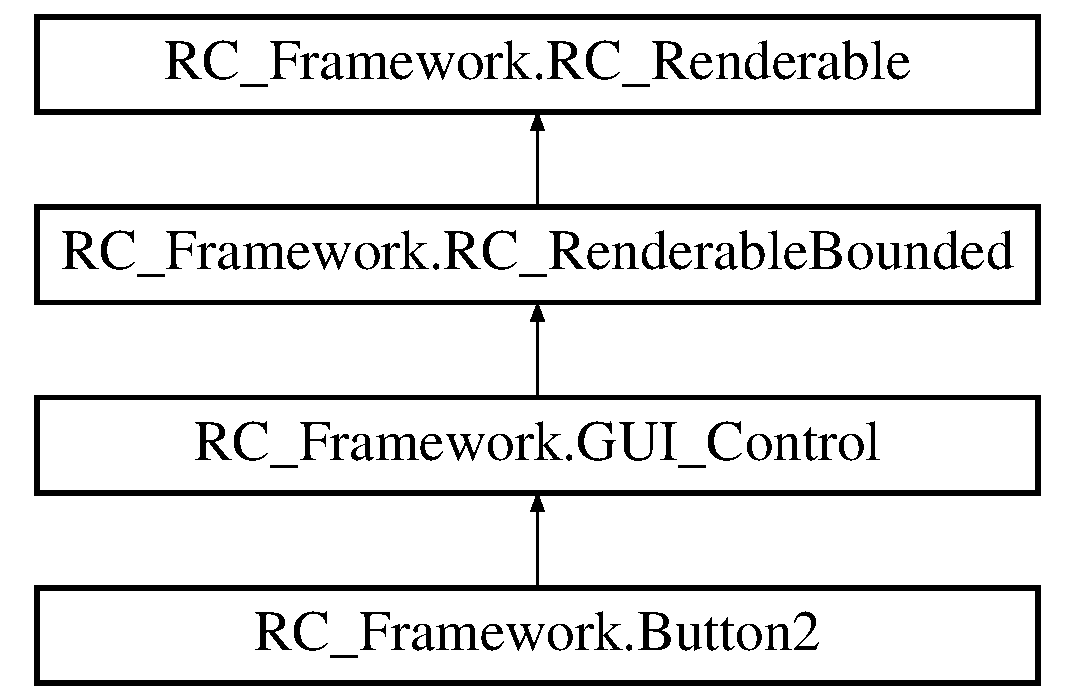
\includegraphics[height=4.000000cm]{class_r_c___framework_1_1_button2}
\end{center}
\end{figure}
\subsection*{Public Member Functions}
\begin{DoxyCompactItemize}
\item 
\mbox{\hyperlink{class_r_c___framework_1_1_button2_a59ba03059eb46cc321f6b38a0f5825ba}{Button2}} (Texture2D upZ, Texture2D downZ, Vector2 pos)
\begin{DoxyCompactList}\small\item\em \mbox{\hyperlink{class_r_c___framework_1_1_button2}{Button2}} constructor sizes to the texture \end{DoxyCompactList}\item 
\mbox{\hyperlink{class_r_c___framework_1_1_button2_a82157ea5fe77051daa5f1d6dae13566e}{Button2}} (Texture2D upZ, Texture2D downZ, Rectangle pos)
\begin{DoxyCompactList}\small\item\em \mbox{\hyperlink{class_r_c___framework_1_1_button2}{Button2}} constructor \end{DoxyCompactList}\item 
override void \mbox{\hyperlink{class_r_c___framework_1_1_button2_addc2770e16ca29d6bad27e7b234dddf3}{Draw}} (Sprite\+Batch sb)
\begin{DoxyCompactList}\small\item\em Draw yes a draw standard draw nothing more \end{DoxyCompactList}\item 
override bool \mbox{\hyperlink{class_r_c___framework_1_1_button2_ac15728fbc9e908a70990c159ecd5824f}{Mouse\+Down\+Event\+Left}} (float mouse\+\_\+x, float mouse\+\_\+y)
\begin{DoxyCompactList}\small\item\em the mouse clicks me \end{DoxyCompactList}\end{DoxyCompactItemize}
\subsection*{Public Attributes}
\begin{DoxyCompactItemize}
\item 
int \mbox{\hyperlink{class_r_c___framework_1_1_button2_a7b34b30866f790b3f0c5427bbeec5c91}{state}}
\begin{DoxyCompactList}\small\item\em current state 0=up 1=down \end{DoxyCompactList}\item 
bool \mbox{\hyperlink{class_r_c___framework_1_1_button2_abb085079359e47904684e34467809f00}{was\+Clicked}}
\begin{DoxyCompactList}\small\item\em true if clicked -\/ you poll this in update and once the click is actiopned you reset it \end{DoxyCompactList}\end{DoxyCompactItemize}
\subsection*{Additional Inherited Members}


\subsection{Detailed Description}
Simple Gui class with 2 images -\/ button up and button down 



\subsection{Constructor \& Destructor Documentation}
\mbox{\Hypertarget{class_r_c___framework_1_1_button2_a59ba03059eb46cc321f6b38a0f5825ba}\label{class_r_c___framework_1_1_button2_a59ba03059eb46cc321f6b38a0f5825ba}} 
\index{R\+C\+\_\+\+Framework\+::\+Button2@{R\+C\+\_\+\+Framework\+::\+Button2}!Button2@{Button2}}
\index{Button2@{Button2}!R\+C\+\_\+\+Framework\+::\+Button2@{R\+C\+\_\+\+Framework\+::\+Button2}}
\subsubsection{\texorpdfstring{Button2()}{Button2()}\hspace{0.1cm}{\footnotesize\ttfamily [1/2]}}
{\footnotesize\ttfamily R\+C\+\_\+\+Framework.\+Button2.\+Button2 (\begin{DoxyParamCaption}\item[{Texture2D}]{upZ,  }\item[{Texture2D}]{downZ,  }\item[{Vector2}]{pos }\end{DoxyParamCaption})}



\mbox{\hyperlink{class_r_c___framework_1_1_button2}{Button2}} constructor sizes to the texture 


\begin{DoxyParams}{Parameters}
{\em upZ} & \\
\hline
{\em downZ} & \\
\hline
{\em pos} & \\
\hline
\end{DoxyParams}
\mbox{\Hypertarget{class_r_c___framework_1_1_button2_a82157ea5fe77051daa5f1d6dae13566e}\label{class_r_c___framework_1_1_button2_a82157ea5fe77051daa5f1d6dae13566e}} 
\index{R\+C\+\_\+\+Framework\+::\+Button2@{R\+C\+\_\+\+Framework\+::\+Button2}!Button2@{Button2}}
\index{Button2@{Button2}!R\+C\+\_\+\+Framework\+::\+Button2@{R\+C\+\_\+\+Framework\+::\+Button2}}
\subsubsection{\texorpdfstring{Button2()}{Button2()}\hspace{0.1cm}{\footnotesize\ttfamily [2/2]}}
{\footnotesize\ttfamily R\+C\+\_\+\+Framework.\+Button2.\+Button2 (\begin{DoxyParamCaption}\item[{Texture2D}]{upZ,  }\item[{Texture2D}]{downZ,  }\item[{Rectangle}]{pos }\end{DoxyParamCaption})}



\mbox{\hyperlink{class_r_c___framework_1_1_button2}{Button2}} constructor 


\begin{DoxyParams}{Parameters}
{\em upZ} & \\
\hline
{\em downZ} & \\
\hline
{\em pos} & \\
\hline
\end{DoxyParams}


\subsection{Member Function Documentation}
\mbox{\Hypertarget{class_r_c___framework_1_1_button2_addc2770e16ca29d6bad27e7b234dddf3}\label{class_r_c___framework_1_1_button2_addc2770e16ca29d6bad27e7b234dddf3}} 
\index{R\+C\+\_\+\+Framework\+::\+Button2@{R\+C\+\_\+\+Framework\+::\+Button2}!Draw@{Draw}}
\index{Draw@{Draw}!R\+C\+\_\+\+Framework\+::\+Button2@{R\+C\+\_\+\+Framework\+::\+Button2}}
\subsubsection{\texorpdfstring{Draw()}{Draw()}}
{\footnotesize\ttfamily override void R\+C\+\_\+\+Framework.\+Button2.\+Draw (\begin{DoxyParamCaption}\item[{Sprite\+Batch}]{sb }\end{DoxyParamCaption})\hspace{0.3cm}{\ttfamily [virtual]}}



Draw yes a draw standard draw nothing more 


\begin{DoxyParams}{Parameters}
{\em sb} & \\
\hline
\end{DoxyParams}


Reimplemented from \mbox{\hyperlink{class_r_c___framework_1_1_r_c___renderable_acc26db34e382a25a989c4c0dd0354b23}{R\+C\+\_\+\+Framework.\+R\+C\+\_\+\+Renderable}}.

\mbox{\Hypertarget{class_r_c___framework_1_1_button2_ac15728fbc9e908a70990c159ecd5824f}\label{class_r_c___framework_1_1_button2_ac15728fbc9e908a70990c159ecd5824f}} 
\index{R\+C\+\_\+\+Framework\+::\+Button2@{R\+C\+\_\+\+Framework\+::\+Button2}!Mouse\+Down\+Event\+Left@{Mouse\+Down\+Event\+Left}}
\index{Mouse\+Down\+Event\+Left@{Mouse\+Down\+Event\+Left}!R\+C\+\_\+\+Framework\+::\+Button2@{R\+C\+\_\+\+Framework\+::\+Button2}}
\subsubsection{\texorpdfstring{Mouse\+Down\+Event\+Left()}{MouseDownEventLeft()}}
{\footnotesize\ttfamily override bool R\+C\+\_\+\+Framework.\+Button2.\+Mouse\+Down\+Event\+Left (\begin{DoxyParamCaption}\item[{float}]{mouse\+\_\+x,  }\item[{float}]{mouse\+\_\+y }\end{DoxyParamCaption})\hspace{0.3cm}{\ttfamily [virtual]}}



the mouse clicks me 


\begin{DoxyParams}{Parameters}
{\em mouse\+\_\+x} & \\
\hline
{\em mouse\+\_\+y} & \\
\hline
\end{DoxyParams}
\begin{DoxyReturn}{Returns}

\end{DoxyReturn}


Reimplemented from \mbox{\hyperlink{class_r_c___framework_1_1_g_u_i___control_a005e7f109afd21abd6576fdf70212af5}{R\+C\+\_\+\+Framework.\+G\+U\+I\+\_\+\+Control}}.



\subsection{Member Data Documentation}
\mbox{\Hypertarget{class_r_c___framework_1_1_button2_a7b34b30866f790b3f0c5427bbeec5c91}\label{class_r_c___framework_1_1_button2_a7b34b30866f790b3f0c5427bbeec5c91}} 
\index{R\+C\+\_\+\+Framework\+::\+Button2@{R\+C\+\_\+\+Framework\+::\+Button2}!state@{state}}
\index{state@{state}!R\+C\+\_\+\+Framework\+::\+Button2@{R\+C\+\_\+\+Framework\+::\+Button2}}
\subsubsection{\texorpdfstring{state}{state}}
{\footnotesize\ttfamily int R\+C\+\_\+\+Framework.\+Button2.\+state}



current state 0=up 1=down 

\mbox{\Hypertarget{class_r_c___framework_1_1_button2_abb085079359e47904684e34467809f00}\label{class_r_c___framework_1_1_button2_abb085079359e47904684e34467809f00}} 
\index{R\+C\+\_\+\+Framework\+::\+Button2@{R\+C\+\_\+\+Framework\+::\+Button2}!was\+Clicked@{was\+Clicked}}
\index{was\+Clicked@{was\+Clicked}!R\+C\+\_\+\+Framework\+::\+Button2@{R\+C\+\_\+\+Framework\+::\+Button2}}
\subsubsection{\texorpdfstring{was\+Clicked}{wasClicked}}
{\footnotesize\ttfamily bool R\+C\+\_\+\+Framework.\+Button2.\+was\+Clicked}



true if clicked -\/ you poll this in update and once the click is actiopned you reset it 



The documentation for this class was generated from the following file\+:\begin{DoxyCompactItemize}
\item 
F\+:/\+B/\+R\+C\+\_\+\+Framework2018/\+Source/\mbox{\hyperlink{_r_c___g_u_i_8cs}{R\+C\+\_\+\+G\+U\+I.\+cs}}\end{DoxyCompactItemize}

\hypertarget{class_r_c___framework_1_1_button_ann}{}\section{R\+C\+\_\+\+Framework.\+Button\+Ann Class Reference}
\label{class_r_c___framework_1_1_button_ann}\index{R\+C\+\_\+\+Framework.\+Button\+Ann@{R\+C\+\_\+\+Framework.\+Button\+Ann}}


A line of text in a frame so to speak the border will have illusion of 3D if its not pure black or white  


Inheritance diagram for R\+C\+\_\+\+Framework.\+Button\+Ann\+:\begin{figure}[H]
\begin{center}
\leavevmode
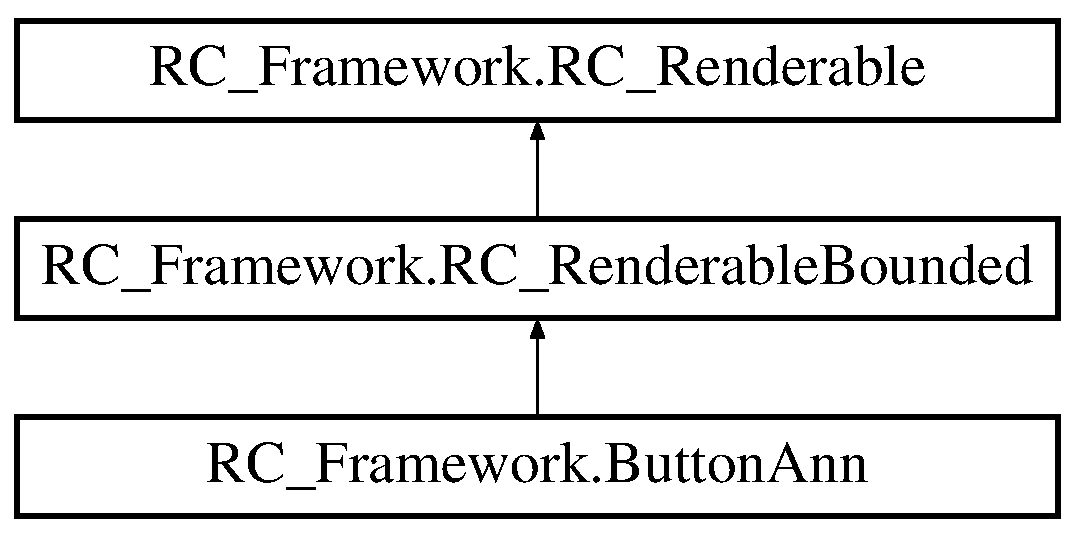
\includegraphics[height=3.000000cm]{class_r_c___framework_1_1_button_ann}
\end{center}
\end{figure}
\subsection*{Public Member Functions}
\begin{DoxyCompactItemize}
\item 
\mbox{\hyperlink{class_r_c___framework_1_1_button_ann_a8110236e18489fa16c2a760b0700aad4}{Button\+Ann}} (Texture2D back\+Ground\+Tex, string textZ, Sprite\+Font fontZ, Vector2 pos, Color font\+ColorZ, Color back\+Color)
\item 
override void \mbox{\hyperlink{class_r_c___framework_1_1_button_ann_ab513dd55d4cf3e1515761f0e4c5f9e44}{Draw}} (Sprite\+Batch sb)
\begin{DoxyCompactList}\small\item\em Standard draw routine which assumes the renderable knows where it is \end{DoxyCompactList}\item 
override bool \mbox{\hyperlink{class_r_c___framework_1_1_button_ann_a387c65413a4dbfd360cab56476fc21a4}{Mouse\+Over}} (float mouse\+\_\+x, float mouse\+\_\+y)
\end{DoxyCompactItemize}
\subsection*{Public Attributes}
\begin{DoxyCompactItemize}
\item 
Vector2 \mbox{\hyperlink{class_r_c___framework_1_1_button_ann_adf8a491a03cb62e48017ce118f216a6a}{text\+Offset}}
\end{DoxyCompactItemize}
\subsection*{Properties}
\begin{DoxyCompactItemize}
\item 
Sprite\+Font \mbox{\hyperlink{class_r_c___framework_1_1_button_ann_a2773c8d871d7d9eedb544cf1ad663f05}{font}}\hspace{0.3cm}{\ttfamily  \mbox{[}get, set\mbox{]}}
\item 
int \mbox{\hyperlink{class_r_c___framework_1_1_button_ann_aba404164b4906b9e067c7fb8a8188e4a}{kind}}\hspace{0.3cm}{\ttfamily  \mbox{[}get, set\mbox{]}}
\end{DoxyCompactItemize}
\subsection*{Additional Inherited Members}


\subsection{Detailed Description}
A line of text in a frame so to speak the border will have illusion of 3D if its not pure black or white 



\subsection{Constructor \& Destructor Documentation}
\mbox{\Hypertarget{class_r_c___framework_1_1_button_ann_a8110236e18489fa16c2a760b0700aad4}\label{class_r_c___framework_1_1_button_ann_a8110236e18489fa16c2a760b0700aad4}} 
\index{R\+C\+\_\+\+Framework\+::\+Button\+Ann@{R\+C\+\_\+\+Framework\+::\+Button\+Ann}!Button\+Ann@{Button\+Ann}}
\index{Button\+Ann@{Button\+Ann}!R\+C\+\_\+\+Framework\+::\+Button\+Ann@{R\+C\+\_\+\+Framework\+::\+Button\+Ann}}
\subsubsection{\texorpdfstring{Button\+Ann()}{ButtonAnn()}}
{\footnotesize\ttfamily R\+C\+\_\+\+Framework.\+Button\+Ann.\+Button\+Ann (\begin{DoxyParamCaption}\item[{Texture2D}]{back\+Ground\+Tex,  }\item[{string}]{textZ,  }\item[{Sprite\+Font}]{fontZ,  }\item[{Vector2}]{pos,  }\item[{Color}]{font\+ColorZ,  }\item[{Color}]{back\+Color }\end{DoxyParamCaption})}



\subsection{Member Function Documentation}
\mbox{\Hypertarget{class_r_c___framework_1_1_button_ann_ab513dd55d4cf3e1515761f0e4c5f9e44}\label{class_r_c___framework_1_1_button_ann_ab513dd55d4cf3e1515761f0e4c5f9e44}} 
\index{R\+C\+\_\+\+Framework\+::\+Button\+Ann@{R\+C\+\_\+\+Framework\+::\+Button\+Ann}!Draw@{Draw}}
\index{Draw@{Draw}!R\+C\+\_\+\+Framework\+::\+Button\+Ann@{R\+C\+\_\+\+Framework\+::\+Button\+Ann}}
\subsubsection{\texorpdfstring{Draw()}{Draw()}}
{\footnotesize\ttfamily override void R\+C\+\_\+\+Framework.\+Button\+Ann.\+Draw (\begin{DoxyParamCaption}\item[{Sprite\+Batch}]{sb }\end{DoxyParamCaption})\hspace{0.3cm}{\ttfamily [virtual]}}



Standard draw routine which assumes the renderable knows where it is 


\begin{DoxyParams}{Parameters}
{\em sb} & \\
\hline
\end{DoxyParams}


Reimplemented from \mbox{\hyperlink{class_r_c___framework_1_1_r_c___renderable_acc26db34e382a25a989c4c0dd0354b23}{R\+C\+\_\+\+Framework.\+R\+C\+\_\+\+Renderable}}.

\mbox{\Hypertarget{class_r_c___framework_1_1_button_ann_a387c65413a4dbfd360cab56476fc21a4}\label{class_r_c___framework_1_1_button_ann_a387c65413a4dbfd360cab56476fc21a4}} 
\index{R\+C\+\_\+\+Framework\+::\+Button\+Ann@{R\+C\+\_\+\+Framework\+::\+Button\+Ann}!Mouse\+Over@{Mouse\+Over}}
\index{Mouse\+Over@{Mouse\+Over}!R\+C\+\_\+\+Framework\+::\+Button\+Ann@{R\+C\+\_\+\+Framework\+::\+Button\+Ann}}
\subsubsection{\texorpdfstring{Mouse\+Over()}{MouseOver()}}
{\footnotesize\ttfamily override bool R\+C\+\_\+\+Framework.\+Button\+Ann.\+Mouse\+Over (\begin{DoxyParamCaption}\item[{float}]{mouse\+\_\+x,  }\item[{float}]{mouse\+\_\+y }\end{DoxyParamCaption})\hspace{0.3cm}{\ttfamily [virtual]}}



Reimplemented from \mbox{\hyperlink{class_r_c___framework_1_1_r_c___renderable_abd55ea96d88d7bd2207e3a4ede1f1a05}{R\+C\+\_\+\+Framework.\+R\+C\+\_\+\+Renderable}}.



\subsection{Member Data Documentation}
\mbox{\Hypertarget{class_r_c___framework_1_1_button_ann_adf8a491a03cb62e48017ce118f216a6a}\label{class_r_c___framework_1_1_button_ann_adf8a491a03cb62e48017ce118f216a6a}} 
\index{R\+C\+\_\+\+Framework\+::\+Button\+Ann@{R\+C\+\_\+\+Framework\+::\+Button\+Ann}!text\+Offset@{text\+Offset}}
\index{text\+Offset@{text\+Offset}!R\+C\+\_\+\+Framework\+::\+Button\+Ann@{R\+C\+\_\+\+Framework\+::\+Button\+Ann}}
\subsubsection{\texorpdfstring{text\+Offset}{textOffset}}
{\footnotesize\ttfamily Vector2 R\+C\+\_\+\+Framework.\+Button\+Ann.\+text\+Offset}



\subsection{Property Documentation}
\mbox{\Hypertarget{class_r_c___framework_1_1_button_ann_a2773c8d871d7d9eedb544cf1ad663f05}\label{class_r_c___framework_1_1_button_ann_a2773c8d871d7d9eedb544cf1ad663f05}} 
\index{R\+C\+\_\+\+Framework\+::\+Button\+Ann@{R\+C\+\_\+\+Framework\+::\+Button\+Ann}!font@{font}}
\index{font@{font}!R\+C\+\_\+\+Framework\+::\+Button\+Ann@{R\+C\+\_\+\+Framework\+::\+Button\+Ann}}
\subsubsection{\texorpdfstring{font}{font}}
{\footnotesize\ttfamily Sprite\+Font R\+C\+\_\+\+Framework.\+Button\+Ann.\+font\hspace{0.3cm}{\ttfamily [get]}, {\ttfamily [set]}}

\mbox{\Hypertarget{class_r_c___framework_1_1_button_ann_aba404164b4906b9e067c7fb8a8188e4a}\label{class_r_c___framework_1_1_button_ann_aba404164b4906b9e067c7fb8a8188e4a}} 
\index{R\+C\+\_\+\+Framework\+::\+Button\+Ann@{R\+C\+\_\+\+Framework\+::\+Button\+Ann}!kind@{kind}}
\index{kind@{kind}!R\+C\+\_\+\+Framework\+::\+Button\+Ann@{R\+C\+\_\+\+Framework\+::\+Button\+Ann}}
\subsubsection{\texorpdfstring{kind}{kind}}
{\footnotesize\ttfamily int R\+C\+\_\+\+Framework.\+Button\+Ann.\+kind\hspace{0.3cm}{\ttfamily [get]}, {\ttfamily [set]}}



The documentation for this class was generated from the following file\+:\begin{DoxyCompactItemize}
\item 
F\+:/\+B/\+R\+C\+\_\+\+Framework2018/\+Source/\mbox{\hyperlink{_r_c___renderable_bounded_8cs}{R\+C\+\_\+\+Renderable\+Bounded.\+cs}}\end{DoxyCompactItemize}

\hypertarget{class_r_c___framework_1_1_button_s_i}{}\section{R\+C\+\_\+\+Framework.\+Button\+SI Class Reference}
\label{class_r_c___framework_1_1_button_s_i}\index{R\+C\+\_\+\+Framework.\+Button\+SI@{R\+C\+\_\+\+Framework.\+Button\+SI}}


\mbox{\hyperlink{class_r_c___framework_1_1_button_s_i}{Button\+SI}} Simple Gui button with 1 image but two colours to show when clicked  


Inheritance diagram for R\+C\+\_\+\+Framework.\+Button\+SI\+:\begin{figure}[H]
\begin{center}
\leavevmode
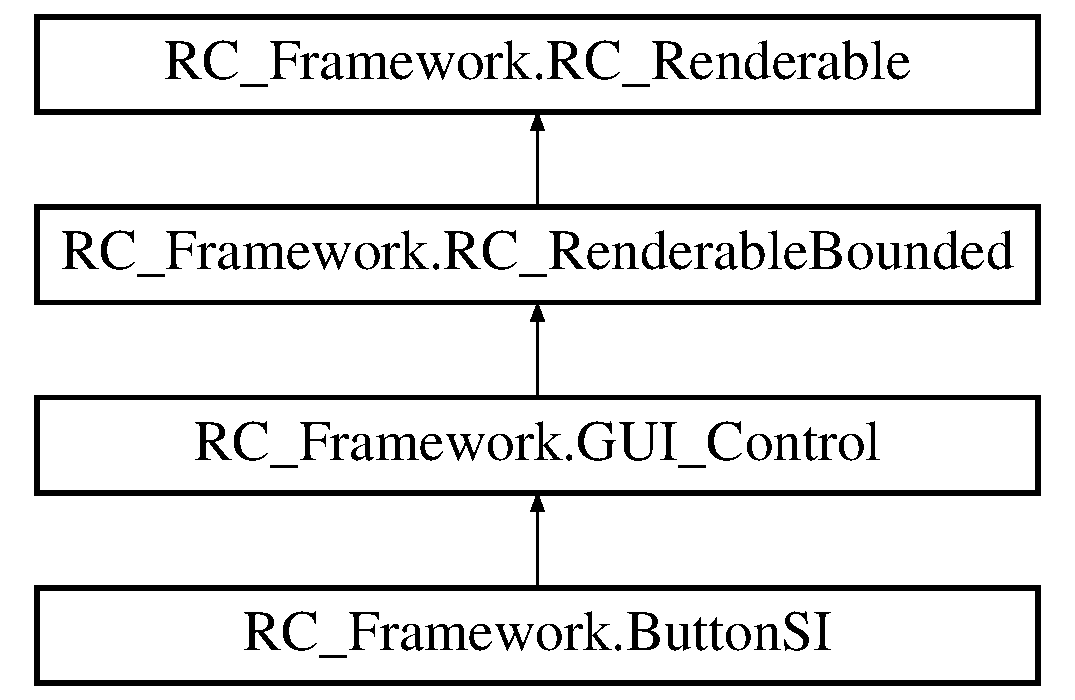
\includegraphics[height=4.000000cm]{class_r_c___framework_1_1_button_s_i}
\end{center}
\end{figure}
\subsection*{Public Member Functions}
\begin{DoxyCompactItemize}
\item 
\mbox{\hyperlink{class_r_c___framework_1_1_button_s_i_af419ab3d1513150939d673226bb4b3c8}{Button\+SI}} (Texture2D upZ, Color c\+Clicked, Vector2 pos)
\begin{DoxyCompactList}\small\item\em \mbox{\hyperlink{class_r_c___framework_1_1_button_s_i}{Button\+SI}} Constructor -\/ resizes to texture \end{DoxyCompactList}\item 
\mbox{\hyperlink{class_r_c___framework_1_1_button_s_i_aa1e864edccf775be2a5e87d1ac02b89a}{Button\+SI}} (Texture2D upZ, Color c\+Clicked, Rectangle pos)
\begin{DoxyCompactList}\small\item\em \mbox{\hyperlink{class_r_c___framework_1_1_button_s_i}{Button\+SI}} Constructor \end{DoxyCompactList}\item 
void \mbox{\hyperlink{class_r_c___framework_1_1_button_s_i_a4e0e489ebc76dd36dd5a6f0750dbe78b}{set\+Text}} (String t, Sprite\+Font f)
\begin{DoxyCompactList}\small\item\em set the text and font \end{DoxyCompactList}\item 
override void \mbox{\hyperlink{class_r_c___framework_1_1_button_s_i_a9527749f48994c13be5b72b2cb370b29}{Draw}} (Sprite\+Batch sb)
\begin{DoxyCompactList}\small\item\em Draw draw draw B\+O\+R\+E\+I\+NG \end{DoxyCompactList}\item 
override bool \mbox{\hyperlink{class_r_c___framework_1_1_button_s_i_a4323f8436749655b240fa35caa15daa6}{Mouse\+Down\+Event\+Left}} (float mouse\+\_\+x, float mouse\+\_\+y)
\begin{DoxyCompactList}\small\item\em Handle mouse click \end{DoxyCompactList}\item 
override void \mbox{\hyperlink{class_r_c___framework_1_1_button_s_i_a28efd8765e3ec06c727477352d1e5c01}{Update}} (Game\+Time game\+Time)
\begin{DoxyCompactList}\small\item\em straightforward Update \end{DoxyCompactList}\end{DoxyCompactItemize}
\subsection*{Public Attributes}
\begin{DoxyCompactItemize}
\item 
int \mbox{\hyperlink{class_r_c___framework_1_1_button_s_i_a7276e83d5155487cc26b770d71beab2c}{state}}
\begin{DoxyCompactList}\small\item\em 0=up 1=down \end{DoxyCompactList}\item 
bool \mbox{\hyperlink{class_r_c___framework_1_1_button_s_i_af137c098b87fc391e613d52ba00db7e4}{was\+Clicked}}
\begin{DoxyCompactList}\small\item\em true if clicked -\/ you poll this in update and once the click is actiopned you reset it \end{DoxyCompactList}\item 
int \mbox{\hyperlink{class_r_c___framework_1_1_button_s_i_af149eec1943e7fc1e6602bf0bb81af57}{click\+Time\+Max}} = 30
\begin{DoxyCompactList}\small\item\em Time in ticks to show click \end{DoxyCompactList}\item 
String \mbox{\hyperlink{class_r_c___framework_1_1_button_s_i_a8269aae4c3e59b9b784ce4f0bcd092a7}{Text\+To\+Display}} =\char`\"{}\char`\"{}
\begin{DoxyCompactList}\small\item\em Optional text string \end{DoxyCompactList}\item 
Sprite\+Font \mbox{\hyperlink{class_r_c___framework_1_1_button_s_i_a9e1b4799a8570e57594d051479ead0f0}{tfont}}
\begin{DoxyCompactList}\small\item\em Font to display text \end{DoxyCompactList}\item 
Vector2 \mbox{\hyperlink{class_r_c___framework_1_1_button_s_i_a829f3c4b72f84fcecb06422f526d5c86}{text\+Offset}} = new Vector2(5, 3)
\begin{DoxyCompactList}\small\item\em Where to show the text \end{DoxyCompactList}\end{DoxyCompactItemize}
\subsection*{Additional Inherited Members}


\subsection{Detailed Description}
\mbox{\hyperlink{class_r_c___framework_1_1_button_s_i}{Button\+SI}} Simple Gui button with 1 image but two colours to show when clicked 



\subsection{Constructor \& Destructor Documentation}
\mbox{\Hypertarget{class_r_c___framework_1_1_button_s_i_af419ab3d1513150939d673226bb4b3c8}\label{class_r_c___framework_1_1_button_s_i_af419ab3d1513150939d673226bb4b3c8}} 
\index{R\+C\+\_\+\+Framework\+::\+Button\+SI@{R\+C\+\_\+\+Framework\+::\+Button\+SI}!Button\+SI@{Button\+SI}}
\index{Button\+SI@{Button\+SI}!R\+C\+\_\+\+Framework\+::\+Button\+SI@{R\+C\+\_\+\+Framework\+::\+Button\+SI}}
\subsubsection{\texorpdfstring{Button\+S\+I()}{ButtonSI()}\hspace{0.1cm}{\footnotesize\ttfamily [1/2]}}
{\footnotesize\ttfamily R\+C\+\_\+\+Framework.\+Button\+S\+I.\+Button\+SI (\begin{DoxyParamCaption}\item[{Texture2D}]{upZ,  }\item[{Color}]{c\+Clicked,  }\item[{Vector2}]{pos }\end{DoxyParamCaption})}



\mbox{\hyperlink{class_r_c___framework_1_1_button_s_i}{Button\+SI}} Constructor -\/ resizes to texture 


\begin{DoxyParams}{Parameters}
{\em upZ} & \\
\hline
{\em c\+Clicked} & \\
\hline
{\em pos} & \\
\hline
\end{DoxyParams}
\mbox{\Hypertarget{class_r_c___framework_1_1_button_s_i_aa1e864edccf775be2a5e87d1ac02b89a}\label{class_r_c___framework_1_1_button_s_i_aa1e864edccf775be2a5e87d1ac02b89a}} 
\index{R\+C\+\_\+\+Framework\+::\+Button\+SI@{R\+C\+\_\+\+Framework\+::\+Button\+SI}!Button\+SI@{Button\+SI}}
\index{Button\+SI@{Button\+SI}!R\+C\+\_\+\+Framework\+::\+Button\+SI@{R\+C\+\_\+\+Framework\+::\+Button\+SI}}
\subsubsection{\texorpdfstring{Button\+S\+I()}{ButtonSI()}\hspace{0.1cm}{\footnotesize\ttfamily [2/2]}}
{\footnotesize\ttfamily R\+C\+\_\+\+Framework.\+Button\+S\+I.\+Button\+SI (\begin{DoxyParamCaption}\item[{Texture2D}]{upZ,  }\item[{Color}]{c\+Clicked,  }\item[{Rectangle}]{pos }\end{DoxyParamCaption})}



\mbox{\hyperlink{class_r_c___framework_1_1_button_s_i}{Button\+SI}} Constructor 


\begin{DoxyParams}{Parameters}
{\em upZ} & \\
\hline
{\em c\+Clicked} & \\
\hline
{\em pos} & \\
\hline
\end{DoxyParams}


\subsection{Member Function Documentation}
\mbox{\Hypertarget{class_r_c___framework_1_1_button_s_i_a9527749f48994c13be5b72b2cb370b29}\label{class_r_c___framework_1_1_button_s_i_a9527749f48994c13be5b72b2cb370b29}} 
\index{R\+C\+\_\+\+Framework\+::\+Button\+SI@{R\+C\+\_\+\+Framework\+::\+Button\+SI}!Draw@{Draw}}
\index{Draw@{Draw}!R\+C\+\_\+\+Framework\+::\+Button\+SI@{R\+C\+\_\+\+Framework\+::\+Button\+SI}}
\subsubsection{\texorpdfstring{Draw()}{Draw()}}
{\footnotesize\ttfamily override void R\+C\+\_\+\+Framework.\+Button\+S\+I.\+Draw (\begin{DoxyParamCaption}\item[{Sprite\+Batch}]{sb }\end{DoxyParamCaption})\hspace{0.3cm}{\ttfamily [virtual]}}



Draw draw draw B\+O\+R\+E\+I\+NG 


\begin{DoxyParams}{Parameters}
{\em sb} & \\
\hline
\end{DoxyParams}


Reimplemented from \mbox{\hyperlink{class_r_c___framework_1_1_r_c___renderable_acc26db34e382a25a989c4c0dd0354b23}{R\+C\+\_\+\+Framework.\+R\+C\+\_\+\+Renderable}}.

\mbox{\Hypertarget{class_r_c___framework_1_1_button_s_i_a4323f8436749655b240fa35caa15daa6}\label{class_r_c___framework_1_1_button_s_i_a4323f8436749655b240fa35caa15daa6}} 
\index{R\+C\+\_\+\+Framework\+::\+Button\+SI@{R\+C\+\_\+\+Framework\+::\+Button\+SI}!Mouse\+Down\+Event\+Left@{Mouse\+Down\+Event\+Left}}
\index{Mouse\+Down\+Event\+Left@{Mouse\+Down\+Event\+Left}!R\+C\+\_\+\+Framework\+::\+Button\+SI@{R\+C\+\_\+\+Framework\+::\+Button\+SI}}
\subsubsection{\texorpdfstring{Mouse\+Down\+Event\+Left()}{MouseDownEventLeft()}}
{\footnotesize\ttfamily override bool R\+C\+\_\+\+Framework.\+Button\+S\+I.\+Mouse\+Down\+Event\+Left (\begin{DoxyParamCaption}\item[{float}]{mouse\+\_\+x,  }\item[{float}]{mouse\+\_\+y }\end{DoxyParamCaption})\hspace{0.3cm}{\ttfamily [virtual]}}



Handle mouse click 


\begin{DoxyParams}{Parameters}
{\em mouse\+\_\+x} & \\
\hline
{\em mouse\+\_\+y} & \\
\hline
\end{DoxyParams}
\begin{DoxyReturn}{Returns}

\end{DoxyReturn}


Reimplemented from \mbox{\hyperlink{class_r_c___framework_1_1_g_u_i___control_a005e7f109afd21abd6576fdf70212af5}{R\+C\+\_\+\+Framework.\+G\+U\+I\+\_\+\+Control}}.

\mbox{\Hypertarget{class_r_c___framework_1_1_button_s_i_a4e0e489ebc76dd36dd5a6f0750dbe78b}\label{class_r_c___framework_1_1_button_s_i_a4e0e489ebc76dd36dd5a6f0750dbe78b}} 
\index{R\+C\+\_\+\+Framework\+::\+Button\+SI@{R\+C\+\_\+\+Framework\+::\+Button\+SI}!set\+Text@{set\+Text}}
\index{set\+Text@{set\+Text}!R\+C\+\_\+\+Framework\+::\+Button\+SI@{R\+C\+\_\+\+Framework\+::\+Button\+SI}}
\subsubsection{\texorpdfstring{set\+Text()}{setText()}}
{\footnotesize\ttfamily void R\+C\+\_\+\+Framework.\+Button\+S\+I.\+set\+Text (\begin{DoxyParamCaption}\item[{String}]{t,  }\item[{Sprite\+Font}]{f }\end{DoxyParamCaption})}



set the text and font 


\begin{DoxyParams}{Parameters}
{\em t} & \\
\hline
{\em f} & \\
\hline
\end{DoxyParams}
\mbox{\Hypertarget{class_r_c___framework_1_1_button_s_i_a28efd8765e3ec06c727477352d1e5c01}\label{class_r_c___framework_1_1_button_s_i_a28efd8765e3ec06c727477352d1e5c01}} 
\index{R\+C\+\_\+\+Framework\+::\+Button\+SI@{R\+C\+\_\+\+Framework\+::\+Button\+SI}!Update@{Update}}
\index{Update@{Update}!R\+C\+\_\+\+Framework\+::\+Button\+SI@{R\+C\+\_\+\+Framework\+::\+Button\+SI}}
\subsubsection{\texorpdfstring{Update()}{Update()}}
{\footnotesize\ttfamily override void R\+C\+\_\+\+Framework.\+Button\+S\+I.\+Update (\begin{DoxyParamCaption}\item[{Game\+Time}]{game\+Time }\end{DoxyParamCaption})\hspace{0.3cm}{\ttfamily [virtual]}}



straightforward Update 


\begin{DoxyParams}{Parameters}
{\em game\+Time} & \\
\hline
\end{DoxyParams}


Reimplemented from \mbox{\hyperlink{class_r_c___framework_1_1_g_u_i___control_a7aa3b0b6ba141d995ca830ff99ae3003}{R\+C\+\_\+\+Framework.\+G\+U\+I\+\_\+\+Control}}.



\subsection{Member Data Documentation}
\mbox{\Hypertarget{class_r_c___framework_1_1_button_s_i_af149eec1943e7fc1e6602bf0bb81af57}\label{class_r_c___framework_1_1_button_s_i_af149eec1943e7fc1e6602bf0bb81af57}} 
\index{R\+C\+\_\+\+Framework\+::\+Button\+SI@{R\+C\+\_\+\+Framework\+::\+Button\+SI}!click\+Time\+Max@{click\+Time\+Max}}
\index{click\+Time\+Max@{click\+Time\+Max}!R\+C\+\_\+\+Framework\+::\+Button\+SI@{R\+C\+\_\+\+Framework\+::\+Button\+SI}}
\subsubsection{\texorpdfstring{click\+Time\+Max}{clickTimeMax}}
{\footnotesize\ttfamily int R\+C\+\_\+\+Framework.\+Button\+S\+I.\+click\+Time\+Max = 30}



Time in ticks to show click 

\mbox{\Hypertarget{class_r_c___framework_1_1_button_s_i_a7276e83d5155487cc26b770d71beab2c}\label{class_r_c___framework_1_1_button_s_i_a7276e83d5155487cc26b770d71beab2c}} 
\index{R\+C\+\_\+\+Framework\+::\+Button\+SI@{R\+C\+\_\+\+Framework\+::\+Button\+SI}!state@{state}}
\index{state@{state}!R\+C\+\_\+\+Framework\+::\+Button\+SI@{R\+C\+\_\+\+Framework\+::\+Button\+SI}}
\subsubsection{\texorpdfstring{state}{state}}
{\footnotesize\ttfamily int R\+C\+\_\+\+Framework.\+Button\+S\+I.\+state}



0=up 1=down 

\mbox{\Hypertarget{class_r_c___framework_1_1_button_s_i_a829f3c4b72f84fcecb06422f526d5c86}\label{class_r_c___framework_1_1_button_s_i_a829f3c4b72f84fcecb06422f526d5c86}} 
\index{R\+C\+\_\+\+Framework\+::\+Button\+SI@{R\+C\+\_\+\+Framework\+::\+Button\+SI}!text\+Offset@{text\+Offset}}
\index{text\+Offset@{text\+Offset}!R\+C\+\_\+\+Framework\+::\+Button\+SI@{R\+C\+\_\+\+Framework\+::\+Button\+SI}}
\subsubsection{\texorpdfstring{text\+Offset}{textOffset}}
{\footnotesize\ttfamily Vector2 R\+C\+\_\+\+Framework.\+Button\+S\+I.\+text\+Offset = new Vector2(5, 3)}



Where to show the text 

\mbox{\Hypertarget{class_r_c___framework_1_1_button_s_i_a8269aae4c3e59b9b784ce4f0bcd092a7}\label{class_r_c___framework_1_1_button_s_i_a8269aae4c3e59b9b784ce4f0bcd092a7}} 
\index{R\+C\+\_\+\+Framework\+::\+Button\+SI@{R\+C\+\_\+\+Framework\+::\+Button\+SI}!Text\+To\+Display@{Text\+To\+Display}}
\index{Text\+To\+Display@{Text\+To\+Display}!R\+C\+\_\+\+Framework\+::\+Button\+SI@{R\+C\+\_\+\+Framework\+::\+Button\+SI}}
\subsubsection{\texorpdfstring{Text\+To\+Display}{TextToDisplay}}
{\footnotesize\ttfamily String R\+C\+\_\+\+Framework.\+Button\+S\+I.\+Text\+To\+Display =\char`\"{}\char`\"{}}



Optional text string 

\mbox{\Hypertarget{class_r_c___framework_1_1_button_s_i_a9e1b4799a8570e57594d051479ead0f0}\label{class_r_c___framework_1_1_button_s_i_a9e1b4799a8570e57594d051479ead0f0}} 
\index{R\+C\+\_\+\+Framework\+::\+Button\+SI@{R\+C\+\_\+\+Framework\+::\+Button\+SI}!tfont@{tfont}}
\index{tfont@{tfont}!R\+C\+\_\+\+Framework\+::\+Button\+SI@{R\+C\+\_\+\+Framework\+::\+Button\+SI}}
\subsubsection{\texorpdfstring{tfont}{tfont}}
{\footnotesize\ttfamily Sprite\+Font R\+C\+\_\+\+Framework.\+Button\+S\+I.\+tfont}



Font to display text 

\mbox{\Hypertarget{class_r_c___framework_1_1_button_s_i_af137c098b87fc391e613d52ba00db7e4}\label{class_r_c___framework_1_1_button_s_i_af137c098b87fc391e613d52ba00db7e4}} 
\index{R\+C\+\_\+\+Framework\+::\+Button\+SI@{R\+C\+\_\+\+Framework\+::\+Button\+SI}!was\+Clicked@{was\+Clicked}}
\index{was\+Clicked@{was\+Clicked}!R\+C\+\_\+\+Framework\+::\+Button\+SI@{R\+C\+\_\+\+Framework\+::\+Button\+SI}}
\subsubsection{\texorpdfstring{was\+Clicked}{wasClicked}}
{\footnotesize\ttfamily bool R\+C\+\_\+\+Framework.\+Button\+S\+I.\+was\+Clicked}



true if clicked -\/ you poll this in update and once the click is actiopned you reset it 



The documentation for this class was generated from the following file\+:\begin{DoxyCompactItemize}
\item 
F\+:/\+B/\+R\+C\+\_\+\+Framework2018/\+Source/\mbox{\hyperlink{_r_c___g_u_i_8cs}{R\+C\+\_\+\+G\+U\+I.\+cs}}\end{DoxyCompactItemize}

\hypertarget{class_r_c___framework_1_1_circle_fade}{}\section{R\+C\+\_\+\+Framework.\+Circle\+Fade Class Reference}
\label{class_r_c___framework_1_1_circle_fade}\index{R\+C\+\_\+\+Framework.\+Circle\+Fade@{R\+C\+\_\+\+Framework.\+Circle\+Fade}}


Fades and resizes a circle At end it can loop , go inactive or reverse its a fairly sophisticated tool usable for a lot of diferent eye candy effects remeber to run update  


Inheritance diagram for R\+C\+\_\+\+Framework.\+Circle\+Fade\+:\begin{figure}[H]
\begin{center}
\leavevmode
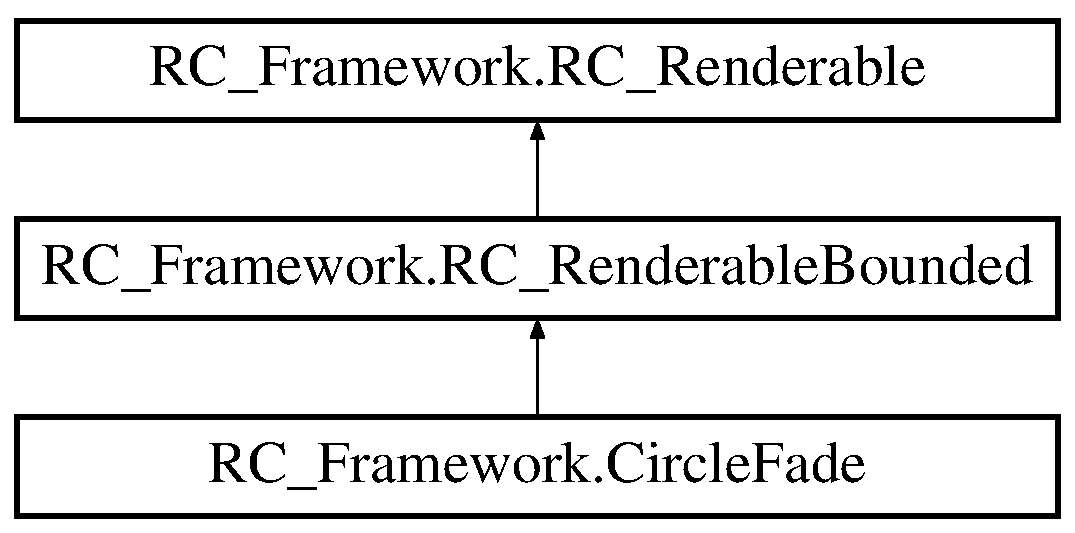
\includegraphics[height=3.000000cm]{class_r_c___framework_1_1_circle_fade}
\end{center}
\end{figure}
\subsection*{Public Member Functions}
\begin{DoxyCompactItemize}
\item 
\mbox{\hyperlink{class_r_c___framework_1_1_circle_fade_af5b020dad42c77795b9c92808f019dfe}{Circle\+Fade}} (Vector2 init\+PositionZ, Vector2 final\+PositionZ, float init\+RadiusZ, float final\+RadiusZ, Color init\+ColourZ, Color final\+ColourZ, int fade\+TicksZ)
\item 
void \mbox{\hyperlink{class_r_c___framework_1_1_circle_fade_a98d6a3fd33cbe0c616813a1bad1cf6b7}{set\+Loop}} (int loopQ)
\item 
override void \mbox{\hyperlink{class_r_c___framework_1_1_circle_fade_a75194b070e20dab4a4720c9ba43ae5ab}{Draw}} (Sprite\+Batch sb)
\begin{DoxyCompactList}\small\item\em Standard draw routine which assumes the renderable knows where it is \end{DoxyCompactList}\item 
override void \mbox{\hyperlink{class_r_c___framework_1_1_circle_fade_ade4928b94a3b49c0d3ffbd43d37060e6}{Update}} (Game\+Time game\+Time)
\item 
override void \mbox{\hyperlink{class_r_c___framework_1_1_circle_fade_a7dd68138bc5eb6e9e6f2d031d9091a8a}{reset}} ()
\end{DoxyCompactItemize}
\subsection*{Public Attributes}
\begin{DoxyCompactItemize}
\item 
int \mbox{\hyperlink{class_r_c___framework_1_1_circle_fade_a3a0b913d580633476d9d6c78a5054c69}{loop}}
\end{DoxyCompactItemize}
\subsection*{Additional Inherited Members}


\subsection{Detailed Description}
Fades and resizes a circle At end it can loop , go inactive or reverse its a fairly sophisticated tool usable for a lot of diferent eye candy effects remeber to run update 



\subsection{Constructor \& Destructor Documentation}
\mbox{\Hypertarget{class_r_c___framework_1_1_circle_fade_af5b020dad42c77795b9c92808f019dfe}\label{class_r_c___framework_1_1_circle_fade_af5b020dad42c77795b9c92808f019dfe}} 
\index{R\+C\+\_\+\+Framework\+::\+Circle\+Fade@{R\+C\+\_\+\+Framework\+::\+Circle\+Fade}!Circle\+Fade@{Circle\+Fade}}
\index{Circle\+Fade@{Circle\+Fade}!R\+C\+\_\+\+Framework\+::\+Circle\+Fade@{R\+C\+\_\+\+Framework\+::\+Circle\+Fade}}
\subsubsection{\texorpdfstring{Circle\+Fade()}{CircleFade()}}
{\footnotesize\ttfamily R\+C\+\_\+\+Framework.\+Circle\+Fade.\+Circle\+Fade (\begin{DoxyParamCaption}\item[{Vector2}]{init\+PositionZ,  }\item[{Vector2}]{final\+PositionZ,  }\item[{float}]{init\+RadiusZ,  }\item[{float}]{final\+RadiusZ,  }\item[{Color}]{init\+ColourZ,  }\item[{Color}]{final\+ColourZ,  }\item[{int}]{fade\+TicksZ }\end{DoxyParamCaption})}



\subsection{Member Function Documentation}
\mbox{\Hypertarget{class_r_c___framework_1_1_circle_fade_a75194b070e20dab4a4720c9ba43ae5ab}\label{class_r_c___framework_1_1_circle_fade_a75194b070e20dab4a4720c9ba43ae5ab}} 
\index{R\+C\+\_\+\+Framework\+::\+Circle\+Fade@{R\+C\+\_\+\+Framework\+::\+Circle\+Fade}!Draw@{Draw}}
\index{Draw@{Draw}!R\+C\+\_\+\+Framework\+::\+Circle\+Fade@{R\+C\+\_\+\+Framework\+::\+Circle\+Fade}}
\subsubsection{\texorpdfstring{Draw()}{Draw()}}
{\footnotesize\ttfamily override void R\+C\+\_\+\+Framework.\+Circle\+Fade.\+Draw (\begin{DoxyParamCaption}\item[{Sprite\+Batch}]{sb }\end{DoxyParamCaption})\hspace{0.3cm}{\ttfamily [virtual]}}



Standard draw routine which assumes the renderable knows where it is 


\begin{DoxyParams}{Parameters}
{\em sb} & \\
\hline
\end{DoxyParams}


Reimplemented from \mbox{\hyperlink{class_r_c___framework_1_1_r_c___renderable_acc26db34e382a25a989c4c0dd0354b23}{R\+C\+\_\+\+Framework.\+R\+C\+\_\+\+Renderable}}.

\mbox{\Hypertarget{class_r_c___framework_1_1_circle_fade_a7dd68138bc5eb6e9e6f2d031d9091a8a}\label{class_r_c___framework_1_1_circle_fade_a7dd68138bc5eb6e9e6f2d031d9091a8a}} 
\index{R\+C\+\_\+\+Framework\+::\+Circle\+Fade@{R\+C\+\_\+\+Framework\+::\+Circle\+Fade}!reset@{reset}}
\index{reset@{reset}!R\+C\+\_\+\+Framework\+::\+Circle\+Fade@{R\+C\+\_\+\+Framework\+::\+Circle\+Fade}}
\subsubsection{\texorpdfstring{reset()}{reset()}}
{\footnotesize\ttfamily override void R\+C\+\_\+\+Framework.\+Circle\+Fade.\+reset (\begin{DoxyParamCaption}{ }\end{DoxyParamCaption})\hspace{0.3cm}{\ttfamily [virtual]}}



Reimplemented from \mbox{\hyperlink{class_r_c___framework_1_1_r_c___renderable_ae65ce69704d15963789f421b58618b1f}{R\+C\+\_\+\+Framework.\+R\+C\+\_\+\+Renderable}}.

\mbox{\Hypertarget{class_r_c___framework_1_1_circle_fade_a98d6a3fd33cbe0c616813a1bad1cf6b7}\label{class_r_c___framework_1_1_circle_fade_a98d6a3fd33cbe0c616813a1bad1cf6b7}} 
\index{R\+C\+\_\+\+Framework\+::\+Circle\+Fade@{R\+C\+\_\+\+Framework\+::\+Circle\+Fade}!set\+Loop@{set\+Loop}}
\index{set\+Loop@{set\+Loop}!R\+C\+\_\+\+Framework\+::\+Circle\+Fade@{R\+C\+\_\+\+Framework\+::\+Circle\+Fade}}
\subsubsection{\texorpdfstring{set\+Loop()}{setLoop()}}
{\footnotesize\ttfamily void R\+C\+\_\+\+Framework.\+Circle\+Fade.\+set\+Loop (\begin{DoxyParamCaption}\item[{int}]{loopQ }\end{DoxyParamCaption})}

\mbox{\Hypertarget{class_r_c___framework_1_1_circle_fade_ade4928b94a3b49c0d3ffbd43d37060e6}\label{class_r_c___framework_1_1_circle_fade_ade4928b94a3b49c0d3ffbd43d37060e6}} 
\index{R\+C\+\_\+\+Framework\+::\+Circle\+Fade@{R\+C\+\_\+\+Framework\+::\+Circle\+Fade}!Update@{Update}}
\index{Update@{Update}!R\+C\+\_\+\+Framework\+::\+Circle\+Fade@{R\+C\+\_\+\+Framework\+::\+Circle\+Fade}}
\subsubsection{\texorpdfstring{Update()}{Update()}}
{\footnotesize\ttfamily override void R\+C\+\_\+\+Framework.\+Circle\+Fade.\+Update (\begin{DoxyParamCaption}\item[{Game\+Time}]{game\+Time }\end{DoxyParamCaption})\hspace{0.3cm}{\ttfamily [virtual]}}



Reimplemented from \mbox{\hyperlink{class_r_c___framework_1_1_r_c___renderable_a5745bedc7ba0587aa1e1d8563c357228}{R\+C\+\_\+\+Framework.\+R\+C\+\_\+\+Renderable}}.



\subsection{Member Data Documentation}
\mbox{\Hypertarget{class_r_c___framework_1_1_circle_fade_a3a0b913d580633476d9d6c78a5054c69}\label{class_r_c___framework_1_1_circle_fade_a3a0b913d580633476d9d6c78a5054c69}} 
\index{R\+C\+\_\+\+Framework\+::\+Circle\+Fade@{R\+C\+\_\+\+Framework\+::\+Circle\+Fade}!loop@{loop}}
\index{loop@{loop}!R\+C\+\_\+\+Framework\+::\+Circle\+Fade@{R\+C\+\_\+\+Framework\+::\+Circle\+Fade}}
\subsubsection{\texorpdfstring{loop}{loop}}
{\footnotesize\ttfamily int R\+C\+\_\+\+Framework.\+Circle\+Fade.\+loop}



The documentation for this class was generated from the following file\+:\begin{DoxyCompactItemize}
\item 
F\+:/\+B/\+R\+C\+\_\+\+Framework2018/\+Source/\mbox{\hyperlink{_r_c___renderable_bounded_8cs}{R\+C\+\_\+\+Renderable\+Bounded.\+cs}}\end{DoxyCompactItemize}

\hypertarget{class_r_c___framework_1_1_color_field}{}\section{R\+C\+\_\+\+Framework.\+Color\+Field Class Reference}
\label{class_r_c___framework_1_1_color_field}\index{R\+C\+\_\+\+Framework.\+Color\+Field@{R\+C\+\_\+\+Framework.\+Color\+Field}}


This renderable is just a single rectangle of one colour, it requires that linebatch has been initialised  


Inheritance diagram for R\+C\+\_\+\+Framework.\+Color\+Field\+:\begin{figure}[H]
\begin{center}
\leavevmode
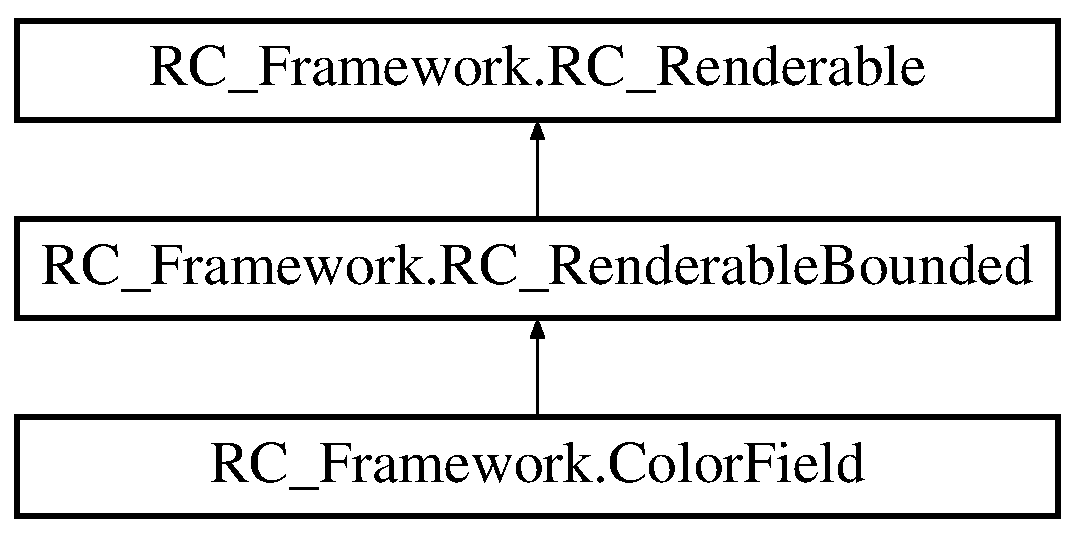
\includegraphics[height=3.000000cm]{class_r_c___framework_1_1_color_field}
\end{center}
\end{figure}
\subsection*{Public Member Functions}
\begin{DoxyCompactItemize}
\item 
\mbox{\hyperlink{class_r_c___framework_1_1_color_field_a57a40b1e28053b1b8482a4aef40dcd4d}{Color\+Field}} (Color c, Rectangle r)
\item 
override void \mbox{\hyperlink{class_r_c___framework_1_1_color_field_a431503895c3a851dc8ca6586dd4686fe}{Draw}} (Sprite\+Batch sb)
\begin{DoxyCompactList}\small\item\em Standard draw routine which assumes the renderable knows where it is \end{DoxyCompactList}\end{DoxyCompactItemize}
\subsection*{Additional Inherited Members}


\subsection{Detailed Description}
This renderable is just a single rectangle of one colour, it requires that linebatch has been initialised 



\subsection{Constructor \& Destructor Documentation}
\mbox{\Hypertarget{class_r_c___framework_1_1_color_field_a57a40b1e28053b1b8482a4aef40dcd4d}\label{class_r_c___framework_1_1_color_field_a57a40b1e28053b1b8482a4aef40dcd4d}} 
\index{R\+C\+\_\+\+Framework\+::\+Color\+Field@{R\+C\+\_\+\+Framework\+::\+Color\+Field}!Color\+Field@{Color\+Field}}
\index{Color\+Field@{Color\+Field}!R\+C\+\_\+\+Framework\+::\+Color\+Field@{R\+C\+\_\+\+Framework\+::\+Color\+Field}}
\subsubsection{\texorpdfstring{Color\+Field()}{ColorField()}}
{\footnotesize\ttfamily R\+C\+\_\+\+Framework.\+Color\+Field.\+Color\+Field (\begin{DoxyParamCaption}\item[{Color}]{c,  }\item[{Rectangle}]{r }\end{DoxyParamCaption})}



\subsection{Member Function Documentation}
\mbox{\Hypertarget{class_r_c___framework_1_1_color_field_a431503895c3a851dc8ca6586dd4686fe}\label{class_r_c___framework_1_1_color_field_a431503895c3a851dc8ca6586dd4686fe}} 
\index{R\+C\+\_\+\+Framework\+::\+Color\+Field@{R\+C\+\_\+\+Framework\+::\+Color\+Field}!Draw@{Draw}}
\index{Draw@{Draw}!R\+C\+\_\+\+Framework\+::\+Color\+Field@{R\+C\+\_\+\+Framework\+::\+Color\+Field}}
\subsubsection{\texorpdfstring{Draw()}{Draw()}}
{\footnotesize\ttfamily override void R\+C\+\_\+\+Framework.\+Color\+Field.\+Draw (\begin{DoxyParamCaption}\item[{Sprite\+Batch}]{sb }\end{DoxyParamCaption})\hspace{0.3cm}{\ttfamily [virtual]}}



Standard draw routine which assumes the renderable knows where it is 


\begin{DoxyParams}{Parameters}
{\em sb} & \\
\hline
\end{DoxyParams}


Reimplemented from \mbox{\hyperlink{class_r_c___framework_1_1_r_c___renderable_acc26db34e382a25a989c4c0dd0354b23}{R\+C\+\_\+\+Framework.\+R\+C\+\_\+\+Renderable}}.



The documentation for this class was generated from the following file\+:\begin{DoxyCompactItemize}
\item 
F\+:/\+B/\+R\+C\+\_\+\+Framework2018/\+Source/\mbox{\hyperlink{_r_c___renderable_bounded_8cs}{R\+C\+\_\+\+Renderable\+Bounded.\+cs}}\end{DoxyCompactItemize}

\hypertarget{class_r_c___framework_1_1_color_ticker}{}\section{R\+C\+\_\+\+Framework.\+Color\+Ticker Class Reference}
\label{class_r_c___framework_1_1_color_ticker}\index{R\+C\+\_\+\+Framework.\+Color\+Ticker@{R\+C\+\_\+\+Framework.\+Color\+Ticker}}
\subsection*{Public Member Functions}
\begin{DoxyCompactItemize}
\item 
\mbox{\hyperlink{class_r_c___framework_1_1_color_ticker_aecd5ed1d064f9be829f2c22c1103fc50}{Color\+Ticker}} ()
\item 
\mbox{\hyperlink{class_r_c___framework_1_1_color_ticker_a0b57cdeb155de3c935b2c727dffb7189}{Color\+Ticker}} (\mbox{\hyperlink{class_r_c___framework_1_1_color_ticker}{Color\+Ticker}} c)
\item 
\mbox{\hyperlink{class_r_c___framework_1_1_color_ticker_a7c0b9b447bdcb0f010f364a211da40e6}{Color\+Ticker}} (Color from\+Colour, Color to\+Colour, int fade\+TicksQ)
\item 
\mbox{\hyperlink{class_r_c___framework_1_1_color_ticker_a22777d0f4150e9573fd912c8d82086c9}{Color\+Ticker}} (Color from\+Colour, Color to\+Colour, float secondsQ, int ticks\+Per\+Second)
\item 
bool \mbox{\hyperlink{class_r_c___framework_1_1_color_ticker_a89683c5264088a9bf6b703e8d91e186a}{finished}} ()
\item 
void \mbox{\hyperlink{class_r_c___framework_1_1_color_ticker_aae75b5bc18a6b631b53edfdc0768a2e0}{reset}} ()
\item 
Color \mbox{\hyperlink{class_r_c___framework_1_1_color_ticker_a4ff94f212ee4070547039f77031e4a93}{curr\+Color}} ()
\item 
Color \mbox{\hyperlink{class_r_c___framework_1_1_color_ticker_a60d66f719f8952f11db6fd62a5db9aec}{curr\+Color\+Inverse}} ()
\item 
void \mbox{\hyperlink{class_r_c___framework_1_1_color_ticker_afa89b9995729435eba8841d7b730fbbb}{Update}} ()
\item 
void \mbox{\hyperlink{class_r_c___framework_1_1_color_ticker_ac3a8a1305aaa6d6c514853da2437625c}{set\+Loop}} (int loopQ)
\end{DoxyCompactItemize}
\subsection*{Public Attributes}
\begin{DoxyCompactItemize}
\item 
int \mbox{\hyperlink{class_r_c___framework_1_1_color_ticker_ab06435afedff63f18d0d8c1eede81037}{loop}}
\end{DoxyCompactItemize}


\subsection{Constructor \& Destructor Documentation}
\mbox{\Hypertarget{class_r_c___framework_1_1_color_ticker_aecd5ed1d064f9be829f2c22c1103fc50}\label{class_r_c___framework_1_1_color_ticker_aecd5ed1d064f9be829f2c22c1103fc50}} 
\index{R\+C\+\_\+\+Framework\+::\+Color\+Ticker@{R\+C\+\_\+\+Framework\+::\+Color\+Ticker}!Color\+Ticker@{Color\+Ticker}}
\index{Color\+Ticker@{Color\+Ticker}!R\+C\+\_\+\+Framework\+::\+Color\+Ticker@{R\+C\+\_\+\+Framework\+::\+Color\+Ticker}}
\subsubsection{\texorpdfstring{Color\+Ticker()}{ColorTicker()}\hspace{0.1cm}{\footnotesize\ttfamily [1/4]}}
{\footnotesize\ttfamily R\+C\+\_\+\+Framework.\+Color\+Ticker.\+Color\+Ticker (\begin{DoxyParamCaption}{ }\end{DoxyParamCaption})}

\mbox{\Hypertarget{class_r_c___framework_1_1_color_ticker_a0b57cdeb155de3c935b2c727dffb7189}\label{class_r_c___framework_1_1_color_ticker_a0b57cdeb155de3c935b2c727dffb7189}} 
\index{R\+C\+\_\+\+Framework\+::\+Color\+Ticker@{R\+C\+\_\+\+Framework\+::\+Color\+Ticker}!Color\+Ticker@{Color\+Ticker}}
\index{Color\+Ticker@{Color\+Ticker}!R\+C\+\_\+\+Framework\+::\+Color\+Ticker@{R\+C\+\_\+\+Framework\+::\+Color\+Ticker}}
\subsubsection{\texorpdfstring{Color\+Ticker()}{ColorTicker()}\hspace{0.1cm}{\footnotesize\ttfamily [2/4]}}
{\footnotesize\ttfamily R\+C\+\_\+\+Framework.\+Color\+Ticker.\+Color\+Ticker (\begin{DoxyParamCaption}\item[{\mbox{\hyperlink{class_r_c___framework_1_1_color_ticker}{Color\+Ticker}}}]{c }\end{DoxyParamCaption})}

\mbox{\Hypertarget{class_r_c___framework_1_1_color_ticker_a7c0b9b447bdcb0f010f364a211da40e6}\label{class_r_c___framework_1_1_color_ticker_a7c0b9b447bdcb0f010f364a211da40e6}} 
\index{R\+C\+\_\+\+Framework\+::\+Color\+Ticker@{R\+C\+\_\+\+Framework\+::\+Color\+Ticker}!Color\+Ticker@{Color\+Ticker}}
\index{Color\+Ticker@{Color\+Ticker}!R\+C\+\_\+\+Framework\+::\+Color\+Ticker@{R\+C\+\_\+\+Framework\+::\+Color\+Ticker}}
\subsubsection{\texorpdfstring{Color\+Ticker()}{ColorTicker()}\hspace{0.1cm}{\footnotesize\ttfamily [3/4]}}
{\footnotesize\ttfamily R\+C\+\_\+\+Framework.\+Color\+Ticker.\+Color\+Ticker (\begin{DoxyParamCaption}\item[{Color}]{from\+Colour,  }\item[{Color}]{to\+Colour,  }\item[{int}]{fade\+TicksQ }\end{DoxyParamCaption})}

\mbox{\Hypertarget{class_r_c___framework_1_1_color_ticker_a22777d0f4150e9573fd912c8d82086c9}\label{class_r_c___framework_1_1_color_ticker_a22777d0f4150e9573fd912c8d82086c9}} 
\index{R\+C\+\_\+\+Framework\+::\+Color\+Ticker@{R\+C\+\_\+\+Framework\+::\+Color\+Ticker}!Color\+Ticker@{Color\+Ticker}}
\index{Color\+Ticker@{Color\+Ticker}!R\+C\+\_\+\+Framework\+::\+Color\+Ticker@{R\+C\+\_\+\+Framework\+::\+Color\+Ticker}}
\subsubsection{\texorpdfstring{Color\+Ticker()}{ColorTicker()}\hspace{0.1cm}{\footnotesize\ttfamily [4/4]}}
{\footnotesize\ttfamily R\+C\+\_\+\+Framework.\+Color\+Ticker.\+Color\+Ticker (\begin{DoxyParamCaption}\item[{Color}]{from\+Colour,  }\item[{Color}]{to\+Colour,  }\item[{float}]{secondsQ,  }\item[{int}]{ticks\+Per\+Second }\end{DoxyParamCaption})}



\subsection{Member Function Documentation}
\mbox{\Hypertarget{class_r_c___framework_1_1_color_ticker_a4ff94f212ee4070547039f77031e4a93}\label{class_r_c___framework_1_1_color_ticker_a4ff94f212ee4070547039f77031e4a93}} 
\index{R\+C\+\_\+\+Framework\+::\+Color\+Ticker@{R\+C\+\_\+\+Framework\+::\+Color\+Ticker}!curr\+Color@{curr\+Color}}
\index{curr\+Color@{curr\+Color}!R\+C\+\_\+\+Framework\+::\+Color\+Ticker@{R\+C\+\_\+\+Framework\+::\+Color\+Ticker}}
\subsubsection{\texorpdfstring{curr\+Color()}{currColor()}}
{\footnotesize\ttfamily Color R\+C\+\_\+\+Framework.\+Color\+Ticker.\+curr\+Color (\begin{DoxyParamCaption}{ }\end{DoxyParamCaption})}

\mbox{\Hypertarget{class_r_c___framework_1_1_color_ticker_a60d66f719f8952f11db6fd62a5db9aec}\label{class_r_c___framework_1_1_color_ticker_a60d66f719f8952f11db6fd62a5db9aec}} 
\index{R\+C\+\_\+\+Framework\+::\+Color\+Ticker@{R\+C\+\_\+\+Framework\+::\+Color\+Ticker}!curr\+Color\+Inverse@{curr\+Color\+Inverse}}
\index{curr\+Color\+Inverse@{curr\+Color\+Inverse}!R\+C\+\_\+\+Framework\+::\+Color\+Ticker@{R\+C\+\_\+\+Framework\+::\+Color\+Ticker}}
\subsubsection{\texorpdfstring{curr\+Color\+Inverse()}{currColorInverse()}}
{\footnotesize\ttfamily Color R\+C\+\_\+\+Framework.\+Color\+Ticker.\+curr\+Color\+Inverse (\begin{DoxyParamCaption}{ }\end{DoxyParamCaption})}

\mbox{\Hypertarget{class_r_c___framework_1_1_color_ticker_a89683c5264088a9bf6b703e8d91e186a}\label{class_r_c___framework_1_1_color_ticker_a89683c5264088a9bf6b703e8d91e186a}} 
\index{R\+C\+\_\+\+Framework\+::\+Color\+Ticker@{R\+C\+\_\+\+Framework\+::\+Color\+Ticker}!finished@{finished}}
\index{finished@{finished}!R\+C\+\_\+\+Framework\+::\+Color\+Ticker@{R\+C\+\_\+\+Framework\+::\+Color\+Ticker}}
\subsubsection{\texorpdfstring{finished()}{finished()}}
{\footnotesize\ttfamily bool R\+C\+\_\+\+Framework.\+Color\+Ticker.\+finished (\begin{DoxyParamCaption}{ }\end{DoxyParamCaption})}

\mbox{\Hypertarget{class_r_c___framework_1_1_color_ticker_aae75b5bc18a6b631b53edfdc0768a2e0}\label{class_r_c___framework_1_1_color_ticker_aae75b5bc18a6b631b53edfdc0768a2e0}} 
\index{R\+C\+\_\+\+Framework\+::\+Color\+Ticker@{R\+C\+\_\+\+Framework\+::\+Color\+Ticker}!reset@{reset}}
\index{reset@{reset}!R\+C\+\_\+\+Framework\+::\+Color\+Ticker@{R\+C\+\_\+\+Framework\+::\+Color\+Ticker}}
\subsubsection{\texorpdfstring{reset()}{reset()}}
{\footnotesize\ttfamily void R\+C\+\_\+\+Framework.\+Color\+Ticker.\+reset (\begin{DoxyParamCaption}{ }\end{DoxyParamCaption})}

\mbox{\Hypertarget{class_r_c___framework_1_1_color_ticker_ac3a8a1305aaa6d6c514853da2437625c}\label{class_r_c___framework_1_1_color_ticker_ac3a8a1305aaa6d6c514853da2437625c}} 
\index{R\+C\+\_\+\+Framework\+::\+Color\+Ticker@{R\+C\+\_\+\+Framework\+::\+Color\+Ticker}!set\+Loop@{set\+Loop}}
\index{set\+Loop@{set\+Loop}!R\+C\+\_\+\+Framework\+::\+Color\+Ticker@{R\+C\+\_\+\+Framework\+::\+Color\+Ticker}}
\subsubsection{\texorpdfstring{set\+Loop()}{setLoop()}}
{\footnotesize\ttfamily void R\+C\+\_\+\+Framework.\+Color\+Ticker.\+set\+Loop (\begin{DoxyParamCaption}\item[{int}]{loopQ }\end{DoxyParamCaption})}

\mbox{\Hypertarget{class_r_c___framework_1_1_color_ticker_afa89b9995729435eba8841d7b730fbbb}\label{class_r_c___framework_1_1_color_ticker_afa89b9995729435eba8841d7b730fbbb}} 
\index{R\+C\+\_\+\+Framework\+::\+Color\+Ticker@{R\+C\+\_\+\+Framework\+::\+Color\+Ticker}!Update@{Update}}
\index{Update@{Update}!R\+C\+\_\+\+Framework\+::\+Color\+Ticker@{R\+C\+\_\+\+Framework\+::\+Color\+Ticker}}
\subsubsection{\texorpdfstring{Update()}{Update()}}
{\footnotesize\ttfamily void R\+C\+\_\+\+Framework.\+Color\+Ticker.\+Update (\begin{DoxyParamCaption}{ }\end{DoxyParamCaption})}



\subsection{Member Data Documentation}
\mbox{\Hypertarget{class_r_c___framework_1_1_color_ticker_ab06435afedff63f18d0d8c1eede81037}\label{class_r_c___framework_1_1_color_ticker_ab06435afedff63f18d0d8c1eede81037}} 
\index{R\+C\+\_\+\+Framework\+::\+Color\+Ticker@{R\+C\+\_\+\+Framework\+::\+Color\+Ticker}!loop@{loop}}
\index{loop@{loop}!R\+C\+\_\+\+Framework\+::\+Color\+Ticker@{R\+C\+\_\+\+Framework\+::\+Color\+Ticker}}
\subsubsection{\texorpdfstring{loop}{loop}}
{\footnotesize\ttfamily int R\+C\+\_\+\+Framework.\+Color\+Ticker.\+loop}



The documentation for this class was generated from the following file\+:\begin{DoxyCompactItemize}
\item 
F\+:/\+B/\+R\+C\+\_\+\+Framework2018/\+Source/\mbox{\hyperlink{_r_c___utils3_8cs}{R\+C\+\_\+\+Utils3.\+cs}}\end{DoxyCompactItemize}

\hypertarget{class_r_c___framework_1_1_empty_state}{}\section{R\+C\+\_\+\+Framework.\+Empty\+State Class Reference}
\label{class_r_c___framework_1_1_empty_state}\index{R\+C\+\_\+\+Framework.\+Empty\+State@{R\+C\+\_\+\+Framework.\+Empty\+State}}


A default \textquotesingle{}empty\textquotesingle{} level to fix probelms of having nothing to Draw or Update in short this class exists as a do nothing placeholder we need it in game initialisation and startup and it helps to simplify teaching  


Inheritance diagram for R\+C\+\_\+\+Framework.\+Empty\+State\+:\begin{figure}[H]
\begin{center}
\leavevmode
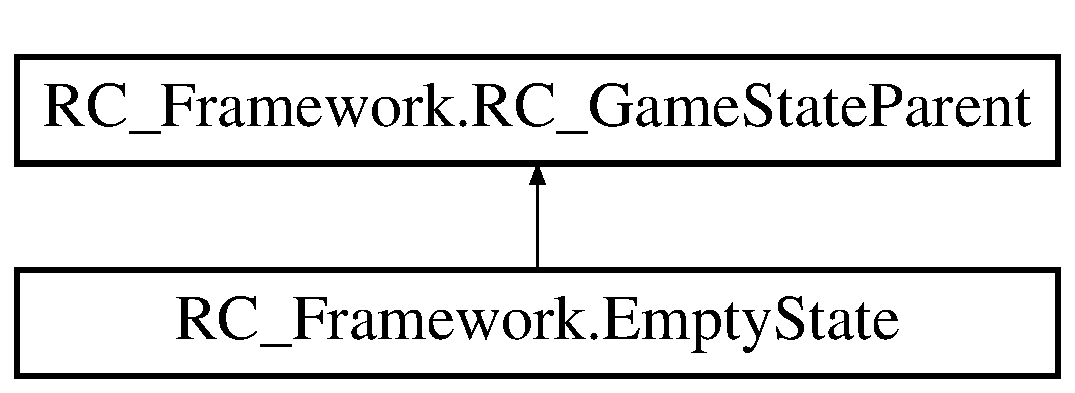
\includegraphics[height=2.000000cm]{class_r_c___framework_1_1_empty_state}
\end{center}
\end{figure}
\subsection*{Public Member Functions}
\begin{DoxyCompactItemize}
\item 
override void \mbox{\hyperlink{class_r_c___framework_1_1_empty_state_adfa60e364416dfe5f9a3ba565bc6329b}{Draw}} (Game\+Time game\+Time)
\end{DoxyCompactItemize}
\subsection*{Additional Inherited Members}


\subsection{Detailed Description}
A default \textquotesingle{}empty\textquotesingle{} level to fix probelms of having nothing to Draw or Update in short this class exists as a do nothing placeholder we need it in game initialisation and startup and it helps to simplify teaching 



\subsection{Member Function Documentation}
\mbox{\Hypertarget{class_r_c___framework_1_1_empty_state_adfa60e364416dfe5f9a3ba565bc6329b}\label{class_r_c___framework_1_1_empty_state_adfa60e364416dfe5f9a3ba565bc6329b}} 
\index{R\+C\+\_\+\+Framework\+::\+Empty\+State@{R\+C\+\_\+\+Framework\+::\+Empty\+State}!Draw@{Draw}}
\index{Draw@{Draw}!R\+C\+\_\+\+Framework\+::\+Empty\+State@{R\+C\+\_\+\+Framework\+::\+Empty\+State}}
\subsubsection{\texorpdfstring{Draw()}{Draw()}}
{\footnotesize\ttfamily override void R\+C\+\_\+\+Framework.\+Empty\+State.\+Draw (\begin{DoxyParamCaption}\item[{Game\+Time}]{game\+Time }\end{DoxyParamCaption})\hspace{0.3cm}{\ttfamily [virtual]}}



Implements \mbox{\hyperlink{class_r_c___framework_1_1_r_c___game_state_parent_adec421bc58a381ab34ffa74b495fa3c9}{R\+C\+\_\+\+Framework.\+R\+C\+\_\+\+Game\+State\+Parent}}.



The documentation for this class was generated from the following file\+:\begin{DoxyCompactItemize}
\item 
F\+:/\+B/\+R\+C\+\_\+\+Framework2018/\+Source/\mbox{\hyperlink{_r_c___game_state_8cs}{R\+C\+\_\+\+Game\+State.\+cs}}\end{DoxyCompactItemize}

\hypertarget{class_r_c___framework_1_1_font_parent}{}\section{R\+C\+\_\+\+Framework.\+Font\+Parent Class Reference}
\label{class_r_c___framework_1_1_font_parent}\index{R\+C\+\_\+\+Framework.\+Font\+Parent@{R\+C\+\_\+\+Framework.\+Font\+Parent}}


Parent class for all the bitmapped fonts stored in code  


Inheritance diagram for R\+C\+\_\+\+Framework.\+Font\+Parent\+:\begin{figure}[H]
\begin{center}
\leavevmode
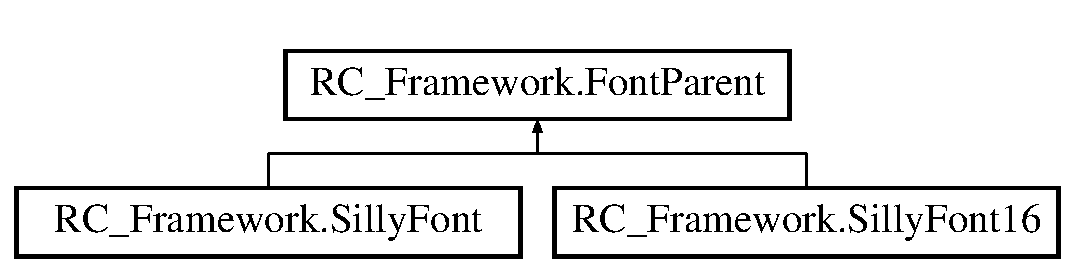
\includegraphics[height=2.000000cm]{class_r_c___framework_1_1_font_parent}
\end{center}
\end{figure}
\subsection*{Public Member Functions}
\begin{DoxyCompactItemize}
\item 
virtual int \mbox{\hyperlink{class_r_c___framework_1_1_font_parent_af32d5427b8feea59eb6f303ac3c36516}{charwidth}} ()
\item 
void \mbox{\hyperlink{class_r_c___framework_1_1_font_parent_a28b42b3aa17c44feb6f49065384ce9a7}{draw\+Char}} (Sprite\+Batch sb, Vector2 pos, char c, Color col)
\begin{DoxyCompactList}\small\item\em Draw a character at a given location in its default size \end{DoxyCompactList}\item 
void \mbox{\hyperlink{class_r_c___framework_1_1_font_parent_a8fb5fb02b85bc29031c0ccb8be1a7f61}{draw\+Char}} (Sprite\+Batch sb, Rectangle dest, char c, Color col)
\begin{DoxyCompactList}\small\item\em draw a character in a bounding rectangle \end{DoxyCompactList}\item 
void \mbox{\hyperlink{class_r_c___framework_1_1_font_parent_aa6d149fd5047fcc7b56dcbdcea21b5cc}{draw\+Str}} (Sprite\+Batch sb, Vector2 pos, string ss, Color col)
\begin{DoxyCompactList}\small\item\em draw a complete string at a given location \end{DoxyCompactList}\item 
void \mbox{\hyperlink{class_r_c___framework_1_1_font_parent_a4908cf6c8b915b517659eb1d1bef5a21}{draw\+Str}} (Sprite\+Batch sb, Vector2 pos, string ss, Color col, float char\+Width, float char\+Height)
\begin{DoxyCompactList}\small\item\em draw a string with specified character width and height \end{DoxyCompactList}\item 
void \mbox{\hyperlink{class_r_c___framework_1_1_font_parent_a54618265337f31d80bc6c82487855222}{draw\+Str\+Shadow}} (Sprite\+Batch sb, Vector2 pos, string ss, Color col, Color shadow\+Col, float char\+Width, float char\+Height, int x\+Offset, int y\+Offset)
\begin{DoxyCompactList}\small\item\em Draw the string twice with two diferent colours and a small offset to create a shadow effect \end{DoxyCompactList}\item 
void \mbox{\hyperlink{class_r_c___framework_1_1_font_parent_a4579edb7593917664d9d9d323a29cbae}{draw\+Str}} (Sprite\+Batch sb, Rectangle dest, string s, Color col)
\item 
void \mbox{\hyperlink{class_r_c___framework_1_1_font_parent_a8a6df4d62966f52f689d5a9738325797}{draw\+String}} (Sprite\+Batch sb, string text, Vector2 pos, Color col)
\begin{DoxyCompactList}\small\item\em To replace Sprite\+Batch.\+Draw\+String but with similar syntax always 12x12 aproximating 12 point font \end{DoxyCompactList}\end{DoxyCompactItemize}
\subsection*{Public Attributes}
\begin{DoxyCompactItemize}
\item 
Texture2D \mbox{[}$\,$\mbox{]} \mbox{\hyperlink{class_r_c___framework_1_1_font_parent_aa4656447cdf3ab637f839e814cdadaea}{fnt\+Tex}} = null
\item 
int \mbox{\hyperlink{class_r_c___framework_1_1_font_parent_a86ed779120a31be51fe4a70a29e50ef4}{char\+Set\+Size}} = 96
\item 
int \mbox{\hyperlink{class_r_c___framework_1_1_font_parent_acb860508d110915f5146e2554d115818}{char\+Set\+Size\+Extra}} = 1
\end{DoxyCompactItemize}


\subsection{Detailed Description}
Parent class for all the bitmapped fonts stored in code 



\subsection{Member Function Documentation}
\mbox{\Hypertarget{class_r_c___framework_1_1_font_parent_af32d5427b8feea59eb6f303ac3c36516}\label{class_r_c___framework_1_1_font_parent_af32d5427b8feea59eb6f303ac3c36516}} 
\index{R\+C\+\_\+\+Framework\+::\+Font\+Parent@{R\+C\+\_\+\+Framework\+::\+Font\+Parent}!charwidth@{charwidth}}
\index{charwidth@{charwidth}!R\+C\+\_\+\+Framework\+::\+Font\+Parent@{R\+C\+\_\+\+Framework\+::\+Font\+Parent}}
\subsubsection{\texorpdfstring{charwidth()}{charwidth()}}
{\footnotesize\ttfamily virtual int R\+C\+\_\+\+Framework.\+Font\+Parent.\+charwidth (\begin{DoxyParamCaption}{ }\end{DoxyParamCaption})\hspace{0.3cm}{\ttfamily [virtual]}}



Reimplemented in \mbox{\hyperlink{class_r_c___framework_1_1_silly_font16_aa718495839a1492ebf5d7245d7d4620a}{R\+C\+\_\+\+Framework.\+Silly\+Font16}}.

\mbox{\Hypertarget{class_r_c___framework_1_1_font_parent_a28b42b3aa17c44feb6f49065384ce9a7}\label{class_r_c___framework_1_1_font_parent_a28b42b3aa17c44feb6f49065384ce9a7}} 
\index{R\+C\+\_\+\+Framework\+::\+Font\+Parent@{R\+C\+\_\+\+Framework\+::\+Font\+Parent}!draw\+Char@{draw\+Char}}
\index{draw\+Char@{draw\+Char}!R\+C\+\_\+\+Framework\+::\+Font\+Parent@{R\+C\+\_\+\+Framework\+::\+Font\+Parent}}
\subsubsection{\texorpdfstring{draw\+Char()}{drawChar()}\hspace{0.1cm}{\footnotesize\ttfamily [1/2]}}
{\footnotesize\ttfamily void R\+C\+\_\+\+Framework.\+Font\+Parent.\+draw\+Char (\begin{DoxyParamCaption}\item[{Sprite\+Batch}]{sb,  }\item[{Vector2}]{pos,  }\item[{char}]{c,  }\item[{Color}]{col }\end{DoxyParamCaption})}



Draw a character at a given location in its default size 


\begin{DoxyParams}{Parameters}
{\em sb} & \\
\hline
{\em pos} & \\
\hline
{\em c} & \\
\hline
{\em col} & \\
\hline
\end{DoxyParams}
\mbox{\Hypertarget{class_r_c___framework_1_1_font_parent_a8fb5fb02b85bc29031c0ccb8be1a7f61}\label{class_r_c___framework_1_1_font_parent_a8fb5fb02b85bc29031c0ccb8be1a7f61}} 
\index{R\+C\+\_\+\+Framework\+::\+Font\+Parent@{R\+C\+\_\+\+Framework\+::\+Font\+Parent}!draw\+Char@{draw\+Char}}
\index{draw\+Char@{draw\+Char}!R\+C\+\_\+\+Framework\+::\+Font\+Parent@{R\+C\+\_\+\+Framework\+::\+Font\+Parent}}
\subsubsection{\texorpdfstring{draw\+Char()}{drawChar()}\hspace{0.1cm}{\footnotesize\ttfamily [2/2]}}
{\footnotesize\ttfamily void R\+C\+\_\+\+Framework.\+Font\+Parent.\+draw\+Char (\begin{DoxyParamCaption}\item[{Sprite\+Batch}]{sb,  }\item[{Rectangle}]{dest,  }\item[{char}]{c,  }\item[{Color}]{col }\end{DoxyParamCaption})}



draw a character in a bounding rectangle 


\begin{DoxyParams}{Parameters}
{\em sb} & \\
\hline
{\em dest} & \\
\hline
{\em c} & \\
\hline
{\em col} & \\
\hline
\end{DoxyParams}
\mbox{\Hypertarget{class_r_c___framework_1_1_font_parent_aa6d149fd5047fcc7b56dcbdcea21b5cc}\label{class_r_c___framework_1_1_font_parent_aa6d149fd5047fcc7b56dcbdcea21b5cc}} 
\index{R\+C\+\_\+\+Framework\+::\+Font\+Parent@{R\+C\+\_\+\+Framework\+::\+Font\+Parent}!draw\+Str@{draw\+Str}}
\index{draw\+Str@{draw\+Str}!R\+C\+\_\+\+Framework\+::\+Font\+Parent@{R\+C\+\_\+\+Framework\+::\+Font\+Parent}}
\subsubsection{\texorpdfstring{draw\+Str()}{drawStr()}\hspace{0.1cm}{\footnotesize\ttfamily [1/3]}}
{\footnotesize\ttfamily void R\+C\+\_\+\+Framework.\+Font\+Parent.\+draw\+Str (\begin{DoxyParamCaption}\item[{Sprite\+Batch}]{sb,  }\item[{Vector2}]{pos,  }\item[{string}]{ss,  }\item[{Color}]{col }\end{DoxyParamCaption})}



draw a complete string at a given location 


\begin{DoxyParams}{Parameters}
{\em sb} & \\
\hline
{\em pos} & \\
\hline
{\em ss} & \\
\hline
{\em col} & \\
\hline
\end{DoxyParams}
\mbox{\Hypertarget{class_r_c___framework_1_1_font_parent_a4908cf6c8b915b517659eb1d1bef5a21}\label{class_r_c___framework_1_1_font_parent_a4908cf6c8b915b517659eb1d1bef5a21}} 
\index{R\+C\+\_\+\+Framework\+::\+Font\+Parent@{R\+C\+\_\+\+Framework\+::\+Font\+Parent}!draw\+Str@{draw\+Str}}
\index{draw\+Str@{draw\+Str}!R\+C\+\_\+\+Framework\+::\+Font\+Parent@{R\+C\+\_\+\+Framework\+::\+Font\+Parent}}
\subsubsection{\texorpdfstring{draw\+Str()}{drawStr()}\hspace{0.1cm}{\footnotesize\ttfamily [2/3]}}
{\footnotesize\ttfamily void R\+C\+\_\+\+Framework.\+Font\+Parent.\+draw\+Str (\begin{DoxyParamCaption}\item[{Sprite\+Batch}]{sb,  }\item[{Vector2}]{pos,  }\item[{string}]{ss,  }\item[{Color}]{col,  }\item[{float}]{char\+Width,  }\item[{float}]{char\+Height }\end{DoxyParamCaption})}



draw a string with specified character width and height 


\begin{DoxyParams}{Parameters}
{\em sb} & \\
\hline
{\em pos} & \\
\hline
{\em ss} & \\
\hline
{\em col} & \\
\hline
{\em char\+Width} & \\
\hline
{\em char\+Height} & \\
\hline
\end{DoxyParams}
\mbox{\Hypertarget{class_r_c___framework_1_1_font_parent_a4579edb7593917664d9d9d323a29cbae}\label{class_r_c___framework_1_1_font_parent_a4579edb7593917664d9d9d323a29cbae}} 
\index{R\+C\+\_\+\+Framework\+::\+Font\+Parent@{R\+C\+\_\+\+Framework\+::\+Font\+Parent}!draw\+Str@{draw\+Str}}
\index{draw\+Str@{draw\+Str}!R\+C\+\_\+\+Framework\+::\+Font\+Parent@{R\+C\+\_\+\+Framework\+::\+Font\+Parent}}
\subsubsection{\texorpdfstring{draw\+Str()}{drawStr()}\hspace{0.1cm}{\footnotesize\ttfamily [3/3]}}
{\footnotesize\ttfamily void R\+C\+\_\+\+Framework.\+Font\+Parent.\+draw\+Str (\begin{DoxyParamCaption}\item[{Sprite\+Batch}]{sb,  }\item[{Rectangle}]{dest,  }\item[{string}]{s,  }\item[{Color}]{col }\end{DoxyParamCaption})}





draw a complete string in a bounding rectangle 


\begin{DoxyParams}{Parameters}
{\em sb} & \\
\hline
{\em dest} & \\
\hline
{\em s} & \\
\hline
{\em col} & \\
\hline
\end{DoxyParams}
\mbox{\Hypertarget{class_r_c___framework_1_1_font_parent_a8a6df4d62966f52f689d5a9738325797}\label{class_r_c___framework_1_1_font_parent_a8a6df4d62966f52f689d5a9738325797}} 
\index{R\+C\+\_\+\+Framework\+::\+Font\+Parent@{R\+C\+\_\+\+Framework\+::\+Font\+Parent}!draw\+String@{draw\+String}}
\index{draw\+String@{draw\+String}!R\+C\+\_\+\+Framework\+::\+Font\+Parent@{R\+C\+\_\+\+Framework\+::\+Font\+Parent}}
\subsubsection{\texorpdfstring{draw\+String()}{drawString()}}
{\footnotesize\ttfamily void R\+C\+\_\+\+Framework.\+Font\+Parent.\+draw\+String (\begin{DoxyParamCaption}\item[{Sprite\+Batch}]{sb,  }\item[{string}]{text,  }\item[{Vector2}]{pos,  }\item[{Color}]{col }\end{DoxyParamCaption})}



To replace Sprite\+Batch.\+Draw\+String but with similar syntax always 12x12 aproximating 12 point font 


\begin{DoxyParams}{Parameters}
{\em sb} & \\
\hline
{\em text} & \\
\hline
{\em pos} & \\
\hline
{\em col} & \\
\hline
\end{DoxyParams}
\mbox{\Hypertarget{class_r_c___framework_1_1_font_parent_a54618265337f31d80bc6c82487855222}\label{class_r_c___framework_1_1_font_parent_a54618265337f31d80bc6c82487855222}} 
\index{R\+C\+\_\+\+Framework\+::\+Font\+Parent@{R\+C\+\_\+\+Framework\+::\+Font\+Parent}!draw\+Str\+Shadow@{draw\+Str\+Shadow}}
\index{draw\+Str\+Shadow@{draw\+Str\+Shadow}!R\+C\+\_\+\+Framework\+::\+Font\+Parent@{R\+C\+\_\+\+Framework\+::\+Font\+Parent}}
\subsubsection{\texorpdfstring{draw\+Str\+Shadow()}{drawStrShadow()}}
{\footnotesize\ttfamily void R\+C\+\_\+\+Framework.\+Font\+Parent.\+draw\+Str\+Shadow (\begin{DoxyParamCaption}\item[{Sprite\+Batch}]{sb,  }\item[{Vector2}]{pos,  }\item[{string}]{ss,  }\item[{Color}]{col,  }\item[{Color}]{shadow\+Col,  }\item[{float}]{char\+Width,  }\item[{float}]{char\+Height,  }\item[{int}]{x\+Offset,  }\item[{int}]{y\+Offset }\end{DoxyParamCaption})}



Draw the string twice with two diferent colours and a small offset to create a shadow effect 


\begin{DoxyParams}{Parameters}
{\em sb} & \\
\hline
{\em pos} & \\
\hline
{\em ss} & \\
\hline
{\em col} & \\
\hline
{\em shadow\+Col} & \\
\hline
{\em char\+Width} & \\
\hline
{\em char\+Height} & \\
\hline
{\em x\+Offset} & \\
\hline
{\em y\+Offset} & \\
\hline
\end{DoxyParams}


\subsection{Member Data Documentation}
\mbox{\Hypertarget{class_r_c___framework_1_1_font_parent_a86ed779120a31be51fe4a70a29e50ef4}\label{class_r_c___framework_1_1_font_parent_a86ed779120a31be51fe4a70a29e50ef4}} 
\index{R\+C\+\_\+\+Framework\+::\+Font\+Parent@{R\+C\+\_\+\+Framework\+::\+Font\+Parent}!char\+Set\+Size@{char\+Set\+Size}}
\index{char\+Set\+Size@{char\+Set\+Size}!R\+C\+\_\+\+Framework\+::\+Font\+Parent@{R\+C\+\_\+\+Framework\+::\+Font\+Parent}}
\subsubsection{\texorpdfstring{char\+Set\+Size}{charSetSize}}
{\footnotesize\ttfamily int R\+C\+\_\+\+Framework.\+Font\+Parent.\+char\+Set\+Size = 96}

\mbox{\Hypertarget{class_r_c___framework_1_1_font_parent_acb860508d110915f5146e2554d115818}\label{class_r_c___framework_1_1_font_parent_acb860508d110915f5146e2554d115818}} 
\index{R\+C\+\_\+\+Framework\+::\+Font\+Parent@{R\+C\+\_\+\+Framework\+::\+Font\+Parent}!char\+Set\+Size\+Extra@{char\+Set\+Size\+Extra}}
\index{char\+Set\+Size\+Extra@{char\+Set\+Size\+Extra}!R\+C\+\_\+\+Framework\+::\+Font\+Parent@{R\+C\+\_\+\+Framework\+::\+Font\+Parent}}
\subsubsection{\texorpdfstring{char\+Set\+Size\+Extra}{charSetSizeExtra}}
{\footnotesize\ttfamily int R\+C\+\_\+\+Framework.\+Font\+Parent.\+char\+Set\+Size\+Extra = 1}

\mbox{\Hypertarget{class_r_c___framework_1_1_font_parent_aa4656447cdf3ab637f839e814cdadaea}\label{class_r_c___framework_1_1_font_parent_aa4656447cdf3ab637f839e814cdadaea}} 
\index{R\+C\+\_\+\+Framework\+::\+Font\+Parent@{R\+C\+\_\+\+Framework\+::\+Font\+Parent}!fnt\+Tex@{fnt\+Tex}}
\index{fnt\+Tex@{fnt\+Tex}!R\+C\+\_\+\+Framework\+::\+Font\+Parent@{R\+C\+\_\+\+Framework\+::\+Font\+Parent}}
\subsubsection{\texorpdfstring{fnt\+Tex}{fntTex}}
{\footnotesize\ttfamily Texture2D \mbox{[}$\,$\mbox{]} R\+C\+\_\+\+Framework.\+Font\+Parent.\+fnt\+Tex = null}



The documentation for this class was generated from the following file\+:\begin{DoxyCompactItemize}
\item 
F\+:/\+B/\+R\+C\+\_\+\+Framework2018/\+Source/\mbox{\hyperlink{_r_c___util_text_8cs}{R\+C\+\_\+\+Util\+Text.\+cs}}\end{DoxyCompactItemize}

\hypertarget{class_r_c___framework_1_1_frame}{}\section{R\+C\+\_\+\+Framework.\+Frame Class Reference}
\label{class_r_c___framework_1_1_frame}\index{R\+C\+\_\+\+Framework.\+Frame@{R\+C\+\_\+\+Framework.\+Frame}}


Simple Gui class with 1 image its usually a container for other classes  


Inheritance diagram for R\+C\+\_\+\+Framework.\+Frame\+:\begin{figure}[H]
\begin{center}
\leavevmode
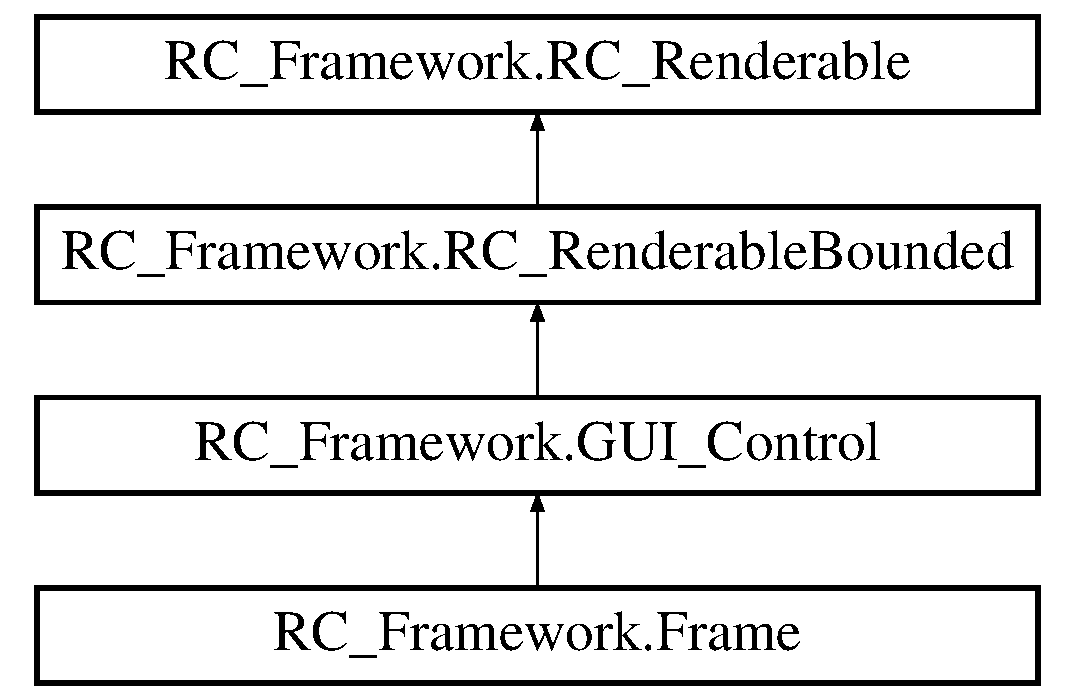
\includegraphics[height=4.000000cm]{class_r_c___framework_1_1_frame}
\end{center}
\end{figure}
\subsection*{Public Member Functions}
\begin{DoxyCompactItemize}
\item 
\mbox{\hyperlink{class_r_c___framework_1_1_frame_a9003d73a746ddb0cc3d0588830efb22d}{Frame}} (Texture2D t, Rectangle pos)
\begin{DoxyCompactList}\small\item\em default constructor \end{DoxyCompactList}\item 
override void \mbox{\hyperlink{class_r_c___framework_1_1_frame_ac27d7d9f33b34045c4dc90287f3eacee}{Draw}} (Sprite\+Batch sb)
\begin{DoxyCompactList}\small\item\em standard Draw \end{DoxyCompactList}\end{DoxyCompactItemize}
\subsection*{Additional Inherited Members}


\subsection{Detailed Description}
Simple Gui class with 1 image its usually a container for other classes 



\subsection{Constructor \& Destructor Documentation}
\mbox{\Hypertarget{class_r_c___framework_1_1_frame_a9003d73a746ddb0cc3d0588830efb22d}\label{class_r_c___framework_1_1_frame_a9003d73a746ddb0cc3d0588830efb22d}} 
\index{R\+C\+\_\+\+Framework\+::\+Frame@{R\+C\+\_\+\+Framework\+::\+Frame}!Frame@{Frame}}
\index{Frame@{Frame}!R\+C\+\_\+\+Framework\+::\+Frame@{R\+C\+\_\+\+Framework\+::\+Frame}}
\subsubsection{\texorpdfstring{Frame()}{Frame()}}
{\footnotesize\ttfamily R\+C\+\_\+\+Framework.\+Frame.\+Frame (\begin{DoxyParamCaption}\item[{Texture2D}]{t,  }\item[{Rectangle}]{pos }\end{DoxyParamCaption})}



default constructor 


\begin{DoxyParams}{Parameters}
{\em t} & \\
\hline
{\em pos} & \\
\hline
\end{DoxyParams}


\subsection{Member Function Documentation}
\mbox{\Hypertarget{class_r_c___framework_1_1_frame_ac27d7d9f33b34045c4dc90287f3eacee}\label{class_r_c___framework_1_1_frame_ac27d7d9f33b34045c4dc90287f3eacee}} 
\index{R\+C\+\_\+\+Framework\+::\+Frame@{R\+C\+\_\+\+Framework\+::\+Frame}!Draw@{Draw}}
\index{Draw@{Draw}!R\+C\+\_\+\+Framework\+::\+Frame@{R\+C\+\_\+\+Framework\+::\+Frame}}
\subsubsection{\texorpdfstring{Draw()}{Draw()}}
{\footnotesize\ttfamily override void R\+C\+\_\+\+Framework.\+Frame.\+Draw (\begin{DoxyParamCaption}\item[{Sprite\+Batch}]{sb }\end{DoxyParamCaption})\hspace{0.3cm}{\ttfamily [virtual]}}



standard Draw 


\begin{DoxyParams}{Parameters}
{\em sb} & \\
\hline
\end{DoxyParams}


Reimplemented from \mbox{\hyperlink{class_r_c___framework_1_1_r_c___renderable_acc26db34e382a25a989c4c0dd0354b23}{R\+C\+\_\+\+Framework.\+R\+C\+\_\+\+Renderable}}.



The documentation for this class was generated from the following file\+:\begin{DoxyCompactItemize}
\item 
F\+:/\+B/\+R\+C\+\_\+\+Framework2018/\+Source/\mbox{\hyperlink{_r_c___g_u_i_8cs}{R\+C\+\_\+\+G\+U\+I.\+cs}}\end{DoxyCompactItemize}

\hypertarget{class_r_c___framework_1_1_frame_list}{}\section{R\+C\+\_\+\+Framework.\+Frame\+List Class Reference}
\label{class_r_c___framework_1_1_frame_list}\index{R\+C\+\_\+\+Framework.\+Frame\+List@{R\+C\+\_\+\+Framework.\+Frame\+List}}
Inheritance diagram for R\+C\+\_\+\+Framework.\+Frame\+List\+:\begin{figure}[H]
\begin{center}
\leavevmode
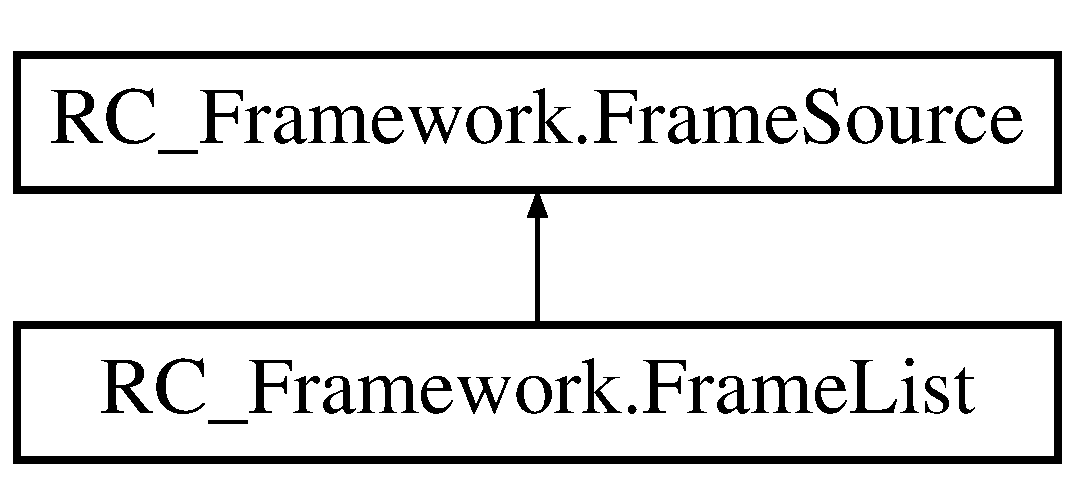
\includegraphics[height=2.000000cm]{class_r_c___framework_1_1_frame_list}
\end{center}
\end{figure}
\subsection*{Public Member Functions}
\begin{DoxyCompactItemize}
\item 
\mbox{\hyperlink{class_r_c___framework_1_1_frame_list_a1c3c1a8575092c34e47a77fc90100d71}{Frame\+List}} ()
\item 
void \mbox{\hyperlink{class_r_c___framework_1_1_frame_list_a0143dca563006dc8f6c6256cc69a0da2}{add\+To\+End}} (\mbox{\hyperlink{class_r_c___framework_1_1_r_c___frame}{R\+C\+\_\+\+Frame}} f)
\begin{DoxyCompactList}\small\item\em Adds a frame to the list \end{DoxyCompactList}\item 
override \mbox{\hyperlink{class_r_c___framework_1_1_r_c___frame}{R\+C\+\_\+\+Frame}} \mbox{\hyperlink{class_r_c___framework_1_1_frame_list_a5bfd1878eccd7e9e0c66f6e848383e6b}{get\+Frame}} (int num)
\begin{DoxyCompactList}\small\item\em return a specific frame based on number \end{DoxyCompactList}\item 
override \mbox{\hyperlink{class_r_c___framework_1_1_r_c___frame}{R\+C\+\_\+\+Frame}} \mbox{\hyperlink{class_r_c___framework_1_1_frame_list_ab91faad4e97b6e118d1b49d267d15b34}{get\+Frame}} ()
\begin{DoxyCompactList}\small\item\em Just a usefull default behaviour so everything compiles will generally not get used \end{DoxyCompactList}\item 
bool \mbox{\hyperlink{class_r_c___framework_1_1_frame_list_a298e87d53528b497f85fdf61bf519972}{set\+Frame}} (int num, \mbox{\hyperlink{class_r_c___framework_1_1_r_c___frame}{R\+C\+\_\+\+Frame}} f)
\item 
int \mbox{\hyperlink{class_r_c___framework_1_1_frame_list_a305c5e5f7911a8f066d1cc9f355541c3}{Count}} ()
\end{DoxyCompactItemize}
\subsection*{Public Attributes}
\begin{DoxyCompactItemize}
\item 
List$<$ \mbox{\hyperlink{class_r_c___framework_1_1_r_c___frame}{R\+C\+\_\+\+Frame}} $>$ \mbox{\hyperlink{class_r_c___framework_1_1_frame_list_ac79fd51ab4e22a0ac36da0020bb1f148}{flist}}
\end{DoxyCompactItemize}
\subsection*{Properties}
\begin{DoxyCompactItemize}
\item 
\mbox{\hyperlink{class_r_c___framework_1_1_r_c___frame}{R\+C\+\_\+\+Frame}} \mbox{\hyperlink{class_r_c___framework_1_1_frame_list_a7a404a856cc51b13a0ccecbeb07a66be}{this\mbox{[}int key\mbox{]}}}\hspace{0.3cm}{\ttfamily  \mbox{[}get, set\mbox{]}}
\begin{DoxyCompactList}\small\item\em Overload \mbox{[} and \mbox{]} for ease of use \end{DoxyCompactList}\end{DoxyCompactItemize}


\subsection{Constructor \& Destructor Documentation}
\mbox{\Hypertarget{class_r_c___framework_1_1_frame_list_a1c3c1a8575092c34e47a77fc90100d71}\label{class_r_c___framework_1_1_frame_list_a1c3c1a8575092c34e47a77fc90100d71}} 
\index{R\+C\+\_\+\+Framework\+::\+Frame\+List@{R\+C\+\_\+\+Framework\+::\+Frame\+List}!Frame\+List@{Frame\+List}}
\index{Frame\+List@{Frame\+List}!R\+C\+\_\+\+Framework\+::\+Frame\+List@{R\+C\+\_\+\+Framework\+::\+Frame\+List}}
\subsubsection{\texorpdfstring{Frame\+List()}{FrameList()}}
{\footnotesize\ttfamily R\+C\+\_\+\+Framework.\+Frame\+List.\+Frame\+List (\begin{DoxyParamCaption}{ }\end{DoxyParamCaption})}



\subsection{Member Function Documentation}
\mbox{\Hypertarget{class_r_c___framework_1_1_frame_list_a0143dca563006dc8f6c6256cc69a0da2}\label{class_r_c___framework_1_1_frame_list_a0143dca563006dc8f6c6256cc69a0da2}} 
\index{R\+C\+\_\+\+Framework\+::\+Frame\+List@{R\+C\+\_\+\+Framework\+::\+Frame\+List}!add\+To\+End@{add\+To\+End}}
\index{add\+To\+End@{add\+To\+End}!R\+C\+\_\+\+Framework\+::\+Frame\+List@{R\+C\+\_\+\+Framework\+::\+Frame\+List}}
\subsubsection{\texorpdfstring{add\+To\+End()}{addToEnd()}}
{\footnotesize\ttfamily void R\+C\+\_\+\+Framework.\+Frame\+List.\+add\+To\+End (\begin{DoxyParamCaption}\item[{\mbox{\hyperlink{class_r_c___framework_1_1_r_c___frame}{R\+C\+\_\+\+Frame}}}]{f }\end{DoxyParamCaption})}



Adds a frame to the list 


\begin{DoxyParams}{Parameters}
{\em r} & \\
\hline
\end{DoxyParams}
\mbox{\Hypertarget{class_r_c___framework_1_1_frame_list_a305c5e5f7911a8f066d1cc9f355541c3}\label{class_r_c___framework_1_1_frame_list_a305c5e5f7911a8f066d1cc9f355541c3}} 
\index{R\+C\+\_\+\+Framework\+::\+Frame\+List@{R\+C\+\_\+\+Framework\+::\+Frame\+List}!Count@{Count}}
\index{Count@{Count}!R\+C\+\_\+\+Framework\+::\+Frame\+List@{R\+C\+\_\+\+Framework\+::\+Frame\+List}}
\subsubsection{\texorpdfstring{Count()}{Count()}}
{\footnotesize\ttfamily int R\+C\+\_\+\+Framework.\+Frame\+List.\+Count (\begin{DoxyParamCaption}{ }\end{DoxyParamCaption})}

\mbox{\Hypertarget{class_r_c___framework_1_1_frame_list_a5bfd1878eccd7e9e0c66f6e848383e6b}\label{class_r_c___framework_1_1_frame_list_a5bfd1878eccd7e9e0c66f6e848383e6b}} 
\index{R\+C\+\_\+\+Framework\+::\+Frame\+List@{R\+C\+\_\+\+Framework\+::\+Frame\+List}!get\+Frame@{get\+Frame}}
\index{get\+Frame@{get\+Frame}!R\+C\+\_\+\+Framework\+::\+Frame\+List@{R\+C\+\_\+\+Framework\+::\+Frame\+List}}
\subsubsection{\texorpdfstring{get\+Frame()}{getFrame()}\hspace{0.1cm}{\footnotesize\ttfamily [1/2]}}
{\footnotesize\ttfamily override \mbox{\hyperlink{class_r_c___framework_1_1_r_c___frame}{R\+C\+\_\+\+Frame}} R\+C\+\_\+\+Framework.\+Frame\+List.\+get\+Frame (\begin{DoxyParamCaption}\item[{int}]{num }\end{DoxyParamCaption})\hspace{0.3cm}{\ttfamily [virtual]}}



return a specific frame based on number 


\begin{DoxyParams}{Parameters}
{\em num} & \\
\hline
\end{DoxyParams}
\begin{DoxyReturn}{Returns}

\end{DoxyReturn}


Implements \mbox{\hyperlink{class_r_c___framework_1_1_frame_source_a562dc295b5c265ec760227978802eb3a}{R\+C\+\_\+\+Framework.\+Frame\+Source}}.

\mbox{\Hypertarget{class_r_c___framework_1_1_frame_list_ab91faad4e97b6e118d1b49d267d15b34}\label{class_r_c___framework_1_1_frame_list_ab91faad4e97b6e118d1b49d267d15b34}} 
\index{R\+C\+\_\+\+Framework\+::\+Frame\+List@{R\+C\+\_\+\+Framework\+::\+Frame\+List}!get\+Frame@{get\+Frame}}
\index{get\+Frame@{get\+Frame}!R\+C\+\_\+\+Framework\+::\+Frame\+List@{R\+C\+\_\+\+Framework\+::\+Frame\+List}}
\subsubsection{\texorpdfstring{get\+Frame()}{getFrame()}\hspace{0.1cm}{\footnotesize\ttfamily [2/2]}}
{\footnotesize\ttfamily override \mbox{\hyperlink{class_r_c___framework_1_1_r_c___frame}{R\+C\+\_\+\+Frame}} R\+C\+\_\+\+Framework.\+Frame\+List.\+get\+Frame (\begin{DoxyParamCaption}{ }\end{DoxyParamCaption})\hspace{0.3cm}{\ttfamily [virtual]}}



Just a usefull default behaviour so everything compiles will generally not get used 

\begin{DoxyReturn}{Returns}

\end{DoxyReturn}


Implements \mbox{\hyperlink{class_r_c___framework_1_1_frame_source_a6fd84a8d608da7d9ff2ff5ab10ed4243}{R\+C\+\_\+\+Framework.\+Frame\+Source}}.

\mbox{\Hypertarget{class_r_c___framework_1_1_frame_list_a298e87d53528b497f85fdf61bf519972}\label{class_r_c___framework_1_1_frame_list_a298e87d53528b497f85fdf61bf519972}} 
\index{R\+C\+\_\+\+Framework\+::\+Frame\+List@{R\+C\+\_\+\+Framework\+::\+Frame\+List}!set\+Frame@{set\+Frame}}
\index{set\+Frame@{set\+Frame}!R\+C\+\_\+\+Framework\+::\+Frame\+List@{R\+C\+\_\+\+Framework\+::\+Frame\+List}}
\subsubsection{\texorpdfstring{set\+Frame()}{setFrame()}}
{\footnotesize\ttfamily bool R\+C\+\_\+\+Framework.\+Frame\+List.\+set\+Frame (\begin{DoxyParamCaption}\item[{int}]{num,  }\item[{\mbox{\hyperlink{class_r_c___framework_1_1_r_c___frame}{R\+C\+\_\+\+Frame}}}]{f }\end{DoxyParamCaption})}



\subsection{Member Data Documentation}
\mbox{\Hypertarget{class_r_c___framework_1_1_frame_list_ac79fd51ab4e22a0ac36da0020bb1f148}\label{class_r_c___framework_1_1_frame_list_ac79fd51ab4e22a0ac36da0020bb1f148}} 
\index{R\+C\+\_\+\+Framework\+::\+Frame\+List@{R\+C\+\_\+\+Framework\+::\+Frame\+List}!flist@{flist}}
\index{flist@{flist}!R\+C\+\_\+\+Framework\+::\+Frame\+List@{R\+C\+\_\+\+Framework\+::\+Frame\+List}}
\subsubsection{\texorpdfstring{flist}{flist}}
{\footnotesize\ttfamily List$<$\mbox{\hyperlink{class_r_c___framework_1_1_r_c___frame}{R\+C\+\_\+\+Frame}}$>$ R\+C\+\_\+\+Framework.\+Frame\+List.\+flist}



\subsection{Property Documentation}
\mbox{\Hypertarget{class_r_c___framework_1_1_frame_list_a7a404a856cc51b13a0ccecbeb07a66be}\label{class_r_c___framework_1_1_frame_list_a7a404a856cc51b13a0ccecbeb07a66be}} 
\index{R\+C\+\_\+\+Framework\+::\+Frame\+List@{R\+C\+\_\+\+Framework\+::\+Frame\+List}!this\mbox{[}int key\mbox{]}@{this[int key]}}
\index{this\mbox{[}int key\mbox{]}@{this[int key]}!R\+C\+\_\+\+Framework\+::\+Frame\+List@{R\+C\+\_\+\+Framework\+::\+Frame\+List}}
\subsubsection{\texorpdfstring{this[int key]}{this[int key]}}
{\footnotesize\ttfamily \mbox{\hyperlink{class_r_c___framework_1_1_r_c___frame}{R\+C\+\_\+\+Frame}} R\+C\+\_\+\+Framework.\+Frame\+List.\+this\mbox{[}int key\mbox{]}\hspace{0.3cm}{\ttfamily [get]}, {\ttfamily [set]}}



Overload \mbox{[} and \mbox{]} for ease of use 


\begin{DoxyParams}{Parameters}
{\em key} & \\
\hline
\end{DoxyParams}
\begin{DoxyReturn}{Returns}

\end{DoxyReturn}


The documentation for this class was generated from the following file\+:\begin{DoxyCompactItemize}
\item 
F\+:/\+B/\+R\+C\+\_\+\+Framework2018/\+Source/\mbox{\hyperlink{_r_c___frame_8cs}{R\+C\+\_\+\+Frame.\+cs}}\end{DoxyCompactItemize}

\hypertarget{class_r_c___framework_1_1_frame_source}{}\section{R\+C\+\_\+\+Framework.\+Frame\+Source Class Reference}
\label{class_r_c___framework_1_1_frame_source}\index{R\+C\+\_\+\+Framework.\+Frame\+Source@{R\+C\+\_\+\+Framework.\+Frame\+Source}}


Abstract class to get a numbered frame  


Inheritance diagram for R\+C\+\_\+\+Framework.\+Frame\+Source\+:\begin{figure}[H]
\begin{center}
\leavevmode
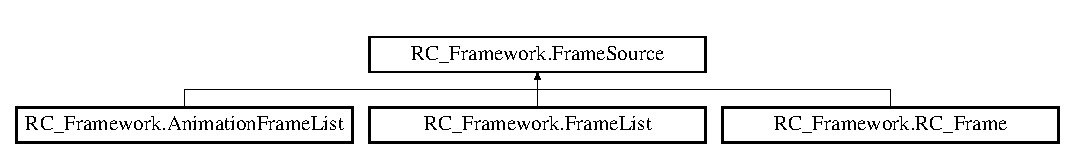
\includegraphics[height=1.689291cm]{class_r_c___framework_1_1_frame_source}
\end{center}
\end{figure}
\subsection*{Public Member Functions}
\begin{DoxyCompactItemize}
\item 
abstract \mbox{\hyperlink{class_r_c___framework_1_1_r_c___frame}{R\+C\+\_\+\+Frame}} \mbox{\hyperlink{class_r_c___framework_1_1_frame_source_a6fd84a8d608da7d9ff2ff5ab10ed4243}{get\+Frame}} ()
\begin{DoxyCompactList}\small\item\em this one method must be overridden and return the current frame or null \end{DoxyCompactList}\item 
abstract \mbox{\hyperlink{class_r_c___framework_1_1_r_c___frame}{R\+C\+\_\+\+Frame}} \mbox{\hyperlink{class_r_c___framework_1_1_frame_source_a562dc295b5c265ec760227978802eb3a}{get\+Frame}} (int num)
\begin{DoxyCompactList}\small\item\em this method is usually overridden and returns a numbered frame for any given number (or null) \end{DoxyCompactList}\item 
virtual void \mbox{\hyperlink{class_r_c___framework_1_1_frame_source_a4ab94513c0555c16316b540aed1e9144}{Update}} (Game\+Time game\+Time)
\begin{DoxyCompactList}\small\item\em Update so the frames can advance if necessary \end{DoxyCompactList}\end{DoxyCompactItemize}


\subsection{Detailed Description}
Abstract class to get a numbered frame 



\subsection{Member Function Documentation}
\mbox{\Hypertarget{class_r_c___framework_1_1_frame_source_a6fd84a8d608da7d9ff2ff5ab10ed4243}\label{class_r_c___framework_1_1_frame_source_a6fd84a8d608da7d9ff2ff5ab10ed4243}} 
\index{R\+C\+\_\+\+Framework\+::\+Frame\+Source@{R\+C\+\_\+\+Framework\+::\+Frame\+Source}!get\+Frame@{get\+Frame}}
\index{get\+Frame@{get\+Frame}!R\+C\+\_\+\+Framework\+::\+Frame\+Source@{R\+C\+\_\+\+Framework\+::\+Frame\+Source}}
\subsubsection{\texorpdfstring{get\+Frame()}{getFrame()}\hspace{0.1cm}{\footnotesize\ttfamily [1/2]}}
{\footnotesize\ttfamily abstract \mbox{\hyperlink{class_r_c___framework_1_1_r_c___frame}{R\+C\+\_\+\+Frame}} R\+C\+\_\+\+Framework.\+Frame\+Source.\+get\+Frame (\begin{DoxyParamCaption}{ }\end{DoxyParamCaption})\hspace{0.3cm}{\ttfamily [pure virtual]}}



this one method must be overridden and return the current frame or null 


\begin{DoxyParams}{Parameters}
{\em num} & \\
\hline
\end{DoxyParams}
\begin{DoxyReturn}{Returns}

\end{DoxyReturn}


Implemented in \mbox{\hyperlink{class_r_c___framework_1_1_animation_frame_list_a5bc162ddb15e2ef4f98b72be2720a87b}{R\+C\+\_\+\+Framework.\+Animation\+Frame\+List}}, \mbox{\hyperlink{class_r_c___framework_1_1_frame_list_ab91faad4e97b6e118d1b49d267d15b34}{R\+C\+\_\+\+Framework.\+Frame\+List}}, and \mbox{\hyperlink{class_r_c___framework_1_1_r_c___frame_a9262ade99ade9dc102aac56587d55d0f}{R\+C\+\_\+\+Framework.\+R\+C\+\_\+\+Frame}}.

\mbox{\Hypertarget{class_r_c___framework_1_1_frame_source_a562dc295b5c265ec760227978802eb3a}\label{class_r_c___framework_1_1_frame_source_a562dc295b5c265ec760227978802eb3a}} 
\index{R\+C\+\_\+\+Framework\+::\+Frame\+Source@{R\+C\+\_\+\+Framework\+::\+Frame\+Source}!get\+Frame@{get\+Frame}}
\index{get\+Frame@{get\+Frame}!R\+C\+\_\+\+Framework\+::\+Frame\+Source@{R\+C\+\_\+\+Framework\+::\+Frame\+Source}}
\subsubsection{\texorpdfstring{get\+Frame()}{getFrame()}\hspace{0.1cm}{\footnotesize\ttfamily [2/2]}}
{\footnotesize\ttfamily abstract \mbox{\hyperlink{class_r_c___framework_1_1_r_c___frame}{R\+C\+\_\+\+Frame}} R\+C\+\_\+\+Framework.\+Frame\+Source.\+get\+Frame (\begin{DoxyParamCaption}\item[{int}]{num }\end{DoxyParamCaption})\hspace{0.3cm}{\ttfamily [pure virtual]}}



this method is usually overridden and returns a numbered frame for any given number (or null) 


\begin{DoxyParams}{Parameters}
{\em num} & \\
\hline
\end{DoxyParams}
\begin{DoxyReturn}{Returns}

\end{DoxyReturn}


Implemented in \mbox{\hyperlink{class_r_c___framework_1_1_animation_frame_list_aa253565464d98bf955c81702fd3d66a4}{R\+C\+\_\+\+Framework.\+Animation\+Frame\+List}}, \mbox{\hyperlink{class_r_c___framework_1_1_frame_list_a5bfd1878eccd7e9e0c66f6e848383e6b}{R\+C\+\_\+\+Framework.\+Frame\+List}}, and \mbox{\hyperlink{class_r_c___framework_1_1_r_c___frame_ad0a2ae1e80157a79713552d9484eb5de}{R\+C\+\_\+\+Framework.\+R\+C\+\_\+\+Frame}}.

\mbox{\Hypertarget{class_r_c___framework_1_1_frame_source_a4ab94513c0555c16316b540aed1e9144}\label{class_r_c___framework_1_1_frame_source_a4ab94513c0555c16316b540aed1e9144}} 
\index{R\+C\+\_\+\+Framework\+::\+Frame\+Source@{R\+C\+\_\+\+Framework\+::\+Frame\+Source}!Update@{Update}}
\index{Update@{Update}!R\+C\+\_\+\+Framework\+::\+Frame\+Source@{R\+C\+\_\+\+Framework\+::\+Frame\+Source}}
\subsubsection{\texorpdfstring{Update()}{Update()}}
{\footnotesize\ttfamily virtual void R\+C\+\_\+\+Framework.\+Frame\+Source.\+Update (\begin{DoxyParamCaption}\item[{Game\+Time}]{game\+Time }\end{DoxyParamCaption})\hspace{0.3cm}{\ttfamily [virtual]}}



Update so the frames can advance if necessary 


\begin{DoxyParams}{Parameters}
{\em game\+Time} & \\
\hline
\end{DoxyParams}


Reimplemented in \mbox{\hyperlink{class_r_c___framework_1_1_animation_frame_list_ad6d3b045da01a972a32f48ae7b7c7598}{R\+C\+\_\+\+Framework.\+Animation\+Frame\+List}}.



The documentation for this class was generated from the following file\+:\begin{DoxyCompactItemize}
\item 
F\+:/\+B/\+R\+C\+\_\+\+Framework2018/\+Source/\mbox{\hyperlink{_r_c___frame_8cs}{R\+C\+\_\+\+Frame.\+cs}}\end{DoxyCompactItemize}

\hypertarget{class_r_c___framework_1_1_grid_back_ground}{}\section{R\+C\+\_\+\+Framework.\+Grid\+Back\+Ground Class Reference}
\label{class_r_c___framework_1_1_grid_back_ground}\index{R\+C\+\_\+\+Framework.\+Grid\+Back\+Ground@{R\+C\+\_\+\+Framework.\+Grid\+Back\+Ground}}


Draws a grid in a rectangle It can be acurately positioned by changing Offset It can be animated by changing delta and update\+Modulo Vertoical or horizontal lines may be omitted by setting draw\+Vertical or draw\+Horizontal to false  


Inheritance diagram for R\+C\+\_\+\+Framework.\+Grid\+Back\+Ground\+:\begin{figure}[H]
\begin{center}
\leavevmode
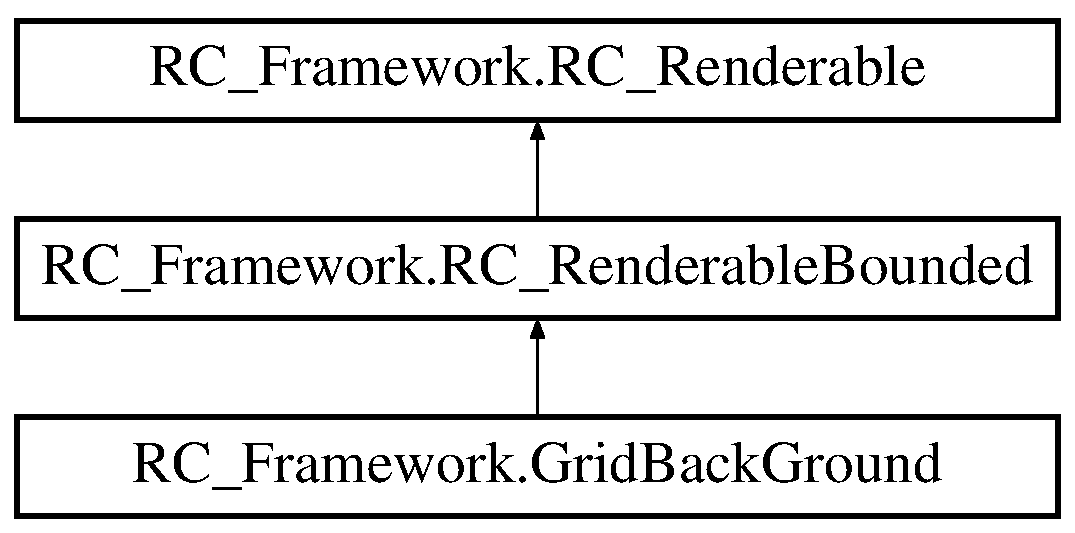
\includegraphics[height=3.000000cm]{class_r_c___framework_1_1_grid_back_ground}
\end{center}
\end{figure}
\subsection*{Public Member Functions}
\begin{DoxyCompactItemize}
\item 
\mbox{\hyperlink{class_r_c___framework_1_1_grid_back_ground_ac58b15afcc3b7fddc9aaa0f8decd3d7c}{Grid\+Back\+Ground}} (Rectangle boundZ, Color line\+Color, Color back\+Color, Vector2 spacing, int line\+WidthZ)
\item 
override void \mbox{\hyperlink{class_r_c___framework_1_1_grid_back_ground_a242904271618f793025f4dfae9681c13}{Draw}} (Sprite\+Batch sb)
\begin{DoxyCompactList}\small\item\em Standard draw routine which assumes the renderable knows where it is \end{DoxyCompactList}\item 
override void \mbox{\hyperlink{class_r_c___framework_1_1_grid_back_ground_af43061e6a0067ad6c3043b6ddb080de4}{Update}} (Game\+Time game\+Time)
\item 
override void \mbox{\hyperlink{class_r_c___framework_1_1_grid_back_ground_aeaa4759b7da2f73fd760f0e9d59aa97c}{reset}} ()
\end{DoxyCompactItemize}
\subsection*{Public Attributes}
\begin{DoxyCompactItemize}
\item 
Color \mbox{\hyperlink{class_r_c___framework_1_1_grid_back_ground_aea6b48adc0f7198e7e174272e27a38fc}{line\+Colour2}} = Color.\+Black
\item 
int \mbox{\hyperlink{class_r_c___framework_1_1_grid_back_ground_a70bd87e07cf3c796c46bfabbf5deb484}{ticks\+To\+Lerp}} = 1
\item 
Vector2 \mbox{\hyperlink{class_r_c___framework_1_1_grid_back_ground_a218136f423b8aa4b2bf9294628f3a9b7}{offset}}
\item 
Vector2 \mbox{\hyperlink{class_r_c___framework_1_1_grid_back_ground_a52aae8ab0c66a1ba7a83874828742c81}{delta}}
\item 
bool \mbox{\hyperlink{class_r_c___framework_1_1_grid_back_ground_a72db0e3bc139d962dd84d918f3f443b7}{draw\+Background}} = true
\item 
int \mbox{\hyperlink{class_r_c___framework_1_1_grid_back_ground_a3995a8339610de394109a7d00c91cf12}{update\+Modulo}} =1
\item 
bool \mbox{\hyperlink{class_r_c___framework_1_1_grid_back_ground_ad2dcba9e3bd46129cc3066fe7a4fafe4}{draw\+Vertical}} = true
\item 
bool \mbox{\hyperlink{class_r_c___framework_1_1_grid_back_ground_aaa1851c8b283367cc1d79bdb8c27ce32}{draw\+Horizontal}} = true
\end{DoxyCompactItemize}
\subsection*{Additional Inherited Members}


\subsection{Detailed Description}
Draws a grid in a rectangle It can be acurately positioned by changing Offset It can be animated by changing delta and update\+Modulo Vertoical or horizontal lines may be omitted by setting draw\+Vertical or draw\+Horizontal to false 

Ticks to lerp and linecolour2 can be set to change the grid colour so it sort of pulsates colour example setup may be\+: r9b = new \mbox{\hyperlink{class_r_c___framework_1_1_grid_back_ground}{Grid\+Back\+Ground}}(new Rectangle(10, 300, 200, 200), Color.\+Red, Color.\+Blanched\+Almond, new Vector2(30, 20), 2); r9b.\+delta = new Vector2(1, 0); // speed of animation r9b.\+update\+Modulo = 2; // try 30 to slow it a bit

or\+: ~\newline
\begin{DoxyVerb}  r9c = new GridBackGround(new Rectangle(260, 10, 200, 200), Color.Red, Color.Silver, new Vector2(30, 20), 2);
  r9c.delta = new Vector2(0f,0.2f); // speed of animation
  r9c.updateModulo = 2; // try 30 to slow it a bit
  r9c.ticksToLerp = 120;
  r9c.lineColour2 = new Color(255, 255, 255);
\end{DoxyVerb}
 

\subsection{Constructor \& Destructor Documentation}
\mbox{\Hypertarget{class_r_c___framework_1_1_grid_back_ground_ac58b15afcc3b7fddc9aaa0f8decd3d7c}\label{class_r_c___framework_1_1_grid_back_ground_ac58b15afcc3b7fddc9aaa0f8decd3d7c}} 
\index{R\+C\+\_\+\+Framework\+::\+Grid\+Back\+Ground@{R\+C\+\_\+\+Framework\+::\+Grid\+Back\+Ground}!Grid\+Back\+Ground@{Grid\+Back\+Ground}}
\index{Grid\+Back\+Ground@{Grid\+Back\+Ground}!R\+C\+\_\+\+Framework\+::\+Grid\+Back\+Ground@{R\+C\+\_\+\+Framework\+::\+Grid\+Back\+Ground}}
\subsubsection{\texorpdfstring{Grid\+Back\+Ground()}{GridBackGround()}}
{\footnotesize\ttfamily R\+C\+\_\+\+Framework.\+Grid\+Back\+Ground.\+Grid\+Back\+Ground (\begin{DoxyParamCaption}\item[{Rectangle}]{boundZ,  }\item[{Color}]{line\+Color,  }\item[{Color}]{back\+Color,  }\item[{Vector2}]{spacing,  }\item[{int}]{line\+WidthZ }\end{DoxyParamCaption})}



\subsection{Member Function Documentation}
\mbox{\Hypertarget{class_r_c___framework_1_1_grid_back_ground_a242904271618f793025f4dfae9681c13}\label{class_r_c___framework_1_1_grid_back_ground_a242904271618f793025f4dfae9681c13}} 
\index{R\+C\+\_\+\+Framework\+::\+Grid\+Back\+Ground@{R\+C\+\_\+\+Framework\+::\+Grid\+Back\+Ground}!Draw@{Draw}}
\index{Draw@{Draw}!R\+C\+\_\+\+Framework\+::\+Grid\+Back\+Ground@{R\+C\+\_\+\+Framework\+::\+Grid\+Back\+Ground}}
\subsubsection{\texorpdfstring{Draw()}{Draw()}}
{\footnotesize\ttfamily override void R\+C\+\_\+\+Framework.\+Grid\+Back\+Ground.\+Draw (\begin{DoxyParamCaption}\item[{Sprite\+Batch}]{sb }\end{DoxyParamCaption})\hspace{0.3cm}{\ttfamily [virtual]}}



Standard draw routine which assumes the renderable knows where it is 


\begin{DoxyParams}{Parameters}
{\em sb} & \\
\hline
\end{DoxyParams}


Reimplemented from \mbox{\hyperlink{class_r_c___framework_1_1_r_c___renderable_acc26db34e382a25a989c4c0dd0354b23}{R\+C\+\_\+\+Framework.\+R\+C\+\_\+\+Renderable}}.

\mbox{\Hypertarget{class_r_c___framework_1_1_grid_back_ground_aeaa4759b7da2f73fd760f0e9d59aa97c}\label{class_r_c___framework_1_1_grid_back_ground_aeaa4759b7da2f73fd760f0e9d59aa97c}} 
\index{R\+C\+\_\+\+Framework\+::\+Grid\+Back\+Ground@{R\+C\+\_\+\+Framework\+::\+Grid\+Back\+Ground}!reset@{reset}}
\index{reset@{reset}!R\+C\+\_\+\+Framework\+::\+Grid\+Back\+Ground@{R\+C\+\_\+\+Framework\+::\+Grid\+Back\+Ground}}
\subsubsection{\texorpdfstring{reset()}{reset()}}
{\footnotesize\ttfamily override void R\+C\+\_\+\+Framework.\+Grid\+Back\+Ground.\+reset (\begin{DoxyParamCaption}{ }\end{DoxyParamCaption})\hspace{0.3cm}{\ttfamily [virtual]}}



Reimplemented from \mbox{\hyperlink{class_r_c___framework_1_1_r_c___renderable_ae65ce69704d15963789f421b58618b1f}{R\+C\+\_\+\+Framework.\+R\+C\+\_\+\+Renderable}}.

\mbox{\Hypertarget{class_r_c___framework_1_1_grid_back_ground_af43061e6a0067ad6c3043b6ddb080de4}\label{class_r_c___framework_1_1_grid_back_ground_af43061e6a0067ad6c3043b6ddb080de4}} 
\index{R\+C\+\_\+\+Framework\+::\+Grid\+Back\+Ground@{R\+C\+\_\+\+Framework\+::\+Grid\+Back\+Ground}!Update@{Update}}
\index{Update@{Update}!R\+C\+\_\+\+Framework\+::\+Grid\+Back\+Ground@{R\+C\+\_\+\+Framework\+::\+Grid\+Back\+Ground}}
\subsubsection{\texorpdfstring{Update()}{Update()}}
{\footnotesize\ttfamily override void R\+C\+\_\+\+Framework.\+Grid\+Back\+Ground.\+Update (\begin{DoxyParamCaption}\item[{Game\+Time}]{game\+Time }\end{DoxyParamCaption})\hspace{0.3cm}{\ttfamily [virtual]}}



Reimplemented from \mbox{\hyperlink{class_r_c___framework_1_1_r_c___renderable_a5745bedc7ba0587aa1e1d8563c357228}{R\+C\+\_\+\+Framework.\+R\+C\+\_\+\+Renderable}}.



\subsection{Member Data Documentation}
\mbox{\Hypertarget{class_r_c___framework_1_1_grid_back_ground_a52aae8ab0c66a1ba7a83874828742c81}\label{class_r_c___framework_1_1_grid_back_ground_a52aae8ab0c66a1ba7a83874828742c81}} 
\index{R\+C\+\_\+\+Framework\+::\+Grid\+Back\+Ground@{R\+C\+\_\+\+Framework\+::\+Grid\+Back\+Ground}!delta@{delta}}
\index{delta@{delta}!R\+C\+\_\+\+Framework\+::\+Grid\+Back\+Ground@{R\+C\+\_\+\+Framework\+::\+Grid\+Back\+Ground}}
\subsubsection{\texorpdfstring{delta}{delta}}
{\footnotesize\ttfamily Vector2 R\+C\+\_\+\+Framework.\+Grid\+Back\+Ground.\+delta}

\mbox{\Hypertarget{class_r_c___framework_1_1_grid_back_ground_a72db0e3bc139d962dd84d918f3f443b7}\label{class_r_c___framework_1_1_grid_back_ground_a72db0e3bc139d962dd84d918f3f443b7}} 
\index{R\+C\+\_\+\+Framework\+::\+Grid\+Back\+Ground@{R\+C\+\_\+\+Framework\+::\+Grid\+Back\+Ground}!draw\+Background@{draw\+Background}}
\index{draw\+Background@{draw\+Background}!R\+C\+\_\+\+Framework\+::\+Grid\+Back\+Ground@{R\+C\+\_\+\+Framework\+::\+Grid\+Back\+Ground}}
\subsubsection{\texorpdfstring{draw\+Background}{drawBackground}}
{\footnotesize\ttfamily bool R\+C\+\_\+\+Framework.\+Grid\+Back\+Ground.\+draw\+Background = true}

\mbox{\Hypertarget{class_r_c___framework_1_1_grid_back_ground_aaa1851c8b283367cc1d79bdb8c27ce32}\label{class_r_c___framework_1_1_grid_back_ground_aaa1851c8b283367cc1d79bdb8c27ce32}} 
\index{R\+C\+\_\+\+Framework\+::\+Grid\+Back\+Ground@{R\+C\+\_\+\+Framework\+::\+Grid\+Back\+Ground}!draw\+Horizontal@{draw\+Horizontal}}
\index{draw\+Horizontal@{draw\+Horizontal}!R\+C\+\_\+\+Framework\+::\+Grid\+Back\+Ground@{R\+C\+\_\+\+Framework\+::\+Grid\+Back\+Ground}}
\subsubsection{\texorpdfstring{draw\+Horizontal}{drawHorizontal}}
{\footnotesize\ttfamily bool R\+C\+\_\+\+Framework.\+Grid\+Back\+Ground.\+draw\+Horizontal = true}

\mbox{\Hypertarget{class_r_c___framework_1_1_grid_back_ground_ad2dcba9e3bd46129cc3066fe7a4fafe4}\label{class_r_c___framework_1_1_grid_back_ground_ad2dcba9e3bd46129cc3066fe7a4fafe4}} 
\index{R\+C\+\_\+\+Framework\+::\+Grid\+Back\+Ground@{R\+C\+\_\+\+Framework\+::\+Grid\+Back\+Ground}!draw\+Vertical@{draw\+Vertical}}
\index{draw\+Vertical@{draw\+Vertical}!R\+C\+\_\+\+Framework\+::\+Grid\+Back\+Ground@{R\+C\+\_\+\+Framework\+::\+Grid\+Back\+Ground}}
\subsubsection{\texorpdfstring{draw\+Vertical}{drawVertical}}
{\footnotesize\ttfamily bool R\+C\+\_\+\+Framework.\+Grid\+Back\+Ground.\+draw\+Vertical = true}

\mbox{\Hypertarget{class_r_c___framework_1_1_grid_back_ground_aea6b48adc0f7198e7e174272e27a38fc}\label{class_r_c___framework_1_1_grid_back_ground_aea6b48adc0f7198e7e174272e27a38fc}} 
\index{R\+C\+\_\+\+Framework\+::\+Grid\+Back\+Ground@{R\+C\+\_\+\+Framework\+::\+Grid\+Back\+Ground}!line\+Colour2@{line\+Colour2}}
\index{line\+Colour2@{line\+Colour2}!R\+C\+\_\+\+Framework\+::\+Grid\+Back\+Ground@{R\+C\+\_\+\+Framework\+::\+Grid\+Back\+Ground}}
\subsubsection{\texorpdfstring{line\+Colour2}{lineColour2}}
{\footnotesize\ttfamily Color R\+C\+\_\+\+Framework.\+Grid\+Back\+Ground.\+line\+Colour2 = Color.\+Black}

\mbox{\Hypertarget{class_r_c___framework_1_1_grid_back_ground_a218136f423b8aa4b2bf9294628f3a9b7}\label{class_r_c___framework_1_1_grid_back_ground_a218136f423b8aa4b2bf9294628f3a9b7}} 
\index{R\+C\+\_\+\+Framework\+::\+Grid\+Back\+Ground@{R\+C\+\_\+\+Framework\+::\+Grid\+Back\+Ground}!offset@{offset}}
\index{offset@{offset}!R\+C\+\_\+\+Framework\+::\+Grid\+Back\+Ground@{R\+C\+\_\+\+Framework\+::\+Grid\+Back\+Ground}}
\subsubsection{\texorpdfstring{offset}{offset}}
{\footnotesize\ttfamily Vector2 R\+C\+\_\+\+Framework.\+Grid\+Back\+Ground.\+offset}

\mbox{\Hypertarget{class_r_c___framework_1_1_grid_back_ground_a70bd87e07cf3c796c46bfabbf5deb484}\label{class_r_c___framework_1_1_grid_back_ground_a70bd87e07cf3c796c46bfabbf5deb484}} 
\index{R\+C\+\_\+\+Framework\+::\+Grid\+Back\+Ground@{R\+C\+\_\+\+Framework\+::\+Grid\+Back\+Ground}!ticks\+To\+Lerp@{ticks\+To\+Lerp}}
\index{ticks\+To\+Lerp@{ticks\+To\+Lerp}!R\+C\+\_\+\+Framework\+::\+Grid\+Back\+Ground@{R\+C\+\_\+\+Framework\+::\+Grid\+Back\+Ground}}
\subsubsection{\texorpdfstring{ticks\+To\+Lerp}{ticksToLerp}}
{\footnotesize\ttfamily int R\+C\+\_\+\+Framework.\+Grid\+Back\+Ground.\+ticks\+To\+Lerp = 1}

\mbox{\Hypertarget{class_r_c___framework_1_1_grid_back_ground_a3995a8339610de394109a7d00c91cf12}\label{class_r_c___framework_1_1_grid_back_ground_a3995a8339610de394109a7d00c91cf12}} 
\index{R\+C\+\_\+\+Framework\+::\+Grid\+Back\+Ground@{R\+C\+\_\+\+Framework\+::\+Grid\+Back\+Ground}!update\+Modulo@{update\+Modulo}}
\index{update\+Modulo@{update\+Modulo}!R\+C\+\_\+\+Framework\+::\+Grid\+Back\+Ground@{R\+C\+\_\+\+Framework\+::\+Grid\+Back\+Ground}}
\subsubsection{\texorpdfstring{update\+Modulo}{updateModulo}}
{\footnotesize\ttfamily int R\+C\+\_\+\+Framework.\+Grid\+Back\+Ground.\+update\+Modulo =1}



The documentation for this class was generated from the following file\+:\begin{DoxyCompactItemize}
\item 
F\+:/\+B/\+R\+C\+\_\+\+Framework2018/\+Source/\mbox{\hyperlink{_r_c___renderable_bounded_8cs}{R\+C\+\_\+\+Renderable\+Bounded.\+cs}}\end{DoxyCompactItemize}

\hypertarget{class_r_c___framework_1_1_g_u_i___control}{}\section{R\+C\+\_\+\+Framework.\+G\+U\+I\+\_\+\+Control Class Reference}
\label{class_r_c___framework_1_1_g_u_i___control}\index{R\+C\+\_\+\+Framework.\+G\+U\+I\+\_\+\+Control@{R\+C\+\_\+\+Framework.\+G\+U\+I\+\_\+\+Control}}


G\+UI parent class This is the parent class for all gui objects  


Inheritance diagram for R\+C\+\_\+\+Framework.\+G\+U\+I\+\_\+\+Control\+:\begin{figure}[H]
\begin{center}
\leavevmode
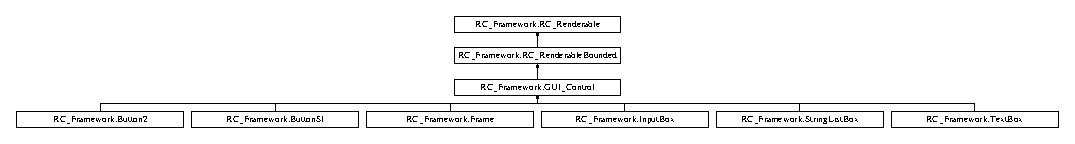
\includegraphics[height=1.493333cm]{class_r_c___framework_1_1_g_u_i___control}
\end{center}
\end{figure}
\subsection*{Public Member Functions}
\begin{DoxyCompactItemize}
\item 
override bool \mbox{\hyperlink{class_r_c___framework_1_1_g_u_i___control_a005e7f109afd21abd6576fdf70212af5}{Mouse\+Down\+Event\+Left}} (float mouse\+\_\+x, float mouse\+\_\+y)
\begin{DoxyCompactList}\small\item\em Handle left mouse click \end{DoxyCompactList}\item 
override bool \mbox{\hyperlink{class_r_c___framework_1_1_g_u_i___control_ad5f72ceb3149305ce0a2891feff951a0}{Mouse\+Over}} (float mouse\+\_\+x, float mouse\+\_\+y)
\begin{DoxyCompactList}\small\item\em handle mouse over event (eg tool tips) \end{DoxyCompactList}\item 
virtual void \mbox{\hyperlink{class_r_c___framework_1_1_g_u_i___control_a5e2a0dbd0e76b4753ee7e33c5873f099}{draw\+Sub\+Controls}} (Sprite\+Batch sb)
\begin{DoxyCompactList}\small\item\em draw my sub controls if any \end{DoxyCompactList}\item 
\mbox{\hyperlink{class_r_c___framework_1_1_g_u_i___control_aba58c5937d3c44703c5b4c7be4701a47}{G\+U\+I\+\_\+\+Control}} ()
\begin{DoxyCompactList}\small\item\em Default constructor \end{DoxyCompactList}\item 
void \mbox{\hyperlink{class_r_c___framework_1_1_g_u_i___control_ae53955f2d8f4a2be9dffbfabfe0901d7}{set\+Tool\+Tip}} (String \mbox{\hyperlink{class_r_c___framework_1_1_r_c___renderable_a255c5d9294a719e56855890f3535d129}{text}})
\begin{DoxyCompactList}\small\item\em Set the tool tip for this control \end{DoxyCompactList}\item 
void \mbox{\hyperlink{class_r_c___framework_1_1_g_u_i___control_a55f2748c142671a1e73a188204768f93}{Clear}} ()
\begin{DoxyCompactList}\small\item\em remove all sub controls \end{DoxyCompactList}\item 
void \mbox{\hyperlink{class_r_c___framework_1_1_g_u_i___control_a462903d09f92efd24da0bde3c689b3ef}{Add\+Control}} (\mbox{\hyperlink{class_r_c___framework_1_1_g_u_i___control}{G\+U\+I\+\_\+\+Control}} c)
\begin{DoxyCompactList}\small\item\em add a sub control making me its parent \end{DoxyCompactList}\item 
\mbox{\hyperlink{class_r_c___framework_1_1_g_u_i___control}{G\+U\+I\+\_\+\+Control}} \mbox{\hyperlink{class_r_c___framework_1_1_g_u_i___control_a2808c23510a4448a8928d4393eaa3751}{get\+Control}} (int cnum)
\begin{DoxyCompactList}\small\item\em get a control if you know its index \end{DoxyCompactList}\item 
Boolean \mbox{\hyperlink{class_r_c___framework_1_1_g_u_i___control_a810c7c0dfb643da1861b8e2627642aa1}{inside}} (float x, float y)
\begin{DoxyCompactList}\small\item\em Return a boolean that is true if the point is inside the bounds and the control is visible \end{DoxyCompactList}\item 
void \mbox{\hyperlink{class_r_c___framework_1_1_g_u_i___control_a31b8425ebb4e7f35ddae9736e98e8d5c}{clear\+Focus}} (bool clear\+Parent)
\begin{DoxyCompactList}\small\item\em clear focus on me and my sub controlls \end{DoxyCompactList}\item 
Vector2 \mbox{\hyperlink{class_r_c___framework_1_1_g_u_i___control_aec3a07f10f946dff6dd7563eff7a786d}{get\+Screen\+Pos}} ()
\begin{DoxyCompactList}\small\item\em Get my position on the actual screen as adjusted by my parents position \end{DoxyCompactList}\item 
override bool \mbox{\hyperlink{class_r_c___framework_1_1_g_u_i___control_a458eb00bda180db22ebe22e550a669a4}{Key\+Hit\+Event}} (Keys key\+Hit)
\begin{DoxyCompactList}\small\item\em key hit handling \end{DoxyCompactList}\item 
bool \mbox{\hyperlink{class_r_c___framework_1_1_g_u_i___control_a8e4abd4dc7a2243fc309fb80c984ef9e}{pass\+On\+Keyhit}} (Keys key\+Hit)
\begin{DoxyCompactList}\small\item\em Send the key hit to my sub controls \end{DoxyCompactList}\item 
override void \mbox{\hyperlink{class_r_c___framework_1_1_g_u_i___control_a7aa3b0b6ba141d995ca830ff99ae3003}{Update}} (Game\+Time game\+Time)
\begin{DoxyCompactList}\small\item\em Update \end{DoxyCompactList}\item 
void \mbox{\hyperlink{class_r_c___framework_1_1_g_u_i___control_a19b896ae0239a880458192de438e217c}{set\+Color}} (Color c, bool pass\+On)
\begin{DoxyCompactList}\small\item\em Set my colour and all my sub controlls colour usefull to control transparency \end{DoxyCompactList}\end{DoxyCompactItemize}
\subsection*{Public Attributes}
\begin{DoxyCompactItemize}
\item 
List$<$ \mbox{\hyperlink{class_r_c___framework_1_1_g_u_i___control}{G\+U\+I\+\_\+\+Control}} $>$ \mbox{\hyperlink{class_r_c___framework_1_1_g_u_i___control_a38f8a94f8ae576e42dbce0c043ee31fb}{controls}} = null
\begin{DoxyCompactList}\small\item\em Ny list of sub controls -\/ usually you dont need to touch this \end{DoxyCompactList}\item 
bool \mbox{\hyperlink{class_r_c___framework_1_1_g_u_i___control_a51a1c0b4ed5abd5322dd3975d28c9cec}{focus}} =false
\begin{DoxyCompactList}\small\item\em Do i have focus \end{DoxyCompactList}\item 
\mbox{\hyperlink{class_r_c___framework_1_1_g_u_i___control}{G\+U\+I\+\_\+\+Control}} \mbox{\hyperlink{class_r_c___framework_1_1_g_u_i___control_ac1d70b73574da322d588be9d890a5167}{parent}} =null
\begin{DoxyCompactList}\small\item\em My parent control or null \end{DoxyCompactList}\item 
String \mbox{\hyperlink{class_r_c___framework_1_1_g_u_i___control_a815044c81674b4e0f31124e9dc66978b}{t\+Ttext}} =\char`\"{}\char`\"{}
\begin{DoxyCompactList}\small\item\em tool tip text string \end{DoxyCompactList}\end{DoxyCompactItemize}
\subsection*{Additional Inherited Members}


\subsection{Detailed Description}
G\+UI parent class This is the parent class for all gui objects 



\subsection{Constructor \& Destructor Documentation}
\mbox{\Hypertarget{class_r_c___framework_1_1_g_u_i___control_aba58c5937d3c44703c5b4c7be4701a47}\label{class_r_c___framework_1_1_g_u_i___control_aba58c5937d3c44703c5b4c7be4701a47}} 
\index{R\+C\+\_\+\+Framework\+::\+G\+U\+I\+\_\+\+Control@{R\+C\+\_\+\+Framework\+::\+G\+U\+I\+\_\+\+Control}!G\+U\+I\+\_\+\+Control@{G\+U\+I\+\_\+\+Control}}
\index{G\+U\+I\+\_\+\+Control@{G\+U\+I\+\_\+\+Control}!R\+C\+\_\+\+Framework\+::\+G\+U\+I\+\_\+\+Control@{R\+C\+\_\+\+Framework\+::\+G\+U\+I\+\_\+\+Control}}
\subsubsection{\texorpdfstring{G\+U\+I\+\_\+\+Control()}{GUI\_Control()}}
{\footnotesize\ttfamily R\+C\+\_\+\+Framework.\+G\+U\+I\+\_\+\+Control.\+G\+U\+I\+\_\+\+Control (\begin{DoxyParamCaption}{ }\end{DoxyParamCaption})}



Default constructor 



\subsection{Member Function Documentation}
\mbox{\Hypertarget{class_r_c___framework_1_1_g_u_i___control_a462903d09f92efd24da0bde3c689b3ef}\label{class_r_c___framework_1_1_g_u_i___control_a462903d09f92efd24da0bde3c689b3ef}} 
\index{R\+C\+\_\+\+Framework\+::\+G\+U\+I\+\_\+\+Control@{R\+C\+\_\+\+Framework\+::\+G\+U\+I\+\_\+\+Control}!Add\+Control@{Add\+Control}}
\index{Add\+Control@{Add\+Control}!R\+C\+\_\+\+Framework\+::\+G\+U\+I\+\_\+\+Control@{R\+C\+\_\+\+Framework\+::\+G\+U\+I\+\_\+\+Control}}
\subsubsection{\texorpdfstring{Add\+Control()}{AddControl()}}
{\footnotesize\ttfamily void R\+C\+\_\+\+Framework.\+G\+U\+I\+\_\+\+Control.\+Add\+Control (\begin{DoxyParamCaption}\item[{\mbox{\hyperlink{class_r_c___framework_1_1_g_u_i___control}{G\+U\+I\+\_\+\+Control}}}]{c }\end{DoxyParamCaption})}



add a sub control making me its parent 


\begin{DoxyParams}{Parameters}
{\em c} & \\
\hline
\end{DoxyParams}
\mbox{\Hypertarget{class_r_c___framework_1_1_g_u_i___control_a55f2748c142671a1e73a188204768f93}\label{class_r_c___framework_1_1_g_u_i___control_a55f2748c142671a1e73a188204768f93}} 
\index{R\+C\+\_\+\+Framework\+::\+G\+U\+I\+\_\+\+Control@{R\+C\+\_\+\+Framework\+::\+G\+U\+I\+\_\+\+Control}!Clear@{Clear}}
\index{Clear@{Clear}!R\+C\+\_\+\+Framework\+::\+G\+U\+I\+\_\+\+Control@{R\+C\+\_\+\+Framework\+::\+G\+U\+I\+\_\+\+Control}}
\subsubsection{\texorpdfstring{Clear()}{Clear()}}
{\footnotesize\ttfamily void R\+C\+\_\+\+Framework.\+G\+U\+I\+\_\+\+Control.\+Clear (\begin{DoxyParamCaption}{ }\end{DoxyParamCaption})}



remove all sub controls 

\mbox{\Hypertarget{class_r_c___framework_1_1_g_u_i___control_a31b8425ebb4e7f35ddae9736e98e8d5c}\label{class_r_c___framework_1_1_g_u_i___control_a31b8425ebb4e7f35ddae9736e98e8d5c}} 
\index{R\+C\+\_\+\+Framework\+::\+G\+U\+I\+\_\+\+Control@{R\+C\+\_\+\+Framework\+::\+G\+U\+I\+\_\+\+Control}!clear\+Focus@{clear\+Focus}}
\index{clear\+Focus@{clear\+Focus}!R\+C\+\_\+\+Framework\+::\+G\+U\+I\+\_\+\+Control@{R\+C\+\_\+\+Framework\+::\+G\+U\+I\+\_\+\+Control}}
\subsubsection{\texorpdfstring{clear\+Focus()}{clearFocus()}}
{\footnotesize\ttfamily void R\+C\+\_\+\+Framework.\+G\+U\+I\+\_\+\+Control.\+clear\+Focus (\begin{DoxyParamCaption}\item[{bool}]{clear\+Parent }\end{DoxyParamCaption})}



clear focus on me and my sub controlls 


\begin{DoxyParams}{Parameters}
{\em clear\+Parent} & \\
\hline
\end{DoxyParams}
\mbox{\Hypertarget{class_r_c___framework_1_1_g_u_i___control_a5e2a0dbd0e76b4753ee7e33c5873f099}\label{class_r_c___framework_1_1_g_u_i___control_a5e2a0dbd0e76b4753ee7e33c5873f099}} 
\index{R\+C\+\_\+\+Framework\+::\+G\+U\+I\+\_\+\+Control@{R\+C\+\_\+\+Framework\+::\+G\+U\+I\+\_\+\+Control}!draw\+Sub\+Controls@{draw\+Sub\+Controls}}
\index{draw\+Sub\+Controls@{draw\+Sub\+Controls}!R\+C\+\_\+\+Framework\+::\+G\+U\+I\+\_\+\+Control@{R\+C\+\_\+\+Framework\+::\+G\+U\+I\+\_\+\+Control}}
\subsubsection{\texorpdfstring{draw\+Sub\+Controls()}{drawSubControls()}}
{\footnotesize\ttfamily virtual void R\+C\+\_\+\+Framework.\+G\+U\+I\+\_\+\+Control.\+draw\+Sub\+Controls (\begin{DoxyParamCaption}\item[{Sprite\+Batch}]{sb }\end{DoxyParamCaption})\hspace{0.3cm}{\ttfamily [virtual]}}



draw my sub controls if any 


\begin{DoxyParams}{Parameters}
{\em sb} & \\
\hline
\end{DoxyParams}
\mbox{\Hypertarget{class_r_c___framework_1_1_g_u_i___control_a2808c23510a4448a8928d4393eaa3751}\label{class_r_c___framework_1_1_g_u_i___control_a2808c23510a4448a8928d4393eaa3751}} 
\index{R\+C\+\_\+\+Framework\+::\+G\+U\+I\+\_\+\+Control@{R\+C\+\_\+\+Framework\+::\+G\+U\+I\+\_\+\+Control}!get\+Control@{get\+Control}}
\index{get\+Control@{get\+Control}!R\+C\+\_\+\+Framework\+::\+G\+U\+I\+\_\+\+Control@{R\+C\+\_\+\+Framework\+::\+G\+U\+I\+\_\+\+Control}}
\subsubsection{\texorpdfstring{get\+Control()}{getControl()}}
{\footnotesize\ttfamily \mbox{\hyperlink{class_r_c___framework_1_1_g_u_i___control}{G\+U\+I\+\_\+\+Control}} R\+C\+\_\+\+Framework.\+G\+U\+I\+\_\+\+Control.\+get\+Control (\begin{DoxyParamCaption}\item[{int}]{cnum }\end{DoxyParamCaption})}



get a control if you know its index 


\begin{DoxyParams}{Parameters}
{\em cnum} & \\
\hline
\end{DoxyParams}
\begin{DoxyReturn}{Returns}

\end{DoxyReturn}
\mbox{\Hypertarget{class_r_c___framework_1_1_g_u_i___control_aec3a07f10f946dff6dd7563eff7a786d}\label{class_r_c___framework_1_1_g_u_i___control_aec3a07f10f946dff6dd7563eff7a786d}} 
\index{R\+C\+\_\+\+Framework\+::\+G\+U\+I\+\_\+\+Control@{R\+C\+\_\+\+Framework\+::\+G\+U\+I\+\_\+\+Control}!get\+Screen\+Pos@{get\+Screen\+Pos}}
\index{get\+Screen\+Pos@{get\+Screen\+Pos}!R\+C\+\_\+\+Framework\+::\+G\+U\+I\+\_\+\+Control@{R\+C\+\_\+\+Framework\+::\+G\+U\+I\+\_\+\+Control}}
\subsubsection{\texorpdfstring{get\+Screen\+Pos()}{getScreenPos()}}
{\footnotesize\ttfamily Vector2 R\+C\+\_\+\+Framework.\+G\+U\+I\+\_\+\+Control.\+get\+Screen\+Pos (\begin{DoxyParamCaption}{ }\end{DoxyParamCaption})}



Get my position on the actual screen as adjusted by my parents position 

\begin{DoxyReturn}{Returns}

\end{DoxyReturn}
\mbox{\Hypertarget{class_r_c___framework_1_1_g_u_i___control_a810c7c0dfb643da1861b8e2627642aa1}\label{class_r_c___framework_1_1_g_u_i___control_a810c7c0dfb643da1861b8e2627642aa1}} 
\index{R\+C\+\_\+\+Framework\+::\+G\+U\+I\+\_\+\+Control@{R\+C\+\_\+\+Framework\+::\+G\+U\+I\+\_\+\+Control}!inside@{inside}}
\index{inside@{inside}!R\+C\+\_\+\+Framework\+::\+G\+U\+I\+\_\+\+Control@{R\+C\+\_\+\+Framework\+::\+G\+U\+I\+\_\+\+Control}}
\subsubsection{\texorpdfstring{inside()}{inside()}}
{\footnotesize\ttfamily Boolean R\+C\+\_\+\+Framework.\+G\+U\+I\+\_\+\+Control.\+inside (\begin{DoxyParamCaption}\item[{float}]{x,  }\item[{float}]{y }\end{DoxyParamCaption})}



Return a boolean that is true if the point is inside the bounds and the control is visible 

\mbox{\Hypertarget{class_r_c___framework_1_1_g_u_i___control_a458eb00bda180db22ebe22e550a669a4}\label{class_r_c___framework_1_1_g_u_i___control_a458eb00bda180db22ebe22e550a669a4}} 
\index{R\+C\+\_\+\+Framework\+::\+G\+U\+I\+\_\+\+Control@{R\+C\+\_\+\+Framework\+::\+G\+U\+I\+\_\+\+Control}!Key\+Hit\+Event@{Key\+Hit\+Event}}
\index{Key\+Hit\+Event@{Key\+Hit\+Event}!R\+C\+\_\+\+Framework\+::\+G\+U\+I\+\_\+\+Control@{R\+C\+\_\+\+Framework\+::\+G\+U\+I\+\_\+\+Control}}
\subsubsection{\texorpdfstring{Key\+Hit\+Event()}{KeyHitEvent()}}
{\footnotesize\ttfamily override bool R\+C\+\_\+\+Framework.\+G\+U\+I\+\_\+\+Control.\+Key\+Hit\+Event (\begin{DoxyParamCaption}\item[{Keys}]{key\+Hit }\end{DoxyParamCaption})\hspace{0.3cm}{\ttfamily [virtual]}}



key hit handling 


\begin{DoxyParams}{Parameters}
{\em key\+Hit} & \\
\hline
\end{DoxyParams}
\begin{DoxyReturn}{Returns}

\end{DoxyReturn}


Reimplemented from \mbox{\hyperlink{class_r_c___framework_1_1_r_c___renderable_a826da9b07316c475186e4c2f00648827}{R\+C\+\_\+\+Framework.\+R\+C\+\_\+\+Renderable}}.



Reimplemented in \mbox{\hyperlink{class_r_c___framework_1_1_string_list_box_a8b449ef1c2c786786b7e6cf52f416750}{R\+C\+\_\+\+Framework.\+String\+List\+Box}}, \mbox{\hyperlink{class_r_c___framework_1_1_input_box_a07ef881a281e4da95994e54ec1f7b496}{R\+C\+\_\+\+Framework.\+Input\+Box}}, and \mbox{\hyperlink{class_r_c___framework_1_1_text_box_ae8c28e507b2c91aa042e2a5c2a300598}{R\+C\+\_\+\+Framework.\+Text\+Box}}.

\mbox{\Hypertarget{class_r_c___framework_1_1_g_u_i___control_a005e7f109afd21abd6576fdf70212af5}\label{class_r_c___framework_1_1_g_u_i___control_a005e7f109afd21abd6576fdf70212af5}} 
\index{R\+C\+\_\+\+Framework\+::\+G\+U\+I\+\_\+\+Control@{R\+C\+\_\+\+Framework\+::\+G\+U\+I\+\_\+\+Control}!Mouse\+Down\+Event\+Left@{Mouse\+Down\+Event\+Left}}
\index{Mouse\+Down\+Event\+Left@{Mouse\+Down\+Event\+Left}!R\+C\+\_\+\+Framework\+::\+G\+U\+I\+\_\+\+Control@{R\+C\+\_\+\+Framework\+::\+G\+U\+I\+\_\+\+Control}}
\subsubsection{\texorpdfstring{Mouse\+Down\+Event\+Left()}{MouseDownEventLeft()}}
{\footnotesize\ttfamily override bool R\+C\+\_\+\+Framework.\+G\+U\+I\+\_\+\+Control.\+Mouse\+Down\+Event\+Left (\begin{DoxyParamCaption}\item[{float}]{mouse\+\_\+x,  }\item[{float}]{mouse\+\_\+y }\end{DoxyParamCaption})\hspace{0.3cm}{\ttfamily [virtual]}}



Handle left mouse click 


\begin{DoxyParams}{Parameters}
{\em mouse\+\_\+x} & \\
\hline
{\em mouse\+\_\+y} & \\
\hline
\end{DoxyParams}
\begin{DoxyReturn}{Returns}

\end{DoxyReturn}


Reimplemented from \mbox{\hyperlink{class_r_c___framework_1_1_r_c___renderable_a41d144d6fad27f219d861e61a2d9796e}{R\+C\+\_\+\+Framework.\+R\+C\+\_\+\+Renderable}}.



Reimplemented in \mbox{\hyperlink{class_r_c___framework_1_1_string_list_box_aabe8c72a90d47c67eb162c76b1e7f79c}{R\+C\+\_\+\+Framework.\+String\+List\+Box}}, \mbox{\hyperlink{class_r_c___framework_1_1_input_box_a7e57c860483df9645d726d6adbbc6dab}{R\+C\+\_\+\+Framework.\+Input\+Box}}, \mbox{\hyperlink{class_r_c___framework_1_1_text_box_a73f9a94392ff9bf3639a37a29470fb63}{R\+C\+\_\+\+Framework.\+Text\+Box}}, \mbox{\hyperlink{class_r_c___framework_1_1_button_s_i_a4323f8436749655b240fa35caa15daa6}{R\+C\+\_\+\+Framework.\+Button\+SI}}, and \mbox{\hyperlink{class_r_c___framework_1_1_button2_ac15728fbc9e908a70990c159ecd5824f}{R\+C\+\_\+\+Framework.\+Button2}}.

\mbox{\Hypertarget{class_r_c___framework_1_1_g_u_i___control_ad5f72ceb3149305ce0a2891feff951a0}\label{class_r_c___framework_1_1_g_u_i___control_ad5f72ceb3149305ce0a2891feff951a0}} 
\index{R\+C\+\_\+\+Framework\+::\+G\+U\+I\+\_\+\+Control@{R\+C\+\_\+\+Framework\+::\+G\+U\+I\+\_\+\+Control}!Mouse\+Over@{Mouse\+Over}}
\index{Mouse\+Over@{Mouse\+Over}!R\+C\+\_\+\+Framework\+::\+G\+U\+I\+\_\+\+Control@{R\+C\+\_\+\+Framework\+::\+G\+U\+I\+\_\+\+Control}}
\subsubsection{\texorpdfstring{Mouse\+Over()}{MouseOver()}}
{\footnotesize\ttfamily override bool R\+C\+\_\+\+Framework.\+G\+U\+I\+\_\+\+Control.\+Mouse\+Over (\begin{DoxyParamCaption}\item[{float}]{mouse\+\_\+x,  }\item[{float}]{mouse\+\_\+y }\end{DoxyParamCaption})\hspace{0.3cm}{\ttfamily [virtual]}}



handle mouse over event (eg tool tips) 


\begin{DoxyParams}{Parameters}
{\em mouse\+\_\+x} & \\
\hline
{\em mouse\+\_\+y} & \\
\hline
\end{DoxyParams}
\begin{DoxyReturn}{Returns}

\end{DoxyReturn}


Reimplemented from \mbox{\hyperlink{class_r_c___framework_1_1_r_c___renderable_abd55ea96d88d7bd2207e3a4ede1f1a05}{R\+C\+\_\+\+Framework.\+R\+C\+\_\+\+Renderable}}.

\mbox{\Hypertarget{class_r_c___framework_1_1_g_u_i___control_a8e4abd4dc7a2243fc309fb80c984ef9e}\label{class_r_c___framework_1_1_g_u_i___control_a8e4abd4dc7a2243fc309fb80c984ef9e}} 
\index{R\+C\+\_\+\+Framework\+::\+G\+U\+I\+\_\+\+Control@{R\+C\+\_\+\+Framework\+::\+G\+U\+I\+\_\+\+Control}!pass\+On\+Keyhit@{pass\+On\+Keyhit}}
\index{pass\+On\+Keyhit@{pass\+On\+Keyhit}!R\+C\+\_\+\+Framework\+::\+G\+U\+I\+\_\+\+Control@{R\+C\+\_\+\+Framework\+::\+G\+U\+I\+\_\+\+Control}}
\subsubsection{\texorpdfstring{pass\+On\+Keyhit()}{passOnKeyhit()}}
{\footnotesize\ttfamily bool R\+C\+\_\+\+Framework.\+G\+U\+I\+\_\+\+Control.\+pass\+On\+Keyhit (\begin{DoxyParamCaption}\item[{Keys}]{key\+Hit }\end{DoxyParamCaption})}



Send the key hit to my sub controls 


\begin{DoxyParams}{Parameters}
{\em key\+Hit} & \\
\hline
\end{DoxyParams}
\begin{DoxyReturn}{Returns}

\end{DoxyReturn}
\mbox{\Hypertarget{class_r_c___framework_1_1_g_u_i___control_a19b896ae0239a880458192de438e217c}\label{class_r_c___framework_1_1_g_u_i___control_a19b896ae0239a880458192de438e217c}} 
\index{R\+C\+\_\+\+Framework\+::\+G\+U\+I\+\_\+\+Control@{R\+C\+\_\+\+Framework\+::\+G\+U\+I\+\_\+\+Control}!set\+Color@{set\+Color}}
\index{set\+Color@{set\+Color}!R\+C\+\_\+\+Framework\+::\+G\+U\+I\+\_\+\+Control@{R\+C\+\_\+\+Framework\+::\+G\+U\+I\+\_\+\+Control}}
\subsubsection{\texorpdfstring{set\+Color()}{setColor()}}
{\footnotesize\ttfamily void R\+C\+\_\+\+Framework.\+G\+U\+I\+\_\+\+Control.\+set\+Color (\begin{DoxyParamCaption}\item[{Color}]{c,  }\item[{bool}]{pass\+On }\end{DoxyParamCaption})}



Set my colour and all my sub controlls colour usefull to control transparency 


\begin{DoxyParams}{Parameters}
{\em c} & \\
\hline
{\em pass\+On} & \\
\hline
\end{DoxyParams}
\mbox{\Hypertarget{class_r_c___framework_1_1_g_u_i___control_ae53955f2d8f4a2be9dffbfabfe0901d7}\label{class_r_c___framework_1_1_g_u_i___control_ae53955f2d8f4a2be9dffbfabfe0901d7}} 
\index{R\+C\+\_\+\+Framework\+::\+G\+U\+I\+\_\+\+Control@{R\+C\+\_\+\+Framework\+::\+G\+U\+I\+\_\+\+Control}!set\+Tool\+Tip@{set\+Tool\+Tip}}
\index{set\+Tool\+Tip@{set\+Tool\+Tip}!R\+C\+\_\+\+Framework\+::\+G\+U\+I\+\_\+\+Control@{R\+C\+\_\+\+Framework\+::\+G\+U\+I\+\_\+\+Control}}
\subsubsection{\texorpdfstring{set\+Tool\+Tip()}{setToolTip()}}
{\footnotesize\ttfamily void R\+C\+\_\+\+Framework.\+G\+U\+I\+\_\+\+Control.\+set\+Tool\+Tip (\begin{DoxyParamCaption}\item[{String}]{text }\end{DoxyParamCaption})}



Set the tool tip for this control 


\begin{DoxyParams}{Parameters}
{\em text} & \\
\hline
\end{DoxyParams}
\mbox{\Hypertarget{class_r_c___framework_1_1_g_u_i___control_a7aa3b0b6ba141d995ca830ff99ae3003}\label{class_r_c___framework_1_1_g_u_i___control_a7aa3b0b6ba141d995ca830ff99ae3003}} 
\index{R\+C\+\_\+\+Framework\+::\+G\+U\+I\+\_\+\+Control@{R\+C\+\_\+\+Framework\+::\+G\+U\+I\+\_\+\+Control}!Update@{Update}}
\index{Update@{Update}!R\+C\+\_\+\+Framework\+::\+G\+U\+I\+\_\+\+Control@{R\+C\+\_\+\+Framework\+::\+G\+U\+I\+\_\+\+Control}}
\subsubsection{\texorpdfstring{Update()}{Update()}}
{\footnotesize\ttfamily override void R\+C\+\_\+\+Framework.\+G\+U\+I\+\_\+\+Control.\+Update (\begin{DoxyParamCaption}\item[{Game\+Time}]{game\+Time }\end{DoxyParamCaption})\hspace{0.3cm}{\ttfamily [virtual]}}



Update 


\begin{DoxyParams}{Parameters}
{\em game\+Time} & \\
\hline
\end{DoxyParams}


Reimplemented from \mbox{\hyperlink{class_r_c___framework_1_1_r_c___renderable_a5745bedc7ba0587aa1e1d8563c357228}{R\+C\+\_\+\+Framework.\+R\+C\+\_\+\+Renderable}}.



Reimplemented in \mbox{\hyperlink{class_r_c___framework_1_1_string_list_box_a8466c2c89cf05f46f4abb281d1517ff5}{R\+C\+\_\+\+Framework.\+String\+List\+Box}}, \mbox{\hyperlink{class_r_c___framework_1_1_input_box_ac91004a57916d0f9f55a40c007cb72ce}{R\+C\+\_\+\+Framework.\+Input\+Box}}, \mbox{\hyperlink{class_r_c___framework_1_1_text_box_ad0faeeb8a2ffc1a9fc593e58a80e8376}{R\+C\+\_\+\+Framework.\+Text\+Box}}, and \mbox{\hyperlink{class_r_c___framework_1_1_button_s_i_a28efd8765e3ec06c727477352d1e5c01}{R\+C\+\_\+\+Framework.\+Button\+SI}}.



\subsection{Member Data Documentation}
\mbox{\Hypertarget{class_r_c___framework_1_1_g_u_i___control_a38f8a94f8ae576e42dbce0c043ee31fb}\label{class_r_c___framework_1_1_g_u_i___control_a38f8a94f8ae576e42dbce0c043ee31fb}} 
\index{R\+C\+\_\+\+Framework\+::\+G\+U\+I\+\_\+\+Control@{R\+C\+\_\+\+Framework\+::\+G\+U\+I\+\_\+\+Control}!controls@{controls}}
\index{controls@{controls}!R\+C\+\_\+\+Framework\+::\+G\+U\+I\+\_\+\+Control@{R\+C\+\_\+\+Framework\+::\+G\+U\+I\+\_\+\+Control}}
\subsubsection{\texorpdfstring{controls}{controls}}
{\footnotesize\ttfamily List$<$\mbox{\hyperlink{class_r_c___framework_1_1_g_u_i___control}{G\+U\+I\+\_\+\+Control}}$>$ R\+C\+\_\+\+Framework.\+G\+U\+I\+\_\+\+Control.\+controls = null}



Ny list of sub controls -\/ usually you dont need to touch this 

\mbox{\Hypertarget{class_r_c___framework_1_1_g_u_i___control_a51a1c0b4ed5abd5322dd3975d28c9cec}\label{class_r_c___framework_1_1_g_u_i___control_a51a1c0b4ed5abd5322dd3975d28c9cec}} 
\index{R\+C\+\_\+\+Framework\+::\+G\+U\+I\+\_\+\+Control@{R\+C\+\_\+\+Framework\+::\+G\+U\+I\+\_\+\+Control}!focus@{focus}}
\index{focus@{focus}!R\+C\+\_\+\+Framework\+::\+G\+U\+I\+\_\+\+Control@{R\+C\+\_\+\+Framework\+::\+G\+U\+I\+\_\+\+Control}}
\subsubsection{\texorpdfstring{focus}{focus}}
{\footnotesize\ttfamily bool R\+C\+\_\+\+Framework.\+G\+U\+I\+\_\+\+Control.\+focus =false}



Do i have focus 

\mbox{\Hypertarget{class_r_c___framework_1_1_g_u_i___control_ac1d70b73574da322d588be9d890a5167}\label{class_r_c___framework_1_1_g_u_i___control_ac1d70b73574da322d588be9d890a5167}} 
\index{R\+C\+\_\+\+Framework\+::\+G\+U\+I\+\_\+\+Control@{R\+C\+\_\+\+Framework\+::\+G\+U\+I\+\_\+\+Control}!parent@{parent}}
\index{parent@{parent}!R\+C\+\_\+\+Framework\+::\+G\+U\+I\+\_\+\+Control@{R\+C\+\_\+\+Framework\+::\+G\+U\+I\+\_\+\+Control}}
\subsubsection{\texorpdfstring{parent}{parent}}
{\footnotesize\ttfamily \mbox{\hyperlink{class_r_c___framework_1_1_g_u_i___control}{G\+U\+I\+\_\+\+Control}} R\+C\+\_\+\+Framework.\+G\+U\+I\+\_\+\+Control.\+parent =null}



My parent control or null 

\mbox{\Hypertarget{class_r_c___framework_1_1_g_u_i___control_a815044c81674b4e0f31124e9dc66978b}\label{class_r_c___framework_1_1_g_u_i___control_a815044c81674b4e0f31124e9dc66978b}} 
\index{R\+C\+\_\+\+Framework\+::\+G\+U\+I\+\_\+\+Control@{R\+C\+\_\+\+Framework\+::\+G\+U\+I\+\_\+\+Control}!t\+Ttext@{t\+Ttext}}
\index{t\+Ttext@{t\+Ttext}!R\+C\+\_\+\+Framework\+::\+G\+U\+I\+\_\+\+Control@{R\+C\+\_\+\+Framework\+::\+G\+U\+I\+\_\+\+Control}}
\subsubsection{\texorpdfstring{t\+Ttext}{tTtext}}
{\footnotesize\ttfamily String R\+C\+\_\+\+Framework.\+G\+U\+I\+\_\+\+Control.\+t\+Ttext =\char`\"{}\char`\"{}}



tool tip text string 



The documentation for this class was generated from the following file\+:\begin{DoxyCompactItemize}
\item 
F\+:/\+B/\+R\+C\+\_\+\+Framework2018/\+Source/\mbox{\hyperlink{_r_c___g_u_i_8cs}{R\+C\+\_\+\+G\+U\+I.\+cs}}\end{DoxyCompactItemize}

\hypertarget{class_r_c___framework_1_1_g_u_i___globals}{}\section{R\+C\+\_\+\+Framework.\+G\+U\+I\+\_\+\+Globals Class Reference}
\label{class_r_c___framework_1_1_g_u_i___globals}\index{R\+C\+\_\+\+Framework.\+G\+U\+I\+\_\+\+Globals@{R\+C\+\_\+\+Framework.\+G\+U\+I\+\_\+\+Globals}}


Globals for all gui objects they must be initialised by calling init\+G\+U\+I\+Globals  


\subsection*{Static Public Member Functions}
\begin{DoxyCompactItemize}
\item 
static void \mbox{\hyperlink{class_r_c___framework_1_1_g_u_i___globals_aeb5982129e2a0a38c7ce378ffb5426bf}{init\+G\+U\+I\+Globals}} (Graphics\+Device device, Sprite\+Font button\+Font, Sprite\+Font tool\+Tip\+Font, Color default\+Text\+ColorZ)
\begin{DoxyCompactList}\small\item\em Initialise all gui gloabls \end{DoxyCompactList}\item 
static void \mbox{\hyperlink{class_r_c___framework_1_1_g_u_i___globals_aee2de3108c9a937aaef3f152012eee9b}{draw\+Tool\+Tip}} (Sprite\+Batch sb)
\begin{DoxyCompactList}\small\item\em Draw the tool tips on the screen this needs to be called late in the level draw routine usuall just before the mouse is drawn \end{DoxyCompactList}\item 
static void \mbox{\hyperlink{class_r_c___framework_1_1_g_u_i___globals_a479ad86879c2b5d61eb0d1732d3531c3}{update\+Tool\+Tips}} ()
\begin{DoxyCompactList}\small\item\em this needs to be piut in the level update routine to remove / update the tool tips \end{DoxyCompactList}\end{DoxyCompactItemize}
\subsection*{Static Public Attributes}
\begin{DoxyCompactItemize}
\item 
static Sprite\+Font \mbox{\hyperlink{class_r_c___framework_1_1_g_u_i___globals_a0cb017063b9f1371c23ca904c0acfe4f}{t\+Tfont}}
\begin{DoxyCompactList}\small\item\em tooltip font \end{DoxyCompactList}\item 
static Sprite\+Font \mbox{\hyperlink{class_r_c___framework_1_1_g_u_i___globals_a526c8c29b59e49a36a694766d68be3a2}{but\+Fontfont}}
\begin{DoxyCompactList}\small\item\em default button font \end{DoxyCompactList}\item 
static Texture2D \mbox{\hyperlink{class_r_c___framework_1_1_g_u_i___globals_a15d0dc59ca1781f17cc4f9feff08a69d}{white\+Tex}}
\begin{DoxyCompactList}\small\item\em texture of a white single pixel square created in init \end{DoxyCompactList}\item 
static Color \mbox{\hyperlink{class_r_c___framework_1_1_g_u_i___globals_a149f6621702e4c688b77654976f43480}{default\+Text\+Color}} =Color.\+Black
\begin{DoxyCompactList}\small\item\em colour of default text \end{DoxyCompactList}\item 
static String \mbox{\hyperlink{class_r_c___framework_1_1_g_u_i___globals_ab8cd0d0d6d99f7d40fbb1e3c974003dc}{tool\+Tip\+Text}} = \char`\"{}\char`\"{}
\begin{DoxyCompactList}\small\item\em the current tool tip text \end{DoxyCompactList}\item 
static int \mbox{\hyperlink{class_r_c___framework_1_1_g_u_i___globals_a1f046b87c9f05d297f26881c2197368b}{tip\+Count}} = 0
\begin{DoxyCompactList}\small\item\em Count to remove the tool tip \end{DoxyCompactList}\item 
static int \mbox{\hyperlink{class_r_c___framework_1_1_g_u_i___globals_a7907ea8884a57d97bcdffe3ea0f93d07}{tip\+Max}} = 160
\begin{DoxyCompactList}\small\item\em max ticks for tool tip to stay \end{DoxyCompactList}\item 
static Vector2 \mbox{\hyperlink{class_r_c___framework_1_1_g_u_i___globals_a24e7b231c578228af8acefde92c5a4e3}{tip\+Pos}}
\begin{DoxyCompactList}\small\item\em where the tool tip is displayed \end{DoxyCompactList}\item 
static Color \mbox{\hyperlink{class_r_c___framework_1_1_g_u_i___globals_a22e887d900112f523014dfce318790ec}{t\+T\+Color}} = Color.\+Blue
\begin{DoxyCompactList}\small\item\em the tool tip colour \end{DoxyCompactList}\item 
static Color \mbox{\hyperlink{class_r_c___framework_1_1_g_u_i___globals_a7a429140fceba1fe5b940216f9af4284}{t\+T\+Color\+Back}} = Color.\+Yellow
\begin{DoxyCompactList}\small\item\em Tool tip background colour \end{DoxyCompactList}\item 
static Color \mbox{\hyperlink{class_r_c___framework_1_1_g_u_i___globals_ab42b7596d505bafeb6d99d8a05143f11}{default\+Text}} = Color.\+Black
\begin{DoxyCompactList}\small\item\em Default text colour \end{DoxyCompactList}\end{DoxyCompactItemize}


\subsection{Detailed Description}
Globals for all gui objects they must be initialised by calling init\+G\+U\+I\+Globals 



\subsection{Member Function Documentation}
\mbox{\Hypertarget{class_r_c___framework_1_1_g_u_i___globals_aee2de3108c9a937aaef3f152012eee9b}\label{class_r_c___framework_1_1_g_u_i___globals_aee2de3108c9a937aaef3f152012eee9b}} 
\index{R\+C\+\_\+\+Framework\+::\+G\+U\+I\+\_\+\+Globals@{R\+C\+\_\+\+Framework\+::\+G\+U\+I\+\_\+\+Globals}!draw\+Tool\+Tip@{draw\+Tool\+Tip}}
\index{draw\+Tool\+Tip@{draw\+Tool\+Tip}!R\+C\+\_\+\+Framework\+::\+G\+U\+I\+\_\+\+Globals@{R\+C\+\_\+\+Framework\+::\+G\+U\+I\+\_\+\+Globals}}
\subsubsection{\texorpdfstring{draw\+Tool\+Tip()}{drawToolTip()}}
{\footnotesize\ttfamily static void R\+C\+\_\+\+Framework.\+G\+U\+I\+\_\+\+Globals.\+draw\+Tool\+Tip (\begin{DoxyParamCaption}\item[{Sprite\+Batch}]{sb }\end{DoxyParamCaption})\hspace{0.3cm}{\ttfamily [static]}}



Draw the tool tips on the screen this needs to be called late in the level draw routine usuall just before the mouse is drawn 


\begin{DoxyParams}{Parameters}
{\em sb} & \\
\hline
\end{DoxyParams}
\mbox{\Hypertarget{class_r_c___framework_1_1_g_u_i___globals_aeb5982129e2a0a38c7ce378ffb5426bf}\label{class_r_c___framework_1_1_g_u_i___globals_aeb5982129e2a0a38c7ce378ffb5426bf}} 
\index{R\+C\+\_\+\+Framework\+::\+G\+U\+I\+\_\+\+Globals@{R\+C\+\_\+\+Framework\+::\+G\+U\+I\+\_\+\+Globals}!init\+G\+U\+I\+Globals@{init\+G\+U\+I\+Globals}}
\index{init\+G\+U\+I\+Globals@{init\+G\+U\+I\+Globals}!R\+C\+\_\+\+Framework\+::\+G\+U\+I\+\_\+\+Globals@{R\+C\+\_\+\+Framework\+::\+G\+U\+I\+\_\+\+Globals}}
\subsubsection{\texorpdfstring{init\+G\+U\+I\+Globals()}{initGUIGlobals()}}
{\footnotesize\ttfamily static void R\+C\+\_\+\+Framework.\+G\+U\+I\+\_\+\+Globals.\+init\+G\+U\+I\+Globals (\begin{DoxyParamCaption}\item[{Graphics\+Device}]{device,  }\item[{Sprite\+Font}]{button\+Font,  }\item[{Sprite\+Font}]{tool\+Tip\+Font,  }\item[{Color}]{default\+Text\+ColorZ }\end{DoxyParamCaption})\hspace{0.3cm}{\ttfamily [static]}}



Initialise all gui gloabls 


\begin{DoxyParams}{Parameters}
{\em device} & \\
\hline
{\em button\+Font} & \\
\hline
{\em tool\+Tip\+Font} & \\
\hline
{\em default\+Text\+ColorZ} & \\
\hline
\end{DoxyParams}
\mbox{\Hypertarget{class_r_c___framework_1_1_g_u_i___globals_a479ad86879c2b5d61eb0d1732d3531c3}\label{class_r_c___framework_1_1_g_u_i___globals_a479ad86879c2b5d61eb0d1732d3531c3}} 
\index{R\+C\+\_\+\+Framework\+::\+G\+U\+I\+\_\+\+Globals@{R\+C\+\_\+\+Framework\+::\+G\+U\+I\+\_\+\+Globals}!update\+Tool\+Tips@{update\+Tool\+Tips}}
\index{update\+Tool\+Tips@{update\+Tool\+Tips}!R\+C\+\_\+\+Framework\+::\+G\+U\+I\+\_\+\+Globals@{R\+C\+\_\+\+Framework\+::\+G\+U\+I\+\_\+\+Globals}}
\subsubsection{\texorpdfstring{update\+Tool\+Tips()}{updateToolTips()}}
{\footnotesize\ttfamily static void R\+C\+\_\+\+Framework.\+G\+U\+I\+\_\+\+Globals.\+update\+Tool\+Tips (\begin{DoxyParamCaption}{ }\end{DoxyParamCaption})\hspace{0.3cm}{\ttfamily [static]}}



this needs to be piut in the level update routine to remove / update the tool tips 



\subsection{Member Data Documentation}
\mbox{\Hypertarget{class_r_c___framework_1_1_g_u_i___globals_a526c8c29b59e49a36a694766d68be3a2}\label{class_r_c___framework_1_1_g_u_i___globals_a526c8c29b59e49a36a694766d68be3a2}} 
\index{R\+C\+\_\+\+Framework\+::\+G\+U\+I\+\_\+\+Globals@{R\+C\+\_\+\+Framework\+::\+G\+U\+I\+\_\+\+Globals}!but\+Fontfont@{but\+Fontfont}}
\index{but\+Fontfont@{but\+Fontfont}!R\+C\+\_\+\+Framework\+::\+G\+U\+I\+\_\+\+Globals@{R\+C\+\_\+\+Framework\+::\+G\+U\+I\+\_\+\+Globals}}
\subsubsection{\texorpdfstring{but\+Fontfont}{butFontfont}}
{\footnotesize\ttfamily Sprite\+Font R\+C\+\_\+\+Framework.\+G\+U\+I\+\_\+\+Globals.\+but\+Fontfont\hspace{0.3cm}{\ttfamily [static]}}



default button font 

\mbox{\Hypertarget{class_r_c___framework_1_1_g_u_i___globals_ab42b7596d505bafeb6d99d8a05143f11}\label{class_r_c___framework_1_1_g_u_i___globals_ab42b7596d505bafeb6d99d8a05143f11}} 
\index{R\+C\+\_\+\+Framework\+::\+G\+U\+I\+\_\+\+Globals@{R\+C\+\_\+\+Framework\+::\+G\+U\+I\+\_\+\+Globals}!default\+Text@{default\+Text}}
\index{default\+Text@{default\+Text}!R\+C\+\_\+\+Framework\+::\+G\+U\+I\+\_\+\+Globals@{R\+C\+\_\+\+Framework\+::\+G\+U\+I\+\_\+\+Globals}}
\subsubsection{\texorpdfstring{default\+Text}{defaultText}}
{\footnotesize\ttfamily Color R\+C\+\_\+\+Framework.\+G\+U\+I\+\_\+\+Globals.\+default\+Text = Color.\+Black\hspace{0.3cm}{\ttfamily [static]}}



Default text colour 

\mbox{\Hypertarget{class_r_c___framework_1_1_g_u_i___globals_a149f6621702e4c688b77654976f43480}\label{class_r_c___framework_1_1_g_u_i___globals_a149f6621702e4c688b77654976f43480}} 
\index{R\+C\+\_\+\+Framework\+::\+G\+U\+I\+\_\+\+Globals@{R\+C\+\_\+\+Framework\+::\+G\+U\+I\+\_\+\+Globals}!default\+Text\+Color@{default\+Text\+Color}}
\index{default\+Text\+Color@{default\+Text\+Color}!R\+C\+\_\+\+Framework\+::\+G\+U\+I\+\_\+\+Globals@{R\+C\+\_\+\+Framework\+::\+G\+U\+I\+\_\+\+Globals}}
\subsubsection{\texorpdfstring{default\+Text\+Color}{defaultTextColor}}
{\footnotesize\ttfamily Color R\+C\+\_\+\+Framework.\+G\+U\+I\+\_\+\+Globals.\+default\+Text\+Color =Color.\+Black\hspace{0.3cm}{\ttfamily [static]}}



colour of default text 

\mbox{\Hypertarget{class_r_c___framework_1_1_g_u_i___globals_a1f046b87c9f05d297f26881c2197368b}\label{class_r_c___framework_1_1_g_u_i___globals_a1f046b87c9f05d297f26881c2197368b}} 
\index{R\+C\+\_\+\+Framework\+::\+G\+U\+I\+\_\+\+Globals@{R\+C\+\_\+\+Framework\+::\+G\+U\+I\+\_\+\+Globals}!tip\+Count@{tip\+Count}}
\index{tip\+Count@{tip\+Count}!R\+C\+\_\+\+Framework\+::\+G\+U\+I\+\_\+\+Globals@{R\+C\+\_\+\+Framework\+::\+G\+U\+I\+\_\+\+Globals}}
\subsubsection{\texorpdfstring{tip\+Count}{tipCount}}
{\footnotesize\ttfamily int R\+C\+\_\+\+Framework.\+G\+U\+I\+\_\+\+Globals.\+tip\+Count = 0\hspace{0.3cm}{\ttfamily [static]}}



Count to remove the tool tip 

\mbox{\Hypertarget{class_r_c___framework_1_1_g_u_i___globals_a7907ea8884a57d97bcdffe3ea0f93d07}\label{class_r_c___framework_1_1_g_u_i___globals_a7907ea8884a57d97bcdffe3ea0f93d07}} 
\index{R\+C\+\_\+\+Framework\+::\+G\+U\+I\+\_\+\+Globals@{R\+C\+\_\+\+Framework\+::\+G\+U\+I\+\_\+\+Globals}!tip\+Max@{tip\+Max}}
\index{tip\+Max@{tip\+Max}!R\+C\+\_\+\+Framework\+::\+G\+U\+I\+\_\+\+Globals@{R\+C\+\_\+\+Framework\+::\+G\+U\+I\+\_\+\+Globals}}
\subsubsection{\texorpdfstring{tip\+Max}{tipMax}}
{\footnotesize\ttfamily int R\+C\+\_\+\+Framework.\+G\+U\+I\+\_\+\+Globals.\+tip\+Max = 160\hspace{0.3cm}{\ttfamily [static]}}



max ticks for tool tip to stay 

\mbox{\Hypertarget{class_r_c___framework_1_1_g_u_i___globals_a24e7b231c578228af8acefde92c5a4e3}\label{class_r_c___framework_1_1_g_u_i___globals_a24e7b231c578228af8acefde92c5a4e3}} 
\index{R\+C\+\_\+\+Framework\+::\+G\+U\+I\+\_\+\+Globals@{R\+C\+\_\+\+Framework\+::\+G\+U\+I\+\_\+\+Globals}!tip\+Pos@{tip\+Pos}}
\index{tip\+Pos@{tip\+Pos}!R\+C\+\_\+\+Framework\+::\+G\+U\+I\+\_\+\+Globals@{R\+C\+\_\+\+Framework\+::\+G\+U\+I\+\_\+\+Globals}}
\subsubsection{\texorpdfstring{tip\+Pos}{tipPos}}
{\footnotesize\ttfamily Vector2 R\+C\+\_\+\+Framework.\+G\+U\+I\+\_\+\+Globals.\+tip\+Pos\hspace{0.3cm}{\ttfamily [static]}}



where the tool tip is displayed 

\mbox{\Hypertarget{class_r_c___framework_1_1_g_u_i___globals_ab8cd0d0d6d99f7d40fbb1e3c974003dc}\label{class_r_c___framework_1_1_g_u_i___globals_ab8cd0d0d6d99f7d40fbb1e3c974003dc}} 
\index{R\+C\+\_\+\+Framework\+::\+G\+U\+I\+\_\+\+Globals@{R\+C\+\_\+\+Framework\+::\+G\+U\+I\+\_\+\+Globals}!tool\+Tip\+Text@{tool\+Tip\+Text}}
\index{tool\+Tip\+Text@{tool\+Tip\+Text}!R\+C\+\_\+\+Framework\+::\+G\+U\+I\+\_\+\+Globals@{R\+C\+\_\+\+Framework\+::\+G\+U\+I\+\_\+\+Globals}}
\subsubsection{\texorpdfstring{tool\+Tip\+Text}{toolTipText}}
{\footnotesize\ttfamily String R\+C\+\_\+\+Framework.\+G\+U\+I\+\_\+\+Globals.\+tool\+Tip\+Text = \char`\"{}\char`\"{}\hspace{0.3cm}{\ttfamily [static]}}



the current tool tip text 

\mbox{\Hypertarget{class_r_c___framework_1_1_g_u_i___globals_a22e887d900112f523014dfce318790ec}\label{class_r_c___framework_1_1_g_u_i___globals_a22e887d900112f523014dfce318790ec}} 
\index{R\+C\+\_\+\+Framework\+::\+G\+U\+I\+\_\+\+Globals@{R\+C\+\_\+\+Framework\+::\+G\+U\+I\+\_\+\+Globals}!t\+T\+Color@{t\+T\+Color}}
\index{t\+T\+Color@{t\+T\+Color}!R\+C\+\_\+\+Framework\+::\+G\+U\+I\+\_\+\+Globals@{R\+C\+\_\+\+Framework\+::\+G\+U\+I\+\_\+\+Globals}}
\subsubsection{\texorpdfstring{t\+T\+Color}{tTColor}}
{\footnotesize\ttfamily Color R\+C\+\_\+\+Framework.\+G\+U\+I\+\_\+\+Globals.\+t\+T\+Color = Color.\+Blue\hspace{0.3cm}{\ttfamily [static]}}



the tool tip colour 

\mbox{\Hypertarget{class_r_c___framework_1_1_g_u_i___globals_a7a429140fceba1fe5b940216f9af4284}\label{class_r_c___framework_1_1_g_u_i___globals_a7a429140fceba1fe5b940216f9af4284}} 
\index{R\+C\+\_\+\+Framework\+::\+G\+U\+I\+\_\+\+Globals@{R\+C\+\_\+\+Framework\+::\+G\+U\+I\+\_\+\+Globals}!t\+T\+Color\+Back@{t\+T\+Color\+Back}}
\index{t\+T\+Color\+Back@{t\+T\+Color\+Back}!R\+C\+\_\+\+Framework\+::\+G\+U\+I\+\_\+\+Globals@{R\+C\+\_\+\+Framework\+::\+G\+U\+I\+\_\+\+Globals}}
\subsubsection{\texorpdfstring{t\+T\+Color\+Back}{tTColorBack}}
{\footnotesize\ttfamily Color R\+C\+\_\+\+Framework.\+G\+U\+I\+\_\+\+Globals.\+t\+T\+Color\+Back = Color.\+Yellow\hspace{0.3cm}{\ttfamily [static]}}



Tool tip background colour 

\mbox{\Hypertarget{class_r_c___framework_1_1_g_u_i___globals_a0cb017063b9f1371c23ca904c0acfe4f}\label{class_r_c___framework_1_1_g_u_i___globals_a0cb017063b9f1371c23ca904c0acfe4f}} 
\index{R\+C\+\_\+\+Framework\+::\+G\+U\+I\+\_\+\+Globals@{R\+C\+\_\+\+Framework\+::\+G\+U\+I\+\_\+\+Globals}!t\+Tfont@{t\+Tfont}}
\index{t\+Tfont@{t\+Tfont}!R\+C\+\_\+\+Framework\+::\+G\+U\+I\+\_\+\+Globals@{R\+C\+\_\+\+Framework\+::\+G\+U\+I\+\_\+\+Globals}}
\subsubsection{\texorpdfstring{t\+Tfont}{tTfont}}
{\footnotesize\ttfamily Sprite\+Font R\+C\+\_\+\+Framework.\+G\+U\+I\+\_\+\+Globals.\+t\+Tfont\hspace{0.3cm}{\ttfamily [static]}}



tooltip font 

\mbox{\Hypertarget{class_r_c___framework_1_1_g_u_i___globals_a15d0dc59ca1781f17cc4f9feff08a69d}\label{class_r_c___framework_1_1_g_u_i___globals_a15d0dc59ca1781f17cc4f9feff08a69d}} 
\index{R\+C\+\_\+\+Framework\+::\+G\+U\+I\+\_\+\+Globals@{R\+C\+\_\+\+Framework\+::\+G\+U\+I\+\_\+\+Globals}!white\+Tex@{white\+Tex}}
\index{white\+Tex@{white\+Tex}!R\+C\+\_\+\+Framework\+::\+G\+U\+I\+\_\+\+Globals@{R\+C\+\_\+\+Framework\+::\+G\+U\+I\+\_\+\+Globals}}
\subsubsection{\texorpdfstring{white\+Tex}{whiteTex}}
{\footnotesize\ttfamily Texture2D R\+C\+\_\+\+Framework.\+G\+U\+I\+\_\+\+Globals.\+white\+Tex\hspace{0.3cm}{\ttfamily [static]}}



texture of a white single pixel square created in init 



The documentation for this class was generated from the following file\+:\begin{DoxyCompactItemize}
\item 
F\+:/\+B/\+R\+C\+\_\+\+Framework2018/\+Source/\mbox{\hyperlink{_r_c___g_u_i_8cs}{R\+C\+\_\+\+G\+U\+I.\+cs}}\end{DoxyCompactItemize}

\hypertarget{class_r_c___framework_1_1_health_bar}{}\section{R\+C\+\_\+\+Framework.\+Health\+Bar Class Reference}
\label{class_r_c___framework_1_1_health_bar}\index{R\+C\+\_\+\+Framework.\+Health\+Bar@{R\+C\+\_\+\+Framework.\+Health\+Bar}}


healthbar class to attach to sprite set alwaysdraw to true if you wan the bar at all times set it to false if you want it only when damaged  


Inheritance diagram for R\+C\+\_\+\+Framework.\+Health\+Bar\+:\begin{figure}[H]
\begin{center}
\leavevmode
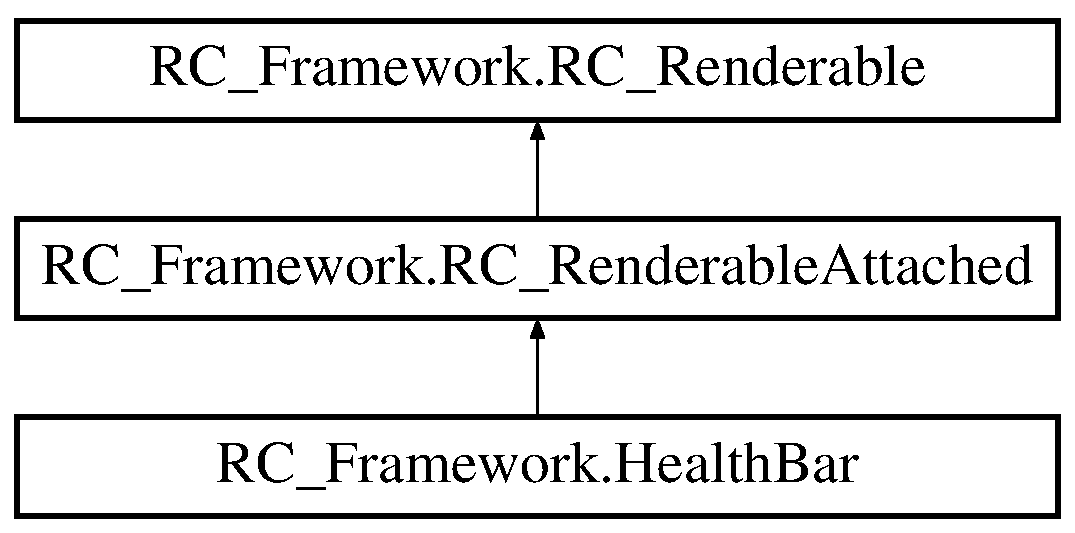
\includegraphics[height=3.000000cm]{class_r_c___framework_1_1_health_bar}
\end{center}
\end{figure}
\subsection*{Public Member Functions}
\begin{DoxyCompactItemize}
\item 
\mbox{\hyperlink{class_r_c___framework_1_1_health_bar_a1fadf428d30ca6fc622be62ae38c0fb4}{Health\+Bar}} (Color bar, Color back\+Ground, Color bar\+Off\+ColorZ, int heightZ, bool always\+DrawZ)
\item 
override void \mbox{\hyperlink{class_r_c___framework_1_1_health_bar_a8f53c56c52544e3c257db3d698fd2926}{Draw}} (Sprite\+Batch sb)
\begin{DoxyCompactList}\small\item\em Standard draw routine which assumes the renderable knows where it is \end{DoxyCompactList}\end{DoxyCompactItemize}
\subsection*{Additional Inherited Members}


\subsection{Detailed Description}
healthbar class to attach to sprite set alwaysdraw to true if you wan the bar at all times set it to false if you want it only when damaged 



\subsection{Constructor \& Destructor Documentation}
\mbox{\Hypertarget{class_r_c___framework_1_1_health_bar_a1fadf428d30ca6fc622be62ae38c0fb4}\label{class_r_c___framework_1_1_health_bar_a1fadf428d30ca6fc622be62ae38c0fb4}} 
\index{R\+C\+\_\+\+Framework\+::\+Health\+Bar@{R\+C\+\_\+\+Framework\+::\+Health\+Bar}!Health\+Bar@{Health\+Bar}}
\index{Health\+Bar@{Health\+Bar}!R\+C\+\_\+\+Framework\+::\+Health\+Bar@{R\+C\+\_\+\+Framework\+::\+Health\+Bar}}
\subsubsection{\texorpdfstring{Health\+Bar()}{HealthBar()}}
{\footnotesize\ttfamily R\+C\+\_\+\+Framework.\+Health\+Bar.\+Health\+Bar (\begin{DoxyParamCaption}\item[{Color}]{bar,  }\item[{Color}]{back\+Ground,  }\item[{Color}]{bar\+Off\+ColorZ,  }\item[{int}]{heightZ,  }\item[{bool}]{always\+DrawZ }\end{DoxyParamCaption})}



\subsection{Member Function Documentation}
\mbox{\Hypertarget{class_r_c___framework_1_1_health_bar_a8f53c56c52544e3c257db3d698fd2926}\label{class_r_c___framework_1_1_health_bar_a8f53c56c52544e3c257db3d698fd2926}} 
\index{R\+C\+\_\+\+Framework\+::\+Health\+Bar@{R\+C\+\_\+\+Framework\+::\+Health\+Bar}!Draw@{Draw}}
\index{Draw@{Draw}!R\+C\+\_\+\+Framework\+::\+Health\+Bar@{R\+C\+\_\+\+Framework\+::\+Health\+Bar}}
\subsubsection{\texorpdfstring{Draw()}{Draw()}}
{\footnotesize\ttfamily override void R\+C\+\_\+\+Framework.\+Health\+Bar.\+Draw (\begin{DoxyParamCaption}\item[{Sprite\+Batch}]{sb }\end{DoxyParamCaption})\hspace{0.3cm}{\ttfamily [virtual]}}



Standard draw routine which assumes the renderable knows where it is 


\begin{DoxyParams}{Parameters}
{\em sb} & \\
\hline
\end{DoxyParams}


Reimplemented from \mbox{\hyperlink{class_r_c___framework_1_1_r_c___renderable_acc26db34e382a25a989c4c0dd0354b23}{R\+C\+\_\+\+Framework.\+R\+C\+\_\+\+Renderable}}.



The documentation for this class was generated from the following file\+:\begin{DoxyCompactItemize}
\item 
F\+:/\+B/\+R\+C\+\_\+\+Framework2018/\+Source/\mbox{\hyperlink{_r_c___renderable_attached_8cs}{R\+C\+\_\+\+Renderable\+Attached.\+cs}}\end{DoxyCompactItemize}

\hypertarget{class_r_c___framework_1_1_image_background}{}\section{R\+C\+\_\+\+Framework.\+Image\+Background Class Reference}
\label{class_r_c___framework_1_1_image_background}\index{R\+C\+\_\+\+Framework.\+Image\+Background@{R\+C\+\_\+\+Framework.\+Image\+Background}}


A background image with source, colour and destination Can Automatically resize to viewport consequently it needs the viewport passed in by graphics device If the source is null the whole texture is used  


Inheritance diagram for R\+C\+\_\+\+Framework.\+Image\+Background\+:\begin{figure}[H]
\begin{center}
\leavevmode
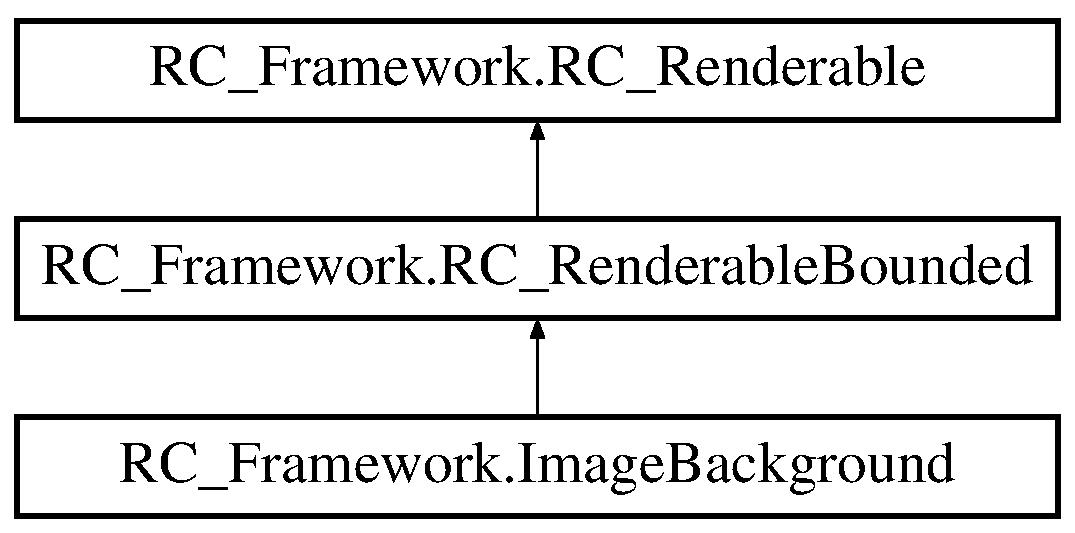
\includegraphics[height=3.000000cm]{class_r_c___framework_1_1_image_background}
\end{center}
\end{figure}
\subsection*{Public Member Functions}
\begin{DoxyCompactItemize}
\item 
\mbox{\hyperlink{class_r_c___framework_1_1_image_background_ad66973504fc9518e98e0757458973880}{Image\+Background}} (Texture2D texZ, Rectangle? sourceZ, Rectangle destZ, Color colourZ)
\item 
\mbox{\hyperlink{class_r_c___framework_1_1_image_background_a64185561061a54b6241c982541ed54a7}{Image\+Background}} (Texture2D texZ, Color colourZ, Graphics\+Device g)
\item 
override void \mbox{\hyperlink{class_r_c___framework_1_1_image_background_a1aaef38a9b320b21dc558e25d5a4c0af}{Draw}} (Sprite\+Batch sb)
\begin{DoxyCompactList}\small\item\em Standard draw routine which assumes the renderable knows where it is \end{DoxyCompactList}\end{DoxyCompactItemize}
\subsection*{Properties}
\begin{DoxyCompactItemize}
\item 
Texture2D \mbox{\hyperlink{class_r_c___framework_1_1_image_background_acbae55d0eec7e9db3b3dd1e6adcbd01e}{tex}}\hspace{0.3cm}{\ttfamily  \mbox{[}get, set\mbox{]}}
\item 
Rectangle \mbox{\hyperlink{class_r_c___framework_1_1_image_background_a58fe22eaa5ab35456cd3a1d8c4b06295}{source}}\hspace{0.3cm}{\ttfamily  \mbox{[}get, set\mbox{]}}
\end{DoxyCompactItemize}
\subsection*{Additional Inherited Members}


\subsection{Detailed Description}
A background image with source, colour and destination Can Automatically resize to viewport consequently it needs the viewport passed in by graphics device If the source is null the whole texture is used 



\subsection{Constructor \& Destructor Documentation}
\mbox{\Hypertarget{class_r_c___framework_1_1_image_background_ad66973504fc9518e98e0757458973880}\label{class_r_c___framework_1_1_image_background_ad66973504fc9518e98e0757458973880}} 
\index{R\+C\+\_\+\+Framework\+::\+Image\+Background@{R\+C\+\_\+\+Framework\+::\+Image\+Background}!Image\+Background@{Image\+Background}}
\index{Image\+Background@{Image\+Background}!R\+C\+\_\+\+Framework\+::\+Image\+Background@{R\+C\+\_\+\+Framework\+::\+Image\+Background}}
\subsubsection{\texorpdfstring{Image\+Background()}{ImageBackground()}\hspace{0.1cm}{\footnotesize\ttfamily [1/2]}}
{\footnotesize\ttfamily R\+C\+\_\+\+Framework.\+Image\+Background.\+Image\+Background (\begin{DoxyParamCaption}\item[{Texture2D}]{texZ,  }\item[{Rectangle?}]{sourceZ,  }\item[{Rectangle}]{destZ,  }\item[{Color}]{colourZ }\end{DoxyParamCaption})}

\mbox{\Hypertarget{class_r_c___framework_1_1_image_background_a64185561061a54b6241c982541ed54a7}\label{class_r_c___framework_1_1_image_background_a64185561061a54b6241c982541ed54a7}} 
\index{R\+C\+\_\+\+Framework\+::\+Image\+Background@{R\+C\+\_\+\+Framework\+::\+Image\+Background}!Image\+Background@{Image\+Background}}
\index{Image\+Background@{Image\+Background}!R\+C\+\_\+\+Framework\+::\+Image\+Background@{R\+C\+\_\+\+Framework\+::\+Image\+Background}}
\subsubsection{\texorpdfstring{Image\+Background()}{ImageBackground()}\hspace{0.1cm}{\footnotesize\ttfamily [2/2]}}
{\footnotesize\ttfamily R\+C\+\_\+\+Framework.\+Image\+Background.\+Image\+Background (\begin{DoxyParamCaption}\item[{Texture2D}]{texZ,  }\item[{Color}]{colourZ,  }\item[{Graphics\+Device}]{g }\end{DoxyParamCaption})}



\subsection{Member Function Documentation}
\mbox{\Hypertarget{class_r_c___framework_1_1_image_background_a1aaef38a9b320b21dc558e25d5a4c0af}\label{class_r_c___framework_1_1_image_background_a1aaef38a9b320b21dc558e25d5a4c0af}} 
\index{R\+C\+\_\+\+Framework\+::\+Image\+Background@{R\+C\+\_\+\+Framework\+::\+Image\+Background}!Draw@{Draw}}
\index{Draw@{Draw}!R\+C\+\_\+\+Framework\+::\+Image\+Background@{R\+C\+\_\+\+Framework\+::\+Image\+Background}}
\subsubsection{\texorpdfstring{Draw()}{Draw()}}
{\footnotesize\ttfamily override void R\+C\+\_\+\+Framework.\+Image\+Background.\+Draw (\begin{DoxyParamCaption}\item[{Sprite\+Batch}]{sb }\end{DoxyParamCaption})\hspace{0.3cm}{\ttfamily [virtual]}}



Standard draw routine which assumes the renderable knows where it is 


\begin{DoxyParams}{Parameters}
{\em sb} & \\
\hline
\end{DoxyParams}


Reimplemented from \mbox{\hyperlink{class_r_c___framework_1_1_r_c___renderable_acc26db34e382a25a989c4c0dd0354b23}{R\+C\+\_\+\+Framework.\+R\+C\+\_\+\+Renderable}}.



\subsection{Property Documentation}
\mbox{\Hypertarget{class_r_c___framework_1_1_image_background_a58fe22eaa5ab35456cd3a1d8c4b06295}\label{class_r_c___framework_1_1_image_background_a58fe22eaa5ab35456cd3a1d8c4b06295}} 
\index{R\+C\+\_\+\+Framework\+::\+Image\+Background@{R\+C\+\_\+\+Framework\+::\+Image\+Background}!source@{source}}
\index{source@{source}!R\+C\+\_\+\+Framework\+::\+Image\+Background@{R\+C\+\_\+\+Framework\+::\+Image\+Background}}
\subsubsection{\texorpdfstring{source}{source}}
{\footnotesize\ttfamily Rectangle R\+C\+\_\+\+Framework.\+Image\+Background.\+source\hspace{0.3cm}{\ttfamily [get]}, {\ttfamily [set]}}

\mbox{\Hypertarget{class_r_c___framework_1_1_image_background_acbae55d0eec7e9db3b3dd1e6adcbd01e}\label{class_r_c___framework_1_1_image_background_acbae55d0eec7e9db3b3dd1e6adcbd01e}} 
\index{R\+C\+\_\+\+Framework\+::\+Image\+Background@{R\+C\+\_\+\+Framework\+::\+Image\+Background}!tex@{tex}}
\index{tex@{tex}!R\+C\+\_\+\+Framework\+::\+Image\+Background@{R\+C\+\_\+\+Framework\+::\+Image\+Background}}
\subsubsection{\texorpdfstring{tex}{tex}}
{\footnotesize\ttfamily Texture2D R\+C\+\_\+\+Framework.\+Image\+Background.\+tex\hspace{0.3cm}{\ttfamily [get]}, {\ttfamily [set]}}



The documentation for this class was generated from the following file\+:\begin{DoxyCompactItemize}
\item 
F\+:/\+B/\+R\+C\+\_\+\+Framework2018/\+Source/\mbox{\hyperlink{_r_c___renderable_bounded_8cs}{R\+C\+\_\+\+Renderable\+Bounded.\+cs}}\end{DoxyCompactItemize}

\hypertarget{class_r_c___framework_1_1_input_box}{}\section{R\+C\+\_\+\+Framework.\+Input\+Box Class Reference}
\label{class_r_c___framework_1_1_input_box}\index{R\+C\+\_\+\+Framework.\+Input\+Box@{R\+C\+\_\+\+Framework.\+Input\+Box}}


get the text from the user  


Inheritance diagram for R\+C\+\_\+\+Framework.\+Input\+Box\+:\begin{figure}[H]
\begin{center}
\leavevmode
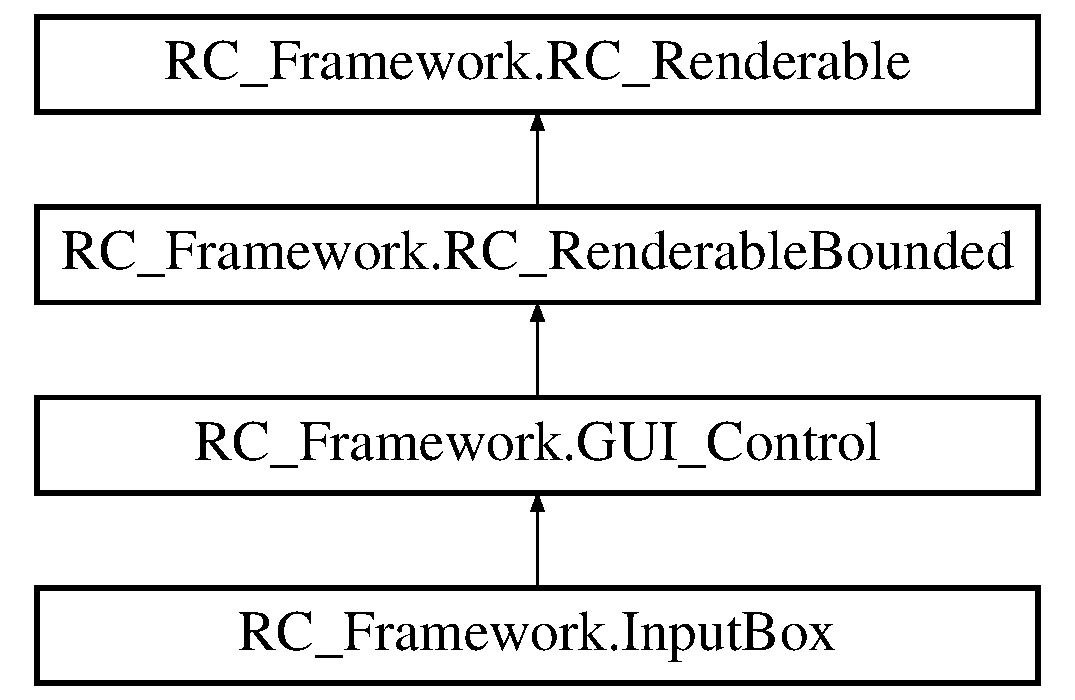
\includegraphics[height=4.000000cm]{class_r_c___framework_1_1_input_box}
\end{center}
\end{figure}
\subsection*{Public Member Functions}
\begin{DoxyCompactItemize}
\item 
\mbox{\hyperlink{class_r_c___framework_1_1_input_box_ad692dce3ce7a7a99916b510aa88b9354}{Input\+Box}} (Texture2D texZ, Vector2 pos, Sprite\+Font fonty, string s, int max\+Len)
\begin{DoxyCompactList}\small\item\em \mbox{\hyperlink{class_r_c___framework_1_1_input_box}{Input\+Box}} constructor resizes to image width \end{DoxyCompactList}\item 
\mbox{\hyperlink{class_r_c___framework_1_1_input_box_ab33c6d6a73473a9067093deb2c95b865}{Input\+Box}} (Texture2D texZ, Rectangle pos, Sprite\+Font fonty, string s, int max\+Len)
\begin{DoxyCompactList}\small\item\em \mbox{\hyperlink{class_r_c___framework_1_1_input_box}{Input\+Box}} constructor \end{DoxyCompactList}\item 
int \mbox{\hyperlink{class_r_c___framework_1_1_input_box_a536e557732c8a9d599c8c5190410738f}{as\+Integer}} ()
\begin{DoxyCompactList}\small\item\em Get the text as an integer \end{DoxyCompactList}\item 
override void \mbox{\hyperlink{class_r_c___framework_1_1_input_box_ae5ee048852636d3675318a630cfc0ec6}{Draw}} (Sprite\+Batch sb)
\begin{DoxyCompactList}\small\item\em We all know Draw \end{DoxyCompactList}\item 
override void \mbox{\hyperlink{class_r_c___framework_1_1_input_box_ac91004a57916d0f9f55a40c007cb72ce}{Update}} (Game\+Time game\+Time)
\begin{DoxyCompactList}\small\item\em Upadte \end{DoxyCompactList}\item 
override bool \mbox{\hyperlink{class_r_c___framework_1_1_input_box_a07ef881a281e4da95994e54ec1f7b496}{Key\+Hit\+Event}} (Keys key)
\begin{DoxyCompactList}\small\item\em Handle key hit \end{DoxyCompactList}\item 
override bool \mbox{\hyperlink{class_r_c___framework_1_1_input_box_a7e57c860483df9645d726d6adbbc6dab}{Mouse\+Down\+Event\+Left}} (float mouse\+\_\+x, float mouse\+\_\+y)
\begin{DoxyCompactList}\small\item\em handle mouse down \end{DoxyCompactList}\end{DoxyCompactItemize}
\subsection*{Public Attributes}
\begin{DoxyCompactItemize}
\item 
Vector2 \mbox{\hyperlink{class_r_c___framework_1_1_input_box_a96345a99971dd664242c1f9c1e0231a7}{text\+Offset}}
\begin{DoxyCompactList}\small\item\em where to display the text \end{DoxyCompactList}\end{DoxyCompactItemize}
\subsection*{Additional Inherited Members}


\subsection{Detailed Description}
get the text from the user 



\subsection{Constructor \& Destructor Documentation}
\mbox{\Hypertarget{class_r_c___framework_1_1_input_box_ad692dce3ce7a7a99916b510aa88b9354}\label{class_r_c___framework_1_1_input_box_ad692dce3ce7a7a99916b510aa88b9354}} 
\index{R\+C\+\_\+\+Framework\+::\+Input\+Box@{R\+C\+\_\+\+Framework\+::\+Input\+Box}!Input\+Box@{Input\+Box}}
\index{Input\+Box@{Input\+Box}!R\+C\+\_\+\+Framework\+::\+Input\+Box@{R\+C\+\_\+\+Framework\+::\+Input\+Box}}
\subsubsection{\texorpdfstring{Input\+Box()}{InputBox()}\hspace{0.1cm}{\footnotesize\ttfamily [1/2]}}
{\footnotesize\ttfamily R\+C\+\_\+\+Framework.\+Input\+Box.\+Input\+Box (\begin{DoxyParamCaption}\item[{Texture2D}]{texZ,  }\item[{Vector2}]{pos,  }\item[{Sprite\+Font}]{fonty,  }\item[{string}]{s,  }\item[{int}]{max\+Len }\end{DoxyParamCaption})}



\mbox{\hyperlink{class_r_c___framework_1_1_input_box}{Input\+Box}} constructor resizes to image width 


\begin{DoxyParams}{Parameters}
{\em texZ} & \\
\hline
{\em pos} & \\
\hline
{\em fonty} & \\
\hline
{\em s} & \\
\hline
{\em max\+Len} & \\
\hline
\end{DoxyParams}
\mbox{\Hypertarget{class_r_c___framework_1_1_input_box_ab33c6d6a73473a9067093deb2c95b865}\label{class_r_c___framework_1_1_input_box_ab33c6d6a73473a9067093deb2c95b865}} 
\index{R\+C\+\_\+\+Framework\+::\+Input\+Box@{R\+C\+\_\+\+Framework\+::\+Input\+Box}!Input\+Box@{Input\+Box}}
\index{Input\+Box@{Input\+Box}!R\+C\+\_\+\+Framework\+::\+Input\+Box@{R\+C\+\_\+\+Framework\+::\+Input\+Box}}
\subsubsection{\texorpdfstring{Input\+Box()}{InputBox()}\hspace{0.1cm}{\footnotesize\ttfamily [2/2]}}
{\footnotesize\ttfamily R\+C\+\_\+\+Framework.\+Input\+Box.\+Input\+Box (\begin{DoxyParamCaption}\item[{Texture2D}]{texZ,  }\item[{Rectangle}]{pos,  }\item[{Sprite\+Font}]{fonty,  }\item[{string}]{s,  }\item[{int}]{max\+Len }\end{DoxyParamCaption})}



\mbox{\hyperlink{class_r_c___framework_1_1_input_box}{Input\+Box}} constructor 


\begin{DoxyParams}{Parameters}
{\em texZ} & \\
\hline
{\em pos} & \\
\hline
{\em fonty} & \\
\hline
{\em s} & \\
\hline
{\em max\+Len} & \\
\hline
\end{DoxyParams}


\subsection{Member Function Documentation}
\mbox{\Hypertarget{class_r_c___framework_1_1_input_box_a536e557732c8a9d599c8c5190410738f}\label{class_r_c___framework_1_1_input_box_a536e557732c8a9d599c8c5190410738f}} 
\index{R\+C\+\_\+\+Framework\+::\+Input\+Box@{R\+C\+\_\+\+Framework\+::\+Input\+Box}!as\+Integer@{as\+Integer}}
\index{as\+Integer@{as\+Integer}!R\+C\+\_\+\+Framework\+::\+Input\+Box@{R\+C\+\_\+\+Framework\+::\+Input\+Box}}
\subsubsection{\texorpdfstring{as\+Integer()}{asInteger()}}
{\footnotesize\ttfamily int R\+C\+\_\+\+Framework.\+Input\+Box.\+as\+Integer (\begin{DoxyParamCaption}{ }\end{DoxyParamCaption})}



Get the text as an integer 

\begin{DoxyReturn}{Returns}

\end{DoxyReturn}
\mbox{\Hypertarget{class_r_c___framework_1_1_input_box_ae5ee048852636d3675318a630cfc0ec6}\label{class_r_c___framework_1_1_input_box_ae5ee048852636d3675318a630cfc0ec6}} 
\index{R\+C\+\_\+\+Framework\+::\+Input\+Box@{R\+C\+\_\+\+Framework\+::\+Input\+Box}!Draw@{Draw}}
\index{Draw@{Draw}!R\+C\+\_\+\+Framework\+::\+Input\+Box@{R\+C\+\_\+\+Framework\+::\+Input\+Box}}
\subsubsection{\texorpdfstring{Draw()}{Draw()}}
{\footnotesize\ttfamily override void R\+C\+\_\+\+Framework.\+Input\+Box.\+Draw (\begin{DoxyParamCaption}\item[{Sprite\+Batch}]{sb }\end{DoxyParamCaption})\hspace{0.3cm}{\ttfamily [virtual]}}



We all know Draw 


\begin{DoxyParams}{Parameters}
{\em sb} & \\
\hline
\end{DoxyParams}


Reimplemented from \mbox{\hyperlink{class_r_c___framework_1_1_r_c___renderable_acc26db34e382a25a989c4c0dd0354b23}{R\+C\+\_\+\+Framework.\+R\+C\+\_\+\+Renderable}}.

\mbox{\Hypertarget{class_r_c___framework_1_1_input_box_a07ef881a281e4da95994e54ec1f7b496}\label{class_r_c___framework_1_1_input_box_a07ef881a281e4da95994e54ec1f7b496}} 
\index{R\+C\+\_\+\+Framework\+::\+Input\+Box@{R\+C\+\_\+\+Framework\+::\+Input\+Box}!Key\+Hit\+Event@{Key\+Hit\+Event}}
\index{Key\+Hit\+Event@{Key\+Hit\+Event}!R\+C\+\_\+\+Framework\+::\+Input\+Box@{R\+C\+\_\+\+Framework\+::\+Input\+Box}}
\subsubsection{\texorpdfstring{Key\+Hit\+Event()}{KeyHitEvent()}}
{\footnotesize\ttfamily override bool R\+C\+\_\+\+Framework.\+Input\+Box.\+Key\+Hit\+Event (\begin{DoxyParamCaption}\item[{Keys}]{key }\end{DoxyParamCaption})\hspace{0.3cm}{\ttfamily [virtual]}}



Handle key hit 


\begin{DoxyParams}{Parameters}
{\em key} & \\
\hline
\end{DoxyParams}
\begin{DoxyReturn}{Returns}

\end{DoxyReturn}


Reimplemented from \mbox{\hyperlink{class_r_c___framework_1_1_g_u_i___control_a458eb00bda180db22ebe22e550a669a4}{R\+C\+\_\+\+Framework.\+G\+U\+I\+\_\+\+Control}}.

\mbox{\Hypertarget{class_r_c___framework_1_1_input_box_a7e57c860483df9645d726d6adbbc6dab}\label{class_r_c___framework_1_1_input_box_a7e57c860483df9645d726d6adbbc6dab}} 
\index{R\+C\+\_\+\+Framework\+::\+Input\+Box@{R\+C\+\_\+\+Framework\+::\+Input\+Box}!Mouse\+Down\+Event\+Left@{Mouse\+Down\+Event\+Left}}
\index{Mouse\+Down\+Event\+Left@{Mouse\+Down\+Event\+Left}!R\+C\+\_\+\+Framework\+::\+Input\+Box@{R\+C\+\_\+\+Framework\+::\+Input\+Box}}
\subsubsection{\texorpdfstring{Mouse\+Down\+Event\+Left()}{MouseDownEventLeft()}}
{\footnotesize\ttfamily override bool R\+C\+\_\+\+Framework.\+Input\+Box.\+Mouse\+Down\+Event\+Left (\begin{DoxyParamCaption}\item[{float}]{mouse\+\_\+x,  }\item[{float}]{mouse\+\_\+y }\end{DoxyParamCaption})\hspace{0.3cm}{\ttfamily [virtual]}}



handle mouse down 


\begin{DoxyParams}{Parameters}
{\em mouse\+\_\+x} & \\
\hline
{\em mouse\+\_\+y} & \\
\hline
\end{DoxyParams}
\begin{DoxyReturn}{Returns}

\end{DoxyReturn}


Reimplemented from \mbox{\hyperlink{class_r_c___framework_1_1_g_u_i___control_a005e7f109afd21abd6576fdf70212af5}{R\+C\+\_\+\+Framework.\+G\+U\+I\+\_\+\+Control}}.

\mbox{\Hypertarget{class_r_c___framework_1_1_input_box_ac91004a57916d0f9f55a40c007cb72ce}\label{class_r_c___framework_1_1_input_box_ac91004a57916d0f9f55a40c007cb72ce}} 
\index{R\+C\+\_\+\+Framework\+::\+Input\+Box@{R\+C\+\_\+\+Framework\+::\+Input\+Box}!Update@{Update}}
\index{Update@{Update}!R\+C\+\_\+\+Framework\+::\+Input\+Box@{R\+C\+\_\+\+Framework\+::\+Input\+Box}}
\subsubsection{\texorpdfstring{Update()}{Update()}}
{\footnotesize\ttfamily override void R\+C\+\_\+\+Framework.\+Input\+Box.\+Update (\begin{DoxyParamCaption}\item[{Game\+Time}]{game\+Time }\end{DoxyParamCaption})\hspace{0.3cm}{\ttfamily [virtual]}}



Upadte 


\begin{DoxyParams}{Parameters}
{\em game\+Time} & \\
\hline
\end{DoxyParams}


Reimplemented from \mbox{\hyperlink{class_r_c___framework_1_1_g_u_i___control_a7aa3b0b6ba141d995ca830ff99ae3003}{R\+C\+\_\+\+Framework.\+G\+U\+I\+\_\+\+Control}}.



\subsection{Member Data Documentation}
\mbox{\Hypertarget{class_r_c___framework_1_1_input_box_a96345a99971dd664242c1f9c1e0231a7}\label{class_r_c___framework_1_1_input_box_a96345a99971dd664242c1f9c1e0231a7}} 
\index{R\+C\+\_\+\+Framework\+::\+Input\+Box@{R\+C\+\_\+\+Framework\+::\+Input\+Box}!text\+Offset@{text\+Offset}}
\index{text\+Offset@{text\+Offset}!R\+C\+\_\+\+Framework\+::\+Input\+Box@{R\+C\+\_\+\+Framework\+::\+Input\+Box}}
\subsubsection{\texorpdfstring{text\+Offset}{textOffset}}
{\footnotesize\ttfamily Vector2 R\+C\+\_\+\+Framework.\+Input\+Box.\+text\+Offset}



where to display the text 



The documentation for this class was generated from the following file\+:\begin{DoxyCompactItemize}
\item 
F\+:/\+B/\+R\+C\+\_\+\+Framework2018/\+Source/\mbox{\hyperlink{_r_c___g_u_i_8cs}{R\+C\+\_\+\+G\+U\+I.\+cs}}\end{DoxyCompactItemize}

\hypertarget{class_r_c___framework_1_1_texture_flash_1_1_letterbox_mask}{}\section{R\+C\+\_\+\+Framework.\+Texture\+Flash.\+Letterbox\+Mask Class Reference}
\label{class_r_c___framework_1_1_texture_flash_1_1_letterbox_mask}\index{R\+C\+\_\+\+Framework.\+Texture\+Flash.\+Letterbox\+Mask@{R\+C\+\_\+\+Framework.\+Texture\+Flash.\+Letterbox\+Mask}}
Inheritance diagram for R\+C\+\_\+\+Framework.\+Texture\+Flash.\+Letterbox\+Mask\+:\begin{figure}[H]
\begin{center}
\leavevmode
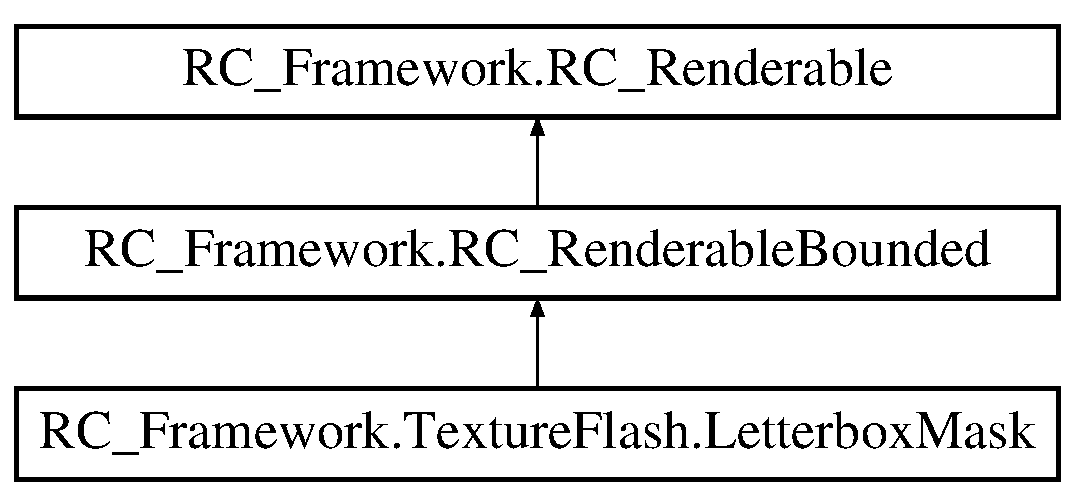
\includegraphics[height=3.000000cm]{class_r_c___framework_1_1_texture_flash_1_1_letterbox_mask}
\end{center}
\end{figure}
\subsection*{Public Member Functions}
\begin{DoxyCompactItemize}
\item 
\mbox{\hyperlink{class_r_c___framework_1_1_texture_flash_1_1_letterbox_mask_a5b9e168c4c83a61ed8a42dbc5ded5425}{Letterbox\+Mask}} (Rectangle outer\+RectangleQ, int width\+Of\+MaskQ, Color mask\+ColorQ)
\item 
override void \mbox{\hyperlink{class_r_c___framework_1_1_texture_flash_1_1_letterbox_mask_aadd01ce0789efac12bc044f336bb5b33}{Draw}} (Sprite\+Batch sb)
\begin{DoxyCompactList}\small\item\em Standard draw routine which assumes the renderable knows where it is \end{DoxyCompactList}\end{DoxyCompactItemize}
\subsection*{Additional Inherited Members}


\subsection{Constructor \& Destructor Documentation}
\mbox{\Hypertarget{class_r_c___framework_1_1_texture_flash_1_1_letterbox_mask_a5b9e168c4c83a61ed8a42dbc5ded5425}\label{class_r_c___framework_1_1_texture_flash_1_1_letterbox_mask_a5b9e168c4c83a61ed8a42dbc5ded5425}} 
\index{R\+C\+\_\+\+Framework\+::\+Texture\+Flash\+::\+Letterbox\+Mask@{R\+C\+\_\+\+Framework\+::\+Texture\+Flash\+::\+Letterbox\+Mask}!Letterbox\+Mask@{Letterbox\+Mask}}
\index{Letterbox\+Mask@{Letterbox\+Mask}!R\+C\+\_\+\+Framework\+::\+Texture\+Flash\+::\+Letterbox\+Mask@{R\+C\+\_\+\+Framework\+::\+Texture\+Flash\+::\+Letterbox\+Mask}}
\subsubsection{\texorpdfstring{Letterbox\+Mask()}{LetterboxMask()}}
{\footnotesize\ttfamily R\+C\+\_\+\+Framework.\+Texture\+Flash.\+Letterbox\+Mask.\+Letterbox\+Mask (\begin{DoxyParamCaption}\item[{Rectangle}]{outer\+RectangleQ,  }\item[{int}]{width\+Of\+MaskQ,  }\item[{Color}]{mask\+ColorQ }\end{DoxyParamCaption})}



\subsection{Member Function Documentation}
\mbox{\Hypertarget{class_r_c___framework_1_1_texture_flash_1_1_letterbox_mask_aadd01ce0789efac12bc044f336bb5b33}\label{class_r_c___framework_1_1_texture_flash_1_1_letterbox_mask_aadd01ce0789efac12bc044f336bb5b33}} 
\index{R\+C\+\_\+\+Framework\+::\+Texture\+Flash\+::\+Letterbox\+Mask@{R\+C\+\_\+\+Framework\+::\+Texture\+Flash\+::\+Letterbox\+Mask}!Draw@{Draw}}
\index{Draw@{Draw}!R\+C\+\_\+\+Framework\+::\+Texture\+Flash\+::\+Letterbox\+Mask@{R\+C\+\_\+\+Framework\+::\+Texture\+Flash\+::\+Letterbox\+Mask}}
\subsubsection{\texorpdfstring{Draw()}{Draw()}}
{\footnotesize\ttfamily override void R\+C\+\_\+\+Framework.\+Texture\+Flash.\+Letterbox\+Mask.\+Draw (\begin{DoxyParamCaption}\item[{Sprite\+Batch}]{sb }\end{DoxyParamCaption})\hspace{0.3cm}{\ttfamily [virtual]}}



Standard draw routine which assumes the renderable knows where it is 


\begin{DoxyParams}{Parameters}
{\em sb} & \\
\hline
\end{DoxyParams}


Reimplemented from \mbox{\hyperlink{class_r_c___framework_1_1_r_c___renderable_acc26db34e382a25a989c4c0dd0354b23}{R\+C\+\_\+\+Framework.\+R\+C\+\_\+\+Renderable}}.



The documentation for this class was generated from the following file\+:\begin{DoxyCompactItemize}
\item 
F\+:/\+B/\+R\+C\+\_\+\+Framework2018/\+Source/\mbox{\hyperlink{_r_c___renderable_bounded_8cs}{R\+C\+\_\+\+Renderable\+Bounded.\+cs}}\end{DoxyCompactItemize}

\hypertarget{class_r_c___framework_1_1_limit_sound}{}\section{R\+C\+\_\+\+Framework.\+Limit\+Sound Class Reference}
\label{class_r_c___framework_1_1_limit_sound}\index{R\+C\+\_\+\+Framework.\+Limit\+Sound@{R\+C\+\_\+\+Framework.\+Limit\+Sound}}


Limits a sound to playing a certian number of instances of itself (stops muddy sound) Warning this needs a call in Update  


\subsection*{Public Member Functions}
\begin{DoxyCompactItemize}
\item 
\mbox{\hyperlink{class_r_c___framework_1_1_limit_sound_a9cbeff174c2bb2fcaac7787b744feed8}{Limit\+Sound}} (Sound\+Effect sound\+Effect, int num\+Of\+Soundz)
\begin{DoxyCompactList}\small\item\em Create it using a soundeffect \end{DoxyCompactList}\item 
\mbox{\hyperlink{class_r_c___framework_1_1_limit_sound_a44dfcf8fbf1e0ba71457097f7f32176e}{Limit\+Sound}} (string name, int num\+Of\+Soundz, Content\+Manager c)
\begin{DoxyCompactList}\small\item\em create it using a sound name \end{DoxyCompactList}\item 
void \mbox{\hyperlink{class_r_c___framework_1_1_limit_sound_a17847d5b1d8c9c55b66a274e0e7e22cc}{play\+Sound}} ()
\begin{DoxyCompactList}\small\item\em play the sound from the start \end{DoxyCompactList}\item 
void \mbox{\hyperlink{class_r_c___framework_1_1_limit_sound_a0d63e6c2b23828bf2b570c55f2fa396a}{play\+Sound\+If\+Ok}} ()
\begin{DoxyCompactList}\small\item\em Play it only if one is not already playing \end{DoxyCompactList}\item 
void \mbox{\hyperlink{class_r_c___framework_1_1_limit_sound_a9d6eda93ccf422244fbe7a9ca2a19f13}{Update}} (Game\+Time game\+Time)
\end{DoxyCompactItemize}


\subsection{Detailed Description}
Limits a sound to playing a certian number of instances of itself (stops muddy sound) Warning this needs a call in Update 



\subsection{Constructor \& Destructor Documentation}
\mbox{\Hypertarget{class_r_c___framework_1_1_limit_sound_a9cbeff174c2bb2fcaac7787b744feed8}\label{class_r_c___framework_1_1_limit_sound_a9cbeff174c2bb2fcaac7787b744feed8}} 
\index{R\+C\+\_\+\+Framework\+::\+Limit\+Sound@{R\+C\+\_\+\+Framework\+::\+Limit\+Sound}!Limit\+Sound@{Limit\+Sound}}
\index{Limit\+Sound@{Limit\+Sound}!R\+C\+\_\+\+Framework\+::\+Limit\+Sound@{R\+C\+\_\+\+Framework\+::\+Limit\+Sound}}
\subsubsection{\texorpdfstring{Limit\+Sound()}{LimitSound()}\hspace{0.1cm}{\footnotesize\ttfamily [1/2]}}
{\footnotesize\ttfamily R\+C\+\_\+\+Framework.\+Limit\+Sound.\+Limit\+Sound (\begin{DoxyParamCaption}\item[{Sound\+Effect}]{sound\+Effect,  }\item[{int}]{num\+Of\+Soundz }\end{DoxyParamCaption})}



Create it using a soundeffect 


\begin{DoxyParams}{Parameters}
{\em sound\+Effect} & \\
\hline
{\em num\+Of\+Soundz} & \\
\hline
\end{DoxyParams}
\mbox{\Hypertarget{class_r_c___framework_1_1_limit_sound_a44dfcf8fbf1e0ba71457097f7f32176e}\label{class_r_c___framework_1_1_limit_sound_a44dfcf8fbf1e0ba71457097f7f32176e}} 
\index{R\+C\+\_\+\+Framework\+::\+Limit\+Sound@{R\+C\+\_\+\+Framework\+::\+Limit\+Sound}!Limit\+Sound@{Limit\+Sound}}
\index{Limit\+Sound@{Limit\+Sound}!R\+C\+\_\+\+Framework\+::\+Limit\+Sound@{R\+C\+\_\+\+Framework\+::\+Limit\+Sound}}
\subsubsection{\texorpdfstring{Limit\+Sound()}{LimitSound()}\hspace{0.1cm}{\footnotesize\ttfamily [2/2]}}
{\footnotesize\ttfamily R\+C\+\_\+\+Framework.\+Limit\+Sound.\+Limit\+Sound (\begin{DoxyParamCaption}\item[{string}]{name,  }\item[{int}]{num\+Of\+Soundz,  }\item[{Content\+Manager}]{c }\end{DoxyParamCaption})}



create it using a sound name 


\begin{DoxyParams}{Parameters}
{\em name} & \\
\hline
{\em num\+Of\+Soundz} & \\
\hline
{\em c} & \\
\hline
\end{DoxyParams}


\subsection{Member Function Documentation}
\mbox{\Hypertarget{class_r_c___framework_1_1_limit_sound_a17847d5b1d8c9c55b66a274e0e7e22cc}\label{class_r_c___framework_1_1_limit_sound_a17847d5b1d8c9c55b66a274e0e7e22cc}} 
\index{R\+C\+\_\+\+Framework\+::\+Limit\+Sound@{R\+C\+\_\+\+Framework\+::\+Limit\+Sound}!play\+Sound@{play\+Sound}}
\index{play\+Sound@{play\+Sound}!R\+C\+\_\+\+Framework\+::\+Limit\+Sound@{R\+C\+\_\+\+Framework\+::\+Limit\+Sound}}
\subsubsection{\texorpdfstring{play\+Sound()}{playSound()}}
{\footnotesize\ttfamily void R\+C\+\_\+\+Framework.\+Limit\+Sound.\+play\+Sound (\begin{DoxyParamCaption}{ }\end{DoxyParamCaption})}



play the sound from the start 

\mbox{\Hypertarget{class_r_c___framework_1_1_limit_sound_a0d63e6c2b23828bf2b570c55f2fa396a}\label{class_r_c___framework_1_1_limit_sound_a0d63e6c2b23828bf2b570c55f2fa396a}} 
\index{R\+C\+\_\+\+Framework\+::\+Limit\+Sound@{R\+C\+\_\+\+Framework\+::\+Limit\+Sound}!play\+Sound\+If\+Ok@{play\+Sound\+If\+Ok}}
\index{play\+Sound\+If\+Ok@{play\+Sound\+If\+Ok}!R\+C\+\_\+\+Framework\+::\+Limit\+Sound@{R\+C\+\_\+\+Framework\+::\+Limit\+Sound}}
\subsubsection{\texorpdfstring{play\+Sound\+If\+Ok()}{playSoundIfOk()}}
{\footnotesize\ttfamily void R\+C\+\_\+\+Framework.\+Limit\+Sound.\+play\+Sound\+If\+Ok (\begin{DoxyParamCaption}{ }\end{DoxyParamCaption})}



Play it only if one is not already playing 

\mbox{\Hypertarget{class_r_c___framework_1_1_limit_sound_a9d6eda93ccf422244fbe7a9ca2a19f13}\label{class_r_c___framework_1_1_limit_sound_a9d6eda93ccf422244fbe7a9ca2a19f13}} 
\index{R\+C\+\_\+\+Framework\+::\+Limit\+Sound@{R\+C\+\_\+\+Framework\+::\+Limit\+Sound}!Update@{Update}}
\index{Update@{Update}!R\+C\+\_\+\+Framework\+::\+Limit\+Sound@{R\+C\+\_\+\+Framework\+::\+Limit\+Sound}}
\subsubsection{\texorpdfstring{Update()}{Update()}}
{\footnotesize\ttfamily void R\+C\+\_\+\+Framework.\+Limit\+Sound.\+Update (\begin{DoxyParamCaption}\item[{Game\+Time}]{game\+Time }\end{DoxyParamCaption})}



The documentation for this class was generated from the following file\+:\begin{DoxyCompactItemize}
\item 
F\+:/\+B/\+R\+C\+\_\+\+Framework2018/\+Source/\mbox{\hyperlink{_r_c___sound_8cs}{R\+C\+\_\+\+Sound.\+cs}}\end{DoxyCompactItemize}

\hypertarget{class_r_c___framework_1_1_multi_renderable}{}\section{R\+C\+\_\+\+Framework.\+Multi\+Renderable Class Reference}
\label{class_r_c___framework_1_1_multi_renderable}\index{R\+C\+\_\+\+Framework.\+Multi\+Renderable@{R\+C\+\_\+\+Framework.\+Multi\+Renderable}}


This class is just up to 4 bounded renderables for coalessing renderables to gethr in more usefull ways, (eg paralax backgrounds)  


Inheritance diagram for R\+C\+\_\+\+Framework.\+Multi\+Renderable\+:\begin{figure}[H]
\begin{center}
\leavevmode
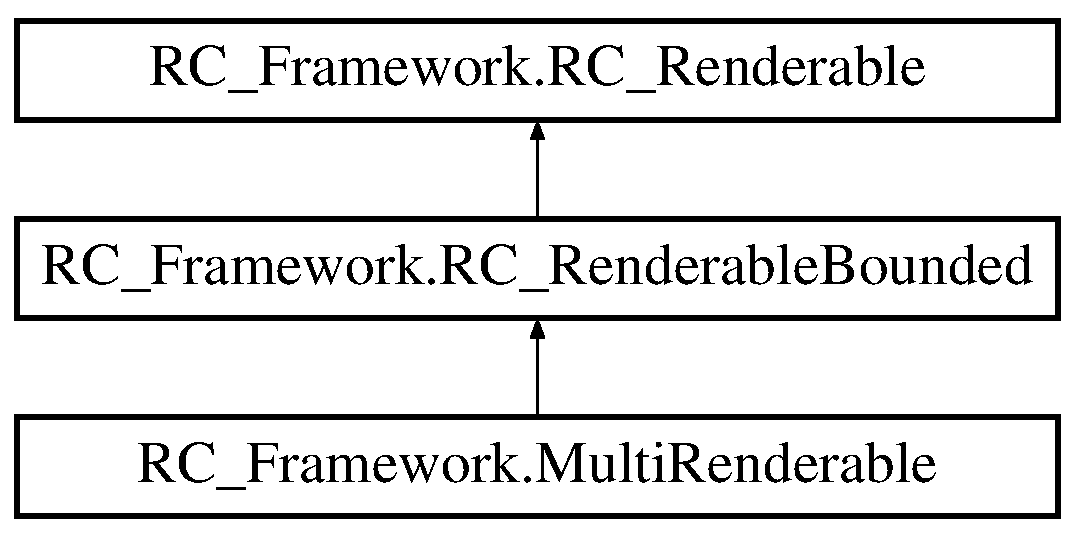
\includegraphics[height=3.000000cm]{class_r_c___framework_1_1_multi_renderable}
\end{center}
\end{figure}
\subsection*{Public Member Functions}
\begin{DoxyCompactItemize}
\item 
\mbox{\hyperlink{class_r_c___framework_1_1_multi_renderable_a86a299bbcb99c632f2b123a100fa9eef}{Multi\+Renderable}} (Rectangle boundsZ, \mbox{\hyperlink{class_r_c___framework_1_1_r_c___renderable_bounded}{R\+C\+\_\+\+Renderable\+Bounded}} sbb1, \mbox{\hyperlink{class_r_c___framework_1_1_r_c___renderable_bounded}{R\+C\+\_\+\+Renderable\+Bounded}} sbb2, \mbox{\hyperlink{class_r_c___framework_1_1_r_c___renderable_bounded}{R\+C\+\_\+\+Renderable\+Bounded}} sbb3, \mbox{\hyperlink{class_r_c___framework_1_1_r_c___renderable_bounded}{R\+C\+\_\+\+Renderable\+Bounded}} sbb4)
\item 
void \mbox{\hyperlink{class_r_c___framework_1_1_multi_renderable_a923ab24c09b28daaf29c65d14d23b3ff}{set\+Bounds}} (Rectangle boundsZ)
\item 
override void \mbox{\hyperlink{class_r_c___framework_1_1_multi_renderable_a3eabd07384410252141e9b10e52b1783}{Update}} (Game\+Time game\+Time)
\item 
override void \mbox{\hyperlink{class_r_c___framework_1_1_multi_renderable_ae81e6924e30c2ff36c5b13204f3d2857}{Draw}} (Sprite\+Batch sb)
\begin{DoxyCompactList}\small\item\em Standard draw routine which assumes the renderable knows where it is \end{DoxyCompactList}\end{DoxyCompactItemize}
\subsection*{Public Attributes}
\begin{DoxyCompactItemize}
\item 
\mbox{\hyperlink{class_r_c___framework_1_1_r_c___renderable_bounded}{R\+C\+\_\+\+Renderable\+Bounded}} \mbox{\hyperlink{class_r_c___framework_1_1_multi_renderable_a362c7065ca22231b1b4fddc581b839e5}{sb1}} = null
\item 
\mbox{\hyperlink{class_r_c___framework_1_1_r_c___renderable_bounded}{R\+C\+\_\+\+Renderable\+Bounded}} \mbox{\hyperlink{class_r_c___framework_1_1_multi_renderable_af0f44a3fc8d4c18fcadbeac11b9eec17}{sb2}} = null
\item 
\mbox{\hyperlink{class_r_c___framework_1_1_r_c___renderable_bounded}{R\+C\+\_\+\+Renderable\+Bounded}} \mbox{\hyperlink{class_r_c___framework_1_1_multi_renderable_ab8aacac69926e1ac7746ddcfcf32b604}{sb3}} = null
\item 
\mbox{\hyperlink{class_r_c___framework_1_1_r_c___renderable_bounded}{R\+C\+\_\+\+Renderable\+Bounded}} \mbox{\hyperlink{class_r_c___framework_1_1_multi_renderable_a24b67c770fadae584a5d0890f5cef70b}{sb4}} = null
\end{DoxyCompactItemize}
\subsection*{Additional Inherited Members}


\subsection{Detailed Description}
This class is just up to 4 bounded renderables for coalessing renderables to gethr in more usefull ways, (eg paralax backgrounds) 

\subsection{Constructor \& Destructor Documentation}
\mbox{\Hypertarget{class_r_c___framework_1_1_multi_renderable_a86a299bbcb99c632f2b123a100fa9eef}\label{class_r_c___framework_1_1_multi_renderable_a86a299bbcb99c632f2b123a100fa9eef}} 
\index{R\+C\+\_\+\+Framework\+::\+Multi\+Renderable@{R\+C\+\_\+\+Framework\+::\+Multi\+Renderable}!Multi\+Renderable@{Multi\+Renderable}}
\index{Multi\+Renderable@{Multi\+Renderable}!R\+C\+\_\+\+Framework\+::\+Multi\+Renderable@{R\+C\+\_\+\+Framework\+::\+Multi\+Renderable}}
\subsubsection{\texorpdfstring{Multi\+Renderable()}{MultiRenderable()}}
{\footnotesize\ttfamily R\+C\+\_\+\+Framework.\+Multi\+Renderable.\+Multi\+Renderable (\begin{DoxyParamCaption}\item[{Rectangle}]{boundsZ,  }\item[{\mbox{\hyperlink{class_r_c___framework_1_1_r_c___renderable_bounded}{R\+C\+\_\+\+Renderable\+Bounded}}}]{sbb1,  }\item[{\mbox{\hyperlink{class_r_c___framework_1_1_r_c___renderable_bounded}{R\+C\+\_\+\+Renderable\+Bounded}}}]{sbb2,  }\item[{\mbox{\hyperlink{class_r_c___framework_1_1_r_c___renderable_bounded}{R\+C\+\_\+\+Renderable\+Bounded}}}]{sbb3,  }\item[{\mbox{\hyperlink{class_r_c___framework_1_1_r_c___renderable_bounded}{R\+C\+\_\+\+Renderable\+Bounded}}}]{sbb4 }\end{DoxyParamCaption})}



\subsection{Member Function Documentation}
\mbox{\Hypertarget{class_r_c___framework_1_1_multi_renderable_ae81e6924e30c2ff36c5b13204f3d2857}\label{class_r_c___framework_1_1_multi_renderable_ae81e6924e30c2ff36c5b13204f3d2857}} 
\index{R\+C\+\_\+\+Framework\+::\+Multi\+Renderable@{R\+C\+\_\+\+Framework\+::\+Multi\+Renderable}!Draw@{Draw}}
\index{Draw@{Draw}!R\+C\+\_\+\+Framework\+::\+Multi\+Renderable@{R\+C\+\_\+\+Framework\+::\+Multi\+Renderable}}
\subsubsection{\texorpdfstring{Draw()}{Draw()}}
{\footnotesize\ttfamily override void R\+C\+\_\+\+Framework.\+Multi\+Renderable.\+Draw (\begin{DoxyParamCaption}\item[{Sprite\+Batch}]{sb }\end{DoxyParamCaption})\hspace{0.3cm}{\ttfamily [virtual]}}



Standard draw routine which assumes the renderable knows where it is 


\begin{DoxyParams}{Parameters}
{\em sb} & \\
\hline
\end{DoxyParams}


Reimplemented from \mbox{\hyperlink{class_r_c___framework_1_1_r_c___renderable_acc26db34e382a25a989c4c0dd0354b23}{R\+C\+\_\+\+Framework.\+R\+C\+\_\+\+Renderable}}.

\mbox{\Hypertarget{class_r_c___framework_1_1_multi_renderable_a923ab24c09b28daaf29c65d14d23b3ff}\label{class_r_c___framework_1_1_multi_renderable_a923ab24c09b28daaf29c65d14d23b3ff}} 
\index{R\+C\+\_\+\+Framework\+::\+Multi\+Renderable@{R\+C\+\_\+\+Framework\+::\+Multi\+Renderable}!set\+Bounds@{set\+Bounds}}
\index{set\+Bounds@{set\+Bounds}!R\+C\+\_\+\+Framework\+::\+Multi\+Renderable@{R\+C\+\_\+\+Framework\+::\+Multi\+Renderable}}
\subsubsection{\texorpdfstring{set\+Bounds()}{setBounds()}}
{\footnotesize\ttfamily void R\+C\+\_\+\+Framework.\+Multi\+Renderable.\+set\+Bounds (\begin{DoxyParamCaption}\item[{Rectangle}]{boundsZ }\end{DoxyParamCaption})}

\mbox{\Hypertarget{class_r_c___framework_1_1_multi_renderable_a3eabd07384410252141e9b10e52b1783}\label{class_r_c___framework_1_1_multi_renderable_a3eabd07384410252141e9b10e52b1783}} 
\index{R\+C\+\_\+\+Framework\+::\+Multi\+Renderable@{R\+C\+\_\+\+Framework\+::\+Multi\+Renderable}!Update@{Update}}
\index{Update@{Update}!R\+C\+\_\+\+Framework\+::\+Multi\+Renderable@{R\+C\+\_\+\+Framework\+::\+Multi\+Renderable}}
\subsubsection{\texorpdfstring{Update()}{Update()}}
{\footnotesize\ttfamily override void R\+C\+\_\+\+Framework.\+Multi\+Renderable.\+Update (\begin{DoxyParamCaption}\item[{Game\+Time}]{game\+Time }\end{DoxyParamCaption})\hspace{0.3cm}{\ttfamily [virtual]}}



Reimplemented from \mbox{\hyperlink{class_r_c___framework_1_1_r_c___renderable_a5745bedc7ba0587aa1e1d8563c357228}{R\+C\+\_\+\+Framework.\+R\+C\+\_\+\+Renderable}}.



\subsection{Member Data Documentation}
\mbox{\Hypertarget{class_r_c___framework_1_1_multi_renderable_a362c7065ca22231b1b4fddc581b839e5}\label{class_r_c___framework_1_1_multi_renderable_a362c7065ca22231b1b4fddc581b839e5}} 
\index{R\+C\+\_\+\+Framework\+::\+Multi\+Renderable@{R\+C\+\_\+\+Framework\+::\+Multi\+Renderable}!sb1@{sb1}}
\index{sb1@{sb1}!R\+C\+\_\+\+Framework\+::\+Multi\+Renderable@{R\+C\+\_\+\+Framework\+::\+Multi\+Renderable}}
\subsubsection{\texorpdfstring{sb1}{sb1}}
{\footnotesize\ttfamily \mbox{\hyperlink{class_r_c___framework_1_1_r_c___renderable_bounded}{R\+C\+\_\+\+Renderable\+Bounded}} R\+C\+\_\+\+Framework.\+Multi\+Renderable.\+sb1 = null}

\mbox{\Hypertarget{class_r_c___framework_1_1_multi_renderable_af0f44a3fc8d4c18fcadbeac11b9eec17}\label{class_r_c___framework_1_1_multi_renderable_af0f44a3fc8d4c18fcadbeac11b9eec17}} 
\index{R\+C\+\_\+\+Framework\+::\+Multi\+Renderable@{R\+C\+\_\+\+Framework\+::\+Multi\+Renderable}!sb2@{sb2}}
\index{sb2@{sb2}!R\+C\+\_\+\+Framework\+::\+Multi\+Renderable@{R\+C\+\_\+\+Framework\+::\+Multi\+Renderable}}
\subsubsection{\texorpdfstring{sb2}{sb2}}
{\footnotesize\ttfamily \mbox{\hyperlink{class_r_c___framework_1_1_r_c___renderable_bounded}{R\+C\+\_\+\+Renderable\+Bounded}} R\+C\+\_\+\+Framework.\+Multi\+Renderable.\+sb2 = null}

\mbox{\Hypertarget{class_r_c___framework_1_1_multi_renderable_ab8aacac69926e1ac7746ddcfcf32b604}\label{class_r_c___framework_1_1_multi_renderable_ab8aacac69926e1ac7746ddcfcf32b604}} 
\index{R\+C\+\_\+\+Framework\+::\+Multi\+Renderable@{R\+C\+\_\+\+Framework\+::\+Multi\+Renderable}!sb3@{sb3}}
\index{sb3@{sb3}!R\+C\+\_\+\+Framework\+::\+Multi\+Renderable@{R\+C\+\_\+\+Framework\+::\+Multi\+Renderable}}
\subsubsection{\texorpdfstring{sb3}{sb3}}
{\footnotesize\ttfamily \mbox{\hyperlink{class_r_c___framework_1_1_r_c___renderable_bounded}{R\+C\+\_\+\+Renderable\+Bounded}} R\+C\+\_\+\+Framework.\+Multi\+Renderable.\+sb3 = null}

\mbox{\Hypertarget{class_r_c___framework_1_1_multi_renderable_a24b67c770fadae584a5d0890f5cef70b}\label{class_r_c___framework_1_1_multi_renderable_a24b67c770fadae584a5d0890f5cef70b}} 
\index{R\+C\+\_\+\+Framework\+::\+Multi\+Renderable@{R\+C\+\_\+\+Framework\+::\+Multi\+Renderable}!sb4@{sb4}}
\index{sb4@{sb4}!R\+C\+\_\+\+Framework\+::\+Multi\+Renderable@{R\+C\+\_\+\+Framework\+::\+Multi\+Renderable}}
\subsubsection{\texorpdfstring{sb4}{sb4}}
{\footnotesize\ttfamily \mbox{\hyperlink{class_r_c___framework_1_1_r_c___renderable_bounded}{R\+C\+\_\+\+Renderable\+Bounded}} R\+C\+\_\+\+Framework.\+Multi\+Renderable.\+sb4 = null}



The documentation for this class was generated from the following file\+:\begin{DoxyCompactItemize}
\item 
F\+:/\+B/\+R\+C\+\_\+\+Framework2018/\+Source/\mbox{\hyperlink{_r_c___renderable_multi_8cs}{R\+C\+\_\+\+Renderable\+Multi.\+cs}}\end{DoxyCompactItemize}

\hypertarget{class_r_c___framework_1_1_multi_scroll_back_ground}{}\section{R\+C\+\_\+\+Framework.\+Multi\+Scroll\+Back\+Ground Class Reference}
\label{class_r_c___framework_1_1_multi_scroll_back_ground}\index{R\+C\+\_\+\+Framework.\+Multi\+Scroll\+Back\+Ground@{R\+C\+\_\+\+Framework.\+Multi\+Scroll\+Back\+Ground}}
Inheritance diagram for R\+C\+\_\+\+Framework.\+Multi\+Scroll\+Back\+Ground\+:\begin{figure}[H]
\begin{center}
\leavevmode
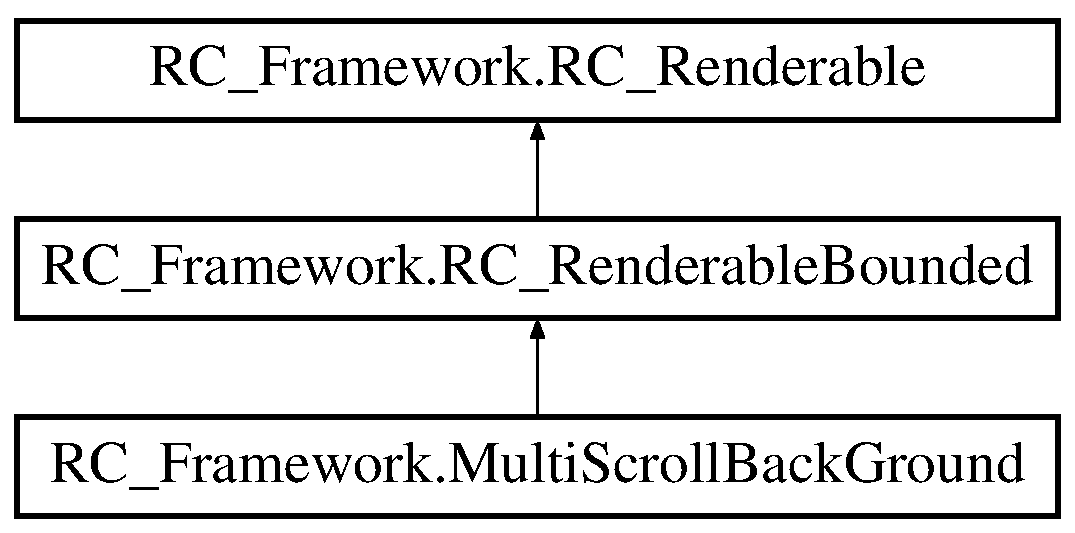
\includegraphics[height=3.000000cm]{class_r_c___framework_1_1_multi_scroll_back_ground}
\end{center}
\end{figure}
\subsection*{Public Member Functions}
\begin{DoxyCompactItemize}
\item 
\mbox{\hyperlink{class_r_c___framework_1_1_multi_scroll_back_ground_a080400ff40d4fb293197930c6a76560e}{Multi\+Scroll\+Back\+Ground}} (Rectangle boundsZ)
\item 
void \mbox{\hyperlink{class_r_c___framework_1_1_multi_scroll_back_ground_a480037cbf0141cd66686b3692f1af978}{set\+Scroll\+Back\+Grounds}} (\mbox{\hyperlink{class_r_c___framework_1_1_scroll_back_ground}{Scroll\+Back\+Ground}} sbb1, \mbox{\hyperlink{class_r_c___framework_1_1_scroll_back_ground}{Scroll\+Back\+Ground}} sbb2, \mbox{\hyperlink{class_r_c___framework_1_1_scroll_back_ground}{Scroll\+Back\+Ground}} sbb3)
\item 
override void \mbox{\hyperlink{class_r_c___framework_1_1_multi_scroll_back_ground_aed0cdef9bd5f161cde89af98dcf63e24}{Update}} (Game\+Time game\+Time)
\item 
override void \mbox{\hyperlink{class_r_c___framework_1_1_multi_scroll_back_ground_ac59e7e1e7a2e1ccfc364883b98765f00}{Draw}} (Sprite\+Batch sb)
\begin{DoxyCompactList}\small\item\em Standard draw routine which assumes the renderable knows where it is \end{DoxyCompactList}\end{DoxyCompactItemize}
\subsection*{Public Attributes}
\begin{DoxyCompactItemize}
\item 
\mbox{\hyperlink{class_r_c___framework_1_1_scroll_back_ground}{Scroll\+Back\+Ground}} \mbox{\hyperlink{class_r_c___framework_1_1_multi_scroll_back_ground_a20cc204c6f10652592dc1429e20d3a1e}{sb1}} = null
\item 
\mbox{\hyperlink{class_r_c___framework_1_1_scroll_back_ground}{Scroll\+Back\+Ground}} \mbox{\hyperlink{class_r_c___framework_1_1_multi_scroll_back_ground_a3d2a684350de4c4fbc262248cc6b8aff}{sb2}} = null
\item 
\mbox{\hyperlink{class_r_c___framework_1_1_scroll_back_ground}{Scroll\+Back\+Ground}} \mbox{\hyperlink{class_r_c___framework_1_1_multi_scroll_back_ground_ae010d29cb2cf4bd24b459679a37cd7a4}{sb3}} = null
\end{DoxyCompactItemize}
\subsection*{Additional Inherited Members}


\subsection{Constructor \& Destructor Documentation}
\mbox{\Hypertarget{class_r_c___framework_1_1_multi_scroll_back_ground_a080400ff40d4fb293197930c6a76560e}\label{class_r_c___framework_1_1_multi_scroll_back_ground_a080400ff40d4fb293197930c6a76560e}} 
\index{R\+C\+\_\+\+Framework\+::\+Multi\+Scroll\+Back\+Ground@{R\+C\+\_\+\+Framework\+::\+Multi\+Scroll\+Back\+Ground}!Multi\+Scroll\+Back\+Ground@{Multi\+Scroll\+Back\+Ground}}
\index{Multi\+Scroll\+Back\+Ground@{Multi\+Scroll\+Back\+Ground}!R\+C\+\_\+\+Framework\+::\+Multi\+Scroll\+Back\+Ground@{R\+C\+\_\+\+Framework\+::\+Multi\+Scroll\+Back\+Ground}}
\subsubsection{\texorpdfstring{Multi\+Scroll\+Back\+Ground()}{MultiScrollBackGround()}}
{\footnotesize\ttfamily R\+C\+\_\+\+Framework.\+Multi\+Scroll\+Back\+Ground.\+Multi\+Scroll\+Back\+Ground (\begin{DoxyParamCaption}\item[{Rectangle}]{boundsZ }\end{DoxyParamCaption})}



\subsection{Member Function Documentation}
\mbox{\Hypertarget{class_r_c___framework_1_1_multi_scroll_back_ground_ac59e7e1e7a2e1ccfc364883b98765f00}\label{class_r_c___framework_1_1_multi_scroll_back_ground_ac59e7e1e7a2e1ccfc364883b98765f00}} 
\index{R\+C\+\_\+\+Framework\+::\+Multi\+Scroll\+Back\+Ground@{R\+C\+\_\+\+Framework\+::\+Multi\+Scroll\+Back\+Ground}!Draw@{Draw}}
\index{Draw@{Draw}!R\+C\+\_\+\+Framework\+::\+Multi\+Scroll\+Back\+Ground@{R\+C\+\_\+\+Framework\+::\+Multi\+Scroll\+Back\+Ground}}
\subsubsection{\texorpdfstring{Draw()}{Draw()}}
{\footnotesize\ttfamily override void R\+C\+\_\+\+Framework.\+Multi\+Scroll\+Back\+Ground.\+Draw (\begin{DoxyParamCaption}\item[{Sprite\+Batch}]{sb }\end{DoxyParamCaption})\hspace{0.3cm}{\ttfamily [virtual]}}



Standard draw routine which assumes the renderable knows where it is 


\begin{DoxyParams}{Parameters}
{\em sb} & \\
\hline
\end{DoxyParams}


Reimplemented from \mbox{\hyperlink{class_r_c___framework_1_1_r_c___renderable_acc26db34e382a25a989c4c0dd0354b23}{R\+C\+\_\+\+Framework.\+R\+C\+\_\+\+Renderable}}.

\mbox{\Hypertarget{class_r_c___framework_1_1_multi_scroll_back_ground_a480037cbf0141cd66686b3692f1af978}\label{class_r_c___framework_1_1_multi_scroll_back_ground_a480037cbf0141cd66686b3692f1af978}} 
\index{R\+C\+\_\+\+Framework\+::\+Multi\+Scroll\+Back\+Ground@{R\+C\+\_\+\+Framework\+::\+Multi\+Scroll\+Back\+Ground}!set\+Scroll\+Back\+Grounds@{set\+Scroll\+Back\+Grounds}}
\index{set\+Scroll\+Back\+Grounds@{set\+Scroll\+Back\+Grounds}!R\+C\+\_\+\+Framework\+::\+Multi\+Scroll\+Back\+Ground@{R\+C\+\_\+\+Framework\+::\+Multi\+Scroll\+Back\+Ground}}
\subsubsection{\texorpdfstring{set\+Scroll\+Back\+Grounds()}{setScrollBackGrounds()}}
{\footnotesize\ttfamily void R\+C\+\_\+\+Framework.\+Multi\+Scroll\+Back\+Ground.\+set\+Scroll\+Back\+Grounds (\begin{DoxyParamCaption}\item[{\mbox{\hyperlink{class_r_c___framework_1_1_scroll_back_ground}{Scroll\+Back\+Ground}}}]{sbb1,  }\item[{\mbox{\hyperlink{class_r_c___framework_1_1_scroll_back_ground}{Scroll\+Back\+Ground}}}]{sbb2,  }\item[{\mbox{\hyperlink{class_r_c___framework_1_1_scroll_back_ground}{Scroll\+Back\+Ground}}}]{sbb3 }\end{DoxyParamCaption})}

\mbox{\Hypertarget{class_r_c___framework_1_1_multi_scroll_back_ground_aed0cdef9bd5f161cde89af98dcf63e24}\label{class_r_c___framework_1_1_multi_scroll_back_ground_aed0cdef9bd5f161cde89af98dcf63e24}} 
\index{R\+C\+\_\+\+Framework\+::\+Multi\+Scroll\+Back\+Ground@{R\+C\+\_\+\+Framework\+::\+Multi\+Scroll\+Back\+Ground}!Update@{Update}}
\index{Update@{Update}!R\+C\+\_\+\+Framework\+::\+Multi\+Scroll\+Back\+Ground@{R\+C\+\_\+\+Framework\+::\+Multi\+Scroll\+Back\+Ground}}
\subsubsection{\texorpdfstring{Update()}{Update()}}
{\footnotesize\ttfamily override void R\+C\+\_\+\+Framework.\+Multi\+Scroll\+Back\+Ground.\+Update (\begin{DoxyParamCaption}\item[{Game\+Time}]{game\+Time }\end{DoxyParamCaption})\hspace{0.3cm}{\ttfamily [virtual]}}



Reimplemented from \mbox{\hyperlink{class_r_c___framework_1_1_r_c___renderable_a5745bedc7ba0587aa1e1d8563c357228}{R\+C\+\_\+\+Framework.\+R\+C\+\_\+\+Renderable}}.



\subsection{Member Data Documentation}
\mbox{\Hypertarget{class_r_c___framework_1_1_multi_scroll_back_ground_a20cc204c6f10652592dc1429e20d3a1e}\label{class_r_c___framework_1_1_multi_scroll_back_ground_a20cc204c6f10652592dc1429e20d3a1e}} 
\index{R\+C\+\_\+\+Framework\+::\+Multi\+Scroll\+Back\+Ground@{R\+C\+\_\+\+Framework\+::\+Multi\+Scroll\+Back\+Ground}!sb1@{sb1}}
\index{sb1@{sb1}!R\+C\+\_\+\+Framework\+::\+Multi\+Scroll\+Back\+Ground@{R\+C\+\_\+\+Framework\+::\+Multi\+Scroll\+Back\+Ground}}
\subsubsection{\texorpdfstring{sb1}{sb1}}
{\footnotesize\ttfamily \mbox{\hyperlink{class_r_c___framework_1_1_scroll_back_ground}{Scroll\+Back\+Ground}} R\+C\+\_\+\+Framework.\+Multi\+Scroll\+Back\+Ground.\+sb1 = null}

\mbox{\Hypertarget{class_r_c___framework_1_1_multi_scroll_back_ground_a3d2a684350de4c4fbc262248cc6b8aff}\label{class_r_c___framework_1_1_multi_scroll_back_ground_a3d2a684350de4c4fbc262248cc6b8aff}} 
\index{R\+C\+\_\+\+Framework\+::\+Multi\+Scroll\+Back\+Ground@{R\+C\+\_\+\+Framework\+::\+Multi\+Scroll\+Back\+Ground}!sb2@{sb2}}
\index{sb2@{sb2}!R\+C\+\_\+\+Framework\+::\+Multi\+Scroll\+Back\+Ground@{R\+C\+\_\+\+Framework\+::\+Multi\+Scroll\+Back\+Ground}}
\subsubsection{\texorpdfstring{sb2}{sb2}}
{\footnotesize\ttfamily \mbox{\hyperlink{class_r_c___framework_1_1_scroll_back_ground}{Scroll\+Back\+Ground}} R\+C\+\_\+\+Framework.\+Multi\+Scroll\+Back\+Ground.\+sb2 = null}

\mbox{\Hypertarget{class_r_c___framework_1_1_multi_scroll_back_ground_ae010d29cb2cf4bd24b459679a37cd7a4}\label{class_r_c___framework_1_1_multi_scroll_back_ground_ae010d29cb2cf4bd24b459679a37cd7a4}} 
\index{R\+C\+\_\+\+Framework\+::\+Multi\+Scroll\+Back\+Ground@{R\+C\+\_\+\+Framework\+::\+Multi\+Scroll\+Back\+Ground}!sb3@{sb3}}
\index{sb3@{sb3}!R\+C\+\_\+\+Framework\+::\+Multi\+Scroll\+Back\+Ground@{R\+C\+\_\+\+Framework\+::\+Multi\+Scroll\+Back\+Ground}}
\subsubsection{\texorpdfstring{sb3}{sb3}}
{\footnotesize\ttfamily \mbox{\hyperlink{class_r_c___framework_1_1_scroll_back_ground}{Scroll\+Back\+Ground}} R\+C\+\_\+\+Framework.\+Multi\+Scroll\+Back\+Ground.\+sb3 = null}



The documentation for this class was generated from the following file\+:\begin{DoxyCompactItemize}
\item 
F\+:/\+B/\+R\+C\+\_\+\+Framework2018/\+Source/\mbox{\hyperlink{_r_c___renderable_multi_8cs}{R\+C\+\_\+\+Renderable\+Multi.\+cs}}\end{DoxyCompactItemize}

\hypertarget{class_r_c___framework_1_1_pan_zoom_sequence}{}\section{R\+C\+\_\+\+Framework.\+Pan\+Zoom\+Sequence Class Reference}
\label{class_r_c___framework_1_1_pan_zoom_sequence}\index{R\+C\+\_\+\+Framework.\+Pan\+Zoom\+Sequence@{R\+C\+\_\+\+Framework.\+Pan\+Zoom\+Sequence}}
Inheritance diagram for R\+C\+\_\+\+Framework.\+Pan\+Zoom\+Sequence\+:\begin{figure}[H]
\begin{center}
\leavevmode
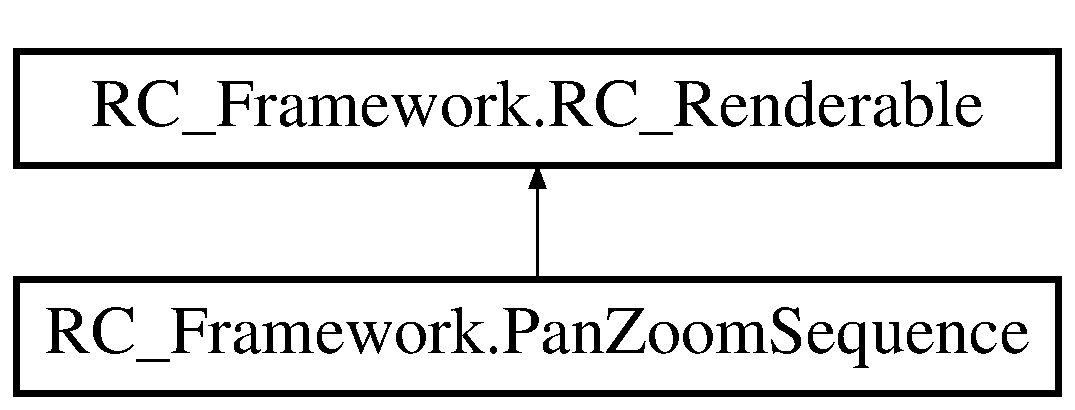
\includegraphics[height=2.000000cm]{class_r_c___framework_1_1_pan_zoom_sequence}
\end{center}
\end{figure}
\subsection*{Public Member Functions}
\begin{DoxyCompactItemize}
\item 
\mbox{\hyperlink{class_r_c___framework_1_1_pan_zoom_sequence_acf6051001df62fee79c67a3e53012341}{Pan\+Zoom\+Sequence}} (Rectangle destZ, Texture2D default\+TexZ, Color default\+ColorZ)
\item 
override void \mbox{\hyperlink{class_r_c___framework_1_1_pan_zoom_sequence_ab235ec7298062b4e3a028979c5abad5c}{reset}} ()
\item 
void \mbox{\hyperlink{class_r_c___framework_1_1_pan_zoom_sequence_a6e2a1cbdd12386dd59daab6ab1bb94fc}{add\+Stage}} (\mbox{\hyperlink{class_r_c___framework_1_1_pan_zoom_stage}{Pan\+Zoom\+Stage}} s)
\item 
void \mbox{\hyperlink{class_r_c___framework_1_1_pan_zoom_sequence_a35676939d35ab90a9a8c855a9fcf4479}{add\+Stage}} (Texture2D texZ, int ticks\+To\+TransitZ, Color init\+ColourZ, Color final\+ColourZ, Rectangle init\+DestZ, Rectangle final\+DestZ, Rectangle init\+SourceZ, Rectangle final\+SourceZ)
\item 
void \mbox{\hyperlink{class_r_c___framework_1_1_pan_zoom_sequence_ac8daade410a23e40a6050b0152d28cf9}{add\+Stage}} (int ticks\+To\+TransitZ, Rectangle init\+SourceZ)
\item 
void \mbox{\hyperlink{class_r_c___framework_1_1_pan_zoom_sequence_a5ac14ab5b1b52c28349481afb6f4b8b5}{add\+Stage}} (int ticks\+To\+TransitZ, Rectangle init\+SourceZ, Rectangle final\+SourceZ)
\item 
bool \mbox{\hyperlink{class_r_c___framework_1_1_pan_zoom_sequence_a7e24734bce4072f60e65cc1b63ca460c}{Done}} ()
\item 
override void \mbox{\hyperlink{class_r_c___framework_1_1_pan_zoom_sequence_a1c15ccaf96c79adece0f665f1419f95b}{Update}} (Game\+Time game\+Time)
\item 
override void \mbox{\hyperlink{class_r_c___framework_1_1_pan_zoom_sequence_a63516b58108ff5f5bcb03d24230128f3}{Draw}} (Sprite\+Batch sb)
\begin{DoxyCompactList}\small\item\em Standard draw routine which assumes the renderable knows where it is \end{DoxyCompactList}\end{DoxyCompactItemize}
\subsection*{Public Attributes}
\begin{DoxyCompactItemize}
\item 
List$<$ \mbox{\hyperlink{class_r_c___framework_1_1_pan_zoom_stage}{Pan\+Zoom\+Stage}} $>$ \mbox{\hyperlink{class_r_c___framework_1_1_pan_zoom_sequence_ae20aeed249f040a8f132657fae2087ec}{lst}}
\end{DoxyCompactItemize}
\subsection*{Properties}
\begin{DoxyCompactItemize}
\item 
Texture2D \mbox{\hyperlink{class_r_c___framework_1_1_pan_zoom_sequence_a39a1630167632f8cfd7004083f9f8099}{default\+Tex}}\hspace{0.3cm}{\ttfamily  \mbox{[}get, set\mbox{]}}
\item 
Rectangle \mbox{\hyperlink{class_r_c___framework_1_1_pan_zoom_sequence_ab3b02fbe31f614dc4e7fdc5d3ff076d0}{default\+Dest}}\hspace{0.3cm}{\ttfamily  \mbox{[}get, set\mbox{]}}
\item 
Color \mbox{\hyperlink{class_r_c___framework_1_1_pan_zoom_sequence_a252b67cb0eb86c4dd81ce80230421ca5}{default\+Colour}}\hspace{0.3cm}{\ttfamily  \mbox{[}get, set\mbox{]}}
\end{DoxyCompactItemize}


\subsection{Constructor \& Destructor Documentation}
\mbox{\Hypertarget{class_r_c___framework_1_1_pan_zoom_sequence_acf6051001df62fee79c67a3e53012341}\label{class_r_c___framework_1_1_pan_zoom_sequence_acf6051001df62fee79c67a3e53012341}} 
\index{R\+C\+\_\+\+Framework\+::\+Pan\+Zoom\+Sequence@{R\+C\+\_\+\+Framework\+::\+Pan\+Zoom\+Sequence}!Pan\+Zoom\+Sequence@{Pan\+Zoom\+Sequence}}
\index{Pan\+Zoom\+Sequence@{Pan\+Zoom\+Sequence}!R\+C\+\_\+\+Framework\+::\+Pan\+Zoom\+Sequence@{R\+C\+\_\+\+Framework\+::\+Pan\+Zoom\+Sequence}}
\subsubsection{\texorpdfstring{Pan\+Zoom\+Sequence()}{PanZoomSequence()}}
{\footnotesize\ttfamily R\+C\+\_\+\+Framework.\+Pan\+Zoom\+Sequence.\+Pan\+Zoom\+Sequence (\begin{DoxyParamCaption}\item[{Rectangle}]{destZ,  }\item[{Texture2D}]{default\+TexZ,  }\item[{Color}]{default\+ColorZ }\end{DoxyParamCaption})}



\subsection{Member Function Documentation}
\mbox{\Hypertarget{class_r_c___framework_1_1_pan_zoom_sequence_a6e2a1cbdd12386dd59daab6ab1bb94fc}\label{class_r_c___framework_1_1_pan_zoom_sequence_a6e2a1cbdd12386dd59daab6ab1bb94fc}} 
\index{R\+C\+\_\+\+Framework\+::\+Pan\+Zoom\+Sequence@{R\+C\+\_\+\+Framework\+::\+Pan\+Zoom\+Sequence}!add\+Stage@{add\+Stage}}
\index{add\+Stage@{add\+Stage}!R\+C\+\_\+\+Framework\+::\+Pan\+Zoom\+Sequence@{R\+C\+\_\+\+Framework\+::\+Pan\+Zoom\+Sequence}}
\subsubsection{\texorpdfstring{add\+Stage()}{addStage()}\hspace{0.1cm}{\footnotesize\ttfamily [1/4]}}
{\footnotesize\ttfamily void R\+C\+\_\+\+Framework.\+Pan\+Zoom\+Sequence.\+add\+Stage (\begin{DoxyParamCaption}\item[{\mbox{\hyperlink{class_r_c___framework_1_1_pan_zoom_stage}{Pan\+Zoom\+Stage}}}]{s }\end{DoxyParamCaption})}

\mbox{\Hypertarget{class_r_c___framework_1_1_pan_zoom_sequence_a35676939d35ab90a9a8c855a9fcf4479}\label{class_r_c___framework_1_1_pan_zoom_sequence_a35676939d35ab90a9a8c855a9fcf4479}} 
\index{R\+C\+\_\+\+Framework\+::\+Pan\+Zoom\+Sequence@{R\+C\+\_\+\+Framework\+::\+Pan\+Zoom\+Sequence}!add\+Stage@{add\+Stage}}
\index{add\+Stage@{add\+Stage}!R\+C\+\_\+\+Framework\+::\+Pan\+Zoom\+Sequence@{R\+C\+\_\+\+Framework\+::\+Pan\+Zoom\+Sequence}}
\subsubsection{\texorpdfstring{add\+Stage()}{addStage()}\hspace{0.1cm}{\footnotesize\ttfamily [2/4]}}
{\footnotesize\ttfamily void R\+C\+\_\+\+Framework.\+Pan\+Zoom\+Sequence.\+add\+Stage (\begin{DoxyParamCaption}\item[{Texture2D}]{texZ,  }\item[{int}]{ticks\+To\+TransitZ,  }\item[{Color}]{init\+ColourZ,  }\item[{Color}]{final\+ColourZ,  }\item[{Rectangle}]{init\+DestZ,  }\item[{Rectangle}]{final\+DestZ,  }\item[{Rectangle}]{init\+SourceZ,  }\item[{Rectangle}]{final\+SourceZ }\end{DoxyParamCaption})}

\mbox{\Hypertarget{class_r_c___framework_1_1_pan_zoom_sequence_ac8daade410a23e40a6050b0152d28cf9}\label{class_r_c___framework_1_1_pan_zoom_sequence_ac8daade410a23e40a6050b0152d28cf9}} 
\index{R\+C\+\_\+\+Framework\+::\+Pan\+Zoom\+Sequence@{R\+C\+\_\+\+Framework\+::\+Pan\+Zoom\+Sequence}!add\+Stage@{add\+Stage}}
\index{add\+Stage@{add\+Stage}!R\+C\+\_\+\+Framework\+::\+Pan\+Zoom\+Sequence@{R\+C\+\_\+\+Framework\+::\+Pan\+Zoom\+Sequence}}
\subsubsection{\texorpdfstring{add\+Stage()}{addStage()}\hspace{0.1cm}{\footnotesize\ttfamily [3/4]}}
{\footnotesize\ttfamily void R\+C\+\_\+\+Framework.\+Pan\+Zoom\+Sequence.\+add\+Stage (\begin{DoxyParamCaption}\item[{int}]{ticks\+To\+TransitZ,  }\item[{Rectangle}]{init\+SourceZ }\end{DoxyParamCaption})}

\mbox{\Hypertarget{class_r_c___framework_1_1_pan_zoom_sequence_a5ac14ab5b1b52c28349481afb6f4b8b5}\label{class_r_c___framework_1_1_pan_zoom_sequence_a5ac14ab5b1b52c28349481afb6f4b8b5}} 
\index{R\+C\+\_\+\+Framework\+::\+Pan\+Zoom\+Sequence@{R\+C\+\_\+\+Framework\+::\+Pan\+Zoom\+Sequence}!add\+Stage@{add\+Stage}}
\index{add\+Stage@{add\+Stage}!R\+C\+\_\+\+Framework\+::\+Pan\+Zoom\+Sequence@{R\+C\+\_\+\+Framework\+::\+Pan\+Zoom\+Sequence}}
\subsubsection{\texorpdfstring{add\+Stage()}{addStage()}\hspace{0.1cm}{\footnotesize\ttfamily [4/4]}}
{\footnotesize\ttfamily void R\+C\+\_\+\+Framework.\+Pan\+Zoom\+Sequence.\+add\+Stage (\begin{DoxyParamCaption}\item[{int}]{ticks\+To\+TransitZ,  }\item[{Rectangle}]{init\+SourceZ,  }\item[{Rectangle}]{final\+SourceZ }\end{DoxyParamCaption})}

\mbox{\Hypertarget{class_r_c___framework_1_1_pan_zoom_sequence_a7e24734bce4072f60e65cc1b63ca460c}\label{class_r_c___framework_1_1_pan_zoom_sequence_a7e24734bce4072f60e65cc1b63ca460c}} 
\index{R\+C\+\_\+\+Framework\+::\+Pan\+Zoom\+Sequence@{R\+C\+\_\+\+Framework\+::\+Pan\+Zoom\+Sequence}!Done@{Done}}
\index{Done@{Done}!R\+C\+\_\+\+Framework\+::\+Pan\+Zoom\+Sequence@{R\+C\+\_\+\+Framework\+::\+Pan\+Zoom\+Sequence}}
\subsubsection{\texorpdfstring{Done()}{Done()}}
{\footnotesize\ttfamily bool R\+C\+\_\+\+Framework.\+Pan\+Zoom\+Sequence.\+Done (\begin{DoxyParamCaption}{ }\end{DoxyParamCaption})}

\mbox{\Hypertarget{class_r_c___framework_1_1_pan_zoom_sequence_a63516b58108ff5f5bcb03d24230128f3}\label{class_r_c___framework_1_1_pan_zoom_sequence_a63516b58108ff5f5bcb03d24230128f3}} 
\index{R\+C\+\_\+\+Framework\+::\+Pan\+Zoom\+Sequence@{R\+C\+\_\+\+Framework\+::\+Pan\+Zoom\+Sequence}!Draw@{Draw}}
\index{Draw@{Draw}!R\+C\+\_\+\+Framework\+::\+Pan\+Zoom\+Sequence@{R\+C\+\_\+\+Framework\+::\+Pan\+Zoom\+Sequence}}
\subsubsection{\texorpdfstring{Draw()}{Draw()}}
{\footnotesize\ttfamily override void R\+C\+\_\+\+Framework.\+Pan\+Zoom\+Sequence.\+Draw (\begin{DoxyParamCaption}\item[{Sprite\+Batch}]{sb }\end{DoxyParamCaption})\hspace{0.3cm}{\ttfamily [virtual]}}



Standard draw routine which assumes the renderable knows where it is 


\begin{DoxyParams}{Parameters}
{\em sb} & \\
\hline
\end{DoxyParams}


Reimplemented from \mbox{\hyperlink{class_r_c___framework_1_1_r_c___renderable_acc26db34e382a25a989c4c0dd0354b23}{R\+C\+\_\+\+Framework.\+R\+C\+\_\+\+Renderable}}.

\mbox{\Hypertarget{class_r_c___framework_1_1_pan_zoom_sequence_ab235ec7298062b4e3a028979c5abad5c}\label{class_r_c___framework_1_1_pan_zoom_sequence_ab235ec7298062b4e3a028979c5abad5c}} 
\index{R\+C\+\_\+\+Framework\+::\+Pan\+Zoom\+Sequence@{R\+C\+\_\+\+Framework\+::\+Pan\+Zoom\+Sequence}!reset@{reset}}
\index{reset@{reset}!R\+C\+\_\+\+Framework\+::\+Pan\+Zoom\+Sequence@{R\+C\+\_\+\+Framework\+::\+Pan\+Zoom\+Sequence}}
\subsubsection{\texorpdfstring{reset()}{reset()}}
{\footnotesize\ttfamily override void R\+C\+\_\+\+Framework.\+Pan\+Zoom\+Sequence.\+reset (\begin{DoxyParamCaption}{ }\end{DoxyParamCaption})\hspace{0.3cm}{\ttfamily [virtual]}}



Reimplemented from \mbox{\hyperlink{class_r_c___framework_1_1_r_c___renderable_ae65ce69704d15963789f421b58618b1f}{R\+C\+\_\+\+Framework.\+R\+C\+\_\+\+Renderable}}.

\mbox{\Hypertarget{class_r_c___framework_1_1_pan_zoom_sequence_a1c15ccaf96c79adece0f665f1419f95b}\label{class_r_c___framework_1_1_pan_zoom_sequence_a1c15ccaf96c79adece0f665f1419f95b}} 
\index{R\+C\+\_\+\+Framework\+::\+Pan\+Zoom\+Sequence@{R\+C\+\_\+\+Framework\+::\+Pan\+Zoom\+Sequence}!Update@{Update}}
\index{Update@{Update}!R\+C\+\_\+\+Framework\+::\+Pan\+Zoom\+Sequence@{R\+C\+\_\+\+Framework\+::\+Pan\+Zoom\+Sequence}}
\subsubsection{\texorpdfstring{Update()}{Update()}}
{\footnotesize\ttfamily override void R\+C\+\_\+\+Framework.\+Pan\+Zoom\+Sequence.\+Update (\begin{DoxyParamCaption}\item[{Game\+Time}]{game\+Time }\end{DoxyParamCaption})\hspace{0.3cm}{\ttfamily [virtual]}}



Reimplemented from \mbox{\hyperlink{class_r_c___framework_1_1_r_c___renderable_a5745bedc7ba0587aa1e1d8563c357228}{R\+C\+\_\+\+Framework.\+R\+C\+\_\+\+Renderable}}.



\subsection{Member Data Documentation}
\mbox{\Hypertarget{class_r_c___framework_1_1_pan_zoom_sequence_ae20aeed249f040a8f132657fae2087ec}\label{class_r_c___framework_1_1_pan_zoom_sequence_ae20aeed249f040a8f132657fae2087ec}} 
\index{R\+C\+\_\+\+Framework\+::\+Pan\+Zoom\+Sequence@{R\+C\+\_\+\+Framework\+::\+Pan\+Zoom\+Sequence}!lst@{lst}}
\index{lst@{lst}!R\+C\+\_\+\+Framework\+::\+Pan\+Zoom\+Sequence@{R\+C\+\_\+\+Framework\+::\+Pan\+Zoom\+Sequence}}
\subsubsection{\texorpdfstring{lst}{lst}}
{\footnotesize\ttfamily List$<$\mbox{\hyperlink{class_r_c___framework_1_1_pan_zoom_stage}{Pan\+Zoom\+Stage}}$>$ R\+C\+\_\+\+Framework.\+Pan\+Zoom\+Sequence.\+lst}



\subsection{Property Documentation}
\mbox{\Hypertarget{class_r_c___framework_1_1_pan_zoom_sequence_a252b67cb0eb86c4dd81ce80230421ca5}\label{class_r_c___framework_1_1_pan_zoom_sequence_a252b67cb0eb86c4dd81ce80230421ca5}} 
\index{R\+C\+\_\+\+Framework\+::\+Pan\+Zoom\+Sequence@{R\+C\+\_\+\+Framework\+::\+Pan\+Zoom\+Sequence}!default\+Colour@{default\+Colour}}
\index{default\+Colour@{default\+Colour}!R\+C\+\_\+\+Framework\+::\+Pan\+Zoom\+Sequence@{R\+C\+\_\+\+Framework\+::\+Pan\+Zoom\+Sequence}}
\subsubsection{\texorpdfstring{default\+Colour}{defaultColour}}
{\footnotesize\ttfamily Color R\+C\+\_\+\+Framework.\+Pan\+Zoom\+Sequence.\+default\+Colour\hspace{0.3cm}{\ttfamily [get]}, {\ttfamily [set]}}

\mbox{\Hypertarget{class_r_c___framework_1_1_pan_zoom_sequence_ab3b02fbe31f614dc4e7fdc5d3ff076d0}\label{class_r_c___framework_1_1_pan_zoom_sequence_ab3b02fbe31f614dc4e7fdc5d3ff076d0}} 
\index{R\+C\+\_\+\+Framework\+::\+Pan\+Zoom\+Sequence@{R\+C\+\_\+\+Framework\+::\+Pan\+Zoom\+Sequence}!default\+Dest@{default\+Dest}}
\index{default\+Dest@{default\+Dest}!R\+C\+\_\+\+Framework\+::\+Pan\+Zoom\+Sequence@{R\+C\+\_\+\+Framework\+::\+Pan\+Zoom\+Sequence}}
\subsubsection{\texorpdfstring{default\+Dest}{defaultDest}}
{\footnotesize\ttfamily Rectangle R\+C\+\_\+\+Framework.\+Pan\+Zoom\+Sequence.\+default\+Dest\hspace{0.3cm}{\ttfamily [get]}, {\ttfamily [set]}}

\mbox{\Hypertarget{class_r_c___framework_1_1_pan_zoom_sequence_a39a1630167632f8cfd7004083f9f8099}\label{class_r_c___framework_1_1_pan_zoom_sequence_a39a1630167632f8cfd7004083f9f8099}} 
\index{R\+C\+\_\+\+Framework\+::\+Pan\+Zoom\+Sequence@{R\+C\+\_\+\+Framework\+::\+Pan\+Zoom\+Sequence}!default\+Tex@{default\+Tex}}
\index{default\+Tex@{default\+Tex}!R\+C\+\_\+\+Framework\+::\+Pan\+Zoom\+Sequence@{R\+C\+\_\+\+Framework\+::\+Pan\+Zoom\+Sequence}}
\subsubsection{\texorpdfstring{default\+Tex}{defaultTex}}
{\footnotesize\ttfamily Texture2D R\+C\+\_\+\+Framework.\+Pan\+Zoom\+Sequence.\+default\+Tex\hspace{0.3cm}{\ttfamily [get]}, {\ttfamily [set]}}



The documentation for this class was generated from the following file\+:\begin{DoxyCompactItemize}
\item 
F\+:/\+B/\+R\+C\+\_\+\+Framework2018/\+Source/\mbox{\hyperlink{_r_c___pan_zoom_8cs}{R\+C\+\_\+\+Pan\+Zoom.\+cs}}\end{DoxyCompactItemize}

\hypertarget{class_r_c___framework_1_1_pan_zoom_stage}{}\section{R\+C\+\_\+\+Framework.\+Pan\+Zoom\+Stage Class Reference}
\label{class_r_c___framework_1_1_pan_zoom_stage}\index{R\+C\+\_\+\+Framework.\+Pan\+Zoom\+Stage@{R\+C\+\_\+\+Framework.\+Pan\+Zoom\+Stage}}
Inheritance diagram for R\+C\+\_\+\+Framework.\+Pan\+Zoom\+Stage\+:\begin{figure}[H]
\begin{center}
\leavevmode
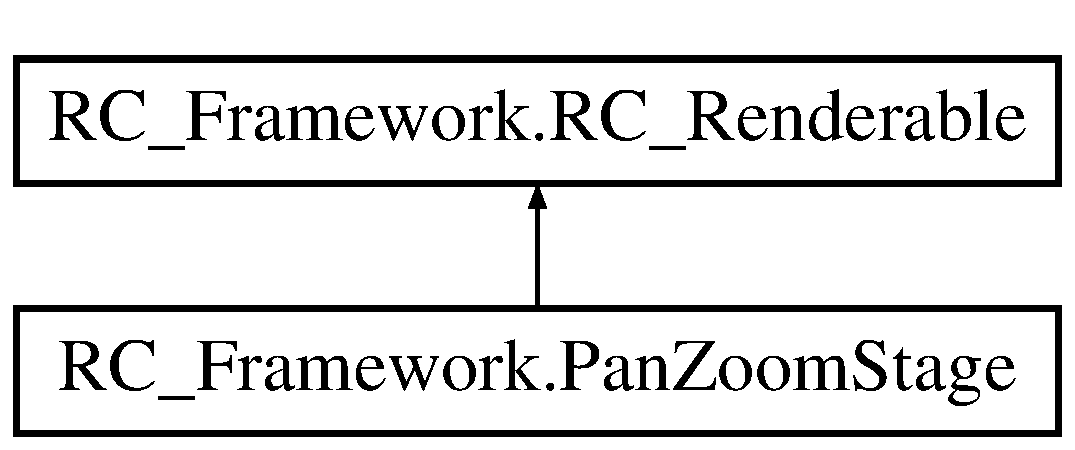
\includegraphics[height=2.000000cm]{class_r_c___framework_1_1_pan_zoom_stage}
\end{center}
\end{figure}
\subsection*{Public Member Functions}
\begin{DoxyCompactItemize}
\item 
\mbox{\hyperlink{class_r_c___framework_1_1_pan_zoom_stage_a2c71701559175b11b3d05c34834d9c18}{Pan\+Zoom\+Stage}} ()
\item 
override void \mbox{\hyperlink{class_r_c___framework_1_1_pan_zoom_stage_a9dc8dc75dab537e608713543ca314284}{reset}} ()
\item 
override void \mbox{\hyperlink{class_r_c___framework_1_1_pan_zoom_stage_a8463539aad705ab51a1ee3b7a64d3f35}{Update}} (Game\+Time game\+Time)
\item 
override void \mbox{\hyperlink{class_r_c___framework_1_1_pan_zoom_stage_a399538cd702d22cb14394f73b1bccff6}{Draw}} (Sprite\+Batch sb)
\begin{DoxyCompactList}\small\item\em Standard draw routine which assumes the renderable knows where it is \end{DoxyCompactList}\end{DoxyCompactItemize}
\subsection*{Properties}
\begin{DoxyCompactItemize}
\item 
Texture2D \mbox{\hyperlink{class_r_c___framework_1_1_pan_zoom_stage_a14a4f47d0ae299d5e0be60d77c97b8f5}{tex}}\hspace{0.3cm}{\ttfamily  \mbox{[}get, set\mbox{]}}
\item 
Rectangle \mbox{\hyperlink{class_r_c___framework_1_1_pan_zoom_stage_ab801249c21a98b50f2a008803dc4931d}{init\+Dest}}\hspace{0.3cm}{\ttfamily  \mbox{[}get, set\mbox{]}}
\item 
Rectangle \mbox{\hyperlink{class_r_c___framework_1_1_pan_zoom_stage_ac50fbe6d15682c9d5c09d59a140a5da1}{final\+Dest}}\hspace{0.3cm}{\ttfamily  \mbox{[}get, set\mbox{]}}
\item 
Rectangle \mbox{\hyperlink{class_r_c___framework_1_1_pan_zoom_stage_ae1b47750162c3793add78db87bc2ded2}{init\+Source}}\hspace{0.3cm}{\ttfamily  \mbox{[}get, set\mbox{]}}
\item 
Rectangle \mbox{\hyperlink{class_r_c___framework_1_1_pan_zoom_stage_a026e22c36ab708eaa1115d3efe9bb707}{final\+Source}}\hspace{0.3cm}{\ttfamily  \mbox{[}get, set\mbox{]}}
\item 
int \mbox{\hyperlink{class_r_c___framework_1_1_pan_zoom_stage_a8377755e226ef4ad9b73fa082eebb569}{ticks\+To\+Transit}}\hspace{0.3cm}{\ttfamily  \mbox{[}get, set\mbox{]}}
\item 
int \mbox{\hyperlink{class_r_c___framework_1_1_pan_zoom_stage_a14dac520d4ea1d613640a30b50e24867}{cnt\+Ticks\+To\+Transit}}\hspace{0.3cm}{\ttfamily  \mbox{[}get, set\mbox{]}}
\item 
Color \mbox{\hyperlink{class_r_c___framework_1_1_pan_zoom_stage_a9a9b17461c43427824ed83a2f2e4527c}{init\+Colour}}\hspace{0.3cm}{\ttfamily  \mbox{[}get, set\mbox{]}}
\item 
Color \mbox{\hyperlink{class_r_c___framework_1_1_pan_zoom_stage_a9d74a8178faeda687f541242dd06025a}{final\+Colour}}\hspace{0.3cm}{\ttfamily  \mbox{[}get, set\mbox{]}}
\item 
bool \mbox{\hyperlink{class_r_c___framework_1_1_pan_zoom_stage_a724e1ef5071cb188af0ee6bee7351769}{done}}\hspace{0.3cm}{\ttfamily  \mbox{[}get, set\mbox{]}}
\end{DoxyCompactItemize}
\subsection*{Additional Inherited Members}


\subsection{Constructor \& Destructor Documentation}
\mbox{\Hypertarget{class_r_c___framework_1_1_pan_zoom_stage_a2c71701559175b11b3d05c34834d9c18}\label{class_r_c___framework_1_1_pan_zoom_stage_a2c71701559175b11b3d05c34834d9c18}} 
\index{R\+C\+\_\+\+Framework\+::\+Pan\+Zoom\+Stage@{R\+C\+\_\+\+Framework\+::\+Pan\+Zoom\+Stage}!Pan\+Zoom\+Stage@{Pan\+Zoom\+Stage}}
\index{Pan\+Zoom\+Stage@{Pan\+Zoom\+Stage}!R\+C\+\_\+\+Framework\+::\+Pan\+Zoom\+Stage@{R\+C\+\_\+\+Framework\+::\+Pan\+Zoom\+Stage}}
\subsubsection{\texorpdfstring{Pan\+Zoom\+Stage()}{PanZoomStage()}}
{\footnotesize\ttfamily R\+C\+\_\+\+Framework.\+Pan\+Zoom\+Stage.\+Pan\+Zoom\+Stage (\begin{DoxyParamCaption}{ }\end{DoxyParamCaption})}



\subsection{Member Function Documentation}
\mbox{\Hypertarget{class_r_c___framework_1_1_pan_zoom_stage_a399538cd702d22cb14394f73b1bccff6}\label{class_r_c___framework_1_1_pan_zoom_stage_a399538cd702d22cb14394f73b1bccff6}} 
\index{R\+C\+\_\+\+Framework\+::\+Pan\+Zoom\+Stage@{R\+C\+\_\+\+Framework\+::\+Pan\+Zoom\+Stage}!Draw@{Draw}}
\index{Draw@{Draw}!R\+C\+\_\+\+Framework\+::\+Pan\+Zoom\+Stage@{R\+C\+\_\+\+Framework\+::\+Pan\+Zoom\+Stage}}
\subsubsection{\texorpdfstring{Draw()}{Draw()}}
{\footnotesize\ttfamily override void R\+C\+\_\+\+Framework.\+Pan\+Zoom\+Stage.\+Draw (\begin{DoxyParamCaption}\item[{Sprite\+Batch}]{sb }\end{DoxyParamCaption})\hspace{0.3cm}{\ttfamily [virtual]}}



Standard draw routine which assumes the renderable knows where it is 


\begin{DoxyParams}{Parameters}
{\em sb} & \\
\hline
\end{DoxyParams}


Reimplemented from \mbox{\hyperlink{class_r_c___framework_1_1_r_c___renderable_acc26db34e382a25a989c4c0dd0354b23}{R\+C\+\_\+\+Framework.\+R\+C\+\_\+\+Renderable}}.

\mbox{\Hypertarget{class_r_c___framework_1_1_pan_zoom_stage_a9dc8dc75dab537e608713543ca314284}\label{class_r_c___framework_1_1_pan_zoom_stage_a9dc8dc75dab537e608713543ca314284}} 
\index{R\+C\+\_\+\+Framework\+::\+Pan\+Zoom\+Stage@{R\+C\+\_\+\+Framework\+::\+Pan\+Zoom\+Stage}!reset@{reset}}
\index{reset@{reset}!R\+C\+\_\+\+Framework\+::\+Pan\+Zoom\+Stage@{R\+C\+\_\+\+Framework\+::\+Pan\+Zoom\+Stage}}
\subsubsection{\texorpdfstring{reset()}{reset()}}
{\footnotesize\ttfamily override void R\+C\+\_\+\+Framework.\+Pan\+Zoom\+Stage.\+reset (\begin{DoxyParamCaption}{ }\end{DoxyParamCaption})\hspace{0.3cm}{\ttfamily [virtual]}}



Reimplemented from \mbox{\hyperlink{class_r_c___framework_1_1_r_c___renderable_ae65ce69704d15963789f421b58618b1f}{R\+C\+\_\+\+Framework.\+R\+C\+\_\+\+Renderable}}.

\mbox{\Hypertarget{class_r_c___framework_1_1_pan_zoom_stage_a8463539aad705ab51a1ee3b7a64d3f35}\label{class_r_c___framework_1_1_pan_zoom_stage_a8463539aad705ab51a1ee3b7a64d3f35}} 
\index{R\+C\+\_\+\+Framework\+::\+Pan\+Zoom\+Stage@{R\+C\+\_\+\+Framework\+::\+Pan\+Zoom\+Stage}!Update@{Update}}
\index{Update@{Update}!R\+C\+\_\+\+Framework\+::\+Pan\+Zoom\+Stage@{R\+C\+\_\+\+Framework\+::\+Pan\+Zoom\+Stage}}
\subsubsection{\texorpdfstring{Update()}{Update()}}
{\footnotesize\ttfamily override void R\+C\+\_\+\+Framework.\+Pan\+Zoom\+Stage.\+Update (\begin{DoxyParamCaption}\item[{Game\+Time}]{game\+Time }\end{DoxyParamCaption})\hspace{0.3cm}{\ttfamily [virtual]}}



Reimplemented from \mbox{\hyperlink{class_r_c___framework_1_1_r_c___renderable_a5745bedc7ba0587aa1e1d8563c357228}{R\+C\+\_\+\+Framework.\+R\+C\+\_\+\+Renderable}}.



\subsection{Property Documentation}
\mbox{\Hypertarget{class_r_c___framework_1_1_pan_zoom_stage_a14dac520d4ea1d613640a30b50e24867}\label{class_r_c___framework_1_1_pan_zoom_stage_a14dac520d4ea1d613640a30b50e24867}} 
\index{R\+C\+\_\+\+Framework\+::\+Pan\+Zoom\+Stage@{R\+C\+\_\+\+Framework\+::\+Pan\+Zoom\+Stage}!cnt\+Ticks\+To\+Transit@{cnt\+Ticks\+To\+Transit}}
\index{cnt\+Ticks\+To\+Transit@{cnt\+Ticks\+To\+Transit}!R\+C\+\_\+\+Framework\+::\+Pan\+Zoom\+Stage@{R\+C\+\_\+\+Framework\+::\+Pan\+Zoom\+Stage}}
\subsubsection{\texorpdfstring{cnt\+Ticks\+To\+Transit}{cntTicksToTransit}}
{\footnotesize\ttfamily int R\+C\+\_\+\+Framework.\+Pan\+Zoom\+Stage.\+cnt\+Ticks\+To\+Transit\hspace{0.3cm}{\ttfamily [get]}, {\ttfamily [set]}}

\mbox{\Hypertarget{class_r_c___framework_1_1_pan_zoom_stage_a724e1ef5071cb188af0ee6bee7351769}\label{class_r_c___framework_1_1_pan_zoom_stage_a724e1ef5071cb188af0ee6bee7351769}} 
\index{R\+C\+\_\+\+Framework\+::\+Pan\+Zoom\+Stage@{R\+C\+\_\+\+Framework\+::\+Pan\+Zoom\+Stage}!done@{done}}
\index{done@{done}!R\+C\+\_\+\+Framework\+::\+Pan\+Zoom\+Stage@{R\+C\+\_\+\+Framework\+::\+Pan\+Zoom\+Stage}}
\subsubsection{\texorpdfstring{done}{done}}
{\footnotesize\ttfamily bool R\+C\+\_\+\+Framework.\+Pan\+Zoom\+Stage.\+done\hspace{0.3cm}{\ttfamily [get]}, {\ttfamily [set]}}

\mbox{\Hypertarget{class_r_c___framework_1_1_pan_zoom_stage_a9d74a8178faeda687f541242dd06025a}\label{class_r_c___framework_1_1_pan_zoom_stage_a9d74a8178faeda687f541242dd06025a}} 
\index{R\+C\+\_\+\+Framework\+::\+Pan\+Zoom\+Stage@{R\+C\+\_\+\+Framework\+::\+Pan\+Zoom\+Stage}!final\+Colour@{final\+Colour}}
\index{final\+Colour@{final\+Colour}!R\+C\+\_\+\+Framework\+::\+Pan\+Zoom\+Stage@{R\+C\+\_\+\+Framework\+::\+Pan\+Zoom\+Stage}}
\subsubsection{\texorpdfstring{final\+Colour}{finalColour}}
{\footnotesize\ttfamily Color R\+C\+\_\+\+Framework.\+Pan\+Zoom\+Stage.\+final\+Colour\hspace{0.3cm}{\ttfamily [get]}, {\ttfamily [set]}}

\mbox{\Hypertarget{class_r_c___framework_1_1_pan_zoom_stage_ac50fbe6d15682c9d5c09d59a140a5da1}\label{class_r_c___framework_1_1_pan_zoom_stage_ac50fbe6d15682c9d5c09d59a140a5da1}} 
\index{R\+C\+\_\+\+Framework\+::\+Pan\+Zoom\+Stage@{R\+C\+\_\+\+Framework\+::\+Pan\+Zoom\+Stage}!final\+Dest@{final\+Dest}}
\index{final\+Dest@{final\+Dest}!R\+C\+\_\+\+Framework\+::\+Pan\+Zoom\+Stage@{R\+C\+\_\+\+Framework\+::\+Pan\+Zoom\+Stage}}
\subsubsection{\texorpdfstring{final\+Dest}{finalDest}}
{\footnotesize\ttfamily Rectangle R\+C\+\_\+\+Framework.\+Pan\+Zoom\+Stage.\+final\+Dest\hspace{0.3cm}{\ttfamily [get]}, {\ttfamily [set]}}

\mbox{\Hypertarget{class_r_c___framework_1_1_pan_zoom_stage_a026e22c36ab708eaa1115d3efe9bb707}\label{class_r_c___framework_1_1_pan_zoom_stage_a026e22c36ab708eaa1115d3efe9bb707}} 
\index{R\+C\+\_\+\+Framework\+::\+Pan\+Zoom\+Stage@{R\+C\+\_\+\+Framework\+::\+Pan\+Zoom\+Stage}!final\+Source@{final\+Source}}
\index{final\+Source@{final\+Source}!R\+C\+\_\+\+Framework\+::\+Pan\+Zoom\+Stage@{R\+C\+\_\+\+Framework\+::\+Pan\+Zoom\+Stage}}
\subsubsection{\texorpdfstring{final\+Source}{finalSource}}
{\footnotesize\ttfamily Rectangle R\+C\+\_\+\+Framework.\+Pan\+Zoom\+Stage.\+final\+Source\hspace{0.3cm}{\ttfamily [get]}, {\ttfamily [set]}}

\mbox{\Hypertarget{class_r_c___framework_1_1_pan_zoom_stage_a9a9b17461c43427824ed83a2f2e4527c}\label{class_r_c___framework_1_1_pan_zoom_stage_a9a9b17461c43427824ed83a2f2e4527c}} 
\index{R\+C\+\_\+\+Framework\+::\+Pan\+Zoom\+Stage@{R\+C\+\_\+\+Framework\+::\+Pan\+Zoom\+Stage}!init\+Colour@{init\+Colour}}
\index{init\+Colour@{init\+Colour}!R\+C\+\_\+\+Framework\+::\+Pan\+Zoom\+Stage@{R\+C\+\_\+\+Framework\+::\+Pan\+Zoom\+Stage}}
\subsubsection{\texorpdfstring{init\+Colour}{initColour}}
{\footnotesize\ttfamily Color R\+C\+\_\+\+Framework.\+Pan\+Zoom\+Stage.\+init\+Colour\hspace{0.3cm}{\ttfamily [get]}, {\ttfamily [set]}}

\mbox{\Hypertarget{class_r_c___framework_1_1_pan_zoom_stage_ab801249c21a98b50f2a008803dc4931d}\label{class_r_c___framework_1_1_pan_zoom_stage_ab801249c21a98b50f2a008803dc4931d}} 
\index{R\+C\+\_\+\+Framework\+::\+Pan\+Zoom\+Stage@{R\+C\+\_\+\+Framework\+::\+Pan\+Zoom\+Stage}!init\+Dest@{init\+Dest}}
\index{init\+Dest@{init\+Dest}!R\+C\+\_\+\+Framework\+::\+Pan\+Zoom\+Stage@{R\+C\+\_\+\+Framework\+::\+Pan\+Zoom\+Stage}}
\subsubsection{\texorpdfstring{init\+Dest}{initDest}}
{\footnotesize\ttfamily Rectangle R\+C\+\_\+\+Framework.\+Pan\+Zoom\+Stage.\+init\+Dest\hspace{0.3cm}{\ttfamily [get]}, {\ttfamily [set]}}

\mbox{\Hypertarget{class_r_c___framework_1_1_pan_zoom_stage_ae1b47750162c3793add78db87bc2ded2}\label{class_r_c___framework_1_1_pan_zoom_stage_ae1b47750162c3793add78db87bc2ded2}} 
\index{R\+C\+\_\+\+Framework\+::\+Pan\+Zoom\+Stage@{R\+C\+\_\+\+Framework\+::\+Pan\+Zoom\+Stage}!init\+Source@{init\+Source}}
\index{init\+Source@{init\+Source}!R\+C\+\_\+\+Framework\+::\+Pan\+Zoom\+Stage@{R\+C\+\_\+\+Framework\+::\+Pan\+Zoom\+Stage}}
\subsubsection{\texorpdfstring{init\+Source}{initSource}}
{\footnotesize\ttfamily Rectangle R\+C\+\_\+\+Framework.\+Pan\+Zoom\+Stage.\+init\+Source\hspace{0.3cm}{\ttfamily [get]}, {\ttfamily [set]}}

\mbox{\Hypertarget{class_r_c___framework_1_1_pan_zoom_stage_a14a4f47d0ae299d5e0be60d77c97b8f5}\label{class_r_c___framework_1_1_pan_zoom_stage_a14a4f47d0ae299d5e0be60d77c97b8f5}} 
\index{R\+C\+\_\+\+Framework\+::\+Pan\+Zoom\+Stage@{R\+C\+\_\+\+Framework\+::\+Pan\+Zoom\+Stage}!tex@{tex}}
\index{tex@{tex}!R\+C\+\_\+\+Framework\+::\+Pan\+Zoom\+Stage@{R\+C\+\_\+\+Framework\+::\+Pan\+Zoom\+Stage}}
\subsubsection{\texorpdfstring{tex}{tex}}
{\footnotesize\ttfamily Texture2D R\+C\+\_\+\+Framework.\+Pan\+Zoom\+Stage.\+tex\hspace{0.3cm}{\ttfamily [get]}, {\ttfamily [set]}}

\mbox{\Hypertarget{class_r_c___framework_1_1_pan_zoom_stage_a8377755e226ef4ad9b73fa082eebb569}\label{class_r_c___framework_1_1_pan_zoom_stage_a8377755e226ef4ad9b73fa082eebb569}} 
\index{R\+C\+\_\+\+Framework\+::\+Pan\+Zoom\+Stage@{R\+C\+\_\+\+Framework\+::\+Pan\+Zoom\+Stage}!ticks\+To\+Transit@{ticks\+To\+Transit}}
\index{ticks\+To\+Transit@{ticks\+To\+Transit}!R\+C\+\_\+\+Framework\+::\+Pan\+Zoom\+Stage@{R\+C\+\_\+\+Framework\+::\+Pan\+Zoom\+Stage}}
\subsubsection{\texorpdfstring{ticks\+To\+Transit}{ticksToTransit}}
{\footnotesize\ttfamily int R\+C\+\_\+\+Framework.\+Pan\+Zoom\+Stage.\+ticks\+To\+Transit\hspace{0.3cm}{\ttfamily [get]}, {\ttfamily [set]}}



The documentation for this class was generated from the following file\+:\begin{DoxyCompactItemize}
\item 
F\+:/\+B/\+R\+C\+\_\+\+Framework2018/\+Source/\mbox{\hyperlink{_r_c___pan_zoom_8cs}{R\+C\+\_\+\+Pan\+Zoom.\+cs}}\end{DoxyCompactItemize}

\hypertarget{struct_r_c___framework_1_1_particle}{}\section{R\+C\+\_\+\+Framework.\+Particle Struct Reference}
\label{struct_r_c___framework_1_1_particle}\index{R\+C\+\_\+\+Framework.\+Particle@{R\+C\+\_\+\+Framework.\+Particle}}
\subsection*{Public Attributes}
\begin{DoxyCompactItemize}
\item 
Texture2D \mbox{\hyperlink{struct_r_c___framework_1_1_particle_a1cd07872476a8d325b6fb688d2f232db}{tex}}
\item 
bool \mbox{\hyperlink{struct_r_c___framework_1_1_particle_a2236fb78b02502d5193453c987920189}{active}}
\item 
Vector2 \mbox{\hyperlink{struct_r_c___framework_1_1_particle_aa9e982f839e7cd0e522bfbc279ddf7e3}{pos}}
\item 
Vector2 \mbox{\hyperlink{struct_r_c___framework_1_1_particle_ad0379a0ae705983469f5ed90ce08d98d}{vel}}
\item 
Vector2 \mbox{\hyperlink{struct_r_c___framework_1_1_particle_a93b3995486fca3635adf4a2db4afa21b}{delta}}
\item 
Vector2 \mbox{\hyperlink{struct_r_c___framework_1_1_particle_a133836fe380bdd09a69a654c7e180296}{start\+Size}}
\item 
Vector2 \mbox{\hyperlink{struct_r_c___framework_1_1_particle_a15d5eda3c353b64ad16443b1089a3a49}{end\+Size}}
\item 
Color \mbox{\hyperlink{struct_r_c___framework_1_1_particle_a0a928f777600ee8eb346f80f5d0f3d4b}{start\+Color}}
\item 
Color \mbox{\hyperlink{struct_r_c___framework_1_1_particle_acb7f239f08acb4a4e0c53bd0849a2960}{end\+Color}}
\item 
Rectangle \mbox{\hyperlink{struct_r_c___framework_1_1_particle_a82e9a80660f8bcdb03804e57ef915784}{bounds}}
\item 
int \mbox{\hyperlink{struct_r_c___framework_1_1_particle_a273239c2baefb127c9d53a6187ba70a2}{Age\+In\+Ticks}}
\item 
int \mbox{\hyperlink{struct_r_c___framework_1_1_particle_afa8e89975a3a692cf1015c3e54d02d04}{max\+Age\+In\+Ticks}}
\item 
float \mbox{\hyperlink{struct_r_c___framework_1_1_particle_a99b23db16decf523ea84b80a4c86b6e0}{display\+Angle}}
\item 
Vector2 \mbox{\hyperlink{struct_r_c___framework_1_1_particle_a2b57c82aaf49b701579129b852f8a9bd}{old\+Pos}}
\item 
Rectangle \mbox{\hyperlink{struct_r_c___framework_1_1_particle_adc9af31d046922346d15194d9a4a6f75}{dest\+Rectangle}}
\end{DoxyCompactItemize}


\subsection{Member Data Documentation}
\mbox{\Hypertarget{struct_r_c___framework_1_1_particle_a2236fb78b02502d5193453c987920189}\label{struct_r_c___framework_1_1_particle_a2236fb78b02502d5193453c987920189}} 
\index{R\+C\+\_\+\+Framework\+::\+Particle@{R\+C\+\_\+\+Framework\+::\+Particle}!active@{active}}
\index{active@{active}!R\+C\+\_\+\+Framework\+::\+Particle@{R\+C\+\_\+\+Framework\+::\+Particle}}
\subsubsection{\texorpdfstring{active}{active}}
{\footnotesize\ttfamily bool R\+C\+\_\+\+Framework.\+Particle.\+active}

\mbox{\Hypertarget{struct_r_c___framework_1_1_particle_a273239c2baefb127c9d53a6187ba70a2}\label{struct_r_c___framework_1_1_particle_a273239c2baefb127c9d53a6187ba70a2}} 
\index{R\+C\+\_\+\+Framework\+::\+Particle@{R\+C\+\_\+\+Framework\+::\+Particle}!Age\+In\+Ticks@{Age\+In\+Ticks}}
\index{Age\+In\+Ticks@{Age\+In\+Ticks}!R\+C\+\_\+\+Framework\+::\+Particle@{R\+C\+\_\+\+Framework\+::\+Particle}}
\subsubsection{\texorpdfstring{Age\+In\+Ticks}{AgeInTicks}}
{\footnotesize\ttfamily int R\+C\+\_\+\+Framework.\+Particle.\+Age\+In\+Ticks}

\mbox{\Hypertarget{struct_r_c___framework_1_1_particle_a82e9a80660f8bcdb03804e57ef915784}\label{struct_r_c___framework_1_1_particle_a82e9a80660f8bcdb03804e57ef915784}} 
\index{R\+C\+\_\+\+Framework\+::\+Particle@{R\+C\+\_\+\+Framework\+::\+Particle}!bounds@{bounds}}
\index{bounds@{bounds}!R\+C\+\_\+\+Framework\+::\+Particle@{R\+C\+\_\+\+Framework\+::\+Particle}}
\subsubsection{\texorpdfstring{bounds}{bounds}}
{\footnotesize\ttfamily Rectangle R\+C\+\_\+\+Framework.\+Particle.\+bounds}

\mbox{\Hypertarget{struct_r_c___framework_1_1_particle_a93b3995486fca3635adf4a2db4afa21b}\label{struct_r_c___framework_1_1_particle_a93b3995486fca3635adf4a2db4afa21b}} 
\index{R\+C\+\_\+\+Framework\+::\+Particle@{R\+C\+\_\+\+Framework\+::\+Particle}!delta@{delta}}
\index{delta@{delta}!R\+C\+\_\+\+Framework\+::\+Particle@{R\+C\+\_\+\+Framework\+::\+Particle}}
\subsubsection{\texorpdfstring{delta}{delta}}
{\footnotesize\ttfamily Vector2 R\+C\+\_\+\+Framework.\+Particle.\+delta}

\mbox{\Hypertarget{struct_r_c___framework_1_1_particle_adc9af31d046922346d15194d9a4a6f75}\label{struct_r_c___framework_1_1_particle_adc9af31d046922346d15194d9a4a6f75}} 
\index{R\+C\+\_\+\+Framework\+::\+Particle@{R\+C\+\_\+\+Framework\+::\+Particle}!dest\+Rectangle@{dest\+Rectangle}}
\index{dest\+Rectangle@{dest\+Rectangle}!R\+C\+\_\+\+Framework\+::\+Particle@{R\+C\+\_\+\+Framework\+::\+Particle}}
\subsubsection{\texorpdfstring{dest\+Rectangle}{destRectangle}}
{\footnotesize\ttfamily Rectangle R\+C\+\_\+\+Framework.\+Particle.\+dest\+Rectangle}

\mbox{\Hypertarget{struct_r_c___framework_1_1_particle_a99b23db16decf523ea84b80a4c86b6e0}\label{struct_r_c___framework_1_1_particle_a99b23db16decf523ea84b80a4c86b6e0}} 
\index{R\+C\+\_\+\+Framework\+::\+Particle@{R\+C\+\_\+\+Framework\+::\+Particle}!display\+Angle@{display\+Angle}}
\index{display\+Angle@{display\+Angle}!R\+C\+\_\+\+Framework\+::\+Particle@{R\+C\+\_\+\+Framework\+::\+Particle}}
\subsubsection{\texorpdfstring{display\+Angle}{displayAngle}}
{\footnotesize\ttfamily float R\+C\+\_\+\+Framework.\+Particle.\+display\+Angle}

\mbox{\Hypertarget{struct_r_c___framework_1_1_particle_acb7f239f08acb4a4e0c53bd0849a2960}\label{struct_r_c___framework_1_1_particle_acb7f239f08acb4a4e0c53bd0849a2960}} 
\index{R\+C\+\_\+\+Framework\+::\+Particle@{R\+C\+\_\+\+Framework\+::\+Particle}!end\+Color@{end\+Color}}
\index{end\+Color@{end\+Color}!R\+C\+\_\+\+Framework\+::\+Particle@{R\+C\+\_\+\+Framework\+::\+Particle}}
\subsubsection{\texorpdfstring{end\+Color}{endColor}}
{\footnotesize\ttfamily Color R\+C\+\_\+\+Framework.\+Particle.\+end\+Color}

\mbox{\Hypertarget{struct_r_c___framework_1_1_particle_a15d5eda3c353b64ad16443b1089a3a49}\label{struct_r_c___framework_1_1_particle_a15d5eda3c353b64ad16443b1089a3a49}} 
\index{R\+C\+\_\+\+Framework\+::\+Particle@{R\+C\+\_\+\+Framework\+::\+Particle}!end\+Size@{end\+Size}}
\index{end\+Size@{end\+Size}!R\+C\+\_\+\+Framework\+::\+Particle@{R\+C\+\_\+\+Framework\+::\+Particle}}
\subsubsection{\texorpdfstring{end\+Size}{endSize}}
{\footnotesize\ttfamily Vector2 R\+C\+\_\+\+Framework.\+Particle.\+end\+Size}

\mbox{\Hypertarget{struct_r_c___framework_1_1_particle_afa8e89975a3a692cf1015c3e54d02d04}\label{struct_r_c___framework_1_1_particle_afa8e89975a3a692cf1015c3e54d02d04}} 
\index{R\+C\+\_\+\+Framework\+::\+Particle@{R\+C\+\_\+\+Framework\+::\+Particle}!max\+Age\+In\+Ticks@{max\+Age\+In\+Ticks}}
\index{max\+Age\+In\+Ticks@{max\+Age\+In\+Ticks}!R\+C\+\_\+\+Framework\+::\+Particle@{R\+C\+\_\+\+Framework\+::\+Particle}}
\subsubsection{\texorpdfstring{max\+Age\+In\+Ticks}{maxAgeInTicks}}
{\footnotesize\ttfamily int R\+C\+\_\+\+Framework.\+Particle.\+max\+Age\+In\+Ticks}

\mbox{\Hypertarget{struct_r_c___framework_1_1_particle_a2b57c82aaf49b701579129b852f8a9bd}\label{struct_r_c___framework_1_1_particle_a2b57c82aaf49b701579129b852f8a9bd}} 
\index{R\+C\+\_\+\+Framework\+::\+Particle@{R\+C\+\_\+\+Framework\+::\+Particle}!old\+Pos@{old\+Pos}}
\index{old\+Pos@{old\+Pos}!R\+C\+\_\+\+Framework\+::\+Particle@{R\+C\+\_\+\+Framework\+::\+Particle}}
\subsubsection{\texorpdfstring{old\+Pos}{oldPos}}
{\footnotesize\ttfamily Vector2 R\+C\+\_\+\+Framework.\+Particle.\+old\+Pos}

\mbox{\Hypertarget{struct_r_c___framework_1_1_particle_aa9e982f839e7cd0e522bfbc279ddf7e3}\label{struct_r_c___framework_1_1_particle_aa9e982f839e7cd0e522bfbc279ddf7e3}} 
\index{R\+C\+\_\+\+Framework\+::\+Particle@{R\+C\+\_\+\+Framework\+::\+Particle}!pos@{pos}}
\index{pos@{pos}!R\+C\+\_\+\+Framework\+::\+Particle@{R\+C\+\_\+\+Framework\+::\+Particle}}
\subsubsection{\texorpdfstring{pos}{pos}}
{\footnotesize\ttfamily Vector2 R\+C\+\_\+\+Framework.\+Particle.\+pos}

\mbox{\Hypertarget{struct_r_c___framework_1_1_particle_a0a928f777600ee8eb346f80f5d0f3d4b}\label{struct_r_c___framework_1_1_particle_a0a928f777600ee8eb346f80f5d0f3d4b}} 
\index{R\+C\+\_\+\+Framework\+::\+Particle@{R\+C\+\_\+\+Framework\+::\+Particle}!start\+Color@{start\+Color}}
\index{start\+Color@{start\+Color}!R\+C\+\_\+\+Framework\+::\+Particle@{R\+C\+\_\+\+Framework\+::\+Particle}}
\subsubsection{\texorpdfstring{start\+Color}{startColor}}
{\footnotesize\ttfamily Color R\+C\+\_\+\+Framework.\+Particle.\+start\+Color}

\mbox{\Hypertarget{struct_r_c___framework_1_1_particle_a133836fe380bdd09a69a654c7e180296}\label{struct_r_c___framework_1_1_particle_a133836fe380bdd09a69a654c7e180296}} 
\index{R\+C\+\_\+\+Framework\+::\+Particle@{R\+C\+\_\+\+Framework\+::\+Particle}!start\+Size@{start\+Size}}
\index{start\+Size@{start\+Size}!R\+C\+\_\+\+Framework\+::\+Particle@{R\+C\+\_\+\+Framework\+::\+Particle}}
\subsubsection{\texorpdfstring{start\+Size}{startSize}}
{\footnotesize\ttfamily Vector2 R\+C\+\_\+\+Framework.\+Particle.\+start\+Size}

\mbox{\Hypertarget{struct_r_c___framework_1_1_particle_a1cd07872476a8d325b6fb688d2f232db}\label{struct_r_c___framework_1_1_particle_a1cd07872476a8d325b6fb688d2f232db}} 
\index{R\+C\+\_\+\+Framework\+::\+Particle@{R\+C\+\_\+\+Framework\+::\+Particle}!tex@{tex}}
\index{tex@{tex}!R\+C\+\_\+\+Framework\+::\+Particle@{R\+C\+\_\+\+Framework\+::\+Particle}}
\subsubsection{\texorpdfstring{tex}{tex}}
{\footnotesize\ttfamily Texture2D R\+C\+\_\+\+Framework.\+Particle.\+tex}

\mbox{\Hypertarget{struct_r_c___framework_1_1_particle_ad0379a0ae705983469f5ed90ce08d98d}\label{struct_r_c___framework_1_1_particle_ad0379a0ae705983469f5ed90ce08d98d}} 
\index{R\+C\+\_\+\+Framework\+::\+Particle@{R\+C\+\_\+\+Framework\+::\+Particle}!vel@{vel}}
\index{vel@{vel}!R\+C\+\_\+\+Framework\+::\+Particle@{R\+C\+\_\+\+Framework\+::\+Particle}}
\subsubsection{\texorpdfstring{vel}{vel}}
{\footnotesize\ttfamily Vector2 R\+C\+\_\+\+Framework.\+Particle.\+vel}



The documentation for this struct was generated from the following file\+:\begin{DoxyCompactItemize}
\item 
F\+:/\+B/\+R\+C\+\_\+\+Framework2018/\+Source/\mbox{\hyperlink{_r_c___particle_8cs}{R\+C\+\_\+\+Particle.\+cs}}\end{DoxyCompactItemize}

\hypertarget{class_r_c___framework_1_1_particle_system}{}\section{R\+C\+\_\+\+Framework.\+Particle\+System Class Reference}
\label{class_r_c___framework_1_1_particle_system}\index{R\+C\+\_\+\+Framework.\+Particle\+System@{R\+C\+\_\+\+Framework.\+Particle\+System}}
Inheritance diagram for R\+C\+\_\+\+Framework.\+Particle\+System\+:\begin{figure}[H]
\begin{center}
\leavevmode
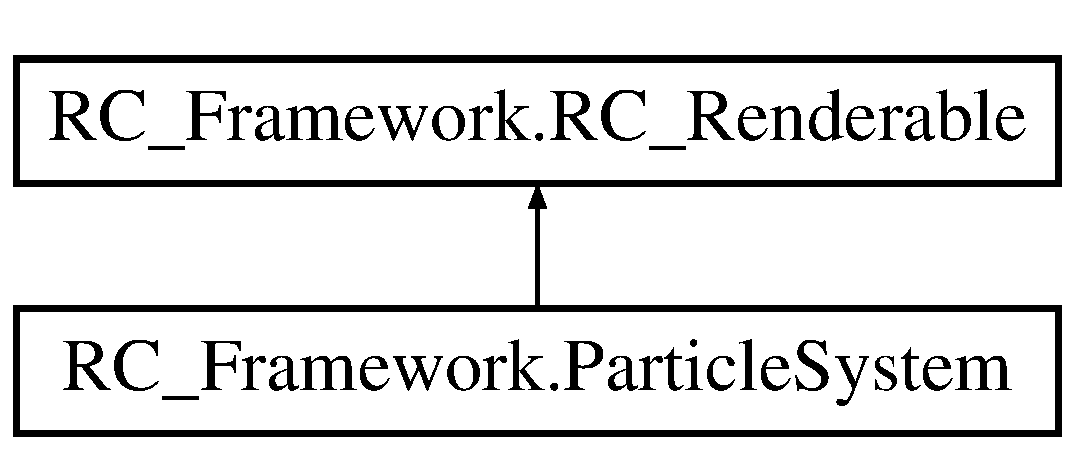
\includegraphics[height=2.000000cm]{class_r_c___framework_1_1_particle_system}
\end{center}
\end{figure}
\subsection*{Public Member Functions}
\begin{DoxyCompactItemize}
\item 
\mbox{\hyperlink{class_r_c___framework_1_1_particle_system_a9baad9b596967f62ce758557a4baecdc}{Particle\+System}} (Vector2 posZ, int MaxnumZ, int ticks\+System\+DurationZ, int random\+Seed)
\item 
override void \mbox{\hyperlink{class_r_c___framework_1_1_particle_system_ac96aa1743b45944d102ddf01d67452c1}{reset}} ()
\item 
void \mbox{\hyperlink{class_r_c___framework_1_1_particle_system_a145da945b2d05fe75735e007796fc158}{set\+Mandatory1}} (Texture2D texZ, Vector2 start\+SizeZ, Vector2 end\+SizeZ, Color start\+ColorZ, Color end\+ColorZ)
\item 
void \mbox{\hyperlink{class_r_c___framework_1_1_particle_system_af7698934f85ed2081ba236db023fa004}{set\+Mandatory2}} (int total\+Number\+To\+MakeZ, int initial\+Number\+To\+MakeZ, int subsequent\+Number\+To\+MakeZ, int ticks\+Between\+Make\+EventsZ, int random10000\+TomakeZ)
\item 
void \mbox{\hyperlink{class_r_c___framework_1_1_particle_system_a4a7d1047a8f891f66c5cc2f290520107}{set\+Mandatory3}} (int ticks\+Particle\+DurationZ, Rectangle boundsZ)
\item 
void \mbox{\hyperlink{class_r_c___framework_1_1_particle_system_a7b3f6b8c93d32699592cb3737f449fa9}{set\+Mandatory4}} (Vector2 deltaZ, Vector2 initial\+VelosityZ, Vector2 initial\+Velosity\+RandomZ)
\item 
void \mbox{\hyperlink{class_r_c___framework_1_1_particle_system_a7757ad5d623f0f275e07dff00d37efd5}{activate}} ()
\item 
void \mbox{\hyperlink{class_r_c___framework_1_1_particle_system_a5203abf6d889ed63facf7c5262a48733}{de\+Activate}} ()
\item 
void \mbox{\hyperlink{class_r_c___framework_1_1_particle_system_a229864cc0b24df0bab9e43b07fdd4b8d}{if\+Safe\+To\+Remove\+De\+Activate}} ()
\item 
void \mbox{\hyperlink{class_r_c___framework_1_1_particle_system_a80b4943e107e2ee29218ebb358e5e0bf}{make\+Particles}} (int num)
\item 
int \mbox{\hyperlink{class_r_c___framework_1_1_particle_system_ad97ae58b6cb5679a4f9ce02cb4d714ea}{Contains}} (Vector2 point)
\begin{DoxyCompactList}\small\item\em tests if any active particle contains the point Returns -\/1 if it misses all particles otherwise it returns the particle number \end{DoxyCompactList}\item 
void \mbox{\hyperlink{class_r_c___framework_1_1_particle_system_af6c1685abb024ef387dc160fb1db4bad}{set\+Way\+List\+Count}} (int wlc)
\item 
override void \mbox{\hyperlink{class_r_c___framework_1_1_particle_system_a658681cf664bb153b4defb6a861bc721}{Update}} (Game\+Time game\+Time)
\item 
void \mbox{\hyperlink{class_r_c___framework_1_1_particle_system_a8097f166bded1c9a4e511e4d22e09541}{update\+Particles}} ()
\item 
override void \mbox{\hyperlink{class_r_c___framework_1_1_particle_system_a2cb9a22f944e93697fff3128a1d3ddb6}{Draw}} (Sprite\+Batch sp)
\begin{DoxyCompactList}\small\item\em Standard draw routine which assumes the renderable knows where it is \end{DoxyCompactList}\end{DoxyCompactItemize}
\subsection*{Public Attributes}
\begin{DoxyCompactItemize}
\item 
float \mbox{\hyperlink{class_r_c___framework_1_1_particle_system_a6f21e255387e86b9352f7ba362f4737c}{inital\+Angle\+Low}} = 0
\item 
float \mbox{\hyperlink{class_r_c___framework_1_1_particle_system_a5b6110ac4cdeffb18a96fdc5a3782956}{inital\+Angle\+High}} = 0
\item 
float \mbox{\hyperlink{class_r_c___framework_1_1_particle_system_a5703bd6030e08d2047d574d269f936e0}{inital\+Velocity\+Low}} = 0
\item 
float \mbox{\hyperlink{class_r_c___framework_1_1_particle_system_acf82c04377b18711b36f2d31ae460ad9}{inital\+Velocity\+High}} = 0
\end{DoxyCompactItemize}
\subsection*{Properties}
\begin{DoxyCompactItemize}
\item 
Texture2D \mbox{\hyperlink{class_r_c___framework_1_1_particle_system_a742f2d81c88deed1f55ec5bbf70f4ab9}{tex}}\hspace{0.3cm}{\ttfamily  \mbox{[}get, set\mbox{]}}
\item 
bool \mbox{\hyperlink{class_r_c___framework_1_1_particle_system_aa8cf7d8f7c1a323cde4dd0016aa4bd9d}{generation}}\hspace{0.3cm}{\ttfamily  \mbox{[}get, set\mbox{]}}
\item 
Vector2 \mbox{\hyperlink{class_r_c___framework_1_1_particle_system_ac4f852ac1384ce4392696641a4a4be25}{start\+Size}}\hspace{0.3cm}{\ttfamily  \mbox{[}get, set\mbox{]}}
\item 
Vector2 \mbox{\hyperlink{class_r_c___framework_1_1_particle_system_a17842ac5d898f4778ca7e4252cab591f}{end\+Size}}\hspace{0.3cm}{\ttfamily  \mbox{[}get, set\mbox{]}}
\item 
Vector2 \mbox{\hyperlink{class_r_c___framework_1_1_particle_system_a47f4e639b5021d6088461bb8034853d0}{sys\+Pos}}\hspace{0.3cm}{\ttfamily  \mbox{[}get, set\mbox{]}}
\item 
Color \mbox{\hyperlink{class_r_c___framework_1_1_particle_system_ae2d934fe4a2fe39abb50434f3f205206}{start\+Color}}\hspace{0.3cm}{\ttfamily  \mbox{[}get, set\mbox{]}}
\item 
Color \mbox{\hyperlink{class_r_c___framework_1_1_particle_system_a5c7fb74e67dcfd8af485fd0ad0aefe94}{end\+Color}}\hspace{0.3cm}{\ttfamily  \mbox{[}get, set\mbox{]}}
\item 
int \mbox{\hyperlink{class_r_c___framework_1_1_particle_system_a618679965392a7e57dd71e7ea64a350d}{ticks\+System\+Duration}}\hspace{0.3cm}{\ttfamily  \mbox{[}get, set\mbox{]}}
\item 
Rectangle \mbox{\hyperlink{class_r_c___framework_1_1_particle_system_a3f28ceb4c26eec9d8ddd5b957f4a5c7c}{bounds}}\hspace{0.3cm}{\ttfamily  \mbox{[}get, set\mbox{]}}
\item 
Vector2 \mbox{\hyperlink{class_r_c___framework_1_1_particle_system_afeebe9c2046c500af1da292b48041054}{delta}}\hspace{0.3cm}{\ttfamily  \mbox{[}get, set\mbox{]}}
\item 
Vector2 \mbox{\hyperlink{class_r_c___framework_1_1_particle_system_a822fa383fdd59536a220d8c6389159d8}{random\+Delta}}\hspace{0.3cm}{\ttfamily  \mbox{[}get, set\mbox{]}}
\item 
Vector2 \mbox{\hyperlink{class_r_c___framework_1_1_particle_system_ad9da77ebbe3e8f1425ef176fef680907}{wind\+Delta}}\hspace{0.3cm}{\ttfamily  \mbox{[}get, set\mbox{]}}
\item 
Vector2 \mbox{\hyperlink{class_r_c___framework_1_1_particle_system_a1ba7b70a31e8c6cc10cc3f59f5250db1}{resistance}}\hspace{0.3cm}{\ttfamily  \mbox{[}get, set\mbox{]}}
\item 
Vector2 \mbox{\hyperlink{class_r_c___framework_1_1_particle_system_ae40ff073fcaf19f02f4a44904441ccca}{initial\+Velosity}}\hspace{0.3cm}{\ttfamily  \mbox{[}get, set\mbox{]}}
\item 
Vector2 \mbox{\hyperlink{class_r_c___framework_1_1_particle_system_a52c86010adb7aacffff157a77786daf0}{initial\+Velosity\+Random}}\hspace{0.3cm}{\ttfamily  \mbox{[}get, set\mbox{]}}
\item 
int \mbox{\hyperlink{class_r_c___framework_1_1_particle_system_a1a04c770e267f6c595cef5644a0deae7}{Origin}}\hspace{0.3cm}{\ttfamily  \mbox{[}get, set\mbox{]}}
\item 
Rectangle \mbox{\hyperlink{class_r_c___framework_1_1_particle_system_a3f614b6db7f50a6367d7732160b6cef1}{origin\+Rectangle}}\hspace{0.3cm}{\ttfamily  \mbox{[}get, set\mbox{]}}
\item 
\mbox{\hyperlink{class_r_c___framework_1_1_way_point_list}{Way\+Point\+List}} \mbox{\hyperlink{class_r_c___framework_1_1_particle_system_aa8187c210d815f3e727c3666542513ca}{origin\+Way\+List}}\hspace{0.3cm}{\ttfamily  \mbox{[}get, set\mbox{]}}
\item 
int \mbox{\hyperlink{class_r_c___framework_1_1_particle_system_ae799d7d003858a97b66e94210fc95453}{total\+Number\+To\+Make}}\hspace{0.3cm}{\ttfamily  \mbox{[}get, set\mbox{]}}
\item 
int \mbox{\hyperlink{class_r_c___framework_1_1_particle_system_a62c4c1f5a709872b3711ed50404fe673}{initial\+Number\+To\+Make}}\hspace{0.3cm}{\ttfamily  \mbox{[}get, set\mbox{]}}
\item 
int \mbox{\hyperlink{class_r_c___framework_1_1_particle_system_a1f5308e212ae17bcdd21cc7ac1516f23}{subsequent\+Number\+To\+Make}}\hspace{0.3cm}{\ttfamily  \mbox{[}get, set\mbox{]}}
\item 
int \mbox{\hyperlink{class_r_c___framework_1_1_particle_system_a7f84c6b6e2d4f0314e6ab67e8a835b5a}{ticks\+Between\+Make\+Events}}\hspace{0.3cm}{\ttfamily  \mbox{[}get, set\mbox{]}}
\item 
int \mbox{\hyperlink{class_r_c___framework_1_1_particle_system_ae1051896325086ff0081894a391735a8}{random10000\+Tomake}}\hspace{0.3cm}{\ttfamily  \mbox{[}get, set\mbox{]}}
\item 
int \mbox{\hyperlink{class_r_c___framework_1_1_particle_system_ab467807a417cc9f022d4ef7bb4561035}{ticks\+Particle\+Duration}}\hspace{0.3cm}{\ttfamily  \mbox{[}get, set\mbox{]}}
\item 
bool \mbox{\hyperlink{class_r_c___framework_1_1_particle_system_af2fb2ff9ebf53545b72d20c0e52db834}{set\+Display\+Angle}}\hspace{0.3cm}{\ttfamily  \mbox{[}get, set\mbox{]}}
\item 
float \mbox{\hyperlink{class_r_c___framework_1_1_particle_system_a9e0e6de2a6683d3a9deb7a762222ab2d}{display\+Angle\+Offset}}\hspace{0.3cm}{\ttfamily  \mbox{[}get, set\mbox{]}}
\item 
int \mbox{\hyperlink{class_r_c___framework_1_1_particle_system_a0b390b18ea379c0a285cad7f02d1cafe}{move\+Towards}}\hspace{0.3cm}{\ttfamily  \mbox{[}get, set\mbox{]}}
\begin{DoxyCompactList}\small\item\em defines override particle movement 0 = nix -\/ just use other movement params ~\newline
1 = towards move\+Towards\+Pos 2 = away from move\+Towards\+Pos 3 = drift towards move\+Towards\+Pos 4 = drift away from move\+Towards\+Pos \end{DoxyCompactList}\item 
Vector2 \mbox{\hyperlink{class_r_c___framework_1_1_particle_system_a863bb790d4e1c5ed363ece08509b96b6}{move\+Towards\+Pos}}\hspace{0.3cm}{\ttfamily  \mbox{[}get, set\mbox{]}}
\item 
float \mbox{\hyperlink{class_r_c___framework_1_1_particle_system_a7d438b6f40ce329bd24ada1fafdfa020}{move\+To\+Drift}}\hspace{0.3cm}{\ttfamily  \mbox{[}get, set\mbox{]}}
\end{DoxyCompactItemize}


\subsection{Constructor \& Destructor Documentation}
\mbox{\Hypertarget{class_r_c___framework_1_1_particle_system_a9baad9b596967f62ce758557a4baecdc}\label{class_r_c___framework_1_1_particle_system_a9baad9b596967f62ce758557a4baecdc}} 
\index{R\+C\+\_\+\+Framework\+::\+Particle\+System@{R\+C\+\_\+\+Framework\+::\+Particle\+System}!Particle\+System@{Particle\+System}}
\index{Particle\+System@{Particle\+System}!R\+C\+\_\+\+Framework\+::\+Particle\+System@{R\+C\+\_\+\+Framework\+::\+Particle\+System}}
\subsubsection{\texorpdfstring{Particle\+System()}{ParticleSystem()}}
{\footnotesize\ttfamily R\+C\+\_\+\+Framework.\+Particle\+System.\+Particle\+System (\begin{DoxyParamCaption}\item[{Vector2}]{posZ,  }\item[{int}]{MaxnumZ,  }\item[{int}]{ticks\+System\+DurationZ,  }\item[{int}]{random\+Seed }\end{DoxyParamCaption})}



\subsection{Member Function Documentation}
\mbox{\Hypertarget{class_r_c___framework_1_1_particle_system_a7757ad5d623f0f275e07dff00d37efd5}\label{class_r_c___framework_1_1_particle_system_a7757ad5d623f0f275e07dff00d37efd5}} 
\index{R\+C\+\_\+\+Framework\+::\+Particle\+System@{R\+C\+\_\+\+Framework\+::\+Particle\+System}!activate@{activate}}
\index{activate@{activate}!R\+C\+\_\+\+Framework\+::\+Particle\+System@{R\+C\+\_\+\+Framework\+::\+Particle\+System}}
\subsubsection{\texorpdfstring{activate()}{activate()}}
{\footnotesize\ttfamily void R\+C\+\_\+\+Framework.\+Particle\+System.\+activate (\begin{DoxyParamCaption}{ }\end{DoxyParamCaption})}

\mbox{\Hypertarget{class_r_c___framework_1_1_particle_system_ad97ae58b6cb5679a4f9ce02cb4d714ea}\label{class_r_c___framework_1_1_particle_system_ad97ae58b6cb5679a4f9ce02cb4d714ea}} 
\index{R\+C\+\_\+\+Framework\+::\+Particle\+System@{R\+C\+\_\+\+Framework\+::\+Particle\+System}!Contains@{Contains}}
\index{Contains@{Contains}!R\+C\+\_\+\+Framework\+::\+Particle\+System@{R\+C\+\_\+\+Framework\+::\+Particle\+System}}
\subsubsection{\texorpdfstring{Contains()}{Contains()}}
{\footnotesize\ttfamily int R\+C\+\_\+\+Framework.\+Particle\+System.\+Contains (\begin{DoxyParamCaption}\item[{Vector2}]{point }\end{DoxyParamCaption})}



tests if any active particle contains the point Returns -\/1 if it misses all particles otherwise it returns the particle number 


\begin{DoxyParams}{Parameters}
{\em point} & \\
\hline
\end{DoxyParams}
\begin{DoxyReturn}{Returns}

\end{DoxyReturn}
\mbox{\Hypertarget{class_r_c___framework_1_1_particle_system_a5203abf6d889ed63facf7c5262a48733}\label{class_r_c___framework_1_1_particle_system_a5203abf6d889ed63facf7c5262a48733}} 
\index{R\+C\+\_\+\+Framework\+::\+Particle\+System@{R\+C\+\_\+\+Framework\+::\+Particle\+System}!de\+Activate@{de\+Activate}}
\index{de\+Activate@{de\+Activate}!R\+C\+\_\+\+Framework\+::\+Particle\+System@{R\+C\+\_\+\+Framework\+::\+Particle\+System}}
\subsubsection{\texorpdfstring{de\+Activate()}{deActivate()}}
{\footnotesize\ttfamily void R\+C\+\_\+\+Framework.\+Particle\+System.\+de\+Activate (\begin{DoxyParamCaption}{ }\end{DoxyParamCaption})}

\mbox{\Hypertarget{class_r_c___framework_1_1_particle_system_a2cb9a22f944e93697fff3128a1d3ddb6}\label{class_r_c___framework_1_1_particle_system_a2cb9a22f944e93697fff3128a1d3ddb6}} 
\index{R\+C\+\_\+\+Framework\+::\+Particle\+System@{R\+C\+\_\+\+Framework\+::\+Particle\+System}!Draw@{Draw}}
\index{Draw@{Draw}!R\+C\+\_\+\+Framework\+::\+Particle\+System@{R\+C\+\_\+\+Framework\+::\+Particle\+System}}
\subsubsection{\texorpdfstring{Draw()}{Draw()}}
{\footnotesize\ttfamily override void R\+C\+\_\+\+Framework.\+Particle\+System.\+Draw (\begin{DoxyParamCaption}\item[{Sprite\+Batch}]{sb }\end{DoxyParamCaption})\hspace{0.3cm}{\ttfamily [virtual]}}



Standard draw routine which assumes the renderable knows where it is 


\begin{DoxyParams}{Parameters}
{\em sb} & \\
\hline
\end{DoxyParams}


Reimplemented from \mbox{\hyperlink{class_r_c___framework_1_1_r_c___renderable_acc26db34e382a25a989c4c0dd0354b23}{R\+C\+\_\+\+Framework.\+R\+C\+\_\+\+Renderable}}.

\mbox{\Hypertarget{class_r_c___framework_1_1_particle_system_a229864cc0b24df0bab9e43b07fdd4b8d}\label{class_r_c___framework_1_1_particle_system_a229864cc0b24df0bab9e43b07fdd4b8d}} 
\index{R\+C\+\_\+\+Framework\+::\+Particle\+System@{R\+C\+\_\+\+Framework\+::\+Particle\+System}!if\+Safe\+To\+Remove\+De\+Activate@{if\+Safe\+To\+Remove\+De\+Activate}}
\index{if\+Safe\+To\+Remove\+De\+Activate@{if\+Safe\+To\+Remove\+De\+Activate}!R\+C\+\_\+\+Framework\+::\+Particle\+System@{R\+C\+\_\+\+Framework\+::\+Particle\+System}}
\subsubsection{\texorpdfstring{if\+Safe\+To\+Remove\+De\+Activate()}{ifSafeToRemoveDeActivate()}}
{\footnotesize\ttfamily void R\+C\+\_\+\+Framework.\+Particle\+System.\+if\+Safe\+To\+Remove\+De\+Activate (\begin{DoxyParamCaption}{ }\end{DoxyParamCaption})}

\mbox{\Hypertarget{class_r_c___framework_1_1_particle_system_a80b4943e107e2ee29218ebb358e5e0bf}\label{class_r_c___framework_1_1_particle_system_a80b4943e107e2ee29218ebb358e5e0bf}} 
\index{R\+C\+\_\+\+Framework\+::\+Particle\+System@{R\+C\+\_\+\+Framework\+::\+Particle\+System}!make\+Particles@{make\+Particles}}
\index{make\+Particles@{make\+Particles}!R\+C\+\_\+\+Framework\+::\+Particle\+System@{R\+C\+\_\+\+Framework\+::\+Particle\+System}}
\subsubsection{\texorpdfstring{make\+Particles()}{makeParticles()}}
{\footnotesize\ttfamily void R\+C\+\_\+\+Framework.\+Particle\+System.\+make\+Particles (\begin{DoxyParamCaption}\item[{int}]{num }\end{DoxyParamCaption})}

\mbox{\Hypertarget{class_r_c___framework_1_1_particle_system_ac96aa1743b45944d102ddf01d67452c1}\label{class_r_c___framework_1_1_particle_system_ac96aa1743b45944d102ddf01d67452c1}} 
\index{R\+C\+\_\+\+Framework\+::\+Particle\+System@{R\+C\+\_\+\+Framework\+::\+Particle\+System}!reset@{reset}}
\index{reset@{reset}!R\+C\+\_\+\+Framework\+::\+Particle\+System@{R\+C\+\_\+\+Framework\+::\+Particle\+System}}
\subsubsection{\texorpdfstring{reset()}{reset()}}
{\footnotesize\ttfamily override void R\+C\+\_\+\+Framework.\+Particle\+System.\+reset (\begin{DoxyParamCaption}{ }\end{DoxyParamCaption})\hspace{0.3cm}{\ttfamily [virtual]}}



Reimplemented from \mbox{\hyperlink{class_r_c___framework_1_1_r_c___renderable_ae65ce69704d15963789f421b58618b1f}{R\+C\+\_\+\+Framework.\+R\+C\+\_\+\+Renderable}}.

\mbox{\Hypertarget{class_r_c___framework_1_1_particle_system_a145da945b2d05fe75735e007796fc158}\label{class_r_c___framework_1_1_particle_system_a145da945b2d05fe75735e007796fc158}} 
\index{R\+C\+\_\+\+Framework\+::\+Particle\+System@{R\+C\+\_\+\+Framework\+::\+Particle\+System}!set\+Mandatory1@{set\+Mandatory1}}
\index{set\+Mandatory1@{set\+Mandatory1}!R\+C\+\_\+\+Framework\+::\+Particle\+System@{R\+C\+\_\+\+Framework\+::\+Particle\+System}}
\subsubsection{\texorpdfstring{set\+Mandatory1()}{setMandatory1()}}
{\footnotesize\ttfamily void R\+C\+\_\+\+Framework.\+Particle\+System.\+set\+Mandatory1 (\begin{DoxyParamCaption}\item[{Texture2D}]{texZ,  }\item[{Vector2}]{start\+SizeZ,  }\item[{Vector2}]{end\+SizeZ,  }\item[{Color}]{start\+ColorZ,  }\item[{Color}]{end\+ColorZ }\end{DoxyParamCaption})}

\mbox{\Hypertarget{class_r_c___framework_1_1_particle_system_af7698934f85ed2081ba236db023fa004}\label{class_r_c___framework_1_1_particle_system_af7698934f85ed2081ba236db023fa004}} 
\index{R\+C\+\_\+\+Framework\+::\+Particle\+System@{R\+C\+\_\+\+Framework\+::\+Particle\+System}!set\+Mandatory2@{set\+Mandatory2}}
\index{set\+Mandatory2@{set\+Mandatory2}!R\+C\+\_\+\+Framework\+::\+Particle\+System@{R\+C\+\_\+\+Framework\+::\+Particle\+System}}
\subsubsection{\texorpdfstring{set\+Mandatory2()}{setMandatory2()}}
{\footnotesize\ttfamily void R\+C\+\_\+\+Framework.\+Particle\+System.\+set\+Mandatory2 (\begin{DoxyParamCaption}\item[{int}]{total\+Number\+To\+MakeZ,  }\item[{int}]{initial\+Number\+To\+MakeZ,  }\item[{int}]{subsequent\+Number\+To\+MakeZ,  }\item[{int}]{ticks\+Between\+Make\+EventsZ,  }\item[{int}]{random10000\+TomakeZ }\end{DoxyParamCaption})}

\mbox{\Hypertarget{class_r_c___framework_1_1_particle_system_a4a7d1047a8f891f66c5cc2f290520107}\label{class_r_c___framework_1_1_particle_system_a4a7d1047a8f891f66c5cc2f290520107}} 
\index{R\+C\+\_\+\+Framework\+::\+Particle\+System@{R\+C\+\_\+\+Framework\+::\+Particle\+System}!set\+Mandatory3@{set\+Mandatory3}}
\index{set\+Mandatory3@{set\+Mandatory3}!R\+C\+\_\+\+Framework\+::\+Particle\+System@{R\+C\+\_\+\+Framework\+::\+Particle\+System}}
\subsubsection{\texorpdfstring{set\+Mandatory3()}{setMandatory3()}}
{\footnotesize\ttfamily void R\+C\+\_\+\+Framework.\+Particle\+System.\+set\+Mandatory3 (\begin{DoxyParamCaption}\item[{int}]{ticks\+Particle\+DurationZ,  }\item[{Rectangle}]{boundsZ }\end{DoxyParamCaption})}

\mbox{\Hypertarget{class_r_c___framework_1_1_particle_system_a7b3f6b8c93d32699592cb3737f449fa9}\label{class_r_c___framework_1_1_particle_system_a7b3f6b8c93d32699592cb3737f449fa9}} 
\index{R\+C\+\_\+\+Framework\+::\+Particle\+System@{R\+C\+\_\+\+Framework\+::\+Particle\+System}!set\+Mandatory4@{set\+Mandatory4}}
\index{set\+Mandatory4@{set\+Mandatory4}!R\+C\+\_\+\+Framework\+::\+Particle\+System@{R\+C\+\_\+\+Framework\+::\+Particle\+System}}
\subsubsection{\texorpdfstring{set\+Mandatory4()}{setMandatory4()}}
{\footnotesize\ttfamily void R\+C\+\_\+\+Framework.\+Particle\+System.\+set\+Mandatory4 (\begin{DoxyParamCaption}\item[{Vector2}]{deltaZ,  }\item[{Vector2}]{initial\+VelosityZ,  }\item[{Vector2}]{initial\+Velosity\+RandomZ }\end{DoxyParamCaption})}

\mbox{\Hypertarget{class_r_c___framework_1_1_particle_system_af6c1685abb024ef387dc160fb1db4bad}\label{class_r_c___framework_1_1_particle_system_af6c1685abb024ef387dc160fb1db4bad}} 
\index{R\+C\+\_\+\+Framework\+::\+Particle\+System@{R\+C\+\_\+\+Framework\+::\+Particle\+System}!set\+Way\+List\+Count@{set\+Way\+List\+Count}}
\index{set\+Way\+List\+Count@{set\+Way\+List\+Count}!R\+C\+\_\+\+Framework\+::\+Particle\+System@{R\+C\+\_\+\+Framework\+::\+Particle\+System}}
\subsubsection{\texorpdfstring{set\+Way\+List\+Count()}{setWayListCount()}}
{\footnotesize\ttfamily void R\+C\+\_\+\+Framework.\+Particle\+System.\+set\+Way\+List\+Count (\begin{DoxyParamCaption}\item[{int}]{wlc }\end{DoxyParamCaption})}

\mbox{\Hypertarget{class_r_c___framework_1_1_particle_system_a658681cf664bb153b4defb6a861bc721}\label{class_r_c___framework_1_1_particle_system_a658681cf664bb153b4defb6a861bc721}} 
\index{R\+C\+\_\+\+Framework\+::\+Particle\+System@{R\+C\+\_\+\+Framework\+::\+Particle\+System}!Update@{Update}}
\index{Update@{Update}!R\+C\+\_\+\+Framework\+::\+Particle\+System@{R\+C\+\_\+\+Framework\+::\+Particle\+System}}
\subsubsection{\texorpdfstring{Update()}{Update()}}
{\footnotesize\ttfamily override void R\+C\+\_\+\+Framework.\+Particle\+System.\+Update (\begin{DoxyParamCaption}\item[{Game\+Time}]{game\+Time }\end{DoxyParamCaption})\hspace{0.3cm}{\ttfamily [virtual]}}



Reimplemented from \mbox{\hyperlink{class_r_c___framework_1_1_r_c___renderable_a5745bedc7ba0587aa1e1d8563c357228}{R\+C\+\_\+\+Framework.\+R\+C\+\_\+\+Renderable}}.

\mbox{\Hypertarget{class_r_c___framework_1_1_particle_system_a8097f166bded1c9a4e511e4d22e09541}\label{class_r_c___framework_1_1_particle_system_a8097f166bded1c9a4e511e4d22e09541}} 
\index{R\+C\+\_\+\+Framework\+::\+Particle\+System@{R\+C\+\_\+\+Framework\+::\+Particle\+System}!update\+Particles@{update\+Particles}}
\index{update\+Particles@{update\+Particles}!R\+C\+\_\+\+Framework\+::\+Particle\+System@{R\+C\+\_\+\+Framework\+::\+Particle\+System}}
\subsubsection{\texorpdfstring{update\+Particles()}{updateParticles()}}
{\footnotesize\ttfamily void R\+C\+\_\+\+Framework.\+Particle\+System.\+update\+Particles (\begin{DoxyParamCaption}{ }\end{DoxyParamCaption})}



\subsection{Member Data Documentation}
\mbox{\Hypertarget{class_r_c___framework_1_1_particle_system_a5b6110ac4cdeffb18a96fdc5a3782956}\label{class_r_c___framework_1_1_particle_system_a5b6110ac4cdeffb18a96fdc5a3782956}} 
\index{R\+C\+\_\+\+Framework\+::\+Particle\+System@{R\+C\+\_\+\+Framework\+::\+Particle\+System}!inital\+Angle\+High@{inital\+Angle\+High}}
\index{inital\+Angle\+High@{inital\+Angle\+High}!R\+C\+\_\+\+Framework\+::\+Particle\+System@{R\+C\+\_\+\+Framework\+::\+Particle\+System}}
\subsubsection{\texorpdfstring{inital\+Angle\+High}{initalAngleHigh}}
{\footnotesize\ttfamily float R\+C\+\_\+\+Framework.\+Particle\+System.\+inital\+Angle\+High = 0}

\mbox{\Hypertarget{class_r_c___framework_1_1_particle_system_a6f21e255387e86b9352f7ba362f4737c}\label{class_r_c___framework_1_1_particle_system_a6f21e255387e86b9352f7ba362f4737c}} 
\index{R\+C\+\_\+\+Framework\+::\+Particle\+System@{R\+C\+\_\+\+Framework\+::\+Particle\+System}!inital\+Angle\+Low@{inital\+Angle\+Low}}
\index{inital\+Angle\+Low@{inital\+Angle\+Low}!R\+C\+\_\+\+Framework\+::\+Particle\+System@{R\+C\+\_\+\+Framework\+::\+Particle\+System}}
\subsubsection{\texorpdfstring{inital\+Angle\+Low}{initalAngleLow}}
{\footnotesize\ttfamily float R\+C\+\_\+\+Framework.\+Particle\+System.\+inital\+Angle\+Low = 0}

\mbox{\Hypertarget{class_r_c___framework_1_1_particle_system_acf82c04377b18711b36f2d31ae460ad9}\label{class_r_c___framework_1_1_particle_system_acf82c04377b18711b36f2d31ae460ad9}} 
\index{R\+C\+\_\+\+Framework\+::\+Particle\+System@{R\+C\+\_\+\+Framework\+::\+Particle\+System}!inital\+Velocity\+High@{inital\+Velocity\+High}}
\index{inital\+Velocity\+High@{inital\+Velocity\+High}!R\+C\+\_\+\+Framework\+::\+Particle\+System@{R\+C\+\_\+\+Framework\+::\+Particle\+System}}
\subsubsection{\texorpdfstring{inital\+Velocity\+High}{initalVelocityHigh}}
{\footnotesize\ttfamily float R\+C\+\_\+\+Framework.\+Particle\+System.\+inital\+Velocity\+High = 0}

\mbox{\Hypertarget{class_r_c___framework_1_1_particle_system_a5703bd6030e08d2047d574d269f936e0}\label{class_r_c___framework_1_1_particle_system_a5703bd6030e08d2047d574d269f936e0}} 
\index{R\+C\+\_\+\+Framework\+::\+Particle\+System@{R\+C\+\_\+\+Framework\+::\+Particle\+System}!inital\+Velocity\+Low@{inital\+Velocity\+Low}}
\index{inital\+Velocity\+Low@{inital\+Velocity\+Low}!R\+C\+\_\+\+Framework\+::\+Particle\+System@{R\+C\+\_\+\+Framework\+::\+Particle\+System}}
\subsubsection{\texorpdfstring{inital\+Velocity\+Low}{initalVelocityLow}}
{\footnotesize\ttfamily float R\+C\+\_\+\+Framework.\+Particle\+System.\+inital\+Velocity\+Low = 0}



\subsection{Property Documentation}
\mbox{\Hypertarget{class_r_c___framework_1_1_particle_system_a3f28ceb4c26eec9d8ddd5b957f4a5c7c}\label{class_r_c___framework_1_1_particle_system_a3f28ceb4c26eec9d8ddd5b957f4a5c7c}} 
\index{R\+C\+\_\+\+Framework\+::\+Particle\+System@{R\+C\+\_\+\+Framework\+::\+Particle\+System}!bounds@{bounds}}
\index{bounds@{bounds}!R\+C\+\_\+\+Framework\+::\+Particle\+System@{R\+C\+\_\+\+Framework\+::\+Particle\+System}}
\subsubsection{\texorpdfstring{bounds}{bounds}}
{\footnotesize\ttfamily Rectangle R\+C\+\_\+\+Framework.\+Particle\+System.\+bounds\hspace{0.3cm}{\ttfamily [get]}, {\ttfamily [set]}}

\mbox{\Hypertarget{class_r_c___framework_1_1_particle_system_afeebe9c2046c500af1da292b48041054}\label{class_r_c___framework_1_1_particle_system_afeebe9c2046c500af1da292b48041054}} 
\index{R\+C\+\_\+\+Framework\+::\+Particle\+System@{R\+C\+\_\+\+Framework\+::\+Particle\+System}!delta@{delta}}
\index{delta@{delta}!R\+C\+\_\+\+Framework\+::\+Particle\+System@{R\+C\+\_\+\+Framework\+::\+Particle\+System}}
\subsubsection{\texorpdfstring{delta}{delta}}
{\footnotesize\ttfamily Vector2 R\+C\+\_\+\+Framework.\+Particle\+System.\+delta\hspace{0.3cm}{\ttfamily [get]}, {\ttfamily [set]}}

\mbox{\Hypertarget{class_r_c___framework_1_1_particle_system_a9e0e6de2a6683d3a9deb7a762222ab2d}\label{class_r_c___framework_1_1_particle_system_a9e0e6de2a6683d3a9deb7a762222ab2d}} 
\index{R\+C\+\_\+\+Framework\+::\+Particle\+System@{R\+C\+\_\+\+Framework\+::\+Particle\+System}!display\+Angle\+Offset@{display\+Angle\+Offset}}
\index{display\+Angle\+Offset@{display\+Angle\+Offset}!R\+C\+\_\+\+Framework\+::\+Particle\+System@{R\+C\+\_\+\+Framework\+::\+Particle\+System}}
\subsubsection{\texorpdfstring{display\+Angle\+Offset}{displayAngleOffset}}
{\footnotesize\ttfamily float R\+C\+\_\+\+Framework.\+Particle\+System.\+display\+Angle\+Offset\hspace{0.3cm}{\ttfamily [get]}, {\ttfamily [set]}}

\mbox{\Hypertarget{class_r_c___framework_1_1_particle_system_a5c7fb74e67dcfd8af485fd0ad0aefe94}\label{class_r_c___framework_1_1_particle_system_a5c7fb74e67dcfd8af485fd0ad0aefe94}} 
\index{R\+C\+\_\+\+Framework\+::\+Particle\+System@{R\+C\+\_\+\+Framework\+::\+Particle\+System}!end\+Color@{end\+Color}}
\index{end\+Color@{end\+Color}!R\+C\+\_\+\+Framework\+::\+Particle\+System@{R\+C\+\_\+\+Framework\+::\+Particle\+System}}
\subsubsection{\texorpdfstring{end\+Color}{endColor}}
{\footnotesize\ttfamily Color R\+C\+\_\+\+Framework.\+Particle\+System.\+end\+Color\hspace{0.3cm}{\ttfamily [get]}, {\ttfamily [set]}}

\mbox{\Hypertarget{class_r_c___framework_1_1_particle_system_a17842ac5d898f4778ca7e4252cab591f}\label{class_r_c___framework_1_1_particle_system_a17842ac5d898f4778ca7e4252cab591f}} 
\index{R\+C\+\_\+\+Framework\+::\+Particle\+System@{R\+C\+\_\+\+Framework\+::\+Particle\+System}!end\+Size@{end\+Size}}
\index{end\+Size@{end\+Size}!R\+C\+\_\+\+Framework\+::\+Particle\+System@{R\+C\+\_\+\+Framework\+::\+Particle\+System}}
\subsubsection{\texorpdfstring{end\+Size}{endSize}}
{\footnotesize\ttfamily Vector2 R\+C\+\_\+\+Framework.\+Particle\+System.\+end\+Size\hspace{0.3cm}{\ttfamily [get]}, {\ttfamily [set]}}

\mbox{\Hypertarget{class_r_c___framework_1_1_particle_system_aa8cf7d8f7c1a323cde4dd0016aa4bd9d}\label{class_r_c___framework_1_1_particle_system_aa8cf7d8f7c1a323cde4dd0016aa4bd9d}} 
\index{R\+C\+\_\+\+Framework\+::\+Particle\+System@{R\+C\+\_\+\+Framework\+::\+Particle\+System}!generation@{generation}}
\index{generation@{generation}!R\+C\+\_\+\+Framework\+::\+Particle\+System@{R\+C\+\_\+\+Framework\+::\+Particle\+System}}
\subsubsection{\texorpdfstring{generation}{generation}}
{\footnotesize\ttfamily bool R\+C\+\_\+\+Framework.\+Particle\+System.\+generation\hspace{0.3cm}{\ttfamily [get]}, {\ttfamily [set]}}

\mbox{\Hypertarget{class_r_c___framework_1_1_particle_system_a62c4c1f5a709872b3711ed50404fe673}\label{class_r_c___framework_1_1_particle_system_a62c4c1f5a709872b3711ed50404fe673}} 
\index{R\+C\+\_\+\+Framework\+::\+Particle\+System@{R\+C\+\_\+\+Framework\+::\+Particle\+System}!initial\+Number\+To\+Make@{initial\+Number\+To\+Make}}
\index{initial\+Number\+To\+Make@{initial\+Number\+To\+Make}!R\+C\+\_\+\+Framework\+::\+Particle\+System@{R\+C\+\_\+\+Framework\+::\+Particle\+System}}
\subsubsection{\texorpdfstring{initial\+Number\+To\+Make}{initialNumberToMake}}
{\footnotesize\ttfamily int R\+C\+\_\+\+Framework.\+Particle\+System.\+initial\+Number\+To\+Make\hspace{0.3cm}{\ttfamily [get]}, {\ttfamily [set]}}

\mbox{\Hypertarget{class_r_c___framework_1_1_particle_system_ae40ff073fcaf19f02f4a44904441ccca}\label{class_r_c___framework_1_1_particle_system_ae40ff073fcaf19f02f4a44904441ccca}} 
\index{R\+C\+\_\+\+Framework\+::\+Particle\+System@{R\+C\+\_\+\+Framework\+::\+Particle\+System}!initial\+Velosity@{initial\+Velosity}}
\index{initial\+Velosity@{initial\+Velosity}!R\+C\+\_\+\+Framework\+::\+Particle\+System@{R\+C\+\_\+\+Framework\+::\+Particle\+System}}
\subsubsection{\texorpdfstring{initial\+Velosity}{initialVelosity}}
{\footnotesize\ttfamily Vector2 R\+C\+\_\+\+Framework.\+Particle\+System.\+initial\+Velosity\hspace{0.3cm}{\ttfamily [get]}, {\ttfamily [set]}}

\mbox{\Hypertarget{class_r_c___framework_1_1_particle_system_a52c86010adb7aacffff157a77786daf0}\label{class_r_c___framework_1_1_particle_system_a52c86010adb7aacffff157a77786daf0}} 
\index{R\+C\+\_\+\+Framework\+::\+Particle\+System@{R\+C\+\_\+\+Framework\+::\+Particle\+System}!initial\+Velosity\+Random@{initial\+Velosity\+Random}}
\index{initial\+Velosity\+Random@{initial\+Velosity\+Random}!R\+C\+\_\+\+Framework\+::\+Particle\+System@{R\+C\+\_\+\+Framework\+::\+Particle\+System}}
\subsubsection{\texorpdfstring{initial\+Velosity\+Random}{initialVelosityRandom}}
{\footnotesize\ttfamily Vector2 R\+C\+\_\+\+Framework.\+Particle\+System.\+initial\+Velosity\+Random\hspace{0.3cm}{\ttfamily [get]}, {\ttfamily [set]}}

\mbox{\Hypertarget{class_r_c___framework_1_1_particle_system_a7d438b6f40ce329bd24ada1fafdfa020}\label{class_r_c___framework_1_1_particle_system_a7d438b6f40ce329bd24ada1fafdfa020}} 
\index{R\+C\+\_\+\+Framework\+::\+Particle\+System@{R\+C\+\_\+\+Framework\+::\+Particle\+System}!move\+To\+Drift@{move\+To\+Drift}}
\index{move\+To\+Drift@{move\+To\+Drift}!R\+C\+\_\+\+Framework\+::\+Particle\+System@{R\+C\+\_\+\+Framework\+::\+Particle\+System}}
\subsubsection{\texorpdfstring{move\+To\+Drift}{moveToDrift}}
{\footnotesize\ttfamily float R\+C\+\_\+\+Framework.\+Particle\+System.\+move\+To\+Drift\hspace{0.3cm}{\ttfamily [get]}, {\ttfamily [set]}}

\mbox{\Hypertarget{class_r_c___framework_1_1_particle_system_a0b390b18ea379c0a285cad7f02d1cafe}\label{class_r_c___framework_1_1_particle_system_a0b390b18ea379c0a285cad7f02d1cafe}} 
\index{R\+C\+\_\+\+Framework\+::\+Particle\+System@{R\+C\+\_\+\+Framework\+::\+Particle\+System}!move\+Towards@{move\+Towards}}
\index{move\+Towards@{move\+Towards}!R\+C\+\_\+\+Framework\+::\+Particle\+System@{R\+C\+\_\+\+Framework\+::\+Particle\+System}}
\subsubsection{\texorpdfstring{move\+Towards}{moveTowards}}
{\footnotesize\ttfamily int R\+C\+\_\+\+Framework.\+Particle\+System.\+move\+Towards\hspace{0.3cm}{\ttfamily [get]}, {\ttfamily [set]}}



defines override particle movement 0 = nix -\/ just use other movement params ~\newline
1 = towards move\+Towards\+Pos 2 = away from move\+Towards\+Pos 3 = drift towards move\+Towards\+Pos 4 = drift away from move\+Towards\+Pos 

\mbox{\Hypertarget{class_r_c___framework_1_1_particle_system_a863bb790d4e1c5ed363ece08509b96b6}\label{class_r_c___framework_1_1_particle_system_a863bb790d4e1c5ed363ece08509b96b6}} 
\index{R\+C\+\_\+\+Framework\+::\+Particle\+System@{R\+C\+\_\+\+Framework\+::\+Particle\+System}!move\+Towards\+Pos@{move\+Towards\+Pos}}
\index{move\+Towards\+Pos@{move\+Towards\+Pos}!R\+C\+\_\+\+Framework\+::\+Particle\+System@{R\+C\+\_\+\+Framework\+::\+Particle\+System}}
\subsubsection{\texorpdfstring{move\+Towards\+Pos}{moveTowardsPos}}
{\footnotesize\ttfamily Vector2 R\+C\+\_\+\+Framework.\+Particle\+System.\+move\+Towards\+Pos\hspace{0.3cm}{\ttfamily [get]}, {\ttfamily [set]}}

\mbox{\Hypertarget{class_r_c___framework_1_1_particle_system_a1a04c770e267f6c595cef5644a0deae7}\label{class_r_c___framework_1_1_particle_system_a1a04c770e267f6c595cef5644a0deae7}} 
\index{R\+C\+\_\+\+Framework\+::\+Particle\+System@{R\+C\+\_\+\+Framework\+::\+Particle\+System}!Origin@{Origin}}
\index{Origin@{Origin}!R\+C\+\_\+\+Framework\+::\+Particle\+System@{R\+C\+\_\+\+Framework\+::\+Particle\+System}}
\subsubsection{\texorpdfstring{Origin}{Origin}}
{\footnotesize\ttfamily int R\+C\+\_\+\+Framework.\+Particle\+System.\+Origin\hspace{0.3cm}{\ttfamily [get]}, {\ttfamily [set]}}

\mbox{\Hypertarget{class_r_c___framework_1_1_particle_system_a3f614b6db7f50a6367d7732160b6cef1}\label{class_r_c___framework_1_1_particle_system_a3f614b6db7f50a6367d7732160b6cef1}} 
\index{R\+C\+\_\+\+Framework\+::\+Particle\+System@{R\+C\+\_\+\+Framework\+::\+Particle\+System}!origin\+Rectangle@{origin\+Rectangle}}
\index{origin\+Rectangle@{origin\+Rectangle}!R\+C\+\_\+\+Framework\+::\+Particle\+System@{R\+C\+\_\+\+Framework\+::\+Particle\+System}}
\subsubsection{\texorpdfstring{origin\+Rectangle}{originRectangle}}
{\footnotesize\ttfamily Rectangle R\+C\+\_\+\+Framework.\+Particle\+System.\+origin\+Rectangle\hspace{0.3cm}{\ttfamily [get]}, {\ttfamily [set]}}

\mbox{\Hypertarget{class_r_c___framework_1_1_particle_system_aa8187c210d815f3e727c3666542513ca}\label{class_r_c___framework_1_1_particle_system_aa8187c210d815f3e727c3666542513ca}} 
\index{R\+C\+\_\+\+Framework\+::\+Particle\+System@{R\+C\+\_\+\+Framework\+::\+Particle\+System}!origin\+Way\+List@{origin\+Way\+List}}
\index{origin\+Way\+List@{origin\+Way\+List}!R\+C\+\_\+\+Framework\+::\+Particle\+System@{R\+C\+\_\+\+Framework\+::\+Particle\+System}}
\subsubsection{\texorpdfstring{origin\+Way\+List}{originWayList}}
{\footnotesize\ttfamily \mbox{\hyperlink{class_r_c___framework_1_1_way_point_list}{Way\+Point\+List}} R\+C\+\_\+\+Framework.\+Particle\+System.\+origin\+Way\+List\hspace{0.3cm}{\ttfamily [get]}, {\ttfamily [set]}}

\mbox{\Hypertarget{class_r_c___framework_1_1_particle_system_ae1051896325086ff0081894a391735a8}\label{class_r_c___framework_1_1_particle_system_ae1051896325086ff0081894a391735a8}} 
\index{R\+C\+\_\+\+Framework\+::\+Particle\+System@{R\+C\+\_\+\+Framework\+::\+Particle\+System}!random10000\+Tomake@{random10000\+Tomake}}
\index{random10000\+Tomake@{random10000\+Tomake}!R\+C\+\_\+\+Framework\+::\+Particle\+System@{R\+C\+\_\+\+Framework\+::\+Particle\+System}}
\subsubsection{\texorpdfstring{random10000\+Tomake}{random10000Tomake}}
{\footnotesize\ttfamily int R\+C\+\_\+\+Framework.\+Particle\+System.\+random10000\+Tomake\hspace{0.3cm}{\ttfamily [get]}, {\ttfamily [set]}}

\mbox{\Hypertarget{class_r_c___framework_1_1_particle_system_a822fa383fdd59536a220d8c6389159d8}\label{class_r_c___framework_1_1_particle_system_a822fa383fdd59536a220d8c6389159d8}} 
\index{R\+C\+\_\+\+Framework\+::\+Particle\+System@{R\+C\+\_\+\+Framework\+::\+Particle\+System}!random\+Delta@{random\+Delta}}
\index{random\+Delta@{random\+Delta}!R\+C\+\_\+\+Framework\+::\+Particle\+System@{R\+C\+\_\+\+Framework\+::\+Particle\+System}}
\subsubsection{\texorpdfstring{random\+Delta}{randomDelta}}
{\footnotesize\ttfamily Vector2 R\+C\+\_\+\+Framework.\+Particle\+System.\+random\+Delta\hspace{0.3cm}{\ttfamily [get]}, {\ttfamily [set]}}

\mbox{\Hypertarget{class_r_c___framework_1_1_particle_system_a1ba7b70a31e8c6cc10cc3f59f5250db1}\label{class_r_c___framework_1_1_particle_system_a1ba7b70a31e8c6cc10cc3f59f5250db1}} 
\index{R\+C\+\_\+\+Framework\+::\+Particle\+System@{R\+C\+\_\+\+Framework\+::\+Particle\+System}!resistance@{resistance}}
\index{resistance@{resistance}!R\+C\+\_\+\+Framework\+::\+Particle\+System@{R\+C\+\_\+\+Framework\+::\+Particle\+System}}
\subsubsection{\texorpdfstring{resistance}{resistance}}
{\footnotesize\ttfamily Vector2 R\+C\+\_\+\+Framework.\+Particle\+System.\+resistance\hspace{0.3cm}{\ttfamily [get]}, {\ttfamily [set]}}

\mbox{\Hypertarget{class_r_c___framework_1_1_particle_system_af2fb2ff9ebf53545b72d20c0e52db834}\label{class_r_c___framework_1_1_particle_system_af2fb2ff9ebf53545b72d20c0e52db834}} 
\index{R\+C\+\_\+\+Framework\+::\+Particle\+System@{R\+C\+\_\+\+Framework\+::\+Particle\+System}!set\+Display\+Angle@{set\+Display\+Angle}}
\index{set\+Display\+Angle@{set\+Display\+Angle}!R\+C\+\_\+\+Framework\+::\+Particle\+System@{R\+C\+\_\+\+Framework\+::\+Particle\+System}}
\subsubsection{\texorpdfstring{set\+Display\+Angle}{setDisplayAngle}}
{\footnotesize\ttfamily bool R\+C\+\_\+\+Framework.\+Particle\+System.\+set\+Display\+Angle\hspace{0.3cm}{\ttfamily [get]}, {\ttfamily [set]}}

\mbox{\Hypertarget{class_r_c___framework_1_1_particle_system_ae2d934fe4a2fe39abb50434f3f205206}\label{class_r_c___framework_1_1_particle_system_ae2d934fe4a2fe39abb50434f3f205206}} 
\index{R\+C\+\_\+\+Framework\+::\+Particle\+System@{R\+C\+\_\+\+Framework\+::\+Particle\+System}!start\+Color@{start\+Color}}
\index{start\+Color@{start\+Color}!R\+C\+\_\+\+Framework\+::\+Particle\+System@{R\+C\+\_\+\+Framework\+::\+Particle\+System}}
\subsubsection{\texorpdfstring{start\+Color}{startColor}}
{\footnotesize\ttfamily Color R\+C\+\_\+\+Framework.\+Particle\+System.\+start\+Color\hspace{0.3cm}{\ttfamily [get]}, {\ttfamily [set]}}

\mbox{\Hypertarget{class_r_c___framework_1_1_particle_system_ac4f852ac1384ce4392696641a4a4be25}\label{class_r_c___framework_1_1_particle_system_ac4f852ac1384ce4392696641a4a4be25}} 
\index{R\+C\+\_\+\+Framework\+::\+Particle\+System@{R\+C\+\_\+\+Framework\+::\+Particle\+System}!start\+Size@{start\+Size}}
\index{start\+Size@{start\+Size}!R\+C\+\_\+\+Framework\+::\+Particle\+System@{R\+C\+\_\+\+Framework\+::\+Particle\+System}}
\subsubsection{\texorpdfstring{start\+Size}{startSize}}
{\footnotesize\ttfamily Vector2 R\+C\+\_\+\+Framework.\+Particle\+System.\+start\+Size\hspace{0.3cm}{\ttfamily [get]}, {\ttfamily [set]}}

\mbox{\Hypertarget{class_r_c___framework_1_1_particle_system_a1f5308e212ae17bcdd21cc7ac1516f23}\label{class_r_c___framework_1_1_particle_system_a1f5308e212ae17bcdd21cc7ac1516f23}} 
\index{R\+C\+\_\+\+Framework\+::\+Particle\+System@{R\+C\+\_\+\+Framework\+::\+Particle\+System}!subsequent\+Number\+To\+Make@{subsequent\+Number\+To\+Make}}
\index{subsequent\+Number\+To\+Make@{subsequent\+Number\+To\+Make}!R\+C\+\_\+\+Framework\+::\+Particle\+System@{R\+C\+\_\+\+Framework\+::\+Particle\+System}}
\subsubsection{\texorpdfstring{subsequent\+Number\+To\+Make}{subsequentNumberToMake}}
{\footnotesize\ttfamily int R\+C\+\_\+\+Framework.\+Particle\+System.\+subsequent\+Number\+To\+Make\hspace{0.3cm}{\ttfamily [get]}, {\ttfamily [set]}}

\mbox{\Hypertarget{class_r_c___framework_1_1_particle_system_a47f4e639b5021d6088461bb8034853d0}\label{class_r_c___framework_1_1_particle_system_a47f4e639b5021d6088461bb8034853d0}} 
\index{R\+C\+\_\+\+Framework\+::\+Particle\+System@{R\+C\+\_\+\+Framework\+::\+Particle\+System}!sys\+Pos@{sys\+Pos}}
\index{sys\+Pos@{sys\+Pos}!R\+C\+\_\+\+Framework\+::\+Particle\+System@{R\+C\+\_\+\+Framework\+::\+Particle\+System}}
\subsubsection{\texorpdfstring{sys\+Pos}{sysPos}}
{\footnotesize\ttfamily Vector2 R\+C\+\_\+\+Framework.\+Particle\+System.\+sys\+Pos\hspace{0.3cm}{\ttfamily [get]}, {\ttfamily [set]}}

\mbox{\Hypertarget{class_r_c___framework_1_1_particle_system_a742f2d81c88deed1f55ec5bbf70f4ab9}\label{class_r_c___framework_1_1_particle_system_a742f2d81c88deed1f55ec5bbf70f4ab9}} 
\index{R\+C\+\_\+\+Framework\+::\+Particle\+System@{R\+C\+\_\+\+Framework\+::\+Particle\+System}!tex@{tex}}
\index{tex@{tex}!R\+C\+\_\+\+Framework\+::\+Particle\+System@{R\+C\+\_\+\+Framework\+::\+Particle\+System}}
\subsubsection{\texorpdfstring{tex}{tex}}
{\footnotesize\ttfamily Texture2D R\+C\+\_\+\+Framework.\+Particle\+System.\+tex\hspace{0.3cm}{\ttfamily [get]}, {\ttfamily [set]}}

\mbox{\Hypertarget{class_r_c___framework_1_1_particle_system_a7f84c6b6e2d4f0314e6ab67e8a835b5a}\label{class_r_c___framework_1_1_particle_system_a7f84c6b6e2d4f0314e6ab67e8a835b5a}} 
\index{R\+C\+\_\+\+Framework\+::\+Particle\+System@{R\+C\+\_\+\+Framework\+::\+Particle\+System}!ticks\+Between\+Make\+Events@{ticks\+Between\+Make\+Events}}
\index{ticks\+Between\+Make\+Events@{ticks\+Between\+Make\+Events}!R\+C\+\_\+\+Framework\+::\+Particle\+System@{R\+C\+\_\+\+Framework\+::\+Particle\+System}}
\subsubsection{\texorpdfstring{ticks\+Between\+Make\+Events}{ticksBetweenMakeEvents}}
{\footnotesize\ttfamily int R\+C\+\_\+\+Framework.\+Particle\+System.\+ticks\+Between\+Make\+Events\hspace{0.3cm}{\ttfamily [get]}, {\ttfamily [set]}}

\mbox{\Hypertarget{class_r_c___framework_1_1_particle_system_ab467807a417cc9f022d4ef7bb4561035}\label{class_r_c___framework_1_1_particle_system_ab467807a417cc9f022d4ef7bb4561035}} 
\index{R\+C\+\_\+\+Framework\+::\+Particle\+System@{R\+C\+\_\+\+Framework\+::\+Particle\+System}!ticks\+Particle\+Duration@{ticks\+Particle\+Duration}}
\index{ticks\+Particle\+Duration@{ticks\+Particle\+Duration}!R\+C\+\_\+\+Framework\+::\+Particle\+System@{R\+C\+\_\+\+Framework\+::\+Particle\+System}}
\subsubsection{\texorpdfstring{ticks\+Particle\+Duration}{ticksParticleDuration}}
{\footnotesize\ttfamily int R\+C\+\_\+\+Framework.\+Particle\+System.\+ticks\+Particle\+Duration\hspace{0.3cm}{\ttfamily [get]}, {\ttfamily [set]}}

\mbox{\Hypertarget{class_r_c___framework_1_1_particle_system_a618679965392a7e57dd71e7ea64a350d}\label{class_r_c___framework_1_1_particle_system_a618679965392a7e57dd71e7ea64a350d}} 
\index{R\+C\+\_\+\+Framework\+::\+Particle\+System@{R\+C\+\_\+\+Framework\+::\+Particle\+System}!ticks\+System\+Duration@{ticks\+System\+Duration}}
\index{ticks\+System\+Duration@{ticks\+System\+Duration}!R\+C\+\_\+\+Framework\+::\+Particle\+System@{R\+C\+\_\+\+Framework\+::\+Particle\+System}}
\subsubsection{\texorpdfstring{ticks\+System\+Duration}{ticksSystemDuration}}
{\footnotesize\ttfamily int R\+C\+\_\+\+Framework.\+Particle\+System.\+ticks\+System\+Duration\hspace{0.3cm}{\ttfamily [get]}, {\ttfamily [set]}}

\mbox{\Hypertarget{class_r_c___framework_1_1_particle_system_ae799d7d003858a97b66e94210fc95453}\label{class_r_c___framework_1_1_particle_system_ae799d7d003858a97b66e94210fc95453}} 
\index{R\+C\+\_\+\+Framework\+::\+Particle\+System@{R\+C\+\_\+\+Framework\+::\+Particle\+System}!total\+Number\+To\+Make@{total\+Number\+To\+Make}}
\index{total\+Number\+To\+Make@{total\+Number\+To\+Make}!R\+C\+\_\+\+Framework\+::\+Particle\+System@{R\+C\+\_\+\+Framework\+::\+Particle\+System}}
\subsubsection{\texorpdfstring{total\+Number\+To\+Make}{totalNumberToMake}}
{\footnotesize\ttfamily int R\+C\+\_\+\+Framework.\+Particle\+System.\+total\+Number\+To\+Make\hspace{0.3cm}{\ttfamily [get]}, {\ttfamily [set]}}

\mbox{\Hypertarget{class_r_c___framework_1_1_particle_system_ad9da77ebbe3e8f1425ef176fef680907}\label{class_r_c___framework_1_1_particle_system_ad9da77ebbe3e8f1425ef176fef680907}} 
\index{R\+C\+\_\+\+Framework\+::\+Particle\+System@{R\+C\+\_\+\+Framework\+::\+Particle\+System}!wind\+Delta@{wind\+Delta}}
\index{wind\+Delta@{wind\+Delta}!R\+C\+\_\+\+Framework\+::\+Particle\+System@{R\+C\+\_\+\+Framework\+::\+Particle\+System}}
\subsubsection{\texorpdfstring{wind\+Delta}{windDelta}}
{\footnotesize\ttfamily Vector2 R\+C\+\_\+\+Framework.\+Particle\+System.\+wind\+Delta\hspace{0.3cm}{\ttfamily [get]}, {\ttfamily [set]}}



The documentation for this class was generated from the following file\+:\begin{DoxyCompactItemize}
\item 
F\+:/\+B/\+R\+C\+\_\+\+Framework2018/\+Source/\mbox{\hyperlink{_r_c___particle_8cs}{R\+C\+\_\+\+Particle.\+cs}}\end{DoxyCompactItemize}

\hypertarget{class_r_c___framework_1_1_polygon12}{}\section{R\+C\+\_\+\+Framework.\+Polygon12 Class Reference}
\label{class_r_c___framework_1_1_polygon12}\index{R\+C\+\_\+\+Framework.\+Polygon12@{R\+C\+\_\+\+Framework.\+Polygon12}}
\subsection*{Public Member Functions}
\begin{DoxyCompactItemize}
\item 
\mbox{\hyperlink{class_r_c___framework_1_1_polygon12_aec7781453e11e5b0be7574d23010ac07}{Polygon12}} ()
\begin{DoxyCompactList}\small\item\em Default constructor (0,0) (0,0) (0,0) (0,0)\end{DoxyCompactList}\item 
\mbox{\hyperlink{class_r_c___framework_1_1_polygon12_a178f002cc94e9183d9c3c9e9c919d7fb}{Polygon12}} (Rectangle r)
\begin{DoxyCompactList}\small\item\em Construct from Rectangle clockwise winding \end{DoxyCompactList}\item 
\mbox{\hyperlink{class_r_c___framework_1_1_polygon12_ac40541254b4ea029af66289a6657086e}{Polygon12}} (\mbox{\hyperlink{class_r_c___framework_1_1_rect4}{Rect4}} r)
\begin{DoxyCompactList}\small\item\em Construct from \mbox{\hyperlink{class_r_c___framework_1_1_rect4}{Rect4}} clockwise winding \end{DoxyCompactList}\item 
\mbox{\hyperlink{class_r_c___framework_1_1_polygon12_a6f19bbead12cf9ee65458f023de697d2}{Polygon12}} (Vector2 center, int sides, float radius, float initial\+Angle\+Radians)
\item 
\mbox{\hyperlink{class_r_c___framework_1_1_polygon12_a9ac9fba6dd81e8c7a83dc3ccd9a799da}{Polygon12}} (\mbox{\hyperlink{class_r_c___framework_1_1_polygon12}{Polygon12}} r)
\begin{DoxyCompactList}\small\item\em Copy Constructor \end{DoxyCompactList}\item 
void \mbox{\hyperlink{class_r_c___framework_1_1_polygon12_a4a4389b28bd9d598da3a35221b16ec6c}{add\+Point}} (Vector2 pointQ)
\begin{DoxyCompactList}\small\item\em Adds a point to the polygon silently fails if 12 points already used \end{DoxyCompactList}\item 
void \mbox{\hyperlink{class_r_c___framework_1_1_polygon12_a249a0044355228c11129a72691f1f9ce}{add\+Point}} (float x, float y)
\begin{DoxyCompactList}\small\item\em Adds a point to the polygon silently fails if 12 points already used \end{DoxyCompactList}\item 
void \mbox{\hyperlink{class_r_c___framework_1_1_polygon12_a652b0913ffee96a6c53e56d6e26aba45}{rotate\+Polygon12}} (Vector2 center\+Of\+Rotation, float angle\+In\+Radians)
\begin{DoxyCompactList}\small\item\em Rotates the \mbox{\hyperlink{class_r_c___framework_1_1_polygon12}{Polygon12}} by a given angle in radians \end{DoxyCompactList}\item 
void \mbox{\hyperlink{class_r_c___framework_1_1_polygon12_a41b3194bb88382ab68f1252b673548a5}{rotate\+Polygon12\+Deg}} (Vector2 center\+Of\+Rotation, float angle\+In\+Degrees)
\begin{DoxyCompactList}\small\item\em Rotates the \mbox{\hyperlink{class_r_c___framework_1_1_polygon12}{Polygon12}} by a given angle in degrees \end{DoxyCompactList}\item 
Rectangle \mbox{\hyperlink{class_r_c___framework_1_1_polygon12_ae0d2f0fb8ef452a5d8affebe08403f0c}{get\+A\+A\+Bounding\+Rect}} ()
\begin{DoxyCompactList}\small\item\em This returns an axis aligned bounding box based on the four corners of \mbox{\hyperlink{class_r_c___framework_1_1_rect4}{Rect4}}. The points should be a convex polygon, but this routine will work in all cases (note it can probably be done faster using the Max and Min functions but it deliberately this way so students can understand it) \end{DoxyCompactList}\end{DoxyCompactItemize}
\subsection*{Public Attributes}
\begin{DoxyCompactItemize}
\item 
Vector2 \mbox{[}$\,$\mbox{]} \mbox{\hyperlink{class_r_c___framework_1_1_polygon12_a4579622849fdf2d01c9f40b54dfe3f04}{point}}
\begin{DoxyCompactList}\small\item\em The data in the poly12 class called \end{DoxyCompactList}\item 
int \mbox{\hyperlink{class_r_c___framework_1_1_polygon12_abe72eb58151bde5aba872ae5653445b8}{num\+Of\+Points}} = 0
\item 
const int \mbox{\hyperlink{class_r_c___framework_1_1_polygon12_a2ad1aadef9d62f58a113524d8d9aa48e}{max\+Num\+Of\+Points}} = 12
\end{DoxyCompactItemize}


\subsection{Constructor \& Destructor Documentation}
\mbox{\Hypertarget{class_r_c___framework_1_1_polygon12_aec7781453e11e5b0be7574d23010ac07}\label{class_r_c___framework_1_1_polygon12_aec7781453e11e5b0be7574d23010ac07}} 
\index{R\+C\+\_\+\+Framework\+::\+Polygon12@{R\+C\+\_\+\+Framework\+::\+Polygon12}!Polygon12@{Polygon12}}
\index{Polygon12@{Polygon12}!R\+C\+\_\+\+Framework\+::\+Polygon12@{R\+C\+\_\+\+Framework\+::\+Polygon12}}
\subsubsection{\texorpdfstring{Polygon12()}{Polygon12()}\hspace{0.1cm}{\footnotesize\ttfamily [1/5]}}
{\footnotesize\ttfamily R\+C\+\_\+\+Framework.\+Polygon12.\+Polygon12 (\begin{DoxyParamCaption}{ }\end{DoxyParamCaption})}



Default constructor (0,0) (0,0) (0,0) (0,0)

\mbox{\Hypertarget{class_r_c___framework_1_1_polygon12_a178f002cc94e9183d9c3c9e9c919d7fb}\label{class_r_c___framework_1_1_polygon12_a178f002cc94e9183d9c3c9e9c919d7fb}} 
\index{R\+C\+\_\+\+Framework\+::\+Polygon12@{R\+C\+\_\+\+Framework\+::\+Polygon12}!Polygon12@{Polygon12}}
\index{Polygon12@{Polygon12}!R\+C\+\_\+\+Framework\+::\+Polygon12@{R\+C\+\_\+\+Framework\+::\+Polygon12}}
\subsubsection{\texorpdfstring{Polygon12()}{Polygon12()}\hspace{0.1cm}{\footnotesize\ttfamily [2/5]}}
{\footnotesize\ttfamily R\+C\+\_\+\+Framework.\+Polygon12.\+Polygon12 (\begin{DoxyParamCaption}\item[{Rectangle}]{r }\end{DoxyParamCaption})}



Construct from Rectangle clockwise winding 


\begin{DoxyParams}{Parameters}
{\em r} & \\
\hline
\end{DoxyParams}
\mbox{\Hypertarget{class_r_c___framework_1_1_polygon12_ac40541254b4ea029af66289a6657086e}\label{class_r_c___framework_1_1_polygon12_ac40541254b4ea029af66289a6657086e}} 
\index{R\+C\+\_\+\+Framework\+::\+Polygon12@{R\+C\+\_\+\+Framework\+::\+Polygon12}!Polygon12@{Polygon12}}
\index{Polygon12@{Polygon12}!R\+C\+\_\+\+Framework\+::\+Polygon12@{R\+C\+\_\+\+Framework\+::\+Polygon12}}
\subsubsection{\texorpdfstring{Polygon12()}{Polygon12()}\hspace{0.1cm}{\footnotesize\ttfamily [3/5]}}
{\footnotesize\ttfamily R\+C\+\_\+\+Framework.\+Polygon12.\+Polygon12 (\begin{DoxyParamCaption}\item[{\mbox{\hyperlink{class_r_c___framework_1_1_rect4}{Rect4}}}]{r }\end{DoxyParamCaption})}



Construct from \mbox{\hyperlink{class_r_c___framework_1_1_rect4}{Rect4}} clockwise winding 


\begin{DoxyParams}{Parameters}
{\em r} & \\
\hline
\end{DoxyParams}
\mbox{\Hypertarget{class_r_c___framework_1_1_polygon12_a6f19bbead12cf9ee65458f023de697d2}\label{class_r_c___framework_1_1_polygon12_a6f19bbead12cf9ee65458f023de697d2}} 
\index{R\+C\+\_\+\+Framework\+::\+Polygon12@{R\+C\+\_\+\+Framework\+::\+Polygon12}!Polygon12@{Polygon12}}
\index{Polygon12@{Polygon12}!R\+C\+\_\+\+Framework\+::\+Polygon12@{R\+C\+\_\+\+Framework\+::\+Polygon12}}
\subsubsection{\texorpdfstring{Polygon12()}{Polygon12()}\hspace{0.1cm}{\footnotesize\ttfamily [4/5]}}
{\footnotesize\ttfamily R\+C\+\_\+\+Framework.\+Polygon12.\+Polygon12 (\begin{DoxyParamCaption}\item[{Vector2}]{center,  }\item[{int}]{sides,  }\item[{float}]{radius,  }\item[{float}]{initial\+Angle\+Radians }\end{DoxyParamCaption})}

\mbox{\Hypertarget{class_r_c___framework_1_1_polygon12_a9ac9fba6dd81e8c7a83dc3ccd9a799da}\label{class_r_c___framework_1_1_polygon12_a9ac9fba6dd81e8c7a83dc3ccd9a799da}} 
\index{R\+C\+\_\+\+Framework\+::\+Polygon12@{R\+C\+\_\+\+Framework\+::\+Polygon12}!Polygon12@{Polygon12}}
\index{Polygon12@{Polygon12}!R\+C\+\_\+\+Framework\+::\+Polygon12@{R\+C\+\_\+\+Framework\+::\+Polygon12}}
\subsubsection{\texorpdfstring{Polygon12()}{Polygon12()}\hspace{0.1cm}{\footnotesize\ttfamily [5/5]}}
{\footnotesize\ttfamily R\+C\+\_\+\+Framework.\+Polygon12.\+Polygon12 (\begin{DoxyParamCaption}\item[{\mbox{\hyperlink{class_r_c___framework_1_1_polygon12}{Polygon12}}}]{r }\end{DoxyParamCaption})}



Copy Constructor 


\begin{DoxyParams}{Parameters}
{\em r} & \\
\hline
\end{DoxyParams}


\subsection{Member Function Documentation}
\mbox{\Hypertarget{class_r_c___framework_1_1_polygon12_a4a4389b28bd9d598da3a35221b16ec6c}\label{class_r_c___framework_1_1_polygon12_a4a4389b28bd9d598da3a35221b16ec6c}} 
\index{R\+C\+\_\+\+Framework\+::\+Polygon12@{R\+C\+\_\+\+Framework\+::\+Polygon12}!add\+Point@{add\+Point}}
\index{add\+Point@{add\+Point}!R\+C\+\_\+\+Framework\+::\+Polygon12@{R\+C\+\_\+\+Framework\+::\+Polygon12}}
\subsubsection{\texorpdfstring{add\+Point()}{addPoint()}\hspace{0.1cm}{\footnotesize\ttfamily [1/2]}}
{\footnotesize\ttfamily void R\+C\+\_\+\+Framework.\+Polygon12.\+add\+Point (\begin{DoxyParamCaption}\item[{Vector2}]{pointQ }\end{DoxyParamCaption})}



Adds a point to the polygon silently fails if 12 points already used 


\begin{DoxyParams}{Parameters}
{\em pointQ} & \\
\hline
\end{DoxyParams}
\mbox{\Hypertarget{class_r_c___framework_1_1_polygon12_a249a0044355228c11129a72691f1f9ce}\label{class_r_c___framework_1_1_polygon12_a249a0044355228c11129a72691f1f9ce}} 
\index{R\+C\+\_\+\+Framework\+::\+Polygon12@{R\+C\+\_\+\+Framework\+::\+Polygon12}!add\+Point@{add\+Point}}
\index{add\+Point@{add\+Point}!R\+C\+\_\+\+Framework\+::\+Polygon12@{R\+C\+\_\+\+Framework\+::\+Polygon12}}
\subsubsection{\texorpdfstring{add\+Point()}{addPoint()}\hspace{0.1cm}{\footnotesize\ttfamily [2/2]}}
{\footnotesize\ttfamily void R\+C\+\_\+\+Framework.\+Polygon12.\+add\+Point (\begin{DoxyParamCaption}\item[{float}]{x,  }\item[{float}]{y }\end{DoxyParamCaption})}



Adds a point to the polygon silently fails if 12 points already used 

\mbox{\Hypertarget{class_r_c___framework_1_1_polygon12_ae0d2f0fb8ef452a5d8affebe08403f0c}\label{class_r_c___framework_1_1_polygon12_ae0d2f0fb8ef452a5d8affebe08403f0c}} 
\index{R\+C\+\_\+\+Framework\+::\+Polygon12@{R\+C\+\_\+\+Framework\+::\+Polygon12}!get\+A\+A\+Bounding\+Rect@{get\+A\+A\+Bounding\+Rect}}
\index{get\+A\+A\+Bounding\+Rect@{get\+A\+A\+Bounding\+Rect}!R\+C\+\_\+\+Framework\+::\+Polygon12@{R\+C\+\_\+\+Framework\+::\+Polygon12}}
\subsubsection{\texorpdfstring{get\+A\+A\+Bounding\+Rect()}{getAABoundingRect()}}
{\footnotesize\ttfamily Rectangle R\+C\+\_\+\+Framework.\+Polygon12.\+get\+A\+A\+Bounding\+Rect (\begin{DoxyParamCaption}{ }\end{DoxyParamCaption})}



This returns an axis aligned bounding box based on the four corners of \mbox{\hyperlink{class_r_c___framework_1_1_rect4}{Rect4}}. The points should be a convex polygon, but this routine will work in all cases (note it can probably be done faster using the Max and Min functions but it deliberately this way so students can understand it) 

\mbox{\Hypertarget{class_r_c___framework_1_1_polygon12_a652b0913ffee96a6c53e56d6e26aba45}\label{class_r_c___framework_1_1_polygon12_a652b0913ffee96a6c53e56d6e26aba45}} 
\index{R\+C\+\_\+\+Framework\+::\+Polygon12@{R\+C\+\_\+\+Framework\+::\+Polygon12}!rotate\+Polygon12@{rotate\+Polygon12}}
\index{rotate\+Polygon12@{rotate\+Polygon12}!R\+C\+\_\+\+Framework\+::\+Polygon12@{R\+C\+\_\+\+Framework\+::\+Polygon12}}
\subsubsection{\texorpdfstring{rotate\+Polygon12()}{rotatePolygon12()}}
{\footnotesize\ttfamily void R\+C\+\_\+\+Framework.\+Polygon12.\+rotate\+Polygon12 (\begin{DoxyParamCaption}\item[{Vector2}]{center\+Of\+Rotation,  }\item[{float}]{angle\+In\+Radians }\end{DoxyParamCaption})}



Rotates the \mbox{\hyperlink{class_r_c___framework_1_1_polygon12}{Polygon12}} by a given angle in radians 


\begin{DoxyParams}{Parameters}
{\em center\+Of\+Rotation} & \\
\hline
{\em angle\+In\+Radians} & \\
\hline
\end{DoxyParams}
\mbox{\Hypertarget{class_r_c___framework_1_1_polygon12_a41b3194bb88382ab68f1252b673548a5}\label{class_r_c___framework_1_1_polygon12_a41b3194bb88382ab68f1252b673548a5}} 
\index{R\+C\+\_\+\+Framework\+::\+Polygon12@{R\+C\+\_\+\+Framework\+::\+Polygon12}!rotate\+Polygon12\+Deg@{rotate\+Polygon12\+Deg}}
\index{rotate\+Polygon12\+Deg@{rotate\+Polygon12\+Deg}!R\+C\+\_\+\+Framework\+::\+Polygon12@{R\+C\+\_\+\+Framework\+::\+Polygon12}}
\subsubsection{\texorpdfstring{rotate\+Polygon12\+Deg()}{rotatePolygon12Deg()}}
{\footnotesize\ttfamily void R\+C\+\_\+\+Framework.\+Polygon12.\+rotate\+Polygon12\+Deg (\begin{DoxyParamCaption}\item[{Vector2}]{center\+Of\+Rotation,  }\item[{float}]{angle\+In\+Degrees }\end{DoxyParamCaption})}



Rotates the \mbox{\hyperlink{class_r_c___framework_1_1_polygon12}{Polygon12}} by a given angle in degrees 


\begin{DoxyParams}{Parameters}
{\em center\+Of\+Rotation} & \\
\hline
{\em angle\+In\+Degrees} & \\
\hline
\end{DoxyParams}


\subsection{Member Data Documentation}
\mbox{\Hypertarget{class_r_c___framework_1_1_polygon12_a2ad1aadef9d62f58a113524d8d9aa48e}\label{class_r_c___framework_1_1_polygon12_a2ad1aadef9d62f58a113524d8d9aa48e}} 
\index{R\+C\+\_\+\+Framework\+::\+Polygon12@{R\+C\+\_\+\+Framework\+::\+Polygon12}!max\+Num\+Of\+Points@{max\+Num\+Of\+Points}}
\index{max\+Num\+Of\+Points@{max\+Num\+Of\+Points}!R\+C\+\_\+\+Framework\+::\+Polygon12@{R\+C\+\_\+\+Framework\+::\+Polygon12}}
\subsubsection{\texorpdfstring{max\+Num\+Of\+Points}{maxNumOfPoints}}
{\footnotesize\ttfamily const int R\+C\+\_\+\+Framework.\+Polygon12.\+max\+Num\+Of\+Points = 12}

\mbox{\Hypertarget{class_r_c___framework_1_1_polygon12_abe72eb58151bde5aba872ae5653445b8}\label{class_r_c___framework_1_1_polygon12_abe72eb58151bde5aba872ae5653445b8}} 
\index{R\+C\+\_\+\+Framework\+::\+Polygon12@{R\+C\+\_\+\+Framework\+::\+Polygon12}!num\+Of\+Points@{num\+Of\+Points}}
\index{num\+Of\+Points@{num\+Of\+Points}!R\+C\+\_\+\+Framework\+::\+Polygon12@{R\+C\+\_\+\+Framework\+::\+Polygon12}}
\subsubsection{\texorpdfstring{num\+Of\+Points}{numOfPoints}}
{\footnotesize\ttfamily int R\+C\+\_\+\+Framework.\+Polygon12.\+num\+Of\+Points = 0}

\mbox{\Hypertarget{class_r_c___framework_1_1_polygon12_a4579622849fdf2d01c9f40b54dfe3f04}\label{class_r_c___framework_1_1_polygon12_a4579622849fdf2d01c9f40b54dfe3f04}} 
\index{R\+C\+\_\+\+Framework\+::\+Polygon12@{R\+C\+\_\+\+Framework\+::\+Polygon12}!point@{point}}
\index{point@{point}!R\+C\+\_\+\+Framework\+::\+Polygon12@{R\+C\+\_\+\+Framework\+::\+Polygon12}}
\subsubsection{\texorpdfstring{point}{point}}
{\footnotesize\ttfamily Vector2 \mbox{[}$\,$\mbox{]} R\+C\+\_\+\+Framework.\+Polygon12.\+point}



The data in the poly12 class called 



The documentation for this class was generated from the following file\+:\begin{DoxyCompactItemize}
\item 
F\+:/\+B/\+R\+C\+\_\+\+Framework2018/\+Source/\mbox{\hyperlink{_r_c___utils2_8cs}{R\+C\+\_\+\+Utils2.\+cs}}\end{DoxyCompactItemize}

\hypertarget{class_r_c___framework_1_1_r_c___frame}{}\section{R\+C\+\_\+\+Framework.\+R\+C\+\_\+\+Frame Class Reference}
\label{class_r_c___framework_1_1_r_c___frame}\index{R\+C\+\_\+\+Framework.\+R\+C\+\_\+\+Frame@{R\+C\+\_\+\+Framework.\+R\+C\+\_\+\+Frame}}
Inheritance diagram for R\+C\+\_\+\+Framework.\+R\+C\+\_\+\+Frame\+:\begin{figure}[H]
\begin{center}
\leavevmode
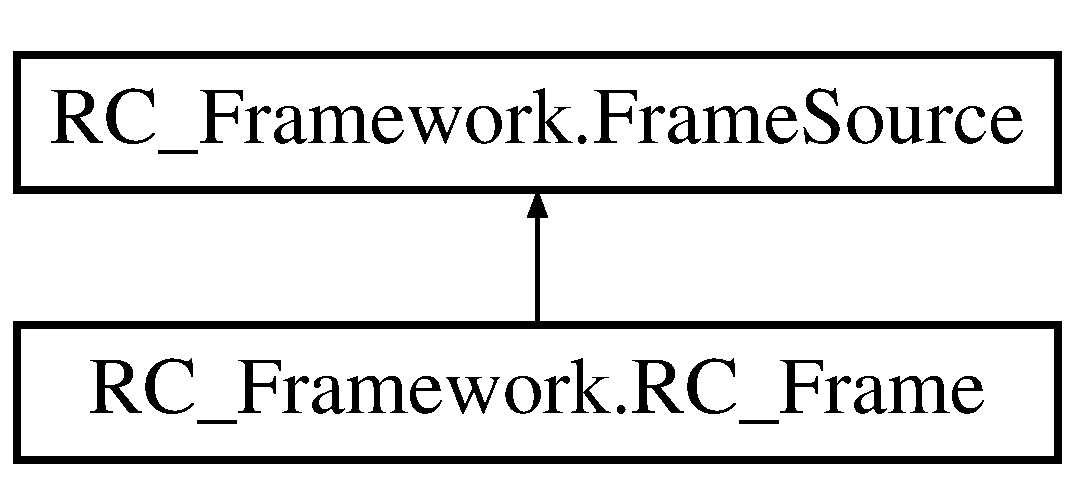
\includegraphics[height=2.000000cm]{class_r_c___framework_1_1_r_c___frame}
\end{center}
\end{figure}
\subsection*{Public Member Functions}
\begin{DoxyCompactItemize}
\item 
\mbox{\hyperlink{class_r_c___framework_1_1_r_c___frame_ac98c117754dc66b735a58067ea2f7f8d}{R\+C\+\_\+\+Frame}} (Rectangle sourceZ, Texture2D texZ)
\begin{DoxyCompactList}\small\item\em constructor \end{DoxyCompactList}\item 
\mbox{\hyperlink{class_r_c___framework_1_1_r_c___frame_a0ffc0dddb25f22ad5ef471848f02005b}{R\+C\+\_\+\+Frame}} (Graphics\+Device gd, string dir, string file\+Name)
\begin{DoxyCompactList}\small\item\em create frame from file \end{DoxyCompactList}\item 
\mbox{\hyperlink{class_r_c___framework_1_1_r_c___frame_a5f7ccf1fe93891b8fff92d76c716ce9e}{R\+C\+\_\+\+Frame}} (\mbox{\hyperlink{class_r_c___framework_1_1_r_c___frame}{R\+C\+\_\+\+Frame}} f)
\begin{DoxyCompactList}\small\item\em copy constructor \end{DoxyCompactList}\item 
override \mbox{\hyperlink{class_r_c___framework_1_1_r_c___frame}{R\+C\+\_\+\+Frame}} \mbox{\hyperlink{class_r_c___framework_1_1_r_c___frame_ad0a2ae1e80157a79713552d9484eb5de}{get\+Frame}} (int num)
\begin{DoxyCompactList}\small\item\em so that a single frame can be a frame source it ignores the frame number (use 0 if it really matters to you) eg get\+Frame(0) \end{DoxyCompactList}\item 
override \mbox{\hyperlink{class_r_c___framework_1_1_r_c___frame}{R\+C\+\_\+\+Frame}} \mbox{\hyperlink{class_r_c___framework_1_1_r_c___frame_a9262ade99ade9dc102aac56587d55d0f}{get\+Frame}} ()
\begin{DoxyCompactList}\small\item\em so that a single frame can be a frame source it ignores the frame number (use 0 if it really matters to you) eg \mbox{\hyperlink{class_r_c___framework_1_1_r_c___frame_a9262ade99ade9dc102aac56587d55d0f}{get\+Frame()}} \end{DoxyCompactList}\item 
void \mbox{\hyperlink{class_r_c___framework_1_1_r_c___frame_a361103a6b92e33f4babc6ec9b02402da}{draw}} (Sprite\+Batch sb, Vector2 pos, Color col)
\begin{DoxyCompactList}\small\item\em draw it at a given 2d loaction \end{DoxyCompactList}\item 
void \mbox{\hyperlink{class_r_c___framework_1_1_r_c___frame_afea32f86d34f1095c53af00e5228622a}{draw}} (Sprite\+Batch sb, Rectangle rect, Color col)
\begin{DoxyCompactList}\small\item\em draw it at a given 2d loaction \end{DoxyCompactList}\end{DoxyCompactItemize}
\subsection*{Public Attributes}
\begin{DoxyCompactItemize}
\item 
Rectangle \mbox{\hyperlink{class_r_c___framework_1_1_r_c___frame_a0e325c29407bc7c18acbbe841095a89a}{source}}
\item 
Texture2D \mbox{\hyperlink{class_r_c___framework_1_1_r_c___frame_a1cf940e9c27e48778d926c5cecea5544}{tex}}
\item 
Rectangle \mbox{\hyperlink{class_r_c___framework_1_1_r_c___frame_a3da33fc90486a672115df3764898b808}{bb}}
\begin{DoxyCompactList}\small\item\em Bounding Box rectange in source pixels x and y are offset from the H\+O\+T\+S\+P\+OT Warning if the hotspot is in the middle of the image/frame then x,y will be negative For users to use (posibbly in update if you need it) currently sprite3 ignores this \end{DoxyCompactList}\item 
Vector2 \mbox{\hyperlink{class_r_c___framework_1_1_r_c___frame_a3188c8af00f675e9419b492d4ef40587}{hot\+Spot\+Offset}}
\begin{DoxyCompactList}\small\item\em hotspot offset x and y from top left corner of either the image -\/ or single frame if its an animation hotspot offet is in pixels in the souce image For users to use (posibbly in update if you need it) currently sprite3 ignores this \end{DoxyCompactList}\end{DoxyCompactItemize}


\subsection{Constructor \& Destructor Documentation}
\mbox{\Hypertarget{class_r_c___framework_1_1_r_c___frame_ac98c117754dc66b735a58067ea2f7f8d}\label{class_r_c___framework_1_1_r_c___frame_ac98c117754dc66b735a58067ea2f7f8d}} 
\index{R\+C\+\_\+\+Framework\+::\+R\+C\+\_\+\+Frame@{R\+C\+\_\+\+Framework\+::\+R\+C\+\_\+\+Frame}!R\+C\+\_\+\+Frame@{R\+C\+\_\+\+Frame}}
\index{R\+C\+\_\+\+Frame@{R\+C\+\_\+\+Frame}!R\+C\+\_\+\+Framework\+::\+R\+C\+\_\+\+Frame@{R\+C\+\_\+\+Framework\+::\+R\+C\+\_\+\+Frame}}
\subsubsection{\texorpdfstring{R\+C\+\_\+\+Frame()}{RC\_Frame()}\hspace{0.1cm}{\footnotesize\ttfamily [1/3]}}
{\footnotesize\ttfamily R\+C\+\_\+\+Framework.\+R\+C\+\_\+\+Frame.\+R\+C\+\_\+\+Frame (\begin{DoxyParamCaption}\item[{Rectangle}]{sourceZ,  }\item[{Texture2D}]{texZ }\end{DoxyParamCaption})}



constructor 


\begin{DoxyParams}{Parameters}
{\em sourceZ} & \\
\hline
{\em texZ} & \\
\hline
\end{DoxyParams}
\mbox{\Hypertarget{class_r_c___framework_1_1_r_c___frame_a0ffc0dddb25f22ad5ef471848f02005b}\label{class_r_c___framework_1_1_r_c___frame_a0ffc0dddb25f22ad5ef471848f02005b}} 
\index{R\+C\+\_\+\+Framework\+::\+R\+C\+\_\+\+Frame@{R\+C\+\_\+\+Framework\+::\+R\+C\+\_\+\+Frame}!R\+C\+\_\+\+Frame@{R\+C\+\_\+\+Frame}}
\index{R\+C\+\_\+\+Frame@{R\+C\+\_\+\+Frame}!R\+C\+\_\+\+Framework\+::\+R\+C\+\_\+\+Frame@{R\+C\+\_\+\+Framework\+::\+R\+C\+\_\+\+Frame}}
\subsubsection{\texorpdfstring{R\+C\+\_\+\+Frame()}{RC\_Frame()}\hspace{0.1cm}{\footnotesize\ttfamily [2/3]}}
{\footnotesize\ttfamily R\+C\+\_\+\+Framework.\+R\+C\+\_\+\+Frame.\+R\+C\+\_\+\+Frame (\begin{DoxyParamCaption}\item[{Graphics\+Device}]{gd,  }\item[{string}]{dir,  }\item[{string}]{file\+Name }\end{DoxyParamCaption})}



create frame from file 


\begin{DoxyParams}{Parameters}
{\em sourceZ} & \\
\hline
{\em texZ} & \\
\hline
\end{DoxyParams}
\mbox{\Hypertarget{class_r_c___framework_1_1_r_c___frame_a5f7ccf1fe93891b8fff92d76c716ce9e}\label{class_r_c___framework_1_1_r_c___frame_a5f7ccf1fe93891b8fff92d76c716ce9e}} 
\index{R\+C\+\_\+\+Framework\+::\+R\+C\+\_\+\+Frame@{R\+C\+\_\+\+Framework\+::\+R\+C\+\_\+\+Frame}!R\+C\+\_\+\+Frame@{R\+C\+\_\+\+Frame}}
\index{R\+C\+\_\+\+Frame@{R\+C\+\_\+\+Frame}!R\+C\+\_\+\+Framework\+::\+R\+C\+\_\+\+Frame@{R\+C\+\_\+\+Framework\+::\+R\+C\+\_\+\+Frame}}
\subsubsection{\texorpdfstring{R\+C\+\_\+\+Frame()}{RC\_Frame()}\hspace{0.1cm}{\footnotesize\ttfamily [3/3]}}
{\footnotesize\ttfamily R\+C\+\_\+\+Framework.\+R\+C\+\_\+\+Frame.\+R\+C\+\_\+\+Frame (\begin{DoxyParamCaption}\item[{\mbox{\hyperlink{class_r_c___framework_1_1_r_c___frame}{R\+C\+\_\+\+Frame}}}]{f }\end{DoxyParamCaption})}



copy constructor 


\begin{DoxyParams}{Parameters}
{\em f} & \\
\hline
\end{DoxyParams}


\subsection{Member Function Documentation}
\mbox{\Hypertarget{class_r_c___framework_1_1_r_c___frame_a361103a6b92e33f4babc6ec9b02402da}\label{class_r_c___framework_1_1_r_c___frame_a361103a6b92e33f4babc6ec9b02402da}} 
\index{R\+C\+\_\+\+Framework\+::\+R\+C\+\_\+\+Frame@{R\+C\+\_\+\+Framework\+::\+R\+C\+\_\+\+Frame}!draw@{draw}}
\index{draw@{draw}!R\+C\+\_\+\+Framework\+::\+R\+C\+\_\+\+Frame@{R\+C\+\_\+\+Framework\+::\+R\+C\+\_\+\+Frame}}
\subsubsection{\texorpdfstring{draw()}{draw()}\hspace{0.1cm}{\footnotesize\ttfamily [1/2]}}
{\footnotesize\ttfamily void R\+C\+\_\+\+Framework.\+R\+C\+\_\+\+Frame.\+draw (\begin{DoxyParamCaption}\item[{Sprite\+Batch}]{sb,  }\item[{Vector2}]{pos,  }\item[{Color}]{col }\end{DoxyParamCaption})}



draw it at a given 2d loaction 


\begin{DoxyParams}{Parameters}
{\em sb} & \\
\hline
{\em pos} & \\
\hline
{\em col} & \\
\hline
\end{DoxyParams}
\mbox{\Hypertarget{class_r_c___framework_1_1_r_c___frame_afea32f86d34f1095c53af00e5228622a}\label{class_r_c___framework_1_1_r_c___frame_afea32f86d34f1095c53af00e5228622a}} 
\index{R\+C\+\_\+\+Framework\+::\+R\+C\+\_\+\+Frame@{R\+C\+\_\+\+Framework\+::\+R\+C\+\_\+\+Frame}!draw@{draw}}
\index{draw@{draw}!R\+C\+\_\+\+Framework\+::\+R\+C\+\_\+\+Frame@{R\+C\+\_\+\+Framework\+::\+R\+C\+\_\+\+Frame}}
\subsubsection{\texorpdfstring{draw()}{draw()}\hspace{0.1cm}{\footnotesize\ttfamily [2/2]}}
{\footnotesize\ttfamily void R\+C\+\_\+\+Framework.\+R\+C\+\_\+\+Frame.\+draw (\begin{DoxyParamCaption}\item[{Sprite\+Batch}]{sb,  }\item[{Rectangle}]{rect,  }\item[{Color}]{col }\end{DoxyParamCaption})}



draw it at a given 2d loaction 


\begin{DoxyParams}{Parameters}
{\em sb} & \\
\hline
{\em pos} & \\
\hline
{\em col} & \\
\hline
\end{DoxyParams}
\mbox{\Hypertarget{class_r_c___framework_1_1_r_c___frame_ad0a2ae1e80157a79713552d9484eb5de}\label{class_r_c___framework_1_1_r_c___frame_ad0a2ae1e80157a79713552d9484eb5de}} 
\index{R\+C\+\_\+\+Framework\+::\+R\+C\+\_\+\+Frame@{R\+C\+\_\+\+Framework\+::\+R\+C\+\_\+\+Frame}!get\+Frame@{get\+Frame}}
\index{get\+Frame@{get\+Frame}!R\+C\+\_\+\+Framework\+::\+R\+C\+\_\+\+Frame@{R\+C\+\_\+\+Framework\+::\+R\+C\+\_\+\+Frame}}
\subsubsection{\texorpdfstring{get\+Frame()}{getFrame()}\hspace{0.1cm}{\footnotesize\ttfamily [1/2]}}
{\footnotesize\ttfamily override \mbox{\hyperlink{class_r_c___framework_1_1_r_c___frame}{R\+C\+\_\+\+Frame}} R\+C\+\_\+\+Framework.\+R\+C\+\_\+\+Frame.\+get\+Frame (\begin{DoxyParamCaption}\item[{int}]{num }\end{DoxyParamCaption})\hspace{0.3cm}{\ttfamily [virtual]}}



so that a single frame can be a frame source it ignores the frame number (use 0 if it really matters to you) eg get\+Frame(0) 


\begin{DoxyParams}{Parameters}
{\em num} & \\
\hline
\end{DoxyParams}
\begin{DoxyReturn}{Returns}

\end{DoxyReturn}


Implements \mbox{\hyperlink{class_r_c___framework_1_1_frame_source_a562dc295b5c265ec760227978802eb3a}{R\+C\+\_\+\+Framework.\+Frame\+Source}}.

\mbox{\Hypertarget{class_r_c___framework_1_1_r_c___frame_a9262ade99ade9dc102aac56587d55d0f}\label{class_r_c___framework_1_1_r_c___frame_a9262ade99ade9dc102aac56587d55d0f}} 
\index{R\+C\+\_\+\+Framework\+::\+R\+C\+\_\+\+Frame@{R\+C\+\_\+\+Framework\+::\+R\+C\+\_\+\+Frame}!get\+Frame@{get\+Frame}}
\index{get\+Frame@{get\+Frame}!R\+C\+\_\+\+Framework\+::\+R\+C\+\_\+\+Frame@{R\+C\+\_\+\+Framework\+::\+R\+C\+\_\+\+Frame}}
\subsubsection{\texorpdfstring{get\+Frame()}{getFrame()}\hspace{0.1cm}{\footnotesize\ttfamily [2/2]}}
{\footnotesize\ttfamily override \mbox{\hyperlink{class_r_c___framework_1_1_r_c___frame}{R\+C\+\_\+\+Frame}} R\+C\+\_\+\+Framework.\+R\+C\+\_\+\+Frame.\+get\+Frame (\begin{DoxyParamCaption}{ }\end{DoxyParamCaption})\hspace{0.3cm}{\ttfamily [virtual]}}



so that a single frame can be a frame source it ignores the frame number (use 0 if it really matters to you) eg \mbox{\hyperlink{class_r_c___framework_1_1_r_c___frame_a9262ade99ade9dc102aac56587d55d0f}{get\+Frame()}} 


\begin{DoxyParams}{Parameters}
{\em num} & \\
\hline
\end{DoxyParams}
\begin{DoxyReturn}{Returns}

\end{DoxyReturn}


Implements \mbox{\hyperlink{class_r_c___framework_1_1_frame_source_a6fd84a8d608da7d9ff2ff5ab10ed4243}{R\+C\+\_\+\+Framework.\+Frame\+Source}}.



\subsection{Member Data Documentation}
\mbox{\Hypertarget{class_r_c___framework_1_1_r_c___frame_a3da33fc90486a672115df3764898b808}\label{class_r_c___framework_1_1_r_c___frame_a3da33fc90486a672115df3764898b808}} 
\index{R\+C\+\_\+\+Framework\+::\+R\+C\+\_\+\+Frame@{R\+C\+\_\+\+Framework\+::\+R\+C\+\_\+\+Frame}!bb@{bb}}
\index{bb@{bb}!R\+C\+\_\+\+Framework\+::\+R\+C\+\_\+\+Frame@{R\+C\+\_\+\+Framework\+::\+R\+C\+\_\+\+Frame}}
\subsubsection{\texorpdfstring{bb}{bb}}
{\footnotesize\ttfamily Rectangle R\+C\+\_\+\+Framework.\+R\+C\+\_\+\+Frame.\+bb}



Bounding Box rectange in source pixels x and y are offset from the H\+O\+T\+S\+P\+OT Warning if the hotspot is in the middle of the image/frame then x,y will be negative For users to use (posibbly in update if you need it) currently sprite3 ignores this 

\mbox{\Hypertarget{class_r_c___framework_1_1_r_c___frame_a3188c8af00f675e9419b492d4ef40587}\label{class_r_c___framework_1_1_r_c___frame_a3188c8af00f675e9419b492d4ef40587}} 
\index{R\+C\+\_\+\+Framework\+::\+R\+C\+\_\+\+Frame@{R\+C\+\_\+\+Framework\+::\+R\+C\+\_\+\+Frame}!hot\+Spot\+Offset@{hot\+Spot\+Offset}}
\index{hot\+Spot\+Offset@{hot\+Spot\+Offset}!R\+C\+\_\+\+Framework\+::\+R\+C\+\_\+\+Frame@{R\+C\+\_\+\+Framework\+::\+R\+C\+\_\+\+Frame}}
\subsubsection{\texorpdfstring{hot\+Spot\+Offset}{hotSpotOffset}}
{\footnotesize\ttfamily Vector2 R\+C\+\_\+\+Framework.\+R\+C\+\_\+\+Frame.\+hot\+Spot\+Offset}



hotspot offset x and y from top left corner of either the image -\/ or single frame if its an animation hotspot offet is in pixels in the souce image For users to use (posibbly in update if you need it) currently sprite3 ignores this 

\mbox{\Hypertarget{class_r_c___framework_1_1_r_c___frame_a0e325c29407bc7c18acbbe841095a89a}\label{class_r_c___framework_1_1_r_c___frame_a0e325c29407bc7c18acbbe841095a89a}} 
\index{R\+C\+\_\+\+Framework\+::\+R\+C\+\_\+\+Frame@{R\+C\+\_\+\+Framework\+::\+R\+C\+\_\+\+Frame}!source@{source}}
\index{source@{source}!R\+C\+\_\+\+Framework\+::\+R\+C\+\_\+\+Frame@{R\+C\+\_\+\+Framework\+::\+R\+C\+\_\+\+Frame}}
\subsubsection{\texorpdfstring{source}{source}}
{\footnotesize\ttfamily Rectangle R\+C\+\_\+\+Framework.\+R\+C\+\_\+\+Frame.\+source}

\mbox{\Hypertarget{class_r_c___framework_1_1_r_c___frame_a1cf940e9c27e48778d926c5cecea5544}\label{class_r_c___framework_1_1_r_c___frame_a1cf940e9c27e48778d926c5cecea5544}} 
\index{R\+C\+\_\+\+Framework\+::\+R\+C\+\_\+\+Frame@{R\+C\+\_\+\+Framework\+::\+R\+C\+\_\+\+Frame}!tex@{tex}}
\index{tex@{tex}!R\+C\+\_\+\+Framework\+::\+R\+C\+\_\+\+Frame@{R\+C\+\_\+\+Framework\+::\+R\+C\+\_\+\+Frame}}
\subsubsection{\texorpdfstring{tex}{tex}}
{\footnotesize\ttfamily Texture2D R\+C\+\_\+\+Framework.\+R\+C\+\_\+\+Frame.\+tex}



The documentation for this class was generated from the following file\+:\begin{DoxyCompactItemize}
\item 
F\+:/\+B/\+R\+C\+\_\+\+Framework2018/\+Source/\mbox{\hyperlink{_r_c___frame_8cs}{R\+C\+\_\+\+Frame.\+cs}}\end{DoxyCompactItemize}

\hypertarget{class_r_c___framework_1_1_r_c___game_state_manager}{}\section{R\+C\+\_\+\+Framework.\+R\+C\+\_\+\+Game\+State\+Manager Class Reference}
\label{class_r_c___framework_1_1_r_c___game_state_manager}\index{R\+C\+\_\+\+Framework.\+R\+C\+\_\+\+Game\+State\+Manager@{R\+C\+\_\+\+Framework.\+R\+C\+\_\+\+Game\+State\+Manager}}


To manage levels ~\newline
 


\subsection*{Public Member Functions}
\begin{DoxyCompactItemize}
\item 
\mbox{\hyperlink{class_r_c___framework_1_1_r_c___game_state_manager_a481a415ee368710463d773ecffc69a26}{R\+C\+\_\+\+Game\+State\+Manager}} ()
\item 
void \mbox{\hyperlink{class_r_c___framework_1_1_r_c___game_state_manager_abc201bbd33d01162573ae56bb8821532}{Add\+Level}} (int lev\+Num, \mbox{\hyperlink{class_r_c___framework_1_1_r_c___game_state_parent}{R\+C\+\_\+\+Game\+State\+Parent}} lev)
\item 
\mbox{\hyperlink{class_r_c___framework_1_1_r_c___game_state_parent}{R\+C\+\_\+\+Game\+State\+Parent}} \mbox{\hyperlink{class_r_c___framework_1_1_r_c___game_state_manager_a6e4402df19c3f71484c99a79465776a9}{get\+Level}} (int lev\+Num)
\item 
void \mbox{\hyperlink{class_r_c___framework_1_1_r_c___game_state_manager_abc013de4037dfb71de3c641370bf95e1}{set\+Level}} (int lev\+Num)
\item 
void \mbox{\hyperlink{class_r_c___framework_1_1_r_c___game_state_manager_a608feb785ba1237cd73e4d923ba0c984}{push\+Level}} (int lev\+Num)
\item 
int \mbox{\hyperlink{class_r_c___framework_1_1_r_c___game_state_manager_a6f0a705a4cf67f540c8b3b6b05ebf908}{pop\+Level}} ()
\item 
void \mbox{\hyperlink{class_r_c___framework_1_1_r_c___game_state_manager_aa499f3ee8c7b4e013039ef9a895b7bff}{set\+Empty\+Level}} ()
\item 
\mbox{\hyperlink{class_r_c___framework_1_1_r_c___game_state_parent}{R\+C\+\_\+\+Game\+State\+Parent}} \mbox{\hyperlink{class_r_c___framework_1_1_r_c___game_state_manager_a5f86142eb931e571ae1116d8be88bcab}{get\+Current\+Level}} ()
\item 
int \mbox{\hyperlink{class_r_c___framework_1_1_r_c___game_state_manager_ada1ef603c6e9c1d7d40977500e4191d3}{get\+Current\+Level\+Num}} ()
\end{DoxyCompactItemize}
\subsection*{Public Attributes}
\begin{DoxyCompactItemize}
\item 
\mbox{\hyperlink{class_r_c___framework_1_1_r_c___game_state_parent}{R\+C\+\_\+\+Game\+State\+Parent}} \mbox{\hyperlink{class_r_c___framework_1_1_r_c___game_state_manager_a36d7fc859f13ad252673c0fae038c8b7}{prev\+State\+Play\+Level}} =null
\end{DoxyCompactItemize}


\subsection{Detailed Description}
To manage levels ~\newline




\subsection{Constructor \& Destructor Documentation}
\mbox{\Hypertarget{class_r_c___framework_1_1_r_c___game_state_manager_a481a415ee368710463d773ecffc69a26}\label{class_r_c___framework_1_1_r_c___game_state_manager_a481a415ee368710463d773ecffc69a26}} 
\index{R\+C\+\_\+\+Framework\+::\+R\+C\+\_\+\+Game\+State\+Manager@{R\+C\+\_\+\+Framework\+::\+R\+C\+\_\+\+Game\+State\+Manager}!R\+C\+\_\+\+Game\+State\+Manager@{R\+C\+\_\+\+Game\+State\+Manager}}
\index{R\+C\+\_\+\+Game\+State\+Manager@{R\+C\+\_\+\+Game\+State\+Manager}!R\+C\+\_\+\+Framework\+::\+R\+C\+\_\+\+Game\+State\+Manager@{R\+C\+\_\+\+Framework\+::\+R\+C\+\_\+\+Game\+State\+Manager}}
\subsubsection{\texorpdfstring{R\+C\+\_\+\+Game\+State\+Manager()}{RC\_GameStateManager()}}
{\footnotesize\ttfamily R\+C\+\_\+\+Framework.\+R\+C\+\_\+\+Game\+State\+Manager.\+R\+C\+\_\+\+Game\+State\+Manager (\begin{DoxyParamCaption}{ }\end{DoxyParamCaption})}



\subsection{Member Function Documentation}
\mbox{\Hypertarget{class_r_c___framework_1_1_r_c___game_state_manager_abc201bbd33d01162573ae56bb8821532}\label{class_r_c___framework_1_1_r_c___game_state_manager_abc201bbd33d01162573ae56bb8821532}} 
\index{R\+C\+\_\+\+Framework\+::\+R\+C\+\_\+\+Game\+State\+Manager@{R\+C\+\_\+\+Framework\+::\+R\+C\+\_\+\+Game\+State\+Manager}!Add\+Level@{Add\+Level}}
\index{Add\+Level@{Add\+Level}!R\+C\+\_\+\+Framework\+::\+R\+C\+\_\+\+Game\+State\+Manager@{R\+C\+\_\+\+Framework\+::\+R\+C\+\_\+\+Game\+State\+Manager}}
\subsubsection{\texorpdfstring{Add\+Level()}{AddLevel()}}
{\footnotesize\ttfamily void R\+C\+\_\+\+Framework.\+R\+C\+\_\+\+Game\+State\+Manager.\+Add\+Level (\begin{DoxyParamCaption}\item[{int}]{lev\+Num,  }\item[{\mbox{\hyperlink{class_r_c___framework_1_1_r_c___game_state_parent}{R\+C\+\_\+\+Game\+State\+Parent}}}]{lev }\end{DoxyParamCaption})}

\mbox{\Hypertarget{class_r_c___framework_1_1_r_c___game_state_manager_a5f86142eb931e571ae1116d8be88bcab}\label{class_r_c___framework_1_1_r_c___game_state_manager_a5f86142eb931e571ae1116d8be88bcab}} 
\index{R\+C\+\_\+\+Framework\+::\+R\+C\+\_\+\+Game\+State\+Manager@{R\+C\+\_\+\+Framework\+::\+R\+C\+\_\+\+Game\+State\+Manager}!get\+Current\+Level@{get\+Current\+Level}}
\index{get\+Current\+Level@{get\+Current\+Level}!R\+C\+\_\+\+Framework\+::\+R\+C\+\_\+\+Game\+State\+Manager@{R\+C\+\_\+\+Framework\+::\+R\+C\+\_\+\+Game\+State\+Manager}}
\subsubsection{\texorpdfstring{get\+Current\+Level()}{getCurrentLevel()}}
{\footnotesize\ttfamily \mbox{\hyperlink{class_r_c___framework_1_1_r_c___game_state_parent}{R\+C\+\_\+\+Game\+State\+Parent}} R\+C\+\_\+\+Framework.\+R\+C\+\_\+\+Game\+State\+Manager.\+get\+Current\+Level (\begin{DoxyParamCaption}{ }\end{DoxyParamCaption})}

\mbox{\Hypertarget{class_r_c___framework_1_1_r_c___game_state_manager_ada1ef603c6e9c1d7d40977500e4191d3}\label{class_r_c___framework_1_1_r_c___game_state_manager_ada1ef603c6e9c1d7d40977500e4191d3}} 
\index{R\+C\+\_\+\+Framework\+::\+R\+C\+\_\+\+Game\+State\+Manager@{R\+C\+\_\+\+Framework\+::\+R\+C\+\_\+\+Game\+State\+Manager}!get\+Current\+Level\+Num@{get\+Current\+Level\+Num}}
\index{get\+Current\+Level\+Num@{get\+Current\+Level\+Num}!R\+C\+\_\+\+Framework\+::\+R\+C\+\_\+\+Game\+State\+Manager@{R\+C\+\_\+\+Framework\+::\+R\+C\+\_\+\+Game\+State\+Manager}}
\subsubsection{\texorpdfstring{get\+Current\+Level\+Num()}{getCurrentLevelNum()}}
{\footnotesize\ttfamily int R\+C\+\_\+\+Framework.\+R\+C\+\_\+\+Game\+State\+Manager.\+get\+Current\+Level\+Num (\begin{DoxyParamCaption}{ }\end{DoxyParamCaption})}

\mbox{\Hypertarget{class_r_c___framework_1_1_r_c___game_state_manager_a6e4402df19c3f71484c99a79465776a9}\label{class_r_c___framework_1_1_r_c___game_state_manager_a6e4402df19c3f71484c99a79465776a9}} 
\index{R\+C\+\_\+\+Framework\+::\+R\+C\+\_\+\+Game\+State\+Manager@{R\+C\+\_\+\+Framework\+::\+R\+C\+\_\+\+Game\+State\+Manager}!get\+Level@{get\+Level}}
\index{get\+Level@{get\+Level}!R\+C\+\_\+\+Framework\+::\+R\+C\+\_\+\+Game\+State\+Manager@{R\+C\+\_\+\+Framework\+::\+R\+C\+\_\+\+Game\+State\+Manager}}
\subsubsection{\texorpdfstring{get\+Level()}{getLevel()}}
{\footnotesize\ttfamily \mbox{\hyperlink{class_r_c___framework_1_1_r_c___game_state_parent}{R\+C\+\_\+\+Game\+State\+Parent}} R\+C\+\_\+\+Framework.\+R\+C\+\_\+\+Game\+State\+Manager.\+get\+Level (\begin{DoxyParamCaption}\item[{int}]{lev\+Num }\end{DoxyParamCaption})}

\mbox{\Hypertarget{class_r_c___framework_1_1_r_c___game_state_manager_a6f0a705a4cf67f540c8b3b6b05ebf908}\label{class_r_c___framework_1_1_r_c___game_state_manager_a6f0a705a4cf67f540c8b3b6b05ebf908}} 
\index{R\+C\+\_\+\+Framework\+::\+R\+C\+\_\+\+Game\+State\+Manager@{R\+C\+\_\+\+Framework\+::\+R\+C\+\_\+\+Game\+State\+Manager}!pop\+Level@{pop\+Level}}
\index{pop\+Level@{pop\+Level}!R\+C\+\_\+\+Framework\+::\+R\+C\+\_\+\+Game\+State\+Manager@{R\+C\+\_\+\+Framework\+::\+R\+C\+\_\+\+Game\+State\+Manager}}
\subsubsection{\texorpdfstring{pop\+Level()}{popLevel()}}
{\footnotesize\ttfamily int R\+C\+\_\+\+Framework.\+R\+C\+\_\+\+Game\+State\+Manager.\+pop\+Level (\begin{DoxyParamCaption}{ }\end{DoxyParamCaption})}

\mbox{\Hypertarget{class_r_c___framework_1_1_r_c___game_state_manager_a608feb785ba1237cd73e4d923ba0c984}\label{class_r_c___framework_1_1_r_c___game_state_manager_a608feb785ba1237cd73e4d923ba0c984}} 
\index{R\+C\+\_\+\+Framework\+::\+R\+C\+\_\+\+Game\+State\+Manager@{R\+C\+\_\+\+Framework\+::\+R\+C\+\_\+\+Game\+State\+Manager}!push\+Level@{push\+Level}}
\index{push\+Level@{push\+Level}!R\+C\+\_\+\+Framework\+::\+R\+C\+\_\+\+Game\+State\+Manager@{R\+C\+\_\+\+Framework\+::\+R\+C\+\_\+\+Game\+State\+Manager}}
\subsubsection{\texorpdfstring{push\+Level()}{pushLevel()}}
{\footnotesize\ttfamily void R\+C\+\_\+\+Framework.\+R\+C\+\_\+\+Game\+State\+Manager.\+push\+Level (\begin{DoxyParamCaption}\item[{int}]{lev\+Num }\end{DoxyParamCaption})}

\mbox{\Hypertarget{class_r_c___framework_1_1_r_c___game_state_manager_aa499f3ee8c7b4e013039ef9a895b7bff}\label{class_r_c___framework_1_1_r_c___game_state_manager_aa499f3ee8c7b4e013039ef9a895b7bff}} 
\index{R\+C\+\_\+\+Framework\+::\+R\+C\+\_\+\+Game\+State\+Manager@{R\+C\+\_\+\+Framework\+::\+R\+C\+\_\+\+Game\+State\+Manager}!set\+Empty\+Level@{set\+Empty\+Level}}
\index{set\+Empty\+Level@{set\+Empty\+Level}!R\+C\+\_\+\+Framework\+::\+R\+C\+\_\+\+Game\+State\+Manager@{R\+C\+\_\+\+Framework\+::\+R\+C\+\_\+\+Game\+State\+Manager}}
\subsubsection{\texorpdfstring{set\+Empty\+Level()}{setEmptyLevel()}}
{\footnotesize\ttfamily void R\+C\+\_\+\+Framework.\+R\+C\+\_\+\+Game\+State\+Manager.\+set\+Empty\+Level (\begin{DoxyParamCaption}{ }\end{DoxyParamCaption})}

\mbox{\Hypertarget{class_r_c___framework_1_1_r_c___game_state_manager_abc013de4037dfb71de3c641370bf95e1}\label{class_r_c___framework_1_1_r_c___game_state_manager_abc013de4037dfb71de3c641370bf95e1}} 
\index{R\+C\+\_\+\+Framework\+::\+R\+C\+\_\+\+Game\+State\+Manager@{R\+C\+\_\+\+Framework\+::\+R\+C\+\_\+\+Game\+State\+Manager}!set\+Level@{set\+Level}}
\index{set\+Level@{set\+Level}!R\+C\+\_\+\+Framework\+::\+R\+C\+\_\+\+Game\+State\+Manager@{R\+C\+\_\+\+Framework\+::\+R\+C\+\_\+\+Game\+State\+Manager}}
\subsubsection{\texorpdfstring{set\+Level()}{setLevel()}}
{\footnotesize\ttfamily void R\+C\+\_\+\+Framework.\+R\+C\+\_\+\+Game\+State\+Manager.\+set\+Level (\begin{DoxyParamCaption}\item[{int}]{lev\+Num }\end{DoxyParamCaption})}



\subsection{Member Data Documentation}
\mbox{\Hypertarget{class_r_c___framework_1_1_r_c___game_state_manager_a36d7fc859f13ad252673c0fae038c8b7}\label{class_r_c___framework_1_1_r_c___game_state_manager_a36d7fc859f13ad252673c0fae038c8b7}} 
\index{R\+C\+\_\+\+Framework\+::\+R\+C\+\_\+\+Game\+State\+Manager@{R\+C\+\_\+\+Framework\+::\+R\+C\+\_\+\+Game\+State\+Manager}!prev\+State\+Play\+Level@{prev\+State\+Play\+Level}}
\index{prev\+State\+Play\+Level@{prev\+State\+Play\+Level}!R\+C\+\_\+\+Framework\+::\+R\+C\+\_\+\+Game\+State\+Manager@{R\+C\+\_\+\+Framework\+::\+R\+C\+\_\+\+Game\+State\+Manager}}
\subsubsection{\texorpdfstring{prev\+State\+Play\+Level}{prevStatePlayLevel}}
{\footnotesize\ttfamily \mbox{\hyperlink{class_r_c___framework_1_1_r_c___game_state_parent}{R\+C\+\_\+\+Game\+State\+Parent}} R\+C\+\_\+\+Framework.\+R\+C\+\_\+\+Game\+State\+Manager.\+prev\+State\+Play\+Level =null}



The documentation for this class was generated from the following file\+:\begin{DoxyCompactItemize}
\item 
F\+:/\+B/\+R\+C\+\_\+\+Framework2018/\+Source/\mbox{\hyperlink{_r_c___game_state_8cs}{R\+C\+\_\+\+Game\+State.\+cs}}\end{DoxyCompactItemize}

\hypertarget{class_r_c___framework_1_1_r_c___game_state_parent}{}\section{R\+C\+\_\+\+Framework.\+R\+C\+\_\+\+Game\+State\+Parent Class Reference}
\label{class_r_c___framework_1_1_r_c___game_state_parent}\index{R\+C\+\_\+\+Framework.\+R\+C\+\_\+\+Game\+State\+Parent@{R\+C\+\_\+\+Framework.\+R\+C\+\_\+\+Game\+State\+Parent}}


Parent Stagre class all levels inherit from this  


Inheritance diagram for R\+C\+\_\+\+Framework.\+R\+C\+\_\+\+Game\+State\+Parent\+:\begin{figure}[H]
\begin{center}
\leavevmode
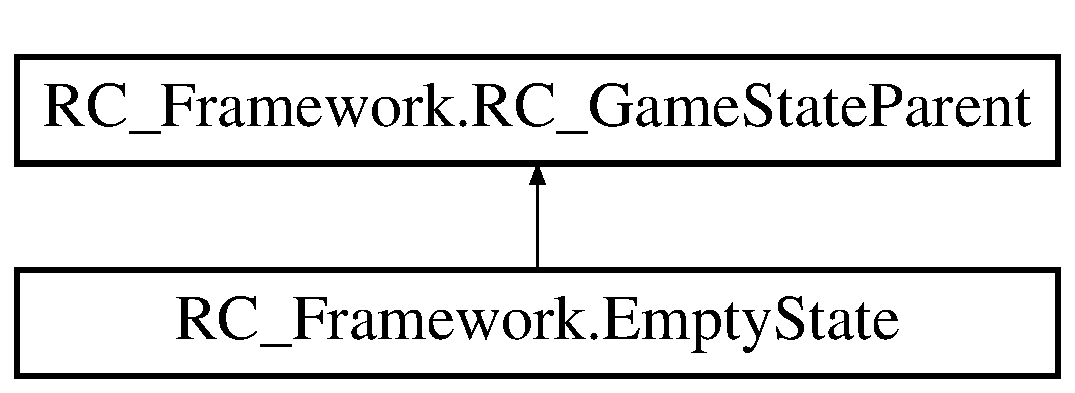
\includegraphics[height=2.000000cm]{class_r_c___framework_1_1_r_c___game_state_parent}
\end{center}
\end{figure}
\subsection*{Public Member Functions}
\begin{DoxyCompactItemize}
\item 
virtual void \mbox{\hyperlink{class_r_c___framework_1_1_r_c___game_state_parent_a3fd47a4805f19683bc68eb3e20f36086}{Initialize\+Level}} (Graphics\+Device g, Sprite\+Batch s, Content\+Manager c, \mbox{\hyperlink{class_r_c___framework_1_1_r_c___game_state_manager}{R\+C\+\_\+\+Game\+State\+Manager}} lm)
\item 
virtual void \mbox{\hyperlink{class_r_c___framework_1_1_r_c___game_state_parent_a6c87e9eecbd5ac046fd1987ea09da716}{Load\+Content}} ()
\item 
virtual void \mbox{\hyperlink{class_r_c___framework_1_1_r_c___game_state_parent_a7752d80f5d187c87f85ec6a2c38b2dc1}{Unload\+Content}} ()
\item 
virtual void \mbox{\hyperlink{class_r_c___framework_1_1_r_c___game_state_parent_a99f481185124bd50d92a032416e96d7a}{Enter\+Level}} (int from\+Level\+Num)
\item 
virtual void \mbox{\hyperlink{class_r_c___framework_1_1_r_c___game_state_parent_a1501d4293365e35c42a659a7d7477fc7}{Exit\+Level}} ()
\item 
virtual void \mbox{\hyperlink{class_r_c___framework_1_1_r_c___game_state_parent_af276a58dd0a0581095a2776801942860}{Update}} (Game\+Time game\+Time)
\item 
abstract void \mbox{\hyperlink{class_r_c___framework_1_1_r_c___game_state_parent_adec421bc58a381ab34ffa74b495fa3c9}{Draw}} (Game\+Time game\+Time)
\end{DoxyCompactItemize}
\subsection*{Static Public Member Functions}
\begin{DoxyCompactItemize}
\item 
static void \mbox{\hyperlink{class_r_c___framework_1_1_r_c___game_state_parent_a97c7dff53d0c3543e8ea01fcdb2cd1de}{get\+Keyboard\+And\+Mouse}} ()
\begin{DoxyCompactList}\small\item\em Utility routine to set up keyboard and mouse \end{DoxyCompactList}\end{DoxyCompactItemize}
\subsection*{Static Public Attributes}
\begin{DoxyCompactItemize}
\item 
static Graphics\+Device \mbox{\hyperlink{class_r_c___framework_1_1_r_c___game_state_parent_afd2f2ef0999c284adc241563b5c6314a}{graphics\+Device}}
\item 
static Sprite\+Batch \mbox{\hyperlink{class_r_c___framework_1_1_r_c___game_state_parent_a53d22435d3ccf01092a06e83873a9eeb}{sprite\+Batch}}
\item 
static Content\+Manager \mbox{\hyperlink{class_r_c___framework_1_1_r_c___game_state_parent_a772dfa1ba0878142104adfc3eae559e5}{Content}}
\item 
static \mbox{\hyperlink{class_r_c___framework_1_1_r_c___game_state_manager}{R\+C\+\_\+\+Game\+State\+Manager}} \mbox{\hyperlink{class_r_c___framework_1_1_r_c___game_state_parent_a3511187c06d875b45ff212506147cb3d}{game\+State\+Manager}}
\item 
static Keyboard\+State \mbox{\hyperlink{class_r_c___framework_1_1_r_c___game_state_parent_ad06a8d6e2406a9dc1d8300c8dc71f29a}{key\+State}}
\item 
static Keyboard\+State \mbox{\hyperlink{class_r_c___framework_1_1_r_c___game_state_parent_a55d41a359519fd898e465887b452063d}{prev\+Key\+State}}
\item 
static float \mbox{\hyperlink{class_r_c___framework_1_1_r_c___game_state_parent_af534866f8d4fa277ffacce36c161da65}{mouse\+\_\+x}} = 0
\item 
static float \mbox{\hyperlink{class_r_c___framework_1_1_r_c___game_state_parent_ac8ccd45ec22dd583f59d8d21663abe97}{mouse\+\_\+y}} = 0
\item 
static Mouse\+State \mbox{\hyperlink{class_r_c___framework_1_1_r_c___game_state_parent_a4009cee63013baddd6c472493878c631}{current\+Mouse\+State}}
\item 
static Mouse\+State \mbox{\hyperlink{class_r_c___framework_1_1_r_c___game_state_parent_a867cec9b3490d334194932d82e5ea6c0}{previous\+Mouse\+State}}
\item 
static Sprite\+Font \mbox{\hyperlink{class_r_c___framework_1_1_r_c___game_state_parent_a0e2ab0c92858466e1628dc79ef237a8b}{font1}}
\end{DoxyCompactItemize}


\subsection{Detailed Description}
Parent Stagre class all levels inherit from this 



\subsection{Member Function Documentation}
\mbox{\Hypertarget{class_r_c___framework_1_1_r_c___game_state_parent_adec421bc58a381ab34ffa74b495fa3c9}\label{class_r_c___framework_1_1_r_c___game_state_parent_adec421bc58a381ab34ffa74b495fa3c9}} 
\index{R\+C\+\_\+\+Framework\+::\+R\+C\+\_\+\+Game\+State\+Parent@{R\+C\+\_\+\+Framework\+::\+R\+C\+\_\+\+Game\+State\+Parent}!Draw@{Draw}}
\index{Draw@{Draw}!R\+C\+\_\+\+Framework\+::\+R\+C\+\_\+\+Game\+State\+Parent@{R\+C\+\_\+\+Framework\+::\+R\+C\+\_\+\+Game\+State\+Parent}}
\subsubsection{\texorpdfstring{Draw()}{Draw()}}
{\footnotesize\ttfamily abstract void R\+C\+\_\+\+Framework.\+R\+C\+\_\+\+Game\+State\+Parent.\+Draw (\begin{DoxyParamCaption}\item[{Game\+Time}]{game\+Time }\end{DoxyParamCaption})\hspace{0.3cm}{\ttfamily [pure virtual]}}



Implemented in \mbox{\hyperlink{class_r_c___framework_1_1_empty_state_adfa60e364416dfe5f9a3ba565bc6329b}{R\+C\+\_\+\+Framework.\+Empty\+State}}.

\mbox{\Hypertarget{class_r_c___framework_1_1_r_c___game_state_parent_a99f481185124bd50d92a032416e96d7a}\label{class_r_c___framework_1_1_r_c___game_state_parent_a99f481185124bd50d92a032416e96d7a}} 
\index{R\+C\+\_\+\+Framework\+::\+R\+C\+\_\+\+Game\+State\+Parent@{R\+C\+\_\+\+Framework\+::\+R\+C\+\_\+\+Game\+State\+Parent}!Enter\+Level@{Enter\+Level}}
\index{Enter\+Level@{Enter\+Level}!R\+C\+\_\+\+Framework\+::\+R\+C\+\_\+\+Game\+State\+Parent@{R\+C\+\_\+\+Framework\+::\+R\+C\+\_\+\+Game\+State\+Parent}}
\subsubsection{\texorpdfstring{Enter\+Level()}{EnterLevel()}}
{\footnotesize\ttfamily virtual void R\+C\+\_\+\+Framework.\+R\+C\+\_\+\+Game\+State\+Parent.\+Enter\+Level (\begin{DoxyParamCaption}\item[{int}]{from\+Level\+Num }\end{DoxyParamCaption})\hspace{0.3cm}{\ttfamily [virtual]}}

\mbox{\Hypertarget{class_r_c___framework_1_1_r_c___game_state_parent_a1501d4293365e35c42a659a7d7477fc7}\label{class_r_c___framework_1_1_r_c___game_state_parent_a1501d4293365e35c42a659a7d7477fc7}} 
\index{R\+C\+\_\+\+Framework\+::\+R\+C\+\_\+\+Game\+State\+Parent@{R\+C\+\_\+\+Framework\+::\+R\+C\+\_\+\+Game\+State\+Parent}!Exit\+Level@{Exit\+Level}}
\index{Exit\+Level@{Exit\+Level}!R\+C\+\_\+\+Framework\+::\+R\+C\+\_\+\+Game\+State\+Parent@{R\+C\+\_\+\+Framework\+::\+R\+C\+\_\+\+Game\+State\+Parent}}
\subsubsection{\texorpdfstring{Exit\+Level()}{ExitLevel()}}
{\footnotesize\ttfamily virtual void R\+C\+\_\+\+Framework.\+R\+C\+\_\+\+Game\+State\+Parent.\+Exit\+Level (\begin{DoxyParamCaption}{ }\end{DoxyParamCaption})\hspace{0.3cm}{\ttfamily [virtual]}}

\mbox{\Hypertarget{class_r_c___framework_1_1_r_c___game_state_parent_a97c7dff53d0c3543e8ea01fcdb2cd1de}\label{class_r_c___framework_1_1_r_c___game_state_parent_a97c7dff53d0c3543e8ea01fcdb2cd1de}} 
\index{R\+C\+\_\+\+Framework\+::\+R\+C\+\_\+\+Game\+State\+Parent@{R\+C\+\_\+\+Framework\+::\+R\+C\+\_\+\+Game\+State\+Parent}!get\+Keyboard\+And\+Mouse@{get\+Keyboard\+And\+Mouse}}
\index{get\+Keyboard\+And\+Mouse@{get\+Keyboard\+And\+Mouse}!R\+C\+\_\+\+Framework\+::\+R\+C\+\_\+\+Game\+State\+Parent@{R\+C\+\_\+\+Framework\+::\+R\+C\+\_\+\+Game\+State\+Parent}}
\subsubsection{\texorpdfstring{get\+Keyboard\+And\+Mouse()}{getKeyboardAndMouse()}}
{\footnotesize\ttfamily static void R\+C\+\_\+\+Framework.\+R\+C\+\_\+\+Game\+State\+Parent.\+get\+Keyboard\+And\+Mouse (\begin{DoxyParamCaption}{ }\end{DoxyParamCaption})\hspace{0.3cm}{\ttfamily [static]}}



Utility routine to set up keyboard and mouse 

\mbox{\Hypertarget{class_r_c___framework_1_1_r_c___game_state_parent_a3fd47a4805f19683bc68eb3e20f36086}\label{class_r_c___framework_1_1_r_c___game_state_parent_a3fd47a4805f19683bc68eb3e20f36086}} 
\index{R\+C\+\_\+\+Framework\+::\+R\+C\+\_\+\+Game\+State\+Parent@{R\+C\+\_\+\+Framework\+::\+R\+C\+\_\+\+Game\+State\+Parent}!Initialize\+Level@{Initialize\+Level}}
\index{Initialize\+Level@{Initialize\+Level}!R\+C\+\_\+\+Framework\+::\+R\+C\+\_\+\+Game\+State\+Parent@{R\+C\+\_\+\+Framework\+::\+R\+C\+\_\+\+Game\+State\+Parent}}
\subsubsection{\texorpdfstring{Initialize\+Level()}{InitializeLevel()}}
{\footnotesize\ttfamily virtual void R\+C\+\_\+\+Framework.\+R\+C\+\_\+\+Game\+State\+Parent.\+Initialize\+Level (\begin{DoxyParamCaption}\item[{Graphics\+Device}]{g,  }\item[{Sprite\+Batch}]{s,  }\item[{Content\+Manager}]{c,  }\item[{\mbox{\hyperlink{class_r_c___framework_1_1_r_c___game_state_manager}{R\+C\+\_\+\+Game\+State\+Manager}}}]{lm }\end{DoxyParamCaption})\hspace{0.3cm}{\ttfamily [virtual]}}

\mbox{\Hypertarget{class_r_c___framework_1_1_r_c___game_state_parent_a6c87e9eecbd5ac046fd1987ea09da716}\label{class_r_c___framework_1_1_r_c___game_state_parent_a6c87e9eecbd5ac046fd1987ea09da716}} 
\index{R\+C\+\_\+\+Framework\+::\+R\+C\+\_\+\+Game\+State\+Parent@{R\+C\+\_\+\+Framework\+::\+R\+C\+\_\+\+Game\+State\+Parent}!Load\+Content@{Load\+Content}}
\index{Load\+Content@{Load\+Content}!R\+C\+\_\+\+Framework\+::\+R\+C\+\_\+\+Game\+State\+Parent@{R\+C\+\_\+\+Framework\+::\+R\+C\+\_\+\+Game\+State\+Parent}}
\subsubsection{\texorpdfstring{Load\+Content()}{LoadContent()}}
{\footnotesize\ttfamily virtual void R\+C\+\_\+\+Framework.\+R\+C\+\_\+\+Game\+State\+Parent.\+Load\+Content (\begin{DoxyParamCaption}{ }\end{DoxyParamCaption})\hspace{0.3cm}{\ttfamily [virtual]}}

\mbox{\Hypertarget{class_r_c___framework_1_1_r_c___game_state_parent_a7752d80f5d187c87f85ec6a2c38b2dc1}\label{class_r_c___framework_1_1_r_c___game_state_parent_a7752d80f5d187c87f85ec6a2c38b2dc1}} 
\index{R\+C\+\_\+\+Framework\+::\+R\+C\+\_\+\+Game\+State\+Parent@{R\+C\+\_\+\+Framework\+::\+R\+C\+\_\+\+Game\+State\+Parent}!Unload\+Content@{Unload\+Content}}
\index{Unload\+Content@{Unload\+Content}!R\+C\+\_\+\+Framework\+::\+R\+C\+\_\+\+Game\+State\+Parent@{R\+C\+\_\+\+Framework\+::\+R\+C\+\_\+\+Game\+State\+Parent}}
\subsubsection{\texorpdfstring{Unload\+Content()}{UnloadContent()}}
{\footnotesize\ttfamily virtual void R\+C\+\_\+\+Framework.\+R\+C\+\_\+\+Game\+State\+Parent.\+Unload\+Content (\begin{DoxyParamCaption}{ }\end{DoxyParamCaption})\hspace{0.3cm}{\ttfamily [virtual]}}

\mbox{\Hypertarget{class_r_c___framework_1_1_r_c___game_state_parent_af276a58dd0a0581095a2776801942860}\label{class_r_c___framework_1_1_r_c___game_state_parent_af276a58dd0a0581095a2776801942860}} 
\index{R\+C\+\_\+\+Framework\+::\+R\+C\+\_\+\+Game\+State\+Parent@{R\+C\+\_\+\+Framework\+::\+R\+C\+\_\+\+Game\+State\+Parent}!Update@{Update}}
\index{Update@{Update}!R\+C\+\_\+\+Framework\+::\+R\+C\+\_\+\+Game\+State\+Parent@{R\+C\+\_\+\+Framework\+::\+R\+C\+\_\+\+Game\+State\+Parent}}
\subsubsection{\texorpdfstring{Update()}{Update()}}
{\footnotesize\ttfamily virtual void R\+C\+\_\+\+Framework.\+R\+C\+\_\+\+Game\+State\+Parent.\+Update (\begin{DoxyParamCaption}\item[{Game\+Time}]{game\+Time }\end{DoxyParamCaption})\hspace{0.3cm}{\ttfamily [virtual]}}



\subsection{Member Data Documentation}
\mbox{\Hypertarget{class_r_c___framework_1_1_r_c___game_state_parent_a772dfa1ba0878142104adfc3eae559e5}\label{class_r_c___framework_1_1_r_c___game_state_parent_a772dfa1ba0878142104adfc3eae559e5}} 
\index{R\+C\+\_\+\+Framework\+::\+R\+C\+\_\+\+Game\+State\+Parent@{R\+C\+\_\+\+Framework\+::\+R\+C\+\_\+\+Game\+State\+Parent}!Content@{Content}}
\index{Content@{Content}!R\+C\+\_\+\+Framework\+::\+R\+C\+\_\+\+Game\+State\+Parent@{R\+C\+\_\+\+Framework\+::\+R\+C\+\_\+\+Game\+State\+Parent}}
\subsubsection{\texorpdfstring{Content}{Content}}
{\footnotesize\ttfamily Content\+Manager R\+C\+\_\+\+Framework.\+R\+C\+\_\+\+Game\+State\+Parent.\+Content\hspace{0.3cm}{\ttfamily [static]}}

\mbox{\Hypertarget{class_r_c___framework_1_1_r_c___game_state_parent_a4009cee63013baddd6c472493878c631}\label{class_r_c___framework_1_1_r_c___game_state_parent_a4009cee63013baddd6c472493878c631}} 
\index{R\+C\+\_\+\+Framework\+::\+R\+C\+\_\+\+Game\+State\+Parent@{R\+C\+\_\+\+Framework\+::\+R\+C\+\_\+\+Game\+State\+Parent}!current\+Mouse\+State@{current\+Mouse\+State}}
\index{current\+Mouse\+State@{current\+Mouse\+State}!R\+C\+\_\+\+Framework\+::\+R\+C\+\_\+\+Game\+State\+Parent@{R\+C\+\_\+\+Framework\+::\+R\+C\+\_\+\+Game\+State\+Parent}}
\subsubsection{\texorpdfstring{current\+Mouse\+State}{currentMouseState}}
{\footnotesize\ttfamily Mouse\+State R\+C\+\_\+\+Framework.\+R\+C\+\_\+\+Game\+State\+Parent.\+current\+Mouse\+State\hspace{0.3cm}{\ttfamily [static]}}

\mbox{\Hypertarget{class_r_c___framework_1_1_r_c___game_state_parent_a0e2ab0c92858466e1628dc79ef237a8b}\label{class_r_c___framework_1_1_r_c___game_state_parent_a0e2ab0c92858466e1628dc79ef237a8b}} 
\index{R\+C\+\_\+\+Framework\+::\+R\+C\+\_\+\+Game\+State\+Parent@{R\+C\+\_\+\+Framework\+::\+R\+C\+\_\+\+Game\+State\+Parent}!font1@{font1}}
\index{font1@{font1}!R\+C\+\_\+\+Framework\+::\+R\+C\+\_\+\+Game\+State\+Parent@{R\+C\+\_\+\+Framework\+::\+R\+C\+\_\+\+Game\+State\+Parent}}
\subsubsection{\texorpdfstring{font1}{font1}}
{\footnotesize\ttfamily Sprite\+Font R\+C\+\_\+\+Framework.\+R\+C\+\_\+\+Game\+State\+Parent.\+font1\hspace{0.3cm}{\ttfamily [static]}}

\mbox{\Hypertarget{class_r_c___framework_1_1_r_c___game_state_parent_a3511187c06d875b45ff212506147cb3d}\label{class_r_c___framework_1_1_r_c___game_state_parent_a3511187c06d875b45ff212506147cb3d}} 
\index{R\+C\+\_\+\+Framework\+::\+R\+C\+\_\+\+Game\+State\+Parent@{R\+C\+\_\+\+Framework\+::\+R\+C\+\_\+\+Game\+State\+Parent}!game\+State\+Manager@{game\+State\+Manager}}
\index{game\+State\+Manager@{game\+State\+Manager}!R\+C\+\_\+\+Framework\+::\+R\+C\+\_\+\+Game\+State\+Parent@{R\+C\+\_\+\+Framework\+::\+R\+C\+\_\+\+Game\+State\+Parent}}
\subsubsection{\texorpdfstring{game\+State\+Manager}{gameStateManager}}
{\footnotesize\ttfamily \mbox{\hyperlink{class_r_c___framework_1_1_r_c___game_state_manager}{R\+C\+\_\+\+Game\+State\+Manager}} R\+C\+\_\+\+Framework.\+R\+C\+\_\+\+Game\+State\+Parent.\+game\+State\+Manager\hspace{0.3cm}{\ttfamily [static]}}

\mbox{\Hypertarget{class_r_c___framework_1_1_r_c___game_state_parent_afd2f2ef0999c284adc241563b5c6314a}\label{class_r_c___framework_1_1_r_c___game_state_parent_afd2f2ef0999c284adc241563b5c6314a}} 
\index{R\+C\+\_\+\+Framework\+::\+R\+C\+\_\+\+Game\+State\+Parent@{R\+C\+\_\+\+Framework\+::\+R\+C\+\_\+\+Game\+State\+Parent}!graphics\+Device@{graphics\+Device}}
\index{graphics\+Device@{graphics\+Device}!R\+C\+\_\+\+Framework\+::\+R\+C\+\_\+\+Game\+State\+Parent@{R\+C\+\_\+\+Framework\+::\+R\+C\+\_\+\+Game\+State\+Parent}}
\subsubsection{\texorpdfstring{graphics\+Device}{graphicsDevice}}
{\footnotesize\ttfamily Graphics\+Device R\+C\+\_\+\+Framework.\+R\+C\+\_\+\+Game\+State\+Parent.\+graphics\+Device\hspace{0.3cm}{\ttfamily [static]}}

\mbox{\Hypertarget{class_r_c___framework_1_1_r_c___game_state_parent_ad06a8d6e2406a9dc1d8300c8dc71f29a}\label{class_r_c___framework_1_1_r_c___game_state_parent_ad06a8d6e2406a9dc1d8300c8dc71f29a}} 
\index{R\+C\+\_\+\+Framework\+::\+R\+C\+\_\+\+Game\+State\+Parent@{R\+C\+\_\+\+Framework\+::\+R\+C\+\_\+\+Game\+State\+Parent}!key\+State@{key\+State}}
\index{key\+State@{key\+State}!R\+C\+\_\+\+Framework\+::\+R\+C\+\_\+\+Game\+State\+Parent@{R\+C\+\_\+\+Framework\+::\+R\+C\+\_\+\+Game\+State\+Parent}}
\subsubsection{\texorpdfstring{key\+State}{keyState}}
{\footnotesize\ttfamily Keyboard\+State R\+C\+\_\+\+Framework.\+R\+C\+\_\+\+Game\+State\+Parent.\+key\+State\hspace{0.3cm}{\ttfamily [static]}}

\mbox{\Hypertarget{class_r_c___framework_1_1_r_c___game_state_parent_af534866f8d4fa277ffacce36c161da65}\label{class_r_c___framework_1_1_r_c___game_state_parent_af534866f8d4fa277ffacce36c161da65}} 
\index{R\+C\+\_\+\+Framework\+::\+R\+C\+\_\+\+Game\+State\+Parent@{R\+C\+\_\+\+Framework\+::\+R\+C\+\_\+\+Game\+State\+Parent}!mouse\+\_\+x@{mouse\+\_\+x}}
\index{mouse\+\_\+x@{mouse\+\_\+x}!R\+C\+\_\+\+Framework\+::\+R\+C\+\_\+\+Game\+State\+Parent@{R\+C\+\_\+\+Framework\+::\+R\+C\+\_\+\+Game\+State\+Parent}}
\subsubsection{\texorpdfstring{mouse\+\_\+x}{mouse\_x}}
{\footnotesize\ttfamily float R\+C\+\_\+\+Framework.\+R\+C\+\_\+\+Game\+State\+Parent.\+mouse\+\_\+x = 0\hspace{0.3cm}{\ttfamily [static]}}

\mbox{\Hypertarget{class_r_c___framework_1_1_r_c___game_state_parent_ac8ccd45ec22dd583f59d8d21663abe97}\label{class_r_c___framework_1_1_r_c___game_state_parent_ac8ccd45ec22dd583f59d8d21663abe97}} 
\index{R\+C\+\_\+\+Framework\+::\+R\+C\+\_\+\+Game\+State\+Parent@{R\+C\+\_\+\+Framework\+::\+R\+C\+\_\+\+Game\+State\+Parent}!mouse\+\_\+y@{mouse\+\_\+y}}
\index{mouse\+\_\+y@{mouse\+\_\+y}!R\+C\+\_\+\+Framework\+::\+R\+C\+\_\+\+Game\+State\+Parent@{R\+C\+\_\+\+Framework\+::\+R\+C\+\_\+\+Game\+State\+Parent}}
\subsubsection{\texorpdfstring{mouse\+\_\+y}{mouse\_y}}
{\footnotesize\ttfamily float R\+C\+\_\+\+Framework.\+R\+C\+\_\+\+Game\+State\+Parent.\+mouse\+\_\+y = 0\hspace{0.3cm}{\ttfamily [static]}}

\mbox{\Hypertarget{class_r_c___framework_1_1_r_c___game_state_parent_a867cec9b3490d334194932d82e5ea6c0}\label{class_r_c___framework_1_1_r_c___game_state_parent_a867cec9b3490d334194932d82e5ea6c0}} 
\index{R\+C\+\_\+\+Framework\+::\+R\+C\+\_\+\+Game\+State\+Parent@{R\+C\+\_\+\+Framework\+::\+R\+C\+\_\+\+Game\+State\+Parent}!previous\+Mouse\+State@{previous\+Mouse\+State}}
\index{previous\+Mouse\+State@{previous\+Mouse\+State}!R\+C\+\_\+\+Framework\+::\+R\+C\+\_\+\+Game\+State\+Parent@{R\+C\+\_\+\+Framework\+::\+R\+C\+\_\+\+Game\+State\+Parent}}
\subsubsection{\texorpdfstring{previous\+Mouse\+State}{previousMouseState}}
{\footnotesize\ttfamily Mouse\+State R\+C\+\_\+\+Framework.\+R\+C\+\_\+\+Game\+State\+Parent.\+previous\+Mouse\+State\hspace{0.3cm}{\ttfamily [static]}}

\mbox{\Hypertarget{class_r_c___framework_1_1_r_c___game_state_parent_a55d41a359519fd898e465887b452063d}\label{class_r_c___framework_1_1_r_c___game_state_parent_a55d41a359519fd898e465887b452063d}} 
\index{R\+C\+\_\+\+Framework\+::\+R\+C\+\_\+\+Game\+State\+Parent@{R\+C\+\_\+\+Framework\+::\+R\+C\+\_\+\+Game\+State\+Parent}!prev\+Key\+State@{prev\+Key\+State}}
\index{prev\+Key\+State@{prev\+Key\+State}!R\+C\+\_\+\+Framework\+::\+R\+C\+\_\+\+Game\+State\+Parent@{R\+C\+\_\+\+Framework\+::\+R\+C\+\_\+\+Game\+State\+Parent}}
\subsubsection{\texorpdfstring{prev\+Key\+State}{prevKeyState}}
{\footnotesize\ttfamily Keyboard\+State R\+C\+\_\+\+Framework.\+R\+C\+\_\+\+Game\+State\+Parent.\+prev\+Key\+State\hspace{0.3cm}{\ttfamily [static]}}

\mbox{\Hypertarget{class_r_c___framework_1_1_r_c___game_state_parent_a53d22435d3ccf01092a06e83873a9eeb}\label{class_r_c___framework_1_1_r_c___game_state_parent_a53d22435d3ccf01092a06e83873a9eeb}} 
\index{R\+C\+\_\+\+Framework\+::\+R\+C\+\_\+\+Game\+State\+Parent@{R\+C\+\_\+\+Framework\+::\+R\+C\+\_\+\+Game\+State\+Parent}!sprite\+Batch@{sprite\+Batch}}
\index{sprite\+Batch@{sprite\+Batch}!R\+C\+\_\+\+Framework\+::\+R\+C\+\_\+\+Game\+State\+Parent@{R\+C\+\_\+\+Framework\+::\+R\+C\+\_\+\+Game\+State\+Parent}}
\subsubsection{\texorpdfstring{sprite\+Batch}{spriteBatch}}
{\footnotesize\ttfamily Sprite\+Batch R\+C\+\_\+\+Framework.\+R\+C\+\_\+\+Game\+State\+Parent.\+sprite\+Batch\hspace{0.3cm}{\ttfamily [static]}}



The documentation for this class was generated from the following file\+:\begin{DoxyCompactItemize}
\item 
F\+:/\+B/\+R\+C\+\_\+\+Framework2018/\+Source/\mbox{\hyperlink{_r_c___game_state_8cs}{R\+C\+\_\+\+Game\+State.\+cs}}\end{DoxyCompactItemize}

\hypertarget{class_r_c___framework_1_1_r_c___gui_menu_renderable}{}\section{R\+C\+\_\+\+Framework.\+R\+C\+\_\+\+Gui\+Menu\+Renderable Class Reference}
\label{class_r_c___framework_1_1_r_c___gui_menu_renderable}\index{R\+C\+\_\+\+Framework.\+R\+C\+\_\+\+Gui\+Menu\+Renderable@{R\+C\+\_\+\+Framework.\+R\+C\+\_\+\+Gui\+Menu\+Renderable}}


a sort of menu system that maintains a state called switch\+Val (int) and or val (float) It uses tag and tagint in renderable Its importent to call update before you pass in keyhit and mouseevents or the clicked\+This\+Frame will not work Its a kind of half way to a full G\+UI this suggests that renderables will ultimately replace G\+UI objects in this framework  


Inheritance diagram for R\+C\+\_\+\+Framework.\+R\+C\+\_\+\+Gui\+Menu\+Renderable\+:\begin{figure}[H]
\begin{center}
\leavevmode
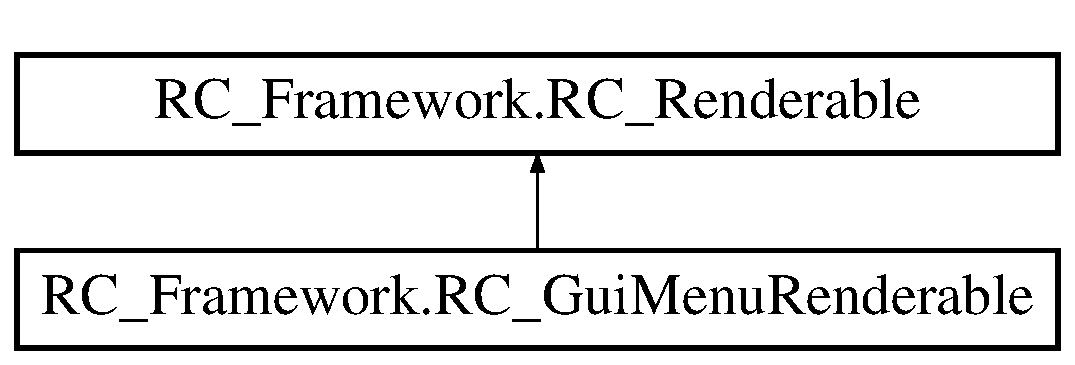
\includegraphics[height=2.000000cm]{class_r_c___framework_1_1_r_c___gui_menu_renderable}
\end{center}
\end{figure}
\subsection*{Public Member Functions}
\begin{DoxyCompactItemize}
\item 
\mbox{\hyperlink{class_r_c___framework_1_1_r_c___gui_menu_renderable_a6edd694fec762aa24a713e2b1e567ad0}{R\+C\+\_\+\+Gui\+Menu\+Renderable}} ()
\item 
void \mbox{\hyperlink{class_r_c___framework_1_1_r_c___gui_menu_renderable_a6e04c0167c6de417d89aaeb8cfd01585}{add}} (\mbox{\hyperlink{class_r_c___framework_1_1_r_c___renderable_bounded}{R\+C\+\_\+\+Renderable\+Bounded}} ren, int switch\+ValQ, float valQ)
\item 
void \mbox{\hyperlink{class_r_c___framework_1_1_r_c___gui_menu_renderable_a112c9577a1d1ac24d3eb3f308fc86191}{add\+Below}} (\mbox{\hyperlink{class_r_c___framework_1_1_r_c___renderable_bounded}{R\+C\+\_\+\+Renderable\+Bounded}} ren, int switch\+ValQ, float valQ, int gap\+In\+Pixels)
\item 
void \mbox{\hyperlink{class_r_c___framework_1_1_r_c___gui_menu_renderable_a04e2e8f730550afb71db6f700f059996}{add\+Beside}} (\mbox{\hyperlink{class_r_c___framework_1_1_r_c___renderable_bounded}{R\+C\+\_\+\+Renderable\+Bounded}} ren, int switch\+ValQ, float valQ, int gap\+In\+Pixels)
\item 
override void \mbox{\hyperlink{class_r_c___framework_1_1_r_c___gui_menu_renderable_a0c74b42e4af1cad77f708cfa174aa724}{Draw}} (Sprite\+Batch sb)
\begin{DoxyCompactList}\small\item\em Standard draw routine which assumes the renderable knows where it is \end{DoxyCompactList}\item 
override void \mbox{\hyperlink{class_r_c___framework_1_1_r_c___gui_menu_renderable_af69df1292acc0f8babaa578caebffd87}{Update}} (Game\+Time game\+Time)
\item 
override bool \mbox{\hyperlink{class_r_c___framework_1_1_r_c___gui_menu_renderable_a211b5eebda9524d97f8dfeb1f8024f32}{Mouse\+Click\+Event}} (float mouse\+\_\+x, float mouse\+\_\+y)
\item 
override bool \mbox{\hyperlink{class_r_c___framework_1_1_r_c___gui_menu_renderable_a2a1be820f5693b0badd408b5457c81bd}{Key\+Hit\+Event}} (Keys key\+Hit)
\end{DoxyCompactItemize}
\subsection*{Public Attributes}
\begin{DoxyCompactItemize}
\item 
bool \mbox{\hyperlink{class_r_c___framework_1_1_r_c___gui_menu_renderable_a400533f5ec57e37197f5b830f4f63ed9}{clicked\+This\+Frame}} = false
\begin{DoxyCompactList}\small\item\em true if a keyhit was clicked by cr (enter) or mouse to activate the button this turn \end{DoxyCompactList}\item 
bool \mbox{\hyperlink{class_r_c___framework_1_1_r_c___gui_menu_renderable_a5092508ec1a58aaef9926a1259bc13e5}{selected\+This\+Frame}} = false
\begin{DoxyCompactList}\small\item\em true if a keyhit was clicked by cr (enter) or mouse to select the button this turn \end{DoxyCompactList}\item 
Color \mbox{\hyperlink{class_r_c___framework_1_1_r_c___gui_menu_renderable_af5e943fb2d0a14e29fa96203743637b9}{highlight\+Color}} = Color.\+Black
\end{DoxyCompactItemize}
\subsection*{Additional Inherited Members}


\subsection{Detailed Description}
a sort of menu system that maintains a state called switch\+Val (int) and or val (float) It uses tag and tagint in renderable Its importent to call update before you pass in keyhit and mouseevents or the clicked\+This\+Frame will not work Its a kind of half way to a full G\+UI this suggests that renderables will ultimately replace G\+UI objects in this framework 



\subsection{Constructor \& Destructor Documentation}
\mbox{\Hypertarget{class_r_c___framework_1_1_r_c___gui_menu_renderable_a6edd694fec762aa24a713e2b1e567ad0}\label{class_r_c___framework_1_1_r_c___gui_menu_renderable_a6edd694fec762aa24a713e2b1e567ad0}} 
\index{R\+C\+\_\+\+Framework\+::\+R\+C\+\_\+\+Gui\+Menu\+Renderable@{R\+C\+\_\+\+Framework\+::\+R\+C\+\_\+\+Gui\+Menu\+Renderable}!R\+C\+\_\+\+Gui\+Menu\+Renderable@{R\+C\+\_\+\+Gui\+Menu\+Renderable}}
\index{R\+C\+\_\+\+Gui\+Menu\+Renderable@{R\+C\+\_\+\+Gui\+Menu\+Renderable}!R\+C\+\_\+\+Framework\+::\+R\+C\+\_\+\+Gui\+Menu\+Renderable@{R\+C\+\_\+\+Framework\+::\+R\+C\+\_\+\+Gui\+Menu\+Renderable}}
\subsubsection{\texorpdfstring{R\+C\+\_\+\+Gui\+Menu\+Renderable()}{RC\_GuiMenuRenderable()}}
{\footnotesize\ttfamily R\+C\+\_\+\+Framework.\+R\+C\+\_\+\+Gui\+Menu\+Renderable.\+R\+C\+\_\+\+Gui\+Menu\+Renderable (\begin{DoxyParamCaption}{ }\end{DoxyParamCaption})}



\subsection{Member Function Documentation}
\mbox{\Hypertarget{class_r_c___framework_1_1_r_c___gui_menu_renderable_a6e04c0167c6de417d89aaeb8cfd01585}\label{class_r_c___framework_1_1_r_c___gui_menu_renderable_a6e04c0167c6de417d89aaeb8cfd01585}} 
\index{R\+C\+\_\+\+Framework\+::\+R\+C\+\_\+\+Gui\+Menu\+Renderable@{R\+C\+\_\+\+Framework\+::\+R\+C\+\_\+\+Gui\+Menu\+Renderable}!add@{add}}
\index{add@{add}!R\+C\+\_\+\+Framework\+::\+R\+C\+\_\+\+Gui\+Menu\+Renderable@{R\+C\+\_\+\+Framework\+::\+R\+C\+\_\+\+Gui\+Menu\+Renderable}}
\subsubsection{\texorpdfstring{add()}{add()}}
{\footnotesize\ttfamily void R\+C\+\_\+\+Framework.\+R\+C\+\_\+\+Gui\+Menu\+Renderable.\+add (\begin{DoxyParamCaption}\item[{\mbox{\hyperlink{class_r_c___framework_1_1_r_c___renderable_bounded}{R\+C\+\_\+\+Renderable\+Bounded}}}]{ren,  }\item[{int}]{switch\+ValQ,  }\item[{float}]{valQ }\end{DoxyParamCaption})}

\mbox{\Hypertarget{class_r_c___framework_1_1_r_c___gui_menu_renderable_a112c9577a1d1ac24d3eb3f308fc86191}\label{class_r_c___framework_1_1_r_c___gui_menu_renderable_a112c9577a1d1ac24d3eb3f308fc86191}} 
\index{R\+C\+\_\+\+Framework\+::\+R\+C\+\_\+\+Gui\+Menu\+Renderable@{R\+C\+\_\+\+Framework\+::\+R\+C\+\_\+\+Gui\+Menu\+Renderable}!add\+Below@{add\+Below}}
\index{add\+Below@{add\+Below}!R\+C\+\_\+\+Framework\+::\+R\+C\+\_\+\+Gui\+Menu\+Renderable@{R\+C\+\_\+\+Framework\+::\+R\+C\+\_\+\+Gui\+Menu\+Renderable}}
\subsubsection{\texorpdfstring{add\+Below()}{addBelow()}}
{\footnotesize\ttfamily void R\+C\+\_\+\+Framework.\+R\+C\+\_\+\+Gui\+Menu\+Renderable.\+add\+Below (\begin{DoxyParamCaption}\item[{\mbox{\hyperlink{class_r_c___framework_1_1_r_c___renderable_bounded}{R\+C\+\_\+\+Renderable\+Bounded}}}]{ren,  }\item[{int}]{switch\+ValQ,  }\item[{float}]{valQ,  }\item[{int}]{gap\+In\+Pixels }\end{DoxyParamCaption})}

\mbox{\Hypertarget{class_r_c___framework_1_1_r_c___gui_menu_renderable_a04e2e8f730550afb71db6f700f059996}\label{class_r_c___framework_1_1_r_c___gui_menu_renderable_a04e2e8f730550afb71db6f700f059996}} 
\index{R\+C\+\_\+\+Framework\+::\+R\+C\+\_\+\+Gui\+Menu\+Renderable@{R\+C\+\_\+\+Framework\+::\+R\+C\+\_\+\+Gui\+Menu\+Renderable}!add\+Beside@{add\+Beside}}
\index{add\+Beside@{add\+Beside}!R\+C\+\_\+\+Framework\+::\+R\+C\+\_\+\+Gui\+Menu\+Renderable@{R\+C\+\_\+\+Framework\+::\+R\+C\+\_\+\+Gui\+Menu\+Renderable}}
\subsubsection{\texorpdfstring{add\+Beside()}{addBeside()}}
{\footnotesize\ttfamily void R\+C\+\_\+\+Framework.\+R\+C\+\_\+\+Gui\+Menu\+Renderable.\+add\+Beside (\begin{DoxyParamCaption}\item[{\mbox{\hyperlink{class_r_c___framework_1_1_r_c___renderable_bounded}{R\+C\+\_\+\+Renderable\+Bounded}}}]{ren,  }\item[{int}]{switch\+ValQ,  }\item[{float}]{valQ,  }\item[{int}]{gap\+In\+Pixels }\end{DoxyParamCaption})}

\mbox{\Hypertarget{class_r_c___framework_1_1_r_c___gui_menu_renderable_a0c74b42e4af1cad77f708cfa174aa724}\label{class_r_c___framework_1_1_r_c___gui_menu_renderable_a0c74b42e4af1cad77f708cfa174aa724}} 
\index{R\+C\+\_\+\+Framework\+::\+R\+C\+\_\+\+Gui\+Menu\+Renderable@{R\+C\+\_\+\+Framework\+::\+R\+C\+\_\+\+Gui\+Menu\+Renderable}!Draw@{Draw}}
\index{Draw@{Draw}!R\+C\+\_\+\+Framework\+::\+R\+C\+\_\+\+Gui\+Menu\+Renderable@{R\+C\+\_\+\+Framework\+::\+R\+C\+\_\+\+Gui\+Menu\+Renderable}}
\subsubsection{\texorpdfstring{Draw()}{Draw()}}
{\footnotesize\ttfamily override void R\+C\+\_\+\+Framework.\+R\+C\+\_\+\+Gui\+Menu\+Renderable.\+Draw (\begin{DoxyParamCaption}\item[{Sprite\+Batch}]{sb }\end{DoxyParamCaption})\hspace{0.3cm}{\ttfamily [virtual]}}



Standard draw routine which assumes the renderable knows where it is 


\begin{DoxyParams}{Parameters}
{\em sb} & \\
\hline
\end{DoxyParams}


Reimplemented from \mbox{\hyperlink{class_r_c___framework_1_1_r_c___renderable_acc26db34e382a25a989c4c0dd0354b23}{R\+C\+\_\+\+Framework.\+R\+C\+\_\+\+Renderable}}.

\mbox{\Hypertarget{class_r_c___framework_1_1_r_c___gui_menu_renderable_a2a1be820f5693b0badd408b5457c81bd}\label{class_r_c___framework_1_1_r_c___gui_menu_renderable_a2a1be820f5693b0badd408b5457c81bd}} 
\index{R\+C\+\_\+\+Framework\+::\+R\+C\+\_\+\+Gui\+Menu\+Renderable@{R\+C\+\_\+\+Framework\+::\+R\+C\+\_\+\+Gui\+Menu\+Renderable}!Key\+Hit\+Event@{Key\+Hit\+Event}}
\index{Key\+Hit\+Event@{Key\+Hit\+Event}!R\+C\+\_\+\+Framework\+::\+R\+C\+\_\+\+Gui\+Menu\+Renderable@{R\+C\+\_\+\+Framework\+::\+R\+C\+\_\+\+Gui\+Menu\+Renderable}}
\subsubsection{\texorpdfstring{Key\+Hit\+Event()}{KeyHitEvent()}}
{\footnotesize\ttfamily override bool R\+C\+\_\+\+Framework.\+R\+C\+\_\+\+Gui\+Menu\+Renderable.\+Key\+Hit\+Event (\begin{DoxyParamCaption}\item[{Keys}]{key\+Hit }\end{DoxyParamCaption})\hspace{0.3cm}{\ttfamily [virtual]}}



Reimplemented from \mbox{\hyperlink{class_r_c___framework_1_1_r_c___renderable_a826da9b07316c475186e4c2f00648827}{R\+C\+\_\+\+Framework.\+R\+C\+\_\+\+Renderable}}.

\mbox{\Hypertarget{class_r_c___framework_1_1_r_c___gui_menu_renderable_a211b5eebda9524d97f8dfeb1f8024f32}\label{class_r_c___framework_1_1_r_c___gui_menu_renderable_a211b5eebda9524d97f8dfeb1f8024f32}} 
\index{R\+C\+\_\+\+Framework\+::\+R\+C\+\_\+\+Gui\+Menu\+Renderable@{R\+C\+\_\+\+Framework\+::\+R\+C\+\_\+\+Gui\+Menu\+Renderable}!Mouse\+Click\+Event@{Mouse\+Click\+Event}}
\index{Mouse\+Click\+Event@{Mouse\+Click\+Event}!R\+C\+\_\+\+Framework\+::\+R\+C\+\_\+\+Gui\+Menu\+Renderable@{R\+C\+\_\+\+Framework\+::\+R\+C\+\_\+\+Gui\+Menu\+Renderable}}
\subsubsection{\texorpdfstring{Mouse\+Click\+Event()}{MouseClickEvent()}}
{\footnotesize\ttfamily override bool R\+C\+\_\+\+Framework.\+R\+C\+\_\+\+Gui\+Menu\+Renderable.\+Mouse\+Click\+Event (\begin{DoxyParamCaption}\item[{float}]{mouse\+\_\+x,  }\item[{float}]{mouse\+\_\+y }\end{DoxyParamCaption})\hspace{0.3cm}{\ttfamily [virtual]}}



Reimplemented from \mbox{\hyperlink{class_r_c___framework_1_1_r_c___renderable_af929e80b7c88bb21b01358f47ad36a64}{R\+C\+\_\+\+Framework.\+R\+C\+\_\+\+Renderable}}.

\mbox{\Hypertarget{class_r_c___framework_1_1_r_c___gui_menu_renderable_af69df1292acc0f8babaa578caebffd87}\label{class_r_c___framework_1_1_r_c___gui_menu_renderable_af69df1292acc0f8babaa578caebffd87}} 
\index{R\+C\+\_\+\+Framework\+::\+R\+C\+\_\+\+Gui\+Menu\+Renderable@{R\+C\+\_\+\+Framework\+::\+R\+C\+\_\+\+Gui\+Menu\+Renderable}!Update@{Update}}
\index{Update@{Update}!R\+C\+\_\+\+Framework\+::\+R\+C\+\_\+\+Gui\+Menu\+Renderable@{R\+C\+\_\+\+Framework\+::\+R\+C\+\_\+\+Gui\+Menu\+Renderable}}
\subsubsection{\texorpdfstring{Update()}{Update()}}
{\footnotesize\ttfamily override void R\+C\+\_\+\+Framework.\+R\+C\+\_\+\+Gui\+Menu\+Renderable.\+Update (\begin{DoxyParamCaption}\item[{Game\+Time}]{game\+Time }\end{DoxyParamCaption})\hspace{0.3cm}{\ttfamily [virtual]}}



Reimplemented from \mbox{\hyperlink{class_r_c___framework_1_1_r_c___renderable_a5745bedc7ba0587aa1e1d8563c357228}{R\+C\+\_\+\+Framework.\+R\+C\+\_\+\+Renderable}}.



\subsection{Member Data Documentation}
\mbox{\Hypertarget{class_r_c___framework_1_1_r_c___gui_menu_renderable_a400533f5ec57e37197f5b830f4f63ed9}\label{class_r_c___framework_1_1_r_c___gui_menu_renderable_a400533f5ec57e37197f5b830f4f63ed9}} 
\index{R\+C\+\_\+\+Framework\+::\+R\+C\+\_\+\+Gui\+Menu\+Renderable@{R\+C\+\_\+\+Framework\+::\+R\+C\+\_\+\+Gui\+Menu\+Renderable}!clicked\+This\+Frame@{clicked\+This\+Frame}}
\index{clicked\+This\+Frame@{clicked\+This\+Frame}!R\+C\+\_\+\+Framework\+::\+R\+C\+\_\+\+Gui\+Menu\+Renderable@{R\+C\+\_\+\+Framework\+::\+R\+C\+\_\+\+Gui\+Menu\+Renderable}}
\subsubsection{\texorpdfstring{clicked\+This\+Frame}{clickedThisFrame}}
{\footnotesize\ttfamily bool R\+C\+\_\+\+Framework.\+R\+C\+\_\+\+Gui\+Menu\+Renderable.\+clicked\+This\+Frame = false}



true if a keyhit was clicked by cr (enter) or mouse to activate the button this turn 

\mbox{\Hypertarget{class_r_c___framework_1_1_r_c___gui_menu_renderable_af5e943fb2d0a14e29fa96203743637b9}\label{class_r_c___framework_1_1_r_c___gui_menu_renderable_af5e943fb2d0a14e29fa96203743637b9}} 
\index{R\+C\+\_\+\+Framework\+::\+R\+C\+\_\+\+Gui\+Menu\+Renderable@{R\+C\+\_\+\+Framework\+::\+R\+C\+\_\+\+Gui\+Menu\+Renderable}!highlight\+Color@{highlight\+Color}}
\index{highlight\+Color@{highlight\+Color}!R\+C\+\_\+\+Framework\+::\+R\+C\+\_\+\+Gui\+Menu\+Renderable@{R\+C\+\_\+\+Framework\+::\+R\+C\+\_\+\+Gui\+Menu\+Renderable}}
\subsubsection{\texorpdfstring{highlight\+Color}{highlightColor}}
{\footnotesize\ttfamily Color R\+C\+\_\+\+Framework.\+R\+C\+\_\+\+Gui\+Menu\+Renderable.\+highlight\+Color = Color.\+Black}

\mbox{\Hypertarget{class_r_c___framework_1_1_r_c___gui_menu_renderable_a5092508ec1a58aaef9926a1259bc13e5}\label{class_r_c___framework_1_1_r_c___gui_menu_renderable_a5092508ec1a58aaef9926a1259bc13e5}} 
\index{R\+C\+\_\+\+Framework\+::\+R\+C\+\_\+\+Gui\+Menu\+Renderable@{R\+C\+\_\+\+Framework\+::\+R\+C\+\_\+\+Gui\+Menu\+Renderable}!selected\+This\+Frame@{selected\+This\+Frame}}
\index{selected\+This\+Frame@{selected\+This\+Frame}!R\+C\+\_\+\+Framework\+::\+R\+C\+\_\+\+Gui\+Menu\+Renderable@{R\+C\+\_\+\+Framework\+::\+R\+C\+\_\+\+Gui\+Menu\+Renderable}}
\subsubsection{\texorpdfstring{selected\+This\+Frame}{selectedThisFrame}}
{\footnotesize\ttfamily bool R\+C\+\_\+\+Framework.\+R\+C\+\_\+\+Gui\+Menu\+Renderable.\+selected\+This\+Frame = false}



true if a keyhit was clicked by cr (enter) or mouse to select the button this turn 



The documentation for this class was generated from the following file\+:\begin{DoxyCompactItemize}
\item 
F\+:/\+B/\+R\+C\+\_\+\+Framework2018/\+Source/\mbox{\hyperlink{_r_c___g_u_i_menu_renderable_8cs}{R\+C\+\_\+\+G\+U\+I\+Menu\+Renderable.\+cs}}\end{DoxyCompactItemize}

\hypertarget{class_r_c___framework_1_1_r_c__pos_in_circle}{}\section{R\+C\+\_\+\+Framework.\+R\+C\+\_\+pos\+In\+Circle Class Reference}
\label{class_r_c___framework_1_1_r_c__pos_in_circle}\index{R\+C\+\_\+\+Framework.\+R\+C\+\_\+pos\+In\+Circle@{R\+C\+\_\+\+Framework.\+R\+C\+\_\+pos\+In\+Circle}}


Creates positions inside the rectangle inclusive of top and left exclusive of right and bottom  


Inheritance diagram for R\+C\+\_\+\+Framework.\+R\+C\+\_\+pos\+In\+Circle\+:\begin{figure}[H]
\begin{center}
\leavevmode
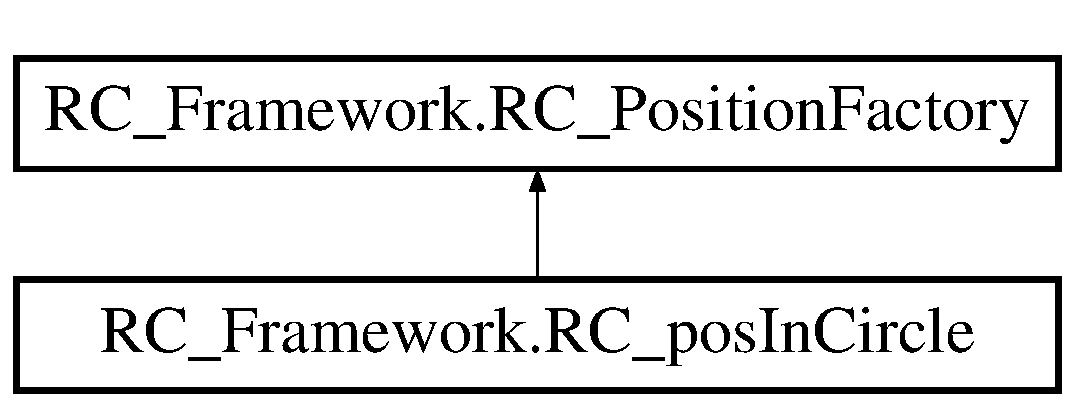
\includegraphics[height=2.000000cm]{class_r_c___framework_1_1_r_c__pos_in_circle}
\end{center}
\end{figure}
\subsection*{Public Member Functions}
\begin{DoxyCompactItemize}
\item 
\mbox{\hyperlink{class_r_c___framework_1_1_r_c__pos_in_circle_a6f5bee60c5ab75935b6ce528473f8b9f}{R\+C\+\_\+pos\+In\+Circle}} (Vector2 posZ, float radius\+MinZ, float radius\+MaxZ, Random rndZ)
\item 
override Vector2 \mbox{\hyperlink{class_r_c___framework_1_1_r_c__pos_in_circle_a4cec38bb6d1617a7ad918d59c5125df9}{get\+Next\+Pos}} ()
\item 
override void \mbox{\hyperlink{class_r_c___framework_1_1_r_c__pos_in_circle_ad59a9527d30ddfa0b15c4210907d3051}{draw}} (Sprite\+Batch sb, Color col)
\end{DoxyCompactItemize}


\subsection{Detailed Description}
Creates positions inside the rectangle inclusive of top and left exclusive of right and bottom 



\subsection{Constructor \& Destructor Documentation}
\mbox{\Hypertarget{class_r_c___framework_1_1_r_c__pos_in_circle_a6f5bee60c5ab75935b6ce528473f8b9f}\label{class_r_c___framework_1_1_r_c__pos_in_circle_a6f5bee60c5ab75935b6ce528473f8b9f}} 
\index{R\+C\+\_\+\+Framework\+::\+R\+C\+\_\+pos\+In\+Circle@{R\+C\+\_\+\+Framework\+::\+R\+C\+\_\+pos\+In\+Circle}!R\+C\+\_\+pos\+In\+Circle@{R\+C\+\_\+pos\+In\+Circle}}
\index{R\+C\+\_\+pos\+In\+Circle@{R\+C\+\_\+pos\+In\+Circle}!R\+C\+\_\+\+Framework\+::\+R\+C\+\_\+pos\+In\+Circle@{R\+C\+\_\+\+Framework\+::\+R\+C\+\_\+pos\+In\+Circle}}
\subsubsection{\texorpdfstring{R\+C\+\_\+pos\+In\+Circle()}{RC\_posInCircle()}}
{\footnotesize\ttfamily R\+C\+\_\+\+Framework.\+R\+C\+\_\+pos\+In\+Circle.\+R\+C\+\_\+pos\+In\+Circle (\begin{DoxyParamCaption}\item[{Vector2}]{posZ,  }\item[{float}]{radius\+MinZ,  }\item[{float}]{radius\+MaxZ,  }\item[{Random}]{rndZ }\end{DoxyParamCaption})}



\subsection{Member Function Documentation}
\mbox{\Hypertarget{class_r_c___framework_1_1_r_c__pos_in_circle_ad59a9527d30ddfa0b15c4210907d3051}\label{class_r_c___framework_1_1_r_c__pos_in_circle_ad59a9527d30ddfa0b15c4210907d3051}} 
\index{R\+C\+\_\+\+Framework\+::\+R\+C\+\_\+pos\+In\+Circle@{R\+C\+\_\+\+Framework\+::\+R\+C\+\_\+pos\+In\+Circle}!draw@{draw}}
\index{draw@{draw}!R\+C\+\_\+\+Framework\+::\+R\+C\+\_\+pos\+In\+Circle@{R\+C\+\_\+\+Framework\+::\+R\+C\+\_\+pos\+In\+Circle}}
\subsubsection{\texorpdfstring{draw()}{draw()}}
{\footnotesize\ttfamily override void R\+C\+\_\+\+Framework.\+R\+C\+\_\+pos\+In\+Circle.\+draw (\begin{DoxyParamCaption}\item[{Sprite\+Batch}]{sb,  }\item[{Color}]{col }\end{DoxyParamCaption})\hspace{0.3cm}{\ttfamily [virtual]}}



Reimplemented from \mbox{\hyperlink{class_r_c___framework_1_1_r_c___position_factory_a39eaa0f4f1dfd07225b4880d494d81fa}{R\+C\+\_\+\+Framework.\+R\+C\+\_\+\+Position\+Factory}}.

\mbox{\Hypertarget{class_r_c___framework_1_1_r_c__pos_in_circle_a4cec38bb6d1617a7ad918d59c5125df9}\label{class_r_c___framework_1_1_r_c__pos_in_circle_a4cec38bb6d1617a7ad918d59c5125df9}} 
\index{R\+C\+\_\+\+Framework\+::\+R\+C\+\_\+pos\+In\+Circle@{R\+C\+\_\+\+Framework\+::\+R\+C\+\_\+pos\+In\+Circle}!get\+Next\+Pos@{get\+Next\+Pos}}
\index{get\+Next\+Pos@{get\+Next\+Pos}!R\+C\+\_\+\+Framework\+::\+R\+C\+\_\+pos\+In\+Circle@{R\+C\+\_\+\+Framework\+::\+R\+C\+\_\+pos\+In\+Circle}}
\subsubsection{\texorpdfstring{get\+Next\+Pos()}{getNextPos()}}
{\footnotesize\ttfamily override Vector2 R\+C\+\_\+\+Framework.\+R\+C\+\_\+pos\+In\+Circle.\+get\+Next\+Pos (\begin{DoxyParamCaption}{ }\end{DoxyParamCaption})\hspace{0.3cm}{\ttfamily [virtual]}}



Implements \mbox{\hyperlink{class_r_c___framework_1_1_r_c___position_factory_aab6cd4cb6a10c8dfa126c4930c6a9fbf}{R\+C\+\_\+\+Framework.\+R\+C\+\_\+\+Position\+Factory}}.



The documentation for this class was generated from the following file\+:\begin{DoxyCompactItemize}
\item 
F\+:/\+B/\+R\+C\+\_\+\+Framework2018/\+Source/\mbox{\hyperlink{_r_c___position_factory_8cs}{R\+C\+\_\+\+Position\+Factory.\+cs}}\end{DoxyCompactItemize}

\hypertarget{class_r_c___framework_1_1_r_c__pos_inrectangle}{}\section{R\+C\+\_\+\+Framework.\+R\+C\+\_\+pos\+Inrectangle Class Reference}
\label{class_r_c___framework_1_1_r_c__pos_inrectangle}\index{R\+C\+\_\+\+Framework.\+R\+C\+\_\+pos\+Inrectangle@{R\+C\+\_\+\+Framework.\+R\+C\+\_\+pos\+Inrectangle}}


Creates positions inside the rectangle inclusive of top and left exclusive of right and bottom N\+O\+TE Also usefull for vertical or horizontal line with width or height 1  


Inheritance diagram for R\+C\+\_\+\+Framework.\+R\+C\+\_\+pos\+Inrectangle\+:\begin{figure}[H]
\begin{center}
\leavevmode
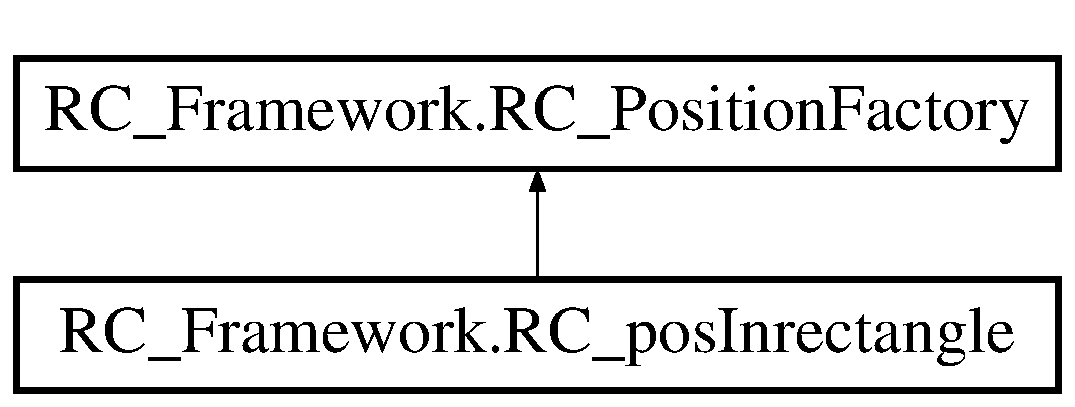
\includegraphics[height=2.000000cm]{class_r_c___framework_1_1_r_c__pos_inrectangle}
\end{center}
\end{figure}
\subsection*{Public Member Functions}
\begin{DoxyCompactItemize}
\item 
\mbox{\hyperlink{class_r_c___framework_1_1_r_c__pos_inrectangle_a45d6ba0898613aeb2b8d0762f33ad87b}{R\+C\+\_\+pos\+Inrectangle}} (Rectangle r, Random rndZ)
\item 
override Vector2 \mbox{\hyperlink{class_r_c___framework_1_1_r_c__pos_inrectangle_aafd0da0c3d4742c9aade81342125af81}{get\+Next\+Pos}} ()
\item 
override void \mbox{\hyperlink{class_r_c___framework_1_1_r_c__pos_inrectangle_ab5a236d69d4dc284f825e4e4d28908ec}{draw}} (Sprite\+Batch sb, Color col)
\end{DoxyCompactItemize}


\subsection{Detailed Description}
Creates positions inside the rectangle inclusive of top and left exclusive of right and bottom N\+O\+TE Also usefull for vertical or horizontal line with width or height 1 



\subsection{Constructor \& Destructor Documentation}
\mbox{\Hypertarget{class_r_c___framework_1_1_r_c__pos_inrectangle_a45d6ba0898613aeb2b8d0762f33ad87b}\label{class_r_c___framework_1_1_r_c__pos_inrectangle_a45d6ba0898613aeb2b8d0762f33ad87b}} 
\index{R\+C\+\_\+\+Framework\+::\+R\+C\+\_\+pos\+Inrectangle@{R\+C\+\_\+\+Framework\+::\+R\+C\+\_\+pos\+Inrectangle}!R\+C\+\_\+pos\+Inrectangle@{R\+C\+\_\+pos\+Inrectangle}}
\index{R\+C\+\_\+pos\+Inrectangle@{R\+C\+\_\+pos\+Inrectangle}!R\+C\+\_\+\+Framework\+::\+R\+C\+\_\+pos\+Inrectangle@{R\+C\+\_\+\+Framework\+::\+R\+C\+\_\+pos\+Inrectangle}}
\subsubsection{\texorpdfstring{R\+C\+\_\+pos\+Inrectangle()}{RC\_posInrectangle()}}
{\footnotesize\ttfamily R\+C\+\_\+\+Framework.\+R\+C\+\_\+pos\+Inrectangle.\+R\+C\+\_\+pos\+Inrectangle (\begin{DoxyParamCaption}\item[{Rectangle}]{r,  }\item[{Random}]{rndZ }\end{DoxyParamCaption})}



\subsection{Member Function Documentation}
\mbox{\Hypertarget{class_r_c___framework_1_1_r_c__pos_inrectangle_ab5a236d69d4dc284f825e4e4d28908ec}\label{class_r_c___framework_1_1_r_c__pos_inrectangle_ab5a236d69d4dc284f825e4e4d28908ec}} 
\index{R\+C\+\_\+\+Framework\+::\+R\+C\+\_\+pos\+Inrectangle@{R\+C\+\_\+\+Framework\+::\+R\+C\+\_\+pos\+Inrectangle}!draw@{draw}}
\index{draw@{draw}!R\+C\+\_\+\+Framework\+::\+R\+C\+\_\+pos\+Inrectangle@{R\+C\+\_\+\+Framework\+::\+R\+C\+\_\+pos\+Inrectangle}}
\subsubsection{\texorpdfstring{draw()}{draw()}}
{\footnotesize\ttfamily override void R\+C\+\_\+\+Framework.\+R\+C\+\_\+pos\+Inrectangle.\+draw (\begin{DoxyParamCaption}\item[{Sprite\+Batch}]{sb,  }\item[{Color}]{col }\end{DoxyParamCaption})\hspace{0.3cm}{\ttfamily [virtual]}}



Reimplemented from \mbox{\hyperlink{class_r_c___framework_1_1_r_c___position_factory_a39eaa0f4f1dfd07225b4880d494d81fa}{R\+C\+\_\+\+Framework.\+R\+C\+\_\+\+Position\+Factory}}.

\mbox{\Hypertarget{class_r_c___framework_1_1_r_c__pos_inrectangle_aafd0da0c3d4742c9aade81342125af81}\label{class_r_c___framework_1_1_r_c__pos_inrectangle_aafd0da0c3d4742c9aade81342125af81}} 
\index{R\+C\+\_\+\+Framework\+::\+R\+C\+\_\+pos\+Inrectangle@{R\+C\+\_\+\+Framework\+::\+R\+C\+\_\+pos\+Inrectangle}!get\+Next\+Pos@{get\+Next\+Pos}}
\index{get\+Next\+Pos@{get\+Next\+Pos}!R\+C\+\_\+\+Framework\+::\+R\+C\+\_\+pos\+Inrectangle@{R\+C\+\_\+\+Framework\+::\+R\+C\+\_\+pos\+Inrectangle}}
\subsubsection{\texorpdfstring{get\+Next\+Pos()}{getNextPos()}}
{\footnotesize\ttfamily override Vector2 R\+C\+\_\+\+Framework.\+R\+C\+\_\+pos\+Inrectangle.\+get\+Next\+Pos (\begin{DoxyParamCaption}{ }\end{DoxyParamCaption})\hspace{0.3cm}{\ttfamily [virtual]}}



Implements \mbox{\hyperlink{class_r_c___framework_1_1_r_c___position_factory_aab6cd4cb6a10c8dfa126c4930c6a9fbf}{R\+C\+\_\+\+Framework.\+R\+C\+\_\+\+Position\+Factory}}.



The documentation for this class was generated from the following file\+:\begin{DoxyCompactItemize}
\item 
F\+:/\+B/\+R\+C\+\_\+\+Framework2018/\+Source/\mbox{\hyperlink{_r_c___position_factory_8cs}{R\+C\+\_\+\+Position\+Factory.\+cs}}\end{DoxyCompactItemize}

\hypertarget{class_r_c___framework_1_1_r_c___position_factory}{}\section{R\+C\+\_\+\+Framework.\+R\+C\+\_\+\+Position\+Factory Class Reference}
\label{class_r_c___framework_1_1_r_c___position_factory}\index{R\+C\+\_\+\+Framework.\+R\+C\+\_\+\+Position\+Factory@{R\+C\+\_\+\+Framework.\+R\+C\+\_\+\+Position\+Factory}}


parent class for all position factories  


Inheritance diagram for R\+C\+\_\+\+Framework.\+R\+C\+\_\+\+Position\+Factory\+:\begin{figure}[H]
\begin{center}
\leavevmode
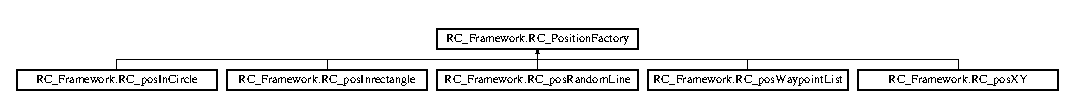
\includegraphics[height=0.991150cm]{class_r_c___framework_1_1_r_c___position_factory}
\end{center}
\end{figure}
\subsection*{Public Member Functions}
\begin{DoxyCompactItemize}
\item 
abstract Vector2 \mbox{\hyperlink{class_r_c___framework_1_1_r_c___position_factory_aab6cd4cb6a10c8dfa126c4930c6a9fbf}{get\+Next\+Pos}} ()
\item 
virtual void \mbox{\hyperlink{class_r_c___framework_1_1_r_c___position_factory_af966db836e692a5a485531d227caa944}{init}} ()
\item 
virtual void \mbox{\hyperlink{class_r_c___framework_1_1_r_c___position_factory_a582a8b01a360280d67b199b1190d96f7}{reset}} ()
\item 
virtual void \mbox{\hyperlink{class_r_c___framework_1_1_r_c___position_factory_a39eaa0f4f1dfd07225b4880d494d81fa}{draw}} (Sprite\+Batch sb, Color col)
\end{DoxyCompactItemize}


\subsection{Detailed Description}
parent class for all position factories 



\subsection{Member Function Documentation}
\mbox{\Hypertarget{class_r_c___framework_1_1_r_c___position_factory_a39eaa0f4f1dfd07225b4880d494d81fa}\label{class_r_c___framework_1_1_r_c___position_factory_a39eaa0f4f1dfd07225b4880d494d81fa}} 
\index{R\+C\+\_\+\+Framework\+::\+R\+C\+\_\+\+Position\+Factory@{R\+C\+\_\+\+Framework\+::\+R\+C\+\_\+\+Position\+Factory}!draw@{draw}}
\index{draw@{draw}!R\+C\+\_\+\+Framework\+::\+R\+C\+\_\+\+Position\+Factory@{R\+C\+\_\+\+Framework\+::\+R\+C\+\_\+\+Position\+Factory}}
\subsubsection{\texorpdfstring{draw()}{draw()}}
{\footnotesize\ttfamily virtual void R\+C\+\_\+\+Framework.\+R\+C\+\_\+\+Position\+Factory.\+draw (\begin{DoxyParamCaption}\item[{Sprite\+Batch}]{sb,  }\item[{Color}]{col }\end{DoxyParamCaption})\hspace{0.3cm}{\ttfamily [virtual]}}



Reimplemented in \mbox{\hyperlink{class_r_c___framework_1_1_r_c__pos_waypoint_list_ae0bea3900f15e35e022f9b1d5c409067}{R\+C\+\_\+\+Framework.\+R\+C\+\_\+pos\+Waypoint\+List}}, \mbox{\hyperlink{class_r_c___framework_1_1_r_c__pos_random_line_aa0c6137f7d33d80534376f2c4f9612e6}{R\+C\+\_\+\+Framework.\+R\+C\+\_\+pos\+Random\+Line}}, \mbox{\hyperlink{class_r_c___framework_1_1_r_c__pos_x_y_aaf344770b6a98b98937f4d43ffd536ef}{R\+C\+\_\+\+Framework.\+R\+C\+\_\+pos\+XY}}, \mbox{\hyperlink{class_r_c___framework_1_1_r_c__pos_in_circle_ad59a9527d30ddfa0b15c4210907d3051}{R\+C\+\_\+\+Framework.\+R\+C\+\_\+pos\+In\+Circle}}, and \mbox{\hyperlink{class_r_c___framework_1_1_r_c__pos_inrectangle_ab5a236d69d4dc284f825e4e4d28908ec}{R\+C\+\_\+\+Framework.\+R\+C\+\_\+pos\+Inrectangle}}.

\mbox{\Hypertarget{class_r_c___framework_1_1_r_c___position_factory_aab6cd4cb6a10c8dfa126c4930c6a9fbf}\label{class_r_c___framework_1_1_r_c___position_factory_aab6cd4cb6a10c8dfa126c4930c6a9fbf}} 
\index{R\+C\+\_\+\+Framework\+::\+R\+C\+\_\+\+Position\+Factory@{R\+C\+\_\+\+Framework\+::\+R\+C\+\_\+\+Position\+Factory}!get\+Next\+Pos@{get\+Next\+Pos}}
\index{get\+Next\+Pos@{get\+Next\+Pos}!R\+C\+\_\+\+Framework\+::\+R\+C\+\_\+\+Position\+Factory@{R\+C\+\_\+\+Framework\+::\+R\+C\+\_\+\+Position\+Factory}}
\subsubsection{\texorpdfstring{get\+Next\+Pos()}{getNextPos()}}
{\footnotesize\ttfamily abstract Vector2 R\+C\+\_\+\+Framework.\+R\+C\+\_\+\+Position\+Factory.\+get\+Next\+Pos (\begin{DoxyParamCaption}{ }\end{DoxyParamCaption})\hspace{0.3cm}{\ttfamily [pure virtual]}}



Implemented in \mbox{\hyperlink{class_r_c___framework_1_1_r_c__pos_waypoint_list_a2f91d419c6513795cae3464fda807450}{R\+C\+\_\+\+Framework.\+R\+C\+\_\+pos\+Waypoint\+List}}, \mbox{\hyperlink{class_r_c___framework_1_1_r_c__pos_random_line_ad5a37e0d9cc9baea5d0a3f8b6b80bd9e}{R\+C\+\_\+\+Framework.\+R\+C\+\_\+pos\+Random\+Line}}, \mbox{\hyperlink{class_r_c___framework_1_1_r_c__pos_x_y_a773d0a5b2b6bfc49510dbecdfbf1f9cc}{R\+C\+\_\+\+Framework.\+R\+C\+\_\+pos\+XY}}, \mbox{\hyperlink{class_r_c___framework_1_1_r_c__pos_in_circle_a4cec38bb6d1617a7ad918d59c5125df9}{R\+C\+\_\+\+Framework.\+R\+C\+\_\+pos\+In\+Circle}}, and \mbox{\hyperlink{class_r_c___framework_1_1_r_c__pos_inrectangle_aafd0da0c3d4742c9aade81342125af81}{R\+C\+\_\+\+Framework.\+R\+C\+\_\+pos\+Inrectangle}}.

\mbox{\Hypertarget{class_r_c___framework_1_1_r_c___position_factory_af966db836e692a5a485531d227caa944}\label{class_r_c___framework_1_1_r_c___position_factory_af966db836e692a5a485531d227caa944}} 
\index{R\+C\+\_\+\+Framework\+::\+R\+C\+\_\+\+Position\+Factory@{R\+C\+\_\+\+Framework\+::\+R\+C\+\_\+\+Position\+Factory}!init@{init}}
\index{init@{init}!R\+C\+\_\+\+Framework\+::\+R\+C\+\_\+\+Position\+Factory@{R\+C\+\_\+\+Framework\+::\+R\+C\+\_\+\+Position\+Factory}}
\subsubsection{\texorpdfstring{init()}{init()}}
{\footnotesize\ttfamily virtual void R\+C\+\_\+\+Framework.\+R\+C\+\_\+\+Position\+Factory.\+init (\begin{DoxyParamCaption}{ }\end{DoxyParamCaption})\hspace{0.3cm}{\ttfamily [virtual]}}



Reimplemented in \mbox{\hyperlink{class_r_c___framework_1_1_r_c__pos_waypoint_list_a9bd29086f89fd9b6ad534dbf1d2785ab}{R\+C\+\_\+\+Framework.\+R\+C\+\_\+pos\+Waypoint\+List}}.

\mbox{\Hypertarget{class_r_c___framework_1_1_r_c___position_factory_a582a8b01a360280d67b199b1190d96f7}\label{class_r_c___framework_1_1_r_c___position_factory_a582a8b01a360280d67b199b1190d96f7}} 
\index{R\+C\+\_\+\+Framework\+::\+R\+C\+\_\+\+Position\+Factory@{R\+C\+\_\+\+Framework\+::\+R\+C\+\_\+\+Position\+Factory}!reset@{reset}}
\index{reset@{reset}!R\+C\+\_\+\+Framework\+::\+R\+C\+\_\+\+Position\+Factory@{R\+C\+\_\+\+Framework\+::\+R\+C\+\_\+\+Position\+Factory}}
\subsubsection{\texorpdfstring{reset()}{reset()}}
{\footnotesize\ttfamily virtual void R\+C\+\_\+\+Framework.\+R\+C\+\_\+\+Position\+Factory.\+reset (\begin{DoxyParamCaption}{ }\end{DoxyParamCaption})\hspace{0.3cm}{\ttfamily [virtual]}}



Reimplemented in \mbox{\hyperlink{class_r_c___framework_1_1_r_c__pos_waypoint_list_acb5b5300a57cd6fc7c24db08bb27cdbf}{R\+C\+\_\+\+Framework.\+R\+C\+\_\+pos\+Waypoint\+List}}.



The documentation for this class was generated from the following file\+:\begin{DoxyCompactItemize}
\item 
F\+:/\+B/\+R\+C\+\_\+\+Framework2018/\+Source/\mbox{\hyperlink{_r_c___position_factory_8cs}{R\+C\+\_\+\+Position\+Factory.\+cs}}\end{DoxyCompactItemize}

\hypertarget{class_r_c___framework_1_1_r_c__pos_random_line}{}\section{R\+C\+\_\+\+Framework.\+R\+C\+\_\+pos\+Random\+Line Class Reference}
\label{class_r_c___framework_1_1_r_c__pos_random_line}\index{R\+C\+\_\+\+Framework.\+R\+C\+\_\+pos\+Random\+Line@{R\+C\+\_\+\+Framework.\+R\+C\+\_\+pos\+Random\+Line}}


Creates positions which are just random on an arbitary line inclusive (includes both end points)  


Inheritance diagram for R\+C\+\_\+\+Framework.\+R\+C\+\_\+pos\+Random\+Line\+:\begin{figure}[H]
\begin{center}
\leavevmode
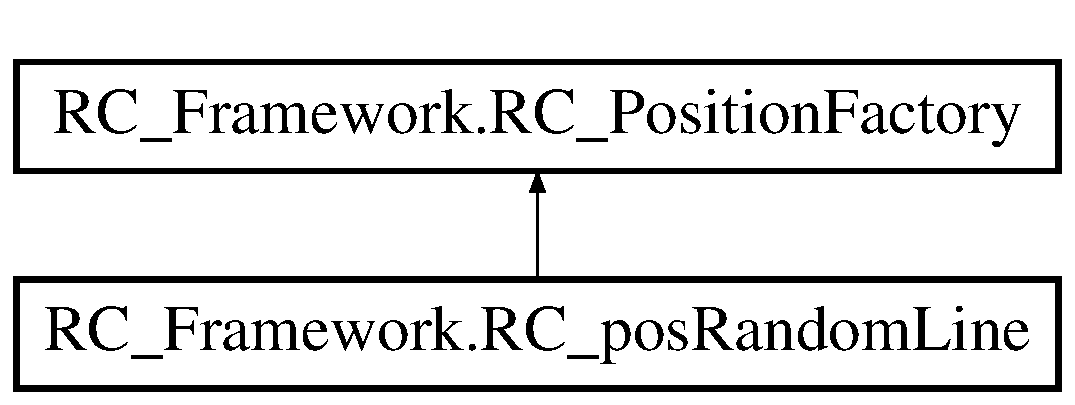
\includegraphics[height=2.000000cm]{class_r_c___framework_1_1_r_c__pos_random_line}
\end{center}
\end{figure}
\subsection*{Public Member Functions}
\begin{DoxyCompactItemize}
\item 
\mbox{\hyperlink{class_r_c___framework_1_1_r_c__pos_random_line_af5be3614b3a992075132dbc476d50abd}{R\+C\+\_\+pos\+Random\+Line}} (Vector2 fromQ, Vector2 toQ, Random rndZ)
\item 
override Vector2 \mbox{\hyperlink{class_r_c___framework_1_1_r_c__pos_random_line_ad5a37e0d9cc9baea5d0a3f8b6b80bd9e}{get\+Next\+Pos}} ()
\item 
override void \mbox{\hyperlink{class_r_c___framework_1_1_r_c__pos_random_line_aa0c6137f7d33d80534376f2c4f9612e6}{draw}} (Sprite\+Batch sb, Color col)
\end{DoxyCompactItemize}
\subsection*{Public Attributes}
\begin{DoxyCompactItemize}
\item 
Vector2 \mbox{\hyperlink{class_r_c___framework_1_1_r_c__pos_random_line_abd0ae43a0ce2bff5d147fb70159d336d}{pos\+From}} = new Vector2(100, 100)
\item 
Vector2 \mbox{\hyperlink{class_r_c___framework_1_1_r_c__pos_random_line_a94be18c12a06b0b082996478b08f36a1}{pos\+To}} = new Vector2(200, 200)
\end{DoxyCompactItemize}


\subsection{Detailed Description}
Creates positions which are just random on an arbitary line inclusive (includes both end points) 



\subsection{Constructor \& Destructor Documentation}
\mbox{\Hypertarget{class_r_c___framework_1_1_r_c__pos_random_line_af5be3614b3a992075132dbc476d50abd}\label{class_r_c___framework_1_1_r_c__pos_random_line_af5be3614b3a992075132dbc476d50abd}} 
\index{R\+C\+\_\+\+Framework\+::\+R\+C\+\_\+pos\+Random\+Line@{R\+C\+\_\+\+Framework\+::\+R\+C\+\_\+pos\+Random\+Line}!R\+C\+\_\+pos\+Random\+Line@{R\+C\+\_\+pos\+Random\+Line}}
\index{R\+C\+\_\+pos\+Random\+Line@{R\+C\+\_\+pos\+Random\+Line}!R\+C\+\_\+\+Framework\+::\+R\+C\+\_\+pos\+Random\+Line@{R\+C\+\_\+\+Framework\+::\+R\+C\+\_\+pos\+Random\+Line}}
\subsubsection{\texorpdfstring{R\+C\+\_\+pos\+Random\+Line()}{RC\_posRandomLine()}}
{\footnotesize\ttfamily R\+C\+\_\+\+Framework.\+R\+C\+\_\+pos\+Random\+Line.\+R\+C\+\_\+pos\+Random\+Line (\begin{DoxyParamCaption}\item[{Vector2}]{fromQ,  }\item[{Vector2}]{toQ,  }\item[{Random}]{rndZ }\end{DoxyParamCaption})}



\subsection{Member Function Documentation}
\mbox{\Hypertarget{class_r_c___framework_1_1_r_c__pos_random_line_aa0c6137f7d33d80534376f2c4f9612e6}\label{class_r_c___framework_1_1_r_c__pos_random_line_aa0c6137f7d33d80534376f2c4f9612e6}} 
\index{R\+C\+\_\+\+Framework\+::\+R\+C\+\_\+pos\+Random\+Line@{R\+C\+\_\+\+Framework\+::\+R\+C\+\_\+pos\+Random\+Line}!draw@{draw}}
\index{draw@{draw}!R\+C\+\_\+\+Framework\+::\+R\+C\+\_\+pos\+Random\+Line@{R\+C\+\_\+\+Framework\+::\+R\+C\+\_\+pos\+Random\+Line}}
\subsubsection{\texorpdfstring{draw()}{draw()}}
{\footnotesize\ttfamily override void R\+C\+\_\+\+Framework.\+R\+C\+\_\+pos\+Random\+Line.\+draw (\begin{DoxyParamCaption}\item[{Sprite\+Batch}]{sb,  }\item[{Color}]{col }\end{DoxyParamCaption})\hspace{0.3cm}{\ttfamily [virtual]}}



Reimplemented from \mbox{\hyperlink{class_r_c___framework_1_1_r_c___position_factory_a39eaa0f4f1dfd07225b4880d494d81fa}{R\+C\+\_\+\+Framework.\+R\+C\+\_\+\+Position\+Factory}}.

\mbox{\Hypertarget{class_r_c___framework_1_1_r_c__pos_random_line_ad5a37e0d9cc9baea5d0a3f8b6b80bd9e}\label{class_r_c___framework_1_1_r_c__pos_random_line_ad5a37e0d9cc9baea5d0a3f8b6b80bd9e}} 
\index{R\+C\+\_\+\+Framework\+::\+R\+C\+\_\+pos\+Random\+Line@{R\+C\+\_\+\+Framework\+::\+R\+C\+\_\+pos\+Random\+Line}!get\+Next\+Pos@{get\+Next\+Pos}}
\index{get\+Next\+Pos@{get\+Next\+Pos}!R\+C\+\_\+\+Framework\+::\+R\+C\+\_\+pos\+Random\+Line@{R\+C\+\_\+\+Framework\+::\+R\+C\+\_\+pos\+Random\+Line}}
\subsubsection{\texorpdfstring{get\+Next\+Pos()}{getNextPos()}}
{\footnotesize\ttfamily override Vector2 R\+C\+\_\+\+Framework.\+R\+C\+\_\+pos\+Random\+Line.\+get\+Next\+Pos (\begin{DoxyParamCaption}{ }\end{DoxyParamCaption})\hspace{0.3cm}{\ttfamily [virtual]}}



Implements \mbox{\hyperlink{class_r_c___framework_1_1_r_c___position_factory_aab6cd4cb6a10c8dfa126c4930c6a9fbf}{R\+C\+\_\+\+Framework.\+R\+C\+\_\+\+Position\+Factory}}.



\subsection{Member Data Documentation}
\mbox{\Hypertarget{class_r_c___framework_1_1_r_c__pos_random_line_abd0ae43a0ce2bff5d147fb70159d336d}\label{class_r_c___framework_1_1_r_c__pos_random_line_abd0ae43a0ce2bff5d147fb70159d336d}} 
\index{R\+C\+\_\+\+Framework\+::\+R\+C\+\_\+pos\+Random\+Line@{R\+C\+\_\+\+Framework\+::\+R\+C\+\_\+pos\+Random\+Line}!pos\+From@{pos\+From}}
\index{pos\+From@{pos\+From}!R\+C\+\_\+\+Framework\+::\+R\+C\+\_\+pos\+Random\+Line@{R\+C\+\_\+\+Framework\+::\+R\+C\+\_\+pos\+Random\+Line}}
\subsubsection{\texorpdfstring{pos\+From}{posFrom}}
{\footnotesize\ttfamily Vector2 R\+C\+\_\+\+Framework.\+R\+C\+\_\+pos\+Random\+Line.\+pos\+From = new Vector2(100, 100)}

\mbox{\Hypertarget{class_r_c___framework_1_1_r_c__pos_random_line_a94be18c12a06b0b082996478b08f36a1}\label{class_r_c___framework_1_1_r_c__pos_random_line_a94be18c12a06b0b082996478b08f36a1}} 
\index{R\+C\+\_\+\+Framework\+::\+R\+C\+\_\+pos\+Random\+Line@{R\+C\+\_\+\+Framework\+::\+R\+C\+\_\+pos\+Random\+Line}!pos\+To@{pos\+To}}
\index{pos\+To@{pos\+To}!R\+C\+\_\+\+Framework\+::\+R\+C\+\_\+pos\+Random\+Line@{R\+C\+\_\+\+Framework\+::\+R\+C\+\_\+pos\+Random\+Line}}
\subsubsection{\texorpdfstring{pos\+To}{posTo}}
{\footnotesize\ttfamily Vector2 R\+C\+\_\+\+Framework.\+R\+C\+\_\+pos\+Random\+Line.\+pos\+To = new Vector2(200, 200)}



The documentation for this class was generated from the following file\+:\begin{DoxyCompactItemize}
\item 
F\+:/\+B/\+R\+C\+\_\+\+Framework2018/\+Source/\mbox{\hyperlink{_r_c___position_factory_8cs}{R\+C\+\_\+\+Position\+Factory.\+cs}}\end{DoxyCompactItemize}

\hypertarget{class_r_c___framework_1_1_r_c__pos_waypoint_list}{}\section{R\+C\+\_\+\+Framework.\+R\+C\+\_\+pos\+Waypoint\+List Class Reference}
\label{class_r_c___framework_1_1_r_c__pos_waypoint_list}\index{R\+C\+\_\+\+Framework.\+R\+C\+\_\+pos\+Waypoint\+List@{R\+C\+\_\+\+Framework.\+R\+C\+\_\+pos\+Waypoint\+List}}


A class that takes a waypoint list and returns a set of positions  


Inheritance diagram for R\+C\+\_\+\+Framework.\+R\+C\+\_\+pos\+Waypoint\+List\+:\begin{figure}[H]
\begin{center}
\leavevmode
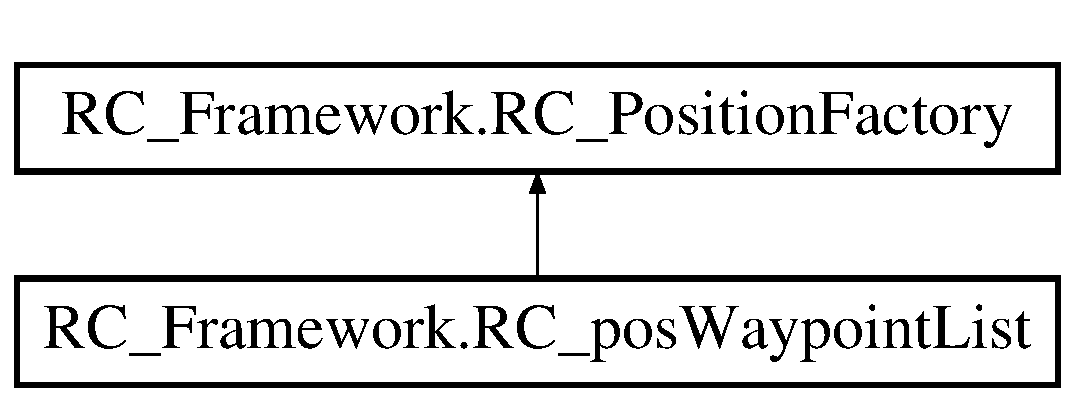
\includegraphics[height=2.000000cm]{class_r_c___framework_1_1_r_c__pos_waypoint_list}
\end{center}
\end{figure}
\subsection*{Public Member Functions}
\begin{DoxyCompactItemize}
\item 
\mbox{\hyperlink{class_r_c___framework_1_1_r_c__pos_waypoint_list_a25dad4f7211d21406f6d347c7ef8fda5}{R\+C\+\_\+pos\+Waypoint\+List}} (\mbox{\hyperlink{class_r_c___framework_1_1_way_point_list}{Way\+Point\+List}} w\+ListQ)
\item 
override Vector2 \mbox{\hyperlink{class_r_c___framework_1_1_r_c__pos_waypoint_list_a2f91d419c6513795cae3464fda807450}{get\+Next\+Pos}} ()
\item 
override void \mbox{\hyperlink{class_r_c___framework_1_1_r_c__pos_waypoint_list_a9bd29086f89fd9b6ad534dbf1d2785ab}{init}} ()
\item 
override void \mbox{\hyperlink{class_r_c___framework_1_1_r_c__pos_waypoint_list_acb5b5300a57cd6fc7c24db08bb27cdbf}{reset}} ()
\item 
override void \mbox{\hyperlink{class_r_c___framework_1_1_r_c__pos_waypoint_list_ae0bea3900f15e35e022f9b1d5c409067}{draw}} (Sprite\+Batch sb, Color col)
\end{DoxyCompactItemize}
\subsection*{Public Attributes}
\begin{DoxyCompactItemize}
\item 
\mbox{\hyperlink{class_r_c___framework_1_1_way_point_list}{Way\+Point\+List}} \mbox{\hyperlink{class_r_c___framework_1_1_r_c__pos_waypoint_list_a395db5f819084204a145fe2816b4937e}{w\+List}}
\end{DoxyCompactItemize}


\subsection{Detailed Description}
A class that takes a waypoint list and returns a set of positions 



\subsection{Constructor \& Destructor Documentation}
\mbox{\Hypertarget{class_r_c___framework_1_1_r_c__pos_waypoint_list_a25dad4f7211d21406f6d347c7ef8fda5}\label{class_r_c___framework_1_1_r_c__pos_waypoint_list_a25dad4f7211d21406f6d347c7ef8fda5}} 
\index{R\+C\+\_\+\+Framework\+::\+R\+C\+\_\+pos\+Waypoint\+List@{R\+C\+\_\+\+Framework\+::\+R\+C\+\_\+pos\+Waypoint\+List}!R\+C\+\_\+pos\+Waypoint\+List@{R\+C\+\_\+pos\+Waypoint\+List}}
\index{R\+C\+\_\+pos\+Waypoint\+List@{R\+C\+\_\+pos\+Waypoint\+List}!R\+C\+\_\+\+Framework\+::\+R\+C\+\_\+pos\+Waypoint\+List@{R\+C\+\_\+\+Framework\+::\+R\+C\+\_\+pos\+Waypoint\+List}}
\subsubsection{\texorpdfstring{R\+C\+\_\+pos\+Waypoint\+List()}{RC\_posWaypointList()}}
{\footnotesize\ttfamily R\+C\+\_\+\+Framework.\+R\+C\+\_\+pos\+Waypoint\+List.\+R\+C\+\_\+pos\+Waypoint\+List (\begin{DoxyParamCaption}\item[{\mbox{\hyperlink{class_r_c___framework_1_1_way_point_list}{Way\+Point\+List}}}]{w\+ListQ }\end{DoxyParamCaption})}



\subsection{Member Function Documentation}
\mbox{\Hypertarget{class_r_c___framework_1_1_r_c__pos_waypoint_list_ae0bea3900f15e35e022f9b1d5c409067}\label{class_r_c___framework_1_1_r_c__pos_waypoint_list_ae0bea3900f15e35e022f9b1d5c409067}} 
\index{R\+C\+\_\+\+Framework\+::\+R\+C\+\_\+pos\+Waypoint\+List@{R\+C\+\_\+\+Framework\+::\+R\+C\+\_\+pos\+Waypoint\+List}!draw@{draw}}
\index{draw@{draw}!R\+C\+\_\+\+Framework\+::\+R\+C\+\_\+pos\+Waypoint\+List@{R\+C\+\_\+\+Framework\+::\+R\+C\+\_\+pos\+Waypoint\+List}}
\subsubsection{\texorpdfstring{draw()}{draw()}}
{\footnotesize\ttfamily override void R\+C\+\_\+\+Framework.\+R\+C\+\_\+pos\+Waypoint\+List.\+draw (\begin{DoxyParamCaption}\item[{Sprite\+Batch}]{sb,  }\item[{Color}]{col }\end{DoxyParamCaption})\hspace{0.3cm}{\ttfamily [virtual]}}



Reimplemented from \mbox{\hyperlink{class_r_c___framework_1_1_r_c___position_factory_a39eaa0f4f1dfd07225b4880d494d81fa}{R\+C\+\_\+\+Framework.\+R\+C\+\_\+\+Position\+Factory}}.

\mbox{\Hypertarget{class_r_c___framework_1_1_r_c__pos_waypoint_list_a2f91d419c6513795cae3464fda807450}\label{class_r_c___framework_1_1_r_c__pos_waypoint_list_a2f91d419c6513795cae3464fda807450}} 
\index{R\+C\+\_\+\+Framework\+::\+R\+C\+\_\+pos\+Waypoint\+List@{R\+C\+\_\+\+Framework\+::\+R\+C\+\_\+pos\+Waypoint\+List}!get\+Next\+Pos@{get\+Next\+Pos}}
\index{get\+Next\+Pos@{get\+Next\+Pos}!R\+C\+\_\+\+Framework\+::\+R\+C\+\_\+pos\+Waypoint\+List@{R\+C\+\_\+\+Framework\+::\+R\+C\+\_\+pos\+Waypoint\+List}}
\subsubsection{\texorpdfstring{get\+Next\+Pos()}{getNextPos()}}
{\footnotesize\ttfamily override Vector2 R\+C\+\_\+\+Framework.\+R\+C\+\_\+pos\+Waypoint\+List.\+get\+Next\+Pos (\begin{DoxyParamCaption}{ }\end{DoxyParamCaption})\hspace{0.3cm}{\ttfamily [virtual]}}



Implements \mbox{\hyperlink{class_r_c___framework_1_1_r_c___position_factory_aab6cd4cb6a10c8dfa126c4930c6a9fbf}{R\+C\+\_\+\+Framework.\+R\+C\+\_\+\+Position\+Factory}}.

\mbox{\Hypertarget{class_r_c___framework_1_1_r_c__pos_waypoint_list_a9bd29086f89fd9b6ad534dbf1d2785ab}\label{class_r_c___framework_1_1_r_c__pos_waypoint_list_a9bd29086f89fd9b6ad534dbf1d2785ab}} 
\index{R\+C\+\_\+\+Framework\+::\+R\+C\+\_\+pos\+Waypoint\+List@{R\+C\+\_\+\+Framework\+::\+R\+C\+\_\+pos\+Waypoint\+List}!init@{init}}
\index{init@{init}!R\+C\+\_\+\+Framework\+::\+R\+C\+\_\+pos\+Waypoint\+List@{R\+C\+\_\+\+Framework\+::\+R\+C\+\_\+pos\+Waypoint\+List}}
\subsubsection{\texorpdfstring{init()}{init()}}
{\footnotesize\ttfamily override void R\+C\+\_\+\+Framework.\+R\+C\+\_\+pos\+Waypoint\+List.\+init (\begin{DoxyParamCaption}{ }\end{DoxyParamCaption})\hspace{0.3cm}{\ttfamily [virtual]}}



Reimplemented from \mbox{\hyperlink{class_r_c___framework_1_1_r_c___position_factory_af966db836e692a5a485531d227caa944}{R\+C\+\_\+\+Framework.\+R\+C\+\_\+\+Position\+Factory}}.

\mbox{\Hypertarget{class_r_c___framework_1_1_r_c__pos_waypoint_list_acb5b5300a57cd6fc7c24db08bb27cdbf}\label{class_r_c___framework_1_1_r_c__pos_waypoint_list_acb5b5300a57cd6fc7c24db08bb27cdbf}} 
\index{R\+C\+\_\+\+Framework\+::\+R\+C\+\_\+pos\+Waypoint\+List@{R\+C\+\_\+\+Framework\+::\+R\+C\+\_\+pos\+Waypoint\+List}!reset@{reset}}
\index{reset@{reset}!R\+C\+\_\+\+Framework\+::\+R\+C\+\_\+pos\+Waypoint\+List@{R\+C\+\_\+\+Framework\+::\+R\+C\+\_\+pos\+Waypoint\+List}}
\subsubsection{\texorpdfstring{reset()}{reset()}}
{\footnotesize\ttfamily override void R\+C\+\_\+\+Framework.\+R\+C\+\_\+pos\+Waypoint\+List.\+reset (\begin{DoxyParamCaption}{ }\end{DoxyParamCaption})\hspace{0.3cm}{\ttfamily [virtual]}}



Reimplemented from \mbox{\hyperlink{class_r_c___framework_1_1_r_c___position_factory_a582a8b01a360280d67b199b1190d96f7}{R\+C\+\_\+\+Framework.\+R\+C\+\_\+\+Position\+Factory}}.



\subsection{Member Data Documentation}
\mbox{\Hypertarget{class_r_c___framework_1_1_r_c__pos_waypoint_list_a395db5f819084204a145fe2816b4937e}\label{class_r_c___framework_1_1_r_c__pos_waypoint_list_a395db5f819084204a145fe2816b4937e}} 
\index{R\+C\+\_\+\+Framework\+::\+R\+C\+\_\+pos\+Waypoint\+List@{R\+C\+\_\+\+Framework\+::\+R\+C\+\_\+pos\+Waypoint\+List}!w\+List@{w\+List}}
\index{w\+List@{w\+List}!R\+C\+\_\+\+Framework\+::\+R\+C\+\_\+pos\+Waypoint\+List@{R\+C\+\_\+\+Framework\+::\+R\+C\+\_\+pos\+Waypoint\+List}}
\subsubsection{\texorpdfstring{w\+List}{wList}}
{\footnotesize\ttfamily \mbox{\hyperlink{class_r_c___framework_1_1_way_point_list}{Way\+Point\+List}} R\+C\+\_\+\+Framework.\+R\+C\+\_\+pos\+Waypoint\+List.\+w\+List}



The documentation for this class was generated from the following file\+:\begin{DoxyCompactItemize}
\item 
F\+:/\+B/\+R\+C\+\_\+\+Framework2018/\+Source/\mbox{\hyperlink{_r_c___position_factory_8cs}{R\+C\+\_\+\+Position\+Factory.\+cs}}\end{DoxyCompactItemize}

\hypertarget{class_r_c___framework_1_1_r_c__pos_x_y}{}\section{R\+C\+\_\+\+Framework.\+R\+C\+\_\+pos\+XY Class Reference}
\label{class_r_c___framework_1_1_r_c__pos_x_y}\index{R\+C\+\_\+\+Framework.\+R\+C\+\_\+pos\+XY@{R\+C\+\_\+\+Framework.\+R\+C\+\_\+pos\+XY}}


Creates positions which are just 1 position one x,y on the screen  


Inheritance diagram for R\+C\+\_\+\+Framework.\+R\+C\+\_\+pos\+XY\+:\begin{figure}[H]
\begin{center}
\leavevmode
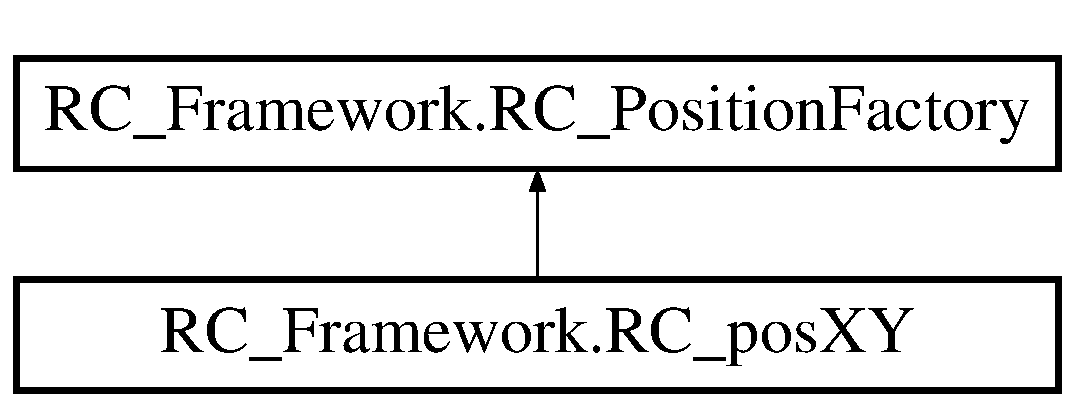
\includegraphics[height=2.000000cm]{class_r_c___framework_1_1_r_c__pos_x_y}
\end{center}
\end{figure}
\subsection*{Public Member Functions}
\begin{DoxyCompactItemize}
\item 
\mbox{\hyperlink{class_r_c___framework_1_1_r_c__pos_x_y_a27e517ab746a80cfaef66091813ad3ab}{R\+C\+\_\+pos\+XY}} (Vector2 posQ)
\item 
override Vector2 \mbox{\hyperlink{class_r_c___framework_1_1_r_c__pos_x_y_a773d0a5b2b6bfc49510dbecdfbf1f9cc}{get\+Next\+Pos}} ()
\item 
override void \mbox{\hyperlink{class_r_c___framework_1_1_r_c__pos_x_y_aaf344770b6a98b98937f4d43ffd536ef}{draw}} (Sprite\+Batch sb, Color col)
\end{DoxyCompactItemize}
\subsection*{Public Attributes}
\begin{DoxyCompactItemize}
\item 
Vector2 \mbox{\hyperlink{class_r_c___framework_1_1_r_c__pos_x_y_a4774a0f0a72a2c7bc38431e95df70b98}{poss}} = new Vector2(100, 100)
\end{DoxyCompactItemize}


\subsection{Detailed Description}
Creates positions which are just 1 position one x,y on the screen 



\subsection{Constructor \& Destructor Documentation}
\mbox{\Hypertarget{class_r_c___framework_1_1_r_c__pos_x_y_a27e517ab746a80cfaef66091813ad3ab}\label{class_r_c___framework_1_1_r_c__pos_x_y_a27e517ab746a80cfaef66091813ad3ab}} 
\index{R\+C\+\_\+\+Framework\+::\+R\+C\+\_\+pos\+XY@{R\+C\+\_\+\+Framework\+::\+R\+C\+\_\+pos\+XY}!R\+C\+\_\+pos\+XY@{R\+C\+\_\+pos\+XY}}
\index{R\+C\+\_\+pos\+XY@{R\+C\+\_\+pos\+XY}!R\+C\+\_\+\+Framework\+::\+R\+C\+\_\+pos\+XY@{R\+C\+\_\+\+Framework\+::\+R\+C\+\_\+pos\+XY}}
\subsubsection{\texorpdfstring{R\+C\+\_\+pos\+X\+Y()}{RC\_posXY()}}
{\footnotesize\ttfamily R\+C\+\_\+\+Framework.\+R\+C\+\_\+pos\+X\+Y.\+R\+C\+\_\+pos\+XY (\begin{DoxyParamCaption}\item[{Vector2}]{posQ }\end{DoxyParamCaption})}



\subsection{Member Function Documentation}
\mbox{\Hypertarget{class_r_c___framework_1_1_r_c__pos_x_y_aaf344770b6a98b98937f4d43ffd536ef}\label{class_r_c___framework_1_1_r_c__pos_x_y_aaf344770b6a98b98937f4d43ffd536ef}} 
\index{R\+C\+\_\+\+Framework\+::\+R\+C\+\_\+pos\+XY@{R\+C\+\_\+\+Framework\+::\+R\+C\+\_\+pos\+XY}!draw@{draw}}
\index{draw@{draw}!R\+C\+\_\+\+Framework\+::\+R\+C\+\_\+pos\+XY@{R\+C\+\_\+\+Framework\+::\+R\+C\+\_\+pos\+XY}}
\subsubsection{\texorpdfstring{draw()}{draw()}}
{\footnotesize\ttfamily override void R\+C\+\_\+\+Framework.\+R\+C\+\_\+pos\+X\+Y.\+draw (\begin{DoxyParamCaption}\item[{Sprite\+Batch}]{sb,  }\item[{Color}]{col }\end{DoxyParamCaption})\hspace{0.3cm}{\ttfamily [virtual]}}



Reimplemented from \mbox{\hyperlink{class_r_c___framework_1_1_r_c___position_factory_a39eaa0f4f1dfd07225b4880d494d81fa}{R\+C\+\_\+\+Framework.\+R\+C\+\_\+\+Position\+Factory}}.

\mbox{\Hypertarget{class_r_c___framework_1_1_r_c__pos_x_y_a773d0a5b2b6bfc49510dbecdfbf1f9cc}\label{class_r_c___framework_1_1_r_c__pos_x_y_a773d0a5b2b6bfc49510dbecdfbf1f9cc}} 
\index{R\+C\+\_\+\+Framework\+::\+R\+C\+\_\+pos\+XY@{R\+C\+\_\+\+Framework\+::\+R\+C\+\_\+pos\+XY}!get\+Next\+Pos@{get\+Next\+Pos}}
\index{get\+Next\+Pos@{get\+Next\+Pos}!R\+C\+\_\+\+Framework\+::\+R\+C\+\_\+pos\+XY@{R\+C\+\_\+\+Framework\+::\+R\+C\+\_\+pos\+XY}}
\subsubsection{\texorpdfstring{get\+Next\+Pos()}{getNextPos()}}
{\footnotesize\ttfamily override Vector2 R\+C\+\_\+\+Framework.\+R\+C\+\_\+pos\+X\+Y.\+get\+Next\+Pos (\begin{DoxyParamCaption}{ }\end{DoxyParamCaption})\hspace{0.3cm}{\ttfamily [virtual]}}



Implements \mbox{\hyperlink{class_r_c___framework_1_1_r_c___position_factory_aab6cd4cb6a10c8dfa126c4930c6a9fbf}{R\+C\+\_\+\+Framework.\+R\+C\+\_\+\+Position\+Factory}}.



\subsection{Member Data Documentation}
\mbox{\Hypertarget{class_r_c___framework_1_1_r_c__pos_x_y_a4774a0f0a72a2c7bc38431e95df70b98}\label{class_r_c___framework_1_1_r_c__pos_x_y_a4774a0f0a72a2c7bc38431e95df70b98}} 
\index{R\+C\+\_\+\+Framework\+::\+R\+C\+\_\+pos\+XY@{R\+C\+\_\+\+Framework\+::\+R\+C\+\_\+pos\+XY}!poss@{poss}}
\index{poss@{poss}!R\+C\+\_\+\+Framework\+::\+R\+C\+\_\+pos\+XY@{R\+C\+\_\+\+Framework\+::\+R\+C\+\_\+pos\+XY}}
\subsubsection{\texorpdfstring{poss}{poss}}
{\footnotesize\ttfamily Vector2 R\+C\+\_\+\+Framework.\+R\+C\+\_\+pos\+X\+Y.\+poss = new Vector2(100, 100)}



The documentation for this class was generated from the following file\+:\begin{DoxyCompactItemize}
\item 
F\+:/\+B/\+R\+C\+\_\+\+Framework2018/\+Source/\mbox{\hyperlink{_r_c___position_factory_8cs}{R\+C\+\_\+\+Position\+Factory.\+cs}}\end{DoxyCompactItemize}

\hypertarget{class_r_c___framework_1_1_r_c___renderable}{}\section{R\+C\+\_\+\+Framework.\+R\+C\+\_\+\+Renderable Class Reference}
\label{class_r_c___framework_1_1_r_c___renderable}\index{R\+C\+\_\+\+Framework.\+R\+C\+\_\+\+Renderable@{R\+C\+\_\+\+Framework.\+R\+C\+\_\+\+Renderable}}


Parent class for all renderables sprites and list of things to draw has active flag, color, and visible properties and draw, load contenet and update functions also mouse and keyhit functions  


Inheritance diagram for R\+C\+\_\+\+Framework.\+R\+C\+\_\+\+Renderable\+:\begin{figure}[H]
\begin{center}
\leavevmode
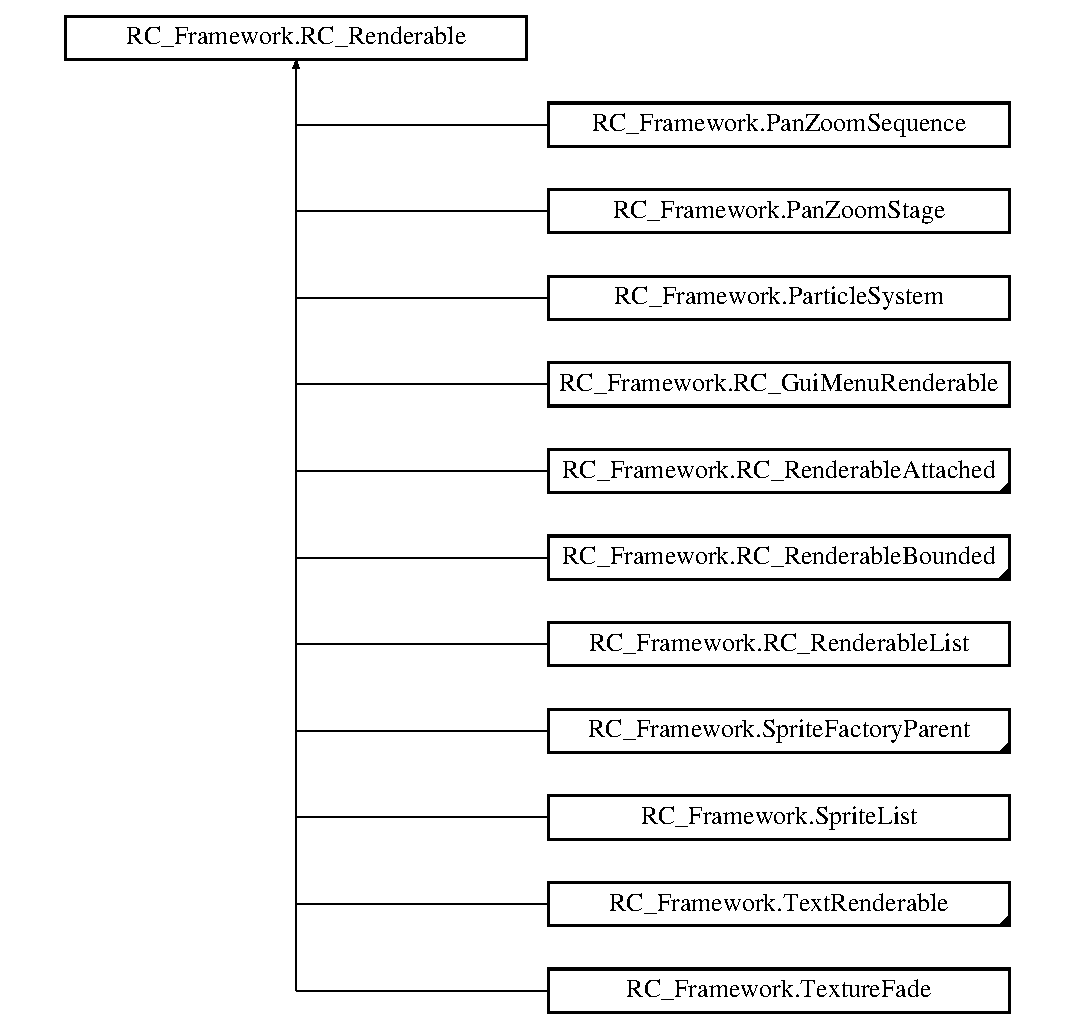
\includegraphics[height=12.000000cm]{class_r_c___framework_1_1_r_c___renderable}
\end{center}
\end{figure}
\subsection*{Public Member Functions}
\begin{DoxyCompactItemize}
\item 
\mbox{\hyperlink{class_r_c___framework_1_1_r_c___renderable_af2c1d0e50a166ca2bd5137dafc7ab105}{R\+C\+\_\+\+Renderable}} ()
\begin{DoxyCompactList}\small\item\em a default constructor \end{DoxyCompactList}\item 
\mbox{\hyperlink{class_r_c___framework_1_1_r_c___renderable_a2f171037bc65e22991e1e4d32ecd8154}{R\+C\+\_\+\+Renderable}} (bool activeZ, bool visibleZ, Color colorZ)
\begin{DoxyCompactList}\small\item\em a more usefull constructor \end{DoxyCompactList}\item 
\mbox{\hyperlink{class_r_c___framework_1_1_r_c___renderable_aa5848d536a2dd1d0c8269a9ea48a06fb}{R\+C\+\_\+\+Renderable}} (\mbox{\hyperlink{class_r_c___framework_1_1_r_c___renderable}{R\+C\+\_\+\+Renderable}} r)
\begin{DoxyCompactList}\small\item\em Copy constructor dont know if it will ever be used since its a parent class \end{DoxyCompactList}\item 
virtual void \mbox{\hyperlink{class_r_c___framework_1_1_r_c___renderable_a73bf15681dc31644705e509c53f68833}{set\+Color}} (Color c)
\begin{DoxyCompactList}\small\item\em Sets the blend colour for the sprite if in doubt use Color.\+White \end{DoxyCompactList}\item 
Color \mbox{\hyperlink{class_r_c___framework_1_1_r_c___renderable_a4066c494d71a398ce2dfb6b932027243}{get\+Color}} ()
\begin{DoxyCompactList}\small\item\em Gets the sprite blend colour \end{DoxyCompactList}\item 
virtual void \mbox{\hyperlink{class_r_c___framework_1_1_r_c___renderable_acc26db34e382a25a989c4c0dd0354b23}{Draw}} (Sprite\+Batch sb)
\begin{DoxyCompactList}\small\item\em Standard draw routine which assumes the renderable knows where it is \end{DoxyCompactList}\item 
virtual void \mbox{\hyperlink{class_r_c___framework_1_1_r_c___renderable_a5745bedc7ba0587aa1e1d8563c357228}{Update}} (Game\+Time game\+Time)
\item 
virtual void \mbox{\hyperlink{class_r_c___framework_1_1_r_c___renderable_ae5283e88f2cc34c2ef010ede22ab1bfb}{Load\+Content}} ()
\item 
virtual void \mbox{\hyperlink{class_r_c___framework_1_1_r_c___renderable_ae65ce69704d15963789f421b58618b1f}{reset}} ()
\item 
void \mbox{\hyperlink{class_r_c___framework_1_1_r_c___renderable_a3fc6f1efc5735fb15ad0a02b1b821a62}{set\+Visible}} (bool v)
\begin{DoxyCompactList}\small\item\em Set if the renderable is visible \end{DoxyCompactList}\item 
bool \mbox{\hyperlink{class_r_c___framework_1_1_r_c___renderable_a6258a044f185b02adb80d441fd9f29b2}{get\+Visible}} ()
\begin{DoxyCompactList}\small\item\em Um this should be obvious \end{DoxyCompactList}\item 
virtual bool \mbox{\hyperlink{class_r_c___framework_1_1_r_c___renderable_a21e5b1a68c7382443c82e7296fd2209a}{scroll\+Move}} (float x, float y)
\begin{DoxyCompactList}\small\item\em Used to scroll the entire screen -\/ in renderable simple but increases in complexity as the parent child tree deepens (eg sprite3) \end{DoxyCompactList}\item 
virtual bool \mbox{\hyperlink{class_r_c___framework_1_1_r_c___renderable_a64771aae3018662ed596c01ee36fb87f}{Mouse\+Move\+Event}} (Mouse\+State ms, Mouse\+State previous\+Ms)
\begin{DoxyCompactList}\small\item\em Events in the this class can be consumed so default behavious must be to return false this will indicate that the event was not consumed \end{DoxyCompactList}\item 
virtual bool \mbox{\hyperlink{class_r_c___framework_1_1_r_c___renderable_a41d144d6fad27f219d861e61a2d9796e}{Mouse\+Down\+Event\+Left}} (float mouse\+\_\+x, float mouse\+\_\+y)
\item 
virtual bool \mbox{\hyperlink{class_r_c___framework_1_1_r_c___renderable_a9545f4486eacd645e0c6680976020950}{Mouse\+Up\+Event\+Left}} (float mouse\+\_\+x, float mouse\+\_\+y)
\item 
virtual bool \mbox{\hyperlink{class_r_c___framework_1_1_r_c___renderable_a827d6c2bde928d9337b341f2ff60ac48}{Mouse\+Down\+Event\+Right}} (float mouse\+\_\+x, float mouse\+\_\+y)
\item 
virtual bool \mbox{\hyperlink{class_r_c___framework_1_1_r_c___renderable_afd14f09a6249144be45af3dcb9ebe1b2}{Mouse\+Up\+Event\+Right}} (float mouse\+\_\+x, float mouse\+\_\+y)
\item 
virtual bool \mbox{\hyperlink{class_r_c___framework_1_1_r_c___renderable_af929e80b7c88bb21b01358f47ad36a64}{Mouse\+Click\+Event}} (float mouse\+\_\+x, float mouse\+\_\+y)
\item 
virtual bool \mbox{\hyperlink{class_r_c___framework_1_1_r_c___renderable_a826da9b07316c475186e4c2f00648827}{Key\+Hit\+Event}} (Keys key\+Hit)
\item 
virtual bool \mbox{\hyperlink{class_r_c___framework_1_1_r_c___renderable_abd55ea96d88d7bd2207e3a4ede1f1a05}{Mouse\+Over}} (float mouse\+\_\+x, float mouse\+\_\+y)
\end{DoxyCompactItemize}
\subsection*{Public Attributes}
\begin{DoxyCompactItemize}
\item 
string \mbox{\hyperlink{class_r_c___framework_1_1_r_c___renderable_a255c5d9294a719e56855890f3535d129}{text}} = \char`\"{}\char`\"{}
\begin{DoxyCompactList}\small\item\em This variable called text is just for users to attach a string to the renderable or sprite it is used by the attached renderable \mbox{\hyperlink{class_r_c___framework_1_1_attached_text}{Attached\+Text}} and some other renderables (eg text ones and buttons) \end{DoxyCompactList}\end{DoxyCompactItemize}
\subsection*{Properties}
\begin{DoxyCompactItemize}
\item 
bool \mbox{\hyperlink{class_r_c___framework_1_1_r_c___renderable_a192f8ec61fb5e94770fcb3a1f9ae3449}{active}}\hspace{0.3cm}{\ttfamily  \mbox{[}get, set\mbox{]}}
\begin{DoxyCompactList}\small\item\em this variable called active is used by things like renderable\+\_\+list, sprite\+\_\+list and gui\+\_\+list if a renderable is not active it means it can be deleted or overwritten it is used in conjunction with sprite list to manage activity of sprites in a list importantly inactive renderables should not be given Draw or update (or other UI) events \end{DoxyCompactList}\item 
Color \mbox{\hyperlink{class_r_c___framework_1_1_r_c___renderable_ad2731b86927b47a6f661f18446332afc}{colour}}\hspace{0.3cm}{\ttfamily  \mbox{[}get, set\mbox{]}}
\begin{DoxyCompactList}\small\item\em This is the render colour its usually pushed into the spritebatch draw unchanged \end{DoxyCompactList}\item 
bool \mbox{\hyperlink{class_r_c___framework_1_1_r_c___renderable_a27490992e58f8295c86cd3ed1d79d937}{visible}}\hspace{0.3cm}{\ttfamily  \mbox{[}get, set\mbox{]}}
\begin{DoxyCompactList}\small\item\em is it visible \end{DoxyCompactList}\item 
float \mbox{\hyperlink{class_r_c___framework_1_1_r_c___renderable_a892d384578d86317fc3975ce977f89ef}{tag}}\hspace{0.3cm}{\ttfamily  \mbox{[}get, set\mbox{]}}
\begin{DoxyCompactList}\small\item\em this variable called tag is available for use by user code \end{DoxyCompactList}\item 
int \mbox{\hyperlink{class_r_c___framework_1_1_r_c___renderable_ab429caeeb6b5ce111036e1828b5b3777}{tag\+Int}}\hspace{0.3cm}{\ttfamily  \mbox{[}get, set\mbox{]}}
\begin{DoxyCompactList}\small\item\em this variable called tag\+Int is available for use by user code \end{DoxyCompactList}\end{DoxyCompactItemize}


\subsection{Detailed Description}
Parent class for all renderables sprites and list of things to draw has active flag, color, and visible properties and draw, load contenet and update functions also mouse and keyhit functions 

Recently added tag and tag\+Int to help making general purpose renderables 

\subsection{Constructor \& Destructor Documentation}
\mbox{\Hypertarget{class_r_c___framework_1_1_r_c___renderable_af2c1d0e50a166ca2bd5137dafc7ab105}\label{class_r_c___framework_1_1_r_c___renderable_af2c1d0e50a166ca2bd5137dafc7ab105}} 
\index{R\+C\+\_\+\+Framework\+::\+R\+C\+\_\+\+Renderable@{R\+C\+\_\+\+Framework\+::\+R\+C\+\_\+\+Renderable}!R\+C\+\_\+\+Renderable@{R\+C\+\_\+\+Renderable}}
\index{R\+C\+\_\+\+Renderable@{R\+C\+\_\+\+Renderable}!R\+C\+\_\+\+Framework\+::\+R\+C\+\_\+\+Renderable@{R\+C\+\_\+\+Framework\+::\+R\+C\+\_\+\+Renderable}}
\subsubsection{\texorpdfstring{R\+C\+\_\+\+Renderable()}{RC\_Renderable()}\hspace{0.1cm}{\footnotesize\ttfamily [1/3]}}
{\footnotesize\ttfamily R\+C\+\_\+\+Framework.\+R\+C\+\_\+\+Renderable.\+R\+C\+\_\+\+Renderable (\begin{DoxyParamCaption}{ }\end{DoxyParamCaption})}



a default constructor 

\mbox{\Hypertarget{class_r_c___framework_1_1_r_c___renderable_a2f171037bc65e22991e1e4d32ecd8154}\label{class_r_c___framework_1_1_r_c___renderable_a2f171037bc65e22991e1e4d32ecd8154}} 
\index{R\+C\+\_\+\+Framework\+::\+R\+C\+\_\+\+Renderable@{R\+C\+\_\+\+Framework\+::\+R\+C\+\_\+\+Renderable}!R\+C\+\_\+\+Renderable@{R\+C\+\_\+\+Renderable}}
\index{R\+C\+\_\+\+Renderable@{R\+C\+\_\+\+Renderable}!R\+C\+\_\+\+Framework\+::\+R\+C\+\_\+\+Renderable@{R\+C\+\_\+\+Framework\+::\+R\+C\+\_\+\+Renderable}}
\subsubsection{\texorpdfstring{R\+C\+\_\+\+Renderable()}{RC\_Renderable()}\hspace{0.1cm}{\footnotesize\ttfamily [2/3]}}
{\footnotesize\ttfamily R\+C\+\_\+\+Framework.\+R\+C\+\_\+\+Renderable.\+R\+C\+\_\+\+Renderable (\begin{DoxyParamCaption}\item[{bool}]{activeZ,  }\item[{bool}]{visibleZ,  }\item[{Color}]{colorZ }\end{DoxyParamCaption})}



a more usefull constructor 


\begin{DoxyParams}{Parameters}
{\em activeZ} & \\
\hline
{\em visibleZ} & \\
\hline
{\em colorZ} & \\
\hline
\end{DoxyParams}
\mbox{\Hypertarget{class_r_c___framework_1_1_r_c___renderable_aa5848d536a2dd1d0c8269a9ea48a06fb}\label{class_r_c___framework_1_1_r_c___renderable_aa5848d536a2dd1d0c8269a9ea48a06fb}} 
\index{R\+C\+\_\+\+Framework\+::\+R\+C\+\_\+\+Renderable@{R\+C\+\_\+\+Framework\+::\+R\+C\+\_\+\+Renderable}!R\+C\+\_\+\+Renderable@{R\+C\+\_\+\+Renderable}}
\index{R\+C\+\_\+\+Renderable@{R\+C\+\_\+\+Renderable}!R\+C\+\_\+\+Framework\+::\+R\+C\+\_\+\+Renderable@{R\+C\+\_\+\+Framework\+::\+R\+C\+\_\+\+Renderable}}
\subsubsection{\texorpdfstring{R\+C\+\_\+\+Renderable()}{RC\_Renderable()}\hspace{0.1cm}{\footnotesize\ttfamily [3/3]}}
{\footnotesize\ttfamily R\+C\+\_\+\+Framework.\+R\+C\+\_\+\+Renderable.\+R\+C\+\_\+\+Renderable (\begin{DoxyParamCaption}\item[{\mbox{\hyperlink{class_r_c___framework_1_1_r_c___renderable}{R\+C\+\_\+\+Renderable}}}]{r }\end{DoxyParamCaption})}



Copy constructor dont know if it will ever be used since its a parent class 



\subsection{Member Function Documentation}
\mbox{\Hypertarget{class_r_c___framework_1_1_r_c___renderable_acc26db34e382a25a989c4c0dd0354b23}\label{class_r_c___framework_1_1_r_c___renderable_acc26db34e382a25a989c4c0dd0354b23}} 
\index{R\+C\+\_\+\+Framework\+::\+R\+C\+\_\+\+Renderable@{R\+C\+\_\+\+Framework\+::\+R\+C\+\_\+\+Renderable}!Draw@{Draw}}
\index{Draw@{Draw}!R\+C\+\_\+\+Framework\+::\+R\+C\+\_\+\+Renderable@{R\+C\+\_\+\+Framework\+::\+R\+C\+\_\+\+Renderable}}
\subsubsection{\texorpdfstring{Draw()}{Draw()}}
{\footnotesize\ttfamily virtual void R\+C\+\_\+\+Framework.\+R\+C\+\_\+\+Renderable.\+Draw (\begin{DoxyParamCaption}\item[{Sprite\+Batch}]{sb }\end{DoxyParamCaption})\hspace{0.3cm}{\ttfamily [virtual]}}



Standard draw routine which assumes the renderable knows where it is 


\begin{DoxyParams}{Parameters}
{\em sb} & \\
\hline
\end{DoxyParams}


Reimplemented in \mbox{\hyperlink{class_r_c___framework_1_1_sprite3_a79b8e18ee29cd62719307a059e4cb6df}{R\+C\+\_\+\+Framework.\+Sprite3}}, \mbox{\hyperlink{class_r_c___framework_1_1_string_list_box_a474da32176236c6a1f36129c8cac0386}{R\+C\+\_\+\+Framework.\+String\+List\+Box}}, \mbox{\hyperlink{class_r_c___framework_1_1_texture_flash_1_1_letterbox_mask_aadd01ce0789efac12bc044f336bb5b33}{R\+C\+\_\+\+Framework.\+Texture\+Flash.\+Letterbox\+Mask}}, \mbox{\hyperlink{class_r_c___framework_1_1_texture_flash_a37d7b37ad7c1816d6cf967ad784c7d0f}{R\+C\+\_\+\+Framework.\+Texture\+Flash}}, \mbox{\hyperlink{class_r_c___framework_1_1_input_box_ae5ee048852636d3675318a630cfc0ec6}{R\+C\+\_\+\+Framework.\+Input\+Box}}, \mbox{\hyperlink{class_r_c___framework_1_1_grid_back_ground_a242904271618f793025f4dfae9681c13}{R\+C\+\_\+\+Framework.\+Grid\+Back\+Ground}}, \mbox{\hyperlink{class_r_c___framework_1_1_image_background_a1aaef38a9b320b21dc558e25d5a4c0af}{R\+C\+\_\+\+Framework.\+Image\+Background}}, \mbox{\hyperlink{class_r_c___framework_1_1_text_box_a4a237df7322d0a902b7c5144b0c7bf0d}{R\+C\+\_\+\+Framework.\+Text\+Box}}, \mbox{\hyperlink{class_r_c___framework_1_1_repeat_image_ad0d9de5911c47f93d7ed1dc48f531283}{R\+C\+\_\+\+Framework.\+Repeat\+Image}}, \mbox{\hyperlink{class_r_c___framework_1_1_button_s_i_a9527749f48994c13be5b72b2cb370b29}{R\+C\+\_\+\+Framework.\+Button\+SI}}, \mbox{\hyperlink{class_r_c___framework_1_1_blinking_boxes_a4e8a5e543c03905582bb27a0acfaa6cd}{R\+C\+\_\+\+Framework.\+Blinking\+Boxes}}, \mbox{\hyperlink{class_r_c___framework_1_1_renderable_frame_af07cf299871051c7e1c6ca455ba1bab9}{R\+C\+\_\+\+Framework.\+Renderable\+Frame}}, \mbox{\hyperlink{class_r_c___framework_1_1_button2_addc2770e16ca29d6bad27e7b234dddf3}{R\+C\+\_\+\+Framework.\+Button2}}, \mbox{\hyperlink{class_r_c___framework_1_1_particle_system_a2cb9a22f944e93697fff3128a1d3ddb6}{R\+C\+\_\+\+Framework.\+Particle\+System}}, \mbox{\hyperlink{class_r_c___framework_1_1_frame_ac27d7d9f33b34045c4dc90287f3eacee}{R\+C\+\_\+\+Framework.\+Frame}}, \mbox{\hyperlink{class_r_c___framework_1_1_scroll_back_ground_a7b9513679627c90648d41b952d4231d1}{R\+C\+\_\+\+Framework.\+Scroll\+Back\+Ground}}, \mbox{\hyperlink{class_r_c___framework_1_1_circle_fade_a75194b070e20dab4a4720c9ba43ae5ab}{R\+C\+\_\+\+Framework.\+Circle\+Fade}}, \mbox{\hyperlink{class_r_c___framework_1_1_sprite_list_a4100c8d4abaa1e7268c17607d70b539a}{R\+C\+\_\+\+Framework.\+Sprite\+List}}, \mbox{\hyperlink{class_r_c___framework_1_1_text_renderable_flash_ac917a0d6ed0b003f6565a7e822b517ba}{R\+C\+\_\+\+Framework.\+Text\+Renderable\+Flash}}, \mbox{\hyperlink{class_r_c___framework_1_1test_texture_list_ad9d3cd0a926c420d493e2a92fdadcab1}{R\+C\+\_\+\+Framework.\+test\+Texture\+List}}, \mbox{\hyperlink{class_r_c___framework_1_1_pan_zoom_sequence_a63516b58108ff5f5bcb03d24230128f3}{R\+C\+\_\+\+Framework.\+Pan\+Zoom\+Sequence}}, \mbox{\hyperlink{class_r_c___framework_1_1_text_renderable_fade_a6c0562ac01be810eb4e81f3f81e21bbd}{R\+C\+\_\+\+Framework.\+Text\+Renderable\+Fade}}, \mbox{\hyperlink{class_r_c___framework_1_1_attached_texture_fade_a93612655099524c9059b6ae9437bda59}{R\+C\+\_\+\+Framework.\+Attached\+Texture\+Fade}}, \mbox{\hyperlink{class_r_c___framework_1_1_r_c___renderable_list_a274ae54ac48b42415db6b3193587e8d4}{R\+C\+\_\+\+Framework.\+R\+C\+\_\+\+Renderable\+List}}, \mbox{\hyperlink{class_r_c___framework_1_1_button_ann_ab513dd55d4cf3e1515761f0e4c5f9e44}{R\+C\+\_\+\+Framework.\+Button\+Ann}}, \mbox{\hyperlink{class_r_c___framework_1_1_multi_renderable_ae81e6924e30c2ff36c5b13204f3d2857}{R\+C\+\_\+\+Framework.\+Multi\+Renderable}}, \mbox{\hyperlink{class_r_c___framework_1_1_attached_text_a5972b29f469c9c005a46652ab448411c}{R\+C\+\_\+\+Framework.\+Attached\+Text}}, \mbox{\hyperlink{class_r_c___framework_1_1_texture_fade_ac5e515a49540f0609de47ba2f36ddc51}{R\+C\+\_\+\+Framework.\+Texture\+Fade}}, \mbox{\hyperlink{class_r_c___framework_1_1_r_c___gui_menu_renderable_a0c74b42e4af1cad77f708cfa174aa724}{R\+C\+\_\+\+Framework.\+R\+C\+\_\+\+Gui\+Menu\+Renderable}}, \mbox{\hyperlink{class_r_c___framework_1_1_text_renderable_bordered_a3242eaa3191281834da585239048f8ce}{R\+C\+\_\+\+Framework.\+Text\+Renderable\+Bordered}}, \mbox{\hyperlink{class_r_c___framework_1_1_pan_zoom_stage_a399538cd702d22cb14394f73b1bccff6}{R\+C\+\_\+\+Framework.\+Pan\+Zoom\+Stage}}, \mbox{\hyperlink{class_r_c___framework_1_1_multi_scroll_back_ground_ac59e7e1e7a2e1ccfc364883b98765f00}{R\+C\+\_\+\+Framework.\+Multi\+Scroll\+Back\+Ground}}, \mbox{\hyperlink{class_r_c___framework_1_1_r_c__resize_text_aa591010e25943e1c1a45555cecaa8fcc}{R\+C\+\_\+\+Framework.\+R\+C\+\_\+resize\+Text}}, \mbox{\hyperlink{class_r_c___framework_1_1_health_bar_a8f53c56c52544e3c257db3d698fd2926}{R\+C\+\_\+\+Framework.\+Health\+Bar}}, \mbox{\hyperlink{class_r_c___framework_1_1_text_renderable_aea36ff48ac5dc6a336d998111457f019}{R\+C\+\_\+\+Framework.\+Text\+Renderable}}, and \mbox{\hyperlink{class_r_c___framework_1_1_color_field_a431503895c3a851dc8ca6586dd4686fe}{R\+C\+\_\+\+Framework.\+Color\+Field}}.

\mbox{\Hypertarget{class_r_c___framework_1_1_r_c___renderable_a4066c494d71a398ce2dfb6b932027243}\label{class_r_c___framework_1_1_r_c___renderable_a4066c494d71a398ce2dfb6b932027243}} 
\index{R\+C\+\_\+\+Framework\+::\+R\+C\+\_\+\+Renderable@{R\+C\+\_\+\+Framework\+::\+R\+C\+\_\+\+Renderable}!get\+Color@{get\+Color}}
\index{get\+Color@{get\+Color}!R\+C\+\_\+\+Framework\+::\+R\+C\+\_\+\+Renderable@{R\+C\+\_\+\+Framework\+::\+R\+C\+\_\+\+Renderable}}
\subsubsection{\texorpdfstring{get\+Color()}{getColor()}}
{\footnotesize\ttfamily Color R\+C\+\_\+\+Framework.\+R\+C\+\_\+\+Renderable.\+get\+Color (\begin{DoxyParamCaption}{ }\end{DoxyParamCaption})}



Gets the sprite blend colour 

\begin{DoxyReturn}{Returns}

\end{DoxyReturn}
\mbox{\Hypertarget{class_r_c___framework_1_1_r_c___renderable_a6258a044f185b02adb80d441fd9f29b2}\label{class_r_c___framework_1_1_r_c___renderable_a6258a044f185b02adb80d441fd9f29b2}} 
\index{R\+C\+\_\+\+Framework\+::\+R\+C\+\_\+\+Renderable@{R\+C\+\_\+\+Framework\+::\+R\+C\+\_\+\+Renderable}!get\+Visible@{get\+Visible}}
\index{get\+Visible@{get\+Visible}!R\+C\+\_\+\+Framework\+::\+R\+C\+\_\+\+Renderable@{R\+C\+\_\+\+Framework\+::\+R\+C\+\_\+\+Renderable}}
\subsubsection{\texorpdfstring{get\+Visible()}{getVisible()}}
{\footnotesize\ttfamily bool R\+C\+\_\+\+Framework.\+R\+C\+\_\+\+Renderable.\+get\+Visible (\begin{DoxyParamCaption}{ }\end{DoxyParamCaption})}



Um this should be obvious 

\begin{DoxyReturn}{Returns}

\end{DoxyReturn}
\mbox{\Hypertarget{class_r_c___framework_1_1_r_c___renderable_a826da9b07316c475186e4c2f00648827}\label{class_r_c___framework_1_1_r_c___renderable_a826da9b07316c475186e4c2f00648827}} 
\index{R\+C\+\_\+\+Framework\+::\+R\+C\+\_\+\+Renderable@{R\+C\+\_\+\+Framework\+::\+R\+C\+\_\+\+Renderable}!Key\+Hit\+Event@{Key\+Hit\+Event}}
\index{Key\+Hit\+Event@{Key\+Hit\+Event}!R\+C\+\_\+\+Framework\+::\+R\+C\+\_\+\+Renderable@{R\+C\+\_\+\+Framework\+::\+R\+C\+\_\+\+Renderable}}
\subsubsection{\texorpdfstring{Key\+Hit\+Event()}{KeyHitEvent()}}
{\footnotesize\ttfamily virtual bool R\+C\+\_\+\+Framework.\+R\+C\+\_\+\+Renderable.\+Key\+Hit\+Event (\begin{DoxyParamCaption}\item[{Keys}]{key\+Hit }\end{DoxyParamCaption})\hspace{0.3cm}{\ttfamily [virtual]}}



Reimplemented in \mbox{\hyperlink{class_r_c___framework_1_1_string_list_box_a8b449ef1c2c786786b7e6cf52f416750}{R\+C\+\_\+\+Framework.\+String\+List\+Box}}, \mbox{\hyperlink{class_r_c___framework_1_1_input_box_a07ef881a281e4da95994e54ec1f7b496}{R\+C\+\_\+\+Framework.\+Input\+Box}}, \mbox{\hyperlink{class_r_c___framework_1_1_text_box_ae8c28e507b2c91aa042e2a5c2a300598}{R\+C\+\_\+\+Framework.\+Text\+Box}}, \mbox{\hyperlink{class_r_c___framework_1_1_r_c___renderable_list_a221a0bf056ff4f8e02d22e3b8b66de81}{R\+C\+\_\+\+Framework.\+R\+C\+\_\+\+Renderable\+List}}, \mbox{\hyperlink{class_r_c___framework_1_1_g_u_i___control_a458eb00bda180db22ebe22e550a669a4}{R\+C\+\_\+\+Framework.\+G\+U\+I\+\_\+\+Control}}, and \mbox{\hyperlink{class_r_c___framework_1_1_r_c___gui_menu_renderable_a2a1be820f5693b0badd408b5457c81bd}{R\+C\+\_\+\+Framework.\+R\+C\+\_\+\+Gui\+Menu\+Renderable}}.

\mbox{\Hypertarget{class_r_c___framework_1_1_r_c___renderable_ae5283e88f2cc34c2ef010ede22ab1bfb}\label{class_r_c___framework_1_1_r_c___renderable_ae5283e88f2cc34c2ef010ede22ab1bfb}} 
\index{R\+C\+\_\+\+Framework\+::\+R\+C\+\_\+\+Renderable@{R\+C\+\_\+\+Framework\+::\+R\+C\+\_\+\+Renderable}!Load\+Content@{Load\+Content}}
\index{Load\+Content@{Load\+Content}!R\+C\+\_\+\+Framework\+::\+R\+C\+\_\+\+Renderable@{R\+C\+\_\+\+Framework\+::\+R\+C\+\_\+\+Renderable}}
\subsubsection{\texorpdfstring{Load\+Content()}{LoadContent()}}
{\footnotesize\ttfamily virtual void R\+C\+\_\+\+Framework.\+R\+C\+\_\+\+Renderable.\+Load\+Content (\begin{DoxyParamCaption}{ }\end{DoxyParamCaption})\hspace{0.3cm}{\ttfamily [virtual]}}



Reimplemented in \mbox{\hyperlink{class_r_c___framework_1_1_r_c___renderable_list_a953e8eb6f4422a7f0bebb17ee0455c42}{R\+C\+\_\+\+Framework.\+R\+C\+\_\+\+Renderable\+List}}.

\mbox{\Hypertarget{class_r_c___framework_1_1_r_c___renderable_af929e80b7c88bb21b01358f47ad36a64}\label{class_r_c___framework_1_1_r_c___renderable_af929e80b7c88bb21b01358f47ad36a64}} 
\index{R\+C\+\_\+\+Framework\+::\+R\+C\+\_\+\+Renderable@{R\+C\+\_\+\+Framework\+::\+R\+C\+\_\+\+Renderable}!Mouse\+Click\+Event@{Mouse\+Click\+Event}}
\index{Mouse\+Click\+Event@{Mouse\+Click\+Event}!R\+C\+\_\+\+Framework\+::\+R\+C\+\_\+\+Renderable@{R\+C\+\_\+\+Framework\+::\+R\+C\+\_\+\+Renderable}}
\subsubsection{\texorpdfstring{Mouse\+Click\+Event()}{MouseClickEvent()}}
{\footnotesize\ttfamily virtual bool R\+C\+\_\+\+Framework.\+R\+C\+\_\+\+Renderable.\+Mouse\+Click\+Event (\begin{DoxyParamCaption}\item[{float}]{mouse\+\_\+x,  }\item[{float}]{mouse\+\_\+y }\end{DoxyParamCaption})\hspace{0.3cm}{\ttfamily [virtual]}}



Reimplemented in \mbox{\hyperlink{class_r_c___framework_1_1_r_c___renderable_list_ac275d3df45899b62e1378e01a100268d}{R\+C\+\_\+\+Framework.\+R\+C\+\_\+\+Renderable\+List}}, and \mbox{\hyperlink{class_r_c___framework_1_1_r_c___gui_menu_renderable_a211b5eebda9524d97f8dfeb1f8024f32}{R\+C\+\_\+\+Framework.\+R\+C\+\_\+\+Gui\+Menu\+Renderable}}.

\mbox{\Hypertarget{class_r_c___framework_1_1_r_c___renderable_a41d144d6fad27f219d861e61a2d9796e}\label{class_r_c___framework_1_1_r_c___renderable_a41d144d6fad27f219d861e61a2d9796e}} 
\index{R\+C\+\_\+\+Framework\+::\+R\+C\+\_\+\+Renderable@{R\+C\+\_\+\+Framework\+::\+R\+C\+\_\+\+Renderable}!Mouse\+Down\+Event\+Left@{Mouse\+Down\+Event\+Left}}
\index{Mouse\+Down\+Event\+Left@{Mouse\+Down\+Event\+Left}!R\+C\+\_\+\+Framework\+::\+R\+C\+\_\+\+Renderable@{R\+C\+\_\+\+Framework\+::\+R\+C\+\_\+\+Renderable}}
\subsubsection{\texorpdfstring{Mouse\+Down\+Event\+Left()}{MouseDownEventLeft()}}
{\footnotesize\ttfamily virtual bool R\+C\+\_\+\+Framework.\+R\+C\+\_\+\+Renderable.\+Mouse\+Down\+Event\+Left (\begin{DoxyParamCaption}\item[{float}]{mouse\+\_\+x,  }\item[{float}]{mouse\+\_\+y }\end{DoxyParamCaption})\hspace{0.3cm}{\ttfamily [virtual]}}



Reimplemented in \mbox{\hyperlink{class_r_c___framework_1_1_string_list_box_aabe8c72a90d47c67eb162c76b1e7f79c}{R\+C\+\_\+\+Framework.\+String\+List\+Box}}, \mbox{\hyperlink{class_r_c___framework_1_1_input_box_a7e57c860483df9645d726d6adbbc6dab}{R\+C\+\_\+\+Framework.\+Input\+Box}}, \mbox{\hyperlink{class_r_c___framework_1_1_text_box_a73f9a94392ff9bf3639a37a29470fb63}{R\+C\+\_\+\+Framework.\+Text\+Box}}, \mbox{\hyperlink{class_r_c___framework_1_1_button_s_i_a4323f8436749655b240fa35caa15daa6}{R\+C\+\_\+\+Framework.\+Button\+SI}}, \mbox{\hyperlink{class_r_c___framework_1_1_button2_ac15728fbc9e908a70990c159ecd5824f}{R\+C\+\_\+\+Framework.\+Button2}}, \mbox{\hyperlink{class_r_c___framework_1_1_r_c___renderable_list_adce00726f7093db725ed6195292156a7}{R\+C\+\_\+\+Framework.\+R\+C\+\_\+\+Renderable\+List}}, and \mbox{\hyperlink{class_r_c___framework_1_1_g_u_i___control_a005e7f109afd21abd6576fdf70212af5}{R\+C\+\_\+\+Framework.\+G\+U\+I\+\_\+\+Control}}.

\mbox{\Hypertarget{class_r_c___framework_1_1_r_c___renderable_a827d6c2bde928d9337b341f2ff60ac48}\label{class_r_c___framework_1_1_r_c___renderable_a827d6c2bde928d9337b341f2ff60ac48}} 
\index{R\+C\+\_\+\+Framework\+::\+R\+C\+\_\+\+Renderable@{R\+C\+\_\+\+Framework\+::\+R\+C\+\_\+\+Renderable}!Mouse\+Down\+Event\+Right@{Mouse\+Down\+Event\+Right}}
\index{Mouse\+Down\+Event\+Right@{Mouse\+Down\+Event\+Right}!R\+C\+\_\+\+Framework\+::\+R\+C\+\_\+\+Renderable@{R\+C\+\_\+\+Framework\+::\+R\+C\+\_\+\+Renderable}}
\subsubsection{\texorpdfstring{Mouse\+Down\+Event\+Right()}{MouseDownEventRight()}}
{\footnotesize\ttfamily virtual bool R\+C\+\_\+\+Framework.\+R\+C\+\_\+\+Renderable.\+Mouse\+Down\+Event\+Right (\begin{DoxyParamCaption}\item[{float}]{mouse\+\_\+x,  }\item[{float}]{mouse\+\_\+y }\end{DoxyParamCaption})\hspace{0.3cm}{\ttfamily [virtual]}}

\mbox{\Hypertarget{class_r_c___framework_1_1_r_c___renderable_a64771aae3018662ed596c01ee36fb87f}\label{class_r_c___framework_1_1_r_c___renderable_a64771aae3018662ed596c01ee36fb87f}} 
\index{R\+C\+\_\+\+Framework\+::\+R\+C\+\_\+\+Renderable@{R\+C\+\_\+\+Framework\+::\+R\+C\+\_\+\+Renderable}!Mouse\+Move\+Event@{Mouse\+Move\+Event}}
\index{Mouse\+Move\+Event@{Mouse\+Move\+Event}!R\+C\+\_\+\+Framework\+::\+R\+C\+\_\+\+Renderable@{R\+C\+\_\+\+Framework\+::\+R\+C\+\_\+\+Renderable}}
\subsubsection{\texorpdfstring{Mouse\+Move\+Event()}{MouseMoveEvent()}}
{\footnotesize\ttfamily virtual bool R\+C\+\_\+\+Framework.\+R\+C\+\_\+\+Renderable.\+Mouse\+Move\+Event (\begin{DoxyParamCaption}\item[{Mouse\+State}]{ms,  }\item[{Mouse\+State}]{previous\+Ms }\end{DoxyParamCaption})\hspace{0.3cm}{\ttfamily [virtual]}}



Events in the this class can be consumed so default behavious must be to return false this will indicate that the event was not consumed 


\begin{DoxyParams}{Parameters}
{\em ms} & \\
\hline
{\em previous\+Ms} & \\
\hline
\end{DoxyParams}
\begin{DoxyReturn}{Returns}

\end{DoxyReturn}
\mbox{\Hypertarget{class_r_c___framework_1_1_r_c___renderable_abd55ea96d88d7bd2207e3a4ede1f1a05}\label{class_r_c___framework_1_1_r_c___renderable_abd55ea96d88d7bd2207e3a4ede1f1a05}} 
\index{R\+C\+\_\+\+Framework\+::\+R\+C\+\_\+\+Renderable@{R\+C\+\_\+\+Framework\+::\+R\+C\+\_\+\+Renderable}!Mouse\+Over@{Mouse\+Over}}
\index{Mouse\+Over@{Mouse\+Over}!R\+C\+\_\+\+Framework\+::\+R\+C\+\_\+\+Renderable@{R\+C\+\_\+\+Framework\+::\+R\+C\+\_\+\+Renderable}}
\subsubsection{\texorpdfstring{Mouse\+Over()}{MouseOver()}}
{\footnotesize\ttfamily virtual bool R\+C\+\_\+\+Framework.\+R\+C\+\_\+\+Renderable.\+Mouse\+Over (\begin{DoxyParamCaption}\item[{float}]{mouse\+\_\+x,  }\item[{float}]{mouse\+\_\+y }\end{DoxyParamCaption})\hspace{0.3cm}{\ttfamily [virtual]}}



Reimplemented in \mbox{\hyperlink{class_r_c___framework_1_1_r_c___renderable_list_a5867cf3044d40adda1bb7c2be3211a99}{R\+C\+\_\+\+Framework.\+R\+C\+\_\+\+Renderable\+List}}, \mbox{\hyperlink{class_r_c___framework_1_1_g_u_i___control_ad5f72ceb3149305ce0a2891feff951a0}{R\+C\+\_\+\+Framework.\+G\+U\+I\+\_\+\+Control}}, and \mbox{\hyperlink{class_r_c___framework_1_1_button_ann_a387c65413a4dbfd360cab56476fc21a4}{R\+C\+\_\+\+Framework.\+Button\+Ann}}.

\mbox{\Hypertarget{class_r_c___framework_1_1_r_c___renderable_a9545f4486eacd645e0c6680976020950}\label{class_r_c___framework_1_1_r_c___renderable_a9545f4486eacd645e0c6680976020950}} 
\index{R\+C\+\_\+\+Framework\+::\+R\+C\+\_\+\+Renderable@{R\+C\+\_\+\+Framework\+::\+R\+C\+\_\+\+Renderable}!Mouse\+Up\+Event\+Left@{Mouse\+Up\+Event\+Left}}
\index{Mouse\+Up\+Event\+Left@{Mouse\+Up\+Event\+Left}!R\+C\+\_\+\+Framework\+::\+R\+C\+\_\+\+Renderable@{R\+C\+\_\+\+Framework\+::\+R\+C\+\_\+\+Renderable}}
\subsubsection{\texorpdfstring{Mouse\+Up\+Event\+Left()}{MouseUpEventLeft()}}
{\footnotesize\ttfamily virtual bool R\+C\+\_\+\+Framework.\+R\+C\+\_\+\+Renderable.\+Mouse\+Up\+Event\+Left (\begin{DoxyParamCaption}\item[{float}]{mouse\+\_\+x,  }\item[{float}]{mouse\+\_\+y }\end{DoxyParamCaption})\hspace{0.3cm}{\ttfamily [virtual]}}

\mbox{\Hypertarget{class_r_c___framework_1_1_r_c___renderable_afd14f09a6249144be45af3dcb9ebe1b2}\label{class_r_c___framework_1_1_r_c___renderable_afd14f09a6249144be45af3dcb9ebe1b2}} 
\index{R\+C\+\_\+\+Framework\+::\+R\+C\+\_\+\+Renderable@{R\+C\+\_\+\+Framework\+::\+R\+C\+\_\+\+Renderable}!Mouse\+Up\+Event\+Right@{Mouse\+Up\+Event\+Right}}
\index{Mouse\+Up\+Event\+Right@{Mouse\+Up\+Event\+Right}!R\+C\+\_\+\+Framework\+::\+R\+C\+\_\+\+Renderable@{R\+C\+\_\+\+Framework\+::\+R\+C\+\_\+\+Renderable}}
\subsubsection{\texorpdfstring{Mouse\+Up\+Event\+Right()}{MouseUpEventRight()}}
{\footnotesize\ttfamily virtual bool R\+C\+\_\+\+Framework.\+R\+C\+\_\+\+Renderable.\+Mouse\+Up\+Event\+Right (\begin{DoxyParamCaption}\item[{float}]{mouse\+\_\+x,  }\item[{float}]{mouse\+\_\+y }\end{DoxyParamCaption})\hspace{0.3cm}{\ttfamily [virtual]}}

\mbox{\Hypertarget{class_r_c___framework_1_1_r_c___renderable_ae65ce69704d15963789f421b58618b1f}\label{class_r_c___framework_1_1_r_c___renderable_ae65ce69704d15963789f421b58618b1f}} 
\index{R\+C\+\_\+\+Framework\+::\+R\+C\+\_\+\+Renderable@{R\+C\+\_\+\+Framework\+::\+R\+C\+\_\+\+Renderable}!reset@{reset}}
\index{reset@{reset}!R\+C\+\_\+\+Framework\+::\+R\+C\+\_\+\+Renderable@{R\+C\+\_\+\+Framework\+::\+R\+C\+\_\+\+Renderable}}
\subsubsection{\texorpdfstring{reset()}{reset()}}
{\footnotesize\ttfamily virtual void R\+C\+\_\+\+Framework.\+R\+C\+\_\+\+Renderable.\+reset (\begin{DoxyParamCaption}{ }\end{DoxyParamCaption})\hspace{0.3cm}{\ttfamily [virtual]}}



Reimplemented in \mbox{\hyperlink{class_r_c___framework_1_1_grid_back_ground_aeaa4759b7da2f73fd760f0e9d59aa97c}{R\+C\+\_\+\+Framework.\+Grid\+Back\+Ground}}, \mbox{\hyperlink{class_r_c___framework_1_1_blinking_boxes_a2120dce99476eb2e086063a004acfd90}{R\+C\+\_\+\+Framework.\+Blinking\+Boxes}}, \mbox{\hyperlink{class_r_c___framework_1_1_scroll_back_ground_aeb2e92fd02bce76a76d4002aa94ff3d5}{R\+C\+\_\+\+Framework.\+Scroll\+Back\+Ground}}, \mbox{\hyperlink{class_r_c___framework_1_1_circle_fade_a7dd68138bc5eb6e9e6f2d031d9091a8a}{R\+C\+\_\+\+Framework.\+Circle\+Fade}}, \mbox{\hyperlink{class_r_c___framework_1_1_text_renderable_flash_a5caaf89017eb8df59bffaba6421b7b2e}{R\+C\+\_\+\+Framework.\+Text\+Renderable\+Flash}}, \mbox{\hyperlink{class_r_c___framework_1_1_attached_texture_fade_ad5760d7529afe100e6dd7fbe4ecc7b38}{R\+C\+\_\+\+Framework.\+Attached\+Texture\+Fade}}, \mbox{\hyperlink{class_r_c___framework_1_1_text_renderable_fade_ab37a0a521d74ac2b706023c5a0fc73ab}{R\+C\+\_\+\+Framework.\+Text\+Renderable\+Fade}}, \mbox{\hyperlink{class_r_c___framework_1_1_texture_fade_acd92f3d9604d6178ba52fb82a09967c5}{R\+C\+\_\+\+Framework.\+Texture\+Fade}}, \mbox{\hyperlink{class_r_c___framework_1_1_particle_system_ac96aa1743b45944d102ddf01d67452c1}{R\+C\+\_\+\+Framework.\+Particle\+System}}, \mbox{\hyperlink{class_r_c___framework_1_1_pan_zoom_sequence_ab235ec7298062b4e3a028979c5abad5c}{R\+C\+\_\+\+Framework.\+Pan\+Zoom\+Sequence}}, and \mbox{\hyperlink{class_r_c___framework_1_1_pan_zoom_stage_a9dc8dc75dab537e608713543ca314284}{R\+C\+\_\+\+Framework.\+Pan\+Zoom\+Stage}}.

\mbox{\Hypertarget{class_r_c___framework_1_1_r_c___renderable_a21e5b1a68c7382443c82e7296fd2209a}\label{class_r_c___framework_1_1_r_c___renderable_a21e5b1a68c7382443c82e7296fd2209a}} 
\index{R\+C\+\_\+\+Framework\+::\+R\+C\+\_\+\+Renderable@{R\+C\+\_\+\+Framework\+::\+R\+C\+\_\+\+Renderable}!scroll\+Move@{scroll\+Move}}
\index{scroll\+Move@{scroll\+Move}!R\+C\+\_\+\+Framework\+::\+R\+C\+\_\+\+Renderable@{R\+C\+\_\+\+Framework\+::\+R\+C\+\_\+\+Renderable}}
\subsubsection{\texorpdfstring{scroll\+Move()}{scrollMove()}}
{\footnotesize\ttfamily virtual bool R\+C\+\_\+\+Framework.\+R\+C\+\_\+\+Renderable.\+scroll\+Move (\begin{DoxyParamCaption}\item[{float}]{x,  }\item[{float}]{y }\end{DoxyParamCaption})\hspace{0.3cm}{\ttfamily [virtual]}}



Used to scroll the entire screen -\/ in renderable simple but increases in complexity as the parent child tree deepens (eg sprite3) 


\begin{DoxyParams}{Parameters}
{\em x} & the amount to scroll in x \\
\hline
{\em y} & the amount to scroll in y\\
\hline
\end{DoxyParams}
\begin{DoxyReturn}{Returns}
true if successfull 
\end{DoxyReturn}


Reimplemented in \mbox{\hyperlink{class_r_c___framework_1_1_sprite3_ab4c64556d7bcebf5ce538631ae9b5d6c}{R\+C\+\_\+\+Framework.\+Sprite3}}, \mbox{\hyperlink{class_r_c___framework_1_1_sprite_list_ac4dbeb822b300bdcbebeb20c15b7bc9a}{R\+C\+\_\+\+Framework.\+Sprite\+List}}, \mbox{\hyperlink{class_r_c___framework_1_1_r_c___renderable_bounded_a000dd516577e50fb39fc3e1acc774435}{R\+C\+\_\+\+Framework.\+R\+C\+\_\+\+Renderable\+Bounded}}, and \mbox{\hyperlink{class_r_c___framework_1_1_r_c___renderable_list_ad7238f93a7ad63020771702a2db0ccfe}{R\+C\+\_\+\+Framework.\+R\+C\+\_\+\+Renderable\+List}}.

\mbox{\Hypertarget{class_r_c___framework_1_1_r_c___renderable_a73bf15681dc31644705e509c53f68833}\label{class_r_c___framework_1_1_r_c___renderable_a73bf15681dc31644705e509c53f68833}} 
\index{R\+C\+\_\+\+Framework\+::\+R\+C\+\_\+\+Renderable@{R\+C\+\_\+\+Framework\+::\+R\+C\+\_\+\+Renderable}!set\+Color@{set\+Color}}
\index{set\+Color@{set\+Color}!R\+C\+\_\+\+Framework\+::\+R\+C\+\_\+\+Renderable@{R\+C\+\_\+\+Framework\+::\+R\+C\+\_\+\+Renderable}}
\subsubsection{\texorpdfstring{set\+Color()}{setColor()}}
{\footnotesize\ttfamily virtual void R\+C\+\_\+\+Framework.\+R\+C\+\_\+\+Renderable.\+set\+Color (\begin{DoxyParamCaption}\item[{Color}]{c }\end{DoxyParamCaption})\hspace{0.3cm}{\ttfamily [virtual]}}



Sets the blend colour for the sprite if in doubt use Color.\+White 


\begin{DoxyParams}{Parameters}
{\em c} & \\
\hline
\end{DoxyParams}


Reimplemented in \mbox{\hyperlink{class_r_c___framework_1_1_r_c___renderable_list_a8cba0458aba6bbf1b4d7b57217060f43}{R\+C\+\_\+\+Framework.\+R\+C\+\_\+\+Renderable\+List}}, and \mbox{\hyperlink{class_r_c___framework_1_1_sprite_list_aba7adceacb386357f811b5099d8885ca}{R\+C\+\_\+\+Framework.\+Sprite\+List}}.

\mbox{\Hypertarget{class_r_c___framework_1_1_r_c___renderable_a3fc6f1efc5735fb15ad0a02b1b821a62}\label{class_r_c___framework_1_1_r_c___renderable_a3fc6f1efc5735fb15ad0a02b1b821a62}} 
\index{R\+C\+\_\+\+Framework\+::\+R\+C\+\_\+\+Renderable@{R\+C\+\_\+\+Framework\+::\+R\+C\+\_\+\+Renderable}!set\+Visible@{set\+Visible}}
\index{set\+Visible@{set\+Visible}!R\+C\+\_\+\+Framework\+::\+R\+C\+\_\+\+Renderable@{R\+C\+\_\+\+Framework\+::\+R\+C\+\_\+\+Renderable}}
\subsubsection{\texorpdfstring{set\+Visible()}{setVisible()}}
{\footnotesize\ttfamily void R\+C\+\_\+\+Framework.\+R\+C\+\_\+\+Renderable.\+set\+Visible (\begin{DoxyParamCaption}\item[{bool}]{v }\end{DoxyParamCaption})}



Set if the renderable is visible 


\begin{DoxyParams}{Parameters}
{\em v} & \\
\hline
\end{DoxyParams}
\mbox{\Hypertarget{class_r_c___framework_1_1_r_c___renderable_a5745bedc7ba0587aa1e1d8563c357228}\label{class_r_c___framework_1_1_r_c___renderable_a5745bedc7ba0587aa1e1d8563c357228}} 
\index{R\+C\+\_\+\+Framework\+::\+R\+C\+\_\+\+Renderable@{R\+C\+\_\+\+Framework\+::\+R\+C\+\_\+\+Renderable}!Update@{Update}}
\index{Update@{Update}!R\+C\+\_\+\+Framework\+::\+R\+C\+\_\+\+Renderable@{R\+C\+\_\+\+Framework\+::\+R\+C\+\_\+\+Renderable}}
\subsubsection{\texorpdfstring{Update()}{Update()}}
{\footnotesize\ttfamily virtual void R\+C\+\_\+\+Framework.\+R\+C\+\_\+\+Renderable.\+Update (\begin{DoxyParamCaption}\item[{Game\+Time}]{game\+Time }\end{DoxyParamCaption})\hspace{0.3cm}{\ttfamily [virtual]}}



Reimplemented in \mbox{\hyperlink{class_r_c___framework_1_1_sprite3_a5473d37c4f1f44fa1685dd64c82dfd8c}{R\+C\+\_\+\+Framework.\+Sprite3}}, \mbox{\hyperlink{class_r_c___framework_1_1_string_list_box_a8466c2c89cf05f46f4abb281d1517ff5}{R\+C\+\_\+\+Framework.\+String\+List\+Box}}, \mbox{\hyperlink{class_r_c___framework_1_1_texture_flash_a84925900306ae16e7838be3a4620b2a7}{R\+C\+\_\+\+Framework.\+Texture\+Flash}}, \mbox{\hyperlink{class_r_c___framework_1_1_input_box_ac91004a57916d0f9f55a40c007cb72ce}{R\+C\+\_\+\+Framework.\+Input\+Box}}, \mbox{\hyperlink{class_r_c___framework_1_1_grid_back_ground_af43061e6a0067ad6c3043b6ddb080de4}{R\+C\+\_\+\+Framework.\+Grid\+Back\+Ground}}, \mbox{\hyperlink{class_r_c___framework_1_1_text_box_ad0faeeb8a2ffc1a9fc593e58a80e8376}{R\+C\+\_\+\+Framework.\+Text\+Box}}, \mbox{\hyperlink{class_r_c___framework_1_1_button_s_i_a28efd8765e3ec06c727477352d1e5c01}{R\+C\+\_\+\+Framework.\+Button\+SI}}, \mbox{\hyperlink{class_r_c___framework_1_1_blinking_boxes_ac168957c1b1d674b9449bc53b07cf704}{R\+C\+\_\+\+Framework.\+Blinking\+Boxes}}, \mbox{\hyperlink{class_r_c___framework_1_1_scroll_back_ground_ac999fc666d1abebe93d7d659e5a53e8a}{R\+C\+\_\+\+Framework.\+Scroll\+Back\+Ground}}, \mbox{\hyperlink{class_r_c___framework_1_1_g_u_i___control_a7aa3b0b6ba141d995ca830ff99ae3003}{R\+C\+\_\+\+Framework.\+G\+U\+I\+\_\+\+Control}}, \mbox{\hyperlink{class_r_c___framework_1_1_particle_system_a658681cf664bb153b4defb6a861bc721}{R\+C\+\_\+\+Framework.\+Particle\+System}}, \mbox{\hyperlink{class_r_c___framework_1_1_sprite_list_a816100deff7ad173c33904ac59f3ad79}{R\+C\+\_\+\+Framework.\+Sprite\+List}}, \mbox{\hyperlink{class_r_c___framework_1_1_circle_fade_ade4928b94a3b49c0d3ffbd43d37060e6}{R\+C\+\_\+\+Framework.\+Circle\+Fade}}, \mbox{\hyperlink{class_r_c___framework_1_1_text_renderable_flash_afbfac0d8d0ad1c2e3e8887d08dc87090}{R\+C\+\_\+\+Framework.\+Text\+Renderable\+Flash}}, \mbox{\hyperlink{class_r_c___framework_1_1_text_renderable_fade_acbfdaa774ae0bc55e6c5593b765c9c38}{R\+C\+\_\+\+Framework.\+Text\+Renderable\+Fade}}, \mbox{\hyperlink{class_r_c___framework_1_1_attached_texture_fade_a7da61ac25b6b39b6984b5c26547e2291}{R\+C\+\_\+\+Framework.\+Attached\+Texture\+Fade}}, \mbox{\hyperlink{class_r_c___framework_1_1_pan_zoom_sequence_a1c15ccaf96c79adece0f665f1419f95b}{R\+C\+\_\+\+Framework.\+Pan\+Zoom\+Sequence}}, \mbox{\hyperlink{class_r_c___framework_1_1_r_c___renderable_list_a2de302d2ee2f4df7c90fb7df36c4f3fe}{R\+C\+\_\+\+Framework.\+R\+C\+\_\+\+Renderable\+List}}, \mbox{\hyperlink{class_r_c___framework_1_1_multi_renderable_a3eabd07384410252141e9b10e52b1783}{R\+C\+\_\+\+Framework.\+Multi\+Renderable}}, \mbox{\hyperlink{class_r_c___framework_1_1_texture_fade_afa4984388423a78ef4016442e781a058}{R\+C\+\_\+\+Framework.\+Texture\+Fade}}, \mbox{\hyperlink{class_r_c___framework_1_1_r_c___gui_menu_renderable_af69df1292acc0f8babaa578caebffd87}{R\+C\+\_\+\+Framework.\+R\+C\+\_\+\+Gui\+Menu\+Renderable}}, \mbox{\hyperlink{class_r_c___framework_1_1_pan_zoom_stage_a8463539aad705ab51a1ee3b7a64d3f35}{R\+C\+\_\+\+Framework.\+Pan\+Zoom\+Stage}}, and \mbox{\hyperlink{class_r_c___framework_1_1_multi_scroll_back_ground_aed0cdef9bd5f161cde89af98dcf63e24}{R\+C\+\_\+\+Framework.\+Multi\+Scroll\+Back\+Ground}}.



\subsection{Member Data Documentation}
\mbox{\Hypertarget{class_r_c___framework_1_1_r_c___renderable_a255c5d9294a719e56855890f3535d129}\label{class_r_c___framework_1_1_r_c___renderable_a255c5d9294a719e56855890f3535d129}} 
\index{R\+C\+\_\+\+Framework\+::\+R\+C\+\_\+\+Renderable@{R\+C\+\_\+\+Framework\+::\+R\+C\+\_\+\+Renderable}!text@{text}}
\index{text@{text}!R\+C\+\_\+\+Framework\+::\+R\+C\+\_\+\+Renderable@{R\+C\+\_\+\+Framework\+::\+R\+C\+\_\+\+Renderable}}
\subsubsection{\texorpdfstring{text}{text}}
{\footnotesize\ttfamily string R\+C\+\_\+\+Framework.\+R\+C\+\_\+\+Renderable.\+text = \char`\"{}\char`\"{}}



This variable called text is just for users to attach a string to the renderable or sprite it is used by the attached renderable \mbox{\hyperlink{class_r_c___framework_1_1_attached_text}{Attached\+Text}} and some other renderables (eg text ones and buttons) 



\subsection{Property Documentation}
\mbox{\Hypertarget{class_r_c___framework_1_1_r_c___renderable_a192f8ec61fb5e94770fcb3a1f9ae3449}\label{class_r_c___framework_1_1_r_c___renderable_a192f8ec61fb5e94770fcb3a1f9ae3449}} 
\index{R\+C\+\_\+\+Framework\+::\+R\+C\+\_\+\+Renderable@{R\+C\+\_\+\+Framework\+::\+R\+C\+\_\+\+Renderable}!active@{active}}
\index{active@{active}!R\+C\+\_\+\+Framework\+::\+R\+C\+\_\+\+Renderable@{R\+C\+\_\+\+Framework\+::\+R\+C\+\_\+\+Renderable}}
\subsubsection{\texorpdfstring{active}{active}}
{\footnotesize\ttfamily bool R\+C\+\_\+\+Framework.\+R\+C\+\_\+\+Renderable.\+active\hspace{0.3cm}{\ttfamily [get]}, {\ttfamily [set]}}



this variable called active is used by things like renderable\+\_\+list, sprite\+\_\+list and gui\+\_\+list if a renderable is not active it means it can be deleted or overwritten it is used in conjunction with sprite list to manage activity of sprites in a list importantly inactive renderables should not be given Draw or update (or other UI) events 

\mbox{\Hypertarget{class_r_c___framework_1_1_r_c___renderable_ad2731b86927b47a6f661f18446332afc}\label{class_r_c___framework_1_1_r_c___renderable_ad2731b86927b47a6f661f18446332afc}} 
\index{R\+C\+\_\+\+Framework\+::\+R\+C\+\_\+\+Renderable@{R\+C\+\_\+\+Framework\+::\+R\+C\+\_\+\+Renderable}!colour@{colour}}
\index{colour@{colour}!R\+C\+\_\+\+Framework\+::\+R\+C\+\_\+\+Renderable@{R\+C\+\_\+\+Framework\+::\+R\+C\+\_\+\+Renderable}}
\subsubsection{\texorpdfstring{colour}{colour}}
{\footnotesize\ttfamily Color R\+C\+\_\+\+Framework.\+R\+C\+\_\+\+Renderable.\+colour\hspace{0.3cm}{\ttfamily [get]}, {\ttfamily [set]}}



This is the render colour its usually pushed into the spritebatch draw unchanged 

\mbox{\Hypertarget{class_r_c___framework_1_1_r_c___renderable_a892d384578d86317fc3975ce977f89ef}\label{class_r_c___framework_1_1_r_c___renderable_a892d384578d86317fc3975ce977f89ef}} 
\index{R\+C\+\_\+\+Framework\+::\+R\+C\+\_\+\+Renderable@{R\+C\+\_\+\+Framework\+::\+R\+C\+\_\+\+Renderable}!tag@{tag}}
\index{tag@{tag}!R\+C\+\_\+\+Framework\+::\+R\+C\+\_\+\+Renderable@{R\+C\+\_\+\+Framework\+::\+R\+C\+\_\+\+Renderable}}
\subsubsection{\texorpdfstring{tag}{tag}}
{\footnotesize\ttfamily float R\+C\+\_\+\+Framework.\+R\+C\+\_\+\+Renderable.\+tag\hspace{0.3cm}{\ttfamily [get]}, {\ttfamily [set]}}



this variable called tag is available for use by user code 

\mbox{\Hypertarget{class_r_c___framework_1_1_r_c___renderable_ab429caeeb6b5ce111036e1828b5b3777}\label{class_r_c___framework_1_1_r_c___renderable_ab429caeeb6b5ce111036e1828b5b3777}} 
\index{R\+C\+\_\+\+Framework\+::\+R\+C\+\_\+\+Renderable@{R\+C\+\_\+\+Framework\+::\+R\+C\+\_\+\+Renderable}!tag\+Int@{tag\+Int}}
\index{tag\+Int@{tag\+Int}!R\+C\+\_\+\+Framework\+::\+R\+C\+\_\+\+Renderable@{R\+C\+\_\+\+Framework\+::\+R\+C\+\_\+\+Renderable}}
\subsubsection{\texorpdfstring{tag\+Int}{tagInt}}
{\footnotesize\ttfamily int R\+C\+\_\+\+Framework.\+R\+C\+\_\+\+Renderable.\+tag\+Int\hspace{0.3cm}{\ttfamily [get]}, {\ttfamily [set]}}



this variable called tag\+Int is available for use by user code 

\mbox{\Hypertarget{class_r_c___framework_1_1_r_c___renderable_a27490992e58f8295c86cd3ed1d79d937}\label{class_r_c___framework_1_1_r_c___renderable_a27490992e58f8295c86cd3ed1d79d937}} 
\index{R\+C\+\_\+\+Framework\+::\+R\+C\+\_\+\+Renderable@{R\+C\+\_\+\+Framework\+::\+R\+C\+\_\+\+Renderable}!visible@{visible}}
\index{visible@{visible}!R\+C\+\_\+\+Framework\+::\+R\+C\+\_\+\+Renderable@{R\+C\+\_\+\+Framework\+::\+R\+C\+\_\+\+Renderable}}
\subsubsection{\texorpdfstring{visible}{visible}}
{\footnotesize\ttfamily bool R\+C\+\_\+\+Framework.\+R\+C\+\_\+\+Renderable.\+visible\hspace{0.3cm}{\ttfamily [get]}, {\ttfamily [set]}}



is it visible 



The documentation for this class was generated from the following file\+:\begin{DoxyCompactItemize}
\item 
F\+:/\+B/\+R\+C\+\_\+\+Framework2018/\+Source/\mbox{\hyperlink{_r_c___renderable_parents_8cs}{R\+C\+\_\+\+Renderable\+Parents.\+cs}}\end{DoxyCompactItemize}

\hypertarget{class_r_c___framework_1_1_r_c___renderable_attached}{}\section{R\+C\+\_\+\+Framework.\+R\+C\+\_\+\+Renderable\+Attached Class Reference}
\label{class_r_c___framework_1_1_r_c___renderable_attached}\index{R\+C\+\_\+\+Framework.\+R\+C\+\_\+\+Renderable\+Attached@{R\+C\+\_\+\+Framework.\+R\+C\+\_\+\+Renderable\+Attached}}


A parent class for renderables attached to sprites that can be drawn after the sprite it lives off of the sprites update and draw sequences usefull for health bars and things  


Inheritance diagram for R\+C\+\_\+\+Framework.\+R\+C\+\_\+\+Renderable\+Attached\+:\begin{figure}[H]
\begin{center}
\leavevmode
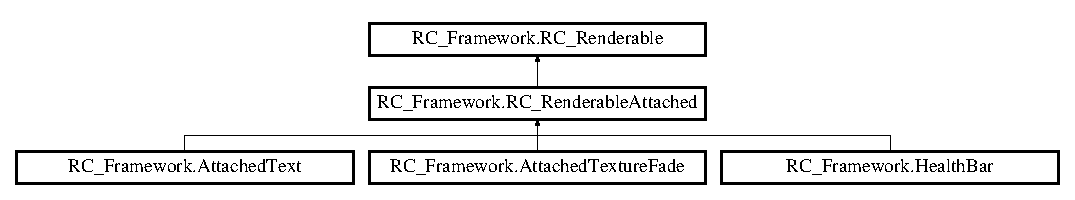
\includegraphics[height=2.240000cm]{class_r_c___framework_1_1_r_c___renderable_attached}
\end{center}
\end{figure}
\subsection*{Public Member Functions}
\begin{DoxyCompactItemize}
\item 
void \mbox{\hyperlink{class_r_c___framework_1_1_r_c___renderable_attached_aa8a7fd45e198635a8ee01c16877cfe8f}{set\+Parent}} (\mbox{\hyperlink{class_r_c___framework_1_1_sprite3}{Sprite3}} parentZ)
\end{DoxyCompactItemize}
\subsection*{Additional Inherited Members}


\subsection{Detailed Description}
A parent class for renderables attached to sprites that can be drawn after the sprite it lives off of the sprites update and draw sequences usefull for health bars and things 



\subsection{Member Function Documentation}
\mbox{\Hypertarget{class_r_c___framework_1_1_r_c___renderable_attached_aa8a7fd45e198635a8ee01c16877cfe8f}\label{class_r_c___framework_1_1_r_c___renderable_attached_aa8a7fd45e198635a8ee01c16877cfe8f}} 
\index{R\+C\+\_\+\+Framework\+::\+R\+C\+\_\+\+Renderable\+Attached@{R\+C\+\_\+\+Framework\+::\+R\+C\+\_\+\+Renderable\+Attached}!set\+Parent@{set\+Parent}}
\index{set\+Parent@{set\+Parent}!R\+C\+\_\+\+Framework\+::\+R\+C\+\_\+\+Renderable\+Attached@{R\+C\+\_\+\+Framework\+::\+R\+C\+\_\+\+Renderable\+Attached}}
\subsubsection{\texorpdfstring{set\+Parent()}{setParent()}}
{\footnotesize\ttfamily void R\+C\+\_\+\+Framework.\+R\+C\+\_\+\+Renderable\+Attached.\+set\+Parent (\begin{DoxyParamCaption}\item[{\mbox{\hyperlink{class_r_c___framework_1_1_sprite3}{Sprite3}}}]{parentZ }\end{DoxyParamCaption})}



The documentation for this class was generated from the following file\+:\begin{DoxyCompactItemize}
\item 
F\+:/\+B/\+R\+C\+\_\+\+Framework2018/\+Source/\mbox{\hyperlink{_r_c___renderable_parents_8cs}{R\+C\+\_\+\+Renderable\+Parents.\+cs}}\end{DoxyCompactItemize}

\hypertarget{class_r_c___framework_1_1_r_c___renderable_bounded}{}\section{R\+C\+\_\+\+Framework.\+R\+C\+\_\+\+Renderable\+Bounded Class Reference}
\label{class_r_c___framework_1_1_r_c___renderable_bounded}\index{R\+C\+\_\+\+Framework.\+R\+C\+\_\+\+Renderable\+Bounded@{R\+C\+\_\+\+Framework.\+R\+C\+\_\+\+Renderable\+Bounded}}


This class is a parent for a range of renderable class\textquotesingle{}s with a rectangle for bounds it allows seting the bounds by routines that resize it for zooming ~\newline
the bounds are definitly the render bounds not a collision box (though of course they may be the same)  


Inheritance diagram for R\+C\+\_\+\+Framework.\+R\+C\+\_\+\+Renderable\+Bounded\+:\begin{figure}[H]
\begin{center}
\leavevmode
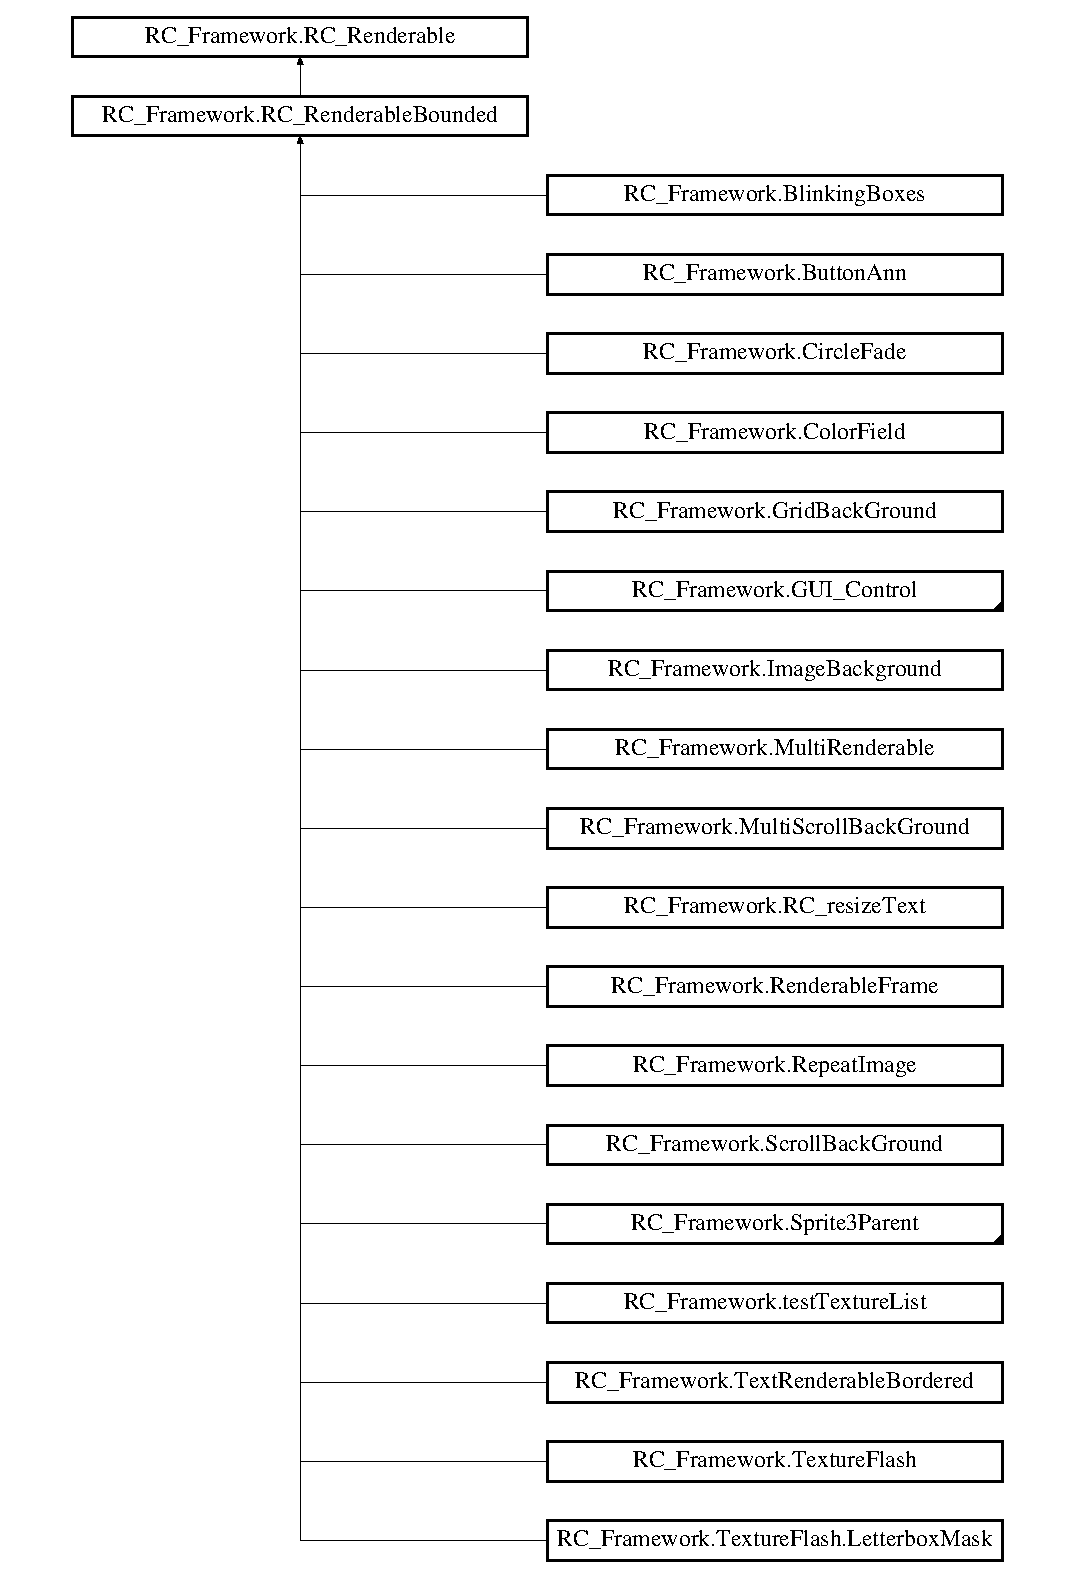
\includegraphics[height=12.000000cm]{class_r_c___framework_1_1_r_c___renderable_bounded}
\end{center}
\end{figure}
\subsection*{Public Member Functions}
\begin{DoxyCompactItemize}
\item 
virtual void \mbox{\hyperlink{class_r_c___framework_1_1_r_c___renderable_bounded_a49d38185d66bf150677aaf9cc35eb4fa}{set\+Pos}} (float x, float y)
\begin{DoxyCompactList}\small\item\em Set the x and y position of this renderable \end{DoxyCompactList}\item 
override bool \mbox{\hyperlink{class_r_c___framework_1_1_r_c___renderable_bounded_a000dd516577e50fb39fc3e1acc774435}{scroll\+Move}} (float x, float y)
\begin{DoxyCompactList}\small\item\em Used to scroll the entire screen -\/ while preserving old position usually called in renderable List Will have problemes with non integral scroll amounts (ie fractions) \end{DoxyCompactList}\item 
void \mbox{\hyperlink{class_r_c___framework_1_1_r_c___renderable_bounded_a871ee20b647861fb3fb93e112375db21}{set\+Width\+Height}} (int w, int h)
\begin{DoxyCompactList}\small\item\em set the width and height \end{DoxyCompactList}\item 
bool \mbox{\hyperlink{class_r_c___framework_1_1_r_c___renderable_bounded_a36f45a8174f4cee93a65085e015a2b2e}{Contains}} (int x, int y)
\begin{DoxyCompactList}\small\item\em Returns true if the renderable contains the point x,y \end{DoxyCompactList}\item 
Rectangle \mbox{\hyperlink{class_r_c___framework_1_1_r_c___renderable_bounded_a744532d85e586e0aa52f75dd1af3f60f}{Intersect}} (Rectangle r)
\begin{DoxyCompactList}\small\item\em Returns a rectangle which is the intersection of this renderable with another rectangle \end{DoxyCompactList}\item 
bool \mbox{\hyperlink{class_r_c___framework_1_1_r_c___renderable_bounded_a394581a8ad6bf9a472214fe4316ea37c}{Intersects}} (Rectangle r)
\begin{DoxyCompactList}\small\item\em Returns true if the rectange intersects this this renderable \end{DoxyCompactList}\item 
Vector2 \mbox{\hyperlink{class_r_c___framework_1_1_r_c___renderable_bounded_a93bf68209b9cf3bce7cbbd8eb02d6e1a}{get\+Sub\+Location}} (int sub\+Loc\+Num)
\begin{DoxyCompactList}\small\item\em Returns Various points in the rectangle \end{DoxyCompactList}\item 
bool \mbox{\hyperlink{class_r_c___framework_1_1_r_c___renderable_bounded_a126c01971f9ab5ac288b84aa985117e1}{inside}} (Rectangle r)
\begin{DoxyCompactList}\small\item\em Returns true if inside or on boundary of r \end{DoxyCompactList}\end{DoxyCompactItemize}
\subsection*{Protected Attributes}
\begin{DoxyCompactItemize}
\item 
Rectangle \mbox{\hyperlink{class_r_c___framework_1_1_r_c___renderable_bounded_aabcb0f8cd56a2e7b6209f8530194aff1}{boundz}}
\end{DoxyCompactItemize}
\subsection*{Properties}
\begin{DoxyCompactItemize}
\item 
virtual Rectangle \mbox{\hyperlink{class_r_c___framework_1_1_r_c___renderable_bounded_a64a3cd64146d7e7bc5897e5a849f158f}{bounds}}\hspace{0.3cm}{\ttfamily  \mbox{[}get, set\mbox{]}}
\end{DoxyCompactItemize}
\subsection*{Additional Inherited Members}


\subsection{Detailed Description}
This class is a parent for a range of renderable class\textquotesingle{}s with a rectangle for bounds it allows seting the bounds by routines that resize it for zooming ~\newline
the bounds are definitly the render bounds not a collision box (though of course they may be the same) 



\subsection{Member Function Documentation}
\mbox{\Hypertarget{class_r_c___framework_1_1_r_c___renderable_bounded_a36f45a8174f4cee93a65085e015a2b2e}\label{class_r_c___framework_1_1_r_c___renderable_bounded_a36f45a8174f4cee93a65085e015a2b2e}} 
\index{R\+C\+\_\+\+Framework\+::\+R\+C\+\_\+\+Renderable\+Bounded@{R\+C\+\_\+\+Framework\+::\+R\+C\+\_\+\+Renderable\+Bounded}!Contains@{Contains}}
\index{Contains@{Contains}!R\+C\+\_\+\+Framework\+::\+R\+C\+\_\+\+Renderable\+Bounded@{R\+C\+\_\+\+Framework\+::\+R\+C\+\_\+\+Renderable\+Bounded}}
\subsubsection{\texorpdfstring{Contains()}{Contains()}}
{\footnotesize\ttfamily bool R\+C\+\_\+\+Framework.\+R\+C\+\_\+\+Renderable\+Bounded.\+Contains (\begin{DoxyParamCaption}\item[{int}]{x,  }\item[{int}]{y }\end{DoxyParamCaption})}



Returns true if the renderable contains the point x,y 


\begin{DoxyParams}{Parameters}
{\em x} & \\
\hline
{\em y} & \\
\hline
\end{DoxyParams}
\begin{DoxyReturn}{Returns}

\end{DoxyReturn}
\mbox{\Hypertarget{class_r_c___framework_1_1_r_c___renderable_bounded_a93bf68209b9cf3bce7cbbd8eb02d6e1a}\label{class_r_c___framework_1_1_r_c___renderable_bounded_a93bf68209b9cf3bce7cbbd8eb02d6e1a}} 
\index{R\+C\+\_\+\+Framework\+::\+R\+C\+\_\+\+Renderable\+Bounded@{R\+C\+\_\+\+Framework\+::\+R\+C\+\_\+\+Renderable\+Bounded}!get\+Sub\+Location@{get\+Sub\+Location}}
\index{get\+Sub\+Location@{get\+Sub\+Location}!R\+C\+\_\+\+Framework\+::\+R\+C\+\_\+\+Renderable\+Bounded@{R\+C\+\_\+\+Framework\+::\+R\+C\+\_\+\+Renderable\+Bounded}}
\subsubsection{\texorpdfstring{get\+Sub\+Location()}{getSubLocation()}}
{\footnotesize\ttfamily Vector2 R\+C\+\_\+\+Framework.\+R\+C\+\_\+\+Renderable\+Bounded.\+get\+Sub\+Location (\begin{DoxyParamCaption}\item[{int}]{sub\+Loc\+Num }\end{DoxyParamCaption})}



Returns Various points in the rectangle 


\begin{DoxyParams}{Parameters}
{\em sub\+Loc\+Num} & \\
\hline
\end{DoxyParams}
\begin{DoxyReturn}{Returns}

\end{DoxyReturn}
\mbox{\Hypertarget{class_r_c___framework_1_1_r_c___renderable_bounded_a126c01971f9ab5ac288b84aa985117e1}\label{class_r_c___framework_1_1_r_c___renderable_bounded_a126c01971f9ab5ac288b84aa985117e1}} 
\index{R\+C\+\_\+\+Framework\+::\+R\+C\+\_\+\+Renderable\+Bounded@{R\+C\+\_\+\+Framework\+::\+R\+C\+\_\+\+Renderable\+Bounded}!inside@{inside}}
\index{inside@{inside}!R\+C\+\_\+\+Framework\+::\+R\+C\+\_\+\+Renderable\+Bounded@{R\+C\+\_\+\+Framework\+::\+R\+C\+\_\+\+Renderable\+Bounded}}
\subsubsection{\texorpdfstring{inside()}{inside()}}
{\footnotesize\ttfamily bool R\+C\+\_\+\+Framework.\+R\+C\+\_\+\+Renderable\+Bounded.\+inside (\begin{DoxyParamCaption}\item[{Rectangle}]{r }\end{DoxyParamCaption})}



Returns true if inside or on boundary of r 


\begin{DoxyParams}{Parameters}
{\em r} & \\
\hline
\end{DoxyParams}
\begin{DoxyReturn}{Returns}

\end{DoxyReturn}
\mbox{\Hypertarget{class_r_c___framework_1_1_r_c___renderable_bounded_a744532d85e586e0aa52f75dd1af3f60f}\label{class_r_c___framework_1_1_r_c___renderable_bounded_a744532d85e586e0aa52f75dd1af3f60f}} 
\index{R\+C\+\_\+\+Framework\+::\+R\+C\+\_\+\+Renderable\+Bounded@{R\+C\+\_\+\+Framework\+::\+R\+C\+\_\+\+Renderable\+Bounded}!Intersect@{Intersect}}
\index{Intersect@{Intersect}!R\+C\+\_\+\+Framework\+::\+R\+C\+\_\+\+Renderable\+Bounded@{R\+C\+\_\+\+Framework\+::\+R\+C\+\_\+\+Renderable\+Bounded}}
\subsubsection{\texorpdfstring{Intersect()}{Intersect()}}
{\footnotesize\ttfamily Rectangle R\+C\+\_\+\+Framework.\+R\+C\+\_\+\+Renderable\+Bounded.\+Intersect (\begin{DoxyParamCaption}\item[{Rectangle}]{r }\end{DoxyParamCaption})}



Returns a rectangle which is the intersection of this renderable with another rectangle 


\begin{DoxyParams}{Parameters}
{\em r} & \\
\hline
\end{DoxyParams}
\begin{DoxyReturn}{Returns}

\end{DoxyReturn}
\mbox{\Hypertarget{class_r_c___framework_1_1_r_c___renderable_bounded_a394581a8ad6bf9a472214fe4316ea37c}\label{class_r_c___framework_1_1_r_c___renderable_bounded_a394581a8ad6bf9a472214fe4316ea37c}} 
\index{R\+C\+\_\+\+Framework\+::\+R\+C\+\_\+\+Renderable\+Bounded@{R\+C\+\_\+\+Framework\+::\+R\+C\+\_\+\+Renderable\+Bounded}!Intersects@{Intersects}}
\index{Intersects@{Intersects}!R\+C\+\_\+\+Framework\+::\+R\+C\+\_\+\+Renderable\+Bounded@{R\+C\+\_\+\+Framework\+::\+R\+C\+\_\+\+Renderable\+Bounded}}
\subsubsection{\texorpdfstring{Intersects()}{Intersects()}}
{\footnotesize\ttfamily bool R\+C\+\_\+\+Framework.\+R\+C\+\_\+\+Renderable\+Bounded.\+Intersects (\begin{DoxyParamCaption}\item[{Rectangle}]{r }\end{DoxyParamCaption})}



Returns true if the rectange intersects this this renderable 


\begin{DoxyParams}{Parameters}
{\em r} & \\
\hline
\end{DoxyParams}
\begin{DoxyReturn}{Returns}

\end{DoxyReturn}
\mbox{\Hypertarget{class_r_c___framework_1_1_r_c___renderable_bounded_a000dd516577e50fb39fc3e1acc774435}\label{class_r_c___framework_1_1_r_c___renderable_bounded_a000dd516577e50fb39fc3e1acc774435}} 
\index{R\+C\+\_\+\+Framework\+::\+R\+C\+\_\+\+Renderable\+Bounded@{R\+C\+\_\+\+Framework\+::\+R\+C\+\_\+\+Renderable\+Bounded}!scroll\+Move@{scroll\+Move}}
\index{scroll\+Move@{scroll\+Move}!R\+C\+\_\+\+Framework\+::\+R\+C\+\_\+\+Renderable\+Bounded@{R\+C\+\_\+\+Framework\+::\+R\+C\+\_\+\+Renderable\+Bounded}}
\subsubsection{\texorpdfstring{scroll\+Move()}{scrollMove()}}
{\footnotesize\ttfamily override bool R\+C\+\_\+\+Framework.\+R\+C\+\_\+\+Renderable\+Bounded.\+scroll\+Move (\begin{DoxyParamCaption}\item[{float}]{x,  }\item[{float}]{y }\end{DoxyParamCaption})\hspace{0.3cm}{\ttfamily [virtual]}}



Used to scroll the entire screen -\/ while preserving old position usually called in renderable List Will have problemes with non integral scroll amounts (ie fractions) 


\begin{DoxyParams}{Parameters}
{\em x} & the amount to scroll in x \\
\hline
{\em y} & the amount to scroll in y\\
\hline
\end{DoxyParams}
\begin{DoxyReturn}{Returns}
true if successfull 
\end{DoxyReturn}


Reimplemented from \mbox{\hyperlink{class_r_c___framework_1_1_r_c___renderable_a21e5b1a68c7382443c82e7296fd2209a}{R\+C\+\_\+\+Framework.\+R\+C\+\_\+\+Renderable}}.



Reimplemented in \mbox{\hyperlink{class_r_c___framework_1_1_sprite3_ab4c64556d7bcebf5ce538631ae9b5d6c}{R\+C\+\_\+\+Framework.\+Sprite3}}.

\mbox{\Hypertarget{class_r_c___framework_1_1_r_c___renderable_bounded_a49d38185d66bf150677aaf9cc35eb4fa}\label{class_r_c___framework_1_1_r_c___renderable_bounded_a49d38185d66bf150677aaf9cc35eb4fa}} 
\index{R\+C\+\_\+\+Framework\+::\+R\+C\+\_\+\+Renderable\+Bounded@{R\+C\+\_\+\+Framework\+::\+R\+C\+\_\+\+Renderable\+Bounded}!set\+Pos@{set\+Pos}}
\index{set\+Pos@{set\+Pos}!R\+C\+\_\+\+Framework\+::\+R\+C\+\_\+\+Renderable\+Bounded@{R\+C\+\_\+\+Framework\+::\+R\+C\+\_\+\+Renderable\+Bounded}}
\subsubsection{\texorpdfstring{set\+Pos()}{setPos()}}
{\footnotesize\ttfamily virtual void R\+C\+\_\+\+Framework.\+R\+C\+\_\+\+Renderable\+Bounded.\+set\+Pos (\begin{DoxyParamCaption}\item[{float}]{x,  }\item[{float}]{y }\end{DoxyParamCaption})\hspace{0.3cm}{\ttfamily [virtual]}}



Set the x and y position of this renderable 


\begin{DoxyParams}{Parameters}
{\em x} & \\
\hline
{\em y} & \\
\hline
\end{DoxyParams}


Reimplemented in \mbox{\hyperlink{class_r_c___framework_1_1_sprite3_parent_aafe2f4e919b30044d02600942068d205}{R\+C\+\_\+\+Framework.\+Sprite3\+Parent}}.

\mbox{\Hypertarget{class_r_c___framework_1_1_r_c___renderable_bounded_a871ee20b647861fb3fb93e112375db21}\label{class_r_c___framework_1_1_r_c___renderable_bounded_a871ee20b647861fb3fb93e112375db21}} 
\index{R\+C\+\_\+\+Framework\+::\+R\+C\+\_\+\+Renderable\+Bounded@{R\+C\+\_\+\+Framework\+::\+R\+C\+\_\+\+Renderable\+Bounded}!set\+Width\+Height@{set\+Width\+Height}}
\index{set\+Width\+Height@{set\+Width\+Height}!R\+C\+\_\+\+Framework\+::\+R\+C\+\_\+\+Renderable\+Bounded@{R\+C\+\_\+\+Framework\+::\+R\+C\+\_\+\+Renderable\+Bounded}}
\subsubsection{\texorpdfstring{set\+Width\+Height()}{setWidthHeight()}}
{\footnotesize\ttfamily void R\+C\+\_\+\+Framework.\+R\+C\+\_\+\+Renderable\+Bounded.\+set\+Width\+Height (\begin{DoxyParamCaption}\item[{int}]{w,  }\item[{int}]{h }\end{DoxyParamCaption})}



set the width and height 


\begin{DoxyParams}{Parameters}
{\em w} & \\
\hline
{\em h} & \\
\hline
\end{DoxyParams}


\subsection{Member Data Documentation}
\mbox{\Hypertarget{class_r_c___framework_1_1_r_c___renderable_bounded_aabcb0f8cd56a2e7b6209f8530194aff1}\label{class_r_c___framework_1_1_r_c___renderable_bounded_aabcb0f8cd56a2e7b6209f8530194aff1}} 
\index{R\+C\+\_\+\+Framework\+::\+R\+C\+\_\+\+Renderable\+Bounded@{R\+C\+\_\+\+Framework\+::\+R\+C\+\_\+\+Renderable\+Bounded}!boundz@{boundz}}
\index{boundz@{boundz}!R\+C\+\_\+\+Framework\+::\+R\+C\+\_\+\+Renderable\+Bounded@{R\+C\+\_\+\+Framework\+::\+R\+C\+\_\+\+Renderable\+Bounded}}
\subsubsection{\texorpdfstring{boundz}{boundz}}
{\footnotesize\ttfamily Rectangle R\+C\+\_\+\+Framework.\+R\+C\+\_\+\+Renderable\+Bounded.\+boundz\hspace{0.3cm}{\ttfamily [protected]}}



\subsection{Property Documentation}
\mbox{\Hypertarget{class_r_c___framework_1_1_r_c___renderable_bounded_a64a3cd64146d7e7bc5897e5a849f158f}\label{class_r_c___framework_1_1_r_c___renderable_bounded_a64a3cd64146d7e7bc5897e5a849f158f}} 
\index{R\+C\+\_\+\+Framework\+::\+R\+C\+\_\+\+Renderable\+Bounded@{R\+C\+\_\+\+Framework\+::\+R\+C\+\_\+\+Renderable\+Bounded}!bounds@{bounds}}
\index{bounds@{bounds}!R\+C\+\_\+\+Framework\+::\+R\+C\+\_\+\+Renderable\+Bounded@{R\+C\+\_\+\+Framework\+::\+R\+C\+\_\+\+Renderable\+Bounded}}
\subsubsection{\texorpdfstring{bounds}{bounds}}
{\footnotesize\ttfamily virtual Rectangle R\+C\+\_\+\+Framework.\+R\+C\+\_\+\+Renderable\+Bounded.\+bounds\hspace{0.3cm}{\ttfamily [get]}, {\ttfamily [set]}}



The documentation for this class was generated from the following file\+:\begin{DoxyCompactItemize}
\item 
F\+:/\+B/\+R\+C\+\_\+\+Framework2018/\+Source/\mbox{\hyperlink{_r_c___renderable_parents_8cs}{R\+C\+\_\+\+Renderable\+Parents.\+cs}}\end{DoxyCompactItemize}

\hypertarget{class_r_c___framework_1_1_r_c___renderable_list}{}\section{R\+C\+\_\+\+Framework.\+R\+C\+\_\+\+Renderable\+List Class Reference}
\label{class_r_c___framework_1_1_r_c___renderable_list}\index{R\+C\+\_\+\+Framework.\+R\+C\+\_\+\+Renderable\+List@{R\+C\+\_\+\+Framework.\+R\+C\+\_\+\+Renderable\+List}}


a list of renderables the idea of the active flag is is that inactive renderables can have their place re-\/used and are no longer needed  


Inheritance diagram for R\+C\+\_\+\+Framework.\+R\+C\+\_\+\+Renderable\+List\+:\begin{figure}[H]
\begin{center}
\leavevmode
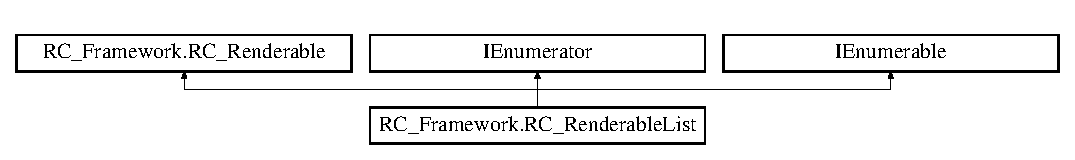
\includegraphics[height=1.704718cm]{class_r_c___framework_1_1_r_c___renderable_list}
\end{center}
\end{figure}
\subsection*{Public Member Functions}
\begin{DoxyCompactItemize}
\item 
\mbox{\hyperlink{class_r_c___framework_1_1_r_c___renderable_list_a9fa56c1b694187351daa9b464722ec1b}{R\+C\+\_\+\+Renderable\+List}} ()
\item 
bool \mbox{\hyperlink{class_r_c___framework_1_1_r_c___renderable_list_a2974cbded928cdb237fadf5c8adbdd2c}{Move\+Next}} ()
\item 
void \mbox{\hyperlink{class_r_c___framework_1_1_r_c___renderable_list_ac70aff9f6f35ecb69378a70ad8e41f0e}{Reset}} ()
\item 
void \mbox{\hyperlink{class_r_c___framework_1_1_r_c___renderable_list_aaae1bbc19f649e2930c8c829625c9a5e}{Dispose}} ()
\item 
I\+Enumerator \mbox{\hyperlink{class_r_c___framework_1_1_r_c___renderable_list_a0c8e476d6928961b5e6e4e4a3d37bba9}{Get\+Enumerator}} ()
\item 
override void \mbox{\hyperlink{class_r_c___framework_1_1_r_c___renderable_list_a274ae54ac48b42415db6b3193587e8d4}{Draw}} (Sprite\+Batch sb)
\begin{DoxyCompactList}\small\item\em draw the list of renderables renderables are responsible for knowing their position \end{DoxyCompactList}\item 
override void \mbox{\hyperlink{class_r_c___framework_1_1_r_c___renderable_list_a2de302d2ee2f4df7c90fb7df36c4f3fe}{Update}} (Game\+Time game\+Time)
\begin{DoxyCompactList}\small\item\em run update on the entire list of renderables \end{DoxyCompactList}\item 
override bool \mbox{\hyperlink{class_r_c___framework_1_1_r_c___renderable_list_ad7238f93a7ad63020771702a2db0ccfe}{scroll\+Move}} (float x, float y)
\begin{DoxyCompactList}\small\item\em runs scroll move on all renderables used to scroll the screen \end{DoxyCompactList}\item 
override void \mbox{\hyperlink{class_r_c___framework_1_1_r_c___renderable_list_a953e8eb6f4422a7f0bebb17ee0455c42}{Load\+Content}} ()
\begin{DoxyCompactList}\small\item\em For initialisation \end{DoxyCompactList}\item 
int \mbox{\hyperlink{class_r_c___framework_1_1_r_c___renderable_list_acc544e521274aaf092219cd33b59cf86}{Index\+Of}} (\mbox{\hyperlink{class_r_c___framework_1_1_r_c___renderable}{R\+C\+\_\+\+Renderable}} item)
\begin{DoxyCompactList}\small\item\em This returns the index of a given renderable \end{DoxyCompactList}\item 
int \mbox{\hyperlink{class_r_c___framework_1_1_r_c___renderable_list_aa18cdc63b500d558e79c9a73ae668b30}{Index\+Of\+Previous}} (\mbox{\hyperlink{class_r_c___framework_1_1_r_c___renderable}{R\+C\+\_\+\+Renderable}} item)
\begin{DoxyCompactList}\small\item\em This returns the index of the previous renderable in most cases it makes no senseits probably only usefull in gui applications it assumes the renderables are placed in the list an a meaningfull order \end{DoxyCompactList}\item 
int \mbox{\hyperlink{class_r_c___framework_1_1_r_c___renderable_list_a8871117c0fd0d66d14f3b3049e3c7712}{Index\+Of\+Next}} (\mbox{\hyperlink{class_r_c___framework_1_1_r_c___renderable}{R\+C\+\_\+\+Renderable}} item)
\begin{DoxyCompactList}\small\item\em This returns the index of the next renderable in most cases it makes no senseits probably only usefull in gui applications it assumes the renderables are placed in the list an a meaningfull order \end{DoxyCompactList}\item 
void \mbox{\hyperlink{class_r_c___framework_1_1_r_c___renderable_list_aa03dda23b963f5392732f0ee59cfc388}{add\+Reuse}} (\mbox{\hyperlink{class_r_c___framework_1_1_r_c___renderable}{R\+C\+\_\+\+Renderable}} r)
\begin{DoxyCompactList}\small\item\em standard way to add things to the list reusing old space to stop the list growing to long \end{DoxyCompactList}\item 
void \mbox{\hyperlink{class_r_c___framework_1_1_r_c___renderable_list_a9b760ae083aa63818a0789ba10d0af40}{add\+To\+End}} (\mbox{\hyperlink{class_r_c___framework_1_1_r_c___renderable}{R\+C\+\_\+\+Renderable}} r)
\begin{DoxyCompactList}\small\item\em Adds to the list -\/ fast but usually we would use the \textquotesingle{}add\+Reuse\textquotesingle{} method \end{DoxyCompactList}\item 
int \mbox{\hyperlink{class_r_c___framework_1_1_r_c___renderable_list_aefabaf7b1a4e5e163d4a6e77cc07b94a}{find\+Inactive}} ()
\begin{DoxyCompactList}\small\item\em internal use mainly \end{DoxyCompactList}\item 
\mbox{\hyperlink{class_r_c___framework_1_1_r_c___renderable}{R\+C\+\_\+\+Renderable}} \mbox{\hyperlink{class_r_c___framework_1_1_r_c___renderable_list_abb4dfff8d5e8ac2e96034e591c96d811}{replace}} (int num, \mbox{\hyperlink{class_r_c___framework_1_1_r_c___renderable}{R\+C\+\_\+\+Renderable}} r)
\begin{DoxyCompactList}\small\item\em replaces returning the old value -\/ not especially usefull \end{DoxyCompactList}\item 
\mbox{\hyperlink{class_r_c___framework_1_1_r_c___renderable}{R\+C\+\_\+\+Renderable}} \mbox{\hyperlink{class_r_c___framework_1_1_r_c___renderable_list_a75b4ae92f064d35358185fe12bda892c}{get\+Renderable}} (int i)
\begin{DoxyCompactList}\small\item\em gets a renderable i \end{DoxyCompactList}\item 
int \mbox{\hyperlink{class_r_c___framework_1_1_r_c___renderable_list_a89f525ac211787c14d1b16f925bc4558}{Count}} ()
\begin{DoxyCompactList}\small\item\em Count of renderable \end{DoxyCompactList}\item 
int \mbox{\hyperlink{class_r_c___framework_1_1_r_c___renderable_list_afab33aa056d75a88414f62576aa0cbd9}{Contains}} (float x, float y)
\begin{DoxyCompactList}\small\item\em If the renderable list contains \mbox{\hyperlink{class_r_c___framework_1_1_r_c___renderable_bounded}{R\+C\+\_\+\+Renderable\+Bounded}} it will return the first renderable index that this point in bounds or -\/1 if not found \end{DoxyCompactList}\item 
int \mbox{\hyperlink{class_r_c___framework_1_1_r_c___renderable_list_aa38871296e0b22f5c1c80ba82605f0ba}{collision}} (Rectangle r)
\begin{DoxyCompactList}\small\item\em Checks for collision with rectangle for bounded renderables only \end{DoxyCompactList}\item 
override void \mbox{\hyperlink{class_r_c___framework_1_1_r_c___renderable_list_a8cba0458aba6bbf1b4d7b57217060f43}{set\+Color}} (Color c)
\begin{DoxyCompactList}\small\item\em Sets colour for all active renderables \end{DoxyCompactList}\item 
int \mbox{\hyperlink{class_r_c___framework_1_1_r_c___renderable_list_a343637f6337ee79256fcba579e2a69be}{count\+Of\+Active}} ()
\begin{DoxyCompactList}\small\item\em Counts the active renderables deprecated please use count\+Active \end{DoxyCompactList}\item 
override bool \mbox{\hyperlink{class_r_c___framework_1_1_r_c___renderable_list_a5867cf3044d40adda1bb7c2be3211a99}{Mouse\+Over}} (float mouse\+\_\+x, float mouse\+\_\+y)
\item 
override bool \mbox{\hyperlink{class_r_c___framework_1_1_r_c___renderable_list_adce00726f7093db725ed6195292156a7}{Mouse\+Down\+Event\+Left}} (float mouse\+\_\+x, float mouse\+\_\+y)
\begin{DoxyCompactList}\small\item\em Propagates a mouse down on left button till consumed \end{DoxyCompactList}\item 
override bool \mbox{\hyperlink{class_r_c___framework_1_1_r_c___renderable_list_ac275d3df45899b62e1378e01a100268d}{Mouse\+Click\+Event}} (float mouse\+\_\+x, float mouse\+\_\+y)
\begin{DoxyCompactList}\small\item\em Propagates a mouse click till consumed \end{DoxyCompactList}\item 
override bool \mbox{\hyperlink{class_r_c___framework_1_1_r_c___renderable_list_a221a0bf056ff4f8e02d22e3b8b66de81}{Key\+Hit\+Event}} (Keys key\+Hit)
\begin{DoxyCompactList}\small\item\em propagates a keyhit event till its consumed \end{DoxyCompactList}\item 
int \mbox{\hyperlink{class_r_c___framework_1_1_r_c___renderable_list_a5743c82009f4d250d03bdbf1ee32bdcc}{count\+Active}} ()
\begin{DoxyCompactList}\small\item\em count of active renderable \end{DoxyCompactList}\item 
bool \mbox{\hyperlink{class_r_c___framework_1_1_r_c___renderable_list_a65b0bbae9d1d83579d269d756a3626e3}{Run\+The\+Method}} (Func$<$ \mbox{\hyperlink{class_r_c___framework_1_1_r_c___renderable}{R\+C\+\_\+\+Renderable}}, bool $>$ method\+Name)
\begin{DoxyCompactList}\small\item\em Run the method on each active renderables return true only if all functions return true or there are no active renderables the function has the formal parameters bool name(\+R\+C\+\_\+\+Renderable s) \end{DoxyCompactList}\end{DoxyCompactItemize}
\subsection*{Public Attributes}
\begin{DoxyCompactItemize}
\item 
List$<$ \mbox{\hyperlink{class_r_c___framework_1_1_r_c___renderable}{R\+C\+\_\+\+Renderable}} $>$ \mbox{\hyperlink{class_r_c___framework_1_1_r_c___renderable_list_ab54b7af85213b25a5d66cd169c27b352}{rlist}}
\end{DoxyCompactItemize}
\subsection*{Properties}
\begin{DoxyCompactItemize}
\item 
\mbox{\hyperlink{class_r_c___framework_1_1_r_c___renderable}{R\+C\+\_\+\+Renderable}} \mbox{\hyperlink{class_r_c___framework_1_1_r_c___renderable_list_a8a63966970b03403ce48e9bcca4f795d}{this\mbox{[}int key\mbox{]}}}\hspace{0.3cm}{\ttfamily  \mbox{[}get, set\mbox{]}}
\begin{DoxyCompactList}\small\item\em Overload \mbox{[} and \mbox{]} for ease of use \end{DoxyCompactList}\item 
object \mbox{\hyperlink{class_r_c___framework_1_1_r_c___renderable_list_ad9d22dbadf2d32491b2bfad15acb37dd}{Current}}\hspace{0.3cm}{\ttfamily  \mbox{[}get\mbox{]}}
\end{DoxyCompactItemize}


\subsection{Detailed Description}
a list of renderables the idea of the active flag is is that inactive renderables can have their place re-\/used and are no longer needed 



\subsection{Constructor \& Destructor Documentation}
\mbox{\Hypertarget{class_r_c___framework_1_1_r_c___renderable_list_a9fa56c1b694187351daa9b464722ec1b}\label{class_r_c___framework_1_1_r_c___renderable_list_a9fa56c1b694187351daa9b464722ec1b}} 
\index{R\+C\+\_\+\+Framework\+::\+R\+C\+\_\+\+Renderable\+List@{R\+C\+\_\+\+Framework\+::\+R\+C\+\_\+\+Renderable\+List}!R\+C\+\_\+\+Renderable\+List@{R\+C\+\_\+\+Renderable\+List}}
\index{R\+C\+\_\+\+Renderable\+List@{R\+C\+\_\+\+Renderable\+List}!R\+C\+\_\+\+Framework\+::\+R\+C\+\_\+\+Renderable\+List@{R\+C\+\_\+\+Framework\+::\+R\+C\+\_\+\+Renderable\+List}}
\subsubsection{\texorpdfstring{R\+C\+\_\+\+Renderable\+List()}{RC\_RenderableList()}}
{\footnotesize\ttfamily R\+C\+\_\+\+Framework.\+R\+C\+\_\+\+Renderable\+List.\+R\+C\+\_\+\+Renderable\+List (\begin{DoxyParamCaption}{ }\end{DoxyParamCaption})}



\subsection{Member Function Documentation}
\mbox{\Hypertarget{class_r_c___framework_1_1_r_c___renderable_list_aa03dda23b963f5392732f0ee59cfc388}\label{class_r_c___framework_1_1_r_c___renderable_list_aa03dda23b963f5392732f0ee59cfc388}} 
\index{R\+C\+\_\+\+Framework\+::\+R\+C\+\_\+\+Renderable\+List@{R\+C\+\_\+\+Framework\+::\+R\+C\+\_\+\+Renderable\+List}!add\+Reuse@{add\+Reuse}}
\index{add\+Reuse@{add\+Reuse}!R\+C\+\_\+\+Framework\+::\+R\+C\+\_\+\+Renderable\+List@{R\+C\+\_\+\+Framework\+::\+R\+C\+\_\+\+Renderable\+List}}
\subsubsection{\texorpdfstring{add\+Reuse()}{addReuse()}}
{\footnotesize\ttfamily void R\+C\+\_\+\+Framework.\+R\+C\+\_\+\+Renderable\+List.\+add\+Reuse (\begin{DoxyParamCaption}\item[{\mbox{\hyperlink{class_r_c___framework_1_1_r_c___renderable}{R\+C\+\_\+\+Renderable}}}]{r }\end{DoxyParamCaption})}



standard way to add things to the list reusing old space to stop the list growing to long 


\begin{DoxyParams}{Parameters}
{\em r} & \\
\hline
\end{DoxyParams}
\mbox{\Hypertarget{class_r_c___framework_1_1_r_c___renderable_list_a9b760ae083aa63818a0789ba10d0af40}\label{class_r_c___framework_1_1_r_c___renderable_list_a9b760ae083aa63818a0789ba10d0af40}} 
\index{R\+C\+\_\+\+Framework\+::\+R\+C\+\_\+\+Renderable\+List@{R\+C\+\_\+\+Framework\+::\+R\+C\+\_\+\+Renderable\+List}!add\+To\+End@{add\+To\+End}}
\index{add\+To\+End@{add\+To\+End}!R\+C\+\_\+\+Framework\+::\+R\+C\+\_\+\+Renderable\+List@{R\+C\+\_\+\+Framework\+::\+R\+C\+\_\+\+Renderable\+List}}
\subsubsection{\texorpdfstring{add\+To\+End()}{addToEnd()}}
{\footnotesize\ttfamily void R\+C\+\_\+\+Framework.\+R\+C\+\_\+\+Renderable\+List.\+add\+To\+End (\begin{DoxyParamCaption}\item[{\mbox{\hyperlink{class_r_c___framework_1_1_r_c___renderable}{R\+C\+\_\+\+Renderable}}}]{r }\end{DoxyParamCaption})}



Adds to the list -\/ fast but usually we would use the \textquotesingle{}add\+Reuse\textquotesingle{} method 


\begin{DoxyParams}{Parameters}
{\em r} & \\
\hline
\end{DoxyParams}
\mbox{\Hypertarget{class_r_c___framework_1_1_r_c___renderable_list_aa38871296e0b22f5c1c80ba82605f0ba}\label{class_r_c___framework_1_1_r_c___renderable_list_aa38871296e0b22f5c1c80ba82605f0ba}} 
\index{R\+C\+\_\+\+Framework\+::\+R\+C\+\_\+\+Renderable\+List@{R\+C\+\_\+\+Framework\+::\+R\+C\+\_\+\+Renderable\+List}!collision@{collision}}
\index{collision@{collision}!R\+C\+\_\+\+Framework\+::\+R\+C\+\_\+\+Renderable\+List@{R\+C\+\_\+\+Framework\+::\+R\+C\+\_\+\+Renderable\+List}}
\subsubsection{\texorpdfstring{collision()}{collision()}}
{\footnotesize\ttfamily int R\+C\+\_\+\+Framework.\+R\+C\+\_\+\+Renderable\+List.\+collision (\begin{DoxyParamCaption}\item[{Rectangle}]{r }\end{DoxyParamCaption})}



Checks for collision with rectangle for bounded renderables only 


\begin{DoxyParams}{Parameters}
{\em r} & \\
\hline
\end{DoxyParams}
\begin{DoxyReturn}{Returns}

\end{DoxyReturn}
\mbox{\Hypertarget{class_r_c___framework_1_1_r_c___renderable_list_afab33aa056d75a88414f62576aa0cbd9}\label{class_r_c___framework_1_1_r_c___renderable_list_afab33aa056d75a88414f62576aa0cbd9}} 
\index{R\+C\+\_\+\+Framework\+::\+R\+C\+\_\+\+Renderable\+List@{R\+C\+\_\+\+Framework\+::\+R\+C\+\_\+\+Renderable\+List}!Contains@{Contains}}
\index{Contains@{Contains}!R\+C\+\_\+\+Framework\+::\+R\+C\+\_\+\+Renderable\+List@{R\+C\+\_\+\+Framework\+::\+R\+C\+\_\+\+Renderable\+List}}
\subsubsection{\texorpdfstring{Contains()}{Contains()}}
{\footnotesize\ttfamily int R\+C\+\_\+\+Framework.\+R\+C\+\_\+\+Renderable\+List.\+Contains (\begin{DoxyParamCaption}\item[{float}]{x,  }\item[{float}]{y }\end{DoxyParamCaption})}



If the renderable list contains \mbox{\hyperlink{class_r_c___framework_1_1_r_c___renderable_bounded}{R\+C\+\_\+\+Renderable\+Bounded}} it will return the first renderable index that this point in bounds or -\/1 if not found 


\begin{DoxyParams}{Parameters}
{\em x} & \\
\hline
{\em y} & \\
\hline
\end{DoxyParams}
\begin{DoxyReturn}{Returns}

\end{DoxyReturn}
\mbox{\Hypertarget{class_r_c___framework_1_1_r_c___renderable_list_a89f525ac211787c14d1b16f925bc4558}\label{class_r_c___framework_1_1_r_c___renderable_list_a89f525ac211787c14d1b16f925bc4558}} 
\index{R\+C\+\_\+\+Framework\+::\+R\+C\+\_\+\+Renderable\+List@{R\+C\+\_\+\+Framework\+::\+R\+C\+\_\+\+Renderable\+List}!Count@{Count}}
\index{Count@{Count}!R\+C\+\_\+\+Framework\+::\+R\+C\+\_\+\+Renderable\+List@{R\+C\+\_\+\+Framework\+::\+R\+C\+\_\+\+Renderable\+List}}
\subsubsection{\texorpdfstring{Count()}{Count()}}
{\footnotesize\ttfamily int R\+C\+\_\+\+Framework.\+R\+C\+\_\+\+Renderable\+List.\+Count (\begin{DoxyParamCaption}{ }\end{DoxyParamCaption})}



Count of renderable 

\begin{DoxyReturn}{Returns}

\end{DoxyReturn}
\mbox{\Hypertarget{class_r_c___framework_1_1_r_c___renderable_list_a5743c82009f4d250d03bdbf1ee32bdcc}\label{class_r_c___framework_1_1_r_c___renderable_list_a5743c82009f4d250d03bdbf1ee32bdcc}} 
\index{R\+C\+\_\+\+Framework\+::\+R\+C\+\_\+\+Renderable\+List@{R\+C\+\_\+\+Framework\+::\+R\+C\+\_\+\+Renderable\+List}!count\+Active@{count\+Active}}
\index{count\+Active@{count\+Active}!R\+C\+\_\+\+Framework\+::\+R\+C\+\_\+\+Renderable\+List@{R\+C\+\_\+\+Framework\+::\+R\+C\+\_\+\+Renderable\+List}}
\subsubsection{\texorpdfstring{count\+Active()}{countActive()}}
{\footnotesize\ttfamily int R\+C\+\_\+\+Framework.\+R\+C\+\_\+\+Renderable\+List.\+count\+Active (\begin{DoxyParamCaption}{ }\end{DoxyParamCaption})}



count of active renderable 

\begin{DoxyReturn}{Returns}

\end{DoxyReturn}
\mbox{\Hypertarget{class_r_c___framework_1_1_r_c___renderable_list_a343637f6337ee79256fcba579e2a69be}\label{class_r_c___framework_1_1_r_c___renderable_list_a343637f6337ee79256fcba579e2a69be}} 
\index{R\+C\+\_\+\+Framework\+::\+R\+C\+\_\+\+Renderable\+List@{R\+C\+\_\+\+Framework\+::\+R\+C\+\_\+\+Renderable\+List}!count\+Of\+Active@{count\+Of\+Active}}
\index{count\+Of\+Active@{count\+Of\+Active}!R\+C\+\_\+\+Framework\+::\+R\+C\+\_\+\+Renderable\+List@{R\+C\+\_\+\+Framework\+::\+R\+C\+\_\+\+Renderable\+List}}
\subsubsection{\texorpdfstring{count\+Of\+Active()}{countOfActive()}}
{\footnotesize\ttfamily int R\+C\+\_\+\+Framework.\+R\+C\+\_\+\+Renderable\+List.\+count\+Of\+Active (\begin{DoxyParamCaption}{ }\end{DoxyParamCaption})}



Counts the active renderables deprecated please use count\+Active 

\begin{DoxyReturn}{Returns}

\end{DoxyReturn}
\mbox{\Hypertarget{class_r_c___framework_1_1_r_c___renderable_list_aaae1bbc19f649e2930c8c829625c9a5e}\label{class_r_c___framework_1_1_r_c___renderable_list_aaae1bbc19f649e2930c8c829625c9a5e}} 
\index{R\+C\+\_\+\+Framework\+::\+R\+C\+\_\+\+Renderable\+List@{R\+C\+\_\+\+Framework\+::\+R\+C\+\_\+\+Renderable\+List}!Dispose@{Dispose}}
\index{Dispose@{Dispose}!R\+C\+\_\+\+Framework\+::\+R\+C\+\_\+\+Renderable\+List@{R\+C\+\_\+\+Framework\+::\+R\+C\+\_\+\+Renderable\+List}}
\subsubsection{\texorpdfstring{Dispose()}{Dispose()}}
{\footnotesize\ttfamily void R\+C\+\_\+\+Framework.\+R\+C\+\_\+\+Renderable\+List.\+Dispose (\begin{DoxyParamCaption}{ }\end{DoxyParamCaption})}

\mbox{\Hypertarget{class_r_c___framework_1_1_r_c___renderable_list_a274ae54ac48b42415db6b3193587e8d4}\label{class_r_c___framework_1_1_r_c___renderable_list_a274ae54ac48b42415db6b3193587e8d4}} 
\index{R\+C\+\_\+\+Framework\+::\+R\+C\+\_\+\+Renderable\+List@{R\+C\+\_\+\+Framework\+::\+R\+C\+\_\+\+Renderable\+List}!Draw@{Draw}}
\index{Draw@{Draw}!R\+C\+\_\+\+Framework\+::\+R\+C\+\_\+\+Renderable\+List@{R\+C\+\_\+\+Framework\+::\+R\+C\+\_\+\+Renderable\+List}}
\subsubsection{\texorpdfstring{Draw()}{Draw()}}
{\footnotesize\ttfamily override void R\+C\+\_\+\+Framework.\+R\+C\+\_\+\+Renderable\+List.\+Draw (\begin{DoxyParamCaption}\item[{Sprite\+Batch}]{sb }\end{DoxyParamCaption})\hspace{0.3cm}{\ttfamily [virtual]}}



draw the list of renderables renderables are responsible for knowing their position 


\begin{DoxyParams}{Parameters}
{\em sb} & \\
\hline
\end{DoxyParams}


Reimplemented from \mbox{\hyperlink{class_r_c___framework_1_1_r_c___renderable_acc26db34e382a25a989c4c0dd0354b23}{R\+C\+\_\+\+Framework.\+R\+C\+\_\+\+Renderable}}.

\mbox{\Hypertarget{class_r_c___framework_1_1_r_c___renderable_list_aefabaf7b1a4e5e163d4a6e77cc07b94a}\label{class_r_c___framework_1_1_r_c___renderable_list_aefabaf7b1a4e5e163d4a6e77cc07b94a}} 
\index{R\+C\+\_\+\+Framework\+::\+R\+C\+\_\+\+Renderable\+List@{R\+C\+\_\+\+Framework\+::\+R\+C\+\_\+\+Renderable\+List}!find\+Inactive@{find\+Inactive}}
\index{find\+Inactive@{find\+Inactive}!R\+C\+\_\+\+Framework\+::\+R\+C\+\_\+\+Renderable\+List@{R\+C\+\_\+\+Framework\+::\+R\+C\+\_\+\+Renderable\+List}}
\subsubsection{\texorpdfstring{find\+Inactive()}{findInactive()}}
{\footnotesize\ttfamily int R\+C\+\_\+\+Framework.\+R\+C\+\_\+\+Renderable\+List.\+find\+Inactive (\begin{DoxyParamCaption}{ }\end{DoxyParamCaption})}



internal use mainly 

\begin{DoxyReturn}{Returns}

\end{DoxyReturn}
\mbox{\Hypertarget{class_r_c___framework_1_1_r_c___renderable_list_a0c8e476d6928961b5e6e4e4a3d37bba9}\label{class_r_c___framework_1_1_r_c___renderable_list_a0c8e476d6928961b5e6e4e4a3d37bba9}} 
\index{R\+C\+\_\+\+Framework\+::\+R\+C\+\_\+\+Renderable\+List@{R\+C\+\_\+\+Framework\+::\+R\+C\+\_\+\+Renderable\+List}!Get\+Enumerator@{Get\+Enumerator}}
\index{Get\+Enumerator@{Get\+Enumerator}!R\+C\+\_\+\+Framework\+::\+R\+C\+\_\+\+Renderable\+List@{R\+C\+\_\+\+Framework\+::\+R\+C\+\_\+\+Renderable\+List}}
\subsubsection{\texorpdfstring{Get\+Enumerator()}{GetEnumerator()}}
{\footnotesize\ttfamily I\+Enumerator R\+C\+\_\+\+Framework.\+R\+C\+\_\+\+Renderable\+List.\+Get\+Enumerator (\begin{DoxyParamCaption}{ }\end{DoxyParamCaption})}

\mbox{\Hypertarget{class_r_c___framework_1_1_r_c___renderable_list_a75b4ae92f064d35358185fe12bda892c}\label{class_r_c___framework_1_1_r_c___renderable_list_a75b4ae92f064d35358185fe12bda892c}} 
\index{R\+C\+\_\+\+Framework\+::\+R\+C\+\_\+\+Renderable\+List@{R\+C\+\_\+\+Framework\+::\+R\+C\+\_\+\+Renderable\+List}!get\+Renderable@{get\+Renderable}}
\index{get\+Renderable@{get\+Renderable}!R\+C\+\_\+\+Framework\+::\+R\+C\+\_\+\+Renderable\+List@{R\+C\+\_\+\+Framework\+::\+R\+C\+\_\+\+Renderable\+List}}
\subsubsection{\texorpdfstring{get\+Renderable()}{getRenderable()}}
{\footnotesize\ttfamily \mbox{\hyperlink{class_r_c___framework_1_1_r_c___renderable}{R\+C\+\_\+\+Renderable}} R\+C\+\_\+\+Framework.\+R\+C\+\_\+\+Renderable\+List.\+get\+Renderable (\begin{DoxyParamCaption}\item[{int}]{i }\end{DoxyParamCaption})}



gets a renderable i 


\begin{DoxyParams}{Parameters}
{\em i} & \\
\hline
\end{DoxyParams}
\begin{DoxyReturn}{Returns}

\end{DoxyReturn}
\mbox{\Hypertarget{class_r_c___framework_1_1_r_c___renderable_list_acc544e521274aaf092219cd33b59cf86}\label{class_r_c___framework_1_1_r_c___renderable_list_acc544e521274aaf092219cd33b59cf86}} 
\index{R\+C\+\_\+\+Framework\+::\+R\+C\+\_\+\+Renderable\+List@{R\+C\+\_\+\+Framework\+::\+R\+C\+\_\+\+Renderable\+List}!Index\+Of@{Index\+Of}}
\index{Index\+Of@{Index\+Of}!R\+C\+\_\+\+Framework\+::\+R\+C\+\_\+\+Renderable\+List@{R\+C\+\_\+\+Framework\+::\+R\+C\+\_\+\+Renderable\+List}}
\subsubsection{\texorpdfstring{Index\+Of()}{IndexOf()}}
{\footnotesize\ttfamily int R\+C\+\_\+\+Framework.\+R\+C\+\_\+\+Renderable\+List.\+Index\+Of (\begin{DoxyParamCaption}\item[{\mbox{\hyperlink{class_r_c___framework_1_1_r_c___renderable}{R\+C\+\_\+\+Renderable}}}]{item }\end{DoxyParamCaption})}



This returns the index of a given renderable 


\begin{DoxyParams}{Parameters}
{\em item} & \\
\hline
\end{DoxyParams}
\begin{DoxyReturn}{Returns}

\end{DoxyReturn}
\mbox{\Hypertarget{class_r_c___framework_1_1_r_c___renderable_list_a8871117c0fd0d66d14f3b3049e3c7712}\label{class_r_c___framework_1_1_r_c___renderable_list_a8871117c0fd0d66d14f3b3049e3c7712}} 
\index{R\+C\+\_\+\+Framework\+::\+R\+C\+\_\+\+Renderable\+List@{R\+C\+\_\+\+Framework\+::\+R\+C\+\_\+\+Renderable\+List}!Index\+Of\+Next@{Index\+Of\+Next}}
\index{Index\+Of\+Next@{Index\+Of\+Next}!R\+C\+\_\+\+Framework\+::\+R\+C\+\_\+\+Renderable\+List@{R\+C\+\_\+\+Framework\+::\+R\+C\+\_\+\+Renderable\+List}}
\subsubsection{\texorpdfstring{Index\+Of\+Next()}{IndexOfNext()}}
{\footnotesize\ttfamily int R\+C\+\_\+\+Framework.\+R\+C\+\_\+\+Renderable\+List.\+Index\+Of\+Next (\begin{DoxyParamCaption}\item[{\mbox{\hyperlink{class_r_c___framework_1_1_r_c___renderable}{R\+C\+\_\+\+Renderable}}}]{item }\end{DoxyParamCaption})}



This returns the index of the next renderable in most cases it makes no senseits probably only usefull in gui applications it assumes the renderables are placed in the list an a meaningfull order 


\begin{DoxyParams}{Parameters}
{\em item} & \\
\hline
\end{DoxyParams}
\begin{DoxyReturn}{Returns}

\end{DoxyReturn}
\mbox{\Hypertarget{class_r_c___framework_1_1_r_c___renderable_list_aa18cdc63b500d558e79c9a73ae668b30}\label{class_r_c___framework_1_1_r_c___renderable_list_aa18cdc63b500d558e79c9a73ae668b30}} 
\index{R\+C\+\_\+\+Framework\+::\+R\+C\+\_\+\+Renderable\+List@{R\+C\+\_\+\+Framework\+::\+R\+C\+\_\+\+Renderable\+List}!Index\+Of\+Previous@{Index\+Of\+Previous}}
\index{Index\+Of\+Previous@{Index\+Of\+Previous}!R\+C\+\_\+\+Framework\+::\+R\+C\+\_\+\+Renderable\+List@{R\+C\+\_\+\+Framework\+::\+R\+C\+\_\+\+Renderable\+List}}
\subsubsection{\texorpdfstring{Index\+Of\+Previous()}{IndexOfPrevious()}}
{\footnotesize\ttfamily int R\+C\+\_\+\+Framework.\+R\+C\+\_\+\+Renderable\+List.\+Index\+Of\+Previous (\begin{DoxyParamCaption}\item[{\mbox{\hyperlink{class_r_c___framework_1_1_r_c___renderable}{R\+C\+\_\+\+Renderable}}}]{item }\end{DoxyParamCaption})}



This returns the index of the previous renderable in most cases it makes no senseits probably only usefull in gui applications it assumes the renderables are placed in the list an a meaningfull order 


\begin{DoxyParams}{Parameters}
{\em item} & \\
\hline
\end{DoxyParams}
\begin{DoxyReturn}{Returns}

\end{DoxyReturn}
\mbox{\Hypertarget{class_r_c___framework_1_1_r_c___renderable_list_a221a0bf056ff4f8e02d22e3b8b66de81}\label{class_r_c___framework_1_1_r_c___renderable_list_a221a0bf056ff4f8e02d22e3b8b66de81}} 
\index{R\+C\+\_\+\+Framework\+::\+R\+C\+\_\+\+Renderable\+List@{R\+C\+\_\+\+Framework\+::\+R\+C\+\_\+\+Renderable\+List}!Key\+Hit\+Event@{Key\+Hit\+Event}}
\index{Key\+Hit\+Event@{Key\+Hit\+Event}!R\+C\+\_\+\+Framework\+::\+R\+C\+\_\+\+Renderable\+List@{R\+C\+\_\+\+Framework\+::\+R\+C\+\_\+\+Renderable\+List}}
\subsubsection{\texorpdfstring{Key\+Hit\+Event()}{KeyHitEvent()}}
{\footnotesize\ttfamily override bool R\+C\+\_\+\+Framework.\+R\+C\+\_\+\+Renderable\+List.\+Key\+Hit\+Event (\begin{DoxyParamCaption}\item[{Keys}]{key\+Hit }\end{DoxyParamCaption})\hspace{0.3cm}{\ttfamily [virtual]}}



propagates a keyhit event till its consumed 


\begin{DoxyParams}{Parameters}
{\em key\+Hit} & \\
\hline
\end{DoxyParams}
\begin{DoxyReturn}{Returns}

\end{DoxyReturn}


Reimplemented from \mbox{\hyperlink{class_r_c___framework_1_1_r_c___renderable_a826da9b07316c475186e4c2f00648827}{R\+C\+\_\+\+Framework.\+R\+C\+\_\+\+Renderable}}.

\mbox{\Hypertarget{class_r_c___framework_1_1_r_c___renderable_list_a953e8eb6f4422a7f0bebb17ee0455c42}\label{class_r_c___framework_1_1_r_c___renderable_list_a953e8eb6f4422a7f0bebb17ee0455c42}} 
\index{R\+C\+\_\+\+Framework\+::\+R\+C\+\_\+\+Renderable\+List@{R\+C\+\_\+\+Framework\+::\+R\+C\+\_\+\+Renderable\+List}!Load\+Content@{Load\+Content}}
\index{Load\+Content@{Load\+Content}!R\+C\+\_\+\+Framework\+::\+R\+C\+\_\+\+Renderable\+List@{R\+C\+\_\+\+Framework\+::\+R\+C\+\_\+\+Renderable\+List}}
\subsubsection{\texorpdfstring{Load\+Content()}{LoadContent()}}
{\footnotesize\ttfamily override void R\+C\+\_\+\+Framework.\+R\+C\+\_\+\+Renderable\+List.\+Load\+Content (\begin{DoxyParamCaption}{ }\end{DoxyParamCaption})\hspace{0.3cm}{\ttfamily [virtual]}}



For initialisation 



Reimplemented from \mbox{\hyperlink{class_r_c___framework_1_1_r_c___renderable_ae5283e88f2cc34c2ef010ede22ab1bfb}{R\+C\+\_\+\+Framework.\+R\+C\+\_\+\+Renderable}}.

\mbox{\Hypertarget{class_r_c___framework_1_1_r_c___renderable_list_ac275d3df45899b62e1378e01a100268d}\label{class_r_c___framework_1_1_r_c___renderable_list_ac275d3df45899b62e1378e01a100268d}} 
\index{R\+C\+\_\+\+Framework\+::\+R\+C\+\_\+\+Renderable\+List@{R\+C\+\_\+\+Framework\+::\+R\+C\+\_\+\+Renderable\+List}!Mouse\+Click\+Event@{Mouse\+Click\+Event}}
\index{Mouse\+Click\+Event@{Mouse\+Click\+Event}!R\+C\+\_\+\+Framework\+::\+R\+C\+\_\+\+Renderable\+List@{R\+C\+\_\+\+Framework\+::\+R\+C\+\_\+\+Renderable\+List}}
\subsubsection{\texorpdfstring{Mouse\+Click\+Event()}{MouseClickEvent()}}
{\footnotesize\ttfamily override bool R\+C\+\_\+\+Framework.\+R\+C\+\_\+\+Renderable\+List.\+Mouse\+Click\+Event (\begin{DoxyParamCaption}\item[{float}]{mouse\+\_\+x,  }\item[{float}]{mouse\+\_\+y }\end{DoxyParamCaption})\hspace{0.3cm}{\ttfamily [virtual]}}



Propagates a mouse click till consumed 


\begin{DoxyParams}{Parameters}
{\em mouse\+\_\+x} & \\
\hline
{\em mouse\+\_\+y} & \\
\hline
\end{DoxyParams}
\begin{DoxyReturn}{Returns}

\end{DoxyReturn}


Reimplemented from \mbox{\hyperlink{class_r_c___framework_1_1_r_c___renderable_af929e80b7c88bb21b01358f47ad36a64}{R\+C\+\_\+\+Framework.\+R\+C\+\_\+\+Renderable}}.

\mbox{\Hypertarget{class_r_c___framework_1_1_r_c___renderable_list_adce00726f7093db725ed6195292156a7}\label{class_r_c___framework_1_1_r_c___renderable_list_adce00726f7093db725ed6195292156a7}} 
\index{R\+C\+\_\+\+Framework\+::\+R\+C\+\_\+\+Renderable\+List@{R\+C\+\_\+\+Framework\+::\+R\+C\+\_\+\+Renderable\+List}!Mouse\+Down\+Event\+Left@{Mouse\+Down\+Event\+Left}}
\index{Mouse\+Down\+Event\+Left@{Mouse\+Down\+Event\+Left}!R\+C\+\_\+\+Framework\+::\+R\+C\+\_\+\+Renderable\+List@{R\+C\+\_\+\+Framework\+::\+R\+C\+\_\+\+Renderable\+List}}
\subsubsection{\texorpdfstring{Mouse\+Down\+Event\+Left()}{MouseDownEventLeft()}}
{\footnotesize\ttfamily override bool R\+C\+\_\+\+Framework.\+R\+C\+\_\+\+Renderable\+List.\+Mouse\+Down\+Event\+Left (\begin{DoxyParamCaption}\item[{float}]{mouse\+\_\+x,  }\item[{float}]{mouse\+\_\+y }\end{DoxyParamCaption})\hspace{0.3cm}{\ttfamily [virtual]}}



Propagates a mouse down on left button till consumed 


\begin{DoxyParams}{Parameters}
{\em mouse\+\_\+x} & \\
\hline
{\em mouse\+\_\+y} & \\
\hline
\end{DoxyParams}
\begin{DoxyReturn}{Returns}

\end{DoxyReturn}


Reimplemented from \mbox{\hyperlink{class_r_c___framework_1_1_r_c___renderable_a41d144d6fad27f219d861e61a2d9796e}{R\+C\+\_\+\+Framework.\+R\+C\+\_\+\+Renderable}}.

\mbox{\Hypertarget{class_r_c___framework_1_1_r_c___renderable_list_a5867cf3044d40adda1bb7c2be3211a99}\label{class_r_c___framework_1_1_r_c___renderable_list_a5867cf3044d40adda1bb7c2be3211a99}} 
\index{R\+C\+\_\+\+Framework\+::\+R\+C\+\_\+\+Renderable\+List@{R\+C\+\_\+\+Framework\+::\+R\+C\+\_\+\+Renderable\+List}!Mouse\+Over@{Mouse\+Over}}
\index{Mouse\+Over@{Mouse\+Over}!R\+C\+\_\+\+Framework\+::\+R\+C\+\_\+\+Renderable\+List@{R\+C\+\_\+\+Framework\+::\+R\+C\+\_\+\+Renderable\+List}}
\subsubsection{\texorpdfstring{Mouse\+Over()}{MouseOver()}}
{\footnotesize\ttfamily override bool R\+C\+\_\+\+Framework.\+R\+C\+\_\+\+Renderable\+List.\+Mouse\+Over (\begin{DoxyParamCaption}\item[{float}]{mouse\+\_\+x,  }\item[{float}]{mouse\+\_\+y }\end{DoxyParamCaption})\hspace{0.3cm}{\ttfamily [virtual]}}



Reimplemented from \mbox{\hyperlink{class_r_c___framework_1_1_r_c___renderable_abd55ea96d88d7bd2207e3a4ede1f1a05}{R\+C\+\_\+\+Framework.\+R\+C\+\_\+\+Renderable}}.

\mbox{\Hypertarget{class_r_c___framework_1_1_r_c___renderable_list_a2974cbded928cdb237fadf5c8adbdd2c}\label{class_r_c___framework_1_1_r_c___renderable_list_a2974cbded928cdb237fadf5c8adbdd2c}} 
\index{R\+C\+\_\+\+Framework\+::\+R\+C\+\_\+\+Renderable\+List@{R\+C\+\_\+\+Framework\+::\+R\+C\+\_\+\+Renderable\+List}!Move\+Next@{Move\+Next}}
\index{Move\+Next@{Move\+Next}!R\+C\+\_\+\+Framework\+::\+R\+C\+\_\+\+Renderable\+List@{R\+C\+\_\+\+Framework\+::\+R\+C\+\_\+\+Renderable\+List}}
\subsubsection{\texorpdfstring{Move\+Next()}{MoveNext()}}
{\footnotesize\ttfamily bool R\+C\+\_\+\+Framework.\+R\+C\+\_\+\+Renderable\+List.\+Move\+Next (\begin{DoxyParamCaption}{ }\end{DoxyParamCaption})}

\mbox{\Hypertarget{class_r_c___framework_1_1_r_c___renderable_list_abb4dfff8d5e8ac2e96034e591c96d811}\label{class_r_c___framework_1_1_r_c___renderable_list_abb4dfff8d5e8ac2e96034e591c96d811}} 
\index{R\+C\+\_\+\+Framework\+::\+R\+C\+\_\+\+Renderable\+List@{R\+C\+\_\+\+Framework\+::\+R\+C\+\_\+\+Renderable\+List}!replace@{replace}}
\index{replace@{replace}!R\+C\+\_\+\+Framework\+::\+R\+C\+\_\+\+Renderable\+List@{R\+C\+\_\+\+Framework\+::\+R\+C\+\_\+\+Renderable\+List}}
\subsubsection{\texorpdfstring{replace()}{replace()}}
{\footnotesize\ttfamily \mbox{\hyperlink{class_r_c___framework_1_1_r_c___renderable}{R\+C\+\_\+\+Renderable}} R\+C\+\_\+\+Framework.\+R\+C\+\_\+\+Renderable\+List.\+replace (\begin{DoxyParamCaption}\item[{int}]{num,  }\item[{\mbox{\hyperlink{class_r_c___framework_1_1_r_c___renderable}{R\+C\+\_\+\+Renderable}}}]{r }\end{DoxyParamCaption})}



replaces returning the old value -\/ not especially usefull 


\begin{DoxyParams}{Parameters}
{\em num} & \\
\hline
{\em r} & \\
\hline
\end{DoxyParams}
\begin{DoxyReturn}{Returns}

\end{DoxyReturn}
\mbox{\Hypertarget{class_r_c___framework_1_1_r_c___renderable_list_ac70aff9f6f35ecb69378a70ad8e41f0e}\label{class_r_c___framework_1_1_r_c___renderable_list_ac70aff9f6f35ecb69378a70ad8e41f0e}} 
\index{R\+C\+\_\+\+Framework\+::\+R\+C\+\_\+\+Renderable\+List@{R\+C\+\_\+\+Framework\+::\+R\+C\+\_\+\+Renderable\+List}!Reset@{Reset}}
\index{Reset@{Reset}!R\+C\+\_\+\+Framework\+::\+R\+C\+\_\+\+Renderable\+List@{R\+C\+\_\+\+Framework\+::\+R\+C\+\_\+\+Renderable\+List}}
\subsubsection{\texorpdfstring{Reset()}{Reset()}}
{\footnotesize\ttfamily void R\+C\+\_\+\+Framework.\+R\+C\+\_\+\+Renderable\+List.\+Reset (\begin{DoxyParamCaption}{ }\end{DoxyParamCaption})}

\mbox{\Hypertarget{class_r_c___framework_1_1_r_c___renderable_list_a65b0bbae9d1d83579d269d756a3626e3}\label{class_r_c___framework_1_1_r_c___renderable_list_a65b0bbae9d1d83579d269d756a3626e3}} 
\index{R\+C\+\_\+\+Framework\+::\+R\+C\+\_\+\+Renderable\+List@{R\+C\+\_\+\+Framework\+::\+R\+C\+\_\+\+Renderable\+List}!Run\+The\+Method@{Run\+The\+Method}}
\index{Run\+The\+Method@{Run\+The\+Method}!R\+C\+\_\+\+Framework\+::\+R\+C\+\_\+\+Renderable\+List@{R\+C\+\_\+\+Framework\+::\+R\+C\+\_\+\+Renderable\+List}}
\subsubsection{\texorpdfstring{Run\+The\+Method()}{RunTheMethod()}}
{\footnotesize\ttfamily bool R\+C\+\_\+\+Framework.\+R\+C\+\_\+\+Renderable\+List.\+Run\+The\+Method (\begin{DoxyParamCaption}\item[{Func$<$ \mbox{\hyperlink{class_r_c___framework_1_1_r_c___renderable}{R\+C\+\_\+\+Renderable}}, bool $>$}]{method\+Name }\end{DoxyParamCaption})}



Run the method on each active renderables return true only if all functions return true or there are no active renderables the function has the formal parameters bool name(\+R\+C\+\_\+\+Renderable s) 


\begin{DoxyParams}{Parameters}
{\em method\+Name} & \\
\hline
\end{DoxyParams}
\begin{DoxyReturn}{Returns}

\end{DoxyReturn}
\mbox{\Hypertarget{class_r_c___framework_1_1_r_c___renderable_list_ad7238f93a7ad63020771702a2db0ccfe}\label{class_r_c___framework_1_1_r_c___renderable_list_ad7238f93a7ad63020771702a2db0ccfe}} 
\index{R\+C\+\_\+\+Framework\+::\+R\+C\+\_\+\+Renderable\+List@{R\+C\+\_\+\+Framework\+::\+R\+C\+\_\+\+Renderable\+List}!scroll\+Move@{scroll\+Move}}
\index{scroll\+Move@{scroll\+Move}!R\+C\+\_\+\+Framework\+::\+R\+C\+\_\+\+Renderable\+List@{R\+C\+\_\+\+Framework\+::\+R\+C\+\_\+\+Renderable\+List}}
\subsubsection{\texorpdfstring{scroll\+Move()}{scrollMove()}}
{\footnotesize\ttfamily override bool R\+C\+\_\+\+Framework.\+R\+C\+\_\+\+Renderable\+List.\+scroll\+Move (\begin{DoxyParamCaption}\item[{float}]{x,  }\item[{float}]{y }\end{DoxyParamCaption})\hspace{0.3cm}{\ttfamily [virtual]}}



runs scroll move on all renderables used to scroll the screen 


\begin{DoxyParams}{Parameters}
{\em x} & \\
\hline
{\em y} & \\
\hline
\end{DoxyParams}
\begin{DoxyReturn}{Returns}

\end{DoxyReturn}


Reimplemented from \mbox{\hyperlink{class_r_c___framework_1_1_r_c___renderable_a21e5b1a68c7382443c82e7296fd2209a}{R\+C\+\_\+\+Framework.\+R\+C\+\_\+\+Renderable}}.

\mbox{\Hypertarget{class_r_c___framework_1_1_r_c___renderable_list_a8cba0458aba6bbf1b4d7b57217060f43}\label{class_r_c___framework_1_1_r_c___renderable_list_a8cba0458aba6bbf1b4d7b57217060f43}} 
\index{R\+C\+\_\+\+Framework\+::\+R\+C\+\_\+\+Renderable\+List@{R\+C\+\_\+\+Framework\+::\+R\+C\+\_\+\+Renderable\+List}!set\+Color@{set\+Color}}
\index{set\+Color@{set\+Color}!R\+C\+\_\+\+Framework\+::\+R\+C\+\_\+\+Renderable\+List@{R\+C\+\_\+\+Framework\+::\+R\+C\+\_\+\+Renderable\+List}}
\subsubsection{\texorpdfstring{set\+Color()}{setColor()}}
{\footnotesize\ttfamily override void R\+C\+\_\+\+Framework.\+R\+C\+\_\+\+Renderable\+List.\+set\+Color (\begin{DoxyParamCaption}\item[{Color}]{c }\end{DoxyParamCaption})\hspace{0.3cm}{\ttfamily [virtual]}}



Sets colour for all active renderables 


\begin{DoxyParams}{Parameters}
{\em c} & \\
\hline
\end{DoxyParams}
\begin{DoxyReturn}{Returns}

\end{DoxyReturn}


Reimplemented from \mbox{\hyperlink{class_r_c___framework_1_1_r_c___renderable_a73bf15681dc31644705e509c53f68833}{R\+C\+\_\+\+Framework.\+R\+C\+\_\+\+Renderable}}.

\mbox{\Hypertarget{class_r_c___framework_1_1_r_c___renderable_list_a2de302d2ee2f4df7c90fb7df36c4f3fe}\label{class_r_c___framework_1_1_r_c___renderable_list_a2de302d2ee2f4df7c90fb7df36c4f3fe}} 
\index{R\+C\+\_\+\+Framework\+::\+R\+C\+\_\+\+Renderable\+List@{R\+C\+\_\+\+Framework\+::\+R\+C\+\_\+\+Renderable\+List}!Update@{Update}}
\index{Update@{Update}!R\+C\+\_\+\+Framework\+::\+R\+C\+\_\+\+Renderable\+List@{R\+C\+\_\+\+Framework\+::\+R\+C\+\_\+\+Renderable\+List}}
\subsubsection{\texorpdfstring{Update()}{Update()}}
{\footnotesize\ttfamily override void R\+C\+\_\+\+Framework.\+R\+C\+\_\+\+Renderable\+List.\+Update (\begin{DoxyParamCaption}\item[{Game\+Time}]{game\+Time }\end{DoxyParamCaption})\hspace{0.3cm}{\ttfamily [virtual]}}



run update on the entire list of renderables 


\begin{DoxyParams}{Parameters}
{\em game\+Time} & \\
\hline
\end{DoxyParams}


Reimplemented from \mbox{\hyperlink{class_r_c___framework_1_1_r_c___renderable_a5745bedc7ba0587aa1e1d8563c357228}{R\+C\+\_\+\+Framework.\+R\+C\+\_\+\+Renderable}}.



\subsection{Member Data Documentation}
\mbox{\Hypertarget{class_r_c___framework_1_1_r_c___renderable_list_ab54b7af85213b25a5d66cd169c27b352}\label{class_r_c___framework_1_1_r_c___renderable_list_ab54b7af85213b25a5d66cd169c27b352}} 
\index{R\+C\+\_\+\+Framework\+::\+R\+C\+\_\+\+Renderable\+List@{R\+C\+\_\+\+Framework\+::\+R\+C\+\_\+\+Renderable\+List}!rlist@{rlist}}
\index{rlist@{rlist}!R\+C\+\_\+\+Framework\+::\+R\+C\+\_\+\+Renderable\+List@{R\+C\+\_\+\+Framework\+::\+R\+C\+\_\+\+Renderable\+List}}
\subsubsection{\texorpdfstring{rlist}{rlist}}
{\footnotesize\ttfamily List$<$\mbox{\hyperlink{class_r_c___framework_1_1_r_c___renderable}{R\+C\+\_\+\+Renderable}}$>$ R\+C\+\_\+\+Framework.\+R\+C\+\_\+\+Renderable\+List.\+rlist}



\subsection{Property Documentation}
\mbox{\Hypertarget{class_r_c___framework_1_1_r_c___renderable_list_ad9d22dbadf2d32491b2bfad15acb37dd}\label{class_r_c___framework_1_1_r_c___renderable_list_ad9d22dbadf2d32491b2bfad15acb37dd}} 
\index{R\+C\+\_\+\+Framework\+::\+R\+C\+\_\+\+Renderable\+List@{R\+C\+\_\+\+Framework\+::\+R\+C\+\_\+\+Renderable\+List}!Current@{Current}}
\index{Current@{Current}!R\+C\+\_\+\+Framework\+::\+R\+C\+\_\+\+Renderable\+List@{R\+C\+\_\+\+Framework\+::\+R\+C\+\_\+\+Renderable\+List}}
\subsubsection{\texorpdfstring{Current}{Current}}
{\footnotesize\ttfamily object R\+C\+\_\+\+Framework.\+R\+C\+\_\+\+Renderable\+List.\+Current\hspace{0.3cm}{\ttfamily [get]}}

\mbox{\Hypertarget{class_r_c___framework_1_1_r_c___renderable_list_a8a63966970b03403ce48e9bcca4f795d}\label{class_r_c___framework_1_1_r_c___renderable_list_a8a63966970b03403ce48e9bcca4f795d}} 
\index{R\+C\+\_\+\+Framework\+::\+R\+C\+\_\+\+Renderable\+List@{R\+C\+\_\+\+Framework\+::\+R\+C\+\_\+\+Renderable\+List}!this\mbox{[}int key\mbox{]}@{this[int key]}}
\index{this\mbox{[}int key\mbox{]}@{this[int key]}!R\+C\+\_\+\+Framework\+::\+R\+C\+\_\+\+Renderable\+List@{R\+C\+\_\+\+Framework\+::\+R\+C\+\_\+\+Renderable\+List}}
\subsubsection{\texorpdfstring{this[int key]}{this[int key]}}
{\footnotesize\ttfamily \mbox{\hyperlink{class_r_c___framework_1_1_r_c___renderable}{R\+C\+\_\+\+Renderable}} R\+C\+\_\+\+Framework.\+R\+C\+\_\+\+Renderable\+List.\+this\mbox{[}int key\mbox{]}\hspace{0.3cm}{\ttfamily [get]}, {\ttfamily [set]}}



Overload \mbox{[} and \mbox{]} for ease of use 


\begin{DoxyParams}{Parameters}
{\em key} & \\
\hline
\end{DoxyParams}
\begin{DoxyReturn}{Returns}

\end{DoxyReturn}


The documentation for this class was generated from the following file\+:\begin{DoxyCompactItemize}
\item 
F\+:/\+B/\+R\+C\+\_\+\+Framework2018/\+Source/\mbox{\hyperlink{_r_c___renderable_list_8cs}{R\+C\+\_\+\+Renderable\+List.\+cs}}\end{DoxyCompactItemize}

\hypertarget{class_r_c___framework_1_1_r_c__resize_text}{}\section{R\+C\+\_\+\+Framework.\+R\+C\+\_\+resize\+Text Class Reference}
\label{class_r_c___framework_1_1_r_c__resize_text}\index{R\+C\+\_\+\+Framework.\+R\+C\+\_\+resize\+Text@{R\+C\+\_\+\+Framework.\+R\+C\+\_\+resize\+Text}}
Inheritance diagram for R\+C\+\_\+\+Framework.\+R\+C\+\_\+resize\+Text\+:\begin{figure}[H]
\begin{center}
\leavevmode
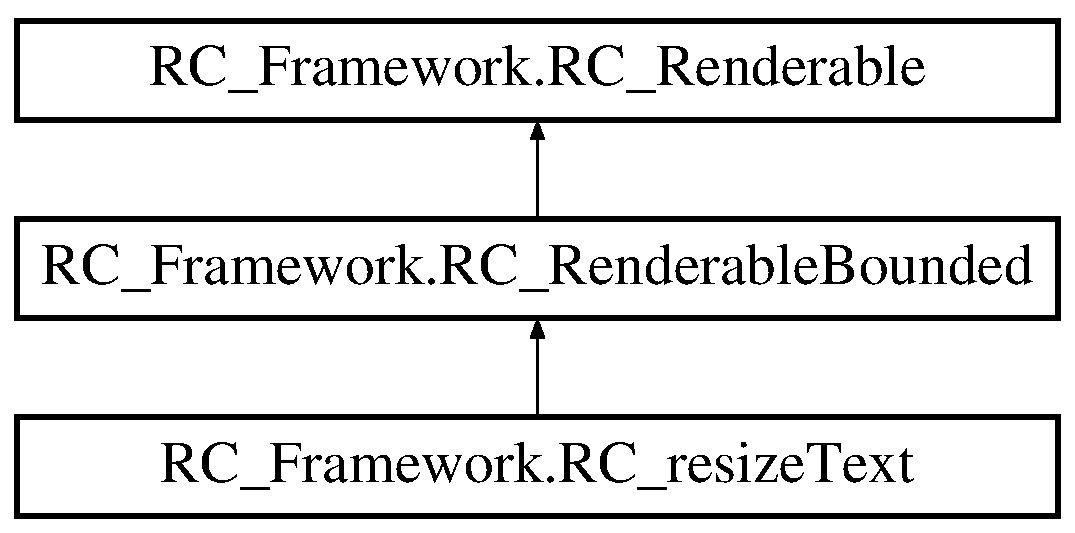
\includegraphics[height=3.000000cm]{class_r_c___framework_1_1_r_c__resize_text}
\end{center}
\end{figure}
\subsection*{Public Member Functions}
\begin{DoxyCompactItemize}
\item 
\mbox{\hyperlink{class_r_c___framework_1_1_r_c__resize_text_a177f87e9f41967dae29a97e27b3defd2}{R\+C\+\_\+resize\+Text}} (Graphics\+Device gd, string textZ, Rectangle \mbox{\hyperlink{class_r_c___framework_1_1_r_c___renderable_bounded_aabcb0f8cd56a2e7b6209f8530194aff1}{boundz}}, Color back\+Ground\+Color, Color foreground\+Color)
\begin{DoxyCompactList}\small\item\em Single line of text thats resizable and bounded if you male the foreground\+Color white then the white font can be re-\/coloured on draw if you set colour \end{DoxyCompactList}\item 
override void \mbox{\hyperlink{class_r_c___framework_1_1_r_c__resize_text_aa591010e25943e1c1a45555cecaa8fcc}{Draw}} (Sprite\+Batch sb)
\begin{DoxyCompactList}\small\item\em Standard draw routine which assumes the renderable knows where it is \end{DoxyCompactList}\end{DoxyCompactItemize}
\subsection*{Properties}
\begin{DoxyCompactItemize}
\item 
Rectangle \mbox{\hyperlink{class_r_c___framework_1_1_r_c__resize_text_a2fdff93da1c5820e14fdc49cb223d54f}{dest}}\hspace{0.3cm}{\ttfamily  \mbox{[}get, set\mbox{]}}
\end{DoxyCompactItemize}
\subsection*{Additional Inherited Members}


\subsection{Constructor \& Destructor Documentation}
\mbox{\Hypertarget{class_r_c___framework_1_1_r_c__resize_text_a177f87e9f41967dae29a97e27b3defd2}\label{class_r_c___framework_1_1_r_c__resize_text_a177f87e9f41967dae29a97e27b3defd2}} 
\index{R\+C\+\_\+\+Framework\+::\+R\+C\+\_\+resize\+Text@{R\+C\+\_\+\+Framework\+::\+R\+C\+\_\+resize\+Text}!R\+C\+\_\+resize\+Text@{R\+C\+\_\+resize\+Text}}
\index{R\+C\+\_\+resize\+Text@{R\+C\+\_\+resize\+Text}!R\+C\+\_\+\+Framework\+::\+R\+C\+\_\+resize\+Text@{R\+C\+\_\+\+Framework\+::\+R\+C\+\_\+resize\+Text}}
\subsubsection{\texorpdfstring{R\+C\+\_\+resize\+Text()}{RC\_resizeText()}}
{\footnotesize\ttfamily R\+C\+\_\+\+Framework.\+R\+C\+\_\+resize\+Text.\+R\+C\+\_\+resize\+Text (\begin{DoxyParamCaption}\item[{Graphics\+Device}]{gd,  }\item[{string}]{textZ,  }\item[{Rectangle}]{boundz,  }\item[{Color}]{back\+Ground\+Color,  }\item[{Color}]{foreground\+Color }\end{DoxyParamCaption})}



Single line of text thats resizable and bounded if you male the foreground\+Color white then the white font can be re-\/coloured on draw if you set colour 


\begin{DoxyParams}{Parameters}
{\em gd} & \\
\hline
{\em textZ} & \\
\hline
{\em boundz} & \\
\hline
{\em back\+Ground\+Color} & \\
\hline
{\em foreground\+Color} & \\
\hline
\end{DoxyParams}


\subsection{Member Function Documentation}
\mbox{\Hypertarget{class_r_c___framework_1_1_r_c__resize_text_aa591010e25943e1c1a45555cecaa8fcc}\label{class_r_c___framework_1_1_r_c__resize_text_aa591010e25943e1c1a45555cecaa8fcc}} 
\index{R\+C\+\_\+\+Framework\+::\+R\+C\+\_\+resize\+Text@{R\+C\+\_\+\+Framework\+::\+R\+C\+\_\+resize\+Text}!Draw@{Draw}}
\index{Draw@{Draw}!R\+C\+\_\+\+Framework\+::\+R\+C\+\_\+resize\+Text@{R\+C\+\_\+\+Framework\+::\+R\+C\+\_\+resize\+Text}}
\subsubsection{\texorpdfstring{Draw()}{Draw()}}
{\footnotesize\ttfamily override void R\+C\+\_\+\+Framework.\+R\+C\+\_\+resize\+Text.\+Draw (\begin{DoxyParamCaption}\item[{Sprite\+Batch}]{sb }\end{DoxyParamCaption})\hspace{0.3cm}{\ttfamily [virtual]}}



Standard draw routine which assumes the renderable knows where it is 


\begin{DoxyParams}{Parameters}
{\em sb} & \\
\hline
\end{DoxyParams}


Reimplemented from \mbox{\hyperlink{class_r_c___framework_1_1_r_c___renderable_acc26db34e382a25a989c4c0dd0354b23}{R\+C\+\_\+\+Framework.\+R\+C\+\_\+\+Renderable}}.



\subsection{Property Documentation}
\mbox{\Hypertarget{class_r_c___framework_1_1_r_c__resize_text_a2fdff93da1c5820e14fdc49cb223d54f}\label{class_r_c___framework_1_1_r_c__resize_text_a2fdff93da1c5820e14fdc49cb223d54f}} 
\index{R\+C\+\_\+\+Framework\+::\+R\+C\+\_\+resize\+Text@{R\+C\+\_\+\+Framework\+::\+R\+C\+\_\+resize\+Text}!dest@{dest}}
\index{dest@{dest}!R\+C\+\_\+\+Framework\+::\+R\+C\+\_\+resize\+Text@{R\+C\+\_\+\+Framework\+::\+R\+C\+\_\+resize\+Text}}
\subsubsection{\texorpdfstring{dest}{dest}}
{\footnotesize\ttfamily Rectangle R\+C\+\_\+\+Framework.\+R\+C\+\_\+resize\+Text.\+dest\hspace{0.3cm}{\ttfamily [get]}, {\ttfamily [set]}}



The documentation for this class was generated from the following file\+:\begin{DoxyCompactItemize}
\item 
F\+:/\+B/\+R\+C\+\_\+\+Framework2018/\+Source/\mbox{\hyperlink{_r_c___renderables_util_text_8cs}{R\+C\+\_\+\+Renderables\+Util\+Text.\+cs}}\end{DoxyCompactItemize}

\hypertarget{class_r_c___framework_1_1_r_c___surface}{}\section{R\+C\+\_\+\+Framework.\+R\+C\+\_\+\+Surface Class Reference}
\label{class_r_c___framework_1_1_r_c___surface}\index{R\+C\+\_\+\+Framework.\+R\+C\+\_\+\+Surface@{R\+C\+\_\+\+Framework.\+R\+C\+\_\+\+Surface}}


The Purpose of this class is to provide a canvas (perhaps it sould have been labled R\+C\+\_\+canvas) It provides a few routines to work with actual pixels witout needing to load an image use \mbox{\hyperlink{class_r_c___framework_1_1_r_c___surface_a88a1b5fd5ab87f2f3cdb9bf0bc825ffc}{create\+Tex(\+Graphics\+Device device)}} to convert it to a texture which is what you need to actually render the surface Surfaces are always rectanglar  


\subsection*{Public Member Functions}
\begin{DoxyCompactItemize}
\item 
\mbox{\hyperlink{class_r_c___framework_1_1_r_c___surface_aa0ebfc848c2efcf738168ba4ae24a700}{R\+C\+\_\+\+Surface}} ()
\begin{DoxyCompactList}\small\item\em Default constructor produces 1 white pixel the idea being that you then run init to get a meaningfull surface \end{DoxyCompactList}\item 
\mbox{\hyperlink{class_r_c___framework_1_1_r_c___surface_a8cf9c7bd5f30e2ce9a6fe58fb64cd301}{R\+C\+\_\+\+Surface}} (int width, int height, Color c)
\item 
\mbox{\hyperlink{class_r_c___framework_1_1_r_c___surface_ada89bd248fe4aea65a1cd8f579f17fa1}{R\+C\+\_\+\+Surface}} (int width, int height, Color top\+LeftC, Color top\+RightC, Color bot\+LeftC, Color bot\+RightC)
\item 
\mbox{\hyperlink{class_r_c___framework_1_1_r_c___surface_ad5778d6547c7ecca1f0c35264a71f7d5}{R\+C\+\_\+\+Surface}} (String\mbox{[}$\,$\mbox{]} lines, Color\mbox{[}$\,$\mbox{]} pal, String pal\+Index)
\item 
\mbox{\hyperlink{class_r_c___framework_1_1_r_c___surface_ac79ed2e2afed744ec647c8e3587bfc17}{R\+C\+\_\+\+Surface}} (\mbox{\hyperlink{class_r_c___framework_1_1_r_c___surface}{R\+C\+\_\+\+Surface}} sur, int x\+Factor, int y\+Factor, int x\+Gap, int y\+Gap, Color def\+Color, int x\+Pad, int y\+Pad)
\begin{DoxyCompactList}\small\item\em Enlarges a surface -\/ possibly with a gap between pixels and with the possibility of padding it out a bit to get a power of 2 \end{DoxyCompactList}\item 
void \mbox{\hyperlink{class_r_c___framework_1_1_r_c___surface_a88c34f3e232de3dd02f82c3145239553}{init}} (int width, int height, Color top\+LeftC, Color top\+RightC, Color bot\+LeftC, Color bot\+RightC)
\begin{DoxyCompactList}\small\item\em Initialise a colour field with a diferent colour at each corner \end{DoxyCompactList}\item 
void \mbox{\hyperlink{class_r_c___framework_1_1_r_c___surface_a163695b3e6c5df4a9cbacc5d3f33ab44}{set\+Color}} (int x, int y, Color c)
\begin{DoxyCompactList}\small\item\em Set a pixel colour \end{DoxyCompactList}\item 
Color \mbox{\hyperlink{class_r_c___framework_1_1_r_c___surface_acafd7281d388d077a1b1afaea6743718}{get\+Color}} (int x, int y)
\begin{DoxyCompactList}\small\item\em get or retreive a pixel colour \end{DoxyCompactList}\item 
void \mbox{\hyperlink{class_r_c___framework_1_1_r_c___surface_a131d4ac4006056b9e6a62ae82aaae603}{set\+In\+Texture2D}} (Texture2D tex)
\begin{DoxyCompactList}\small\item\em Copies the surface to an already existing texture \end{DoxyCompactList}\item 
void \mbox{\hyperlink{class_r_c___framework_1_1_r_c___surface_a93d79ef4363e12e80a454dc49a80770a}{get\+From\+Texture2D}} (Texture2D tex)
\begin{DoxyCompactList}\small\item\em gets pixel data from an existing texture \end{DoxyCompactList}\item 
void \mbox{\hyperlink{class_r_c___framework_1_1_r_c___surface_abab645c5b58a88c3b1e13d1624163272}{add\+Line\+Rectangle}} (Rectangle r, Color c)
\begin{DoxyCompactList}\small\item\em Draws a 1 pixel wide rectangle of a given colour on the surface \end{DoxyCompactList}\item 
void \mbox{\hyperlink{class_r_c___framework_1_1_r_c___surface_a93af5231a5d6cb46ce86fc9895a3cd29}{add\+Fill\+Rectangle}} (Rectangle r, Color c)
\begin{DoxyCompactList}\small\item\em Draws a filled rectangle of a given colour (can be slow. it often is if its any significant size) \end{DoxyCompactList}\item 
void \mbox{\hyperlink{class_r_c___framework_1_1_r_c___surface_adc92e7c233e99edec13e4831b413a531}{set\+Color}} (Color c)
\begin{DoxyCompactList}\small\item\em Sets a colour in the entire surface \end{DoxyCompactList}\item 
void \mbox{\hyperlink{class_r_c___framework_1_1_r_c___surface_afe965ef242eba8173932ac8bc19ec6e9}{add\+Border}} (int border\+Width, Color border\+Color)
\begin{DoxyCompactList}\small\item\em Draws a coloured border on the surface \end{DoxyCompactList}\item 
void \mbox{\hyperlink{class_r_c___framework_1_1_r_c___surface_ad16458caf26de6edba572ce3ac85342c}{add\+Sculpted\+Border}} (Rectangle r, Color c\+Left\+Top, Color c\+Bot\+Right, int b\+Width)
\begin{DoxyCompactList}\small\item\em Adds a border in which the top and left are a diferent colour to the rest of the border can be used to create a 3D look \end{DoxyCompactList}\item 
void \mbox{\hyperlink{class_r_c___framework_1_1_r_c___surface_ad339e6a77515c0d9a59f55f886246a9d}{draw\+Hline}} (int x1, int y, int x2, Color x1C, Color x2C)
\begin{DoxyCompactList}\small\item\em Draws a horizontal line \end{DoxyCompactList}\item 
void \mbox{\hyperlink{class_r_c___framework_1_1_r_c___surface_adfa7830cd882206d779179da1a9622ac}{draw\+Vline}} (int x, int y1, int y2, Color y1C, Color y2C)
\begin{DoxyCompactList}\small\item\em Draws a vertical line \end{DoxyCompactList}\item 
Texture2D \mbox{\hyperlink{class_r_c___framework_1_1_r_c___surface_a88a1b5fd5ab87f2f3cdb9bf0bc825ffc}{create\+Tex}} (Graphics\+Device device)
\begin{DoxyCompactList}\small\item\em creates a new texture that has a copy of the existing surface image \end{DoxyCompactList}\end{DoxyCompactItemize}


\subsection{Detailed Description}
The Purpose of this class is to provide a canvas (perhaps it sould have been labled R\+C\+\_\+canvas) It provides a few routines to work with actual pixels witout needing to load an image use \mbox{\hyperlink{class_r_c___framework_1_1_r_c___surface_a88a1b5fd5ab87f2f3cdb9bf0bc825ffc}{create\+Tex(\+Graphics\+Device device)}} to convert it to a texture which is what you need to actually render the surface Surfaces are always rectanglar 



\subsection{Constructor \& Destructor Documentation}
\mbox{\Hypertarget{class_r_c___framework_1_1_r_c___surface_aa0ebfc848c2efcf738168ba4ae24a700}\label{class_r_c___framework_1_1_r_c___surface_aa0ebfc848c2efcf738168ba4ae24a700}} 
\index{R\+C\+\_\+\+Framework\+::\+R\+C\+\_\+\+Surface@{R\+C\+\_\+\+Framework\+::\+R\+C\+\_\+\+Surface}!R\+C\+\_\+\+Surface@{R\+C\+\_\+\+Surface}}
\index{R\+C\+\_\+\+Surface@{R\+C\+\_\+\+Surface}!R\+C\+\_\+\+Framework\+::\+R\+C\+\_\+\+Surface@{R\+C\+\_\+\+Framework\+::\+R\+C\+\_\+\+Surface}}
\subsubsection{\texorpdfstring{R\+C\+\_\+\+Surface()}{RC\_Surface()}\hspace{0.1cm}{\footnotesize\ttfamily [1/5]}}
{\footnotesize\ttfamily R\+C\+\_\+\+Framework.\+R\+C\+\_\+\+Surface.\+R\+C\+\_\+\+Surface (\begin{DoxyParamCaption}{ }\end{DoxyParamCaption})}



Default constructor produces 1 white pixel the idea being that you then run init to get a meaningfull surface 

\mbox{\Hypertarget{class_r_c___framework_1_1_r_c___surface_a8cf9c7bd5f30e2ce9a6fe58fb64cd301}\label{class_r_c___framework_1_1_r_c___surface_a8cf9c7bd5f30e2ce9a6fe58fb64cd301}} 
\index{R\+C\+\_\+\+Framework\+::\+R\+C\+\_\+\+Surface@{R\+C\+\_\+\+Framework\+::\+R\+C\+\_\+\+Surface}!R\+C\+\_\+\+Surface@{R\+C\+\_\+\+Surface}}
\index{R\+C\+\_\+\+Surface@{R\+C\+\_\+\+Surface}!R\+C\+\_\+\+Framework\+::\+R\+C\+\_\+\+Surface@{R\+C\+\_\+\+Framework\+::\+R\+C\+\_\+\+Surface}}
\subsubsection{\texorpdfstring{R\+C\+\_\+\+Surface()}{RC\_Surface()}\hspace{0.1cm}{\footnotesize\ttfamily [2/5]}}
{\footnotesize\ttfamily R\+C\+\_\+\+Framework.\+R\+C\+\_\+\+Surface.\+R\+C\+\_\+\+Surface (\begin{DoxyParamCaption}\item[{int}]{width,  }\item[{int}]{height,  }\item[{Color}]{c }\end{DoxyParamCaption})}

\mbox{\Hypertarget{class_r_c___framework_1_1_r_c___surface_ada89bd248fe4aea65a1cd8f579f17fa1}\label{class_r_c___framework_1_1_r_c___surface_ada89bd248fe4aea65a1cd8f579f17fa1}} 
\index{R\+C\+\_\+\+Framework\+::\+R\+C\+\_\+\+Surface@{R\+C\+\_\+\+Framework\+::\+R\+C\+\_\+\+Surface}!R\+C\+\_\+\+Surface@{R\+C\+\_\+\+Surface}}
\index{R\+C\+\_\+\+Surface@{R\+C\+\_\+\+Surface}!R\+C\+\_\+\+Framework\+::\+R\+C\+\_\+\+Surface@{R\+C\+\_\+\+Framework\+::\+R\+C\+\_\+\+Surface}}
\subsubsection{\texorpdfstring{R\+C\+\_\+\+Surface()}{RC\_Surface()}\hspace{0.1cm}{\footnotesize\ttfamily [3/5]}}
{\footnotesize\ttfamily R\+C\+\_\+\+Framework.\+R\+C\+\_\+\+Surface.\+R\+C\+\_\+\+Surface (\begin{DoxyParamCaption}\item[{int}]{width,  }\item[{int}]{height,  }\item[{Color}]{top\+LeftC,  }\item[{Color}]{top\+RightC,  }\item[{Color}]{bot\+LeftC,  }\item[{Color}]{bot\+RightC }\end{DoxyParamCaption})}

\mbox{\Hypertarget{class_r_c___framework_1_1_r_c___surface_ad5778d6547c7ecca1f0c35264a71f7d5}\label{class_r_c___framework_1_1_r_c___surface_ad5778d6547c7ecca1f0c35264a71f7d5}} 
\index{R\+C\+\_\+\+Framework\+::\+R\+C\+\_\+\+Surface@{R\+C\+\_\+\+Framework\+::\+R\+C\+\_\+\+Surface}!R\+C\+\_\+\+Surface@{R\+C\+\_\+\+Surface}}
\index{R\+C\+\_\+\+Surface@{R\+C\+\_\+\+Surface}!R\+C\+\_\+\+Framework\+::\+R\+C\+\_\+\+Surface@{R\+C\+\_\+\+Framework\+::\+R\+C\+\_\+\+Surface}}
\subsubsection{\texorpdfstring{R\+C\+\_\+\+Surface()}{RC\_Surface()}\hspace{0.1cm}{\footnotesize\ttfamily [4/5]}}
{\footnotesize\ttfamily R\+C\+\_\+\+Framework.\+R\+C\+\_\+\+Surface.\+R\+C\+\_\+\+Surface (\begin{DoxyParamCaption}\item[{String \mbox{[}$\,$\mbox{]}}]{lines,  }\item[{Color \mbox{[}$\,$\mbox{]}}]{pal,  }\item[{String}]{pal\+Index }\end{DoxyParamCaption})}

\mbox{\Hypertarget{class_r_c___framework_1_1_r_c___surface_ac79ed2e2afed744ec647c8e3587bfc17}\label{class_r_c___framework_1_1_r_c___surface_ac79ed2e2afed744ec647c8e3587bfc17}} 
\index{R\+C\+\_\+\+Framework\+::\+R\+C\+\_\+\+Surface@{R\+C\+\_\+\+Framework\+::\+R\+C\+\_\+\+Surface}!R\+C\+\_\+\+Surface@{R\+C\+\_\+\+Surface}}
\index{R\+C\+\_\+\+Surface@{R\+C\+\_\+\+Surface}!R\+C\+\_\+\+Framework\+::\+R\+C\+\_\+\+Surface@{R\+C\+\_\+\+Framework\+::\+R\+C\+\_\+\+Surface}}
\subsubsection{\texorpdfstring{R\+C\+\_\+\+Surface()}{RC\_Surface()}\hspace{0.1cm}{\footnotesize\ttfamily [5/5]}}
{\footnotesize\ttfamily R\+C\+\_\+\+Framework.\+R\+C\+\_\+\+Surface.\+R\+C\+\_\+\+Surface (\begin{DoxyParamCaption}\item[{\mbox{\hyperlink{class_r_c___framework_1_1_r_c___surface}{R\+C\+\_\+\+Surface}}}]{sur,  }\item[{int}]{x\+Factor,  }\item[{int}]{y\+Factor,  }\item[{int}]{x\+Gap,  }\item[{int}]{y\+Gap,  }\item[{Color}]{def\+Color,  }\item[{int}]{x\+Pad,  }\item[{int}]{y\+Pad }\end{DoxyParamCaption})}



Enlarges a surface -\/ possibly with a gap between pixels and with the possibility of padding it out a bit to get a power of 2 


\begin{DoxyParams}{Parameters}
{\em sur} & \\
\hline
{\em x\+Factor} & \\
\hline
{\em y\+Factor} & \\
\hline
{\em x\+Gap} & \\
\hline
{\em y\+Gap} & \\
\hline
{\em def\+Color} & \\
\hline
{\em x\+Pad} & \\
\hline
{\em y\+Pad} & \\
\hline
\end{DoxyParams}


\subsection{Member Function Documentation}
\mbox{\Hypertarget{class_r_c___framework_1_1_r_c___surface_afe965ef242eba8173932ac8bc19ec6e9}\label{class_r_c___framework_1_1_r_c___surface_afe965ef242eba8173932ac8bc19ec6e9}} 
\index{R\+C\+\_\+\+Framework\+::\+R\+C\+\_\+\+Surface@{R\+C\+\_\+\+Framework\+::\+R\+C\+\_\+\+Surface}!add\+Border@{add\+Border}}
\index{add\+Border@{add\+Border}!R\+C\+\_\+\+Framework\+::\+R\+C\+\_\+\+Surface@{R\+C\+\_\+\+Framework\+::\+R\+C\+\_\+\+Surface}}
\subsubsection{\texorpdfstring{add\+Border()}{addBorder()}}
{\footnotesize\ttfamily void R\+C\+\_\+\+Framework.\+R\+C\+\_\+\+Surface.\+add\+Border (\begin{DoxyParamCaption}\item[{int}]{border\+Width,  }\item[{Color}]{border\+Color }\end{DoxyParamCaption})}



Draws a coloured border on the surface 


\begin{DoxyParams}{Parameters}
{\em border\+Width} & \\
\hline
{\em border\+Color} & \\
\hline
\end{DoxyParams}
\mbox{\Hypertarget{class_r_c___framework_1_1_r_c___surface_a93af5231a5d6cb46ce86fc9895a3cd29}\label{class_r_c___framework_1_1_r_c___surface_a93af5231a5d6cb46ce86fc9895a3cd29}} 
\index{R\+C\+\_\+\+Framework\+::\+R\+C\+\_\+\+Surface@{R\+C\+\_\+\+Framework\+::\+R\+C\+\_\+\+Surface}!add\+Fill\+Rectangle@{add\+Fill\+Rectangle}}
\index{add\+Fill\+Rectangle@{add\+Fill\+Rectangle}!R\+C\+\_\+\+Framework\+::\+R\+C\+\_\+\+Surface@{R\+C\+\_\+\+Framework\+::\+R\+C\+\_\+\+Surface}}
\subsubsection{\texorpdfstring{add\+Fill\+Rectangle()}{addFillRectangle()}}
{\footnotesize\ttfamily void R\+C\+\_\+\+Framework.\+R\+C\+\_\+\+Surface.\+add\+Fill\+Rectangle (\begin{DoxyParamCaption}\item[{Rectangle}]{r,  }\item[{Color}]{c }\end{DoxyParamCaption})}



Draws a filled rectangle of a given colour (can be slow. it often is if its any significant size) 


\begin{DoxyParams}{Parameters}
{\em r} & \\
\hline
{\em c} & \\
\hline
\end{DoxyParams}
\mbox{\Hypertarget{class_r_c___framework_1_1_r_c___surface_abab645c5b58a88c3b1e13d1624163272}\label{class_r_c___framework_1_1_r_c___surface_abab645c5b58a88c3b1e13d1624163272}} 
\index{R\+C\+\_\+\+Framework\+::\+R\+C\+\_\+\+Surface@{R\+C\+\_\+\+Framework\+::\+R\+C\+\_\+\+Surface}!add\+Line\+Rectangle@{add\+Line\+Rectangle}}
\index{add\+Line\+Rectangle@{add\+Line\+Rectangle}!R\+C\+\_\+\+Framework\+::\+R\+C\+\_\+\+Surface@{R\+C\+\_\+\+Framework\+::\+R\+C\+\_\+\+Surface}}
\subsubsection{\texorpdfstring{add\+Line\+Rectangle()}{addLineRectangle()}}
{\footnotesize\ttfamily void R\+C\+\_\+\+Framework.\+R\+C\+\_\+\+Surface.\+add\+Line\+Rectangle (\begin{DoxyParamCaption}\item[{Rectangle}]{r,  }\item[{Color}]{c }\end{DoxyParamCaption})}



Draws a 1 pixel wide rectangle of a given colour on the surface 


\begin{DoxyParams}{Parameters}
{\em r} & \\
\hline
{\em c} & \\
\hline
\end{DoxyParams}
\mbox{\Hypertarget{class_r_c___framework_1_1_r_c___surface_ad16458caf26de6edba572ce3ac85342c}\label{class_r_c___framework_1_1_r_c___surface_ad16458caf26de6edba572ce3ac85342c}} 
\index{R\+C\+\_\+\+Framework\+::\+R\+C\+\_\+\+Surface@{R\+C\+\_\+\+Framework\+::\+R\+C\+\_\+\+Surface}!add\+Sculpted\+Border@{add\+Sculpted\+Border}}
\index{add\+Sculpted\+Border@{add\+Sculpted\+Border}!R\+C\+\_\+\+Framework\+::\+R\+C\+\_\+\+Surface@{R\+C\+\_\+\+Framework\+::\+R\+C\+\_\+\+Surface}}
\subsubsection{\texorpdfstring{add\+Sculpted\+Border()}{addSculptedBorder()}}
{\footnotesize\ttfamily void R\+C\+\_\+\+Framework.\+R\+C\+\_\+\+Surface.\+add\+Sculpted\+Border (\begin{DoxyParamCaption}\item[{Rectangle}]{r,  }\item[{Color}]{c\+Left\+Top,  }\item[{Color}]{c\+Bot\+Right,  }\item[{int}]{b\+Width }\end{DoxyParamCaption})}



Adds a border in which the top and left are a diferent colour to the rest of the border can be used to create a 3D look 

The following lines are a hint on how to get a 3d border look Color c\+Light = \mbox{\hyperlink{class_r_c___framework_1_1_util_a88559e70851ee1e21bdc1375b862919d}{Util.\+lighter\+Or\+Darker}}(c, 1.\+4f); Color c\+Dark = \mbox{\hyperlink{class_r_c___framework_1_1_util_a88559e70851ee1e21bdc1375b862919d}{Util.\+lighter\+Or\+Darker}}(c, 0.\+6f); 


\begin{DoxyParams}{Parameters}
{\em r} & \\
\hline
{\em c\+Left\+Top} & \\
\hline
{\em c\+Bot\+Right} & \\
\hline
{\em b\+Width} & \\
\hline
\end{DoxyParams}
\mbox{\Hypertarget{class_r_c___framework_1_1_r_c___surface_a88a1b5fd5ab87f2f3cdb9bf0bc825ffc}\label{class_r_c___framework_1_1_r_c___surface_a88a1b5fd5ab87f2f3cdb9bf0bc825ffc}} 
\index{R\+C\+\_\+\+Framework\+::\+R\+C\+\_\+\+Surface@{R\+C\+\_\+\+Framework\+::\+R\+C\+\_\+\+Surface}!create\+Tex@{create\+Tex}}
\index{create\+Tex@{create\+Tex}!R\+C\+\_\+\+Framework\+::\+R\+C\+\_\+\+Surface@{R\+C\+\_\+\+Framework\+::\+R\+C\+\_\+\+Surface}}
\subsubsection{\texorpdfstring{create\+Tex()}{createTex()}}
{\footnotesize\ttfamily Texture2D R\+C\+\_\+\+Framework.\+R\+C\+\_\+\+Surface.\+create\+Tex (\begin{DoxyParamCaption}\item[{Graphics\+Device}]{device }\end{DoxyParamCaption})}



creates a new texture that has a copy of the existing surface image 


\begin{DoxyParams}{Parameters}
{\em device} & \\
\hline
\end{DoxyParams}
\begin{DoxyReturn}{Returns}

\end{DoxyReturn}
\mbox{\Hypertarget{class_r_c___framework_1_1_r_c___surface_ad339e6a77515c0d9a59f55f886246a9d}\label{class_r_c___framework_1_1_r_c___surface_ad339e6a77515c0d9a59f55f886246a9d}} 
\index{R\+C\+\_\+\+Framework\+::\+R\+C\+\_\+\+Surface@{R\+C\+\_\+\+Framework\+::\+R\+C\+\_\+\+Surface}!draw\+Hline@{draw\+Hline}}
\index{draw\+Hline@{draw\+Hline}!R\+C\+\_\+\+Framework\+::\+R\+C\+\_\+\+Surface@{R\+C\+\_\+\+Framework\+::\+R\+C\+\_\+\+Surface}}
\subsubsection{\texorpdfstring{draw\+Hline()}{drawHline()}}
{\footnotesize\ttfamily void R\+C\+\_\+\+Framework.\+R\+C\+\_\+\+Surface.\+draw\+Hline (\begin{DoxyParamCaption}\item[{int}]{x1,  }\item[{int}]{y,  }\item[{int}]{x2,  }\item[{Color}]{x1C,  }\item[{Color}]{x2C }\end{DoxyParamCaption})}



Draws a horizontal line 


\begin{DoxyParams}{Parameters}
{\em x1} & \\
\hline
{\em y} & \\
\hline
{\em x2} & \\
\hline
{\em x1C} & \\
\hline
{\em x2C} & \\
\hline
\end{DoxyParams}
\mbox{\Hypertarget{class_r_c___framework_1_1_r_c___surface_adfa7830cd882206d779179da1a9622ac}\label{class_r_c___framework_1_1_r_c___surface_adfa7830cd882206d779179da1a9622ac}} 
\index{R\+C\+\_\+\+Framework\+::\+R\+C\+\_\+\+Surface@{R\+C\+\_\+\+Framework\+::\+R\+C\+\_\+\+Surface}!draw\+Vline@{draw\+Vline}}
\index{draw\+Vline@{draw\+Vline}!R\+C\+\_\+\+Framework\+::\+R\+C\+\_\+\+Surface@{R\+C\+\_\+\+Framework\+::\+R\+C\+\_\+\+Surface}}
\subsubsection{\texorpdfstring{draw\+Vline()}{drawVline()}}
{\footnotesize\ttfamily void R\+C\+\_\+\+Framework.\+R\+C\+\_\+\+Surface.\+draw\+Vline (\begin{DoxyParamCaption}\item[{int}]{x,  }\item[{int}]{y1,  }\item[{int}]{y2,  }\item[{Color}]{y1C,  }\item[{Color}]{y2C }\end{DoxyParamCaption})}



Draws a vertical line 


\begin{DoxyParams}{Parameters}
{\em x} & \\
\hline
{\em y1} & \\
\hline
{\em y2} & \\
\hline
{\em y1C} & \\
\hline
{\em y2C} & \\
\hline
\end{DoxyParams}
\mbox{\Hypertarget{class_r_c___framework_1_1_r_c___surface_acafd7281d388d077a1b1afaea6743718}\label{class_r_c___framework_1_1_r_c___surface_acafd7281d388d077a1b1afaea6743718}} 
\index{R\+C\+\_\+\+Framework\+::\+R\+C\+\_\+\+Surface@{R\+C\+\_\+\+Framework\+::\+R\+C\+\_\+\+Surface}!get\+Color@{get\+Color}}
\index{get\+Color@{get\+Color}!R\+C\+\_\+\+Framework\+::\+R\+C\+\_\+\+Surface@{R\+C\+\_\+\+Framework\+::\+R\+C\+\_\+\+Surface}}
\subsubsection{\texorpdfstring{get\+Color()}{getColor()}}
{\footnotesize\ttfamily Color R\+C\+\_\+\+Framework.\+R\+C\+\_\+\+Surface.\+get\+Color (\begin{DoxyParamCaption}\item[{int}]{x,  }\item[{int}]{y }\end{DoxyParamCaption})}



get or retreive a pixel colour 


\begin{DoxyParams}{Parameters}
{\em x} & \\
\hline
{\em y} & \\
\hline
\end{DoxyParams}
\begin{DoxyReturn}{Returns}

\end{DoxyReturn}
\mbox{\Hypertarget{class_r_c___framework_1_1_r_c___surface_a93d79ef4363e12e80a454dc49a80770a}\label{class_r_c___framework_1_1_r_c___surface_a93d79ef4363e12e80a454dc49a80770a}} 
\index{R\+C\+\_\+\+Framework\+::\+R\+C\+\_\+\+Surface@{R\+C\+\_\+\+Framework\+::\+R\+C\+\_\+\+Surface}!get\+From\+Texture2D@{get\+From\+Texture2D}}
\index{get\+From\+Texture2D@{get\+From\+Texture2D}!R\+C\+\_\+\+Framework\+::\+R\+C\+\_\+\+Surface@{R\+C\+\_\+\+Framework\+::\+R\+C\+\_\+\+Surface}}
\subsubsection{\texorpdfstring{get\+From\+Texture2\+D()}{getFromTexture2D()}}
{\footnotesize\ttfamily void R\+C\+\_\+\+Framework.\+R\+C\+\_\+\+Surface.\+get\+From\+Texture2D (\begin{DoxyParamCaption}\item[{Texture2D}]{tex }\end{DoxyParamCaption})}



gets pixel data from an existing texture 


\begin{DoxyParams}{Parameters}
{\em tex} & \\
\hline
\end{DoxyParams}
\mbox{\Hypertarget{class_r_c___framework_1_1_r_c___surface_a88c34f3e232de3dd02f82c3145239553}\label{class_r_c___framework_1_1_r_c___surface_a88c34f3e232de3dd02f82c3145239553}} 
\index{R\+C\+\_\+\+Framework\+::\+R\+C\+\_\+\+Surface@{R\+C\+\_\+\+Framework\+::\+R\+C\+\_\+\+Surface}!init@{init}}
\index{init@{init}!R\+C\+\_\+\+Framework\+::\+R\+C\+\_\+\+Surface@{R\+C\+\_\+\+Framework\+::\+R\+C\+\_\+\+Surface}}
\subsubsection{\texorpdfstring{init()}{init()}}
{\footnotesize\ttfamily void R\+C\+\_\+\+Framework.\+R\+C\+\_\+\+Surface.\+init (\begin{DoxyParamCaption}\item[{int}]{width,  }\item[{int}]{height,  }\item[{Color}]{top\+LeftC,  }\item[{Color}]{top\+RightC,  }\item[{Color}]{bot\+LeftC,  }\item[{Color}]{bot\+RightC }\end{DoxyParamCaption})}



Initialise a colour field with a diferent colour at each corner 


\begin{DoxyParams}{Parameters}
{\em width} & \\
\hline
{\em height} & \\
\hline
{\em top\+LeftC} & \\
\hline
{\em top\+RightC} & \\
\hline
{\em bot\+LeftC} & \\
\hline
{\em bot\+RightC} & \\
\hline
\end{DoxyParams}
\mbox{\Hypertarget{class_r_c___framework_1_1_r_c___surface_a163695b3e6c5df4a9cbacc5d3f33ab44}\label{class_r_c___framework_1_1_r_c___surface_a163695b3e6c5df4a9cbacc5d3f33ab44}} 
\index{R\+C\+\_\+\+Framework\+::\+R\+C\+\_\+\+Surface@{R\+C\+\_\+\+Framework\+::\+R\+C\+\_\+\+Surface}!set\+Color@{set\+Color}}
\index{set\+Color@{set\+Color}!R\+C\+\_\+\+Framework\+::\+R\+C\+\_\+\+Surface@{R\+C\+\_\+\+Framework\+::\+R\+C\+\_\+\+Surface}}
\subsubsection{\texorpdfstring{set\+Color()}{setColor()}\hspace{0.1cm}{\footnotesize\ttfamily [1/2]}}
{\footnotesize\ttfamily void R\+C\+\_\+\+Framework.\+R\+C\+\_\+\+Surface.\+set\+Color (\begin{DoxyParamCaption}\item[{int}]{x,  }\item[{int}]{y,  }\item[{Color}]{c }\end{DoxyParamCaption})}



Set a pixel colour 


\begin{DoxyParams}{Parameters}
{\em x} & \\
\hline
{\em y} & \\
\hline
{\em c} & \\
\hline
\end{DoxyParams}
\mbox{\Hypertarget{class_r_c___framework_1_1_r_c___surface_adc92e7c233e99edec13e4831b413a531}\label{class_r_c___framework_1_1_r_c___surface_adc92e7c233e99edec13e4831b413a531}} 
\index{R\+C\+\_\+\+Framework\+::\+R\+C\+\_\+\+Surface@{R\+C\+\_\+\+Framework\+::\+R\+C\+\_\+\+Surface}!set\+Color@{set\+Color}}
\index{set\+Color@{set\+Color}!R\+C\+\_\+\+Framework\+::\+R\+C\+\_\+\+Surface@{R\+C\+\_\+\+Framework\+::\+R\+C\+\_\+\+Surface}}
\subsubsection{\texorpdfstring{set\+Color()}{setColor()}\hspace{0.1cm}{\footnotesize\ttfamily [2/2]}}
{\footnotesize\ttfamily void R\+C\+\_\+\+Framework.\+R\+C\+\_\+\+Surface.\+set\+Color (\begin{DoxyParamCaption}\item[{Color}]{c }\end{DoxyParamCaption})}



Sets a colour in the entire surface 


\begin{DoxyParams}{Parameters}
{\em c} & \\
\hline
\end{DoxyParams}
\mbox{\Hypertarget{class_r_c___framework_1_1_r_c___surface_a131d4ac4006056b9e6a62ae82aaae603}\label{class_r_c___framework_1_1_r_c___surface_a131d4ac4006056b9e6a62ae82aaae603}} 
\index{R\+C\+\_\+\+Framework\+::\+R\+C\+\_\+\+Surface@{R\+C\+\_\+\+Framework\+::\+R\+C\+\_\+\+Surface}!set\+In\+Texture2D@{set\+In\+Texture2D}}
\index{set\+In\+Texture2D@{set\+In\+Texture2D}!R\+C\+\_\+\+Framework\+::\+R\+C\+\_\+\+Surface@{R\+C\+\_\+\+Framework\+::\+R\+C\+\_\+\+Surface}}
\subsubsection{\texorpdfstring{set\+In\+Texture2\+D()}{setInTexture2D()}}
{\footnotesize\ttfamily void R\+C\+\_\+\+Framework.\+R\+C\+\_\+\+Surface.\+set\+In\+Texture2D (\begin{DoxyParamCaption}\item[{Texture2D}]{tex }\end{DoxyParamCaption})}



Copies the surface to an already existing texture 


\begin{DoxyParams}{Parameters}
{\em tex} & \\
\hline
\end{DoxyParams}


The documentation for this class was generated from the following file\+:\begin{DoxyCompactItemize}
\item 
F\+:/\+B/\+R\+C\+\_\+\+Framework2018/\+Source/\mbox{\hyperlink{_r_c___surface_8cs}{R\+C\+\_\+\+Surface.\+cs}}\end{DoxyCompactItemize}

\hypertarget{class_r_c___framework_1_1_r_c___texture}{}\section{R\+C\+\_\+\+Framework.\+R\+C\+\_\+\+Texture Class Reference}
\label{class_r_c___framework_1_1_r_c___texture}\index{R\+C\+\_\+\+Framework.\+R\+C\+\_\+\+Texture@{R\+C\+\_\+\+Framework.\+R\+C\+\_\+\+Texture}}
\subsection*{Public Member Functions}
\begin{DoxyCompactItemize}
\item 
\mbox{\hyperlink{class_r_c___framework_1_1_r_c___texture_a0c6c13c129ff5e69506a72f11f774f63}{R\+C\+\_\+\+Texture}} (string nameQ, string directory\+And\+FilenameQ)
\item 
\mbox{\hyperlink{class_r_c___framework_1_1_r_c___texture_a441e4cb3d98d016c897b3d897ddbcb1d}{R\+C\+\_\+\+Texture}} (string nameQ, string directory\+And\+FilenameQ, int indexQ)
\item 
void \mbox{\hyperlink{class_r_c___framework_1_1_r_c___texture_afa209ab1b5aa0f31309b1476296954ef}{set\+Width\+Height}} (int w, int h)
\item 
bool \mbox{\hyperlink{class_r_c___framework_1_1_r_c___texture_aafec28028905c5864b9a71b7cb19882c}{load\+File}} ()
\item 
void \mbox{\hyperlink{class_r_c___framework_1_1_r_c___texture_a8fec28881bf93c9e2095800b1f59fe2b}{set\+Filename}} ()
\item 
Texture2D \mbox{\hyperlink{class_r_c___framework_1_1_r_c___texture_a41ab7bdcc1a43960fde61e4e8d05f506}{tex}} ()
\item 
Texture2D \mbox{\hyperlink{class_r_c___framework_1_1_r_c___texture_a5518e74f8fe6031830dfac12fb34e531}{Tex}} ()
\end{DoxyCompactItemize}
\subsection*{Static Public Member Functions}
\begin{DoxyCompactItemize}
\item 
static void \mbox{\hyperlink{class_r_c___framework_1_1_r_c___texture_a3d92372e45bb35d42dc5466fde6941c7}{set\+Graphics\+Device}} (Graphics\+Device gdQ)
\end{DoxyCompactItemize}
\subsection*{Public Attributes}
\begin{DoxyCompactItemize}
\item 
string \mbox{\hyperlink{class_r_c___framework_1_1_r_c___texture_abc7884bbd6c745fc9fc5ff89565f3548}{name}} =\char`\"{}\char`\"{}
\item 
string \mbox{\hyperlink{class_r_c___framework_1_1_r_c___texture_a0cbd33116fd5d7a9a75b9b03b4c0ef61}{directory\+And\+Filename}} = \char`\"{}\char`\"{}
\item 
string \mbox{\hyperlink{class_r_c___framework_1_1_r_c___texture_a6f8dc0a89409e325e848fd1a7ddfdbca}{file\+Name}} = \char`\"{}\char`\"{}
\item 
Texture2D \mbox{\hyperlink{class_r_c___framework_1_1_r_c___texture_aa89de08699aa894279bdbd93179ef714}{texQ}} = null
\item 
int \mbox{\hyperlink{class_r_c___framework_1_1_r_c___texture_ab119771404aada6038d4fcface1e63b7}{index}} =0
\item 
int \mbox{\hyperlink{class_r_c___framework_1_1_r_c___texture_afebd93cc0a8c61f387d10759335d94d7}{width\+Active}} =-\/1
\item 
int \mbox{\hyperlink{class_r_c___framework_1_1_r_c___texture_a4fa2fbbe50bd32a923a4f96a93cf59e4}{height\+Active}} =-\/1
\end{DoxyCompactItemize}
\subsection*{Static Public Attributes}
\begin{DoxyCompactItemize}
\item 
static Graphics\+Device \mbox{\hyperlink{class_r_c___framework_1_1_r_c___texture_abdb88e69589307652a7eb98cb6722644}{gd}} =null
\end{DoxyCompactItemize}


\subsection{Constructor \& Destructor Documentation}
\mbox{\Hypertarget{class_r_c___framework_1_1_r_c___texture_a0c6c13c129ff5e69506a72f11f774f63}\label{class_r_c___framework_1_1_r_c___texture_a0c6c13c129ff5e69506a72f11f774f63}} 
\index{R\+C\+\_\+\+Framework\+::\+R\+C\+\_\+\+Texture@{R\+C\+\_\+\+Framework\+::\+R\+C\+\_\+\+Texture}!R\+C\+\_\+\+Texture@{R\+C\+\_\+\+Texture}}
\index{R\+C\+\_\+\+Texture@{R\+C\+\_\+\+Texture}!R\+C\+\_\+\+Framework\+::\+R\+C\+\_\+\+Texture@{R\+C\+\_\+\+Framework\+::\+R\+C\+\_\+\+Texture}}
\subsubsection{\texorpdfstring{R\+C\+\_\+\+Texture()}{RC\_Texture()}\hspace{0.1cm}{\footnotesize\ttfamily [1/2]}}
{\footnotesize\ttfamily R\+C\+\_\+\+Framework.\+R\+C\+\_\+\+Texture.\+R\+C\+\_\+\+Texture (\begin{DoxyParamCaption}\item[{string}]{nameQ,  }\item[{string}]{directory\+And\+FilenameQ }\end{DoxyParamCaption})}

\mbox{\Hypertarget{class_r_c___framework_1_1_r_c___texture_a441e4cb3d98d016c897b3d897ddbcb1d}\label{class_r_c___framework_1_1_r_c___texture_a441e4cb3d98d016c897b3d897ddbcb1d}} 
\index{R\+C\+\_\+\+Framework\+::\+R\+C\+\_\+\+Texture@{R\+C\+\_\+\+Framework\+::\+R\+C\+\_\+\+Texture}!R\+C\+\_\+\+Texture@{R\+C\+\_\+\+Texture}}
\index{R\+C\+\_\+\+Texture@{R\+C\+\_\+\+Texture}!R\+C\+\_\+\+Framework\+::\+R\+C\+\_\+\+Texture@{R\+C\+\_\+\+Framework\+::\+R\+C\+\_\+\+Texture}}
\subsubsection{\texorpdfstring{R\+C\+\_\+\+Texture()}{RC\_Texture()}\hspace{0.1cm}{\footnotesize\ttfamily [2/2]}}
{\footnotesize\ttfamily R\+C\+\_\+\+Framework.\+R\+C\+\_\+\+Texture.\+R\+C\+\_\+\+Texture (\begin{DoxyParamCaption}\item[{string}]{nameQ,  }\item[{string}]{directory\+And\+FilenameQ,  }\item[{int}]{indexQ }\end{DoxyParamCaption})}



\subsection{Member Function Documentation}
\mbox{\Hypertarget{class_r_c___framework_1_1_r_c___texture_aafec28028905c5864b9a71b7cb19882c}\label{class_r_c___framework_1_1_r_c___texture_aafec28028905c5864b9a71b7cb19882c}} 
\index{R\+C\+\_\+\+Framework\+::\+R\+C\+\_\+\+Texture@{R\+C\+\_\+\+Framework\+::\+R\+C\+\_\+\+Texture}!load\+File@{load\+File}}
\index{load\+File@{load\+File}!R\+C\+\_\+\+Framework\+::\+R\+C\+\_\+\+Texture@{R\+C\+\_\+\+Framework\+::\+R\+C\+\_\+\+Texture}}
\subsubsection{\texorpdfstring{load\+File()}{loadFile()}}
{\footnotesize\ttfamily bool R\+C\+\_\+\+Framework.\+R\+C\+\_\+\+Texture.\+load\+File (\begin{DoxyParamCaption}{ }\end{DoxyParamCaption})}

\mbox{\Hypertarget{class_r_c___framework_1_1_r_c___texture_a8fec28881bf93c9e2095800b1f59fe2b}\label{class_r_c___framework_1_1_r_c___texture_a8fec28881bf93c9e2095800b1f59fe2b}} 
\index{R\+C\+\_\+\+Framework\+::\+R\+C\+\_\+\+Texture@{R\+C\+\_\+\+Framework\+::\+R\+C\+\_\+\+Texture}!set\+Filename@{set\+Filename}}
\index{set\+Filename@{set\+Filename}!R\+C\+\_\+\+Framework\+::\+R\+C\+\_\+\+Texture@{R\+C\+\_\+\+Framework\+::\+R\+C\+\_\+\+Texture}}
\subsubsection{\texorpdfstring{set\+Filename()}{setFilename()}}
{\footnotesize\ttfamily void R\+C\+\_\+\+Framework.\+R\+C\+\_\+\+Texture.\+set\+Filename (\begin{DoxyParamCaption}{ }\end{DoxyParamCaption})}

\mbox{\Hypertarget{class_r_c___framework_1_1_r_c___texture_a3d92372e45bb35d42dc5466fde6941c7}\label{class_r_c___framework_1_1_r_c___texture_a3d92372e45bb35d42dc5466fde6941c7}} 
\index{R\+C\+\_\+\+Framework\+::\+R\+C\+\_\+\+Texture@{R\+C\+\_\+\+Framework\+::\+R\+C\+\_\+\+Texture}!set\+Graphics\+Device@{set\+Graphics\+Device}}
\index{set\+Graphics\+Device@{set\+Graphics\+Device}!R\+C\+\_\+\+Framework\+::\+R\+C\+\_\+\+Texture@{R\+C\+\_\+\+Framework\+::\+R\+C\+\_\+\+Texture}}
\subsubsection{\texorpdfstring{set\+Graphics\+Device()}{setGraphicsDevice()}}
{\footnotesize\ttfamily static void R\+C\+\_\+\+Framework.\+R\+C\+\_\+\+Texture.\+set\+Graphics\+Device (\begin{DoxyParamCaption}\item[{Graphics\+Device}]{gdQ }\end{DoxyParamCaption})\hspace{0.3cm}{\ttfamily [static]}}

\mbox{\Hypertarget{class_r_c___framework_1_1_r_c___texture_afa209ab1b5aa0f31309b1476296954ef}\label{class_r_c___framework_1_1_r_c___texture_afa209ab1b5aa0f31309b1476296954ef}} 
\index{R\+C\+\_\+\+Framework\+::\+R\+C\+\_\+\+Texture@{R\+C\+\_\+\+Framework\+::\+R\+C\+\_\+\+Texture}!set\+Width\+Height@{set\+Width\+Height}}
\index{set\+Width\+Height@{set\+Width\+Height}!R\+C\+\_\+\+Framework\+::\+R\+C\+\_\+\+Texture@{R\+C\+\_\+\+Framework\+::\+R\+C\+\_\+\+Texture}}
\subsubsection{\texorpdfstring{set\+Width\+Height()}{setWidthHeight()}}
{\footnotesize\ttfamily void R\+C\+\_\+\+Framework.\+R\+C\+\_\+\+Texture.\+set\+Width\+Height (\begin{DoxyParamCaption}\item[{int}]{w,  }\item[{int}]{h }\end{DoxyParamCaption})}

\mbox{\Hypertarget{class_r_c___framework_1_1_r_c___texture_a41ab7bdcc1a43960fde61e4e8d05f506}\label{class_r_c___framework_1_1_r_c___texture_a41ab7bdcc1a43960fde61e4e8d05f506}} 
\index{R\+C\+\_\+\+Framework\+::\+R\+C\+\_\+\+Texture@{R\+C\+\_\+\+Framework\+::\+R\+C\+\_\+\+Texture}!tex@{tex}}
\index{tex@{tex}!R\+C\+\_\+\+Framework\+::\+R\+C\+\_\+\+Texture@{R\+C\+\_\+\+Framework\+::\+R\+C\+\_\+\+Texture}}
\subsubsection{\texorpdfstring{tex()}{tex()}}
{\footnotesize\ttfamily Texture2D R\+C\+\_\+\+Framework.\+R\+C\+\_\+\+Texture.\+tex (\begin{DoxyParamCaption}{ }\end{DoxyParamCaption})}

\mbox{\Hypertarget{class_r_c___framework_1_1_r_c___texture_a5518e74f8fe6031830dfac12fb34e531}\label{class_r_c___framework_1_1_r_c___texture_a5518e74f8fe6031830dfac12fb34e531}} 
\index{R\+C\+\_\+\+Framework\+::\+R\+C\+\_\+\+Texture@{R\+C\+\_\+\+Framework\+::\+R\+C\+\_\+\+Texture}!Tex@{Tex}}
\index{Tex@{Tex}!R\+C\+\_\+\+Framework\+::\+R\+C\+\_\+\+Texture@{R\+C\+\_\+\+Framework\+::\+R\+C\+\_\+\+Texture}}
\subsubsection{\texorpdfstring{Tex()}{Tex()}}
{\footnotesize\ttfamily Texture2D R\+C\+\_\+\+Framework.\+R\+C\+\_\+\+Texture.\+Tex (\begin{DoxyParamCaption}{ }\end{DoxyParamCaption})}



\subsection{Member Data Documentation}
\mbox{\Hypertarget{class_r_c___framework_1_1_r_c___texture_a0cbd33116fd5d7a9a75b9b03b4c0ef61}\label{class_r_c___framework_1_1_r_c___texture_a0cbd33116fd5d7a9a75b9b03b4c0ef61}} 
\index{R\+C\+\_\+\+Framework\+::\+R\+C\+\_\+\+Texture@{R\+C\+\_\+\+Framework\+::\+R\+C\+\_\+\+Texture}!directory\+And\+Filename@{directory\+And\+Filename}}
\index{directory\+And\+Filename@{directory\+And\+Filename}!R\+C\+\_\+\+Framework\+::\+R\+C\+\_\+\+Texture@{R\+C\+\_\+\+Framework\+::\+R\+C\+\_\+\+Texture}}
\subsubsection{\texorpdfstring{directory\+And\+Filename}{directoryAndFilename}}
{\footnotesize\ttfamily string R\+C\+\_\+\+Framework.\+R\+C\+\_\+\+Texture.\+directory\+And\+Filename = \char`\"{}\char`\"{}}

\mbox{\Hypertarget{class_r_c___framework_1_1_r_c___texture_a6f8dc0a89409e325e848fd1a7ddfdbca}\label{class_r_c___framework_1_1_r_c___texture_a6f8dc0a89409e325e848fd1a7ddfdbca}} 
\index{R\+C\+\_\+\+Framework\+::\+R\+C\+\_\+\+Texture@{R\+C\+\_\+\+Framework\+::\+R\+C\+\_\+\+Texture}!file\+Name@{file\+Name}}
\index{file\+Name@{file\+Name}!R\+C\+\_\+\+Framework\+::\+R\+C\+\_\+\+Texture@{R\+C\+\_\+\+Framework\+::\+R\+C\+\_\+\+Texture}}
\subsubsection{\texorpdfstring{file\+Name}{fileName}}
{\footnotesize\ttfamily string R\+C\+\_\+\+Framework.\+R\+C\+\_\+\+Texture.\+file\+Name = \char`\"{}\char`\"{}}

\mbox{\Hypertarget{class_r_c___framework_1_1_r_c___texture_abdb88e69589307652a7eb98cb6722644}\label{class_r_c___framework_1_1_r_c___texture_abdb88e69589307652a7eb98cb6722644}} 
\index{R\+C\+\_\+\+Framework\+::\+R\+C\+\_\+\+Texture@{R\+C\+\_\+\+Framework\+::\+R\+C\+\_\+\+Texture}!gd@{gd}}
\index{gd@{gd}!R\+C\+\_\+\+Framework\+::\+R\+C\+\_\+\+Texture@{R\+C\+\_\+\+Framework\+::\+R\+C\+\_\+\+Texture}}
\subsubsection{\texorpdfstring{gd}{gd}}
{\footnotesize\ttfamily Graphics\+Device R\+C\+\_\+\+Framework.\+R\+C\+\_\+\+Texture.\+gd =null\hspace{0.3cm}{\ttfamily [static]}}

\mbox{\Hypertarget{class_r_c___framework_1_1_r_c___texture_a4fa2fbbe50bd32a923a4f96a93cf59e4}\label{class_r_c___framework_1_1_r_c___texture_a4fa2fbbe50bd32a923a4f96a93cf59e4}} 
\index{R\+C\+\_\+\+Framework\+::\+R\+C\+\_\+\+Texture@{R\+C\+\_\+\+Framework\+::\+R\+C\+\_\+\+Texture}!height\+Active@{height\+Active}}
\index{height\+Active@{height\+Active}!R\+C\+\_\+\+Framework\+::\+R\+C\+\_\+\+Texture@{R\+C\+\_\+\+Framework\+::\+R\+C\+\_\+\+Texture}}
\subsubsection{\texorpdfstring{height\+Active}{heightActive}}
{\footnotesize\ttfamily int R\+C\+\_\+\+Framework.\+R\+C\+\_\+\+Texture.\+height\+Active =-\/1}

\mbox{\Hypertarget{class_r_c___framework_1_1_r_c___texture_ab119771404aada6038d4fcface1e63b7}\label{class_r_c___framework_1_1_r_c___texture_ab119771404aada6038d4fcface1e63b7}} 
\index{R\+C\+\_\+\+Framework\+::\+R\+C\+\_\+\+Texture@{R\+C\+\_\+\+Framework\+::\+R\+C\+\_\+\+Texture}!index@{index}}
\index{index@{index}!R\+C\+\_\+\+Framework\+::\+R\+C\+\_\+\+Texture@{R\+C\+\_\+\+Framework\+::\+R\+C\+\_\+\+Texture}}
\subsubsection{\texorpdfstring{index}{index}}
{\footnotesize\ttfamily int R\+C\+\_\+\+Framework.\+R\+C\+\_\+\+Texture.\+index =0}

\mbox{\Hypertarget{class_r_c___framework_1_1_r_c___texture_abc7884bbd6c745fc9fc5ff89565f3548}\label{class_r_c___framework_1_1_r_c___texture_abc7884bbd6c745fc9fc5ff89565f3548}} 
\index{R\+C\+\_\+\+Framework\+::\+R\+C\+\_\+\+Texture@{R\+C\+\_\+\+Framework\+::\+R\+C\+\_\+\+Texture}!name@{name}}
\index{name@{name}!R\+C\+\_\+\+Framework\+::\+R\+C\+\_\+\+Texture@{R\+C\+\_\+\+Framework\+::\+R\+C\+\_\+\+Texture}}
\subsubsection{\texorpdfstring{name}{name}}
{\footnotesize\ttfamily string R\+C\+\_\+\+Framework.\+R\+C\+\_\+\+Texture.\+name =\char`\"{}\char`\"{}}

\mbox{\Hypertarget{class_r_c___framework_1_1_r_c___texture_aa89de08699aa894279bdbd93179ef714}\label{class_r_c___framework_1_1_r_c___texture_aa89de08699aa894279bdbd93179ef714}} 
\index{R\+C\+\_\+\+Framework\+::\+R\+C\+\_\+\+Texture@{R\+C\+\_\+\+Framework\+::\+R\+C\+\_\+\+Texture}!texQ@{texQ}}
\index{texQ@{texQ}!R\+C\+\_\+\+Framework\+::\+R\+C\+\_\+\+Texture@{R\+C\+\_\+\+Framework\+::\+R\+C\+\_\+\+Texture}}
\subsubsection{\texorpdfstring{texQ}{texQ}}
{\footnotesize\ttfamily Texture2D R\+C\+\_\+\+Framework.\+R\+C\+\_\+\+Texture.\+texQ = null}

\mbox{\Hypertarget{class_r_c___framework_1_1_r_c___texture_afebd93cc0a8c61f387d10759335d94d7}\label{class_r_c___framework_1_1_r_c___texture_afebd93cc0a8c61f387d10759335d94d7}} 
\index{R\+C\+\_\+\+Framework\+::\+R\+C\+\_\+\+Texture@{R\+C\+\_\+\+Framework\+::\+R\+C\+\_\+\+Texture}!width\+Active@{width\+Active}}
\index{width\+Active@{width\+Active}!R\+C\+\_\+\+Framework\+::\+R\+C\+\_\+\+Texture@{R\+C\+\_\+\+Framework\+::\+R\+C\+\_\+\+Texture}}
\subsubsection{\texorpdfstring{width\+Active}{widthActive}}
{\footnotesize\ttfamily int R\+C\+\_\+\+Framework.\+R\+C\+\_\+\+Texture.\+width\+Active =-\/1}



The documentation for this class was generated from the following file\+:\begin{DoxyCompactItemize}
\item 
F\+:/\+B/\+R\+C\+\_\+\+Framework2018/\+Source/\mbox{\hyperlink{_r_c___texture_8cs}{R\+C\+\_\+\+Texture.\+cs}}\end{DoxyCompactItemize}

\hypertarget{class_r_c___framework_1_1_r_c___texture_list}{}\section{R\+C\+\_\+\+Framework.\+R\+C\+\_\+\+Texture\+List Class Reference}
\label{class_r_c___framework_1_1_r_c___texture_list}\index{R\+C\+\_\+\+Framework.\+R\+C\+\_\+\+Texture\+List@{R\+C\+\_\+\+Framework.\+R\+C\+\_\+\+Texture\+List}}
\subsection*{Public Member Functions}
\begin{DoxyCompactItemize}
\item 
\mbox{\hyperlink{class_r_c___framework_1_1_r_c___texture_list_aae5e2fc95b13e241affc4a696ab6e508}{R\+C\+\_\+\+Texture\+List}} (Graphics\+Device gdQ)
\item 
Texture2D \mbox{\hyperlink{class_r_c___framework_1_1_r_c___texture_list_a7808011a235b40252d5bb26e31933935}{find\+Name}} (string nameQ)
\item 
Texture2D \mbox{\hyperlink{class_r_c___framework_1_1_r_c___texture_list_a8721dbdb2bead7b4d944ca4cd4a855d8}{find\+F\+Name}} (string fnameQ)
\item 
int \mbox{\hyperlink{class_r_c___framework_1_1_r_c___texture_list_a9662672a6fcc69b081b6c81c8f687cc0}{add}} (string nameQ, string directory\+And\+FilenameQ)
\end{DoxyCompactItemize}
\subsection*{Static Public Member Functions}
\begin{DoxyCompactItemize}
\item 
static void \mbox{\hyperlink{class_r_c___framework_1_1_r_c___texture_list_aff35713e3de24adacb1a9f0af8a72c69}{set\+Graphics\+Device}} (Graphics\+Device gdQ)
\end{DoxyCompactItemize}
\subsection*{Public Attributes}
\begin{DoxyCompactItemize}
\item 
List$<$ \mbox{\hyperlink{class_r_c___framework_1_1_r_c___texture}{R\+C\+\_\+\+Texture}} $>$ \mbox{\hyperlink{class_r_c___framework_1_1_r_c___texture_list_a6950b7580eb7cd5747ca6682008c3a64}{lst}}
\item 
string \mbox{\hyperlink{class_r_c___framework_1_1_r_c___texture_list_aa8235e83c49774ed1184ae7126442015}{last\+Fname}} = \char`\"{}\char`\"{}
\item 
string \mbox{\hyperlink{class_r_c___framework_1_1_r_c___texture_list_af23423b4df3068eccf372963ee08ced7}{last\+Name}} = \char`\"{}\char`\"{}
\item 
int \mbox{\hyperlink{class_r_c___framework_1_1_r_c___texture_list_a7705162cf341c61080ed84f5483fcfad}{last\+Fname\+Index}} = -\/1
\item 
int \mbox{\hyperlink{class_r_c___framework_1_1_r_c___texture_list_a87cba73bbbd0798f18f3a5638707c089}{last\+Name\+Index}} = -\/1
\end{DoxyCompactItemize}
\subsection*{Static Public Attributes}
\begin{DoxyCompactItemize}
\item 
static Graphics\+Device \mbox{\hyperlink{class_r_c___framework_1_1_r_c___texture_list_a6db2897d42c44cba05f70c298cead868}{gd}} = null
\end{DoxyCompactItemize}
\subsection*{Properties}
\begin{DoxyCompactItemize}
\item 
\mbox{\hyperlink{class_r_c___framework_1_1_r_c___texture}{R\+C\+\_\+\+Texture}} \mbox{\hyperlink{class_r_c___framework_1_1_r_c___texture_list_a9d074e0f2ea00d7dddfcea4296884b81}{this\mbox{[}int i\mbox{]}}}\hspace{0.3cm}{\ttfamily  \mbox{[}get, set\mbox{]}}
\end{DoxyCompactItemize}


\subsection{Constructor \& Destructor Documentation}
\mbox{\Hypertarget{class_r_c___framework_1_1_r_c___texture_list_aae5e2fc95b13e241affc4a696ab6e508}\label{class_r_c___framework_1_1_r_c___texture_list_aae5e2fc95b13e241affc4a696ab6e508}} 
\index{R\+C\+\_\+\+Framework\+::\+R\+C\+\_\+\+Texture\+List@{R\+C\+\_\+\+Framework\+::\+R\+C\+\_\+\+Texture\+List}!R\+C\+\_\+\+Texture\+List@{R\+C\+\_\+\+Texture\+List}}
\index{R\+C\+\_\+\+Texture\+List@{R\+C\+\_\+\+Texture\+List}!R\+C\+\_\+\+Framework\+::\+R\+C\+\_\+\+Texture\+List@{R\+C\+\_\+\+Framework\+::\+R\+C\+\_\+\+Texture\+List}}
\subsubsection{\texorpdfstring{R\+C\+\_\+\+Texture\+List()}{RC\_TextureList()}}
{\footnotesize\ttfamily R\+C\+\_\+\+Framework.\+R\+C\+\_\+\+Texture\+List.\+R\+C\+\_\+\+Texture\+List (\begin{DoxyParamCaption}\item[{Graphics\+Device}]{gdQ }\end{DoxyParamCaption})}



\subsection{Member Function Documentation}
\mbox{\Hypertarget{class_r_c___framework_1_1_r_c___texture_list_a9662672a6fcc69b081b6c81c8f687cc0}\label{class_r_c___framework_1_1_r_c___texture_list_a9662672a6fcc69b081b6c81c8f687cc0}} 
\index{R\+C\+\_\+\+Framework\+::\+R\+C\+\_\+\+Texture\+List@{R\+C\+\_\+\+Framework\+::\+R\+C\+\_\+\+Texture\+List}!add@{add}}
\index{add@{add}!R\+C\+\_\+\+Framework\+::\+R\+C\+\_\+\+Texture\+List@{R\+C\+\_\+\+Framework\+::\+R\+C\+\_\+\+Texture\+List}}
\subsubsection{\texorpdfstring{add()}{add()}}
{\footnotesize\ttfamily int R\+C\+\_\+\+Framework.\+R\+C\+\_\+\+Texture\+List.\+add (\begin{DoxyParamCaption}\item[{string}]{nameQ,  }\item[{string}]{directory\+And\+FilenameQ }\end{DoxyParamCaption})}

\mbox{\Hypertarget{class_r_c___framework_1_1_r_c___texture_list_a8721dbdb2bead7b4d944ca4cd4a855d8}\label{class_r_c___framework_1_1_r_c___texture_list_a8721dbdb2bead7b4d944ca4cd4a855d8}} 
\index{R\+C\+\_\+\+Framework\+::\+R\+C\+\_\+\+Texture\+List@{R\+C\+\_\+\+Framework\+::\+R\+C\+\_\+\+Texture\+List}!find\+F\+Name@{find\+F\+Name}}
\index{find\+F\+Name@{find\+F\+Name}!R\+C\+\_\+\+Framework\+::\+R\+C\+\_\+\+Texture\+List@{R\+C\+\_\+\+Framework\+::\+R\+C\+\_\+\+Texture\+List}}
\subsubsection{\texorpdfstring{find\+F\+Name()}{findFName()}}
{\footnotesize\ttfamily Texture2D R\+C\+\_\+\+Framework.\+R\+C\+\_\+\+Texture\+List.\+find\+F\+Name (\begin{DoxyParamCaption}\item[{string}]{fnameQ }\end{DoxyParamCaption})}

\mbox{\Hypertarget{class_r_c___framework_1_1_r_c___texture_list_a7808011a235b40252d5bb26e31933935}\label{class_r_c___framework_1_1_r_c___texture_list_a7808011a235b40252d5bb26e31933935}} 
\index{R\+C\+\_\+\+Framework\+::\+R\+C\+\_\+\+Texture\+List@{R\+C\+\_\+\+Framework\+::\+R\+C\+\_\+\+Texture\+List}!find\+Name@{find\+Name}}
\index{find\+Name@{find\+Name}!R\+C\+\_\+\+Framework\+::\+R\+C\+\_\+\+Texture\+List@{R\+C\+\_\+\+Framework\+::\+R\+C\+\_\+\+Texture\+List}}
\subsubsection{\texorpdfstring{find\+Name()}{findName()}}
{\footnotesize\ttfamily Texture2D R\+C\+\_\+\+Framework.\+R\+C\+\_\+\+Texture\+List.\+find\+Name (\begin{DoxyParamCaption}\item[{string}]{nameQ }\end{DoxyParamCaption})}

\mbox{\Hypertarget{class_r_c___framework_1_1_r_c___texture_list_aff35713e3de24adacb1a9f0af8a72c69}\label{class_r_c___framework_1_1_r_c___texture_list_aff35713e3de24adacb1a9f0af8a72c69}} 
\index{R\+C\+\_\+\+Framework\+::\+R\+C\+\_\+\+Texture\+List@{R\+C\+\_\+\+Framework\+::\+R\+C\+\_\+\+Texture\+List}!set\+Graphics\+Device@{set\+Graphics\+Device}}
\index{set\+Graphics\+Device@{set\+Graphics\+Device}!R\+C\+\_\+\+Framework\+::\+R\+C\+\_\+\+Texture\+List@{R\+C\+\_\+\+Framework\+::\+R\+C\+\_\+\+Texture\+List}}
\subsubsection{\texorpdfstring{set\+Graphics\+Device()}{setGraphicsDevice()}}
{\footnotesize\ttfamily static void R\+C\+\_\+\+Framework.\+R\+C\+\_\+\+Texture\+List.\+set\+Graphics\+Device (\begin{DoxyParamCaption}\item[{Graphics\+Device}]{gdQ }\end{DoxyParamCaption})\hspace{0.3cm}{\ttfamily [static]}}



\subsection{Member Data Documentation}
\mbox{\Hypertarget{class_r_c___framework_1_1_r_c___texture_list_a6db2897d42c44cba05f70c298cead868}\label{class_r_c___framework_1_1_r_c___texture_list_a6db2897d42c44cba05f70c298cead868}} 
\index{R\+C\+\_\+\+Framework\+::\+R\+C\+\_\+\+Texture\+List@{R\+C\+\_\+\+Framework\+::\+R\+C\+\_\+\+Texture\+List}!gd@{gd}}
\index{gd@{gd}!R\+C\+\_\+\+Framework\+::\+R\+C\+\_\+\+Texture\+List@{R\+C\+\_\+\+Framework\+::\+R\+C\+\_\+\+Texture\+List}}
\subsubsection{\texorpdfstring{gd}{gd}}
{\footnotesize\ttfamily Graphics\+Device R\+C\+\_\+\+Framework.\+R\+C\+\_\+\+Texture\+List.\+gd = null\hspace{0.3cm}{\ttfamily [static]}}

\mbox{\Hypertarget{class_r_c___framework_1_1_r_c___texture_list_aa8235e83c49774ed1184ae7126442015}\label{class_r_c___framework_1_1_r_c___texture_list_aa8235e83c49774ed1184ae7126442015}} 
\index{R\+C\+\_\+\+Framework\+::\+R\+C\+\_\+\+Texture\+List@{R\+C\+\_\+\+Framework\+::\+R\+C\+\_\+\+Texture\+List}!last\+Fname@{last\+Fname}}
\index{last\+Fname@{last\+Fname}!R\+C\+\_\+\+Framework\+::\+R\+C\+\_\+\+Texture\+List@{R\+C\+\_\+\+Framework\+::\+R\+C\+\_\+\+Texture\+List}}
\subsubsection{\texorpdfstring{last\+Fname}{lastFname}}
{\footnotesize\ttfamily string R\+C\+\_\+\+Framework.\+R\+C\+\_\+\+Texture\+List.\+last\+Fname = \char`\"{}\char`\"{}}

\mbox{\Hypertarget{class_r_c___framework_1_1_r_c___texture_list_a7705162cf341c61080ed84f5483fcfad}\label{class_r_c___framework_1_1_r_c___texture_list_a7705162cf341c61080ed84f5483fcfad}} 
\index{R\+C\+\_\+\+Framework\+::\+R\+C\+\_\+\+Texture\+List@{R\+C\+\_\+\+Framework\+::\+R\+C\+\_\+\+Texture\+List}!last\+Fname\+Index@{last\+Fname\+Index}}
\index{last\+Fname\+Index@{last\+Fname\+Index}!R\+C\+\_\+\+Framework\+::\+R\+C\+\_\+\+Texture\+List@{R\+C\+\_\+\+Framework\+::\+R\+C\+\_\+\+Texture\+List}}
\subsubsection{\texorpdfstring{last\+Fname\+Index}{lastFnameIndex}}
{\footnotesize\ttfamily int R\+C\+\_\+\+Framework.\+R\+C\+\_\+\+Texture\+List.\+last\+Fname\+Index = -\/1}

\mbox{\Hypertarget{class_r_c___framework_1_1_r_c___texture_list_af23423b4df3068eccf372963ee08ced7}\label{class_r_c___framework_1_1_r_c___texture_list_af23423b4df3068eccf372963ee08ced7}} 
\index{R\+C\+\_\+\+Framework\+::\+R\+C\+\_\+\+Texture\+List@{R\+C\+\_\+\+Framework\+::\+R\+C\+\_\+\+Texture\+List}!last\+Name@{last\+Name}}
\index{last\+Name@{last\+Name}!R\+C\+\_\+\+Framework\+::\+R\+C\+\_\+\+Texture\+List@{R\+C\+\_\+\+Framework\+::\+R\+C\+\_\+\+Texture\+List}}
\subsubsection{\texorpdfstring{last\+Name}{lastName}}
{\footnotesize\ttfamily string R\+C\+\_\+\+Framework.\+R\+C\+\_\+\+Texture\+List.\+last\+Name = \char`\"{}\char`\"{}}

\mbox{\Hypertarget{class_r_c___framework_1_1_r_c___texture_list_a87cba73bbbd0798f18f3a5638707c089}\label{class_r_c___framework_1_1_r_c___texture_list_a87cba73bbbd0798f18f3a5638707c089}} 
\index{R\+C\+\_\+\+Framework\+::\+R\+C\+\_\+\+Texture\+List@{R\+C\+\_\+\+Framework\+::\+R\+C\+\_\+\+Texture\+List}!last\+Name\+Index@{last\+Name\+Index}}
\index{last\+Name\+Index@{last\+Name\+Index}!R\+C\+\_\+\+Framework\+::\+R\+C\+\_\+\+Texture\+List@{R\+C\+\_\+\+Framework\+::\+R\+C\+\_\+\+Texture\+List}}
\subsubsection{\texorpdfstring{last\+Name\+Index}{lastNameIndex}}
{\footnotesize\ttfamily int R\+C\+\_\+\+Framework.\+R\+C\+\_\+\+Texture\+List.\+last\+Name\+Index = -\/1}

\mbox{\Hypertarget{class_r_c___framework_1_1_r_c___texture_list_a6950b7580eb7cd5747ca6682008c3a64}\label{class_r_c___framework_1_1_r_c___texture_list_a6950b7580eb7cd5747ca6682008c3a64}} 
\index{R\+C\+\_\+\+Framework\+::\+R\+C\+\_\+\+Texture\+List@{R\+C\+\_\+\+Framework\+::\+R\+C\+\_\+\+Texture\+List}!lst@{lst}}
\index{lst@{lst}!R\+C\+\_\+\+Framework\+::\+R\+C\+\_\+\+Texture\+List@{R\+C\+\_\+\+Framework\+::\+R\+C\+\_\+\+Texture\+List}}
\subsubsection{\texorpdfstring{lst}{lst}}
{\footnotesize\ttfamily List$<$\mbox{\hyperlink{class_r_c___framework_1_1_r_c___texture}{R\+C\+\_\+\+Texture}}$>$ R\+C\+\_\+\+Framework.\+R\+C\+\_\+\+Texture\+List.\+lst}



\subsection{Property Documentation}
\mbox{\Hypertarget{class_r_c___framework_1_1_r_c___texture_list_a9d074e0f2ea00d7dddfcea4296884b81}\label{class_r_c___framework_1_1_r_c___texture_list_a9d074e0f2ea00d7dddfcea4296884b81}} 
\index{R\+C\+\_\+\+Framework\+::\+R\+C\+\_\+\+Texture\+List@{R\+C\+\_\+\+Framework\+::\+R\+C\+\_\+\+Texture\+List}!this\mbox{[}int i\mbox{]}@{this[int i]}}
\index{this\mbox{[}int i\mbox{]}@{this[int i]}!R\+C\+\_\+\+Framework\+::\+R\+C\+\_\+\+Texture\+List@{R\+C\+\_\+\+Framework\+::\+R\+C\+\_\+\+Texture\+List}}
\subsubsection{\texorpdfstring{this[int i]}{this[int i]}}
{\footnotesize\ttfamily \mbox{\hyperlink{class_r_c___framework_1_1_r_c___texture}{R\+C\+\_\+\+Texture}} R\+C\+\_\+\+Framework.\+R\+C\+\_\+\+Texture\+List.\+this\mbox{[}int i\mbox{]}\hspace{0.3cm}{\ttfamily [get]}, {\ttfamily [set]}}



The documentation for this class was generated from the following file\+:\begin{DoxyCompactItemize}
\item 
F\+:/\+B/\+R\+C\+\_\+\+Framework2018/\+Source/\mbox{\hyperlink{_r_c___texture_8cs}{R\+C\+\_\+\+Texture.\+cs}}\end{DoxyCompactItemize}

\hypertarget{class_r_c___framework_1_1_rect4}{}\section{R\+C\+\_\+\+Framework.\+Rect4 Class Reference}
\label{class_r_c___framework_1_1_rect4}\index{R\+C\+\_\+\+Framework.\+Rect4@{R\+C\+\_\+\+Framework.\+Rect4}}


This is a class that is just 4 points. The points usually refer to a rotated rectange, or polygon, but not necessarily;  


\subsection*{Public Member Functions}
\begin{DoxyCompactItemize}
\item 
\mbox{\hyperlink{class_r_c___framework_1_1_rect4_af2a81f571eade3c6ff1ddf0c7197dbc0}{Rect4}} ()
\begin{DoxyCompactList}\small\item\em Default constructor (0,0) (0,0) (0,0) (0,0)\end{DoxyCompactList}\item 
\mbox{\hyperlink{class_r_c___framework_1_1_rect4_a286c81d43d843dd2ac8063c0966ad131}{Rect4}} (Rectangle r)
\begin{DoxyCompactList}\small\item\em Construct from rectangle clockwise winding\end{DoxyCompactList}\item 
\mbox{\hyperlink{class_r_c___framework_1_1_rect4_a6a3bcaf8e407350de7e6f86ee41545bb}{Rect4}} (\mbox{\hyperlink{class_r_c___framework_1_1_rect4}{Rect4}} r)
\begin{DoxyCompactList}\small\item\em Copy constructor \end{DoxyCompactList}\item 
void \mbox{\hyperlink{class_r_c___framework_1_1_rect4_a49f1034230108e0d7f67e0e5c23d7571}{rotate\+Rect}} (Vector2 center\+Of\+Rotation, float angle\+In\+Radians)
\begin{DoxyCompactList}\small\item\em Rotates the rect4 by a given angle in radians \end{DoxyCompactList}\item 
void \mbox{\hyperlink{class_r_c___framework_1_1_rect4_ae4d7fe5f04693972d0bf7ccb12b33569}{rotate\+Rect\+Deg}} (Vector2 center\+Of\+Rotation, float angle\+In\+Degrees)
\begin{DoxyCompactList}\small\item\em Rotates the rect4 by a given angle in degrees \end{DoxyCompactList}\item 
Rectangle \mbox{\hyperlink{class_r_c___framework_1_1_rect4_a7b2896ea0757990f273214550111770d}{get\+A\+A\+Bounding\+Rect}} ()
\begin{DoxyCompactList}\small\item\em This returns an axis aligned bounding box based on the four corners of \mbox{\hyperlink{class_r_c___framework_1_1_rect4}{Rect4}}. The points should be a convex polygon, but this routine will work in all cases (note it can probably be done faster using the Max and Min functions but it deliberately this way so students can understand it) \end{DoxyCompactList}\end{DoxyCompactItemize}
\subsection*{Public Attributes}
\begin{DoxyCompactItemize}
\item 
Vector2 \mbox{[}$\,$\mbox{]} \mbox{\hyperlink{class_r_c___framework_1_1_rect4_a79615c1338cf98e83e9caeea09c69390}{point}}
\begin{DoxyCompactList}\small\item\em The data in the 4 points class called \mbox{\hyperlink{class_r_c___framework_1_1_rect4}{Rect4}} \end{DoxyCompactList}\end{DoxyCompactItemize}


\subsection{Detailed Description}
This is a class that is just 4 points. The points usually refer to a rotated rectange, or polygon, but not necessarily; 



\subsection{Constructor \& Destructor Documentation}
\mbox{\Hypertarget{class_r_c___framework_1_1_rect4_af2a81f571eade3c6ff1ddf0c7197dbc0}\label{class_r_c___framework_1_1_rect4_af2a81f571eade3c6ff1ddf0c7197dbc0}} 
\index{R\+C\+\_\+\+Framework\+::\+Rect4@{R\+C\+\_\+\+Framework\+::\+Rect4}!Rect4@{Rect4}}
\index{Rect4@{Rect4}!R\+C\+\_\+\+Framework\+::\+Rect4@{R\+C\+\_\+\+Framework\+::\+Rect4}}
\subsubsection{\texorpdfstring{Rect4()}{Rect4()}\hspace{0.1cm}{\footnotesize\ttfamily [1/3]}}
{\footnotesize\ttfamily R\+C\+\_\+\+Framework.\+Rect4.\+Rect4 (\begin{DoxyParamCaption}{ }\end{DoxyParamCaption})}



Default constructor (0,0) (0,0) (0,0) (0,0)

\mbox{\Hypertarget{class_r_c___framework_1_1_rect4_a286c81d43d843dd2ac8063c0966ad131}\label{class_r_c___framework_1_1_rect4_a286c81d43d843dd2ac8063c0966ad131}} 
\index{R\+C\+\_\+\+Framework\+::\+Rect4@{R\+C\+\_\+\+Framework\+::\+Rect4}!Rect4@{Rect4}}
\index{Rect4@{Rect4}!R\+C\+\_\+\+Framework\+::\+Rect4@{R\+C\+\_\+\+Framework\+::\+Rect4}}
\subsubsection{\texorpdfstring{Rect4()}{Rect4()}\hspace{0.1cm}{\footnotesize\ttfamily [2/3]}}
{\footnotesize\ttfamily R\+C\+\_\+\+Framework.\+Rect4.\+Rect4 (\begin{DoxyParamCaption}\item[{Rectangle}]{r }\end{DoxyParamCaption})}



Construct from rectangle clockwise winding

\mbox{\Hypertarget{class_r_c___framework_1_1_rect4_a6a3bcaf8e407350de7e6f86ee41545bb}\label{class_r_c___framework_1_1_rect4_a6a3bcaf8e407350de7e6f86ee41545bb}} 
\index{R\+C\+\_\+\+Framework\+::\+Rect4@{R\+C\+\_\+\+Framework\+::\+Rect4}!Rect4@{Rect4}}
\index{Rect4@{Rect4}!R\+C\+\_\+\+Framework\+::\+Rect4@{R\+C\+\_\+\+Framework\+::\+Rect4}}
\subsubsection{\texorpdfstring{Rect4()}{Rect4()}\hspace{0.1cm}{\footnotesize\ttfamily [3/3]}}
{\footnotesize\ttfamily R\+C\+\_\+\+Framework.\+Rect4.\+Rect4 (\begin{DoxyParamCaption}\item[{\mbox{\hyperlink{class_r_c___framework_1_1_rect4}{Rect4}}}]{r }\end{DoxyParamCaption})}



Copy constructor 


\begin{DoxyParams}{Parameters}
{\em r} & \\
\hline
\end{DoxyParams}


\subsection{Member Function Documentation}
\mbox{\Hypertarget{class_r_c___framework_1_1_rect4_a7b2896ea0757990f273214550111770d}\label{class_r_c___framework_1_1_rect4_a7b2896ea0757990f273214550111770d}} 
\index{R\+C\+\_\+\+Framework\+::\+Rect4@{R\+C\+\_\+\+Framework\+::\+Rect4}!get\+A\+A\+Bounding\+Rect@{get\+A\+A\+Bounding\+Rect}}
\index{get\+A\+A\+Bounding\+Rect@{get\+A\+A\+Bounding\+Rect}!R\+C\+\_\+\+Framework\+::\+Rect4@{R\+C\+\_\+\+Framework\+::\+Rect4}}
\subsubsection{\texorpdfstring{get\+A\+A\+Bounding\+Rect()}{getAABoundingRect()}}
{\footnotesize\ttfamily Rectangle R\+C\+\_\+\+Framework.\+Rect4.\+get\+A\+A\+Bounding\+Rect (\begin{DoxyParamCaption}{ }\end{DoxyParamCaption})}



This returns an axis aligned bounding box based on the four corners of \mbox{\hyperlink{class_r_c___framework_1_1_rect4}{Rect4}}. The points should be a convex polygon, but this routine will work in all cases (note it can probably be done faster using the Max and Min functions but it deliberately this way so students can understand it) 

\mbox{\Hypertarget{class_r_c___framework_1_1_rect4_a49f1034230108e0d7f67e0e5c23d7571}\label{class_r_c___framework_1_1_rect4_a49f1034230108e0d7f67e0e5c23d7571}} 
\index{R\+C\+\_\+\+Framework\+::\+Rect4@{R\+C\+\_\+\+Framework\+::\+Rect4}!rotate\+Rect@{rotate\+Rect}}
\index{rotate\+Rect@{rotate\+Rect}!R\+C\+\_\+\+Framework\+::\+Rect4@{R\+C\+\_\+\+Framework\+::\+Rect4}}
\subsubsection{\texorpdfstring{rotate\+Rect()}{rotateRect()}}
{\footnotesize\ttfamily void R\+C\+\_\+\+Framework.\+Rect4.\+rotate\+Rect (\begin{DoxyParamCaption}\item[{Vector2}]{center\+Of\+Rotation,  }\item[{float}]{angle\+In\+Radians }\end{DoxyParamCaption})}



Rotates the rect4 by a given angle in radians 


\begin{DoxyParams}{Parameters}
{\em center\+Of\+Rotation} & \\
\hline
{\em angle\+In\+Radians} & \\
\hline
\end{DoxyParams}
\mbox{\Hypertarget{class_r_c___framework_1_1_rect4_ae4d7fe5f04693972d0bf7ccb12b33569}\label{class_r_c___framework_1_1_rect4_ae4d7fe5f04693972d0bf7ccb12b33569}} 
\index{R\+C\+\_\+\+Framework\+::\+Rect4@{R\+C\+\_\+\+Framework\+::\+Rect4}!rotate\+Rect\+Deg@{rotate\+Rect\+Deg}}
\index{rotate\+Rect\+Deg@{rotate\+Rect\+Deg}!R\+C\+\_\+\+Framework\+::\+Rect4@{R\+C\+\_\+\+Framework\+::\+Rect4}}
\subsubsection{\texorpdfstring{rotate\+Rect\+Deg()}{rotateRectDeg()}}
{\footnotesize\ttfamily void R\+C\+\_\+\+Framework.\+Rect4.\+rotate\+Rect\+Deg (\begin{DoxyParamCaption}\item[{Vector2}]{center\+Of\+Rotation,  }\item[{float}]{angle\+In\+Degrees }\end{DoxyParamCaption})}



Rotates the rect4 by a given angle in degrees 


\begin{DoxyParams}{Parameters}
{\em center\+Of\+Rotation} & \\
\hline
{\em angle\+In\+Degrees} & \\
\hline
\end{DoxyParams}


\subsection{Member Data Documentation}
\mbox{\Hypertarget{class_r_c___framework_1_1_rect4_a79615c1338cf98e83e9caeea09c69390}\label{class_r_c___framework_1_1_rect4_a79615c1338cf98e83e9caeea09c69390}} 
\index{R\+C\+\_\+\+Framework\+::\+Rect4@{R\+C\+\_\+\+Framework\+::\+Rect4}!point@{point}}
\index{point@{point}!R\+C\+\_\+\+Framework\+::\+Rect4@{R\+C\+\_\+\+Framework\+::\+Rect4}}
\subsubsection{\texorpdfstring{point}{point}}
{\footnotesize\ttfamily Vector2 \mbox{[}$\,$\mbox{]} R\+C\+\_\+\+Framework.\+Rect4.\+point}



The data in the 4 points class called \mbox{\hyperlink{class_r_c___framework_1_1_rect4}{Rect4}} 



The documentation for this class was generated from the following file\+:\begin{DoxyCompactItemize}
\item 
F\+:/\+B/\+R\+C\+\_\+\+Framework2018/\+Source/\mbox{\hyperlink{_r_c___utils2_8cs}{R\+C\+\_\+\+Utils2.\+cs}}\end{DoxyCompactItemize}

\hypertarget{class_r_c___framework_1_1_renderable_frame}{}\section{R\+C\+\_\+\+Framework.\+Renderable\+Frame Class Reference}
\label{class_r_c___framework_1_1_renderable_frame}\index{R\+C\+\_\+\+Framework.\+Renderable\+Frame@{R\+C\+\_\+\+Framework.\+Renderable\+Frame}}


A renderable frame similar in most respects to the class \mbox{\hyperlink{class_r_c___framework_1_1_image_background}{Image\+Background}}  


Inheritance diagram for R\+C\+\_\+\+Framework.\+Renderable\+Frame\+:\begin{figure}[H]
\begin{center}
\leavevmode
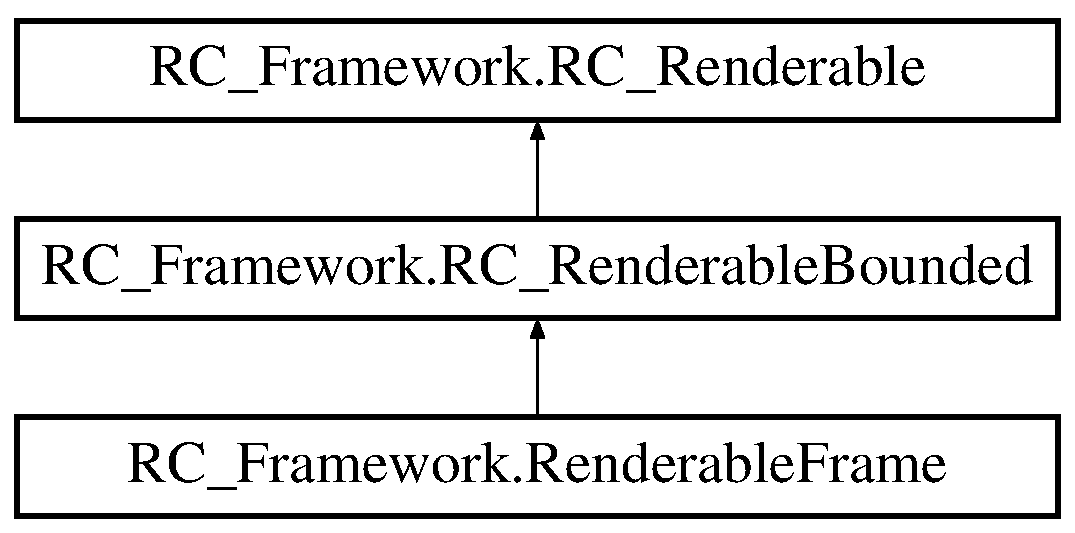
\includegraphics[height=3.000000cm]{class_r_c___framework_1_1_renderable_frame}
\end{center}
\end{figure}
\subsection*{Public Member Functions}
\begin{DoxyCompactItemize}
\item 
\mbox{\hyperlink{class_r_c___framework_1_1_renderable_frame_ac9e833096374af28d045ca825c8032f6}{Renderable\+Frame}} (\mbox{\hyperlink{class_r_c___framework_1_1_r_c___frame}{R\+C\+\_\+\+Frame}} frameZ, Rectangle destZ, Color colourZ)
\item 
\mbox{\hyperlink{class_r_c___framework_1_1_renderable_frame_abfdd49e56c1ac7f8e44c6977fe0cdcbe}{Renderable\+Frame}} (\mbox{\hyperlink{class_r_c___framework_1_1_r_c___frame}{R\+C\+\_\+\+Frame}} frameZ, Color colourZ, Graphics\+Device g)
\item 
override void \mbox{\hyperlink{class_r_c___framework_1_1_renderable_frame_af07cf299871051c7e1c6ca455ba1bab9}{Draw}} (Sprite\+Batch sb)
\begin{DoxyCompactList}\small\item\em Standard draw routine which assumes the renderable knows where it is \end{DoxyCompactList}\end{DoxyCompactItemize}
\subsection*{Additional Inherited Members}


\subsection{Detailed Description}
A renderable frame similar in most respects to the class \mbox{\hyperlink{class_r_c___framework_1_1_image_background}{Image\+Background}} 



\subsection{Constructor \& Destructor Documentation}
\mbox{\Hypertarget{class_r_c___framework_1_1_renderable_frame_ac9e833096374af28d045ca825c8032f6}\label{class_r_c___framework_1_1_renderable_frame_ac9e833096374af28d045ca825c8032f6}} 
\index{R\+C\+\_\+\+Framework\+::\+Renderable\+Frame@{R\+C\+\_\+\+Framework\+::\+Renderable\+Frame}!Renderable\+Frame@{Renderable\+Frame}}
\index{Renderable\+Frame@{Renderable\+Frame}!R\+C\+\_\+\+Framework\+::\+Renderable\+Frame@{R\+C\+\_\+\+Framework\+::\+Renderable\+Frame}}
\subsubsection{\texorpdfstring{Renderable\+Frame()}{RenderableFrame()}\hspace{0.1cm}{\footnotesize\ttfamily [1/2]}}
{\footnotesize\ttfamily R\+C\+\_\+\+Framework.\+Renderable\+Frame.\+Renderable\+Frame (\begin{DoxyParamCaption}\item[{\mbox{\hyperlink{class_r_c___framework_1_1_r_c___frame}{R\+C\+\_\+\+Frame}}}]{frameZ,  }\item[{Rectangle}]{destZ,  }\item[{Color}]{colourZ }\end{DoxyParamCaption})}

\mbox{\Hypertarget{class_r_c___framework_1_1_renderable_frame_abfdd49e56c1ac7f8e44c6977fe0cdcbe}\label{class_r_c___framework_1_1_renderable_frame_abfdd49e56c1ac7f8e44c6977fe0cdcbe}} 
\index{R\+C\+\_\+\+Framework\+::\+Renderable\+Frame@{R\+C\+\_\+\+Framework\+::\+Renderable\+Frame}!Renderable\+Frame@{Renderable\+Frame}}
\index{Renderable\+Frame@{Renderable\+Frame}!R\+C\+\_\+\+Framework\+::\+Renderable\+Frame@{R\+C\+\_\+\+Framework\+::\+Renderable\+Frame}}
\subsubsection{\texorpdfstring{Renderable\+Frame()}{RenderableFrame()}\hspace{0.1cm}{\footnotesize\ttfamily [2/2]}}
{\footnotesize\ttfamily R\+C\+\_\+\+Framework.\+Renderable\+Frame.\+Renderable\+Frame (\begin{DoxyParamCaption}\item[{\mbox{\hyperlink{class_r_c___framework_1_1_r_c___frame}{R\+C\+\_\+\+Frame}}}]{frameZ,  }\item[{Color}]{colourZ,  }\item[{Graphics\+Device}]{g }\end{DoxyParamCaption})}



\subsection{Member Function Documentation}
\mbox{\Hypertarget{class_r_c___framework_1_1_renderable_frame_af07cf299871051c7e1c6ca455ba1bab9}\label{class_r_c___framework_1_1_renderable_frame_af07cf299871051c7e1c6ca455ba1bab9}} 
\index{R\+C\+\_\+\+Framework\+::\+Renderable\+Frame@{R\+C\+\_\+\+Framework\+::\+Renderable\+Frame}!Draw@{Draw}}
\index{Draw@{Draw}!R\+C\+\_\+\+Framework\+::\+Renderable\+Frame@{R\+C\+\_\+\+Framework\+::\+Renderable\+Frame}}
\subsubsection{\texorpdfstring{Draw()}{Draw()}}
{\footnotesize\ttfamily override void R\+C\+\_\+\+Framework.\+Renderable\+Frame.\+Draw (\begin{DoxyParamCaption}\item[{Sprite\+Batch}]{sb }\end{DoxyParamCaption})\hspace{0.3cm}{\ttfamily [virtual]}}



Standard draw routine which assumes the renderable knows where it is 


\begin{DoxyParams}{Parameters}
{\em sb} & \\
\hline
\end{DoxyParams}


Reimplemented from \mbox{\hyperlink{class_r_c___framework_1_1_r_c___renderable_acc26db34e382a25a989c4c0dd0354b23}{R\+C\+\_\+\+Framework.\+R\+C\+\_\+\+Renderable}}.



The documentation for this class was generated from the following file\+:\begin{DoxyCompactItemize}
\item 
F\+:/\+B/\+R\+C\+\_\+\+Framework2018/\+Source/\mbox{\hyperlink{_r_c___frame_8cs}{R\+C\+\_\+\+Frame.\+cs}}\end{DoxyCompactItemize}

\hypertarget{class_r_c___framework_1_1_repeat_image}{}\section{R\+C\+\_\+\+Framework.\+Repeat\+Image Class Reference}
\label{class_r_c___framework_1_1_repeat_image}\index{R\+C\+\_\+\+Framework.\+Repeat\+Image@{R\+C\+\_\+\+Framework.\+Repeat\+Image}}


A List of images like a lives counter the destination rectange is the destination of just 1 image (the first image) If source is null then the whole image is used setting a background colour gives a background (helpfull for debugging) setting a gapgives you a gap  


Inheritance diagram for R\+C\+\_\+\+Framework.\+Repeat\+Image\+:\begin{figure}[H]
\begin{center}
\leavevmode
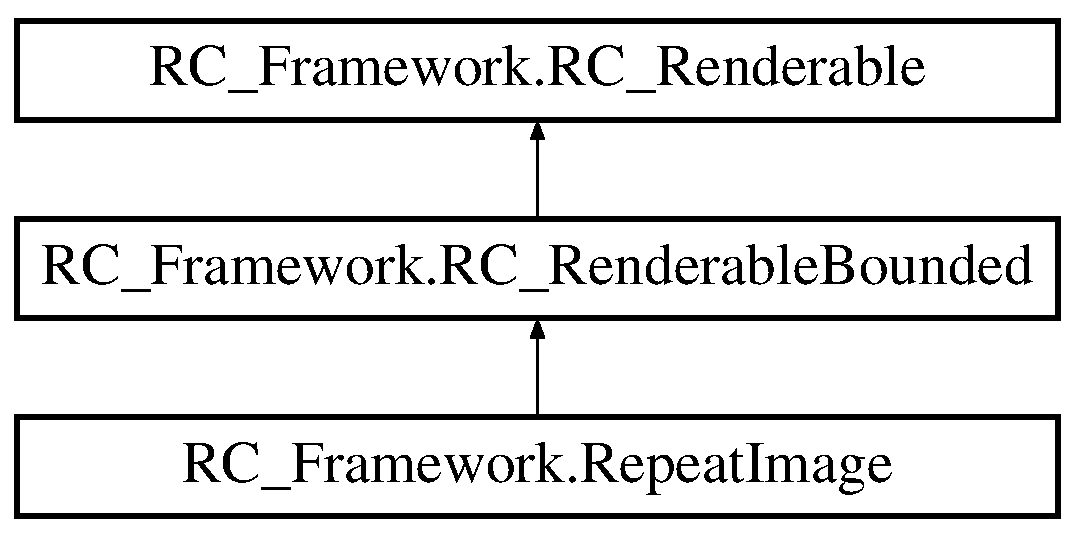
\includegraphics[height=3.000000cm]{class_r_c___framework_1_1_repeat_image}
\end{center}
\end{figure}
\subsection*{Public Member Functions}
\begin{DoxyCompactItemize}
\item 
\mbox{\hyperlink{class_r_c___framework_1_1_repeat_image_aaa671e1d98cedaf00dccb8b563b5dfc2}{Repeat\+Image}} (Texture2D texZ, Rectangle? sourceZ, Rectangle destZ, Color colourZ, int max\+NumberZ, int start\+Num)
\item 
int \mbox{\hyperlink{class_r_c___framework_1_1_repeat_image_ac3a04a412b50169bf9cb319d355d7afc}{add\+Num}} (int num\+To\+Add)
\item 
void \mbox{\hyperlink{class_r_c___framework_1_1_repeat_image_ab8d0d1a06f74b0a86c984a27a6902d04}{set\+Num}} (int num)
\item 
override void \mbox{\hyperlink{class_r_c___framework_1_1_repeat_image_ad0d9de5911c47f93d7ed1dc48f531283}{Draw}} (Sprite\+Batch sb)
\begin{DoxyCompactList}\small\item\em Standard draw routine which assumes the renderable knows where it is \end{DoxyCompactList}\end{DoxyCompactItemize}
\subsection*{Public Attributes}
\begin{DoxyCompactItemize}
\item 
Color \mbox{\hyperlink{class_r_c___framework_1_1_repeat_image_a37741513459c3910381e6574d2cc2132}{background\+Color}} = Color.\+Transparent
\item 
int \mbox{\hyperlink{class_r_c___framework_1_1_repeat_image_a6e4d724998e521f4af39bccfb036ffa6}{gap}} = 0
\end{DoxyCompactItemize}
\subsection*{Additional Inherited Members}


\subsection{Detailed Description}
A List of images like a lives counter the destination rectange is the destination of just 1 image (the first image) If source is null then the whole image is used setting a background colour gives a background (helpfull for debugging) setting a gapgives you a gap 



\subsection{Constructor \& Destructor Documentation}
\mbox{\Hypertarget{class_r_c___framework_1_1_repeat_image_aaa671e1d98cedaf00dccb8b563b5dfc2}\label{class_r_c___framework_1_1_repeat_image_aaa671e1d98cedaf00dccb8b563b5dfc2}} 
\index{R\+C\+\_\+\+Framework\+::\+Repeat\+Image@{R\+C\+\_\+\+Framework\+::\+Repeat\+Image}!Repeat\+Image@{Repeat\+Image}}
\index{Repeat\+Image@{Repeat\+Image}!R\+C\+\_\+\+Framework\+::\+Repeat\+Image@{R\+C\+\_\+\+Framework\+::\+Repeat\+Image}}
\subsubsection{\texorpdfstring{Repeat\+Image()}{RepeatImage()}}
{\footnotesize\ttfamily R\+C\+\_\+\+Framework.\+Repeat\+Image.\+Repeat\+Image (\begin{DoxyParamCaption}\item[{Texture2D}]{texZ,  }\item[{Rectangle?}]{sourceZ,  }\item[{Rectangle}]{destZ,  }\item[{Color}]{colourZ,  }\item[{int}]{max\+NumberZ,  }\item[{int}]{start\+Num }\end{DoxyParamCaption})}



\subsection{Member Function Documentation}
\mbox{\Hypertarget{class_r_c___framework_1_1_repeat_image_ac3a04a412b50169bf9cb319d355d7afc}\label{class_r_c___framework_1_1_repeat_image_ac3a04a412b50169bf9cb319d355d7afc}} 
\index{R\+C\+\_\+\+Framework\+::\+Repeat\+Image@{R\+C\+\_\+\+Framework\+::\+Repeat\+Image}!add\+Num@{add\+Num}}
\index{add\+Num@{add\+Num}!R\+C\+\_\+\+Framework\+::\+Repeat\+Image@{R\+C\+\_\+\+Framework\+::\+Repeat\+Image}}
\subsubsection{\texorpdfstring{add\+Num()}{addNum()}}
{\footnotesize\ttfamily int R\+C\+\_\+\+Framework.\+Repeat\+Image.\+add\+Num (\begin{DoxyParamCaption}\item[{int}]{num\+To\+Add }\end{DoxyParamCaption})}

\mbox{\Hypertarget{class_r_c___framework_1_1_repeat_image_ad0d9de5911c47f93d7ed1dc48f531283}\label{class_r_c___framework_1_1_repeat_image_ad0d9de5911c47f93d7ed1dc48f531283}} 
\index{R\+C\+\_\+\+Framework\+::\+Repeat\+Image@{R\+C\+\_\+\+Framework\+::\+Repeat\+Image}!Draw@{Draw}}
\index{Draw@{Draw}!R\+C\+\_\+\+Framework\+::\+Repeat\+Image@{R\+C\+\_\+\+Framework\+::\+Repeat\+Image}}
\subsubsection{\texorpdfstring{Draw()}{Draw()}}
{\footnotesize\ttfamily override void R\+C\+\_\+\+Framework.\+Repeat\+Image.\+Draw (\begin{DoxyParamCaption}\item[{Sprite\+Batch}]{sb }\end{DoxyParamCaption})\hspace{0.3cm}{\ttfamily [virtual]}}



Standard draw routine which assumes the renderable knows where it is 


\begin{DoxyParams}{Parameters}
{\em sb} & \\
\hline
\end{DoxyParams}


Reimplemented from \mbox{\hyperlink{class_r_c___framework_1_1_r_c___renderable_acc26db34e382a25a989c4c0dd0354b23}{R\+C\+\_\+\+Framework.\+R\+C\+\_\+\+Renderable}}.

\mbox{\Hypertarget{class_r_c___framework_1_1_repeat_image_ab8d0d1a06f74b0a86c984a27a6902d04}\label{class_r_c___framework_1_1_repeat_image_ab8d0d1a06f74b0a86c984a27a6902d04}} 
\index{R\+C\+\_\+\+Framework\+::\+Repeat\+Image@{R\+C\+\_\+\+Framework\+::\+Repeat\+Image}!set\+Num@{set\+Num}}
\index{set\+Num@{set\+Num}!R\+C\+\_\+\+Framework\+::\+Repeat\+Image@{R\+C\+\_\+\+Framework\+::\+Repeat\+Image}}
\subsubsection{\texorpdfstring{set\+Num()}{setNum()}}
{\footnotesize\ttfamily void R\+C\+\_\+\+Framework.\+Repeat\+Image.\+set\+Num (\begin{DoxyParamCaption}\item[{int}]{num }\end{DoxyParamCaption})}



\subsection{Member Data Documentation}
\mbox{\Hypertarget{class_r_c___framework_1_1_repeat_image_a37741513459c3910381e6574d2cc2132}\label{class_r_c___framework_1_1_repeat_image_a37741513459c3910381e6574d2cc2132}} 
\index{R\+C\+\_\+\+Framework\+::\+Repeat\+Image@{R\+C\+\_\+\+Framework\+::\+Repeat\+Image}!background\+Color@{background\+Color}}
\index{background\+Color@{background\+Color}!R\+C\+\_\+\+Framework\+::\+Repeat\+Image@{R\+C\+\_\+\+Framework\+::\+Repeat\+Image}}
\subsubsection{\texorpdfstring{background\+Color}{backgroundColor}}
{\footnotesize\ttfamily Color R\+C\+\_\+\+Framework.\+Repeat\+Image.\+background\+Color = Color.\+Transparent}

\mbox{\Hypertarget{class_r_c___framework_1_1_repeat_image_a6e4d724998e521f4af39bccfb036ffa6}\label{class_r_c___framework_1_1_repeat_image_a6e4d724998e521f4af39bccfb036ffa6}} 
\index{R\+C\+\_\+\+Framework\+::\+Repeat\+Image@{R\+C\+\_\+\+Framework\+::\+Repeat\+Image}!gap@{gap}}
\index{gap@{gap}!R\+C\+\_\+\+Framework\+::\+Repeat\+Image@{R\+C\+\_\+\+Framework\+::\+Repeat\+Image}}
\subsubsection{\texorpdfstring{gap}{gap}}
{\footnotesize\ttfamily int R\+C\+\_\+\+Framework.\+Repeat\+Image.\+gap = 0}



The documentation for this class was generated from the following file\+:\begin{DoxyCompactItemize}
\item 
F\+:/\+B/\+R\+C\+\_\+\+Framework2018/\+Source/\mbox{\hyperlink{_r_c___renderable_bounded_8cs}{R\+C\+\_\+\+Renderable\+Bounded.\+cs}}\end{DoxyCompactItemize}

\hypertarget{class_r_c___framework_1_1_scroll_back_ground}{}\section{R\+C\+\_\+\+Framework.\+Scroll\+Back\+Ground Class Reference}
\label{class_r_c___framework_1_1_scroll_back_ground}\index{R\+C\+\_\+\+Framework.\+Scroll\+Back\+Ground@{R\+C\+\_\+\+Framework.\+Scroll\+Back\+Ground}}


Scrolling background Horizontal or vertical but not both  


Inheritance diagram for R\+C\+\_\+\+Framework.\+Scroll\+Back\+Ground\+:\begin{figure}[H]
\begin{center}
\leavevmode
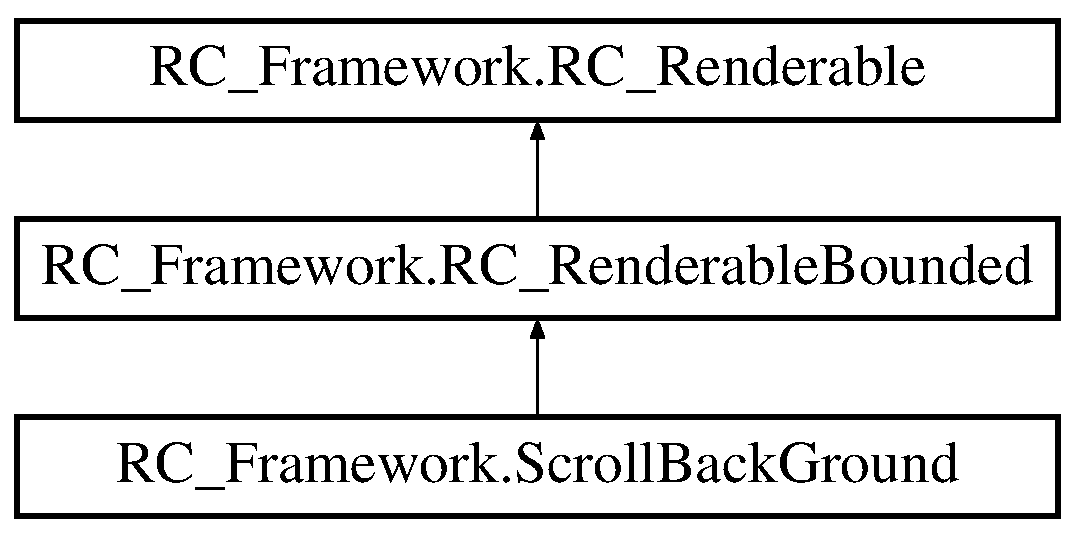
\includegraphics[height=3.000000cm]{class_r_c___framework_1_1_scroll_back_ground}
\end{center}
\end{figure}
\subsection*{Public Member Functions}
\begin{DoxyCompactItemize}
\item 
\mbox{\hyperlink{class_r_c___framework_1_1_scroll_back_ground_aa7ce7d0dc4170243b94f399854918ab0}{Scroll\+Back\+Ground}} (Rectangle boundsZ)
\item 
\mbox{\hyperlink{class_r_c___framework_1_1_scroll_back_ground_added00d79c976a3e1bf2a90ff1e62666}{Scroll\+Back\+Ground}} (Texture2D texZ, Rectangle source, Rectangle dest, float delta, int directionZ)
\begin{DoxyCompactList}\small\item\em direction 0=none 1=vertical 2=horizontal \end{DoxyCompactList}\item 
void \mbox{\hyperlink{class_r_c___framework_1_1_scroll_back_ground_a51b38c4f29b384ab4421e420b3fd7201}{set\+Scroll\+Speed}} (float speed)
\item 
override void \mbox{\hyperlink{class_r_c___framework_1_1_scroll_back_ground_a7b9513679627c90648d41b952d4231d1}{Draw}} (Sprite\+Batch sb)
\begin{DoxyCompactList}\small\item\em Standard draw routine which assumes the renderable knows where it is \end{DoxyCompactList}\item 
override void \mbox{\hyperlink{class_r_c___framework_1_1_scroll_back_ground_ac999fc666d1abebe93d7d659e5a53e8a}{Update}} (Game\+Time game\+Time)
\item 
override void \mbox{\hyperlink{class_r_c___framework_1_1_scroll_back_ground_aeb2e92fd02bce76a76d4002aa94ff3d5}{reset}} ()
\end{DoxyCompactItemize}
\subsection*{Additional Inherited Members}


\subsection{Detailed Description}
Scrolling background Horizontal or vertical but not both 



\subsection{Constructor \& Destructor Documentation}
\mbox{\Hypertarget{class_r_c___framework_1_1_scroll_back_ground_aa7ce7d0dc4170243b94f399854918ab0}\label{class_r_c___framework_1_1_scroll_back_ground_aa7ce7d0dc4170243b94f399854918ab0}} 
\index{R\+C\+\_\+\+Framework\+::\+Scroll\+Back\+Ground@{R\+C\+\_\+\+Framework\+::\+Scroll\+Back\+Ground}!Scroll\+Back\+Ground@{Scroll\+Back\+Ground}}
\index{Scroll\+Back\+Ground@{Scroll\+Back\+Ground}!R\+C\+\_\+\+Framework\+::\+Scroll\+Back\+Ground@{R\+C\+\_\+\+Framework\+::\+Scroll\+Back\+Ground}}
\subsubsection{\texorpdfstring{Scroll\+Back\+Ground()}{ScrollBackGround()}\hspace{0.1cm}{\footnotesize\ttfamily [1/2]}}
{\footnotesize\ttfamily R\+C\+\_\+\+Framework.\+Scroll\+Back\+Ground.\+Scroll\+Back\+Ground (\begin{DoxyParamCaption}\item[{Rectangle}]{boundsZ }\end{DoxyParamCaption})}

\mbox{\Hypertarget{class_r_c___framework_1_1_scroll_back_ground_added00d79c976a3e1bf2a90ff1e62666}\label{class_r_c___framework_1_1_scroll_back_ground_added00d79c976a3e1bf2a90ff1e62666}} 
\index{R\+C\+\_\+\+Framework\+::\+Scroll\+Back\+Ground@{R\+C\+\_\+\+Framework\+::\+Scroll\+Back\+Ground}!Scroll\+Back\+Ground@{Scroll\+Back\+Ground}}
\index{Scroll\+Back\+Ground@{Scroll\+Back\+Ground}!R\+C\+\_\+\+Framework\+::\+Scroll\+Back\+Ground@{R\+C\+\_\+\+Framework\+::\+Scroll\+Back\+Ground}}
\subsubsection{\texorpdfstring{Scroll\+Back\+Ground()}{ScrollBackGround()}\hspace{0.1cm}{\footnotesize\ttfamily [2/2]}}
{\footnotesize\ttfamily R\+C\+\_\+\+Framework.\+Scroll\+Back\+Ground.\+Scroll\+Back\+Ground (\begin{DoxyParamCaption}\item[{Texture2D}]{texZ,  }\item[{Rectangle}]{source,  }\item[{Rectangle}]{dest,  }\item[{float}]{delta,  }\item[{int}]{directionZ }\end{DoxyParamCaption})}



direction 0=none 1=vertical 2=horizontal 


\begin{DoxyParams}{Parameters}
{\em texZ} & \\
\hline
{\em source} & \\
\hline
{\em dest} & \\
\hline
{\em delta} & \\
\hline
{\em directionZ} & \\
\hline
\end{DoxyParams}


\subsection{Member Function Documentation}
\mbox{\Hypertarget{class_r_c___framework_1_1_scroll_back_ground_a7b9513679627c90648d41b952d4231d1}\label{class_r_c___framework_1_1_scroll_back_ground_a7b9513679627c90648d41b952d4231d1}} 
\index{R\+C\+\_\+\+Framework\+::\+Scroll\+Back\+Ground@{R\+C\+\_\+\+Framework\+::\+Scroll\+Back\+Ground}!Draw@{Draw}}
\index{Draw@{Draw}!R\+C\+\_\+\+Framework\+::\+Scroll\+Back\+Ground@{R\+C\+\_\+\+Framework\+::\+Scroll\+Back\+Ground}}
\subsubsection{\texorpdfstring{Draw()}{Draw()}}
{\footnotesize\ttfamily override void R\+C\+\_\+\+Framework.\+Scroll\+Back\+Ground.\+Draw (\begin{DoxyParamCaption}\item[{Sprite\+Batch}]{sb }\end{DoxyParamCaption})\hspace{0.3cm}{\ttfamily [virtual]}}



Standard draw routine which assumes the renderable knows where it is 


\begin{DoxyParams}{Parameters}
{\em sb} & \\
\hline
\end{DoxyParams}


Reimplemented from \mbox{\hyperlink{class_r_c___framework_1_1_r_c___renderable_acc26db34e382a25a989c4c0dd0354b23}{R\+C\+\_\+\+Framework.\+R\+C\+\_\+\+Renderable}}.

\mbox{\Hypertarget{class_r_c___framework_1_1_scroll_back_ground_aeb2e92fd02bce76a76d4002aa94ff3d5}\label{class_r_c___framework_1_1_scroll_back_ground_aeb2e92fd02bce76a76d4002aa94ff3d5}} 
\index{R\+C\+\_\+\+Framework\+::\+Scroll\+Back\+Ground@{R\+C\+\_\+\+Framework\+::\+Scroll\+Back\+Ground}!reset@{reset}}
\index{reset@{reset}!R\+C\+\_\+\+Framework\+::\+Scroll\+Back\+Ground@{R\+C\+\_\+\+Framework\+::\+Scroll\+Back\+Ground}}
\subsubsection{\texorpdfstring{reset()}{reset()}}
{\footnotesize\ttfamily override void R\+C\+\_\+\+Framework.\+Scroll\+Back\+Ground.\+reset (\begin{DoxyParamCaption}{ }\end{DoxyParamCaption})\hspace{0.3cm}{\ttfamily [virtual]}}



Reimplemented from \mbox{\hyperlink{class_r_c___framework_1_1_r_c___renderable_ae65ce69704d15963789f421b58618b1f}{R\+C\+\_\+\+Framework.\+R\+C\+\_\+\+Renderable}}.

\mbox{\Hypertarget{class_r_c___framework_1_1_scroll_back_ground_a51b38c4f29b384ab4421e420b3fd7201}\label{class_r_c___framework_1_1_scroll_back_ground_a51b38c4f29b384ab4421e420b3fd7201}} 
\index{R\+C\+\_\+\+Framework\+::\+Scroll\+Back\+Ground@{R\+C\+\_\+\+Framework\+::\+Scroll\+Back\+Ground}!set\+Scroll\+Speed@{set\+Scroll\+Speed}}
\index{set\+Scroll\+Speed@{set\+Scroll\+Speed}!R\+C\+\_\+\+Framework\+::\+Scroll\+Back\+Ground@{R\+C\+\_\+\+Framework\+::\+Scroll\+Back\+Ground}}
\subsubsection{\texorpdfstring{set\+Scroll\+Speed()}{setScrollSpeed()}}
{\footnotesize\ttfamily void R\+C\+\_\+\+Framework.\+Scroll\+Back\+Ground.\+set\+Scroll\+Speed (\begin{DoxyParamCaption}\item[{float}]{speed }\end{DoxyParamCaption})}

\mbox{\Hypertarget{class_r_c___framework_1_1_scroll_back_ground_ac999fc666d1abebe93d7d659e5a53e8a}\label{class_r_c___framework_1_1_scroll_back_ground_ac999fc666d1abebe93d7d659e5a53e8a}} 
\index{R\+C\+\_\+\+Framework\+::\+Scroll\+Back\+Ground@{R\+C\+\_\+\+Framework\+::\+Scroll\+Back\+Ground}!Update@{Update}}
\index{Update@{Update}!R\+C\+\_\+\+Framework\+::\+Scroll\+Back\+Ground@{R\+C\+\_\+\+Framework\+::\+Scroll\+Back\+Ground}}
\subsubsection{\texorpdfstring{Update()}{Update()}}
{\footnotesize\ttfamily override void R\+C\+\_\+\+Framework.\+Scroll\+Back\+Ground.\+Update (\begin{DoxyParamCaption}\item[{Game\+Time}]{game\+Time }\end{DoxyParamCaption})\hspace{0.3cm}{\ttfamily [virtual]}}



Reimplemented from \mbox{\hyperlink{class_r_c___framework_1_1_r_c___renderable_a5745bedc7ba0587aa1e1d8563c357228}{R\+C\+\_\+\+Framework.\+R\+C\+\_\+\+Renderable}}.



The documentation for this class was generated from the following file\+:\begin{DoxyCompactItemize}
\item 
F\+:/\+B/\+R\+C\+\_\+\+Framework2018/\+Source/\mbox{\hyperlink{_r_c___renderable_bounded_8cs}{R\+C\+\_\+\+Renderable\+Bounded.\+cs}}\end{DoxyCompactItemize}

\hypertarget{class_r_c___framework_1_1_silly_font}{}\section{R\+C\+\_\+\+Framework.\+Silly\+Font Class Reference}
\label{class_r_c___framework_1_1_silly_font}\index{R\+C\+\_\+\+Framework.\+Silly\+Font@{R\+C\+\_\+\+Framework.\+Silly\+Font}}


Ok a low quality 8x8 font which is defined in code very handy for debugging and resizing, but not really of comercial quality  


Inheritance diagram for R\+C\+\_\+\+Framework.\+Silly\+Font\+:\begin{figure}[H]
\begin{center}
\leavevmode
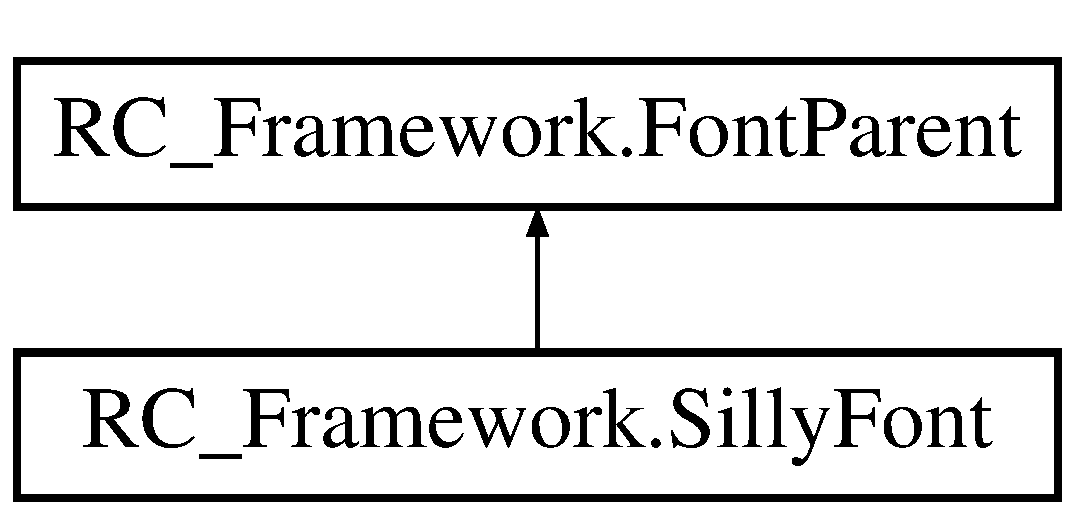
\includegraphics[height=2.000000cm]{class_r_c___framework_1_1_silly_font}
\end{center}
\end{figure}
\subsection*{Public Member Functions}
\begin{DoxyCompactItemize}
\item 
\mbox{\hyperlink{class_r_c___framework_1_1_silly_font_a72496d4a4a8b21d77edcf2c1b50587cb}{Silly\+Font}} (Graphics\+Device g\+Device, Color back\+Ground\+Color, Color foreground\+Color)
\end{DoxyCompactItemize}
\subsection*{Public Attributes}
\begin{DoxyCompactItemize}
\item 
\mbox{\hyperlink{class_r_c___framework_1_1_r_c___surface}{R\+C\+\_\+\+Surface}} \mbox{[}$\,$\mbox{]} \mbox{\hyperlink{class_r_c___framework_1_1_silly_font_a9537d47e675c0bc00bdd024666afeb9f}{fnt}} =null
\end{DoxyCompactItemize}
\subsection*{Static Public Attributes}
\begin{DoxyCompactItemize}
\item 
static Color \mbox{[}$\,$\mbox{]} \mbox{\hyperlink{class_r_c___framework_1_1_silly_font_acc43dfc99e4db0923967255bb1fbd02f}{Pallete11}}
\item 
static String \mbox{\hyperlink{class_r_c___framework_1_1_silly_font_a3ee61138b396e76502ed9783517712c5}{Pal11}}
\end{DoxyCompactItemize}


\subsection{Detailed Description}
Ok a low quality 8x8 font which is defined in code very handy for debugging and resizing, but not really of comercial quality 



\subsection{Constructor \& Destructor Documentation}
\mbox{\Hypertarget{class_r_c___framework_1_1_silly_font_a72496d4a4a8b21d77edcf2c1b50587cb}\label{class_r_c___framework_1_1_silly_font_a72496d4a4a8b21d77edcf2c1b50587cb}} 
\index{R\+C\+\_\+\+Framework\+::\+Silly\+Font@{R\+C\+\_\+\+Framework\+::\+Silly\+Font}!Silly\+Font@{Silly\+Font}}
\index{Silly\+Font@{Silly\+Font}!R\+C\+\_\+\+Framework\+::\+Silly\+Font@{R\+C\+\_\+\+Framework\+::\+Silly\+Font}}
\subsubsection{\texorpdfstring{Silly\+Font()}{SillyFont()}}
{\footnotesize\ttfamily R\+C\+\_\+\+Framework.\+Silly\+Font.\+Silly\+Font (\begin{DoxyParamCaption}\item[{Graphics\+Device}]{g\+Device,  }\item[{Color}]{back\+Ground\+Color,  }\item[{Color}]{foreground\+Color }\end{DoxyParamCaption})}



\subsection{Member Data Documentation}
\mbox{\Hypertarget{class_r_c___framework_1_1_silly_font_a9537d47e675c0bc00bdd024666afeb9f}\label{class_r_c___framework_1_1_silly_font_a9537d47e675c0bc00bdd024666afeb9f}} 
\index{R\+C\+\_\+\+Framework\+::\+Silly\+Font@{R\+C\+\_\+\+Framework\+::\+Silly\+Font}!fnt@{fnt}}
\index{fnt@{fnt}!R\+C\+\_\+\+Framework\+::\+Silly\+Font@{R\+C\+\_\+\+Framework\+::\+Silly\+Font}}
\subsubsection{\texorpdfstring{fnt}{fnt}}
{\footnotesize\ttfamily \mbox{\hyperlink{class_r_c___framework_1_1_r_c___surface}{R\+C\+\_\+\+Surface}} \mbox{[}$\,$\mbox{]} R\+C\+\_\+\+Framework.\+Silly\+Font.\+fnt =null}

\mbox{\Hypertarget{class_r_c___framework_1_1_silly_font_a3ee61138b396e76502ed9783517712c5}\label{class_r_c___framework_1_1_silly_font_a3ee61138b396e76502ed9783517712c5}} 
\index{R\+C\+\_\+\+Framework\+::\+Silly\+Font@{R\+C\+\_\+\+Framework\+::\+Silly\+Font}!Pal11@{Pal11}}
\index{Pal11@{Pal11}!R\+C\+\_\+\+Framework\+::\+Silly\+Font@{R\+C\+\_\+\+Framework\+::\+Silly\+Font}}
\subsubsection{\texorpdfstring{Pal11}{Pal11}}
{\footnotesize\ttfamily String R\+C\+\_\+\+Framework.\+Silly\+Font.\+Pal11\hspace{0.3cm}{\ttfamily [static]}}

\mbox{\Hypertarget{class_r_c___framework_1_1_silly_font_acc43dfc99e4db0923967255bb1fbd02f}\label{class_r_c___framework_1_1_silly_font_acc43dfc99e4db0923967255bb1fbd02f}} 
\index{R\+C\+\_\+\+Framework\+::\+Silly\+Font@{R\+C\+\_\+\+Framework\+::\+Silly\+Font}!Pallete11@{Pallete11}}
\index{Pallete11@{Pallete11}!R\+C\+\_\+\+Framework\+::\+Silly\+Font@{R\+C\+\_\+\+Framework\+::\+Silly\+Font}}
\subsubsection{\texorpdfstring{Pallete11}{Pallete11}}
{\footnotesize\ttfamily Color \mbox{[}$\,$\mbox{]} R\+C\+\_\+\+Framework.\+Silly\+Font.\+Pallete11\hspace{0.3cm}{\ttfamily [static]}}



The documentation for this class was generated from the following file\+:\begin{DoxyCompactItemize}
\item 
F\+:/\+B/\+R\+C\+\_\+\+Framework2018/\+Source/\mbox{\hyperlink{_r_c___util_text_8cs}{R\+C\+\_\+\+Util\+Text.\+cs}}\end{DoxyCompactItemize}

\hypertarget{class_r_c___framework_1_1_silly_font16}{}\section{R\+C\+\_\+\+Framework.\+Silly\+Font16 Class Reference}
\label{class_r_c___framework_1_1_silly_font16}\index{R\+C\+\_\+\+Framework.\+Silly\+Font16@{R\+C\+\_\+\+Framework.\+Silly\+Font16}}


Simply the 8by8 font doubled in size -\/ it tends to blur less when resized  


Inheritance diagram for R\+C\+\_\+\+Framework.\+Silly\+Font16\+:\begin{figure}[H]
\begin{center}
\leavevmode
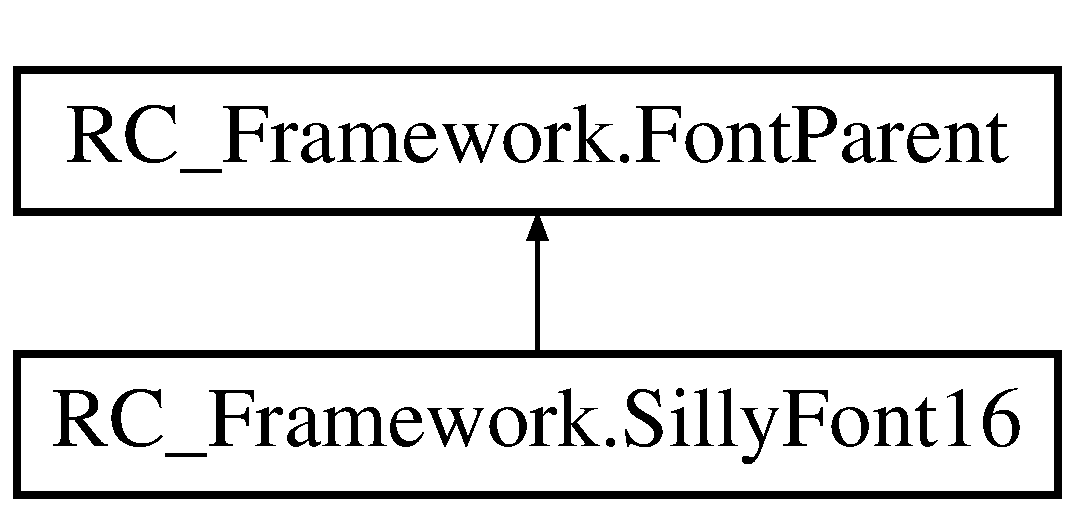
\includegraphics[height=2.000000cm]{class_r_c___framework_1_1_silly_font16}
\end{center}
\end{figure}
\subsection*{Public Member Functions}
\begin{DoxyCompactItemize}
\item 
override int \mbox{\hyperlink{class_r_c___framework_1_1_silly_font16_aa718495839a1492ebf5d7245d7d4620a}{charwidth}} ()
\item 
\mbox{\hyperlink{class_r_c___framework_1_1_silly_font16_aac4f3796b62deae3675e85c90b44363d}{Silly\+Font16}} (Graphics\+Device g\+Device, Color back\+Ground\+Color, Color foreground\+Color)
\end{DoxyCompactItemize}
\subsection*{Additional Inherited Members}


\subsection{Detailed Description}
Simply the 8by8 font doubled in size -\/ it tends to blur less when resized 



\subsection{Constructor \& Destructor Documentation}
\mbox{\Hypertarget{class_r_c___framework_1_1_silly_font16_aac4f3796b62deae3675e85c90b44363d}\label{class_r_c___framework_1_1_silly_font16_aac4f3796b62deae3675e85c90b44363d}} 
\index{R\+C\+\_\+\+Framework\+::\+Silly\+Font16@{R\+C\+\_\+\+Framework\+::\+Silly\+Font16}!Silly\+Font16@{Silly\+Font16}}
\index{Silly\+Font16@{Silly\+Font16}!R\+C\+\_\+\+Framework\+::\+Silly\+Font16@{R\+C\+\_\+\+Framework\+::\+Silly\+Font16}}
\subsubsection{\texorpdfstring{Silly\+Font16()}{SillyFont16()}}
{\footnotesize\ttfamily R\+C\+\_\+\+Framework.\+Silly\+Font16.\+Silly\+Font16 (\begin{DoxyParamCaption}\item[{Graphics\+Device}]{g\+Device,  }\item[{Color}]{back\+Ground\+Color,  }\item[{Color}]{foreground\+Color }\end{DoxyParamCaption})}



\subsection{Member Function Documentation}
\mbox{\Hypertarget{class_r_c___framework_1_1_silly_font16_aa718495839a1492ebf5d7245d7d4620a}\label{class_r_c___framework_1_1_silly_font16_aa718495839a1492ebf5d7245d7d4620a}} 
\index{R\+C\+\_\+\+Framework\+::\+Silly\+Font16@{R\+C\+\_\+\+Framework\+::\+Silly\+Font16}!charwidth@{charwidth}}
\index{charwidth@{charwidth}!R\+C\+\_\+\+Framework\+::\+Silly\+Font16@{R\+C\+\_\+\+Framework\+::\+Silly\+Font16}}
\subsubsection{\texorpdfstring{charwidth()}{charwidth()}}
{\footnotesize\ttfamily override int R\+C\+\_\+\+Framework.\+Silly\+Font16.\+charwidth (\begin{DoxyParamCaption}{ }\end{DoxyParamCaption})\hspace{0.3cm}{\ttfamily [virtual]}}



Reimplemented from \mbox{\hyperlink{class_r_c___framework_1_1_font_parent_af32d5427b8feea59eb6f303ac3c36516}{R\+C\+\_\+\+Framework.\+Font\+Parent}}.



The documentation for this class was generated from the following file\+:\begin{DoxyCompactItemize}
\item 
F\+:/\+B/\+R\+C\+\_\+\+Framework2018/\+Source/\mbox{\hyperlink{_r_c___util_text_8cs}{R\+C\+\_\+\+Util\+Text.\+cs}}\end{DoxyCompactItemize}

\hypertarget{class_r_c___framework_1_1_simple_sprite_factory}{}\section{R\+C\+\_\+\+Framework.\+Simple\+Sprite\+Factory Class Reference}
\label{class_r_c___framework_1_1_simple_sprite_factory}\index{R\+C\+\_\+\+Framework.\+Simple\+Sprite\+Factory@{R\+C\+\_\+\+Framework.\+Simple\+Sprite\+Factory}}


This is a simple class that creates sprites based on a position factory  


Inheritance diagram for R\+C\+\_\+\+Framework.\+Simple\+Sprite\+Factory\+:\begin{figure}[H]
\begin{center}
\leavevmode
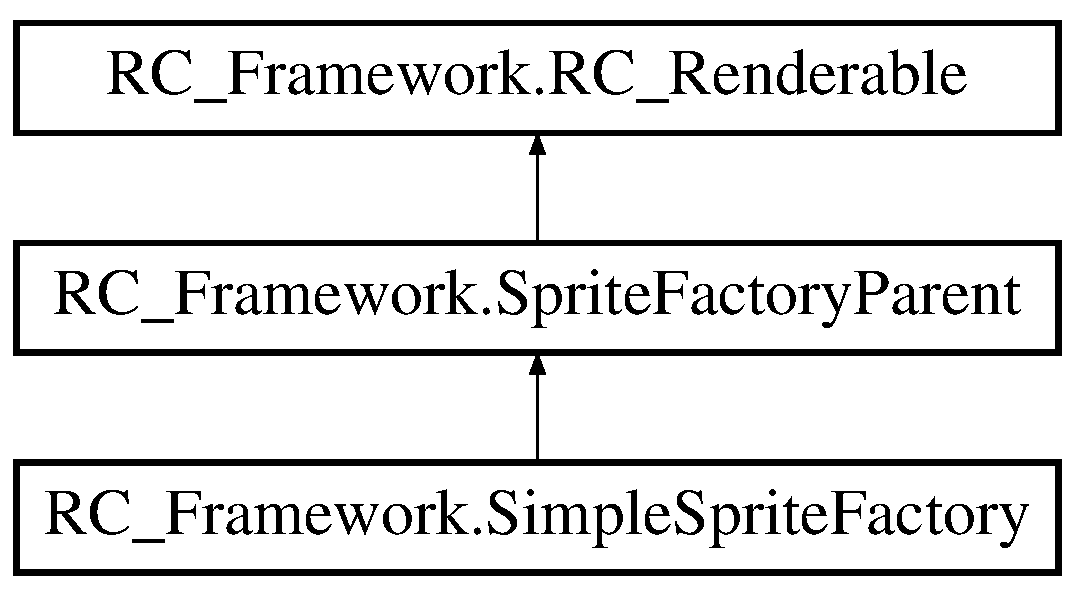
\includegraphics[height=3.000000cm]{class_r_c___framework_1_1_simple_sprite_factory}
\end{center}
\end{figure}
\subsection*{Public Member Functions}
\begin{DoxyCompactItemize}
\item 
\mbox{\hyperlink{class_r_c___framework_1_1_simple_sprite_factory_ad978a3be1e1b931e9ce3f617d95b79bb}{Simple\+Sprite\+Factory}} (Texture2D texQ, \mbox{\hyperlink{class_r_c___framework_1_1_r_c___position_factory}{R\+C\+\_\+\+Position\+Factory}} pos\+FactoryQ, float widthQ, float heightQ)
\item 
override \mbox{\hyperlink{class_r_c___framework_1_1_sprite3}{Sprite3}} \mbox{\hyperlink{class_r_c___framework_1_1_simple_sprite_factory_ab008431fcc3f967b70de9a155d1a529a}{generate\+At}} (int kind, int param, Rectangle boundz)
\begin{DoxyCompactList}\small\item\em generate sprite with all parametrs \end{DoxyCompactList}\end{DoxyCompactItemize}
\subsection*{Additional Inherited Members}


\subsection{Detailed Description}
This is a simple class that creates sprites based on a position factory 

\subsection{Constructor \& Destructor Documentation}
\mbox{\Hypertarget{class_r_c___framework_1_1_simple_sprite_factory_ad978a3be1e1b931e9ce3f617d95b79bb}\label{class_r_c___framework_1_1_simple_sprite_factory_ad978a3be1e1b931e9ce3f617d95b79bb}} 
\index{R\+C\+\_\+\+Framework\+::\+Simple\+Sprite\+Factory@{R\+C\+\_\+\+Framework\+::\+Simple\+Sprite\+Factory}!Simple\+Sprite\+Factory@{Simple\+Sprite\+Factory}}
\index{Simple\+Sprite\+Factory@{Simple\+Sprite\+Factory}!R\+C\+\_\+\+Framework\+::\+Simple\+Sprite\+Factory@{R\+C\+\_\+\+Framework\+::\+Simple\+Sprite\+Factory}}
\subsubsection{\texorpdfstring{Simple\+Sprite\+Factory()}{SimpleSpriteFactory()}}
{\footnotesize\ttfamily R\+C\+\_\+\+Framework.\+Simple\+Sprite\+Factory.\+Simple\+Sprite\+Factory (\begin{DoxyParamCaption}\item[{Texture2D}]{texQ,  }\item[{\mbox{\hyperlink{class_r_c___framework_1_1_r_c___position_factory}{R\+C\+\_\+\+Position\+Factory}}}]{pos\+FactoryQ,  }\item[{float}]{widthQ,  }\item[{float}]{heightQ }\end{DoxyParamCaption})}



\subsection{Member Function Documentation}
\mbox{\Hypertarget{class_r_c___framework_1_1_simple_sprite_factory_ab008431fcc3f967b70de9a155d1a529a}\label{class_r_c___framework_1_1_simple_sprite_factory_ab008431fcc3f967b70de9a155d1a529a}} 
\index{R\+C\+\_\+\+Framework\+::\+Simple\+Sprite\+Factory@{R\+C\+\_\+\+Framework\+::\+Simple\+Sprite\+Factory}!generate\+At@{generate\+At}}
\index{generate\+At@{generate\+At}!R\+C\+\_\+\+Framework\+::\+Simple\+Sprite\+Factory@{R\+C\+\_\+\+Framework\+::\+Simple\+Sprite\+Factory}}
\subsubsection{\texorpdfstring{generate\+At()}{generateAt()}}
{\footnotesize\ttfamily override \mbox{\hyperlink{class_r_c___framework_1_1_sprite3}{Sprite3}} R\+C\+\_\+\+Framework.\+Simple\+Sprite\+Factory.\+generate\+At (\begin{DoxyParamCaption}\item[{int}]{kind,  }\item[{int}]{param,  }\item[{Rectangle}]{boundz }\end{DoxyParamCaption})\hspace{0.3cm}{\ttfamily [virtual]}}



generate sprite with all parametrs 


\begin{DoxyParams}{Parameters}
{\em x} & \\
\hline
{\em y} & \\
\hline
{\em width} & \\
\hline
{\em heigth} & \\
\hline
\end{DoxyParams}
\begin{DoxyReturn}{Returns}

\end{DoxyReturn}


Implements \mbox{\hyperlink{class_r_c___framework_1_1_sprite_factory_parent_ace3d0e7a00dd88a16a652ed5fa6a90bd}{R\+C\+\_\+\+Framework.\+Sprite\+Factory\+Parent}}.



The documentation for this class was generated from the following file\+:\begin{DoxyCompactItemize}
\item 
F\+:/\+B/\+R\+C\+\_\+\+Framework2018/\+Source/\mbox{\hyperlink{_r_c___sprite3_8cs}{R\+C\+\_\+\+Sprite3.\+cs}}\end{DoxyCompactItemize}

\hypertarget{class_r_c___framework_1_1_sprite12_step}{}\section{R\+C\+\_\+\+Framework.\+Sprite12\+Step Class Reference}
\label{class_r_c___framework_1_1_sprite12_step}\index{R\+C\+\_\+\+Framework.\+Sprite12\+Step@{R\+C\+\_\+\+Framework.\+Sprite12\+Step}}
Inheritance diagram for R\+C\+\_\+\+Framework.\+Sprite12\+Step\+:\begin{figure}[H]
\begin{center}
\leavevmode
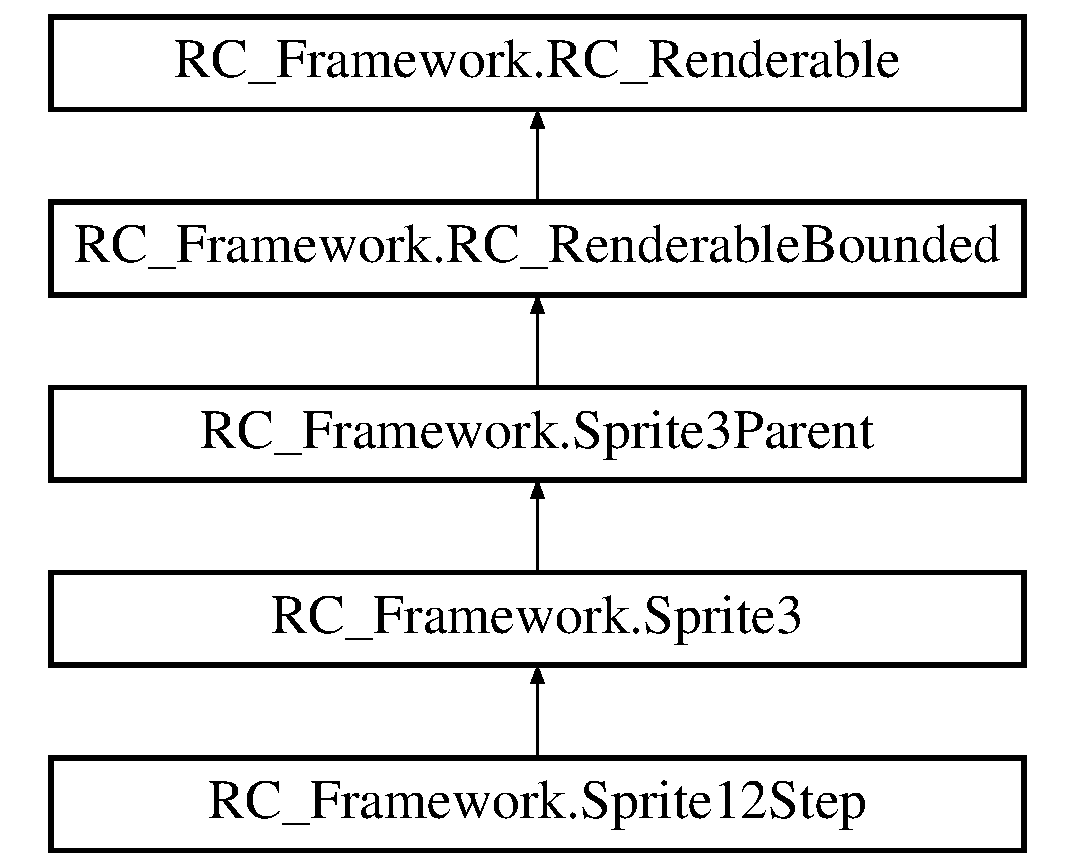
\includegraphics[height=5.000000cm]{class_r_c___framework_1_1_sprite12_step}
\end{center}
\end{figure}
\subsection*{Public Member Functions}
\begin{DoxyCompactItemize}
\item 
\mbox{\hyperlink{class_r_c___framework_1_1_sprite12_step_aed9fb46b122f42a6291527345d7fe390}{Sprite12\+Step}} (bool visibleZ, Texture2D texZ, float x, float y, int xsize, int ysize, int dir\+Anim\+Init)
\item 
void \mbox{\hyperlink{class_r_c___framework_1_1_sprite12_step_acb271325836aa42c56e60f8093eaa207}{set\+H\+S\+Bottom}} ()
\begin{DoxyCompactList}\small\item\em Set Hotspot to bottom of animation -\/ only works on frame animated sprites \end{DoxyCompactList}\item 
void \mbox{\hyperlink{class_r_c___framework_1_1_sprite12_step_a1733812fda63f099381f34d7d9c704fb}{set\+H\+S\+Middle}} ()
\begin{DoxyCompactList}\small\item\em Set Hotspot to middle of animation -\/ only works on frame animated sprites \end{DoxyCompactList}\item 
void \mbox{\hyperlink{class_r_c___framework_1_1_sprite12_step_af628453f3e7fc10e44504edc44867903}{set\+Stand\+As\+Still}} ()
\item 
void \mbox{\hyperlink{class_r_c___framework_1_1_sprite12_step_afe64cd923b9e6dfdd5827321c0b2d134}{set\+Stand\+As\+Stamp}} (bool Left\+Right\+Still)
\item 
void \mbox{\hyperlink{class_r_c___framework_1_1_sprite12_step_a1945fd3391155cdc9a54e3bb626f0053}{change\+Dir\+If\+Needed}} (int dir\+Anim\+Val)
\begin{DoxyCompactList}\small\item\em Only change dir if its needed \end{DoxyCompactList}\item 
void \mbox{\hyperlink{class_r_c___framework_1_1_sprite12_step_a7be59ccd42cc7701d9a8d893f0ba325a}{animation\+Start12}} (int dir\+Anim\+Val)
\end{DoxyCompactItemize}
\subsection*{Public Attributes}
\begin{DoxyCompactItemize}
\item 
Vector2 \mbox{[}$\,$\mbox{]} \mbox{\hyperlink{class_r_c___framework_1_1_sprite12_step_a463df891e22a00e32cc6ae8b111f2a78}{seq\+Custom1}}
\item 
Vector2 \mbox{[}$\,$\mbox{]} \mbox{\hyperlink{class_r_c___framework_1_1_sprite12_step_a82153c0bc2b6faa5deeee80b9b4bb719}{seq\+Custom2}}
\item 
int \mbox{[}$\,$\mbox{]} \mbox{\hyperlink{class_r_c___framework_1_1_sprite12_step_a441555ad253837fd1114e86766549371}{first\+FrameA}}
\item 
int \mbox{[}$\,$\mbox{]} \mbox{\hyperlink{class_r_c___framework_1_1_sprite12_step_a6596bdfab654dae9b28fa7753711c6e6}{last\+FrameA}}
\item 
int \mbox{[}$\,$\mbox{]} \mbox{\hyperlink{class_r_c___framework_1_1_sprite12_step_a2139a295caeb42b010216f4bed307972}{ticks\+FrameA}}
\end{DoxyCompactItemize}
\subsection*{Additional Inherited Members}


\subsection{Constructor \& Destructor Documentation}
\mbox{\Hypertarget{class_r_c___framework_1_1_sprite12_step_aed9fb46b122f42a6291527345d7fe390}\label{class_r_c___framework_1_1_sprite12_step_aed9fb46b122f42a6291527345d7fe390}} 
\index{R\+C\+\_\+\+Framework\+::\+Sprite12\+Step@{R\+C\+\_\+\+Framework\+::\+Sprite12\+Step}!Sprite12\+Step@{Sprite12\+Step}}
\index{Sprite12\+Step@{Sprite12\+Step}!R\+C\+\_\+\+Framework\+::\+Sprite12\+Step@{R\+C\+\_\+\+Framework\+::\+Sprite12\+Step}}
\subsubsection{\texorpdfstring{Sprite12\+Step()}{Sprite12Step()}}
{\footnotesize\ttfamily R\+C\+\_\+\+Framework.\+Sprite12\+Step.\+Sprite12\+Step (\begin{DoxyParamCaption}\item[{bool}]{visibleZ,  }\item[{Texture2D}]{texZ,  }\item[{float}]{x,  }\item[{float}]{y,  }\item[{int}]{xsize,  }\item[{int}]{ysize,  }\item[{int}]{dir\+Anim\+Init }\end{DoxyParamCaption})}



\subsection{Member Function Documentation}
\mbox{\Hypertarget{class_r_c___framework_1_1_sprite12_step_a7be59ccd42cc7701d9a8d893f0ba325a}\label{class_r_c___framework_1_1_sprite12_step_a7be59ccd42cc7701d9a8d893f0ba325a}} 
\index{R\+C\+\_\+\+Framework\+::\+Sprite12\+Step@{R\+C\+\_\+\+Framework\+::\+Sprite12\+Step}!animation\+Start12@{animation\+Start12}}
\index{animation\+Start12@{animation\+Start12}!R\+C\+\_\+\+Framework\+::\+Sprite12\+Step@{R\+C\+\_\+\+Framework\+::\+Sprite12\+Step}}
\subsubsection{\texorpdfstring{animation\+Start12()}{animationStart12()}}
{\footnotesize\ttfamily void R\+C\+\_\+\+Framework.\+Sprite12\+Step.\+animation\+Start12 (\begin{DoxyParamCaption}\item[{int}]{dir\+Anim\+Val }\end{DoxyParamCaption})}

\mbox{\Hypertarget{class_r_c___framework_1_1_sprite12_step_a1945fd3391155cdc9a54e3bb626f0053}\label{class_r_c___framework_1_1_sprite12_step_a1945fd3391155cdc9a54e3bb626f0053}} 
\index{R\+C\+\_\+\+Framework\+::\+Sprite12\+Step@{R\+C\+\_\+\+Framework\+::\+Sprite12\+Step}!change\+Dir\+If\+Needed@{change\+Dir\+If\+Needed}}
\index{change\+Dir\+If\+Needed@{change\+Dir\+If\+Needed}!R\+C\+\_\+\+Framework\+::\+Sprite12\+Step@{R\+C\+\_\+\+Framework\+::\+Sprite12\+Step}}
\subsubsection{\texorpdfstring{change\+Dir\+If\+Needed()}{changeDirIfNeeded()}}
{\footnotesize\ttfamily void R\+C\+\_\+\+Framework.\+Sprite12\+Step.\+change\+Dir\+If\+Needed (\begin{DoxyParamCaption}\item[{int}]{dir\+Anim\+Val }\end{DoxyParamCaption})}



Only change dir if its needed 

\mbox{\Hypertarget{class_r_c___framework_1_1_sprite12_step_acb271325836aa42c56e60f8093eaa207}\label{class_r_c___framework_1_1_sprite12_step_acb271325836aa42c56e60f8093eaa207}} 
\index{R\+C\+\_\+\+Framework\+::\+Sprite12\+Step@{R\+C\+\_\+\+Framework\+::\+Sprite12\+Step}!set\+H\+S\+Bottom@{set\+H\+S\+Bottom}}
\index{set\+H\+S\+Bottom@{set\+H\+S\+Bottom}!R\+C\+\_\+\+Framework\+::\+Sprite12\+Step@{R\+C\+\_\+\+Framework\+::\+Sprite12\+Step}}
\subsubsection{\texorpdfstring{set\+H\+S\+Bottom()}{setHSBottom()}}
{\footnotesize\ttfamily void R\+C\+\_\+\+Framework.\+Sprite12\+Step.\+set\+H\+S\+Bottom (\begin{DoxyParamCaption}{ }\end{DoxyParamCaption})}



Set Hotspot to bottom of animation -\/ only works on frame animated sprites 

\mbox{\Hypertarget{class_r_c___framework_1_1_sprite12_step_a1733812fda63f099381f34d7d9c704fb}\label{class_r_c___framework_1_1_sprite12_step_a1733812fda63f099381f34d7d9c704fb}} 
\index{R\+C\+\_\+\+Framework\+::\+Sprite12\+Step@{R\+C\+\_\+\+Framework\+::\+Sprite12\+Step}!set\+H\+S\+Middle@{set\+H\+S\+Middle}}
\index{set\+H\+S\+Middle@{set\+H\+S\+Middle}!R\+C\+\_\+\+Framework\+::\+Sprite12\+Step@{R\+C\+\_\+\+Framework\+::\+Sprite12\+Step}}
\subsubsection{\texorpdfstring{set\+H\+S\+Middle()}{setHSMiddle()}}
{\footnotesize\ttfamily void R\+C\+\_\+\+Framework.\+Sprite12\+Step.\+set\+H\+S\+Middle (\begin{DoxyParamCaption}{ }\end{DoxyParamCaption})}



Set Hotspot to middle of animation -\/ only works on frame animated sprites 

\mbox{\Hypertarget{class_r_c___framework_1_1_sprite12_step_afe64cd923b9e6dfdd5827321c0b2d134}\label{class_r_c___framework_1_1_sprite12_step_afe64cd923b9e6dfdd5827321c0b2d134}} 
\index{R\+C\+\_\+\+Framework\+::\+Sprite12\+Step@{R\+C\+\_\+\+Framework\+::\+Sprite12\+Step}!set\+Stand\+As\+Stamp@{set\+Stand\+As\+Stamp}}
\index{set\+Stand\+As\+Stamp@{set\+Stand\+As\+Stamp}!R\+C\+\_\+\+Framework\+::\+Sprite12\+Step@{R\+C\+\_\+\+Framework\+::\+Sprite12\+Step}}
\subsubsection{\texorpdfstring{set\+Stand\+As\+Stamp()}{setStandAsStamp()}}
{\footnotesize\ttfamily void R\+C\+\_\+\+Framework.\+Sprite12\+Step.\+set\+Stand\+As\+Stamp (\begin{DoxyParamCaption}\item[{bool}]{Left\+Right\+Still }\end{DoxyParamCaption})}

\mbox{\Hypertarget{class_r_c___framework_1_1_sprite12_step_af628453f3e7fc10e44504edc44867903}\label{class_r_c___framework_1_1_sprite12_step_af628453f3e7fc10e44504edc44867903}} 
\index{R\+C\+\_\+\+Framework\+::\+Sprite12\+Step@{R\+C\+\_\+\+Framework\+::\+Sprite12\+Step}!set\+Stand\+As\+Still@{set\+Stand\+As\+Still}}
\index{set\+Stand\+As\+Still@{set\+Stand\+As\+Still}!R\+C\+\_\+\+Framework\+::\+Sprite12\+Step@{R\+C\+\_\+\+Framework\+::\+Sprite12\+Step}}
\subsubsection{\texorpdfstring{set\+Stand\+As\+Still()}{setStandAsStill()}}
{\footnotesize\ttfamily void R\+C\+\_\+\+Framework.\+Sprite12\+Step.\+set\+Stand\+As\+Still (\begin{DoxyParamCaption}{ }\end{DoxyParamCaption})}



\subsection{Member Data Documentation}
\mbox{\Hypertarget{class_r_c___framework_1_1_sprite12_step_a441555ad253837fd1114e86766549371}\label{class_r_c___framework_1_1_sprite12_step_a441555ad253837fd1114e86766549371}} 
\index{R\+C\+\_\+\+Framework\+::\+Sprite12\+Step@{R\+C\+\_\+\+Framework\+::\+Sprite12\+Step}!first\+FrameA@{first\+FrameA}}
\index{first\+FrameA@{first\+FrameA}!R\+C\+\_\+\+Framework\+::\+Sprite12\+Step@{R\+C\+\_\+\+Framework\+::\+Sprite12\+Step}}
\subsubsection{\texorpdfstring{first\+FrameA}{firstFrameA}}
{\footnotesize\ttfamily int \mbox{[}$\,$\mbox{]} R\+C\+\_\+\+Framework.\+Sprite12\+Step.\+first\+FrameA}

\mbox{\Hypertarget{class_r_c___framework_1_1_sprite12_step_a6596bdfab654dae9b28fa7753711c6e6}\label{class_r_c___framework_1_1_sprite12_step_a6596bdfab654dae9b28fa7753711c6e6}} 
\index{R\+C\+\_\+\+Framework\+::\+Sprite12\+Step@{R\+C\+\_\+\+Framework\+::\+Sprite12\+Step}!last\+FrameA@{last\+FrameA}}
\index{last\+FrameA@{last\+FrameA}!R\+C\+\_\+\+Framework\+::\+Sprite12\+Step@{R\+C\+\_\+\+Framework\+::\+Sprite12\+Step}}
\subsubsection{\texorpdfstring{last\+FrameA}{lastFrameA}}
{\footnotesize\ttfamily int \mbox{[}$\,$\mbox{]} R\+C\+\_\+\+Framework.\+Sprite12\+Step.\+last\+FrameA}

\mbox{\Hypertarget{class_r_c___framework_1_1_sprite12_step_a463df891e22a00e32cc6ae8b111f2a78}\label{class_r_c___framework_1_1_sprite12_step_a463df891e22a00e32cc6ae8b111f2a78}} 
\index{R\+C\+\_\+\+Framework\+::\+Sprite12\+Step@{R\+C\+\_\+\+Framework\+::\+Sprite12\+Step}!seq\+Custom1@{seq\+Custom1}}
\index{seq\+Custom1@{seq\+Custom1}!R\+C\+\_\+\+Framework\+::\+Sprite12\+Step@{R\+C\+\_\+\+Framework\+::\+Sprite12\+Step}}
\subsubsection{\texorpdfstring{seq\+Custom1}{seqCustom1}}
{\footnotesize\ttfamily Vector2 \mbox{[}$\,$\mbox{]} R\+C\+\_\+\+Framework.\+Sprite12\+Step.\+seq\+Custom1}

\mbox{\Hypertarget{class_r_c___framework_1_1_sprite12_step_a82153c0bc2b6faa5deeee80b9b4bb719}\label{class_r_c___framework_1_1_sprite12_step_a82153c0bc2b6faa5deeee80b9b4bb719}} 
\index{R\+C\+\_\+\+Framework\+::\+Sprite12\+Step@{R\+C\+\_\+\+Framework\+::\+Sprite12\+Step}!seq\+Custom2@{seq\+Custom2}}
\index{seq\+Custom2@{seq\+Custom2}!R\+C\+\_\+\+Framework\+::\+Sprite12\+Step@{R\+C\+\_\+\+Framework\+::\+Sprite12\+Step}}
\subsubsection{\texorpdfstring{seq\+Custom2}{seqCustom2}}
{\footnotesize\ttfamily Vector2 \mbox{[}$\,$\mbox{]} R\+C\+\_\+\+Framework.\+Sprite12\+Step.\+seq\+Custom2}

\mbox{\Hypertarget{class_r_c___framework_1_1_sprite12_step_a2139a295caeb42b010216f4bed307972}\label{class_r_c___framework_1_1_sprite12_step_a2139a295caeb42b010216f4bed307972}} 
\index{R\+C\+\_\+\+Framework\+::\+Sprite12\+Step@{R\+C\+\_\+\+Framework\+::\+Sprite12\+Step}!ticks\+FrameA@{ticks\+FrameA}}
\index{ticks\+FrameA@{ticks\+FrameA}!R\+C\+\_\+\+Framework\+::\+Sprite12\+Step@{R\+C\+\_\+\+Framework\+::\+Sprite12\+Step}}
\subsubsection{\texorpdfstring{ticks\+FrameA}{ticksFrameA}}
{\footnotesize\ttfamily int \mbox{[}$\,$\mbox{]} R\+C\+\_\+\+Framework.\+Sprite12\+Step.\+ticks\+FrameA}



The documentation for this class was generated from the following file\+:\begin{DoxyCompactItemize}
\item 
F\+:/\+B/\+R\+C\+\_\+\+Framework2018/\+Source/\mbox{\hyperlink{_r_c___sprite12_step_8cs}{R\+C\+\_\+\+Sprite12\+Step.\+cs}}\end{DoxyCompactItemize}

\hypertarget{class_r_c___framework_1_1_sprite3}{}\section{R\+C\+\_\+\+Framework.\+Sprite3 Class Reference}
\label{class_r_c___framework_1_1_sprite3}\index{R\+C\+\_\+\+Framework.\+Sprite3@{R\+C\+\_\+\+Framework.\+Sprite3}}


The \mbox{\hyperlink{namespace_r_c___framework}{R\+C\+\_\+\+Framework}} \mbox{\hyperlink{class_r_c___framework_1_1_sprite3}{Sprite3}} Class This class assumes that the position and hotspot are the same place and that this place is also the center of rotation, as a result all movement / rotation and collision routines make use of this place note properties active, visible and colour are inherited from renderable  


Inheritance diagram for R\+C\+\_\+\+Framework.\+Sprite3\+:\begin{figure}[H]
\begin{center}
\leavevmode
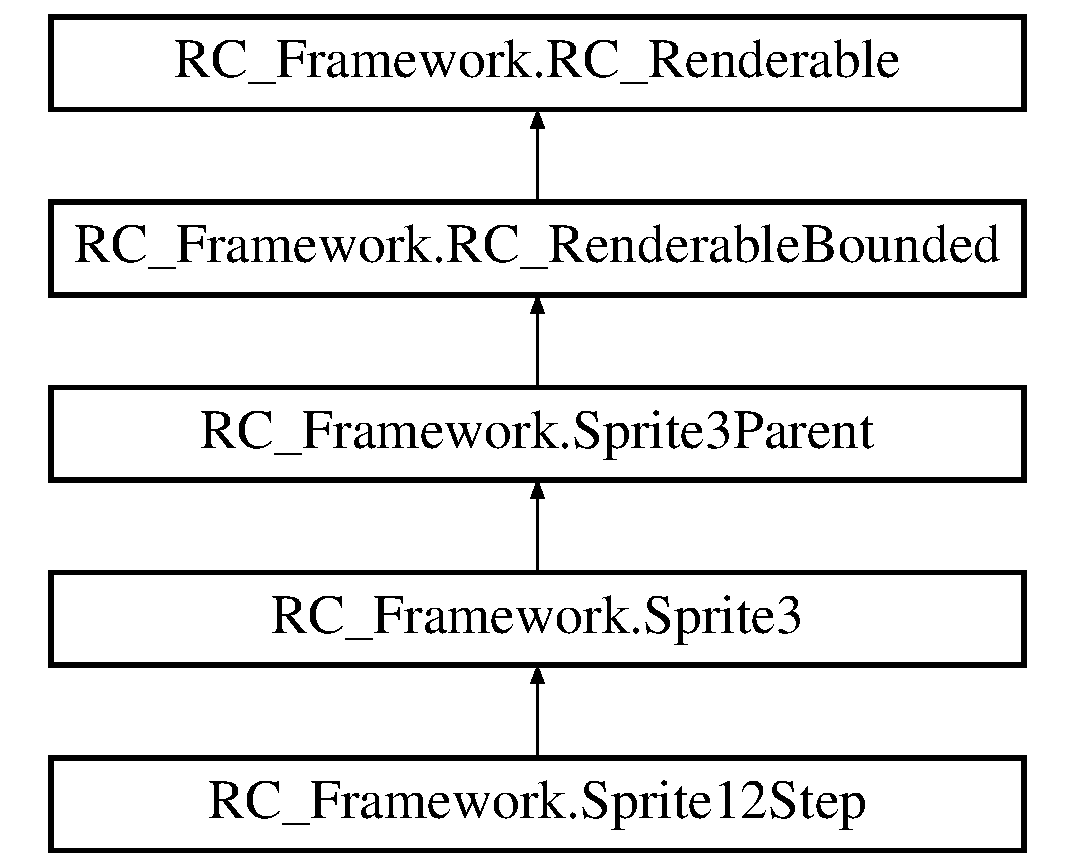
\includegraphics[height=5.000000cm]{class_r_c___framework_1_1_sprite3}
\end{center}
\end{figure}
\subsection*{Public Member Functions}
\begin{DoxyCompactItemize}
\item 
\mbox{\hyperlink{class_r_c___framework_1_1_sprite3_a92d70269202bf98ede05cbc45ca3690a}{Sprite3}} ()
\begin{DoxyCompactList}\small\item\em Default constructor \end{DoxyCompactList}\item 
\mbox{\hyperlink{class_r_c___framework_1_1_sprite3_a497f021ee596994c26f0d83135b676f5}{Sprite3}} (bool visibleZ, Texture2D texZ, float x, float y)
\begin{DoxyCompactList}\small\item\em Standard Constructor \end{DoxyCompactList}\item 
\mbox{\hyperlink{class_r_c___framework_1_1_sprite3_a5157f6fac4128e14e3a28ba540daec37}{Sprite3}} (bool visibleZ, Texture2D texZ, String nameZ, float x, float y)
\begin{DoxyCompactList}\small\item\em named Constructor with level \end{DoxyCompactList}\item 
override void \mbox{\hyperlink{class_r_c___framework_1_1_sprite3_a4ffc487d5c332dee276909dad3dba57a}{restore\+Position}} ()
\begin{DoxyCompactList}\small\item\em restore the current position \end{DoxyCompactList}\item 
override void \mbox{\hyperlink{class_r_c___framework_1_1_sprite3_ae4733340c18c8098b250418081020c6a}{save\+Position}} ()
\begin{DoxyCompactList}\small\item\em Save the current position \end{DoxyCompactList}\item 
string \mbox{\hyperlink{class_r_c___framework_1_1_sprite3_afa836f90205eb82c09f948e01c0e47ca}{get\+Name}} ()
\begin{DoxyCompactList}\small\item\em gets the sprite name if one was set or \char`\"{}\char`\"{} \end{DoxyCompactList}\item 
void \mbox{\hyperlink{class_r_c___framework_1_1_sprite3_a95f9492fffdbd603d9aa087b4bc108f4}{set\+Texture}} (Texture2D tw, bool compute\+New\+Size)
\begin{DoxyCompactList}\small\item\em set the texture -\/ and set a default texture width and height W\+A\+R\+N\+I\+NG if compute\+New\+Size is true all size information will be recomputed Xframes, Yframes W\+A\+R\+N\+I\+NG if compute\+New\+Size is false no size information will be recomputed Think about the value of compute\+New\+Size its not always that obvious \end{DoxyCompactList}\item 
Texture2D \mbox{\hyperlink{class_r_c___framework_1_1_sprite3_a32b080ce4ed442a34af48551b05c4847}{get\+Texture\+Base}} ()
\begin{DoxyCompactList}\small\item\em get the texturewrapper \end{DoxyCompactList}\item 
Texture2D \mbox{\hyperlink{class_r_c___framework_1_1_sprite3_a5a3eda5b5e64a44638051ece772411ca}{get\+Texture\+Frame}} ()
\item 
Rectangle \mbox{\hyperlink{class_r_c___framework_1_1_sprite3_a438ffa0b834a51a9f9cf35e372457d41}{image\+Rectangle}} ()
\begin{DoxyCompactList}\small\item\em Return a Rectangle structure which is the sprite boundary for screen graphic purposes I am not sure if this is used or of value any more (deprecated) \end{DoxyCompactList}\item 
Rectangle \mbox{\hyperlink{class_r_c___framework_1_1_sprite3_a1069512793423e1c5f3205d053e11d66}{get\+Bounding\+Box\+AA}} ()
\begin{DoxyCompactList}\small\item\em Return the axis aligned bounding box at the current position even if the display is rotated \end{DoxyCompactList}\item 
\mbox{\hyperlink{class_r_c___framework_1_1_polygon12}{Polygon12}} \mbox{\hyperlink{class_r_c___framework_1_1_sprite3_a9ed1e862b6f3f6a28f65b5c53fbb34e1}{set\+Bounding\+Poly\+From\+BB}} ()
\begin{DoxyCompactList}\small\item\em Gets a \mbox{\hyperlink{class_r_c___framework_1_1_polygon12}{Polygon12}} structure which is the non axis aligned bounding box from the \mbox{\hyperlink{class_r_c___framework_1_1_rect4}{Rect4}} its a fairly slow routine, if you use \mbox{\hyperlink{class_r_c___framework_1_1_sprite3_a1069512793423e1c5f3205d053e11d66}{get\+Bounding\+Box\+A\+A()}} anyway just do copy\+Rect4temp\+To\+B\+B() its faster \end{DoxyCompactList}\item 
void \mbox{\hyperlink{class_r_c___framework_1_1_sprite3_af5a02783f1305245a178fbe1cc1cc47a}{copy\+Rect4temp\+To\+Bounding\+Poly}} ()
\begin{DoxyCompactList}\small\item\em copies the temp rect4 structure to non axis aligned bounding box ~\newline
\end{DoxyCompactList}\item 
void \mbox{\hyperlink{class_r_c___framework_1_1_sprite3_ab430c66998577533366d5e4b1b85e2f4}{compute\+Bounding\+Poly\+From\+Pos}} ()
\begin{DoxyCompactList}\small\item\em Computes the bounding polygon from the offsets and position \end{DoxyCompactList}\item 
\mbox{\hyperlink{class_r_c___framework_1_1_polygon12}{Polygon12}} \mbox{\hyperlink{class_r_c___framework_1_1_sprite3_afd66805a5662cad934b912d4b204819d}{get\+Bounding\+Poly}} ()
\begin{DoxyCompactList}\small\item\em retreives the bounding pollygon -\/ which assumed that the user called necessary routines to set it one of\+: \end{DoxyCompactList}\item 
Vector2 \mbox{\hyperlink{class_r_c___framework_1_1_sprite3_a01208614a05673dd6b6d747910394657}{get\+Bounding\+Box\+Middle}} ()
\begin{DoxyCompactList}\small\item\em Return the mid point of the axis aligned bounding box at the current position \end{DoxyCompactList}\item 
bool \mbox{\hyperlink{class_r_c___framework_1_1_sprite3_a91ecfec14fcf4e3d45968c46f17fd83b}{collision}} (\mbox{\hyperlink{class_r_c___framework_1_1_sprite3}{Sprite3}} s2)
\begin{DoxyCompactList}\small\item\em Return true if two sprites axis aligned bounding boxes collide at their current locations \end{DoxyCompactList}\item 
Rectangle \mbox{\hyperlink{class_r_c___framework_1_1_sprite3_a50c663717778826a66395efd510aec62}{collision\+Rect}} (\mbox{\hyperlink{class_r_c___framework_1_1_sprite3}{Sprite3}} s2)
\begin{DoxyCompactList}\small\item\em Return a rectangle that represents a collision rectangle (the intersection of the two rectangles)\end{DoxyCompactList}\item 
Boolean \mbox{\hyperlink{class_r_c___framework_1_1_sprite3_addc1a2eb2b33095855d15652afac06e9}{inside}} (float x, float y)
\begin{DoxyCompactList}\small\item\em Return a boolean that is true if the point is inside the AA bounding box of the sprite\end{DoxyCompactList}\item 
Boolean \mbox{\hyperlink{class_r_c___framework_1_1_sprite3_abdaf66e3a0bcc82d446a2c3f059c3fba}{inside\+Or\+Eq}} (float x, float y)
\begin{DoxyCompactList}\small\item\em Return a boolean that is true if the point is inside or on the AA bounding box of the sprite\end{DoxyCompactList}\item 
override bool \mbox{\hyperlink{class_r_c___framework_1_1_sprite3_ab4c64556d7bcebf5ce538631ae9b5d6c}{scroll\+Move}} (float x, float y)
\begin{DoxyCompactList}\small\item\em Used to scroll the entire screen -\/ while preserving old position usually called in spritelist \end{DoxyCompactList}\item 
void \mbox{\hyperlink{class_r_c___framework_1_1_sprite3_a39a0fe699940c7d7f57971dd2edabe88}{move\+By\+Delta\+XY}} ()
\begin{DoxyCompactList}\small\item\em Moves the sprite by the delta x and delta y in delta\+Speed use \mbox{\hyperlink{class_r_c___framework_1_1_sprite3_a9a00bb05c798cc43c3518bb5ae6d0186}{set\+Delta\+Speed(\+Vector2 ds)}} to set the movement \end{DoxyCompactList}\item 
void \mbox{\hyperlink{class_r_c___framework_1_1_sprite3_a0cbdba681e9a06a6270415b1a527536e}{move\+By\+Delta\+XY}} (Vector2 ds)
\begin{DoxyCompactList}\small\item\em Moves the sprite by the delta x and delta y in delta\+Speed uses an input delta so no need to call \mbox{\hyperlink{class_r_c___framework_1_1_sprite3_a9a00bb05c798cc43c3518bb5ae6d0186}{set\+Delta\+Speed(\+Vector2 ds)}} \end{DoxyCompactList}\item 
void \mbox{\hyperlink{class_r_c___framework_1_1_sprite3_a6240d1baac5370a9be06ebaa4c188a95}{move\+By\+DeltaX}} (float dx)
\begin{DoxyCompactList}\small\item\em Moves the sprite by the delta x in dx used to separate x and y when using dx/dy movement mainly to assist in two part collision detection \end{DoxyCompactList}\item 
void \mbox{\hyperlink{class_r_c___framework_1_1_sprite3_a1f6400b76f55f9714cbbba19db329aa0}{move\+By\+DeltaY}} (float dy)
\begin{DoxyCompactList}\small\item\em Moves the sprite by the delta y in dy used to separate x and y when using dx/dy movement mainly to assist in two part collision detection \end{DoxyCompactList}\item 
bool \mbox{\hyperlink{class_r_c___framework_1_1_sprite3_abe2751690c88083e769e0742f6707fc8}{move\+To}} (Vector2 posZ, float speed, bool set\+Display\+Angle)
\begin{DoxyCompactList}\small\item\em Moves the sprite towards the position pos \end{DoxyCompactList}\item 
bool \mbox{\hyperlink{class_r_c___framework_1_1_sprite3_ad9e41fed1c73323a3375173c9be541be}{move\+To}} (\mbox{\hyperlink{class_r_c___framework_1_1_way_point}{Way\+Point}} way\+Point, bool set\+Display\+Angle)
\begin{DoxyCompactList}\small\item\em Moves the sprite towards the waypoint \end{DoxyCompactList}\item 
bool \mbox{\hyperlink{class_r_c___framework_1_1_sprite3_a7f4a44725a3873c534b0466b7b49a990}{move\+Way\+Point\+List}} (bool set\+Display\+Angle)
\begin{DoxyCompactList}\small\item\em Move the sprite around the waypoint list \end{DoxyCompactList}\item 
void \mbox{\hyperlink{class_r_c___framework_1_1_sprite3_a0dc780cf6c8438ad43880143e9e273c1}{move\+To\+Start\+Of\+Way\+Points}} ()
\begin{DoxyCompactList}\small\item\em Puts the sprite at the start of the waypoint list \end{DoxyCompactList}\item 
void \mbox{\hyperlink{class_r_c___framework_1_1_sprite3_a8566054426bf9eb7093c101a2c26407e}{move\+By\+Angle\+Speed}} ()
\begin{DoxyCompactList}\small\item\em Moves the sprite by the delta x and delta y in delta\+Speed \end{DoxyCompactList}\item 
void \mbox{\hyperlink{class_r_c___framework_1_1_sprite3_ad6501c04436015bde3919a8ca6d7d4a0}{adjust\+Angles}} ()
\begin{DoxyCompactList}\small\item\em Adjust \end{DoxyCompactList}\item 
void \mbox{\hyperlink{class_r_c___framework_1_1_sprite3_a07e6bec661635476eb17c60f72cfff68}{move\+By\+Angle\+Speed\+Limit}} (Rectangle r)
\begin{DoxyCompactList}\small\item\em Move with screen (or world wrap) \end{DoxyCompactList}\item 
Sprite\+Effects \mbox{\hyperlink{class_r_c___framework_1_1_sprite3_af559b399e3825aedda707573275f64df}{get\+Flip}} ()
\begin{DoxyCompactList}\small\item\em gets the flip parameter (which sets sprite effects for horizontal and vertical flipping) \end{DoxyCompactList}\item 
void \mbox{\hyperlink{class_r_c___framework_1_1_sprite3_a89a3746f82cb41211df31fc775654e8c}{set\+Flip}} (Sprite\+Effects se)
\begin{DoxyCompactList}\small\item\em sets the flip paramentser \end{DoxyCompactList}\item 
void \mbox{\hyperlink{class_r_c___framework_1_1_sprite3_ac7c6f7b2d84cfae1559eb4c84cb37f59}{set\+Width\+Height}} (float w, float h)
\begin{DoxyCompactList}\small\item\em sets the width and height of the sprite in display pixels \end{DoxyCompactList}\item 
void \mbox{\hyperlink{class_r_c___framework_1_1_sprite3_a05dbc29987c0c2552cb69e81ea3fcdab}{set\+Width\+Height\+To\+Tex}} ()
\begin{DoxyCompactList}\small\item\em sets the width and height of the sprite to what was read in from the texture This is usefull when you want the whole image \end{DoxyCompactList}\item 
void \mbox{\hyperlink{class_r_c___framework_1_1_sprite3_a6c0cc3a2227564aba7ee4d66d0c620fe}{set\+Width}} (float w)
\begin{DoxyCompactList}\small\item\em Just set the sprite width in display pixels \end{DoxyCompactList}\item 
void \mbox{\hyperlink{class_r_c___framework_1_1_sprite3_ad1f24cf43143791cb73c80a4af1881f0}{set\+Height}} (float h)
\begin{DoxyCompactList}\small\item\em just set the sprite height in display pixels \end{DoxyCompactList}\item 
float \mbox{\hyperlink{class_r_c___framework_1_1_sprite3_a0368a20bd12250f8f55c0788531e454a}{get\+Width}} ()
\begin{DoxyCompactList}\small\item\em get the width in display pixels \end{DoxyCompactList}\item 
float \mbox{\hyperlink{class_r_c___framework_1_1_sprite3_a67a30fb7ba96da33d63134b34e6dbc0c}{get\+Height}} ()
\begin{DoxyCompactList}\small\item\em get the height in display pixels \end{DoxyCompactList}\item 
void \mbox{\hyperlink{class_r_c___framework_1_1_sprite3_aced9c5f15e8334fd68852b3c9e67f2d8}{set\+Width\+Height\+Of\+Tex}} (float w, float h)
\begin{DoxyCompactList}\small\item\em This sets the usefull part of the texture (which is assumed to be the top left bit) its necessary because not all textures conform to the power of 2 rule and are upsized to a power of two \end{DoxyCompactList}\item 
void \mbox{\hyperlink{class_r_c___framework_1_1_sprite3_ad1f6bebc12d9d8f9bdf4ba13f3907bc3}{set\+Width\+Height\+Of\+Tex\+To\+Tex}} ()
\begin{DoxyCompactList}\small\item\em Just sets the active part of the texture to the whole texture \end{DoxyCompactList}\item 
virtual void \mbox{\hyperlink{class_r_c___framework_1_1_sprite3_ac73292a1b053056aa28ecae03165c71d}{set\+Image\+Source}} (Rectangle r)
\begin{DoxyCompactList}\small\item\em Sets a source image for the sprite (usually less than the total texture) W\+A\+R\+N\+I\+NG This will alter the Xframes, Yframes \end{DoxyCompactList}\item 
Rectangle \mbox{\hyperlink{class_r_c___framework_1_1_sprite3_a87dbfe3899e44fc7376837fe4cff0bd6}{get\+Image\+Source}} ()
\begin{DoxyCompactList}\small\item\em returns the image source parameter for the sprite for the current frame use \mbox{\hyperlink{class_r_c___framework_1_1_sprite3_a376a1cca122797eb306bc81d31e91551}{get\+Actual\+Image\+Source()}} \end{DoxyCompactList}\item 
Rectangle \mbox{\hyperlink{class_r_c___framework_1_1_sprite3_a376a1cca122797eb306bc81d31e91551}{get\+Actual\+Image\+Source}} ()
\begin{DoxyCompactList}\small\item\em Where we get the sprite image from not intended for external use \end{DoxyCompactList}\item 
override void \mbox{\hyperlink{class_r_c___framework_1_1_sprite3_a79b8e18ee29cd62719307a059e4cb6df}{Draw}} (Sprite\+Batch sb)
\begin{DoxyCompactList}\small\item\em Draws the sprite if it is Visible (ie if the visible property is set) \end{DoxyCompactList}\item 
void \mbox{\hyperlink{class_r_c___framework_1_1_sprite3_afc737761beac47c71402bea9f5cc0b2a}{prepare\+To\+Draw}} ()
\begin{DoxyCompactList}\small\item\em Prepares the internal variables src,dest and rotate\+Image for drawing It can be used for -\/ writing virtual screen handlers that zoom, resize and pan \end{DoxyCompactList}\item 
void \mbox{\hyperlink{class_r_c___framework_1_1_sprite3_a4a9fc342f033b500edb18fbf9b921879}{draw}} (Sprite\+Batch sb)
\begin{DoxyCompactList}\small\item\em Draws the sprite if it is Visible (ie if the visible property is set) \end{DoxyCompactList}\item 
Vector2 \mbox{\hyperlink{class_r_c___framework_1_1_sprite3_aae022ecd2e51d1ad3654854b8594494f}{get\+Rotate\+Image}} ()
\begin{DoxyCompactList}\small\item\em Gets the point about which to rotate the image in Image co-\/ordinates \end{DoxyCompactList}\item 
void \mbox{\hyperlink{class_r_c___framework_1_1_sprite3_a0901ebb278e50e5244e4b7f0fbd57242}{set\+BB}} (float bb\+Xoffset, float bb\+Yoffset, float bb\+WidthZ, float bb\+HeightZ)
\begin{DoxyCompactList}\small\item\em Sets the bounding box relative to the hotspot (or position) if the hotspot is in the middle of the source image there is a fair chance that bb.\+X and bb.\+Y will be negative \end{DoxyCompactList}\item 
void \mbox{\hyperlink{class_r_c___framework_1_1_sprite3_a352f91941f5ca2df898d966564e4c875}{set\+B\+B\+To\+Texture}} ()
\begin{DoxyCompactList}\small\item\em lol for basic sprites set the BB to the texture with and height \end{DoxyCompactList}\item 
void \mbox{\hyperlink{class_r_c___framework_1_1_sprite3_aca02729a3919f4f31c4c63f814ea0150}{set\+B\+B\+To\+WH}} ()
\begin{DoxyCompactList}\small\item\em set the bounding box to the width and height of the sprite typically this is a bounding box that follows the image boundary with a hotspot in the image top left corner \end{DoxyCompactList}\item 
void \mbox{\hyperlink{class_r_c___framework_1_1_sprite3_a820e5316676eee1ef5fccdc9ac07cf15}{set\+B\+B\+To\+Frame\+In\+Tex}} ()
\begin{DoxyCompactList}\small\item\em set the bounding box to the width and height of A single frame typically this is a bounding box that follows the image boundary with a hotspot in the image top left corner \end{DoxyCompactList}\item 
void \mbox{\hyperlink{class_r_c___framework_1_1_sprite3_ad599fbce8c9402618ead1232fc9d0539}{set\+B\+B\+Fraction\+Of\+Tex\+Centered}} (float f)
\begin{DoxyCompactList}\small\item\em Sets the bounding box to a fraction of the texture width and height eg set\+B\+B\+To\+Fraction(0.\+6) would creat a small bounding box whose dimensions are 0.\+6 of the full sprite dimensions with the bboffset sane if the hotspot is 0,0 \end{DoxyCompactList}\item 
void \mbox{\hyperlink{class_r_c___framework_1_1_sprite3_a899837f4fa3d7c5736a31b30de845707}{set\+B\+B\+Fraction\+Of\+Tex}} (float f, int xoffset, int yoffset)
\begin{DoxyCompactList}\small\item\em Sets the bounding box to a fraction of the texture width and height eg set\+B\+B\+To\+Fraction(0.\+6, 5, 7) would creat a small bounding box whose dimensions are 0.\+6 of the full sprite dimensions with the bboffset at 5,7 \end{DoxyCompactList}\item 
void \mbox{\hyperlink{class_r_c___framework_1_1_sprite3_a4c84dca0a120793e378451cefefb4183}{set\+B\+Band\+H\+S\+Fraction\+Of\+Tex\+Centered}} (float f)
\begin{DoxyCompactList}\small\item\em Sets the bounding box to a fraction of the texture width and height eg set\+B\+B\+To\+Fraction(0.\+6) would creat a small bounding box whose dimensions are 0.\+6 of the full sprite dimensions with the bboffset sane if the hotspot is 0,0 \end{DoxyCompactList}\item 
Rectangle \mbox{\hyperlink{class_r_c___framework_1_1_sprite3_a16549a56813ed7daed2a64f6d2c3fdaf}{get\+BB}} ()
\begin{DoxyCompactList}\small\item\em Get the bouding rectange in screen co ordinates -\/ relative to the sprite pos \end{DoxyCompactList}\item 
void \mbox{\hyperlink{class_r_c___framework_1_1_sprite3_a2551e6efc55ccfb3596b0f5bff398fc1}{set\+H\+Soffset}} (Vector2 offset)
\begin{DoxyCompactList}\small\item\em Set the hotspot offset Note that this is in original image pixels not pixels after resize \end{DoxyCompactList}\item 
Vector2 \mbox{\hyperlink{class_r_c___framework_1_1_sprite3_a8f296827e1659e0b370699146d18536b}{get\+H\+S\+Offset}} ()
\begin{DoxyCompactList}\small\item\em set the Hotspot offset \end{DoxyCompactList}\item 
virtual void \mbox{\hyperlink{class_r_c___framework_1_1_sprite3_a0b6d0934cd9eea34b1d517a1d09102be}{draw\+BB}} (Sprite\+Batch sb, Color c)
\begin{DoxyCompactList}\small\item\em draws a bounding box \end{DoxyCompactList}\item 
void \mbox{\hyperlink{class_r_c___framework_1_1_sprite3_aa82450ed1a30116c7419e79c34c374f4}{draw\+HS}} (Sprite\+Batch sb, Color c)
\begin{DoxyCompactList}\small\item\em Draws the hotspot/position of the sprite \end{DoxyCompactList}\item 
void \mbox{\hyperlink{class_r_c___framework_1_1_sprite3_a1f1acda2345b760c30d0f1c4c0815d4c}{draw\+Info}} (Sprite\+Batch sb, Color color\+BB, Color color\+HS)
\begin{DoxyCompactList}\small\item\em draw bounding box and hotspot \end{DoxyCompactList}\item 
void \mbox{\hyperlink{class_r_c___framework_1_1_sprite3_a33bc86bddbc57f002991ccf17c97d80a}{draw\+Bounding\+Sphere}} (Sprite\+Batch sb, Color color\+BS)
\begin{DoxyCompactList}\small\item\em draw bounding sphere if not zero \end{DoxyCompactList}\item 
void \mbox{\hyperlink{class_r_c___framework_1_1_sprite3_a3787b8d78c1aedee770e6d2871e78156}{draw\+Bounding\+Poly}} (Sprite\+Batch sb, Color color\+BB, Color color\+HS)
\begin{DoxyCompactList}\small\item\em Draws the bounding polygon and the hotspot if it exists \end{DoxyCompactList}\item 
void \mbox{\hyperlink{class_r_c___framework_1_1_sprite3_a0ef49f4248eee1b81e48a2a8125fa477}{draw\+Rect4}} (Sprite\+Batch sb, Color c)
\begin{DoxyCompactList}\small\item\em For debugging only to make sure rotations are where they are expected to be You must have called get bounding box Axis aligned first \end{DoxyCompactList}\item 
void \mbox{\hyperlink{class_r_c___framework_1_1_sprite3_a9a00bb05c798cc43c3518bb5ae6d0186}{set\+Delta\+Speed}} (Vector2 ds)
\begin{DoxyCompactList}\small\item\em Set a speed vector for the deltax/deltay move system \end{DoxyCompactList}\item 
Vector2 \mbox{\hyperlink{class_r_c___framework_1_1_sprite3_a07bcebd23820bced67a5d2a34eeda633}{get\+Delta\+Speed}} ()
\begin{DoxyCompactList}\small\item\em get the speed deltas for the deltax deltay move system \end{DoxyCompactList}\item 
float \mbox{\hyperlink{class_r_c___framework_1_1_sprite3_a71a24dd1eb93a65918e2b1db390a5546}{get\+Move\+Angle\+Radians}} ()
\begin{DoxyCompactList}\small\item\em Get the current movemnet angle for the angle / speed move system \end{DoxyCompactList}\item 
void \mbox{\hyperlink{class_r_c___framework_1_1_sprite3_a323f04ef41bc129dee67fa3b4a5cab42}{set\+Move\+Angle\+Radians}} (float m)
\begin{DoxyCompactList}\small\item\em Set the current movemnet angle in radians for the angle / speed move system \end{DoxyCompactList}\item 
void \mbox{\hyperlink{class_r_c___framework_1_1_sprite3_a6704e7b0ad3c2b828975cfe1c9cf73a3}{set\+Move\+Angle\+Degrees}} (float m)
\begin{DoxyCompactList}\small\item\em Set the current movemnet angle for the angle / speed move system \end{DoxyCompactList}\item 
float \mbox{\hyperlink{class_r_c___framework_1_1_sprite3_a1534ae3b4f4a7b075661e0d644d589cf}{get\+Move\+Speed}} ()
\begin{DoxyCompactList}\small\item\em Get the current movemnet speed for the angle / speed move system \end{DoxyCompactList}\item 
void \mbox{\hyperlink{class_r_c___framework_1_1_sprite3_a630b8d8f2eda0fc820bf76a2c65f0671}{set\+Move\+Speed}} (float m)
\begin{DoxyCompactList}\small\item\em Set the current movemnet speed for the angle / speed move system \end{DoxyCompactList}\item 
float \mbox{\hyperlink{class_r_c___framework_1_1_sprite3_a7f311c885100d7a2164549158d90d927}{get\+Display\+Angle\+Radians}} ()
\begin{DoxyCompactList}\small\item\em get display angle in radians \end{DoxyCompactList}\item 
void \mbox{\hyperlink{class_r_c___framework_1_1_sprite3_a3e00764164dccc3eb6104e5ec643033a}{set\+Display\+Angle\+Radians}} (float d)
\begin{DoxyCompactList}\small\item\em set display angle in radians \end{DoxyCompactList}\item 
void \mbox{\hyperlink{class_r_c___framework_1_1_sprite3_a13036025a68f4353c2b9014d8634e836}{set\+Display\+Angle\+Degrees}} (float d)
\begin{DoxyCompactList}\small\item\em Set display angle in degrees \end{DoxyCompactList}\item 
void \mbox{\hyperlink{class_r_c___framework_1_1_sprite3_a2ec8cfce2feb2f1e648131e03099b147}{set\+Display\+Angle\+Offset}} (float d)
\begin{DoxyCompactList}\small\item\em set the display angle offset in radians -\/ which is the angle added to the display\+Angle to make the sprite face in direction 0 \end{DoxyCompactList}\item 
void \mbox{\hyperlink{class_r_c___framework_1_1_sprite3_a6269a6c50ca875525156d347b216e491}{set\+Display\+Angle\+Offset\+Degrees}} (float d)
\begin{DoxyCompactList}\small\item\em set the display angle offset -\/ which is the angle added to the display\+Angle to make the sprite face in direction 0 \end{DoxyCompactList}\item 
float \mbox{\hyperlink{class_r_c___framework_1_1_sprite3_aad5d5ae96adc595d808baf24a283982e}{get\+Display\+Angle\+Offset}} ()
\begin{DoxyCompactList}\small\item\em get the display angle offset \end{DoxyCompactList}\item 
void \mbox{\hyperlink{class_r_c___framework_1_1_sprite3_aab8c41c05cad46205425cfdb86b60e56}{set\+Xframes}} (int f)
\begin{DoxyCompactList}\small\item\em Set the number of horizontal frames of animation \end{DoxyCompactList}\item 
void \mbox{\hyperlink{class_r_c___framework_1_1_sprite3_a248e1776ffd7be872288f73fb7caeadd}{set\+Yframes}} (int f)
\begin{DoxyCompactList}\small\item\em Set the number of vertical frames of animation \end{DoxyCompactList}\item 
int \mbox{\hyperlink{class_r_c___framework_1_1_sprite3_ac03a161791879ccf0758985c9dc49cce}{get\+Yframes}} ()
\begin{DoxyCompactList}\small\item\em get the number of vertical frames of animation \end{DoxyCompactList}\item 
int \mbox{\hyperlink{class_r_c___framework_1_1_sprite3_a838ca2253128f4f1099fa1ae24fe1fdf}{get\+Xframes}} ()
\begin{DoxyCompactList}\small\item\em set the number of vertical frames of animation \end{DoxyCompactList}\item 
int \mbox{\hyperlink{class_r_c___framework_1_1_sprite3_afce769592e5683b522e77fa1edf9e81e}{get\+Xframe}} ()
\begin{DoxyCompactList}\small\item\em get the current horizontal frame \end{DoxyCompactList}\item 
int \mbox{\hyperlink{class_r_c___framework_1_1_sprite3_a909a64848da044a82bc9e3467ea28ace}{get\+Yframe}} ()
\begin{DoxyCompactList}\small\item\em get the current vertical frame \end{DoxyCompactList}\item 
int \mbox{\hyperlink{class_r_c___framework_1_1_sprite3_a4c0a6cf29709e9c6f8ead39eea215f4b}{get\+Frame}} ()
\begin{DoxyCompactList}\small\item\em Get the current frame number which is an index into the animation frame sequence data updated by set\+Animation\+Sequence \end{DoxyCompactList}\item 
void \mbox{\hyperlink{class_r_c___framework_1_1_sprite3_a946e99f3317d07ce6a098c4b435e1689}{set\+Yframe}} (int f)
\begin{DoxyCompactList}\small\item\em set the current vertical frame \end{DoxyCompactList}\item 
void \mbox{\hyperlink{class_r_c___framework_1_1_sprite3_a56a7afacc321c80d0dfb1d9c5933f7df}{set\+Xframe}} (int f)
\begin{DoxyCompactList}\small\item\em Set the current horizontal frame \end{DoxyCompactList}\item 
void \mbox{\hyperlink{class_r_c___framework_1_1_sprite3_a552be0daafb94d0cc7802a10539e5032}{set\+Frame}} (int f)
\begin{DoxyCompactList}\small\item\em Set the current frame number which is an index into the animation frame sequence data updated by set\+Animation\+Sequence \end{DoxyCompactList}\item 
void \mbox{\hyperlink{class_r_c___framework_1_1_sprite3_a2688823142342a7d1b2aaf91b8f5cc66}{set\+Animation\+Sequence}} (Vector2\mbox{[}$\,$\mbox{]} anim\+Seq, int first\+FrameZ, int last\+FrameZ, int ticks\+Between\+FramesZ)
\begin{DoxyCompactList}\small\item\em Set an animation sequenece \end{DoxyCompactList}\item 
void \mbox{\hyperlink{class_r_c___framework_1_1_sprite3_aaba067bf7bc24cd0acd437a057a69eec}{animation\+Tick}} (Game\+Time game\+Time)
\begin{DoxyCompactList}\small\item\em Upadate the animation sequence This routine is usually run in the update routine this routine now has game\+Time as a parameter \end{DoxyCompactList}\item 
void \mbox{\hyperlink{class_r_c___framework_1_1_sprite3_a280b1377c4b22b183c82956efa33c9e5}{set\+Anim\+Finished}} (int what\+To\+Do)
\begin{DoxyCompactList}\small\item\em What to do when the animation is finished 0=loop 1=set sprite invisible 2=set sprite inactive and invisible \end{DoxyCompactList}\item 
void \mbox{\hyperlink{class_r_c___framework_1_1_sprite3_ab181bdcfd7b9fcb12a931c13d2649d93}{animation\+Start}} ()
\begin{DoxyCompactList}\small\item\em Set the start parameters for the animation sequence \end{DoxyCompactList}\item 
void \mbox{\hyperlink{class_r_c___framework_1_1_sprite3_abaab134b0035e614af80fa1755118fd2}{animation\+Start}} (int ticksZ, int frameZ)
\begin{DoxyCompactList}\small\item\em Set the start parameters for the animation sequence allowing for some additional information \end{DoxyCompactList}\item 
void \mbox{\hyperlink{class_r_c___framework_1_1_sprite3_a03369c23f152dc9720174e5053acd33f}{set\+Fade\+Details}} (bool fadeQ, Color fade\+From\+ColourQ, Color fade\+To\+ColourQ, int fade\+TicksQ, bool make\+InactiveQ)
\item 
void \mbox{\hyperlink{class_r_c___framework_1_1_sprite3_a2710ebb2e7b64a1ce4ce91aaf81f5fce}{do\+The\+Fade}} ()
\item 
float \mbox{\hyperlink{class_r_c___framework_1_1_sprite3_a58e467760eaf53fa02f50fb4129861c3}{distance\+To}} (\mbox{\hyperlink{class_r_c___framework_1_1_sprite3}{Sprite3}} sprite)
\begin{DoxyCompactList}\small\item\em Distance to another sprite \end{DoxyCompactList}\item 
float \mbox{\hyperlink{class_r_c___framework_1_1_sprite3_ab41ca8d75520f2b6e11ba943d7eb3f77}{distance\+To}} (Vector2 point)
\begin{DoxyCompactList}\small\item\em Distance to an arbitary point \end{DoxyCompactList}\item 
void \mbox{\hyperlink{class_r_c___framework_1_1_sprite3_a92e3abec80772414657159820d45491a}{align\+Display\+Angle}} ()
\begin{DoxyCompactList}\small\item\em Aligns the display angle to the sprites current movement angle based on oldpos -\/ only works if the sprite is actually moving in a way that old\+Pos is updated correctly so use set\+Pos to set position (only one per update call) \end{DoxyCompactList}\item 
float \mbox{\hyperlink{class_r_c___framework_1_1_sprite3_a5354cb9f7ec64fa47814f67ee05d5fa5}{angle\+To}} (\mbox{\hyperlink{class_r_c___framework_1_1_sprite3}{Sprite3}} s)
\begin{DoxyCompactList}\small\item\em computes the angle to another sprite \end{DoxyCompactList}\item 
float \mbox{\hyperlink{class_r_c___framework_1_1_sprite3_a61485db626575e2a63c7ba078f84d46d}{angle\+To}} (Vector2 point)
\begin{DoxyCompactList}\small\item\em computes the angle to an arbitary point \end{DoxyCompactList}\item 
bool \mbox{\hyperlink{class_r_c___framework_1_1_sprite3_af3c0f0e95f498147b74322f3ef919005}{get\+Active}} ()
\begin{DoxyCompactList}\small\item\em get the active flag \end{DoxyCompactList}\item 
void \mbox{\hyperlink{class_r_c___framework_1_1_sprite3_a6e007701b261f3c293389e5094513faf}{set\+Active}} (bool activeZ)
\begin{DoxyCompactList}\small\item\em set the active flag \end{DoxyCompactList}\item 
void \mbox{\hyperlink{class_r_c___framework_1_1_sprite3_a9299af8d2e5277dd0e810389a7ed831c}{set\+Active\+And\+Visible}} (bool activeZ)
\begin{DoxyCompactList}\small\item\em set the active flag \end{DoxyCompactList}\item 
void \mbox{\hyperlink{class_r_c___framework_1_1_sprite3_ab849638ba60bac0f9accbd4091f95d1e}{set\+Ticks\+To\+Visible}} (int \mbox{\hyperlink{class_r_c___framework_1_1_sprite3_a59474528cccad4b750e2b72a5f8cf585}{ticks}})
\begin{DoxyCompactList}\small\item\em sets the number if ticks till the sprite becomes visible \end{DoxyCompactList}\item 
void \mbox{\hyperlink{class_r_c___framework_1_1_sprite3_abb634dc79e4094b58b566ef7d8aca35b}{set\+Ticks\+To\+Invisible}} (int \mbox{\hyperlink{class_r_c___framework_1_1_sprite3_a59474528cccad4b750e2b72a5f8cf585}{ticks}}, bool inactive)
\begin{DoxyCompactList}\small\item\em Sets the ticks untill the sprite becomes invisible optionally inactive as well to use it you must call \mbox{\hyperlink{class_r_c___framework_1_1_sprite3_aa6a483f4fdcd1ed260bd72f60a07834d}{tick()}} in update for the sprite \end{DoxyCompactList}\item 
virtual void \mbox{\hyperlink{class_r_c___framework_1_1_sprite3_aa6a483f4fdcd1ed260bd72f60a07834d}{tick}} ()
\begin{DoxyCompactList}\small\item\em Tick the visible / invisible ticker Tick is used in sprite 3 to make a sprite visible after a certain time see the routine set\+Ticks\+To\+Visible to set the tick counter \end{DoxyCompactList}\item 
override void \mbox{\hyperlink{class_r_c___framework_1_1_sprite3_a5473d37c4f1f44fa1685dd64c82dfd8c}{Update}} (Game\+Time game\+Time)
\end{DoxyCompactItemize}
\subsection*{Public Attributes}
\begin{DoxyCompactItemize}
\item 
const string \mbox{\hyperlink{class_r_c___framework_1_1_sprite3_af4a00055db200e357c65f9b289989ba5}{Sprite\+Version}} =\char`\"{}V3.\+18.\+1\char`\"{}
\begin{DoxyCompactList}\small\item\em Just a version to help code controll \end{DoxyCompactList}\item 
int \mbox{\hyperlink{class_r_c___framework_1_1_sprite3_a569b5506e5da155612f938e414d40c0b}{kind}}
\begin{DoxyCompactList}\small\item\em this variable called kind is available for use by user code \end{DoxyCompactList}\item 
int \mbox{\hyperlink{class_r_c___framework_1_1_sprite3_a390f0fa7f5de0cb734e313b31551b9c3}{state}}
\begin{DoxyCompactList}\small\item\em this variable called state is available for use by user code \end{DoxyCompactList}\item 
string \mbox{\hyperlink{class_r_c___framework_1_1_sprite3_a0b0ba2dfebf13a8ecf6ef372e3048f3c}{name}}
\begin{DoxyCompactList}\small\item\em Used by user for id or text purposes \end{DoxyCompactList}\item 
float \mbox{\hyperlink{class_r_c___framework_1_1_sprite3_a4428b9c3efc3f675f04df8141dc6e108}{score}}
\begin{DoxyCompactList}\small\item\em this variable called score is available for use by user code \end{DoxyCompactList}\item 
int \mbox{\hyperlink{class_r_c___framework_1_1_sprite3_af2d07d57951fed3fd45129d58590974a}{var\+Int0}}
\begin{DoxyCompactList}\small\item\em variables called var\+Int0, var\+Int1, var\+Int2 are available for use by user code there is also tagint and tag from renderable -\/ they are sort of duplicates \end{DoxyCompactList}\item 
int \mbox{\hyperlink{class_r_c___framework_1_1_sprite3_a76f69d382ff8046c88681fe212a99176}{var\+Int1}}
\begin{DoxyCompactList}\small\item\em available for use by user code \end{DoxyCompactList}\item 
int \mbox{\hyperlink{class_r_c___framework_1_1_sprite3_a6dda4cde780442d3d2f226158fee5a11}{var\+Int2}}
\begin{DoxyCompactList}\small\item\em available for use by user code \end{DoxyCompactList}\item 
int \mbox{\hyperlink{class_r_c___framework_1_1_sprite3_ae6cca5521f73ec073caa66b816ab8408}{var\+Int3}}
\begin{DoxyCompactList}\small\item\em available for use by user code \end{DoxyCompactList}\item 
int \mbox{\hyperlink{class_r_c___framework_1_1_sprite3_a461eb5bc92dd3eff6daff40147f060eb}{var\+Int4}}
\begin{DoxyCompactList}\small\item\em available for use by user code \end{DoxyCompactList}\item 
bool \mbox{\hyperlink{class_r_c___framework_1_1_sprite3_a77c5b7c794daacbd31c49f83e40978f9}{var\+Bool0}}
\begin{DoxyCompactList}\small\item\em these variables called var\+Bool0, var\+Bool1 are available for use by user code \end{DoxyCompactList}\item 
bool \mbox{\hyperlink{class_r_c___framework_1_1_sprite3_a5f9e5ed1f2c6b498eb2ca9e461c8bebc}{var\+Bool1}}
\begin{DoxyCompactList}\small\item\em available for use by user code \end{DoxyCompactList}\item 
float \mbox{\hyperlink{class_r_c___framework_1_1_sprite3_aa90e0f3319e1d183780eaa4570d6bf2b}{var\+Float1}}
\begin{DoxyCompactList}\small\item\em available for use by user code single floatig point number \end{DoxyCompactList}\item 
Vector2 \mbox{\hyperlink{class_r_c___framework_1_1_sprite3_a7a99bed1590ff1e7e1f7c52a4a53c37e}{target}}
\begin{DoxyCompactList}\small\item\em this variable called target is available for use by user code \end{DoxyCompactList}\item 
int \mbox{\hyperlink{class_r_c___framework_1_1_sprite3_abe8d4ab8316448c8d9ff2da22b680380}{hit\+Points}}
\begin{DoxyCompactList}\small\item\em this variable called hit\+Points is available for use by user code it is also used by the attached renderable \mbox{\hyperlink{class_r_c___framework_1_1_health_bar}{Health\+Bar}} if one is active \end{DoxyCompactList}\item 
int \mbox{\hyperlink{class_r_c___framework_1_1_sprite3_a7177e23ee5d4dd93ca4972e9798be680}{max\+Hit\+Points}}
\begin{DoxyCompactList}\small\item\em this variable called max\+Hit\+Points is available for use by user code it may get used by an attached renderable to draw a health bar (or any other purpose) it is used by the attached renderable \mbox{\hyperlink{class_r_c___framework_1_1_health_bar}{Health\+Bar}} \end{DoxyCompactList}\item 
float \mbox{\hyperlink{class_r_c___framework_1_1_sprite3_a6f76b1e09c665b5a930cb86c34c86429}{bounding\+Sphere\+Radius}}
\begin{DoxyCompactList}\small\item\em bounding Sphere Radius for user to use this is in screen pixels not source pixels any resizing must be done by the user \end{DoxyCompactList}\item 
Sprite\+Effects \mbox{\hyperlink{class_r_c___framework_1_1_sprite3_a2320b0a1f529f8b9998377a5690c2878}{flip}} = Sprite\+Effects.\+None
\begin{DoxyCompactList}\small\item\em the direction of the sprite Sprite\+Effects.\+None, Sprite\+Effects.\+Flip\+Horizontaly, Sprite\+Effects.\+Flip\+Vertically \end{DoxyCompactList}\item 
float \mbox{\hyperlink{class_r_c___framework_1_1_sprite3_aed8fd08f1d911727fb48d3c456be713a}{display\+Angle}}
\begin{DoxyCompactList}\small\item\em the display angle in radians -\/ which may or may not be the move angle should be set using set\+Display\+Angle(float d) \end{DoxyCompactList}\item 
float \mbox{\hyperlink{class_r_c___framework_1_1_sprite3_aafcde3bd32143744faf410c304a07f2d}{display\+Angle\+Offset}}
\begin{DoxyCompactList}\small\item\em the display angle offset in radians Added to display angle to make the sprite \char`\"{}point in direction 0\char`\"{} should be set using \mbox{\hyperlink{class_r_c___framework_1_1_sprite3_a2ec8cfce2feb2f1e648131e03099b147}{set\+Display\+Angle\+Offset(float d)}} \end{DoxyCompactList}\item 
\mbox{\hyperlink{class_r_c___framework_1_1_frame_source}{Frame\+Source}} \mbox{\hyperlink{class_r_c___framework_1_1_sprite3_a052b6b4879f526456238accb371373a0}{frame\+Source}} = null
\begin{DoxyCompactList}\small\item\em Animation system can have various values the possible behaviours are\+: \end{DoxyCompactList}\item 
\mbox{\hyperlink{class_r_c___framework_1_1_rect4}{Rect4}} \mbox{\hyperlink{class_r_c___framework_1_1_sprite3_a4fedf0e3c61d7960064f3588a9cc8a93}{bb\+Temp}}
\begin{DoxyCompactList}\small\item\em Internal structure so one can check bounding box positions this turns out to be a usefull variable for debugging and display also it can be moved to bounding\+Poly for a non AA bounding box using Util2.\+Polygon12(\+Rect4 r) constructor \end{DoxyCompactList}\item 
\mbox{\hyperlink{class_r_c___framework_1_1_polygon12}{Polygon12}} \mbox{\hyperlink{class_r_c___framework_1_1_sprite3_a38eaba03c71e388c288d36fbdf9cf9b6}{bounding\+Poly\+Offsets}} =null
\begin{DoxyCompactList}\small\item\em Advanced Bounding box polygon offsets -\/ its in screen pixels Needs the polygon collision utility to use only partly supported \end{DoxyCompactList}\item 
\mbox{\hyperlink{class_r_c___framework_1_1_polygon12}{Polygon12}} \mbox{\hyperlink{class_r_c___framework_1_1_sprite3_a539da11d835c64da3a78039cd05942e9}{bounding\+Poly}} =null
\begin{DoxyCompactList}\small\item\em Advanced Bounding box not axis aligned -\/ its in screen pixels Needs the polygon collision utility to use only partly supported updated by routine compute\+Bounding\+Poly\+From\+Pos \end{DoxyCompactList}\item 
Rectangle \mbox{\hyperlink{class_r_c___framework_1_1_sprite3_aec76c65582a5d71056a0d5f44f2e2906}{src}}
\begin{DoxyCompactList}\small\item\em Internal source rectangle -\/ do not touch unless you know what you are doing source of image \end{DoxyCompactList}\item 
Rectangle \mbox{\hyperlink{class_r_c___framework_1_1_sprite3_ab2d852bf859c3d55bcf6517797b69dc6}{dest}}
\begin{DoxyCompactList}\small\item\em Internal destination rectangle -\/ do not touch unless you know what you are doing destination of image \end{DoxyCompactList}\end{DoxyCompactItemize}
\subsection*{Protected Attributes}
\begin{DoxyCompactItemize}
\item 
Texture2D \mbox{\hyperlink{class_r_c___framework_1_1_sprite3_ac69869c54b541f68ac23464874a4e91f}{tex\+Base}}
\begin{DoxyCompactList}\small\item\em The sprites texture2d for basic sprites -\/ do not change it arbitarily use set\+Texture(\+Texture2\+D tw) routine instead to preserve frame information \end{DoxyCompactList}\item 
Texture2D \mbox{\hyperlink{class_r_c___framework_1_1_sprite3_a5b3ed08cfae3aba31834ad0c16c98ed3}{tex\+Frame}}
\begin{DoxyCompactList}\small\item\em The sprites texture2d for sprites using a \mbox{\hyperlink{class_r_c___framework_1_1_frame_source}{Frame\+Source}} usually in all other cases it is identical to tex\+Base do not change it arbitarily use set\+Texture(\+Texture2\+D tw) routine instead to preserve frame information it is updated frame by frame when frame\+Source is used \end{DoxyCompactList}\item 
Vector2 \mbox{\hyperlink{class_r_c___framework_1_1_sprite3_a085b269f8bcef70e2e90cc6473d6d9f0}{delta\+Speed}}
\begin{DoxyCompactList}\small\item\em movement vector when using the deltax deltay movement system \end{DoxyCompactList}\item 
float \mbox{\hyperlink{class_r_c___framework_1_1_sprite3_a21a2dd7d771adeacb93f54e16c70809a}{move\+Angle}}
\begin{DoxyCompactList}\small\item\em the movement angle in radians if using the angle / speed movement system \end{DoxyCompactList}\item 
float \mbox{\hyperlink{class_r_c___framework_1_1_sprite3_a0bc61dcdb25da53eca3d470d1156e2a3}{save\+Move\+Angle}}
\begin{DoxyCompactList}\small\item\em Just a place to save the move angle \end{DoxyCompactList}\item 
float \mbox{\hyperlink{class_r_c___framework_1_1_sprite3_ada8bbec97deb2dca71402963312b59f5}{move\+Speed}}
\begin{DoxyCompactList}\small\item\em the movement angle if using the angle / speed movement system \end{DoxyCompactList}\item 
float \mbox{\hyperlink{class_r_c___framework_1_1_sprite3_a77e1dfb9e0693a43de14ea2d0c565280}{save\+Display\+Angle}}
\begin{DoxyCompactList}\small\item\em Just a place to store a save of the display angle \end{DoxyCompactList}\item 
Rectangle \mbox{\hyperlink{class_r_c___framework_1_1_sprite3_a17993ffc6fc5f0b2008edb24696d5982}{image\+Source}}
\begin{DoxyCompactList}\small\item\em image source is used only if xframes == 0 can be used to create a sprite that uses only a part of an image set it using \mbox{\hyperlink{class_r_c___framework_1_1_sprite3_ac73292a1b053056aa28ecae03165c71d}{set\+Image\+Source(\+Rectangle r)}} \end{DoxyCompactList}\item 
int \mbox{\hyperlink{class_r_c___framework_1_1_sprite3_a19515e51beafff504963c7b4491a7d04}{Xframes}}
\begin{DoxyCompactList}\small\item\em Animation information -\/ number of horizontal frames \end{DoxyCompactList}\item 
int \mbox{\hyperlink{class_r_c___framework_1_1_sprite3_ac70dad68ff6f97705846e0c43db63295}{Yframes}}
\begin{DoxyCompactList}\small\item\em Animation information -\/ number of vertical frames \end{DoxyCompactList}\item 
int \mbox{\hyperlink{class_r_c___framework_1_1_sprite3_a480cad054f3470c3041e4759212b9194}{Xframe}}
\begin{DoxyCompactList}\small\item\em Animation information -\/ current horizontal frame number frame numbers start at 0 \end{DoxyCompactList}\item 
int \mbox{\hyperlink{class_r_c___framework_1_1_sprite3_a337367ffb386b75b771589859fb70813}{Yframe}}
\begin{DoxyCompactList}\small\item\em Animation information -\/ current vertical frame number frame numbers start at 0 \end{DoxyCompactList}\item 
Vector2 \mbox{[}$\,$\mbox{]} \mbox{\hyperlink{class_r_c___framework_1_1_sprite3_ae5664f646ee00d658a5d3087c78e9c8b}{animation\+Seq}}
\begin{DoxyCompactList}\small\item\em The complete animation sequence that running now (if any) this list contains x and y frame numbers and is itself indexed by frame \end{DoxyCompactList}\item 
int \mbox{\hyperlink{class_r_c___framework_1_1_sprite3_a51a88ce97928314b06f83ce2ab6cd04f}{frame}}
\begin{DoxyCompactList}\small\item\em the frame withing sequence \textquotesingle{}animation\+Seq\textquotesingle{} \end{DoxyCompactList}\item 
int \mbox{\hyperlink{class_r_c___framework_1_1_sprite3_a2ea65f55b021e3ce841161c43f4f7f9b}{first\+Frame}}
\begin{DoxyCompactList}\small\item\em the first animation frame withing sequence \textquotesingle{}animation\+Seq\textquotesingle{} \end{DoxyCompactList}\item 
int \mbox{\hyperlink{class_r_c___framework_1_1_sprite3_afc5ff18b8c0a0c4b8bb686270e0157c1}{last\+Frame}}
\begin{DoxyCompactList}\small\item\em the last animation frame withing sequence \textquotesingle{}animation\+Seq\textquotesingle{} \end{DoxyCompactList}\item 
int \mbox{\hyperlink{class_r_c___framework_1_1_sprite3_adcc42561b39149028339909953eabe4a}{anim\+Finished}}
\begin{DoxyCompactList}\small\item\em A flag telling what to do when the animation finishes 0=loop 1=set sprite invisible 2=set sprite inactive and invisible \end{DoxyCompactList}\item 
int \mbox{\hyperlink{class_r_c___framework_1_1_sprite3_a16c0418616359c95be16c9946db1fc23}{ticks\+Between\+Frames}}
\begin{DoxyCompactList}\small\item\em number of ticks between aniamtion frames at 60 frames a second this could be as much as 20 or more \end{DoxyCompactList}\item 
int \mbox{\hyperlink{class_r_c___framework_1_1_sprite3_a59474528cccad4b750e2b72a5f8cf585}{ticks}}
\begin{DoxyCompactList}\small\item\em just a counter as it implies for animation purposes \end{DoxyCompactList}\item 
float \mbox{\hyperlink{class_r_c___framework_1_1_sprite3_adc96bdd58b49ea7f51c3e4a9f8167bc8}{width}}
\begin{DoxyCompactList}\small\item\em The width of the sprite on the screen \end{DoxyCompactList}\item 
float \mbox{\hyperlink{class_r_c___framework_1_1_sprite3_a3868e4ebe3d2ac0311fcf950650c5f91}{height}}
\begin{DoxyCompactList}\small\item\em the height of the sprite on the screen in pixels \end{DoxyCompactList}\item 
float \mbox{\hyperlink{class_r_c___framework_1_1_sprite3_a6155a73405919a9651d0d38e47dca233}{tex\+Width}}
\begin{DoxyCompactList}\small\item\em the width of the meaningful part of the texture \end{DoxyCompactList}\item 
float \mbox{\hyperlink{class_r_c___framework_1_1_sprite3_a66c1c4d6d47a86970961d4ba041acfce}{tex\+Height}}
\begin{DoxyCompactList}\small\item\em the height of the meaningful part of the texture \end{DoxyCompactList}\item 
Vector2 \mbox{\hyperlink{class_r_c___framework_1_1_sprite3_aeed4e50c73f6bc34f4b9a4dec34c2f8e}{hot\+Spot\+Offset}}
\begin{DoxyCompactList}\small\item\em hotspot offset x and y from top left corner of either the image -\/ or single frame if its an animation hotspot offet is in pixels in the souce image \end{DoxyCompactList}\end{DoxyCompactItemize}
\subsection*{Properties}
\begin{DoxyCompactItemize}
\item 
override Rectangle \mbox{\hyperlink{class_r_c___framework_1_1_sprite3_aa3f2de2ac85a5cb8f0753474ce2fc2f0}{bounds}}\hspace{0.3cm}{\ttfamily  \mbox{[}get, set\mbox{]}}
\item 
float \mbox{\hyperlink{class_r_c___framework_1_1_sprite3_a2232d226353d716bf6928a252381ddd9}{move\+Angle\+Delta}}\hspace{0.3cm}{\ttfamily  \mbox{[}get, set\mbox{]}}
\begin{DoxyCompactList}\small\item\em the amount to adjust move angle by each tick (radians) \end{DoxyCompactList}\item 
float \mbox{\hyperlink{class_r_c___framework_1_1_sprite3_ac2869487c1a7c38299b913adbb4f97b7}{display\+Angle\+Delta}}\hspace{0.3cm}{\ttfamily  \mbox{[}get, set\mbox{]}}
\begin{DoxyCompactList}\small\item\em the amount to adjust display angle by each tick (radians) \end{DoxyCompactList}\item 
\mbox{\hyperlink{class_r_c___framework_1_1_way_point_list}{Way\+Point\+List}} \mbox{\hyperlink{class_r_c___framework_1_1_sprite3_a95fc30b1a8756bc02dd6fd8fcf9f81ec}{way\+List}}\hspace{0.3cm}{\ttfamily  \mbox{[}get, set\mbox{]}}
\begin{DoxyCompactList}\small\item\em The waypoints for the waypoint move routines at this time you need a separate waypointlist for each sprite so setting this uses a copy constructor \end{DoxyCompactList}\item 
\mbox{\hyperlink{class_r_c___framework_1_1_r_c___renderable_attached}{R\+C\+\_\+\+Renderable\+Attached}} \mbox{\hyperlink{class_r_c___framework_1_1_sprite3_a4c216d42873e3e4d52d30596f3078bc8}{attached\+Renderable}}\hspace{0.3cm}{\ttfamily  \mbox{[}get, set\mbox{]}}
\begin{DoxyCompactList}\small\item\em This is a property for an attached renderable This can be used to show things like life bars or values if hit Importantly the renderable knows of its parent sprite If you are using attached renderables, its necessary to call the sprites \mbox{\hyperlink{class_r_c___framework_1_1_sprite3_a5473d37c4f1f44fa1685dd64c82dfd8c}{Update(\+Game\+Time game\+Time)}} method \end{DoxyCompactList}\item 
\mbox{\hyperlink{class_r_c___framework_1_1_r_c___renderable_attached}{R\+C\+\_\+\+Renderable\+Attached}} \mbox{\hyperlink{class_r_c___framework_1_1_sprite3_ae627737dc486e6c5a9255921e620ff26}{attached\+Renderable2}}\hspace{0.3cm}{\ttfamily  \mbox{[}get, set\mbox{]}}
\begin{DoxyCompactList}\small\item\em This is a property for a second attached renderable This can be used to show things like life bars or values if hit Importantly the renderable knows of its parent sprite If you are using attached renderables, its necessary to call the sprites \mbox{\hyperlink{class_r_c___framework_1_1_sprite3_a5473d37c4f1f44fa1685dd64c82dfd8c}{Update(\+Game\+Time game\+Time)}} method \end{DoxyCompactList}\end{DoxyCompactItemize}


\subsection{Detailed Description}
The \mbox{\hyperlink{namespace_r_c___framework}{R\+C\+\_\+\+Framework}} \mbox{\hyperlink{class_r_c___framework_1_1_sprite3}{Sprite3}} Class This class assumes that the position and hotspot are the same place and that this place is also the center of rotation, as a result all movement / rotation and collision routines make use of this place note properties active, visible and colour are inherited from renderable 



\subsection{Constructor \& Destructor Documentation}
\mbox{\Hypertarget{class_r_c___framework_1_1_sprite3_a92d70269202bf98ede05cbc45ca3690a}\label{class_r_c___framework_1_1_sprite3_a92d70269202bf98ede05cbc45ca3690a}} 
\index{R\+C\+\_\+\+Framework\+::\+Sprite3@{R\+C\+\_\+\+Framework\+::\+Sprite3}!Sprite3@{Sprite3}}
\index{Sprite3@{Sprite3}!R\+C\+\_\+\+Framework\+::\+Sprite3@{R\+C\+\_\+\+Framework\+::\+Sprite3}}
\subsubsection{\texorpdfstring{Sprite3()}{Sprite3()}\hspace{0.1cm}{\footnotesize\ttfamily [1/3]}}
{\footnotesize\ttfamily R\+C\+\_\+\+Framework.\+Sprite3.\+Sprite3 (\begin{DoxyParamCaption}{ }\end{DoxyParamCaption})}



Default constructor 

\mbox{\Hypertarget{class_r_c___framework_1_1_sprite3_a497f021ee596994c26f0d83135b676f5}\label{class_r_c___framework_1_1_sprite3_a497f021ee596994c26f0d83135b676f5}} 
\index{R\+C\+\_\+\+Framework\+::\+Sprite3@{R\+C\+\_\+\+Framework\+::\+Sprite3}!Sprite3@{Sprite3}}
\index{Sprite3@{Sprite3}!R\+C\+\_\+\+Framework\+::\+Sprite3@{R\+C\+\_\+\+Framework\+::\+Sprite3}}
\subsubsection{\texorpdfstring{Sprite3()}{Sprite3()}\hspace{0.1cm}{\footnotesize\ttfamily [2/3]}}
{\footnotesize\ttfamily R\+C\+\_\+\+Framework.\+Sprite3.\+Sprite3 (\begin{DoxyParamCaption}\item[{bool}]{visibleZ,  }\item[{Texture2D}]{texZ,  }\item[{float}]{x,  }\item[{float}]{y }\end{DoxyParamCaption})}



Standard Constructor 


\begin{DoxyParams}{Parameters}
{\em visibleZ} & \\
\hline
{\em texZ} & \\
\hline
{\em x} & \\
\hline
{\em y} & \\
\hline
\end{DoxyParams}
\mbox{\Hypertarget{class_r_c___framework_1_1_sprite3_a5157f6fac4128e14e3a28ba540daec37}\label{class_r_c___framework_1_1_sprite3_a5157f6fac4128e14e3a28ba540daec37}} 
\index{R\+C\+\_\+\+Framework\+::\+Sprite3@{R\+C\+\_\+\+Framework\+::\+Sprite3}!Sprite3@{Sprite3}}
\index{Sprite3@{Sprite3}!R\+C\+\_\+\+Framework\+::\+Sprite3@{R\+C\+\_\+\+Framework\+::\+Sprite3}}
\subsubsection{\texorpdfstring{Sprite3()}{Sprite3()}\hspace{0.1cm}{\footnotesize\ttfamily [3/3]}}
{\footnotesize\ttfamily R\+C\+\_\+\+Framework.\+Sprite3.\+Sprite3 (\begin{DoxyParamCaption}\item[{bool}]{visibleZ,  }\item[{Texture2D}]{texZ,  }\item[{String}]{nameZ,  }\item[{float}]{x,  }\item[{float}]{y }\end{DoxyParamCaption})}



named Constructor with level 


\begin{DoxyParams}{Parameters}
{\em visibleZ} & \\
\hline
{\em texZ} & \\
\hline
{\em x} & \\
\hline
{\em y} & \\
\hline
{\em nameZ} & \\
\hline
\end{DoxyParams}


\subsection{Member Function Documentation}
\mbox{\Hypertarget{class_r_c___framework_1_1_sprite3_ad6501c04436015bde3919a8ca6d7d4a0}\label{class_r_c___framework_1_1_sprite3_ad6501c04436015bde3919a8ca6d7d4a0}} 
\index{R\+C\+\_\+\+Framework\+::\+Sprite3@{R\+C\+\_\+\+Framework\+::\+Sprite3}!adjust\+Angles@{adjust\+Angles}}
\index{adjust\+Angles@{adjust\+Angles}!R\+C\+\_\+\+Framework\+::\+Sprite3@{R\+C\+\_\+\+Framework\+::\+Sprite3}}
\subsubsection{\texorpdfstring{adjust\+Angles()}{adjustAngles()}}
{\footnotesize\ttfamily void R\+C\+\_\+\+Framework.\+Sprite3.\+adjust\+Angles (\begin{DoxyParamCaption}{ }\end{DoxyParamCaption})}



Adjust 

\mbox{\Hypertarget{class_r_c___framework_1_1_sprite3_a92e3abec80772414657159820d45491a}\label{class_r_c___framework_1_1_sprite3_a92e3abec80772414657159820d45491a}} 
\index{R\+C\+\_\+\+Framework\+::\+Sprite3@{R\+C\+\_\+\+Framework\+::\+Sprite3}!align\+Display\+Angle@{align\+Display\+Angle}}
\index{align\+Display\+Angle@{align\+Display\+Angle}!R\+C\+\_\+\+Framework\+::\+Sprite3@{R\+C\+\_\+\+Framework\+::\+Sprite3}}
\subsubsection{\texorpdfstring{align\+Display\+Angle()}{alignDisplayAngle()}}
{\footnotesize\ttfamily void R\+C\+\_\+\+Framework.\+Sprite3.\+align\+Display\+Angle (\begin{DoxyParamCaption}{ }\end{DoxyParamCaption})}



Aligns the display angle to the sprites current movement angle based on oldpos -\/ only works if the sprite is actually moving in a way that old\+Pos is updated correctly so use set\+Pos to set position (only one per update call) 

\mbox{\Hypertarget{class_r_c___framework_1_1_sprite3_a5354cb9f7ec64fa47814f67ee05d5fa5}\label{class_r_c___framework_1_1_sprite3_a5354cb9f7ec64fa47814f67ee05d5fa5}} 
\index{R\+C\+\_\+\+Framework\+::\+Sprite3@{R\+C\+\_\+\+Framework\+::\+Sprite3}!angle\+To@{angle\+To}}
\index{angle\+To@{angle\+To}!R\+C\+\_\+\+Framework\+::\+Sprite3@{R\+C\+\_\+\+Framework\+::\+Sprite3}}
\subsubsection{\texorpdfstring{angle\+To()}{angleTo()}\hspace{0.1cm}{\footnotesize\ttfamily [1/2]}}
{\footnotesize\ttfamily float R\+C\+\_\+\+Framework.\+Sprite3.\+angle\+To (\begin{DoxyParamCaption}\item[{\mbox{\hyperlink{class_r_c___framework_1_1_sprite3}{Sprite3}}}]{s }\end{DoxyParamCaption})}



computes the angle to another sprite 


\begin{DoxyParams}{Parameters}
{\em s} & \\
\hline
\end{DoxyParams}
\begin{DoxyReturn}{Returns}

\end{DoxyReturn}
\mbox{\Hypertarget{class_r_c___framework_1_1_sprite3_a61485db626575e2a63c7ba078f84d46d}\label{class_r_c___framework_1_1_sprite3_a61485db626575e2a63c7ba078f84d46d}} 
\index{R\+C\+\_\+\+Framework\+::\+Sprite3@{R\+C\+\_\+\+Framework\+::\+Sprite3}!angle\+To@{angle\+To}}
\index{angle\+To@{angle\+To}!R\+C\+\_\+\+Framework\+::\+Sprite3@{R\+C\+\_\+\+Framework\+::\+Sprite3}}
\subsubsection{\texorpdfstring{angle\+To()}{angleTo()}\hspace{0.1cm}{\footnotesize\ttfamily [2/2]}}
{\footnotesize\ttfamily float R\+C\+\_\+\+Framework.\+Sprite3.\+angle\+To (\begin{DoxyParamCaption}\item[{Vector2}]{point }\end{DoxyParamCaption})}



computes the angle to an arbitary point 


\begin{DoxyParams}{Parameters}
{\em point} & \\
\hline
\end{DoxyParams}
\begin{DoxyReturn}{Returns}

\end{DoxyReturn}
\mbox{\Hypertarget{class_r_c___framework_1_1_sprite3_ab181bdcfd7b9fcb12a931c13d2649d93}\label{class_r_c___framework_1_1_sprite3_ab181bdcfd7b9fcb12a931c13d2649d93}} 
\index{R\+C\+\_\+\+Framework\+::\+Sprite3@{R\+C\+\_\+\+Framework\+::\+Sprite3}!animation\+Start@{animation\+Start}}
\index{animation\+Start@{animation\+Start}!R\+C\+\_\+\+Framework\+::\+Sprite3@{R\+C\+\_\+\+Framework\+::\+Sprite3}}
\subsubsection{\texorpdfstring{animation\+Start()}{animationStart()}\hspace{0.1cm}{\footnotesize\ttfamily [1/2]}}
{\footnotesize\ttfamily void R\+C\+\_\+\+Framework.\+Sprite3.\+animation\+Start (\begin{DoxyParamCaption}{ }\end{DoxyParamCaption})}



Set the start parameters for the animation sequence 

\mbox{\Hypertarget{class_r_c___framework_1_1_sprite3_abaab134b0035e614af80fa1755118fd2}\label{class_r_c___framework_1_1_sprite3_abaab134b0035e614af80fa1755118fd2}} 
\index{R\+C\+\_\+\+Framework\+::\+Sprite3@{R\+C\+\_\+\+Framework\+::\+Sprite3}!animation\+Start@{animation\+Start}}
\index{animation\+Start@{animation\+Start}!R\+C\+\_\+\+Framework\+::\+Sprite3@{R\+C\+\_\+\+Framework\+::\+Sprite3}}
\subsubsection{\texorpdfstring{animation\+Start()}{animationStart()}\hspace{0.1cm}{\footnotesize\ttfamily [2/2]}}
{\footnotesize\ttfamily void R\+C\+\_\+\+Framework.\+Sprite3.\+animation\+Start (\begin{DoxyParamCaption}\item[{int}]{ticksZ,  }\item[{int}]{frameZ }\end{DoxyParamCaption})}



Set the start parameters for the animation sequence allowing for some additional information 


\begin{DoxyParams}{Parameters}
{\em ticksZ} & \\
\hline
{\em frameZ} & \\
\hline
\end{DoxyParams}
\mbox{\Hypertarget{class_r_c___framework_1_1_sprite3_aaba067bf7bc24cd0acd437a057a69eec}\label{class_r_c___framework_1_1_sprite3_aaba067bf7bc24cd0acd437a057a69eec}} 
\index{R\+C\+\_\+\+Framework\+::\+Sprite3@{R\+C\+\_\+\+Framework\+::\+Sprite3}!animation\+Tick@{animation\+Tick}}
\index{animation\+Tick@{animation\+Tick}!R\+C\+\_\+\+Framework\+::\+Sprite3@{R\+C\+\_\+\+Framework\+::\+Sprite3}}
\subsubsection{\texorpdfstring{animation\+Tick()}{animationTick()}}
{\footnotesize\ttfamily void R\+C\+\_\+\+Framework.\+Sprite3.\+animation\+Tick (\begin{DoxyParamCaption}\item[{Game\+Time}]{game\+Time }\end{DoxyParamCaption})}



Upadate the animation sequence This routine is usually run in the update routine this routine now has game\+Time as a parameter 

\mbox{\Hypertarget{class_r_c___framework_1_1_sprite3_a91ecfec14fcf4e3d45968c46f17fd83b}\label{class_r_c___framework_1_1_sprite3_a91ecfec14fcf4e3d45968c46f17fd83b}} 
\index{R\+C\+\_\+\+Framework\+::\+Sprite3@{R\+C\+\_\+\+Framework\+::\+Sprite3}!collision@{collision}}
\index{collision@{collision}!R\+C\+\_\+\+Framework\+::\+Sprite3@{R\+C\+\_\+\+Framework\+::\+Sprite3}}
\subsubsection{\texorpdfstring{collision()}{collision()}}
{\footnotesize\ttfamily bool R\+C\+\_\+\+Framework.\+Sprite3.\+collision (\begin{DoxyParamCaption}\item[{\mbox{\hyperlink{class_r_c___framework_1_1_sprite3}{Sprite3}}}]{s2 }\end{DoxyParamCaption})}



Return true if two sprites axis aligned bounding boxes collide at their current locations 

\mbox{\Hypertarget{class_r_c___framework_1_1_sprite3_a50c663717778826a66395efd510aec62}\label{class_r_c___framework_1_1_sprite3_a50c663717778826a66395efd510aec62}} 
\index{R\+C\+\_\+\+Framework\+::\+Sprite3@{R\+C\+\_\+\+Framework\+::\+Sprite3}!collision\+Rect@{collision\+Rect}}
\index{collision\+Rect@{collision\+Rect}!R\+C\+\_\+\+Framework\+::\+Sprite3@{R\+C\+\_\+\+Framework\+::\+Sprite3}}
\subsubsection{\texorpdfstring{collision\+Rect()}{collisionRect()}}
{\footnotesize\ttfamily Rectangle R\+C\+\_\+\+Framework.\+Sprite3.\+collision\+Rect (\begin{DoxyParamCaption}\item[{\mbox{\hyperlink{class_r_c___framework_1_1_sprite3}{Sprite3}}}]{s2 }\end{DoxyParamCaption})}



Return a rectangle that represents a collision rectangle (the intersection of the two rectangles)

\mbox{\Hypertarget{class_r_c___framework_1_1_sprite3_ab430c66998577533366d5e4b1b85e2f4}\label{class_r_c___framework_1_1_sprite3_ab430c66998577533366d5e4b1b85e2f4}} 
\index{R\+C\+\_\+\+Framework\+::\+Sprite3@{R\+C\+\_\+\+Framework\+::\+Sprite3}!compute\+Bounding\+Poly\+From\+Pos@{compute\+Bounding\+Poly\+From\+Pos}}
\index{compute\+Bounding\+Poly\+From\+Pos@{compute\+Bounding\+Poly\+From\+Pos}!R\+C\+\_\+\+Framework\+::\+Sprite3@{R\+C\+\_\+\+Framework\+::\+Sprite3}}
\subsubsection{\texorpdfstring{compute\+Bounding\+Poly\+From\+Pos()}{computeBoundingPolyFromPos()}}
{\footnotesize\ttfamily void R\+C\+\_\+\+Framework.\+Sprite3.\+compute\+Bounding\+Poly\+From\+Pos (\begin{DoxyParamCaption}{ }\end{DoxyParamCaption})}



Computes the bounding polygon from the offsets and position 

\mbox{\Hypertarget{class_r_c___framework_1_1_sprite3_af5a02783f1305245a178fbe1cc1cc47a}\label{class_r_c___framework_1_1_sprite3_af5a02783f1305245a178fbe1cc1cc47a}} 
\index{R\+C\+\_\+\+Framework\+::\+Sprite3@{R\+C\+\_\+\+Framework\+::\+Sprite3}!copy\+Rect4temp\+To\+Bounding\+Poly@{copy\+Rect4temp\+To\+Bounding\+Poly}}
\index{copy\+Rect4temp\+To\+Bounding\+Poly@{copy\+Rect4temp\+To\+Bounding\+Poly}!R\+C\+\_\+\+Framework\+::\+Sprite3@{R\+C\+\_\+\+Framework\+::\+Sprite3}}
\subsubsection{\texorpdfstring{copy\+Rect4temp\+To\+Bounding\+Poly()}{copyRect4tempToBoundingPoly()}}
{\footnotesize\ttfamily void R\+C\+\_\+\+Framework.\+Sprite3.\+copy\+Rect4temp\+To\+Bounding\+Poly (\begin{DoxyParamCaption}{ }\end{DoxyParamCaption})}



copies the temp rect4 structure to non axis aligned bounding box ~\newline


\mbox{\Hypertarget{class_r_c___framework_1_1_sprite3_a58e467760eaf53fa02f50fb4129861c3}\label{class_r_c___framework_1_1_sprite3_a58e467760eaf53fa02f50fb4129861c3}} 
\index{R\+C\+\_\+\+Framework\+::\+Sprite3@{R\+C\+\_\+\+Framework\+::\+Sprite3}!distance\+To@{distance\+To}}
\index{distance\+To@{distance\+To}!R\+C\+\_\+\+Framework\+::\+Sprite3@{R\+C\+\_\+\+Framework\+::\+Sprite3}}
\subsubsection{\texorpdfstring{distance\+To()}{distanceTo()}\hspace{0.1cm}{\footnotesize\ttfamily [1/2]}}
{\footnotesize\ttfamily float R\+C\+\_\+\+Framework.\+Sprite3.\+distance\+To (\begin{DoxyParamCaption}\item[{\mbox{\hyperlink{class_r_c___framework_1_1_sprite3}{Sprite3}}}]{sprite }\end{DoxyParamCaption})}



Distance to another sprite 


\begin{DoxyParams}{Parameters}
{\em sprite} & \\
\hline
\end{DoxyParams}
\begin{DoxyReturn}{Returns}

\end{DoxyReturn}
\mbox{\Hypertarget{class_r_c___framework_1_1_sprite3_ab41ca8d75520f2b6e11ba943d7eb3f77}\label{class_r_c___framework_1_1_sprite3_ab41ca8d75520f2b6e11ba943d7eb3f77}} 
\index{R\+C\+\_\+\+Framework\+::\+Sprite3@{R\+C\+\_\+\+Framework\+::\+Sprite3}!distance\+To@{distance\+To}}
\index{distance\+To@{distance\+To}!R\+C\+\_\+\+Framework\+::\+Sprite3@{R\+C\+\_\+\+Framework\+::\+Sprite3}}
\subsubsection{\texorpdfstring{distance\+To()}{distanceTo()}\hspace{0.1cm}{\footnotesize\ttfamily [2/2]}}
{\footnotesize\ttfamily float R\+C\+\_\+\+Framework.\+Sprite3.\+distance\+To (\begin{DoxyParamCaption}\item[{Vector2}]{point }\end{DoxyParamCaption})}



Distance to an arbitary point 


\begin{DoxyParams}{Parameters}
{\em point} & \\
\hline
\end{DoxyParams}
\begin{DoxyReturn}{Returns}

\end{DoxyReturn}
\mbox{\Hypertarget{class_r_c___framework_1_1_sprite3_a2710ebb2e7b64a1ce4ce91aaf81f5fce}\label{class_r_c___framework_1_1_sprite3_a2710ebb2e7b64a1ce4ce91aaf81f5fce}} 
\index{R\+C\+\_\+\+Framework\+::\+Sprite3@{R\+C\+\_\+\+Framework\+::\+Sprite3}!do\+The\+Fade@{do\+The\+Fade}}
\index{do\+The\+Fade@{do\+The\+Fade}!R\+C\+\_\+\+Framework\+::\+Sprite3@{R\+C\+\_\+\+Framework\+::\+Sprite3}}
\subsubsection{\texorpdfstring{do\+The\+Fade()}{doTheFade()}}
{\footnotesize\ttfamily void R\+C\+\_\+\+Framework.\+Sprite3.\+do\+The\+Fade (\begin{DoxyParamCaption}{ }\end{DoxyParamCaption})}

\mbox{\Hypertarget{class_r_c___framework_1_1_sprite3_a79b8e18ee29cd62719307a059e4cb6df}\label{class_r_c___framework_1_1_sprite3_a79b8e18ee29cd62719307a059e4cb6df}} 
\index{R\+C\+\_\+\+Framework\+::\+Sprite3@{R\+C\+\_\+\+Framework\+::\+Sprite3}!Draw@{Draw}}
\index{Draw@{Draw}!R\+C\+\_\+\+Framework\+::\+Sprite3@{R\+C\+\_\+\+Framework\+::\+Sprite3}}
\subsubsection{\texorpdfstring{Draw()}{Draw()}}
{\footnotesize\ttfamily override void R\+C\+\_\+\+Framework.\+Sprite3.\+Draw (\begin{DoxyParamCaption}\item[{Sprite\+Batch}]{sb }\end{DoxyParamCaption})\hspace{0.3cm}{\ttfamily [virtual]}}



Draws the sprite if it is Visible (ie if the visible property is set) 



Reimplemented from \mbox{\hyperlink{class_r_c___framework_1_1_r_c___renderable_acc26db34e382a25a989c4c0dd0354b23}{R\+C\+\_\+\+Framework.\+R\+C\+\_\+\+Renderable}}.

\mbox{\Hypertarget{class_r_c___framework_1_1_sprite3_a4a9fc342f033b500edb18fbf9b921879}\label{class_r_c___framework_1_1_sprite3_a4a9fc342f033b500edb18fbf9b921879}} 
\index{R\+C\+\_\+\+Framework\+::\+Sprite3@{R\+C\+\_\+\+Framework\+::\+Sprite3}!draw@{draw}}
\index{draw@{draw}!R\+C\+\_\+\+Framework\+::\+Sprite3@{R\+C\+\_\+\+Framework\+::\+Sprite3}}
\subsubsection{\texorpdfstring{draw()}{draw()}}
{\footnotesize\ttfamily void R\+C\+\_\+\+Framework.\+Sprite3.\+draw (\begin{DoxyParamCaption}\item[{Sprite\+Batch}]{sb }\end{DoxyParamCaption})}



Draws the sprite if it is Visible (ie if the visible property is set) 

\mbox{\Hypertarget{class_r_c___framework_1_1_sprite3_a0b6d0934cd9eea34b1d517a1d09102be}\label{class_r_c___framework_1_1_sprite3_a0b6d0934cd9eea34b1d517a1d09102be}} 
\index{R\+C\+\_\+\+Framework\+::\+Sprite3@{R\+C\+\_\+\+Framework\+::\+Sprite3}!draw\+BB@{draw\+BB}}
\index{draw\+BB@{draw\+BB}!R\+C\+\_\+\+Framework\+::\+Sprite3@{R\+C\+\_\+\+Framework\+::\+Sprite3}}
\subsubsection{\texorpdfstring{draw\+B\+B()}{drawBB()}}
{\footnotesize\ttfamily virtual void R\+C\+\_\+\+Framework.\+Sprite3.\+draw\+BB (\begin{DoxyParamCaption}\item[{Sprite\+Batch}]{sb,  }\item[{Color}]{c }\end{DoxyParamCaption})\hspace{0.3cm}{\ttfamily [virtual]}}



draws a bounding box 


\begin{DoxyParams}{Parameters}
{\em sb} & \\
\hline
{\em c} & \\
\hline
\end{DoxyParams}
\mbox{\Hypertarget{class_r_c___framework_1_1_sprite3_a3787b8d78c1aedee770e6d2871e78156}\label{class_r_c___framework_1_1_sprite3_a3787b8d78c1aedee770e6d2871e78156}} 
\index{R\+C\+\_\+\+Framework\+::\+Sprite3@{R\+C\+\_\+\+Framework\+::\+Sprite3}!draw\+Bounding\+Poly@{draw\+Bounding\+Poly}}
\index{draw\+Bounding\+Poly@{draw\+Bounding\+Poly}!R\+C\+\_\+\+Framework\+::\+Sprite3@{R\+C\+\_\+\+Framework\+::\+Sprite3}}
\subsubsection{\texorpdfstring{draw\+Bounding\+Poly()}{drawBoundingPoly()}}
{\footnotesize\ttfamily void R\+C\+\_\+\+Framework.\+Sprite3.\+draw\+Bounding\+Poly (\begin{DoxyParamCaption}\item[{Sprite\+Batch}]{sb,  }\item[{Color}]{color\+BB,  }\item[{Color}]{color\+HS }\end{DoxyParamCaption})}



Draws the bounding polygon and the hotspot if it exists 


\begin{DoxyParams}{Parameters}
{\em sb} & \\
\hline
{\em color\+BB} & \\
\hline
{\em color\+HS} & \\
\hline
\end{DoxyParams}
\mbox{\Hypertarget{class_r_c___framework_1_1_sprite3_a33bc86bddbc57f002991ccf17c97d80a}\label{class_r_c___framework_1_1_sprite3_a33bc86bddbc57f002991ccf17c97d80a}} 
\index{R\+C\+\_\+\+Framework\+::\+Sprite3@{R\+C\+\_\+\+Framework\+::\+Sprite3}!draw\+Bounding\+Sphere@{draw\+Bounding\+Sphere}}
\index{draw\+Bounding\+Sphere@{draw\+Bounding\+Sphere}!R\+C\+\_\+\+Framework\+::\+Sprite3@{R\+C\+\_\+\+Framework\+::\+Sprite3}}
\subsubsection{\texorpdfstring{draw\+Bounding\+Sphere()}{drawBoundingSphere()}}
{\footnotesize\ttfamily void R\+C\+\_\+\+Framework.\+Sprite3.\+draw\+Bounding\+Sphere (\begin{DoxyParamCaption}\item[{Sprite\+Batch}]{sb,  }\item[{Color}]{color\+BS }\end{DoxyParamCaption})}



draw bounding sphere if not zero 


\begin{DoxyParams}{Parameters}
{\em sb} & \\
\hline
{\em color\+BS} & \\
\hline
\end{DoxyParams}
\mbox{\Hypertarget{class_r_c___framework_1_1_sprite3_aa82450ed1a30116c7419e79c34c374f4}\label{class_r_c___framework_1_1_sprite3_aa82450ed1a30116c7419e79c34c374f4}} 
\index{R\+C\+\_\+\+Framework\+::\+Sprite3@{R\+C\+\_\+\+Framework\+::\+Sprite3}!draw\+HS@{draw\+HS}}
\index{draw\+HS@{draw\+HS}!R\+C\+\_\+\+Framework\+::\+Sprite3@{R\+C\+\_\+\+Framework\+::\+Sprite3}}
\subsubsection{\texorpdfstring{draw\+H\+S()}{drawHS()}}
{\footnotesize\ttfamily void R\+C\+\_\+\+Framework.\+Sprite3.\+draw\+HS (\begin{DoxyParamCaption}\item[{Sprite\+Batch}]{sb,  }\item[{Color}]{c }\end{DoxyParamCaption})}



Draws the hotspot/position of the sprite 


\begin{DoxyParams}{Parameters}
{\em sb} & \\
\hline
{\em c} & \\
\hline
\end{DoxyParams}
\mbox{\Hypertarget{class_r_c___framework_1_1_sprite3_a1f1acda2345b760c30d0f1c4c0815d4c}\label{class_r_c___framework_1_1_sprite3_a1f1acda2345b760c30d0f1c4c0815d4c}} 
\index{R\+C\+\_\+\+Framework\+::\+Sprite3@{R\+C\+\_\+\+Framework\+::\+Sprite3}!draw\+Info@{draw\+Info}}
\index{draw\+Info@{draw\+Info}!R\+C\+\_\+\+Framework\+::\+Sprite3@{R\+C\+\_\+\+Framework\+::\+Sprite3}}
\subsubsection{\texorpdfstring{draw\+Info()}{drawInfo()}}
{\footnotesize\ttfamily void R\+C\+\_\+\+Framework.\+Sprite3.\+draw\+Info (\begin{DoxyParamCaption}\item[{Sprite\+Batch}]{sb,  }\item[{Color}]{color\+BB,  }\item[{Color}]{color\+HS }\end{DoxyParamCaption})}



draw bounding box and hotspot 


\begin{DoxyParams}{Parameters}
{\em sb} & \\
\hline
{\em color\+BB} & \\
\hline
{\em color\+HS} & \\
\hline
\end{DoxyParams}
\mbox{\Hypertarget{class_r_c___framework_1_1_sprite3_a0ef49f4248eee1b81e48a2a8125fa477}\label{class_r_c___framework_1_1_sprite3_a0ef49f4248eee1b81e48a2a8125fa477}} 
\index{R\+C\+\_\+\+Framework\+::\+Sprite3@{R\+C\+\_\+\+Framework\+::\+Sprite3}!draw\+Rect4@{draw\+Rect4}}
\index{draw\+Rect4@{draw\+Rect4}!R\+C\+\_\+\+Framework\+::\+Sprite3@{R\+C\+\_\+\+Framework\+::\+Sprite3}}
\subsubsection{\texorpdfstring{draw\+Rect4()}{drawRect4()}}
{\footnotesize\ttfamily void R\+C\+\_\+\+Framework.\+Sprite3.\+draw\+Rect4 (\begin{DoxyParamCaption}\item[{Sprite\+Batch}]{sb,  }\item[{Color}]{c }\end{DoxyParamCaption})}



For debugging only to make sure rotations are where they are expected to be You must have called get bounding box Axis aligned first 


\begin{DoxyParams}{Parameters}
{\em sb} & \\
\hline
{\em c} & \\
\hline
\end{DoxyParams}
\mbox{\Hypertarget{class_r_c___framework_1_1_sprite3_af3c0f0e95f498147b74322f3ef919005}\label{class_r_c___framework_1_1_sprite3_af3c0f0e95f498147b74322f3ef919005}} 
\index{R\+C\+\_\+\+Framework\+::\+Sprite3@{R\+C\+\_\+\+Framework\+::\+Sprite3}!get\+Active@{get\+Active}}
\index{get\+Active@{get\+Active}!R\+C\+\_\+\+Framework\+::\+Sprite3@{R\+C\+\_\+\+Framework\+::\+Sprite3}}
\subsubsection{\texorpdfstring{get\+Active()}{getActive()}}
{\footnotesize\ttfamily bool R\+C\+\_\+\+Framework.\+Sprite3.\+get\+Active (\begin{DoxyParamCaption}{ }\end{DoxyParamCaption})}



get the active flag 

\begin{DoxyReturn}{Returns}

\end{DoxyReturn}
\mbox{\Hypertarget{class_r_c___framework_1_1_sprite3_a376a1cca122797eb306bc81d31e91551}\label{class_r_c___framework_1_1_sprite3_a376a1cca122797eb306bc81d31e91551}} 
\index{R\+C\+\_\+\+Framework\+::\+Sprite3@{R\+C\+\_\+\+Framework\+::\+Sprite3}!get\+Actual\+Image\+Source@{get\+Actual\+Image\+Source}}
\index{get\+Actual\+Image\+Source@{get\+Actual\+Image\+Source}!R\+C\+\_\+\+Framework\+::\+Sprite3@{R\+C\+\_\+\+Framework\+::\+Sprite3}}
\subsubsection{\texorpdfstring{get\+Actual\+Image\+Source()}{getActualImageSource()}}
{\footnotesize\ttfamily Rectangle R\+C\+\_\+\+Framework.\+Sprite3.\+get\+Actual\+Image\+Source (\begin{DoxyParamCaption}{ }\end{DoxyParamCaption})}



Where we get the sprite image from not intended for external use 

\mbox{\Hypertarget{class_r_c___framework_1_1_sprite3_a16549a56813ed7daed2a64f6d2c3fdaf}\label{class_r_c___framework_1_1_sprite3_a16549a56813ed7daed2a64f6d2c3fdaf}} 
\index{R\+C\+\_\+\+Framework\+::\+Sprite3@{R\+C\+\_\+\+Framework\+::\+Sprite3}!get\+BB@{get\+BB}}
\index{get\+BB@{get\+BB}!R\+C\+\_\+\+Framework\+::\+Sprite3@{R\+C\+\_\+\+Framework\+::\+Sprite3}}
\subsubsection{\texorpdfstring{get\+B\+B()}{getBB()}}
{\footnotesize\ttfamily Rectangle R\+C\+\_\+\+Framework.\+Sprite3.\+get\+BB (\begin{DoxyParamCaption}{ }\end{DoxyParamCaption})}



Get the bouding rectange in screen co ordinates -\/ relative to the sprite pos 

\begin{DoxyReturn}{Returns}

\end{DoxyReturn}
\mbox{\Hypertarget{class_r_c___framework_1_1_sprite3_a1069512793423e1c5f3205d053e11d66}\label{class_r_c___framework_1_1_sprite3_a1069512793423e1c5f3205d053e11d66}} 
\index{R\+C\+\_\+\+Framework\+::\+Sprite3@{R\+C\+\_\+\+Framework\+::\+Sprite3}!get\+Bounding\+Box\+AA@{get\+Bounding\+Box\+AA}}
\index{get\+Bounding\+Box\+AA@{get\+Bounding\+Box\+AA}!R\+C\+\_\+\+Framework\+::\+Sprite3@{R\+C\+\_\+\+Framework\+::\+Sprite3}}
\subsubsection{\texorpdfstring{get\+Bounding\+Box\+A\+A()}{getBoundingBoxAA()}}
{\footnotesize\ttfamily Rectangle R\+C\+\_\+\+Framework.\+Sprite3.\+get\+Bounding\+Box\+AA (\begin{DoxyParamCaption}{ }\end{DoxyParamCaption})}



Return the axis aligned bounding box at the current position even if the display is rotated 

\mbox{\Hypertarget{class_r_c___framework_1_1_sprite3_a01208614a05673dd6b6d747910394657}\label{class_r_c___framework_1_1_sprite3_a01208614a05673dd6b6d747910394657}} 
\index{R\+C\+\_\+\+Framework\+::\+Sprite3@{R\+C\+\_\+\+Framework\+::\+Sprite3}!get\+Bounding\+Box\+Middle@{get\+Bounding\+Box\+Middle}}
\index{get\+Bounding\+Box\+Middle@{get\+Bounding\+Box\+Middle}!R\+C\+\_\+\+Framework\+::\+Sprite3@{R\+C\+\_\+\+Framework\+::\+Sprite3}}
\subsubsection{\texorpdfstring{get\+Bounding\+Box\+Middle()}{getBoundingBoxMiddle()}}
{\footnotesize\ttfamily Vector2 R\+C\+\_\+\+Framework.\+Sprite3.\+get\+Bounding\+Box\+Middle (\begin{DoxyParamCaption}{ }\end{DoxyParamCaption})}



Return the mid point of the axis aligned bounding box at the current position 

\mbox{\Hypertarget{class_r_c___framework_1_1_sprite3_afd66805a5662cad934b912d4b204819d}\label{class_r_c___framework_1_1_sprite3_afd66805a5662cad934b912d4b204819d}} 
\index{R\+C\+\_\+\+Framework\+::\+Sprite3@{R\+C\+\_\+\+Framework\+::\+Sprite3}!get\+Bounding\+Poly@{get\+Bounding\+Poly}}
\index{get\+Bounding\+Poly@{get\+Bounding\+Poly}!R\+C\+\_\+\+Framework\+::\+Sprite3@{R\+C\+\_\+\+Framework\+::\+Sprite3}}
\subsubsection{\texorpdfstring{get\+Bounding\+Poly()}{getBoundingPoly()}}
{\footnotesize\ttfamily \mbox{\hyperlink{class_r_c___framework_1_1_polygon12}{Polygon12}} R\+C\+\_\+\+Framework.\+Sprite3.\+get\+Bounding\+Poly (\begin{DoxyParamCaption}{ }\end{DoxyParamCaption})}



retreives the bounding pollygon -\/ which assumed that the user called necessary routines to set it one of\+: 


\begin{DoxyItemize}
\item copy\+Rect4temp\+To\+Bounding\+Poly
\item set\+Bounding\+Poly\+From\+BB
\item compute\+Bounding\+Poly\+From\+Pos 
\end{DoxyItemize}

\begin{DoxyReturn}{Returns}

\end{DoxyReturn}
\mbox{\Hypertarget{class_r_c___framework_1_1_sprite3_a07bcebd23820bced67a5d2a34eeda633}\label{class_r_c___framework_1_1_sprite3_a07bcebd23820bced67a5d2a34eeda633}} 
\index{R\+C\+\_\+\+Framework\+::\+Sprite3@{R\+C\+\_\+\+Framework\+::\+Sprite3}!get\+Delta\+Speed@{get\+Delta\+Speed}}
\index{get\+Delta\+Speed@{get\+Delta\+Speed}!R\+C\+\_\+\+Framework\+::\+Sprite3@{R\+C\+\_\+\+Framework\+::\+Sprite3}}
\subsubsection{\texorpdfstring{get\+Delta\+Speed()}{getDeltaSpeed()}}
{\footnotesize\ttfamily Vector2 R\+C\+\_\+\+Framework.\+Sprite3.\+get\+Delta\+Speed (\begin{DoxyParamCaption}{ }\end{DoxyParamCaption})}



get the speed deltas for the deltax deltay move system 

\begin{DoxyReturn}{Returns}

\end{DoxyReturn}
\mbox{\Hypertarget{class_r_c___framework_1_1_sprite3_aad5d5ae96adc595d808baf24a283982e}\label{class_r_c___framework_1_1_sprite3_aad5d5ae96adc595d808baf24a283982e}} 
\index{R\+C\+\_\+\+Framework\+::\+Sprite3@{R\+C\+\_\+\+Framework\+::\+Sprite3}!get\+Display\+Angle\+Offset@{get\+Display\+Angle\+Offset}}
\index{get\+Display\+Angle\+Offset@{get\+Display\+Angle\+Offset}!R\+C\+\_\+\+Framework\+::\+Sprite3@{R\+C\+\_\+\+Framework\+::\+Sprite3}}
\subsubsection{\texorpdfstring{get\+Display\+Angle\+Offset()}{getDisplayAngleOffset()}}
{\footnotesize\ttfamily float R\+C\+\_\+\+Framework.\+Sprite3.\+get\+Display\+Angle\+Offset (\begin{DoxyParamCaption}{ }\end{DoxyParamCaption})}



get the display angle offset 

\begin{DoxyReturn}{Returns}

\end{DoxyReturn}
\mbox{\Hypertarget{class_r_c___framework_1_1_sprite3_a7f311c885100d7a2164549158d90d927}\label{class_r_c___framework_1_1_sprite3_a7f311c885100d7a2164549158d90d927}} 
\index{R\+C\+\_\+\+Framework\+::\+Sprite3@{R\+C\+\_\+\+Framework\+::\+Sprite3}!get\+Display\+Angle\+Radians@{get\+Display\+Angle\+Radians}}
\index{get\+Display\+Angle\+Radians@{get\+Display\+Angle\+Radians}!R\+C\+\_\+\+Framework\+::\+Sprite3@{R\+C\+\_\+\+Framework\+::\+Sprite3}}
\subsubsection{\texorpdfstring{get\+Display\+Angle\+Radians()}{getDisplayAngleRadians()}}
{\footnotesize\ttfamily float R\+C\+\_\+\+Framework.\+Sprite3.\+get\+Display\+Angle\+Radians (\begin{DoxyParamCaption}{ }\end{DoxyParamCaption})}



get display angle in radians 

\begin{DoxyReturn}{Returns}

\end{DoxyReturn}
\mbox{\Hypertarget{class_r_c___framework_1_1_sprite3_af559b399e3825aedda707573275f64df}\label{class_r_c___framework_1_1_sprite3_af559b399e3825aedda707573275f64df}} 
\index{R\+C\+\_\+\+Framework\+::\+Sprite3@{R\+C\+\_\+\+Framework\+::\+Sprite3}!get\+Flip@{get\+Flip}}
\index{get\+Flip@{get\+Flip}!R\+C\+\_\+\+Framework\+::\+Sprite3@{R\+C\+\_\+\+Framework\+::\+Sprite3}}
\subsubsection{\texorpdfstring{get\+Flip()}{getFlip()}}
{\footnotesize\ttfamily Sprite\+Effects R\+C\+\_\+\+Framework.\+Sprite3.\+get\+Flip (\begin{DoxyParamCaption}{ }\end{DoxyParamCaption})}



gets the flip parameter (which sets sprite effects for horizontal and vertical flipping) 

\begin{DoxyReturn}{Returns}

\end{DoxyReturn}
\mbox{\Hypertarget{class_r_c___framework_1_1_sprite3_a4c0a6cf29709e9c6f8ead39eea215f4b}\label{class_r_c___framework_1_1_sprite3_a4c0a6cf29709e9c6f8ead39eea215f4b}} 
\index{R\+C\+\_\+\+Framework\+::\+Sprite3@{R\+C\+\_\+\+Framework\+::\+Sprite3}!get\+Frame@{get\+Frame}}
\index{get\+Frame@{get\+Frame}!R\+C\+\_\+\+Framework\+::\+Sprite3@{R\+C\+\_\+\+Framework\+::\+Sprite3}}
\subsubsection{\texorpdfstring{get\+Frame()}{getFrame()}}
{\footnotesize\ttfamily int R\+C\+\_\+\+Framework.\+Sprite3.\+get\+Frame (\begin{DoxyParamCaption}{ }\end{DoxyParamCaption})}



Get the current frame number which is an index into the animation frame sequence data updated by set\+Animation\+Sequence 

\begin{DoxyReturn}{Returns}

\end{DoxyReturn}
\mbox{\Hypertarget{class_r_c___framework_1_1_sprite3_a67a30fb7ba96da33d63134b34e6dbc0c}\label{class_r_c___framework_1_1_sprite3_a67a30fb7ba96da33d63134b34e6dbc0c}} 
\index{R\+C\+\_\+\+Framework\+::\+Sprite3@{R\+C\+\_\+\+Framework\+::\+Sprite3}!get\+Height@{get\+Height}}
\index{get\+Height@{get\+Height}!R\+C\+\_\+\+Framework\+::\+Sprite3@{R\+C\+\_\+\+Framework\+::\+Sprite3}}
\subsubsection{\texorpdfstring{get\+Height()}{getHeight()}}
{\footnotesize\ttfamily float R\+C\+\_\+\+Framework.\+Sprite3.\+get\+Height (\begin{DoxyParamCaption}{ }\end{DoxyParamCaption})}



get the height in display pixels 

\begin{DoxyReturn}{Returns}

\end{DoxyReturn}
\mbox{\Hypertarget{class_r_c___framework_1_1_sprite3_a8f296827e1659e0b370699146d18536b}\label{class_r_c___framework_1_1_sprite3_a8f296827e1659e0b370699146d18536b}} 
\index{R\+C\+\_\+\+Framework\+::\+Sprite3@{R\+C\+\_\+\+Framework\+::\+Sprite3}!get\+H\+S\+Offset@{get\+H\+S\+Offset}}
\index{get\+H\+S\+Offset@{get\+H\+S\+Offset}!R\+C\+\_\+\+Framework\+::\+Sprite3@{R\+C\+\_\+\+Framework\+::\+Sprite3}}
\subsubsection{\texorpdfstring{get\+H\+S\+Offset()}{getHSOffset()}}
{\footnotesize\ttfamily Vector2 R\+C\+\_\+\+Framework.\+Sprite3.\+get\+H\+S\+Offset (\begin{DoxyParamCaption}{ }\end{DoxyParamCaption})}



set the Hotspot offset 

\begin{DoxyReturn}{Returns}

\end{DoxyReturn}
\mbox{\Hypertarget{class_r_c___framework_1_1_sprite3_a87dbfe3899e44fc7376837fe4cff0bd6}\label{class_r_c___framework_1_1_sprite3_a87dbfe3899e44fc7376837fe4cff0bd6}} 
\index{R\+C\+\_\+\+Framework\+::\+Sprite3@{R\+C\+\_\+\+Framework\+::\+Sprite3}!get\+Image\+Source@{get\+Image\+Source}}
\index{get\+Image\+Source@{get\+Image\+Source}!R\+C\+\_\+\+Framework\+::\+Sprite3@{R\+C\+\_\+\+Framework\+::\+Sprite3}}
\subsubsection{\texorpdfstring{get\+Image\+Source()}{getImageSource()}}
{\footnotesize\ttfamily Rectangle R\+C\+\_\+\+Framework.\+Sprite3.\+get\+Image\+Source (\begin{DoxyParamCaption}{ }\end{DoxyParamCaption})}



returns the image source parameter for the sprite for the current frame use \mbox{\hyperlink{class_r_c___framework_1_1_sprite3_a376a1cca122797eb306bc81d31e91551}{get\+Actual\+Image\+Source()}} 

\begin{DoxyReturn}{Returns}

\end{DoxyReturn}
\mbox{\Hypertarget{class_r_c___framework_1_1_sprite3_a71a24dd1eb93a65918e2b1db390a5546}\label{class_r_c___framework_1_1_sprite3_a71a24dd1eb93a65918e2b1db390a5546}} 
\index{R\+C\+\_\+\+Framework\+::\+Sprite3@{R\+C\+\_\+\+Framework\+::\+Sprite3}!get\+Move\+Angle\+Radians@{get\+Move\+Angle\+Radians}}
\index{get\+Move\+Angle\+Radians@{get\+Move\+Angle\+Radians}!R\+C\+\_\+\+Framework\+::\+Sprite3@{R\+C\+\_\+\+Framework\+::\+Sprite3}}
\subsubsection{\texorpdfstring{get\+Move\+Angle\+Radians()}{getMoveAngleRadians()}}
{\footnotesize\ttfamily float R\+C\+\_\+\+Framework.\+Sprite3.\+get\+Move\+Angle\+Radians (\begin{DoxyParamCaption}{ }\end{DoxyParamCaption})}



Get the current movemnet angle for the angle / speed move system 

\begin{DoxyReturn}{Returns}

\end{DoxyReturn}
\mbox{\Hypertarget{class_r_c___framework_1_1_sprite3_a1534ae3b4f4a7b075661e0d644d589cf}\label{class_r_c___framework_1_1_sprite3_a1534ae3b4f4a7b075661e0d644d589cf}} 
\index{R\+C\+\_\+\+Framework\+::\+Sprite3@{R\+C\+\_\+\+Framework\+::\+Sprite3}!get\+Move\+Speed@{get\+Move\+Speed}}
\index{get\+Move\+Speed@{get\+Move\+Speed}!R\+C\+\_\+\+Framework\+::\+Sprite3@{R\+C\+\_\+\+Framework\+::\+Sprite3}}
\subsubsection{\texorpdfstring{get\+Move\+Speed()}{getMoveSpeed()}}
{\footnotesize\ttfamily float R\+C\+\_\+\+Framework.\+Sprite3.\+get\+Move\+Speed (\begin{DoxyParamCaption}{ }\end{DoxyParamCaption})}



Get the current movemnet speed for the angle / speed move system 

\begin{DoxyReturn}{Returns}

\end{DoxyReturn}
\mbox{\Hypertarget{class_r_c___framework_1_1_sprite3_afa836f90205eb82c09f948e01c0e47ca}\label{class_r_c___framework_1_1_sprite3_afa836f90205eb82c09f948e01c0e47ca}} 
\index{R\+C\+\_\+\+Framework\+::\+Sprite3@{R\+C\+\_\+\+Framework\+::\+Sprite3}!get\+Name@{get\+Name}}
\index{get\+Name@{get\+Name}!R\+C\+\_\+\+Framework\+::\+Sprite3@{R\+C\+\_\+\+Framework\+::\+Sprite3}}
\subsubsection{\texorpdfstring{get\+Name()}{getName()}}
{\footnotesize\ttfamily string R\+C\+\_\+\+Framework.\+Sprite3.\+get\+Name (\begin{DoxyParamCaption}{ }\end{DoxyParamCaption})}



gets the sprite name if one was set or \char`\"{}\char`\"{} 

\begin{DoxyReturn}{Returns}

\end{DoxyReturn}
\mbox{\Hypertarget{class_r_c___framework_1_1_sprite3_aae022ecd2e51d1ad3654854b8594494f}\label{class_r_c___framework_1_1_sprite3_aae022ecd2e51d1ad3654854b8594494f}} 
\index{R\+C\+\_\+\+Framework\+::\+Sprite3@{R\+C\+\_\+\+Framework\+::\+Sprite3}!get\+Rotate\+Image@{get\+Rotate\+Image}}
\index{get\+Rotate\+Image@{get\+Rotate\+Image}!R\+C\+\_\+\+Framework\+::\+Sprite3@{R\+C\+\_\+\+Framework\+::\+Sprite3}}
\subsubsection{\texorpdfstring{get\+Rotate\+Image()}{getRotateImage()}}
{\footnotesize\ttfamily Vector2 R\+C\+\_\+\+Framework.\+Sprite3.\+get\+Rotate\+Image (\begin{DoxyParamCaption}{ }\end{DoxyParamCaption})}



Gets the point about which to rotate the image in Image co-\/ordinates 

\begin{DoxyReturn}{Returns}

\end{DoxyReturn}
\mbox{\Hypertarget{class_r_c___framework_1_1_sprite3_a32b080ce4ed442a34af48551b05c4847}\label{class_r_c___framework_1_1_sprite3_a32b080ce4ed442a34af48551b05c4847}} 
\index{R\+C\+\_\+\+Framework\+::\+Sprite3@{R\+C\+\_\+\+Framework\+::\+Sprite3}!get\+Texture\+Base@{get\+Texture\+Base}}
\index{get\+Texture\+Base@{get\+Texture\+Base}!R\+C\+\_\+\+Framework\+::\+Sprite3@{R\+C\+\_\+\+Framework\+::\+Sprite3}}
\subsubsection{\texorpdfstring{get\+Texture\+Base()}{getTextureBase()}}
{\footnotesize\ttfamily Texture2D R\+C\+\_\+\+Framework.\+Sprite3.\+get\+Texture\+Base (\begin{DoxyParamCaption}{ }\end{DoxyParamCaption})}



get the texturewrapper 

\mbox{\Hypertarget{class_r_c___framework_1_1_sprite3_a5a3eda5b5e64a44638051ece772411ca}\label{class_r_c___framework_1_1_sprite3_a5a3eda5b5e64a44638051ece772411ca}} 
\index{R\+C\+\_\+\+Framework\+::\+Sprite3@{R\+C\+\_\+\+Framework\+::\+Sprite3}!get\+Texture\+Frame@{get\+Texture\+Frame}}
\index{get\+Texture\+Frame@{get\+Texture\+Frame}!R\+C\+\_\+\+Framework\+::\+Sprite3@{R\+C\+\_\+\+Framework\+::\+Sprite3}}
\subsubsection{\texorpdfstring{get\+Texture\+Frame()}{getTextureFrame()}}
{\footnotesize\ttfamily Texture2D R\+C\+\_\+\+Framework.\+Sprite3.\+get\+Texture\+Frame (\begin{DoxyParamCaption}{ }\end{DoxyParamCaption})}

\mbox{\Hypertarget{class_r_c___framework_1_1_sprite3_a0368a20bd12250f8f55c0788531e454a}\label{class_r_c___framework_1_1_sprite3_a0368a20bd12250f8f55c0788531e454a}} 
\index{R\+C\+\_\+\+Framework\+::\+Sprite3@{R\+C\+\_\+\+Framework\+::\+Sprite3}!get\+Width@{get\+Width}}
\index{get\+Width@{get\+Width}!R\+C\+\_\+\+Framework\+::\+Sprite3@{R\+C\+\_\+\+Framework\+::\+Sprite3}}
\subsubsection{\texorpdfstring{get\+Width()}{getWidth()}}
{\footnotesize\ttfamily float R\+C\+\_\+\+Framework.\+Sprite3.\+get\+Width (\begin{DoxyParamCaption}{ }\end{DoxyParamCaption})}



get the width in display pixels 

\begin{DoxyReturn}{Returns}

\end{DoxyReturn}
\mbox{\Hypertarget{class_r_c___framework_1_1_sprite3_afce769592e5683b522e77fa1edf9e81e}\label{class_r_c___framework_1_1_sprite3_afce769592e5683b522e77fa1edf9e81e}} 
\index{R\+C\+\_\+\+Framework\+::\+Sprite3@{R\+C\+\_\+\+Framework\+::\+Sprite3}!get\+Xframe@{get\+Xframe}}
\index{get\+Xframe@{get\+Xframe}!R\+C\+\_\+\+Framework\+::\+Sprite3@{R\+C\+\_\+\+Framework\+::\+Sprite3}}
\subsubsection{\texorpdfstring{get\+Xframe()}{getXframe()}}
{\footnotesize\ttfamily int R\+C\+\_\+\+Framework.\+Sprite3.\+get\+Xframe (\begin{DoxyParamCaption}{ }\end{DoxyParamCaption})}



get the current horizontal frame 

\begin{DoxyReturn}{Returns}

\end{DoxyReturn}
\mbox{\Hypertarget{class_r_c___framework_1_1_sprite3_a838ca2253128f4f1099fa1ae24fe1fdf}\label{class_r_c___framework_1_1_sprite3_a838ca2253128f4f1099fa1ae24fe1fdf}} 
\index{R\+C\+\_\+\+Framework\+::\+Sprite3@{R\+C\+\_\+\+Framework\+::\+Sprite3}!get\+Xframes@{get\+Xframes}}
\index{get\+Xframes@{get\+Xframes}!R\+C\+\_\+\+Framework\+::\+Sprite3@{R\+C\+\_\+\+Framework\+::\+Sprite3}}
\subsubsection{\texorpdfstring{get\+Xframes()}{getXframes()}}
{\footnotesize\ttfamily int R\+C\+\_\+\+Framework.\+Sprite3.\+get\+Xframes (\begin{DoxyParamCaption}{ }\end{DoxyParamCaption})}



set the number of vertical frames of animation 

\begin{DoxyReturn}{Returns}

\end{DoxyReturn}
\mbox{\Hypertarget{class_r_c___framework_1_1_sprite3_a909a64848da044a82bc9e3467ea28ace}\label{class_r_c___framework_1_1_sprite3_a909a64848da044a82bc9e3467ea28ace}} 
\index{R\+C\+\_\+\+Framework\+::\+Sprite3@{R\+C\+\_\+\+Framework\+::\+Sprite3}!get\+Yframe@{get\+Yframe}}
\index{get\+Yframe@{get\+Yframe}!R\+C\+\_\+\+Framework\+::\+Sprite3@{R\+C\+\_\+\+Framework\+::\+Sprite3}}
\subsubsection{\texorpdfstring{get\+Yframe()}{getYframe()}}
{\footnotesize\ttfamily int R\+C\+\_\+\+Framework.\+Sprite3.\+get\+Yframe (\begin{DoxyParamCaption}{ }\end{DoxyParamCaption})}



get the current vertical frame 

\begin{DoxyReturn}{Returns}

\end{DoxyReturn}
\mbox{\Hypertarget{class_r_c___framework_1_1_sprite3_ac03a161791879ccf0758985c9dc49cce}\label{class_r_c___framework_1_1_sprite3_ac03a161791879ccf0758985c9dc49cce}} 
\index{R\+C\+\_\+\+Framework\+::\+Sprite3@{R\+C\+\_\+\+Framework\+::\+Sprite3}!get\+Yframes@{get\+Yframes}}
\index{get\+Yframes@{get\+Yframes}!R\+C\+\_\+\+Framework\+::\+Sprite3@{R\+C\+\_\+\+Framework\+::\+Sprite3}}
\subsubsection{\texorpdfstring{get\+Yframes()}{getYframes()}}
{\footnotesize\ttfamily int R\+C\+\_\+\+Framework.\+Sprite3.\+get\+Yframes (\begin{DoxyParamCaption}{ }\end{DoxyParamCaption})}



get the number of vertical frames of animation 

\begin{DoxyReturn}{Returns}

\end{DoxyReturn}
\mbox{\Hypertarget{class_r_c___framework_1_1_sprite3_a438ffa0b834a51a9f9cf35e372457d41}\label{class_r_c___framework_1_1_sprite3_a438ffa0b834a51a9f9cf35e372457d41}} 
\index{R\+C\+\_\+\+Framework\+::\+Sprite3@{R\+C\+\_\+\+Framework\+::\+Sprite3}!image\+Rectangle@{image\+Rectangle}}
\index{image\+Rectangle@{image\+Rectangle}!R\+C\+\_\+\+Framework\+::\+Sprite3@{R\+C\+\_\+\+Framework\+::\+Sprite3}}
\subsubsection{\texorpdfstring{image\+Rectangle()}{imageRectangle()}}
{\footnotesize\ttfamily Rectangle R\+C\+\_\+\+Framework.\+Sprite3.\+image\+Rectangle (\begin{DoxyParamCaption}{ }\end{DoxyParamCaption})}



Return a Rectangle structure which is the sprite boundary for screen graphic purposes I am not sure if this is used or of value any more (deprecated) 

\mbox{\Hypertarget{class_r_c___framework_1_1_sprite3_addc1a2eb2b33095855d15652afac06e9}\label{class_r_c___framework_1_1_sprite3_addc1a2eb2b33095855d15652afac06e9}} 
\index{R\+C\+\_\+\+Framework\+::\+Sprite3@{R\+C\+\_\+\+Framework\+::\+Sprite3}!inside@{inside}}
\index{inside@{inside}!R\+C\+\_\+\+Framework\+::\+Sprite3@{R\+C\+\_\+\+Framework\+::\+Sprite3}}
\subsubsection{\texorpdfstring{inside()}{inside()}}
{\footnotesize\ttfamily Boolean R\+C\+\_\+\+Framework.\+Sprite3.\+inside (\begin{DoxyParamCaption}\item[{float}]{x,  }\item[{float}]{y }\end{DoxyParamCaption})}



Return a boolean that is true if the point is inside the AA bounding box of the sprite

\mbox{\Hypertarget{class_r_c___framework_1_1_sprite3_abdaf66e3a0bcc82d446a2c3f059c3fba}\label{class_r_c___framework_1_1_sprite3_abdaf66e3a0bcc82d446a2c3f059c3fba}} 
\index{R\+C\+\_\+\+Framework\+::\+Sprite3@{R\+C\+\_\+\+Framework\+::\+Sprite3}!inside\+Or\+Eq@{inside\+Or\+Eq}}
\index{inside\+Or\+Eq@{inside\+Or\+Eq}!R\+C\+\_\+\+Framework\+::\+Sprite3@{R\+C\+\_\+\+Framework\+::\+Sprite3}}
\subsubsection{\texorpdfstring{inside\+Or\+Eq()}{insideOrEq()}}
{\footnotesize\ttfamily Boolean R\+C\+\_\+\+Framework.\+Sprite3.\+inside\+Or\+Eq (\begin{DoxyParamCaption}\item[{float}]{x,  }\item[{float}]{y }\end{DoxyParamCaption})}



Return a boolean that is true if the point is inside or on the AA bounding box of the sprite

\mbox{\Hypertarget{class_r_c___framework_1_1_sprite3_a8566054426bf9eb7093c101a2c26407e}\label{class_r_c___framework_1_1_sprite3_a8566054426bf9eb7093c101a2c26407e}} 
\index{R\+C\+\_\+\+Framework\+::\+Sprite3@{R\+C\+\_\+\+Framework\+::\+Sprite3}!move\+By\+Angle\+Speed@{move\+By\+Angle\+Speed}}
\index{move\+By\+Angle\+Speed@{move\+By\+Angle\+Speed}!R\+C\+\_\+\+Framework\+::\+Sprite3@{R\+C\+\_\+\+Framework\+::\+Sprite3}}
\subsubsection{\texorpdfstring{move\+By\+Angle\+Speed()}{moveByAngleSpeed()}}
{\footnotesize\ttfamily void R\+C\+\_\+\+Framework.\+Sprite3.\+move\+By\+Angle\+Speed (\begin{DoxyParamCaption}{ }\end{DoxyParamCaption})}



Moves the sprite by the delta x and delta y in delta\+Speed 

\mbox{\Hypertarget{class_r_c___framework_1_1_sprite3_a07e6bec661635476eb17c60f72cfff68}\label{class_r_c___framework_1_1_sprite3_a07e6bec661635476eb17c60f72cfff68}} 
\index{R\+C\+\_\+\+Framework\+::\+Sprite3@{R\+C\+\_\+\+Framework\+::\+Sprite3}!move\+By\+Angle\+Speed\+Limit@{move\+By\+Angle\+Speed\+Limit}}
\index{move\+By\+Angle\+Speed\+Limit@{move\+By\+Angle\+Speed\+Limit}!R\+C\+\_\+\+Framework\+::\+Sprite3@{R\+C\+\_\+\+Framework\+::\+Sprite3}}
\subsubsection{\texorpdfstring{move\+By\+Angle\+Speed\+Limit()}{moveByAngleSpeedLimit()}}
{\footnotesize\ttfamily void R\+C\+\_\+\+Framework.\+Sprite3.\+move\+By\+Angle\+Speed\+Limit (\begin{DoxyParamCaption}\item[{Rectangle}]{r }\end{DoxyParamCaption})}



Move with screen (or world wrap) 


\begin{DoxyParams}{Parameters}
{\em r} & \\
\hline
\end{DoxyParams}
\mbox{\Hypertarget{class_r_c___framework_1_1_sprite3_a6240d1baac5370a9be06ebaa4c188a95}\label{class_r_c___framework_1_1_sprite3_a6240d1baac5370a9be06ebaa4c188a95}} 
\index{R\+C\+\_\+\+Framework\+::\+Sprite3@{R\+C\+\_\+\+Framework\+::\+Sprite3}!move\+By\+DeltaX@{move\+By\+DeltaX}}
\index{move\+By\+DeltaX@{move\+By\+DeltaX}!R\+C\+\_\+\+Framework\+::\+Sprite3@{R\+C\+\_\+\+Framework\+::\+Sprite3}}
\subsubsection{\texorpdfstring{move\+By\+Delta\+X()}{moveByDeltaX()}}
{\footnotesize\ttfamily void R\+C\+\_\+\+Framework.\+Sprite3.\+move\+By\+DeltaX (\begin{DoxyParamCaption}\item[{float}]{dx }\end{DoxyParamCaption})}



Moves the sprite by the delta x in dx used to separate x and y when using dx/dy movement mainly to assist in two part collision detection 

\mbox{\Hypertarget{class_r_c___framework_1_1_sprite3_a39a0fe699940c7d7f57971dd2edabe88}\label{class_r_c___framework_1_1_sprite3_a39a0fe699940c7d7f57971dd2edabe88}} 
\index{R\+C\+\_\+\+Framework\+::\+Sprite3@{R\+C\+\_\+\+Framework\+::\+Sprite3}!move\+By\+Delta\+XY@{move\+By\+Delta\+XY}}
\index{move\+By\+Delta\+XY@{move\+By\+Delta\+XY}!R\+C\+\_\+\+Framework\+::\+Sprite3@{R\+C\+\_\+\+Framework\+::\+Sprite3}}
\subsubsection{\texorpdfstring{move\+By\+Delta\+X\+Y()}{moveByDeltaXY()}\hspace{0.1cm}{\footnotesize\ttfamily [1/2]}}
{\footnotesize\ttfamily void R\+C\+\_\+\+Framework.\+Sprite3.\+move\+By\+Delta\+XY (\begin{DoxyParamCaption}{ }\end{DoxyParamCaption})}



Moves the sprite by the delta x and delta y in delta\+Speed use \mbox{\hyperlink{class_r_c___framework_1_1_sprite3_a9a00bb05c798cc43c3518bb5ae6d0186}{set\+Delta\+Speed(\+Vector2 ds)}} to set the movement 

\mbox{\Hypertarget{class_r_c___framework_1_1_sprite3_a0cbdba681e9a06a6270415b1a527536e}\label{class_r_c___framework_1_1_sprite3_a0cbdba681e9a06a6270415b1a527536e}} 
\index{R\+C\+\_\+\+Framework\+::\+Sprite3@{R\+C\+\_\+\+Framework\+::\+Sprite3}!move\+By\+Delta\+XY@{move\+By\+Delta\+XY}}
\index{move\+By\+Delta\+XY@{move\+By\+Delta\+XY}!R\+C\+\_\+\+Framework\+::\+Sprite3@{R\+C\+\_\+\+Framework\+::\+Sprite3}}
\subsubsection{\texorpdfstring{move\+By\+Delta\+X\+Y()}{moveByDeltaXY()}\hspace{0.1cm}{\footnotesize\ttfamily [2/2]}}
{\footnotesize\ttfamily void R\+C\+\_\+\+Framework.\+Sprite3.\+move\+By\+Delta\+XY (\begin{DoxyParamCaption}\item[{Vector2}]{ds }\end{DoxyParamCaption})}



Moves the sprite by the delta x and delta y in delta\+Speed uses an input delta so no need to call \mbox{\hyperlink{class_r_c___framework_1_1_sprite3_a9a00bb05c798cc43c3518bb5ae6d0186}{set\+Delta\+Speed(\+Vector2 ds)}} 

\mbox{\Hypertarget{class_r_c___framework_1_1_sprite3_a1f6400b76f55f9714cbbba19db329aa0}\label{class_r_c___framework_1_1_sprite3_a1f6400b76f55f9714cbbba19db329aa0}} 
\index{R\+C\+\_\+\+Framework\+::\+Sprite3@{R\+C\+\_\+\+Framework\+::\+Sprite3}!move\+By\+DeltaY@{move\+By\+DeltaY}}
\index{move\+By\+DeltaY@{move\+By\+DeltaY}!R\+C\+\_\+\+Framework\+::\+Sprite3@{R\+C\+\_\+\+Framework\+::\+Sprite3}}
\subsubsection{\texorpdfstring{move\+By\+Delta\+Y()}{moveByDeltaY()}}
{\footnotesize\ttfamily void R\+C\+\_\+\+Framework.\+Sprite3.\+move\+By\+DeltaY (\begin{DoxyParamCaption}\item[{float}]{dy }\end{DoxyParamCaption})}



Moves the sprite by the delta y in dy used to separate x and y when using dx/dy movement mainly to assist in two part collision detection 

\mbox{\Hypertarget{class_r_c___framework_1_1_sprite3_abe2751690c88083e769e0742f6707fc8}\label{class_r_c___framework_1_1_sprite3_abe2751690c88083e769e0742f6707fc8}} 
\index{R\+C\+\_\+\+Framework\+::\+Sprite3@{R\+C\+\_\+\+Framework\+::\+Sprite3}!move\+To@{move\+To}}
\index{move\+To@{move\+To}!R\+C\+\_\+\+Framework\+::\+Sprite3@{R\+C\+\_\+\+Framework\+::\+Sprite3}}
\subsubsection{\texorpdfstring{move\+To()}{moveTo()}\hspace{0.1cm}{\footnotesize\ttfamily [1/2]}}
{\footnotesize\ttfamily bool R\+C\+\_\+\+Framework.\+Sprite3.\+move\+To (\begin{DoxyParamCaption}\item[{Vector2}]{posZ,  }\item[{float}]{speed,  }\item[{bool}]{set\+Display\+Angle }\end{DoxyParamCaption})}



Moves the sprite towards the position pos 


\begin{DoxyParams}{Parameters}
{\em posZ} & the position to move towards\\
\hline
{\em speed} & the speed to move at \\
\hline
{\em set\+Display\+Angle} & true if you want to orient the sprites display\\
\hline
\end{DoxyParams}
\begin{DoxyReturn}{Returns}
true if we got there 
\end{DoxyReturn}
\mbox{\Hypertarget{class_r_c___framework_1_1_sprite3_ad9e41fed1c73323a3375173c9be541be}\label{class_r_c___framework_1_1_sprite3_ad9e41fed1c73323a3375173c9be541be}} 
\index{R\+C\+\_\+\+Framework\+::\+Sprite3@{R\+C\+\_\+\+Framework\+::\+Sprite3}!move\+To@{move\+To}}
\index{move\+To@{move\+To}!R\+C\+\_\+\+Framework\+::\+Sprite3@{R\+C\+\_\+\+Framework\+::\+Sprite3}}
\subsubsection{\texorpdfstring{move\+To()}{moveTo()}\hspace{0.1cm}{\footnotesize\ttfamily [2/2]}}
{\footnotesize\ttfamily bool R\+C\+\_\+\+Framework.\+Sprite3.\+move\+To (\begin{DoxyParamCaption}\item[{\mbox{\hyperlink{class_r_c___framework_1_1_way_point}{Way\+Point}}}]{way\+Point,  }\item[{bool}]{set\+Display\+Angle }\end{DoxyParamCaption})}



Moves the sprite towards the waypoint 


\begin{DoxyParams}{Parameters}
{\em way\+Point} & the waypoint to move to\\
\hline
{\em set\+Display\+Angle} & true if you want to orient the sprites display\\
\hline
\end{DoxyParams}
\begin{DoxyReturn}{Returns}
true if we got there
\end{DoxyReturn}
\mbox{\Hypertarget{class_r_c___framework_1_1_sprite3_a0dc780cf6c8438ad43880143e9e273c1}\label{class_r_c___framework_1_1_sprite3_a0dc780cf6c8438ad43880143e9e273c1}} 
\index{R\+C\+\_\+\+Framework\+::\+Sprite3@{R\+C\+\_\+\+Framework\+::\+Sprite3}!move\+To\+Start\+Of\+Way\+Points@{move\+To\+Start\+Of\+Way\+Points}}
\index{move\+To\+Start\+Of\+Way\+Points@{move\+To\+Start\+Of\+Way\+Points}!R\+C\+\_\+\+Framework\+::\+Sprite3@{R\+C\+\_\+\+Framework\+::\+Sprite3}}
\subsubsection{\texorpdfstring{move\+To\+Start\+Of\+Way\+Points()}{moveToStartOfWayPoints()}}
{\footnotesize\ttfamily void R\+C\+\_\+\+Framework.\+Sprite3.\+move\+To\+Start\+Of\+Way\+Points (\begin{DoxyParamCaption}{ }\end{DoxyParamCaption})}



Puts the sprite at the start of the waypoint list 

\begin{DoxyReturn}{Returns}

\end{DoxyReturn}
\mbox{\Hypertarget{class_r_c___framework_1_1_sprite3_a7f4a44725a3873c534b0466b7b49a990}\label{class_r_c___framework_1_1_sprite3_a7f4a44725a3873c534b0466b7b49a990}} 
\index{R\+C\+\_\+\+Framework\+::\+Sprite3@{R\+C\+\_\+\+Framework\+::\+Sprite3}!move\+Way\+Point\+List@{move\+Way\+Point\+List}}
\index{move\+Way\+Point\+List@{move\+Way\+Point\+List}!R\+C\+\_\+\+Framework\+::\+Sprite3@{R\+C\+\_\+\+Framework\+::\+Sprite3}}
\subsubsection{\texorpdfstring{move\+Way\+Point\+List()}{moveWayPointList()}}
{\footnotesize\ttfamily bool R\+C\+\_\+\+Framework.\+Sprite3.\+move\+Way\+Point\+List (\begin{DoxyParamCaption}\item[{bool}]{set\+Display\+Angle }\end{DoxyParamCaption})}



Move the sprite around the waypoint list 

\begin{DoxyReturn}{Returns}

\end{DoxyReturn}
\mbox{\Hypertarget{class_r_c___framework_1_1_sprite3_afc737761beac47c71402bea9f5cc0b2a}\label{class_r_c___framework_1_1_sprite3_afc737761beac47c71402bea9f5cc0b2a}} 
\index{R\+C\+\_\+\+Framework\+::\+Sprite3@{R\+C\+\_\+\+Framework\+::\+Sprite3}!prepare\+To\+Draw@{prepare\+To\+Draw}}
\index{prepare\+To\+Draw@{prepare\+To\+Draw}!R\+C\+\_\+\+Framework\+::\+Sprite3@{R\+C\+\_\+\+Framework\+::\+Sprite3}}
\subsubsection{\texorpdfstring{prepare\+To\+Draw()}{prepareToDraw()}}
{\footnotesize\ttfamily void R\+C\+\_\+\+Framework.\+Sprite3.\+prepare\+To\+Draw (\begin{DoxyParamCaption}{ }\end{DoxyParamCaption})}



Prepares the internal variables src,dest and rotate\+Image for drawing It can be used for -\/ writing virtual screen handlers that zoom, resize and pan 

\mbox{\Hypertarget{class_r_c___framework_1_1_sprite3_a4ffc487d5c332dee276909dad3dba57a}\label{class_r_c___framework_1_1_sprite3_a4ffc487d5c332dee276909dad3dba57a}} 
\index{R\+C\+\_\+\+Framework\+::\+Sprite3@{R\+C\+\_\+\+Framework\+::\+Sprite3}!restore\+Position@{restore\+Position}}
\index{restore\+Position@{restore\+Position}!R\+C\+\_\+\+Framework\+::\+Sprite3@{R\+C\+\_\+\+Framework\+::\+Sprite3}}
\subsubsection{\texorpdfstring{restore\+Position()}{restorePosition()}}
{\footnotesize\ttfamily override void R\+C\+\_\+\+Framework.\+Sprite3.\+restore\+Position (\begin{DoxyParamCaption}{ }\end{DoxyParamCaption})\hspace{0.3cm}{\ttfamily [virtual]}}



restore the current position 



Reimplemented from \mbox{\hyperlink{class_r_c___framework_1_1_sprite3_parent_ad67b46aec70ebe4a720dc4550108b8c1}{R\+C\+\_\+\+Framework.\+Sprite3\+Parent}}.

\mbox{\Hypertarget{class_r_c___framework_1_1_sprite3_ae4733340c18c8098b250418081020c6a}\label{class_r_c___framework_1_1_sprite3_ae4733340c18c8098b250418081020c6a}} 
\index{R\+C\+\_\+\+Framework\+::\+Sprite3@{R\+C\+\_\+\+Framework\+::\+Sprite3}!save\+Position@{save\+Position}}
\index{save\+Position@{save\+Position}!R\+C\+\_\+\+Framework\+::\+Sprite3@{R\+C\+\_\+\+Framework\+::\+Sprite3}}
\subsubsection{\texorpdfstring{save\+Position()}{savePosition()}}
{\footnotesize\ttfamily override void R\+C\+\_\+\+Framework.\+Sprite3.\+save\+Position (\begin{DoxyParamCaption}{ }\end{DoxyParamCaption})\hspace{0.3cm}{\ttfamily [virtual]}}



Save the current position 



Reimplemented from \mbox{\hyperlink{class_r_c___framework_1_1_sprite3_parent_ad934c0f7664064c6ac89525bf06516fc}{R\+C\+\_\+\+Framework.\+Sprite3\+Parent}}.

\mbox{\Hypertarget{class_r_c___framework_1_1_sprite3_ab4c64556d7bcebf5ce538631ae9b5d6c}\label{class_r_c___framework_1_1_sprite3_ab4c64556d7bcebf5ce538631ae9b5d6c}} 
\index{R\+C\+\_\+\+Framework\+::\+Sprite3@{R\+C\+\_\+\+Framework\+::\+Sprite3}!scroll\+Move@{scroll\+Move}}
\index{scroll\+Move@{scroll\+Move}!R\+C\+\_\+\+Framework\+::\+Sprite3@{R\+C\+\_\+\+Framework\+::\+Sprite3}}
\subsubsection{\texorpdfstring{scroll\+Move()}{scrollMove()}}
{\footnotesize\ttfamily override bool R\+C\+\_\+\+Framework.\+Sprite3.\+scroll\+Move (\begin{DoxyParamCaption}\item[{float}]{x,  }\item[{float}]{y }\end{DoxyParamCaption})\hspace{0.3cm}{\ttfamily [virtual]}}



Used to scroll the entire screen -\/ while preserving old position usually called in spritelist 


\begin{DoxyParams}{Parameters}
{\em x} & the amount to scroll in x \\
\hline
{\em y} & the amount to scroll in y\\
\hline
\end{DoxyParams}
\begin{DoxyReturn}{Returns}
true if successfull 
\end{DoxyReturn}


Reimplemented from \mbox{\hyperlink{class_r_c___framework_1_1_r_c___renderable_bounded_a000dd516577e50fb39fc3e1acc774435}{R\+C\+\_\+\+Framework.\+R\+C\+\_\+\+Renderable\+Bounded}}.

\mbox{\Hypertarget{class_r_c___framework_1_1_sprite3_a6e007701b261f3c293389e5094513faf}\label{class_r_c___framework_1_1_sprite3_a6e007701b261f3c293389e5094513faf}} 
\index{R\+C\+\_\+\+Framework\+::\+Sprite3@{R\+C\+\_\+\+Framework\+::\+Sprite3}!set\+Active@{set\+Active}}
\index{set\+Active@{set\+Active}!R\+C\+\_\+\+Framework\+::\+Sprite3@{R\+C\+\_\+\+Framework\+::\+Sprite3}}
\subsubsection{\texorpdfstring{set\+Active()}{setActive()}}
{\footnotesize\ttfamily void R\+C\+\_\+\+Framework.\+Sprite3.\+set\+Active (\begin{DoxyParamCaption}\item[{bool}]{activeZ }\end{DoxyParamCaption})}



set the active flag 


\begin{DoxyParams}{Parameters}
{\em activeZ} & \\
\hline
\end{DoxyParams}
\mbox{\Hypertarget{class_r_c___framework_1_1_sprite3_a9299af8d2e5277dd0e810389a7ed831c}\label{class_r_c___framework_1_1_sprite3_a9299af8d2e5277dd0e810389a7ed831c}} 
\index{R\+C\+\_\+\+Framework\+::\+Sprite3@{R\+C\+\_\+\+Framework\+::\+Sprite3}!set\+Active\+And\+Visible@{set\+Active\+And\+Visible}}
\index{set\+Active\+And\+Visible@{set\+Active\+And\+Visible}!R\+C\+\_\+\+Framework\+::\+Sprite3@{R\+C\+\_\+\+Framework\+::\+Sprite3}}
\subsubsection{\texorpdfstring{set\+Active\+And\+Visible()}{setActiveAndVisible()}}
{\footnotesize\ttfamily void R\+C\+\_\+\+Framework.\+Sprite3.\+set\+Active\+And\+Visible (\begin{DoxyParamCaption}\item[{bool}]{activeZ }\end{DoxyParamCaption})}



set the active flag 


\begin{DoxyParams}{Parameters}
{\em activeZ} & \\
\hline
\end{DoxyParams}
\mbox{\Hypertarget{class_r_c___framework_1_1_sprite3_a2688823142342a7d1b2aaf91b8f5cc66}\label{class_r_c___framework_1_1_sprite3_a2688823142342a7d1b2aaf91b8f5cc66}} 
\index{R\+C\+\_\+\+Framework\+::\+Sprite3@{R\+C\+\_\+\+Framework\+::\+Sprite3}!set\+Animation\+Sequence@{set\+Animation\+Sequence}}
\index{set\+Animation\+Sequence@{set\+Animation\+Sequence}!R\+C\+\_\+\+Framework\+::\+Sprite3@{R\+C\+\_\+\+Framework\+::\+Sprite3}}
\subsubsection{\texorpdfstring{set\+Animation\+Sequence()}{setAnimationSequence()}}
{\footnotesize\ttfamily void R\+C\+\_\+\+Framework.\+Sprite3.\+set\+Animation\+Sequence (\begin{DoxyParamCaption}\item[{Vector2 \mbox{[}$\,$\mbox{]}}]{anim\+Seq,  }\item[{int}]{first\+FrameZ,  }\item[{int}]{last\+FrameZ,  }\item[{int}]{ticks\+Between\+FramesZ }\end{DoxyParamCaption})}



Set an animation sequenece 


\begin{DoxyParams}{Parameters}
{\em anim\+Seq} & \\
\hline
{\em first\+FrameZ} & \\
\hline
{\em last\+FrameZ} & \\
\hline
{\em ticks\+Between\+FramesZ} & \\
\hline
\end{DoxyParams}
\mbox{\Hypertarget{class_r_c___framework_1_1_sprite3_a280b1377c4b22b183c82956efa33c9e5}\label{class_r_c___framework_1_1_sprite3_a280b1377c4b22b183c82956efa33c9e5}} 
\index{R\+C\+\_\+\+Framework\+::\+Sprite3@{R\+C\+\_\+\+Framework\+::\+Sprite3}!set\+Anim\+Finished@{set\+Anim\+Finished}}
\index{set\+Anim\+Finished@{set\+Anim\+Finished}!R\+C\+\_\+\+Framework\+::\+Sprite3@{R\+C\+\_\+\+Framework\+::\+Sprite3}}
\subsubsection{\texorpdfstring{set\+Anim\+Finished()}{setAnimFinished()}}
{\footnotesize\ttfamily void R\+C\+\_\+\+Framework.\+Sprite3.\+set\+Anim\+Finished (\begin{DoxyParamCaption}\item[{int}]{what\+To\+Do }\end{DoxyParamCaption})}



What to do when the animation is finished 0=loop 1=set sprite invisible 2=set sprite inactive and invisible 


\begin{DoxyParams}{Parameters}
{\em what\+To\+Do} & \\
\hline
\end{DoxyParams}
\mbox{\Hypertarget{class_r_c___framework_1_1_sprite3_a0901ebb278e50e5244e4b7f0fbd57242}\label{class_r_c___framework_1_1_sprite3_a0901ebb278e50e5244e4b7f0fbd57242}} 
\index{R\+C\+\_\+\+Framework\+::\+Sprite3@{R\+C\+\_\+\+Framework\+::\+Sprite3}!set\+BB@{set\+BB}}
\index{set\+BB@{set\+BB}!R\+C\+\_\+\+Framework\+::\+Sprite3@{R\+C\+\_\+\+Framework\+::\+Sprite3}}
\subsubsection{\texorpdfstring{set\+B\+B()}{setBB()}}
{\footnotesize\ttfamily void R\+C\+\_\+\+Framework.\+Sprite3.\+set\+BB (\begin{DoxyParamCaption}\item[{float}]{bb\+Xoffset,  }\item[{float}]{bb\+Yoffset,  }\item[{float}]{bb\+WidthZ,  }\item[{float}]{bb\+HeightZ }\end{DoxyParamCaption})}



Sets the bounding box relative to the hotspot (or position) if the hotspot is in the middle of the source image there is a fair chance that bb.\+X and bb.\+Y will be negative 


\begin{DoxyParams}{Parameters}
{\em bb\+Xoffset} & \\
\hline
{\em bb\+Yoffset} & \\
\hline
{\em bb\+WidthZ} & \\
\hline
{\em bb\+HeightZ} & \\
\hline
\end{DoxyParams}
\mbox{\Hypertarget{class_r_c___framework_1_1_sprite3_a4c84dca0a120793e378451cefefb4183}\label{class_r_c___framework_1_1_sprite3_a4c84dca0a120793e378451cefefb4183}} 
\index{R\+C\+\_\+\+Framework\+::\+Sprite3@{R\+C\+\_\+\+Framework\+::\+Sprite3}!set\+B\+Band\+H\+S\+Fraction\+Of\+Tex\+Centered@{set\+B\+Band\+H\+S\+Fraction\+Of\+Tex\+Centered}}
\index{set\+B\+Band\+H\+S\+Fraction\+Of\+Tex\+Centered@{set\+B\+Band\+H\+S\+Fraction\+Of\+Tex\+Centered}!R\+C\+\_\+\+Framework\+::\+Sprite3@{R\+C\+\_\+\+Framework\+::\+Sprite3}}
\subsubsection{\texorpdfstring{set\+B\+Band\+H\+S\+Fraction\+Of\+Tex\+Centered()}{setBBandHSFractionOfTexCentered()}}
{\footnotesize\ttfamily void R\+C\+\_\+\+Framework.\+Sprite3.\+set\+B\+Band\+H\+S\+Fraction\+Of\+Tex\+Centered (\begin{DoxyParamCaption}\item[{float}]{f }\end{DoxyParamCaption})}



Sets the bounding box to a fraction of the texture width and height eg set\+B\+B\+To\+Fraction(0.\+6) would creat a small bounding box whose dimensions are 0.\+6 of the full sprite dimensions with the bboffset sane if the hotspot is 0,0 

\mbox{\Hypertarget{class_r_c___framework_1_1_sprite3_a899837f4fa3d7c5736a31b30de845707}\label{class_r_c___framework_1_1_sprite3_a899837f4fa3d7c5736a31b30de845707}} 
\index{R\+C\+\_\+\+Framework\+::\+Sprite3@{R\+C\+\_\+\+Framework\+::\+Sprite3}!set\+B\+B\+Fraction\+Of\+Tex@{set\+B\+B\+Fraction\+Of\+Tex}}
\index{set\+B\+B\+Fraction\+Of\+Tex@{set\+B\+B\+Fraction\+Of\+Tex}!R\+C\+\_\+\+Framework\+::\+Sprite3@{R\+C\+\_\+\+Framework\+::\+Sprite3}}
\subsubsection{\texorpdfstring{set\+B\+B\+Fraction\+Of\+Tex()}{setBBFractionOfTex()}}
{\footnotesize\ttfamily void R\+C\+\_\+\+Framework.\+Sprite3.\+set\+B\+B\+Fraction\+Of\+Tex (\begin{DoxyParamCaption}\item[{float}]{f,  }\item[{int}]{xoffset,  }\item[{int}]{yoffset }\end{DoxyParamCaption})}



Sets the bounding box to a fraction of the texture width and height eg set\+B\+B\+To\+Fraction(0.\+6, 5, 7) would creat a small bounding box whose dimensions are 0.\+6 of the full sprite dimensions with the bboffset at 5,7 

\mbox{\Hypertarget{class_r_c___framework_1_1_sprite3_ad599fbce8c9402618ead1232fc9d0539}\label{class_r_c___framework_1_1_sprite3_ad599fbce8c9402618ead1232fc9d0539}} 
\index{R\+C\+\_\+\+Framework\+::\+Sprite3@{R\+C\+\_\+\+Framework\+::\+Sprite3}!set\+B\+B\+Fraction\+Of\+Tex\+Centered@{set\+B\+B\+Fraction\+Of\+Tex\+Centered}}
\index{set\+B\+B\+Fraction\+Of\+Tex\+Centered@{set\+B\+B\+Fraction\+Of\+Tex\+Centered}!R\+C\+\_\+\+Framework\+::\+Sprite3@{R\+C\+\_\+\+Framework\+::\+Sprite3}}
\subsubsection{\texorpdfstring{set\+B\+B\+Fraction\+Of\+Tex\+Centered()}{setBBFractionOfTexCentered()}}
{\footnotesize\ttfamily void R\+C\+\_\+\+Framework.\+Sprite3.\+set\+B\+B\+Fraction\+Of\+Tex\+Centered (\begin{DoxyParamCaption}\item[{float}]{f }\end{DoxyParamCaption})}



Sets the bounding box to a fraction of the texture width and height eg set\+B\+B\+To\+Fraction(0.\+6) would creat a small bounding box whose dimensions are 0.\+6 of the full sprite dimensions with the bboffset sane if the hotspot is 0,0 

\mbox{\Hypertarget{class_r_c___framework_1_1_sprite3_a820e5316676eee1ef5fccdc9ac07cf15}\label{class_r_c___framework_1_1_sprite3_a820e5316676eee1ef5fccdc9ac07cf15}} 
\index{R\+C\+\_\+\+Framework\+::\+Sprite3@{R\+C\+\_\+\+Framework\+::\+Sprite3}!set\+B\+B\+To\+Frame\+In\+Tex@{set\+B\+B\+To\+Frame\+In\+Tex}}
\index{set\+B\+B\+To\+Frame\+In\+Tex@{set\+B\+B\+To\+Frame\+In\+Tex}!R\+C\+\_\+\+Framework\+::\+Sprite3@{R\+C\+\_\+\+Framework\+::\+Sprite3}}
\subsubsection{\texorpdfstring{set\+B\+B\+To\+Frame\+In\+Tex()}{setBBToFrameInTex()}}
{\footnotesize\ttfamily void R\+C\+\_\+\+Framework.\+Sprite3.\+set\+B\+B\+To\+Frame\+In\+Tex (\begin{DoxyParamCaption}{ }\end{DoxyParamCaption})}



set the bounding box to the width and height of A single frame typically this is a bounding box that follows the image boundary with a hotspot in the image top left corner 

\mbox{\Hypertarget{class_r_c___framework_1_1_sprite3_a352f91941f5ca2df898d966564e4c875}\label{class_r_c___framework_1_1_sprite3_a352f91941f5ca2df898d966564e4c875}} 
\index{R\+C\+\_\+\+Framework\+::\+Sprite3@{R\+C\+\_\+\+Framework\+::\+Sprite3}!set\+B\+B\+To\+Texture@{set\+B\+B\+To\+Texture}}
\index{set\+B\+B\+To\+Texture@{set\+B\+B\+To\+Texture}!R\+C\+\_\+\+Framework\+::\+Sprite3@{R\+C\+\_\+\+Framework\+::\+Sprite3}}
\subsubsection{\texorpdfstring{set\+B\+B\+To\+Texture()}{setBBToTexture()}}
{\footnotesize\ttfamily void R\+C\+\_\+\+Framework.\+Sprite3.\+set\+B\+B\+To\+Texture (\begin{DoxyParamCaption}{ }\end{DoxyParamCaption})}



lol for basic sprites set the BB to the texture with and height 

\mbox{\Hypertarget{class_r_c___framework_1_1_sprite3_aca02729a3919f4f31c4c63f814ea0150}\label{class_r_c___framework_1_1_sprite3_aca02729a3919f4f31c4c63f814ea0150}} 
\index{R\+C\+\_\+\+Framework\+::\+Sprite3@{R\+C\+\_\+\+Framework\+::\+Sprite3}!set\+B\+B\+To\+WH@{set\+B\+B\+To\+WH}}
\index{set\+B\+B\+To\+WH@{set\+B\+B\+To\+WH}!R\+C\+\_\+\+Framework\+::\+Sprite3@{R\+C\+\_\+\+Framework\+::\+Sprite3}}
\subsubsection{\texorpdfstring{set\+B\+B\+To\+W\+H()}{setBBToWH()}}
{\footnotesize\ttfamily void R\+C\+\_\+\+Framework.\+Sprite3.\+set\+B\+B\+To\+WH (\begin{DoxyParamCaption}{ }\end{DoxyParamCaption})}



set the bounding box to the width and height of the sprite typically this is a bounding box that follows the image boundary with a hotspot in the image top left corner 

\mbox{\Hypertarget{class_r_c___framework_1_1_sprite3_a9ed1e862b6f3f6a28f65b5c53fbb34e1}\label{class_r_c___framework_1_1_sprite3_a9ed1e862b6f3f6a28f65b5c53fbb34e1}} 
\index{R\+C\+\_\+\+Framework\+::\+Sprite3@{R\+C\+\_\+\+Framework\+::\+Sprite3}!set\+Bounding\+Poly\+From\+BB@{set\+Bounding\+Poly\+From\+BB}}
\index{set\+Bounding\+Poly\+From\+BB@{set\+Bounding\+Poly\+From\+BB}!R\+C\+\_\+\+Framework\+::\+Sprite3@{R\+C\+\_\+\+Framework\+::\+Sprite3}}
\subsubsection{\texorpdfstring{set\+Bounding\+Poly\+From\+B\+B()}{setBoundingPolyFromBB()}}
{\footnotesize\ttfamily \mbox{\hyperlink{class_r_c___framework_1_1_polygon12}{Polygon12}} R\+C\+\_\+\+Framework.\+Sprite3.\+set\+Bounding\+Poly\+From\+BB (\begin{DoxyParamCaption}{ }\end{DoxyParamCaption})}



Gets a \mbox{\hyperlink{class_r_c___framework_1_1_polygon12}{Polygon12}} structure which is the non axis aligned bounding box from the \mbox{\hyperlink{class_r_c___framework_1_1_rect4}{Rect4}} its a fairly slow routine, if you use \mbox{\hyperlink{class_r_c___framework_1_1_sprite3_a1069512793423e1c5f3205d053e11d66}{get\+Bounding\+Box\+A\+A()}} anyway just do copy\+Rect4temp\+To\+B\+B() its faster 

\begin{DoxyReturn}{Returns}

\end{DoxyReturn}
\mbox{\Hypertarget{class_r_c___framework_1_1_sprite3_a9a00bb05c798cc43c3518bb5ae6d0186}\label{class_r_c___framework_1_1_sprite3_a9a00bb05c798cc43c3518bb5ae6d0186}} 
\index{R\+C\+\_\+\+Framework\+::\+Sprite3@{R\+C\+\_\+\+Framework\+::\+Sprite3}!set\+Delta\+Speed@{set\+Delta\+Speed}}
\index{set\+Delta\+Speed@{set\+Delta\+Speed}!R\+C\+\_\+\+Framework\+::\+Sprite3@{R\+C\+\_\+\+Framework\+::\+Sprite3}}
\subsubsection{\texorpdfstring{set\+Delta\+Speed()}{setDeltaSpeed()}}
{\footnotesize\ttfamily void R\+C\+\_\+\+Framework.\+Sprite3.\+set\+Delta\+Speed (\begin{DoxyParamCaption}\item[{Vector2}]{ds }\end{DoxyParamCaption})}



Set a speed vector for the deltax/deltay move system 


\begin{DoxyParams}{Parameters}
{\em ds} & \\
\hline
\end{DoxyParams}
\mbox{\Hypertarget{class_r_c___framework_1_1_sprite3_a13036025a68f4353c2b9014d8634e836}\label{class_r_c___framework_1_1_sprite3_a13036025a68f4353c2b9014d8634e836}} 
\index{R\+C\+\_\+\+Framework\+::\+Sprite3@{R\+C\+\_\+\+Framework\+::\+Sprite3}!set\+Display\+Angle\+Degrees@{set\+Display\+Angle\+Degrees}}
\index{set\+Display\+Angle\+Degrees@{set\+Display\+Angle\+Degrees}!R\+C\+\_\+\+Framework\+::\+Sprite3@{R\+C\+\_\+\+Framework\+::\+Sprite3}}
\subsubsection{\texorpdfstring{set\+Display\+Angle\+Degrees()}{setDisplayAngleDegrees()}}
{\footnotesize\ttfamily void R\+C\+\_\+\+Framework.\+Sprite3.\+set\+Display\+Angle\+Degrees (\begin{DoxyParamCaption}\item[{float}]{d }\end{DoxyParamCaption})}



Set display angle in degrees 


\begin{DoxyParams}{Parameters}
{\em d} & \\
\hline
\end{DoxyParams}
\mbox{\Hypertarget{class_r_c___framework_1_1_sprite3_a2ec8cfce2feb2f1e648131e03099b147}\label{class_r_c___framework_1_1_sprite3_a2ec8cfce2feb2f1e648131e03099b147}} 
\index{R\+C\+\_\+\+Framework\+::\+Sprite3@{R\+C\+\_\+\+Framework\+::\+Sprite3}!set\+Display\+Angle\+Offset@{set\+Display\+Angle\+Offset}}
\index{set\+Display\+Angle\+Offset@{set\+Display\+Angle\+Offset}!R\+C\+\_\+\+Framework\+::\+Sprite3@{R\+C\+\_\+\+Framework\+::\+Sprite3}}
\subsubsection{\texorpdfstring{set\+Display\+Angle\+Offset()}{setDisplayAngleOffset()}}
{\footnotesize\ttfamily void R\+C\+\_\+\+Framework.\+Sprite3.\+set\+Display\+Angle\+Offset (\begin{DoxyParamCaption}\item[{float}]{d }\end{DoxyParamCaption})}



set the display angle offset in radians -\/ which is the angle added to the display\+Angle to make the sprite face in direction 0 


\begin{DoxyParams}{Parameters}
{\em d} & \\
\hline
\end{DoxyParams}
\mbox{\Hypertarget{class_r_c___framework_1_1_sprite3_a6269a6c50ca875525156d347b216e491}\label{class_r_c___framework_1_1_sprite3_a6269a6c50ca875525156d347b216e491}} 
\index{R\+C\+\_\+\+Framework\+::\+Sprite3@{R\+C\+\_\+\+Framework\+::\+Sprite3}!set\+Display\+Angle\+Offset\+Degrees@{set\+Display\+Angle\+Offset\+Degrees}}
\index{set\+Display\+Angle\+Offset\+Degrees@{set\+Display\+Angle\+Offset\+Degrees}!R\+C\+\_\+\+Framework\+::\+Sprite3@{R\+C\+\_\+\+Framework\+::\+Sprite3}}
\subsubsection{\texorpdfstring{set\+Display\+Angle\+Offset\+Degrees()}{setDisplayAngleOffsetDegrees()}}
{\footnotesize\ttfamily void R\+C\+\_\+\+Framework.\+Sprite3.\+set\+Display\+Angle\+Offset\+Degrees (\begin{DoxyParamCaption}\item[{float}]{d }\end{DoxyParamCaption})}



set the display angle offset -\/ which is the angle added to the display\+Angle to make the sprite face in direction 0 


\begin{DoxyParams}{Parameters}
{\em d} & \\
\hline
\end{DoxyParams}
\mbox{\Hypertarget{class_r_c___framework_1_1_sprite3_a3e00764164dccc3eb6104e5ec643033a}\label{class_r_c___framework_1_1_sprite3_a3e00764164dccc3eb6104e5ec643033a}} 
\index{R\+C\+\_\+\+Framework\+::\+Sprite3@{R\+C\+\_\+\+Framework\+::\+Sprite3}!set\+Display\+Angle\+Radians@{set\+Display\+Angle\+Radians}}
\index{set\+Display\+Angle\+Radians@{set\+Display\+Angle\+Radians}!R\+C\+\_\+\+Framework\+::\+Sprite3@{R\+C\+\_\+\+Framework\+::\+Sprite3}}
\subsubsection{\texorpdfstring{set\+Display\+Angle\+Radians()}{setDisplayAngleRadians()}}
{\footnotesize\ttfamily void R\+C\+\_\+\+Framework.\+Sprite3.\+set\+Display\+Angle\+Radians (\begin{DoxyParamCaption}\item[{float}]{d }\end{DoxyParamCaption})}



set display angle in radians 

\begin{DoxyReturn}{Returns}

\end{DoxyReturn}
\mbox{\Hypertarget{class_r_c___framework_1_1_sprite3_a03369c23f152dc9720174e5053acd33f}\label{class_r_c___framework_1_1_sprite3_a03369c23f152dc9720174e5053acd33f}} 
\index{R\+C\+\_\+\+Framework\+::\+Sprite3@{R\+C\+\_\+\+Framework\+::\+Sprite3}!set\+Fade\+Details@{set\+Fade\+Details}}
\index{set\+Fade\+Details@{set\+Fade\+Details}!R\+C\+\_\+\+Framework\+::\+Sprite3@{R\+C\+\_\+\+Framework\+::\+Sprite3}}
\subsubsection{\texorpdfstring{set\+Fade\+Details()}{setFadeDetails()}}
{\footnotesize\ttfamily void R\+C\+\_\+\+Framework.\+Sprite3.\+set\+Fade\+Details (\begin{DoxyParamCaption}\item[{bool}]{fadeQ,  }\item[{Color}]{fade\+From\+ColourQ,  }\item[{Color}]{fade\+To\+ColourQ,  }\item[{int}]{fade\+TicksQ,  }\item[{bool}]{make\+InactiveQ }\end{DoxyParamCaption})}

\mbox{\Hypertarget{class_r_c___framework_1_1_sprite3_a89a3746f82cb41211df31fc775654e8c}\label{class_r_c___framework_1_1_sprite3_a89a3746f82cb41211df31fc775654e8c}} 
\index{R\+C\+\_\+\+Framework\+::\+Sprite3@{R\+C\+\_\+\+Framework\+::\+Sprite3}!set\+Flip@{set\+Flip}}
\index{set\+Flip@{set\+Flip}!R\+C\+\_\+\+Framework\+::\+Sprite3@{R\+C\+\_\+\+Framework\+::\+Sprite3}}
\subsubsection{\texorpdfstring{set\+Flip()}{setFlip()}}
{\footnotesize\ttfamily void R\+C\+\_\+\+Framework.\+Sprite3.\+set\+Flip (\begin{DoxyParamCaption}\item[{Sprite\+Effects}]{se }\end{DoxyParamCaption})}



sets the flip paramentser 


\begin{DoxyParams}{Parameters}
{\em se} & \\
\hline
\end{DoxyParams}
\mbox{\Hypertarget{class_r_c___framework_1_1_sprite3_a552be0daafb94d0cc7802a10539e5032}\label{class_r_c___framework_1_1_sprite3_a552be0daafb94d0cc7802a10539e5032}} 
\index{R\+C\+\_\+\+Framework\+::\+Sprite3@{R\+C\+\_\+\+Framework\+::\+Sprite3}!set\+Frame@{set\+Frame}}
\index{set\+Frame@{set\+Frame}!R\+C\+\_\+\+Framework\+::\+Sprite3@{R\+C\+\_\+\+Framework\+::\+Sprite3}}
\subsubsection{\texorpdfstring{set\+Frame()}{setFrame()}}
{\footnotesize\ttfamily void R\+C\+\_\+\+Framework.\+Sprite3.\+set\+Frame (\begin{DoxyParamCaption}\item[{int}]{f }\end{DoxyParamCaption})}



Set the current frame number which is an index into the animation frame sequence data updated by set\+Animation\+Sequence 


\begin{DoxyParams}{Parameters}
{\em f} & \\
\hline
\end{DoxyParams}
\mbox{\Hypertarget{class_r_c___framework_1_1_sprite3_ad1f24cf43143791cb73c80a4af1881f0}\label{class_r_c___framework_1_1_sprite3_ad1f24cf43143791cb73c80a4af1881f0}} 
\index{R\+C\+\_\+\+Framework\+::\+Sprite3@{R\+C\+\_\+\+Framework\+::\+Sprite3}!set\+Height@{set\+Height}}
\index{set\+Height@{set\+Height}!R\+C\+\_\+\+Framework\+::\+Sprite3@{R\+C\+\_\+\+Framework\+::\+Sprite3}}
\subsubsection{\texorpdfstring{set\+Height()}{setHeight()}}
{\footnotesize\ttfamily void R\+C\+\_\+\+Framework.\+Sprite3.\+set\+Height (\begin{DoxyParamCaption}\item[{float}]{h }\end{DoxyParamCaption})}



just set the sprite height in display pixels 


\begin{DoxyParams}{Parameters}
{\em h} & \\
\hline
\end{DoxyParams}
\mbox{\Hypertarget{class_r_c___framework_1_1_sprite3_a2551e6efc55ccfb3596b0f5bff398fc1}\label{class_r_c___framework_1_1_sprite3_a2551e6efc55ccfb3596b0f5bff398fc1}} 
\index{R\+C\+\_\+\+Framework\+::\+Sprite3@{R\+C\+\_\+\+Framework\+::\+Sprite3}!set\+H\+Soffset@{set\+H\+Soffset}}
\index{set\+H\+Soffset@{set\+H\+Soffset}!R\+C\+\_\+\+Framework\+::\+Sprite3@{R\+C\+\_\+\+Framework\+::\+Sprite3}}
\subsubsection{\texorpdfstring{set\+H\+Soffset()}{setHSoffset()}}
{\footnotesize\ttfamily void R\+C\+\_\+\+Framework.\+Sprite3.\+set\+H\+Soffset (\begin{DoxyParamCaption}\item[{Vector2}]{offset }\end{DoxyParamCaption})}



Set the hotspot offset Note that this is in original image pixels not pixels after resize 


\begin{DoxyParams}{Parameters}
{\em offset} & \\
\hline
\end{DoxyParams}
\mbox{\Hypertarget{class_r_c___framework_1_1_sprite3_ac73292a1b053056aa28ecae03165c71d}\label{class_r_c___framework_1_1_sprite3_ac73292a1b053056aa28ecae03165c71d}} 
\index{R\+C\+\_\+\+Framework\+::\+Sprite3@{R\+C\+\_\+\+Framework\+::\+Sprite3}!set\+Image\+Source@{set\+Image\+Source}}
\index{set\+Image\+Source@{set\+Image\+Source}!R\+C\+\_\+\+Framework\+::\+Sprite3@{R\+C\+\_\+\+Framework\+::\+Sprite3}}
\subsubsection{\texorpdfstring{set\+Image\+Source()}{setImageSource()}}
{\footnotesize\ttfamily virtual void R\+C\+\_\+\+Framework.\+Sprite3.\+set\+Image\+Source (\begin{DoxyParamCaption}\item[{Rectangle}]{r }\end{DoxyParamCaption})\hspace{0.3cm}{\ttfamily [virtual]}}



Sets a source image for the sprite (usually less than the total texture) W\+A\+R\+N\+I\+NG This will alter the Xframes, Yframes 


\begin{DoxyParams}{Parameters}
{\em r} & The source image rectangle\\
\hline
\end{DoxyParams}
\mbox{\Hypertarget{class_r_c___framework_1_1_sprite3_a6704e7b0ad3c2b828975cfe1c9cf73a3}\label{class_r_c___framework_1_1_sprite3_a6704e7b0ad3c2b828975cfe1c9cf73a3}} 
\index{R\+C\+\_\+\+Framework\+::\+Sprite3@{R\+C\+\_\+\+Framework\+::\+Sprite3}!set\+Move\+Angle\+Degrees@{set\+Move\+Angle\+Degrees}}
\index{set\+Move\+Angle\+Degrees@{set\+Move\+Angle\+Degrees}!R\+C\+\_\+\+Framework\+::\+Sprite3@{R\+C\+\_\+\+Framework\+::\+Sprite3}}
\subsubsection{\texorpdfstring{set\+Move\+Angle\+Degrees()}{setMoveAngleDegrees()}}
{\footnotesize\ttfamily void R\+C\+\_\+\+Framework.\+Sprite3.\+set\+Move\+Angle\+Degrees (\begin{DoxyParamCaption}\item[{float}]{m }\end{DoxyParamCaption})}



Set the current movemnet angle for the angle / speed move system 


\begin{DoxyParams}{Parameters}
{\em m} & \\
\hline
\end{DoxyParams}
\mbox{\Hypertarget{class_r_c___framework_1_1_sprite3_a323f04ef41bc129dee67fa3b4a5cab42}\label{class_r_c___framework_1_1_sprite3_a323f04ef41bc129dee67fa3b4a5cab42}} 
\index{R\+C\+\_\+\+Framework\+::\+Sprite3@{R\+C\+\_\+\+Framework\+::\+Sprite3}!set\+Move\+Angle\+Radians@{set\+Move\+Angle\+Radians}}
\index{set\+Move\+Angle\+Radians@{set\+Move\+Angle\+Radians}!R\+C\+\_\+\+Framework\+::\+Sprite3@{R\+C\+\_\+\+Framework\+::\+Sprite3}}
\subsubsection{\texorpdfstring{set\+Move\+Angle\+Radians()}{setMoveAngleRadians()}}
{\footnotesize\ttfamily void R\+C\+\_\+\+Framework.\+Sprite3.\+set\+Move\+Angle\+Radians (\begin{DoxyParamCaption}\item[{float}]{m }\end{DoxyParamCaption})}



Set the current movemnet angle in radians for the angle / speed move system 


\begin{DoxyParams}{Parameters}
{\em m} & \\
\hline
\end{DoxyParams}
\mbox{\Hypertarget{class_r_c___framework_1_1_sprite3_a630b8d8f2eda0fc820bf76a2c65f0671}\label{class_r_c___framework_1_1_sprite3_a630b8d8f2eda0fc820bf76a2c65f0671}} 
\index{R\+C\+\_\+\+Framework\+::\+Sprite3@{R\+C\+\_\+\+Framework\+::\+Sprite3}!set\+Move\+Speed@{set\+Move\+Speed}}
\index{set\+Move\+Speed@{set\+Move\+Speed}!R\+C\+\_\+\+Framework\+::\+Sprite3@{R\+C\+\_\+\+Framework\+::\+Sprite3}}
\subsubsection{\texorpdfstring{set\+Move\+Speed()}{setMoveSpeed()}}
{\footnotesize\ttfamily void R\+C\+\_\+\+Framework.\+Sprite3.\+set\+Move\+Speed (\begin{DoxyParamCaption}\item[{float}]{m }\end{DoxyParamCaption})}



Set the current movemnet speed for the angle / speed move system 


\begin{DoxyParams}{Parameters}
{\em m} & \\
\hline
\end{DoxyParams}
\mbox{\Hypertarget{class_r_c___framework_1_1_sprite3_a95f9492fffdbd603d9aa087b4bc108f4}\label{class_r_c___framework_1_1_sprite3_a95f9492fffdbd603d9aa087b4bc108f4}} 
\index{R\+C\+\_\+\+Framework\+::\+Sprite3@{R\+C\+\_\+\+Framework\+::\+Sprite3}!set\+Texture@{set\+Texture}}
\index{set\+Texture@{set\+Texture}!R\+C\+\_\+\+Framework\+::\+Sprite3@{R\+C\+\_\+\+Framework\+::\+Sprite3}}
\subsubsection{\texorpdfstring{set\+Texture()}{setTexture()}}
{\footnotesize\ttfamily void R\+C\+\_\+\+Framework.\+Sprite3.\+set\+Texture (\begin{DoxyParamCaption}\item[{Texture2D}]{tw,  }\item[{bool}]{compute\+New\+Size }\end{DoxyParamCaption})}



set the texture -\/ and set a default texture width and height W\+A\+R\+N\+I\+NG if compute\+New\+Size is true all size information will be recomputed Xframes, Yframes W\+A\+R\+N\+I\+NG if compute\+New\+Size is false no size information will be recomputed Think about the value of compute\+New\+Size its not always that obvious 


\begin{DoxyParams}{Parameters}
{\em tw} & \\
\hline
{\em compute\+New\+Size} & \\
\hline
\end{DoxyParams}
\mbox{\Hypertarget{class_r_c___framework_1_1_sprite3_abb634dc79e4094b58b566ef7d8aca35b}\label{class_r_c___framework_1_1_sprite3_abb634dc79e4094b58b566ef7d8aca35b}} 
\index{R\+C\+\_\+\+Framework\+::\+Sprite3@{R\+C\+\_\+\+Framework\+::\+Sprite3}!set\+Ticks\+To\+Invisible@{set\+Ticks\+To\+Invisible}}
\index{set\+Ticks\+To\+Invisible@{set\+Ticks\+To\+Invisible}!R\+C\+\_\+\+Framework\+::\+Sprite3@{R\+C\+\_\+\+Framework\+::\+Sprite3}}
\subsubsection{\texorpdfstring{set\+Ticks\+To\+Invisible()}{setTicksToInvisible()}}
{\footnotesize\ttfamily void R\+C\+\_\+\+Framework.\+Sprite3.\+set\+Ticks\+To\+Invisible (\begin{DoxyParamCaption}\item[{int}]{ticks,  }\item[{bool}]{inactive }\end{DoxyParamCaption})}



Sets the ticks untill the sprite becomes invisible optionally inactive as well to use it you must call \mbox{\hyperlink{class_r_c___framework_1_1_sprite3_aa6a483f4fdcd1ed260bd72f60a07834d}{tick()}} in update for the sprite 


\begin{DoxyParams}{Parameters}
{\em ticks} & \\
\hline
{\em inactive} & \\
\hline
\end{DoxyParams}
\mbox{\Hypertarget{class_r_c___framework_1_1_sprite3_ab849638ba60bac0f9accbd4091f95d1e}\label{class_r_c___framework_1_1_sprite3_ab849638ba60bac0f9accbd4091f95d1e}} 
\index{R\+C\+\_\+\+Framework\+::\+Sprite3@{R\+C\+\_\+\+Framework\+::\+Sprite3}!set\+Ticks\+To\+Visible@{set\+Ticks\+To\+Visible}}
\index{set\+Ticks\+To\+Visible@{set\+Ticks\+To\+Visible}!R\+C\+\_\+\+Framework\+::\+Sprite3@{R\+C\+\_\+\+Framework\+::\+Sprite3}}
\subsubsection{\texorpdfstring{set\+Ticks\+To\+Visible()}{setTicksToVisible()}}
{\footnotesize\ttfamily void R\+C\+\_\+\+Framework.\+Sprite3.\+set\+Ticks\+To\+Visible (\begin{DoxyParamCaption}\item[{int}]{ticks }\end{DoxyParamCaption})}



sets the number if ticks till the sprite becomes visible 


\begin{DoxyParams}{Parameters}
{\em ticks} & \\
\hline
\end{DoxyParams}
\mbox{\Hypertarget{class_r_c___framework_1_1_sprite3_a6c0cc3a2227564aba7ee4d66d0c620fe}\label{class_r_c___framework_1_1_sprite3_a6c0cc3a2227564aba7ee4d66d0c620fe}} 
\index{R\+C\+\_\+\+Framework\+::\+Sprite3@{R\+C\+\_\+\+Framework\+::\+Sprite3}!set\+Width@{set\+Width}}
\index{set\+Width@{set\+Width}!R\+C\+\_\+\+Framework\+::\+Sprite3@{R\+C\+\_\+\+Framework\+::\+Sprite3}}
\subsubsection{\texorpdfstring{set\+Width()}{setWidth()}}
{\footnotesize\ttfamily void R\+C\+\_\+\+Framework.\+Sprite3.\+set\+Width (\begin{DoxyParamCaption}\item[{float}]{w }\end{DoxyParamCaption})}



Just set the sprite width in display pixels 


\begin{DoxyParams}{Parameters}
{\em w} & \\
\hline
\end{DoxyParams}
\mbox{\Hypertarget{class_r_c___framework_1_1_sprite3_ac7c6f7b2d84cfae1559eb4c84cb37f59}\label{class_r_c___framework_1_1_sprite3_ac7c6f7b2d84cfae1559eb4c84cb37f59}} 
\index{R\+C\+\_\+\+Framework\+::\+Sprite3@{R\+C\+\_\+\+Framework\+::\+Sprite3}!set\+Width\+Height@{set\+Width\+Height}}
\index{set\+Width\+Height@{set\+Width\+Height}!R\+C\+\_\+\+Framework\+::\+Sprite3@{R\+C\+\_\+\+Framework\+::\+Sprite3}}
\subsubsection{\texorpdfstring{set\+Width\+Height()}{setWidthHeight()}}
{\footnotesize\ttfamily void R\+C\+\_\+\+Framework.\+Sprite3.\+set\+Width\+Height (\begin{DoxyParamCaption}\item[{float}]{w,  }\item[{float}]{h }\end{DoxyParamCaption})}



sets the width and height of the sprite in display pixels 


\begin{DoxyParams}{Parameters}
{\em w} & \\
\hline
{\em h} & \\
\hline
\end{DoxyParams}
\mbox{\Hypertarget{class_r_c___framework_1_1_sprite3_aced9c5f15e8334fd68852b3c9e67f2d8}\label{class_r_c___framework_1_1_sprite3_aced9c5f15e8334fd68852b3c9e67f2d8}} 
\index{R\+C\+\_\+\+Framework\+::\+Sprite3@{R\+C\+\_\+\+Framework\+::\+Sprite3}!set\+Width\+Height\+Of\+Tex@{set\+Width\+Height\+Of\+Tex}}
\index{set\+Width\+Height\+Of\+Tex@{set\+Width\+Height\+Of\+Tex}!R\+C\+\_\+\+Framework\+::\+Sprite3@{R\+C\+\_\+\+Framework\+::\+Sprite3}}
\subsubsection{\texorpdfstring{set\+Width\+Height\+Of\+Tex()}{setWidthHeightOfTex()}}
{\footnotesize\ttfamily void R\+C\+\_\+\+Framework.\+Sprite3.\+set\+Width\+Height\+Of\+Tex (\begin{DoxyParamCaption}\item[{float}]{w,  }\item[{float}]{h }\end{DoxyParamCaption})}



This sets the usefull part of the texture (which is assumed to be the top left bit) its necessary because not all textures conform to the power of 2 rule and are upsized to a power of two 


\begin{DoxyParams}{Parameters}
{\em w} & \\
\hline
{\em h} & \\
\hline
\end{DoxyParams}
\mbox{\Hypertarget{class_r_c___framework_1_1_sprite3_ad1f6bebc12d9d8f9bdf4ba13f3907bc3}\label{class_r_c___framework_1_1_sprite3_ad1f6bebc12d9d8f9bdf4ba13f3907bc3}} 
\index{R\+C\+\_\+\+Framework\+::\+Sprite3@{R\+C\+\_\+\+Framework\+::\+Sprite3}!set\+Width\+Height\+Of\+Tex\+To\+Tex@{set\+Width\+Height\+Of\+Tex\+To\+Tex}}
\index{set\+Width\+Height\+Of\+Tex\+To\+Tex@{set\+Width\+Height\+Of\+Tex\+To\+Tex}!R\+C\+\_\+\+Framework\+::\+Sprite3@{R\+C\+\_\+\+Framework\+::\+Sprite3}}
\subsubsection{\texorpdfstring{set\+Width\+Height\+Of\+Tex\+To\+Tex()}{setWidthHeightOfTexToTex()}}
{\footnotesize\ttfamily void R\+C\+\_\+\+Framework.\+Sprite3.\+set\+Width\+Height\+Of\+Tex\+To\+Tex (\begin{DoxyParamCaption}{ }\end{DoxyParamCaption})}



Just sets the active part of the texture to the whole texture 

\mbox{\Hypertarget{class_r_c___framework_1_1_sprite3_a05dbc29987c0c2552cb69e81ea3fcdab}\label{class_r_c___framework_1_1_sprite3_a05dbc29987c0c2552cb69e81ea3fcdab}} 
\index{R\+C\+\_\+\+Framework\+::\+Sprite3@{R\+C\+\_\+\+Framework\+::\+Sprite3}!set\+Width\+Height\+To\+Tex@{set\+Width\+Height\+To\+Tex}}
\index{set\+Width\+Height\+To\+Tex@{set\+Width\+Height\+To\+Tex}!R\+C\+\_\+\+Framework\+::\+Sprite3@{R\+C\+\_\+\+Framework\+::\+Sprite3}}
\subsubsection{\texorpdfstring{set\+Width\+Height\+To\+Tex()}{setWidthHeightToTex()}}
{\footnotesize\ttfamily void R\+C\+\_\+\+Framework.\+Sprite3.\+set\+Width\+Height\+To\+Tex (\begin{DoxyParamCaption}{ }\end{DoxyParamCaption})}



sets the width and height of the sprite to what was read in from the texture This is usefull when you want the whole image 

\mbox{\Hypertarget{class_r_c___framework_1_1_sprite3_a56a7afacc321c80d0dfb1d9c5933f7df}\label{class_r_c___framework_1_1_sprite3_a56a7afacc321c80d0dfb1d9c5933f7df}} 
\index{R\+C\+\_\+\+Framework\+::\+Sprite3@{R\+C\+\_\+\+Framework\+::\+Sprite3}!set\+Xframe@{set\+Xframe}}
\index{set\+Xframe@{set\+Xframe}!R\+C\+\_\+\+Framework\+::\+Sprite3@{R\+C\+\_\+\+Framework\+::\+Sprite3}}
\subsubsection{\texorpdfstring{set\+Xframe()}{setXframe()}}
{\footnotesize\ttfamily void R\+C\+\_\+\+Framework.\+Sprite3.\+set\+Xframe (\begin{DoxyParamCaption}\item[{int}]{f }\end{DoxyParamCaption})}



Set the current horizontal frame 


\begin{DoxyParams}{Parameters}
{\em f} & \\
\hline
\end{DoxyParams}
\mbox{\Hypertarget{class_r_c___framework_1_1_sprite3_aab8c41c05cad46205425cfdb86b60e56}\label{class_r_c___framework_1_1_sprite3_aab8c41c05cad46205425cfdb86b60e56}} 
\index{R\+C\+\_\+\+Framework\+::\+Sprite3@{R\+C\+\_\+\+Framework\+::\+Sprite3}!set\+Xframes@{set\+Xframes}}
\index{set\+Xframes@{set\+Xframes}!R\+C\+\_\+\+Framework\+::\+Sprite3@{R\+C\+\_\+\+Framework\+::\+Sprite3}}
\subsubsection{\texorpdfstring{set\+Xframes()}{setXframes()}}
{\footnotesize\ttfamily void R\+C\+\_\+\+Framework.\+Sprite3.\+set\+Xframes (\begin{DoxyParamCaption}\item[{int}]{f }\end{DoxyParamCaption})}



Set the number of horizontal frames of animation 


\begin{DoxyParams}{Parameters}
{\em f} & \\
\hline
\end{DoxyParams}
\mbox{\Hypertarget{class_r_c___framework_1_1_sprite3_a946e99f3317d07ce6a098c4b435e1689}\label{class_r_c___framework_1_1_sprite3_a946e99f3317d07ce6a098c4b435e1689}} 
\index{R\+C\+\_\+\+Framework\+::\+Sprite3@{R\+C\+\_\+\+Framework\+::\+Sprite3}!set\+Yframe@{set\+Yframe}}
\index{set\+Yframe@{set\+Yframe}!R\+C\+\_\+\+Framework\+::\+Sprite3@{R\+C\+\_\+\+Framework\+::\+Sprite3}}
\subsubsection{\texorpdfstring{set\+Yframe()}{setYframe()}}
{\footnotesize\ttfamily void R\+C\+\_\+\+Framework.\+Sprite3.\+set\+Yframe (\begin{DoxyParamCaption}\item[{int}]{f }\end{DoxyParamCaption})}



set the current vertical frame 


\begin{DoxyParams}{Parameters}
{\em f} & \\
\hline
\end{DoxyParams}
\mbox{\Hypertarget{class_r_c___framework_1_1_sprite3_a248e1776ffd7be872288f73fb7caeadd}\label{class_r_c___framework_1_1_sprite3_a248e1776ffd7be872288f73fb7caeadd}} 
\index{R\+C\+\_\+\+Framework\+::\+Sprite3@{R\+C\+\_\+\+Framework\+::\+Sprite3}!set\+Yframes@{set\+Yframes}}
\index{set\+Yframes@{set\+Yframes}!R\+C\+\_\+\+Framework\+::\+Sprite3@{R\+C\+\_\+\+Framework\+::\+Sprite3}}
\subsubsection{\texorpdfstring{set\+Yframes()}{setYframes()}}
{\footnotesize\ttfamily void R\+C\+\_\+\+Framework.\+Sprite3.\+set\+Yframes (\begin{DoxyParamCaption}\item[{int}]{f }\end{DoxyParamCaption})}



Set the number of vertical frames of animation 


\begin{DoxyParams}{Parameters}
{\em f} & \\
\hline
\end{DoxyParams}
\mbox{\Hypertarget{class_r_c___framework_1_1_sprite3_aa6a483f4fdcd1ed260bd72f60a07834d}\label{class_r_c___framework_1_1_sprite3_aa6a483f4fdcd1ed260bd72f60a07834d}} 
\index{R\+C\+\_\+\+Framework\+::\+Sprite3@{R\+C\+\_\+\+Framework\+::\+Sprite3}!tick@{tick}}
\index{tick@{tick}!R\+C\+\_\+\+Framework\+::\+Sprite3@{R\+C\+\_\+\+Framework\+::\+Sprite3}}
\subsubsection{\texorpdfstring{tick()}{tick()}}
{\footnotesize\ttfamily virtual void R\+C\+\_\+\+Framework.\+Sprite3.\+tick (\begin{DoxyParamCaption}{ }\end{DoxyParamCaption})\hspace{0.3cm}{\ttfamily [virtual]}}



Tick the visible / invisible ticker Tick is used in sprite 3 to make a sprite visible after a certain time see the routine set\+Ticks\+To\+Visible to set the tick counter 

\mbox{\Hypertarget{class_r_c___framework_1_1_sprite3_a5473d37c4f1f44fa1685dd64c82dfd8c}\label{class_r_c___framework_1_1_sprite3_a5473d37c4f1f44fa1685dd64c82dfd8c}} 
\index{R\+C\+\_\+\+Framework\+::\+Sprite3@{R\+C\+\_\+\+Framework\+::\+Sprite3}!Update@{Update}}
\index{Update@{Update}!R\+C\+\_\+\+Framework\+::\+Sprite3@{R\+C\+\_\+\+Framework\+::\+Sprite3}}
\subsubsection{\texorpdfstring{Update()}{Update()}}
{\footnotesize\ttfamily override void R\+C\+\_\+\+Framework.\+Sprite3.\+Update (\begin{DoxyParamCaption}\item[{Game\+Time}]{game\+Time }\end{DoxyParamCaption})\hspace{0.3cm}{\ttfamily [virtual]}}



Reimplemented from \mbox{\hyperlink{class_r_c___framework_1_1_r_c___renderable_a5745bedc7ba0587aa1e1d8563c357228}{R\+C\+\_\+\+Framework.\+R\+C\+\_\+\+Renderable}}.



\subsection{Member Data Documentation}
\mbox{\Hypertarget{class_r_c___framework_1_1_sprite3_ae5664f646ee00d658a5d3087c78e9c8b}\label{class_r_c___framework_1_1_sprite3_ae5664f646ee00d658a5d3087c78e9c8b}} 
\index{R\+C\+\_\+\+Framework\+::\+Sprite3@{R\+C\+\_\+\+Framework\+::\+Sprite3}!animation\+Seq@{animation\+Seq}}
\index{animation\+Seq@{animation\+Seq}!R\+C\+\_\+\+Framework\+::\+Sprite3@{R\+C\+\_\+\+Framework\+::\+Sprite3}}
\subsubsection{\texorpdfstring{animation\+Seq}{animationSeq}}
{\footnotesize\ttfamily Vector2 \mbox{[}$\,$\mbox{]} R\+C\+\_\+\+Framework.\+Sprite3.\+animation\+Seq\hspace{0.3cm}{\ttfamily [protected]}}



The complete animation sequence that running now (if any) this list contains x and y frame numbers and is itself indexed by frame 

\mbox{\Hypertarget{class_r_c___framework_1_1_sprite3_adcc42561b39149028339909953eabe4a}\label{class_r_c___framework_1_1_sprite3_adcc42561b39149028339909953eabe4a}} 
\index{R\+C\+\_\+\+Framework\+::\+Sprite3@{R\+C\+\_\+\+Framework\+::\+Sprite3}!anim\+Finished@{anim\+Finished}}
\index{anim\+Finished@{anim\+Finished}!R\+C\+\_\+\+Framework\+::\+Sprite3@{R\+C\+\_\+\+Framework\+::\+Sprite3}}
\subsubsection{\texorpdfstring{anim\+Finished}{animFinished}}
{\footnotesize\ttfamily int R\+C\+\_\+\+Framework.\+Sprite3.\+anim\+Finished\hspace{0.3cm}{\ttfamily [protected]}}



A flag telling what to do when the animation finishes 0=loop 1=set sprite invisible 2=set sprite inactive and invisible 

\mbox{\Hypertarget{class_r_c___framework_1_1_sprite3_a4fedf0e3c61d7960064f3588a9cc8a93}\label{class_r_c___framework_1_1_sprite3_a4fedf0e3c61d7960064f3588a9cc8a93}} 
\index{R\+C\+\_\+\+Framework\+::\+Sprite3@{R\+C\+\_\+\+Framework\+::\+Sprite3}!bb\+Temp@{bb\+Temp}}
\index{bb\+Temp@{bb\+Temp}!R\+C\+\_\+\+Framework\+::\+Sprite3@{R\+C\+\_\+\+Framework\+::\+Sprite3}}
\subsubsection{\texorpdfstring{bb\+Temp}{bbTemp}}
{\footnotesize\ttfamily \mbox{\hyperlink{class_r_c___framework_1_1_rect4}{Rect4}} R\+C\+\_\+\+Framework.\+Sprite3.\+bb\+Temp}



Internal structure so one can check bounding box positions this turns out to be a usefull variable for debugging and display also it can be moved to bounding\+Poly for a non AA bounding box using Util2.\+Polygon12(\+Rect4 r) constructor 

\mbox{\Hypertarget{class_r_c___framework_1_1_sprite3_a539da11d835c64da3a78039cd05942e9}\label{class_r_c___framework_1_1_sprite3_a539da11d835c64da3a78039cd05942e9}} 
\index{R\+C\+\_\+\+Framework\+::\+Sprite3@{R\+C\+\_\+\+Framework\+::\+Sprite3}!bounding\+Poly@{bounding\+Poly}}
\index{bounding\+Poly@{bounding\+Poly}!R\+C\+\_\+\+Framework\+::\+Sprite3@{R\+C\+\_\+\+Framework\+::\+Sprite3}}
\subsubsection{\texorpdfstring{bounding\+Poly}{boundingPoly}}
{\footnotesize\ttfamily \mbox{\hyperlink{class_r_c___framework_1_1_polygon12}{Polygon12}} R\+C\+\_\+\+Framework.\+Sprite3.\+bounding\+Poly =null}



Advanced Bounding box not axis aligned -\/ its in screen pixels Needs the polygon collision utility to use only partly supported updated by routine compute\+Bounding\+Poly\+From\+Pos 

\mbox{\Hypertarget{class_r_c___framework_1_1_sprite3_a38eaba03c71e388c288d36fbdf9cf9b6}\label{class_r_c___framework_1_1_sprite3_a38eaba03c71e388c288d36fbdf9cf9b6}} 
\index{R\+C\+\_\+\+Framework\+::\+Sprite3@{R\+C\+\_\+\+Framework\+::\+Sprite3}!bounding\+Poly\+Offsets@{bounding\+Poly\+Offsets}}
\index{bounding\+Poly\+Offsets@{bounding\+Poly\+Offsets}!R\+C\+\_\+\+Framework\+::\+Sprite3@{R\+C\+\_\+\+Framework\+::\+Sprite3}}
\subsubsection{\texorpdfstring{bounding\+Poly\+Offsets}{boundingPolyOffsets}}
{\footnotesize\ttfamily \mbox{\hyperlink{class_r_c___framework_1_1_polygon12}{Polygon12}} R\+C\+\_\+\+Framework.\+Sprite3.\+bounding\+Poly\+Offsets =null}



Advanced Bounding box polygon offsets -\/ its in screen pixels Needs the polygon collision utility to use only partly supported 

\mbox{\Hypertarget{class_r_c___framework_1_1_sprite3_a6f76b1e09c665b5a930cb86c34c86429}\label{class_r_c___framework_1_1_sprite3_a6f76b1e09c665b5a930cb86c34c86429}} 
\index{R\+C\+\_\+\+Framework\+::\+Sprite3@{R\+C\+\_\+\+Framework\+::\+Sprite3}!bounding\+Sphere\+Radius@{bounding\+Sphere\+Radius}}
\index{bounding\+Sphere\+Radius@{bounding\+Sphere\+Radius}!R\+C\+\_\+\+Framework\+::\+Sprite3@{R\+C\+\_\+\+Framework\+::\+Sprite3}}
\subsubsection{\texorpdfstring{bounding\+Sphere\+Radius}{boundingSphereRadius}}
{\footnotesize\ttfamily float R\+C\+\_\+\+Framework.\+Sprite3.\+bounding\+Sphere\+Radius}



bounding Sphere Radius for user to use this is in screen pixels not source pixels any resizing must be done by the user 

\mbox{\Hypertarget{class_r_c___framework_1_1_sprite3_a085b269f8bcef70e2e90cc6473d6d9f0}\label{class_r_c___framework_1_1_sprite3_a085b269f8bcef70e2e90cc6473d6d9f0}} 
\index{R\+C\+\_\+\+Framework\+::\+Sprite3@{R\+C\+\_\+\+Framework\+::\+Sprite3}!delta\+Speed@{delta\+Speed}}
\index{delta\+Speed@{delta\+Speed}!R\+C\+\_\+\+Framework\+::\+Sprite3@{R\+C\+\_\+\+Framework\+::\+Sprite3}}
\subsubsection{\texorpdfstring{delta\+Speed}{deltaSpeed}}
{\footnotesize\ttfamily Vector2 R\+C\+\_\+\+Framework.\+Sprite3.\+delta\+Speed\hspace{0.3cm}{\ttfamily [protected]}}



movement vector when using the deltax deltay movement system 

\mbox{\Hypertarget{class_r_c___framework_1_1_sprite3_ab2d852bf859c3d55bcf6517797b69dc6}\label{class_r_c___framework_1_1_sprite3_ab2d852bf859c3d55bcf6517797b69dc6}} 
\index{R\+C\+\_\+\+Framework\+::\+Sprite3@{R\+C\+\_\+\+Framework\+::\+Sprite3}!dest@{dest}}
\index{dest@{dest}!R\+C\+\_\+\+Framework\+::\+Sprite3@{R\+C\+\_\+\+Framework\+::\+Sprite3}}
\subsubsection{\texorpdfstring{dest}{dest}}
{\footnotesize\ttfamily Rectangle R\+C\+\_\+\+Framework.\+Sprite3.\+dest}



Internal destination rectangle -\/ do not touch unless you know what you are doing destination of image 

\mbox{\Hypertarget{class_r_c___framework_1_1_sprite3_aed8fd08f1d911727fb48d3c456be713a}\label{class_r_c___framework_1_1_sprite3_aed8fd08f1d911727fb48d3c456be713a}} 
\index{R\+C\+\_\+\+Framework\+::\+Sprite3@{R\+C\+\_\+\+Framework\+::\+Sprite3}!display\+Angle@{display\+Angle}}
\index{display\+Angle@{display\+Angle}!R\+C\+\_\+\+Framework\+::\+Sprite3@{R\+C\+\_\+\+Framework\+::\+Sprite3}}
\subsubsection{\texorpdfstring{display\+Angle}{displayAngle}}
{\footnotesize\ttfamily float R\+C\+\_\+\+Framework.\+Sprite3.\+display\+Angle}



the display angle in radians -\/ which may or may not be the move angle should be set using set\+Display\+Angle(float d) 

\mbox{\Hypertarget{class_r_c___framework_1_1_sprite3_aafcde3bd32143744faf410c304a07f2d}\label{class_r_c___framework_1_1_sprite3_aafcde3bd32143744faf410c304a07f2d}} 
\index{R\+C\+\_\+\+Framework\+::\+Sprite3@{R\+C\+\_\+\+Framework\+::\+Sprite3}!display\+Angle\+Offset@{display\+Angle\+Offset}}
\index{display\+Angle\+Offset@{display\+Angle\+Offset}!R\+C\+\_\+\+Framework\+::\+Sprite3@{R\+C\+\_\+\+Framework\+::\+Sprite3}}
\subsubsection{\texorpdfstring{display\+Angle\+Offset}{displayAngleOffset}}
{\footnotesize\ttfamily float R\+C\+\_\+\+Framework.\+Sprite3.\+display\+Angle\+Offset}



the display angle offset in radians Added to display angle to make the sprite \char`\"{}point in direction 0\char`\"{} should be set using \mbox{\hyperlink{class_r_c___framework_1_1_sprite3_a2ec8cfce2feb2f1e648131e03099b147}{set\+Display\+Angle\+Offset(float d)}} 

\mbox{\Hypertarget{class_r_c___framework_1_1_sprite3_a2ea65f55b021e3ce841161c43f4f7f9b}\label{class_r_c___framework_1_1_sprite3_a2ea65f55b021e3ce841161c43f4f7f9b}} 
\index{R\+C\+\_\+\+Framework\+::\+Sprite3@{R\+C\+\_\+\+Framework\+::\+Sprite3}!first\+Frame@{first\+Frame}}
\index{first\+Frame@{first\+Frame}!R\+C\+\_\+\+Framework\+::\+Sprite3@{R\+C\+\_\+\+Framework\+::\+Sprite3}}
\subsubsection{\texorpdfstring{first\+Frame}{firstFrame}}
{\footnotesize\ttfamily int R\+C\+\_\+\+Framework.\+Sprite3.\+first\+Frame\hspace{0.3cm}{\ttfamily [protected]}}



the first animation frame withing sequence \textquotesingle{}animation\+Seq\textquotesingle{} 

\mbox{\Hypertarget{class_r_c___framework_1_1_sprite3_a2320b0a1f529f8b9998377a5690c2878}\label{class_r_c___framework_1_1_sprite3_a2320b0a1f529f8b9998377a5690c2878}} 
\index{R\+C\+\_\+\+Framework\+::\+Sprite3@{R\+C\+\_\+\+Framework\+::\+Sprite3}!flip@{flip}}
\index{flip@{flip}!R\+C\+\_\+\+Framework\+::\+Sprite3@{R\+C\+\_\+\+Framework\+::\+Sprite3}}
\subsubsection{\texorpdfstring{flip}{flip}}
{\footnotesize\ttfamily Sprite\+Effects R\+C\+\_\+\+Framework.\+Sprite3.\+flip = Sprite\+Effects.\+None}



the direction of the sprite Sprite\+Effects.\+None, Sprite\+Effects.\+Flip\+Horizontaly, Sprite\+Effects.\+Flip\+Vertically 

\mbox{\Hypertarget{class_r_c___framework_1_1_sprite3_a51a88ce97928314b06f83ce2ab6cd04f}\label{class_r_c___framework_1_1_sprite3_a51a88ce97928314b06f83ce2ab6cd04f}} 
\index{R\+C\+\_\+\+Framework\+::\+Sprite3@{R\+C\+\_\+\+Framework\+::\+Sprite3}!frame@{frame}}
\index{frame@{frame}!R\+C\+\_\+\+Framework\+::\+Sprite3@{R\+C\+\_\+\+Framework\+::\+Sprite3}}
\subsubsection{\texorpdfstring{frame}{frame}}
{\footnotesize\ttfamily int R\+C\+\_\+\+Framework.\+Sprite3.\+frame\hspace{0.3cm}{\ttfamily [protected]}}



the frame withing sequence \textquotesingle{}animation\+Seq\textquotesingle{} 

\mbox{\Hypertarget{class_r_c___framework_1_1_sprite3_a052b6b4879f526456238accb371373a0}\label{class_r_c___framework_1_1_sprite3_a052b6b4879f526456238accb371373a0}} 
\index{R\+C\+\_\+\+Framework\+::\+Sprite3@{R\+C\+\_\+\+Framework\+::\+Sprite3}!frame\+Source@{frame\+Source}}
\index{frame\+Source@{frame\+Source}!R\+C\+\_\+\+Framework\+::\+Sprite3@{R\+C\+\_\+\+Framework\+::\+Sprite3}}
\subsubsection{\texorpdfstring{frame\+Source}{frameSource}}
{\footnotesize\ttfamily \mbox{\hyperlink{class_r_c___framework_1_1_frame_source}{Frame\+Source}} R\+C\+\_\+\+Framework.\+Sprite3.\+frame\+Source = null}



Animation system can have various values the possible behaviours are\+: 


\begin{DoxyItemize}
\item the whole texture the sprite is all of it to do this set xframes = 1 and yframes = 1 (default behaviour)
\item the texture but take a part of it to do this set image Source from image\+Source and set xframes = 0 (part of the texture)
\item simple animation system (x and y simple frame animation system) to do this set Xframes $>$ 1 or Yframes $>$ 1
\item complex frame aniumations ~\newline
 to do this set if frame\+Source != null (set it to a frame source) then you get the new behaviour ~\newline
 $\ast$ the new behaviour uses \mbox{\hyperlink{class_r_c___framework_1_1_r_c___frame}{R\+C\+\_\+\+Frame}} class and specifically a \mbox{\hyperlink{class_r_c___framework_1_1_frame_source}{Frame\+Source}}
\begin{DoxyItemize}
\item by constructing a frame source you can have maximum control of the aniamtion
\item frame sources update the frames in Update this will be called when you call animation\+Tick on the sprite 
\end{DoxyItemize}
\end{DoxyItemize}\mbox{\Hypertarget{class_r_c___framework_1_1_sprite3_a3868e4ebe3d2ac0311fcf950650c5f91}\label{class_r_c___framework_1_1_sprite3_a3868e4ebe3d2ac0311fcf950650c5f91}} 
\index{R\+C\+\_\+\+Framework\+::\+Sprite3@{R\+C\+\_\+\+Framework\+::\+Sprite3}!height@{height}}
\index{height@{height}!R\+C\+\_\+\+Framework\+::\+Sprite3@{R\+C\+\_\+\+Framework\+::\+Sprite3}}
\subsubsection{\texorpdfstring{height}{height}}
{\footnotesize\ttfamily float R\+C\+\_\+\+Framework.\+Sprite3.\+height\hspace{0.3cm}{\ttfamily [protected]}}



the height of the sprite on the screen in pixels 

\mbox{\Hypertarget{class_r_c___framework_1_1_sprite3_abe8d4ab8316448c8d9ff2da22b680380}\label{class_r_c___framework_1_1_sprite3_abe8d4ab8316448c8d9ff2da22b680380}} 
\index{R\+C\+\_\+\+Framework\+::\+Sprite3@{R\+C\+\_\+\+Framework\+::\+Sprite3}!hit\+Points@{hit\+Points}}
\index{hit\+Points@{hit\+Points}!R\+C\+\_\+\+Framework\+::\+Sprite3@{R\+C\+\_\+\+Framework\+::\+Sprite3}}
\subsubsection{\texorpdfstring{hit\+Points}{hitPoints}}
{\footnotesize\ttfamily int R\+C\+\_\+\+Framework.\+Sprite3.\+hit\+Points}



this variable called hit\+Points is available for use by user code it is also used by the attached renderable \mbox{\hyperlink{class_r_c___framework_1_1_health_bar}{Health\+Bar}} if one is active 

\mbox{\Hypertarget{class_r_c___framework_1_1_sprite3_aeed4e50c73f6bc34f4b9a4dec34c2f8e}\label{class_r_c___framework_1_1_sprite3_aeed4e50c73f6bc34f4b9a4dec34c2f8e}} 
\index{R\+C\+\_\+\+Framework\+::\+Sprite3@{R\+C\+\_\+\+Framework\+::\+Sprite3}!hot\+Spot\+Offset@{hot\+Spot\+Offset}}
\index{hot\+Spot\+Offset@{hot\+Spot\+Offset}!R\+C\+\_\+\+Framework\+::\+Sprite3@{R\+C\+\_\+\+Framework\+::\+Sprite3}}
\subsubsection{\texorpdfstring{hot\+Spot\+Offset}{hotSpotOffset}}
{\footnotesize\ttfamily Vector2 R\+C\+\_\+\+Framework.\+Sprite3.\+hot\+Spot\+Offset\hspace{0.3cm}{\ttfamily [protected]}}



hotspot offset x and y from top left corner of either the image -\/ or single frame if its an animation hotspot offet is in pixels in the souce image 

\mbox{\Hypertarget{class_r_c___framework_1_1_sprite3_a17993ffc6fc5f0b2008edb24696d5982}\label{class_r_c___framework_1_1_sprite3_a17993ffc6fc5f0b2008edb24696d5982}} 
\index{R\+C\+\_\+\+Framework\+::\+Sprite3@{R\+C\+\_\+\+Framework\+::\+Sprite3}!image\+Source@{image\+Source}}
\index{image\+Source@{image\+Source}!R\+C\+\_\+\+Framework\+::\+Sprite3@{R\+C\+\_\+\+Framework\+::\+Sprite3}}
\subsubsection{\texorpdfstring{image\+Source}{imageSource}}
{\footnotesize\ttfamily Rectangle R\+C\+\_\+\+Framework.\+Sprite3.\+image\+Source\hspace{0.3cm}{\ttfamily [protected]}}



image source is used only if xframes == 0 can be used to create a sprite that uses only a part of an image set it using \mbox{\hyperlink{class_r_c___framework_1_1_sprite3_ac73292a1b053056aa28ecae03165c71d}{set\+Image\+Source(\+Rectangle r)}} 

\mbox{\Hypertarget{class_r_c___framework_1_1_sprite3_a569b5506e5da155612f938e414d40c0b}\label{class_r_c___framework_1_1_sprite3_a569b5506e5da155612f938e414d40c0b}} 
\index{R\+C\+\_\+\+Framework\+::\+Sprite3@{R\+C\+\_\+\+Framework\+::\+Sprite3}!kind@{kind}}
\index{kind@{kind}!R\+C\+\_\+\+Framework\+::\+Sprite3@{R\+C\+\_\+\+Framework\+::\+Sprite3}}
\subsubsection{\texorpdfstring{kind}{kind}}
{\footnotesize\ttfamily int R\+C\+\_\+\+Framework.\+Sprite3.\+kind}



this variable called kind is available for use by user code 

\mbox{\Hypertarget{class_r_c___framework_1_1_sprite3_afc5ff18b8c0a0c4b8bb686270e0157c1}\label{class_r_c___framework_1_1_sprite3_afc5ff18b8c0a0c4b8bb686270e0157c1}} 
\index{R\+C\+\_\+\+Framework\+::\+Sprite3@{R\+C\+\_\+\+Framework\+::\+Sprite3}!last\+Frame@{last\+Frame}}
\index{last\+Frame@{last\+Frame}!R\+C\+\_\+\+Framework\+::\+Sprite3@{R\+C\+\_\+\+Framework\+::\+Sprite3}}
\subsubsection{\texorpdfstring{last\+Frame}{lastFrame}}
{\footnotesize\ttfamily int R\+C\+\_\+\+Framework.\+Sprite3.\+last\+Frame\hspace{0.3cm}{\ttfamily [protected]}}



the last animation frame withing sequence \textquotesingle{}animation\+Seq\textquotesingle{} 

\mbox{\Hypertarget{class_r_c___framework_1_1_sprite3_a7177e23ee5d4dd93ca4972e9798be680}\label{class_r_c___framework_1_1_sprite3_a7177e23ee5d4dd93ca4972e9798be680}} 
\index{R\+C\+\_\+\+Framework\+::\+Sprite3@{R\+C\+\_\+\+Framework\+::\+Sprite3}!max\+Hit\+Points@{max\+Hit\+Points}}
\index{max\+Hit\+Points@{max\+Hit\+Points}!R\+C\+\_\+\+Framework\+::\+Sprite3@{R\+C\+\_\+\+Framework\+::\+Sprite3}}
\subsubsection{\texorpdfstring{max\+Hit\+Points}{maxHitPoints}}
{\footnotesize\ttfamily int R\+C\+\_\+\+Framework.\+Sprite3.\+max\+Hit\+Points}



this variable called max\+Hit\+Points is available for use by user code it may get used by an attached renderable to draw a health bar (or any other purpose) it is used by the attached renderable \mbox{\hyperlink{class_r_c___framework_1_1_health_bar}{Health\+Bar}} 

\mbox{\Hypertarget{class_r_c___framework_1_1_sprite3_a21a2dd7d771adeacb93f54e16c70809a}\label{class_r_c___framework_1_1_sprite3_a21a2dd7d771adeacb93f54e16c70809a}} 
\index{R\+C\+\_\+\+Framework\+::\+Sprite3@{R\+C\+\_\+\+Framework\+::\+Sprite3}!move\+Angle@{move\+Angle}}
\index{move\+Angle@{move\+Angle}!R\+C\+\_\+\+Framework\+::\+Sprite3@{R\+C\+\_\+\+Framework\+::\+Sprite3}}
\subsubsection{\texorpdfstring{move\+Angle}{moveAngle}}
{\footnotesize\ttfamily float R\+C\+\_\+\+Framework.\+Sprite3.\+move\+Angle\hspace{0.3cm}{\ttfamily [protected]}}



the movement angle in radians if using the angle / speed movement system 

\mbox{\Hypertarget{class_r_c___framework_1_1_sprite3_ada8bbec97deb2dca71402963312b59f5}\label{class_r_c___framework_1_1_sprite3_ada8bbec97deb2dca71402963312b59f5}} 
\index{R\+C\+\_\+\+Framework\+::\+Sprite3@{R\+C\+\_\+\+Framework\+::\+Sprite3}!move\+Speed@{move\+Speed}}
\index{move\+Speed@{move\+Speed}!R\+C\+\_\+\+Framework\+::\+Sprite3@{R\+C\+\_\+\+Framework\+::\+Sprite3}}
\subsubsection{\texorpdfstring{move\+Speed}{moveSpeed}}
{\footnotesize\ttfamily float R\+C\+\_\+\+Framework.\+Sprite3.\+move\+Speed\hspace{0.3cm}{\ttfamily [protected]}}



the movement angle if using the angle / speed movement system 

\mbox{\Hypertarget{class_r_c___framework_1_1_sprite3_a0b0ba2dfebf13a8ecf6ef372e3048f3c}\label{class_r_c___framework_1_1_sprite3_a0b0ba2dfebf13a8ecf6ef372e3048f3c}} 
\index{R\+C\+\_\+\+Framework\+::\+Sprite3@{R\+C\+\_\+\+Framework\+::\+Sprite3}!name@{name}}
\index{name@{name}!R\+C\+\_\+\+Framework\+::\+Sprite3@{R\+C\+\_\+\+Framework\+::\+Sprite3}}
\subsubsection{\texorpdfstring{name}{name}}
{\footnotesize\ttfamily string R\+C\+\_\+\+Framework.\+Sprite3.\+name}



Used by user for id or text purposes 

\mbox{\Hypertarget{class_r_c___framework_1_1_sprite3_a77e1dfb9e0693a43de14ea2d0c565280}\label{class_r_c___framework_1_1_sprite3_a77e1dfb9e0693a43de14ea2d0c565280}} 
\index{R\+C\+\_\+\+Framework\+::\+Sprite3@{R\+C\+\_\+\+Framework\+::\+Sprite3}!save\+Display\+Angle@{save\+Display\+Angle}}
\index{save\+Display\+Angle@{save\+Display\+Angle}!R\+C\+\_\+\+Framework\+::\+Sprite3@{R\+C\+\_\+\+Framework\+::\+Sprite3}}
\subsubsection{\texorpdfstring{save\+Display\+Angle}{saveDisplayAngle}}
{\footnotesize\ttfamily float R\+C\+\_\+\+Framework.\+Sprite3.\+save\+Display\+Angle\hspace{0.3cm}{\ttfamily [protected]}}



Just a place to store a save of the display angle 

\mbox{\Hypertarget{class_r_c___framework_1_1_sprite3_a0bc61dcdb25da53eca3d470d1156e2a3}\label{class_r_c___framework_1_1_sprite3_a0bc61dcdb25da53eca3d470d1156e2a3}} 
\index{R\+C\+\_\+\+Framework\+::\+Sprite3@{R\+C\+\_\+\+Framework\+::\+Sprite3}!save\+Move\+Angle@{save\+Move\+Angle}}
\index{save\+Move\+Angle@{save\+Move\+Angle}!R\+C\+\_\+\+Framework\+::\+Sprite3@{R\+C\+\_\+\+Framework\+::\+Sprite3}}
\subsubsection{\texorpdfstring{save\+Move\+Angle}{saveMoveAngle}}
{\footnotesize\ttfamily float R\+C\+\_\+\+Framework.\+Sprite3.\+save\+Move\+Angle\hspace{0.3cm}{\ttfamily [protected]}}



Just a place to save the move angle 

\mbox{\Hypertarget{class_r_c___framework_1_1_sprite3_a4428b9c3efc3f675f04df8141dc6e108}\label{class_r_c___framework_1_1_sprite3_a4428b9c3efc3f675f04df8141dc6e108}} 
\index{R\+C\+\_\+\+Framework\+::\+Sprite3@{R\+C\+\_\+\+Framework\+::\+Sprite3}!score@{score}}
\index{score@{score}!R\+C\+\_\+\+Framework\+::\+Sprite3@{R\+C\+\_\+\+Framework\+::\+Sprite3}}
\subsubsection{\texorpdfstring{score}{score}}
{\footnotesize\ttfamily float R\+C\+\_\+\+Framework.\+Sprite3.\+score}



this variable called score is available for use by user code 

\mbox{\Hypertarget{class_r_c___framework_1_1_sprite3_af4a00055db200e357c65f9b289989ba5}\label{class_r_c___framework_1_1_sprite3_af4a00055db200e357c65f9b289989ba5}} 
\index{R\+C\+\_\+\+Framework\+::\+Sprite3@{R\+C\+\_\+\+Framework\+::\+Sprite3}!Sprite\+Version@{Sprite\+Version}}
\index{Sprite\+Version@{Sprite\+Version}!R\+C\+\_\+\+Framework\+::\+Sprite3@{R\+C\+\_\+\+Framework\+::\+Sprite3}}
\subsubsection{\texorpdfstring{Sprite\+Version}{SpriteVersion}}
{\footnotesize\ttfamily const string R\+C\+\_\+\+Framework.\+Sprite3.\+Sprite\+Version =\char`\"{}V3.\+18.\+1\char`\"{}}



Just a version to help code controll 

\mbox{\Hypertarget{class_r_c___framework_1_1_sprite3_aec76c65582a5d71056a0d5f44f2e2906}\label{class_r_c___framework_1_1_sprite3_aec76c65582a5d71056a0d5f44f2e2906}} 
\index{R\+C\+\_\+\+Framework\+::\+Sprite3@{R\+C\+\_\+\+Framework\+::\+Sprite3}!src@{src}}
\index{src@{src}!R\+C\+\_\+\+Framework\+::\+Sprite3@{R\+C\+\_\+\+Framework\+::\+Sprite3}}
\subsubsection{\texorpdfstring{src}{src}}
{\footnotesize\ttfamily Rectangle R\+C\+\_\+\+Framework.\+Sprite3.\+src}



Internal source rectangle -\/ do not touch unless you know what you are doing source of image 

\mbox{\Hypertarget{class_r_c___framework_1_1_sprite3_a390f0fa7f5de0cb734e313b31551b9c3}\label{class_r_c___framework_1_1_sprite3_a390f0fa7f5de0cb734e313b31551b9c3}} 
\index{R\+C\+\_\+\+Framework\+::\+Sprite3@{R\+C\+\_\+\+Framework\+::\+Sprite3}!state@{state}}
\index{state@{state}!R\+C\+\_\+\+Framework\+::\+Sprite3@{R\+C\+\_\+\+Framework\+::\+Sprite3}}
\subsubsection{\texorpdfstring{state}{state}}
{\footnotesize\ttfamily int R\+C\+\_\+\+Framework.\+Sprite3.\+state}



this variable called state is available for use by user code 

\mbox{\Hypertarget{class_r_c___framework_1_1_sprite3_a7a99bed1590ff1e7e1f7c52a4a53c37e}\label{class_r_c___framework_1_1_sprite3_a7a99bed1590ff1e7e1f7c52a4a53c37e}} 
\index{R\+C\+\_\+\+Framework\+::\+Sprite3@{R\+C\+\_\+\+Framework\+::\+Sprite3}!target@{target}}
\index{target@{target}!R\+C\+\_\+\+Framework\+::\+Sprite3@{R\+C\+\_\+\+Framework\+::\+Sprite3}}
\subsubsection{\texorpdfstring{target}{target}}
{\footnotesize\ttfamily Vector2 R\+C\+\_\+\+Framework.\+Sprite3.\+target}



this variable called target is available for use by user code 

\mbox{\Hypertarget{class_r_c___framework_1_1_sprite3_ac69869c54b541f68ac23464874a4e91f}\label{class_r_c___framework_1_1_sprite3_ac69869c54b541f68ac23464874a4e91f}} 
\index{R\+C\+\_\+\+Framework\+::\+Sprite3@{R\+C\+\_\+\+Framework\+::\+Sprite3}!tex\+Base@{tex\+Base}}
\index{tex\+Base@{tex\+Base}!R\+C\+\_\+\+Framework\+::\+Sprite3@{R\+C\+\_\+\+Framework\+::\+Sprite3}}
\subsubsection{\texorpdfstring{tex\+Base}{texBase}}
{\footnotesize\ttfamily Texture2D R\+C\+\_\+\+Framework.\+Sprite3.\+tex\+Base\hspace{0.3cm}{\ttfamily [protected]}}



The sprites texture2d for basic sprites -\/ do not change it arbitarily use set\+Texture(\+Texture2\+D tw) routine instead to preserve frame information 

\mbox{\Hypertarget{class_r_c___framework_1_1_sprite3_a5b3ed08cfae3aba31834ad0c16c98ed3}\label{class_r_c___framework_1_1_sprite3_a5b3ed08cfae3aba31834ad0c16c98ed3}} 
\index{R\+C\+\_\+\+Framework\+::\+Sprite3@{R\+C\+\_\+\+Framework\+::\+Sprite3}!tex\+Frame@{tex\+Frame}}
\index{tex\+Frame@{tex\+Frame}!R\+C\+\_\+\+Framework\+::\+Sprite3@{R\+C\+\_\+\+Framework\+::\+Sprite3}}
\subsubsection{\texorpdfstring{tex\+Frame}{texFrame}}
{\footnotesize\ttfamily Texture2D R\+C\+\_\+\+Framework.\+Sprite3.\+tex\+Frame\hspace{0.3cm}{\ttfamily [protected]}}



The sprites texture2d for sprites using a \mbox{\hyperlink{class_r_c___framework_1_1_frame_source}{Frame\+Source}} usually in all other cases it is identical to tex\+Base do not change it arbitarily use set\+Texture(\+Texture2\+D tw) routine instead to preserve frame information it is updated frame by frame when frame\+Source is used 

\mbox{\Hypertarget{class_r_c___framework_1_1_sprite3_a66c1c4d6d47a86970961d4ba041acfce}\label{class_r_c___framework_1_1_sprite3_a66c1c4d6d47a86970961d4ba041acfce}} 
\index{R\+C\+\_\+\+Framework\+::\+Sprite3@{R\+C\+\_\+\+Framework\+::\+Sprite3}!tex\+Height@{tex\+Height}}
\index{tex\+Height@{tex\+Height}!R\+C\+\_\+\+Framework\+::\+Sprite3@{R\+C\+\_\+\+Framework\+::\+Sprite3}}
\subsubsection{\texorpdfstring{tex\+Height}{texHeight}}
{\footnotesize\ttfamily float R\+C\+\_\+\+Framework.\+Sprite3.\+tex\+Height\hspace{0.3cm}{\ttfamily [protected]}}



the height of the meaningful part of the texture 

\mbox{\Hypertarget{class_r_c___framework_1_1_sprite3_a6155a73405919a9651d0d38e47dca233}\label{class_r_c___framework_1_1_sprite3_a6155a73405919a9651d0d38e47dca233}} 
\index{R\+C\+\_\+\+Framework\+::\+Sprite3@{R\+C\+\_\+\+Framework\+::\+Sprite3}!tex\+Width@{tex\+Width}}
\index{tex\+Width@{tex\+Width}!R\+C\+\_\+\+Framework\+::\+Sprite3@{R\+C\+\_\+\+Framework\+::\+Sprite3}}
\subsubsection{\texorpdfstring{tex\+Width}{texWidth}}
{\footnotesize\ttfamily float R\+C\+\_\+\+Framework.\+Sprite3.\+tex\+Width\hspace{0.3cm}{\ttfamily [protected]}}



the width of the meaningful part of the texture 

\mbox{\Hypertarget{class_r_c___framework_1_1_sprite3_a59474528cccad4b750e2b72a5f8cf585}\label{class_r_c___framework_1_1_sprite3_a59474528cccad4b750e2b72a5f8cf585}} 
\index{R\+C\+\_\+\+Framework\+::\+Sprite3@{R\+C\+\_\+\+Framework\+::\+Sprite3}!ticks@{ticks}}
\index{ticks@{ticks}!R\+C\+\_\+\+Framework\+::\+Sprite3@{R\+C\+\_\+\+Framework\+::\+Sprite3}}
\subsubsection{\texorpdfstring{ticks}{ticks}}
{\footnotesize\ttfamily int R\+C\+\_\+\+Framework.\+Sprite3.\+ticks\hspace{0.3cm}{\ttfamily [protected]}}



just a counter as it implies for animation purposes 

\mbox{\Hypertarget{class_r_c___framework_1_1_sprite3_a16c0418616359c95be16c9946db1fc23}\label{class_r_c___framework_1_1_sprite3_a16c0418616359c95be16c9946db1fc23}} 
\index{R\+C\+\_\+\+Framework\+::\+Sprite3@{R\+C\+\_\+\+Framework\+::\+Sprite3}!ticks\+Between\+Frames@{ticks\+Between\+Frames}}
\index{ticks\+Between\+Frames@{ticks\+Between\+Frames}!R\+C\+\_\+\+Framework\+::\+Sprite3@{R\+C\+\_\+\+Framework\+::\+Sprite3}}
\subsubsection{\texorpdfstring{ticks\+Between\+Frames}{ticksBetweenFrames}}
{\footnotesize\ttfamily int R\+C\+\_\+\+Framework.\+Sprite3.\+ticks\+Between\+Frames\hspace{0.3cm}{\ttfamily [protected]}}



number of ticks between aniamtion frames at 60 frames a second this could be as much as 20 or more 

\mbox{\Hypertarget{class_r_c___framework_1_1_sprite3_a77c5b7c794daacbd31c49f83e40978f9}\label{class_r_c___framework_1_1_sprite3_a77c5b7c794daacbd31c49f83e40978f9}} 
\index{R\+C\+\_\+\+Framework\+::\+Sprite3@{R\+C\+\_\+\+Framework\+::\+Sprite3}!var\+Bool0@{var\+Bool0}}
\index{var\+Bool0@{var\+Bool0}!R\+C\+\_\+\+Framework\+::\+Sprite3@{R\+C\+\_\+\+Framework\+::\+Sprite3}}
\subsubsection{\texorpdfstring{var\+Bool0}{varBool0}}
{\footnotesize\ttfamily bool R\+C\+\_\+\+Framework.\+Sprite3.\+var\+Bool0}



these variables called var\+Bool0, var\+Bool1 are available for use by user code 

\mbox{\Hypertarget{class_r_c___framework_1_1_sprite3_a5f9e5ed1f2c6b498eb2ca9e461c8bebc}\label{class_r_c___framework_1_1_sprite3_a5f9e5ed1f2c6b498eb2ca9e461c8bebc}} 
\index{R\+C\+\_\+\+Framework\+::\+Sprite3@{R\+C\+\_\+\+Framework\+::\+Sprite3}!var\+Bool1@{var\+Bool1}}
\index{var\+Bool1@{var\+Bool1}!R\+C\+\_\+\+Framework\+::\+Sprite3@{R\+C\+\_\+\+Framework\+::\+Sprite3}}
\subsubsection{\texorpdfstring{var\+Bool1}{varBool1}}
{\footnotesize\ttfamily bool R\+C\+\_\+\+Framework.\+Sprite3.\+var\+Bool1}



available for use by user code 

\mbox{\Hypertarget{class_r_c___framework_1_1_sprite3_aa90e0f3319e1d183780eaa4570d6bf2b}\label{class_r_c___framework_1_1_sprite3_aa90e0f3319e1d183780eaa4570d6bf2b}} 
\index{R\+C\+\_\+\+Framework\+::\+Sprite3@{R\+C\+\_\+\+Framework\+::\+Sprite3}!var\+Float1@{var\+Float1}}
\index{var\+Float1@{var\+Float1}!R\+C\+\_\+\+Framework\+::\+Sprite3@{R\+C\+\_\+\+Framework\+::\+Sprite3}}
\subsubsection{\texorpdfstring{var\+Float1}{varFloat1}}
{\footnotesize\ttfamily float R\+C\+\_\+\+Framework.\+Sprite3.\+var\+Float1}



available for use by user code single floatig point number 

\mbox{\Hypertarget{class_r_c___framework_1_1_sprite3_af2d07d57951fed3fd45129d58590974a}\label{class_r_c___framework_1_1_sprite3_af2d07d57951fed3fd45129d58590974a}} 
\index{R\+C\+\_\+\+Framework\+::\+Sprite3@{R\+C\+\_\+\+Framework\+::\+Sprite3}!var\+Int0@{var\+Int0}}
\index{var\+Int0@{var\+Int0}!R\+C\+\_\+\+Framework\+::\+Sprite3@{R\+C\+\_\+\+Framework\+::\+Sprite3}}
\subsubsection{\texorpdfstring{var\+Int0}{varInt0}}
{\footnotesize\ttfamily int R\+C\+\_\+\+Framework.\+Sprite3.\+var\+Int0}



variables called var\+Int0, var\+Int1, var\+Int2 are available for use by user code there is also tagint and tag from renderable -\/ they are sort of duplicates 

\mbox{\Hypertarget{class_r_c___framework_1_1_sprite3_a76f69d382ff8046c88681fe212a99176}\label{class_r_c___framework_1_1_sprite3_a76f69d382ff8046c88681fe212a99176}} 
\index{R\+C\+\_\+\+Framework\+::\+Sprite3@{R\+C\+\_\+\+Framework\+::\+Sprite3}!var\+Int1@{var\+Int1}}
\index{var\+Int1@{var\+Int1}!R\+C\+\_\+\+Framework\+::\+Sprite3@{R\+C\+\_\+\+Framework\+::\+Sprite3}}
\subsubsection{\texorpdfstring{var\+Int1}{varInt1}}
{\footnotesize\ttfamily int R\+C\+\_\+\+Framework.\+Sprite3.\+var\+Int1}



available for use by user code 

\mbox{\Hypertarget{class_r_c___framework_1_1_sprite3_a6dda4cde780442d3d2f226158fee5a11}\label{class_r_c___framework_1_1_sprite3_a6dda4cde780442d3d2f226158fee5a11}} 
\index{R\+C\+\_\+\+Framework\+::\+Sprite3@{R\+C\+\_\+\+Framework\+::\+Sprite3}!var\+Int2@{var\+Int2}}
\index{var\+Int2@{var\+Int2}!R\+C\+\_\+\+Framework\+::\+Sprite3@{R\+C\+\_\+\+Framework\+::\+Sprite3}}
\subsubsection{\texorpdfstring{var\+Int2}{varInt2}}
{\footnotesize\ttfamily int R\+C\+\_\+\+Framework.\+Sprite3.\+var\+Int2}



available for use by user code 

\mbox{\Hypertarget{class_r_c___framework_1_1_sprite3_ae6cca5521f73ec073caa66b816ab8408}\label{class_r_c___framework_1_1_sprite3_ae6cca5521f73ec073caa66b816ab8408}} 
\index{R\+C\+\_\+\+Framework\+::\+Sprite3@{R\+C\+\_\+\+Framework\+::\+Sprite3}!var\+Int3@{var\+Int3}}
\index{var\+Int3@{var\+Int3}!R\+C\+\_\+\+Framework\+::\+Sprite3@{R\+C\+\_\+\+Framework\+::\+Sprite3}}
\subsubsection{\texorpdfstring{var\+Int3}{varInt3}}
{\footnotesize\ttfamily int R\+C\+\_\+\+Framework.\+Sprite3.\+var\+Int3}



available for use by user code 

\mbox{\Hypertarget{class_r_c___framework_1_1_sprite3_a461eb5bc92dd3eff6daff40147f060eb}\label{class_r_c___framework_1_1_sprite3_a461eb5bc92dd3eff6daff40147f060eb}} 
\index{R\+C\+\_\+\+Framework\+::\+Sprite3@{R\+C\+\_\+\+Framework\+::\+Sprite3}!var\+Int4@{var\+Int4}}
\index{var\+Int4@{var\+Int4}!R\+C\+\_\+\+Framework\+::\+Sprite3@{R\+C\+\_\+\+Framework\+::\+Sprite3}}
\subsubsection{\texorpdfstring{var\+Int4}{varInt4}}
{\footnotesize\ttfamily int R\+C\+\_\+\+Framework.\+Sprite3.\+var\+Int4}



available for use by user code 

\mbox{\Hypertarget{class_r_c___framework_1_1_sprite3_adc96bdd58b49ea7f51c3e4a9f8167bc8}\label{class_r_c___framework_1_1_sprite3_adc96bdd58b49ea7f51c3e4a9f8167bc8}} 
\index{R\+C\+\_\+\+Framework\+::\+Sprite3@{R\+C\+\_\+\+Framework\+::\+Sprite3}!width@{width}}
\index{width@{width}!R\+C\+\_\+\+Framework\+::\+Sprite3@{R\+C\+\_\+\+Framework\+::\+Sprite3}}
\subsubsection{\texorpdfstring{width}{width}}
{\footnotesize\ttfamily float R\+C\+\_\+\+Framework.\+Sprite3.\+width\hspace{0.3cm}{\ttfamily [protected]}}



The width of the sprite on the screen 

\mbox{\Hypertarget{class_r_c___framework_1_1_sprite3_a480cad054f3470c3041e4759212b9194}\label{class_r_c___framework_1_1_sprite3_a480cad054f3470c3041e4759212b9194}} 
\index{R\+C\+\_\+\+Framework\+::\+Sprite3@{R\+C\+\_\+\+Framework\+::\+Sprite3}!Xframe@{Xframe}}
\index{Xframe@{Xframe}!R\+C\+\_\+\+Framework\+::\+Sprite3@{R\+C\+\_\+\+Framework\+::\+Sprite3}}
\subsubsection{\texorpdfstring{Xframe}{Xframe}}
{\footnotesize\ttfamily int R\+C\+\_\+\+Framework.\+Sprite3.\+Xframe\hspace{0.3cm}{\ttfamily [protected]}}



Animation information -\/ current horizontal frame number frame numbers start at 0 

\mbox{\Hypertarget{class_r_c___framework_1_1_sprite3_a19515e51beafff504963c7b4491a7d04}\label{class_r_c___framework_1_1_sprite3_a19515e51beafff504963c7b4491a7d04}} 
\index{R\+C\+\_\+\+Framework\+::\+Sprite3@{R\+C\+\_\+\+Framework\+::\+Sprite3}!Xframes@{Xframes}}
\index{Xframes@{Xframes}!R\+C\+\_\+\+Framework\+::\+Sprite3@{R\+C\+\_\+\+Framework\+::\+Sprite3}}
\subsubsection{\texorpdfstring{Xframes}{Xframes}}
{\footnotesize\ttfamily int R\+C\+\_\+\+Framework.\+Sprite3.\+Xframes\hspace{0.3cm}{\ttfamily [protected]}}



Animation information -\/ number of horizontal frames 

\mbox{\Hypertarget{class_r_c___framework_1_1_sprite3_a337367ffb386b75b771589859fb70813}\label{class_r_c___framework_1_1_sprite3_a337367ffb386b75b771589859fb70813}} 
\index{R\+C\+\_\+\+Framework\+::\+Sprite3@{R\+C\+\_\+\+Framework\+::\+Sprite3}!Yframe@{Yframe}}
\index{Yframe@{Yframe}!R\+C\+\_\+\+Framework\+::\+Sprite3@{R\+C\+\_\+\+Framework\+::\+Sprite3}}
\subsubsection{\texorpdfstring{Yframe}{Yframe}}
{\footnotesize\ttfamily int R\+C\+\_\+\+Framework.\+Sprite3.\+Yframe\hspace{0.3cm}{\ttfamily [protected]}}



Animation information -\/ current vertical frame number frame numbers start at 0 

\mbox{\Hypertarget{class_r_c___framework_1_1_sprite3_ac70dad68ff6f97705846e0c43db63295}\label{class_r_c___framework_1_1_sprite3_ac70dad68ff6f97705846e0c43db63295}} 
\index{R\+C\+\_\+\+Framework\+::\+Sprite3@{R\+C\+\_\+\+Framework\+::\+Sprite3}!Yframes@{Yframes}}
\index{Yframes@{Yframes}!R\+C\+\_\+\+Framework\+::\+Sprite3@{R\+C\+\_\+\+Framework\+::\+Sprite3}}
\subsubsection{\texorpdfstring{Yframes}{Yframes}}
{\footnotesize\ttfamily int R\+C\+\_\+\+Framework.\+Sprite3.\+Yframes\hspace{0.3cm}{\ttfamily [protected]}}



Animation information -\/ number of vertical frames 



\subsection{Property Documentation}
\mbox{\Hypertarget{class_r_c___framework_1_1_sprite3_a4c216d42873e3e4d52d30596f3078bc8}\label{class_r_c___framework_1_1_sprite3_a4c216d42873e3e4d52d30596f3078bc8}} 
\index{R\+C\+\_\+\+Framework\+::\+Sprite3@{R\+C\+\_\+\+Framework\+::\+Sprite3}!attached\+Renderable@{attached\+Renderable}}
\index{attached\+Renderable@{attached\+Renderable}!R\+C\+\_\+\+Framework\+::\+Sprite3@{R\+C\+\_\+\+Framework\+::\+Sprite3}}
\subsubsection{\texorpdfstring{attached\+Renderable}{attachedRenderable}}
{\footnotesize\ttfamily \mbox{\hyperlink{class_r_c___framework_1_1_r_c___renderable_attached}{R\+C\+\_\+\+Renderable\+Attached}} R\+C\+\_\+\+Framework.\+Sprite3.\+attached\+Renderable\hspace{0.3cm}{\ttfamily [get]}, {\ttfamily [set]}}



This is a property for an attached renderable This can be used to show things like life bars or values if hit Importantly the renderable knows of its parent sprite If you are using attached renderables, its necessary to call the sprites \mbox{\hyperlink{class_r_c___framework_1_1_sprite3_a5473d37c4f1f44fa1685dd64c82dfd8c}{Update(\+Game\+Time game\+Time)}} method 

\mbox{\Hypertarget{class_r_c___framework_1_1_sprite3_ae627737dc486e6c5a9255921e620ff26}\label{class_r_c___framework_1_1_sprite3_ae627737dc486e6c5a9255921e620ff26}} 
\index{R\+C\+\_\+\+Framework\+::\+Sprite3@{R\+C\+\_\+\+Framework\+::\+Sprite3}!attached\+Renderable2@{attached\+Renderable2}}
\index{attached\+Renderable2@{attached\+Renderable2}!R\+C\+\_\+\+Framework\+::\+Sprite3@{R\+C\+\_\+\+Framework\+::\+Sprite3}}
\subsubsection{\texorpdfstring{attached\+Renderable2}{attachedRenderable2}}
{\footnotesize\ttfamily \mbox{\hyperlink{class_r_c___framework_1_1_r_c___renderable_attached}{R\+C\+\_\+\+Renderable\+Attached}} R\+C\+\_\+\+Framework.\+Sprite3.\+attached\+Renderable2\hspace{0.3cm}{\ttfamily [get]}, {\ttfamily [set]}}



This is a property for a second attached renderable This can be used to show things like life bars or values if hit Importantly the renderable knows of its parent sprite If you are using attached renderables, its necessary to call the sprites \mbox{\hyperlink{class_r_c___framework_1_1_sprite3_a5473d37c4f1f44fa1685dd64c82dfd8c}{Update(\+Game\+Time game\+Time)}} method 

\mbox{\Hypertarget{class_r_c___framework_1_1_sprite3_aa3f2de2ac85a5cb8f0753474ce2fc2f0}\label{class_r_c___framework_1_1_sprite3_aa3f2de2ac85a5cb8f0753474ce2fc2f0}} 
\index{R\+C\+\_\+\+Framework\+::\+Sprite3@{R\+C\+\_\+\+Framework\+::\+Sprite3}!bounds@{bounds}}
\index{bounds@{bounds}!R\+C\+\_\+\+Framework\+::\+Sprite3@{R\+C\+\_\+\+Framework\+::\+Sprite3}}
\subsubsection{\texorpdfstring{bounds}{bounds}}
{\footnotesize\ttfamily override Rectangle R\+C\+\_\+\+Framework.\+Sprite3.\+bounds\hspace{0.3cm}{\ttfamily [get]}, {\ttfamily [set]}}

\mbox{\Hypertarget{class_r_c___framework_1_1_sprite3_ac2869487c1a7c38299b913adbb4f97b7}\label{class_r_c___framework_1_1_sprite3_ac2869487c1a7c38299b913adbb4f97b7}} 
\index{R\+C\+\_\+\+Framework\+::\+Sprite3@{R\+C\+\_\+\+Framework\+::\+Sprite3}!display\+Angle\+Delta@{display\+Angle\+Delta}}
\index{display\+Angle\+Delta@{display\+Angle\+Delta}!R\+C\+\_\+\+Framework\+::\+Sprite3@{R\+C\+\_\+\+Framework\+::\+Sprite3}}
\subsubsection{\texorpdfstring{display\+Angle\+Delta}{displayAngleDelta}}
{\footnotesize\ttfamily float R\+C\+\_\+\+Framework.\+Sprite3.\+display\+Angle\+Delta\hspace{0.3cm}{\ttfamily [get]}, {\ttfamily [set]}}



the amount to adjust display angle by each tick (radians) 

\mbox{\Hypertarget{class_r_c___framework_1_1_sprite3_a2232d226353d716bf6928a252381ddd9}\label{class_r_c___framework_1_1_sprite3_a2232d226353d716bf6928a252381ddd9}} 
\index{R\+C\+\_\+\+Framework\+::\+Sprite3@{R\+C\+\_\+\+Framework\+::\+Sprite3}!move\+Angle\+Delta@{move\+Angle\+Delta}}
\index{move\+Angle\+Delta@{move\+Angle\+Delta}!R\+C\+\_\+\+Framework\+::\+Sprite3@{R\+C\+\_\+\+Framework\+::\+Sprite3}}
\subsubsection{\texorpdfstring{move\+Angle\+Delta}{moveAngleDelta}}
{\footnotesize\ttfamily float R\+C\+\_\+\+Framework.\+Sprite3.\+move\+Angle\+Delta\hspace{0.3cm}{\ttfamily [get]}, {\ttfamily [set]}}



the amount to adjust move angle by each tick (radians) 

\mbox{\Hypertarget{class_r_c___framework_1_1_sprite3_a95fc30b1a8756bc02dd6fd8fcf9f81ec}\label{class_r_c___framework_1_1_sprite3_a95fc30b1a8756bc02dd6fd8fcf9f81ec}} 
\index{R\+C\+\_\+\+Framework\+::\+Sprite3@{R\+C\+\_\+\+Framework\+::\+Sprite3}!way\+List@{way\+List}}
\index{way\+List@{way\+List}!R\+C\+\_\+\+Framework\+::\+Sprite3@{R\+C\+\_\+\+Framework\+::\+Sprite3}}
\subsubsection{\texorpdfstring{way\+List}{wayList}}
{\footnotesize\ttfamily \mbox{\hyperlink{class_r_c___framework_1_1_way_point_list}{Way\+Point\+List}} R\+C\+\_\+\+Framework.\+Sprite3.\+way\+List\hspace{0.3cm}{\ttfamily [get]}, {\ttfamily [set]}}



The waypoints for the waypoint move routines at this time you need a separate waypointlist for each sprite so setting this uses a copy constructor 



The documentation for this class was generated from the following file\+:\begin{DoxyCompactItemize}
\item 
F\+:/\+B/\+R\+C\+\_\+\+Framework2018/\+Source/\mbox{\hyperlink{_r_c___sprite3_8cs}{R\+C\+\_\+\+Sprite3.\+cs}}\end{DoxyCompactItemize}

\hypertarget{class_r_c___framework_1_1_sprite3_parent}{}\section{R\+C\+\_\+\+Framework.\+Sprite3\+Parent Class Reference}
\label{class_r_c___framework_1_1_sprite3_parent}\index{R\+C\+\_\+\+Framework.\+Sprite3\+Parent@{R\+C\+\_\+\+Framework.\+Sprite3\+Parent}}
Inheritance diagram for R\+C\+\_\+\+Framework.\+Sprite3\+Parent\+:\begin{figure}[H]
\begin{center}
\leavevmode
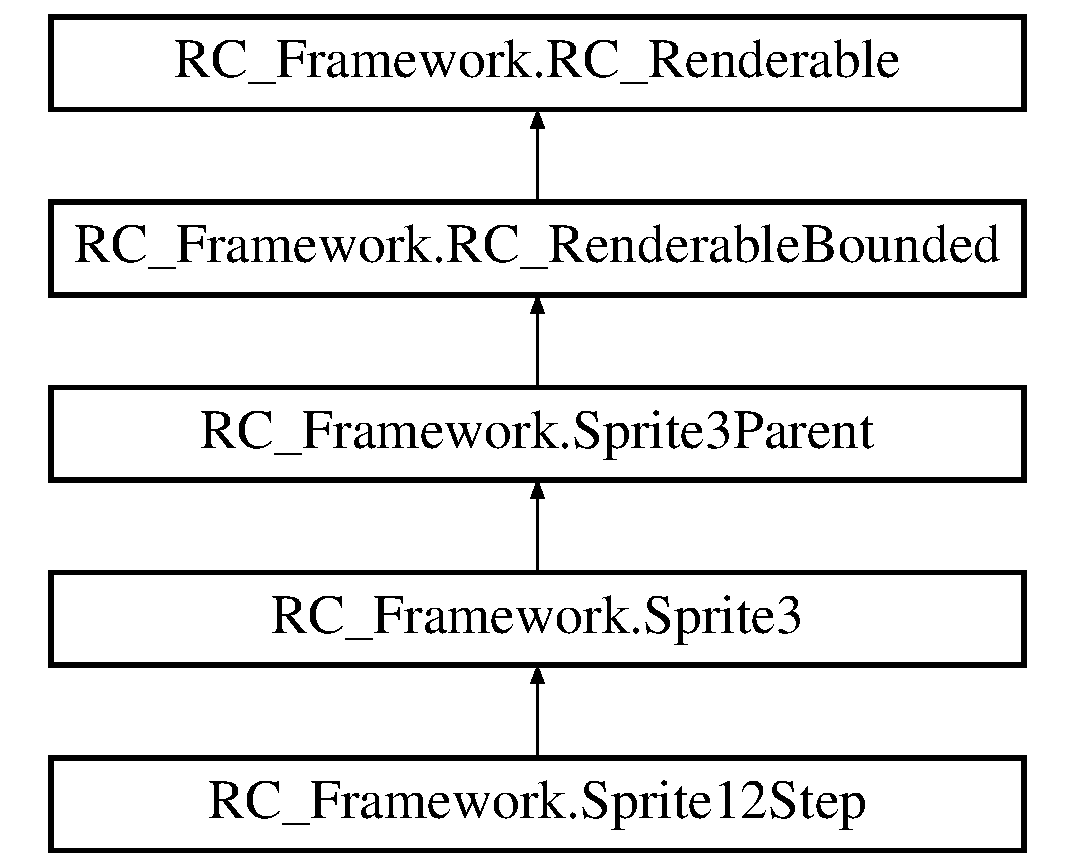
\includegraphics[height=5.000000cm]{class_r_c___framework_1_1_sprite3_parent}
\end{center}
\end{figure}
\subsection*{Public Member Functions}
\begin{DoxyCompactItemize}
\item 
override void \mbox{\hyperlink{class_r_c___framework_1_1_sprite3_parent_aafe2f4e919b30044d02600942068d205}{set\+Pos}} (float x, float y)
\begin{DoxyCompactList}\small\item\em sets the sprite location (top left of image) \end{DoxyCompactList}\item 
void \mbox{\hyperlink{class_r_c___framework_1_1_sprite3_parent_a850bd371ac0c564f36f14e2bf3ada72e}{set\+Pos}} (Vector2 p)
\begin{DoxyCompactList}\small\item\em sets the sprite location -\/ ie its hotspot on the screen note the default hotspot is the top left of image \end{DoxyCompactList}\item 
void \mbox{\hyperlink{class_r_c___framework_1_1_sprite3_parent_ae8cc0fe44090f72c9c9f38826ba0bd3f}{set\+PosX}} (float x)
\begin{DoxyCompactList}\small\item\em sets the X sprite location -\/ ie its hotspot on the screen note the default hotspot is the top left of image \end{DoxyCompactList}\item 
void \mbox{\hyperlink{class_r_c___framework_1_1_sprite3_parent_aacc2ace291d75d78005ab8d3f837a1af}{set\+PosY}} (float y)
\begin{DoxyCompactList}\small\item\em sets the Y sprite location -\/ ie its hotspot on the screen note the default hotspot is the top left of image \end{DoxyCompactList}\item 
float \mbox{\hyperlink{class_r_c___framework_1_1_sprite3_parent_a78aeb4a281abcd3a5cc83fabb4d24a8e}{get\+PosX}} ()
\begin{DoxyCompactList}\small\item\em returns the xpos of the sprite \end{DoxyCompactList}\item 
float \mbox{\hyperlink{class_r_c___framework_1_1_sprite3_parent_afaa8c7fd07554b39dbf6757656cd9065}{get\+PosY}} ()
\begin{DoxyCompactList}\small\item\em returns the ypos of the sprite \end{DoxyCompactList}\item 
Vector2 \mbox{\hyperlink{class_r_c___framework_1_1_sprite3_parent_aabeda600912d35738cdb6de98a40282a}{get\+Pos}} ()
\begin{DoxyCompactList}\small\item\em returns the position of the sprite \end{DoxyCompactList}\item 
virtual void \mbox{\hyperlink{class_r_c___framework_1_1_sprite3_parent_ad67b46aec70ebe4a720dc4550108b8c1}{restore\+Position}} ()
\begin{DoxyCompactList}\small\item\em restore the current position note its virtual and overidden in \mbox{\hyperlink{class_r_c___framework_1_1_sprite3}{Sprite3}} \end{DoxyCompactList}\item 
virtual void \mbox{\hyperlink{class_r_c___framework_1_1_sprite3_parent_ad934c0f7664064c6ac89525bf06516fc}{save\+Position}} ()
\begin{DoxyCompactList}\small\item\em Save the current position note its virtual and overidden in \mbox{\hyperlink{class_r_c___framework_1_1_sprite3}{Sprite3}} \end{DoxyCompactList}\end{DoxyCompactItemize}
\subsection*{Public Attributes}
\begin{DoxyCompactItemize}
\item 
Vector2 \mbox{\hyperlink{class_r_c___framework_1_1_sprite3_parent_ade2887bc3eda096dd75498936daae484}{save\+Pos}}
\begin{DoxyCompactList}\small\item\em Set by calling save\+Position, and used in restore\+Position \end{DoxyCompactList}\item 
Vector2 \mbox{\hyperlink{class_r_c___framework_1_1_sprite3_parent_a81a19273a375b067b83c5e01909bc576}{old\+Pos}}
\begin{DoxyCompactList}\small\item\em the previous position it is updated if the \mbox{\hyperlink{class_r_c___framework_1_1_sprite3}{Sprite3}} movement systems are used and can be used to compute a display angle this is for you to use/set if you have your own movement system \end{DoxyCompactList}\end{DoxyCompactItemize}
\subsection*{Protected Attributes}
\begin{DoxyCompactItemize}
\item 
Rectangle \mbox{\hyperlink{class_r_c___framework_1_1_sprite3_parent_af4043faa686325df81a690475feed4d8}{bb}}
\begin{DoxyCompactList}\small\item\em Bounding Box rectange in source pixels x and y are offset from the H\+O\+T\+S\+P\+OT Warning if the hotspot is in the middle of the image/frame then x,y will be negative \end{DoxyCompactList}\item 
Vector2 \mbox{\hyperlink{class_r_c___framework_1_1_sprite3_parent_af83a86a2944aec373fe87a170f3d7e2c}{pos}}
\begin{DoxyCompactList}\small\item\em the sprites location \end{DoxyCompactList}\end{DoxyCompactItemize}
\subsection*{Additional Inherited Members}


\subsection{Member Function Documentation}
\mbox{\Hypertarget{class_r_c___framework_1_1_sprite3_parent_aabeda600912d35738cdb6de98a40282a}\label{class_r_c___framework_1_1_sprite3_parent_aabeda600912d35738cdb6de98a40282a}} 
\index{R\+C\+\_\+\+Framework\+::\+Sprite3\+Parent@{R\+C\+\_\+\+Framework\+::\+Sprite3\+Parent}!get\+Pos@{get\+Pos}}
\index{get\+Pos@{get\+Pos}!R\+C\+\_\+\+Framework\+::\+Sprite3\+Parent@{R\+C\+\_\+\+Framework\+::\+Sprite3\+Parent}}
\subsubsection{\texorpdfstring{get\+Pos()}{getPos()}}
{\footnotesize\ttfamily Vector2 R\+C\+\_\+\+Framework.\+Sprite3\+Parent.\+get\+Pos (\begin{DoxyParamCaption}{ }\end{DoxyParamCaption})}



returns the position of the sprite 

\begin{DoxyReturn}{Returns}

\end{DoxyReturn}
\mbox{\Hypertarget{class_r_c___framework_1_1_sprite3_parent_a78aeb4a281abcd3a5cc83fabb4d24a8e}\label{class_r_c___framework_1_1_sprite3_parent_a78aeb4a281abcd3a5cc83fabb4d24a8e}} 
\index{R\+C\+\_\+\+Framework\+::\+Sprite3\+Parent@{R\+C\+\_\+\+Framework\+::\+Sprite3\+Parent}!get\+PosX@{get\+PosX}}
\index{get\+PosX@{get\+PosX}!R\+C\+\_\+\+Framework\+::\+Sprite3\+Parent@{R\+C\+\_\+\+Framework\+::\+Sprite3\+Parent}}
\subsubsection{\texorpdfstring{get\+Pos\+X()}{getPosX()}}
{\footnotesize\ttfamily float R\+C\+\_\+\+Framework.\+Sprite3\+Parent.\+get\+PosX (\begin{DoxyParamCaption}{ }\end{DoxyParamCaption})}



returns the xpos of the sprite 

\begin{DoxyReturn}{Returns}

\end{DoxyReturn}
\mbox{\Hypertarget{class_r_c___framework_1_1_sprite3_parent_afaa8c7fd07554b39dbf6757656cd9065}\label{class_r_c___framework_1_1_sprite3_parent_afaa8c7fd07554b39dbf6757656cd9065}} 
\index{R\+C\+\_\+\+Framework\+::\+Sprite3\+Parent@{R\+C\+\_\+\+Framework\+::\+Sprite3\+Parent}!get\+PosY@{get\+PosY}}
\index{get\+PosY@{get\+PosY}!R\+C\+\_\+\+Framework\+::\+Sprite3\+Parent@{R\+C\+\_\+\+Framework\+::\+Sprite3\+Parent}}
\subsubsection{\texorpdfstring{get\+Pos\+Y()}{getPosY()}}
{\footnotesize\ttfamily float R\+C\+\_\+\+Framework.\+Sprite3\+Parent.\+get\+PosY (\begin{DoxyParamCaption}{ }\end{DoxyParamCaption})}



returns the ypos of the sprite 

\begin{DoxyReturn}{Returns}

\end{DoxyReturn}
\mbox{\Hypertarget{class_r_c___framework_1_1_sprite3_parent_ad67b46aec70ebe4a720dc4550108b8c1}\label{class_r_c___framework_1_1_sprite3_parent_ad67b46aec70ebe4a720dc4550108b8c1}} 
\index{R\+C\+\_\+\+Framework\+::\+Sprite3\+Parent@{R\+C\+\_\+\+Framework\+::\+Sprite3\+Parent}!restore\+Position@{restore\+Position}}
\index{restore\+Position@{restore\+Position}!R\+C\+\_\+\+Framework\+::\+Sprite3\+Parent@{R\+C\+\_\+\+Framework\+::\+Sprite3\+Parent}}
\subsubsection{\texorpdfstring{restore\+Position()}{restorePosition()}}
{\footnotesize\ttfamily virtual void R\+C\+\_\+\+Framework.\+Sprite3\+Parent.\+restore\+Position (\begin{DoxyParamCaption}{ }\end{DoxyParamCaption})\hspace{0.3cm}{\ttfamily [virtual]}}



restore the current position note its virtual and overidden in \mbox{\hyperlink{class_r_c___framework_1_1_sprite3}{Sprite3}} 



Reimplemented in \mbox{\hyperlink{class_r_c___framework_1_1_sprite3_a4ffc487d5c332dee276909dad3dba57a}{R\+C\+\_\+\+Framework.\+Sprite3}}.

\mbox{\Hypertarget{class_r_c___framework_1_1_sprite3_parent_ad934c0f7664064c6ac89525bf06516fc}\label{class_r_c___framework_1_1_sprite3_parent_ad934c0f7664064c6ac89525bf06516fc}} 
\index{R\+C\+\_\+\+Framework\+::\+Sprite3\+Parent@{R\+C\+\_\+\+Framework\+::\+Sprite3\+Parent}!save\+Position@{save\+Position}}
\index{save\+Position@{save\+Position}!R\+C\+\_\+\+Framework\+::\+Sprite3\+Parent@{R\+C\+\_\+\+Framework\+::\+Sprite3\+Parent}}
\subsubsection{\texorpdfstring{save\+Position()}{savePosition()}}
{\footnotesize\ttfamily virtual void R\+C\+\_\+\+Framework.\+Sprite3\+Parent.\+save\+Position (\begin{DoxyParamCaption}{ }\end{DoxyParamCaption})\hspace{0.3cm}{\ttfamily [virtual]}}



Save the current position note its virtual and overidden in \mbox{\hyperlink{class_r_c___framework_1_1_sprite3}{Sprite3}} 



Reimplemented in \mbox{\hyperlink{class_r_c___framework_1_1_sprite3_ae4733340c18c8098b250418081020c6a}{R\+C\+\_\+\+Framework.\+Sprite3}}.

\mbox{\Hypertarget{class_r_c___framework_1_1_sprite3_parent_aafe2f4e919b30044d02600942068d205}\label{class_r_c___framework_1_1_sprite3_parent_aafe2f4e919b30044d02600942068d205}} 
\index{R\+C\+\_\+\+Framework\+::\+Sprite3\+Parent@{R\+C\+\_\+\+Framework\+::\+Sprite3\+Parent}!set\+Pos@{set\+Pos}}
\index{set\+Pos@{set\+Pos}!R\+C\+\_\+\+Framework\+::\+Sprite3\+Parent@{R\+C\+\_\+\+Framework\+::\+Sprite3\+Parent}}
\subsubsection{\texorpdfstring{set\+Pos()}{setPos()}\hspace{0.1cm}{\footnotesize\ttfamily [1/2]}}
{\footnotesize\ttfamily override void R\+C\+\_\+\+Framework.\+Sprite3\+Parent.\+set\+Pos (\begin{DoxyParamCaption}\item[{float}]{x,  }\item[{float}]{y }\end{DoxyParamCaption})\hspace{0.3cm}{\ttfamily [virtual]}}



sets the sprite location (top left of image) 


\begin{DoxyParams}{Parameters}
{\em x} & \\
\hline
{\em y} & \\
\hline
\end{DoxyParams}


Reimplemented from \mbox{\hyperlink{class_r_c___framework_1_1_r_c___renderable_bounded_a49d38185d66bf150677aaf9cc35eb4fa}{R\+C\+\_\+\+Framework.\+R\+C\+\_\+\+Renderable\+Bounded}}.

\mbox{\Hypertarget{class_r_c___framework_1_1_sprite3_parent_a850bd371ac0c564f36f14e2bf3ada72e}\label{class_r_c___framework_1_1_sprite3_parent_a850bd371ac0c564f36f14e2bf3ada72e}} 
\index{R\+C\+\_\+\+Framework\+::\+Sprite3\+Parent@{R\+C\+\_\+\+Framework\+::\+Sprite3\+Parent}!set\+Pos@{set\+Pos}}
\index{set\+Pos@{set\+Pos}!R\+C\+\_\+\+Framework\+::\+Sprite3\+Parent@{R\+C\+\_\+\+Framework\+::\+Sprite3\+Parent}}
\subsubsection{\texorpdfstring{set\+Pos()}{setPos()}\hspace{0.1cm}{\footnotesize\ttfamily [2/2]}}
{\footnotesize\ttfamily void R\+C\+\_\+\+Framework.\+Sprite3\+Parent.\+set\+Pos (\begin{DoxyParamCaption}\item[{Vector2}]{p }\end{DoxyParamCaption})}



sets the sprite location -\/ ie its hotspot on the screen note the default hotspot is the top left of image 


\begin{DoxyParams}{Parameters}
{\em p} & \\
\hline
\end{DoxyParams}
\mbox{\Hypertarget{class_r_c___framework_1_1_sprite3_parent_ae8cc0fe44090f72c9c9f38826ba0bd3f}\label{class_r_c___framework_1_1_sprite3_parent_ae8cc0fe44090f72c9c9f38826ba0bd3f}} 
\index{R\+C\+\_\+\+Framework\+::\+Sprite3\+Parent@{R\+C\+\_\+\+Framework\+::\+Sprite3\+Parent}!set\+PosX@{set\+PosX}}
\index{set\+PosX@{set\+PosX}!R\+C\+\_\+\+Framework\+::\+Sprite3\+Parent@{R\+C\+\_\+\+Framework\+::\+Sprite3\+Parent}}
\subsubsection{\texorpdfstring{set\+Pos\+X()}{setPosX()}}
{\footnotesize\ttfamily void R\+C\+\_\+\+Framework.\+Sprite3\+Parent.\+set\+PosX (\begin{DoxyParamCaption}\item[{float}]{x }\end{DoxyParamCaption})}



sets the X sprite location -\/ ie its hotspot on the screen note the default hotspot is the top left of image 


\begin{DoxyParams}{Parameters}
{\em x} & \\
\hline
\end{DoxyParams}
\mbox{\Hypertarget{class_r_c___framework_1_1_sprite3_parent_aacc2ace291d75d78005ab8d3f837a1af}\label{class_r_c___framework_1_1_sprite3_parent_aacc2ace291d75d78005ab8d3f837a1af}} 
\index{R\+C\+\_\+\+Framework\+::\+Sprite3\+Parent@{R\+C\+\_\+\+Framework\+::\+Sprite3\+Parent}!set\+PosY@{set\+PosY}}
\index{set\+PosY@{set\+PosY}!R\+C\+\_\+\+Framework\+::\+Sprite3\+Parent@{R\+C\+\_\+\+Framework\+::\+Sprite3\+Parent}}
\subsubsection{\texorpdfstring{set\+Pos\+Y()}{setPosY()}}
{\footnotesize\ttfamily void R\+C\+\_\+\+Framework.\+Sprite3\+Parent.\+set\+PosY (\begin{DoxyParamCaption}\item[{float}]{y }\end{DoxyParamCaption})}



sets the Y sprite location -\/ ie its hotspot on the screen note the default hotspot is the top left of image 


\begin{DoxyParams}{Parameters}
{\em y} & \\
\hline
\end{DoxyParams}


\subsection{Member Data Documentation}
\mbox{\Hypertarget{class_r_c___framework_1_1_sprite3_parent_af4043faa686325df81a690475feed4d8}\label{class_r_c___framework_1_1_sprite3_parent_af4043faa686325df81a690475feed4d8}} 
\index{R\+C\+\_\+\+Framework\+::\+Sprite3\+Parent@{R\+C\+\_\+\+Framework\+::\+Sprite3\+Parent}!bb@{bb}}
\index{bb@{bb}!R\+C\+\_\+\+Framework\+::\+Sprite3\+Parent@{R\+C\+\_\+\+Framework\+::\+Sprite3\+Parent}}
\subsubsection{\texorpdfstring{bb}{bb}}
{\footnotesize\ttfamily Rectangle R\+C\+\_\+\+Framework.\+Sprite3\+Parent.\+bb\hspace{0.3cm}{\ttfamily [protected]}}



Bounding Box rectange in source pixels x and y are offset from the H\+O\+T\+S\+P\+OT Warning if the hotspot is in the middle of the image/frame then x,y will be negative 

\mbox{\Hypertarget{class_r_c___framework_1_1_sprite3_parent_a81a19273a375b067b83c5e01909bc576}\label{class_r_c___framework_1_1_sprite3_parent_a81a19273a375b067b83c5e01909bc576}} 
\index{R\+C\+\_\+\+Framework\+::\+Sprite3\+Parent@{R\+C\+\_\+\+Framework\+::\+Sprite3\+Parent}!old\+Pos@{old\+Pos}}
\index{old\+Pos@{old\+Pos}!R\+C\+\_\+\+Framework\+::\+Sprite3\+Parent@{R\+C\+\_\+\+Framework\+::\+Sprite3\+Parent}}
\subsubsection{\texorpdfstring{old\+Pos}{oldPos}}
{\footnotesize\ttfamily Vector2 R\+C\+\_\+\+Framework.\+Sprite3\+Parent.\+old\+Pos}



the previous position it is updated if the \mbox{\hyperlink{class_r_c___framework_1_1_sprite3}{Sprite3}} movement systems are used and can be used to compute a display angle this is for you to use/set if you have your own movement system 

\mbox{\Hypertarget{class_r_c___framework_1_1_sprite3_parent_af83a86a2944aec373fe87a170f3d7e2c}\label{class_r_c___framework_1_1_sprite3_parent_af83a86a2944aec373fe87a170f3d7e2c}} 
\index{R\+C\+\_\+\+Framework\+::\+Sprite3\+Parent@{R\+C\+\_\+\+Framework\+::\+Sprite3\+Parent}!pos@{pos}}
\index{pos@{pos}!R\+C\+\_\+\+Framework\+::\+Sprite3\+Parent@{R\+C\+\_\+\+Framework\+::\+Sprite3\+Parent}}
\subsubsection{\texorpdfstring{pos}{pos}}
{\footnotesize\ttfamily Vector2 R\+C\+\_\+\+Framework.\+Sprite3\+Parent.\+pos\hspace{0.3cm}{\ttfamily [protected]}}



the sprites location 

\mbox{\Hypertarget{class_r_c___framework_1_1_sprite3_parent_ade2887bc3eda096dd75498936daae484}\label{class_r_c___framework_1_1_sprite3_parent_ade2887bc3eda096dd75498936daae484}} 
\index{R\+C\+\_\+\+Framework\+::\+Sprite3\+Parent@{R\+C\+\_\+\+Framework\+::\+Sprite3\+Parent}!save\+Pos@{save\+Pos}}
\index{save\+Pos@{save\+Pos}!R\+C\+\_\+\+Framework\+::\+Sprite3\+Parent@{R\+C\+\_\+\+Framework\+::\+Sprite3\+Parent}}
\subsubsection{\texorpdfstring{save\+Pos}{savePos}}
{\footnotesize\ttfamily Vector2 R\+C\+\_\+\+Framework.\+Sprite3\+Parent.\+save\+Pos}



Set by calling save\+Position, and used in restore\+Position 



The documentation for this class was generated from the following file\+:\begin{DoxyCompactItemize}
\item 
F\+:/\+B/\+R\+C\+\_\+\+Framework2018/\+Source/\mbox{\hyperlink{_r_c___sprite3_8cs}{R\+C\+\_\+\+Sprite3.\+cs}}\end{DoxyCompactItemize}

\hypertarget{class_r_c___framework_1_1_sprite_factory_parent}{}\section{R\+C\+\_\+\+Framework.\+Sprite\+Factory\+Parent Class Reference}
\label{class_r_c___framework_1_1_sprite_factory_parent}\index{R\+C\+\_\+\+Framework.\+Sprite\+Factory\+Parent@{R\+C\+\_\+\+Framework.\+Sprite\+Factory\+Parent}}


This is a parent class for classes that create sprites -\/ generators and such  


Inheritance diagram for R\+C\+\_\+\+Framework.\+Sprite\+Factory\+Parent\+:\begin{figure}[H]
\begin{center}
\leavevmode
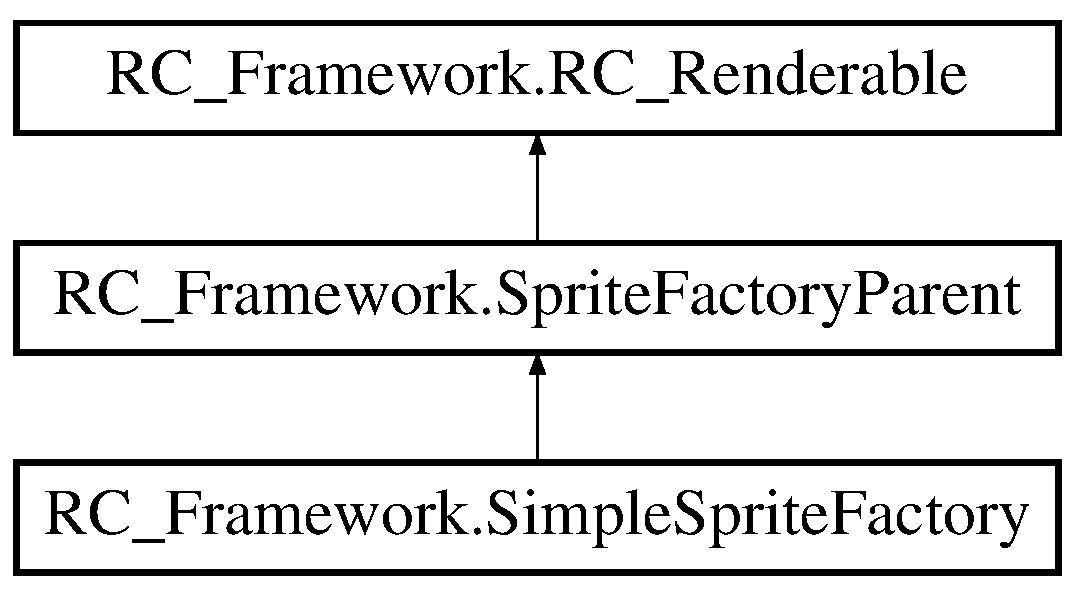
\includegraphics[height=3.000000cm]{class_r_c___framework_1_1_sprite_factory_parent}
\end{center}
\end{figure}
\subsection*{Public Member Functions}
\begin{DoxyCompactItemize}
\item 
virtual \mbox{\hyperlink{class_r_c___framework_1_1_sprite3}{Sprite3}} \mbox{\hyperlink{class_r_c___framework_1_1_sprite_factory_parent_a08e256b352d7f8042e9ee9d76206660d}{generate}} (int kind, int param)
\begin{DoxyCompactList}\small\item\em Generate a sprite kind and param is optionnal \end{DoxyCompactList}\item 
virtual \mbox{\hyperlink{class_r_c___framework_1_1_sprite3}{Sprite3}} \mbox{\hyperlink{class_r_c___framework_1_1_sprite_factory_parent_a81880f021af6b5ebe905b92a818cec07}{generate}} (Rectangle boundz)
\begin{DoxyCompactList}\small\item\em Just give it a position \end{DoxyCompactList}\item 
virtual \mbox{\hyperlink{class_r_c___framework_1_1_sprite3}{Sprite3}} \mbox{\hyperlink{class_r_c___framework_1_1_sprite_factory_parent_a0149ef937b4d172caf252112939fafa2}{generate}} ()
\begin{DoxyCompactList}\small\item\em Generate a sprite kind and param is optionnal \end{DoxyCompactList}\item 
abstract \mbox{\hyperlink{class_r_c___framework_1_1_sprite3}{Sprite3}} \mbox{\hyperlink{class_r_c___framework_1_1_sprite_factory_parent_ace3d0e7a00dd88a16a652ed5fa6a90bd}{generate\+At}} (int kind, int param, Rectangle boundz)
\begin{DoxyCompactList}\small\item\em generate sprite with all parametrs \end{DoxyCompactList}\end{DoxyCompactItemize}
\subsection*{Additional Inherited Members}


\subsection{Detailed Description}
This is a parent class for classes that create sprites -\/ generators and such 



\subsection{Member Function Documentation}
\mbox{\Hypertarget{class_r_c___framework_1_1_sprite_factory_parent_a08e256b352d7f8042e9ee9d76206660d}\label{class_r_c___framework_1_1_sprite_factory_parent_a08e256b352d7f8042e9ee9d76206660d}} 
\index{R\+C\+\_\+\+Framework\+::\+Sprite\+Factory\+Parent@{R\+C\+\_\+\+Framework\+::\+Sprite\+Factory\+Parent}!generate@{generate}}
\index{generate@{generate}!R\+C\+\_\+\+Framework\+::\+Sprite\+Factory\+Parent@{R\+C\+\_\+\+Framework\+::\+Sprite\+Factory\+Parent}}
\subsubsection{\texorpdfstring{generate()}{generate()}\hspace{0.1cm}{\footnotesize\ttfamily [1/3]}}
{\footnotesize\ttfamily virtual \mbox{\hyperlink{class_r_c___framework_1_1_sprite3}{Sprite3}} R\+C\+\_\+\+Framework.\+Sprite\+Factory\+Parent.\+generate (\begin{DoxyParamCaption}\item[{int}]{kind,  }\item[{int}]{param }\end{DoxyParamCaption})\hspace{0.3cm}{\ttfamily [virtual]}}



Generate a sprite kind and param is optionnal 


\begin{DoxyParams}{Parameters}
{\em kind} & \\
\hline
{\em param} & \\
\hline
\end{DoxyParams}
\begin{DoxyReturn}{Returns}

\end{DoxyReturn}
\mbox{\Hypertarget{class_r_c___framework_1_1_sprite_factory_parent_a81880f021af6b5ebe905b92a818cec07}\label{class_r_c___framework_1_1_sprite_factory_parent_a81880f021af6b5ebe905b92a818cec07}} 
\index{R\+C\+\_\+\+Framework\+::\+Sprite\+Factory\+Parent@{R\+C\+\_\+\+Framework\+::\+Sprite\+Factory\+Parent}!generate@{generate}}
\index{generate@{generate}!R\+C\+\_\+\+Framework\+::\+Sprite\+Factory\+Parent@{R\+C\+\_\+\+Framework\+::\+Sprite\+Factory\+Parent}}
\subsubsection{\texorpdfstring{generate()}{generate()}\hspace{0.1cm}{\footnotesize\ttfamily [2/3]}}
{\footnotesize\ttfamily virtual \mbox{\hyperlink{class_r_c___framework_1_1_sprite3}{Sprite3}} R\+C\+\_\+\+Framework.\+Sprite\+Factory\+Parent.\+generate (\begin{DoxyParamCaption}\item[{Rectangle}]{boundz }\end{DoxyParamCaption})\hspace{0.3cm}{\ttfamily [virtual]}}



Just give it a position 


\begin{DoxyParams}{Parameters}
{\em kind} & \\
\hline
{\em param} & \\
\hline
\end{DoxyParams}
\begin{DoxyReturn}{Returns}

\end{DoxyReturn}
\mbox{\Hypertarget{class_r_c___framework_1_1_sprite_factory_parent_a0149ef937b4d172caf252112939fafa2}\label{class_r_c___framework_1_1_sprite_factory_parent_a0149ef937b4d172caf252112939fafa2}} 
\index{R\+C\+\_\+\+Framework\+::\+Sprite\+Factory\+Parent@{R\+C\+\_\+\+Framework\+::\+Sprite\+Factory\+Parent}!generate@{generate}}
\index{generate@{generate}!R\+C\+\_\+\+Framework\+::\+Sprite\+Factory\+Parent@{R\+C\+\_\+\+Framework\+::\+Sprite\+Factory\+Parent}}
\subsubsection{\texorpdfstring{generate()}{generate()}\hspace{0.1cm}{\footnotesize\ttfamily [3/3]}}
{\footnotesize\ttfamily virtual \mbox{\hyperlink{class_r_c___framework_1_1_sprite3}{Sprite3}} R\+C\+\_\+\+Framework.\+Sprite\+Factory\+Parent.\+generate (\begin{DoxyParamCaption}{ }\end{DoxyParamCaption})\hspace{0.3cm}{\ttfamily [virtual]}}



Generate a sprite kind and param is optionnal 

\begin{DoxyReturn}{Returns}

\end{DoxyReturn}
\mbox{\Hypertarget{class_r_c___framework_1_1_sprite_factory_parent_ace3d0e7a00dd88a16a652ed5fa6a90bd}\label{class_r_c___framework_1_1_sprite_factory_parent_ace3d0e7a00dd88a16a652ed5fa6a90bd}} 
\index{R\+C\+\_\+\+Framework\+::\+Sprite\+Factory\+Parent@{R\+C\+\_\+\+Framework\+::\+Sprite\+Factory\+Parent}!generate\+At@{generate\+At}}
\index{generate\+At@{generate\+At}!R\+C\+\_\+\+Framework\+::\+Sprite\+Factory\+Parent@{R\+C\+\_\+\+Framework\+::\+Sprite\+Factory\+Parent}}
\subsubsection{\texorpdfstring{generate\+At()}{generateAt()}}
{\footnotesize\ttfamily abstract \mbox{\hyperlink{class_r_c___framework_1_1_sprite3}{Sprite3}} R\+C\+\_\+\+Framework.\+Sprite\+Factory\+Parent.\+generate\+At (\begin{DoxyParamCaption}\item[{int}]{kind,  }\item[{int}]{param,  }\item[{Rectangle}]{boundz }\end{DoxyParamCaption})\hspace{0.3cm}{\ttfamily [pure virtual]}}



generate sprite with all parametrs 


\begin{DoxyParams}{Parameters}
{\em x} & \\
\hline
{\em y} & \\
\hline
{\em width} & \\
\hline
{\em heigth} & \\
\hline
\end{DoxyParams}
\begin{DoxyReturn}{Returns}

\end{DoxyReturn}


Implemented in \mbox{\hyperlink{class_r_c___framework_1_1_simple_sprite_factory_ab008431fcc3f967b70de9a155d1a529a}{R\+C\+\_\+\+Framework.\+Simple\+Sprite\+Factory}}.



The documentation for this class was generated from the following file\+:\begin{DoxyCompactItemize}
\item 
F\+:/\+B/\+R\+C\+\_\+\+Framework2018/\+Source/\mbox{\hyperlink{_r_c___sprite3_8cs}{R\+C\+\_\+\+Sprite3.\+cs}}\end{DoxyCompactItemize}

\hypertarget{class_r_c___framework_1_1_sprite_list}{}\section{R\+C\+\_\+\+Framework.\+Sprite\+List Class Reference}
\label{class_r_c___framework_1_1_sprite_list}\index{R\+C\+\_\+\+Framework.\+Sprite\+List@{R\+C\+\_\+\+Framework.\+Sprite\+List}}


A list of sprites with some basic management functions It has the concept than sprites are visbile or not visible and active or not active the function addspritereuse -\/ reuses the inactive sprite slots  


Inheritance diagram for R\+C\+\_\+\+Framework.\+Sprite\+List\+:\begin{figure}[H]
\begin{center}
\leavevmode
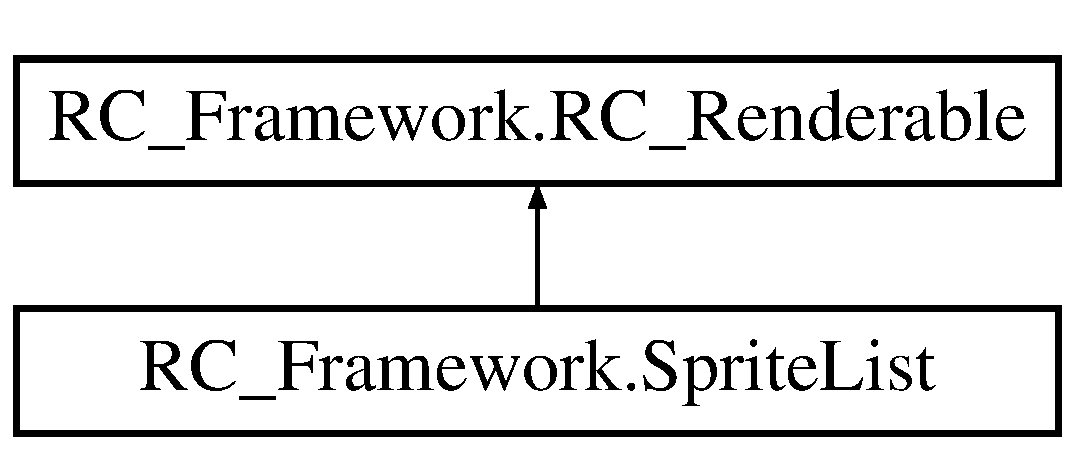
\includegraphics[height=2.000000cm]{class_r_c___framework_1_1_sprite_list}
\end{center}
\end{figure}
\subsection*{Public Member Functions}
\begin{DoxyCompactItemize}
\item 
\mbox{\hyperlink{class_r_c___framework_1_1_sprite_list_aa12cce855c8cfefbfb9dd4f011ee6b0c}{Sprite\+List}} ()
\begin{DoxyCompactList}\small\item\em Constructor for spritelist \end{DoxyCompactList}\item 
\mbox{\hyperlink{class_r_c___framework_1_1_sprite_list_ab960d5ea8bbf16fe40562fc083ce8059}{Sprite\+List}} (int Num\+Of\+Sprites)
\begin{DoxyCompactList}\small\item\em Constructor if you want to manage how many sprites \end{DoxyCompactList}\item 
int \mbox{\hyperlink{class_r_c___framework_1_1_sprite_list_a5ae9a1c4902704af27642541288eab22}{count}} ()
\begin{DoxyCompactList}\small\item\em counts sprites in list (active, inactive , visible, not visible) fairly useless \end{DoxyCompactList}\item 
int \mbox{\hyperlink{class_r_c___framework_1_1_sprite_list_a806056c18832f13d2adf0dad0c0b2152}{count\+Active}} ()
\begin{DoxyCompactList}\small\item\em counts sprites in list (active only) \end{DoxyCompactList}\item 
int \mbox{\hyperlink{class_r_c___framework_1_1_sprite_list_a093cf170b2802f89be43bf86ed81662e}{get\+Max\+Num\+Of\+Sprites}} ()
\begin{DoxyCompactList}\small\item\em Get max number of sprites in this list \end{DoxyCompactList}\item 
int \mbox{\hyperlink{class_r_c___framework_1_1_sprite_list_aad3ba75650382840c4c11d28022bc288}{get\+Highest\+Used}} ()
\begin{DoxyCompactList}\small\item\em get the index of the highest used sprite \end{DoxyCompactList}\item 
int \mbox{\hyperlink{class_r_c___framework_1_1_sprite_list_a3d07b6b3927153b2dec5f13666908cfe}{find\+Free\+Sprite}} ()
\begin{DoxyCompactList}\small\item\em Finds a free slot in the sprite list or -\/1 if it fails \end{DoxyCompactList}\item 
int \mbox{\hyperlink{class_r_c___framework_1_1_sprite_list_a019afbeb0e8e39bbc9e5a5c6cf34f777}{find\+Free\+Sprite\+Or\+Inactive}} ()
\begin{DoxyCompactList}\small\item\em Finds a free slot in the sprite list or an inactive sprite -\/1 if it fails \end{DoxyCompactList}\item 
int \mbox{\hyperlink{class_r_c___framework_1_1_sprite_list_a8f45da7ee7263d6f9167a2961e14a412}{add\+Sprite}} (\mbox{\hyperlink{class_r_c___framework_1_1_sprite3}{Sprite3}} spriteZ)
\begin{DoxyCompactList}\small\item\em Add a sprite and return then return the number we added it at return -\/1 if not possible \end{DoxyCompactList}\item 
int \mbox{\hyperlink{class_r_c___framework_1_1_sprite_list_a0ff2817bd891443dd588b37aad792cf0}{add\+Sprite\+Reuse}} (\mbox{\hyperlink{class_r_c___framework_1_1_sprite3}{Sprite3}} spriteZ)
\begin{DoxyCompactList}\small\item\em Add a sprite and return then number we added it at and allow inactive sprites to be oever written return -\/1 if not possible \end{DoxyCompactList}\item 
\mbox{\hyperlink{class_r_c___framework_1_1_sprite3}{Sprite3}} \mbox{\hyperlink{class_r_c___framework_1_1_sprite_list_a430b89d680a7267307b61d7cb81d948d}{get\+Sprite}} (int i)
\begin{DoxyCompactList}\small\item\em return the particular sprite \end{DoxyCompactList}\item 
void \mbox{\hyperlink{class_r_c___framework_1_1_sprite_list_a6976b2d2feaf72f41d92a8981e595efb}{delete\+Sprite}} (int i)
\begin{DoxyCompactList}\small\item\em Remove a sprite \end{DoxyCompactList}\item 
void \mbox{\hyperlink{class_r_c___framework_1_1_sprite_list_a9ddabec41f012b498c09368318c1941c}{set\+Sprite}} (int i, \mbox{\hyperlink{class_r_c___framework_1_1_sprite3}{Sprite3}} spriteZ)
\begin{DoxyCompactList}\small\item\em Replace or set a specifically numbered sprite \end{DoxyCompactList}\item 
override void \mbox{\hyperlink{class_r_c___framework_1_1_sprite_list_a4100c8d4abaa1e7268c17607d70b539a}{Draw}} (Sprite\+Batch sb)
\begin{DoxyCompactList}\small\item\em draw all visible sprites \end{DoxyCompactList}\item 
void \mbox{\hyperlink{class_r_c___framework_1_1_sprite_list_aab5a80e0d7a8340768db890a9af8a90c}{draw\+All}} (Sprite\+Batch sb)
\begin{DoxyCompactList}\small\item\em draw all visible and active sprites \end{DoxyCompactList}\item 
void \mbox{\hyperlink{class_r_c___framework_1_1_sprite_list_a501e6bd0f2a0910e5259db8189e23ce4}{animation\+Tick}} (Game\+Time game\+Time)
\begin{DoxyCompactList}\small\item\em animation\+Tick tick all visible and active sprites \end{DoxyCompactList}\item 
void \mbox{\hyperlink{class_r_c___framework_1_1_sprite_list_af36a07386a5b0f32a74473890868b3fc}{Tick}} ()
\begin{DoxyCompactList}\small\item\em Run routine tick on all active sprites -\/ this may alter their visiblity or active staus Tick is used in sprite3 to make a sprite visible after a certain time \end{DoxyCompactList}\item 
override void \mbox{\hyperlink{class_r_c___framework_1_1_sprite_list_aba7adceacb386357f811b5099d8885ca}{set\+Color}} (Color c)
\begin{DoxyCompactList}\small\item\em Run set\+Color on all active sprites \end{DoxyCompactList}\item 
override void \mbox{\hyperlink{class_r_c___framework_1_1_sprite_list_a816100deff7ad173c33904ac59f3ad79}{Update}} (Game\+Time game\+Time)
\begin{DoxyCompactList}\small\item\em Run Update on all active sprites; but most of the time you actually want one of (or more of)\+: \end{DoxyCompactList}\item 
void \mbox{\hyperlink{class_r_c___framework_1_1_sprite_list_a865a310d536bf2fd0b23f01b84159887}{draw\+Active}} (Sprite\+Batch sb)
\begin{DoxyCompactList}\small\item\em Draw all active sprites \end{DoxyCompactList}\item 
void \mbox{\hyperlink{class_r_c___framework_1_1_sprite_list_a5467136da9d231b4e99444adb5f52470}{move\+By\+Angle\+Speed}} ()
\begin{DoxyCompactList}\small\item\em Calls \mbox{\hyperlink{class_r_c___framework_1_1_sprite_list_a5467136da9d231b4e99444adb5f52470}{move\+By\+Angle\+Speed()}}; on all active sprites in the list \end{DoxyCompactList}\item 
void \mbox{\hyperlink{class_r_c___framework_1_1_sprite_list_a9d1b368c9d6d8e340e66faa06c63e5dd}{move\+Active\+AD}} ()
\begin{DoxyCompactList}\small\item\em Move active by angle/dist \end{DoxyCompactList}\item 
void \mbox{\hyperlink{class_r_c___framework_1_1_sprite_list_a1ad88a094e1efbdd75de18f8f1d49db1}{move\+By\+Angle\+Speeed\+Limit}} (Rectangle r)
\begin{DoxyCompactList}\small\item\em runs move\+By\+Angle\+Speeed\+Limit on all active sprites \end{DoxyCompactList}\item 
void \mbox{\hyperlink{class_r_c___framework_1_1_sprite_list_a91c1c36f7a1b321e6a1351fddd9c7e3e}{adjust\+Angles}} ()
\begin{DoxyCompactList}\small\item\em Adjust all angles (move and display) by relevant deltas \end{DoxyCompactList}\item 
void \mbox{\hyperlink{class_r_c___framework_1_1_sprite_list_a0d85e7ec742d8326291f6d51ab0e0b0e}{adjust\+Angles\+Active}} ()
\begin{DoxyCompactList}\small\item\em Adjust all angles (move and display) by relevant deltas \end{DoxyCompactList}\item 
int \mbox{\hyperlink{class_r_c___framework_1_1_sprite_list_a993e1c122878810e0e4cb439bc34be45}{remove\+If\+Outside}} (Rectangle r)
\begin{DoxyCompactList}\small\item\em Removes (makes inactive) all sprites whos bouding vbox is outside r returns a count of the number of sprites removed \end{DoxyCompactList}\item 
void \mbox{\hyperlink{class_r_c___framework_1_1_sprite_list_a61d8b26102baae989a9a9c82b1242c0c}{move\+Delta\+X\+Y\+\_\+\+Visible}} ()
\begin{DoxyCompactList}\small\item\em Move visible or active by delat x delta y \end{DoxyCompactList}\item 
void \mbox{\hyperlink{class_r_c___framework_1_1_sprite_list_a7412f51e494ab844da5c81c24d1b24a9}{move\+Delta\+XY}} ()
\begin{DoxyCompactList}\small\item\em Move active by delta x delta y \end{DoxyCompactList}\item 
override bool \mbox{\hyperlink{class_r_c___framework_1_1_sprite_list_ac4dbeb822b300bdcbebeb20c15b7bc9a}{scroll\+Move}} (float x, float y)
\begin{DoxyCompactList}\small\item\em Call scrollmove to move all sprites \end{DoxyCompactList}\item 
void \mbox{\hyperlink{class_r_c___framework_1_1_sprite_list_ab65f3d6bc7574e4b5df5c36b09d4d0b7}{move\+DeltaX}} (float dx)
\begin{DoxyCompactList}\small\item\em Move active by a delta x \end{DoxyCompactList}\item 
void \mbox{\hyperlink{class_r_c___framework_1_1_sprite_list_a49e91f6101d88d31069bb76d76efe9af}{move\+DeltaY}} (float dy)
\begin{DoxyCompactList}\small\item\em Move active by a delta y \end{DoxyCompactList}\item 
void \mbox{\hyperlink{class_r_c___framework_1_1_sprite_list_a2f4c60ffbdb1ed918079bb2572b0dcf5}{move\+Visible\+Way\+Points}} ()
\begin{DoxyCompactList}\small\item\em Move all active visible sprites by their waypoint \end{DoxyCompactList}\item 
void \mbox{\hyperlink{class_r_c___framework_1_1_sprite_list_a172fdc75116eeac16731188b46b7dac6}{draw\+Info}} (Sprite\+Batch sb, Color color\+BB, Color color\+HS)
\begin{DoxyCompactList}\small\item\em Draw BB and hotspot for all visible sprites \end{DoxyCompactList}\item 
void \mbox{\hyperlink{class_r_c___framework_1_1_sprite_list_a3927cc35567aca5b96ebd966a8b480be}{draw\+Bounding\+Sphere}} (Sprite\+Batch sb, Color color\+BS)
\begin{DoxyCompactList}\small\item\em draw Bounding Spheres in list \end{DoxyCompactList}\item 
void \mbox{\hyperlink{class_r_c___framework_1_1_sprite_list_af03b9a1d139cffcaa9cb32170788998e}{draw\+Way\+Lists}} (Sprite\+Batch sb, Color colorW)
\begin{DoxyCompactList}\small\item\em Draw the waypoints \end{DoxyCompactList}\item 
void \mbox{\hyperlink{class_r_c___framework_1_1_sprite_list_adbb96b3d84627126045be2b406c9ab12}{draw\+Rect4}} (Sprite\+Batch sb, Color color)
\begin{DoxyCompactList}\small\item\em draws the rotated bounding box for all visible sprites \end{DoxyCompactList}\item 
int \mbox{\hyperlink{class_r_c___framework_1_1_sprite_list_a3cb2f1e0826f5a00623500c8f6e824e9}{collision\+AA}} (\mbox{\hyperlink{class_r_c___framework_1_1_sprite3}{Sprite3}} s)
\begin{DoxyCompactList}\small\item\em Returns the index of the first (ie lowest numbered) sprite it colides with -\/1 if no colission \end{DoxyCompactList}\item 
int \mbox{\hyperlink{class_r_c___framework_1_1_sprite_list_aae4b98d6d9acdf7c2b2160eb6a4189d8}{collision\+AA}} (\mbox{\hyperlink{class_r_c___framework_1_1_sprite3}{Sprite3}} s, int self)
\begin{DoxyCompactList}\small\item\em Returns the index of the first (ie lowest numbered) sprite it colides with -\/1 if no collision the self parameter is there to allow the avoidance of collision texting against yourself \end{DoxyCompactList}\item 
int \mbox{\hyperlink{class_r_c___framework_1_1_sprite_list_ac5d904b4fb5a97aadefde7838aea186c}{collision\+With\+Rect}} (Rectangle r)
\begin{DoxyCompactList}\small\item\em returns index of the first visible sprite that collides with r if no colission it returns -\/1 \end{DoxyCompactList}\item 
int \mbox{\hyperlink{class_r_c___framework_1_1_sprite_list_a06ea4d7accd25d0fb593bcf043bb16b5}{point\+In\+List}} (Vector2 point)
\begin{DoxyCompactList}\small\item\em Returns the number of the first sprite found \textquotesingle{}under\textquotesingle{} the spot \end{DoxyCompactList}\item 
int \mbox{\hyperlink{class_r_c___framework_1_1_sprite_list_a737c9d5cc39dbb8c3754b2fd6d67e8ab}{find\+Inactive}} ()
\begin{DoxyCompactList}\small\item\em Find inactive sprite or -\/1 if not found \end{DoxyCompactList}\item 
bool \mbox{\hyperlink{class_r_c___framework_1_1_sprite_list_ad3406b2aeba1b08f23f13a35454f63e3}{Run\+The\+Method}} (Func$<$ \mbox{\hyperlink{class_r_c___framework_1_1_sprite3}{Sprite3}}, bool $>$ method\+Name)
\begin{DoxyCompactList}\small\item\em Run the method on each active sprite return true only if all functions return true (or possibly there were no active sprites) the function has the formal parameters bool name(\+Sprite3 s) \end{DoxyCompactList}\end{DoxyCompactItemize}
\subsection*{Public Attributes}
\begin{DoxyCompactItemize}
\item 
int \mbox{\hyperlink{class_r_c___framework_1_1_sprite_list_ac5f0c7b4e89b70c3ca6d87c45d874ad9}{low\+Free}} = 0
\begin{DoxyCompactList}\small\item\em Lowest free sprite num (for use in external loops rarely needed) \end{DoxyCompactList}\item 
int \mbox{\hyperlink{class_r_c___framework_1_1_sprite_list_acba70858abae8afe358df8fe61c8c394}{high\+Used}} = 0
\begin{DoxyCompactList}\small\item\em Highest free sprite num (for use in external loops rarely needed) \end{DoxyCompactList}\end{DoxyCompactItemize}
\subsection*{Properties}
\begin{DoxyCompactItemize}
\item 
\mbox{\hyperlink{class_r_c___framework_1_1_sprite3}{Sprite3}} \mbox{\hyperlink{class_r_c___framework_1_1_sprite_list_ad32b304d8023b1a91a3021545436c4e5}{this\mbox{[}int key\mbox{]}}}\hspace{0.3cm}{\ttfamily  \mbox{[}get, set\mbox{]}}
\begin{DoxyCompactList}\small\item\em Overload \mbox{[} and \mbox{]} for ease of use \end{DoxyCompactList}\end{DoxyCompactItemize}


\subsection{Detailed Description}
A list of sprites with some basic management functions It has the concept than sprites are visbile or not visible and active or not active the function addspritereuse -\/ reuses the inactive sprite slots 



\subsection{Constructor \& Destructor Documentation}
\mbox{\Hypertarget{class_r_c___framework_1_1_sprite_list_aa12cce855c8cfefbfb9dd4f011ee6b0c}\label{class_r_c___framework_1_1_sprite_list_aa12cce855c8cfefbfb9dd4f011ee6b0c}} 
\index{R\+C\+\_\+\+Framework\+::\+Sprite\+List@{R\+C\+\_\+\+Framework\+::\+Sprite\+List}!Sprite\+List@{Sprite\+List}}
\index{Sprite\+List@{Sprite\+List}!R\+C\+\_\+\+Framework\+::\+Sprite\+List@{R\+C\+\_\+\+Framework\+::\+Sprite\+List}}
\subsubsection{\texorpdfstring{Sprite\+List()}{SpriteList()}\hspace{0.1cm}{\footnotesize\ttfamily [1/2]}}
{\footnotesize\ttfamily R\+C\+\_\+\+Framework.\+Sprite\+List.\+Sprite\+List (\begin{DoxyParamCaption}{ }\end{DoxyParamCaption})}



Constructor for spritelist 

\mbox{\Hypertarget{class_r_c___framework_1_1_sprite_list_ab960d5ea8bbf16fe40562fc083ce8059}\label{class_r_c___framework_1_1_sprite_list_ab960d5ea8bbf16fe40562fc083ce8059}} 
\index{R\+C\+\_\+\+Framework\+::\+Sprite\+List@{R\+C\+\_\+\+Framework\+::\+Sprite\+List}!Sprite\+List@{Sprite\+List}}
\index{Sprite\+List@{Sprite\+List}!R\+C\+\_\+\+Framework\+::\+Sprite\+List@{R\+C\+\_\+\+Framework\+::\+Sprite\+List}}
\subsubsection{\texorpdfstring{Sprite\+List()}{SpriteList()}\hspace{0.1cm}{\footnotesize\ttfamily [2/2]}}
{\footnotesize\ttfamily R\+C\+\_\+\+Framework.\+Sprite\+List.\+Sprite\+List (\begin{DoxyParamCaption}\item[{int}]{Num\+Of\+Sprites }\end{DoxyParamCaption})}



Constructor if you want to manage how many sprites 


\begin{DoxyParams}{Parameters}
{\em Num\+Of\+Sprites} & \\
\hline
\end{DoxyParams}


\subsection{Member Function Documentation}
\mbox{\Hypertarget{class_r_c___framework_1_1_sprite_list_a8f45da7ee7263d6f9167a2961e14a412}\label{class_r_c___framework_1_1_sprite_list_a8f45da7ee7263d6f9167a2961e14a412}} 
\index{R\+C\+\_\+\+Framework\+::\+Sprite\+List@{R\+C\+\_\+\+Framework\+::\+Sprite\+List}!add\+Sprite@{add\+Sprite}}
\index{add\+Sprite@{add\+Sprite}!R\+C\+\_\+\+Framework\+::\+Sprite\+List@{R\+C\+\_\+\+Framework\+::\+Sprite\+List}}
\subsubsection{\texorpdfstring{add\+Sprite()}{addSprite()}}
{\footnotesize\ttfamily int R\+C\+\_\+\+Framework.\+Sprite\+List.\+add\+Sprite (\begin{DoxyParamCaption}\item[{\mbox{\hyperlink{class_r_c___framework_1_1_sprite3}{Sprite3}}}]{spriteZ }\end{DoxyParamCaption})}



Add a sprite and return then return the number we added it at return -\/1 if not possible 


\begin{DoxyParams}{Parameters}
{\em spriteZ} & \\
\hline
\end{DoxyParams}
\begin{DoxyReturn}{Returns}

\end{DoxyReturn}
\mbox{\Hypertarget{class_r_c___framework_1_1_sprite_list_a0ff2817bd891443dd588b37aad792cf0}\label{class_r_c___framework_1_1_sprite_list_a0ff2817bd891443dd588b37aad792cf0}} 
\index{R\+C\+\_\+\+Framework\+::\+Sprite\+List@{R\+C\+\_\+\+Framework\+::\+Sprite\+List}!add\+Sprite\+Reuse@{add\+Sprite\+Reuse}}
\index{add\+Sprite\+Reuse@{add\+Sprite\+Reuse}!R\+C\+\_\+\+Framework\+::\+Sprite\+List@{R\+C\+\_\+\+Framework\+::\+Sprite\+List}}
\subsubsection{\texorpdfstring{add\+Sprite\+Reuse()}{addSpriteReuse()}}
{\footnotesize\ttfamily int R\+C\+\_\+\+Framework.\+Sprite\+List.\+add\+Sprite\+Reuse (\begin{DoxyParamCaption}\item[{\mbox{\hyperlink{class_r_c___framework_1_1_sprite3}{Sprite3}}}]{spriteZ }\end{DoxyParamCaption})}



Add a sprite and return then number we added it at and allow inactive sprites to be oever written return -\/1 if not possible 


\begin{DoxyParams}{Parameters}
{\em spriteZ} & \\
\hline
\end{DoxyParams}
\begin{DoxyReturn}{Returns}

\end{DoxyReturn}
\mbox{\Hypertarget{class_r_c___framework_1_1_sprite_list_a91c1c36f7a1b321e6a1351fddd9c7e3e}\label{class_r_c___framework_1_1_sprite_list_a91c1c36f7a1b321e6a1351fddd9c7e3e}} 
\index{R\+C\+\_\+\+Framework\+::\+Sprite\+List@{R\+C\+\_\+\+Framework\+::\+Sprite\+List}!adjust\+Angles@{adjust\+Angles}}
\index{adjust\+Angles@{adjust\+Angles}!R\+C\+\_\+\+Framework\+::\+Sprite\+List@{R\+C\+\_\+\+Framework\+::\+Sprite\+List}}
\subsubsection{\texorpdfstring{adjust\+Angles()}{adjustAngles()}}
{\footnotesize\ttfamily void R\+C\+\_\+\+Framework.\+Sprite\+List.\+adjust\+Angles (\begin{DoxyParamCaption}{ }\end{DoxyParamCaption})}



Adjust all angles (move and display) by relevant deltas 

\mbox{\Hypertarget{class_r_c___framework_1_1_sprite_list_a0d85e7ec742d8326291f6d51ab0e0b0e}\label{class_r_c___framework_1_1_sprite_list_a0d85e7ec742d8326291f6d51ab0e0b0e}} 
\index{R\+C\+\_\+\+Framework\+::\+Sprite\+List@{R\+C\+\_\+\+Framework\+::\+Sprite\+List}!adjust\+Angles\+Active@{adjust\+Angles\+Active}}
\index{adjust\+Angles\+Active@{adjust\+Angles\+Active}!R\+C\+\_\+\+Framework\+::\+Sprite\+List@{R\+C\+\_\+\+Framework\+::\+Sprite\+List}}
\subsubsection{\texorpdfstring{adjust\+Angles\+Active()}{adjustAnglesActive()}}
{\footnotesize\ttfamily void R\+C\+\_\+\+Framework.\+Sprite\+List.\+adjust\+Angles\+Active (\begin{DoxyParamCaption}{ }\end{DoxyParamCaption})}



Adjust all angles (move and display) by relevant deltas 

\mbox{\Hypertarget{class_r_c___framework_1_1_sprite_list_a501e6bd0f2a0910e5259db8189e23ce4}\label{class_r_c___framework_1_1_sprite_list_a501e6bd0f2a0910e5259db8189e23ce4}} 
\index{R\+C\+\_\+\+Framework\+::\+Sprite\+List@{R\+C\+\_\+\+Framework\+::\+Sprite\+List}!animation\+Tick@{animation\+Tick}}
\index{animation\+Tick@{animation\+Tick}!R\+C\+\_\+\+Framework\+::\+Sprite\+List@{R\+C\+\_\+\+Framework\+::\+Sprite\+List}}
\subsubsection{\texorpdfstring{animation\+Tick()}{animationTick()}}
{\footnotesize\ttfamily void R\+C\+\_\+\+Framework.\+Sprite\+List.\+animation\+Tick (\begin{DoxyParamCaption}\item[{Game\+Time}]{game\+Time }\end{DoxyParamCaption})}



animation\+Tick tick all visible and active sprites 

\mbox{\Hypertarget{class_r_c___framework_1_1_sprite_list_a3cb2f1e0826f5a00623500c8f6e824e9}\label{class_r_c___framework_1_1_sprite_list_a3cb2f1e0826f5a00623500c8f6e824e9}} 
\index{R\+C\+\_\+\+Framework\+::\+Sprite\+List@{R\+C\+\_\+\+Framework\+::\+Sprite\+List}!collision\+AA@{collision\+AA}}
\index{collision\+AA@{collision\+AA}!R\+C\+\_\+\+Framework\+::\+Sprite\+List@{R\+C\+\_\+\+Framework\+::\+Sprite\+List}}
\subsubsection{\texorpdfstring{collision\+A\+A()}{collisionAA()}\hspace{0.1cm}{\footnotesize\ttfamily [1/2]}}
{\footnotesize\ttfamily int R\+C\+\_\+\+Framework.\+Sprite\+List.\+collision\+AA (\begin{DoxyParamCaption}\item[{\mbox{\hyperlink{class_r_c___framework_1_1_sprite3}{Sprite3}}}]{s }\end{DoxyParamCaption})}



Returns the index of the first (ie lowest numbered) sprite it colides with -\/1 if no colission 


\begin{DoxyParams}{Parameters}
{\em s} & \\
\hline
\end{DoxyParams}
\begin{DoxyReturn}{Returns}

\end{DoxyReturn}
\mbox{\Hypertarget{class_r_c___framework_1_1_sprite_list_aae4b98d6d9acdf7c2b2160eb6a4189d8}\label{class_r_c___framework_1_1_sprite_list_aae4b98d6d9acdf7c2b2160eb6a4189d8}} 
\index{R\+C\+\_\+\+Framework\+::\+Sprite\+List@{R\+C\+\_\+\+Framework\+::\+Sprite\+List}!collision\+AA@{collision\+AA}}
\index{collision\+AA@{collision\+AA}!R\+C\+\_\+\+Framework\+::\+Sprite\+List@{R\+C\+\_\+\+Framework\+::\+Sprite\+List}}
\subsubsection{\texorpdfstring{collision\+A\+A()}{collisionAA()}\hspace{0.1cm}{\footnotesize\ttfamily [2/2]}}
{\footnotesize\ttfamily int R\+C\+\_\+\+Framework.\+Sprite\+List.\+collision\+AA (\begin{DoxyParamCaption}\item[{\mbox{\hyperlink{class_r_c___framework_1_1_sprite3}{Sprite3}}}]{s,  }\item[{int}]{self }\end{DoxyParamCaption})}



Returns the index of the first (ie lowest numbered) sprite it colides with -\/1 if no collision the self parameter is there to allow the avoidance of collision texting against yourself 


\begin{DoxyParams}{Parameters}
{\em s} & the sprite to test the list against\\
\hline
{\em self} & the number of a single sprite to avoid testing\\
\hline
\end{DoxyParams}
\begin{DoxyReturn}{Returns}

\end{DoxyReturn}
\mbox{\Hypertarget{class_r_c___framework_1_1_sprite_list_ac5d904b4fb5a97aadefde7838aea186c}\label{class_r_c___framework_1_1_sprite_list_ac5d904b4fb5a97aadefde7838aea186c}} 
\index{R\+C\+\_\+\+Framework\+::\+Sprite\+List@{R\+C\+\_\+\+Framework\+::\+Sprite\+List}!collision\+With\+Rect@{collision\+With\+Rect}}
\index{collision\+With\+Rect@{collision\+With\+Rect}!R\+C\+\_\+\+Framework\+::\+Sprite\+List@{R\+C\+\_\+\+Framework\+::\+Sprite\+List}}
\subsubsection{\texorpdfstring{collision\+With\+Rect()}{collisionWithRect()}}
{\footnotesize\ttfamily int R\+C\+\_\+\+Framework.\+Sprite\+List.\+collision\+With\+Rect (\begin{DoxyParamCaption}\item[{Rectangle}]{r }\end{DoxyParamCaption})}



returns index of the first visible sprite that collides with r if no colission it returns -\/1 


\begin{DoxyParams}{Parameters}
{\em r} & \\
\hline
\end{DoxyParams}
\begin{DoxyReturn}{Returns}

\end{DoxyReturn}
\mbox{\Hypertarget{class_r_c___framework_1_1_sprite_list_a5ae9a1c4902704af27642541288eab22}\label{class_r_c___framework_1_1_sprite_list_a5ae9a1c4902704af27642541288eab22}} 
\index{R\+C\+\_\+\+Framework\+::\+Sprite\+List@{R\+C\+\_\+\+Framework\+::\+Sprite\+List}!count@{count}}
\index{count@{count}!R\+C\+\_\+\+Framework\+::\+Sprite\+List@{R\+C\+\_\+\+Framework\+::\+Sprite\+List}}
\subsubsection{\texorpdfstring{count()}{count()}}
{\footnotesize\ttfamily int R\+C\+\_\+\+Framework.\+Sprite\+List.\+count (\begin{DoxyParamCaption}{ }\end{DoxyParamCaption})}



counts sprites in list (active, inactive , visible, not visible) fairly useless 

\begin{DoxyReturn}{Returns}

\end{DoxyReturn}
\mbox{\Hypertarget{class_r_c___framework_1_1_sprite_list_a806056c18832f13d2adf0dad0c0b2152}\label{class_r_c___framework_1_1_sprite_list_a806056c18832f13d2adf0dad0c0b2152}} 
\index{R\+C\+\_\+\+Framework\+::\+Sprite\+List@{R\+C\+\_\+\+Framework\+::\+Sprite\+List}!count\+Active@{count\+Active}}
\index{count\+Active@{count\+Active}!R\+C\+\_\+\+Framework\+::\+Sprite\+List@{R\+C\+\_\+\+Framework\+::\+Sprite\+List}}
\subsubsection{\texorpdfstring{count\+Active()}{countActive()}}
{\footnotesize\ttfamily int R\+C\+\_\+\+Framework.\+Sprite\+List.\+count\+Active (\begin{DoxyParamCaption}{ }\end{DoxyParamCaption})}



counts sprites in list (active only) 

\begin{DoxyReturn}{Returns}

\end{DoxyReturn}
\mbox{\Hypertarget{class_r_c___framework_1_1_sprite_list_a6976b2d2feaf72f41d92a8981e595efb}\label{class_r_c___framework_1_1_sprite_list_a6976b2d2feaf72f41d92a8981e595efb}} 
\index{R\+C\+\_\+\+Framework\+::\+Sprite\+List@{R\+C\+\_\+\+Framework\+::\+Sprite\+List}!delete\+Sprite@{delete\+Sprite}}
\index{delete\+Sprite@{delete\+Sprite}!R\+C\+\_\+\+Framework\+::\+Sprite\+List@{R\+C\+\_\+\+Framework\+::\+Sprite\+List}}
\subsubsection{\texorpdfstring{delete\+Sprite()}{deleteSprite()}}
{\footnotesize\ttfamily void R\+C\+\_\+\+Framework.\+Sprite\+List.\+delete\+Sprite (\begin{DoxyParamCaption}\item[{int}]{i }\end{DoxyParamCaption})}



Remove a sprite 


\begin{DoxyParams}{Parameters}
{\em i} & \\
\hline
\end{DoxyParams}
\mbox{\Hypertarget{class_r_c___framework_1_1_sprite_list_a4100c8d4abaa1e7268c17607d70b539a}\label{class_r_c___framework_1_1_sprite_list_a4100c8d4abaa1e7268c17607d70b539a}} 
\index{R\+C\+\_\+\+Framework\+::\+Sprite\+List@{R\+C\+\_\+\+Framework\+::\+Sprite\+List}!Draw@{Draw}}
\index{Draw@{Draw}!R\+C\+\_\+\+Framework\+::\+Sprite\+List@{R\+C\+\_\+\+Framework\+::\+Sprite\+List}}
\subsubsection{\texorpdfstring{Draw()}{Draw()}}
{\footnotesize\ttfamily override void R\+C\+\_\+\+Framework.\+Sprite\+List.\+Draw (\begin{DoxyParamCaption}\item[{Sprite\+Batch}]{sb }\end{DoxyParamCaption})\hspace{0.3cm}{\ttfamily [virtual]}}



draw all visible sprites 


\begin{DoxyParams}{Parameters}
{\em sb} & \\
\hline
\end{DoxyParams}


Reimplemented from \mbox{\hyperlink{class_r_c___framework_1_1_r_c___renderable_acc26db34e382a25a989c4c0dd0354b23}{R\+C\+\_\+\+Framework.\+R\+C\+\_\+\+Renderable}}.

\mbox{\Hypertarget{class_r_c___framework_1_1_sprite_list_a865a310d536bf2fd0b23f01b84159887}\label{class_r_c___framework_1_1_sprite_list_a865a310d536bf2fd0b23f01b84159887}} 
\index{R\+C\+\_\+\+Framework\+::\+Sprite\+List@{R\+C\+\_\+\+Framework\+::\+Sprite\+List}!draw\+Active@{draw\+Active}}
\index{draw\+Active@{draw\+Active}!R\+C\+\_\+\+Framework\+::\+Sprite\+List@{R\+C\+\_\+\+Framework\+::\+Sprite\+List}}
\subsubsection{\texorpdfstring{draw\+Active()}{drawActive()}}
{\footnotesize\ttfamily void R\+C\+\_\+\+Framework.\+Sprite\+List.\+draw\+Active (\begin{DoxyParamCaption}\item[{Sprite\+Batch}]{sb }\end{DoxyParamCaption})}



Draw all active sprites 


\begin{DoxyParams}{Parameters}
{\em sb} & \\
\hline
\end{DoxyParams}
\mbox{\Hypertarget{class_r_c___framework_1_1_sprite_list_aab5a80e0d7a8340768db890a9af8a90c}\label{class_r_c___framework_1_1_sprite_list_aab5a80e0d7a8340768db890a9af8a90c}} 
\index{R\+C\+\_\+\+Framework\+::\+Sprite\+List@{R\+C\+\_\+\+Framework\+::\+Sprite\+List}!draw\+All@{draw\+All}}
\index{draw\+All@{draw\+All}!R\+C\+\_\+\+Framework\+::\+Sprite\+List@{R\+C\+\_\+\+Framework\+::\+Sprite\+List}}
\subsubsection{\texorpdfstring{draw\+All()}{drawAll()}}
{\footnotesize\ttfamily void R\+C\+\_\+\+Framework.\+Sprite\+List.\+draw\+All (\begin{DoxyParamCaption}\item[{Sprite\+Batch}]{sb }\end{DoxyParamCaption})}



draw all visible and active sprites 


\begin{DoxyParams}{Parameters}
{\em sb} & \\
\hline
\end{DoxyParams}
\mbox{\Hypertarget{class_r_c___framework_1_1_sprite_list_a3927cc35567aca5b96ebd966a8b480be}\label{class_r_c___framework_1_1_sprite_list_a3927cc35567aca5b96ebd966a8b480be}} 
\index{R\+C\+\_\+\+Framework\+::\+Sprite\+List@{R\+C\+\_\+\+Framework\+::\+Sprite\+List}!draw\+Bounding\+Sphere@{draw\+Bounding\+Sphere}}
\index{draw\+Bounding\+Sphere@{draw\+Bounding\+Sphere}!R\+C\+\_\+\+Framework\+::\+Sprite\+List@{R\+C\+\_\+\+Framework\+::\+Sprite\+List}}
\subsubsection{\texorpdfstring{draw\+Bounding\+Sphere()}{drawBoundingSphere()}}
{\footnotesize\ttfamily void R\+C\+\_\+\+Framework.\+Sprite\+List.\+draw\+Bounding\+Sphere (\begin{DoxyParamCaption}\item[{Sprite\+Batch}]{sb,  }\item[{Color}]{color\+BS }\end{DoxyParamCaption})}



draw Bounding Spheres in list 


\begin{DoxyParams}{Parameters}
{\em sb} & \\
\hline
{\em color\+BS} & \\
\hline
\end{DoxyParams}
\mbox{\Hypertarget{class_r_c___framework_1_1_sprite_list_a172fdc75116eeac16731188b46b7dac6}\label{class_r_c___framework_1_1_sprite_list_a172fdc75116eeac16731188b46b7dac6}} 
\index{R\+C\+\_\+\+Framework\+::\+Sprite\+List@{R\+C\+\_\+\+Framework\+::\+Sprite\+List}!draw\+Info@{draw\+Info}}
\index{draw\+Info@{draw\+Info}!R\+C\+\_\+\+Framework\+::\+Sprite\+List@{R\+C\+\_\+\+Framework\+::\+Sprite\+List}}
\subsubsection{\texorpdfstring{draw\+Info()}{drawInfo()}}
{\footnotesize\ttfamily void R\+C\+\_\+\+Framework.\+Sprite\+List.\+draw\+Info (\begin{DoxyParamCaption}\item[{Sprite\+Batch}]{sb,  }\item[{Color}]{color\+BB,  }\item[{Color}]{color\+HS }\end{DoxyParamCaption})}



Draw BB and hotspot for all visible sprites 


\begin{DoxyParams}{Parameters}
{\em sb} & \\
\hline
{\em color\+BB} & \\
\hline
{\em color\+HS} & \\
\hline
\end{DoxyParams}
\mbox{\Hypertarget{class_r_c___framework_1_1_sprite_list_adbb96b3d84627126045be2b406c9ab12}\label{class_r_c___framework_1_1_sprite_list_adbb96b3d84627126045be2b406c9ab12}} 
\index{R\+C\+\_\+\+Framework\+::\+Sprite\+List@{R\+C\+\_\+\+Framework\+::\+Sprite\+List}!draw\+Rect4@{draw\+Rect4}}
\index{draw\+Rect4@{draw\+Rect4}!R\+C\+\_\+\+Framework\+::\+Sprite\+List@{R\+C\+\_\+\+Framework\+::\+Sprite\+List}}
\subsubsection{\texorpdfstring{draw\+Rect4()}{drawRect4()}}
{\footnotesize\ttfamily void R\+C\+\_\+\+Framework.\+Sprite\+List.\+draw\+Rect4 (\begin{DoxyParamCaption}\item[{Sprite\+Batch}]{sb,  }\item[{Color}]{color }\end{DoxyParamCaption})}



draws the rotated bounding box for all visible sprites 


\begin{DoxyParams}{Parameters}
{\em sb} & \\
\hline
{\em color} & \\
\hline
\end{DoxyParams}
\mbox{\Hypertarget{class_r_c___framework_1_1_sprite_list_af03b9a1d139cffcaa9cb32170788998e}\label{class_r_c___framework_1_1_sprite_list_af03b9a1d139cffcaa9cb32170788998e}} 
\index{R\+C\+\_\+\+Framework\+::\+Sprite\+List@{R\+C\+\_\+\+Framework\+::\+Sprite\+List}!draw\+Way\+Lists@{draw\+Way\+Lists}}
\index{draw\+Way\+Lists@{draw\+Way\+Lists}!R\+C\+\_\+\+Framework\+::\+Sprite\+List@{R\+C\+\_\+\+Framework\+::\+Sprite\+List}}
\subsubsection{\texorpdfstring{draw\+Way\+Lists()}{drawWayLists()}}
{\footnotesize\ttfamily void R\+C\+\_\+\+Framework.\+Sprite\+List.\+draw\+Way\+Lists (\begin{DoxyParamCaption}\item[{Sprite\+Batch}]{sb,  }\item[{Color}]{colorW }\end{DoxyParamCaption})}



Draw the waypoints 


\begin{DoxyParams}{Parameters}
{\em sb} & \\
\hline
{\em colorW} & \\
\hline
\end{DoxyParams}
\mbox{\Hypertarget{class_r_c___framework_1_1_sprite_list_a3d07b6b3927153b2dec5f13666908cfe}\label{class_r_c___framework_1_1_sprite_list_a3d07b6b3927153b2dec5f13666908cfe}} 
\index{R\+C\+\_\+\+Framework\+::\+Sprite\+List@{R\+C\+\_\+\+Framework\+::\+Sprite\+List}!find\+Free\+Sprite@{find\+Free\+Sprite}}
\index{find\+Free\+Sprite@{find\+Free\+Sprite}!R\+C\+\_\+\+Framework\+::\+Sprite\+List@{R\+C\+\_\+\+Framework\+::\+Sprite\+List}}
\subsubsection{\texorpdfstring{find\+Free\+Sprite()}{findFreeSprite()}}
{\footnotesize\ttfamily int R\+C\+\_\+\+Framework.\+Sprite\+List.\+find\+Free\+Sprite (\begin{DoxyParamCaption}{ }\end{DoxyParamCaption})}



Finds a free slot in the sprite list or -\/1 if it fails 

\begin{DoxyReturn}{Returns}

\end{DoxyReturn}
\mbox{\Hypertarget{class_r_c___framework_1_1_sprite_list_a019afbeb0e8e39bbc9e5a5c6cf34f777}\label{class_r_c___framework_1_1_sprite_list_a019afbeb0e8e39bbc9e5a5c6cf34f777}} 
\index{R\+C\+\_\+\+Framework\+::\+Sprite\+List@{R\+C\+\_\+\+Framework\+::\+Sprite\+List}!find\+Free\+Sprite\+Or\+Inactive@{find\+Free\+Sprite\+Or\+Inactive}}
\index{find\+Free\+Sprite\+Or\+Inactive@{find\+Free\+Sprite\+Or\+Inactive}!R\+C\+\_\+\+Framework\+::\+Sprite\+List@{R\+C\+\_\+\+Framework\+::\+Sprite\+List}}
\subsubsection{\texorpdfstring{find\+Free\+Sprite\+Or\+Inactive()}{findFreeSpriteOrInactive()}}
{\footnotesize\ttfamily int R\+C\+\_\+\+Framework.\+Sprite\+List.\+find\+Free\+Sprite\+Or\+Inactive (\begin{DoxyParamCaption}{ }\end{DoxyParamCaption})}



Finds a free slot in the sprite list or an inactive sprite -\/1 if it fails 

\begin{DoxyReturn}{Returns}

\end{DoxyReturn}
\mbox{\Hypertarget{class_r_c___framework_1_1_sprite_list_a737c9d5cc39dbb8c3754b2fd6d67e8ab}\label{class_r_c___framework_1_1_sprite_list_a737c9d5cc39dbb8c3754b2fd6d67e8ab}} 
\index{R\+C\+\_\+\+Framework\+::\+Sprite\+List@{R\+C\+\_\+\+Framework\+::\+Sprite\+List}!find\+Inactive@{find\+Inactive}}
\index{find\+Inactive@{find\+Inactive}!R\+C\+\_\+\+Framework\+::\+Sprite\+List@{R\+C\+\_\+\+Framework\+::\+Sprite\+List}}
\subsubsection{\texorpdfstring{find\+Inactive()}{findInactive()}}
{\footnotesize\ttfamily int R\+C\+\_\+\+Framework.\+Sprite\+List.\+find\+Inactive (\begin{DoxyParamCaption}{ }\end{DoxyParamCaption})}



Find inactive sprite or -\/1 if not found 

\begin{DoxyReturn}{Returns}

\end{DoxyReturn}
\mbox{\Hypertarget{class_r_c___framework_1_1_sprite_list_aad3ba75650382840c4c11d28022bc288}\label{class_r_c___framework_1_1_sprite_list_aad3ba75650382840c4c11d28022bc288}} 
\index{R\+C\+\_\+\+Framework\+::\+Sprite\+List@{R\+C\+\_\+\+Framework\+::\+Sprite\+List}!get\+Highest\+Used@{get\+Highest\+Used}}
\index{get\+Highest\+Used@{get\+Highest\+Used}!R\+C\+\_\+\+Framework\+::\+Sprite\+List@{R\+C\+\_\+\+Framework\+::\+Sprite\+List}}
\subsubsection{\texorpdfstring{get\+Highest\+Used()}{getHighestUsed()}}
{\footnotesize\ttfamily int R\+C\+\_\+\+Framework.\+Sprite\+List.\+get\+Highest\+Used (\begin{DoxyParamCaption}{ }\end{DoxyParamCaption})}



get the index of the highest used sprite 

\begin{DoxyReturn}{Returns}

\end{DoxyReturn}
\mbox{\Hypertarget{class_r_c___framework_1_1_sprite_list_a093cf170b2802f89be43bf86ed81662e}\label{class_r_c___framework_1_1_sprite_list_a093cf170b2802f89be43bf86ed81662e}} 
\index{R\+C\+\_\+\+Framework\+::\+Sprite\+List@{R\+C\+\_\+\+Framework\+::\+Sprite\+List}!get\+Max\+Num\+Of\+Sprites@{get\+Max\+Num\+Of\+Sprites}}
\index{get\+Max\+Num\+Of\+Sprites@{get\+Max\+Num\+Of\+Sprites}!R\+C\+\_\+\+Framework\+::\+Sprite\+List@{R\+C\+\_\+\+Framework\+::\+Sprite\+List}}
\subsubsection{\texorpdfstring{get\+Max\+Num\+Of\+Sprites()}{getMaxNumOfSprites()}}
{\footnotesize\ttfamily int R\+C\+\_\+\+Framework.\+Sprite\+List.\+get\+Max\+Num\+Of\+Sprites (\begin{DoxyParamCaption}{ }\end{DoxyParamCaption})}



Get max number of sprites in this list 

\begin{DoxyReturn}{Returns}

\end{DoxyReturn}
\mbox{\Hypertarget{class_r_c___framework_1_1_sprite_list_a430b89d680a7267307b61d7cb81d948d}\label{class_r_c___framework_1_1_sprite_list_a430b89d680a7267307b61d7cb81d948d}} 
\index{R\+C\+\_\+\+Framework\+::\+Sprite\+List@{R\+C\+\_\+\+Framework\+::\+Sprite\+List}!get\+Sprite@{get\+Sprite}}
\index{get\+Sprite@{get\+Sprite}!R\+C\+\_\+\+Framework\+::\+Sprite\+List@{R\+C\+\_\+\+Framework\+::\+Sprite\+List}}
\subsubsection{\texorpdfstring{get\+Sprite()}{getSprite()}}
{\footnotesize\ttfamily \mbox{\hyperlink{class_r_c___framework_1_1_sprite3}{Sprite3}} R\+C\+\_\+\+Framework.\+Sprite\+List.\+get\+Sprite (\begin{DoxyParamCaption}\item[{int}]{i }\end{DoxyParamCaption})}



return the particular sprite 


\begin{DoxyParams}{Parameters}
{\em i} & \\
\hline
\end{DoxyParams}
\begin{DoxyReturn}{Returns}

\end{DoxyReturn}
\mbox{\Hypertarget{class_r_c___framework_1_1_sprite_list_a9d1b368c9d6d8e340e66faa06c63e5dd}\label{class_r_c___framework_1_1_sprite_list_a9d1b368c9d6d8e340e66faa06c63e5dd}} 
\index{R\+C\+\_\+\+Framework\+::\+Sprite\+List@{R\+C\+\_\+\+Framework\+::\+Sprite\+List}!move\+Active\+AD@{move\+Active\+AD}}
\index{move\+Active\+AD@{move\+Active\+AD}!R\+C\+\_\+\+Framework\+::\+Sprite\+List@{R\+C\+\_\+\+Framework\+::\+Sprite\+List}}
\subsubsection{\texorpdfstring{move\+Active\+A\+D()}{moveActiveAD()}}
{\footnotesize\ttfamily void R\+C\+\_\+\+Framework.\+Sprite\+List.\+move\+Active\+AD (\begin{DoxyParamCaption}{ }\end{DoxyParamCaption})}



Move active by angle/dist 

\mbox{\Hypertarget{class_r_c___framework_1_1_sprite_list_a5467136da9d231b4e99444adb5f52470}\label{class_r_c___framework_1_1_sprite_list_a5467136da9d231b4e99444adb5f52470}} 
\index{R\+C\+\_\+\+Framework\+::\+Sprite\+List@{R\+C\+\_\+\+Framework\+::\+Sprite\+List}!move\+By\+Angle\+Speed@{move\+By\+Angle\+Speed}}
\index{move\+By\+Angle\+Speed@{move\+By\+Angle\+Speed}!R\+C\+\_\+\+Framework\+::\+Sprite\+List@{R\+C\+\_\+\+Framework\+::\+Sprite\+List}}
\subsubsection{\texorpdfstring{move\+By\+Angle\+Speed()}{moveByAngleSpeed()}}
{\footnotesize\ttfamily void R\+C\+\_\+\+Framework.\+Sprite\+List.\+move\+By\+Angle\+Speed (\begin{DoxyParamCaption}{ }\end{DoxyParamCaption})}



Calls \mbox{\hyperlink{class_r_c___framework_1_1_sprite_list_a5467136da9d231b4e99444adb5f52470}{move\+By\+Angle\+Speed()}}; on all active sprites in the list 

\mbox{\Hypertarget{class_r_c___framework_1_1_sprite_list_a1ad88a094e1efbdd75de18f8f1d49db1}\label{class_r_c___framework_1_1_sprite_list_a1ad88a094e1efbdd75de18f8f1d49db1}} 
\index{R\+C\+\_\+\+Framework\+::\+Sprite\+List@{R\+C\+\_\+\+Framework\+::\+Sprite\+List}!move\+By\+Angle\+Speeed\+Limit@{move\+By\+Angle\+Speeed\+Limit}}
\index{move\+By\+Angle\+Speeed\+Limit@{move\+By\+Angle\+Speeed\+Limit}!R\+C\+\_\+\+Framework\+::\+Sprite\+List@{R\+C\+\_\+\+Framework\+::\+Sprite\+List}}
\subsubsection{\texorpdfstring{move\+By\+Angle\+Speeed\+Limit()}{moveByAngleSpeeedLimit()}}
{\footnotesize\ttfamily void R\+C\+\_\+\+Framework.\+Sprite\+List.\+move\+By\+Angle\+Speeed\+Limit (\begin{DoxyParamCaption}\item[{Rectangle}]{r }\end{DoxyParamCaption})}



runs move\+By\+Angle\+Speeed\+Limit on all active sprites 


\begin{DoxyParams}{Parameters}
{\em r} & \\
\hline
\end{DoxyParams}
\mbox{\Hypertarget{class_r_c___framework_1_1_sprite_list_ab65f3d6bc7574e4b5df5c36b09d4d0b7}\label{class_r_c___framework_1_1_sprite_list_ab65f3d6bc7574e4b5df5c36b09d4d0b7}} 
\index{R\+C\+\_\+\+Framework\+::\+Sprite\+List@{R\+C\+\_\+\+Framework\+::\+Sprite\+List}!move\+DeltaX@{move\+DeltaX}}
\index{move\+DeltaX@{move\+DeltaX}!R\+C\+\_\+\+Framework\+::\+Sprite\+List@{R\+C\+\_\+\+Framework\+::\+Sprite\+List}}
\subsubsection{\texorpdfstring{move\+Delta\+X()}{moveDeltaX()}}
{\footnotesize\ttfamily void R\+C\+\_\+\+Framework.\+Sprite\+List.\+move\+DeltaX (\begin{DoxyParamCaption}\item[{float}]{dx }\end{DoxyParamCaption})}



Move active by a delta x 

\mbox{\Hypertarget{class_r_c___framework_1_1_sprite_list_a7412f51e494ab844da5c81c24d1b24a9}\label{class_r_c___framework_1_1_sprite_list_a7412f51e494ab844da5c81c24d1b24a9}} 
\index{R\+C\+\_\+\+Framework\+::\+Sprite\+List@{R\+C\+\_\+\+Framework\+::\+Sprite\+List}!move\+Delta\+XY@{move\+Delta\+XY}}
\index{move\+Delta\+XY@{move\+Delta\+XY}!R\+C\+\_\+\+Framework\+::\+Sprite\+List@{R\+C\+\_\+\+Framework\+::\+Sprite\+List}}
\subsubsection{\texorpdfstring{move\+Delta\+X\+Y()}{moveDeltaXY()}}
{\footnotesize\ttfamily void R\+C\+\_\+\+Framework.\+Sprite\+List.\+move\+Delta\+XY (\begin{DoxyParamCaption}{ }\end{DoxyParamCaption})}



Move active by delta x delta y 

\mbox{\Hypertarget{class_r_c___framework_1_1_sprite_list_a61d8b26102baae989a9a9c82b1242c0c}\label{class_r_c___framework_1_1_sprite_list_a61d8b26102baae989a9a9c82b1242c0c}} 
\index{R\+C\+\_\+\+Framework\+::\+Sprite\+List@{R\+C\+\_\+\+Framework\+::\+Sprite\+List}!move\+Delta\+X\+Y\+\_\+\+Visible@{move\+Delta\+X\+Y\+\_\+\+Visible}}
\index{move\+Delta\+X\+Y\+\_\+\+Visible@{move\+Delta\+X\+Y\+\_\+\+Visible}!R\+C\+\_\+\+Framework\+::\+Sprite\+List@{R\+C\+\_\+\+Framework\+::\+Sprite\+List}}
\subsubsection{\texorpdfstring{move\+Delta\+X\+Y\+\_\+\+Visible()}{moveDeltaXY\_Visible()}}
{\footnotesize\ttfamily void R\+C\+\_\+\+Framework.\+Sprite\+List.\+move\+Delta\+X\+Y\+\_\+\+Visible (\begin{DoxyParamCaption}{ }\end{DoxyParamCaption})}



Move visible or active by delat x delta y 

\mbox{\Hypertarget{class_r_c___framework_1_1_sprite_list_a49e91f6101d88d31069bb76d76efe9af}\label{class_r_c___framework_1_1_sprite_list_a49e91f6101d88d31069bb76d76efe9af}} 
\index{R\+C\+\_\+\+Framework\+::\+Sprite\+List@{R\+C\+\_\+\+Framework\+::\+Sprite\+List}!move\+DeltaY@{move\+DeltaY}}
\index{move\+DeltaY@{move\+DeltaY}!R\+C\+\_\+\+Framework\+::\+Sprite\+List@{R\+C\+\_\+\+Framework\+::\+Sprite\+List}}
\subsubsection{\texorpdfstring{move\+Delta\+Y()}{moveDeltaY()}}
{\footnotesize\ttfamily void R\+C\+\_\+\+Framework.\+Sprite\+List.\+move\+DeltaY (\begin{DoxyParamCaption}\item[{float}]{dy }\end{DoxyParamCaption})}



Move active by a delta y 

\mbox{\Hypertarget{class_r_c___framework_1_1_sprite_list_a2f4c60ffbdb1ed918079bb2572b0dcf5}\label{class_r_c___framework_1_1_sprite_list_a2f4c60ffbdb1ed918079bb2572b0dcf5}} 
\index{R\+C\+\_\+\+Framework\+::\+Sprite\+List@{R\+C\+\_\+\+Framework\+::\+Sprite\+List}!move\+Visible\+Way\+Points@{move\+Visible\+Way\+Points}}
\index{move\+Visible\+Way\+Points@{move\+Visible\+Way\+Points}!R\+C\+\_\+\+Framework\+::\+Sprite\+List@{R\+C\+\_\+\+Framework\+::\+Sprite\+List}}
\subsubsection{\texorpdfstring{move\+Visible\+Way\+Points()}{moveVisibleWayPoints()}}
{\footnotesize\ttfamily void R\+C\+\_\+\+Framework.\+Sprite\+List.\+move\+Visible\+Way\+Points (\begin{DoxyParamCaption}{ }\end{DoxyParamCaption})}



Move all active visible sprites by their waypoint 

\mbox{\Hypertarget{class_r_c___framework_1_1_sprite_list_a06ea4d7accd25d0fb593bcf043bb16b5}\label{class_r_c___framework_1_1_sprite_list_a06ea4d7accd25d0fb593bcf043bb16b5}} 
\index{R\+C\+\_\+\+Framework\+::\+Sprite\+List@{R\+C\+\_\+\+Framework\+::\+Sprite\+List}!point\+In\+List@{point\+In\+List}}
\index{point\+In\+List@{point\+In\+List}!R\+C\+\_\+\+Framework\+::\+Sprite\+List@{R\+C\+\_\+\+Framework\+::\+Sprite\+List}}
\subsubsection{\texorpdfstring{point\+In\+List()}{pointInList()}}
{\footnotesize\ttfamily int R\+C\+\_\+\+Framework.\+Sprite\+List.\+point\+In\+List (\begin{DoxyParamCaption}\item[{Vector2}]{point }\end{DoxyParamCaption})}



Returns the number of the first sprite found \textquotesingle{}under\textquotesingle{} the spot 


\begin{DoxyParams}{Parameters}
{\em point} & \\
\hline
\end{DoxyParams}
\begin{DoxyReturn}{Returns}

\end{DoxyReturn}
\mbox{\Hypertarget{class_r_c___framework_1_1_sprite_list_a993e1c122878810e0e4cb439bc34be45}\label{class_r_c___framework_1_1_sprite_list_a993e1c122878810e0e4cb439bc34be45}} 
\index{R\+C\+\_\+\+Framework\+::\+Sprite\+List@{R\+C\+\_\+\+Framework\+::\+Sprite\+List}!remove\+If\+Outside@{remove\+If\+Outside}}
\index{remove\+If\+Outside@{remove\+If\+Outside}!R\+C\+\_\+\+Framework\+::\+Sprite\+List@{R\+C\+\_\+\+Framework\+::\+Sprite\+List}}
\subsubsection{\texorpdfstring{remove\+If\+Outside()}{removeIfOutside()}}
{\footnotesize\ttfamily int R\+C\+\_\+\+Framework.\+Sprite\+List.\+remove\+If\+Outside (\begin{DoxyParamCaption}\item[{Rectangle}]{r }\end{DoxyParamCaption})}



Removes (makes inactive) all sprites whos bouding vbox is outside r returns a count of the number of sprites removed 


\begin{DoxyParams}{Parameters}
{\em r} & \\
\hline
\end{DoxyParams}
\mbox{\Hypertarget{class_r_c___framework_1_1_sprite_list_ad3406b2aeba1b08f23f13a35454f63e3}\label{class_r_c___framework_1_1_sprite_list_ad3406b2aeba1b08f23f13a35454f63e3}} 
\index{R\+C\+\_\+\+Framework\+::\+Sprite\+List@{R\+C\+\_\+\+Framework\+::\+Sprite\+List}!Run\+The\+Method@{Run\+The\+Method}}
\index{Run\+The\+Method@{Run\+The\+Method}!R\+C\+\_\+\+Framework\+::\+Sprite\+List@{R\+C\+\_\+\+Framework\+::\+Sprite\+List}}
\subsubsection{\texorpdfstring{Run\+The\+Method()}{RunTheMethod()}}
{\footnotesize\ttfamily bool R\+C\+\_\+\+Framework.\+Sprite\+List.\+Run\+The\+Method (\begin{DoxyParamCaption}\item[{Func$<$ \mbox{\hyperlink{class_r_c___framework_1_1_sprite3}{Sprite3}}, bool $>$}]{method\+Name }\end{DoxyParamCaption})}



Run the method on each active sprite return true only if all functions return true (or possibly there were no active sprites) the function has the formal parameters bool name(\+Sprite3 s) 


\begin{DoxyParams}{Parameters}
{\em method\+Name} & \\
\hline
\end{DoxyParams}
\begin{DoxyReturn}{Returns}

\end{DoxyReturn}
\mbox{\Hypertarget{class_r_c___framework_1_1_sprite_list_ac4dbeb822b300bdcbebeb20c15b7bc9a}\label{class_r_c___framework_1_1_sprite_list_ac4dbeb822b300bdcbebeb20c15b7bc9a}} 
\index{R\+C\+\_\+\+Framework\+::\+Sprite\+List@{R\+C\+\_\+\+Framework\+::\+Sprite\+List}!scroll\+Move@{scroll\+Move}}
\index{scroll\+Move@{scroll\+Move}!R\+C\+\_\+\+Framework\+::\+Sprite\+List@{R\+C\+\_\+\+Framework\+::\+Sprite\+List}}
\subsubsection{\texorpdfstring{scroll\+Move()}{scrollMove()}}
{\footnotesize\ttfamily override bool R\+C\+\_\+\+Framework.\+Sprite\+List.\+scroll\+Move (\begin{DoxyParamCaption}\item[{float}]{x,  }\item[{float}]{y }\end{DoxyParamCaption})\hspace{0.3cm}{\ttfamily [virtual]}}



Call scrollmove to move all sprites 


\begin{DoxyParams}{Parameters}
{\em x} & \\
\hline
{\em y} & \\
\hline
\end{DoxyParams}


Reimplemented from \mbox{\hyperlink{class_r_c___framework_1_1_r_c___renderable_a21e5b1a68c7382443c82e7296fd2209a}{R\+C\+\_\+\+Framework.\+R\+C\+\_\+\+Renderable}}.

\mbox{\Hypertarget{class_r_c___framework_1_1_sprite_list_aba7adceacb386357f811b5099d8885ca}\label{class_r_c___framework_1_1_sprite_list_aba7adceacb386357f811b5099d8885ca}} 
\index{R\+C\+\_\+\+Framework\+::\+Sprite\+List@{R\+C\+\_\+\+Framework\+::\+Sprite\+List}!set\+Color@{set\+Color}}
\index{set\+Color@{set\+Color}!R\+C\+\_\+\+Framework\+::\+Sprite\+List@{R\+C\+\_\+\+Framework\+::\+Sprite\+List}}
\subsubsection{\texorpdfstring{set\+Color()}{setColor()}}
{\footnotesize\ttfamily override void R\+C\+\_\+\+Framework.\+Sprite\+List.\+set\+Color (\begin{DoxyParamCaption}\item[{Color}]{c }\end{DoxyParamCaption})\hspace{0.3cm}{\ttfamily [virtual]}}



Run set\+Color on all active sprites 



Reimplemented from \mbox{\hyperlink{class_r_c___framework_1_1_r_c___renderable_a73bf15681dc31644705e509c53f68833}{R\+C\+\_\+\+Framework.\+R\+C\+\_\+\+Renderable}}.

\mbox{\Hypertarget{class_r_c___framework_1_1_sprite_list_a9ddabec41f012b498c09368318c1941c}\label{class_r_c___framework_1_1_sprite_list_a9ddabec41f012b498c09368318c1941c}} 
\index{R\+C\+\_\+\+Framework\+::\+Sprite\+List@{R\+C\+\_\+\+Framework\+::\+Sprite\+List}!set\+Sprite@{set\+Sprite}}
\index{set\+Sprite@{set\+Sprite}!R\+C\+\_\+\+Framework\+::\+Sprite\+List@{R\+C\+\_\+\+Framework\+::\+Sprite\+List}}
\subsubsection{\texorpdfstring{set\+Sprite()}{setSprite()}}
{\footnotesize\ttfamily void R\+C\+\_\+\+Framework.\+Sprite\+List.\+set\+Sprite (\begin{DoxyParamCaption}\item[{int}]{i,  }\item[{\mbox{\hyperlink{class_r_c___framework_1_1_sprite3}{Sprite3}}}]{spriteZ }\end{DoxyParamCaption})}



Replace or set a specifically numbered sprite 


\begin{DoxyParams}{Parameters}
{\em i} & \\
\hline
{\em spriteZ} & \\
\hline
\end{DoxyParams}
\mbox{\Hypertarget{class_r_c___framework_1_1_sprite_list_af36a07386a5b0f32a74473890868b3fc}\label{class_r_c___framework_1_1_sprite_list_af36a07386a5b0f32a74473890868b3fc}} 
\index{R\+C\+\_\+\+Framework\+::\+Sprite\+List@{R\+C\+\_\+\+Framework\+::\+Sprite\+List}!Tick@{Tick}}
\index{Tick@{Tick}!R\+C\+\_\+\+Framework\+::\+Sprite\+List@{R\+C\+\_\+\+Framework\+::\+Sprite\+List}}
\subsubsection{\texorpdfstring{Tick()}{Tick()}}
{\footnotesize\ttfamily void R\+C\+\_\+\+Framework.\+Sprite\+List.\+Tick (\begin{DoxyParamCaption}{ }\end{DoxyParamCaption})}



Run routine tick on all active sprites -\/ this may alter their visiblity or active staus Tick is used in sprite3 to make a sprite visible after a certain time 

\mbox{\Hypertarget{class_r_c___framework_1_1_sprite_list_a816100deff7ad173c33904ac59f3ad79}\label{class_r_c___framework_1_1_sprite_list_a816100deff7ad173c33904ac59f3ad79}} 
\index{R\+C\+\_\+\+Framework\+::\+Sprite\+List@{R\+C\+\_\+\+Framework\+::\+Sprite\+List}!Update@{Update}}
\index{Update@{Update}!R\+C\+\_\+\+Framework\+::\+Sprite\+List@{R\+C\+\_\+\+Framework\+::\+Sprite\+List}}
\subsubsection{\texorpdfstring{Update()}{Update()}}
{\footnotesize\ttfamily override void R\+C\+\_\+\+Framework.\+Sprite\+List.\+Update (\begin{DoxyParamCaption}\item[{Game\+Time}]{game\+Time }\end{DoxyParamCaption})\hspace{0.3cm}{\ttfamily [virtual]}}



Run Update on all active sprites; but most of the time you actually want one of (or more of)\+: 

\mbox{\hyperlink{class_r_c___framework_1_1_sprite_list_af36a07386a5b0f32a74473890868b3fc}{Tick()}} -\/ visible/invisible and active/inactive timer ticker Animation\+Tick() -\/ to advance animation frames if necessary move\+By\+Delta\+X\+Y() -\/ move the sprites move\+By\+Delta\+X(dx) -\/ move the sprites move\+By\+Delta\+Y(dy) -\/ move the sprites \mbox{\hyperlink{class_r_c___framework_1_1_sprite_list_a5467136da9d231b4e99444adb5f52470}{move\+By\+Angle\+Speed()}} -\/ move the sprites \mbox{\hyperlink{class_r_c___framework_1_1_sprite_list_a1ad88a094e1efbdd75de18f8f1d49db1}{move\+By\+Angle\+Speeed\+Limit(\+Rectangle r)}} -\/ move the sprites within a limited area \mbox{\hyperlink{class_r_c___framework_1_1_sprite_list_ac4dbeb822b300bdcbebeb20c15b7bc9a}{scroll\+Move(float x, float y)}} -\/ these sprites need to scroll \mbox{\hyperlink{class_r_c___framework_1_1_sprite_list_a91c1c36f7a1b321e6a1351fddd9c7e3e}{adjust\+Angles()}} -\/ rotate the sprites display and movement angles \mbox{\hyperlink{class_r_c___framework_1_1_sprite_list_a2f4c60ffbdb1ed918079bb2572b0dcf5}{move\+Visible\+Way\+Points()}} -\/ move sprites in the list towards their waypoints

By separating these routine so you use only the ones you need we keep the frame rate up -\/ but it does get annoying i guess to code more lines than needed

Reimplemented from \mbox{\hyperlink{class_r_c___framework_1_1_r_c___renderable_a5745bedc7ba0587aa1e1d8563c357228}{R\+C\+\_\+\+Framework.\+R\+C\+\_\+\+Renderable}}.



\subsection{Member Data Documentation}
\mbox{\Hypertarget{class_r_c___framework_1_1_sprite_list_acba70858abae8afe358df8fe61c8c394}\label{class_r_c___framework_1_1_sprite_list_acba70858abae8afe358df8fe61c8c394}} 
\index{R\+C\+\_\+\+Framework\+::\+Sprite\+List@{R\+C\+\_\+\+Framework\+::\+Sprite\+List}!high\+Used@{high\+Used}}
\index{high\+Used@{high\+Used}!R\+C\+\_\+\+Framework\+::\+Sprite\+List@{R\+C\+\_\+\+Framework\+::\+Sprite\+List}}
\subsubsection{\texorpdfstring{high\+Used}{highUsed}}
{\footnotesize\ttfamily int R\+C\+\_\+\+Framework.\+Sprite\+List.\+high\+Used = 0}



Highest free sprite num (for use in external loops rarely needed) 

\mbox{\Hypertarget{class_r_c___framework_1_1_sprite_list_ac5f0c7b4e89b70c3ca6d87c45d874ad9}\label{class_r_c___framework_1_1_sprite_list_ac5f0c7b4e89b70c3ca6d87c45d874ad9}} 
\index{R\+C\+\_\+\+Framework\+::\+Sprite\+List@{R\+C\+\_\+\+Framework\+::\+Sprite\+List}!low\+Free@{low\+Free}}
\index{low\+Free@{low\+Free}!R\+C\+\_\+\+Framework\+::\+Sprite\+List@{R\+C\+\_\+\+Framework\+::\+Sprite\+List}}
\subsubsection{\texorpdfstring{low\+Free}{lowFree}}
{\footnotesize\ttfamily int R\+C\+\_\+\+Framework.\+Sprite\+List.\+low\+Free = 0}



Lowest free sprite num (for use in external loops rarely needed) 



\subsection{Property Documentation}
\mbox{\Hypertarget{class_r_c___framework_1_1_sprite_list_ad32b304d8023b1a91a3021545436c4e5}\label{class_r_c___framework_1_1_sprite_list_ad32b304d8023b1a91a3021545436c4e5}} 
\index{R\+C\+\_\+\+Framework\+::\+Sprite\+List@{R\+C\+\_\+\+Framework\+::\+Sprite\+List}!this\mbox{[}int key\mbox{]}@{this[int key]}}
\index{this\mbox{[}int key\mbox{]}@{this[int key]}!R\+C\+\_\+\+Framework\+::\+Sprite\+List@{R\+C\+\_\+\+Framework\+::\+Sprite\+List}}
\subsubsection{\texorpdfstring{this[int key]}{this[int key]}}
{\footnotesize\ttfamily \mbox{\hyperlink{class_r_c___framework_1_1_sprite3}{Sprite3}} R\+C\+\_\+\+Framework.\+Sprite\+List.\+this\mbox{[}int key\mbox{]}\hspace{0.3cm}{\ttfamily [get]}, {\ttfamily [set]}}



Overload \mbox{[} and \mbox{]} for ease of use 


\begin{DoxyParams}{Parameters}
{\em key} & \\
\hline
\end{DoxyParams}
\begin{DoxyReturn}{Returns}

\end{DoxyReturn}


The documentation for this class was generated from the following file\+:\begin{DoxyCompactItemize}
\item 
F\+:/\+B/\+R\+C\+\_\+\+Framework2018/\+Source/\mbox{\hyperlink{_r_c___sprite_list_8cs}{R\+C\+\_\+\+Sprite\+List.\+cs}}\end{DoxyCompactItemize}

\hypertarget{class_r_c___framework_1_1_string_list}{}\section{R\+C\+\_\+\+Framework.\+String\+List Class Reference}
\label{class_r_c___framework_1_1_string_list}\index{R\+C\+\_\+\+Framework.\+String\+List@{R\+C\+\_\+\+Framework.\+String\+List}}
\subsection*{Public Member Functions}
\begin{DoxyCompactItemize}
\item 
\mbox{\hyperlink{class_r_c___framework_1_1_string_list_a15830868bec1d214ad9d63b8de6a269f}{String\+List}} ()
\item 
\mbox{\hyperlink{class_r_c___framework_1_1_string_list_a6d8f0e5ef2f2229546ed517efac50aaf}{String\+List}} (String s)
\item 
\mbox{\hyperlink{class_r_c___framework_1_1_string_list_abe34df8886543beda07e347a1e567dc6}{String\+List}} (\mbox{\hyperlink{class_r_c___framework_1_1_string_list}{String\+List}} s)
\item 
\mbox{\hyperlink{class_r_c___framework_1_1_string_list_ab2c7aac0ea3fe58dd14c5451b1866471}{String\+List}} (String\mbox{[}$\,$\mbox{]} s)
\item 
void \mbox{\hyperlink{class_r_c___framework_1_1_string_list_af9f8bc6ac0afd33cb5b4555d58b32da7}{copy}} (\mbox{\hyperlink{class_r_c___framework_1_1_string_list}{String\+List}} s)
\item 
void \mbox{\hyperlink{class_r_c___framework_1_1_string_list_ae234d015a0ab2579b4a521fc44b14bfc}{Add}} (String s)
\item 
void \mbox{\hyperlink{class_r_c___framework_1_1_string_list_ab93448ebf9b598dd90a4276688b757a3}{Remove\+At}} (int index)
\item 
bool \mbox{\hyperlink{class_r_c___framework_1_1_string_list_ab050494175f6976a06d9f4dcf83155d0}{save\+To\+File}} (String file\+Name)
\item 
bool \mbox{\hyperlink{class_r_c___framework_1_1_string_list_a7b002a0f101a996c18b361d823499a00}{read\+From\+File}} (String file\+Name)
\item 
int \mbox{\hyperlink{class_r_c___framework_1_1_string_list_a9882ab75329dccffe37b5e50561f4ea9}{get\+Key\+Index}} (String key)
\item 
string \mbox{\hyperlink{class_r_c___framework_1_1_string_list_a8ad8d18d7c3d790f828b91c7d47ad675}{get\+Value\+From\+Pair}} (String key)
\item 
bool \mbox{\hyperlink{class_r_c___framework_1_1_string_list_aaa4de6f577160c504d007cf40c26b0fe}{get\+Value\+From\+Pair\+Bool}} (String key)
\item 
int \mbox{\hyperlink{class_r_c___framework_1_1_string_list_aafae89c64df4e9ce304f9630752ecdb5}{get\+Value\+From\+Pair\+Int}} (String key)
\item 
double \mbox{\hyperlink{class_r_c___framework_1_1_string_list_a443fdfa5da0803a0829fabc67f07ceeb}{get\+Value\+From\+Pair\+Float}} (String key)
\item 
double \mbox{\hyperlink{class_r_c___framework_1_1_string_list_a1cc22de6f1426e3c252ddafe72f0ad13}{get\+Value\+From\+Pair\+Double}} (String key)
\item 
void \mbox{\hyperlink{class_r_c___framework_1_1_string_list_a4d9f43fcffdb7ba930437969c424f9cc}{set\+Value\+Pair}} (String key, String val)
\item 
void \mbox{\hyperlink{class_r_c___framework_1_1_string_list_abde084ee8119ce9ded9ae856973cc436}{set\+Value\+Pair}} (String key, int val)
\item 
void \mbox{\hyperlink{class_r_c___framework_1_1_string_list_aa5acfd2646c1157bcbdb742c85fd79ba}{set\+Value\+Pair}} (String key, bool val)
\item 
void \mbox{\hyperlink{class_r_c___framework_1_1_string_list_a5bac2116e2b9184c093a67757a9d2b9f}{set\+Value\+Pair}} (String key, double val)
\item 
void \mbox{\hyperlink{class_r_c___framework_1_1_string_list_a2a6878c2d02ff919377700dd3b6d10e3}{Clear}} ()
\end{DoxyCompactItemize}
\subsection*{Public Attributes}
\begin{DoxyCompactItemize}
\item 
Array\+List \mbox{\hyperlink{class_r_c___framework_1_1_string_list_a04546b4fdcc200531eb9fc8344f46fcd}{lst}}
\end{DoxyCompactItemize}
\subsection*{Properties}
\begin{DoxyCompactItemize}
\item 
int \mbox{\hyperlink{class_r_c___framework_1_1_string_list_aa27777e3068b19f10bc2e4d326e5c0bd}{Count}}\hspace{0.3cm}{\ttfamily  \mbox{[}get\mbox{]}}
\item 
string \mbox{\hyperlink{class_r_c___framework_1_1_string_list_ad048db5241753c4e743f018fb5ae7d78}{this\mbox{[}int index\mbox{]}}}\hspace{0.3cm}{\ttfamily  \mbox{[}get\mbox{]}}
\end{DoxyCompactItemize}


\subsection{Constructor \& Destructor Documentation}
\mbox{\Hypertarget{class_r_c___framework_1_1_string_list_a15830868bec1d214ad9d63b8de6a269f}\label{class_r_c___framework_1_1_string_list_a15830868bec1d214ad9d63b8de6a269f}} 
\index{R\+C\+\_\+\+Framework\+::\+String\+List@{R\+C\+\_\+\+Framework\+::\+String\+List}!String\+List@{String\+List}}
\index{String\+List@{String\+List}!R\+C\+\_\+\+Framework\+::\+String\+List@{R\+C\+\_\+\+Framework\+::\+String\+List}}
\subsubsection{\texorpdfstring{String\+List()}{StringList()}\hspace{0.1cm}{\footnotesize\ttfamily [1/4]}}
{\footnotesize\ttfamily R\+C\+\_\+\+Framework.\+String\+List.\+String\+List (\begin{DoxyParamCaption}{ }\end{DoxyParamCaption})}

\mbox{\Hypertarget{class_r_c___framework_1_1_string_list_a6d8f0e5ef2f2229546ed517efac50aaf}\label{class_r_c___framework_1_1_string_list_a6d8f0e5ef2f2229546ed517efac50aaf}} 
\index{R\+C\+\_\+\+Framework\+::\+String\+List@{R\+C\+\_\+\+Framework\+::\+String\+List}!String\+List@{String\+List}}
\index{String\+List@{String\+List}!R\+C\+\_\+\+Framework\+::\+String\+List@{R\+C\+\_\+\+Framework\+::\+String\+List}}
\subsubsection{\texorpdfstring{String\+List()}{StringList()}\hspace{0.1cm}{\footnotesize\ttfamily [2/4]}}
{\footnotesize\ttfamily R\+C\+\_\+\+Framework.\+String\+List.\+String\+List (\begin{DoxyParamCaption}\item[{String}]{s }\end{DoxyParamCaption})}

\mbox{\Hypertarget{class_r_c___framework_1_1_string_list_abe34df8886543beda07e347a1e567dc6}\label{class_r_c___framework_1_1_string_list_abe34df8886543beda07e347a1e567dc6}} 
\index{R\+C\+\_\+\+Framework\+::\+String\+List@{R\+C\+\_\+\+Framework\+::\+String\+List}!String\+List@{String\+List}}
\index{String\+List@{String\+List}!R\+C\+\_\+\+Framework\+::\+String\+List@{R\+C\+\_\+\+Framework\+::\+String\+List}}
\subsubsection{\texorpdfstring{String\+List()}{StringList()}\hspace{0.1cm}{\footnotesize\ttfamily [3/4]}}
{\footnotesize\ttfamily R\+C\+\_\+\+Framework.\+String\+List.\+String\+List (\begin{DoxyParamCaption}\item[{\mbox{\hyperlink{class_r_c___framework_1_1_string_list}{String\+List}}}]{s }\end{DoxyParamCaption})}

\mbox{\Hypertarget{class_r_c___framework_1_1_string_list_ab2c7aac0ea3fe58dd14c5451b1866471}\label{class_r_c___framework_1_1_string_list_ab2c7aac0ea3fe58dd14c5451b1866471}} 
\index{R\+C\+\_\+\+Framework\+::\+String\+List@{R\+C\+\_\+\+Framework\+::\+String\+List}!String\+List@{String\+List}}
\index{String\+List@{String\+List}!R\+C\+\_\+\+Framework\+::\+String\+List@{R\+C\+\_\+\+Framework\+::\+String\+List}}
\subsubsection{\texorpdfstring{String\+List()}{StringList()}\hspace{0.1cm}{\footnotesize\ttfamily [4/4]}}
{\footnotesize\ttfamily R\+C\+\_\+\+Framework.\+String\+List.\+String\+List (\begin{DoxyParamCaption}\item[{String \mbox{[}$\,$\mbox{]}}]{s }\end{DoxyParamCaption})}



\subsection{Member Function Documentation}
\mbox{\Hypertarget{class_r_c___framework_1_1_string_list_ae234d015a0ab2579b4a521fc44b14bfc}\label{class_r_c___framework_1_1_string_list_ae234d015a0ab2579b4a521fc44b14bfc}} 
\index{R\+C\+\_\+\+Framework\+::\+String\+List@{R\+C\+\_\+\+Framework\+::\+String\+List}!Add@{Add}}
\index{Add@{Add}!R\+C\+\_\+\+Framework\+::\+String\+List@{R\+C\+\_\+\+Framework\+::\+String\+List}}
\subsubsection{\texorpdfstring{Add()}{Add()}}
{\footnotesize\ttfamily void R\+C\+\_\+\+Framework.\+String\+List.\+Add (\begin{DoxyParamCaption}\item[{String}]{s }\end{DoxyParamCaption})}

\mbox{\Hypertarget{class_r_c___framework_1_1_string_list_a2a6878c2d02ff919377700dd3b6d10e3}\label{class_r_c___framework_1_1_string_list_a2a6878c2d02ff919377700dd3b6d10e3}} 
\index{R\+C\+\_\+\+Framework\+::\+String\+List@{R\+C\+\_\+\+Framework\+::\+String\+List}!Clear@{Clear}}
\index{Clear@{Clear}!R\+C\+\_\+\+Framework\+::\+String\+List@{R\+C\+\_\+\+Framework\+::\+String\+List}}
\subsubsection{\texorpdfstring{Clear()}{Clear()}}
{\footnotesize\ttfamily void R\+C\+\_\+\+Framework.\+String\+List.\+Clear (\begin{DoxyParamCaption}{ }\end{DoxyParamCaption})}

\mbox{\Hypertarget{class_r_c___framework_1_1_string_list_af9f8bc6ac0afd33cb5b4555d58b32da7}\label{class_r_c___framework_1_1_string_list_af9f8bc6ac0afd33cb5b4555d58b32da7}} 
\index{R\+C\+\_\+\+Framework\+::\+String\+List@{R\+C\+\_\+\+Framework\+::\+String\+List}!copy@{copy}}
\index{copy@{copy}!R\+C\+\_\+\+Framework\+::\+String\+List@{R\+C\+\_\+\+Framework\+::\+String\+List}}
\subsubsection{\texorpdfstring{copy()}{copy()}}
{\footnotesize\ttfamily void R\+C\+\_\+\+Framework.\+String\+List.\+copy (\begin{DoxyParamCaption}\item[{\mbox{\hyperlink{class_r_c___framework_1_1_string_list}{String\+List}}}]{s }\end{DoxyParamCaption})}

\mbox{\Hypertarget{class_r_c___framework_1_1_string_list_a9882ab75329dccffe37b5e50561f4ea9}\label{class_r_c___framework_1_1_string_list_a9882ab75329dccffe37b5e50561f4ea9}} 
\index{R\+C\+\_\+\+Framework\+::\+String\+List@{R\+C\+\_\+\+Framework\+::\+String\+List}!get\+Key\+Index@{get\+Key\+Index}}
\index{get\+Key\+Index@{get\+Key\+Index}!R\+C\+\_\+\+Framework\+::\+String\+List@{R\+C\+\_\+\+Framework\+::\+String\+List}}
\subsubsection{\texorpdfstring{get\+Key\+Index()}{getKeyIndex()}}
{\footnotesize\ttfamily int R\+C\+\_\+\+Framework.\+String\+List.\+get\+Key\+Index (\begin{DoxyParamCaption}\item[{String}]{key }\end{DoxyParamCaption})}

\mbox{\Hypertarget{class_r_c___framework_1_1_string_list_a8ad8d18d7c3d790f828b91c7d47ad675}\label{class_r_c___framework_1_1_string_list_a8ad8d18d7c3d790f828b91c7d47ad675}} 
\index{R\+C\+\_\+\+Framework\+::\+String\+List@{R\+C\+\_\+\+Framework\+::\+String\+List}!get\+Value\+From\+Pair@{get\+Value\+From\+Pair}}
\index{get\+Value\+From\+Pair@{get\+Value\+From\+Pair}!R\+C\+\_\+\+Framework\+::\+String\+List@{R\+C\+\_\+\+Framework\+::\+String\+List}}
\subsubsection{\texorpdfstring{get\+Value\+From\+Pair()}{getValueFromPair()}}
{\footnotesize\ttfamily string R\+C\+\_\+\+Framework.\+String\+List.\+get\+Value\+From\+Pair (\begin{DoxyParamCaption}\item[{String}]{key }\end{DoxyParamCaption})}

\mbox{\Hypertarget{class_r_c___framework_1_1_string_list_aaa4de6f577160c504d007cf40c26b0fe}\label{class_r_c___framework_1_1_string_list_aaa4de6f577160c504d007cf40c26b0fe}} 
\index{R\+C\+\_\+\+Framework\+::\+String\+List@{R\+C\+\_\+\+Framework\+::\+String\+List}!get\+Value\+From\+Pair\+Bool@{get\+Value\+From\+Pair\+Bool}}
\index{get\+Value\+From\+Pair\+Bool@{get\+Value\+From\+Pair\+Bool}!R\+C\+\_\+\+Framework\+::\+String\+List@{R\+C\+\_\+\+Framework\+::\+String\+List}}
\subsubsection{\texorpdfstring{get\+Value\+From\+Pair\+Bool()}{getValueFromPairBool()}}
{\footnotesize\ttfamily bool R\+C\+\_\+\+Framework.\+String\+List.\+get\+Value\+From\+Pair\+Bool (\begin{DoxyParamCaption}\item[{String}]{key }\end{DoxyParamCaption})}

\mbox{\Hypertarget{class_r_c___framework_1_1_string_list_a1cc22de6f1426e3c252ddafe72f0ad13}\label{class_r_c___framework_1_1_string_list_a1cc22de6f1426e3c252ddafe72f0ad13}} 
\index{R\+C\+\_\+\+Framework\+::\+String\+List@{R\+C\+\_\+\+Framework\+::\+String\+List}!get\+Value\+From\+Pair\+Double@{get\+Value\+From\+Pair\+Double}}
\index{get\+Value\+From\+Pair\+Double@{get\+Value\+From\+Pair\+Double}!R\+C\+\_\+\+Framework\+::\+String\+List@{R\+C\+\_\+\+Framework\+::\+String\+List}}
\subsubsection{\texorpdfstring{get\+Value\+From\+Pair\+Double()}{getValueFromPairDouble()}}
{\footnotesize\ttfamily double R\+C\+\_\+\+Framework.\+String\+List.\+get\+Value\+From\+Pair\+Double (\begin{DoxyParamCaption}\item[{String}]{key }\end{DoxyParamCaption})}

\mbox{\Hypertarget{class_r_c___framework_1_1_string_list_a443fdfa5da0803a0829fabc67f07ceeb}\label{class_r_c___framework_1_1_string_list_a443fdfa5da0803a0829fabc67f07ceeb}} 
\index{R\+C\+\_\+\+Framework\+::\+String\+List@{R\+C\+\_\+\+Framework\+::\+String\+List}!get\+Value\+From\+Pair\+Float@{get\+Value\+From\+Pair\+Float}}
\index{get\+Value\+From\+Pair\+Float@{get\+Value\+From\+Pair\+Float}!R\+C\+\_\+\+Framework\+::\+String\+List@{R\+C\+\_\+\+Framework\+::\+String\+List}}
\subsubsection{\texorpdfstring{get\+Value\+From\+Pair\+Float()}{getValueFromPairFloat()}}
{\footnotesize\ttfamily double R\+C\+\_\+\+Framework.\+String\+List.\+get\+Value\+From\+Pair\+Float (\begin{DoxyParamCaption}\item[{String}]{key }\end{DoxyParamCaption})}

\mbox{\Hypertarget{class_r_c___framework_1_1_string_list_aafae89c64df4e9ce304f9630752ecdb5}\label{class_r_c___framework_1_1_string_list_aafae89c64df4e9ce304f9630752ecdb5}} 
\index{R\+C\+\_\+\+Framework\+::\+String\+List@{R\+C\+\_\+\+Framework\+::\+String\+List}!get\+Value\+From\+Pair\+Int@{get\+Value\+From\+Pair\+Int}}
\index{get\+Value\+From\+Pair\+Int@{get\+Value\+From\+Pair\+Int}!R\+C\+\_\+\+Framework\+::\+String\+List@{R\+C\+\_\+\+Framework\+::\+String\+List}}
\subsubsection{\texorpdfstring{get\+Value\+From\+Pair\+Int()}{getValueFromPairInt()}}
{\footnotesize\ttfamily int R\+C\+\_\+\+Framework.\+String\+List.\+get\+Value\+From\+Pair\+Int (\begin{DoxyParamCaption}\item[{String}]{key }\end{DoxyParamCaption})}

\mbox{\Hypertarget{class_r_c___framework_1_1_string_list_a7b002a0f101a996c18b361d823499a00}\label{class_r_c___framework_1_1_string_list_a7b002a0f101a996c18b361d823499a00}} 
\index{R\+C\+\_\+\+Framework\+::\+String\+List@{R\+C\+\_\+\+Framework\+::\+String\+List}!read\+From\+File@{read\+From\+File}}
\index{read\+From\+File@{read\+From\+File}!R\+C\+\_\+\+Framework\+::\+String\+List@{R\+C\+\_\+\+Framework\+::\+String\+List}}
\subsubsection{\texorpdfstring{read\+From\+File()}{readFromFile()}}
{\footnotesize\ttfamily bool R\+C\+\_\+\+Framework.\+String\+List.\+read\+From\+File (\begin{DoxyParamCaption}\item[{String}]{file\+Name }\end{DoxyParamCaption})}

\mbox{\Hypertarget{class_r_c___framework_1_1_string_list_ab93448ebf9b598dd90a4276688b757a3}\label{class_r_c___framework_1_1_string_list_ab93448ebf9b598dd90a4276688b757a3}} 
\index{R\+C\+\_\+\+Framework\+::\+String\+List@{R\+C\+\_\+\+Framework\+::\+String\+List}!Remove\+At@{Remove\+At}}
\index{Remove\+At@{Remove\+At}!R\+C\+\_\+\+Framework\+::\+String\+List@{R\+C\+\_\+\+Framework\+::\+String\+List}}
\subsubsection{\texorpdfstring{Remove\+At()}{RemoveAt()}}
{\footnotesize\ttfamily void R\+C\+\_\+\+Framework.\+String\+List.\+Remove\+At (\begin{DoxyParamCaption}\item[{int}]{index }\end{DoxyParamCaption})}

\mbox{\Hypertarget{class_r_c___framework_1_1_string_list_ab050494175f6976a06d9f4dcf83155d0}\label{class_r_c___framework_1_1_string_list_ab050494175f6976a06d9f4dcf83155d0}} 
\index{R\+C\+\_\+\+Framework\+::\+String\+List@{R\+C\+\_\+\+Framework\+::\+String\+List}!save\+To\+File@{save\+To\+File}}
\index{save\+To\+File@{save\+To\+File}!R\+C\+\_\+\+Framework\+::\+String\+List@{R\+C\+\_\+\+Framework\+::\+String\+List}}
\subsubsection{\texorpdfstring{save\+To\+File()}{saveToFile()}}
{\footnotesize\ttfamily bool R\+C\+\_\+\+Framework.\+String\+List.\+save\+To\+File (\begin{DoxyParamCaption}\item[{String}]{file\+Name }\end{DoxyParamCaption})}

\mbox{\Hypertarget{class_r_c___framework_1_1_string_list_a4d9f43fcffdb7ba930437969c424f9cc}\label{class_r_c___framework_1_1_string_list_a4d9f43fcffdb7ba930437969c424f9cc}} 
\index{R\+C\+\_\+\+Framework\+::\+String\+List@{R\+C\+\_\+\+Framework\+::\+String\+List}!set\+Value\+Pair@{set\+Value\+Pair}}
\index{set\+Value\+Pair@{set\+Value\+Pair}!R\+C\+\_\+\+Framework\+::\+String\+List@{R\+C\+\_\+\+Framework\+::\+String\+List}}
\subsubsection{\texorpdfstring{set\+Value\+Pair()}{setValuePair()}\hspace{0.1cm}{\footnotesize\ttfamily [1/4]}}
{\footnotesize\ttfamily void R\+C\+\_\+\+Framework.\+String\+List.\+set\+Value\+Pair (\begin{DoxyParamCaption}\item[{String}]{key,  }\item[{String}]{val }\end{DoxyParamCaption})}

\mbox{\Hypertarget{class_r_c___framework_1_1_string_list_abde084ee8119ce9ded9ae856973cc436}\label{class_r_c___framework_1_1_string_list_abde084ee8119ce9ded9ae856973cc436}} 
\index{R\+C\+\_\+\+Framework\+::\+String\+List@{R\+C\+\_\+\+Framework\+::\+String\+List}!set\+Value\+Pair@{set\+Value\+Pair}}
\index{set\+Value\+Pair@{set\+Value\+Pair}!R\+C\+\_\+\+Framework\+::\+String\+List@{R\+C\+\_\+\+Framework\+::\+String\+List}}
\subsubsection{\texorpdfstring{set\+Value\+Pair()}{setValuePair()}\hspace{0.1cm}{\footnotesize\ttfamily [2/4]}}
{\footnotesize\ttfamily void R\+C\+\_\+\+Framework.\+String\+List.\+set\+Value\+Pair (\begin{DoxyParamCaption}\item[{String}]{key,  }\item[{int}]{val }\end{DoxyParamCaption})}

\mbox{\Hypertarget{class_r_c___framework_1_1_string_list_aa5acfd2646c1157bcbdb742c85fd79ba}\label{class_r_c___framework_1_1_string_list_aa5acfd2646c1157bcbdb742c85fd79ba}} 
\index{R\+C\+\_\+\+Framework\+::\+String\+List@{R\+C\+\_\+\+Framework\+::\+String\+List}!set\+Value\+Pair@{set\+Value\+Pair}}
\index{set\+Value\+Pair@{set\+Value\+Pair}!R\+C\+\_\+\+Framework\+::\+String\+List@{R\+C\+\_\+\+Framework\+::\+String\+List}}
\subsubsection{\texorpdfstring{set\+Value\+Pair()}{setValuePair()}\hspace{0.1cm}{\footnotesize\ttfamily [3/4]}}
{\footnotesize\ttfamily void R\+C\+\_\+\+Framework.\+String\+List.\+set\+Value\+Pair (\begin{DoxyParamCaption}\item[{String}]{key,  }\item[{bool}]{val }\end{DoxyParamCaption})}

\mbox{\Hypertarget{class_r_c___framework_1_1_string_list_a5bac2116e2b9184c093a67757a9d2b9f}\label{class_r_c___framework_1_1_string_list_a5bac2116e2b9184c093a67757a9d2b9f}} 
\index{R\+C\+\_\+\+Framework\+::\+String\+List@{R\+C\+\_\+\+Framework\+::\+String\+List}!set\+Value\+Pair@{set\+Value\+Pair}}
\index{set\+Value\+Pair@{set\+Value\+Pair}!R\+C\+\_\+\+Framework\+::\+String\+List@{R\+C\+\_\+\+Framework\+::\+String\+List}}
\subsubsection{\texorpdfstring{set\+Value\+Pair()}{setValuePair()}\hspace{0.1cm}{\footnotesize\ttfamily [4/4]}}
{\footnotesize\ttfamily void R\+C\+\_\+\+Framework.\+String\+List.\+set\+Value\+Pair (\begin{DoxyParamCaption}\item[{String}]{key,  }\item[{double}]{val }\end{DoxyParamCaption})}



\subsection{Member Data Documentation}
\mbox{\Hypertarget{class_r_c___framework_1_1_string_list_a04546b4fdcc200531eb9fc8344f46fcd}\label{class_r_c___framework_1_1_string_list_a04546b4fdcc200531eb9fc8344f46fcd}} 
\index{R\+C\+\_\+\+Framework\+::\+String\+List@{R\+C\+\_\+\+Framework\+::\+String\+List}!lst@{lst}}
\index{lst@{lst}!R\+C\+\_\+\+Framework\+::\+String\+List@{R\+C\+\_\+\+Framework\+::\+String\+List}}
\subsubsection{\texorpdfstring{lst}{lst}}
{\footnotesize\ttfamily Array\+List R\+C\+\_\+\+Framework.\+String\+List.\+lst}



\subsection{Property Documentation}
\mbox{\Hypertarget{class_r_c___framework_1_1_string_list_aa27777e3068b19f10bc2e4d326e5c0bd}\label{class_r_c___framework_1_1_string_list_aa27777e3068b19f10bc2e4d326e5c0bd}} 
\index{R\+C\+\_\+\+Framework\+::\+String\+List@{R\+C\+\_\+\+Framework\+::\+String\+List}!Count@{Count}}
\index{Count@{Count}!R\+C\+\_\+\+Framework\+::\+String\+List@{R\+C\+\_\+\+Framework\+::\+String\+List}}
\subsubsection{\texorpdfstring{Count}{Count}}
{\footnotesize\ttfamily int R\+C\+\_\+\+Framework.\+String\+List.\+Count\hspace{0.3cm}{\ttfamily [get]}}

\mbox{\Hypertarget{class_r_c___framework_1_1_string_list_ad048db5241753c4e743f018fb5ae7d78}\label{class_r_c___framework_1_1_string_list_ad048db5241753c4e743f018fb5ae7d78}} 
\index{R\+C\+\_\+\+Framework\+::\+String\+List@{R\+C\+\_\+\+Framework\+::\+String\+List}!this\mbox{[}int index\mbox{]}@{this[int index]}}
\index{this\mbox{[}int index\mbox{]}@{this[int index]}!R\+C\+\_\+\+Framework\+::\+String\+List@{R\+C\+\_\+\+Framework\+::\+String\+List}}
\subsubsection{\texorpdfstring{this[int index]}{this[int index]}}
{\footnotesize\ttfamily string R\+C\+\_\+\+Framework.\+String\+List.\+this\mbox{[}int index\mbox{]}\hspace{0.3cm}{\ttfamily [get]}}



The documentation for this class was generated from the following file\+:\begin{DoxyCompactItemize}
\item 
F\+:/\+B/\+R\+C\+\_\+\+Framework2018/\+Source/\mbox{\hyperlink{_r_c___string_list_8cs}{R\+C\+\_\+\+String\+List.\+cs}}\end{DoxyCompactItemize}

\hypertarget{class_r_c___framework_1_1_string_list_box}{}\section{R\+C\+\_\+\+Framework.\+String\+List\+Box Class Reference}
\label{class_r_c___framework_1_1_string_list_box}\index{R\+C\+\_\+\+Framework.\+String\+List\+Box@{R\+C\+\_\+\+Framework.\+String\+List\+Box}}


\mbox{\hyperlink{class_r_c___framework_1_1_string_list}{String\+List}} gui control for multi line text display  


Inheritance diagram for R\+C\+\_\+\+Framework.\+String\+List\+Box\+:\begin{figure}[H]
\begin{center}
\leavevmode
\includegraphics[height=4.000000cm]{class_r_c___framework_1_1_string_list_box}
\end{center}
\end{figure}
\subsection*{Public Member Functions}
\begin{DoxyCompactItemize}
\item 
\mbox{\hyperlink{class_r_c___framework_1_1_string_list_box_af83ff949ee4069b3add0b4a5f4ae3367}{String\+List\+Box}} (Texture2D texZ, Rectangle pos, Sprite\+Font fonty, \mbox{\hyperlink{class_r_c___framework_1_1_string_list}{String\+List}} slst)
\begin{DoxyCompactList}\small\item\em \mbox{\hyperlink{class_r_c___framework_1_1_string_list_box}{String\+List\+Box}} Constructor \end{DoxyCompactList}\item 
override void \mbox{\hyperlink{class_r_c___framework_1_1_string_list_box_a474da32176236c6a1f36129c8cac0386}{Draw}} (Sprite\+Batch sb)
\begin{DoxyCompactList}\small\item\em Draw \end{DoxyCompactList}\item 
override bool \mbox{\hyperlink{class_r_c___framework_1_1_string_list_box_aabe8c72a90d47c67eb162c76b1e7f79c}{Mouse\+Down\+Event\+Left}} (float mouse\+\_\+x, float mouse\+\_\+y)
\begin{DoxyCompactList}\small\item\em handle left mouse click \end{DoxyCompactList}\item 
override void \mbox{\hyperlink{class_r_c___framework_1_1_string_list_box_a8466c2c89cf05f46f4abb281d1517ff5}{Update}} (Game\+Time game\+Time)
\begin{DoxyCompactList}\small\item\em Update the controll \end{DoxyCompactList}\item 
override bool \mbox{\hyperlink{class_r_c___framework_1_1_string_list_box_a8b449ef1c2c786786b7e6cf52f416750}{Key\+Hit\+Event}} (Keys key\+Hit)
\begin{DoxyCompactList}\small\item\em handle key hit \end{DoxyCompactList}\end{DoxyCompactItemize}
\subsection*{Public Attributes}
\begin{DoxyCompactItemize}
\item 
Vector2 \mbox{\hyperlink{class_r_c___framework_1_1_string_list_box_ad40023b2817f55bdf400705a24fd1f9e}{text\+Offset}}
\begin{DoxyCompactList}\small\item\em where to show the text top left corner \end{DoxyCompactList}\end{DoxyCompactItemize}
\subsection*{Additional Inherited Members}


\subsection{Detailed Description}
\mbox{\hyperlink{class_r_c___framework_1_1_string_list}{String\+List}} gui control for multi line text display 



\subsection{Constructor \& Destructor Documentation}
\mbox{\Hypertarget{class_r_c___framework_1_1_string_list_box_af83ff949ee4069b3add0b4a5f4ae3367}\label{class_r_c___framework_1_1_string_list_box_af83ff949ee4069b3add0b4a5f4ae3367}} 
\index{R\+C\+\_\+\+Framework\+::\+String\+List\+Box@{R\+C\+\_\+\+Framework\+::\+String\+List\+Box}!String\+List\+Box@{String\+List\+Box}}
\index{String\+List\+Box@{String\+List\+Box}!R\+C\+\_\+\+Framework\+::\+String\+List\+Box@{R\+C\+\_\+\+Framework\+::\+String\+List\+Box}}
\subsubsection{\texorpdfstring{String\+List\+Box()}{StringListBox()}}
{\footnotesize\ttfamily R\+C\+\_\+\+Framework.\+String\+List\+Box.\+String\+List\+Box (\begin{DoxyParamCaption}\item[{Texture2D}]{texZ,  }\item[{Rectangle}]{pos,  }\item[{Sprite\+Font}]{fonty,  }\item[{\mbox{\hyperlink{class_r_c___framework_1_1_string_list}{String\+List}}}]{slst }\end{DoxyParamCaption})}



\mbox{\hyperlink{class_r_c___framework_1_1_string_list_box}{String\+List\+Box}} Constructor 


\begin{DoxyParams}{Parameters}
{\em texZ} & \\
\hline
{\em pos} & \\
\hline
{\em fonty} & \\
\hline
{\em slst} & \\
\hline
\end{DoxyParams}


\subsection{Member Function Documentation}
\mbox{\Hypertarget{class_r_c___framework_1_1_string_list_box_a474da32176236c6a1f36129c8cac0386}\label{class_r_c___framework_1_1_string_list_box_a474da32176236c6a1f36129c8cac0386}} 
\index{R\+C\+\_\+\+Framework\+::\+String\+List\+Box@{R\+C\+\_\+\+Framework\+::\+String\+List\+Box}!Draw@{Draw}}
\index{Draw@{Draw}!R\+C\+\_\+\+Framework\+::\+String\+List\+Box@{R\+C\+\_\+\+Framework\+::\+String\+List\+Box}}
\subsubsection{\texorpdfstring{Draw()}{Draw()}}
{\footnotesize\ttfamily override void R\+C\+\_\+\+Framework.\+String\+List\+Box.\+Draw (\begin{DoxyParamCaption}\item[{Sprite\+Batch}]{sb }\end{DoxyParamCaption})\hspace{0.3cm}{\ttfamily [virtual]}}



Draw 


\begin{DoxyParams}{Parameters}
{\em sb} & \\
\hline
\end{DoxyParams}


Reimplemented from \mbox{\hyperlink{class_r_c___framework_1_1_r_c___renderable_acc26db34e382a25a989c4c0dd0354b23}{R\+C\+\_\+\+Framework.\+R\+C\+\_\+\+Renderable}}.

\mbox{\Hypertarget{class_r_c___framework_1_1_string_list_box_a8b449ef1c2c786786b7e6cf52f416750}\label{class_r_c___framework_1_1_string_list_box_a8b449ef1c2c786786b7e6cf52f416750}} 
\index{R\+C\+\_\+\+Framework\+::\+String\+List\+Box@{R\+C\+\_\+\+Framework\+::\+String\+List\+Box}!Key\+Hit\+Event@{Key\+Hit\+Event}}
\index{Key\+Hit\+Event@{Key\+Hit\+Event}!R\+C\+\_\+\+Framework\+::\+String\+List\+Box@{R\+C\+\_\+\+Framework\+::\+String\+List\+Box}}
\subsubsection{\texorpdfstring{Key\+Hit\+Event()}{KeyHitEvent()}}
{\footnotesize\ttfamily override bool R\+C\+\_\+\+Framework.\+String\+List\+Box.\+Key\+Hit\+Event (\begin{DoxyParamCaption}\item[{Keys}]{key\+Hit }\end{DoxyParamCaption})\hspace{0.3cm}{\ttfamily [virtual]}}



handle key hit 


\begin{DoxyParams}{Parameters}
{\em key\+Hit} & \\
\hline
\end{DoxyParams}
\begin{DoxyReturn}{Returns}

\end{DoxyReturn}


Reimplemented from \mbox{\hyperlink{class_r_c___framework_1_1_g_u_i___control_a458eb00bda180db22ebe22e550a669a4}{R\+C\+\_\+\+Framework.\+G\+U\+I\+\_\+\+Control}}.

\mbox{\Hypertarget{class_r_c___framework_1_1_string_list_box_aabe8c72a90d47c67eb162c76b1e7f79c}\label{class_r_c___framework_1_1_string_list_box_aabe8c72a90d47c67eb162c76b1e7f79c}} 
\index{R\+C\+\_\+\+Framework\+::\+String\+List\+Box@{R\+C\+\_\+\+Framework\+::\+String\+List\+Box}!Mouse\+Down\+Event\+Left@{Mouse\+Down\+Event\+Left}}
\index{Mouse\+Down\+Event\+Left@{Mouse\+Down\+Event\+Left}!R\+C\+\_\+\+Framework\+::\+String\+List\+Box@{R\+C\+\_\+\+Framework\+::\+String\+List\+Box}}
\subsubsection{\texorpdfstring{Mouse\+Down\+Event\+Left()}{MouseDownEventLeft()}}
{\footnotesize\ttfamily override bool R\+C\+\_\+\+Framework.\+String\+List\+Box.\+Mouse\+Down\+Event\+Left (\begin{DoxyParamCaption}\item[{float}]{mouse\+\_\+x,  }\item[{float}]{mouse\+\_\+y }\end{DoxyParamCaption})\hspace{0.3cm}{\ttfamily [virtual]}}



handle left mouse click 


\begin{DoxyParams}{Parameters}
{\em mouse\+\_\+x} & \\
\hline
{\em mouse\+\_\+y} & \\
\hline
\end{DoxyParams}
\begin{DoxyReturn}{Returns}

\end{DoxyReturn}


Reimplemented from \mbox{\hyperlink{class_r_c___framework_1_1_g_u_i___control_a005e7f109afd21abd6576fdf70212af5}{R\+C\+\_\+\+Framework.\+G\+U\+I\+\_\+\+Control}}.

\mbox{\Hypertarget{class_r_c___framework_1_1_string_list_box_a8466c2c89cf05f46f4abb281d1517ff5}\label{class_r_c___framework_1_1_string_list_box_a8466c2c89cf05f46f4abb281d1517ff5}} 
\index{R\+C\+\_\+\+Framework\+::\+String\+List\+Box@{R\+C\+\_\+\+Framework\+::\+String\+List\+Box}!Update@{Update}}
\index{Update@{Update}!R\+C\+\_\+\+Framework\+::\+String\+List\+Box@{R\+C\+\_\+\+Framework\+::\+String\+List\+Box}}
\subsubsection{\texorpdfstring{Update()}{Update()}}
{\footnotesize\ttfamily override void R\+C\+\_\+\+Framework.\+String\+List\+Box.\+Update (\begin{DoxyParamCaption}\item[{Game\+Time}]{game\+Time }\end{DoxyParamCaption})\hspace{0.3cm}{\ttfamily [virtual]}}



Update the controll 


\begin{DoxyParams}{Parameters}
{\em game\+Time} & \\
\hline
\end{DoxyParams}


Reimplemented from \mbox{\hyperlink{class_r_c___framework_1_1_g_u_i___control_a7aa3b0b6ba141d995ca830ff99ae3003}{R\+C\+\_\+\+Framework.\+G\+U\+I\+\_\+\+Control}}.



\subsection{Member Data Documentation}
\mbox{\Hypertarget{class_r_c___framework_1_1_string_list_box_ad40023b2817f55bdf400705a24fd1f9e}\label{class_r_c___framework_1_1_string_list_box_ad40023b2817f55bdf400705a24fd1f9e}} 
\index{R\+C\+\_\+\+Framework\+::\+String\+List\+Box@{R\+C\+\_\+\+Framework\+::\+String\+List\+Box}!text\+Offset@{text\+Offset}}
\index{text\+Offset@{text\+Offset}!R\+C\+\_\+\+Framework\+::\+String\+List\+Box@{R\+C\+\_\+\+Framework\+::\+String\+List\+Box}}
\subsubsection{\texorpdfstring{text\+Offset}{textOffset}}
{\footnotesize\ttfamily Vector2 R\+C\+\_\+\+Framework.\+String\+List\+Box.\+text\+Offset}



where to show the text top left corner 



The documentation for this class was generated from the following file\+:\begin{DoxyCompactItemize}
\item 
F\+:/\+B/\+R\+C\+\_\+\+Framework2018/\+Source/\mbox{\hyperlink{_r_c___g_u_i_8cs}{R\+C\+\_\+\+G\+U\+I.\+cs}}\end{DoxyCompactItemize}

\hypertarget{class_r_c___framework_1_1test_texture_list}{}\section{R\+C\+\_\+\+Framework.\+test\+Texture\+List Class Reference}
\label{class_r_c___framework_1_1test_texture_list}\index{R\+C\+\_\+\+Framework.\+test\+Texture\+List@{R\+C\+\_\+\+Framework.\+test\+Texture\+List}}
Inheritance diagram for R\+C\+\_\+\+Framework.\+test\+Texture\+List\+:\begin{figure}[H]
\begin{center}
\leavevmode
\includegraphics[height=3.000000cm]{class_r_c___framework_1_1test_texture_list}
\end{center}
\end{figure}
\subsection*{Public Member Functions}
\begin{DoxyCompactItemize}
\item 
\mbox{\hyperlink{class_r_c___framework_1_1test_texture_list_a8a950dd5e6f713ac2c70fb4ea89374b9}{test\+Texture\+List}} (\mbox{\hyperlink{class_r_c___framework_1_1_r_c___texture_list}{R\+C\+\_\+\+Texture\+List}} texlQ)
\item 
void \mbox{\hyperlink{class_r_c___framework_1_1test_texture_list_adc0c48ff10e27cd89b8e80fa0595d2f1}{show\+Next}} ()
\item 
override void \mbox{\hyperlink{class_r_c___framework_1_1test_texture_list_ad9d3cd0a926c420d493e2a92fdadcab1}{Draw}} (Sprite\+Batch sb)
\begin{DoxyCompactList}\small\item\em Standard draw routine which assumes the renderable knows where it is \end{DoxyCompactList}\end{DoxyCompactItemize}
\subsection*{Additional Inherited Members}


\subsection{Constructor \& Destructor Documentation}
\mbox{\Hypertarget{class_r_c___framework_1_1test_texture_list_a8a950dd5e6f713ac2c70fb4ea89374b9}\label{class_r_c___framework_1_1test_texture_list_a8a950dd5e6f713ac2c70fb4ea89374b9}} 
\index{R\+C\+\_\+\+Framework\+::test\+Texture\+List@{R\+C\+\_\+\+Framework\+::test\+Texture\+List}!test\+Texture\+List@{test\+Texture\+List}}
\index{test\+Texture\+List@{test\+Texture\+List}!R\+C\+\_\+\+Framework\+::test\+Texture\+List@{R\+C\+\_\+\+Framework\+::test\+Texture\+List}}
\subsubsection{\texorpdfstring{test\+Texture\+List()}{testTextureList()}}
{\footnotesize\ttfamily R\+C\+\_\+\+Framework.\+test\+Texture\+List.\+test\+Texture\+List (\begin{DoxyParamCaption}\item[{\mbox{\hyperlink{class_r_c___framework_1_1_r_c___texture_list}{R\+C\+\_\+\+Texture\+List}}}]{texlQ }\end{DoxyParamCaption})}



\subsection{Member Function Documentation}
\mbox{\Hypertarget{class_r_c___framework_1_1test_texture_list_ad9d3cd0a926c420d493e2a92fdadcab1}\label{class_r_c___framework_1_1test_texture_list_ad9d3cd0a926c420d493e2a92fdadcab1}} 
\index{R\+C\+\_\+\+Framework\+::test\+Texture\+List@{R\+C\+\_\+\+Framework\+::test\+Texture\+List}!Draw@{Draw}}
\index{Draw@{Draw}!R\+C\+\_\+\+Framework\+::test\+Texture\+List@{R\+C\+\_\+\+Framework\+::test\+Texture\+List}}
\subsubsection{\texorpdfstring{Draw()}{Draw()}}
{\footnotesize\ttfamily override void R\+C\+\_\+\+Framework.\+test\+Texture\+List.\+Draw (\begin{DoxyParamCaption}\item[{Sprite\+Batch}]{sb }\end{DoxyParamCaption})\hspace{0.3cm}{\ttfamily [virtual]}}



Standard draw routine which assumes the renderable knows where it is 


\begin{DoxyParams}{Parameters}
{\em sb} & \\
\hline
\end{DoxyParams}


Reimplemented from \mbox{\hyperlink{class_r_c___framework_1_1_r_c___renderable_acc26db34e382a25a989c4c0dd0354b23}{R\+C\+\_\+\+Framework.\+R\+C\+\_\+\+Renderable}}.

\mbox{\Hypertarget{class_r_c___framework_1_1test_texture_list_adc0c48ff10e27cd89b8e80fa0595d2f1}\label{class_r_c___framework_1_1test_texture_list_adc0c48ff10e27cd89b8e80fa0595d2f1}} 
\index{R\+C\+\_\+\+Framework\+::test\+Texture\+List@{R\+C\+\_\+\+Framework\+::test\+Texture\+List}!show\+Next@{show\+Next}}
\index{show\+Next@{show\+Next}!R\+C\+\_\+\+Framework\+::test\+Texture\+List@{R\+C\+\_\+\+Framework\+::test\+Texture\+List}}
\subsubsection{\texorpdfstring{show\+Next()}{showNext()}}
{\footnotesize\ttfamily void R\+C\+\_\+\+Framework.\+test\+Texture\+List.\+show\+Next (\begin{DoxyParamCaption}{ }\end{DoxyParamCaption})}



The documentation for this class was generated from the following file\+:\begin{DoxyCompactItemize}
\item 
F\+:/\+B/\+R\+C\+\_\+\+Framework2018/\+Source/\mbox{\hyperlink{_r_c___texture_8cs}{R\+C\+\_\+\+Texture.\+cs}}\end{DoxyCompactItemize}

\hypertarget{class_r_c___framework_1_1_text_box}{}\section{R\+C\+\_\+\+Framework.\+Text\+Box Class Reference}
\label{class_r_c___framework_1_1_text_box}\index{R\+C\+\_\+\+Framework.\+Text\+Box@{R\+C\+\_\+\+Framework.\+Text\+Box}}


\mbox{\hyperlink{class_r_c___framework_1_1_text_box}{Text\+Box}} simple gui control for text display  


Inheritance diagram for R\+C\+\_\+\+Framework.\+Text\+Box\+:\begin{figure}[H]
\begin{center}
\leavevmode
\includegraphics[height=4.000000cm]{class_r_c___framework_1_1_text_box}
\end{center}
\end{figure}
\subsection*{Public Member Functions}
\begin{DoxyCompactItemize}
\item 
\mbox{\hyperlink{class_r_c___framework_1_1_text_box_a59fb82c062e9d8a5136538040886c888}{Text\+Box}} (Texture2D texZ, Vector2 pos, Sprite\+Font fonty, string s)
\begin{DoxyCompactList}\small\item\em \mbox{\hyperlink{class_r_c___framework_1_1_text_box}{Text\+Box}} Constructor resizes to texture \end{DoxyCompactList}\item 
\mbox{\hyperlink{class_r_c___framework_1_1_text_box_a57589e2cf51832721c30e4bf52c67169}{Text\+Box}} (Texture2D texZ, Rectangle pos, Sprite\+Font fonty, string s)
\begin{DoxyCompactList}\small\item\em \mbox{\hyperlink{class_r_c___framework_1_1_text_box}{Text\+Box}} constructor \end{DoxyCompactList}\item 
override void \mbox{\hyperlink{class_r_c___framework_1_1_text_box_a4a237df7322d0a902b7c5144b0c7bf0d}{Draw}} (Sprite\+Batch sb)
\begin{DoxyCompactList}\small\item\em Draw \end{DoxyCompactList}\item 
override bool \mbox{\hyperlink{class_r_c___framework_1_1_text_box_a73f9a94392ff9bf3639a37a29470fb63}{Mouse\+Down\+Event\+Left}} (float mouse\+\_\+x, float mouse\+\_\+y)
\begin{DoxyCompactList}\small\item\em handle left mouse click \end{DoxyCompactList}\item 
override void \mbox{\hyperlink{class_r_c___framework_1_1_text_box_ad0faeeb8a2ffc1a9fc593e58a80e8376}{Update}} (Game\+Time game\+Time)
\begin{DoxyCompactList}\small\item\em Just and update \end{DoxyCompactList}\item 
override bool \mbox{\hyperlink{class_r_c___framework_1_1_text_box_ae8c28e507b2c91aa042e2a5c2a300598}{Key\+Hit\+Event}} (Keys key\+Hit)
\begin{DoxyCompactList}\small\item\em Handle key hit \end{DoxyCompactList}\end{DoxyCompactItemize}
\subsection*{Public Attributes}
\begin{DoxyCompactItemize}
\item 
Vector2 \mbox{\hyperlink{class_r_c___framework_1_1_text_box_a9af3d3d79601df6df4fd8b83a1cda7e2}{text\+Offset}}
\begin{DoxyCompactList}\small\item\em The text to display \end{DoxyCompactList}\end{DoxyCompactItemize}
\subsection*{Additional Inherited Members}


\subsection{Detailed Description}
\mbox{\hyperlink{class_r_c___framework_1_1_text_box}{Text\+Box}} simple gui control for text display 



\subsection{Constructor \& Destructor Documentation}
\mbox{\Hypertarget{class_r_c___framework_1_1_text_box_a59fb82c062e9d8a5136538040886c888}\label{class_r_c___framework_1_1_text_box_a59fb82c062e9d8a5136538040886c888}} 
\index{R\+C\+\_\+\+Framework\+::\+Text\+Box@{R\+C\+\_\+\+Framework\+::\+Text\+Box}!Text\+Box@{Text\+Box}}
\index{Text\+Box@{Text\+Box}!R\+C\+\_\+\+Framework\+::\+Text\+Box@{R\+C\+\_\+\+Framework\+::\+Text\+Box}}
\subsubsection{\texorpdfstring{Text\+Box()}{TextBox()}\hspace{0.1cm}{\footnotesize\ttfamily [1/2]}}
{\footnotesize\ttfamily R\+C\+\_\+\+Framework.\+Text\+Box.\+Text\+Box (\begin{DoxyParamCaption}\item[{Texture2D}]{texZ,  }\item[{Vector2}]{pos,  }\item[{Sprite\+Font}]{fonty,  }\item[{string}]{s }\end{DoxyParamCaption})}



\mbox{\hyperlink{class_r_c___framework_1_1_text_box}{Text\+Box}} Constructor resizes to texture 


\begin{DoxyParams}{Parameters}
{\em texZ} & \\
\hline
{\em pos} & \\
\hline
{\em fonty} & \\
\hline
{\em s} & \\
\hline
\end{DoxyParams}
\mbox{\Hypertarget{class_r_c___framework_1_1_text_box_a57589e2cf51832721c30e4bf52c67169}\label{class_r_c___framework_1_1_text_box_a57589e2cf51832721c30e4bf52c67169}} 
\index{R\+C\+\_\+\+Framework\+::\+Text\+Box@{R\+C\+\_\+\+Framework\+::\+Text\+Box}!Text\+Box@{Text\+Box}}
\index{Text\+Box@{Text\+Box}!R\+C\+\_\+\+Framework\+::\+Text\+Box@{R\+C\+\_\+\+Framework\+::\+Text\+Box}}
\subsubsection{\texorpdfstring{Text\+Box()}{TextBox()}\hspace{0.1cm}{\footnotesize\ttfamily [2/2]}}
{\footnotesize\ttfamily R\+C\+\_\+\+Framework.\+Text\+Box.\+Text\+Box (\begin{DoxyParamCaption}\item[{Texture2D}]{texZ,  }\item[{Rectangle}]{pos,  }\item[{Sprite\+Font}]{fonty,  }\item[{string}]{s }\end{DoxyParamCaption})}



\mbox{\hyperlink{class_r_c___framework_1_1_text_box}{Text\+Box}} constructor 


\begin{DoxyParams}{Parameters}
{\em texZ} & \\
\hline
{\em pos} & \\
\hline
{\em fonty} & \\
\hline
{\em s} & \\
\hline
\end{DoxyParams}


\subsection{Member Function Documentation}
\mbox{\Hypertarget{class_r_c___framework_1_1_text_box_a4a237df7322d0a902b7c5144b0c7bf0d}\label{class_r_c___framework_1_1_text_box_a4a237df7322d0a902b7c5144b0c7bf0d}} 
\index{R\+C\+\_\+\+Framework\+::\+Text\+Box@{R\+C\+\_\+\+Framework\+::\+Text\+Box}!Draw@{Draw}}
\index{Draw@{Draw}!R\+C\+\_\+\+Framework\+::\+Text\+Box@{R\+C\+\_\+\+Framework\+::\+Text\+Box}}
\subsubsection{\texorpdfstring{Draw()}{Draw()}}
{\footnotesize\ttfamily override void R\+C\+\_\+\+Framework.\+Text\+Box.\+Draw (\begin{DoxyParamCaption}\item[{Sprite\+Batch}]{sb }\end{DoxyParamCaption})\hspace{0.3cm}{\ttfamily [virtual]}}



Draw 


\begin{DoxyParams}{Parameters}
{\em sb} & \\
\hline
\end{DoxyParams}


Reimplemented from \mbox{\hyperlink{class_r_c___framework_1_1_r_c___renderable_acc26db34e382a25a989c4c0dd0354b23}{R\+C\+\_\+\+Framework.\+R\+C\+\_\+\+Renderable}}.

\mbox{\Hypertarget{class_r_c___framework_1_1_text_box_ae8c28e507b2c91aa042e2a5c2a300598}\label{class_r_c___framework_1_1_text_box_ae8c28e507b2c91aa042e2a5c2a300598}} 
\index{R\+C\+\_\+\+Framework\+::\+Text\+Box@{R\+C\+\_\+\+Framework\+::\+Text\+Box}!Key\+Hit\+Event@{Key\+Hit\+Event}}
\index{Key\+Hit\+Event@{Key\+Hit\+Event}!R\+C\+\_\+\+Framework\+::\+Text\+Box@{R\+C\+\_\+\+Framework\+::\+Text\+Box}}
\subsubsection{\texorpdfstring{Key\+Hit\+Event()}{KeyHitEvent()}}
{\footnotesize\ttfamily override bool R\+C\+\_\+\+Framework.\+Text\+Box.\+Key\+Hit\+Event (\begin{DoxyParamCaption}\item[{Keys}]{key\+Hit }\end{DoxyParamCaption})\hspace{0.3cm}{\ttfamily [virtual]}}



Handle key hit 


\begin{DoxyParams}{Parameters}
{\em key\+Hit} & \\
\hline
\end{DoxyParams}
\begin{DoxyReturn}{Returns}

\end{DoxyReturn}


Reimplemented from \mbox{\hyperlink{class_r_c___framework_1_1_g_u_i___control_a458eb00bda180db22ebe22e550a669a4}{R\+C\+\_\+\+Framework.\+G\+U\+I\+\_\+\+Control}}.

\mbox{\Hypertarget{class_r_c___framework_1_1_text_box_a73f9a94392ff9bf3639a37a29470fb63}\label{class_r_c___framework_1_1_text_box_a73f9a94392ff9bf3639a37a29470fb63}} 
\index{R\+C\+\_\+\+Framework\+::\+Text\+Box@{R\+C\+\_\+\+Framework\+::\+Text\+Box}!Mouse\+Down\+Event\+Left@{Mouse\+Down\+Event\+Left}}
\index{Mouse\+Down\+Event\+Left@{Mouse\+Down\+Event\+Left}!R\+C\+\_\+\+Framework\+::\+Text\+Box@{R\+C\+\_\+\+Framework\+::\+Text\+Box}}
\subsubsection{\texorpdfstring{Mouse\+Down\+Event\+Left()}{MouseDownEventLeft()}}
{\footnotesize\ttfamily override bool R\+C\+\_\+\+Framework.\+Text\+Box.\+Mouse\+Down\+Event\+Left (\begin{DoxyParamCaption}\item[{float}]{mouse\+\_\+x,  }\item[{float}]{mouse\+\_\+y }\end{DoxyParamCaption})\hspace{0.3cm}{\ttfamily [virtual]}}



handle left mouse click 


\begin{DoxyParams}{Parameters}
{\em mouse\+\_\+x} & \\
\hline
{\em mouse\+\_\+y} & \\
\hline
\end{DoxyParams}
\begin{DoxyReturn}{Returns}

\end{DoxyReturn}


Reimplemented from \mbox{\hyperlink{class_r_c___framework_1_1_g_u_i___control_a005e7f109afd21abd6576fdf70212af5}{R\+C\+\_\+\+Framework.\+G\+U\+I\+\_\+\+Control}}.

\mbox{\Hypertarget{class_r_c___framework_1_1_text_box_ad0faeeb8a2ffc1a9fc593e58a80e8376}\label{class_r_c___framework_1_1_text_box_ad0faeeb8a2ffc1a9fc593e58a80e8376}} 
\index{R\+C\+\_\+\+Framework\+::\+Text\+Box@{R\+C\+\_\+\+Framework\+::\+Text\+Box}!Update@{Update}}
\index{Update@{Update}!R\+C\+\_\+\+Framework\+::\+Text\+Box@{R\+C\+\_\+\+Framework\+::\+Text\+Box}}
\subsubsection{\texorpdfstring{Update()}{Update()}}
{\footnotesize\ttfamily override void R\+C\+\_\+\+Framework.\+Text\+Box.\+Update (\begin{DoxyParamCaption}\item[{Game\+Time}]{game\+Time }\end{DoxyParamCaption})\hspace{0.3cm}{\ttfamily [virtual]}}



Just and update 


\begin{DoxyParams}{Parameters}
{\em game\+Time} & \\
\hline
\end{DoxyParams}


Reimplemented from \mbox{\hyperlink{class_r_c___framework_1_1_g_u_i___control_a7aa3b0b6ba141d995ca830ff99ae3003}{R\+C\+\_\+\+Framework.\+G\+U\+I\+\_\+\+Control}}.



\subsection{Member Data Documentation}
\mbox{\Hypertarget{class_r_c___framework_1_1_text_box_a9af3d3d79601df6df4fd8b83a1cda7e2}\label{class_r_c___framework_1_1_text_box_a9af3d3d79601df6df4fd8b83a1cda7e2}} 
\index{R\+C\+\_\+\+Framework\+::\+Text\+Box@{R\+C\+\_\+\+Framework\+::\+Text\+Box}!text\+Offset@{text\+Offset}}
\index{text\+Offset@{text\+Offset}!R\+C\+\_\+\+Framework\+::\+Text\+Box@{R\+C\+\_\+\+Framework\+::\+Text\+Box}}
\subsubsection{\texorpdfstring{text\+Offset}{textOffset}}
{\footnotesize\ttfamily Vector2 R\+C\+\_\+\+Framework.\+Text\+Box.\+text\+Offset}



The text to display 

Where to show the text 

The documentation for this class was generated from the following file\+:\begin{DoxyCompactItemize}
\item 
F\+:/\+B/\+R\+C\+\_\+\+Framework2018/\+Source/\mbox{\hyperlink{_r_c___g_u_i_8cs}{R\+C\+\_\+\+G\+U\+I.\+cs}}\end{DoxyCompactItemize}

\hypertarget{class_r_c___framework_1_1_text_renderable}{}\section{R\+C\+\_\+\+Framework.\+Text\+Renderable Class Reference}
\label{class_r_c___framework_1_1_text_renderable}\index{R\+C\+\_\+\+Framework.\+Text\+Renderable@{R\+C\+\_\+\+Framework.\+Text\+Renderable}}


this class is just a single line of stationary text  


Inheritance diagram for R\+C\+\_\+\+Framework.\+Text\+Renderable\+:\begin{figure}[H]
\begin{center}
\leavevmode
\includegraphics[height=3.000000cm]{class_r_c___framework_1_1_text_renderable}
\end{center}
\end{figure}
\subsection*{Public Member Functions}
\begin{DoxyCompactItemize}
\item 
\mbox{\hyperlink{class_r_c___framework_1_1_text_renderable_a515d0404695d1e3cf47dcbca7542b8eb}{Text\+Renderable}} (string textZ, Vector2 posZ, Sprite\+Font fontZ, Color colourZ)
\item 
override void \mbox{\hyperlink{class_r_c___framework_1_1_text_renderable_aea36ff48ac5dc6a336d998111457f019}{Draw}} (Sprite\+Batch sb)
\begin{DoxyCompactList}\small\item\em Standard draw routine which assumes the renderable knows where it is \end{DoxyCompactList}\end{DoxyCompactItemize}
\subsection*{Properties}
\begin{DoxyCompactItemize}
\item 
Vector2 \mbox{\hyperlink{class_r_c___framework_1_1_text_renderable_acb33b5c611b560855cef771c05beb4a7}{pos}}\hspace{0.3cm}{\ttfamily  \mbox{[}get, set\mbox{]}}
\item 
Sprite\+Font \mbox{\hyperlink{class_r_c___framework_1_1_text_renderable_a3815dc8e8a0aa592e586d39f81dfb0ac}{font}}\hspace{0.3cm}{\ttfamily  \mbox{[}get, set\mbox{]}}
\end{DoxyCompactItemize}
\subsection*{Additional Inherited Members}


\subsection{Detailed Description}
this class is just a single line of stationary text 



\subsection{Constructor \& Destructor Documentation}
\mbox{\Hypertarget{class_r_c___framework_1_1_text_renderable_a515d0404695d1e3cf47dcbca7542b8eb}\label{class_r_c___framework_1_1_text_renderable_a515d0404695d1e3cf47dcbca7542b8eb}} 
\index{R\+C\+\_\+\+Framework\+::\+Text\+Renderable@{R\+C\+\_\+\+Framework\+::\+Text\+Renderable}!Text\+Renderable@{Text\+Renderable}}
\index{Text\+Renderable@{Text\+Renderable}!R\+C\+\_\+\+Framework\+::\+Text\+Renderable@{R\+C\+\_\+\+Framework\+::\+Text\+Renderable}}
\subsubsection{\texorpdfstring{Text\+Renderable()}{TextRenderable()}}
{\footnotesize\ttfamily R\+C\+\_\+\+Framework.\+Text\+Renderable.\+Text\+Renderable (\begin{DoxyParamCaption}\item[{string}]{textZ,  }\item[{Vector2}]{posZ,  }\item[{Sprite\+Font}]{fontZ,  }\item[{Color}]{colourZ }\end{DoxyParamCaption})}



\subsection{Member Function Documentation}
\mbox{\Hypertarget{class_r_c___framework_1_1_text_renderable_aea36ff48ac5dc6a336d998111457f019}\label{class_r_c___framework_1_1_text_renderable_aea36ff48ac5dc6a336d998111457f019}} 
\index{R\+C\+\_\+\+Framework\+::\+Text\+Renderable@{R\+C\+\_\+\+Framework\+::\+Text\+Renderable}!Draw@{Draw}}
\index{Draw@{Draw}!R\+C\+\_\+\+Framework\+::\+Text\+Renderable@{R\+C\+\_\+\+Framework\+::\+Text\+Renderable}}
\subsubsection{\texorpdfstring{Draw()}{Draw()}}
{\footnotesize\ttfamily override void R\+C\+\_\+\+Framework.\+Text\+Renderable.\+Draw (\begin{DoxyParamCaption}\item[{Sprite\+Batch}]{sb }\end{DoxyParamCaption})\hspace{0.3cm}{\ttfamily [virtual]}}



Standard draw routine which assumes the renderable knows where it is 


\begin{DoxyParams}{Parameters}
{\em sb} & \\
\hline
\end{DoxyParams}


Reimplemented from \mbox{\hyperlink{class_r_c___framework_1_1_r_c___renderable_acc26db34e382a25a989c4c0dd0354b23}{R\+C\+\_\+\+Framework.\+R\+C\+\_\+\+Renderable}}.



\subsection{Property Documentation}
\mbox{\Hypertarget{class_r_c___framework_1_1_text_renderable_a3815dc8e8a0aa592e586d39f81dfb0ac}\label{class_r_c___framework_1_1_text_renderable_a3815dc8e8a0aa592e586d39f81dfb0ac}} 
\index{R\+C\+\_\+\+Framework\+::\+Text\+Renderable@{R\+C\+\_\+\+Framework\+::\+Text\+Renderable}!font@{font}}
\index{font@{font}!R\+C\+\_\+\+Framework\+::\+Text\+Renderable@{R\+C\+\_\+\+Framework\+::\+Text\+Renderable}}
\subsubsection{\texorpdfstring{font}{font}}
{\footnotesize\ttfamily Sprite\+Font R\+C\+\_\+\+Framework.\+Text\+Renderable.\+font\hspace{0.3cm}{\ttfamily [get]}, {\ttfamily [set]}}

\mbox{\Hypertarget{class_r_c___framework_1_1_text_renderable_acb33b5c611b560855cef771c05beb4a7}\label{class_r_c___framework_1_1_text_renderable_acb33b5c611b560855cef771c05beb4a7}} 
\index{R\+C\+\_\+\+Framework\+::\+Text\+Renderable@{R\+C\+\_\+\+Framework\+::\+Text\+Renderable}!pos@{pos}}
\index{pos@{pos}!R\+C\+\_\+\+Framework\+::\+Text\+Renderable@{R\+C\+\_\+\+Framework\+::\+Text\+Renderable}}
\subsubsection{\texorpdfstring{pos}{pos}}
{\footnotesize\ttfamily Vector2 R\+C\+\_\+\+Framework.\+Text\+Renderable.\+pos\hspace{0.3cm}{\ttfamily [get]}, {\ttfamily [set]}}



The documentation for this class was generated from the following file\+:\begin{DoxyCompactItemize}
\item 
F\+:/\+B/\+R\+C\+\_\+\+Framework2018/\+Source/\mbox{\hyperlink{_r_c___renderables_8cs}{R\+C\+\_\+\+Renderables.\+cs}}\end{DoxyCompactItemize}

\hypertarget{class_r_c___framework_1_1_text_renderable_bordered}{}\section{R\+C\+\_\+\+Framework.\+Text\+Renderable\+Bordered Class Reference}
\label{class_r_c___framework_1_1_text_renderable_bordered}\index{R\+C\+\_\+\+Framework.\+Text\+Renderable\+Bordered@{R\+C\+\_\+\+Framework.\+Text\+Renderable\+Bordered}}


A line of text in a frame so to speak the border will have illusion of 3D if its not pure black or white  


Inheritance diagram for R\+C\+\_\+\+Framework.\+Text\+Renderable\+Bordered\+:\begin{figure}[H]
\begin{center}
\leavevmode
\includegraphics[height=3.000000cm]{class_r_c___framework_1_1_text_renderable_bordered}
\end{center}
\end{figure}
\subsection*{Public Member Functions}
\begin{DoxyCompactItemize}
\item 
\mbox{\hyperlink{class_r_c___framework_1_1_text_renderable_bordered_a14199b2a8d6f25b9e77ceaf11cb17477}{Text\+Renderable\+Bordered}} (string textZ, Rectangle posZ, Sprite\+Font fontZ, Color txt\+Ccolor, Color back\+Color, int border\+Width)
\item 
override void \mbox{\hyperlink{class_r_c___framework_1_1_text_renderable_bordered_a3242eaa3191281834da585239048f8ce}{Draw}} (Sprite\+Batch sb)
\begin{DoxyCompactList}\small\item\em Standard draw routine which assumes the renderable knows where it is \end{DoxyCompactList}\end{DoxyCompactItemize}
\subsection*{Public Attributes}
\begin{DoxyCompactItemize}
\item 
Vector2 \mbox{\hyperlink{class_r_c___framework_1_1_text_renderable_bordered_a9503f8c0678a9ae0376fa9942afe5e8b}{text\+Offset}}
\end{DoxyCompactItemize}
\subsection*{Properties}
\begin{DoxyCompactItemize}
\item 
Sprite\+Font \mbox{\hyperlink{class_r_c___framework_1_1_text_renderable_bordered_ab84bad631bade836f6b1f020ddff13ae}{font}}\hspace{0.3cm}{\ttfamily  \mbox{[}get, set\mbox{]}}
\item 
int \mbox{\hyperlink{class_r_c___framework_1_1_text_renderable_bordered_a366e1b80f3ab924956144c79ec4d4374}{kind}}\hspace{0.3cm}{\ttfamily  \mbox{[}get, set\mbox{]}}
\end{DoxyCompactItemize}
\subsection*{Additional Inherited Members}


\subsection{Detailed Description}
A line of text in a frame so to speak the border will have illusion of 3D if its not pure black or white 



\subsection{Constructor \& Destructor Documentation}
\mbox{\Hypertarget{class_r_c___framework_1_1_text_renderable_bordered_a14199b2a8d6f25b9e77ceaf11cb17477}\label{class_r_c___framework_1_1_text_renderable_bordered_a14199b2a8d6f25b9e77ceaf11cb17477}} 
\index{R\+C\+\_\+\+Framework\+::\+Text\+Renderable\+Bordered@{R\+C\+\_\+\+Framework\+::\+Text\+Renderable\+Bordered}!Text\+Renderable\+Bordered@{Text\+Renderable\+Bordered}}
\index{Text\+Renderable\+Bordered@{Text\+Renderable\+Bordered}!R\+C\+\_\+\+Framework\+::\+Text\+Renderable\+Bordered@{R\+C\+\_\+\+Framework\+::\+Text\+Renderable\+Bordered}}
\subsubsection{\texorpdfstring{Text\+Renderable\+Bordered()}{TextRenderableBordered()}}
{\footnotesize\ttfamily R\+C\+\_\+\+Framework.\+Text\+Renderable\+Bordered.\+Text\+Renderable\+Bordered (\begin{DoxyParamCaption}\item[{string}]{textZ,  }\item[{Rectangle}]{posZ,  }\item[{Sprite\+Font}]{fontZ,  }\item[{Color}]{txt\+Ccolor,  }\item[{Color}]{back\+Color,  }\item[{int}]{border\+Width }\end{DoxyParamCaption})}



\subsection{Member Function Documentation}
\mbox{\Hypertarget{class_r_c___framework_1_1_text_renderable_bordered_a3242eaa3191281834da585239048f8ce}\label{class_r_c___framework_1_1_text_renderable_bordered_a3242eaa3191281834da585239048f8ce}} 
\index{R\+C\+\_\+\+Framework\+::\+Text\+Renderable\+Bordered@{R\+C\+\_\+\+Framework\+::\+Text\+Renderable\+Bordered}!Draw@{Draw}}
\index{Draw@{Draw}!R\+C\+\_\+\+Framework\+::\+Text\+Renderable\+Bordered@{R\+C\+\_\+\+Framework\+::\+Text\+Renderable\+Bordered}}
\subsubsection{\texorpdfstring{Draw()}{Draw()}}
{\footnotesize\ttfamily override void R\+C\+\_\+\+Framework.\+Text\+Renderable\+Bordered.\+Draw (\begin{DoxyParamCaption}\item[{Sprite\+Batch}]{sb }\end{DoxyParamCaption})\hspace{0.3cm}{\ttfamily [virtual]}}



Standard draw routine which assumes the renderable knows where it is 


\begin{DoxyParams}{Parameters}
{\em sb} & \\
\hline
\end{DoxyParams}


Reimplemented from \mbox{\hyperlink{class_r_c___framework_1_1_r_c___renderable_acc26db34e382a25a989c4c0dd0354b23}{R\+C\+\_\+\+Framework.\+R\+C\+\_\+\+Renderable}}.



\subsection{Member Data Documentation}
\mbox{\Hypertarget{class_r_c___framework_1_1_text_renderable_bordered_a9503f8c0678a9ae0376fa9942afe5e8b}\label{class_r_c___framework_1_1_text_renderable_bordered_a9503f8c0678a9ae0376fa9942afe5e8b}} 
\index{R\+C\+\_\+\+Framework\+::\+Text\+Renderable\+Bordered@{R\+C\+\_\+\+Framework\+::\+Text\+Renderable\+Bordered}!text\+Offset@{text\+Offset}}
\index{text\+Offset@{text\+Offset}!R\+C\+\_\+\+Framework\+::\+Text\+Renderable\+Bordered@{R\+C\+\_\+\+Framework\+::\+Text\+Renderable\+Bordered}}
\subsubsection{\texorpdfstring{text\+Offset}{textOffset}}
{\footnotesize\ttfamily Vector2 R\+C\+\_\+\+Framework.\+Text\+Renderable\+Bordered.\+text\+Offset}



\subsection{Property Documentation}
\mbox{\Hypertarget{class_r_c___framework_1_1_text_renderable_bordered_ab84bad631bade836f6b1f020ddff13ae}\label{class_r_c___framework_1_1_text_renderable_bordered_ab84bad631bade836f6b1f020ddff13ae}} 
\index{R\+C\+\_\+\+Framework\+::\+Text\+Renderable\+Bordered@{R\+C\+\_\+\+Framework\+::\+Text\+Renderable\+Bordered}!font@{font}}
\index{font@{font}!R\+C\+\_\+\+Framework\+::\+Text\+Renderable\+Bordered@{R\+C\+\_\+\+Framework\+::\+Text\+Renderable\+Bordered}}
\subsubsection{\texorpdfstring{font}{font}}
{\footnotesize\ttfamily Sprite\+Font R\+C\+\_\+\+Framework.\+Text\+Renderable\+Bordered.\+font\hspace{0.3cm}{\ttfamily [get]}, {\ttfamily [set]}}

\mbox{\Hypertarget{class_r_c___framework_1_1_text_renderable_bordered_a366e1b80f3ab924956144c79ec4d4374}\label{class_r_c___framework_1_1_text_renderable_bordered_a366e1b80f3ab924956144c79ec4d4374}} 
\index{R\+C\+\_\+\+Framework\+::\+Text\+Renderable\+Bordered@{R\+C\+\_\+\+Framework\+::\+Text\+Renderable\+Bordered}!kind@{kind}}
\index{kind@{kind}!R\+C\+\_\+\+Framework\+::\+Text\+Renderable\+Bordered@{R\+C\+\_\+\+Framework\+::\+Text\+Renderable\+Bordered}}
\subsubsection{\texorpdfstring{kind}{kind}}
{\footnotesize\ttfamily int R\+C\+\_\+\+Framework.\+Text\+Renderable\+Bordered.\+kind\hspace{0.3cm}{\ttfamily [get]}, {\ttfamily [set]}}



The documentation for this class was generated from the following file\+:\begin{DoxyCompactItemize}
\item 
F\+:/\+B/\+R\+C\+\_\+\+Framework2018/\+Source/\mbox{\hyperlink{_r_c___renderable_bounded_8cs}{R\+C\+\_\+\+Renderable\+Bounded.\+cs}}\end{DoxyCompactItemize}

\hypertarget{class_r_c___framework_1_1_text_renderable_fade}{}\section{R\+C\+\_\+\+Framework.\+Text\+Renderable\+Fade Class Reference}
\label{class_r_c___framework_1_1_text_renderable_fade}\index{R\+C\+\_\+\+Framework.\+Text\+Renderable\+Fade@{R\+C\+\_\+\+Framework.\+Text\+Renderable\+Fade}}


Text that fades Good for scores and things eventually sets itself inactive Also you can set drift so it moves up or down as it fades You must call update to make it fade  


Inheritance diagram for R\+C\+\_\+\+Framework.\+Text\+Renderable\+Fade\+:\begin{figure}[H]
\begin{center}
\leavevmode
\includegraphics[height=3.000000cm]{class_r_c___framework_1_1_text_renderable_fade}
\end{center}
\end{figure}
\subsection*{Public Member Functions}
\begin{DoxyCompactItemize}
\item 
\mbox{\hyperlink{class_r_c___framework_1_1_text_renderable_fade_afb0c50102dc8e9ca366459d671e34f69}{Text\+Renderable\+Fade}} (string textZ, Vector2 posZ, Sprite\+Font fontZ, Color colourZ, Color final\+ColourZ, int fade\+TicksZ)
\item 
override void \mbox{\hyperlink{class_r_c___framework_1_1_text_renderable_fade_a6c0562ac01be810eb4e81f3f81e21bbd}{Draw}} (Sprite\+Batch sb)
\begin{DoxyCompactList}\small\item\em Standard draw routine which assumes the renderable knows where it is \end{DoxyCompactList}\item 
override void \mbox{\hyperlink{class_r_c___framework_1_1_text_renderable_fade_acbfdaa774ae0bc55e6c5593b765c9c38}{Update}} (Game\+Time game\+Time)
\item 
override void \mbox{\hyperlink{class_r_c___framework_1_1_text_renderable_fade_ab37a0a521d74ac2b706023c5a0fc73ab}{reset}} ()
\end{DoxyCompactItemize}
\subsection*{Public Attributes}
\begin{DoxyCompactItemize}
\item 
Vector2 \mbox{\hyperlink{class_r_c___framework_1_1_text_renderable_fade_a887f3d6bb4b2dc61be19ae5e843ae478}{drift}}
\end{DoxyCompactItemize}
\subsection*{Additional Inherited Members}


\subsection{Detailed Description}
Text that fades Good for scores and things eventually sets itself inactive Also you can set drift so it moves up or down as it fades You must call update to make it fade 



\subsection{Constructor \& Destructor Documentation}
\mbox{\Hypertarget{class_r_c___framework_1_1_text_renderable_fade_afb0c50102dc8e9ca366459d671e34f69}\label{class_r_c___framework_1_1_text_renderable_fade_afb0c50102dc8e9ca366459d671e34f69}} 
\index{R\+C\+\_\+\+Framework\+::\+Text\+Renderable\+Fade@{R\+C\+\_\+\+Framework\+::\+Text\+Renderable\+Fade}!Text\+Renderable\+Fade@{Text\+Renderable\+Fade}}
\index{Text\+Renderable\+Fade@{Text\+Renderable\+Fade}!R\+C\+\_\+\+Framework\+::\+Text\+Renderable\+Fade@{R\+C\+\_\+\+Framework\+::\+Text\+Renderable\+Fade}}
\subsubsection{\texorpdfstring{Text\+Renderable\+Fade()}{TextRenderableFade()}}
{\footnotesize\ttfamily R\+C\+\_\+\+Framework.\+Text\+Renderable\+Fade.\+Text\+Renderable\+Fade (\begin{DoxyParamCaption}\item[{string}]{textZ,  }\item[{Vector2}]{posZ,  }\item[{Sprite\+Font}]{fontZ,  }\item[{Color}]{colourZ,  }\item[{Color}]{final\+ColourZ,  }\item[{int}]{fade\+TicksZ }\end{DoxyParamCaption})}



\subsection{Member Function Documentation}
\mbox{\Hypertarget{class_r_c___framework_1_1_text_renderable_fade_a6c0562ac01be810eb4e81f3f81e21bbd}\label{class_r_c___framework_1_1_text_renderable_fade_a6c0562ac01be810eb4e81f3f81e21bbd}} 
\index{R\+C\+\_\+\+Framework\+::\+Text\+Renderable\+Fade@{R\+C\+\_\+\+Framework\+::\+Text\+Renderable\+Fade}!Draw@{Draw}}
\index{Draw@{Draw}!R\+C\+\_\+\+Framework\+::\+Text\+Renderable\+Fade@{R\+C\+\_\+\+Framework\+::\+Text\+Renderable\+Fade}}
\subsubsection{\texorpdfstring{Draw()}{Draw()}}
{\footnotesize\ttfamily override void R\+C\+\_\+\+Framework.\+Text\+Renderable\+Fade.\+Draw (\begin{DoxyParamCaption}\item[{Sprite\+Batch}]{sb }\end{DoxyParamCaption})\hspace{0.3cm}{\ttfamily [virtual]}}



Standard draw routine which assumes the renderable knows where it is 


\begin{DoxyParams}{Parameters}
{\em sb} & \\
\hline
\end{DoxyParams}


Reimplemented from \mbox{\hyperlink{class_r_c___framework_1_1_r_c___renderable_acc26db34e382a25a989c4c0dd0354b23}{R\+C\+\_\+\+Framework.\+R\+C\+\_\+\+Renderable}}.

\mbox{\Hypertarget{class_r_c___framework_1_1_text_renderable_fade_ab37a0a521d74ac2b706023c5a0fc73ab}\label{class_r_c___framework_1_1_text_renderable_fade_ab37a0a521d74ac2b706023c5a0fc73ab}} 
\index{R\+C\+\_\+\+Framework\+::\+Text\+Renderable\+Fade@{R\+C\+\_\+\+Framework\+::\+Text\+Renderable\+Fade}!reset@{reset}}
\index{reset@{reset}!R\+C\+\_\+\+Framework\+::\+Text\+Renderable\+Fade@{R\+C\+\_\+\+Framework\+::\+Text\+Renderable\+Fade}}
\subsubsection{\texorpdfstring{reset()}{reset()}}
{\footnotesize\ttfamily override void R\+C\+\_\+\+Framework.\+Text\+Renderable\+Fade.\+reset (\begin{DoxyParamCaption}{ }\end{DoxyParamCaption})\hspace{0.3cm}{\ttfamily [virtual]}}



Reimplemented from \mbox{\hyperlink{class_r_c___framework_1_1_r_c___renderable_ae65ce69704d15963789f421b58618b1f}{R\+C\+\_\+\+Framework.\+R\+C\+\_\+\+Renderable}}.

\mbox{\Hypertarget{class_r_c___framework_1_1_text_renderable_fade_acbfdaa774ae0bc55e6c5593b765c9c38}\label{class_r_c___framework_1_1_text_renderable_fade_acbfdaa774ae0bc55e6c5593b765c9c38}} 
\index{R\+C\+\_\+\+Framework\+::\+Text\+Renderable\+Fade@{R\+C\+\_\+\+Framework\+::\+Text\+Renderable\+Fade}!Update@{Update}}
\index{Update@{Update}!R\+C\+\_\+\+Framework\+::\+Text\+Renderable\+Fade@{R\+C\+\_\+\+Framework\+::\+Text\+Renderable\+Fade}}
\subsubsection{\texorpdfstring{Update()}{Update()}}
{\footnotesize\ttfamily override void R\+C\+\_\+\+Framework.\+Text\+Renderable\+Fade.\+Update (\begin{DoxyParamCaption}\item[{Game\+Time}]{game\+Time }\end{DoxyParamCaption})\hspace{0.3cm}{\ttfamily [virtual]}}



Reimplemented from \mbox{\hyperlink{class_r_c___framework_1_1_r_c___renderable_a5745bedc7ba0587aa1e1d8563c357228}{R\+C\+\_\+\+Framework.\+R\+C\+\_\+\+Renderable}}.



\subsection{Member Data Documentation}
\mbox{\Hypertarget{class_r_c___framework_1_1_text_renderable_fade_a887f3d6bb4b2dc61be19ae5e843ae478}\label{class_r_c___framework_1_1_text_renderable_fade_a887f3d6bb4b2dc61be19ae5e843ae478}} 
\index{R\+C\+\_\+\+Framework\+::\+Text\+Renderable\+Fade@{R\+C\+\_\+\+Framework\+::\+Text\+Renderable\+Fade}!drift@{drift}}
\index{drift@{drift}!R\+C\+\_\+\+Framework\+::\+Text\+Renderable\+Fade@{R\+C\+\_\+\+Framework\+::\+Text\+Renderable\+Fade}}
\subsubsection{\texorpdfstring{drift}{drift}}
{\footnotesize\ttfamily Vector2 R\+C\+\_\+\+Framework.\+Text\+Renderable\+Fade.\+drift}



The documentation for this class was generated from the following file\+:\begin{DoxyCompactItemize}
\item 
F\+:/\+B/\+R\+C\+\_\+\+Framework2018/\+Source/\mbox{\hyperlink{_r_c___renderable_bounded_8cs}{R\+C\+\_\+\+Renderable\+Bounded.\+cs}}\end{DoxyCompactItemize}

\hypertarget{class_r_c___framework_1_1_text_renderable_flash}{}\section{R\+C\+\_\+\+Framework.\+Text\+Renderable\+Flash Class Reference}
\label{class_r_c___framework_1_1_text_renderable_flash}\index{R\+C\+\_\+\+Framework.\+Text\+Renderable\+Flash@{R\+C\+\_\+\+Framework.\+Text\+Renderable\+Flash}}


Flashing text need to call update to make it flash  


Inheritance diagram for R\+C\+\_\+\+Framework.\+Text\+Renderable\+Flash\+:\begin{figure}[H]
\begin{center}
\leavevmode
\includegraphics[height=3.000000cm]{class_r_c___framework_1_1_text_renderable_flash}
\end{center}
\end{figure}
\subsection*{Public Member Functions}
\begin{DoxyCompactItemize}
\item 
\mbox{\hyperlink{class_r_c___framework_1_1_text_renderable_flash_a07a570327a0e5b7588311ee3c1075c7b}{Text\+Renderable\+Flash}} (string textZ, Vector2 posZ, Sprite\+Font fontZ, Color colourZ, int flash\+TicksZ)
\item 
override void \mbox{\hyperlink{class_r_c___framework_1_1_text_renderable_flash_ac917a0d6ed0b003f6565a7e822b517ba}{Draw}} (Sprite\+Batch sb)
\begin{DoxyCompactList}\small\item\em Standard draw routine which assumes the renderable knows where it is \end{DoxyCompactList}\item 
override void \mbox{\hyperlink{class_r_c___framework_1_1_text_renderable_flash_afbfac0d8d0ad1c2e3e8887d08dc87090}{Update}} (Game\+Time game\+Time)
\item 
override void \mbox{\hyperlink{class_r_c___framework_1_1_text_renderable_flash_a5caaf89017eb8df59bffaba6421b7b2e}{reset}} ()
\end{DoxyCompactItemize}
\subsection*{Additional Inherited Members}


\subsection{Detailed Description}
Flashing text need to call update to make it flash 



\subsection{Constructor \& Destructor Documentation}
\mbox{\Hypertarget{class_r_c___framework_1_1_text_renderable_flash_a07a570327a0e5b7588311ee3c1075c7b}\label{class_r_c___framework_1_1_text_renderable_flash_a07a570327a0e5b7588311ee3c1075c7b}} 
\index{R\+C\+\_\+\+Framework\+::\+Text\+Renderable\+Flash@{R\+C\+\_\+\+Framework\+::\+Text\+Renderable\+Flash}!Text\+Renderable\+Flash@{Text\+Renderable\+Flash}}
\index{Text\+Renderable\+Flash@{Text\+Renderable\+Flash}!R\+C\+\_\+\+Framework\+::\+Text\+Renderable\+Flash@{R\+C\+\_\+\+Framework\+::\+Text\+Renderable\+Flash}}
\subsubsection{\texorpdfstring{Text\+Renderable\+Flash()}{TextRenderableFlash()}}
{\footnotesize\ttfamily R\+C\+\_\+\+Framework.\+Text\+Renderable\+Flash.\+Text\+Renderable\+Flash (\begin{DoxyParamCaption}\item[{string}]{textZ,  }\item[{Vector2}]{posZ,  }\item[{Sprite\+Font}]{fontZ,  }\item[{Color}]{colourZ,  }\item[{int}]{flash\+TicksZ }\end{DoxyParamCaption})}



\subsection{Member Function Documentation}
\mbox{\Hypertarget{class_r_c___framework_1_1_text_renderable_flash_ac917a0d6ed0b003f6565a7e822b517ba}\label{class_r_c___framework_1_1_text_renderable_flash_ac917a0d6ed0b003f6565a7e822b517ba}} 
\index{R\+C\+\_\+\+Framework\+::\+Text\+Renderable\+Flash@{R\+C\+\_\+\+Framework\+::\+Text\+Renderable\+Flash}!Draw@{Draw}}
\index{Draw@{Draw}!R\+C\+\_\+\+Framework\+::\+Text\+Renderable\+Flash@{R\+C\+\_\+\+Framework\+::\+Text\+Renderable\+Flash}}
\subsubsection{\texorpdfstring{Draw()}{Draw()}}
{\footnotesize\ttfamily override void R\+C\+\_\+\+Framework.\+Text\+Renderable\+Flash.\+Draw (\begin{DoxyParamCaption}\item[{Sprite\+Batch}]{sb }\end{DoxyParamCaption})\hspace{0.3cm}{\ttfamily [virtual]}}



Standard draw routine which assumes the renderable knows where it is 


\begin{DoxyParams}{Parameters}
{\em sb} & \\
\hline
\end{DoxyParams}


Reimplemented from \mbox{\hyperlink{class_r_c___framework_1_1_r_c___renderable_acc26db34e382a25a989c4c0dd0354b23}{R\+C\+\_\+\+Framework.\+R\+C\+\_\+\+Renderable}}.

\mbox{\Hypertarget{class_r_c___framework_1_1_text_renderable_flash_a5caaf89017eb8df59bffaba6421b7b2e}\label{class_r_c___framework_1_1_text_renderable_flash_a5caaf89017eb8df59bffaba6421b7b2e}} 
\index{R\+C\+\_\+\+Framework\+::\+Text\+Renderable\+Flash@{R\+C\+\_\+\+Framework\+::\+Text\+Renderable\+Flash}!reset@{reset}}
\index{reset@{reset}!R\+C\+\_\+\+Framework\+::\+Text\+Renderable\+Flash@{R\+C\+\_\+\+Framework\+::\+Text\+Renderable\+Flash}}
\subsubsection{\texorpdfstring{reset()}{reset()}}
{\footnotesize\ttfamily override void R\+C\+\_\+\+Framework.\+Text\+Renderable\+Flash.\+reset (\begin{DoxyParamCaption}{ }\end{DoxyParamCaption})\hspace{0.3cm}{\ttfamily [virtual]}}



Reimplemented from \mbox{\hyperlink{class_r_c___framework_1_1_r_c___renderable_ae65ce69704d15963789f421b58618b1f}{R\+C\+\_\+\+Framework.\+R\+C\+\_\+\+Renderable}}.

\mbox{\Hypertarget{class_r_c___framework_1_1_text_renderable_flash_afbfac0d8d0ad1c2e3e8887d08dc87090}\label{class_r_c___framework_1_1_text_renderable_flash_afbfac0d8d0ad1c2e3e8887d08dc87090}} 
\index{R\+C\+\_\+\+Framework\+::\+Text\+Renderable\+Flash@{R\+C\+\_\+\+Framework\+::\+Text\+Renderable\+Flash}!Update@{Update}}
\index{Update@{Update}!R\+C\+\_\+\+Framework\+::\+Text\+Renderable\+Flash@{R\+C\+\_\+\+Framework\+::\+Text\+Renderable\+Flash}}
\subsubsection{\texorpdfstring{Update()}{Update()}}
{\footnotesize\ttfamily override void R\+C\+\_\+\+Framework.\+Text\+Renderable\+Flash.\+Update (\begin{DoxyParamCaption}\item[{Game\+Time}]{game\+Time }\end{DoxyParamCaption})\hspace{0.3cm}{\ttfamily [virtual]}}



Reimplemented from \mbox{\hyperlink{class_r_c___framework_1_1_r_c___renderable_a5745bedc7ba0587aa1e1d8563c357228}{R\+C\+\_\+\+Framework.\+R\+C\+\_\+\+Renderable}}.



The documentation for this class was generated from the following file\+:\begin{DoxyCompactItemize}
\item 
F\+:/\+B/\+R\+C\+\_\+\+Framework2018/\+Source/\mbox{\hyperlink{_r_c___renderable_bounded_8cs}{R\+C\+\_\+\+Renderable\+Bounded.\+cs}}\end{DoxyCompactItemize}

\hypertarget{class_r_c___framework_1_1_texture_fade}{}\section{R\+C\+\_\+\+Framework.\+Texture\+Fade Class Reference}
\label{class_r_c___framework_1_1_texture_fade}\index{R\+C\+\_\+\+Framework.\+Texture\+Fade@{R\+C\+\_\+\+Framework.\+Texture\+Fade}}


Fades and resizes a texture At end it can loop , go inactive or reverse its a fairly sophisticated tool usable for a lot of diferent eye candy effects remeber to run update  


Inheritance diagram for R\+C\+\_\+\+Framework.\+Texture\+Fade\+:\begin{figure}[H]
\begin{center}
\leavevmode
\includegraphics[height=2.000000cm]{class_r_c___framework_1_1_texture_fade}
\end{center}
\end{figure}
\subsection*{Public Member Functions}
\begin{DoxyCompactItemize}
\item 
\mbox{\hyperlink{class_r_c___framework_1_1_texture_fade_a0dfbfacb81bed73fb9bca98c2aafc6de}{Texture\+Fade}} (Texture2D texZ, Rectangle init\+FrameZ, Rectangle final\+FrameZ, Color init\+ColourZ, Color final\+ColourZ, int fade\+TicksZ)
\item 
void \mbox{\hyperlink{class_r_c___framework_1_1_texture_fade_a7c0fce2be107414466bc4595b9a7e116}{set\+Loop}} (int loopQ)
\item 
override void \mbox{\hyperlink{class_r_c___framework_1_1_texture_fade_ac5e515a49540f0609de47ba2f36ddc51}{Draw}} (Sprite\+Batch sb)
\begin{DoxyCompactList}\small\item\em Standard draw routine which assumes the renderable knows where it is \end{DoxyCompactList}\item 
override void \mbox{\hyperlink{class_r_c___framework_1_1_texture_fade_afa4984388423a78ef4016442e781a058}{Update}} (Game\+Time game\+Time)
\item 
override void \mbox{\hyperlink{class_r_c___framework_1_1_texture_fade_acd92f3d9604d6178ba52fb82a09967c5}{reset}} ()
\end{DoxyCompactItemize}
\subsection*{Public Attributes}
\begin{DoxyCompactItemize}
\item 
int \mbox{\hyperlink{class_r_c___framework_1_1_texture_fade_a091378e0d56f4660a4343ae07b8c6752}{loop}}
\end{DoxyCompactItemize}
\subsection*{Properties}
\begin{DoxyCompactItemize}
\item 
Rectangle \mbox{\hyperlink{class_r_c___framework_1_1_texture_fade_ae8f66abd6538dadde56f9c91d67830a4}{source\+Frame}}\hspace{0.3cm}{\ttfamily  \mbox{[}get, set\mbox{]}}
\end{DoxyCompactItemize}


\subsection{Detailed Description}
Fades and resizes a texture At end it can loop , go inactive or reverse its a fairly sophisticated tool usable for a lot of diferent eye candy effects remeber to run update 



\subsection{Constructor \& Destructor Documentation}
\mbox{\Hypertarget{class_r_c___framework_1_1_texture_fade_a0dfbfacb81bed73fb9bca98c2aafc6de}\label{class_r_c___framework_1_1_texture_fade_a0dfbfacb81bed73fb9bca98c2aafc6de}} 
\index{R\+C\+\_\+\+Framework\+::\+Texture\+Fade@{R\+C\+\_\+\+Framework\+::\+Texture\+Fade}!Texture\+Fade@{Texture\+Fade}}
\index{Texture\+Fade@{Texture\+Fade}!R\+C\+\_\+\+Framework\+::\+Texture\+Fade@{R\+C\+\_\+\+Framework\+::\+Texture\+Fade}}
\subsubsection{\texorpdfstring{Texture\+Fade()}{TextureFade()}}
{\footnotesize\ttfamily R\+C\+\_\+\+Framework.\+Texture\+Fade.\+Texture\+Fade (\begin{DoxyParamCaption}\item[{Texture2D}]{texZ,  }\item[{Rectangle}]{init\+FrameZ,  }\item[{Rectangle}]{final\+FrameZ,  }\item[{Color}]{init\+ColourZ,  }\item[{Color}]{final\+ColourZ,  }\item[{int}]{fade\+TicksZ }\end{DoxyParamCaption})}



\subsection{Member Function Documentation}
\mbox{\Hypertarget{class_r_c___framework_1_1_texture_fade_ac5e515a49540f0609de47ba2f36ddc51}\label{class_r_c___framework_1_1_texture_fade_ac5e515a49540f0609de47ba2f36ddc51}} 
\index{R\+C\+\_\+\+Framework\+::\+Texture\+Fade@{R\+C\+\_\+\+Framework\+::\+Texture\+Fade}!Draw@{Draw}}
\index{Draw@{Draw}!R\+C\+\_\+\+Framework\+::\+Texture\+Fade@{R\+C\+\_\+\+Framework\+::\+Texture\+Fade}}
\subsubsection{\texorpdfstring{Draw()}{Draw()}}
{\footnotesize\ttfamily override void R\+C\+\_\+\+Framework.\+Texture\+Fade.\+Draw (\begin{DoxyParamCaption}\item[{Sprite\+Batch}]{sb }\end{DoxyParamCaption})\hspace{0.3cm}{\ttfamily [virtual]}}



Standard draw routine which assumes the renderable knows where it is 


\begin{DoxyParams}{Parameters}
{\em sb} & \\
\hline
\end{DoxyParams}


Reimplemented from \mbox{\hyperlink{class_r_c___framework_1_1_r_c___renderable_acc26db34e382a25a989c4c0dd0354b23}{R\+C\+\_\+\+Framework.\+R\+C\+\_\+\+Renderable}}.

\mbox{\Hypertarget{class_r_c___framework_1_1_texture_fade_acd92f3d9604d6178ba52fb82a09967c5}\label{class_r_c___framework_1_1_texture_fade_acd92f3d9604d6178ba52fb82a09967c5}} 
\index{R\+C\+\_\+\+Framework\+::\+Texture\+Fade@{R\+C\+\_\+\+Framework\+::\+Texture\+Fade}!reset@{reset}}
\index{reset@{reset}!R\+C\+\_\+\+Framework\+::\+Texture\+Fade@{R\+C\+\_\+\+Framework\+::\+Texture\+Fade}}
\subsubsection{\texorpdfstring{reset()}{reset()}}
{\footnotesize\ttfamily override void R\+C\+\_\+\+Framework.\+Texture\+Fade.\+reset (\begin{DoxyParamCaption}{ }\end{DoxyParamCaption})\hspace{0.3cm}{\ttfamily [virtual]}}



Reimplemented from \mbox{\hyperlink{class_r_c___framework_1_1_r_c___renderable_ae65ce69704d15963789f421b58618b1f}{R\+C\+\_\+\+Framework.\+R\+C\+\_\+\+Renderable}}.

\mbox{\Hypertarget{class_r_c___framework_1_1_texture_fade_a7c0fce2be107414466bc4595b9a7e116}\label{class_r_c___framework_1_1_texture_fade_a7c0fce2be107414466bc4595b9a7e116}} 
\index{R\+C\+\_\+\+Framework\+::\+Texture\+Fade@{R\+C\+\_\+\+Framework\+::\+Texture\+Fade}!set\+Loop@{set\+Loop}}
\index{set\+Loop@{set\+Loop}!R\+C\+\_\+\+Framework\+::\+Texture\+Fade@{R\+C\+\_\+\+Framework\+::\+Texture\+Fade}}
\subsubsection{\texorpdfstring{set\+Loop()}{setLoop()}}
{\footnotesize\ttfamily void R\+C\+\_\+\+Framework.\+Texture\+Fade.\+set\+Loop (\begin{DoxyParamCaption}\item[{int}]{loopQ }\end{DoxyParamCaption})}

\mbox{\Hypertarget{class_r_c___framework_1_1_texture_fade_afa4984388423a78ef4016442e781a058}\label{class_r_c___framework_1_1_texture_fade_afa4984388423a78ef4016442e781a058}} 
\index{R\+C\+\_\+\+Framework\+::\+Texture\+Fade@{R\+C\+\_\+\+Framework\+::\+Texture\+Fade}!Update@{Update}}
\index{Update@{Update}!R\+C\+\_\+\+Framework\+::\+Texture\+Fade@{R\+C\+\_\+\+Framework\+::\+Texture\+Fade}}
\subsubsection{\texorpdfstring{Update()}{Update()}}
{\footnotesize\ttfamily override void R\+C\+\_\+\+Framework.\+Texture\+Fade.\+Update (\begin{DoxyParamCaption}\item[{Game\+Time}]{game\+Time }\end{DoxyParamCaption})\hspace{0.3cm}{\ttfamily [virtual]}}



Reimplemented from \mbox{\hyperlink{class_r_c___framework_1_1_r_c___renderable_a5745bedc7ba0587aa1e1d8563c357228}{R\+C\+\_\+\+Framework.\+R\+C\+\_\+\+Renderable}}.



\subsection{Member Data Documentation}
\mbox{\Hypertarget{class_r_c___framework_1_1_texture_fade_a091378e0d56f4660a4343ae07b8c6752}\label{class_r_c___framework_1_1_texture_fade_a091378e0d56f4660a4343ae07b8c6752}} 
\index{R\+C\+\_\+\+Framework\+::\+Texture\+Fade@{R\+C\+\_\+\+Framework\+::\+Texture\+Fade}!loop@{loop}}
\index{loop@{loop}!R\+C\+\_\+\+Framework\+::\+Texture\+Fade@{R\+C\+\_\+\+Framework\+::\+Texture\+Fade}}
\subsubsection{\texorpdfstring{loop}{loop}}
{\footnotesize\ttfamily int R\+C\+\_\+\+Framework.\+Texture\+Fade.\+loop}



\subsection{Property Documentation}
\mbox{\Hypertarget{class_r_c___framework_1_1_texture_fade_ae8f66abd6538dadde56f9c91d67830a4}\label{class_r_c___framework_1_1_texture_fade_ae8f66abd6538dadde56f9c91d67830a4}} 
\index{R\+C\+\_\+\+Framework\+::\+Texture\+Fade@{R\+C\+\_\+\+Framework\+::\+Texture\+Fade}!source\+Frame@{source\+Frame}}
\index{source\+Frame@{source\+Frame}!R\+C\+\_\+\+Framework\+::\+Texture\+Fade@{R\+C\+\_\+\+Framework\+::\+Texture\+Fade}}
\subsubsection{\texorpdfstring{source\+Frame}{sourceFrame}}
{\footnotesize\ttfamily Rectangle R\+C\+\_\+\+Framework.\+Texture\+Fade.\+source\+Frame\hspace{0.3cm}{\ttfamily [get]}, {\ttfamily [set]}}



The documentation for this class was generated from the following file\+:\begin{DoxyCompactItemize}
\item 
F\+:/\+B/\+R\+C\+\_\+\+Framework2018/\+Source/\mbox{\hyperlink{_r_c___renderables_8cs}{R\+C\+\_\+\+Renderables.\+cs}}\end{DoxyCompactItemize}

\hypertarget{class_r_c___framework_1_1_texture_flash}{}\section{R\+C\+\_\+\+Framework.\+Texture\+Flash Class Reference}
\label{class_r_c___framework_1_1_texture_flash}\index{R\+C\+\_\+\+Framework.\+Texture\+Flash@{R\+C\+\_\+\+Framework.\+Texture\+Flash}}
Inheritance diagram for R\+C\+\_\+\+Framework.\+Texture\+Flash\+:\begin{figure}[H]
\begin{center}
\leavevmode
\includegraphics[height=3.000000cm]{class_r_c___framework_1_1_texture_flash}
\end{center}
\end{figure}
\subsection*{Classes}
\begin{DoxyCompactItemize}
\item 
class \mbox{\hyperlink{class_r_c___framework_1_1_texture_flash_1_1_letterbox_mask}{Letterbox\+Mask}}
\end{DoxyCompactItemize}
\subsection*{Public Member Functions}
\begin{DoxyCompactItemize}
\item 
\mbox{\hyperlink{class_r_c___framework_1_1_texture_flash_a6a8cf95a19bdc9e0c6a2d6d4bed8cebc}{Texture\+Flash}} (Texture2D texZ, Rectangle? sourceZ, Rectangle destZ, Color colourZ, int ticks\+Visible, bool start\+Transparent)
\item 
\mbox{\hyperlink{class_r_c___framework_1_1_texture_flash_acb163f62b651134a0355012020ab1684}{Texture\+Flash}} (Graphics\+Device g, Texture2D texZ, Color colourZ, int ticks\+Visible, bool start\+Transparent)
\item 
override void \mbox{\hyperlink{class_r_c___framework_1_1_texture_flash_a37d7b37ad7c1816d6cf967ad784c7d0f}{Draw}} (Sprite\+Batch sb)
\begin{DoxyCompactList}\small\item\em Standard draw routine which assumes the renderable knows where it is \end{DoxyCompactList}\item 
override void \mbox{\hyperlink{class_r_c___framework_1_1_texture_flash_a84925900306ae16e7838be3a4620b2a7}{Update}} (Game\+Time game\+Time)
\end{DoxyCompactItemize}
\subsection*{Public Attributes}
\begin{DoxyCompactItemize}
\item 
int \mbox{\hyperlink{class_r_c___framework_1_1_texture_flash_a97c2fc82f60a04f2a362a1b5c938500f}{ticks\+When\+Trasnsparent}}
\item 
int \mbox{\hyperlink{class_r_c___framework_1_1_texture_flash_af69dc7a9faf8d9eff864fd375463b531}{ticks\+When\+Visible}}
\end{DoxyCompactItemize}
\subsection*{Properties}
\begin{DoxyCompactItemize}
\item 
Texture2D \mbox{\hyperlink{class_r_c___framework_1_1_texture_flash_aa4a39d60358fc6f1d71c97171172d5ff}{tex}}\hspace{0.3cm}{\ttfamily  \mbox{[}get, set\mbox{]}}
\item 
Rectangle \mbox{\hyperlink{class_r_c___framework_1_1_texture_flash_af347ee8c3b486b2db59798831f3aab31}{source}}\hspace{0.3cm}{\ttfamily  \mbox{[}get, set\mbox{]}}
\end{DoxyCompactItemize}
\subsection*{Additional Inherited Members}


\subsection{Constructor \& Destructor Documentation}
\mbox{\Hypertarget{class_r_c___framework_1_1_texture_flash_a6a8cf95a19bdc9e0c6a2d6d4bed8cebc}\label{class_r_c___framework_1_1_texture_flash_a6a8cf95a19bdc9e0c6a2d6d4bed8cebc}} 
\index{R\+C\+\_\+\+Framework\+::\+Texture\+Flash@{R\+C\+\_\+\+Framework\+::\+Texture\+Flash}!Texture\+Flash@{Texture\+Flash}}
\index{Texture\+Flash@{Texture\+Flash}!R\+C\+\_\+\+Framework\+::\+Texture\+Flash@{R\+C\+\_\+\+Framework\+::\+Texture\+Flash}}
\subsubsection{\texorpdfstring{Texture\+Flash()}{TextureFlash()}\hspace{0.1cm}{\footnotesize\ttfamily [1/2]}}
{\footnotesize\ttfamily R\+C\+\_\+\+Framework.\+Texture\+Flash.\+Texture\+Flash (\begin{DoxyParamCaption}\item[{Texture2D}]{texZ,  }\item[{Rectangle?}]{sourceZ,  }\item[{Rectangle}]{destZ,  }\item[{Color}]{colourZ,  }\item[{int}]{ticks\+Visible,  }\item[{bool}]{start\+Transparent }\end{DoxyParamCaption})}

\mbox{\Hypertarget{class_r_c___framework_1_1_texture_flash_acb163f62b651134a0355012020ab1684}\label{class_r_c___framework_1_1_texture_flash_acb163f62b651134a0355012020ab1684}} 
\index{R\+C\+\_\+\+Framework\+::\+Texture\+Flash@{R\+C\+\_\+\+Framework\+::\+Texture\+Flash}!Texture\+Flash@{Texture\+Flash}}
\index{Texture\+Flash@{Texture\+Flash}!R\+C\+\_\+\+Framework\+::\+Texture\+Flash@{R\+C\+\_\+\+Framework\+::\+Texture\+Flash}}
\subsubsection{\texorpdfstring{Texture\+Flash()}{TextureFlash()}\hspace{0.1cm}{\footnotesize\ttfamily [2/2]}}
{\footnotesize\ttfamily R\+C\+\_\+\+Framework.\+Texture\+Flash.\+Texture\+Flash (\begin{DoxyParamCaption}\item[{Graphics\+Device}]{g,  }\item[{Texture2D}]{texZ,  }\item[{Color}]{colourZ,  }\item[{int}]{ticks\+Visible,  }\item[{bool}]{start\+Transparent }\end{DoxyParamCaption})}



\subsection{Member Function Documentation}
\mbox{\Hypertarget{class_r_c___framework_1_1_texture_flash_a37d7b37ad7c1816d6cf967ad784c7d0f}\label{class_r_c___framework_1_1_texture_flash_a37d7b37ad7c1816d6cf967ad784c7d0f}} 
\index{R\+C\+\_\+\+Framework\+::\+Texture\+Flash@{R\+C\+\_\+\+Framework\+::\+Texture\+Flash}!Draw@{Draw}}
\index{Draw@{Draw}!R\+C\+\_\+\+Framework\+::\+Texture\+Flash@{R\+C\+\_\+\+Framework\+::\+Texture\+Flash}}
\subsubsection{\texorpdfstring{Draw()}{Draw()}}
{\footnotesize\ttfamily override void R\+C\+\_\+\+Framework.\+Texture\+Flash.\+Draw (\begin{DoxyParamCaption}\item[{Sprite\+Batch}]{sb }\end{DoxyParamCaption})\hspace{0.3cm}{\ttfamily [virtual]}}



Standard draw routine which assumes the renderable knows where it is 


\begin{DoxyParams}{Parameters}
{\em sb} & \\
\hline
\end{DoxyParams}


Reimplemented from \mbox{\hyperlink{class_r_c___framework_1_1_r_c___renderable_acc26db34e382a25a989c4c0dd0354b23}{R\+C\+\_\+\+Framework.\+R\+C\+\_\+\+Renderable}}.

\mbox{\Hypertarget{class_r_c___framework_1_1_texture_flash_a84925900306ae16e7838be3a4620b2a7}\label{class_r_c___framework_1_1_texture_flash_a84925900306ae16e7838be3a4620b2a7}} 
\index{R\+C\+\_\+\+Framework\+::\+Texture\+Flash@{R\+C\+\_\+\+Framework\+::\+Texture\+Flash}!Update@{Update}}
\index{Update@{Update}!R\+C\+\_\+\+Framework\+::\+Texture\+Flash@{R\+C\+\_\+\+Framework\+::\+Texture\+Flash}}
\subsubsection{\texorpdfstring{Update()}{Update()}}
{\footnotesize\ttfamily override void R\+C\+\_\+\+Framework.\+Texture\+Flash.\+Update (\begin{DoxyParamCaption}\item[{Game\+Time}]{game\+Time }\end{DoxyParamCaption})\hspace{0.3cm}{\ttfamily [virtual]}}



Reimplemented from \mbox{\hyperlink{class_r_c___framework_1_1_r_c___renderable_a5745bedc7ba0587aa1e1d8563c357228}{R\+C\+\_\+\+Framework.\+R\+C\+\_\+\+Renderable}}.



\subsection{Member Data Documentation}
\mbox{\Hypertarget{class_r_c___framework_1_1_texture_flash_a97c2fc82f60a04f2a362a1b5c938500f}\label{class_r_c___framework_1_1_texture_flash_a97c2fc82f60a04f2a362a1b5c938500f}} 
\index{R\+C\+\_\+\+Framework\+::\+Texture\+Flash@{R\+C\+\_\+\+Framework\+::\+Texture\+Flash}!ticks\+When\+Trasnsparent@{ticks\+When\+Trasnsparent}}
\index{ticks\+When\+Trasnsparent@{ticks\+When\+Trasnsparent}!R\+C\+\_\+\+Framework\+::\+Texture\+Flash@{R\+C\+\_\+\+Framework\+::\+Texture\+Flash}}
\subsubsection{\texorpdfstring{ticks\+When\+Trasnsparent}{ticksWhenTrasnsparent}}
{\footnotesize\ttfamily int R\+C\+\_\+\+Framework.\+Texture\+Flash.\+ticks\+When\+Trasnsparent}

\mbox{\Hypertarget{class_r_c___framework_1_1_texture_flash_af69dc7a9faf8d9eff864fd375463b531}\label{class_r_c___framework_1_1_texture_flash_af69dc7a9faf8d9eff864fd375463b531}} 
\index{R\+C\+\_\+\+Framework\+::\+Texture\+Flash@{R\+C\+\_\+\+Framework\+::\+Texture\+Flash}!ticks\+When\+Visible@{ticks\+When\+Visible}}
\index{ticks\+When\+Visible@{ticks\+When\+Visible}!R\+C\+\_\+\+Framework\+::\+Texture\+Flash@{R\+C\+\_\+\+Framework\+::\+Texture\+Flash}}
\subsubsection{\texorpdfstring{ticks\+When\+Visible}{ticksWhenVisible}}
{\footnotesize\ttfamily int R\+C\+\_\+\+Framework.\+Texture\+Flash.\+ticks\+When\+Visible}



\subsection{Property Documentation}
\mbox{\Hypertarget{class_r_c___framework_1_1_texture_flash_af347ee8c3b486b2db59798831f3aab31}\label{class_r_c___framework_1_1_texture_flash_af347ee8c3b486b2db59798831f3aab31}} 
\index{R\+C\+\_\+\+Framework\+::\+Texture\+Flash@{R\+C\+\_\+\+Framework\+::\+Texture\+Flash}!source@{source}}
\index{source@{source}!R\+C\+\_\+\+Framework\+::\+Texture\+Flash@{R\+C\+\_\+\+Framework\+::\+Texture\+Flash}}
\subsubsection{\texorpdfstring{source}{source}}
{\footnotesize\ttfamily Rectangle R\+C\+\_\+\+Framework.\+Texture\+Flash.\+source\hspace{0.3cm}{\ttfamily [get]}, {\ttfamily [set]}}

\mbox{\Hypertarget{class_r_c___framework_1_1_texture_flash_aa4a39d60358fc6f1d71c97171172d5ff}\label{class_r_c___framework_1_1_texture_flash_aa4a39d60358fc6f1d71c97171172d5ff}} 
\index{R\+C\+\_\+\+Framework\+::\+Texture\+Flash@{R\+C\+\_\+\+Framework\+::\+Texture\+Flash}!tex@{tex}}
\index{tex@{tex}!R\+C\+\_\+\+Framework\+::\+Texture\+Flash@{R\+C\+\_\+\+Framework\+::\+Texture\+Flash}}
\subsubsection{\texorpdfstring{tex}{tex}}
{\footnotesize\ttfamily Texture2D R\+C\+\_\+\+Framework.\+Texture\+Flash.\+tex\hspace{0.3cm}{\ttfamily [get]}, {\ttfamily [set]}}



The documentation for this class was generated from the following file\+:\begin{DoxyCompactItemize}
\item 
F\+:/\+B/\+R\+C\+\_\+\+Framework2018/\+Source/\mbox{\hyperlink{_r_c___renderable_bounded_8cs}{R\+C\+\_\+\+Renderable\+Bounded.\+cs}}\end{DoxyCompactItemize}

\hypertarget{class_r_c___framework_1_1_util}{}\section{R\+C\+\_\+\+Framework.\+Util Class Reference}
\label{class_r_c___framework_1_1_util}\index{R\+C\+\_\+\+Framework.\+Util@{R\+C\+\_\+\+Framework.\+Util}}


Just a utility class for staic common usefull methods  


\subsection*{Public Member Functions}
\begin{DoxyCompactItemize}
\item 
Rectangle \mbox{\hyperlink{class_r_c___framework_1_1_util_a4b3641d1c35bdd3428cb28da938b263b}{inner\+Rectangle\+Of\+Circle}} (Vector2 center\+Of\+Circle, float radius)
\begin{DoxyCompactList}\small\item\em Returns the inner rectangle of a circle \end{DoxyCompactList}\item 
Rectangle \mbox{\hyperlink{class_r_c___framework_1_1_util_acfe8d27d82ff07df93b0a0545fbc6773}{outer\+Rectangle\+Of\+Circle}} (Vector2 center\+Of\+Circle, float radius)
\begin{DoxyCompactList}\small\item\em Returns the outer rectangle of a circle \end{DoxyCompactList}\item 
bool \mbox{\hyperlink{class_r_c___framework_1_1_util_a775e3f63e6491a8ea6bd6a1a82db5531}{collide\+Circle\+Rectangle}} (Vector2 center\+Of\+Circle, float radius, Rectangle rect\+BB)
\begin{DoxyCompactList}\small\item\em This is a fairly aproximate collision routine it would usually only be used with rectangles and circles of similar size \end{DoxyCompactList}\item 
bool \mbox{\hyperlink{class_r_c___framework_1_1_util_a6cd31bdef807a78294fc65ba7806adb1}{collide\+Circle\+Circle}} (Vector2 center\+Of\+Circle1, float radius1, Vector2 center\+Of\+Circle2, float radius2)
\begin{DoxyCompactList}\small\item\em This is a accurate routine \end{DoxyCompactList}\end{DoxyCompactItemize}
\subsection*{Static Public Member Functions}
\begin{DoxyCompactItemize}
\item 
static float \mbox{\hyperlink{class_r_c___framework_1_1_util_ab64b89f35cd444e0de8ff911c7eb97ae}{dist}} (Vector2 p1, Vector2 p2)
\begin{DoxyCompactList}\small\item\em Pythagorean distance \end{DoxyCompactList}\item 
static Vector2 \mbox{\hyperlink{class_r_c___framework_1_1_util_a5d6c5f7ec7c507c48a6f42fae4cdfb23}{rotate\+Point}} (Vector2 point, Vector2 center\+Of\+Rotation, float angle\+In\+Radians)
\begin{DoxyCompactList}\small\item\em Rotate a single point about an arbitay center radians \end{DoxyCompactList}\item 
static Vector2 \mbox{\hyperlink{class_r_c___framework_1_1_util_a8a768b99dd53f6fc5906dbc5da8a69fa}{rotate\+Point\+Deg}} (Vector2 point, Vector2 center\+Of\+Rotation, float angle\+In\+Degrees)
\begin{DoxyCompactList}\small\item\em Rotate a single point about an arbitay center in degrees \end{DoxyCompactList}\item 
static float \mbox{\hyperlink{class_r_c___framework_1_1_util_a086caff1ffcf1feb50c4839cf1e698c8}{deg\+To\+Rad}} (float angle\+In\+Degrees)
\begin{DoxyCompactList}\small\item\em Convert degrees to radians \end{DoxyCompactList}\item 
static float \mbox{\hyperlink{class_r_c___framework_1_1_util_a4f7b82a75ed62f22465f81917f0683ce}{rad\+To\+Deg}} (float angle\+In\+Radians)
\begin{DoxyCompactList}\small\item\em convert radians to degrees \end{DoxyCompactList}\item 
static Vector2 \mbox{\hyperlink{class_r_c___framework_1_1_util_a38093fb4ea209c5f44f2a6d3f08a1202}{move\+By\+Angle\+Dist}} (Vector2 posZ, float angle\+In\+Radians, float distance)
\begin{DoxyCompactList}\small\item\em Move a single spot in x/y plane by a given distance at a given angle \end{DoxyCompactList}\item 
static Vector2 \mbox{\hyperlink{class_r_c___framework_1_1_util_ac7ef00e1305fbdcdae04e73a3d48cdb2}{move\+By\+Angle\+Dist\+Delta}} (Vector2 posZ, float angle\+In\+Radians, float distance)
\begin{DoxyCompactList}\small\item\em Just return the x,y delta of a move in a given angle \end{DoxyCompactList}\item 
static float \mbox{\hyperlink{class_r_c___framework_1_1_util_a9c9049464e895bda2a1fc9789c526ed2}{get\+Angle}} (Vector2 p1, Vector2 p2)
\begin{DoxyCompactList}\small\item\em gets the angle in radians between p1 and p2 \end{DoxyCompactList}\item 
static void \mbox{\hyperlink{class_r_c___framework_1_1_util_aa1110dfd94a9f1963a560f4266f5db4e}{compute\+Dest\+From\+Source}} (Rectangle sourceframe, Rectangle source\+BB, Point hotspot, Vector2 pos, float destwidth, float destheight, ref Rectangle dest, ref Rectangle dest\+BB, ref Vector2 dest\+HS)
\begin{DoxyCompactList}\small\item\em Computes a final set of destination values for blit \end{DoxyCompactList}\item 
static string \mbox{\hyperlink{class_r_c___framework_1_1_util_a85009919b261b85302abf6f7bd1d02ce}{find\+File}} (string fname)
\begin{DoxyCompactList}\small\item\em Search working directory and sub directories for file \end{DoxyCompactList}\item 
static string \mbox{\hyperlink{class_r_c___framework_1_1_util_a554f5a1c79d41198bdc7314da7394c1d}{find\+Dir\+With\+File}} (string fname)
\begin{DoxyCompactList}\small\item\em Search working directory and sub directories for file and return the directory prefix \end{DoxyCompactList}\item 
static string \mbox{\hyperlink{class_r_c___framework_1_1_util_a3cb2180e25fa07003655a8f93d0d3d85}{find\+Dir\+With\+File\+Exe}} (string fname)
\begin{DoxyCompactList}\small\item\em Search executing assembly path and sub directories for file and return the directory prefix \end{DoxyCompactList}\item 
static int \mbox{\hyperlink{class_r_c___framework_1_1_util_afe33a070b0b4b808fc997b208f39cbaf}{Change\+Colour\+In\+Texture\+P\+NG}} (Texture2D tex, Color c\+To\+Replace, Color c\+To\+Write)
\begin{DoxyCompactList}\small\item\em This will replace one colour with another in a \textquotesingle{}Color\textquotesingle{} Format texture These apear to be the format read when a png 32 bit file is loaded \end{DoxyCompactList}\item 
static Vector2 \mbox{\hyperlink{class_r_c___framework_1_1_util_ac1ae1f985062d114cae845a16df70c80}{get\+Sub\+Location}} (Rectangle r, int sub\+Loc\+Num)
\begin{DoxyCompactList}\small\item\em Returns sublocations around the edge and middle of a rectangle \end{DoxyCompactList}\item 
static Color \mbox{\hyperlink{class_r_c___framework_1_1_util_a88559e70851ee1e21bdc1375b862919d}{lighter\+Or\+Darker}} (Color c, float amount)
\begin{DoxyCompactList}\small\item\em Create a new colour either lighter or darker than the previous one \end{DoxyCompactList}\item 
static Rectangle \mbox{\hyperlink{class_r_c___framework_1_1_util_a122c1990a7bfeaab7b87d9493fd5970d}{new\+Rectangle}} (Rectangle r)
\begin{DoxyCompactList}\small\item\em create a copy of a rectangle \end{DoxyCompactList}\item 
static Rectangle \mbox{\hyperlink{class_r_c___framework_1_1_util_ad3ac7d622266e8e09e88b50b50052578}{new\+Rectangle}} (Rectangle? r)
\begin{DoxyCompactList}\small\item\em create a copy of a nullable rectangle \end{DoxyCompactList}\item 
static Rectangle \mbox{\hyperlink{class_r_c___framework_1_1_util_a205f56f4b98e21666462ddce5143a2e5}{new\+Rectangle\+Beside}} (Rectangle r, int dirX, int dirY, int gap)
\begin{DoxyCompactList}\small\item\em Creates a rectangle beside the existing one if dirX == 1 its to the right if dirY == 1 its below if dirX == -\/1 its to the left if dirY == -\/1 its above Gap is the gap between usually 0 \end{DoxyCompactList}\item 
static Rectangle \mbox{\hyperlink{class_r_c___framework_1_1_util_ad343f81943f78c8a9ac412a0d6c217e5}{new\+Rectangle\+Inside}} (Rectangle r, int gapX, int gapY)
\begin{DoxyCompactList}\small\item\em Creates a new rectangle inside or outside an existing one by gapX and gapY For creating concentric rectangles \end{DoxyCompactList}\item 
static bool \mbox{\hyperlink{class_r_c___framework_1_1_util_a283ca8d3dea62fbca3b399c2193a1741}{aequal}} (int v1, int v2, int \mbox{\hyperlink{class_r_c___framework_1_1_util_a0e915c7b69e861aa3da7617fce83851f}{epsilon}})
\begin{DoxyCompactList}\small\item\em aproximately equal (maximum diference is epsilon) \end{DoxyCompactList}\item 
static bool \mbox{\hyperlink{class_r_c___framework_1_1_util_ab3e2109463c60b9576f6ece00d48ecf1}{aequal}} (double v1, double v2, double \mbox{\hyperlink{class_r_c___framework_1_1_util_a0e915c7b69e861aa3da7617fce83851f}{epsilon}})
\begin{DoxyCompactList}\small\item\em aproximately equal (maximum diference is epsilon) \end{DoxyCompactList}\item 
static bool \mbox{\hyperlink{class_r_c___framework_1_1_util_a3311ca5f6822df17f8c910a3ad5e4296}{aequal}} (float v1, float v2, float \mbox{\hyperlink{class_r_c___framework_1_1_util_a0e915c7b69e861aa3da7617fce83851f}{epsilon}})
\begin{DoxyCompactList}\small\item\em aproximately equal (maximum diference is epsilon) \end{DoxyCompactList}\item 
static double \mbox{\hyperlink{class_r_c___framework_1_1_util_a739e0ec7a821d4f5c30e41bf45c553a2}{slope}} (double x1, double y1, double x2, double y2)
\begin{DoxyCompactList}\small\item\em Returns the slope of the line x1,y1 to x2 y2 \end{DoxyCompactList}\item 
static int \mbox{\hyperlink{class_r_c___framework_1_1_util_a56a2d48ad29e3cd4fb4e92a0f4cd42cd}{intersect2D}} (ref double x, ref double y, double x1, double y1, double x2, double y2, double x3, double y3, double x4, double y4)
\begin{DoxyCompactList}\small\item\em Aproximate interection of 2 line segments in 2d this returns the following 0= all ok they inteset and the intersect is in x,y 1= they are both vertical lines 2= they are both horizontal lines 3= they dont intersesct in range Given it does a bounding box check first 1 and 2 indicate colisions \end{DoxyCompactList}\item 
static int \mbox{\hyperlink{class_r_c___framework_1_1_util_a0ee1f0e0b21832dcbf6ec2865d0af2e3}{intersect2D}} (ref Vector2 colision\+Point, Vector2 p0, Vector2 p1, Vector2 p2, Vector2 p3)
\begin{DoxyCompactList}\small\item\em Aproximate interection of 2 line segments in 2d this returns the following 0= all ok they intersect and the intersect is in x,y 1= they are both vertical lines 2= they are both horizontal lines 3= they dont intersesct in range Given it does a bounding box check first 1 and 2 indicate colisions \end{DoxyCompactList}\item 
static bool \mbox{\hyperlink{class_r_c___framework_1_1_util_a286eafab09f04d0a65d82cc04315a606}{inside\+Poly}} (Vector2 point, Vector2\mbox{[}$\,$\mbox{]} poly, int count)
\begin{DoxyCompactList}\small\item\em Returns true if the point is inside the polygon it draws a line from the point to a point outside the polygon counting the number of intersects if intersects are an odd number its inside othewise its outside \end{DoxyCompactList}\item 
static bool \mbox{\hyperlink{class_r_c___framework_1_1_util_a5781bcc8d796c2c8c8f1d52a97aa66b3}{collision\+Rect4\+Rect4\+Points}} (\mbox{\hyperlink{class_r_c___framework_1_1_rect4}{Rect4}} r0, \mbox{\hyperlink{class_r_c___framework_1_1_rect4}{Rect4}} r1)
\begin{DoxyCompactList}\small\item\em A fairly fast but not totally accurate collision system for rect 4 structures Simply checks that the corner points in one are inside the outline of the other \end{DoxyCompactList}\item 
static bool \mbox{\hyperlink{class_r_c___framework_1_1_util_aa5997c26036537e821b8274bbc8348ff}{collision\+Rect4\+Rect4\+Lines}} (\mbox{\hyperlink{class_r_c___framework_1_1_rect4}{Rect4}} r0, \mbox{\hyperlink{class_r_c___framework_1_1_rect4}{Rect4}} r1)
\begin{DoxyCompactList}\small\item\em A Slower accurate collision system for rect 4 structures checks for line intersections and point containment which i think is totally accurate \end{DoxyCompactList}\item 
static bool \mbox{\hyperlink{class_r_c___framework_1_1_util_ae49f540d59a1b7169b659a8cd45cffd4}{collision\+Polygon12}} (\mbox{\hyperlink{class_r_c___framework_1_1_polygon12}{Polygon12}} r0, \mbox{\hyperlink{class_r_c___framework_1_1_polygon12}{Polygon12}} r1)
\item 
static Texture2D \mbox{\hyperlink{class_r_c___framework_1_1_util_a407242341a419220c4ee196f2553d04a}{tex\+From\+File}} (Graphics\+Device gd, String f\+Name)
\item 
static int \mbox{\hyperlink{class_r_c___framework_1_1_util_a432029bd0c2fd330b086e0b62d4afeb4}{seconds\+To\+Ticks}} (float seconds, int ticks\+Per\+Second)
\item 
static int \mbox{\hyperlink{class_r_c___framework_1_1_util_acc409dafdb1c4fe02554266da165a9f0}{seconds\+To\+Ticks}} (float seconds, Time\+Span t)
\item 
static string \mbox{\hyperlink{class_r_c___framework_1_1_util_adccf855c375478f646f22a9bef9ac54b}{dbl0}} (double dd)
\item 
static string \mbox{\hyperlink{class_r_c___framework_1_1_util_abef5974ce6f3a15f8066d2d19f63e3eb}{dbl1}} (double dd)
\item 
static string \mbox{\hyperlink{class_r_c___framework_1_1_util_a7dd17e2815d9e71d8b42e42d452cdef8}{dbl2}} (double dd)
\item 
static string \mbox{\hyperlink{class_r_c___framework_1_1_util_a66a7877a79e9575332dc10fca26426f5}{dbl3}} (double dd)
\item 
static string \mbox{\hyperlink{class_r_c___framework_1_1_util_ace78f374f6aa9bb6b6ff33eecc199199}{int1}} (int dd)
\item 
static string \mbox{\hyperlink{class_r_c___framework_1_1_util_ab4098f3fc98178eec79615fd96c8a5a7}{int2}} (int dd)
\item 
static string \mbox{\hyperlink{class_r_c___framework_1_1_util_ad21b9868a5f3b821b63d832fa207580c}{int3}} (int dd)
\item 
static string \mbox{\hyperlink{class_r_c___framework_1_1_util_a572eaef37e4be463a3ae9bb34ff6241f}{int4}} (int dd)
\item 
static string \mbox{\hyperlink{class_r_c___framework_1_1_util_a999f61fae876b3c8241ad49deeb7fc4f}{int5}} (int dd)
\item 
static string \mbox{\hyperlink{class_r_c___framework_1_1_util_a5c4d63b7d4eaf32cda361fb8973cef05}{int6}} (int dd)
\item 
static string \mbox{\hyperlink{class_r_c___framework_1_1_util_ab2f2d7143a68278d2d3754b5a00bc1e3}{int7}} (int dd)
\end{DoxyCompactItemize}
\subsection*{Static Public Attributes}
\begin{DoxyCompactItemize}
\item 
static double \mbox{\hyperlink{class_r_c___framework_1_1_util_a0e915c7b69e861aa3da7617fce83851f}{epsilon}} = 0.\+001
\item 
static float \mbox{\hyperlink{class_r_c___framework_1_1_util_afe9ab3df53a3bbd8071c105be4d0bed2}{epsilonf}} = 0.\+001f
\end{DoxyCompactItemize}


\subsection{Detailed Description}
Just a utility class for staic common usefull methods 



\subsection{Member Function Documentation}
\mbox{\Hypertarget{class_r_c___framework_1_1_util_a283ca8d3dea62fbca3b399c2193a1741}\label{class_r_c___framework_1_1_util_a283ca8d3dea62fbca3b399c2193a1741}} 
\index{R\+C\+\_\+\+Framework\+::\+Util@{R\+C\+\_\+\+Framework\+::\+Util}!aequal@{aequal}}
\index{aequal@{aequal}!R\+C\+\_\+\+Framework\+::\+Util@{R\+C\+\_\+\+Framework\+::\+Util}}
\subsubsection{\texorpdfstring{aequal()}{aequal()}\hspace{0.1cm}{\footnotesize\ttfamily [1/3]}}
{\footnotesize\ttfamily static bool R\+C\+\_\+\+Framework.\+Util.\+aequal (\begin{DoxyParamCaption}\item[{int}]{v1,  }\item[{int}]{v2,  }\item[{int}]{epsilon }\end{DoxyParamCaption})\hspace{0.3cm}{\ttfamily [static]}}



aproximately equal (maximum diference is epsilon) 


\begin{DoxyParams}{Parameters}
{\em v1} & \\
\hline
{\em v2} & \\
\hline
{\em epsilon} & \\
\hline
\end{DoxyParams}
\begin{DoxyReturn}{Returns}

\end{DoxyReturn}
\mbox{\Hypertarget{class_r_c___framework_1_1_util_ab3e2109463c60b9576f6ece00d48ecf1}\label{class_r_c___framework_1_1_util_ab3e2109463c60b9576f6ece00d48ecf1}} 
\index{R\+C\+\_\+\+Framework\+::\+Util@{R\+C\+\_\+\+Framework\+::\+Util}!aequal@{aequal}}
\index{aequal@{aequal}!R\+C\+\_\+\+Framework\+::\+Util@{R\+C\+\_\+\+Framework\+::\+Util}}
\subsubsection{\texorpdfstring{aequal()}{aequal()}\hspace{0.1cm}{\footnotesize\ttfamily [2/3]}}
{\footnotesize\ttfamily static bool R\+C\+\_\+\+Framework.\+Util.\+aequal (\begin{DoxyParamCaption}\item[{double}]{v1,  }\item[{double}]{v2,  }\item[{double}]{epsilon }\end{DoxyParamCaption})\hspace{0.3cm}{\ttfamily [static]}}



aproximately equal (maximum diference is epsilon) 


\begin{DoxyParams}{Parameters}
{\em v1} & \\
\hline
{\em v2} & \\
\hline
{\em epsilon} & \\
\hline
\end{DoxyParams}
\begin{DoxyReturn}{Returns}

\end{DoxyReturn}
\mbox{\Hypertarget{class_r_c___framework_1_1_util_a3311ca5f6822df17f8c910a3ad5e4296}\label{class_r_c___framework_1_1_util_a3311ca5f6822df17f8c910a3ad5e4296}} 
\index{R\+C\+\_\+\+Framework\+::\+Util@{R\+C\+\_\+\+Framework\+::\+Util}!aequal@{aequal}}
\index{aequal@{aequal}!R\+C\+\_\+\+Framework\+::\+Util@{R\+C\+\_\+\+Framework\+::\+Util}}
\subsubsection{\texorpdfstring{aequal()}{aequal()}\hspace{0.1cm}{\footnotesize\ttfamily [3/3]}}
{\footnotesize\ttfamily static bool R\+C\+\_\+\+Framework.\+Util.\+aequal (\begin{DoxyParamCaption}\item[{float}]{v1,  }\item[{float}]{v2,  }\item[{float}]{epsilon }\end{DoxyParamCaption})\hspace{0.3cm}{\ttfamily [static]}}



aproximately equal (maximum diference is epsilon) 


\begin{DoxyParams}{Parameters}
{\em v1} & \\
\hline
{\em v2} & \\
\hline
{\em epsilon} & \\
\hline
\end{DoxyParams}
\begin{DoxyReturn}{Returns}

\end{DoxyReturn}
\mbox{\Hypertarget{class_r_c___framework_1_1_util_afe33a070b0b4b808fc997b208f39cbaf}\label{class_r_c___framework_1_1_util_afe33a070b0b4b808fc997b208f39cbaf}} 
\index{R\+C\+\_\+\+Framework\+::\+Util@{R\+C\+\_\+\+Framework\+::\+Util}!Change\+Colour\+In\+Texture\+P\+NG@{Change\+Colour\+In\+Texture\+P\+NG}}
\index{Change\+Colour\+In\+Texture\+P\+NG@{Change\+Colour\+In\+Texture\+P\+NG}!R\+C\+\_\+\+Framework\+::\+Util@{R\+C\+\_\+\+Framework\+::\+Util}}
\subsubsection{\texorpdfstring{Change\+Colour\+In\+Texture\+P\+N\+G()}{ChangeColourInTexturePNG()}}
{\footnotesize\ttfamily static int R\+C\+\_\+\+Framework.\+Util.\+Change\+Colour\+In\+Texture\+P\+NG (\begin{DoxyParamCaption}\item[{Texture2D}]{tex,  }\item[{Color}]{c\+To\+Replace,  }\item[{Color}]{c\+To\+Write }\end{DoxyParamCaption})\hspace{0.3cm}{\ttfamily [static]}}



This will replace one colour with another in a \textquotesingle{}Color\textquotesingle{} Format texture These apear to be the format read when a png 32 bit file is loaded 


\begin{DoxyParams}{Parameters}
{\em tex} & \\
\hline
{\em c\+To\+Replace} & \\
\hline
{\em c\+To\+Write} & \\
\hline
\end{DoxyParams}
\begin{DoxyReturn}{Returns}

\end{DoxyReturn}
\mbox{\Hypertarget{class_r_c___framework_1_1_util_a6cd31bdef807a78294fc65ba7806adb1}\label{class_r_c___framework_1_1_util_a6cd31bdef807a78294fc65ba7806adb1}} 
\index{R\+C\+\_\+\+Framework\+::\+Util@{R\+C\+\_\+\+Framework\+::\+Util}!collide\+Circle\+Circle@{collide\+Circle\+Circle}}
\index{collide\+Circle\+Circle@{collide\+Circle\+Circle}!R\+C\+\_\+\+Framework\+::\+Util@{R\+C\+\_\+\+Framework\+::\+Util}}
\subsubsection{\texorpdfstring{collide\+Circle\+Circle()}{collideCircleCircle()}}
{\footnotesize\ttfamily bool R\+C\+\_\+\+Framework.\+Util.\+collide\+Circle\+Circle (\begin{DoxyParamCaption}\item[{Vector2}]{center\+Of\+Circle1,  }\item[{float}]{radius1,  }\item[{Vector2}]{center\+Of\+Circle2,  }\item[{float}]{radius2 }\end{DoxyParamCaption})}



This is a accurate routine 

\begin{DoxyReturn}{Returns}

\end{DoxyReturn}
\mbox{\Hypertarget{class_r_c___framework_1_1_util_a775e3f63e6491a8ea6bd6a1a82db5531}\label{class_r_c___framework_1_1_util_a775e3f63e6491a8ea6bd6a1a82db5531}} 
\index{R\+C\+\_\+\+Framework\+::\+Util@{R\+C\+\_\+\+Framework\+::\+Util}!collide\+Circle\+Rectangle@{collide\+Circle\+Rectangle}}
\index{collide\+Circle\+Rectangle@{collide\+Circle\+Rectangle}!R\+C\+\_\+\+Framework\+::\+Util@{R\+C\+\_\+\+Framework\+::\+Util}}
\subsubsection{\texorpdfstring{collide\+Circle\+Rectangle()}{collideCircleRectangle()}}
{\footnotesize\ttfamily bool R\+C\+\_\+\+Framework.\+Util.\+collide\+Circle\+Rectangle (\begin{DoxyParamCaption}\item[{Vector2}]{center\+Of\+Circle,  }\item[{float}]{radius,  }\item[{Rectangle}]{rect\+BB }\end{DoxyParamCaption})}



This is a fairly aproximate collision routine it would usually only be used with rectangles and circles of similar size 

\begin{DoxyReturn}{Returns}

\end{DoxyReturn}
\mbox{\Hypertarget{class_r_c___framework_1_1_util_ae49f540d59a1b7169b659a8cd45cffd4}\label{class_r_c___framework_1_1_util_ae49f540d59a1b7169b659a8cd45cffd4}} 
\index{R\+C\+\_\+\+Framework\+::\+Util@{R\+C\+\_\+\+Framework\+::\+Util}!collision\+Polygon12@{collision\+Polygon12}}
\index{collision\+Polygon12@{collision\+Polygon12}!R\+C\+\_\+\+Framework\+::\+Util@{R\+C\+\_\+\+Framework\+::\+Util}}
\subsubsection{\texorpdfstring{collision\+Polygon12()}{collisionPolygon12()}}
{\footnotesize\ttfamily static bool R\+C\+\_\+\+Framework.\+Util.\+collision\+Polygon12 (\begin{DoxyParamCaption}\item[{\mbox{\hyperlink{class_r_c___framework_1_1_polygon12}{Polygon12}}}]{r0,  }\item[{\mbox{\hyperlink{class_r_c___framework_1_1_polygon12}{Polygon12}}}]{r1 }\end{DoxyParamCaption})\hspace{0.3cm}{\ttfamily [static]}}

\mbox{\Hypertarget{class_r_c___framework_1_1_util_aa5997c26036537e821b8274bbc8348ff}\label{class_r_c___framework_1_1_util_aa5997c26036537e821b8274bbc8348ff}} 
\index{R\+C\+\_\+\+Framework\+::\+Util@{R\+C\+\_\+\+Framework\+::\+Util}!collision\+Rect4\+Rect4\+Lines@{collision\+Rect4\+Rect4\+Lines}}
\index{collision\+Rect4\+Rect4\+Lines@{collision\+Rect4\+Rect4\+Lines}!R\+C\+\_\+\+Framework\+::\+Util@{R\+C\+\_\+\+Framework\+::\+Util}}
\subsubsection{\texorpdfstring{collision\+Rect4\+Rect4\+Lines()}{collisionRect4Rect4Lines()}}
{\footnotesize\ttfamily static bool R\+C\+\_\+\+Framework.\+Util.\+collision\+Rect4\+Rect4\+Lines (\begin{DoxyParamCaption}\item[{\mbox{\hyperlink{class_r_c___framework_1_1_rect4}{Rect4}}}]{r0,  }\item[{\mbox{\hyperlink{class_r_c___framework_1_1_rect4}{Rect4}}}]{r1 }\end{DoxyParamCaption})\hspace{0.3cm}{\ttfamily [static]}}



A Slower accurate collision system for rect 4 structures checks for line intersections and point containment which i think is totally accurate 

\begin{DoxyReturn}{Returns}

\end{DoxyReturn}
\mbox{\Hypertarget{class_r_c___framework_1_1_util_a5781bcc8d796c2c8c8f1d52a97aa66b3}\label{class_r_c___framework_1_1_util_a5781bcc8d796c2c8c8f1d52a97aa66b3}} 
\index{R\+C\+\_\+\+Framework\+::\+Util@{R\+C\+\_\+\+Framework\+::\+Util}!collision\+Rect4\+Rect4\+Points@{collision\+Rect4\+Rect4\+Points}}
\index{collision\+Rect4\+Rect4\+Points@{collision\+Rect4\+Rect4\+Points}!R\+C\+\_\+\+Framework\+::\+Util@{R\+C\+\_\+\+Framework\+::\+Util}}
\subsubsection{\texorpdfstring{collision\+Rect4\+Rect4\+Points()}{collisionRect4Rect4Points()}}
{\footnotesize\ttfamily static bool R\+C\+\_\+\+Framework.\+Util.\+collision\+Rect4\+Rect4\+Points (\begin{DoxyParamCaption}\item[{\mbox{\hyperlink{class_r_c___framework_1_1_rect4}{Rect4}}}]{r0,  }\item[{\mbox{\hyperlink{class_r_c___framework_1_1_rect4}{Rect4}}}]{r1 }\end{DoxyParamCaption})\hspace{0.3cm}{\ttfamily [static]}}



A fairly fast but not totally accurate collision system for rect 4 structures Simply checks that the corner points in one are inside the outline of the other 

\begin{DoxyReturn}{Returns}

\end{DoxyReturn}
\mbox{\Hypertarget{class_r_c___framework_1_1_util_aa1110dfd94a9f1963a560f4266f5db4e}\label{class_r_c___framework_1_1_util_aa1110dfd94a9f1963a560f4266f5db4e}} 
\index{R\+C\+\_\+\+Framework\+::\+Util@{R\+C\+\_\+\+Framework\+::\+Util}!compute\+Dest\+From\+Source@{compute\+Dest\+From\+Source}}
\index{compute\+Dest\+From\+Source@{compute\+Dest\+From\+Source}!R\+C\+\_\+\+Framework\+::\+Util@{R\+C\+\_\+\+Framework\+::\+Util}}
\subsubsection{\texorpdfstring{compute\+Dest\+From\+Source()}{computeDestFromSource()}}
{\footnotesize\ttfamily static void R\+C\+\_\+\+Framework.\+Util.\+compute\+Dest\+From\+Source (\begin{DoxyParamCaption}\item[{Rectangle}]{sourceframe,  }\item[{Rectangle}]{source\+BB,  }\item[{Point}]{hotspot,  }\item[{Vector2}]{pos,  }\item[{float}]{destwidth,  }\item[{float}]{destheight,  }\item[{ref Rectangle}]{dest,  }\item[{ref Rectangle}]{dest\+BB,  }\item[{ref Vector2}]{dest\+HS }\end{DoxyParamCaption})\hspace{0.3cm}{\ttfamily [static]}}



Computes a final set of destination values for blit 

sourceframe is the rectange on the texture in texture pixels source\+BB is the bounding box in texture co ordinates hotspot is the hotspot in texture co-\/ordinates desthotspot is the destination hotspot destwidth is the width of the destination destheight is the height of the destination dest is the output destination rectangle ~\newline
dest\+BB is the output bounding box rectangle 


\begin{DoxyParams}{Parameters}
{\em sourceframe} & \\
\hline
{\em source\+BB} & \\
\hline
{\em hotspot} & \\
\hline
{\em pos} & \\
\hline
{\em destwidth} & \\
\hline
{\em destheight} & \\
\hline
{\em dest} & \\
\hline
{\em dest\+BB} & \\
\hline
{\em dest\+HS} & \\
\hline
\end{DoxyParams}
\mbox{\Hypertarget{class_r_c___framework_1_1_util_adccf855c375478f646f22a9bef9ac54b}\label{class_r_c___framework_1_1_util_adccf855c375478f646f22a9bef9ac54b}} 
\index{R\+C\+\_\+\+Framework\+::\+Util@{R\+C\+\_\+\+Framework\+::\+Util}!dbl0@{dbl0}}
\index{dbl0@{dbl0}!R\+C\+\_\+\+Framework\+::\+Util@{R\+C\+\_\+\+Framework\+::\+Util}}
\subsubsection{\texorpdfstring{dbl0()}{dbl0()}}
{\footnotesize\ttfamily static string R\+C\+\_\+\+Framework.\+Util.\+dbl0 (\begin{DoxyParamCaption}\item[{double}]{dd }\end{DoxyParamCaption})\hspace{0.3cm}{\ttfamily [static]}}

\mbox{\Hypertarget{class_r_c___framework_1_1_util_abef5974ce6f3a15f8066d2d19f63e3eb}\label{class_r_c___framework_1_1_util_abef5974ce6f3a15f8066d2d19f63e3eb}} 
\index{R\+C\+\_\+\+Framework\+::\+Util@{R\+C\+\_\+\+Framework\+::\+Util}!dbl1@{dbl1}}
\index{dbl1@{dbl1}!R\+C\+\_\+\+Framework\+::\+Util@{R\+C\+\_\+\+Framework\+::\+Util}}
\subsubsection{\texorpdfstring{dbl1()}{dbl1()}}
{\footnotesize\ttfamily static string R\+C\+\_\+\+Framework.\+Util.\+dbl1 (\begin{DoxyParamCaption}\item[{double}]{dd }\end{DoxyParamCaption})\hspace{0.3cm}{\ttfamily [static]}}

\mbox{\Hypertarget{class_r_c___framework_1_1_util_a7dd17e2815d9e71d8b42e42d452cdef8}\label{class_r_c___framework_1_1_util_a7dd17e2815d9e71d8b42e42d452cdef8}} 
\index{R\+C\+\_\+\+Framework\+::\+Util@{R\+C\+\_\+\+Framework\+::\+Util}!dbl2@{dbl2}}
\index{dbl2@{dbl2}!R\+C\+\_\+\+Framework\+::\+Util@{R\+C\+\_\+\+Framework\+::\+Util}}
\subsubsection{\texorpdfstring{dbl2()}{dbl2()}}
{\footnotesize\ttfamily static string R\+C\+\_\+\+Framework.\+Util.\+dbl2 (\begin{DoxyParamCaption}\item[{double}]{dd }\end{DoxyParamCaption})\hspace{0.3cm}{\ttfamily [static]}}

\mbox{\Hypertarget{class_r_c___framework_1_1_util_a66a7877a79e9575332dc10fca26426f5}\label{class_r_c___framework_1_1_util_a66a7877a79e9575332dc10fca26426f5}} 
\index{R\+C\+\_\+\+Framework\+::\+Util@{R\+C\+\_\+\+Framework\+::\+Util}!dbl3@{dbl3}}
\index{dbl3@{dbl3}!R\+C\+\_\+\+Framework\+::\+Util@{R\+C\+\_\+\+Framework\+::\+Util}}
\subsubsection{\texorpdfstring{dbl3()}{dbl3()}}
{\footnotesize\ttfamily static string R\+C\+\_\+\+Framework.\+Util.\+dbl3 (\begin{DoxyParamCaption}\item[{double}]{dd }\end{DoxyParamCaption})\hspace{0.3cm}{\ttfamily [static]}}

\mbox{\Hypertarget{class_r_c___framework_1_1_util_a086caff1ffcf1feb50c4839cf1e698c8}\label{class_r_c___framework_1_1_util_a086caff1ffcf1feb50c4839cf1e698c8}} 
\index{R\+C\+\_\+\+Framework\+::\+Util@{R\+C\+\_\+\+Framework\+::\+Util}!deg\+To\+Rad@{deg\+To\+Rad}}
\index{deg\+To\+Rad@{deg\+To\+Rad}!R\+C\+\_\+\+Framework\+::\+Util@{R\+C\+\_\+\+Framework\+::\+Util}}
\subsubsection{\texorpdfstring{deg\+To\+Rad()}{degToRad()}}
{\footnotesize\ttfamily static float R\+C\+\_\+\+Framework.\+Util.\+deg\+To\+Rad (\begin{DoxyParamCaption}\item[{float}]{angle\+In\+Degrees }\end{DoxyParamCaption})\hspace{0.3cm}{\ttfamily [static]}}



Convert degrees to radians 


\begin{DoxyParams}{Parameters}
{\em angle\+In\+Degrees} & \\
\hline
\end{DoxyParams}
\begin{DoxyReturn}{Returns}

\end{DoxyReturn}
\mbox{\Hypertarget{class_r_c___framework_1_1_util_ab64b89f35cd444e0de8ff911c7eb97ae}\label{class_r_c___framework_1_1_util_ab64b89f35cd444e0de8ff911c7eb97ae}} 
\index{R\+C\+\_\+\+Framework\+::\+Util@{R\+C\+\_\+\+Framework\+::\+Util}!dist@{dist}}
\index{dist@{dist}!R\+C\+\_\+\+Framework\+::\+Util@{R\+C\+\_\+\+Framework\+::\+Util}}
\subsubsection{\texorpdfstring{dist()}{dist()}}
{\footnotesize\ttfamily static float R\+C\+\_\+\+Framework.\+Util.\+dist (\begin{DoxyParamCaption}\item[{Vector2}]{p1,  }\item[{Vector2}]{p2 }\end{DoxyParamCaption})\hspace{0.3cm}{\ttfamily [static]}}



Pythagorean distance 


\begin{DoxyParams}{Parameters}
{\em p1} & \\
\hline
{\em p2} & \\
\hline
\end{DoxyParams}
\begin{DoxyReturn}{Returns}

\end{DoxyReturn}
\mbox{\Hypertarget{class_r_c___framework_1_1_util_a554f5a1c79d41198bdc7314da7394c1d}\label{class_r_c___framework_1_1_util_a554f5a1c79d41198bdc7314da7394c1d}} 
\index{R\+C\+\_\+\+Framework\+::\+Util@{R\+C\+\_\+\+Framework\+::\+Util}!find\+Dir\+With\+File@{find\+Dir\+With\+File}}
\index{find\+Dir\+With\+File@{find\+Dir\+With\+File}!R\+C\+\_\+\+Framework\+::\+Util@{R\+C\+\_\+\+Framework\+::\+Util}}
\subsubsection{\texorpdfstring{find\+Dir\+With\+File()}{findDirWithFile()}}
{\footnotesize\ttfamily static string R\+C\+\_\+\+Framework.\+Util.\+find\+Dir\+With\+File (\begin{DoxyParamCaption}\item[{string}]{fname }\end{DoxyParamCaption})\hspace{0.3cm}{\ttfamily [static]}}



Search working directory and sub directories for file and return the directory prefix 


\begin{DoxyParams}{Parameters}
{\em fname} & The file being searched for\\
\hline
\end{DoxyParams}
\begin{DoxyReturn}{Returns}
A valid dir path ending with \textbackslash{} or \char`\"{}\char`\"{} 
\end{DoxyReturn}
\mbox{\Hypertarget{class_r_c___framework_1_1_util_a3cb2180e25fa07003655a8f93d0d3d85}\label{class_r_c___framework_1_1_util_a3cb2180e25fa07003655a8f93d0d3d85}} 
\index{R\+C\+\_\+\+Framework\+::\+Util@{R\+C\+\_\+\+Framework\+::\+Util}!find\+Dir\+With\+File\+Exe@{find\+Dir\+With\+File\+Exe}}
\index{find\+Dir\+With\+File\+Exe@{find\+Dir\+With\+File\+Exe}!R\+C\+\_\+\+Framework\+::\+Util@{R\+C\+\_\+\+Framework\+::\+Util}}
\subsubsection{\texorpdfstring{find\+Dir\+With\+File\+Exe()}{findDirWithFileExe()}}
{\footnotesize\ttfamily static string R\+C\+\_\+\+Framework.\+Util.\+find\+Dir\+With\+File\+Exe (\begin{DoxyParamCaption}\item[{string}]{fname }\end{DoxyParamCaption})\hspace{0.3cm}{\ttfamily [static]}}



Search executing assembly path and sub directories for file and return the directory prefix 


\begin{DoxyParams}{Parameters}
{\em fname} & The file being searched for\\
\hline
\end{DoxyParams}
\begin{DoxyReturn}{Returns}
A valid dir path ending with \textbackslash{} or \char`\"{}\char`\"{} 
\end{DoxyReturn}
\mbox{\Hypertarget{class_r_c___framework_1_1_util_a85009919b261b85302abf6f7bd1d02ce}\label{class_r_c___framework_1_1_util_a85009919b261b85302abf6f7bd1d02ce}} 
\index{R\+C\+\_\+\+Framework\+::\+Util@{R\+C\+\_\+\+Framework\+::\+Util}!find\+File@{find\+File}}
\index{find\+File@{find\+File}!R\+C\+\_\+\+Framework\+::\+Util@{R\+C\+\_\+\+Framework\+::\+Util}}
\subsubsection{\texorpdfstring{find\+File()}{findFile()}}
{\footnotesize\ttfamily static string R\+C\+\_\+\+Framework.\+Util.\+find\+File (\begin{DoxyParamCaption}\item[{string}]{fname }\end{DoxyParamCaption})\hspace{0.3cm}{\ttfamily [static]}}



Search working directory and sub directories for file 


\begin{DoxyParams}{Parameters}
{\em fname} & The file being searched for\\
\hline
\end{DoxyParams}
\begin{DoxyReturn}{Returns}
A valid file name with path or \char`\"{}\char`\"{} 
\end{DoxyReturn}
\mbox{\Hypertarget{class_r_c___framework_1_1_util_a9c9049464e895bda2a1fc9789c526ed2}\label{class_r_c___framework_1_1_util_a9c9049464e895bda2a1fc9789c526ed2}} 
\index{R\+C\+\_\+\+Framework\+::\+Util@{R\+C\+\_\+\+Framework\+::\+Util}!get\+Angle@{get\+Angle}}
\index{get\+Angle@{get\+Angle}!R\+C\+\_\+\+Framework\+::\+Util@{R\+C\+\_\+\+Framework\+::\+Util}}
\subsubsection{\texorpdfstring{get\+Angle()}{getAngle()}}
{\footnotesize\ttfamily static float R\+C\+\_\+\+Framework.\+Util.\+get\+Angle (\begin{DoxyParamCaption}\item[{Vector2}]{p1,  }\item[{Vector2}]{p2 }\end{DoxyParamCaption})\hspace{0.3cm}{\ttfamily [static]}}



gets the angle in radians between p1 and p2 


\begin{DoxyParams}{Parameters}
{\em p1} & \\
\hline
{\em p2} & \\
\hline
\end{DoxyParams}
\begin{DoxyReturn}{Returns}

\end{DoxyReturn}
\mbox{\Hypertarget{class_r_c___framework_1_1_util_ac1ae1f985062d114cae845a16df70c80}\label{class_r_c___framework_1_1_util_ac1ae1f985062d114cae845a16df70c80}} 
\index{R\+C\+\_\+\+Framework\+::\+Util@{R\+C\+\_\+\+Framework\+::\+Util}!get\+Sub\+Location@{get\+Sub\+Location}}
\index{get\+Sub\+Location@{get\+Sub\+Location}!R\+C\+\_\+\+Framework\+::\+Util@{R\+C\+\_\+\+Framework\+::\+Util}}
\subsubsection{\texorpdfstring{get\+Sub\+Location()}{getSubLocation()}}
{\footnotesize\ttfamily static Vector2 R\+C\+\_\+\+Framework.\+Util.\+get\+Sub\+Location (\begin{DoxyParamCaption}\item[{Rectangle}]{r,  }\item[{int}]{sub\+Loc\+Num }\end{DoxyParamCaption})\hspace{0.3cm}{\ttfamily [static]}}



Returns sublocations around the edge and middle of a rectangle 


\begin{DoxyParams}{Parameters}
{\em r} & the rectangle in question\\
\hline
{\em sub\+Loc\+Num} & the sub location from the list below 0=middle of rectange 1=mid of top 2=right top corner 3=mid of right side 4=right bottom corner 5=mid of bottom 6=left bottom corner 7=mid left side 8=top left corner \\
\hline
\end{DoxyParams}
\begin{DoxyReturn}{Returns}

\end{DoxyReturn}
\mbox{\Hypertarget{class_r_c___framework_1_1_util_a4b3641d1c35bdd3428cb28da938b263b}\label{class_r_c___framework_1_1_util_a4b3641d1c35bdd3428cb28da938b263b}} 
\index{R\+C\+\_\+\+Framework\+::\+Util@{R\+C\+\_\+\+Framework\+::\+Util}!inner\+Rectangle\+Of\+Circle@{inner\+Rectangle\+Of\+Circle}}
\index{inner\+Rectangle\+Of\+Circle@{inner\+Rectangle\+Of\+Circle}!R\+C\+\_\+\+Framework\+::\+Util@{R\+C\+\_\+\+Framework\+::\+Util}}
\subsubsection{\texorpdfstring{inner\+Rectangle\+Of\+Circle()}{innerRectangleOfCircle()}}
{\footnotesize\ttfamily Rectangle R\+C\+\_\+\+Framework.\+Util.\+inner\+Rectangle\+Of\+Circle (\begin{DoxyParamCaption}\item[{Vector2}]{center\+Of\+Circle,  }\item[{float}]{radius }\end{DoxyParamCaption})}



Returns the inner rectangle of a circle 


\begin{DoxyParams}{Parameters}
{\em center\+Of\+Circle} & \\
\hline
{\em radius} & \\
\hline
\end{DoxyParams}
\begin{DoxyReturn}{Returns}

\end{DoxyReturn}
\mbox{\Hypertarget{class_r_c___framework_1_1_util_a286eafab09f04d0a65d82cc04315a606}\label{class_r_c___framework_1_1_util_a286eafab09f04d0a65d82cc04315a606}} 
\index{R\+C\+\_\+\+Framework\+::\+Util@{R\+C\+\_\+\+Framework\+::\+Util}!inside\+Poly@{inside\+Poly}}
\index{inside\+Poly@{inside\+Poly}!R\+C\+\_\+\+Framework\+::\+Util@{R\+C\+\_\+\+Framework\+::\+Util}}
\subsubsection{\texorpdfstring{inside\+Poly()}{insidePoly()}}
{\footnotesize\ttfamily static bool R\+C\+\_\+\+Framework.\+Util.\+inside\+Poly (\begin{DoxyParamCaption}\item[{Vector2}]{point,  }\item[{Vector2 \mbox{[}$\,$\mbox{]}}]{poly,  }\item[{int}]{count }\end{DoxyParamCaption})\hspace{0.3cm}{\ttfamily [static]}}



Returns true if the point is inside the polygon it draws a line from the point to a point outside the polygon counting the number of intersects if intersects are an odd number its inside othewise its outside 


\begin{DoxyParams}{Parameters}
{\em point} & \\
\hline
{\em poly} & \\
\hline
{\em count} & \\
\hline
\end{DoxyParams}
\begin{DoxyReturn}{Returns}

\end{DoxyReturn}
\mbox{\Hypertarget{class_r_c___framework_1_1_util_ace78f374f6aa9bb6b6ff33eecc199199}\label{class_r_c___framework_1_1_util_ace78f374f6aa9bb6b6ff33eecc199199}} 
\index{R\+C\+\_\+\+Framework\+::\+Util@{R\+C\+\_\+\+Framework\+::\+Util}!int1@{int1}}
\index{int1@{int1}!R\+C\+\_\+\+Framework\+::\+Util@{R\+C\+\_\+\+Framework\+::\+Util}}
\subsubsection{\texorpdfstring{int1()}{int1()}}
{\footnotesize\ttfamily static string R\+C\+\_\+\+Framework.\+Util.\+int1 (\begin{DoxyParamCaption}\item[{int}]{dd }\end{DoxyParamCaption})\hspace{0.3cm}{\ttfamily [static]}}

\mbox{\Hypertarget{class_r_c___framework_1_1_util_ab4098f3fc98178eec79615fd96c8a5a7}\label{class_r_c___framework_1_1_util_ab4098f3fc98178eec79615fd96c8a5a7}} 
\index{R\+C\+\_\+\+Framework\+::\+Util@{R\+C\+\_\+\+Framework\+::\+Util}!int2@{int2}}
\index{int2@{int2}!R\+C\+\_\+\+Framework\+::\+Util@{R\+C\+\_\+\+Framework\+::\+Util}}
\subsubsection{\texorpdfstring{int2()}{int2()}}
{\footnotesize\ttfamily static string R\+C\+\_\+\+Framework.\+Util.\+int2 (\begin{DoxyParamCaption}\item[{int}]{dd }\end{DoxyParamCaption})\hspace{0.3cm}{\ttfamily [static]}}

\mbox{\Hypertarget{class_r_c___framework_1_1_util_ad21b9868a5f3b821b63d832fa207580c}\label{class_r_c___framework_1_1_util_ad21b9868a5f3b821b63d832fa207580c}} 
\index{R\+C\+\_\+\+Framework\+::\+Util@{R\+C\+\_\+\+Framework\+::\+Util}!int3@{int3}}
\index{int3@{int3}!R\+C\+\_\+\+Framework\+::\+Util@{R\+C\+\_\+\+Framework\+::\+Util}}
\subsubsection{\texorpdfstring{int3()}{int3()}}
{\footnotesize\ttfamily static string R\+C\+\_\+\+Framework.\+Util.\+int3 (\begin{DoxyParamCaption}\item[{int}]{dd }\end{DoxyParamCaption})\hspace{0.3cm}{\ttfamily [static]}}

\mbox{\Hypertarget{class_r_c___framework_1_1_util_a572eaef37e4be463a3ae9bb34ff6241f}\label{class_r_c___framework_1_1_util_a572eaef37e4be463a3ae9bb34ff6241f}} 
\index{R\+C\+\_\+\+Framework\+::\+Util@{R\+C\+\_\+\+Framework\+::\+Util}!int4@{int4}}
\index{int4@{int4}!R\+C\+\_\+\+Framework\+::\+Util@{R\+C\+\_\+\+Framework\+::\+Util}}
\subsubsection{\texorpdfstring{int4()}{int4()}}
{\footnotesize\ttfamily static string R\+C\+\_\+\+Framework.\+Util.\+int4 (\begin{DoxyParamCaption}\item[{int}]{dd }\end{DoxyParamCaption})\hspace{0.3cm}{\ttfamily [static]}}

\mbox{\Hypertarget{class_r_c___framework_1_1_util_a999f61fae876b3c8241ad49deeb7fc4f}\label{class_r_c___framework_1_1_util_a999f61fae876b3c8241ad49deeb7fc4f}} 
\index{R\+C\+\_\+\+Framework\+::\+Util@{R\+C\+\_\+\+Framework\+::\+Util}!int5@{int5}}
\index{int5@{int5}!R\+C\+\_\+\+Framework\+::\+Util@{R\+C\+\_\+\+Framework\+::\+Util}}
\subsubsection{\texorpdfstring{int5()}{int5()}}
{\footnotesize\ttfamily static string R\+C\+\_\+\+Framework.\+Util.\+int5 (\begin{DoxyParamCaption}\item[{int}]{dd }\end{DoxyParamCaption})\hspace{0.3cm}{\ttfamily [static]}}

\mbox{\Hypertarget{class_r_c___framework_1_1_util_a5c4d63b7d4eaf32cda361fb8973cef05}\label{class_r_c___framework_1_1_util_a5c4d63b7d4eaf32cda361fb8973cef05}} 
\index{R\+C\+\_\+\+Framework\+::\+Util@{R\+C\+\_\+\+Framework\+::\+Util}!int6@{int6}}
\index{int6@{int6}!R\+C\+\_\+\+Framework\+::\+Util@{R\+C\+\_\+\+Framework\+::\+Util}}
\subsubsection{\texorpdfstring{int6()}{int6()}}
{\footnotesize\ttfamily static string R\+C\+\_\+\+Framework.\+Util.\+int6 (\begin{DoxyParamCaption}\item[{int}]{dd }\end{DoxyParamCaption})\hspace{0.3cm}{\ttfamily [static]}}

\mbox{\Hypertarget{class_r_c___framework_1_1_util_ab2f2d7143a68278d2d3754b5a00bc1e3}\label{class_r_c___framework_1_1_util_ab2f2d7143a68278d2d3754b5a00bc1e3}} 
\index{R\+C\+\_\+\+Framework\+::\+Util@{R\+C\+\_\+\+Framework\+::\+Util}!int7@{int7}}
\index{int7@{int7}!R\+C\+\_\+\+Framework\+::\+Util@{R\+C\+\_\+\+Framework\+::\+Util}}
\subsubsection{\texorpdfstring{int7()}{int7()}}
{\footnotesize\ttfamily static string R\+C\+\_\+\+Framework.\+Util.\+int7 (\begin{DoxyParamCaption}\item[{int}]{dd }\end{DoxyParamCaption})\hspace{0.3cm}{\ttfamily [static]}}

\mbox{\Hypertarget{class_r_c___framework_1_1_util_a56a2d48ad29e3cd4fb4e92a0f4cd42cd}\label{class_r_c___framework_1_1_util_a56a2d48ad29e3cd4fb4e92a0f4cd42cd}} 
\index{R\+C\+\_\+\+Framework\+::\+Util@{R\+C\+\_\+\+Framework\+::\+Util}!intersect2D@{intersect2D}}
\index{intersect2D@{intersect2D}!R\+C\+\_\+\+Framework\+::\+Util@{R\+C\+\_\+\+Framework\+::\+Util}}
\subsubsection{\texorpdfstring{intersect2\+D()}{intersect2D()}\hspace{0.1cm}{\footnotesize\ttfamily [1/2]}}
{\footnotesize\ttfamily static int R\+C\+\_\+\+Framework.\+Util.\+intersect2D (\begin{DoxyParamCaption}\item[{ref double}]{x,  }\item[{ref double}]{y,  }\item[{double}]{x1,  }\item[{double}]{y1,  }\item[{double}]{x2,  }\item[{double}]{y2,  }\item[{double}]{x3,  }\item[{double}]{y3,  }\item[{double}]{x4,  }\item[{double}]{y4 }\end{DoxyParamCaption})\hspace{0.3cm}{\ttfamily [static]}}



Aproximate interection of 2 line segments in 2d this returns the following 0= all ok they inteset and the intersect is in x,y 1= they are both vertical lines 2= they are both horizontal lines 3= they dont intersesct in range Given it does a bounding box check first 1 and 2 indicate colisions 


\begin{DoxyParams}{Parameters}
{\em x} & \\
\hline
{\em y} & \\
\hline
{\em x1} & \\
\hline
{\em y1} & \\
\hline
{\em x2} & \\
\hline
{\em y2} & \\
\hline
{\em x3} & \\
\hline
{\em y3} & \\
\hline
{\em x4} & \\
\hline
{\em y4} & \\
\hline
\end{DoxyParams}
\begin{DoxyReturn}{Returns}

\end{DoxyReturn}
\mbox{\Hypertarget{class_r_c___framework_1_1_util_a0ee1f0e0b21832dcbf6ec2865d0af2e3}\label{class_r_c___framework_1_1_util_a0ee1f0e0b21832dcbf6ec2865d0af2e3}} 
\index{R\+C\+\_\+\+Framework\+::\+Util@{R\+C\+\_\+\+Framework\+::\+Util}!intersect2D@{intersect2D}}
\index{intersect2D@{intersect2D}!R\+C\+\_\+\+Framework\+::\+Util@{R\+C\+\_\+\+Framework\+::\+Util}}
\subsubsection{\texorpdfstring{intersect2\+D()}{intersect2D()}\hspace{0.1cm}{\footnotesize\ttfamily [2/2]}}
{\footnotesize\ttfamily static int R\+C\+\_\+\+Framework.\+Util.\+intersect2D (\begin{DoxyParamCaption}\item[{ref Vector2}]{colision\+Point,  }\item[{Vector2}]{p0,  }\item[{Vector2}]{p1,  }\item[{Vector2}]{p2,  }\item[{Vector2}]{p3 }\end{DoxyParamCaption})\hspace{0.3cm}{\ttfamily [static]}}



Aproximate interection of 2 line segments in 2d this returns the following 0= all ok they intersect and the intersect is in x,y 1= they are both vertical lines 2= they are both horizontal lines 3= they dont intersesct in range Given it does a bounding box check first 1 and 2 indicate colisions 


\begin{DoxyParams}{Parameters}
{\em colision\+Point} & \\
\hline
{\em p0} & \\
\hline
{\em p1} & \\
\hline
{\em p2} & \\
\hline
{\em p3} & \\
\hline
\end{DoxyParams}
\begin{DoxyReturn}{Returns}

\end{DoxyReturn}
\mbox{\Hypertarget{class_r_c___framework_1_1_util_a88559e70851ee1e21bdc1375b862919d}\label{class_r_c___framework_1_1_util_a88559e70851ee1e21bdc1375b862919d}} 
\index{R\+C\+\_\+\+Framework\+::\+Util@{R\+C\+\_\+\+Framework\+::\+Util}!lighter\+Or\+Darker@{lighter\+Or\+Darker}}
\index{lighter\+Or\+Darker@{lighter\+Or\+Darker}!R\+C\+\_\+\+Framework\+::\+Util@{R\+C\+\_\+\+Framework\+::\+Util}}
\subsubsection{\texorpdfstring{lighter\+Or\+Darker()}{lighterOrDarker()}}
{\footnotesize\ttfamily static Color R\+C\+\_\+\+Framework.\+Util.\+lighter\+Or\+Darker (\begin{DoxyParamCaption}\item[{Color}]{c,  }\item[{float}]{amount }\end{DoxyParamCaption})\hspace{0.3cm}{\ttfamily [static]}}



Create a new colour either lighter or darker than the previous one 


\begin{DoxyParams}{Parameters}
{\em c} & \\
\hline
{\em amount} & 1.\+1f = lighter 0.\+9f = darker \\
\hline
\end{DoxyParams}
\begin{DoxyReturn}{Returns}

\end{DoxyReturn}
\mbox{\Hypertarget{class_r_c___framework_1_1_util_a38093fb4ea209c5f44f2a6d3f08a1202}\label{class_r_c___framework_1_1_util_a38093fb4ea209c5f44f2a6d3f08a1202}} 
\index{R\+C\+\_\+\+Framework\+::\+Util@{R\+C\+\_\+\+Framework\+::\+Util}!move\+By\+Angle\+Dist@{move\+By\+Angle\+Dist}}
\index{move\+By\+Angle\+Dist@{move\+By\+Angle\+Dist}!R\+C\+\_\+\+Framework\+::\+Util@{R\+C\+\_\+\+Framework\+::\+Util}}
\subsubsection{\texorpdfstring{move\+By\+Angle\+Dist()}{moveByAngleDist()}}
{\footnotesize\ttfamily static Vector2 R\+C\+\_\+\+Framework.\+Util.\+move\+By\+Angle\+Dist (\begin{DoxyParamCaption}\item[{Vector2}]{posZ,  }\item[{float}]{angle\+In\+Radians,  }\item[{float}]{distance }\end{DoxyParamCaption})\hspace{0.3cm}{\ttfamily [static]}}



Move a single spot in x/y plane by a given distance at a given angle 


\begin{DoxyParams}{Parameters}
{\em posZ} & \\
\hline
{\em angle\+In\+Radians} & \\
\hline
{\em distance} & \\
\hline
\end{DoxyParams}
\begin{DoxyReturn}{Returns}

\end{DoxyReturn}
\mbox{\Hypertarget{class_r_c___framework_1_1_util_ac7ef00e1305fbdcdae04e73a3d48cdb2}\label{class_r_c___framework_1_1_util_ac7ef00e1305fbdcdae04e73a3d48cdb2}} 
\index{R\+C\+\_\+\+Framework\+::\+Util@{R\+C\+\_\+\+Framework\+::\+Util}!move\+By\+Angle\+Dist\+Delta@{move\+By\+Angle\+Dist\+Delta}}
\index{move\+By\+Angle\+Dist\+Delta@{move\+By\+Angle\+Dist\+Delta}!R\+C\+\_\+\+Framework\+::\+Util@{R\+C\+\_\+\+Framework\+::\+Util}}
\subsubsection{\texorpdfstring{move\+By\+Angle\+Dist\+Delta()}{moveByAngleDistDelta()}}
{\footnotesize\ttfamily static Vector2 R\+C\+\_\+\+Framework.\+Util.\+move\+By\+Angle\+Dist\+Delta (\begin{DoxyParamCaption}\item[{Vector2}]{posZ,  }\item[{float}]{angle\+In\+Radians,  }\item[{float}]{distance }\end{DoxyParamCaption})\hspace{0.3cm}{\ttfamily [static]}}



Just return the x,y delta of a move in a given angle 


\begin{DoxyParams}{Parameters}
{\em posZ} & \\
\hline
{\em angle\+In\+Radians} & \\
\hline
{\em distance} & \\
\hline
\end{DoxyParams}
\begin{DoxyReturn}{Returns}

\end{DoxyReturn}
\mbox{\Hypertarget{class_r_c___framework_1_1_util_a122c1990a7bfeaab7b87d9493fd5970d}\label{class_r_c___framework_1_1_util_a122c1990a7bfeaab7b87d9493fd5970d}} 
\index{R\+C\+\_\+\+Framework\+::\+Util@{R\+C\+\_\+\+Framework\+::\+Util}!new\+Rectangle@{new\+Rectangle}}
\index{new\+Rectangle@{new\+Rectangle}!R\+C\+\_\+\+Framework\+::\+Util@{R\+C\+\_\+\+Framework\+::\+Util}}
\subsubsection{\texorpdfstring{new\+Rectangle()}{newRectangle()}\hspace{0.1cm}{\footnotesize\ttfamily [1/2]}}
{\footnotesize\ttfamily static Rectangle R\+C\+\_\+\+Framework.\+Util.\+new\+Rectangle (\begin{DoxyParamCaption}\item[{Rectangle}]{r }\end{DoxyParamCaption})\hspace{0.3cm}{\ttfamily [static]}}



create a copy of a rectangle 


\begin{DoxyParams}{Parameters}
{\em r} & \\
\hline
\end{DoxyParams}
\begin{DoxyReturn}{Returns}

\end{DoxyReturn}
\mbox{\Hypertarget{class_r_c___framework_1_1_util_ad3ac7d622266e8e09e88b50b50052578}\label{class_r_c___framework_1_1_util_ad3ac7d622266e8e09e88b50b50052578}} 
\index{R\+C\+\_\+\+Framework\+::\+Util@{R\+C\+\_\+\+Framework\+::\+Util}!new\+Rectangle@{new\+Rectangle}}
\index{new\+Rectangle@{new\+Rectangle}!R\+C\+\_\+\+Framework\+::\+Util@{R\+C\+\_\+\+Framework\+::\+Util}}
\subsubsection{\texorpdfstring{new\+Rectangle()}{newRectangle()}\hspace{0.1cm}{\footnotesize\ttfamily [2/2]}}
{\footnotesize\ttfamily static Rectangle R\+C\+\_\+\+Framework.\+Util.\+new\+Rectangle (\begin{DoxyParamCaption}\item[{Rectangle?}]{r }\end{DoxyParamCaption})\hspace{0.3cm}{\ttfamily [static]}}



create a copy of a nullable rectangle 


\begin{DoxyParams}{Parameters}
{\em r} & \\
\hline
\end{DoxyParams}
\begin{DoxyReturn}{Returns}

\end{DoxyReturn}
\mbox{\Hypertarget{class_r_c___framework_1_1_util_a205f56f4b98e21666462ddce5143a2e5}\label{class_r_c___framework_1_1_util_a205f56f4b98e21666462ddce5143a2e5}} 
\index{R\+C\+\_\+\+Framework\+::\+Util@{R\+C\+\_\+\+Framework\+::\+Util}!new\+Rectangle\+Beside@{new\+Rectangle\+Beside}}
\index{new\+Rectangle\+Beside@{new\+Rectangle\+Beside}!R\+C\+\_\+\+Framework\+::\+Util@{R\+C\+\_\+\+Framework\+::\+Util}}
\subsubsection{\texorpdfstring{new\+Rectangle\+Beside()}{newRectangleBeside()}}
{\footnotesize\ttfamily static Rectangle R\+C\+\_\+\+Framework.\+Util.\+new\+Rectangle\+Beside (\begin{DoxyParamCaption}\item[{Rectangle}]{r,  }\item[{int}]{dirX,  }\item[{int}]{dirY,  }\item[{int}]{gap }\end{DoxyParamCaption})\hspace{0.3cm}{\ttfamily [static]}}



Creates a rectangle beside the existing one if dirX == 1 its to the right if dirY == 1 its below if dirX == -\/1 its to the left if dirY == -\/1 its above Gap is the gap between usually 0 


\begin{DoxyParams}{Parameters}
{\em r} & \\
\hline
{\em dirX} & \\
\hline
{\em dirY} & \\
\hline
\end{DoxyParams}
~\newline

\begin{DoxyParams}{Parameters}
{\em gap} & \\
\hline
\end{DoxyParams}
\begin{DoxyReturn}{Returns}

\end{DoxyReturn}
\mbox{\Hypertarget{class_r_c___framework_1_1_util_ad343f81943f78c8a9ac412a0d6c217e5}\label{class_r_c___framework_1_1_util_ad343f81943f78c8a9ac412a0d6c217e5}} 
\index{R\+C\+\_\+\+Framework\+::\+Util@{R\+C\+\_\+\+Framework\+::\+Util}!new\+Rectangle\+Inside@{new\+Rectangle\+Inside}}
\index{new\+Rectangle\+Inside@{new\+Rectangle\+Inside}!R\+C\+\_\+\+Framework\+::\+Util@{R\+C\+\_\+\+Framework\+::\+Util}}
\subsubsection{\texorpdfstring{new\+Rectangle\+Inside()}{newRectangleInside()}}
{\footnotesize\ttfamily static Rectangle R\+C\+\_\+\+Framework.\+Util.\+new\+Rectangle\+Inside (\begin{DoxyParamCaption}\item[{Rectangle}]{r,  }\item[{int}]{gapX,  }\item[{int}]{gapY }\end{DoxyParamCaption})\hspace{0.3cm}{\ttfamily [static]}}



Creates a new rectangle inside or outside an existing one by gapX and gapY For creating concentric rectangles 


\begin{DoxyParams}{Parameters}
{\em r} & \\
\hline
{\em gapX} & \\
\hline
{\em gapY} & \\
\hline
\end{DoxyParams}
\begin{DoxyReturn}{Returns}

\end{DoxyReturn}
\mbox{\Hypertarget{class_r_c___framework_1_1_util_acfe8d27d82ff07df93b0a0545fbc6773}\label{class_r_c___framework_1_1_util_acfe8d27d82ff07df93b0a0545fbc6773}} 
\index{R\+C\+\_\+\+Framework\+::\+Util@{R\+C\+\_\+\+Framework\+::\+Util}!outer\+Rectangle\+Of\+Circle@{outer\+Rectangle\+Of\+Circle}}
\index{outer\+Rectangle\+Of\+Circle@{outer\+Rectangle\+Of\+Circle}!R\+C\+\_\+\+Framework\+::\+Util@{R\+C\+\_\+\+Framework\+::\+Util}}
\subsubsection{\texorpdfstring{outer\+Rectangle\+Of\+Circle()}{outerRectangleOfCircle()}}
{\footnotesize\ttfamily Rectangle R\+C\+\_\+\+Framework.\+Util.\+outer\+Rectangle\+Of\+Circle (\begin{DoxyParamCaption}\item[{Vector2}]{center\+Of\+Circle,  }\item[{float}]{radius }\end{DoxyParamCaption})}



Returns the outer rectangle of a circle 


\begin{DoxyParams}{Parameters}
{\em center\+Of\+Circle} & \\
\hline
{\em radius} & \\
\hline
\end{DoxyParams}
\begin{DoxyReturn}{Returns}

\end{DoxyReturn}
\mbox{\Hypertarget{class_r_c___framework_1_1_util_a4f7b82a75ed62f22465f81917f0683ce}\label{class_r_c___framework_1_1_util_a4f7b82a75ed62f22465f81917f0683ce}} 
\index{R\+C\+\_\+\+Framework\+::\+Util@{R\+C\+\_\+\+Framework\+::\+Util}!rad\+To\+Deg@{rad\+To\+Deg}}
\index{rad\+To\+Deg@{rad\+To\+Deg}!R\+C\+\_\+\+Framework\+::\+Util@{R\+C\+\_\+\+Framework\+::\+Util}}
\subsubsection{\texorpdfstring{rad\+To\+Deg()}{radToDeg()}}
{\footnotesize\ttfamily static float R\+C\+\_\+\+Framework.\+Util.\+rad\+To\+Deg (\begin{DoxyParamCaption}\item[{float}]{angle\+In\+Radians }\end{DoxyParamCaption})\hspace{0.3cm}{\ttfamily [static]}}



convert radians to degrees 


\begin{DoxyParams}{Parameters}
{\em angle\+In\+Radians} & \\
\hline
\end{DoxyParams}
\begin{DoxyReturn}{Returns}

\end{DoxyReturn}
\mbox{\Hypertarget{class_r_c___framework_1_1_util_a5d6c5f7ec7c507c48a6f42fae4cdfb23}\label{class_r_c___framework_1_1_util_a5d6c5f7ec7c507c48a6f42fae4cdfb23}} 
\index{R\+C\+\_\+\+Framework\+::\+Util@{R\+C\+\_\+\+Framework\+::\+Util}!rotate\+Point@{rotate\+Point}}
\index{rotate\+Point@{rotate\+Point}!R\+C\+\_\+\+Framework\+::\+Util@{R\+C\+\_\+\+Framework\+::\+Util}}
\subsubsection{\texorpdfstring{rotate\+Point()}{rotatePoint()}}
{\footnotesize\ttfamily static Vector2 R\+C\+\_\+\+Framework.\+Util.\+rotate\+Point (\begin{DoxyParamCaption}\item[{Vector2}]{point,  }\item[{Vector2}]{center\+Of\+Rotation,  }\item[{float}]{angle\+In\+Radians }\end{DoxyParamCaption})\hspace{0.3cm}{\ttfamily [static]}}



Rotate a single point about an arbitay center radians 


\begin{DoxyParams}{Parameters}
{\em point} & \\
\hline
{\em center\+Of\+Rotation} & \\
\hline
{\em angle\+In\+Radians} & \\
\hline
\end{DoxyParams}
\begin{DoxyReturn}{Returns}

\end{DoxyReturn}
\mbox{\Hypertarget{class_r_c___framework_1_1_util_a8a768b99dd53f6fc5906dbc5da8a69fa}\label{class_r_c___framework_1_1_util_a8a768b99dd53f6fc5906dbc5da8a69fa}} 
\index{R\+C\+\_\+\+Framework\+::\+Util@{R\+C\+\_\+\+Framework\+::\+Util}!rotate\+Point\+Deg@{rotate\+Point\+Deg}}
\index{rotate\+Point\+Deg@{rotate\+Point\+Deg}!R\+C\+\_\+\+Framework\+::\+Util@{R\+C\+\_\+\+Framework\+::\+Util}}
\subsubsection{\texorpdfstring{rotate\+Point\+Deg()}{rotatePointDeg()}}
{\footnotesize\ttfamily static Vector2 R\+C\+\_\+\+Framework.\+Util.\+rotate\+Point\+Deg (\begin{DoxyParamCaption}\item[{Vector2}]{point,  }\item[{Vector2}]{center\+Of\+Rotation,  }\item[{float}]{angle\+In\+Degrees }\end{DoxyParamCaption})\hspace{0.3cm}{\ttfamily [static]}}



Rotate a single point about an arbitay center in degrees 


\begin{DoxyParams}{Parameters}
{\em point} & \\
\hline
{\em center\+Of\+Rotation} & \\
\hline
{\em angle\+In\+Degrees} & \\
\hline
\end{DoxyParams}
\begin{DoxyReturn}{Returns}

\end{DoxyReturn}
\mbox{\Hypertarget{class_r_c___framework_1_1_util_a432029bd0c2fd330b086e0b62d4afeb4}\label{class_r_c___framework_1_1_util_a432029bd0c2fd330b086e0b62d4afeb4}} 
\index{R\+C\+\_\+\+Framework\+::\+Util@{R\+C\+\_\+\+Framework\+::\+Util}!seconds\+To\+Ticks@{seconds\+To\+Ticks}}
\index{seconds\+To\+Ticks@{seconds\+To\+Ticks}!R\+C\+\_\+\+Framework\+::\+Util@{R\+C\+\_\+\+Framework\+::\+Util}}
\subsubsection{\texorpdfstring{seconds\+To\+Ticks()}{secondsToTicks()}\hspace{0.1cm}{\footnotesize\ttfamily [1/2]}}
{\footnotesize\ttfamily static int R\+C\+\_\+\+Framework.\+Util.\+seconds\+To\+Ticks (\begin{DoxyParamCaption}\item[{float}]{seconds,  }\item[{int}]{ticks\+Per\+Second }\end{DoxyParamCaption})\hspace{0.3cm}{\ttfamily [static]}}

\mbox{\Hypertarget{class_r_c___framework_1_1_util_acc409dafdb1c4fe02554266da165a9f0}\label{class_r_c___framework_1_1_util_acc409dafdb1c4fe02554266da165a9f0}} 
\index{R\+C\+\_\+\+Framework\+::\+Util@{R\+C\+\_\+\+Framework\+::\+Util}!seconds\+To\+Ticks@{seconds\+To\+Ticks}}
\index{seconds\+To\+Ticks@{seconds\+To\+Ticks}!R\+C\+\_\+\+Framework\+::\+Util@{R\+C\+\_\+\+Framework\+::\+Util}}
\subsubsection{\texorpdfstring{seconds\+To\+Ticks()}{secondsToTicks()}\hspace{0.1cm}{\footnotesize\ttfamily [2/2]}}
{\footnotesize\ttfamily static int R\+C\+\_\+\+Framework.\+Util.\+seconds\+To\+Ticks (\begin{DoxyParamCaption}\item[{float}]{seconds,  }\item[{Time\+Span}]{t }\end{DoxyParamCaption})\hspace{0.3cm}{\ttfamily [static]}}

\mbox{\Hypertarget{class_r_c___framework_1_1_util_a739e0ec7a821d4f5c30e41bf45c553a2}\label{class_r_c___framework_1_1_util_a739e0ec7a821d4f5c30e41bf45c553a2}} 
\index{R\+C\+\_\+\+Framework\+::\+Util@{R\+C\+\_\+\+Framework\+::\+Util}!slope@{slope}}
\index{slope@{slope}!R\+C\+\_\+\+Framework\+::\+Util@{R\+C\+\_\+\+Framework\+::\+Util}}
\subsubsection{\texorpdfstring{slope()}{slope()}}
{\footnotesize\ttfamily static double R\+C\+\_\+\+Framework.\+Util.\+slope (\begin{DoxyParamCaption}\item[{double}]{x1,  }\item[{double}]{y1,  }\item[{double}]{x2,  }\item[{double}]{y2 }\end{DoxyParamCaption})\hspace{0.3cm}{\ttfamily [static]}}



Returns the slope of the line x1,y1 to x2 y2 


\begin{DoxyParams}{Parameters}
{\em x1} & \\
\hline
{\em y1} & \\
\hline
{\em x2} & \\
\hline
{\em y2} & \\
\hline
\end{DoxyParams}
\begin{DoxyReturn}{Returns}

\end{DoxyReturn}
\mbox{\Hypertarget{class_r_c___framework_1_1_util_a407242341a419220c4ee196f2553d04a}\label{class_r_c___framework_1_1_util_a407242341a419220c4ee196f2553d04a}} 
\index{R\+C\+\_\+\+Framework\+::\+Util@{R\+C\+\_\+\+Framework\+::\+Util}!tex\+From\+File@{tex\+From\+File}}
\index{tex\+From\+File@{tex\+From\+File}!R\+C\+\_\+\+Framework\+::\+Util@{R\+C\+\_\+\+Framework\+::\+Util}}
\subsubsection{\texorpdfstring{tex\+From\+File()}{texFromFile()}}
{\footnotesize\ttfamily static Texture2D R\+C\+\_\+\+Framework.\+Util.\+tex\+From\+File (\begin{DoxyParamCaption}\item[{Graphics\+Device}]{gd,  }\item[{String}]{f\+Name }\end{DoxyParamCaption})\hspace{0.3cm}{\ttfamily [static]}}



\subsection{Member Data Documentation}
\mbox{\Hypertarget{class_r_c___framework_1_1_util_a0e915c7b69e861aa3da7617fce83851f}\label{class_r_c___framework_1_1_util_a0e915c7b69e861aa3da7617fce83851f}} 
\index{R\+C\+\_\+\+Framework\+::\+Util@{R\+C\+\_\+\+Framework\+::\+Util}!epsilon@{epsilon}}
\index{epsilon@{epsilon}!R\+C\+\_\+\+Framework\+::\+Util@{R\+C\+\_\+\+Framework\+::\+Util}}
\subsubsection{\texorpdfstring{epsilon}{epsilon}}
{\footnotesize\ttfamily double R\+C\+\_\+\+Framework.\+Util.\+epsilon = 0.\+001\hspace{0.3cm}{\ttfamily [static]}}

\mbox{\Hypertarget{class_r_c___framework_1_1_util_afe9ab3df53a3bbd8071c105be4d0bed2}\label{class_r_c___framework_1_1_util_afe9ab3df53a3bbd8071c105be4d0bed2}} 
\index{R\+C\+\_\+\+Framework\+::\+Util@{R\+C\+\_\+\+Framework\+::\+Util}!epsilonf@{epsilonf}}
\index{epsilonf@{epsilonf}!R\+C\+\_\+\+Framework\+::\+Util@{R\+C\+\_\+\+Framework\+::\+Util}}
\subsubsection{\texorpdfstring{epsilonf}{epsilonf}}
{\footnotesize\ttfamily float R\+C\+\_\+\+Framework.\+Util.\+epsilonf = 0.\+001f\hspace{0.3cm}{\ttfamily [static]}}



The documentation for this class was generated from the following file\+:\begin{DoxyCompactItemize}
\item 
F\+:/\+B/\+R\+C\+\_\+\+Framework2018/\+Source/\mbox{\hyperlink{_r_c___utils2_8cs}{R\+C\+\_\+\+Utils2.\+cs}}\end{DoxyCompactItemize}

\hypertarget{class_r_c___framework_1_1_way_point}{}\section{R\+C\+\_\+\+Framework.\+Way\+Point Class Reference}
\label{class_r_c___framework_1_1_way_point}\index{R\+C\+\_\+\+Framework.\+Way\+Point@{R\+C\+\_\+\+Framework.\+Way\+Point}}


a single waypoint  


\subsection*{Public Member Functions}
\begin{DoxyCompactItemize}
\item 
\mbox{\hyperlink{class_r_c___framework_1_1_way_point_a2867a1184b66d64965e6fea2645a6ac0}{Way\+Point}} (Vector2 posZ, float speedZ)
\begin{DoxyCompactList}\small\item\em create a single waypoint \end{DoxyCompactList}\item 
\mbox{\hyperlink{class_r_c___framework_1_1_way_point_a9fb5f10082c779e78b1406a3287746f1}{Way\+Point}} (float x, float y, float speedZ)
\begin{DoxyCompactList}\small\item\em create a single waypoint \end{DoxyCompactList}\item 
\mbox{\hyperlink{class_r_c___framework_1_1_way_point_a006bd4ae61f616afdd70e2007cb0efdb}{Way\+Point}} (\mbox{\hyperlink{class_r_c___framework_1_1_way_point}{Way\+Point}} w)
\begin{DoxyCompactList}\small\item\em Copy constructor \end{DoxyCompactList}\end{DoxyCompactItemize}
\subsection*{Public Attributes}
\begin{DoxyCompactItemize}
\item 
Vector2 \mbox{\hyperlink{class_r_c___framework_1_1_way_point_aeaca0c6e5aea1388b0837fb7fe6f918b}{pos}}
\begin{DoxyCompactList}\small\item\em Its position \end{DoxyCompactList}\item 
float \mbox{\hyperlink{class_r_c___framework_1_1_way_point_afa805c2ea4ded188967af6e98d0e5f0c}{speed}}
\begin{DoxyCompactList}\small\item\em how fast to go \end{DoxyCompactList}\end{DoxyCompactItemize}


\subsection{Detailed Description}
a single waypoint 



\subsection{Constructor \& Destructor Documentation}
\mbox{\Hypertarget{class_r_c___framework_1_1_way_point_a2867a1184b66d64965e6fea2645a6ac0}\label{class_r_c___framework_1_1_way_point_a2867a1184b66d64965e6fea2645a6ac0}} 
\index{R\+C\+\_\+\+Framework\+::\+Way\+Point@{R\+C\+\_\+\+Framework\+::\+Way\+Point}!Way\+Point@{Way\+Point}}
\index{Way\+Point@{Way\+Point}!R\+C\+\_\+\+Framework\+::\+Way\+Point@{R\+C\+\_\+\+Framework\+::\+Way\+Point}}
\subsubsection{\texorpdfstring{Way\+Point()}{WayPoint()}\hspace{0.1cm}{\footnotesize\ttfamily [1/3]}}
{\footnotesize\ttfamily R\+C\+\_\+\+Framework.\+Way\+Point.\+Way\+Point (\begin{DoxyParamCaption}\item[{Vector2}]{posZ,  }\item[{float}]{speedZ }\end{DoxyParamCaption})}



create a single waypoint 


\begin{DoxyParams}{Parameters}
{\em posZ} & \\
\hline
{\em speedZ} & \\
\hline
\end{DoxyParams}
\mbox{\Hypertarget{class_r_c___framework_1_1_way_point_a9fb5f10082c779e78b1406a3287746f1}\label{class_r_c___framework_1_1_way_point_a9fb5f10082c779e78b1406a3287746f1}} 
\index{R\+C\+\_\+\+Framework\+::\+Way\+Point@{R\+C\+\_\+\+Framework\+::\+Way\+Point}!Way\+Point@{Way\+Point}}
\index{Way\+Point@{Way\+Point}!R\+C\+\_\+\+Framework\+::\+Way\+Point@{R\+C\+\_\+\+Framework\+::\+Way\+Point}}
\subsubsection{\texorpdfstring{Way\+Point()}{WayPoint()}\hspace{0.1cm}{\footnotesize\ttfamily [2/3]}}
{\footnotesize\ttfamily R\+C\+\_\+\+Framework.\+Way\+Point.\+Way\+Point (\begin{DoxyParamCaption}\item[{float}]{x,  }\item[{float}]{y,  }\item[{float}]{speedZ }\end{DoxyParamCaption})}



create a single waypoint 


\begin{DoxyParams}{Parameters}
{\em x} & \\
\hline
{\em y} & \\
\hline
{\em speedZ} & \\
\hline
\end{DoxyParams}
\mbox{\Hypertarget{class_r_c___framework_1_1_way_point_a006bd4ae61f616afdd70e2007cb0efdb}\label{class_r_c___framework_1_1_way_point_a006bd4ae61f616afdd70e2007cb0efdb}} 
\index{R\+C\+\_\+\+Framework\+::\+Way\+Point@{R\+C\+\_\+\+Framework\+::\+Way\+Point}!Way\+Point@{Way\+Point}}
\index{Way\+Point@{Way\+Point}!R\+C\+\_\+\+Framework\+::\+Way\+Point@{R\+C\+\_\+\+Framework\+::\+Way\+Point}}
\subsubsection{\texorpdfstring{Way\+Point()}{WayPoint()}\hspace{0.1cm}{\footnotesize\ttfamily [3/3]}}
{\footnotesize\ttfamily R\+C\+\_\+\+Framework.\+Way\+Point.\+Way\+Point (\begin{DoxyParamCaption}\item[{\mbox{\hyperlink{class_r_c___framework_1_1_way_point}{Way\+Point}}}]{w }\end{DoxyParamCaption})}



Copy constructor 


\begin{DoxyParams}{Parameters}
{\em w} & \\
\hline
\end{DoxyParams}


\subsection{Member Data Documentation}
\mbox{\Hypertarget{class_r_c___framework_1_1_way_point_aeaca0c6e5aea1388b0837fb7fe6f918b}\label{class_r_c___framework_1_1_way_point_aeaca0c6e5aea1388b0837fb7fe6f918b}} 
\index{R\+C\+\_\+\+Framework\+::\+Way\+Point@{R\+C\+\_\+\+Framework\+::\+Way\+Point}!pos@{pos}}
\index{pos@{pos}!R\+C\+\_\+\+Framework\+::\+Way\+Point@{R\+C\+\_\+\+Framework\+::\+Way\+Point}}
\subsubsection{\texorpdfstring{pos}{pos}}
{\footnotesize\ttfamily Vector2 R\+C\+\_\+\+Framework.\+Way\+Point.\+pos}



Its position 

\mbox{\Hypertarget{class_r_c___framework_1_1_way_point_afa805c2ea4ded188967af6e98d0e5f0c}\label{class_r_c___framework_1_1_way_point_afa805c2ea4ded188967af6e98d0e5f0c}} 
\index{R\+C\+\_\+\+Framework\+::\+Way\+Point@{R\+C\+\_\+\+Framework\+::\+Way\+Point}!speed@{speed}}
\index{speed@{speed}!R\+C\+\_\+\+Framework\+::\+Way\+Point@{R\+C\+\_\+\+Framework\+::\+Way\+Point}}
\subsubsection{\texorpdfstring{speed}{speed}}
{\footnotesize\ttfamily float R\+C\+\_\+\+Framework.\+Way\+Point.\+speed}



how fast to go 



The documentation for this class was generated from the following file\+:\begin{DoxyCompactItemize}
\item 
F\+:/\+B/\+R\+C\+\_\+\+Framework2018/\+Source/\mbox{\hyperlink{_r_c___waypoint_8cs}{R\+C\+\_\+\+Waypoint.\+cs}}\end{DoxyCompactItemize}

\hypertarget{class_r_c___framework_1_1_way_point_list}{}\section{R\+C\+\_\+\+Framework.\+Way\+Point\+List Class Reference}
\label{class_r_c___framework_1_1_way_point_list}\index{R\+C\+\_\+\+Framework.\+Way\+Point\+List@{R\+C\+\_\+\+Framework.\+Way\+Point\+List}}


A class for creating and managing lists of waypoints  


\subsection*{Public Member Functions}
\begin{DoxyCompactItemize}
\item 
\mbox{\hyperlink{class_r_c___framework_1_1_way_point_list_a0928340fd1b2b35c0a65781d192c68bb}{Way\+Point\+List}} ()
\begin{DoxyCompactList}\small\item\em construct an empty waypoint list \end{DoxyCompactList}\item 
\mbox{\hyperlink{class_r_c___framework_1_1_way_point_list_aa6f1a51f6d7703f3629b4355e714ee14}{Way\+Point\+List}} (\mbox{\hyperlink{class_r_c___framework_1_1_way_point_list}{Way\+Point\+List}} wl)
\begin{DoxyCompactList}\small\item\em Copy constructor \end{DoxyCompactList}\item 
\mbox{\hyperlink{class_r_c___framework_1_1_way_point_list_a09f5b120330425543ceed74153bad906}{Way\+Point\+List}} (\mbox{\hyperlink{class_r_c___framework_1_1_way_point}{Way\+Point}} w1, \mbox{\hyperlink{class_r_c___framework_1_1_way_point}{Way\+Point}} w2, int way\+FinishedZ)
\begin{DoxyCompactList}\small\item\em Construct a 2 position waypoint list \end{DoxyCompactList}\item 
\mbox{\hyperlink{class_r_c___framework_1_1_way_point_list_a9c757a15b345cd24f2506766834dd9eb}{Way\+Point\+List}} (\mbox{\hyperlink{class_r_c___framework_1_1_way_point}{Way\+Point}} w1, \mbox{\hyperlink{class_r_c___framework_1_1_way_point}{Way\+Point}} w2, \mbox{\hyperlink{class_r_c___framework_1_1_way_point}{Way\+Point}} w3, int way\+FinishedZ)
\begin{DoxyCompactList}\small\item\em Construct a 3 position waypoint list \end{DoxyCompactList}\item 
void \mbox{\hyperlink{class_r_c___framework_1_1_way_point_list_a36f22f05e0d900f4acc2a7a8239b2227}{reset}} ()
\begin{DoxyCompactList}\small\item\em reset the list to none \end{DoxyCompactList}\item 
int \mbox{\hyperlink{class_r_c___framework_1_1_way_point_list_abfc790ca406453c0cddea8c03203ea3d}{count}} ()
\begin{DoxyCompactList}\small\item\em count of waypoints \end{DoxyCompactList}\item 
int \mbox{\hyperlink{class_r_c___framework_1_1_way_point_list_a04cecc3f9a75ae9eb80bdb9d0bb088d3}{add}} (\mbox{\hyperlink{class_r_c___framework_1_1_way_point}{Way\+Point}} w)
\begin{DoxyCompactList}\small\item\em returns the index for subsequent use as leg \end{DoxyCompactList}\item 
int \mbox{\hyperlink{class_r_c___framework_1_1_way_point_list_a17e0452280771d013bbdd3d97aadc0a1}{add}} (float x, float y, float speedZ)
\begin{DoxyCompactList}\small\item\em returns the index for subsequent use as leg \end{DoxyCompactList}\item 
\mbox{\hyperlink{class_r_c___framework_1_1_way_point}{Way\+Point}} \mbox{\hyperlink{class_r_c___framework_1_1_way_point_list_a788fadcbf3ca059b956f292966788237}{current\+Waypoint}} ()
\begin{DoxyCompactList}\small\item\em Returns the current waypoint \end{DoxyCompactList}\item 
int \mbox{\hyperlink{class_r_c___framework_1_1_way_point_list_abba1a4cdc76bdb8206f8b5e4455b7ad0}{get\+Current\+Leg}} ()
\begin{DoxyCompactList}\small\item\em returns the index of the current way point \end{DoxyCompactList}\item 
\mbox{\hyperlink{class_r_c___framework_1_1_way_point}{Way\+Point}} \mbox{\hyperlink{class_r_c___framework_1_1_way_point_list_aefb59feb76973b2a903d342618350896}{get\+Way\+Point}} (int i)
\begin{DoxyCompactList}\small\item\em returns a particular waypoint \end{DoxyCompactList}\item 
bool \mbox{\hyperlink{class_r_c___framework_1_1_way_point_list_aa1d992bceb400ee9fcf657e6a4c379f8}{next\+Leg}} ()
\begin{DoxyCompactList}\small\item\em returns false if the next leg is the end ~\newline
\end{DoxyCompactList}\item 
void \mbox{\hyperlink{class_r_c___framework_1_1_way_point_list_ada4f7ff83ceacd5494f4ed71e8301c4d}{set\+Leg}} (int i)
\begin{DoxyCompactList}\small\item\em This would be rarely be used it sets the current leg of the way point as an index \end{DoxyCompactList}\item 
void \mbox{\hyperlink{class_r_c___framework_1_1_way_point_list_a4e5f6b4882fd8ad79fe45ff7ed5da4a1}{make\+Path\+Circle}} (Vector2 center, float radius, float start\+Angle, float angle\+Increment, int steps, float speed, float Xscale)
\begin{DoxyCompactList}\small\item\em Construct a circular path of waypoints \end{DoxyCompactList}\item 
void \mbox{\hyperlink{class_r_c___framework_1_1_way_point_list_a93115e08872305f07ab33703dfcda118}{make\+Path\+Zig\+Zag}} (Vector2 start\+Pos, Vector2 end\+Pos, Vector2 start\+Zig\+Zag, Vector2 end\+Zig\+Zag, int steps, float speed)
\begin{DoxyCompactList}\small\item\em Makes a zig zag path previously there was only one zigzag param -\/ so make start\+Zig\+Zag the same as end\+Zig\+Zag for compatibilty \end{DoxyCompactList}\item 
void \mbox{\hyperlink{class_r_c___framework_1_1_way_point_list_a27351971197e27dc2f7144030db5a34d}{make\+Path\+Line\+With\+Steps}} (Vector2 start\+Pos, Vector2 end\+Pos, int steps, float speed)
\begin{DoxyCompactList}\small\item\em Just a subdivided line -\/ more for use with position factories and particle systems than sprites since a sprite with a constant speed and just two ends is easier \end{DoxyCompactList}\item 
void \mbox{\hyperlink{class_r_c___framework_1_1_way_point_list_aee18abc5ce1b54b6b1c642307852a9ce}{make\+Path\+Delta}} (float speed, int max\+Steps, Vector2 start\+Pos, Vector2 init\+Velocity, Vector2 delta, Rectangle limits)
\begin{DoxyCompactList}\small\item\em Make a parabolic path changing velocity by delta to -\//+ limits in \end{DoxyCompactList}\item 
void \mbox{\hyperlink{class_r_c___framework_1_1_way_point_list_aefa55485666e631b2ef38e634f8cf27e}{Draw}} (Sprite\+Batch sb, Color c\+Points, Color c\+Lines)
\begin{DoxyCompactList}\small\item\em draw it so it helps \end{DoxyCompactList}\end{DoxyCompactItemize}
\subsection*{Public Attributes}
\begin{DoxyCompactItemize}
\item 
List$<$ \mbox{\hyperlink{class_r_c___framework_1_1_way_point}{Way\+Point}} $>$ \mbox{\hyperlink{class_r_c___framework_1_1_way_point_list_a4d619d6c2ba2451d3a4be093264fd748}{lst}}
\begin{DoxyCompactList}\small\item\em lst is public for convenience and extension it is not normally needed outside the class \end{DoxyCompactList}\item 
int \mbox{\hyperlink{class_r_c___framework_1_1_way_point_list_a2ba972fa03f1cecf550ae7e3a0005131}{current\+Leg}}
\begin{DoxyCompactList}\small\item\em current\+Leg is public for convenience and extension it is not normally accessed outside the class \end{DoxyCompactList}\end{DoxyCompactItemize}
\subsection*{Properties}
\begin{DoxyCompactItemize}
\item 
int \mbox{\hyperlink{class_r_c___framework_1_1_way_point_list_ab0df171ffd39426546ab8c8e44f5a464}{wl\+Direction}}\hspace{0.3cm}{\ttfamily  \mbox{[}get, set\mbox{]}}
\begin{DoxyCompactList}\small\item\em +1 = forward -\/1 = backward previously this was called dir \end{DoxyCompactList}\item 
int \mbox{\hyperlink{class_r_c___framework_1_1_way_point_list_a458d4b048929d665adaeb7f99e02a246}{way\+Finished}}\hspace{0.3cm}{\ttfamily  \mbox{[}get, set\mbox{]}}
\begin{DoxyCompactList}\small\item\em 0=return false to \mbox{\hyperlink{class_r_c___framework_1_1_way_point_list_aa1d992bceb400ee9fcf657e6a4c379f8}{next\+Leg()}} but loop back to start 1=return false to \mbox{\hyperlink{class_r_c___framework_1_1_way_point_list_aa1d992bceb400ee9fcf657e6a4c379f8}{next\+Leg()}} but reverse direction 2=set invisible / inactive \end{DoxyCompactList}\item 
\mbox{\hyperlink{class_r_c___framework_1_1_way_point}{Way\+Point}} \mbox{\hyperlink{class_r_c___framework_1_1_way_point_list_ad4aa13b191657a06490f39b452ca1204}{this\mbox{[}int index\mbox{]}}}\hspace{0.3cm}{\ttfamily  \mbox{[}get\mbox{]}}
\begin{DoxyCompactList}\small\item\em Array property (get only) waypoints should probably never be dynamically moved \end{DoxyCompactList}\end{DoxyCompactItemize}


\subsection{Detailed Description}
A class for creating and managing lists of waypoints 



\subsection{Constructor \& Destructor Documentation}
\mbox{\Hypertarget{class_r_c___framework_1_1_way_point_list_a0928340fd1b2b35c0a65781d192c68bb}\label{class_r_c___framework_1_1_way_point_list_a0928340fd1b2b35c0a65781d192c68bb}} 
\index{R\+C\+\_\+\+Framework\+::\+Way\+Point\+List@{R\+C\+\_\+\+Framework\+::\+Way\+Point\+List}!Way\+Point\+List@{Way\+Point\+List}}
\index{Way\+Point\+List@{Way\+Point\+List}!R\+C\+\_\+\+Framework\+::\+Way\+Point\+List@{R\+C\+\_\+\+Framework\+::\+Way\+Point\+List}}
\subsubsection{\texorpdfstring{Way\+Point\+List()}{WayPointList()}\hspace{0.1cm}{\footnotesize\ttfamily [1/4]}}
{\footnotesize\ttfamily R\+C\+\_\+\+Framework.\+Way\+Point\+List.\+Way\+Point\+List (\begin{DoxyParamCaption}{ }\end{DoxyParamCaption})}



construct an empty waypoint list 

\mbox{\Hypertarget{class_r_c___framework_1_1_way_point_list_aa6f1a51f6d7703f3629b4355e714ee14}\label{class_r_c___framework_1_1_way_point_list_aa6f1a51f6d7703f3629b4355e714ee14}} 
\index{R\+C\+\_\+\+Framework\+::\+Way\+Point\+List@{R\+C\+\_\+\+Framework\+::\+Way\+Point\+List}!Way\+Point\+List@{Way\+Point\+List}}
\index{Way\+Point\+List@{Way\+Point\+List}!R\+C\+\_\+\+Framework\+::\+Way\+Point\+List@{R\+C\+\_\+\+Framework\+::\+Way\+Point\+List}}
\subsubsection{\texorpdfstring{Way\+Point\+List()}{WayPointList()}\hspace{0.1cm}{\footnotesize\ttfamily [2/4]}}
{\footnotesize\ttfamily R\+C\+\_\+\+Framework.\+Way\+Point\+List.\+Way\+Point\+List (\begin{DoxyParamCaption}\item[{\mbox{\hyperlink{class_r_c___framework_1_1_way_point_list}{Way\+Point\+List}}}]{wl }\end{DoxyParamCaption})}



Copy constructor 


\begin{DoxyParams}{Parameters}
{\em wl} & \\
\hline
\end{DoxyParams}
\mbox{\Hypertarget{class_r_c___framework_1_1_way_point_list_a09f5b120330425543ceed74153bad906}\label{class_r_c___framework_1_1_way_point_list_a09f5b120330425543ceed74153bad906}} 
\index{R\+C\+\_\+\+Framework\+::\+Way\+Point\+List@{R\+C\+\_\+\+Framework\+::\+Way\+Point\+List}!Way\+Point\+List@{Way\+Point\+List}}
\index{Way\+Point\+List@{Way\+Point\+List}!R\+C\+\_\+\+Framework\+::\+Way\+Point\+List@{R\+C\+\_\+\+Framework\+::\+Way\+Point\+List}}
\subsubsection{\texorpdfstring{Way\+Point\+List()}{WayPointList()}\hspace{0.1cm}{\footnotesize\ttfamily [3/4]}}
{\footnotesize\ttfamily R\+C\+\_\+\+Framework.\+Way\+Point\+List.\+Way\+Point\+List (\begin{DoxyParamCaption}\item[{\mbox{\hyperlink{class_r_c___framework_1_1_way_point}{Way\+Point}}}]{w1,  }\item[{\mbox{\hyperlink{class_r_c___framework_1_1_way_point}{Way\+Point}}}]{w2,  }\item[{int}]{way\+FinishedZ }\end{DoxyParamCaption})}



Construct a 2 position waypoint list 


\begin{DoxyParams}{Parameters}
{\em w1} & \\
\hline
{\em w2} & \\
\hline
{\em way\+FinishedZ} & you probably want this to be 1 ro get back forward actions\\
\hline
\end{DoxyParams}
\mbox{\Hypertarget{class_r_c___framework_1_1_way_point_list_a9c757a15b345cd24f2506766834dd9eb}\label{class_r_c___framework_1_1_way_point_list_a9c757a15b345cd24f2506766834dd9eb}} 
\index{R\+C\+\_\+\+Framework\+::\+Way\+Point\+List@{R\+C\+\_\+\+Framework\+::\+Way\+Point\+List}!Way\+Point\+List@{Way\+Point\+List}}
\index{Way\+Point\+List@{Way\+Point\+List}!R\+C\+\_\+\+Framework\+::\+Way\+Point\+List@{R\+C\+\_\+\+Framework\+::\+Way\+Point\+List}}
\subsubsection{\texorpdfstring{Way\+Point\+List()}{WayPointList()}\hspace{0.1cm}{\footnotesize\ttfamily [4/4]}}
{\footnotesize\ttfamily R\+C\+\_\+\+Framework.\+Way\+Point\+List.\+Way\+Point\+List (\begin{DoxyParamCaption}\item[{\mbox{\hyperlink{class_r_c___framework_1_1_way_point}{Way\+Point}}}]{w1,  }\item[{\mbox{\hyperlink{class_r_c___framework_1_1_way_point}{Way\+Point}}}]{w2,  }\item[{\mbox{\hyperlink{class_r_c___framework_1_1_way_point}{Way\+Point}}}]{w3,  }\item[{int}]{way\+FinishedZ }\end{DoxyParamCaption})}



Construct a 3 position waypoint list 


\begin{DoxyParams}{Parameters}
{\em w1} & \\
\hline
{\em w2} & \\
\hline
{\em w3} & \\
\hline
{\em way\+FinishedZ} & \\
\hline
\end{DoxyParams}


\subsection{Member Function Documentation}
\mbox{\Hypertarget{class_r_c___framework_1_1_way_point_list_a04cecc3f9a75ae9eb80bdb9d0bb088d3}\label{class_r_c___framework_1_1_way_point_list_a04cecc3f9a75ae9eb80bdb9d0bb088d3}} 
\index{R\+C\+\_\+\+Framework\+::\+Way\+Point\+List@{R\+C\+\_\+\+Framework\+::\+Way\+Point\+List}!add@{add}}
\index{add@{add}!R\+C\+\_\+\+Framework\+::\+Way\+Point\+List@{R\+C\+\_\+\+Framework\+::\+Way\+Point\+List}}
\subsubsection{\texorpdfstring{add()}{add()}\hspace{0.1cm}{\footnotesize\ttfamily [1/2]}}
{\footnotesize\ttfamily int R\+C\+\_\+\+Framework.\+Way\+Point\+List.\+add (\begin{DoxyParamCaption}\item[{\mbox{\hyperlink{class_r_c___framework_1_1_way_point}{Way\+Point}}}]{w }\end{DoxyParamCaption})}



returns the index for subsequent use as leg 


\begin{DoxyParams}{Parameters}
{\em w} & \\
\hline
\end{DoxyParams}
\begin{DoxyReturn}{Returns}

\end{DoxyReturn}
\mbox{\Hypertarget{class_r_c___framework_1_1_way_point_list_a17e0452280771d013bbdd3d97aadc0a1}\label{class_r_c___framework_1_1_way_point_list_a17e0452280771d013bbdd3d97aadc0a1}} 
\index{R\+C\+\_\+\+Framework\+::\+Way\+Point\+List@{R\+C\+\_\+\+Framework\+::\+Way\+Point\+List}!add@{add}}
\index{add@{add}!R\+C\+\_\+\+Framework\+::\+Way\+Point\+List@{R\+C\+\_\+\+Framework\+::\+Way\+Point\+List}}
\subsubsection{\texorpdfstring{add()}{add()}\hspace{0.1cm}{\footnotesize\ttfamily [2/2]}}
{\footnotesize\ttfamily int R\+C\+\_\+\+Framework.\+Way\+Point\+List.\+add (\begin{DoxyParamCaption}\item[{float}]{x,  }\item[{float}]{y,  }\item[{float}]{speedZ }\end{DoxyParamCaption})}



returns the index for subsequent use as leg 


\begin{DoxyParams}{Parameters}
{\em x} & \\
\hline
{\em y} & \\
\hline
{\em speedZ} & \\
\hline
\end{DoxyParams}
\begin{DoxyReturn}{Returns}

\end{DoxyReturn}
\mbox{\Hypertarget{class_r_c___framework_1_1_way_point_list_abfc790ca406453c0cddea8c03203ea3d}\label{class_r_c___framework_1_1_way_point_list_abfc790ca406453c0cddea8c03203ea3d}} 
\index{R\+C\+\_\+\+Framework\+::\+Way\+Point\+List@{R\+C\+\_\+\+Framework\+::\+Way\+Point\+List}!count@{count}}
\index{count@{count}!R\+C\+\_\+\+Framework\+::\+Way\+Point\+List@{R\+C\+\_\+\+Framework\+::\+Way\+Point\+List}}
\subsubsection{\texorpdfstring{count()}{count()}}
{\footnotesize\ttfamily int R\+C\+\_\+\+Framework.\+Way\+Point\+List.\+count (\begin{DoxyParamCaption}{ }\end{DoxyParamCaption})}



count of waypoints 

\begin{DoxyReturn}{Returns}

\end{DoxyReturn}
\mbox{\Hypertarget{class_r_c___framework_1_1_way_point_list_a788fadcbf3ca059b956f292966788237}\label{class_r_c___framework_1_1_way_point_list_a788fadcbf3ca059b956f292966788237}} 
\index{R\+C\+\_\+\+Framework\+::\+Way\+Point\+List@{R\+C\+\_\+\+Framework\+::\+Way\+Point\+List}!current\+Waypoint@{current\+Waypoint}}
\index{current\+Waypoint@{current\+Waypoint}!R\+C\+\_\+\+Framework\+::\+Way\+Point\+List@{R\+C\+\_\+\+Framework\+::\+Way\+Point\+List}}
\subsubsection{\texorpdfstring{current\+Waypoint()}{currentWaypoint()}}
{\footnotesize\ttfamily \mbox{\hyperlink{class_r_c___framework_1_1_way_point}{Way\+Point}} R\+C\+\_\+\+Framework.\+Way\+Point\+List.\+current\+Waypoint (\begin{DoxyParamCaption}{ }\end{DoxyParamCaption})}



Returns the current waypoint 

\begin{DoxyReturn}{Returns}

\end{DoxyReturn}
\mbox{\Hypertarget{class_r_c___framework_1_1_way_point_list_aefa55485666e631b2ef38e634f8cf27e}\label{class_r_c___framework_1_1_way_point_list_aefa55485666e631b2ef38e634f8cf27e}} 
\index{R\+C\+\_\+\+Framework\+::\+Way\+Point\+List@{R\+C\+\_\+\+Framework\+::\+Way\+Point\+List}!Draw@{Draw}}
\index{Draw@{Draw}!R\+C\+\_\+\+Framework\+::\+Way\+Point\+List@{R\+C\+\_\+\+Framework\+::\+Way\+Point\+List}}
\subsubsection{\texorpdfstring{Draw()}{Draw()}}
{\footnotesize\ttfamily void R\+C\+\_\+\+Framework.\+Way\+Point\+List.\+Draw (\begin{DoxyParamCaption}\item[{Sprite\+Batch}]{sb,  }\item[{Color}]{c\+Points,  }\item[{Color}]{c\+Lines }\end{DoxyParamCaption})}



draw it so it helps 


\begin{DoxyParams}{Parameters}
{\em sb} & \\
\hline
{\em c\+Points} & color of points (or null if no points wanted)\\
\hline
{\em c\+Lines} & color of lines (or null if no lines wanted)\\
\hline
\end{DoxyParams}
\mbox{\Hypertarget{class_r_c___framework_1_1_way_point_list_abba1a4cdc76bdb8206f8b5e4455b7ad0}\label{class_r_c___framework_1_1_way_point_list_abba1a4cdc76bdb8206f8b5e4455b7ad0}} 
\index{R\+C\+\_\+\+Framework\+::\+Way\+Point\+List@{R\+C\+\_\+\+Framework\+::\+Way\+Point\+List}!get\+Current\+Leg@{get\+Current\+Leg}}
\index{get\+Current\+Leg@{get\+Current\+Leg}!R\+C\+\_\+\+Framework\+::\+Way\+Point\+List@{R\+C\+\_\+\+Framework\+::\+Way\+Point\+List}}
\subsubsection{\texorpdfstring{get\+Current\+Leg()}{getCurrentLeg()}}
{\footnotesize\ttfamily int R\+C\+\_\+\+Framework.\+Way\+Point\+List.\+get\+Current\+Leg (\begin{DoxyParamCaption}{ }\end{DoxyParamCaption})}



returns the index of the current way point 

\begin{DoxyReturn}{Returns}

\end{DoxyReturn}
\mbox{\Hypertarget{class_r_c___framework_1_1_way_point_list_aefb59feb76973b2a903d342618350896}\label{class_r_c___framework_1_1_way_point_list_aefb59feb76973b2a903d342618350896}} 
\index{R\+C\+\_\+\+Framework\+::\+Way\+Point\+List@{R\+C\+\_\+\+Framework\+::\+Way\+Point\+List}!get\+Way\+Point@{get\+Way\+Point}}
\index{get\+Way\+Point@{get\+Way\+Point}!R\+C\+\_\+\+Framework\+::\+Way\+Point\+List@{R\+C\+\_\+\+Framework\+::\+Way\+Point\+List}}
\subsubsection{\texorpdfstring{get\+Way\+Point()}{getWayPoint()}}
{\footnotesize\ttfamily \mbox{\hyperlink{class_r_c___framework_1_1_way_point}{Way\+Point}} R\+C\+\_\+\+Framework.\+Way\+Point\+List.\+get\+Way\+Point (\begin{DoxyParamCaption}\item[{int}]{i }\end{DoxyParamCaption})}



returns a particular waypoint 


\begin{DoxyParams}{Parameters}
{\em i} & \\
\hline
\end{DoxyParams}
\begin{DoxyReturn}{Returns}

\end{DoxyReturn}
\mbox{\Hypertarget{class_r_c___framework_1_1_way_point_list_a4e5f6b4882fd8ad79fe45ff7ed5da4a1}\label{class_r_c___framework_1_1_way_point_list_a4e5f6b4882fd8ad79fe45ff7ed5da4a1}} 
\index{R\+C\+\_\+\+Framework\+::\+Way\+Point\+List@{R\+C\+\_\+\+Framework\+::\+Way\+Point\+List}!make\+Path\+Circle@{make\+Path\+Circle}}
\index{make\+Path\+Circle@{make\+Path\+Circle}!R\+C\+\_\+\+Framework\+::\+Way\+Point\+List@{R\+C\+\_\+\+Framework\+::\+Way\+Point\+List}}
\subsubsection{\texorpdfstring{make\+Path\+Circle()}{makePathCircle()}}
{\footnotesize\ttfamily void R\+C\+\_\+\+Framework.\+Way\+Point\+List.\+make\+Path\+Circle (\begin{DoxyParamCaption}\item[{Vector2}]{center,  }\item[{float}]{radius,  }\item[{float}]{start\+Angle,  }\item[{float}]{angle\+Increment,  }\item[{int}]{steps,  }\item[{float}]{speed,  }\item[{float}]{Xscale }\end{DoxyParamCaption})}



Construct a circular path of waypoints 


\begin{DoxyParams}{Parameters}
{\em center} & \\
\hline
{\em radius} & \\
\hline
{\em start\+Angle} & \\
\hline
{\em angle\+Increment} & \\
\hline
{\em steps} & \\
\hline
{\em speed} & \\
\hline
{\em Xscale} & usually 1 for a circle, can vary try 0.\+5 and 2 to creat ovals\\
\hline
\end{DoxyParams}
\mbox{\Hypertarget{class_r_c___framework_1_1_way_point_list_aee18abc5ce1b54b6b1c642307852a9ce}\label{class_r_c___framework_1_1_way_point_list_aee18abc5ce1b54b6b1c642307852a9ce}} 
\index{R\+C\+\_\+\+Framework\+::\+Way\+Point\+List@{R\+C\+\_\+\+Framework\+::\+Way\+Point\+List}!make\+Path\+Delta@{make\+Path\+Delta}}
\index{make\+Path\+Delta@{make\+Path\+Delta}!R\+C\+\_\+\+Framework\+::\+Way\+Point\+List@{R\+C\+\_\+\+Framework\+::\+Way\+Point\+List}}
\subsubsection{\texorpdfstring{make\+Path\+Delta()}{makePathDelta()}}
{\footnotesize\ttfamily void R\+C\+\_\+\+Framework.\+Way\+Point\+List.\+make\+Path\+Delta (\begin{DoxyParamCaption}\item[{float}]{speed,  }\item[{int}]{max\+Steps,  }\item[{Vector2}]{start\+Pos,  }\item[{Vector2}]{init\+Velocity,  }\item[{Vector2}]{delta,  }\item[{Rectangle}]{limits }\end{DoxyParamCaption})}



Make a parabolic path changing velocity by delta to -\//+ limits in 


\begin{DoxyParams}{Parameters}
{\em speed} & \\
\hline
{\em max\+Steps} & \\
\hline
{\em start\+Pos} & \\
\hline
{\em init\+Velocity} & \\
\hline
{\em delta} & \\
\hline
{\em limits} & \\
\hline
\end{DoxyParams}
\mbox{\Hypertarget{class_r_c___framework_1_1_way_point_list_a27351971197e27dc2f7144030db5a34d}\label{class_r_c___framework_1_1_way_point_list_a27351971197e27dc2f7144030db5a34d}} 
\index{R\+C\+\_\+\+Framework\+::\+Way\+Point\+List@{R\+C\+\_\+\+Framework\+::\+Way\+Point\+List}!make\+Path\+Line\+With\+Steps@{make\+Path\+Line\+With\+Steps}}
\index{make\+Path\+Line\+With\+Steps@{make\+Path\+Line\+With\+Steps}!R\+C\+\_\+\+Framework\+::\+Way\+Point\+List@{R\+C\+\_\+\+Framework\+::\+Way\+Point\+List}}
\subsubsection{\texorpdfstring{make\+Path\+Line\+With\+Steps()}{makePathLineWithSteps()}}
{\footnotesize\ttfamily void R\+C\+\_\+\+Framework.\+Way\+Point\+List.\+make\+Path\+Line\+With\+Steps (\begin{DoxyParamCaption}\item[{Vector2}]{start\+Pos,  }\item[{Vector2}]{end\+Pos,  }\item[{int}]{steps,  }\item[{float}]{speed }\end{DoxyParamCaption})}



Just a subdivided line -\/ more for use with position factories and particle systems than sprites since a sprite with a constant speed and just two ends is easier 


\begin{DoxyParams}{Parameters}
{\em start\+Pos} & \\
\hline
{\em end\+Pos} & \\
\hline
{\em steps} & \\
\hline
{\em speed} & \\
\hline
\end{DoxyParams}
\mbox{\Hypertarget{class_r_c___framework_1_1_way_point_list_a93115e08872305f07ab33703dfcda118}\label{class_r_c___framework_1_1_way_point_list_a93115e08872305f07ab33703dfcda118}} 
\index{R\+C\+\_\+\+Framework\+::\+Way\+Point\+List@{R\+C\+\_\+\+Framework\+::\+Way\+Point\+List}!make\+Path\+Zig\+Zag@{make\+Path\+Zig\+Zag}}
\index{make\+Path\+Zig\+Zag@{make\+Path\+Zig\+Zag}!R\+C\+\_\+\+Framework\+::\+Way\+Point\+List@{R\+C\+\_\+\+Framework\+::\+Way\+Point\+List}}
\subsubsection{\texorpdfstring{make\+Path\+Zig\+Zag()}{makePathZigZag()}}
{\footnotesize\ttfamily void R\+C\+\_\+\+Framework.\+Way\+Point\+List.\+make\+Path\+Zig\+Zag (\begin{DoxyParamCaption}\item[{Vector2}]{start\+Pos,  }\item[{Vector2}]{end\+Pos,  }\item[{Vector2}]{start\+Zig\+Zag,  }\item[{Vector2}]{end\+Zig\+Zag,  }\item[{int}]{steps,  }\item[{float}]{speed }\end{DoxyParamCaption})}



Makes a zig zag path previously there was only one zigzag param -\/ so make start\+Zig\+Zag the same as end\+Zig\+Zag for compatibilty 


\begin{DoxyParams}{Parameters}
{\em start\+Pos} & \\
\hline
{\em end\+Pos} & \\
\hline
{\em start\+Zig\+Zag} & \\
\hline
{\em end\+Zig\+Zag} & \\
\hline
{\em steps} & \\
\hline
{\em speed} & \\
\hline
\end{DoxyParams}
\mbox{\Hypertarget{class_r_c___framework_1_1_way_point_list_aa1d992bceb400ee9fcf657e6a4c379f8}\label{class_r_c___framework_1_1_way_point_list_aa1d992bceb400ee9fcf657e6a4c379f8}} 
\index{R\+C\+\_\+\+Framework\+::\+Way\+Point\+List@{R\+C\+\_\+\+Framework\+::\+Way\+Point\+List}!next\+Leg@{next\+Leg}}
\index{next\+Leg@{next\+Leg}!R\+C\+\_\+\+Framework\+::\+Way\+Point\+List@{R\+C\+\_\+\+Framework\+::\+Way\+Point\+List}}
\subsubsection{\texorpdfstring{next\+Leg()}{nextLeg()}}
{\footnotesize\ttfamily bool R\+C\+\_\+\+Framework.\+Way\+Point\+List.\+next\+Leg (\begin{DoxyParamCaption}{ }\end{DoxyParamCaption})}



returns false if the next leg is the end ~\newline


\begin{DoxyReturn}{Returns}

\end{DoxyReturn}
\mbox{\Hypertarget{class_r_c___framework_1_1_way_point_list_a36f22f05e0d900f4acc2a7a8239b2227}\label{class_r_c___framework_1_1_way_point_list_a36f22f05e0d900f4acc2a7a8239b2227}} 
\index{R\+C\+\_\+\+Framework\+::\+Way\+Point\+List@{R\+C\+\_\+\+Framework\+::\+Way\+Point\+List}!reset@{reset}}
\index{reset@{reset}!R\+C\+\_\+\+Framework\+::\+Way\+Point\+List@{R\+C\+\_\+\+Framework\+::\+Way\+Point\+List}}
\subsubsection{\texorpdfstring{reset()}{reset()}}
{\footnotesize\ttfamily void R\+C\+\_\+\+Framework.\+Way\+Point\+List.\+reset (\begin{DoxyParamCaption}{ }\end{DoxyParamCaption})}



reset the list to none 

\mbox{\Hypertarget{class_r_c___framework_1_1_way_point_list_ada4f7ff83ceacd5494f4ed71e8301c4d}\label{class_r_c___framework_1_1_way_point_list_ada4f7ff83ceacd5494f4ed71e8301c4d}} 
\index{R\+C\+\_\+\+Framework\+::\+Way\+Point\+List@{R\+C\+\_\+\+Framework\+::\+Way\+Point\+List}!set\+Leg@{set\+Leg}}
\index{set\+Leg@{set\+Leg}!R\+C\+\_\+\+Framework\+::\+Way\+Point\+List@{R\+C\+\_\+\+Framework\+::\+Way\+Point\+List}}
\subsubsection{\texorpdfstring{set\+Leg()}{setLeg()}}
{\footnotesize\ttfamily void R\+C\+\_\+\+Framework.\+Way\+Point\+List.\+set\+Leg (\begin{DoxyParamCaption}\item[{int}]{i }\end{DoxyParamCaption})}



This would be rarely be used it sets the current leg of the way point as an index 


\begin{DoxyParams}{Parameters}
{\em i} & \\
\hline
\end{DoxyParams}


\subsection{Member Data Documentation}
\mbox{\Hypertarget{class_r_c___framework_1_1_way_point_list_a2ba972fa03f1cecf550ae7e3a0005131}\label{class_r_c___framework_1_1_way_point_list_a2ba972fa03f1cecf550ae7e3a0005131}} 
\index{R\+C\+\_\+\+Framework\+::\+Way\+Point\+List@{R\+C\+\_\+\+Framework\+::\+Way\+Point\+List}!current\+Leg@{current\+Leg}}
\index{current\+Leg@{current\+Leg}!R\+C\+\_\+\+Framework\+::\+Way\+Point\+List@{R\+C\+\_\+\+Framework\+::\+Way\+Point\+List}}
\subsubsection{\texorpdfstring{current\+Leg}{currentLeg}}
{\footnotesize\ttfamily int R\+C\+\_\+\+Framework.\+Way\+Point\+List.\+current\+Leg}



current\+Leg is public for convenience and extension it is not normally accessed outside the class 

\mbox{\Hypertarget{class_r_c___framework_1_1_way_point_list_a4d619d6c2ba2451d3a4be093264fd748}\label{class_r_c___framework_1_1_way_point_list_a4d619d6c2ba2451d3a4be093264fd748}} 
\index{R\+C\+\_\+\+Framework\+::\+Way\+Point\+List@{R\+C\+\_\+\+Framework\+::\+Way\+Point\+List}!lst@{lst}}
\index{lst@{lst}!R\+C\+\_\+\+Framework\+::\+Way\+Point\+List@{R\+C\+\_\+\+Framework\+::\+Way\+Point\+List}}
\subsubsection{\texorpdfstring{lst}{lst}}
{\footnotesize\ttfamily List$<$\mbox{\hyperlink{class_r_c___framework_1_1_way_point}{Way\+Point}}$>$ R\+C\+\_\+\+Framework.\+Way\+Point\+List.\+lst}



lst is public for convenience and extension it is not normally needed outside the class 



\subsection{Property Documentation}
\mbox{\Hypertarget{class_r_c___framework_1_1_way_point_list_ad4aa13b191657a06490f39b452ca1204}\label{class_r_c___framework_1_1_way_point_list_ad4aa13b191657a06490f39b452ca1204}} 
\index{R\+C\+\_\+\+Framework\+::\+Way\+Point\+List@{R\+C\+\_\+\+Framework\+::\+Way\+Point\+List}!this\mbox{[}int index\mbox{]}@{this[int index]}}
\index{this\mbox{[}int index\mbox{]}@{this[int index]}!R\+C\+\_\+\+Framework\+::\+Way\+Point\+List@{R\+C\+\_\+\+Framework\+::\+Way\+Point\+List}}
\subsubsection{\texorpdfstring{this[int index]}{this[int index]}}
{\footnotesize\ttfamily \mbox{\hyperlink{class_r_c___framework_1_1_way_point}{Way\+Point}} R\+C\+\_\+\+Framework.\+Way\+Point\+List.\+this\mbox{[}int index\mbox{]}\hspace{0.3cm}{\ttfamily [get]}}



Array property (get only) waypoints should probably never be dynamically moved 


\begin{DoxyParams}{Parameters}
{\em index} & \\
\hline
\end{DoxyParams}
\begin{DoxyReturn}{Returns}

\end{DoxyReturn}
\mbox{\Hypertarget{class_r_c___framework_1_1_way_point_list_a458d4b048929d665adaeb7f99e02a246}\label{class_r_c___framework_1_1_way_point_list_a458d4b048929d665adaeb7f99e02a246}} 
\index{R\+C\+\_\+\+Framework\+::\+Way\+Point\+List@{R\+C\+\_\+\+Framework\+::\+Way\+Point\+List}!way\+Finished@{way\+Finished}}
\index{way\+Finished@{way\+Finished}!R\+C\+\_\+\+Framework\+::\+Way\+Point\+List@{R\+C\+\_\+\+Framework\+::\+Way\+Point\+List}}
\subsubsection{\texorpdfstring{way\+Finished}{wayFinished}}
{\footnotesize\ttfamily int R\+C\+\_\+\+Framework.\+Way\+Point\+List.\+way\+Finished\hspace{0.3cm}{\ttfamily [get]}, {\ttfamily [set]}}



0=return false to \mbox{\hyperlink{class_r_c___framework_1_1_way_point_list_aa1d992bceb400ee9fcf657e6a4c379f8}{next\+Leg()}} but loop back to start 1=return false to \mbox{\hyperlink{class_r_c___framework_1_1_way_point_list_aa1d992bceb400ee9fcf657e6a4c379f8}{next\+Leg()}} but reverse direction 2=set invisible / inactive 

\mbox{\Hypertarget{class_r_c___framework_1_1_way_point_list_ab0df171ffd39426546ab8c8e44f5a464}\label{class_r_c___framework_1_1_way_point_list_ab0df171ffd39426546ab8c8e44f5a464}} 
\index{R\+C\+\_\+\+Framework\+::\+Way\+Point\+List@{R\+C\+\_\+\+Framework\+::\+Way\+Point\+List}!wl\+Direction@{wl\+Direction}}
\index{wl\+Direction@{wl\+Direction}!R\+C\+\_\+\+Framework\+::\+Way\+Point\+List@{R\+C\+\_\+\+Framework\+::\+Way\+Point\+List}}
\subsubsection{\texorpdfstring{wl\+Direction}{wlDirection}}
{\footnotesize\ttfamily int R\+C\+\_\+\+Framework.\+Way\+Point\+List.\+wl\+Direction\hspace{0.3cm}{\ttfamily [get]}, {\ttfamily [set]}}



+1 = forward -\/1 = backward previously this was called dir 



The documentation for this class was generated from the following file\+:\begin{DoxyCompactItemize}
\item 
F\+:/\+B/\+R\+C\+\_\+\+Framework2018/\+Source/\mbox{\hyperlink{_r_c___waypoint_8cs}{R\+C\+\_\+\+Waypoint.\+cs}}\end{DoxyCompactItemize}

\chapter{File Documentation}
\hypertarget{_r_c___frame_8cs}{}\section{F\+:/\+B/\+R\+C\+\_\+\+Framework2018/\+Source/\+R\+C\+\_\+\+Frame.cs File Reference}
\label{_r_c___frame_8cs}\index{F\+:/\+B/\+R\+C\+\_\+\+Framework2018/\+Source/\+R\+C\+\_\+\+Frame.\+cs@{F\+:/\+B/\+R\+C\+\_\+\+Framework2018/\+Source/\+R\+C\+\_\+\+Frame.\+cs}}
\subsection*{Classes}
\begin{DoxyCompactItemize}
\item 
class \mbox{\hyperlink{class_r_c___framework_1_1_r_c___frame}{R\+C\+\_\+\+Framework.\+R\+C\+\_\+\+Frame}}
\item 
class \mbox{\hyperlink{class_r_c___framework_1_1_frame_source}{R\+C\+\_\+\+Framework.\+Frame\+Source}}
\begin{DoxyCompactList}\small\item\em Abstract class to get a numbered frame \end{DoxyCompactList}\item 
class \mbox{\hyperlink{class_r_c___framework_1_1_frame_list}{R\+C\+\_\+\+Framework.\+Frame\+List}}
\item 
class \mbox{\hyperlink{class_r_c___framework_1_1_animation_frame_list}{R\+C\+\_\+\+Framework.\+Animation\+Frame\+List}}
\item 
class \mbox{\hyperlink{class_r_c___framework_1_1_animation_ticker}{R\+C\+\_\+\+Framework.\+Animation\+Ticker}}
\begin{DoxyCompactList}\small\item\em This class just manages a counter to tell the current frame number \end{DoxyCompactList}\item 
class \mbox{\hyperlink{class_r_c___framework_1_1_renderable_frame}{R\+C\+\_\+\+Framework.\+Renderable\+Frame}}
\begin{DoxyCompactList}\small\item\em A renderable frame similar in most respects to the class \mbox{\hyperlink{class_r_c___framework_1_1_image_background}{Image\+Background}} \end{DoxyCompactList}\end{DoxyCompactItemize}
\subsection*{Namespaces}
\begin{DoxyCompactItemize}
\item 
namespace \mbox{\hyperlink{namespace_r_c___framework}{R\+C\+\_\+\+Framework}}
\end{DoxyCompactItemize}

\hypertarget{_r_c___game_state_8cs}{}\section{F\+:/\+B/\+R\+C\+\_\+\+Framework2018/\+Source/\+R\+C\+\_\+\+Game\+State.cs File Reference}
\label{_r_c___game_state_8cs}\index{F\+:/\+B/\+R\+C\+\_\+\+Framework2018/\+Source/\+R\+C\+\_\+\+Game\+State.\+cs@{F\+:/\+B/\+R\+C\+\_\+\+Framework2018/\+Source/\+R\+C\+\_\+\+Game\+State.\+cs}}
\subsection*{Classes}
\begin{DoxyCompactItemize}
\item 
class \mbox{\hyperlink{class_r_c___framework_1_1_r_c___game_state_parent}{R\+C\+\_\+\+Framework.\+R\+C\+\_\+\+Game\+State\+Parent}}
\begin{DoxyCompactList}\small\item\em Parent Stagre class all levels inherit from this \end{DoxyCompactList}\item 
class \mbox{\hyperlink{class_r_c___framework_1_1_r_c___game_state_manager}{R\+C\+\_\+\+Framework.\+R\+C\+\_\+\+Game\+State\+Manager}}
\begin{DoxyCompactList}\small\item\em To manage levels ~\newline
\end{DoxyCompactList}\item 
class \mbox{\hyperlink{class_r_c___framework_1_1_empty_state}{R\+C\+\_\+\+Framework.\+Empty\+State}}
\begin{DoxyCompactList}\small\item\em A default \textquotesingle{}empty\textquotesingle{} level to fix probelms of having nothing to Draw or Update in short this class exists as a do nothing placeholder we need it in game initialisation and startup and it helps to simplify teaching \end{DoxyCompactList}\end{DoxyCompactItemize}
\subsection*{Namespaces}
\begin{DoxyCompactItemize}
\item 
namespace \mbox{\hyperlink{namespace_r_c___framework}{R\+C\+\_\+\+Framework}}
\end{DoxyCompactItemize}

\hypertarget{_r_c___g_u_i_8cs}{}\section{F\+:/\+B/\+R\+C\+\_\+\+Framework2018/\+Source/\+R\+C\+\_\+\+G\+UI.cs File Reference}
\label{_r_c___g_u_i_8cs}\index{F\+:/\+B/\+R\+C\+\_\+\+Framework2018/\+Source/\+R\+C\+\_\+\+G\+U\+I.\+cs@{F\+:/\+B/\+R\+C\+\_\+\+Framework2018/\+Source/\+R\+C\+\_\+\+G\+U\+I.\+cs}}
\subsection*{Classes}
\begin{DoxyCompactItemize}
\item 
class \mbox{\hyperlink{class_r_c___framework_1_1_g_u_i___globals}{R\+C\+\_\+\+Framework.\+G\+U\+I\+\_\+\+Globals}}
\begin{DoxyCompactList}\small\item\em Globals for all gui objects they must be initialised by calling init\+G\+U\+I\+Globals \end{DoxyCompactList}\item 
class \mbox{\hyperlink{class_r_c___framework_1_1_g_u_i___control}{R\+C\+\_\+\+Framework.\+G\+U\+I\+\_\+\+Control}}
\begin{DoxyCompactList}\small\item\em G\+UI parent class This is the parent class for all gui objects \end{DoxyCompactList}\item 
class \mbox{\hyperlink{class_r_c___framework_1_1_frame}{R\+C\+\_\+\+Framework.\+Frame}}
\begin{DoxyCompactList}\small\item\em Simple Gui class with 1 image its usually a container for other classes \end{DoxyCompactList}\item 
class \mbox{\hyperlink{class_r_c___framework_1_1_button2}{R\+C\+\_\+\+Framework.\+Button2}}
\begin{DoxyCompactList}\small\item\em Simple Gui class with 2 images -\/ button up and button down \end{DoxyCompactList}\item 
class \mbox{\hyperlink{class_r_c___framework_1_1_button_s_i}{R\+C\+\_\+\+Framework.\+Button\+SI}}
\begin{DoxyCompactList}\small\item\em \mbox{\hyperlink{class_r_c___framework_1_1_button_s_i}{Button\+SI}} Simple Gui button with 1 image but two colours to show when clicked \end{DoxyCompactList}\item 
class \mbox{\hyperlink{class_r_c___framework_1_1_text_box}{R\+C\+\_\+\+Framework.\+Text\+Box}}
\begin{DoxyCompactList}\small\item\em \mbox{\hyperlink{class_r_c___framework_1_1_text_box}{Text\+Box}} simple gui control for text display \end{DoxyCompactList}\item 
class \mbox{\hyperlink{class_r_c___framework_1_1_input_box}{R\+C\+\_\+\+Framework.\+Input\+Box}}
\begin{DoxyCompactList}\small\item\em get the text from the user \end{DoxyCompactList}\item 
class \mbox{\hyperlink{class_r_c___framework_1_1_string_list_box}{R\+C\+\_\+\+Framework.\+String\+List\+Box}}
\begin{DoxyCompactList}\small\item\em \mbox{\hyperlink{class_r_c___framework_1_1_string_list}{String\+List}} gui control for multi line text display \end{DoxyCompactList}\end{DoxyCompactItemize}
\subsection*{Namespaces}
\begin{DoxyCompactItemize}
\item 
namespace \mbox{\hyperlink{namespace_r_c___framework}{R\+C\+\_\+\+Framework}}
\end{DoxyCompactItemize}

\hypertarget{_r_c___g_u_i_menu_renderable_8cs}{}\section{F\+:/\+B/\+R\+C\+\_\+\+Framework2018/\+Source/\+R\+C\+\_\+\+G\+U\+I\+Menu\+Renderable.cs File Reference}
\label{_r_c___g_u_i_menu_renderable_8cs}\index{F\+:/\+B/\+R\+C\+\_\+\+Framework2018/\+Source/\+R\+C\+\_\+\+G\+U\+I\+Menu\+Renderable.\+cs@{F\+:/\+B/\+R\+C\+\_\+\+Framework2018/\+Source/\+R\+C\+\_\+\+G\+U\+I\+Menu\+Renderable.\+cs}}
\subsection*{Classes}
\begin{DoxyCompactItemize}
\item 
class \mbox{\hyperlink{class_r_c___framework_1_1_r_c___gui_menu_renderable}{R\+C\+\_\+\+Framework.\+R\+C\+\_\+\+Gui\+Menu\+Renderable}}
\begin{DoxyCompactList}\small\item\em a sort of menu system that maintains a state called switch\+Val (int) and or val (float) It uses tag and tagint in renderable Its importent to call update before you pass in keyhit and mouseevents or the clicked\+This\+Frame will not work Its a kind of half way to a full G\+UI this suggests that renderables will ultimately replace G\+UI objects in this framework \end{DoxyCompactList}\end{DoxyCompactItemize}
\subsection*{Namespaces}
\begin{DoxyCompactItemize}
\item 
namespace \mbox{\hyperlink{namespace_r_c___framework}{R\+C\+\_\+\+Framework}}
\end{DoxyCompactItemize}

\hypertarget{_r_c___line_batch_8cs}{}\section{F\+:/\+B/\+R\+C\+\_\+\+Framework2018/\+Source/\+R\+C\+\_\+\+Line\+Batch.cs File Reference}
\label{_r_c___line_batch_8cs}\index{F\+:/\+B/\+R\+C\+\_\+\+Framework2018/\+Source/\+R\+C\+\_\+\+Line\+Batch.\+cs@{F\+:/\+B/\+R\+C\+\_\+\+Framework2018/\+Source/\+R\+C\+\_\+\+Line\+Batch.\+cs}}
\subsection*{Classes}
\begin{DoxyCompactItemize}
\item 
class {\bfseries R\+C\+\_\+\+Framework.\+Line\+Batch}
\begin{DoxyCompactList}\small\item\em Line Batch For drawing lines in a spritebatch \end{DoxyCompactList}\end{DoxyCompactItemize}
\subsection*{Namespaces}
\begin{DoxyCompactItemize}
\item 
namespace \mbox{\hyperlink{namespace_r_c___framework}{R\+C\+\_\+\+Framework}}
\end{DoxyCompactItemize}

\hypertarget{_r_c___pan_zoom_8cs}{}\section{F\+:/\+B/\+R\+C\+\_\+\+Framework2018/\+Source/\+R\+C\+\_\+\+Pan\+Zoom.cs File Reference}
\label{_r_c___pan_zoom_8cs}\index{F\+:/\+B/\+R\+C\+\_\+\+Framework2018/\+Source/\+R\+C\+\_\+\+Pan\+Zoom.\+cs@{F\+:/\+B/\+R\+C\+\_\+\+Framework2018/\+Source/\+R\+C\+\_\+\+Pan\+Zoom.\+cs}}
\subsection*{Classes}
\begin{DoxyCompactItemize}
\item 
class \mbox{\hyperlink{class_r_c___framework_1_1_pan_zoom_stage}{R\+C\+\_\+\+Framework.\+Pan\+Zoom\+Stage}}
\item 
class \mbox{\hyperlink{class_r_c___framework_1_1_pan_zoom_sequence}{R\+C\+\_\+\+Framework.\+Pan\+Zoom\+Sequence}}
\end{DoxyCompactItemize}
\subsection*{Namespaces}
\begin{DoxyCompactItemize}
\item 
namespace \mbox{\hyperlink{namespace_r_c___framework}{R\+C\+\_\+\+Framework}}
\end{DoxyCompactItemize}

\hypertarget{_r_c___particle_8cs}{}\section{F\+:/\+B/\+R\+C\+\_\+\+Framework2018/\+Source/\+R\+C\+\_\+\+Particle.cs File Reference}
\label{_r_c___particle_8cs}\index{F\+:/\+B/\+R\+C\+\_\+\+Framework2018/\+Source/\+R\+C\+\_\+\+Particle.\+cs@{F\+:/\+B/\+R\+C\+\_\+\+Framework2018/\+Source/\+R\+C\+\_\+\+Particle.\+cs}}
\subsection*{Classes}
\begin{DoxyCompactItemize}
\item 
struct \mbox{\hyperlink{struct_r_c___framework_1_1_particle}{R\+C\+\_\+\+Framework.\+Particle}}
\item 
class \mbox{\hyperlink{class_r_c___framework_1_1_particle_system}{R\+C\+\_\+\+Framework.\+Particle\+System}}
\end{DoxyCompactItemize}
\subsection*{Namespaces}
\begin{DoxyCompactItemize}
\item 
namespace \mbox{\hyperlink{namespace_r_c___framework}{R\+C\+\_\+\+Framework}}
\end{DoxyCompactItemize}

\hypertarget{_r_c___position_factory_8cs}{}\section{F\+:/\+B/\+R\+C\+\_\+\+Framework2018/\+Source/\+R\+C\+\_\+\+Position\+Factory.cs File Reference}
\label{_r_c___position_factory_8cs}\index{F\+:/\+B/\+R\+C\+\_\+\+Framework2018/\+Source/\+R\+C\+\_\+\+Position\+Factory.\+cs@{F\+:/\+B/\+R\+C\+\_\+\+Framework2018/\+Source/\+R\+C\+\_\+\+Position\+Factory.\+cs}}
\subsection*{Classes}
\begin{DoxyCompactItemize}
\item 
class \mbox{\hyperlink{class_r_c___framework_1_1_r_c___position_factory}{R\+C\+\_\+\+Framework.\+R\+C\+\_\+\+Position\+Factory}}
\begin{DoxyCompactList}\small\item\em parent class for all position factories \end{DoxyCompactList}\item 
class \mbox{\hyperlink{class_r_c___framework_1_1_r_c__pos_inrectangle}{R\+C\+\_\+\+Framework.\+R\+C\+\_\+pos\+Inrectangle}}
\begin{DoxyCompactList}\small\item\em Creates positions inside the rectangle inclusive of top and left exclusive of right and bottom N\+O\+TE Also usefull for vertical or horizontal line with width or height 1 \end{DoxyCompactList}\item 
class \mbox{\hyperlink{class_r_c___framework_1_1_r_c__pos_in_circle}{R\+C\+\_\+\+Framework.\+R\+C\+\_\+pos\+In\+Circle}}
\begin{DoxyCompactList}\small\item\em Creates positions inside the rectangle inclusive of top and left exclusive of right and bottom \end{DoxyCompactList}\item 
class \mbox{\hyperlink{class_r_c___framework_1_1_r_c__pos_x_y}{R\+C\+\_\+\+Framework.\+R\+C\+\_\+pos\+XY}}
\begin{DoxyCompactList}\small\item\em Creates positions which are just 1 position one x,y on the screen \end{DoxyCompactList}\item 
class \mbox{\hyperlink{class_r_c___framework_1_1_r_c__pos_random_line}{R\+C\+\_\+\+Framework.\+R\+C\+\_\+pos\+Random\+Line}}
\begin{DoxyCompactList}\small\item\em Creates positions which are just random on an arbitary line inclusive (includes both end points) \end{DoxyCompactList}\item 
class \mbox{\hyperlink{class_r_c___framework_1_1_r_c__pos_waypoint_list}{R\+C\+\_\+\+Framework.\+R\+C\+\_\+pos\+Waypoint\+List}}
\begin{DoxyCompactList}\small\item\em A class that takes a waypoint list and returns a set of positions \end{DoxyCompactList}\end{DoxyCompactItemize}
\subsection*{Namespaces}
\begin{DoxyCompactItemize}
\item 
namespace \mbox{\hyperlink{namespace_r_c___framework}{R\+C\+\_\+\+Framework}}
\end{DoxyCompactItemize}

\hypertarget{_r_c___renderable_attached_8cs}{}\section{F\+:/\+B/\+R\+C\+\_\+\+Framework2018/\+Source/\+R\+C\+\_\+\+Renderable\+Attached.cs File Reference}
\label{_r_c___renderable_attached_8cs}\index{F\+:/\+B/\+R\+C\+\_\+\+Framework2018/\+Source/\+R\+C\+\_\+\+Renderable\+Attached.\+cs@{F\+:/\+B/\+R\+C\+\_\+\+Framework2018/\+Source/\+R\+C\+\_\+\+Renderable\+Attached.\+cs}}
\subsection*{Classes}
\begin{DoxyCompactItemize}
\item 
class \mbox{\hyperlink{class_r_c___framework_1_1_health_bar}{R\+C\+\_\+\+Framework.\+Health\+Bar}}
\begin{DoxyCompactList}\small\item\em healthbar class to attach to sprite set alwaysdraw to true if you wan the bar at all times set it to false if you want it only when damaged \end{DoxyCompactList}\item 
class \mbox{\hyperlink{class_r_c___framework_1_1_attached_text}{R\+C\+\_\+\+Framework.\+Attached\+Text}}
\begin{DoxyCompactList}\small\item\em this class simply attaches a lump of text to the sprite it can have its own text or use the text property of sprite useing the text property of sprite is recomended \end{DoxyCompactList}\item 
class \mbox{\hyperlink{class_r_c___framework_1_1_attached_texture_fade}{R\+C\+\_\+\+Framework.\+Attached\+Texture\+Fade}}
\begin{DoxyCompactList}\small\item\em Fades and resizes a texture At end it can loop , go inactive or reverse its a fairly sophisticated tool usable for a lot of diferent eye candy effects remeber to run update \end{DoxyCompactList}\end{DoxyCompactItemize}
\subsection*{Namespaces}
\begin{DoxyCompactItemize}
\item 
namespace \mbox{\hyperlink{namespace_r_c___framework}{R\+C\+\_\+\+Framework}}
\end{DoxyCompactItemize}

\hypertarget{_r_c___renderable_bounded_8cs}{}\section{F\+:/\+B/\+R\+C\+\_\+\+Framework2018/\+Source/\+R\+C\+\_\+\+Renderable\+Bounded.cs File Reference}
\label{_r_c___renderable_bounded_8cs}\index{F\+:/\+B/\+R\+C\+\_\+\+Framework2018/\+Source/\+R\+C\+\_\+\+Renderable\+Bounded.\+cs@{F\+:/\+B/\+R\+C\+\_\+\+Framework2018/\+Source/\+R\+C\+\_\+\+Renderable\+Bounded.\+cs}}
\subsection*{Classes}
\begin{DoxyCompactItemize}
\item 
class \mbox{\hyperlink{class_r_c___framework_1_1_color_field}{R\+C\+\_\+\+Framework.\+Color\+Field}}
\begin{DoxyCompactList}\small\item\em This renderable is just a single rectangle of one colour, it requires that linebatch has been initialised \end{DoxyCompactList}\item 
class \mbox{\hyperlink{class_r_c___framework_1_1_text_renderable_bordered}{R\+C\+\_\+\+Framework.\+Text\+Renderable\+Bordered}}
\begin{DoxyCompactList}\small\item\em A line of text in a frame so to speak the border will have illusion of 3D if its not pure black or white \end{DoxyCompactList}\item 
class \mbox{\hyperlink{class_r_c___framework_1_1_button_ann}{R\+C\+\_\+\+Framework.\+Button\+Ann}}
\begin{DoxyCompactList}\small\item\em A line of text in a frame so to speak the border will have illusion of 3D if its not pure black or white \end{DoxyCompactList}\item 
class \mbox{\hyperlink{class_r_c___framework_1_1_text_renderable_fade}{R\+C\+\_\+\+Framework.\+Text\+Renderable\+Fade}}
\begin{DoxyCompactList}\small\item\em Text that fades Good for scores and things eventually sets itself inactive Also you can set drift so it moves up or down as it fades You must call update to make it fade \end{DoxyCompactList}\item 
class \mbox{\hyperlink{class_r_c___framework_1_1_text_renderable_flash}{R\+C\+\_\+\+Framework.\+Text\+Renderable\+Flash}}
\begin{DoxyCompactList}\small\item\em Flashing text need to call update to make it flash \end{DoxyCompactList}\item 
class \mbox{\hyperlink{class_r_c___framework_1_1_circle_fade}{R\+C\+\_\+\+Framework.\+Circle\+Fade}}
\begin{DoxyCompactList}\small\item\em Fades and resizes a circle At end it can loop , go inactive or reverse its a fairly sophisticated tool usable for a lot of diferent eye candy effects remeber to run update \end{DoxyCompactList}\item 
class \mbox{\hyperlink{class_r_c___framework_1_1_scroll_back_ground}{R\+C\+\_\+\+Framework.\+Scroll\+Back\+Ground}}
\begin{DoxyCompactList}\small\item\em Scrolling background Horizontal or vertical but not both \end{DoxyCompactList}\item 
class \mbox{\hyperlink{class_r_c___framework_1_1_blinking_boxes}{R\+C\+\_\+\+Framework.\+Blinking\+Boxes}}
\begin{DoxyCompactList}\small\item\em Boxes that blink randomly -\/ for eyecandy on control pannels and computers and things blinktype = 0 for totally random new colour any other is a delta for cycling starttype = 0 for totally random new colour 1 = same colour 2 = cycle colours Example calling sequence is r8a = new \mbox{\hyperlink{class_r_c___framework_1_1_blinking_boxes}{Blinking\+Boxes}}(new Rectangle(10, 10, 200, 100), new Vector2(60, 30), new Vector2(2, 4), 4, 3, 5, 12); r8a.\+set\+Timing(30, 30, 0, 0); r8a.\+add\+Color(Color.\+White); r8a.\+add\+Color(Color.\+Gray); r8a.\+add\+Color(new Color(50,200,7)); r8a.\+add\+Color(Color.\+Red); r8a.\+add\+Color(Color.\+Green); \end{DoxyCompactList}\item 
class \mbox{\hyperlink{class_r_c___framework_1_1_repeat_image}{R\+C\+\_\+\+Framework.\+Repeat\+Image}}
\begin{DoxyCompactList}\small\item\em A List of images like a lives counter the destination rectange is the destination of just 1 image (the first image) If source is null then the whole image is used setting a background colour gives a background (helpfull for debugging) setting a gapgives you a gap \end{DoxyCompactList}\item 
class \mbox{\hyperlink{class_r_c___framework_1_1_image_background}{R\+C\+\_\+\+Framework.\+Image\+Background}}
\begin{DoxyCompactList}\small\item\em A background image with source, colour and destination Can Automatically resize to viewport consequently it needs the viewport passed in by graphics device If the source is null the whole texture is used \end{DoxyCompactList}\item 
class \mbox{\hyperlink{class_r_c___framework_1_1_grid_back_ground}{R\+C\+\_\+\+Framework.\+Grid\+Back\+Ground}}
\begin{DoxyCompactList}\small\item\em Draws a grid in a rectangle It can be acurately positioned by changing Offset It can be animated by changing delta and update\+Modulo Vertoical or horizontal lines may be omitted by setting draw\+Vertical or draw\+Horizontal to false \end{DoxyCompactList}\item 
class \mbox{\hyperlink{class_r_c___framework_1_1_texture_flash}{R\+C\+\_\+\+Framework.\+Texture\+Flash}}
\item 
class \mbox{\hyperlink{class_r_c___framework_1_1_texture_flash_1_1_letterbox_mask}{R\+C\+\_\+\+Framework.\+Texture\+Flash.\+Letterbox\+Mask}}
\end{DoxyCompactItemize}
\subsection*{Namespaces}
\begin{DoxyCompactItemize}
\item 
namespace \mbox{\hyperlink{namespace_r_c___framework}{R\+C\+\_\+\+Framework}}
\end{DoxyCompactItemize}

\hypertarget{_r_c___renderable_list_8cs}{}\section{F\+:/\+B/\+R\+C\+\_\+\+Framework2018/\+Source/\+R\+C\+\_\+\+Renderable\+List.cs File Reference}
\label{_r_c___renderable_list_8cs}\index{F\+:/\+B/\+R\+C\+\_\+\+Framework2018/\+Source/\+R\+C\+\_\+\+Renderable\+List.\+cs@{F\+:/\+B/\+R\+C\+\_\+\+Framework2018/\+Source/\+R\+C\+\_\+\+Renderable\+List.\+cs}}
\subsection*{Classes}
\begin{DoxyCompactItemize}
\item 
class \mbox{\hyperlink{class_r_c___framework_1_1_r_c___renderable_list}{R\+C\+\_\+\+Framework.\+R\+C\+\_\+\+Renderable\+List}}
\begin{DoxyCompactList}\small\item\em a list of renderables the idea of the active flag is is that inactive renderables can have their place re-\/used and are no longer needed \end{DoxyCompactList}\end{DoxyCompactItemize}
\subsection*{Namespaces}
\begin{DoxyCompactItemize}
\item 
namespace \mbox{\hyperlink{namespace_r_c___framework}{R\+C\+\_\+\+Framework}}
\end{DoxyCompactItemize}

\hypertarget{_r_c___renderable_multi_8cs}{}\section{F\+:/\+B/\+R\+C\+\_\+\+Framework2018/\+Source/\+R\+C\+\_\+\+Renderable\+Multi.cs File Reference}
\label{_r_c___renderable_multi_8cs}\index{F\+:/\+B/\+R\+C\+\_\+\+Framework2018/\+Source/\+R\+C\+\_\+\+Renderable\+Multi.\+cs@{F\+:/\+B/\+R\+C\+\_\+\+Framework2018/\+Source/\+R\+C\+\_\+\+Renderable\+Multi.\+cs}}
\subsection*{Classes}
\begin{DoxyCompactItemize}
\item 
class \mbox{\hyperlink{class_r_c___framework_1_1_multi_scroll_back_ground}{R\+C\+\_\+\+Framework.\+Multi\+Scroll\+Back\+Ground}}
\item 
class \mbox{\hyperlink{class_r_c___framework_1_1_multi_renderable}{R\+C\+\_\+\+Framework.\+Multi\+Renderable}}
\begin{DoxyCompactList}\small\item\em This class is just up to 4 bounded renderables for coalessing renderables to gethr in more usefull ways, (eg paralax backgrounds) \end{DoxyCompactList}\end{DoxyCompactItemize}
\subsection*{Namespaces}
\begin{DoxyCompactItemize}
\item 
namespace \mbox{\hyperlink{namespace_r_c___framework}{R\+C\+\_\+\+Framework}}
\end{DoxyCompactItemize}

\hypertarget{_r_c___renderable_parents_8cs}{}\section{F\+:/\+B/\+R\+C\+\_\+\+Framework2018/\+Source/\+R\+C\+\_\+\+Renderable\+Parents.cs File Reference}
\label{_r_c___renderable_parents_8cs}\index{F\+:/\+B/\+R\+C\+\_\+\+Framework2018/\+Source/\+R\+C\+\_\+\+Renderable\+Parents.\+cs@{F\+:/\+B/\+R\+C\+\_\+\+Framework2018/\+Source/\+R\+C\+\_\+\+Renderable\+Parents.\+cs}}
\subsection*{Classes}
\begin{DoxyCompactItemize}
\item 
class \mbox{\hyperlink{class_r_c___framework_1_1_r_c___renderable}{R\+C\+\_\+\+Framework.\+R\+C\+\_\+\+Renderable}}
\begin{DoxyCompactList}\small\item\em Parent class for all renderables sprites and list of things to draw has active flag, color, and visible properties and draw, load contenet and update functions also mouse and keyhit functions \end{DoxyCompactList}\item 
class \mbox{\hyperlink{class_r_c___framework_1_1_r_c___renderable_bounded}{R\+C\+\_\+\+Framework.\+R\+C\+\_\+\+Renderable\+Bounded}}
\begin{DoxyCompactList}\small\item\em This class is a parent for a range of renderable class\textquotesingle{}s with a rectangle for bounds it allows seting the bounds by routines that resize it for zooming ~\newline
the bounds are definitly the render bounds not a collision box (though of course they may be the same) \end{DoxyCompactList}\item 
class \mbox{\hyperlink{class_r_c___framework_1_1_r_c___renderable_attached}{R\+C\+\_\+\+Framework.\+R\+C\+\_\+\+Renderable\+Attached}}
\begin{DoxyCompactList}\small\item\em A parent class for renderables attached to sprites that can be drawn after the sprite it lives off of the sprites update and draw sequences usefull for health bars and things \end{DoxyCompactList}\end{DoxyCompactItemize}
\subsection*{Namespaces}
\begin{DoxyCompactItemize}
\item 
namespace \mbox{\hyperlink{namespace_r_c___framework}{R\+C\+\_\+\+Framework}}
\end{DoxyCompactItemize}

\hypertarget{_r_c___renderables_8cs}{}\section{F\+:/\+B/\+R\+C\+\_\+\+Framework2018/\+Source/\+R\+C\+\_\+\+Renderables.cs File Reference}
\label{_r_c___renderables_8cs}\index{F\+:/\+B/\+R\+C\+\_\+\+Framework2018/\+Source/\+R\+C\+\_\+\+Renderables.\+cs@{F\+:/\+B/\+R\+C\+\_\+\+Framework2018/\+Source/\+R\+C\+\_\+\+Renderables.\+cs}}
\subsection*{Classes}
\begin{DoxyCompactItemize}
\item 
class \mbox{\hyperlink{class_r_c___framework_1_1_text_renderable}{R\+C\+\_\+\+Framework.\+Text\+Renderable}}
\begin{DoxyCompactList}\small\item\em this class is just a single line of stationary text \end{DoxyCompactList}\item 
class \mbox{\hyperlink{class_r_c___framework_1_1_texture_fade}{R\+C\+\_\+\+Framework.\+Texture\+Fade}}
\begin{DoxyCompactList}\small\item\em Fades and resizes a texture At end it can loop , go inactive or reverse its a fairly sophisticated tool usable for a lot of diferent eye candy effects remeber to run update \end{DoxyCompactList}\end{DoxyCompactItemize}
\subsection*{Namespaces}
\begin{DoxyCompactItemize}
\item 
namespace \mbox{\hyperlink{namespace_r_c___framework}{R\+C\+\_\+\+Framework}}
\end{DoxyCompactItemize}

\hypertarget{_r_c___renderables_util_text_8cs}{}\section{F\+:/\+B/\+R\+C\+\_\+\+Framework2018/\+Source/\+R\+C\+\_\+\+Renderables\+Util\+Text.cs File Reference}
\label{_r_c___renderables_util_text_8cs}\index{F\+:/\+B/\+R\+C\+\_\+\+Framework2018/\+Source/\+R\+C\+\_\+\+Renderables\+Util\+Text.\+cs@{F\+:/\+B/\+R\+C\+\_\+\+Framework2018/\+Source/\+R\+C\+\_\+\+Renderables\+Util\+Text.\+cs}}
\subsection*{Classes}
\begin{DoxyCompactItemize}
\item 
class \mbox{\hyperlink{class_r_c___framework_1_1_r_c__resize_text}{R\+C\+\_\+\+Framework.\+R\+C\+\_\+resize\+Text}}
\end{DoxyCompactItemize}
\subsection*{Namespaces}
\begin{DoxyCompactItemize}
\item 
namespace \mbox{\hyperlink{namespace_r_c___framework}{R\+C\+\_\+\+Framework}}
\end{DoxyCompactItemize}

\hypertarget{_r_c___sound_8cs}{}\section{F\+:/\+B/\+R\+C\+\_\+\+Framework2018/\+Source/\+R\+C\+\_\+\+Sound.cs File Reference}
\label{_r_c___sound_8cs}\index{F\+:/\+B/\+R\+C\+\_\+\+Framework2018/\+Source/\+R\+C\+\_\+\+Sound.\+cs@{F\+:/\+B/\+R\+C\+\_\+\+Framework2018/\+Source/\+R\+C\+\_\+\+Sound.\+cs}}
\subsection*{Classes}
\begin{DoxyCompactItemize}
\item 
class \mbox{\hyperlink{class_r_c___framework_1_1_limit_sound}{R\+C\+\_\+\+Framework.\+Limit\+Sound}}
\begin{DoxyCompactList}\small\item\em Limits a sound to playing a certian number of instances of itself (stops muddy sound) Warning this needs a call in Update \end{DoxyCompactList}\end{DoxyCompactItemize}
\subsection*{Namespaces}
\begin{DoxyCompactItemize}
\item 
namespace \mbox{\hyperlink{namespace_r_c___framework}{R\+C\+\_\+\+Framework}}
\end{DoxyCompactItemize}

\hypertarget{_r_c___sprite12_step_8cs}{}\section{F\+:/\+B/\+R\+C\+\_\+\+Framework2018/\+Source/\+R\+C\+\_\+\+Sprite12\+Step.cs File Reference}
\label{_r_c___sprite12_step_8cs}\index{F\+:/\+B/\+R\+C\+\_\+\+Framework2018/\+Source/\+R\+C\+\_\+\+Sprite12\+Step.\+cs@{F\+:/\+B/\+R\+C\+\_\+\+Framework2018/\+Source/\+R\+C\+\_\+\+Sprite12\+Step.\+cs}}
\subsection*{Classes}
\begin{DoxyCompactItemize}
\item 
class \mbox{\hyperlink{class_r_c___framework_1_1_sprite12_step}{R\+C\+\_\+\+Framework.\+Sprite12\+Step}}
\end{DoxyCompactItemize}
\subsection*{Namespaces}
\begin{DoxyCompactItemize}
\item 
namespace \mbox{\hyperlink{namespace_r_c___framework}{R\+C\+\_\+\+Framework}}
\end{DoxyCompactItemize}

\hypertarget{_r_c___sprite3_8cs}{}\section{F\+:/\+B/\+R\+C\+\_\+\+Framework2018/\+Source/\+R\+C\+\_\+\+Sprite3.cs File Reference}
\label{_r_c___sprite3_8cs}\index{F\+:/\+B/\+R\+C\+\_\+\+Framework2018/\+Source/\+R\+C\+\_\+\+Sprite3.\+cs@{F\+:/\+B/\+R\+C\+\_\+\+Framework2018/\+Source/\+R\+C\+\_\+\+Sprite3.\+cs}}
\subsection*{Classes}
\begin{DoxyCompactItemize}
\item 
class \mbox{\hyperlink{class_r_c___framework_1_1_sprite3_parent}{R\+C\+\_\+\+Framework.\+Sprite3\+Parent}}
\item 
class \mbox{\hyperlink{class_r_c___framework_1_1_sprite3}{R\+C\+\_\+\+Framework.\+Sprite3}}
\begin{DoxyCompactList}\small\item\em The \mbox{\hyperlink{namespace_r_c___framework}{R\+C\+\_\+\+Framework}} \mbox{\hyperlink{class_r_c___framework_1_1_sprite3}{Sprite3}} Class This class assumes that the position and hotspot are the same place and that this place is also the center of rotation, as a result all movement / rotation and collision routines make use of this place note properties active, visible and colour are inherited from renderable \end{DoxyCompactList}\item 
class \mbox{\hyperlink{class_r_c___framework_1_1_sprite_factory_parent}{R\+C\+\_\+\+Framework.\+Sprite\+Factory\+Parent}}
\begin{DoxyCompactList}\small\item\em This is a parent class for classes that create sprites -\/ generators and such \end{DoxyCompactList}\item 
class \mbox{\hyperlink{class_r_c___framework_1_1_simple_sprite_factory}{R\+C\+\_\+\+Framework.\+Simple\+Sprite\+Factory}}
\begin{DoxyCompactList}\small\item\em This is a simple class that creates sprites based on a position factory \end{DoxyCompactList}\end{DoxyCompactItemize}
\subsection*{Namespaces}
\begin{DoxyCompactItemize}
\item 
namespace \mbox{\hyperlink{namespace_r_c___framework}{R\+C\+\_\+\+Framework}}
\end{DoxyCompactItemize}

\hypertarget{_r_c___sprite_list_8cs}{}\section{F\+:/\+B/\+R\+C\+\_\+\+Framework2018/\+Source/\+R\+C\+\_\+\+Sprite\+List.cs File Reference}
\label{_r_c___sprite_list_8cs}\index{F\+:/\+B/\+R\+C\+\_\+\+Framework2018/\+Source/\+R\+C\+\_\+\+Sprite\+List.\+cs@{F\+:/\+B/\+R\+C\+\_\+\+Framework2018/\+Source/\+R\+C\+\_\+\+Sprite\+List.\+cs}}
\subsection*{Classes}
\begin{DoxyCompactItemize}
\item 
class \mbox{\hyperlink{class_r_c___framework_1_1_sprite_list}{R\+C\+\_\+\+Framework.\+Sprite\+List}}
\begin{DoxyCompactList}\small\item\em A list of sprites with some basic management functions It has the concept than sprites are visbile or not visible and active or not active the function addspritereuse -\/ reuses the inactive sprite slots \end{DoxyCompactList}\end{DoxyCompactItemize}
\subsection*{Namespaces}
\begin{DoxyCompactItemize}
\item 
namespace \mbox{\hyperlink{namespace_r_c___framework}{R\+C\+\_\+\+Framework}}
\end{DoxyCompactItemize}

\hypertarget{_r_c___string_list_8cs}{}\section{F\+:/\+B/\+R\+C\+\_\+\+Framework2018/\+Source/\+R\+C\+\_\+\+String\+List.cs File Reference}
\label{_r_c___string_list_8cs}\index{F\+:/\+B/\+R\+C\+\_\+\+Framework2018/\+Source/\+R\+C\+\_\+\+String\+List.\+cs@{F\+:/\+B/\+R\+C\+\_\+\+Framework2018/\+Source/\+R\+C\+\_\+\+String\+List.\+cs}}
\subsection*{Classes}
\begin{DoxyCompactItemize}
\item 
class \mbox{\hyperlink{class_r_c___framework_1_1_string_list}{R\+C\+\_\+\+Framework.\+String\+List}}
\end{DoxyCompactItemize}
\subsection*{Namespaces}
\begin{DoxyCompactItemize}
\item 
namespace \mbox{\hyperlink{namespace_r_c___framework}{R\+C\+\_\+\+Framework}}
\end{DoxyCompactItemize}

\hypertarget{_r_c___surface_8cs}{}\section{F\+:/\+B/\+R\+C\+\_\+\+Framework2018/\+Source/\+R\+C\+\_\+\+Surface.cs File Reference}
\label{_r_c___surface_8cs}\index{F\+:/\+B/\+R\+C\+\_\+\+Framework2018/\+Source/\+R\+C\+\_\+\+Surface.\+cs@{F\+:/\+B/\+R\+C\+\_\+\+Framework2018/\+Source/\+R\+C\+\_\+\+Surface.\+cs}}
\subsection*{Classes}
\begin{DoxyCompactItemize}
\item 
class \mbox{\hyperlink{class_r_c___framework_1_1_r_c___surface}{R\+C\+\_\+\+Framework.\+R\+C\+\_\+\+Surface}}
\begin{DoxyCompactList}\small\item\em The Purpose of this class is to provide a canvas (perhaps it sould have been labled R\+C\+\_\+canvas) It provides a few routines to work with actual pixels witout needing to load an image use \mbox{\hyperlink{class_r_c___framework_1_1_r_c___surface_a88a1b5fd5ab87f2f3cdb9bf0bc825ffc}{create\+Tex(\+Graphics\+Device device)}} to convert it to a texture which is what you need to actually render the surface Surfaces are always rectanglar \end{DoxyCompactList}\end{DoxyCompactItemize}
\subsection*{Namespaces}
\begin{DoxyCompactItemize}
\item 
namespace \mbox{\hyperlink{namespace_r_c___framework}{R\+C\+\_\+\+Framework}}
\end{DoxyCompactItemize}

\hypertarget{_r_c___texture_8cs}{}\section{F\+:/\+B/\+R\+C\+\_\+\+Framework2018/\+Source/\+R\+C\+\_\+\+Texture.cs File Reference}
\label{_r_c___texture_8cs}\index{F\+:/\+B/\+R\+C\+\_\+\+Framework2018/\+Source/\+R\+C\+\_\+\+Texture.\+cs@{F\+:/\+B/\+R\+C\+\_\+\+Framework2018/\+Source/\+R\+C\+\_\+\+Texture.\+cs}}
\subsection*{Classes}
\begin{DoxyCompactItemize}
\item 
class \mbox{\hyperlink{class_r_c___framework_1_1_r_c___texture}{R\+C\+\_\+\+Framework.\+R\+C\+\_\+\+Texture}}
\item 
class \mbox{\hyperlink{class_r_c___framework_1_1_r_c___texture_list}{R\+C\+\_\+\+Framework.\+R\+C\+\_\+\+Texture\+List}}
\item 
class \mbox{\hyperlink{class_r_c___framework_1_1test_texture_list}{R\+C\+\_\+\+Framework.\+test\+Texture\+List}}
\end{DoxyCompactItemize}
\subsection*{Namespaces}
\begin{DoxyCompactItemize}
\item 
namespace \mbox{\hyperlink{namespace_r_c___framework}{R\+C\+\_\+\+Framework}}
\end{DoxyCompactItemize}

\hypertarget{_r_c___utils2_8cs}{}\section{F\+:/\+B/\+R\+C\+\_\+\+Framework2018/\+Source/\+R\+C\+\_\+\+Utils2.cs File Reference}
\label{_r_c___utils2_8cs}\index{F\+:/\+B/\+R\+C\+\_\+\+Framework2018/\+Source/\+R\+C\+\_\+\+Utils2.\+cs@{F\+:/\+B/\+R\+C\+\_\+\+Framework2018/\+Source/\+R\+C\+\_\+\+Utils2.\+cs}}
\subsection*{Classes}
\begin{DoxyCompactItemize}
\item 
class \mbox{\hyperlink{class_r_c___framework_1_1_rect4}{R\+C\+\_\+\+Framework.\+Rect4}}
\begin{DoxyCompactList}\small\item\em This is a class that is just 4 points. The points usually refer to a rotated rectange, or polygon, but not necessarily; \end{DoxyCompactList}\item 
class \mbox{\hyperlink{class_r_c___framework_1_1_util}{R\+C\+\_\+\+Framework.\+Util}}
\begin{DoxyCompactList}\small\item\em Just a utility class for staic common usefull methods \end{DoxyCompactList}\item 
class \mbox{\hyperlink{class_r_c___framework_1_1_polygon12}{R\+C\+\_\+\+Framework.\+Polygon12}}
\end{DoxyCompactItemize}
\subsection*{Namespaces}
\begin{DoxyCompactItemize}
\item 
namespace \mbox{\hyperlink{namespace_r_c___framework}{R\+C\+\_\+\+Framework}}
\end{DoxyCompactItemize}

\hypertarget{_r_c___utils3_8cs}{}\section{F\+:/\+B/\+R\+C\+\_\+\+Framework2018/\+Source/\+R\+C\+\_\+\+Utils3.cs File Reference}
\label{_r_c___utils3_8cs}\index{F\+:/\+B/\+R\+C\+\_\+\+Framework2018/\+Source/\+R\+C\+\_\+\+Utils3.\+cs@{F\+:/\+B/\+R\+C\+\_\+\+Framework2018/\+Source/\+R\+C\+\_\+\+Utils3.\+cs}}
\subsection*{Classes}
\begin{DoxyCompactItemize}
\item 
class \mbox{\hyperlink{class_r_c___framework_1_1_color_ticker}{R\+C\+\_\+\+Framework.\+Color\+Ticker}}
\end{DoxyCompactItemize}
\subsection*{Namespaces}
\begin{DoxyCompactItemize}
\item 
namespace \mbox{\hyperlink{namespace_r_c___framework}{R\+C\+\_\+\+Framework}}
\end{DoxyCompactItemize}

\hypertarget{_r_c___util_text_8cs}{}\section{F\+:/\+B/\+R\+C\+\_\+\+Framework2018/\+Source/\+R\+C\+\_\+\+Util\+Text.cs File Reference}
\label{_r_c___util_text_8cs}\index{F\+:/\+B/\+R\+C\+\_\+\+Framework2018/\+Source/\+R\+C\+\_\+\+Util\+Text.\+cs@{F\+:/\+B/\+R\+C\+\_\+\+Framework2018/\+Source/\+R\+C\+\_\+\+Util\+Text.\+cs}}
\subsection*{Classes}
\begin{DoxyCompactItemize}
\item 
class {\bfseries R\+C\+\_\+\+Framework.\+Util\+Tex\+SI}
\begin{DoxyCompactList}\small\item\em A mix of texture generation routines and some standard textures \end{DoxyCompactList}\item 
class \mbox{\hyperlink{class_r_c___framework_1_1_font_parent}{R\+C\+\_\+\+Framework.\+Font\+Parent}}
\begin{DoxyCompactList}\small\item\em Parent class for all the bitmapped fonts stored in code \end{DoxyCompactList}\item 
class \mbox{\hyperlink{class_r_c___framework_1_1_silly_font}{R\+C\+\_\+\+Framework.\+Silly\+Font}}
\begin{DoxyCompactList}\small\item\em Ok a low quality 8x8 font which is defined in code very handy for debugging and resizing, but not really of comercial quality \end{DoxyCompactList}\item 
class \mbox{\hyperlink{class_r_c___framework_1_1_silly_font16}{R\+C\+\_\+\+Framework.\+Silly\+Font16}}
\begin{DoxyCompactList}\small\item\em Simply the 8by8 font doubled in size -\/ it tends to blur less when resized \end{DoxyCompactList}\end{DoxyCompactItemize}
\subsection*{Namespaces}
\begin{DoxyCompactItemize}
\item 
namespace \mbox{\hyperlink{namespace_r_c___framework}{R\+C\+\_\+\+Framework}}
\end{DoxyCompactItemize}

\hypertarget{_r_c___waypoint_8cs}{}\section{F\+:/\+B/\+R\+C\+\_\+\+Framework2018/\+Source/\+R\+C\+\_\+\+Waypoint.cs File Reference}
\label{_r_c___waypoint_8cs}\index{F\+:/\+B/\+R\+C\+\_\+\+Framework2018/\+Source/\+R\+C\+\_\+\+Waypoint.\+cs@{F\+:/\+B/\+R\+C\+\_\+\+Framework2018/\+Source/\+R\+C\+\_\+\+Waypoint.\+cs}}
\subsection*{Classes}
\begin{DoxyCompactItemize}
\item 
class \mbox{\hyperlink{class_r_c___framework_1_1_way_point}{R\+C\+\_\+\+Framework.\+Way\+Point}}
\begin{DoxyCompactList}\small\item\em a single waypoint \end{DoxyCompactList}\item 
class \mbox{\hyperlink{class_r_c___framework_1_1_way_point_list}{R\+C\+\_\+\+Framework.\+Way\+Point\+List}}
\begin{DoxyCompactList}\small\item\em A class for creating and managing lists of waypoints \end{DoxyCompactList}\end{DoxyCompactItemize}
\subsection*{Namespaces}
\begin{DoxyCompactItemize}
\item 
namespace \mbox{\hyperlink{namespace_r_c___framework}{R\+C\+\_\+\+Framework}}
\end{DoxyCompactItemize}

%--- End generated contents ---

% Index
\backmatter
\newpage
\phantomsection
\clearemptydoublepage
\addcontentsline{toc}{chapter}{Index}
\printindex

\end{document}
